% !TeX program = lualatex
% !TeX encoding = UTF-8
% ~~~~~~~~~~~~~~~~~~~~~~~~~~~~~~~~~~~~~~~~~~~~~~~~~~~~~~~~~~~~~~~~~~~~~~~~~~~~~~~~~~~~~~~~~~~~~~~~~~
% text font size setting
\PassOptionsToClass{
  fontsize=10pt,
  twocolumn,
  open=any, 
  titlepage=false, 
  chapterprefix=true
}{scrbook}

% =================== Kindle ===================================================
% \PassOptionsToPackage{
%     verbose=true,                  % displays the parameter results on the terminal
%     % a6paper,                     %
%     paperwidth = 260.0pt,          % 
%     paperheight = 364.0pt,         %
%     % landscape,                   %
%     includehead, includefoot,      % include the head and foot into total body
%     scale=1.0,                     %
%     nomarginpar,                   % shrinks spaces for marginal notes to 0pt,
%     left=3pt, right=3pt,           %
%     top=2pt, bottom=9pt,           %
%     headsep=2pt, headheight=10pt,  % 
%     showframe=false, nofoot,       %
%     % noheadfoot=true,             % 
%     heightrounded                  % better use it
%   }{geometry} 

% =================== ReMarkable 10,3" =========================================
\PassOptionsToPackage{
    % showframe=true,
    verbose=true,                   % displays the parameter results on the terminal
    paperwidth  = 158mm,            % 
    paperheight = 210mm,            %
    % landscape,                    %
    includehead, includefoot,       % include the head and foot into total body
    scale=1.0,                      %
    nomarginpar,                    % shrinks spaces for marginal notes to 0pt,
    left=3pt, right=3pt,            %
    top=2pt, bottom=9pt,            %
    headsep=2pt,                    %
    headheight=12pt,                % At least 11.0pt needed!! 
    showframe=false, nofoot,        % 
    % noheadfoot=true,              %  
    heightrounded,                  % better use it
  }{geometry} 
  % https://tex.stackexchange.com/questions/20965/one-inch-margins-and-the-geometry-package
  % \addtolength{\oddsidemargin}{-.875in}
  % \addtolength{\evensidemargin}{-.875in}
  % \addtolength{\topmargin}{-.875in}

\documentclass{scrbook}
  \usepackage{xr-hyper} % To create hyperlinks to referenced objects in external documents
  \usepackage{luadebug}
  \usepackage{luakoma}
  \usepackage{lualayout}
  \usepackage{luamath} 
  \usepackage{wikiWWWrefs}

\providecommand\DebugMode{true}
\providecommand\eBookMode{true}
%============================= L * U * A * K * I* N * G ============================================
% \listfiles
\setcounter{tocdepth}{\partnumdepth}      % depth of TOC

\externaldocument[]{vol01}[vol01.pdf] 
\externaldocument[]{vol02}[vol02.pdf] 

\begin{document}
  \hbadness=99999
  \frontmatter
    % https://tex.stackexchange.com/questions/287672/
\backgroundsetup{%
  scale=1,
  angle=0,
  contents={%
    \includegraphics[width=\paperwidth,
                     height=\paperheight]{luaking_title4.png}
  },
  position=current page.north east,
  opacity=1,
  anchor=below left,
  }

\begin{titlepage}
\BgThispage
  \begin{center}
    \vspace*{2cm}
    % {\fontsize{32}{40}\selectfont\textcolor{white}{\textbf{LUAKING}}\par}
    \includegraphics[width=0.9\linewidth]{luaking_title2.png}\par
    \vspace{1cm}
    \includegraphics[width=0.8\linewidth]{luaking_title3.png}\par
    \vspace{1cm}
    {\textcolor{black!5}{\Large\textsc{Jaroslav Fait}}\par}
    \vspace{1\baselineskip}
    {\textcolor{black!5}{\large\today}\par}
    \vfill
    {\textcolor{black!10}{University of West Bohemia}\par}
    {\textcolor{black!10}{Faculty of Electrical Engineering}\par}
    \vspace{0.3cm}
    {\textcolor{black!10}{\footnotesize\luatexbanner}\par}
    {\textcolor{black!10}{\footnotesize and also \KOMAScriptVersion}}
    \vspace*{0.3cm} 
    % \hrule
  \end{center}
\end{titlepage}
    \tableofcontents
  \mainmatter 
    \setcounter{page}{3} 

    As was shown in Eq.~(\ref{mai:eq00001}) is it
    ... or in Eq.~(\ref{mai:eq00002}) is ...

    \begin{equation}
      \int\mathrm{e}^{i\pi}-1=0 \label{tky:eq00001}
    \end{equation}

    In document B Eq.~~(\ref{fyz:eq00001}) 

    %===================================================================================================
% Kybernetika
% TKY.tex
%===================================================================================================
% notes:
%~~~~~~~~~
% \label{tky:eq003}
% \label{tky:fig006}
% \label{tky:exam002}
% \label{tky:tab00?}
%---------------------------------------------------------------------------------------------------
% Setting path to image 
\graphicspath{{../src/TKY/img/}}
%---------------------------------------------------------------------------------------------------
%   #    #  #     #  ######   #######  ######   #     #  #######  #######  ###  #    #     #    
%   #   #    #   #   #     #  #        #     #  ##    #  #           #      #   #   #     # #   
%   #  #      # #    #     #  #        #     #  # #   #  #           #      #   #  #     #   #  
%   ###        #     ######   #####    ######   #  #  #  #####       #      #   ###     #     # 
%   #  #       #     #     #  #        #   #    #   # #  #           #      #   #  #    ####### 
%   #   #      #     #     #  #        #    #   #    ##  #           #      #   #   #   #     # 
%   #    #     #     ######   #######  #     #  #     #  #######     #     ###  #    #  #     #                                                                                                      
%---------------------------------------------------------------------------------------------------
\ifthenelse{ \equal{\DebugMode}{true} }{
% Debug mode ON
% % !TeX spellcheck = cs_CZ
%{\tikzset{external/prefix={tikz/TKY/}}
% \tikzset{external/figure name/.add={ch01_}{}}
%======================= Kapitola: Základy technické kybernetiky ===================================
\setchaptertoc
\chapter{Základy technické kybernetiky}\label{tky:IchapI}
  \section{Vznik a vývoj kybernetiky}\label{tky:IchapIsecI}
    V časopise \casopisVesmir píše \textsc{Ivan M. Havel} na téma \uv{Kybernetika} následující: Před
    padesáti lety vznikla podivná věda: kybernetika. Na rozdíl od jiných věd si za předmět svého
    studia nezvolila nějaké věci, jako třeba šicí stroje nebo žáby, nýbrž určité vztahy, vlivy a
    jevy, které se v různých převlecích vyskytují na jinak zcela nepodobných místech. V rámci „čisté
    “ kybernetiky (na rozdíl od jejích aplikovaných verzí) jsou staronové pojmy – jako například
    zpětná vazba, řízení, regulace, automaty, sdělování, signál, informace, zpráva, komunikace,
    adaptace, stabilita, sebeorganizace, sebereprodukce – studovány především s důrazem na ty
    aspekty, které je osvobozují od konkrétních nositelů. Kybernetické zkoumání se tak vydalo napříč
    klasickými vědními obory – přesně v pojetí transdisciplinarity (\cite{Vesmir1998_11}).

    Kybernetické myšlení nebylo možná cizí ani myslitelům starověku. Mezi zlomky od
    \textsc{Hérakleita z Efesu} (cca 500 př. K.) najdeme například pozoruhodnou větu:
    \begin{center}
      \uv{Jedno je moudré: vědět, \\ že důmysl všechno řídí skrze vše.}
    \end{center}  

    \luagraphic[1]{tky_fig003.jpg}{\wikiNorbertWiener (\textasteriskcentered 26. listopadu 1894 -
      \textdagger 18. brezna 1964) byl americký matematik, který je považován za zakladatele
      kybernetiky. Kredit: monoskop.org}{tky:fig003}

    Nalákán slovem „řídí“ – \emph{kybernésai} – dovoluji si tuto větu s jistou interpretační
    smělostí číst jako oslavu kybernetiky. Každé řízení, nejen bicyklu, lodi nebo firmy, je ovládání
    či usměrňování něčeho (možná velkého, hmotného a odporujícího) bez vynaložení síly. Pravda,
    nějaká síla tu musí být, ta však je podstatně menší a zpravidla nezávislá na velikosti,
    hmotnosti a odporu toho, co je řízeno. Pak onen „důmysl“, který všechno řídí, má-li působit
    jinak než silou, musí být založen na informaci. S informací (v kvalitativním či sémantickém
    smyslu) je tu spojeno několikero činností: měření, pozorování či vnímání, rozpoznání toho, co je
    relevantní, rozhodnutí o tom, co se má dít, sdělení tohoto rozhodnutí tomu, co je řízeno,
    případně schopnost si z toho všeho brát ponaučení a tvořit operativní model světa i sebe sama.
    Pokud jde o ono řízení „všeho skrze vše“, lze nejspíš odkázat na vyznavače celistvosti, dle
    nichž je vše se vším propojeno rozsáhlou sítí vztahů, vazeb a kontextů (představte si jen
    přírodní ekosystém). Takto lze Hérakleitův zlomek převést do jazyka kybernetiky. A ten, jakkoli
    abstraktní, nabízí básnické metafory – třeba spojení řízení s důmyslem.


    Rozmanité definice kybernetiky mají jedno společné: nevymezují její hranice. Je to asi dobře –
    jinak by z ní byla jen další disciplína mezi ostatními, proti původnímu záměru. Takto je
    kybernetika tematicky otevřená a neměli bychom se zdráhat spojovat s ní rozličné novější
    myšlenky, nápady a směry bádání: od celulárních automatů, neuronových sítí, molekulárních a
    kvantových počítačů, kolektivních a kooperativních jevů, adaptivních, samoorganizujících a
    autopoietických systémů a genetických algoritmů až po inteligentní roboty, virtuální realitu a
    internetovou síť.
 
    Historicky poskytlo impuls ke vzniku novodobé kybernetiky řešení problému řízení palby
    protiletadlového dělostřelectva za 2. světové války. Na tomto úkolu pracoval také americký
    matematik \textsc{Norbert Wiener}. Výsledkem matematického i konstrukčního úsilí bylo, že mířič
    - člověk byl nahrazen přístrojem - zaměřovačem, který snímal údaje o současné poloze letadla, z
    ní vypočítával polohu v budoucích okamžicích a servomechanismem se přenášela informace od
    zaměřovače a počítače na kanóny. \textsc{Norbert Wiener} pak jako první zpracoval teorii
    automatizovaných systémů řízení pro účely protiletecké obrany. Tuto teorii zobecnil pro všechny
    druhy technických, biologických a společenských systémů. Shrnul ji ve své proslulé knize
    \emph{Kybernetika neboli řízení a sdělování v živých organismech a strojích} \cite{Wiener1961}.
    Tato kniha vyšla v roce \num{1948} a stala se světovým vědeckým bestsellerem. Svého autora
    proslavila jako zakladatele kybernetiky (\cite[s.~6]{Svarc1986}).

    \luagraphic[0.8]{tky_fig003b.jpg}{V roce 1948 vydal Wiener knihu s názvem \emph{Kybernetika aneb
      řízení a přenos informací v živém organismu a ve stroji}
      (\foreignlanguage{english}{Cybernetics: or Control and Communication in the Animal and the
      Machine, Paris: Hermann \& Cie, 1948}) v níž odhalil a formuloval zákonitosti při přenosu a
      zpracování informací. Objasnil podobnost v činnosti počítacích strojů a nervové soustavy. Jako
      zástupci Hermann Editions se M. Freymannovi podařilo najít kompromis a práva na knihu získal
      francouzský vydavatel. Poté, co spolu žili v Mexiku, byli Freymann a Wiener přátelé a byl to
      Freymann, kdo navrhl, aby Wiener napsal tuto knihu. V roce 1950 napsal populárnější výklad
      kybernetiky pro širší veřejnost pod názvem \emph{Kybernetika a společnost}. Kredit:
      monoskop.org}{tky:fig003b}
    
    Řešení praktických (a bohužel vojenských) problémů použití elektronických počítačů k řízení
    střel inspirovalo Wienera ke studiu řízení se zpětnou vazbou. Spolu s neurofyziologem
    \textsc{Arturem Rosenbluethem} hledali analogie k technickým zpětnovazebním systémům pro
    navádění střel na pohyblivý cíl. Takovou analogii nalezli u některých biologických systémů -
    konkrétně v nervové soustavě živých organismů. Myšlenka zpětné vazby u živých a neživých systémů
    se stala základem kybernetické koncepce vyložené v citované knize. Hledání analogií mezi živým
    organismem a strojem (případně také společnosti) znamená postihnout společné znaky zdánlivě
    naprosto různorodých systémů. A tyto analogie pak vedou k používáni matematického a logického
    aparátu i tam, kde to dosud nebylo možné.
    
    Nemůžeme ovšem nevidět všechny předcházející tendence a faktory v historii společnosti, které
    vedly ke vzniku kybernetiky. Bylo by nesprávné tvrdit, že pouze \textsc{Norbert Wiener} a
    několik jeho spolupracovníků vytvořilo kybernetiku. Její vznik byl pokračováním určité tendence,
    která se projevovala již dávno předtím. Kybernetiku musíme chápat jako výsledek rozvoje
    materiálních sil lidské společnosti a rozvoje vědeckého poznáváni světa.
    
    Kybernetika jako taková vznikla na základě celé řady interdisciplinárních setkání významných
    poválečných intelektuálů v průběhu let 1944 – 1953, mezi které patřili \textsc{Wiener},
    \textsc{John von Neumann}, \textsc{Warren McCulloh}, \textsc{Claudie Shannon}, \textsc{Heinz von
    Foerster}, \textsc{W. Ross Ashby} \cite{Ashby1956}, \textsc{Gregory Bateson} a \textsc{Margaret
    Mead}. Pod záštitou nadace \textsc{Josiaha Macyho Jr.} vešla tato setkání ve známost jako Macyho
    konference o kybernetice. Z původního zaměření na stroje a zvířata se zájem kybernetiky rychle
    rozšiřuje na oblasti vědomí (\textsc{Bateson} a \textsc{Ashby}) a sociálních systémů (tj.
    Stafford Beerova kybernetika managementu), čímž se vrací k původnímu Platonovu pojetí
    kybernetiky jakožto vědy o kontrole vztahů ve společnosti. 
    
    Samotný název kybernetika \foreignlanguage{greek}{κυβερνητικός} pochází z řeckého slova
    \uv{kybernétés} neboli \uv{kormidelník}, \uv{člověk řídící loď\,}. Objevuje se v dílech řeckých
    filosofů, např. v Platonově díle Dialogy\footnote{Platónova díla mají vesměs formu dialogu
    (rozhovoru), kde většinou vystupuje Sókratés jako hlavní postava.}; zde se tímto termínem
    vyjadřuje \uv{umění řídit lodě a administrativně spravovat provincie}. V novověku použil termín
    kybernetika \textsc{A. M. Ampére} v encyklopedii a to ve smyslu \uv{vědy o řízení společnosti}.
    Termín se neujal a tak to byl až Wiener, který jím nazval nově vznikající vědní obor.
    (\cite[s.~6]{Svarc1986}).

    \subsection{Základní pojmy kybernetiky a její vymezení}
      Pro kybernetiku jsou charakteristická tři základní hlediska \ref{tky:fig004}, z kterých nazírá
      na problémy a z kterých dané problémy řeší.

      \luagraphic[0.8]{tky_fig004a.pdf}{Základní hlediska kybernetiky
        (\cite[s.~7]{Svarc1986})}{tky:fig004}
      
      Tím se dostáváme k nejzákladnějších pojmů kybernetiky: \textbf{systém}, \textbf{informace} a
      \textbf{řízení}, Z těchto hledisek se pak vyvinuly základní obory teoretické kybernetiky -
      teorie systémů, teorie informace a \hyperlink{tky:regulace}{teorie řízení} (kapitola \ref{}).
      
      Jako příklad vysvětlující tato hlediska kybernetiky si zvolme automobil. Automobil je z 
      hlediska konstruktéra složité technické zařízení, sloužící k dopravě osob a nákladu, které je 
      vyrobeno z různých materiálů. Je sestaven z mnoha součásti, pohon je motorem spalovacím nebo 
      vznětovým, k provozu jsou nezbytné látky jako benzín, oleje, voda, ... .To vše je důležité a 
      podstatné z hlediska konstruktéra automobilu, ale ne z hlediska kybernetiky.

      \luagraphic[1]{tky_fig017.pdf}{Automobil}{tky:fig017}

      Jaká jsou tedy hlediska kybernetiky? Kybernetika vidí v automobilu především tzv.
      \textbf{dynamický systém}, jehož činnost je spojena s člověkem - řidičem a je ve vztahu k
      okolnímu světu (\ref{tky:fig017}). Automobil uvažovaný jako systém se skládá ze dvou
      podsystémů (subsystémů). Prvním z nich je vlastní vozidlo, druhým je člověk
      (\ref{tky:fig001}). Každý podsystém se pak skládá z elementárních jednotek, vzájemně
      propojených, tzv. \emph{prvků systému}. Mezi prvky systému existují různé vztahy. Ale nejenom
      mezi prvky nebo podsystémy existuji vztahy.

      Automobil není izolovaným systémem a proto má také četné vztahy k okolí. K okolí \uv{systému 
      automobil} patří ty části okolního světa, které mají vliv na jeho činnost. Jsou to např. 
      vozovka, křižovatky, zatáčky, jiná vozidla, chodci, dopravní značky apod. Na všechny vlivy 
      okolí reaguje systém automobil určitým způsobem. Reakce systému na okolí se nazývá 
      \textbf{chování systému}. 

      \luagraphic[0.8]{tky_fig001.pdf}{Automobil jako dynamický systém
        (\cite[s.~7]{Svarc1986})}{tky:fig001}
      
      Pokud sleduje kybernetika automobil tímto způsobem, jedná se o \emph{systémové hledisko}
      kybernetiky  (obr. \ref{tky:fig001}). Předběžně si vymezme pojem systém jako soubor prvků,
      mezi nimiž existuji nějaké funkční vztahy. 
      
      Sledujeme-li vzájemné působeni systému a jeho okolí, jde o druhé základní kybernetické
      hledisko. Poněvadž se toto působení realizuje výměnou informací mezi systémem a okolím,
      mluvíme o \emph{informačním hledisku}. Pod pojmem informace si představíme zprávu, která má
      pro některé ze zúčastněných systémů určitý význam. Nositelem informace jsou tzv.
      \textbf{signály}.
      
      Doposud jsme uvažovali prostou výměnu informací mezi dvěma systémy. Je-li ale informace 
      využívána přijímacím systémem pro další činnost, pro dosažení určitého předem stanoveného 
      cíle, pak už se jedná o \emph{řízení}. Pojem řízení vymezíme jako \emph{proces výměny 
      informace mezi dvěma systémy}, který se uskutečňuje plánovitě pro dosažení určitého cíle. Při 
      řízení se uplatňuje informační působení řídicího systému na řízený systém. Tím se dostáváme k 
      třetímu kybernetickému hledisku a to je \emph{hledisko řízení}. Zdůrazněme, že toto hledisko 
      provádí pouze informační bilancování a nikoliv látkové nebo energetické.
      
      Vraťme se k našemu automobilu. Systém automobil má dva podsystémy vozidlo a řidiče. Mezi nimi 
      probíhá informační výměna, jejíž cílem je pohyb automobilu po stanovené dráze, např. v přímém 
      směru. Řidič reaguje na nerovnosti vozovky nebo na boční vítr, které vychyluje vozidlo z 
      přímého směru tím, že pootáčí volantem. Řidič je tedy řídícím systémem a vozidlo řízeným 
      systémem a výměna informací probíhá za účelem udržení pohybu vozidla v přímém směru - jedná 
      se o \textbf{proces řízení}.
      
      Všimněme si momentu, že řidič otáčí volantem na základě toho, jaký účinek vyvolalo předchozí 
      pootočení. Neustále sleduje směr vozidla a vyrovnává odchylky od přímého daného směru. Takový 
      způsob řízení označujeme v kybernetice jako \textbf{řízení se zpětnou vazbou} neboli 
      \textbf{regulace}. Systémy se zpětnou vazbou se tedy nazývají \textbf{regulační systémy}. 
      Systém automobil (řidič + vozidlo) můžeme pokládat za regulační systém, který je regulován na 
      přímý směr jízdy.
      
      Poněvadž systémy řízení se zpětnou vazbou, tedy regulační systémy, jsou pro kybernetiku 
      charakteristické, nazýváme třetí kybernetické hledisko také \emph{hlediskem regulačním}. 
      Samozřejmě existuje rovněž \textbf{řízení bez zpětné vazby}; v tom případě se mluví jen o 
      \textbf{systémech řízení} nebo o \textbf{systémech ovládání}.
      
      Řízení jako vzájemná interakce mezi systémy nebo mezi systémem a okolím probíhá vždy v 
      určitém pořadí činnosti některého ze systémů. obvykle řídicího. Soubor pravidel, podle něhož 
      řídící systém vykonává sled činností za účelem řízení, se nazývá \textbf{algoritmus}. Obecně 
      je \emph{algoritmus soubor pravidel, podle něhož probíhá řízení}.
      
      U zvoleného příkladu s automobilem bychom mohli například sestavit algoritmus spouštění 
      motoru, algoritmus vyjíždění automobilu, algoritmus předjíždění, atd. Algoritmy jsou objektem 
      zkoumání jednoho z oborů teoretické kybernetiky - \emph{teorie algoritmů}.
      
      Po předběžném objasnění základních hledisek kybernetiky a základních pojmů kybernetiky je 
      možné se pokusit vyložit, ce vlastně kybernetika je a čím se zabývá. Jednotlivý autoři, kteří 
      se pokoušejí podat definici kybernetiky, protěžují více nebo méně některé ze tří základních 
      kybernetických hledisek (hledisko systémové, hledisko informační, hledisko řízení). Většina 
      starších definic kybernetiky vychází z klasické definice jejího uznávaného zakladatele 
      Norberta Wienera, který ji definoval jako \uv{vědu o řízení a sdělování v živých organismech 
      a strojích}. Tato definice, která je nerozlučně spjata s jejím vznikem, protěžuje hledisko 
      informační a hledisko řízení. Jejím nedostatkem je, že ještě nedoceňuje systémový přístup, 
      systémové hledisko při řešení problémů. Dále jako objekty zkoumání (tedy systémy) zahrnuje 
      pouze živé organismy a stroje. Nezahrnuje tedy další důležité objekty zkoumané dnešní 
      kybernetikou jako jsou objekty společenské a ekonomické a neuvažuje systémy matematické, 
      lingvistické a další a z technických systémů dnes tak různorodých se omezuje jen na stroje. 
      Ani informační hledisko této definice není úplné, protože se omezuje pouze na přenos 
      informací a neuvažuje dnes tak důležité procesy uchování a zpracováni informace.
      
      Podobnými nedostatky se vyznačovaly definice kybernetiky dalších autorů. Byl to vždy 
      jednostranný přístup a neúplnost jednotlivých hledisek. Proto nelze žádnou z definic 
      akceptovat s definitivní platností.
      
      Nebudeme se tedy snažit za každou cenu zformulovat vyčerpávající definici, ale uveďme si 
      charakteristické rysy kybernetiky jako vědy.
      
      Kybernetika se zabývá různými rozdílnými problémy, které však byly většinou známy a zkoumány 
      před vznikem kybernetiky, např. krevní oběh, podmíněný reflex, radiolokace, konstrukce 
      počítačů, řízení různých technických zařízení, kódování atd. Kybernetika vnáší do těchto 
      problémů nový pohled, neboť si všímá toho, že na určitém stupni organizace a vývoje systémů 
      vzniká nový proces řízení. Tento proces se projevuje výměnou informací v systémech, kterým se 
      chování systémů zaměřuje k určitému cíli.
      
    \subsection{Rozdělení kybernetiky}
      Z praktického hlediska můžeme kybernetiku rozdělit podle přístupu a aplikací:
      
    \begin{description}[leftmargin=3em,labelindent=1em, style=nextline]
      \item[Teoretická kybernetika] studuje především obecné vlastnosti a chování systémů. Zabývá 
            se obecným popisem vlastností a chování systémů. Z tohoto pohledu zahrnuje teoretická 
            kybernetika \emph{teorii systémů} a \emph{teoretickou informatiku}.
      
      \item[Aplikovaná kybernetika] představuje použití kybernetického přístupu při analýze, 
      modelování a simulaci a návrhu systémů, dále aplikuje poznatky kybernetiky do dalších 
      oblastí. Aplikovaná kybernetika zasahuje do mnohých oblastí lidské činnosti - zahrnuje totiž 
      mj. následující obory:
    \end{description}
 
  \section{Teorie systémů}\label{tky:IchapIsecII}
     Teorie systémů je jedna ze základních disciplin teoretické kybernetiky. Na druhé straně je ale 
     teorie systémů součásti tzv. \emph{obecné teorie systémů}, jejíž principy rozpracoval americký 
     biolog Ludwig von Bertalanffy. Pokusme se o vymezení vztahu mezi kybernetikou a teorií systémů.
     \cite[s.~11]{Svarc1986}.
     
     Obecná teorie systémů studuje systémy libovolné povahy, přičemž se zajímá o charakter prvků 
     systému, charakter vazeb mezi prvky a chování systému. Důležitým pojmem je zde \textbf{vazba 
     mezi prvky} a pojem \textbf{chování systémů}. Zatímco obecná teorie systémů se zajímá o 
     libovolný druh vazeb mezi prvky a libovolné chování systémů, kybernetiku zajímá specifický 
     druh vazeb a specifické chování. Kybernetika studuje pouze ty vazby, které jsou realizovány 
     přenosem informace a chování, které lze zahrnout pod \textbf{pojmem řízení}. A to je náplní 
     teorie systémů jako disciplíny teoretické kybernetiky.
     
     \textbf{Přenos informace} a \textbf{řízení} nejsou od sebe \emph{oddělitelné}. Aspoň tak, že 
     není možné řízení bez přenosu informace. Je však už sporné, je-li každý přenos informace již 
     řízením. Můžeme říci, že systémy mezi nimiž probíhá proces řízení musí mít určitou specifickou 
     strukturu a musí být mezi nimi zajištěn přenos informace. Pokud existuje pouhá výměna 
     informací mezi systémy, mluvíme o \textbf{informačních systémech}.
     
     \emph{Obecnou teorii systémů} tedy \emph{nemůžeme} zahrnout do kybernetiky; s kybernetikou má 
     společnou jen určitou část, která je zaměřena na studium systémů z hlediska informačních 
     vazeb. Hlavním úkolem obecné teorie systémů je postihnout a vyjádřit exaktním způsobem 
     vlastnosti a vztahy ve složité a dynamické (v čase se měnící) \emph{objektivní realitě} tak, 
     aby se neztratila její komplikovaná struktura a složitost. Jestliže dříve byl nějaký přírodní 
     nebo společenský jev pokládán za vysvětlený, když se nalezla jeho příčina, pak při systémovém 
     přístupu musí bý nalezena struktura a dynamika každého objektu, který se na daném jevu podílí.
     
     \subsection{Charakteristika základních pojmů z teorie systémů}
       Pro práci se složitými a rozsáhlými objekty, jako jsou například řízení výrobních a
       technologických procesů, je nutný \textbf{systémový přístup}. Například technologický proces
       exploatace uhlí na hlubinných nebo povrchových dolech, je charakterizován různorodostí
       pracovních činností, na něž působí celá řada vlivů. Komplexně jde o mnoha rozměrný
       dynamický celek, který se neustále mění v čase a v prostoru.
       
       \emph{Systémový přístup spočívá v tom, že jevy vyskytující se při řešení vzniklých problémů, 
       jsou chápany komplexně, se všemi souvislostmi ve svém dynamickém vývoji.}
       
       V souvislosti se systémovým přístupem je nejdůležitějším pojmem \textbf{systém}. Jestliže 
       chceme v dalším uvést základní pojmy teorie systémů, musíme nejdříve tento pojem vysvětlit. 
       Předběžně jsme ho vymezili jako \emph{soubor prvků, mezi nimiž existuji nějaké funkční 
       vztahy a který má jako celek vztah ke svému okolí}. Jinými slovy: \emph{Stanovíme- li 
       vztahy, mezi na sebe navzájem působících objektů materiální, ale i nemateriální povahy, je na
       objektivní realitě vytvořen systém.} Jiní autoři podávají tyto definice:
       \begin{itemize}[noitemsep]
         \item Bertalanffy (1956): Systém je komplex prvků nacházejících se ve vzájemné interakci.
         \item Hall - Fagen (1966): Systém je souhrn prvků spolu se vztahy mezi prvky a mezi jejich 
               vlastnostmi.
       \end{itemize}

       \begin{definition}
        \textbf{Systém} je definován jako účelově uspořádaná množina prvků a množina vazeb mezi 
        nimi, s dynamickým chováním, které společně určují vlastnosti celku.
        \begin{equation}
          \mathscr{S} = \{S,R \},
        \end{equation}
        kde
        \begin{description}[leftmargin=5em,style=nextline]
          \item[\hspace{2em}\(S \ldots\)] \emph{množina všech prvků},
          \item[\hspace{2em}\(R \ldots\)] \emph{množina relací mezi prvky, reprezentující vzájmené 
                                         funkční vztahy jednotlivých prvků a vztah systému k okolí.}
        \end{description}
       \end{definition}
       
       V rámci dekompozice systému lze vyčlenit \textbf{podsystém}. Podsystém je podmnožina
       systémových prvků a vazeb, která je z nějakého důvodu vyčleněna ze systému a je chápána
       jako nový systém nebo jako prvek.
       
      \begin{definition}
        \textbf{Prvek} je část systému, který tvoří na dané rozlišovací úrovni dále nedělitelný
        celek, jehož strukturu nechceme, nebo již nemůžeme v rámci analýzy rozlišit.
      \end{definition}
       
       \begin{tcnote}
         \textbf{Rozlišovací úrovní} se označuje stupeň podrobnosti zkoumání systému. Změnou        
         rozlišovací úrovně se může dřívější prvek systému stát podsystémem, popřípadě i systémem a 
         naopak. Dekompozicí systému na jednodušší prvky, se zvyšuje rozlišovací úroveň.
       \end{tcnote}
       
     \subsection{Klasifikace systémů}
       Někdy rozlišujeme pojem \textbf{statický} a \textbf{dynamický systém}, ale spíš známe pouze 
       systémy dynamické. Statický systém je totiž v čase konstantní, neměnný. Mezi statické 
       systémy můžeme někdy zařadit i systémy, u nichž se vlastnosti prvků mění velmi pomalu. V 
       přírodě se statické systémy prakticky nevyskytují, spíše se jedná o systémy s pomalou změnou 
       vlastností na čase. Naproti tomu dynamický systém je takový systém, u kterého existuje 
       alespoň jedna proměnná závislá na čase. Většina systémů je dynamických. V dalším textu jsou 
       proto popsány především \textbf{dynamické systémy a řídicí (regulační) systémy se zpětnou 
       vazbou}.
       
       Dynamické vlastnosti lineárních systémů lze popsat lineárními diferenciálními rovnicemi s 
       konstantními koeficienty a operátorovými přenosy. Dynamické vlastnosti nelineárních systémů 
       lze popsat nelineárními diferenciálními rovnicemi.
       
       Existují dvě možnosti studia dynamického systému. Prvním způsobem je zkoumání \emph{vnitřní 
       struktury systému}, tzn. vnitřní závislosti prvků a dále nás zajímají, jaké vnitřní změny 
       vznikají v systému při působení vnějších vlivů. To je podstatou \textbf{vnitřního popisu 
       dynamického systému}.
       
       Druhým způsobem je pojímání systému jako celek a studování pouze otázky, jaké výsledné 
       reakce systému vyvolávají vnější vlivy. Tomuto druhému způsobu se budeme věnovat při 
       \textbf{vnějším popisu dynamických systémů}.
     
     
  \section{Teorie informace}
    \textbf{Informace} jako stěžejní pojem kybernetiky, je pojem značně široký a hodně diskutovaný. 
    Je používán v celé řadě definic vymezujících předmět kybernetiky jako vědy, přičemž informační 
    hledisko považují někteří autoři za nejdůležitější.
      
    Přesná definice pojmu informace neexistuje. Obecně se tento pojem používá volně, v intuitivním 
    chápaní se vztahuje k pojmům jako zpráva, údaj, poznatek apod. Z hlediska kybernetiky je toto 
    chápáni příliš zúženo, neboť kybernetika sleduje přenos informace mezi dvěma nebo více systémy 
    s tím, že cílem přenosu může být řízení chování některého ze systému. Kybernetika říká, že 
    informace je jakékoliv sdělení, kterého lze reálně (právě nyní) nebe potenciálně (v budoucnu 
    při vhodné příležitosti) použit k řízení systému.
    
    Pojem informace je \emph{pojmem abstraktním} a jako takový má \emph{nehmotnou povahy}. 
    Současně však informace má smysl jen ve spojení s hmotou a to jak z hlediska přenosu, tak z 
    hlediska obsahu (i abstraktní představy jsou spjaty s existenci hmoty).
    
    Informace (sděleni) má
    \begin{itemize}\addtolength{\itemsep}{-0.4\baselineskip}
      \item \textbf{formu},
      \item \textbf{obsah},
      \item \textbf{význam}.
    \end{itemize}
    \textbf{Forma} informace neboli sdělení musí být přístupná systémům, mezi nimiž dochází k 
    výměně informaci a je důležitá pro proces přenosu informace. Pro proces řízení systémů je 
    podstatný \textbf{obsah a význam informace} (sdělení). \textbf{Sdělení} je \emph{informační, 
    sémantický a pragmatický obsah}. \textbf{Informační obsah} vyjadřuje kvantitativní míru 
    informace v dále definované jednotce \textbf{bit}. Používáme pro něj termín míra či množství 
    informace. \textbf{Sémantický obsah} vyjadřuje významovou stránku znaků při jazykové komunikaci 
    a nedá se měřit (\emph{sémantika} - nauka o významu slov). \textbf{Pragmatický obsah} určuje 
    významnost sdělení a prioritu jednotlivých zpráv pro příjemce.
    
    Každá forma hmoty, která nese informaci se nazývá \textbf{zpráva}. Zpráva je hmotným nositelem 
    informace. Zpráva je způsob vyjádření informace textem, obrazem, řečí, posloupností znaků atd. 
    Zpráva může být tedy např. číslo (posloupnost číslic), abecední text (posloupnost písmen), 
    spouštěcí signál (posloupnost napěťových úrovní). Pojmy informace a zpráva nelze zaměňovat. 
    Informace jo pojem abstraktní, zpráva jo konkrétní materiální formou informace, bez níž by 
    informace neměla smysl a nemohla by být přenášena a působit na systémy, kterým je určena. Pojem 
    zpráva bývá někdy nahrazován užším pojmem \textbf{signál}. Signál je fyzikální realizace zprávy 
    ve formě elektrického proudu resp. elektromagnetických vln.
      
    Sledujeme-li blíže jakoukoliv dostatečně dlouhou zprávu, pak zjistíme, že je vždy vytvářena z 
    posloupnosti nějakých základních elementů - \textbf{prvků}. Možný počet odlišných prvků, ze 
    kterých je taková zpráva vytvářena, může být bud \emph{konečný} nebo \emph{nekonečný}. Tak 
    např. psaná zpráva ve formě českého textu je posloupností různých kombinací písmen české 
    abecedy. Možný počet různých písmen - prvků je konečný a je dán počtem písmen české abecedy.
      
    Základní prvky, ze kterých je vytvářena zpráva, bývají obecně nazývány \textbf{písmena} a celý 
    \emph{soubor} všech \emph{možných prvků} bývá nazýván \textbf{abecedou zdroje}. Zpráva je pak 
    vytvářena výběrem prvků z abecedy zdroje a jejich sestavou v posloupnost prvků. Přitom 
    libovolný prvek abecedy se může ve zprávě libovolně opakovat. Abychom mohli odlišovat prvky 
    abecedy od prvků, z nichž je sestavena konkrétní realizace zprávy, budeme libovolný prvek 
    realizace zprávy nazývat \textbf{symbol}. Nechť má abeceda zdroje celkem \(s\) možných různých 
    prvků. Nechť je délka zprávy, tj. počet symbolů, z nichž je složena realizace zprávy, dána 
    počtem \(L\) symbolů. Celkový možný počet \(L\) různých realizaci zpráv délky \(n\), které 
    mohou být produkovány zdrojem s abecedou o \(s\) prvcích a které se budou lišit nejméně v 
    jednom symbolu, je
    \begin{equation}\label{tky:eq0001}
      L = s^n
    \end{equation}
    (počet všech možných \emph{variací n symbolů s opakováním}, které lze vytvořit z \(s\) prvků).
    
    Má-li abeceda zdroje \emph{konečný počet} \(s\) možných prvků, pak takový zdroj nazýváme 
    zdrojem \textbf{diskrétních zpráv} (diskrétní zdroj). Má-li abeceda zdroje \emph{nekonečný 
    počet prvků}, pak ho nazýváme zdrojem \textbf{spojitých zpráv} (spojitý zdroj).
    
    \begin{example}
      Kolik zpráv o délce \num{10} symbolů můžeme vytvořit z abecedy o \num{2} písmenech?
      \newline
      Řešení: Počet realizaci \(L\) zpráv je dán vztahem (\ref{tky:eq0001})
      \begin{equation*}
        L = s^n = 2^{10} = 1024
      \end{equation*}      
    \end{example}
      
    \subsection{Přenos zpráv}
      Zprávu lze přenést buď \emph{přímo}, přenesením nosného média (pergamen, magnetická páska, 
      optický disk), anebo \emph{nepřímým} způsobem prostřednictvím \emph{signálu}, který je 
      realizací zprávy ve formě změn některé fyzikální veličiny, nejčastěji elektrického proudu.
      
      Při nepřímém způsobu \textbf{zdroj informace} generuje prostřednictvím \textbf{kodéru} 
      (kódovacího zařízeni) signály, které se přenáší \textbf{kanálem}. Kanál je vlastně cesta, 
      která přenáší změny dané fyzikální veličiny, aby mohla být zpráva přenesena z jednoho místa 
      na druhé. Je tvořený prostředím, kterým se přenáší signál. Může to být např. telefonní 
      vedeni, trubka pro přenos tlakového signálu, akustické nebe elektromagnetické vlnění.
      
      Na výstupu kanálu je signál přijímán \textbf{příjemcem informace} (Člověk nebe zařízeni). 
      Zná-li příjemce zákon, podle kterého byla provedena transformace zprávy na vstupu kanálu, pak 
      může určit zprávu obsaženou v přijatém signálu. To provede tzv. \emph{dekódováním} v zařízeni 
      zvaném \textbf{dekodér}. Souhrn všech uvedených objektů vytváří \textbf{sdělovací soustavu}.

      \begin{figure}[ht!]
        \centering
        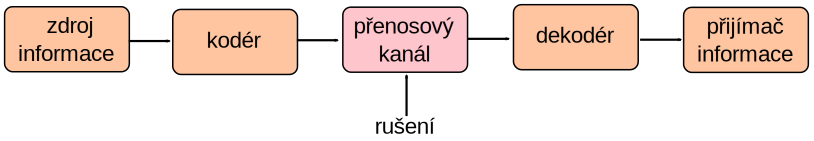
\includegraphics[width=0.9\linewidth]{tky_fig014.pdf}
        \caption{Nepřímý penos zprávy skrz přenosový kanál}
        \label{tky:fig014}
      \end{figure}

      Přenos signálu se může uskutečňovat v prvotní formě anebo v zprostředkované nepřímé formě, 
      kdy se pro přenos signálů používají pomocné tzv. \textbf{nosné signály}.
      
      Příkladem přenosu signálu v prvotní formě je přenos spojitých údajů o teplotě     
      prostřednictvím elektrického napětí ve vedení, přímo úměrné teplotě. 
      
      Při přenosu signálu v nepřímé formě se upravuje nosný signál tak, aby změny některého z jeho 
      parametrů zobrazovaly přenášenou zprávu. Tuto operaci vůči nosnému signálu nazýváme 
      \textbf{modulací}.
  % !TeX program = lualatex
% !TeX root = luaking.tex
% !TeX encoding = UTF-8
% !TeX spellcheck = cs_CZ
%---------------------------------------------------------------------------------------------------
% file tky1ch02.tex
%---------------------------------------------------------------------------------------------------
%======================= Kapitola: Signály a soustavy ==============================================
\setchaptertoc
\chapter{Signály a soustavy}\label{tky:IchII}
  \section{Úvod}\label{tky:IchIIsecI}
    \subsection{Příklady signálů}\label{tky:IchIIsecIssecI}
    \subsection{Definice signálů}\label{tky:IchIIsecIssecII}
    \subsection{Základní operace se signály}\label{tky:IchIIsecIssecIII}
    \subsection{Definice signálů}\label{tky:IchIIsecIssecIV}


% % !TeX spellcheck = cs_CZ
%============ Kapitola: Regulační technika =========================================================
\chapter{Regulační technika}\hypertarget{tky:regulace}
\minitoc
  \section{Kde se vzala, tu se vzala, zpětná vazba}


    \begin{wrapfigure}[15]{r}{0.5\linewidth} % \ref{tky:fig_feedback005}
      \centering
      \includegraphics[width=0.9\linewidth]{Reg_smycka03.png}
      \caption{Rychlost automobilu \cite[s.~9]{Roubal2011}.}
      \label{tky:fig_feedback005}
    \end{wrapfigure}
    Protože stojící automobil má aktuální rychlost menší než žádaných \SI{50}{\km\per\hour}, 
    sešlápneme pedál plynu a automobil začne zrychlovat, což pozorujeme na tachometru. V momentě, 
    kdy je aktuální rychlost větší než žádaná, uvolníme v souladu s radami od instruktora pedál 
    plynu a rychlost automobilu začne klesat, až bude opět menší než je žádaných 
    \SI{50}{\km\per\hour}. Takto budeme dokola sešlapávat a uvolňovat pedál plynu, až dosáhneme 
    žádané rychlosti. Jistě si umíme představit, že rychlost dosažení žádané rychlosti, závisí 
    nejen na vlastnostech samotného automobilu, ale také na našich řidičských dovednostech. V 
    případě opatrného řidiče, bude rozjezd pomalý a tak se rychlost bude blížit žádané pomalu. V 
    případě zbrklého řidiče, bude rozjezd velice razantní, což povede k rychlému překročení žádané 
    rychlosti. Následné neuvážené odlehčení plynového pedálu povede k prudkému poklesu rychlosti, 
    viz zelený průběh na obr. \ref{tky:fig_feedback005}. V obou případech se nelze hovořit o dobrém 
    stylu jízdy. V prvním případě se řidič rozjíždí příliš dlouho, na vozovce představuje překážku 
    a delší dobu zbytečně unikají splodiny do ovzduší. Ve druhém případě je motor při extrémních 
    otáčkách příliš hlučný, dochází k nekvalitnímu spalování a opět k úniku škodlivin do ovzduší. 
    Styl jízdy nepůsobí příliš uklidňujícím dojmem na ostatní řidiče a účastníky silničního provozu.
    
    Pro kvalitní dosažení žádané hodnoty rychlosti je třeba znát \emph{dynamický model} automobilu. 
    Tedy nejen sešlápni pedál plynu, uvolni pedál plynu, což můžeme považovat za \emph{statický 
    model} (v čase neproměnný), ale právě popis jak rychle se automobil rozjíždí, když takovým a 
    takovým způsobem sešlápneme pedál plynu. V regulační technice budeme mít dynamický model 
    systému tvořený převážně diferenciálními (pohybovými) rovnicemi. Modelováním reálných 
    dynamických systémů se budeme zabývat v kapitole \ref{TKY:sec002}. Procesu získávání modelu 
    fyzikální reality říkáme \textbf{identifikace systému} a v našem příkladě s automobilem ji 
    vlastně provádíme tím, že se učíme jezdit. Na identifikaci dynamických systémů a její praktické 
    aspekty se zaměříme v kapitole \ref{TKY:sec003}.

    V momentě, kdy máme dynamický model systému, přichází další krok a to je vlastní \textbf{návrh 
    regulátoru}, neboli návrh algoritmu řízení. V momentě, kdy už řidič ví, jak automobil reaguje 
    na změny vstupu, může dosáhnout žádané výstupní veličiny mnohem lépe, viz obr. 
    \ref{tky:fig_feedback003}. Na rozdíl od řidiče, jenž má naučený regulátor ve své hlavě, v 
    regulační technice budeme využívat různé matematické metody. Možná nás nyní napadne, že model 
    automobilu není pouze závislost mezi pedálem plynu a rychlostí automobilu. Chování automobilu 
    ovlivňuje samozřejmě mnoho dalších okolností, jako je přilnavost pneumatik k povrchu vozovky, 
    vlhkost vozovky a podobně. V momentě, kdy například zaprší, může řidič se svým regulátorem v 
    zatáčce opustit vozovku, pokud jsme příliš agresivní, protože se reálný systém změnil, ale jeho 
    model tuto informaci nemá. Opět tedy musíme vzít v potaz nové faktory a provést identifikaci 
    znovu, a tím získat více informací o chování systému za těchto podmínek. Pak bude řidič schopen 
    jezdit bezpečně za sucha i za mokra a tak dále. V regulační technice je vždy přesnost modelu 
    zásadní otázkou. Na jedné straně požadujeme model systému co nejpřesnější, abychom byli schopni 
    navrhnout dobrý regulátor. Na druhé straně se pro příliš složitý model navrhuje regulátor 
    obtížněji. Proto vždy musíme zvolit jistý kompromis tak, aby v modelu byly zahrnuty všechny 
    podstatné vlastnosti systému.

    Tím ale regulace nekončí. Například cena paliva není již dnes zanedbatelná, a tak budeme třeba 
    chtít jezdit s minimální spotřebou. To znamená, že musíme zjistit závislost spotřeby paliva na 
    stylu jízdy. Poté musíme definovat nějaké kritérium kvality regulace obsahující tuto závislost 
    a podle něho navrhnout nový regulátor, který zajistí minimální spotřebu paliva.  Problémů v 
    oblasti řízení je samozřejmě mnohem a mnohem víc  (odhadování a filtrace, robustní řízení a 
    nelineární systémy). My však zde tento příklad ukončíme s konstatováním, že v regulační 
    technice jde především o tyto body:
    \begin{itemize}\addtolength{\itemsep}{-0.5\baselineskip}
      \item určení vstupů a výstupů systému,
      \item identifikace systému (určení chování systému na výstupech pro nějaké chování vstupů),
      \item návrh regulátoru pro zajištění požadovaných vlastností; testování regulátoru na 
            počítači; aplikace regulátoru na reálném systému; případně návrh v nějakém smyslu 
            optimálního regulátoru.
    \end{itemize}
    
  \section{Regulační smyčka a základní typy PID regulátorů}\label{TKY:sec001}
    \begin{wrapfigure}[6]{r}{0.5\linewidth} % \ref{tky:fig_feedback003}
      \centering
      \includegraphics[width=0.9\linewidth]{Reg_smycka01.png}
      \caption{Regulační smyčka \cite[s.~215]{Roubal2011}.}
      \label{tky:fig_feedback003}
    \end{wrapfigure}
    Ve snaze řídit systémy rozeznáváme dva hlavní způsoby řízení:
      \begin{itemize}
        \item \textbf{přímovazební},
        \item \textbf{zpětnovazební}.
      \end{itemize}
    \textbf{Přímovazební řízení} (\emph{řízení v otevřené smyčce}), zvané také jako ovládání, má 
    jednodušší zapojení, ovšem jeho nevýhodou je nemožnost reagovat na poruchy či změny soustavy a 
    my se jím zde dále zabývat nebudeme. Naproti tomu \textbf{zpětnovazební řízení} (\emph{řízení v 
    uzavřené smyčce}), obecně označované jako \textbf{regulace}, porovnává \emph{výstup soustavy} 
    \(y(t)\) s \emph{požadovaným výstupem} \(w(t)\), a podle této informace generuje \emph{akční 
    zásah} \(u(t)\) do řízeného systému. Regulace nám tak dává mimo jiné možnost 
    \emph{stabilizovat} nestabilní soustavy.
    
    V této kapitole se budeme věnovat regulaci, regulační smyčce a základním typů regulátorů. 
    Ukážeme si dvě základní zapojení regulačních smyček a zavedeme jednotné názvosloví, zejména 
    proto, že toto názvosloví není ustálené. Vysvětlíme si některé míry kvality řízení a ukážeme 
    názorně na příkladech vlastnosti základních \textbf{PID regulátorů}. Zvláštní pozornost bude 
    věnována filtraci derivační složky u tohoto regulátoru. Konkrétní způsoby návrhu regulátorů si 
    ukážeme v následujících kapitolách.
    
  
  \section{Modelování fyzikálních systémů}\label{TKY:sec002}
    Doposud jsme se v předešlých kapitolách zabývali různými nástroji, jak popisovat dynamické 
    chování systémů. Šlo spíše o teorii rozdělenou do kapitol bez větších souvislostí. V této kar 
    kapitole bychom chtěli ukázat použití těchto teoretických poznatků na konkrétních příkladech 
    fyzikálních systémů. Odvodíme zde několik matematických modelů fyzikálních systémů a připravíme 
    k těmto modelům simulinkové soubory s virtuální realitou pro Matlab (The Mathworks, 2009).
    
  \section{Identifikace systémů}\label{TKY:sec003}
    
%---------------------------------------------------------------------------------------------------
\printbibliography[title={Seznam literatury}, heading=subbibliography]
\addcontentsline{toc}{section}{Seznam literatury}
% \input{../src/TKY/chap/Sensor_Temp.tex}
}{
  \LuaPartBckgrnd{titleBG_fractal1.png}
  \LuaPartTitle{TKY}{Technická kybernetika}{TKY}
  \parttoc
% DEBUG was off
%======================= Kapitola: Základy technické kybernetiky ===================================
  % !TeX spellcheck = cs_CZ
%{\tikzset{external/prefix={tikz/TKY/}}
% \tikzset{external/figure name/.add={ch01_}{}}
%======================= Kapitola: Základy technické kybernetiky ===================================
\setchaptertoc
\chapter{Základy technické kybernetiky}\label{tky:IchapI}
  \section{Vznik a vývoj kybernetiky}\label{tky:IchapIsecI}
    V časopise \casopisVesmir píše \textsc{Ivan M. Havel} na téma \uv{Kybernetika} následující: Před
    padesáti lety vznikla podivná věda: kybernetika. Na rozdíl od jiných věd si za předmět svého
    studia nezvolila nějaké věci, jako třeba šicí stroje nebo žáby, nýbrž určité vztahy, vlivy a
    jevy, které se v různých převlecích vyskytují na jinak zcela nepodobných místech. V rámci „čisté
    “ kybernetiky (na rozdíl od jejích aplikovaných verzí) jsou staronové pojmy – jako například
    zpětná vazba, řízení, regulace, automaty, sdělování, signál, informace, zpráva, komunikace,
    adaptace, stabilita, sebeorganizace, sebereprodukce – studovány především s důrazem na ty
    aspekty, které je osvobozují od konkrétních nositelů. Kybernetické zkoumání se tak vydalo napříč
    klasickými vědními obory – přesně v pojetí transdisciplinarity (\cite{Vesmir1998_11}).

    Kybernetické myšlení nebylo možná cizí ani myslitelům starověku. Mezi zlomky od
    \textsc{Hérakleita z Efesu} (cca 500 př. K.) najdeme například pozoruhodnou větu:
    \begin{center}
      \uv{Jedno je moudré: vědět, \\ že důmysl všechno řídí skrze vše.}
    \end{center}  

    \luagraphic[1]{tky_fig003.jpg}{\wikiNorbertWiener (\textasteriskcentered 26. listopadu 1894 -
      \textdagger 18. brezna 1964) byl americký matematik, který je považován za zakladatele
      kybernetiky. Kredit: monoskop.org}{tky:fig003}

    Nalákán slovem „řídí“ – \emph{kybernésai} – dovoluji si tuto větu s jistou interpretační
    smělostí číst jako oslavu kybernetiky. Každé řízení, nejen bicyklu, lodi nebo firmy, je ovládání
    či usměrňování něčeho (možná velkého, hmotného a odporujícího) bez vynaložení síly. Pravda,
    nějaká síla tu musí být, ta však je podstatně menší a zpravidla nezávislá na velikosti,
    hmotnosti a odporu toho, co je řízeno. Pak onen „důmysl“, který všechno řídí, má-li působit
    jinak než silou, musí být založen na informaci. S informací (v kvalitativním či sémantickém
    smyslu) je tu spojeno několikero činností: měření, pozorování či vnímání, rozpoznání toho, co je
    relevantní, rozhodnutí o tom, co se má dít, sdělení tohoto rozhodnutí tomu, co je řízeno,
    případně schopnost si z toho všeho brát ponaučení a tvořit operativní model světa i sebe sama.
    Pokud jde o ono řízení „všeho skrze vše“, lze nejspíš odkázat na vyznavače celistvosti, dle
    nichž je vše se vším propojeno rozsáhlou sítí vztahů, vazeb a kontextů (představte si jen
    přírodní ekosystém). Takto lze Hérakleitův zlomek převést do jazyka kybernetiky. A ten, jakkoli
    abstraktní, nabízí básnické metafory – třeba spojení řízení s důmyslem.


    Rozmanité definice kybernetiky mají jedno společné: nevymezují její hranice. Je to asi dobře –
    jinak by z ní byla jen další disciplína mezi ostatními, proti původnímu záměru. Takto je
    kybernetika tematicky otevřená a neměli bychom se zdráhat spojovat s ní rozličné novější
    myšlenky, nápady a směry bádání: od celulárních automatů, neuronových sítí, molekulárních a
    kvantových počítačů, kolektivních a kooperativních jevů, adaptivních, samoorganizujících a
    autopoietických systémů a genetických algoritmů až po inteligentní roboty, virtuální realitu a
    internetovou síť.
 
    Historicky poskytlo impuls ke vzniku novodobé kybernetiky řešení problému řízení palby
    protiletadlového dělostřelectva za 2. světové války. Na tomto úkolu pracoval také americký
    matematik \textsc{Norbert Wiener}. Výsledkem matematického i konstrukčního úsilí bylo, že mířič
    - člověk byl nahrazen přístrojem - zaměřovačem, který snímal údaje o současné poloze letadla, z
    ní vypočítával polohu v budoucích okamžicích a servomechanismem se přenášela informace od
    zaměřovače a počítače na kanóny. \textsc{Norbert Wiener} pak jako první zpracoval teorii
    automatizovaných systémů řízení pro účely protiletecké obrany. Tuto teorii zobecnil pro všechny
    druhy technických, biologických a společenských systémů. Shrnul ji ve své proslulé knize
    \emph{Kybernetika neboli řízení a sdělování v živých organismech a strojích} \cite{Wiener1961}.
    Tato kniha vyšla v roce \num{1948} a stala se světovým vědeckým bestsellerem. Svého autora
    proslavila jako zakladatele kybernetiky (\cite[s.~6]{Svarc1986}).

    \luagraphic[0.8]{tky_fig003b.jpg}{V roce 1948 vydal Wiener knihu s názvem \emph{Kybernetika aneb
      řízení a přenos informací v živém organismu a ve stroji}
      (\foreignlanguage{english}{Cybernetics: or Control and Communication in the Animal and the
      Machine, Paris: Hermann \& Cie, 1948}) v níž odhalil a formuloval zákonitosti při přenosu a
      zpracování informací. Objasnil podobnost v činnosti počítacích strojů a nervové soustavy. Jako
      zástupci Hermann Editions se M. Freymannovi podařilo najít kompromis a práva na knihu získal
      francouzský vydavatel. Poté, co spolu žili v Mexiku, byli Freymann a Wiener přátelé a byl to
      Freymann, kdo navrhl, aby Wiener napsal tuto knihu. V roce 1950 napsal populárnější výklad
      kybernetiky pro širší veřejnost pod názvem \emph{Kybernetika a společnost}. Kredit:
      monoskop.org}{tky:fig003b}
    
    Řešení praktických (a bohužel vojenských) problémů použití elektronických počítačů k řízení
    střel inspirovalo Wienera ke studiu řízení se zpětnou vazbou. Spolu s neurofyziologem
    \textsc{Arturem Rosenbluethem} hledali analogie k technickým zpětnovazebním systémům pro
    navádění střel na pohyblivý cíl. Takovou analogii nalezli u některých biologických systémů -
    konkrétně v nervové soustavě živých organismů. Myšlenka zpětné vazby u živých a neživých systémů
    se stala základem kybernetické koncepce vyložené v citované knize. Hledání analogií mezi živým
    organismem a strojem (případně také společnosti) znamená postihnout společné znaky zdánlivě
    naprosto různorodých systémů. A tyto analogie pak vedou k používáni matematického a logického
    aparátu i tam, kde to dosud nebylo možné.
    
    Nemůžeme ovšem nevidět všechny předcházející tendence a faktory v historii společnosti, které
    vedly ke vzniku kybernetiky. Bylo by nesprávné tvrdit, že pouze \textsc{Norbert Wiener} a
    několik jeho spolupracovníků vytvořilo kybernetiku. Její vznik byl pokračováním určité tendence,
    která se projevovala již dávno předtím. Kybernetiku musíme chápat jako výsledek rozvoje
    materiálních sil lidské společnosti a rozvoje vědeckého poznáváni světa.
    
    Kybernetika jako taková vznikla na základě celé řady interdisciplinárních setkání významných
    poválečných intelektuálů v průběhu let 1944 – 1953, mezi které patřili \textsc{Wiener},
    \textsc{John von Neumann}, \textsc{Warren McCulloh}, \textsc{Claudie Shannon}, \textsc{Heinz von
    Foerster}, \textsc{W. Ross Ashby} \cite{Ashby1956}, \textsc{Gregory Bateson} a \textsc{Margaret
    Mead}. Pod záštitou nadace \textsc{Josiaha Macyho Jr.} vešla tato setkání ve známost jako Macyho
    konference o kybernetice. Z původního zaměření na stroje a zvířata se zájem kybernetiky rychle
    rozšiřuje na oblasti vědomí (\textsc{Bateson} a \textsc{Ashby}) a sociálních systémů (tj.
    Stafford Beerova kybernetika managementu), čímž se vrací k původnímu Platonovu pojetí
    kybernetiky jakožto vědy o kontrole vztahů ve společnosti. 
    
    Samotný název kybernetika \foreignlanguage{greek}{κυβερνητικός} pochází z řeckého slova
    \uv{kybernétés} neboli \uv{kormidelník}, \uv{člověk řídící loď\,}. Objevuje se v dílech řeckých
    filosofů, např. v Platonově díle Dialogy\footnote{Platónova díla mají vesměs formu dialogu
    (rozhovoru), kde většinou vystupuje Sókratés jako hlavní postava.}; zde se tímto termínem
    vyjadřuje \uv{umění řídit lodě a administrativně spravovat provincie}. V novověku použil termín
    kybernetika \textsc{A. M. Ampére} v encyklopedii a to ve smyslu \uv{vědy o řízení společnosti}.
    Termín se neujal a tak to byl až Wiener, který jím nazval nově vznikající vědní obor.
    (\cite[s.~6]{Svarc1986}).

    \subsection{Základní pojmy kybernetiky a její vymezení}
      Pro kybernetiku jsou charakteristická tři základní hlediska \ref{tky:fig004}, z kterých nazírá
      na problémy a z kterých dané problémy řeší.

      \luagraphic[0.8]{tky_fig004a.pdf}{Základní hlediska kybernetiky
        (\cite[s.~7]{Svarc1986})}{tky:fig004}
      
      Tím se dostáváme k nejzákladnějších pojmů kybernetiky: \textbf{systém}, \textbf{informace} a
      \textbf{řízení}, Z těchto hledisek se pak vyvinuly základní obory teoretické kybernetiky -
      teorie systémů, teorie informace a \hyperlink{tky:regulace}{teorie řízení} (kapitola \ref{}).
      
      Jako příklad vysvětlující tato hlediska kybernetiky si zvolme automobil. Automobil je z 
      hlediska konstruktéra složité technické zařízení, sloužící k dopravě osob a nákladu, které je 
      vyrobeno z různých materiálů. Je sestaven z mnoha součásti, pohon je motorem spalovacím nebo 
      vznětovým, k provozu jsou nezbytné látky jako benzín, oleje, voda, ... .To vše je důležité a 
      podstatné z hlediska konstruktéra automobilu, ale ne z hlediska kybernetiky.

      \luagraphic[1]{tky_fig017.pdf}{Automobil}{tky:fig017}

      Jaká jsou tedy hlediska kybernetiky? Kybernetika vidí v automobilu především tzv.
      \textbf{dynamický systém}, jehož činnost je spojena s člověkem - řidičem a je ve vztahu k
      okolnímu světu (\ref{tky:fig017}). Automobil uvažovaný jako systém se skládá ze dvou
      podsystémů (subsystémů). Prvním z nich je vlastní vozidlo, druhým je člověk
      (\ref{tky:fig001}). Každý podsystém se pak skládá z elementárních jednotek, vzájemně
      propojených, tzv. \emph{prvků systému}. Mezi prvky systému existují různé vztahy. Ale nejenom
      mezi prvky nebo podsystémy existuji vztahy.

      Automobil není izolovaným systémem a proto má také četné vztahy k okolí. K okolí \uv{systému 
      automobil} patří ty části okolního světa, které mají vliv na jeho činnost. Jsou to např. 
      vozovka, křižovatky, zatáčky, jiná vozidla, chodci, dopravní značky apod. Na všechny vlivy 
      okolí reaguje systém automobil určitým způsobem. Reakce systému na okolí se nazývá 
      \textbf{chování systému}. 

      \luagraphic[0.8]{tky_fig001.pdf}{Automobil jako dynamický systém
        (\cite[s.~7]{Svarc1986})}{tky:fig001}
      
      Pokud sleduje kybernetika automobil tímto způsobem, jedná se o \emph{systémové hledisko}
      kybernetiky  (obr. \ref{tky:fig001}). Předběžně si vymezme pojem systém jako soubor prvků,
      mezi nimiž existuji nějaké funkční vztahy. 
      
      Sledujeme-li vzájemné působeni systému a jeho okolí, jde o druhé základní kybernetické
      hledisko. Poněvadž se toto působení realizuje výměnou informací mezi systémem a okolím,
      mluvíme o \emph{informačním hledisku}. Pod pojmem informace si představíme zprávu, která má
      pro některé ze zúčastněných systémů určitý význam. Nositelem informace jsou tzv.
      \textbf{signály}.
      
      Doposud jsme uvažovali prostou výměnu informací mezi dvěma systémy. Je-li ale informace 
      využívána přijímacím systémem pro další činnost, pro dosažení určitého předem stanoveného 
      cíle, pak už se jedná o \emph{řízení}. Pojem řízení vymezíme jako \emph{proces výměny 
      informace mezi dvěma systémy}, který se uskutečňuje plánovitě pro dosažení určitého cíle. Při 
      řízení se uplatňuje informační působení řídicího systému na řízený systém. Tím se dostáváme k 
      třetímu kybernetickému hledisku a to je \emph{hledisko řízení}. Zdůrazněme, že toto hledisko 
      provádí pouze informační bilancování a nikoliv látkové nebo energetické.
      
      Vraťme se k našemu automobilu. Systém automobil má dva podsystémy vozidlo a řidiče. Mezi nimi 
      probíhá informační výměna, jejíž cílem je pohyb automobilu po stanovené dráze, např. v přímém 
      směru. Řidič reaguje na nerovnosti vozovky nebo na boční vítr, které vychyluje vozidlo z 
      přímého směru tím, že pootáčí volantem. Řidič je tedy řídícím systémem a vozidlo řízeným 
      systémem a výměna informací probíhá za účelem udržení pohybu vozidla v přímém směru - jedná 
      se o \textbf{proces řízení}.
      
      Všimněme si momentu, že řidič otáčí volantem na základě toho, jaký účinek vyvolalo předchozí 
      pootočení. Neustále sleduje směr vozidla a vyrovnává odchylky od přímého daného směru. Takový 
      způsob řízení označujeme v kybernetice jako \textbf{řízení se zpětnou vazbou} neboli 
      \textbf{regulace}. Systémy se zpětnou vazbou se tedy nazývají \textbf{regulační systémy}. 
      Systém automobil (řidič + vozidlo) můžeme pokládat za regulační systém, který je regulován na 
      přímý směr jízdy.
      
      Poněvadž systémy řízení se zpětnou vazbou, tedy regulační systémy, jsou pro kybernetiku 
      charakteristické, nazýváme třetí kybernetické hledisko také \emph{hlediskem regulačním}. 
      Samozřejmě existuje rovněž \textbf{řízení bez zpětné vazby}; v tom případě se mluví jen o 
      \textbf{systémech řízení} nebo o \textbf{systémech ovládání}.
      
      Řízení jako vzájemná interakce mezi systémy nebo mezi systémem a okolím probíhá vždy v 
      určitém pořadí činnosti některého ze systémů. obvykle řídicího. Soubor pravidel, podle něhož 
      řídící systém vykonává sled činností za účelem řízení, se nazývá \textbf{algoritmus}. Obecně 
      je \emph{algoritmus soubor pravidel, podle něhož probíhá řízení}.
      
      U zvoleného příkladu s automobilem bychom mohli například sestavit algoritmus spouštění 
      motoru, algoritmus vyjíždění automobilu, algoritmus předjíždění, atd. Algoritmy jsou objektem 
      zkoumání jednoho z oborů teoretické kybernetiky - \emph{teorie algoritmů}.
      
      Po předběžném objasnění základních hledisek kybernetiky a základních pojmů kybernetiky je 
      možné se pokusit vyložit, ce vlastně kybernetika je a čím se zabývá. Jednotlivý autoři, kteří 
      se pokoušejí podat definici kybernetiky, protěžují více nebo méně některé ze tří základních 
      kybernetických hledisek (hledisko systémové, hledisko informační, hledisko řízení). Většina 
      starších definic kybernetiky vychází z klasické definice jejího uznávaného zakladatele 
      Norberta Wienera, který ji definoval jako \uv{vědu o řízení a sdělování v živých organismech 
      a strojích}. Tato definice, která je nerozlučně spjata s jejím vznikem, protěžuje hledisko 
      informační a hledisko řízení. Jejím nedostatkem je, že ještě nedoceňuje systémový přístup, 
      systémové hledisko při řešení problémů. Dále jako objekty zkoumání (tedy systémy) zahrnuje 
      pouze živé organismy a stroje. Nezahrnuje tedy další důležité objekty zkoumané dnešní 
      kybernetikou jako jsou objekty společenské a ekonomické a neuvažuje systémy matematické, 
      lingvistické a další a z technických systémů dnes tak různorodých se omezuje jen na stroje. 
      Ani informační hledisko této definice není úplné, protože se omezuje pouze na přenos 
      informací a neuvažuje dnes tak důležité procesy uchování a zpracováni informace.
      
      Podobnými nedostatky se vyznačovaly definice kybernetiky dalších autorů. Byl to vždy 
      jednostranný přístup a neúplnost jednotlivých hledisek. Proto nelze žádnou z definic 
      akceptovat s definitivní platností.
      
      Nebudeme se tedy snažit za každou cenu zformulovat vyčerpávající definici, ale uveďme si 
      charakteristické rysy kybernetiky jako vědy.
      
      Kybernetika se zabývá různými rozdílnými problémy, které však byly většinou známy a zkoumány 
      před vznikem kybernetiky, např. krevní oběh, podmíněný reflex, radiolokace, konstrukce 
      počítačů, řízení různých technických zařízení, kódování atd. Kybernetika vnáší do těchto 
      problémů nový pohled, neboť si všímá toho, že na určitém stupni organizace a vývoje systémů 
      vzniká nový proces řízení. Tento proces se projevuje výměnou informací v systémech, kterým se 
      chování systémů zaměřuje k určitému cíli.
      
    \subsection{Rozdělení kybernetiky}
      Z praktického hlediska můžeme kybernetiku rozdělit podle přístupu a aplikací:
      
    \begin{description}[leftmargin=3em,labelindent=1em, style=nextline]
      \item[Teoretická kybernetika] studuje především obecné vlastnosti a chování systémů. Zabývá 
            se obecným popisem vlastností a chování systémů. Z tohoto pohledu zahrnuje teoretická 
            kybernetika \emph{teorii systémů} a \emph{teoretickou informatiku}.
      
      \item[Aplikovaná kybernetika] představuje použití kybernetického přístupu při analýze, 
      modelování a simulaci a návrhu systémů, dále aplikuje poznatky kybernetiky do dalších 
      oblastí. Aplikovaná kybernetika zasahuje do mnohých oblastí lidské činnosti - zahrnuje totiž 
      mj. následující obory:
    \end{description}
 
  \section{Teorie systémů}\label{tky:IchapIsecII}
     Teorie systémů je jedna ze základních disciplin teoretické kybernetiky. Na druhé straně je ale 
     teorie systémů součásti tzv. \emph{obecné teorie systémů}, jejíž principy rozpracoval americký 
     biolog Ludwig von Bertalanffy. Pokusme se o vymezení vztahu mezi kybernetikou a teorií systémů.
     \cite[s.~11]{Svarc1986}.
     
     Obecná teorie systémů studuje systémy libovolné povahy, přičemž se zajímá o charakter prvků 
     systému, charakter vazeb mezi prvky a chování systému. Důležitým pojmem je zde \textbf{vazba 
     mezi prvky} a pojem \textbf{chování systémů}. Zatímco obecná teorie systémů se zajímá o 
     libovolný druh vazeb mezi prvky a libovolné chování systémů, kybernetiku zajímá specifický 
     druh vazeb a specifické chování. Kybernetika studuje pouze ty vazby, které jsou realizovány 
     přenosem informace a chování, které lze zahrnout pod \textbf{pojmem řízení}. A to je náplní 
     teorie systémů jako disciplíny teoretické kybernetiky.
     
     \textbf{Přenos informace} a \textbf{řízení} nejsou od sebe \emph{oddělitelné}. Aspoň tak, že 
     není možné řízení bez přenosu informace. Je však už sporné, je-li každý přenos informace již 
     řízením. Můžeme říci, že systémy mezi nimiž probíhá proces řízení musí mít určitou specifickou 
     strukturu a musí být mezi nimi zajištěn přenos informace. Pokud existuje pouhá výměna 
     informací mezi systémy, mluvíme o \textbf{informačních systémech}.
     
     \emph{Obecnou teorii systémů} tedy \emph{nemůžeme} zahrnout do kybernetiky; s kybernetikou má 
     společnou jen určitou část, která je zaměřena na studium systémů z hlediska informačních 
     vazeb. Hlavním úkolem obecné teorie systémů je postihnout a vyjádřit exaktním způsobem 
     vlastnosti a vztahy ve složité a dynamické (v čase se měnící) \emph{objektivní realitě} tak, 
     aby se neztratila její komplikovaná struktura a složitost. Jestliže dříve byl nějaký přírodní 
     nebo společenský jev pokládán za vysvětlený, když se nalezla jeho příčina, pak při systémovém 
     přístupu musí bý nalezena struktura a dynamika každého objektu, který se na daném jevu podílí.
     
     \subsection{Charakteristika základních pojmů z teorie systémů}
       Pro práci se složitými a rozsáhlými objekty, jako jsou například řízení výrobních a
       technologických procesů, je nutný \textbf{systémový přístup}. Například technologický proces
       exploatace uhlí na hlubinných nebo povrchových dolech, je charakterizován různorodostí
       pracovních činností, na něž působí celá řada vlivů. Komplexně jde o mnoha rozměrný
       dynamický celek, který se neustále mění v čase a v prostoru.
       
       \emph{Systémový přístup spočívá v tom, že jevy vyskytující se při řešení vzniklých problémů, 
       jsou chápany komplexně, se všemi souvislostmi ve svém dynamickém vývoji.}
       
       V souvislosti se systémovým přístupem je nejdůležitějším pojmem \textbf{systém}. Jestliže 
       chceme v dalším uvést základní pojmy teorie systémů, musíme nejdříve tento pojem vysvětlit. 
       Předběžně jsme ho vymezili jako \emph{soubor prvků, mezi nimiž existuji nějaké funkční 
       vztahy a který má jako celek vztah ke svému okolí}. Jinými slovy: \emph{Stanovíme- li 
       vztahy, mezi na sebe navzájem působících objektů materiální, ale i nemateriální povahy, je na
       objektivní realitě vytvořen systém.} Jiní autoři podávají tyto definice:
       \begin{itemize}[noitemsep]
         \item Bertalanffy (1956): Systém je komplex prvků nacházejících se ve vzájemné interakci.
         \item Hall - Fagen (1966): Systém je souhrn prvků spolu se vztahy mezi prvky a mezi jejich 
               vlastnostmi.
       \end{itemize}

       \begin{definition}
        \textbf{Systém} je definován jako účelově uspořádaná množina prvků a množina vazeb mezi 
        nimi, s dynamickým chováním, které společně určují vlastnosti celku.
        \begin{equation}
          \mathscr{S} = \{S,R \},
        \end{equation}
        kde
        \begin{description}[leftmargin=5em,style=nextline]
          \item[\hspace{2em}\(S \ldots\)] \emph{množina všech prvků},
          \item[\hspace{2em}\(R \ldots\)] \emph{množina relací mezi prvky, reprezentující vzájmené 
                                         funkční vztahy jednotlivých prvků a vztah systému k okolí.}
        \end{description}
       \end{definition}
       
       V rámci dekompozice systému lze vyčlenit \textbf{podsystém}. Podsystém je podmnožina
       systémových prvků a vazeb, která je z nějakého důvodu vyčleněna ze systému a je chápána
       jako nový systém nebo jako prvek.
       
      \begin{definition}
        \textbf{Prvek} je část systému, který tvoří na dané rozlišovací úrovni dále nedělitelný
        celek, jehož strukturu nechceme, nebo již nemůžeme v rámci analýzy rozlišit.
      \end{definition}
       
       \begin{tcnote}
         \textbf{Rozlišovací úrovní} se označuje stupeň podrobnosti zkoumání systému. Změnou        
         rozlišovací úrovně se může dřívější prvek systému stát podsystémem, popřípadě i systémem a 
         naopak. Dekompozicí systému na jednodušší prvky, se zvyšuje rozlišovací úroveň.
       \end{tcnote}
       
     \subsection{Klasifikace systémů}
       Někdy rozlišujeme pojem \textbf{statický} a \textbf{dynamický systém}, ale spíš známe pouze 
       systémy dynamické. Statický systém je totiž v čase konstantní, neměnný. Mezi statické 
       systémy můžeme někdy zařadit i systémy, u nichž se vlastnosti prvků mění velmi pomalu. V 
       přírodě se statické systémy prakticky nevyskytují, spíše se jedná o systémy s pomalou změnou 
       vlastností na čase. Naproti tomu dynamický systém je takový systém, u kterého existuje 
       alespoň jedna proměnná závislá na čase. Většina systémů je dynamických. V dalším textu jsou 
       proto popsány především \textbf{dynamické systémy a řídicí (regulační) systémy se zpětnou 
       vazbou}.
       
       Dynamické vlastnosti lineárních systémů lze popsat lineárními diferenciálními rovnicemi s 
       konstantními koeficienty a operátorovými přenosy. Dynamické vlastnosti nelineárních systémů 
       lze popsat nelineárními diferenciálními rovnicemi.
       
       Existují dvě možnosti studia dynamického systému. Prvním způsobem je zkoumání \emph{vnitřní 
       struktury systému}, tzn. vnitřní závislosti prvků a dále nás zajímají, jaké vnitřní změny 
       vznikají v systému při působení vnějších vlivů. To je podstatou \textbf{vnitřního popisu 
       dynamického systému}.
       
       Druhým způsobem je pojímání systému jako celek a studování pouze otázky, jaké výsledné 
       reakce systému vyvolávají vnější vlivy. Tomuto druhému způsobu se budeme věnovat při 
       \textbf{vnějším popisu dynamických systémů}.
     
     
  \section{Teorie informace}
    \textbf{Informace} jako stěžejní pojem kybernetiky, je pojem značně široký a hodně diskutovaný. 
    Je používán v celé řadě definic vymezujících předmět kybernetiky jako vědy, přičemž informační 
    hledisko považují někteří autoři za nejdůležitější.
      
    Přesná definice pojmu informace neexistuje. Obecně se tento pojem používá volně, v intuitivním 
    chápaní se vztahuje k pojmům jako zpráva, údaj, poznatek apod. Z hlediska kybernetiky je toto 
    chápáni příliš zúženo, neboť kybernetika sleduje přenos informace mezi dvěma nebo více systémy 
    s tím, že cílem přenosu může být řízení chování některého ze systému. Kybernetika říká, že 
    informace je jakékoliv sdělení, kterého lze reálně (právě nyní) nebe potenciálně (v budoucnu 
    při vhodné příležitosti) použit k řízení systému.
    
    Pojem informace je \emph{pojmem abstraktním} a jako takový má \emph{nehmotnou povahy}. 
    Současně však informace má smysl jen ve spojení s hmotou a to jak z hlediska přenosu, tak z 
    hlediska obsahu (i abstraktní představy jsou spjaty s existenci hmoty).
    
    Informace (sděleni) má
    \begin{itemize}\addtolength{\itemsep}{-0.4\baselineskip}
      \item \textbf{formu},
      \item \textbf{obsah},
      \item \textbf{význam}.
    \end{itemize}
    \textbf{Forma} informace neboli sdělení musí být přístupná systémům, mezi nimiž dochází k 
    výměně informaci a je důležitá pro proces přenosu informace. Pro proces řízení systémů je 
    podstatný \textbf{obsah a význam informace} (sdělení). \textbf{Sdělení} je \emph{informační, 
    sémantický a pragmatický obsah}. \textbf{Informační obsah} vyjadřuje kvantitativní míru 
    informace v dále definované jednotce \textbf{bit}. Používáme pro něj termín míra či množství 
    informace. \textbf{Sémantický obsah} vyjadřuje významovou stránku znaků při jazykové komunikaci 
    a nedá se měřit (\emph{sémantika} - nauka o významu slov). \textbf{Pragmatický obsah} určuje 
    významnost sdělení a prioritu jednotlivých zpráv pro příjemce.
    
    Každá forma hmoty, která nese informaci se nazývá \textbf{zpráva}. Zpráva je hmotným nositelem 
    informace. Zpráva je způsob vyjádření informace textem, obrazem, řečí, posloupností znaků atd. 
    Zpráva může být tedy např. číslo (posloupnost číslic), abecední text (posloupnost písmen), 
    spouštěcí signál (posloupnost napěťových úrovní). Pojmy informace a zpráva nelze zaměňovat. 
    Informace jo pojem abstraktní, zpráva jo konkrétní materiální formou informace, bez níž by 
    informace neměla smysl a nemohla by být přenášena a působit na systémy, kterým je určena. Pojem 
    zpráva bývá někdy nahrazován užším pojmem \textbf{signál}. Signál je fyzikální realizace zprávy 
    ve formě elektrického proudu resp. elektromagnetických vln.
      
    Sledujeme-li blíže jakoukoliv dostatečně dlouhou zprávu, pak zjistíme, že je vždy vytvářena z 
    posloupnosti nějakých základních elementů - \textbf{prvků}. Možný počet odlišných prvků, ze 
    kterých je taková zpráva vytvářena, může být bud \emph{konečný} nebo \emph{nekonečný}. Tak 
    např. psaná zpráva ve formě českého textu je posloupností různých kombinací písmen české 
    abecedy. Možný počet různých písmen - prvků je konečný a je dán počtem písmen české abecedy.
      
    Základní prvky, ze kterých je vytvářena zpráva, bývají obecně nazývány \textbf{písmena} a celý 
    \emph{soubor} všech \emph{možných prvků} bývá nazýván \textbf{abecedou zdroje}. Zpráva je pak 
    vytvářena výběrem prvků z abecedy zdroje a jejich sestavou v posloupnost prvků. Přitom 
    libovolný prvek abecedy se může ve zprávě libovolně opakovat. Abychom mohli odlišovat prvky 
    abecedy od prvků, z nichž je sestavena konkrétní realizace zprávy, budeme libovolný prvek 
    realizace zprávy nazývat \textbf{symbol}. Nechť má abeceda zdroje celkem \(s\) možných různých 
    prvků. Nechť je délka zprávy, tj. počet symbolů, z nichž je složena realizace zprávy, dána 
    počtem \(L\) symbolů. Celkový možný počet \(L\) různých realizaci zpráv délky \(n\), které 
    mohou být produkovány zdrojem s abecedou o \(s\) prvcích a které se budou lišit nejméně v 
    jednom symbolu, je
    \begin{equation}\label{tky:eq0001}
      L = s^n
    \end{equation}
    (počet všech možných \emph{variací n symbolů s opakováním}, které lze vytvořit z \(s\) prvků).
    
    Má-li abeceda zdroje \emph{konečný počet} \(s\) možných prvků, pak takový zdroj nazýváme 
    zdrojem \textbf{diskrétních zpráv} (diskrétní zdroj). Má-li abeceda zdroje \emph{nekonečný 
    počet prvků}, pak ho nazýváme zdrojem \textbf{spojitých zpráv} (spojitý zdroj).
    
    \begin{example}
      Kolik zpráv o délce \num{10} symbolů můžeme vytvořit z abecedy o \num{2} písmenech?
      \newline
      Řešení: Počet realizaci \(L\) zpráv je dán vztahem (\ref{tky:eq0001})
      \begin{equation*}
        L = s^n = 2^{10} = 1024
      \end{equation*}      
    \end{example}
      
    \subsection{Přenos zpráv}
      Zprávu lze přenést buď \emph{přímo}, přenesením nosného média (pergamen, magnetická páska, 
      optický disk), anebo \emph{nepřímým} způsobem prostřednictvím \emph{signálu}, který je 
      realizací zprávy ve formě změn některé fyzikální veličiny, nejčastěji elektrického proudu.
      
      Při nepřímém způsobu \textbf{zdroj informace} generuje prostřednictvím \textbf{kodéru} 
      (kódovacího zařízeni) signály, které se přenáší \textbf{kanálem}. Kanál je vlastně cesta, 
      která přenáší změny dané fyzikální veličiny, aby mohla být zpráva přenesena z jednoho místa 
      na druhé. Je tvořený prostředím, kterým se přenáší signál. Může to být např. telefonní 
      vedeni, trubka pro přenos tlakového signálu, akustické nebe elektromagnetické vlnění.
      
      Na výstupu kanálu je signál přijímán \textbf{příjemcem informace} (Člověk nebe zařízeni). 
      Zná-li příjemce zákon, podle kterého byla provedena transformace zprávy na vstupu kanálu, pak 
      může určit zprávu obsaženou v přijatém signálu. To provede tzv. \emph{dekódováním} v zařízeni 
      zvaném \textbf{dekodér}. Souhrn všech uvedených objektů vytváří \textbf{sdělovací soustavu}.

      \begin{figure}[ht!]
        \centering
        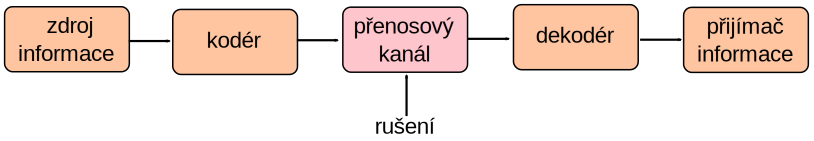
\includegraphics[width=0.9\linewidth]{tky_fig014.pdf}
        \caption{Nepřímý penos zprávy skrz přenosový kanál}
        \label{tky:fig014}
      \end{figure}

      Přenos signálu se může uskutečňovat v prvotní formě anebo v zprostředkované nepřímé formě, 
      kdy se pro přenos signálů používají pomocné tzv. \textbf{nosné signály}.
      
      Příkladem přenosu signálu v prvotní formě je přenos spojitých údajů o teplotě     
      prostřednictvím elektrického napětí ve vedení, přímo úměrné teplotě. 
      
      Při přenosu signálu v nepřímé formě se upravuje nosný signál tak, aby změny některého z jeho 
      parametrů zobrazovaly přenášenou zprávu. Tuto operaci vůči nosnému signálu nazýváme 
      \textbf{modulací}.
%======================= Kapitola: LTI systém ======================================================
  % !TeX program = lualatex
% !TeX root = luaking.tex
% !TeX encoding = UTF-8
% !TeX spellcheck = cs_CZ
%---------------------------------------------------------------------------------------------------
% file tky1ch02.tex
%---------------------------------------------------------------------------------------------------
%======================= Kapitola: Signály a soustavy ==============================================
\setchaptertoc
\chapter{Signály a soustavy}\label{tky:IchII}
  \section{Úvod}\label{tky:IchIIsecI}
    \subsection{Příklady signálů}\label{tky:IchIIsecIssecI}
    \subsection{Definice signálů}\label{tky:IchIIsecIssecII}
    \subsection{Základní operace se signály}\label{tky:IchIIsecIssecIII}
    \subsection{Definice signálů}\label{tky:IchIIsecIssecIV}


%========================= Kapitola: Regulační technika ============================================
  \input{../src/TKY/chap/tky1ch03.tex}
%========================= Kapitola: Senzory a akční členy =========================================
  % !TeX program = lualatex
% !TeX root = luaking.tex
% !TeX encoding = UTF-8
% !TeX spellcheck = cs_CZ
%---------------------------------------------------------------------------------------------------
% file tky1ch10.tex
%---------------------------------------------------------------------------------------------------
%===============Kapitola:Senzory a akční členy =====================================================
\setchaptertoc
\chapter{Senzory a akční členy}
  \section{Snímače tepelných veličin}
    \href{http://cs.wikipedia.org/wiki/Teplota}{Teplota} je charakteristika tepelného stavu hmoty.
    V obecném významu je to vlastnost předmětů a okolí, kterou je člověk schopen vnímat a přiřadit
    jí pocity studeného, teplého či horkého. V přírodních a technických vědách a jejich aplikacích
    je to \emph{skalární intenzivní veličina}, která je vzhledem ke svému pravděpodobnostnímu
    charakteru vhodná k popisu stavu ustálených makroskopických systémů. Teplota souvisí s
    kinetickou energií částic látky.

    Teplota je základní fyzikální veličinou soustavy \texttt{SI} s jednotkou kelvin (\si{\kelvin}) a
    vedlejší jednotkou stupeň Celsia (\si{\degreeCelsius}). Nejnižší možnou teplotou je teplota
    absolutní nuly (\SI{0}{\kelvin}, resp. \SI{-273.15}{\degreeCelsius}), ke které se lze libovolně
    přiblížit, avšak nelze jí dosáhnout.
         
    Do této skupiny patří především rozsáhlá část snímačů teploty. Z hlediska měřených veličin
    můžeme provést následující rozdělení.
    \begin{enumerate}[noitemsep]
      \item \textbf{Snímače teploty}
        \begin{enumerate}[label=\emph{\alph*}),noitemsep]
          \item emph{Snímače pro dotykové měření} 
            \begin{itemize}
              \item elektrické
               \begin{itemize}
                 \item odporové kovové
                 \item odporové polovodičové
                 \item termoelektrické
                 \item polovodičové 
               \end{itemize}   
              \item dilatační
              \item termoelektrické
              \item tlakové
              \item speciální
            \end{itemize}
          \item \emph{Snímače pro bezdotykové měření}
            \begin{itemize}
              \item monochromatické pyrometry
              \item pásmové pyrometry
              \item radiační pyrometry
            \end{itemize}
        \end{enumerate}
      \item \textbf{Snímače tepla}
      \item \textbf{Snímače tepelného toku}
    \end{enumerate}  
       
    \subsection{Elektrické teploměry}
      \subsubsection{Odporové snímače}
        Odporové snímače využívají princip změny elektrického opdoru vlivem změny teplot. Základním
        požadavkem kladeným na materiál snímače je co největší a stálý teplontí součinitel odporu a
        zároveň co největší měrný odpor. Pro tyto účely se používají kovové a polovodičové
        materiály.
        
      \subsubsection{Kovové odporové snímače} 
        Jsou to především čisté kovy, které se používají pro realizaci vlastního odporového
        článku. Požadavkem je, aby nereagovaly s izolačním nebo ochranným krytem. Jakékoliv
        chemické nebo fyzikální vlivy by mohly způsobit nestálost odporu při stálé teplotě,
        Použitý materiál nemá vykazovat změnu teplotního součinitele odporu s časem (stárnutí) a
        hysterezi. Nejčastěji používanými materiály je \emph{platina, nikl, měď, slitina
        stříbro-zlato} a další \cite[s.~96]{Zehnula1983}.
          
        Platina je výhodná pro velkou chemickou stálost, vysokou teplotou tavení a možností
        dosažení vysoké čistoty. Pro snímače teploty se používá tzv. fyzikálně  čistá platina,
        jejíž čistota se pohybuje kolem 99,93 až 99,99 \% Pt. Měření ukázala, že změny
        základního odporu u sériově vyráběných přesných teploměru se pohybují kolem
        \num{5e-6} \(R_o\) (což odpovídá \SI{0.001}{\kelvin}), u nejlepších teploměrů je tato
        hodnota ještě o řád menší. Proto se používá platina pro etalonový teplměr v oblasti
        teplot \SI{-259.34}{\degreeCelsius} až \SI{630.74}{\degreeCelsius}.
        
        Závislost odporu na teplotě pro rozsah \num{0} až \SI{630}{\degreeCelsius} se vyjadřuje
        rovnicí
        \begin{equation}\label{SAC:kov_Ro1}
          R_\vartheta = R_0(1 + A\vartheta + B\vartheta^2)
        \end{equation}
        kde 
        \begin{description}[leftmargin=5em,labelindent=2em, style=nextline]
          \item[\(R_0\)]        \(\ldots\) \emph{odpor při \SI{0}{\degreeCelsius}}, 
          \item[\(\vartheta\)]  \(\ldots\) \emph{teplota ve \si{\degreeCelsius}}, 
          \item[\(A\)]          \(\ldots\) \emph{konst (\SI{3.9075e-3}{\per\degreeCelsius})},
          \item[\(B\)]          \(\ldots\) \emph{konst (\SI{-0.575e-6}{\per\degreeCelsius})}. 
        \end{description}

        V rozmezí od \SI{0}{\degreeCelsius} do \SI{-190}{\degreeCelsius} se vyjadřuje
        závislost odporu na teplotě rovnicí
        \begin{equation}\label{SAC:kov_Ro2}
          R_\vartheta = R_0[1 + A\vartheta + B\vartheta^2 + C(\vartheta - 100)\vartheta^3)]
        \end{equation}       
%=============== Seznam literatury ================================================================= 
  \printbibliography[title={Seznam literatury}, heading=bibliography]
}
    %===================================================================================================
% Teorie elektrických obvodů
% TEO.tex
%===================================================================================================
% notes:
%~~~~~~~~~
% \ref{teo:eq148}
% \ref{teo:fig021}
% \ref{fyz:exam001}
% \ref{fyz:tab000}
%---------------------------------------------------------------------------------------------------
% Setting path to image 
\graphicspath{{../src/TEO/img/}}
%---------------------------------------------------------------------------------------------------
%                            /$$$$$$$$ /$$$$$$$$  /$$$$$$ 
%                            |__ $$__/| $$_____/ /$$__  $$
%                              | $$   | $$      | $$  \ $$
%                              | $$   | $$$$$   | $$  | $$
%                              | $$   | $$__/   | $$  | $$
%                              | $$   | $$      | $$  | $$
%                              | $$   | $$$$$$$$|  $$$$$$/
%                              |__/   |________/ \______/ 
%---------------------------------------------------------------------------------------------------
\ifthenelse{ \equal{\DebugMode}{true} }{% Debug mode ON
  % % !TeX spellcheck = cs_CZ
%file:spojity_model_elmag_p.tex
%{\tikzset{external/prefix={tikz/TEO/}}
% \tikzset{external/figure name/.add={ch01_}{}}
%==============================Kapitola: Spojité matematické modely jednotlivých polí ==============
\chapter{Spojité matematické modely polí}
\minitoc
  \section{Elektromagnetické pole}       
    \subsection{Veličiny elektromagnetického pole a jejich jednotky}
      \fbox{Elektrický náboj} je \emph{skalární veličinou}. Jednotkou je \emph{coulomb [C]}. Má
         kvantový charakter (tj. je roven celistvému násobku elementárního náboje $e =
         1,602\cdot10^{-19}C$), avšak v technických aplikacích k tomu nepřihlížíme. Náboj $Q$
         může být rozložen:
         \begin{itemize}\addtolength{\itemsep}{-0.5\baselineskip}
            \item \emph{prostorově} v objemu $V$ s objemovou hustotou
               \begin{equation}\label{TEMP:eq_q_varrho}
                  \varrho = \frac{dQ}{dV} \qquad [C\cdot m^{-3}]
               \end{equation}               
            \item \emph{plošně} na ploše $S$, s plošnou hustotou
               \begin{equation}\label{TEMP:eq_q_sigma}
                  \sigma = \frac{dQ}{dS} \qquad [C\cdot m^{-2}]
               \end{equation}                 
            \item \emph{lineárně} na křivce $l$, s lineární hustotou
               \begin{equation}\label{TEMP:eq_q_tau}
                  \tau = \frac{dQ}{dl} \qquad [C\cdot m^{-1}]
               \end{equation}                 
         \end{itemize}
         Rozlišujeme:
           \begin{itemize}\addtolength{\itemsep}{-0.5\baselineskip}
             \item \textbf{volné náboje}: mohou se přemisťovat v makroskopických
             vzdálenostech,
             \item \textbf{vázané náboje}: mohou se přemisťovat jen v
             mikroskopických vzdálenostech.
           \end{itemize}
         Volnými náboji jsou volné elektrony v kovech nebo ionty v elektrolytech (jsou odpoutány od
         atomů, resp. molekul a volně se mezi nimi pohybují); vázané náboje vznikají polarizací
         dielektrika.
         
      \vspace{1em}
      \fbox{Elektrický proud}\label{TEMP:kap_el_proud_velicina} je znám z každodenního života,
        přesto je velmi důležité umět tento pojem vnímat jak pro označení „jevu“ (kap.
        \ref{TEMP:kap_elproud_jev}), tak jako fyzikální veličinu, která tento jev kvantitativně
        popisuje (kap. \ref{TEMP:kap_el_proud_velicina} ). Elektrický proud je \emph{skalární
        fyzikální veličina} tzn. $I$ resp. $i$, jejíž jednotkou je základní jednotka soustavy SI:
        \emph{ampér} – [A]. V této soustavě jednotek je ampér definován na základě silových
        účinků mezi dvěma vodiči, kterými prochází elektrický proud. Tato síla je magnetického
        původu, avšak magnetické pole vzniká jako důsledek pohybu elektrického náboje.Je tvořen
        uspořádaným pohybem elektrických nábojů.
        
        Připojíme-li vodič ke zdroji elektrického napětí, elektrické pole uvnitř působí elektrickou
        silou na vodivostní elektrony, vyvolává jejich pohyb a tím vytváří elektrický proud, který
        je po krátké době \emph{stacionární} (ustálený, nezávislý na čase). Jestliže vodičem projde
        náboj $\Delta Q$ resp. $dQ$ za časový interval $\Delta t$ resp. $dt$, lze definovat
        \emph{průměrný} resp. \emph{okamžitý} proud ve vodiči:
        \begin{itemize}\addtolength{\itemsep}{-0.5\baselineskip}
          \item \textbf{průměrný} elektrický proud: $$I_{AV} = \frac{\Delta Q}{\Delta t}
                \qquad[A],$$
          \item \textbf{okamžitý} elektrický proud (který je limitním případem proudu průměrného,
                studujeme-li množství náboje, které projde průřezem vodiče za infinitezimální
                (nekonečně krátký) časový interval): $$i = \lim_{\Delta t \rightarrow 0}\frac{\Delta
                Q}{\Delta t} = \frac{dQ}{dt} \qquad[A].$$ V ustáleném stavu protéká všemi průřezy
                vodiče stejně velký proud,
          \item speciálně pohybuje-li se náboj vodičem rovnoměrně, nazýváme proud
                \textbf{stejno\-směr\-ným}, $I(t) = \text{konst}$, a platí $$ I_{DC} =
                \frac{Q}{t}\qquad[A] $$
        \end{itemize}        

        Elektrický proud jako \emph{jev} charakterizuje jednu z forem fyzikálního pohybu, kterou je
        \textbf{uspořádaný pohyb elektricky nabitých částic} v látce. Přestože jakýkoliv elektrický
        proud je vždy tvořen pohybujícími se náboji, nemusí všechny pohybující se náboje vytvářet
        elektrický proud. Ve vodiči dochází ke vzniku trvalého elektrického proudu za těchto
        podmínek:
          \begin{itemize}\addtolength{\itemsep}{-0.5\baselineskip}
            \item vodič se musí nacházet v trvalém elektrickém poli, což je realizováno pomocí tzv.
                  \emph{zdroje} (generátoru) elektrického napětí,
            \item ve vodiči musí být přítomny volné nosiče elektrického náboje.
          \end{itemize}
        
        Podle charakteru vnějšího elektrického pole lze rozlišit tři základní druhy proudů:
          \begin{labeling}{stejnosměrný}\addtolength{\itemsep}{-0.5\baselineskip}
            \item[\textbf{stejnosměrný}] proud vzniká tehdy, jestliže má intenzita elektrického pole
                   konstantní orientaci,
            \item[\textbf{střídavý}] proud ve vodiči vytváří vnější elektrické pole, jehož intenzita
                  periodicky mění svou orientaci na opačnou,
            \item[\textbf{stacionární}] stejnosměrný proud vzniká ve vodiči, je-li intenzita
                  elektrického pole konstantní co do velikosti, směru i orientace.
          \end{labeling}  

       Nabité částice představující volný náboj ve vodičích jsou v neustálém chaotickém tepelném
       pohybu (viz molekulová fyzika a termodynamika). Jedná se o \emph{mikroskopický pohyb}, který
       nemá za následek makroskopicky pozorovatelné přemístění náboje. Pokud ve vodiči vytvoříme
       elektrické pole, tepelný pohyb nabitých částic neustane, ale k náhodné složce rychlosti
       přibude ještě složka rychlosti ve směru vloženého pole.
       
       Při studiu elektrického proudu v kovových vodičích se zabýváme ustálenými proudy
       vodivostních elektronů, které v kovu vytváří tzv. \emph{elektronový plyn}. Tyto vodivostní
       elektrony jsou téměř volné a pohybují se v poli kladných iontů uspořádaných v krystalové
       mřížce.
        
       Experimentálně lze elektromagnetické pole prokázat silovým působením na elektricky nabité
       částice. Celkovou sílu $\vec{F}$ lze rozložit na elektrickou sílu $\vec{F}_e$, nezávislou na
       tom, zda je nabitá částice v klidu nebo v pohybu vůči vztažné soustavě a na magnetickou sílu
       $\vec{F}_m$, působící jen na pohybující se částice. Elektromagnetické pole má tedy dvě
       složky: \textbf{elektrické pole}, působící na náboj silou $\vec{F}_e$ a \textbf{magnetické
       pole}, působící na pohybující se náboj silou $\vec{F}_m$  \cite[s.~13]{Mayer2001}.
      
      \vspace{1em}
      \fbox{Intenzita elektrického pole $\vec{E}$} je vektorovou veličinou charakterizující
        \emph{elektrické pole}.
        Je definována jako 
        \emph{síla působící na nepohybující se jednotkový bodový náboj}:
        \begin{equation}\label{TEMP:eq_E}
          \vec{E} = \frac{\vec{F}_e}{Q} \qquad\left[\frac{V}{m}\right]  
        \end{equation}        
        kde $\vec{F}_e$ je elektrická síla působící na náboj $Q$.
      
      \vspace{1em}
      \fbox{Magnetická indukce $\vec{B}$} je vektorovou veličinou charakterizující \emph{magnetické
        pole}. Je definovována vztahem
        \begin{equation}\label{TEMP:eq_B}
          \vec{F}_m = Q(\vec{v}\times\vec{B}) \qquad[T]  
        \end{equation}        
        kde $\vec{F}_m$ je magnetická síla působící na náboj $Q$ pohybující se rychlostí $\vec{v}$.
        Jednotkou je \emph{tesla} $[T]$.
    
        Síla, jež působí elektromagnetické pole na pohybující se náboj se nazývá \textbf{Lorentzova
        síla}
        \begin{equation}\label{TEMP:eq_Lorentz}
          \vec{F} = \vec{F}_e + \vec{F}_m =Q(\vec{E} + \vec{v}\times\vec{B}) \qquad[N]  
        \end{equation}        

    \subsection{Maxwellovy rovnice}
      Makroskopická teorie elektromagnetického pole v klasickém pojetí vychází ze základních zákonů
      vyjádřených \emph{Maxwellovými rovnicemi (MR)}. Lze je zapsat buď v \textbf{integrálním},
      nebo \textbf{diferenciálním tvaru}. V integrálním tvaru popisují elektromagnetické pole v
      jisté prostorové oblasti $\Omega$, kdežto v diferenciálním tvaru ve vnitřním bodě této
      oblasti. Soustavu vlastních MR představují první čtyři páry rovnic; často se k nim připojuje
      jako další základní rovnice elektromagnetického pole rovnice kontinuity pro vodivý proud.
      Její integrální a diferenciální tvar reprezentují poslední dvě rovnice.
exa
      \begin{align}
        \oint_\mathcal{C}\vr{H} d\vr{l} &= I+\der{\Psi}{t}
                                           \quad \rot{H}=\vr{J}+\pder{\vr{D}}{t}             \\
        \oint_\mathcal{C}\vr{E} d\vr{l} &= -\der{\Phi}{t}
                               \qquad \rot{E}=-\pder{\vr{B}}{t}\\
         \int_\mathcal{S}\vr{D} d\vr{S} &= Q \qquad\quad\;   \diver{D}=\rho_V                \\
         \int_\mathcal{S}\vr{B} d\vr{S} &= 0 \qquad\quad\;\; \diver{B}=0                     \\
         \int_\mathcal{S}\vr{J} d\vr{S} &= -\der{Q}{t} \quad\;\;\;\diver{J}=-\der{\rho_V}{t}
      \end{align}

      Předpokládá se, že \emph{všechny křivky a plochy v integrálním tvaru MR jsou po částech
      hladké a všechny integrované veličiny jsou po částech spojité funkce}. Pak je zaručena
      existence integrálů v těchto rovnicích. V diferenciálním tvaru MR se předpokládají pouze
      \textbf{regulární body} oblastí, což jsou body, v nichž jsou veličiny $\vr{E}$, $\vr{D}$,
      $\vr{B}$ a $\vr{H}$ \emph{spojité a spojitě diferencovatelné funkce}; nejsou jimi tedy např.
      body rozhraní dvou různých prostředí, v elektrickém poli body v nichž jsou umístěny diskrétní
      náboje, v magnetickém poli body proudových vláken atd.

      % --------example: Energie v Kondenzátoru ------------------------
      % \label{TEO:exam019}
      % !TeX spellcheck = cs_CZ
\begin{example}\label{teo:exam019}
  Mějme nabitý deskový kondenzátor \(C\), zobrazený na obr. \ref{teo:fig019a}. Zvětšme jeho
  kapacitu, například tím, že zvětšíme plochu jeho elektrod, nebo připojíme paralelně druhý stejné 
  velikosti, viz obr. \ref{teo:fig019b}. Otázka zní, jak velká enerige bude uložena v 
  elektrostatickém poli obou kondeznátorů? Bude energie po rozdělení náboje mezi oba 
  kondenzátory rovna původní energií nabitého kondenzátoru? Pokud ne, vysvětlete kam se část 
  energie transformovala. 
  
   {\centering
    \captionsetup{type=figure}
    \begin{tabular}{cc}
     \subfloat[ ]{\label{teo:fig019a}
       \includegraphics[width=0.15\linewidth]{teo_fig019a.png}}              &
     \hspace{3em}
     \subfloat[ ]{\label{teo:fig019b}
       \includegraphics[width=0.5\linewidth]{teo_fig019b.png}}
    \end{tabular}
    \captionof{figure}{K příkladu \ref{teo:exam019}: a) Nabitý kondenzátor s rovnoběžnými rovinnými 
    elektrodami; b) Rozložení náboje na obou kondenzátorech velikosti}
    \label{teo:fig019}
  \par}
  
  Je-li dielektrikum kondenzátoru lineární, pak pro energii elektrického pole akumulovanou v 
  nabitém kondenzátoru platí. Podrobněji například v kapitole \ref{fyz:IIchapVsecXIX}.
  \begin{equation}
    W = \frac{1}{2}CU^2 \quad\text{nebo}\quad W = \frac{1}{2}\frac{Q^2}{C} 
    \quad\text{kde}\quad C = \frac{Q}{U}
  \end{equation}
  Předpokládejme ustálený stav po připojení druhého kondenzátoru, jak je znázorněno na obr. 
  \ref{teo:fig019b}. V obvodu nepředpokládáme přítomnost odporu, který by způsobil ztrátu energie, 
  vyzářené v podobě tepla. Kapacita je dvojnásobná a náboj zůstal stejný. Na každém kondenzátoru 
  tedy očekáváme polovinu původního náboje. Sečteme-li energii uloženou v elektrických polích obou 
  kondenzátorů dostaneme
  \begin{align*}
    W^* &= \frac{1}{2}\frac{(\frac{1}{2}Q)^2}{C} + \frac{1}{2}\frac{(\frac{1}{2}Q)^2}{C} 
         = \frac{(\frac{1}{2}Q)^2}{C} =\frac{1}{4}\frac{Q^2}{C}                               \\
        &  \xrightarrow[\scriptscriptstyle{C\rightarrow2C}]{}
           \frac{1}{2}\frac{Q^2}{(2C)} = \frac{1}{2}W 
  \end{align*}
  Kupodivu, polovina energie prostě chybí a jelikož platí zákon zachování energie\footnote{viz 
  partie Fyzika \ref{part:FYZI}, kapitola \ref{fyz:IchapII})}, nezbývá nic jiného než uznat, že 
  elektrický obvod dle \ref{teo:fig019b}, nemodeluje fyzikální problém dost věrně. Tím jsme dospěli 
  k závěru, že je nutné do obvodu dodat rezistor, tak jak je znázorněno na obrázku   
  \ref{teo:fig020}.
  
   {\centering
    \captionsetup{type=figure}
    \includegraphics[width=0.4\linewidth]{teo_fig020.png}
    \captionof{figure}{Rezistor \(R\) představuje ztráty, které nebyly v obvodu na obrázku 
               \ref{teo:fig019b} předpokládány}
    \label{teo:fig020}
  \par}
  
  Abychom mohli určit teplné ztráty na rezistoru dané integrálem \(\int_{0}^{\infty} 
  Ri^2(t)\dd{t}\), nedříve sestavíme jednoduchou diferenciální rovnici prvního řádu aplikací II. 
  Kirchhoffova zákona, ze které odvodíme vzorec pro časovou závislost proudu \(i(t)\). 
  \begin{align*}
    \frac{Q_0 - Q}{C} - Ri(t) - \frac{Q_0}{C}         &= 0 \quad/\der{ }{t}             \\
    \frac{-i(t)}{C} - R\der{i(t)}{t} - \frac{i(t)}{C} &= 0                              \\
                                        \der{i(t)}{t} &= - \frac{2}{RC}i(t) \quad/\int  \\
                                                 i(t) &= I_0e^{-\frac{2}{RC}t}
  \end{align*}
  Nyní můžeme stanovit energii disipované na rezitoru \(R\)
  \begin{align*}
    W   &= \int_{0}^{\infty}Ri^2(t)\dd{t} = RI_0^2\int_{0}^{\infty}e^{-\frac{4}{RC}t}\dd{t}   \\
    \shortintertext{Do integrované funkce dosadíme novou proměnnou \(u = \frac{4}{RC}t\), \(\dd{u} 
                    = \frac{4}{RC}\dd{t}\), \(\dd{t} = \frac{RC}{4}\dd{u}\)}
        &= RI_0^2\int_{0}^{\infty}e^{-u}\frac{RC}{4}\dd{u} 
         = R^2I_0^2\frac{C}{4}\underbrace{\int_{0}^{\infty}e^{-u}\dd{u}}_1  \\
    \shortintertext{Jelikož platí \(I_0 = \frac{U}{R}=\frac{Q}{CR}\) dostaneme po dosazení}
        &= \cancel{R^2}\frac{Q^2}{C^2\cancel{R^2}}\frac{C}{4} = \frac{Q^2}{4C}
         = \frac{1}{2}W
  \end{align*}
  Nyní je vše v pořádku. Druhá polovina energie je disipována na rezistoru a navíc z výsledku 
  vyplývá, že vubec nezávisí na \(R\)!
\end{example}


  
      %-----------------------------------------------------------------
      
  % --------------- Stacionární magnetické pole-----------------------------------------------------
  \section{Stacionární proudové pole}
    V elektrostatice (tj. elektrickém poli nepohybujících se nábojů) neexistuje trvalý elektrický
    proud. Zdroje napětí (galvanické články, termočlánky, dynama aj.) mají tu vlastnost, že na
    jejich záporné svorce je trvale nadbytek elektronů, a na jejich kladné svorce jejich
    nedostatek. Těmito zdroji můžeme ve vodiči trvale udržovat elektrické pole a tedy i tok nosičů
    elektřiny. Jestliže se \emph{náboje pohybují konstantní rychlostí, hovoříme o stacionárním
    elektrickém proudu}. Základní rovnice elektrostatické pole jsou:

    \begin{table}[ht!]
      \setlength\extrarowheight{5pt}
      \centering
      \begin{tabular}{lc|c|}
        \cline{2-3}
        \multicolumn{1}{l|}{} 
          & \textbf{integrální tvar} & \textbf{diferenciální tvar}                    \\[8pt]
        \hline
        \multicolumn{1}{|l|}{2. MR} 
          & \(\bigointsss\vr{E}\cdot d\vr{l} = 0\) & \(\rot{E} = 0\)                  \\[8pt] 
        \cline{1-3}
        \hline
        \multicolumn{1}{|l|}{Zákon kontinuity} 
          & \(\bigointsss\vr{J}\cdot d\vr{S}=0\) & \(\diver{J}=0\)                    \\[8pt]
        \cline{1-3}
        \multicolumn{1}{|l|}{Ohmův zákon}
          & \(I=GU=\dfrac{U}{R}\) & \(\vr{J} = \gamma\vr{E} = \dfrac{1}{\rho}\vr{E}\) \\[8pt]
        \cline{1-3}
      \end{tabular}
      \caption{Základní rovnice stacionárního proudového pole}
    \end{table}
    
    \subsection{Elektrický proud v kovových vodičích}\label{TEMP:kap_elproud_jev}
      V předchozí kapitole \ref{TEMP:kap_el_proud_velicina} bylo o elektrickém proudu pojednáváno
      jako o skalární fyzikální veličině. V této kapitole nás bude zajímat makroskopický pohled na
      „jev“ známý jako \emph{elektrický proud}.
      
      Zopakujme, že elektrickým proudem je míněn uspořádaný pohyb elektrických ná\-bo\-jů, a aby se
      tyto náboje mohly pohybovat, musí být volné - jsou přítomny v látkách, které nazýváme
      \textbf{vodiče}. Vodiče mohou mít nositele náboje jednoho znaménka (elektrony v kovech,
      uhlíku a v polovodičových) anebo obojích znamének (kladné a záporné ionty v elektrolytech,
      ionty a elektrony v ionizovaných plynech). Volné nositele náboje (elektrony, ionty) lze
      rovněž oddělit od těchto látek (vodičů) a vytvořit elektrický proud ve vakuu nebo ve
      zředěných plynech.
      
      Z vodičů mají největší význam \textbf{kovy}, které jsou polykrystalickými látkami s kovovou
      vazbou. Každý mikroskopický monokrystal kovu má pevnou krystalovou mříž sestavenou z kladných
      iontů, mezi nimiž se přetržitě pohybují \emph{volné elektrony} rychlost\-mi, jejichž velikost
      je statisticky proměnná (co do velikosti i směru). Střední hodnota rychlosti (jako vektoru)
      všech elektronů je nulová. Střední hodnota rychlosti určitého elektronu je závislá na teplotě
      vodiče. Elektrony konají tzv. \emph{termický pohyb}. Rychlosti neuspořádaných termických
      pohybů dosahují jen o několik řádů větších hodnot, než kmity iontů v krystalech mřížky.

      \begin{figure}
        \centering
        \includegraphics[width=0.5\linewidth]{vd_e_drift.pdf}
        \caption[Pohyb elektronu ve vodiči.]{Pohyb elektronu ve vodiči. Fyzikálně je $v_d$ 
                 průměrná rychlost nosičů náboje uvnitř vodiče, který je vložen do vnějšího
                 elektrického pole. Ve skutečnosti se ale elektron ve vodiči nepohybuje po přímce,
                 jeho pohyb je chaotický.}
        \label{TEMP:fig_vd_e_drift}
      \end{figure}
      
      Připojíme-li vodič k vnějšímu zdroji elektrického pole (např. ke galvanickému článku), začne
      statisticky převládat uspořádaný pohyb nosičů kladného (záporného) náboje ve směru (proti
      směru) vnějšího pole nad termickým pohybem, což v makroskopickém měřít\-ku pozorujeme jako
      \textbf{makroskopický elektrický proud}. Jsou-li ve vodiči přítomny nosiče náboje obou
      polarit, dojde k pohybu ve vzájemně opačných směrech, přičemž směr toku nosičů kladného
      náboje se historicky ztotožňuje se směrem toku elektrického proudu. U kovových vodičů je tedy
      směr proudu právě opačný, než směr toku elektronů, jenž tento elektrický proud tvoří.
      
      Velikost (intenzitu) proudu posuzujeme podle velikosti náboje obojí polarity, který projde
      určitým průřezem vodiče ve vzájemně opačných směrech za jednotku času. Projde-li průřezem
      vodiče celkově náboj $dQ$ za čas $dt$, bude tok náboje vodičem charakterizovat skalární
      veličina
        \begin{equation}\label{TEMP:eq_I_01}
          I = \frac{dQ}{dt} \qquad[A],  
        \end{equation}        
      která se nazývá \emph{elektrický proud}($1C\cdot s^{-1} = 1A $ čteno \emph{ampér}). Tato
      jednotka patří mezi základní jednotky \texttt{SI} soustavy.
      
      Pro \emph{stacionární} (tj. časově neproměnný - ustálený) proud můžeme obecný výraz
      \ref{TEMP:eq_I_01} nahradit rovnicí
        \begin{equation}\label{TEMP:eq_I_02}
          I = \frac{Q}{t}.  
        \end{equation}       
      Jedná-li se o rovnoměrný pohyb bodového náboje $Q$ po kružnici s periodou $T$, resp. s
      úhlovou rychlostí $\omega$, můžeme vzniklý ustálený proud vyjádřit rovnicí 
        \begin{equation}\label{TEMP:eq_I_03}
          I = \frac{Q}{T} = \frac{\omega Q}{2\pi}.  
        \end{equation}
      
      Bude-li se element náboje $dQ$ pohybovat v lineárním útvaru rychlostí $v = \frac{dQ}{dl}$,
      bude po dosazení do rov.\ref{TEMP:eq_I_01} reprezentovat elektrický proud 
        \begin{equation}\label{TEMP:eq_I_04}
          I = \frac{dQ}{dt} = \frac{dQ}{dl}v = \tau v, 
        \end{equation}      
      kde $\tau$ je \emph{délková hustota} náboje a $v$ je velikost \emph{okamžité rychlosti}
      náboje v uvažovaném místě lineárního útvaru. 

      \begin{figure}[ht!]
         \centering
         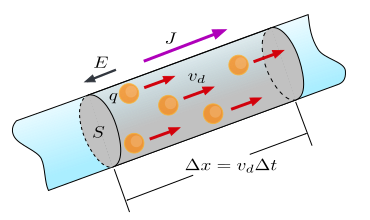
\includegraphics[width=0.5\linewidth]{el_proud_ve_vodici.pdf}
         \caption[Náboje, pohybující se vodičem]{Směr elektrického proudu byl implicitně stanoven
                  jako směr pohybu kladných nábojů. Nositeli elektrického náboje uvnitř vodičů jsou
                  ovšem záporně nabité volné elektrony, které se tedy dle  konvence pohybují proti
                  směru elektrického proudu. Elektrický proud může protékat pevnými látkami (kovy,
                  polovodiči), kapalinami (elektrolyty) a ionizovanými plyny. Látky, které nevedou
                  elektrický proud, nazýváme nevodiči, izolanty}
         \label{TEMP:fig_el_proud_ve_vodici}
      \end{figure}
      
      Elektrický proud je veličina, která obecně popisuje prostorový jev. Omezíme se nyní na běžný
      případ vodiče, jako je na obr. \ref{TEMP:fig_el_proud_ve_vodici}, který má volné náboje jen
      jedné polarity (u kovových vodičů jde o elektrony) a označme $\rho_0$ prostorovou hustotu
      volného náboje a $v_d$ velikost usměrněné rychlosti jejich nositelů (elektronů). Pak za čas
      $dt$ projde průřezem o obsahu $S_0$ ($S_0\bot v_d$) náboj $dQ = \rho_0 S_0 v_d dt$.
      Elektrický proud vyjádřený rov.
      \ref{TEMP:eq_I_01} můžeme přepsat do tvaru
        \begin{equation}\label{TEMP:eq_I_05}
          I = \rho_0 S_0 v_d = - e n_0 S_0 v_d, 
        \end{equation}         
      kde $\displaystyle{n_0 = \frac{\rho_0}{-e}}$ je počet nositelů volného náboje (tj. v našem
      případě elektronů, z nichž každý nese náboj $-e$ v jednotkovém objemu vodiče, přičemž pro
      elektrony zřejmě je $\rho_0<0$.

      \begin{wrapfigure}[14]{r}{5cm}
        \centering
        \includegraphics[width=0.9\linewidth]{plocha_S.pdf}
        \caption[Rovinná plocha $S$.]{Rovinná plocha $S = S_0\cos\alpha$}
        \label{TEMP:fig_plocha_S}
      \end{wrapfigure}
      Rovinnou plochou $S$ průřezu můžeme zavést jako vektor $vr{S}$, který má směr daný normálou k
      ploše a pravidlem pravé ruky (ukazují-li prsty pravé ruky směr oběhu po hraniční křivce
      plochy, ukáže palec směr plochy jako vektoru $\vr{S}$). Protože driftová rychlost $v_d$ je
      také vektor, nebudeme obecně uvažovat vektory $\vr{S}, \vr{v_d}$ o stejném směru a rovnici
      \ref{TEMP:eq_I_05} přepíšeme do obecnějšího tvaru      
      
      \begin{equation}\label{TEMP:eq_I_06}
        I = \rho_0 \vr{S_0}\cdot\vr{v}_d = jS\cos\alpha = jS_0, 
      \end{equation}      
      kde $S_0 = S$ pro $\alpha = 0$ (viz obr. \ref{TEMP:fig_plocha_S}) a   
      \begin{equation}\label{TEMP:eq_I_07}
        \vr{j} = \rho_0\vr{v_d}, 
      \end{equation}        
      je proudová hustota. Je to vektor o velikosti 
      \begin{equation}\label{TEMP:eq_I_08}
        j = \frac{I}{S\cos\alpha} = \frac{I}{S_0}  \qquad A\cdot m^{-2}, 
      \end{equation}   
      obecněji
      \begin{equation}\label{TEMP:eq_I_09}
        j = \frac{dI}{dS}, 
      \end{equation}

      a o směru vektoru driftové rychlosti nositelů kladného náboje. Pro případ nositelů volného
      náboje - elektronů má proudová hustota opačný směr než driftová rychlost $v_d$ (obr.
      \ref{TEMP:fig_plocha_S}).
      
      Velikost vektoru $\vr{j}$ má význam plošné hustoty elektrického proudu v uvažovaném místě
      průřezu. Jednotkou je $A\cdot m^{-2}$.
      
      Nebude-li proudová hustota na uvažovaném průřezu konstantní, bude celkový elektrický proud
      procházející průřezem o obsahu $S$ dán integrálem 
        \begin{equation}\label{TEMP:eq_I_10}
          I = \int_S \vr{j}d\vr{S}. 
        \end{equation} 

      % --------example: Driftová rychlost elektroknů ve vodiči --------
      % \label{TEO:exam008}
      % !TeX spellcheck = cs_CZ
%---------- Driftová rychlost elektroknů ve vodiči: 
\begin{mdframed}[style=mdexam]
\begin{example}\label{TEO:exam008} \emph{Driftová rychlost elektronů ve vodiči:} Vodičem z 
jednomocné mědi o
  průřezu $S_0 = \SI{1}{\mm^2}$ prochází elektrický proud $I = \SI{5}{\A}$. Vypočtěte:
  \begin{itemize}[noitemsep, leftmargin=2em]
    \item počet volných elektronů v jednotkovém objemu \ce{Cu},
    \item úhrnný náboj volných elektronů v jednotkovém objemu,
    \item driftovou rychlost volných elektronů při proudu \(I\).
  \end{itemize}
  Měď má poměrnou atomovou hmotnost $A_r = 63,54$ a hustotu\footnote{Pro hustotu budeme používat 
  alternativní značku $s$, s ohledem na kolizi značky $\rho$, jež označuje hustotu náboje.} $s = 
  \SI{8.93e3}{\kg.\m^{-3}}$.\newline  
  \textbf{Řešení:}
  \begin{itemize}[leftmargin=2em]
    \item Jeden mol mědi o molové hmotnosti $M = \SI{0.06354}{\kg\per\mol}$ a o molovém
          objemu 
          \begin{align*}
            V_m &= \frac{M}{s} 
                 = \frac{\SI{63.54e-3}{\kg.\mol^{-1}}}{\SI{8.93e3}{\kg.\m^{-3}}}      \\
                &= \SI{7.12e-6}{\m^3.\mol^{-1}}
          \end{align*}
          obsahuje $N_A = 6,0221\cdot10^{23}$ jednoatomových molekul \emph{Cu} na jeden mol,
          z nichž každý má volný jeden (valenční) elektron. Tedy počet volných elektronů v
          jednotkovém objemu je 
          \begin{align*}
            n_0 &= \frac{N_A}{V_m} = \frac{sN_A}{M}                                           
                 = \frac{\SI{6.0221e23}{\mol^{-1}}}{\SI{7.12e-6}{\m^{3}.\mol^{-1}}}    \\
                &= \SI{8.46e28}{\per\cubic\m}.
          \end{align*}  
    \item Úhrnný náboj volných elektronů v jednotkovém objemu mědi je 
          \begin{equation}
            Q_v = -e\cdot n_0 = \SI{-1.36e10}{\coulomb.m^{-3}}.
          \end{equation}
    \item Velikost driftové rychlosti určíme ze vztahu $I = -en_0v_dS_0 = - Q_v v_d S_0$ tj.
    \begin{align*}
      v_d &= \left\lvert\frac{I}{Q_v\cdot S_0}\right\rvert                       
           = \frac{\SI{5}{\coulomb\per\s}}{\SI{1.36e10}{\coulomb.m^{-3}}\cdot\SI{1e-6}{\m^2}}   \\
          &= \SI{3676e-4}{\m\per\s} = \SI{0.3676}{\mm\per\s}.  
    \end{align*}
  \end{itemize}
  Z provedených výpočtů si můžeme udělat názor o mikroskopických poměrech v kovových vodičích: počet
  volných nositelů náboje - elektronů a jejich úhrný náboj v jednotkovém objemu je značný a proto
  driftová rychlost elektronů potřebná k vyvolání proudu běžné velikosti v drátových vodičích je
  nesmírně malá (doslova hlemýždí).
\end{example}  
\end{mdframed}
  
      %-----------------------------------------------------------------

      % --------example: Velikost náboje v minci -----------------------
      % \label{TEO:exam009}
      % !TeX spellcheck = cs_CZ
%---------- Velikost náboje v minvi:
\begin{example}
  Elektricky neutrální měděná mince o hmotnosti \(m = \SI{3.11}{\g}\) obsahuje stejné množství 
  kladného a záporného náboje. Jaké je velikost kladného (nebo záporného) náboje obsaženého v 
  minci?\newline  
  \textbf{Řešení:}\newline
  Neutrální atom má záporný náboj \(Z\cdot e\), představovaný jeho elektrony a kladný náboj o 
  stejné velikosti představovaný protony v jádře. Pro měď je atomové číslo \(Z\) rovno \num{29}, 
  tj. atom mědi má \num{29} protonů, a je-li elektricky neutrální, také \num{29} elektronů.
  
  Náboj o velikosti \(Q_v\), který hledáme je roven \(N\cdot Z\cdot e\), kde \(N\) je počet atomů 
  obsažených v  jednom molu (Avogadrova konstanta: \(N_A = \SI{6.0221e23}{\per\mole}\)). Počet 
  molů mědi v minci \(\frac{m}{M}\), kde \(M = \SI{63.5}{\g\per\mole}\) je molární hmotnosti mědi: 
  \begin{equation*}
    N = N_A\cdot\frac{m}{M} = \SI{6.0221e23}{\per\mole}
           \frac{\SI{3.11}{\g}}{\SI{63.5}{\g\per\mole}} 
      = \num{2.95e22}.
  \end{equation*}
 Velikost celkového kladného (záporného) náboje v minci je pak 
  \begin{equation*}
    Q_v = N\cdot Z\cdot e = \num{2.95e22}\cdot\num{29}\cdot\SI{1.602e-19}{\coulomb} 
        = \SI{137039}{\coulomb}
  \end{equation*}
  To je obrovský náboj. Pro srovnání: třeme-li ebonitovou tyč vlněnou látkou, můžeme na tyč 
  přemístit stěží náboj o velikosti \SI{1e-9}{\coulomb}.
\end{example} 
  
      %-----------------------------------------------------------------

    % ----------------Práce a výkon elektrického proudu-----------------
    \subsection{Práce a výkon elektrického proudu}
      % --------example: Ponorný vařič ---------------------------------
      % \label{TEO:exam010}
      % !TeX spellcheck = cs_CZ
%---------- Ponorný vařič:
\begin{mdframed}[style=mdexam]
  \begin{example}\label{TEO:exam010}
    Za jakou dobu uvede norný vodič o příkonu \SI{600}{\W} do varu \SI{1}{\litre} vody o počáteční
    teplotě $\SI{20}{\degreeCelsius}$. Uvažujte měrnou tepelnou kapacitu vody $c =
    \SI{4200}{\joule\per\kg\per\K}$. Výměnu tepla s okolím neuvažujte.
    \newline 
    \textbf{Řešení:}\newline Pro var vody bude zapotřebí tepla dle rovnice $Q  = m\cdot c\cdot(T_2 -
    T_1)$. Potřebná elektrická práce je $Q_e = P\cdot t = U\cdot I\cdot t$ a tedy dobu ohřevu
    stanovíme z rovnice:
    
    {\centering
    \captionsetup{type=figure}
    \luafigure[0.3]{teo_fig033.png}
    \captionof{figure}{Ilustrace k příkladu \ref{TEO:exam010}}
    \label{teo:fig033}
    \par}

    \begin{align*}
      P\cdot t &= m\cdot c\cdot(T_2 - T_1)                                               \\
             t &= \frac{m\cdot c}{P}\cdot(T_2 - T_1)                                     \\     
               &= \frac{\SI{1}{\kg}\cdot\SI{4200}{\joule\per\kg\per\K}}{\SI{600}{\W}}
                \cdot(\SI{100}{\degreeCelsius} - \SI{20}{\degreeCelsius})                \\ 
               &= \SI{560}{\s}.
    \end{align*}         
  \end{example}
\end{mdframed}  
      %-----------------------------------------------------------------
 
    % ----------------Ohmův zákon------------------------------------------------------------------
    \subsection{Ohmův zákon}
      Uvažujme vodič u něhož jsou volnými nositeli náboje \emph{elektrony}. Nyní v mezích klasické
      mechaniky kvantitativně popíšeme mechanismus vedení proudu, který povede k všeobecně známému
      \textbf{Ohmovu zákonu}
      
      Umístíme-li vodič do elektrického pole o intenzitě $\vec{E}$ (např. připojením ke
      galvanickému článku), působí na každý volný elektron síla $\vec{F} = -e\vec{E}$, která mu
      podle \emph{Newtonova zákona} udělí zrychlení $\vec{a} = \frac{\vec{F}}{m_e} = -
      \frac{e}{m_e}\vec{E}$ proti směru vnějšího pole. Tím získávají chaoticky se pohybující
      elektrony ještě složku rychlosti v protisměru vloženého elektrického pole $\vec{E}$ a  dojde
      tedy k usměrnění driftového pohybu volných elektronů a v souladu s kapitolou
      \ref{TEMP:kap_elproud_jev} pozorujeme, že ve vodiči vznikl makroskopický elektrický proud.
      
      Pohyb elektronu se ovšem neobejde bez srážek s ionty v krystalové mřížce. Dráhu, kterou se
      elektronu podaří urazit, nazýváme \emph{volnou dráhou} $d$. Průměrná doba mezi dvěma po sobě
      jdoucími srážkami nechť je $\tau$ za tuto dobu se bude elektron rovnoměrně urychlovat a těsně
      před následující srážkou jeho rychlost dosáhne maxima tj. $\vec{v}_{max} = \vec{a}\cdot\tau$.
      Nás ovšem zajímá průměrná rychlost (\emph{driftová rychlost})na volné dráze průměrné
      velikosti:
      \begin{equation}\label{TEMP:eq_vd_01}
        \vec{v}_d = \frac{\vec{v}_{max}}{2} = -\frac{e\tau}{2m_e}\vec{E}
      \end{equation}   
      Proudová hustota \ref{TEMP:eq_I_07} bude
      \begin{equation}\label{TEMP:eq_j_02}
        \vec{j} = \rho_0\vec{v}_d= -en_0\vec{v}_d = -\frac{e^2n_0\tau}{2m_e}\vec{E}
      \end{equation}       
      Koeficient úměrnosti 
      \begin{equation}\label{TEMP:eq_g_03}
        \gamma = \frac{e^2n_0\tau}{2m_e}
      \end{equation}     
      je závislý na počtů nositelů (elektronů) $n_0$ v jednotkovém objemu a na době $\tau$, neboli
      na délce volné dráhy. Veličina $\gamma$ se nazývá \emph{měrná elektrická vodivost} neboli
      \textbf{konduktivita} látky. Protože dobu $\tau$ nelze přímo měřit, určuje se $\gamma$
      experimentálně. Přitom se zjišťuje, že pro určitou teplotu zkoumané látky je $\gamma$
      konstantní.
      
      Po zavedení pojmu měrná elektrická vodivost látky \ref{TEMP:eq_g_03}, můžeme výraz
      \ref{TEMP:eq_j_02} přepsat do výsledného tvaru
      \begin{equation}\label{TEMP:eq_j_04}
        \vec{j} = \gamma\vec{E},
      \end{equation}              
      který se v literatuře označuje jako \emph{Ohmův zákon v diferenciálním tvaru} (i když se v
      pravém slova smyslu o diferenciální tvar nejedná). Výstižnější je označení \emph{lokální tvar
      Ohmova zákona}, protože výraz \ref{TEMP:eq_j_04} se vztahuje na určité místo, resp. bod,
      vodivého prostředí. Vztah říká, že proudová hustota v určitém bodě vodivého prostředí je
      přímo úměrná intenzitě vloženého elektrického pole v tomto bodě (platí pro určitou teplotu
      prostředí).
      
      Uvažujme nyní lineární homogenní vodič délky $l$ a příčného průřezu o obsahu $S_0$, připojený
      ke zdroji o napětí $U$. Pak intenzita pole uvnitř vodiče bude mít konstantní velikost
      $E=\frac{U}{l}$. Dosadíme-li za velikost proudové hustoty $j=\frac{I}{S_0}$ do
      \ref{TEMP:eq_j_04}, dostaneme vztah
      \begin{equation}\label{TEMP:eq_j_05}
        \frac{I}{S_0} = \gamma\frac{U}{l},
      \end{equation}        
      z něhož vyplývá známý vztah
      \begin{equation}\label{TEMP:eq_j_06}
        U = \frac{l}{\gamma S_0}I = RI,
      \end{equation}              
      kde
      \begin{equation}\label{TEMP:eq_j_07}
        R = \frac{l}{\gamma S_0} = \rho\frac{l}{S_0},
      \end{equation} 
      je \textbf{elektrický odpor} uvažovaného lineárního vodiče, přičemž $\rho = \frac{1}{\gamma}$
      je \emph{měrný elektrický odpor} (\textbf{rezistivita})\footnote{Zde je další kolize značky
      $\rho$. Nyní se tomuto problému vyhneme využíváním pouze konduktivity, jenž se častěji
      používá v teorii elektromagnetického pole.}. Výraz \ref{TEMP:eq_j_07} představuje klasický
      Ohmův zákon zákon experimentálně objevený r. 1826 \emph{G. S. Ohmem}. Jednotky:
      \begin{itemize}\addtolength{\itemsep}{-0.5\baselineskip}
        \item elektrický odpor: \si{V.A^{-1}},
        \item měrný elektrický odpor: \si{\ohm.m},
        \item měrná elektrická vodivost: \si{\ohm^{-1}.m^{-1}}.
      \end{itemize}

      % --------example: Ponorný vařič -----------------------
      % \label{TEO:exam011}
      % !TeX spellcheck = cs_CZ
\begin{example}
  \textbf{Zemnicí elektroda}: Uvažujte zemnicí elektrodu ve tvaru koule o poloměru  
  $a=\SI{200}{\mm}$, uloženou do zeminy v hloubce, která je značně větší než je poloměr $a$. Pro 
  jednoduchost řešení dále předpokládejte, že přívodní drát je od zeminy izolován (obr.
  \ref{TEMP:fig_zem_elektroda}). Zemina má měrnou vodivost $\gamma=\num[exponent-product =
  \cdot]{1,8e-2}\si{\per\ohm\per\m}$. Při zkratu teče přívodním drátem proud $I=\SI{50}{\A}$.
  Vypočítejte:
  
  %----------------------------------
  % image: TEMP_zem_elektroda.tex label: \label{TEMP:fig_zem_elektroda}
  \input{../src/TEO/img/TEMP_zem_elektroda.tex}  
  %----------------------------------         
  \begin{enumerate}[label=\emph{\alph*})]
    \item Závislost potenciálu $\varphi=\varphi(r)$ elektrického pole, které se vytvoří v
          zemině při zkratu, kde $r$ je vzdálenost od středu elektrody. Potenciál normujte
          volbou $\varphi(\infty)=0$.
    \item Zemnicí odpor elektrody, který je definován vztahem $$R_z=\frac{U_z}{I_z},$$ kde
          $U_z = \varphi(a)-\varphi(b)$ je zemnicí napětí 
    \item Ztrátový výkon při zkratu.            
  \end{enumerate}
  Řešení:    
  Ekvipotenciální a proudové plochy mají zřejmě kulový tvar se středem totožným s geometrickým 
  středem elektrody. Proudová hustota na kulové ploše obecného poloměru $r$ (viz. obr. 
  \ref{TEMP:fig_zem_elektroda}) je $$\vec{j}=\frac{I}{4\pi r^2}\vec{n},$$ kde $\vec{n}$ je 
  jednotkový vektor ve směru normály. Pak v bodech na této ploše musí být elektrické pole o 
  intenzitě $\vec{E}$, kterou určíme ze vztahu
  \begin{equation*}
    \vec{j}= \gamma\vec{E}\rightarrow\vec{E}=
    \frac{\vec{j}}{\gamma}=\frac{I}{4\pi\gamma r^2}\vec{n}.
  \end{equation*}
  Závislost potenciálu $\varphi=\varphi(r)$ tohoto elektrického pole stanovíme pomocí následujícího 
  integrálu
  \begin{equation}
    \varphi = - \int\vec{E}d\vec{r}+C = -\frac{I}{4\pi\gamma}\int\frac{dr}{r^2} + C 
            =   \frac{I}{4\pi\gamma r} + C, \nonumber
  \end{equation} 
  kde integrační konstantu $C$ určíme z okrajové podmínky $\varphi(\infty)=0$, odkud $C=0$.
  Hledaná závislost potenciálu je
  \begin{equation*}
    \varphi = \frac{I}{4\pi\gamma r}, \qquad r\in\langle a, \infty). 
  \end{equation*}           
  
  Zemina, v níž je uložena elektroda, je vlastně rezistorem, jehož jeden okraj tvoří elektrodu
  a druhým okrajem je nekonečně rozlehlý vodivý prostor. Potenciální rozdíl mezi těmito okraji je
  \begin{equation*}
    U_z = \varphi(a) - \varphi(\infty)= \frac{I}{4\pi\gamma a},
  \end{equation*} 
  \begin{minipage}[t]{0.5\textwidth}% first column            
    odkud zemnicí odpor 
    \begin{equation*}
      R_z = \frac{U_z}{I} = \frac{1}{4\pi\gamma a} = \SI{22,1}{\ohm}
    \end{equation*}
  \end{minipage}
  \begin{minipage}[t]{0.5\textwidth}% second column    
    a ztrátový výkon 
    \begin{equation*}
      P_z = R_z\cdot I^2 = \SI{55,3}{\kilo\watt}. 
    \end{equation*}
  \end{minipage}
\end{example}


  
      %-------------------------------------------------------

    % ------------------- Elektromotorické napětí -------------------------------------------------
    \subsection{Elektromotorické napětí}
      Uzavřený proudový okruh $C$, nechť je v dynamické rovnováze - prochází jím ustálený
      elektrický proud. Uvažujme pro jednoduchost představy kladný náboj - ten se musí pohybovat ve
      směru klesajícího potenciálu (záporný náboj ve směru stoupajícího potenciálu). Je-li okruh
      uzavřený, musí kladné náboje opět vystoupit na místo s vyšším potenciálem - musí se tedy
      pohybovat proti elektrostatickým silám. Proto proti úbytku      
               
  % ----------------Stacionární magnetické ole-----------------------------------------------------
  \newpage
  \section{Stacionární magnetické pole}
    Zdrojem stacionárního magnetického pole jsou stejnosměrné proudy nebo permanentní magnety.
    Základní rovnice stacionárního magnetického pole jsou:

    \begin{table}[ht!]
      \centering
      \begin{tabular}{lc|c|}
        \cline{2-3}
        \multicolumn{1}{l|}{} & \textbf{integrální tvar} & \textbf{diferenciální tvar} \\
        \hline
        \multicolumn{1}{|l|}{1. MR} & $\oint\vr{H}\cdot d\vr{l} = I$ & $\rot{H} = \vr{J}$ \\ 
        \cline{1-3}
        \hline
        \multicolumn{1}{|l|}{4. MR} & $\oint\vr{B}\cdot d\vr{S} = 0$ & $\diver{B} = 0$ \\
        \cline{1-3}
        & & $\vr{B} = \mu \vr{H}$ \\
        \cline{3-3}
      \end{tabular}
      \caption{Základní rovnice magnetického stacionárního pole}
    \end{table}

    Směr vektoru $\vr{H}$ se prakticky určí například \emph{pravidlem pravotočivého šroubu}: vodič
    nahradíme šroubem (s pravotočivým závitem) a otáčíme jím tak, aby se pohyboval ve směru proudu;
    směr otáčení pak udává směr vektoru $\vr{H}$. Vše je názorně vysvětleno na obrázku
    \ref{temp:fig_pravidlo_sroub}. Podobných pomůcek existuje více, např. \emph{pravidlo pravé
    ruky}: vodič uchopíme do dlaně pravé ruky tak, aby palec ukazoval směr proudu; prsty pak
    ukazují směr vektoru $\vr{H}$, obr. \ref{temp:fig_pravidlo_ruka}.

         \begin{figure}[ht!]
           \centering
           \subfloat[Pravidlo pravé ruky]{\label{temp:fig_pravidlo_ruka}
             \includegraphics[width=0.4\linewidth]{pravidlo_prave_ruky.pdf}}
           \hspace{2cm}
           \subfloat[Pravidlo pravotočivého šroubu]{\label{temp:fig_pravidlo_sroub}
             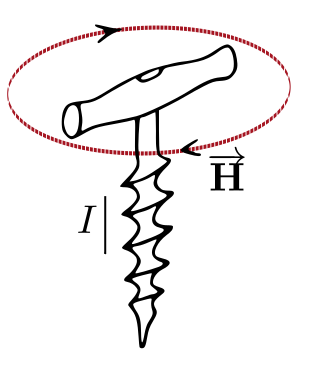
\includegraphics[width=0.3\linewidth]{pravidlo_pravotociveho_sroubu.pdf}}
           \caption[Pravidlo pravé ruku a pravotočivého šroubu]{Určení směru vektoru $\vr{H}$: a)
                   pravidlem pravé ruky; b) pravidlem pravotočivého šroubu}
           \label{temp:fig_urceni_H}
         \end{figure}
    K procvičení těchto pravidel je na obr. \ref{TEMP:fig_ind_c_kruh_z} vyznačen směr indukčních
    čar kruhové\-ho závitu. Označení $\bigotimes$ vyjadřuje proud vstupující  do nákresny (symbol
    letícího šípu od pozorovatele) a označením $\bigodot$ proud vystupující z nákresny (symbol
    hrotu šípu).
    
    \begin{figure}[ht!]
      \centering
      \includegraphics[width=0.4\linewidth]{mag_ind_cary_kruh_z.pdf}
      \caption{Indukční čáry kruhového závitu.}
      \label{TEMP:fig_ind_c_kruh_z}
    \end{figure}    
    Rovnice \ref{TEMP:eq_zak_celk_I} představuje \textbf{zákon celkového proudu} vyjadřující,
    rovnost oběhového magnetické napětí na libovolné uzavřené orientované křivce $c$ proudu, který
    je s křivkou $c$ spřažen. ''\emph{Spřaženým proudem}'' rozumíme proud, který prochází 
    libovolnou plochou $S$, jež je ohraničená křivkou $c$, přičemž plocha $S$ je orientována vůči 
    křivce $c$ pravotočivě (obr. \ref{TEMP:fig_1MR_pic}). \cite[s.~55]{Mayer2001}.

      \begin{equation}\label{TEMP:eq_zak_celk_I}
        \oint\vr{H}\cdot d\vr{l} = I   
      \end{equation}    
     
      \begin{figure}[ht!]
         \centering
         \includegraphics[width=0.7\linewidth]{1MR_pic.pdf}
         \caption[Zákon celkového proudu]{K zákonu celkového proudu}
         \label{TEMP:fig_1MR_pic}
      \end{figure}

         \begin{figure}[hb!]
           \centering
           \subfloat[$\oint\vr{H}\cdot d\vr{l} = 0$]{\label{TEMP:fig_mag_sprazeny_proud1}
             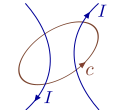
\includegraphics[width=0.3\linewidth]{mag_sprazeny_proud1.pdf}}
           \subfloat[$\oint\vr{H}\cdot d\vr{l} = 0$]{\label{TEMP:fig_mag_sprazeny_proud2}
             \includegraphics[width=0.3\linewidth]{mag_sprazeny_proud2.pdf}}
           \subfloat[$\oint\vr{H}\cdot d\vr{l} = 3I$]{\label{TEMP:fig_mag_sprazeny_proud3}
             \includegraphics[width=0.3\linewidth]{mag_sprazeny_proud3.pdf}}             
           \caption[K pojmu ''proud spřažený s křivkoku'']{K pojmu ''proud spřažený s křivkoku''
                    pro tři různé případy křivky $c$.}
           \label{TEMP:fig_mag_sprazeny_proud123}
         \end{figure}
         
    Základní úlohou řešení stacionárních proudových magnetických polí je určení rozložení veličin 
    $\vr{H}$ a $\vr{B}$ v prostoru, je-li dáno prostorové a materiálové uspořádání a elektrické 
    proudy vybuzují řešené magnetické pole.
    
    V následujících úlohách se omezíme na analýzu jednodušších, souměrných magnetických polí v 
    lineárním izotropním alespoň po částech homogenním prostředí. Pro zjednodušení budeme 
    zanedbávat deformaci magnetického pole v okrajových oblastech a nebudeme uvažovat vliv 
    blízkosti nesymetrického rozhraní a vliv blízkosti druhého zdroje magnetického pole. (Pro 
    přesnější řešení by pak bylo nutné použít tzv. \emph{metodu zrcadlení}.) Některá složitější 
    pole lze rozdělit na několik jednodušších polí souměrného charakteru, resp. typického 
    uspořádání. Vzhledem k tomu, že v předpokládaném lineárním prostředí ($\mu 
    = konst$) platí pro stacionární magnetické pole \emph{princip superpozice}, lze samostatně 
    vyřešit nejprve dílčí jednodušší pole jednotlivých proudů $I_j$ a po jejich superpozici
      \begin{equation}\label{TEMP:eq_superp_mag_pole}
        \vr{H}= \sum_{j=1}^n\vr{H}_j(I_j), \quad\text{resp.}\quad \vr{B}= 
        \sum_{j=1}^n\vr{B}_j(I_j)   
      \end{equation}
    získáme výsledné pole celkového proudu \cite[s.~181]{Kotlan1999}. 
    
    Metodou přímé aplikace I. Maxwellovy rovnice v integrálním tvaru pro stacionární magnetické
    pole proudové
      \begin{equation}\label{TEMP:eq_1MR_rozbor}
        \oint_\mathcal{C}\vr{H}d\vr{l} = \oint_\mathcal{C}H\cos\alpha dl = I_c
      \end{equation}    
    lze jednoduše použít tehdy, je-li ze zadané úlohy zřejmá taková symetrie pole, že lze z 
    nekonečně mnoha uzavřených křivek, splňující rov. \ref{TEMP:eq_1MR_rozbor}, nalézt takovou 
    integrační dráhu $c$, která obepíná proud $I_c$ vytvářející magnetické pole a v jejichž bodech 
    platí podmínka
      \begin{equation}\label{TEMP:eq_H_alpha_konst}
        H = \text{konst}, \qquad \alpha = \text{konst},
      \end{equation}    
    speciálně
      \begin{equation}\label{TEMP:eq_alpha_0}
        H = \text{konst}, \qquad \alpha = 0.
      \end{equation}
    
    Podmínka $\alpha = 0$, tj. $\vr{H}\| d\vr{l}$ je identicky splněna na siločáře magnetického 
    pole. Siločáry souměrných stacionárních magnetických polí splňují tedy podmínku 
    \ref{TEMP:eq_alpha_0} a řešení rovnice \ref{TEMP:eq_1MR_rozbor} při integraci po takovéto 
    siločáře je jednoduché
      \begin{equation}\label{TEMP:eq_1MR_alpha0}
        \oint_\mathcal{C}\vr{H}d\vr{l} = H\underbrace{\oint_\mathcal{C} dl}_{l_c} = 
                                         I_c \rightarrow H = \frac{I_c}{l_c}
      \end{equation}            
    kde $l_c$ je délka integrační dráhy $c$ splňující podmínku \ref{TEMP:eq_alpha_0}.
      
    Klasickým případem takovéto úlohy je magnetické pole \emph{dlouhého přímého válcového vodiče} o
    poloměru $a$, délky $l$ protékaného proudem $I$ rozloženým po průřezu souměrně kolem osy 
    vodiče, tzn, obecně s hustotou $J = J(r)$. Z osové (rotační) symetrie vyplývá, že siločáry 
    magnetického pole mají tvar soustředných kružnic se středem v ose vodiče, ležících v rovině 
    kolmé na osu vodiče obr. \ref{TEMP:fig_mag_pole_vodic_I_konst}.
    \begin{figure}[ht!]
      \centering
      \includegraphics[width=0.7\linewidth]{mag_pole_vodic_I_konst.pdf}
      \caption[Pole dlouhého dutého vodiče protékaného konstantním proudem]{Pole dlouhého dutého
               vodiče protékaného konstantním proudem}
      \label{TEMP:fig_mag_pole_vodic_I_konst}
    \end{figure}        
    Úlohy proto řešíme ve válcových souřadnicích s osou $z$ totožnou s osou vodiče. Za 
    předpokladu, že průměr vodiče je zanedbatelný vůči jeho délce lze zanedbat deformaci pole 
    vlivem konců válcového vodiče a přejít na rovinný problém v polárních souřadnicích. Z důvodu 
    osové  souměrnosti je však pole závislé jen na vzdálenosti $r$ od osy vodiče tj. $$H = H(r), 
    \qquad B = B(r).$$ Na kruhových siločárách je tedy splněna podmínka \ref{TEMP:eq_alpha_0} a z 
    I. Maxwellovy rovnice \ref{TEMP:eq_1MR_rozbor} 
      \begin{equation}\label{TEMP:eq_1MR_rozbor2}
        \oint_{\mathcal{C}}\vr{H}d\vr{l} = H\cos0\oint_\mathcal{C}dl = I(r),
      \end{equation}     
    kde $c$ je kružnice o poloměru $r$ a proud $I(r)$ je dán rovnicí
      \begin{equation}\label{TEMP:eq_1MR_Ir}
        I(r) = \int_{S(r)}\vr{J}(r)d\vr{S} = \int_0^rJ(r)2\pi rdr
      \end{equation}           
    je proud protékající přes kruhovou plochu $S(r)$ ohraničenou kružnicí o poloměru $r$. Pak
    intenzita magnetického pole ve vzdálenosti $r$ od osy vodiče má velikost
      \begin{equation}\label{TEMP:eq_Hr_vodice}
        H = H(r) = \frac{I(r)}{2\pi r},
      \end{equation}       
    a magnetická indukce 
      \begin{equation}\label{TEMP:eq_Br_vodice}
        B = B(r) = \frac{\mu I(r)}{2\pi r},
      \end{equation}       
    přičemž $\mu$ je \emph{permeabilita} v bodech na poloměru $r$. Magnetické pole v okolí
    kruhové\-ho přímého vodiče protékaného proudem $I$ viz obr. \ref{teo:fig021} je tedy v souladu 
    s předchozími úvahami dáno výrazy \cite[s.~183 - 185]{Kotlan1999}:
    \begin{figure}[ht!]
      \centering
      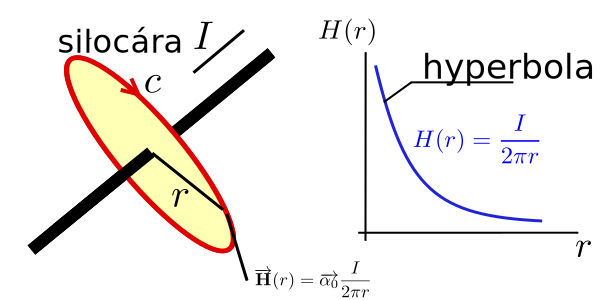
\includegraphics[width=0.8\linewidth]{teo_fig021.pdf}
      \caption[Průběh intenzity magnetického pole dlouhého dutého vodiče protékaného konstantním
               proudem]{Průběh intenzity magnetického pole dlouhého dutého vodiče protékaného
               konstantním proudem}
      \label{teo:fig021}
    \end{figure}      
      \begin{equation}\label{TEMP:eq_Hr_Br_vodice}
        H = H(r) = \frac{I}{2\pi r}, \qquad B = B(r) = \frac{\mu I}{2\pi r}.
      \end{equation}   
    Jelikož 1. MR má nenulovou pravou stranu v magnetickém poli obecně není splněna nutná a
    postačující podmínka, aby magnetické napětí
      \begin{equation}\label{TEMP:eq_mag_napeti}
        \int_{M(l)}^N\vr{H}d\vr{l} = U_{m_{MN}} \qquad [A]
      \end{equation}       
    nezáviselo na tvaru integrační cesty $l$ z $M$ do $N$. Tedy obecně nelze zavést \emph{skalární
    magnetický potenciál}. Magnetické pole je tedy obecně \textbf{vírové (nepotenciální)}.

    Všimněme si však speciálních případů, kdy pravá strana 1. MR je nulová a tedy magnetické pole
    bude \textbf{nevírové (magnetostatické)}. K tomu dochází buď v oblasti kde 
      \begin{equation}\label{TEMP:eq_1MR_0}
        \oint_{\mathcal{C}}\vr{H}d\vr{l} = 0
      \end{equation}    
    tj. takové v němž neexistuje uzavřená křivka $c$ spřažená s nějakým proudem, nebo v takovém
    bodu, v němž platí
      \begin{equation}\label{TEMP:eq_rotH_0}
        \rot{\vr{H}} = 0
      \end{equation}
    tj. v bodu v němž je $\vr{J} = 0$.
    
    Analogicky jako v elektrostatice, lze pak zavést magnetický potenciál $\varphi_m$ vztahem  
      \begin{equation}\label{TEMP:eq_grad_varphi_m}
        \vr{H} = - \grad{\varphi_m}.
      \end{equation}              
    Jednotkou $\varphi_m$ je \emph{ampér} [A]. Pro magnetické napětí mezi body $M, N$ platí
    analogicky
      \begin{equation}\label{TEMP:eq_Umn_def}
        U_{MN} = \int_{M(l)}^N\vr{H}d\vr{l} = \varphi_m(M) - \varphi_m(N),
      \end{equation}        
    nezávisle na integrační cestě $l$. 
     
    % ----------------Magnetické pole vodičů s proudem v homogenním izotropním prostředí ----------
    \subsection{Magnetické pole vodičů s proudem v homogen\-ním izo\-trop\-ním prostředí}
      Z předchozí kapitoly vyplývá, že intenzitu magnetického pole $\vr{H}$ lze stanovit pomocí
      vztahu $\oint\vr{H}\cdot d\vr{l} = I$ tehdy, víme-li předem, že daným bodem prochází silová
      čára, na níž je intenzita pole konstantní, $H_s = \text{konst}$. V tomto případě se křikový
      integrál změní v pouhý součin intenzity pole a délky silové čáry
       
       \begin{equation}\label{TEMP:eq_1MR_v_hom_p}
         \oint_\mathcal{C}\vr{H}d\vr{l} = H_s\oint_\mathcal{C}\vr{l} = H_s\cdot l_s
       \end{equation}      
       
      takže lze vypočítat intenzitu pole $$H_s = \frac{I}{l_s}$$ pro body silové čary. 
      
      Tohoto postupu lze použít i tam, kde uvedená podmínka není splněna, avšak pole lze vyjádřit
      superpozicí dílčích polí, z nich každé tuto podmínku splňuje, viz příklad 
      \ref{TEMP:ex_koax_H}. 

      % --------example: $H=f(r)$ dlouhého dutého válcového vodiče ------
      % \label{TEO:exam012}
      % !TeX spellcheck = cs_CZ
\begin{example}
  Stanovte intenzitu magnetického pole $H=f(r)$ dlouhého dutého válcového vodiče podle obr.
  \ref{TEMP:fig_pole_duty_valec} při rovnoměrném rozložení proudu $I$ po průřezu. 
  
   {\centering
    \captionsetup{type=figure}
    \includegraphics[width=0.6\linewidth]{duf_duty_valec_H.pdf}
    \captionof{figure}{K příkladu stanovení intenzity magnetického pole dlouhého dutého válcového 
               vodiče protékaného proudem}
    \label{TEMP:fig_pole_duty_valec}
  \par}
  
  Vodič s rovnoměrně rozloženým proudem podle obr. \ref{TEMP:fig_pole_duty_valec} je rotačně
  souměrný podle své osy a tedy i jeho magnetické pole je souměrné. Silové čáry jsou soustředné
  kružnice, vektor $\vr{H}$, jenž má směr tečny ke kružnici, je po celé délce kružnice stejně
  velký. Lze tedy snadno použít integrálního tvaru 1. MR (\textbf{zákon celkového proudu})
  
  Pro body ležící vně vodiče obepíná kruhová integrační dráha (vedená po silové čáře 1) celý
  proud vodiče $I$ a platí
  \begin{equation}\label{TEMP:eq_1MR_duty_valec}
    \oint_\mathcal{C}\vr{H}d\vr{l} = H\cdot 2\pi r = I
  \end{equation}
  takže intenzita pole je
  \begin{equation}\label{TEMP:eq_H_duty_valec}
    H = \frac{I}{2\pi r}
  \end{equation}
  
  Ve stěně dutého magnetického vodiče jsou silové čáry rovněž kružnice, neboť magnetické pole
  je i zde souměrné. Tyto siločáry však obepínají jen část proudu $I'$ vodiče pro oběh siločáry
  2 platí
  \begin{equation}\label{TEMP:eq_1MR_uvnitr_valce}
    \oint_\mathcal{C}\vr{H}d\vr{l} = H\cdot 2\pi r = I' = \pi(r^2-r_1^2)J
  \end{equation}
  kde $J$ je hustota proudu ve vodiči
  \begin{equation}\label{TEMP:eq_J_duty_valec}
    J = \frac{I}{S}= \frac{I}{\pi(r_2^2-r_1^2)}
  \end{equation}
  Ve stěně vodiče je tedy intenzita pole
  \begin{equation}\label{TEMP:eq_H_uvnitr_valce}
    H = \frac{I}{2\pi r}\frac{r^2-r_1^2}{r_2^2-r_1^2}
  \end{equation}
  V dutině vodiče je intenzita rovna nule. Vzhledem k souměrnosti pole by i zde muselo platit
  $\oint_\mathcal{C}\vr{H}d\vr{l} = H\cdot 2\pi r$. Protože dráha s poloměrem $r<r_1$ neobepíná
  žádný proud, je $\oint_\mathcal{C}\vr{H}d\vr{l} = 0$ a tedy musí byt $H = 0$.
\end{example}    
  
      %------------------------------------------------------------------

      % --------example: $H=f(r)$ souosého kabelu -----------------------
      % \label{TEO:exam013}
      % !TeX spellcheck = cs_CZ
\begin{mdframed}[style=mdexam]
  \begin{example}\label{TEMP:ex_koax_H}
    Stanovte intenzitu magnetického pole dlouhého přímého souosého kabelu podle obr.
    \ref{teo:fig066}. Středním vodičem (\emph{žílou}) prochází proud $I$ a týž proud
    opačného smyslu prochází vnějším vodičem (\emph{pláštěm}). Proudy jsou rovnoměrně rozloženy po
    průřezech vodičů. Nakreslete graf průběhu $H = f(r)$ \cite[s.~92]{Dufek1970},
    \cite[s.~195]{Kotlan1999}.
    
    {\centering
    \luafigure[0.45]{teo_fig066a.pdf}     \hspace{1em}
    \luafigure[0.45]{teo_fig066b.pdf}
    \captionsetup{type=figure}  
    \captionof{figure}{K příkladu stanovení intenzity magnetického pole dlouhého souosého kabelu
      protékaného proudem: a) náčrt; b) $H=f(r)$}           
    \label{teo:fig066}
    \par}
 
    \textbf{Řešení}: \newline Rovnici \ref{TEMP:eq_1MR_v_hom_p} aplikujeme na jednotlivé intervaly
    osově souměrného stacionárního magnetického pole, přičemž se prakticky jedná o superpozici dvou
    polí. V oblasti $r<r_2$ se uplatňuje pouze pole vnitřního válcového vodiče (žíly), pro $r>r_2$
    přistupuje souosé pole vnějšího trubkového vodiče.
    \begin{itemize}
      \item Pro oblast $r<r_1$ je vzhledem k 
            \begin{align*}
                % \nonumber to remove numbering (before each equation)
                \dd{I}&= \vr{J}d\vr{S} \\
                I(r)  &= \int_S dI = \int_S \vr{J}d\vr{S} = \int_S J\cos\beta dS \\
                      &= \left\lvert\begin{array}{cc}
                                \beta = 0 & H = \text{konst}   \\
                              S = \pi r^2 & dS = 2\pi r\dd{r}  \\
                              \end{array}
                        \right\rvert                                           \\
                      &= J\int_0^r 2\pi rdr = J\pi r^2
            \end{align*}
            hledané řešení 1. MR dáno 
            $$\oint_{\mathcal{c}}\vr{H}d\vr{l} = H_1 2\pi r = I(r) = J\pi r^2$$ kde celková proudová
            hustota je  $$J = \frac{I}{\pi r_1^2}$$ a tedy
            $$H_1 = \frac{I}{2\pi r_1^2}\cdot r$$
            
      \item Pro oblast $r_2>r>r_1$ řešíme v podstatě pole vně osamoceného válcového vodiče $I(r)$ a
            tedy $$H_2 = \frac{I}{2\pi r}$$
      \item Pro $r>r_3$ je magnetické pole vytvářeno celým proudem žíly $I$ a příslušnou částí
            proudu pláště $J\pi(r^2 - r_2^2)$, kde proudová hustota $$J =
            \frac{I}{\pi(r_3^2-r_2^2)}$$ má opačnou orientaci oproti proudové hustotě žíly. Pak 
            \begin{align*}
              I(r)                             &= I - I\frac{r^2-r_2^2}{r_3^2-r_2^2} \\
              \oint_{\mathcal{c}}\vr{H}d\vr{l} &= H_32\pi r = I(r)                   \\          
              H_3                              &= \frac{I}{2\pi r}\left(1 - 
              \frac{r^2 - r_2^2}{r_3^2 - r_2^2}\right) 
            \end{align*}
            Stejný výsledek dostaneme superpozicí opačně orientovaných polí
            $$H_3 = H'_3 - H''_3 = \frac{I}{2\pi r} - \frac{I}{2\pi r}\left(\frac{r^2 - r_2^2}{r_3^2
            - r_2^2}\right)$$. 
    \end{itemize}
    Průběh $H(r)$ je na obr. \ref{teo:fig066}.
  \end{example}
\end{mdframed}  
      %------------------------------------------------------------------

    % -----------Magnetické pole elektrického proudu v diferenciálním tvaru-----------------------
    \subsection{Magnetické pole elektrického proudu v diferenciálním tvaru}
      Nechť je opět magnetické pole vyvoláno konstantním el. proudem $I = \text{konst}$. Jak
      vyplývá z předchozí kapitoly, základním vztahem pro toto pole je \emph{Ampérův zákon}
      $$\oint_\mathcal{c}\vr{H_c}d\vr{l} = I$$  Zvolme za integrační dráhu $c$ obvod malé plošky
      $\Delta S$, jíž prochází proud $\Delta I = J_n \Delta S$, kde $J_n$ je průmět vektoru hustoty
      proudu do směru normály plošky $\Delta S$ (předpokládáme, že ploška $\Delta S$ je dostatečně
      malá, aby se dalo počítat s konstantní hustotou proudu v celém jejím rozsahu)
      \cite[s.~13]{Trnka1972}. Pro zvolený případ platí
      
      \begin{equation}\label{TEMP:eq_amp_z1}
        \oint_\mathcal{c}\vr{H_c}d\vr{l}  =
           J_n \Delta S \rightarrow \frac{1}{\Delta S}\oint_\mathcal{c}\vr{H_c}d\vr{l} = J_n
      \end{equation} 
      
      Pro $\Delta S \rightarrow 0$ zavedeme označení 
      \begin{equation}\label{TEMP:eq_amp_z2}
        \rot{H}  = \frac{1}{\Delta S}\oint_\mathcal{c}\vr{H_c}d\vr{l}  = J_n
      \end{equation}
      
      Rovnice \ref{TEMP:eq_amp_z2} říká, že \emph{rotace vektoru} $\vr{H}$, ($\rot{H}$), jehož
      průmět do určitého směru je roven průmětu vektoru hustoty proudu do tohoto směřu. Z uvedených
      vztahu je patrný fyzikální význam rotace vektoru $\vr{H}$. Je to vektor, jehož velikost je
      rovna oběhovému magnetickému napětí po dráze v rovině kolmé k vektoru hustoty proudu,
      vztaženém k ploše obepínané oběhovou drahou (v nehomogenní poli to platí pro případ, že se
      plocha dráhy blíží k nule).
      
      Při použití pravoúhlé soustavy kartézských souřadnic $x$, $y$ a $z$ jsou průměty vektoru
      $\rot{H}$ do jednotlivých os
      \begin{equation}\label{TEMP:eq_amp_z3}
        \textsf{rot}_x\mathbf{H} = J_x, \qquad 
        \textsf{rot}_y\mathbf{H} = J_y, \qquad
        \textsf{rot}_z\mathbf{H} = J_z
      \end{equation}      
      Průmět $\textsf{rot}_x\mathbf{H}$ je dán oběhovým magnetickým napětím po obvodu plošky $dydz$
      a platí
      \begin{align}\label{TEMP:eq_amp_z4}
        \textsf{rot}_x\mathbf{H} 
          &= \frac{1}{dydz}\oint_\mathcal{c}\vr{H_c}d\vr{l}                   \nonumber \\
          &= \frac{1}{dydz}\left[H_ydy + 
                           \left(H_z + \pder{Hz}{y}dy\right)dz\right] -       \nonumber \\
          &- \frac{1}{dydz}\left[\left(H_y - 
                           \pder{Hy}{z}dz\right)dy - H_zdz\right]             \nonumber \\
          &= \frac{1}{dydz}\left[\pder{Hz}{y}dydz - \pder{Hy}{z}dydz\right]   \nonumber \\
          &= \pder{Hz}{y} - \pder{Hy}{z} = J_z
      \end{align}       
      
      \begin{figure}[ht!]
        \centering
        \includegraphics[width=0.65\linewidth]{rotH_dxdy.pdf}
        \caption[K odvození pojmu $\textsf{rot}_z\mathbf{H}$]{K odvození pojmu
                 $\textsf{rot}_z\mathbf{H}$}
        \label{TEMP:fig_rotH_dxdy}
      \end{figure}            
      tedy dostáváme
      \begin{align}\label{TEMP:eq_amp_z5}
        \textsf{rot}_x\mathbf{H} &= \pder{H_z}{y} - \pder{H_y}{z} = J_x       \nonumber \\
        \textsf{rot}_x\mathbf{H} &= \pder{H_x}{z} - \pder{H_z}{x} = J_y       \nonumber \\
        \textsf{rot}_x\mathbf{H} &= \pder{H_y}{x} - \pder{H_x}{y} = J_z            
      \end{align}        
      Pro \emph{pravoúhlé souřadnice} $x, y, z$ můžeme tedy vztah $\rot{H} = \vr{J}$ rozepsat na
      tvar
      \begin{equation*} % \label{TEMP:eq_amp_z6}
        \textsf{rot}\mathbf{H} 
           = \vr{i}\,\textsf{rot}_x\mathbf{H} + 
             \vr{j}\,\textsf{rot}_y\mathbf{H} +
             \vr{k}\,\textsf{rot}_z\mathbf{H}
     \end{equation*}
     \begin{align*}
         \.&= \vr{i}\left(\pder{H_z}{y} - \pder{H_y}{z}\right) +  
             \vr{j}\left(\pder{H_x}{z} - \pder{H_z}{x}\right) +
             \vr{k}\left(\pder{H_y}{x} - \pder{H_x}{y}\right)                 \\  
         \.&= \vr{i}\,J_x + \vr{j}\,J_y + \vr{k}\,J_z = \vr{J}.
      \end{align*}          
      
      Rotaci vektoru $\rot{H}$ můžeme též symbolicky vyjádřit vektorovým součinem Hamiltonova
      operátoru a vektoru $\vr{H}$
      \begin{align*} %\label{TEMP:eq_amp_z7}
        \rot{H}  &= \nabla\times\vr{H}                                                      \\
                 &= \left(\vr{i}\,\pder{ }{x} + 
                   \vr{j}\,\pder{ }{y} + \vr{k}\,\pder{ }{z}\right)\times(\vr{i}\,H_x +
                   \vr{j}\,H_y + \vr{k}\,H_z)
      \end{align*}
      nebo také determinantu
      \begin{equation}\label{TEMP:eq_amp_z8}
        \rot{H} = \begin{vmatrix}
                    \vr{i}       & \vr{j}      & \vr{k}      \\
                    \pder{ }{x}  & \pder{ }{y} & \pder{ }{z} \\ 
                    H_x          & H_y         & H_z         \\
                  \end{vmatrix}      
      \end{equation}  
      \emph{cylindrických souřadnic} $r$, $\varphi$, $z$:
      \begin{align}\label{TEMP:eq_amp_z9}
        \textsf{rot}_r\mathbf{H}       
          &= \frac{1}{r}\pder{H_z}{\varphi} - \pder{H_\varphi}{z} = J_r           \nonumber \\ 
        \textsf{rot}_\varphi\mathbf{H} 
          &= \pder{H_r}{z} - \pder{H_z}{r}                        = J_\varphi     \nonumber \\
        \textsf{rot}_z\mathbf{H}       
          &= \frac{1}{r}\left[\pder{ }{r}
             \left(rH_\varphi\right)-\pder{H_r}{\varphi}\right]   = J_z
      \end{align} 
      \emph{sférických souřadnic} $r$, $\varphi$, $\vartheta$ 
      \begin{align}\label{TEMP:eq_amp_z10}
        \textsf{rot}_r\mathbf{H}        
           &= \frac{1}{r\sin\vartheta}\left[\pder{ }{\vartheta}(H_\varphi\sin\vartheta) - 
              \pder{H_\vartheta}{\varphi}\right]                     = J_r           \nonumber \\ 
        \textsf{rot}_\varphi\mathbf{H}   
           &= \frac{1}{r}\left[\pder{ }{r}(rH_\vartheta) - 
              \pder{H_r}{\vartheta}\right]                           = J_\varphi     \nonumber \\
        \textsf{rot}_\vartheta\mathbf{H} 
           &= \frac{1}{r\sin\vartheta}\left[\pder{H_r}{\varphi} -
              \pder{ }{r}\left(rH_\varphi\sin\vartheta\right)\right] = J_\vartheta    
    \end{align} 
      Podobně jako v elektrickém poli vyjadřujeme vztah $\oint\vr{D}d\vr{S} = Q$ vztahem $\diver{D}
      = \rho$, tak i v magnetickém poli vyjadřujeme vztah $\oint\vr{B}d\vr{S} = 0$ vztahem
      $\diver{D} = 0$, nebo též v kartézských souřadnicích $x$, $y$ a $z$ jako $$\diver{D} =
      \nabla\cdot\vr{B} = \pder{B_x}{x} + \pder{B_y}{y} + \pder{B_z}{z} = 0$$
                     
    % ----------------Rovnice pro magnetický potenciál -------------------------------------------
    \subsection{Rovnice pro magnetický potenciál}
      V regulárních bodech lineárního homogenního izotropního magnetika platí pro $\varphi_m$
      \textbf{Laplaceova rovnice}
      \begin{equation}\label{TEMP:eq_varphi_m_laplace}
        \Delta\varphi_m = 0
      \end{equation}      
      Důkaz plyne z rovnice $\diver{B} = 0$ a rovnice $\vec{B} = \mu\vec{H}$: $$\diver{B} =
      \textsf{div}\mu\vec{H} = \textsf{div}\mu(-\textsf{grad}\varphi_m).$$ Pro $\mu = \text{konst}$
      dostáváme $\textsf{div}\textsf{grad}\varphi_m = 0$, což je rovnice
      \ref{TEMP:eq_varphi_m_laplace}.
      
      Na rozhraní mezi dvěma magneticky různými prostředími neplatí Maxwellovy rovnice v
      diferenciálním tvaru a tedy ani Laplaceova rovnice \ref{TEMP:eq_varphi_m_laplace}. Podmínky 
      pro $\vr{H}$ a $\vr{B}$ na rozhraní vyjádříme pomocí skalárního magnetického potenciálu
       \begin{align}\label{TEMP:eq_mag_U_rozhrani}
         \varphi_{m1}                 &= \varphi_{m2} \\
         \mu_1\pder{\varphi_{m1}}{n}  &= \mu_2\pder{\varphi_{m2}}{n} 
       \end{align}
      kde $\pder{}{n}$ jsou derivace ve směru normály k rozhraní. 
    
    \subsubsection{Vektorový magnetický potenciál}
      V elektrostatice jsme pro usnadnění mnohých problémů zavedli skalární elektrický potenciál -
      lze jej zavést vždy, neboť elektrostatické pole je vždy potenciální. Magnetické pole je však
      obecně vírové. Lze jej popsat skalárním potenciálem jen ve speciálních případech, tj.
      jestliže je polem potenciálním. Obecně je však zavedení skalárního potenciálu nepřípustné.
      Lze i pak zavést nějakou veličinu (analogickou skalárnímu potenciálu), s níž by se pracovalo
      snáze, než přímo s vektory pole?
      
      Dříve než definujeme vektorový magnetický potenciál, zopakujme zavedení skalárního potenciálu
      v elektrostatice. Vyjdeme z 2. MR a z rovnice známé z vektorové analýzy: $$\rot{E} = 0 \qquad
      \text{a} \qquad \textsf{rot}\,\textsf{grad}\varphi_m = 0.$$
      
      V magnetickém poli vyjdeme ze 4. MR a z jiné identity pro vektorovou funkci $\vr{A}$, známe z
      vektorové analýzy: $$\diver{B} = 0 \qquad \text{a} \qquad \textsf{div}\textsf{rot}\vec{A} =
      0$$ odtud
        \begin{equation}\label{TEMP:eq_B_rotA}
          \vec{B} = \rot{A}.
        \end{equation}       
               
%} % tikzset
%~~~~~~~~~~~~~~~~~~~~~~~~~~~~~~~~~~~~~~~~~~~~~~~~~~~~~~~~~~~~~~~~~~~~~~~~~~~~~~~~~~~~~~~~~~~~~~~~~~
\printbibliography[title={Seznam literatury}, heading=subbibliography]
\addcontentsline{toc}{section}{Seznam literatury}
  % \input{../src/TEO/chap/teo1ch02.tex} 
}{ % DEBUG was off
\LuaPartBckgrnd{titleBG_fractal1.png}
\LuaPartTitle{TEO}{Teorie elektrických obvodů}{TEO}
\parttoc
%========== Kapitola: Základy elektrických obvodů =================================================
  % !TeX spellcheck = cs_CZ
%file:intro_TEO.tex
{\tikzset{external/prefix={tikz/TEO/}}
 \tikzset{external/figure name/.add={ch09_}{}}
%================================= Kapitola: Základy elektrických obvodů ===========================
\chapter{Základy elektrických obvodů}
\minitoc

  \section{Struktura elektrických ob\-vo\-dů}
    Ke každému skutečnému, fyzicky realizovanému, elektrickému obvodu lze nakreslit 
    \textbf{obvodové schéma}. Toto schéma je vlastně \emph{obvodovým modelem} skutečného obvodu. 
    Obvodový model je sestaven ze základních obvodových prvků - \textbf{dvojpólů}. Název plyne z 
    důležité topologické vlastnosti dvojpólů - mají dvě svorky \cite[s.~12]{Patocka2}.
    
    \subsection{Teorie elektromagnetického pole a elektrické obvody}
      Uspokojivý výklad všech makroskopických elektromagnetických jevů, jež probíhají v 
      nepohyblivých látkových prostředích, poskytuje Maxwellova klasická teorie elektromagnetického 
      pole. Vyšetření elektromagnetického pole (tj. určení vektorů \(\vec{E}\) a \(\vec{B}\) ve 
      všech bodech zkoumané oblasti pro každý okamžik) lze vždy provést integrací Maxwellových 
      rovnic pro dané okrajové a počáteční podmínky. Rovnice elektromagnetického pole se mohou 
      mnohdy zjednodušit, např. zanedbáním Maxwellova („posuvného“) proudu proti proudu vodivému v 
      1. Maxwellově rovnici u kvazistacionárních magnetických polí, zjednodušením geometrické 
      konfigurace apod. Přesto však řada technických úloh vede k dosti náročným matematickým 
      problémům. V některých případech však lze dosáhnout \emph{podstatného zjednodušení} řešení 
      použitím metod teorie elektrických obvodů. Teorie elektromagnetického pole tím sice nepozbývá 
      svůj základní význam pro elektrotechniku, avšak teorie elektrických obvodů umožňuje 
      efektivnější koncepci řešení některých technických úloh.
      
      Přistoupíme k vysvětlení pojmu \textbf{elektrický obvod}. Různá elektrotechnická zařízení lze 
      často považovat za systém složený z jednoduchých částí rozmanitě mezi sebou spojených, jimiž 
      mohou procházet proudy. Dále budeme předpokládat, že elektromagnetické jevy v tomto systému 
      lze vyjádřit pomocí \emph{napětí a proudů}. (Nebudeme tedy používat veličin \(\vec{E}\); 
      \(\vec{B}\); \(\vec{D}\); \(\vec{H}\), jež lokálně charakterizují elektromagnetické pole.) 
      Takový systém nazýváme \emph{reálným elektrickým obvodem}. Při studiu reálného elektrického 
      obvodu se abstrahujeme od jeho nepodstatných vlastností a omezujeme se jen na ty, jež jsou 
      pro zkoumaný jev rozhodující. Touto idealizací přecházíme k jednoduššímu systému, který 
      obecně nazýváme \emph{modelem}. Modelem může být opět reálný elektrický obvod, který zkoumáme 
      \emph{experimentálně}, zde však budeme mít na zřeteli pouze abstraktní modely, které 
      vyšetřujeme teoreticky. Tyto modely, jejichž vlastnosti budeme dále zkoumat, nazýváme 
      \emph{ideálními elektrickými obvody} anebo krátce \emph{obvody}\cite[s.~19]{Meyer1978}.
      
      Sestavení obvodu, jenž dostatečně přesně vystihuje reálný elektrický obvod v jeho provozních 
      podmínkách, není předmětem teorie obvodů, nýbrž disciplín, které teorii obvodů používají 
      (např. teorie elektrických strojů, elektroenergetiky, radiotechniky, sdělovací 
      elektrotechniky). \emph{Teorie obvodů vychází z těchto modelů a zkoumá jejich vlastnosti a 
      metody řešení}, která zpravidla mají vysoký stupeň přesnosti. Naproti tomu při sestavení 
      obvodu bychom se mohli dopustit chyby, kdybychom jej neověřovali konfrontací jeho vlastností 
      s originálem. Jelikož obvod nevyjadřuje všechny vlastnosti reálného elektrického obvodu, 
      vznikají jisté rozpory mezi teorií obvodů a Maxwellovou teorií elektromagnetického pole. 
      Například v teorii obvodů se předpokládá, že elektrická energie se přenáší vodiči obvodu — 
      lze ji snadno určit z napětí a proudů těchto vodičů. Naproti tomu z Maxwellovy teorie plyne, 
      že se veškerá energie přenáší dielektrikem v okolí vodičů; vodiče pouze určují směr toku této 
      energie. Tyto rozpory však nejsou překážkou pro používání teorie obvodů v praxi.
      
      %----------------------------------
      % image: \ref{TEO:fig_dvojpol}
      \begin{wrapfigure}{r}{5cm}
  \centering
  \begin{tikzpicture}[scale=1,>=latex']
     \filldraw[fill=green!20!white, draw=green!50!black, very thick] (-1,1) rectangle (1,0);
     \coordinate (v1) at (-2,0.5);
     \coordinate (v2) at (-1,0.5);
     \coordinate (v3) at (1,0.5);
     \coordinate (v4) at (2,0.5);
     \draw[-o] (v2) -- (v1);
     \draw[-o] (v3) -- (v4); 
  \end{tikzpicture}
  \caption{Dvojpól}
  \label{TEO:fig_dvojpol}
\end{wrapfigure}  
      %----------------------------------
      Libovolnou část obvodu, která je vyvedena k jedné dvojici svorek, nazýváme 
      \textbf{dvojpólem}; jeho schematické označení je na obr. \ref{TEO:fig_dvojpol}. Veličinu, jež 
      fyzikálně charakterizuje dvojpól, nazýváme jeho parametrem. Dvojpóly, které lze 
      charakterizovat jediným reálným parametrem, nazýváme \textbf{ideálními prvky obvodu} anebo 
      krátce \emph{prvky obvodu}.
      
      Z Maxwellovy teorie plyne, že elektromagnetické vlnění vyvolané elektromagnetickými jevy v 
      obvodu se šíří prostorem rychlostí světla. Pro jednoduchost předpokládejme, že 
      elektromagnetická vlna má harmonický průběh. Jsou-li geometrické rozměry reálného 
      elektrického obvodu zanedbatelně malé ve srovnání s délkou elektromagnetického vlnění, lze 
      rychlost jeho šíření považovat za nekonečně velkou a geometrické rozměry reálného 
      elektrického obvodu se neuplatní — napětí a proudy v tomto obvodu jsou pak pouze funkcí času 
      t. Lze jej modelovat obvodem, jehož magnetické pole je \emph{kvazistacionámi}; parametry jeho 
      dvojpólů nejsou funkcemi geometrických souřadnic. Hovoříme o \emph{obvodu se soustředěnými 
      parametry}.
      
      Nejsou-li geometrické rozměry reálného elektrického obvodu zanedbatelné vzhledem k délce 
      elektromagnetické vlny, je nutné brát v úvahu konečnou rychlost šíření elektromagnetického 
      vlnění — napětí a proudy v tomto obvodu pak budou nejen funkcemi času \(t\), ale též polohy v 
      prostoru, určené souřadnicemi \(x, y, z\) (zpravidla postačí jediná souřadnice). Parametry 
      dvojpólů takového obvodu jsou též funkcemi polohy, a proto hovoříme o \emph{obvodu s 
      rozprostřenými (rozloženými) parametry}.
            
      Teorie obvodů je úzce spjata s kybernetikou, a proto jsou některé pojmy těchto vědních oborů 
      společné. Jak známo, kybernetika se zabývá studiem \emph{systémů libovolné povahy, které jsou 
      schopny přijímat, uschovávat a zpracovávat informaci a využívat ji k řízení}. Obvod je 
      speciálním případem systému, v němž dochází k interakci s okolím na \emph{vstupu (na 
      vstupních svorkách)} a na \emph{výstupu (na výstupních svorkách)}; na vstup jsou připojeny 
      \emph{zdroje energie}, na výstup \emph{spotřebiče}. Napětí a proudy na vstupu představují 
      \emph{podněty (stimuly)} čili \emph{vstupní veličiny}, na výstupu představují \emph{odezvy 
      (reakce)} čili \emph{výstupní veličiny}.
      
      Základními vlastnostmi obvodu jsou: \emph{chování obvodu}, tj. závislost mezi podněty a 
      odezvami a \emph{struktura obvodu}, tj. vlastnosti jeho prvků a způsob jejich spojení. 
      Strukturu obvodu charakterizují jednak fyzikální vlastnosti prvků tvořících obvod, jednak 
      způsob jejich vzájemného spojení. V prvém případě hovoříme o \emph{fyzikální struktuře} 
      obvodu, ve druhém o jeho \emph{topologické (geometrické) struktuře}\cite[s.~21]{Meyer1978}.
      
      
    \subsection{Fyzikální struktura obvodů} 
      \subsubsection{Uzly a větve obvodu, orientace větví, větvové proudy a 
      napětí}\label{TEO:chap_Term}
        Místo styku dvou nebo několika svorek prvků obvodu nazýváme \emph{uzlem obvodu}. Dvojpól 
        spojující dvojici uzlů nazýváme \emph{větví obvodu}. Větve obvodu orientujeme, jestliže 
        jeden z uzlů větve zvolíme za počáteční a druhý za koncový. Větve obvodu lze orientovat 
        libovolně, avšak pro pevně zvolený časový okamžik \(t\). Protože směry proudů ve větvích se 
        mohou s časem měnit, nemusí se v obecném okamžiku \(t\) shodovat orientace větví se směry 
        proudů ve větvích. Pro obvody se soustředěnými parametry a se zavedenou orientací větví 
        definujeme: \emph{Okamžitou hodnotou větvového proudu} \(i\) budeme nazývat okamžitou 
        hodnotu proudu procházejícího průřezem větve, jehož orientace (směr normály) je dána 
        orientací větve. Z této definice plyne, že okamžitá hodnota větvového proudu je kladná v 
        čase \(t\), kdy je směr proudu ve větvi souhlasný s orientací větve a záporná pro ta \(t\), 
        kdy je směr proudu opačný. Okamžitý směr proudu budeme ve schématech vyznačovat šipkou 
        \begin{tikzpicture}\draw[-open triangle 45] (0,0) -- (1,0);\end{tikzpicture} podle obr. 
        \ref{TEO:fig_dvojpol_iu}.
        
        \begin{figure}
          \centering
          \begin{tikzpicture}[scale=1]
   \filldraw[fill=green!20!white, draw=green!50!black, very thick] (-1,1) rectangle (1,0);
   \coordinate (v1) at (-2,0.5);
   \coordinate (v2) at (-1,0.5);
   \coordinate (v3) at (1,0.5);
   \coordinate (v4) at (2,0.5);
   \draw[-o] (v2) -- (v1);
   \draw[-o] (v3) -- (v4); 
   \draw[-open triangle 45] (1.2,0.8) -- (1.8,0.8) node[right] {\(i\)};
   \draw[-triangle 45] (v1) ++ (0.2,-0.2) to [out=-45,in=-135] (1.8,0.4);
   \node[below] at (0,-0.4) {\(u\)};
\end{tikzpicture}
          \caption{Větvový proud \(i\), větvové napětí \(u\) a orientace větve}
          \label{TEO:fig_dvojpol_iu}
        \end{figure}

        \emph{Okamžitou hodnotou větvového napětí} u budeme nazývat okamžitou hodnotu napětí mezi 
        počátečním a koncovým uzlem orientované větve v daném čase \(t\). Orientaci větvového 
        napětí budeme ve schématech vyznačovat šipkou 
        \begin{tikzpicture}\draw[-triangle 45] (0,0) to (1,0);\end{tikzpicture} podle obr. 
        \ref{TEO:fig_dvojpol_iu}, přičemž šipka směřuje od počátečního ke koncovému uzlu 
        orientované dráhy, po níž se napětí měří.
        
      \subsubsection{Ideální prvky obvodu a jejich chování}
        Ideální prvky jsou z hlediska svých fyzikálních vlastností i matematického popisu 
        nejjednoduššími dvojpóly obvodu. O vodičích, které je spojují, předpokládáme, že mají 
        nulový odpor a že průchodem proudu nevzniká v jejich okolí magnetické pole. Elektrické 
        pole, jež je obecně vírové, je vně každého prvku obvodu polem potenciálním. Z toho plyne, 
        že hodnota napětí mezi dvojicemi uzlů obvodu nezávisí na tvaru integrační dráhy (tj. na 
        uspořádání přívodů voltmetru) mezi těmito uzly.
        
        Ideální prvky obvodu dělíme na aktivní a pasívní.
        
        \textbf{Aktivní prvky} jsou zdroje elektrické energie (generátory). Zpravidla přijímají 
        neelektrickou formu energie (např. mechanickou, chemickou, tepelnou) a přeměňují ji na 
        elektrickou energii, kterou dodávají do obvodu. Rozlišujeme dva typy aktivních prvků:
        \begin{itemize}
          \item ideální zdroje napětí obr. 5a), jejichž jediným parametrem je svorkové napětí     
                \(u_0 =  u_0(t)\)
          \item ideální zdroje proudu obr. 5b), jejichž jediným parametrem je dodávaný proud      
                \(i_0 = i_0(t)\)
        \end{itemize}
        
        Napětím ideálního napěťového zdroje rozumíme okamžitou hodnotu napětí mezi svorkami zdroje 
        v pořadí, jež stanovíme tím, že první svorku označíme znakem + a druhou znakem —. Svorky 
        zdroje tedy tvoří uspořádanou dvojici: svorka + se bere jako první a svorka — jako druhá. U 
        zdrojů časově proměnného napětí nemusejí znaky + a — představovat skutečnou polaritu 
        svorek; jsou to referenční znaky, jež pouze vyjadřují, že udávané napětí je měřeno od 
        svorky označené + ke svorce označené —. Skutečnou polaritu svorek vyjadřují v těch 
        okamžicích, v nichž je \(u_0(t) > 0\).
        
        V teorii obvodů se ideální zdroje dělí dále na \emph{nezávislé (autonomní)} a na 
        \emph{řízené (závislé, neautonomní)}.
        \begin{itemize}
          \item \textbf{Nezávislý ideální zdroj napětí} má svorkové napětí \(u_0 = u_0(t)\) 
                nezávislé na zatížení zdroje (tj. na výkonu dodávaném zdrojem do obvodu).
          \item \textbf{Nezávislý ideální zdroj proudu} dodává do obvodu proud \(i_0 = i_0(t)\) 
                nezávislý na zatížení zdroje.
          \item \textbf{Řízený ideální zdroj napětí, řízený napětím}, má svorkové napětí, jež je 
                funkcí napětí na některé části obvodu.
          \item \textbf{Řízený ideální zdroj napětí}, řízený proudem, má svorkové napětí, jež je 
                funkcí proudu v některé části obvodu.
          \item \textbf{Řízený ideální zdroj proudu}, řízený napětím, dodává proud, jenž je funkcí 
                napětí v některé části obvodu.
          \item \textbf{Řízený ideální zdroj proudu}, řízený proudem, dodává proud, jenž je funkcí 
                proudu v některé části obvodu.
        \end{itemize}
        
        S řízenými zdroji se často setkáváme v elektronice. Například zesilovač napětí lze nahradit 
        řízeným ideálním zdrojem napětí, přičemž napětí zdroje je funkcí napětí nebo proudu 
        přiváděného na vstup zesilovače.

        \emph{Základních obvodových prvků} je celkem pět: rezistor, cívka, kondenzátor, ideální 
        zdroj napětí, ideální zdroj proudu. Zdůrazněme následující skutečnosti:
        \begin{itemize}
          \itemsep0em 
          \item Každý ze základních prvků je uvažován jako \textbf{ideální} (nemá žádné jiné  
                parazitní vlastnosti).
          \item Kombinací základních prvků vznikne \textbf{náhradní zapojení} skutečného prvku, 
                včetně jeho parazitních vlastností.
          \item Z pěti základních prvků je tedy možno sestavit \textbf{libovolný obvodový model}
                (elektrický obvod) \textbf{pasivní} i \textbf{aktivní}.
          \item U \textbf{aktivních obvodů} (např. zesilovačů) se uplatňují řiditelné, neboli
                parametrické prvky. Typickým příkladem je bipolární tranzistor, jenž je řízen 
                proudem do báze.
        \end{itemize}
      
      \subsubsection{Přizpůsobení zdroje a spotřebiče}
        Zajímavé je sledovat, jak se mění napětí, proud a výkon na spotřebiči v závislosti na 
        poměru odporu spotřebiče a vnitřního odporu zdroje. Jednoduchou úvahou lze usoudit, že 
        největší napětí je naprázdno při nekonečném odporu spotřebiče a největší proud bude při 
        nulovém odporu spotřebiče (zkratu). Maximum výkonu nebude ani při maximálním proudu, 
        protože napětí na zkratu je nulové, ani při maximálním napětí, protože obvodem neprotéká 
        proud. Výkon, který je součinem napětí a proudu, je v obou případech nulový.
        
        Pokud připojíme k náhradnímu napěťovému schématu zdroje spotřebič, bude pro protékající 
        proud platit: \(I = \frac{U_i}{R_i + R_z}\). Po dosazení vztahu pro napětí na spotřebiči, 
        které je shodné se svorkovým napětím zdroje \(U=I\cdot R_z\), získáme vztah: \(U = 
        U_i\frac{R_z}{R_i + R_z}\).
        
  \section{Topologická struktura obvodů}
    Topologické vlastnosti obvodů lze studovat pomocí teorie grafů, jež je odvětvím 
    topologie\footnote{Topologie je moderní	matematická disciplína zabývající se studiem takových 
    vlastností objektů, jež jsou invariantní vzhledem k vzájemně jednoznačnému spojitému zobrazení, 
    jehož inverzní zobrazení je též spojité. Tyto vlastnosti se nazývají topologické vlastnosti 
    (topologické invarianty). (Zmíněné zobrazení lze názorně interpretovat jako takové deformování 
    zkoumaného objektu, při němž se nesmí objekt porušit ani spojovat.) Například hovoříme-li o 
    topologických vlastnostech obvodů, nemáme na mysli způsob rozmístění prvků obvodu v prostoru, 
    nýbrž počet prvků a vlastnosti jejich vzájemného spojení. Studium topologických vlastností 
    obvodů spadá do odvětví topologie, zvaného teorie grafů. Základy teorie grafů byly vybudovány 
    právě na základě potřeb teorie obvodů (G. Kirchhoff).}
    
    \subsection{Základní pojmy z topologie obvodů}
      Definice grafu obvodu. Mějme v prostoru body \(B_1; B_2;\cdots; B_{n_u}\) — nazveme je uzly. 
      Dvojice těchto uzlů nechť tvoří krajní body navzájem se neprotínajících oblouků (tzv. 
      topologických úseček) \(v_1; v_2; \cdots; v_{n_v}\) — nazveme je \emph{větvemi}. Množinu 
      všech větví pak nazýváme \emph{grafem obvodu}.
      
      Graf obvodu tedy vyjadřuje topologickou strukturu obvodu a získáme jej tím, že jej 
      abstrahujeme od fyzikálních vlastností prvků obvodu. U grafu nás nezajímají jeho metrické 
      vlastnosti, tj. uzly grafu lze libovolně rozmístit a jeho větve lze libovolně deformovat, 
      avšak nesmíme je přerušit a po jejich deformaci je popřípadě opět spojit.
      
      Graf, který vznikne z grafu \(\mathscr{G}\) těmito úpravami, nazýváme \emph{izomorfním} (čili 
      \emph{topologicky ekvivalentním}) s grafem \(\mathscr{G}\). Na obr. \ref{TEO:fig_topo01} je 
      příklad obvodu a jeho tří izomorfních grafů.
      
      \begin{figure}[ht!]
        \centering
        \includegraphics[width=0.9\linewidth]{TEO_topo01.jpg}
        \caption{ Obvod (a) a jeho topologicky ekvivalentní (izomorfní) grafy (b), (c), (d) 
                  \cite[s.~39]{Meyer1978}}
        \label{TEO:fig_topo01}
      \end{figure}
      
      Uzly grafu jsou charakterizovány svým stupněm: \emph{stupeň uzlu} \(\varepsilon\) udává počet 
      větví grafu, jež s uvažovaným uzlem \emph{incidují}\footnote{Dva geometrické útvary nazýváme 
      \textbf{incidentní} (resp. říkáme, že spolu incidují), jestliže jeden z nich obsahuje útvar 
      druhý. Například všechny přímky procházející daným bodem jsou s ním incidentní, nebo všechny 
      křivky ležící na ploše s ní incidují.}. Uzel stupně \(0\) (tzv. \emph{izolovaný uzel}) a uzel 
      stupně \(1\) (větev s ním incidující se nazývá \emph{izolovaná}) mají význam v matematické 
      teorii grafů, ale v grafech obvodů se setkáváme jen s uzly stupně \(\varepsilon\geqq 2\). 
      Někdy je výhodné vypustit uzly stupně \(2\) (tzv. vnitřní uzly větví) a uvažovat jen uzly 
      stupně \(\varepsilon\geqq 3\). Tím zmenšíme počet větví obvodu, avšak v jeho větvích obecně 
      nebude již jediný prvek, ale složitější dvojpól — sériové spojení prvků; např. v grafu obvodu 
      na obr. \ref{TEO:fig_topo01} jsou uzly \(B_1; B_2; B_3; B_4\) vesměs 3. stupně, uzly \(B_5; 
      B_6\) jsou 2. stupně vnitřní uzly); graf má \(n_v = 8\) větví. Omezíme-li se na uzly stupně 
      \(\varepsilon\geqq 3\), představují větve \(v_3; v4\) jedinou větev s krajními uzly \(B_2; 
      B_3\) a podobně větve \(v_7; v_6\) tvoří jedinou větev s uzly \(B_2; B_4\) graf má pak jen 
      \(n_v = 6\) větví.
      
      Dvojici grafů, jejichž izomorfismus je porušován jen uzly 2. stupně, nazýváme 
      \emph{homeomorfními}. Homeomorfní grafy jsou tedy takové grafy, jež se po odstraněni 
      některých uzlů 2. stupně stanou izomorfními.
  
  \section{Kirchhoffovy zákony}
    V této kapitole budeme formulovat Kirchhoffovy zákony a ukážeme, jak lze jejich použitím popsat 
    chováni obvodu soustavou rovnic.
    
    \subsection{Formulace prvního a druhého Kirchhoffova zákona}
      Kirchhoffovy zákony, spolu se vztahy mezi napětími a proudy pasivních prvků (tab. 3), mají 
      pro teorii obvodů základní význam. \emph{Platí pro jakýkoliv obvod se soustředěnými 
      parametry}, lineární i nelineární, s parametry časově konstantními i s časově proměnnými. Z 
      hlediska teorie obvodů lze Kirchhoffovy zákony považovat za postuláty, z nichž tato teorie 
      vychází. Z hlediska teorie elektromagnetického pole jsou však důsledkem plynoucím z 
      Maxwellovy teorie.
      
%     \begin{mdframed}[style=MyFrame]
      \textbf{První Kirchhoffův zákon}. Pro libovolný uzel obvodu platí: Součet okamžitých hodnot 
      proudů vystupujících z uzlu a proudů vstupujících do uzlu je roven nule. Přitom proudy 
      vystupující z uzlu bereme jako kladné a proudy vstupující do uzlu jako záporné.
%     \end{mdframed} 
      
      \begin{proof}
        Uvažujme libovolný uzel obvodu \(B_j\). Obklopíme jej libovolnou uzavřenou orientovanou 
        plochou \(S\) obr. \ref{TEO:fig_KZ01}a). Vzhledem k tomu, že magnetické pole obvodu se 
        soustředěnými parametry je kvazistacionární, má rovnice kontinuity tvar
        \begin{equation}
          \oint_s \vec{J}(t)\dd{\vec{S}} = 0
        \end{equation}
        \begin{figure}[ht!]
          \centering
          \includegraphics[width=0.9\linewidth]{TEO_KZ01.jpg}
          \caption{Uzel incidující s pěti větvemi: reálný elektrický obvod (a) a ideální obvod (b). 
                   (K odvozeni prvního Kirchhoffova zákona) \cite[s.~47]{Meyer1978}}
          \label{TEO:fig_KZ01}
        \end{figure}      
        Pro tok vektoru proudové hustoty uzavřenou plochou \(S\) podle obr. \ref{TEO:fig_KZ01}a) 
        platí
        \begin{equation}
          \oint_s \vec{J}(t)\dd{\vec{S}} = \sum_{\mathclap{\substack{k\\B_j\in v_k}}}
                                           \int_{S_k} \vec{J}(t)\dd{\vec{S}} 
        \end{equation}
        kde sumace na pravé straně rovnice je provedena přes indexy všech větví incidujících s 
        uzlem \(B_j\). Jednotliví sčítanci představují proudy vystupující z uzlu, resp. vstupující 
        do uzlu. Porovnáním obou uvedených vztahů plyne dokazovaný první Kirchhoffův zákon.
      \end{proof}
      
      Matematicky lze zapsat první Kirchhoffův zákon pro libovolný uzel obvodu \(B_j\) pomocí 
      větvových proudů \(i_k\) libovolně orientovaných větví \(v_k\)\footnote{Orientace větví 
      obvodu je libovolná, ale pevně zvolená (nezávislá na čase), viz kap. \ref{TEO:chap_Term}.} ve 
      tvaru 
      \cite[s.~47]{Meyer1978}
      \begin{equation}\label{TEO:eq_KZI}
        \sum_{\mathclap{\substack{k\\B_j\in v_k}}} \pm i_k = 0; \qquad j = 1;\ldots; n_u 
      \end{equation}
      Znaménko \(+\) platí, je-li větev \(v_k\) orientována tak, že uzel \(B_j\) je jejím 
      počátečním uzlem a znaménko \(—\) platí v opačném případě; sčítáme pro všechna \(k\), pro něž 
      uzel \(B_j\) inciduje s větví \(v_k (B_j\in v_k)\); \(n_u\) je počet všech uzlů obvodu. 
      Poznamenejme, že podle definice větvového proudu (viz kap. \ref{TEO:chap_Term}) je \(i_k > 
      0\), souhlasí-li směr proudu s orientaci větve a \(i_k < 0\) v opačném případě.
      
      Například pro uzel \(B_2\) podle obr. \ref{TEO:fig_KZ01}b) má první Kirchhoffův zákon tvar
      \begin{equation*}
        -i_1 - i_3 - i_4 + i_7 + i_8 = 0
      \end{equation*}
      Rovnice (\ref{TEO:eq_KZI}) je symbolickým zápisem prvního Kirchhoffova zákona, vyžadujícím 
      slovní komentář o tom, kdy máme brát znaménko \(+\) , kdy znaménko \(—\) a jakých hodnot 
      nabývá sčítací index \(k\). Tento zápis prvního Kirchhoffova zákona je velmi dobře použitelný 
      pro řešení jednodušších obvodů. Naproti tomu při řešení obvodů na počítači je třeba vyjádřit 
      první Kirchhoffův zákon výstižnějším zápisem ve tvaru
      \begin{equation}\label{TEO:eq_KZI_01}
        \sum\limits_{k=1}^{n_v} a_{jk} i_k = 0; \qquad j = 1;\ldots; n_u 
      \end{equation}
      \begin{figure}[ht!]
        \centering
        \includegraphics[width=0.9\linewidth]{TEO_KZ02.jpg}
        \caption{K určení hodnot koeficientů \(a_{jk}\) \cite[s.~47]{Meyer1978}}
        \label{TEO:fig_KZ02}
      \end{figure}
      kde koeficienty \(a_{jk}\) vyjadřují incidenci uzlů a větví v orientovaném grafu obvodu a 
      nabývají těchto hodnot: \(a_{jk} = 1\), když j-tý uzel je počátečním uzlem k-té větve, 
      \(a_{jk} = — 1\), když j-tý uzel je koncovým uzlem k-té větve a \(a_{jk} = 0\), když j-tý 
      uzel neinciduje s k-tou větví (obr. \ref{TEO:fig_KZ02}). Znaménko větvového proudu \(i_k\) 
      plyne ze souhlasnosti, resp. nesouhlasnosti orientace větve a směru větvového proudu (\(i_k > 
      0\), resp. \(i_k < 0\)).
      
      \textbf{Druhý Kirchhoffů v zákon}. Pro libovolnou orientovanou smyčku obvodu platí: Součet 
      okamžitých hodnot napětí na všech větvích incidujících s orientovanou smyčkou obvodu je roven 
      nule. Přitom napětí větví bereme jako kladná, jestliže proud ve větvi v daném okamžiku 
      prochází ve smyslu orientace smyčky a jako záporná, jestliže prochází v opačném směru.
      
      \begin{proof}
        Uvažujme libovolnou orientovanou uzavřenou křivku \(s_j\) procházející všemi uzly smyčky 
        obvodu a vedenou vně prvků (např. křivku vyznačenou na obr. \ref{TEO:fig_KZ03} tečkovaní). 
        Z vlastností ideálních prvků obvodu plyne, že II. Maxwellova rovnice v integrálním tvaru má 
        pro křivku \(s_j\) tvar
        \begin{align}
          \oint\vec{E}\dd{\vec{l}} &= 0    \label{TEO:eq_KZ01} \\
          \shortintertext{Pro oběhové napětí po křivce \(s_j\) (obr. \ref{TEO:fig_KZ03}) zároveň 
                          platí vztah}
          \oint\vec{E}\dd{\vec{l}} &= \sum_{\mathclap{\substack{k\\v_k\in s_j}}}\vec{E}\dd{\vec{l}}
        \end{align}
        Porovnáním obou uvedených vztahů plyne dokazovaný druhý Kirchhoffův zákon.
        \begin{figure}[ht!]
          \centering
          \includegraphics[width=0.7\linewidth]{TEO_KZ03.jpg}
          \caption{Smyčka incidující se šesti větvemi (K odvození druhého Kirchhoffova 
                   zákona)\cite[s.~48]{Meyer1978}}
          \label{TEO:fig_KZ03}
        \end{figure}
      \end{proof}
      Matematicky lze vyjádřit druhý Kirchhoffův zákon pro libovolnou orientovanou smyčku \(s_j\) 
      pomocí větvových napětí \(u_k\) libovolně orientovaných větví \(v_k\) ve tvaru
      \begin{equation}\label{TEO:eq_KZ03}
        \sum_{\mathclap{\substack{k\\v_k\in s_j}}} \pm u_k = 0 \qquad j=1;\cdots; n_s
      \end{equation}
      Znaménko \(+\) platí, je-li větev \(v_k\) orientována souhlasně se smyčkou \(s_j\) a znaménko 
      \(—\) platí v opačném případě; sčítáme pro všechna \(k\), pro něž větev \(v_k\) inciduje se 
      smyčkou \(s_j (v_k\in s_j)\); \(n_s\) je počet všech smyček obvodu.
      
      Například pro smyčku \(s_4\) podle obr. \ref{TEO:fig_KZ03} má druhý Kirchhoffův zákon tvar
      \begin{equation*}
        -u_2 -u_4 -u_5 +u_6 +u_7 -u_8 = 0
      \end{equation*}
      
      Vyjádření druhého Kirchhoffova zákona rovnicí (\ref{TEO:eq_KZ03}) je — obdobně jako vyjádření 
      prvního Kirchhoffova zákona rovnicí (\ref{TEO:eq_KZI}) — jen symbolickým zápisem, k němuž 
      bylo nutno připojit slovní komentář. Pro řešení obvodů na počítači je třeba vyjádřit druhý 
      Kirchhoffův zákon matematicky výstižnějším zápisem
      \begin{equation}\label{TEO:eq_KZ04}
        \sum\limits_{k=1}^{n_v} b_{jk} u_k = 0 \qquad j=1;\cdots; n_s
      \end{equation}      
      \begin{figure}[ht!]
        \centering
        \includegraphics[width=0.9\linewidth]{TEO_KZ04.jpg}
        \caption{K určení koeficientů \(b_{jk}\) \cite[s.~49]{Meyer1978}}
        \label{TEO:fig_KZ04}
      \end{figure}      
      kde koeficienty \(b_{jk}\) vyjadřují incidenci smyček a větví v orientovaném grafu obvodu a 
      nabývají těchto hodnot: \(b_{jk} = 1\), když \(k\)-tá větev inciduje s \(j\)-tou smyčkou a 
      orientace obou se shodují, \(b_{jk} = — 1\), když \(k\)-tá větev inciduje s \(j\)-tou smyčkou 
      a orientace obou je opačná, a \(b_{jk} = 0\), když \(k\)-tá větev neinciduje s \(j\)-tou 
      smyčkou (obr. \ref{TEO:fig_KZ04}).
      
  \section{Analýza elektrických obvodů}
    Pojem \textbf{analýza} není v teorii elektrických obvodů používán v původním širokém smyslu. 
    Zejména v souvislosti s počítačovým řešením obvodů se pod analýzou obvykle rozumí 
    \emph{konkrétní metody získávání elektrických charakteristik obvodů z jejich modelů} (například 
    kmitočtová nebo stejnosměrná analýza).
    
    \subsection{Modelování, analýza, simulace}
      \emph{Analýzu} provádíme ve snaze získat informace o určitých vlastnostech zkoumaného obvodu, 
      které nás zajímají. Z praktických důvodů však zpravidla analýze nepodrobujeme samotný obvod, 
      nýbrž jeho \emph{model}. Jedním z dobrých důvodů může být skutečnost, že daný obvod dosud 
      existuje pouze v představě návrháře a před jeho výrobou je vhodné ověřit, zda je navržen 
      správně. K modelování obvodu máme k dispozici elementární modely elektrických prvků (pasivní 
      R, L, C, tranzistory, operační zesilovače apod.) ve formě matematického popisu jejich 
      fungování a  jejich elektrotechnických značek, které jsou začleněny do schématu celkového 
      zapojení. Z hlediska matematického je model obvodu představován soustavou rovnic, které lze 
      odvodit na základě rovnic dílčích elektrických prvků a Kirchhoffových rovnic, které 
      reprezentují způsob propojení součástek \cite[s.~16]{Biolek}.
      
      Při modelování obvodu je důležité nejprve uvážit, s jak složitým modelem bude vhodné 
      pracovat. Složité modely obvykle umožňují věrnější popis chování skutečného obvodu, avšak 
      současně prudce rostou požadavky na výkon analyzačního nástroje. Je zřejmé, že výpočty, které 
      provádíme jen pomocí papíru a tužky, případně kalkulačky, jsou vhodné pro analýzu méně 
      rozsáhlých obvodů s jednoduchými modely, kde nám jde buď o ověření správnosti základního 
      principu fungování, nebo o odhady chování obvodu s odhlédnutím od různých parazitních jevů a 
      vlivů reálných vlastností součástek na vlastnosti obvodu. Složité modely si můžeme dovolit 
      používat při analýze s využitím speciálních počítačových programů.

      Klasická teorie obvodů dává odpověď na otázku, s jakým minimálním počtem typů elementárních 
      modelů obvodových prvků je možné sestavit model jakkoliv složitého analogového obvodu se 
      soustředěnými parametry: jsou to pasivní prvky typu R,L,C a zdroje klasické a řízené. 
      Příslušné charakteristiky těchto prvků jsou popsány jednoduchými nebo složitými rovnicemi. Z 
      tohoto pohledu můžeme říci, že k sestavování modelů daných obvodů a k jejich využívání nemáme 
      k dispozici nic jiného než omezený počet modelů elementárních prvků s příslušnými 
      matematickými vzorci \cite[s.~17]{Biolek}.
      
      Od jisté úrovně modelování, která zajišťuje uspokojivou shodu chování modelu a originálu, je 
      možné model využívat k simulaci skutečného chování obvodu za konkrétních podmínek. Příkladem 
      může být sledování vlivu teploty na nastavený stejnosměrný pracovní bod tranzistorového 
      zesilovače. Dostáváme se k poslednímu pojmu z trojlístku \emph{modelování - analýza - 
      simulace}. Simulace je tedy něco více než analýza (v úzkém pojetí) a analýza je důležitá 
      součást simulace.
      
      \begin{figure}[ht!]
        \centering
        \includegraphics[width=0.95\linewidth]{Biolek_Modelovani.jpg}
        \caption{Modelováni, analýza, simulace \cite[s.~17]{Biolek}}
        \label{TEO:fig_modelovani}
      \end{figure}
      
      Shrnutí:
      \begin{itemize}
        \itemsep0em
        \item \emph{Při řešení obvodu pomocí „papíru, tužky a kalkulačky“} nejprve sestavíme model 
              obvodu ve formě schématu zapojení včetně parametrů, resp. charakteristik jednotlivých 
              součástek. Z tohoto modelu pak vzniká model matematický ve formě rovnic, které 
              vyplývají z vzájemného propojení a vlastností součástek, Kirchhoffových zákonů a 
              Ohmová zákona. Tento model pak podrobíme numerické analýze.      
        \item \emph{Při řešení pomocí počítačového programu} opět sestavujeme model obvodu,  
              většinou pomocí schematického editoru. Program je však schopen při tomto sestavování 
              účinně pomáhat tím, že je zdrojem složitých interních modelů součástek (tranzistory, 
              operační zesilovače, integrované obvody...). Vlastní sestavení rovnic, jejich řešení 
              a vizualizace výsledků je již plně v režii programu \cite[s.~18]{Biolek}.
      \end{itemize}
      
    \subsection{Metody analýzy heuristické a algoritmické}
      Metodu analýzy můžeme chápat jako konkrétní postup od modelu obvodu až po získání cíle analýzy.
      
      Všechny existující metody analýzy můžeme rozdělit na \emph{nealgoritmické (heuristické)} a 
      \emph{algoritmické}. Do první kategorie patří postupy, které řešitel volí na základě svých 
      předchozích zkušeností s využíváním tvůrčího přístupu. Například při výpočtu napětí na 
      výstupu zatíženého děliče napětí je možno nejprve sloučením zatěžovacího a pracovního 
      rezistoru převést řešení na problém děliče nezatíženého, posléze vypočítat proud děličem a 
      následně výstupní napětí. Jiným možným postupem je využití Théveninovy věty apod. 
      Algoritmická metoda oproti tomu definuje přesný postup — algoritmus, který vždy vede k cíli. 
      Výše uvedená úloha zatíženého děliče může být řešena například algoritmickou metodou 
      smyčkových proudů.
      
      Zjednodušené řečeno, heuristické metody jsou vhodné k ručnímu řešení méně rozsáhlých obvodů, 
      pokud jsme zběhlejší v elektrotechnických výpočtech a nechybí nám schopnost hledání vlastních 
      cest k cíli.
      
      Při analýze obvodů bez počítačové podpory bychom měli upřednostňovat nealgoritmické metody. 
      Pouze tam, kde je vyjadřování napěťových a proudových poměrů komplikované, např. v důsledku 
      působení speciálních obvodových prvků, je často rozumné úlohu vyřešit \emph{modifikovanou 
      metodou uzlových napětí} (část \ref{TEO:chap_MMUN}) nebo \emph{Masonovým-Coatesovým grafem} 
      (část 2.4). Každá z metod má svůj význam: nealgoritmická nutí k fyzikálnímu myšlení a k 
      pochopení funkce obvodu, který analyzujeme, algoritmická pak poskytuje účinný nástroj k 
      praktickému řešení.

  \section{Metody analýzy elektrických ob\-vo\-dů}
    \subsection{Klasická metoda uzlových napětí (MUN)}
      Metoda uzlových napětí je založena na tomto postupu:
      \begin{itemize}
       \item Jeden z uzlů obvodu se prohlásí za tzv. \textbf{referenční uzel}. Přiřadí se mu 
             číslo 0, případně v počítačovém simulátoru značka uzemnění. Vzhledem k tomuto uzlu se 
             budou vztahovat napětí ostatních uzlů obvodu. Tato napětí se nazývají \textbf{uzlová 
             napětí} a tvoří \textbf{soustavu neznámých obvodových veličin} metody. Je vhodné 
             orientovat všechna uzlová napětí tak, aby čítací šipky směřovaly do referenčního uzlu. 
             Uzlová napětí jsou neznámými metody i tehdy, je-li našim konečným cílem počítat 
             jiné obvodové veličiny. Každé napětí a každý proud v obvodu jsou totiž vyjádřitelné 
             jako lineární kombinace uzlových napětí.
       \item Pro každý uzel obvodu, vyjma referenčního, sestavíme rovnici 1. KZ ve tvaru:
             \emph{součet proudů tekoucích dovnitř uzlu z vnějších zdrojů proudu  = součtu proudů
             vytékajících větvemi obvodu ven z uzlu.}
       \item Rovnice vyřešíme, tj. získáme velikosti uzlových napětí. Z nich pak dopočteme  
             požadovaný výsledek analýzy.
      \end{itemize}
      
      Metodu uzlových napětí lze objasnit na příkladu zapojení na obr. \ref{TEO:fig_MMUN03}. Je
      třeba určit proud $I_{x2}$ 
      %----------------------------------
      % \ref{TEO:fig_MMUN03}; Biolek_MUN_priklad.pdf
        \input{../src/TEO/img/TEO_circ03.tex}  
      %----------------------------------       
      Nejprve očíslujeme uzly. Zvolíme referenční uzel a přiřadíme mu číslo 0. Zde je třeba  
      zdůraznit, že referenční uzel je možno volit zcela libovolně. Většinou se volí tak, aby 
      případné hledané napětí bylo rovno jednomu z napětí uzlových. Dále si všimneme, že uzel, v 
      němž je se spojuje rezistor $R_3$ a proudový zdroj, je vlastně součástí referenčního uzlu a 
      jako takový se přídavně nečísluje - má již označení 0.
      
      Vyznačená uzlová napětí $U_1$ a $U_2$ tvoří soustavu dvou neznámých, k níž musíme sestavit 
      dvě rovnice. Budou to rovnice 1. KZ pro uzly 1 a 2. Protože počítáme proud $I_{x2}$, postačí 
      určit uzlové napětí $U_2$. Z něj totiž snadno určíme proud rezistorem $R_3$ a z něj $I_{x2}$.
      
      Podle obr. \ref{TEO:fig_MMUN03} napíšeme 1. KZ pro rovnováhu proudů v uzlech 1 a 2:
      \begin{align*}
        \text{uzel 1:} \qquad I &=  I_{R1} + I_{R2}            \\
        \text{uzel 2:} \qquad 0 &= -I_{R1} + I_{R2} + I_{R4}  
      \end{align*}
      
      Orientaci čítacích šipek větvových proudů můžeme volit naprosto libovolně. Pokud se v 
      orientaci zmýlíme, vyjde u daného proudu opačné znaménko.
      
      Větvové proudy na pravé straně rovnic vyjádříme pomocí větvových vodivostí a větvových 
      napětí, která závisí na uzlových napětí (viz obr. \ref{TEO:fig_MMUN03}):
      \begin{align}
       \text{uzel 1:} \qquad I &=  G_1U_1 + G_2(U_1-U_2)             \nonumber              \\ 
       \text{uzel 2:} \qquad 0 &= -G_2(U_1-U_2) + G_3U_2 + G_4U_2    \nonumber              \\
       \shortintertext{Vytknutím neznámých upravíme rovnice na konečný tvar}
       \text{uzel 1:} \qquad I &=  (G_1 + G_2)U_1 - G_2U_2           \label{TEO:eq_MUN_pr}  \\ 
       \text{uzel 2:} \qquad 0 &= -G_2U_1 + (G_2 + G_3 + G_4)U_2     \nonumber
       \shortintertext{Dosadíme-li vodivosti v [mS], vyjdou proudy na levé straně v [mA]}
       \text{uzel 1:} \qquad 1 &=  \frac{2}{3}U_1 - \frac{1}{2}U_2   \nonumber              \\ 
       \text{uzel 2:} \qquad 0 &= -\frac{1}{2}U_1 + \frac{3}{2}U_2   \nonumber
       \shortintertext{Tyto rovnice dávají řešení}
                   [U_1, U_2]  &= \left[2, \frac{2}{3}\right] \text{V}  \label{TEO:eq_MUN_vysl}
      \end{align}
      Pohledem na schéma \ref{TEO:fig_MMUN03} zjistíme, že při $U_2 = \frac{2}{3}V$ bude proud 
      $I_{R3} = \frac{1}{3} mA$ a hledaný proud $I_{x2}$ vychází z 1. KZ
      \begin{equation}\label{TEO:eq_MUN_Ix2}
        I_{x2} = I - I_{R3} = \left(1 - \frac{1}{3}\right) = \frac{2}{3} mA.
      \end{equation}

      \subsubsection{Pravidla pro sestavování rovnic}
        Nyní pusťme se do zobecnění poznatků z předchozího příkladu. Rovnice \ref{TEO:eq_MUN_pr} 
        zapíšeme v maticovém tvaru
        \begin{table}[ht!]
          % using \usepackage{array} and command \newcolumntype{C}[1]{>{\centering}m{#1}}!
          \centering
          \begin{tabular}{c|c|c|c|c|c|c|}
             \multicolumn{1}{c}{}      & \multicolumn{1}{c}{}      & \multicolumn{1}{c}{} & 
             \multicolumn{1}{c}{$U_1$} & \multicolumn{1}{c}{$U_2$} & \multicolumn{1}{c}{} & 
             \multicolumn{1}{c}{}              \\
             \cline{2-2} \cline{4-5} \cline{7-7}
              uzel 1:  & $I$   & \multirow{2}{*}{=} & $G_1+G_2$ & $-G_2$         &   & $U_2$    \\
             \cline{2-2} \cline{4-5} \cline{7-7}
              uzel 2:  &       &                    & $-G_2$    & $G_2+G_3+G_4$  &   & $U_2$    \\
             \cline{2-2} \cline{4-5} \cline{7-7}
          \end{tabular}
          \caption*{ }
        \end{table}
        Porovnáme-li maticovou rovnici s původním schématem obvodu \ref{TEO:fig_MMUN03} 
        dospějeme k následujícím pravidlům:
        \begin{itemize}
         \item Pravidlo o sestavení vektoru budicích proudů na levé straně maticové rovnice:
           \begin{itemize}
             \item V $\text{i-tém}$ řádku je algebraický součet proudů, tekoucích dovnitř  
                   $\text{i-tého}$ uzlu z vnějších zdrojů proudu.
           \end{itemize}
         \item Pravidla o sestavení čtvercové vodivostní (admitanční) matice:
           \begin{itemize}
             \item Prvek $i, j$ na hlavní diagonále obsahuje součet všech vodivostí (admitancí),  
                   které jsou připojeny k uzlu $i$.
             \item Prvek $i, j (i \neq j)$ mimo hlavní diagonálu obsahuje záporně vzatý součet všech 
                   vodivostí, které jsou připojeny bezprostředně mezi uzly $i$ a $j$.
           \end{itemize}
        \end{itemize}
        Základní lineární dvojpóly (R, L, C) jsou reciprocitní, tzn. chovají se stejně ve směru 
        obou uzlů. Jinými slovy, jejich impedance je v obou případech stejná. Proto u obvodů s 
        těmito součástkami vykazují admitanční matice \emph{symetrii}, tj. prvky matice \emph{i, j} 
        a \emph{j, i} jsou totožné.

    \subsection{Modifikovaná metoda uzlových napětí}\label{TEO:chap_MMUN}
      Výhodou metody uzlových napětí je její snadná algoritmizace: algoritmus pro sestavení 
      soustavy rovnic přímo ze schématu je velmi jednoduchý a lze jej tedy implementovat do 
      počítačových programů pro analýzu a simulaci. Nevýhodou metody ovšem je, že neumožňuje 
      analyzovat obvody se zdroji napětí a součástkami, které nemají admitanční rovnici. Bohužel, k 
      těmto součástkám patří nejen například takové prvky jako je obyčejný transformátor, ale i 
      různé operační zesilovače, konvejory, a další moderní analogové prvky \cite[s.~77]{Biolek}.
      
      Proto klasická metoda MUN musí být podrobena určité modifikaci, která jednak zachová její 
      výhodu - snadnou algoritmizovatelnost - jednak umožní analyzovat lineární obvody bez výše 
      uvedených omezení. Jsou to metody:
      \begin{itemize}\itemsep0em
        \item Metoda razítek
        \item Metoda zakázaného řádku
        \item Metoda U/I
      \end{itemize}

      \subsubsection{Metoda razítek}
        Každý "problémový" prvek je popsán minimálně jednou přídavnou rovnicí a o stejný počet 
        obohatí množinu neznámých. Současně dojde k modifikaci některých původních rovnic 1. KZ. 
        Maticová rovnice pak získá zvláštní strukturu: k původní admitanční matici MUN přibudou 
        řádky a sloupce, jejichž prvky obecně nemají rozměr admitancí. Jsou to tzv. \emph{razítka} 
        přídavných elektrických prvků. Celá matice se pak nazývá \textbf{pseudoadmitanční}. 
        Zvětšení rozměru soustavy rovnic obvykle při počítačové analýze nemusí být na závadu. Při 
        ručním řešení jde však prakticky vždy o problém \cite[s.~78]{Biolek}.
        
        Uvažujme obvod popsaný rovnicemi klasické MUN. Mezi uzly \emph{a} a \emph{b} obvodu 
        dodatečně připojíme obecný dvojpól, který je popsán svým Théveninovým modelem podle obr. 
        \ref{TEO:fig_MMUN_thev_dvojpol}. Včleněním dvojpólu dojde ke změně napěťových a proudových 
        poměrů v obvodu. Dvojpólem bude protékat proud $I_x$, který modifikuje proudové poměry mezi 
        v uzlech \emph{a} a \emph{b}. Dojde i k změně původních uzlových napětí.
        
        \begin{figure}[ht!]
          \centering
          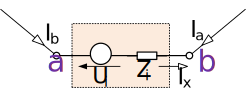
\includegraphics[width=0.7\linewidth]{Biolek_MMUN_thev_dvojpol.pdf}
          \caption[MMUN - Théveninův model dvojpólu]{Začlenění obecného lineárního dvojpólu, 
                   popsaného Théveninovým modelem do obvodu \cite[s.~78]{Biolek}}
          \label{TEO:fig_MMUN_thev_dvojpol}
        \end{figure}
        
        Původní rovnice popisující rovnováhu proudů v uzlu \emph{a} musí být na pravé straně 
        doplněna o proud $I_x$, vytékající ven z uzlu, a v uzlu \emph{b} o proud $I_x$ se záporným 
        znaménkem, protože vtéká dovnitř uzlu \emph{b}. Navíc uzlová napětí $U_a$ a $U_b$ jsou nyní 
        vázána podmínkou
        
        \begin{equation}\label{TEO:eq_MMUN_dvojpol}
          Z_iI_x + U_b = U_i + U_a, \quad\text{neboli}\quad U_i = Z_iI_x + U_b - U_a
        \end{equation}
        Všechny tyto modifikace lze zahrnout do nové soustavy rovnic MMUN:
        
        \begin{figure}[ht!]
          \centering
          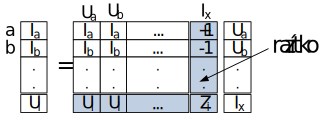
\includegraphics[width=1\linewidth]{Biolek_MMUN_razitko.pdf}
          \caption[MMUN - razítko]{ Razítko v pseudoadmitanční matici \cite[s.~79]{Biolek}}
          \label{TEO:fig_MMUN_razitko}
        \end{figure}
        
        Vektor neznámých uzlových napětí je rozšířen o další neznámou, $I_x$. Počet rovnic je 
        rovněž zvětšen o jedničku, a to o výše uvedenou podmínku mezi uzlovými napětími $U_a$ a 
        $U_b$. Přitom napětí $U_i$ je začleněno do vektoru známých budicích veličin na levé straně. 
        Modifikace rovnic 1. KZ pro uzly \emph{a} a \emph{b} je provedena zápisem $+1$ a $-1$ do 
        sloupce "$I_x$".
        
        Právě provedený zápis je návodem, jak pomocí MMUN analyzovat například obvody obsahující 
        zdroj napětí. Impedance $Z_i$ může být i nulová, pak se bude jednat o ideální zdroj napětí. 
        Při $U_i = 0$ a $I_i = 0$ lze modelovat zkrat mezi uzly a počítat proud, tekoucí tímto 
        zkratem. Toho lze využít například při analýze obvodů s proudem řízenými zdroji. 
        
        V případě, že se v obvodu nachází více prvků bez admitančního popisu, odpovídá každému z 
        nich samostatné razítko. Pseudoadmitanční matice pak nabývá na rozměrech. Metodu budeme 
        blíže konkretizovat na několika příkladech. 
  
        \subsubsection{Pasivní obvody obsahující zdroje napětí a proudu}
          Pomocí MMUN vyřešme zadání z obr. \ref{TEO:fig_MMUN02}. Je hledán proud \(I_x\) vytékající 
          ze zdroje napětí 
          %----------------------------------
          % image: TEO_fce01.tex label: \label{TEO:fig_MMUN02}
            \input{../src/TEO/img/TEO_circ02.tex}  
          %---------------------------------- 
        \subsubsection{Obvody s ideálním operačním zesilovačem ty\-pu VFA}
          Ideální OPAMP, na obr. \ref{TEO:fig_MMUN_ideal_VFA} po vložení do obvodu způsobí 
          ztotožnění uzlových napětí $U_a$ a $U_b$, a modifikaci proudových poměrů v uzlu \emph{c}.
      
          \begin{figure}[ht!]
            \centering
            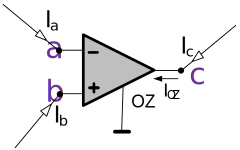
\includegraphics[width=0.6\linewidth]{MMUN_ideal_VFA.pdf}
            \caption[Ideální operační zesilovač typu VFA]{Ideální operační zesilovač typu VFA}
            \label{TEO:fig_MMUN_ideal_VFA}
          \end{figure}
          Ve spodním přídavném řádku je zapsána rovnice
          \begin{equation}\label{TEO:eq_MMUN_VFA}
              0 = 1\cdot U_a - 1\cdot U_b
          \end{equation}
          Výsledek řešení se nezmění, jestliže obě strany této rovnice vynásobíme libovolným 
          nenulovým číslem. Ve spodním řádku tedy může být namísto $[1,-1]$ například $[15,-15]$.
          \begin{figure}[ht!]
            \centering
            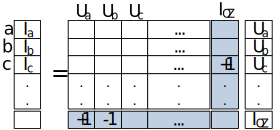
\includegraphics[width=\linewidth]{MMUN_ideal_VFA_matice.pdf}
            \caption[MMUN - pro ideální OPAMP]{MMUN - pro ideální OPAMP typu VFA}
            \label{TEO:fig_MMUN_VFA_matice}
          \end{figure}
          Je-li jeden ze vstupů OZ spojený s referenčním uzlem, neobjeví se příslušné uzlové napětí 
          v rovnicích a proto v posledním řádku bude figurovat jen jedna jednička místo uvedené 
          dvojice. 
          
          Jednička v řádku \emph{c} a sloupci $I_{OZ}$ reprezentuje připočtení proudu $I_{OZ}$ do 
          celkové bilance proudů, vytékající z uzlu \emph{c}.
        
          % --------example: Invertující zesilovač ---------------
          % \label{TEO:ex_InvOpamp01}
            % !TeX spellcheck = cs_CZ
\begin{example}\label{TEO:ex_InvOpamp01}
  Uvažujme invertující zesilovač s ideální operačním zesilovačem typu VFA s naznačenými uzly 
  tak, jak je na obr. \ref{TEO:fig_MMUN_inv_opamp}. Napište rovnice MMUN.
  
   {\centering
    \captionsetup{type=figure}
    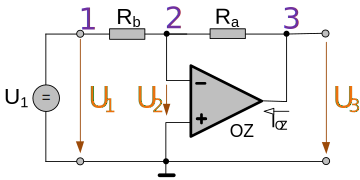
\includegraphics[width=0.7\linewidth]{MMUN_inv_OPAMP.pdf}
    \captionof{figure}{Invertující zesilovač}
    \label{TEO:fig_MMUN_inv_opamp}
    \par}
  
  Rovnice MMUN budou v maticovém zápisu vypadat takto:

    % using \usepackage{array} and command \newcolumntype{C}[1]{>{\centering}m{#1}}!
   {\centering
    \begin{tabular}{|C{0.6cm}|C{1.2cm}|C{0.6cm}|C{0.45cm}|C{0.45cm}|C{.3cm}|c|C{.33cm}|c|}
        \multicolumn{1}{c}{$U_1$}    & \multicolumn{1}{c}{$U_2$}    & \multicolumn{1}{c}{$U_3$}  & 
        \multicolumn{1}{c}{$I_1$}    & \multicolumn{1}{c}{$I_{OZ}$} & \multicolumn{1}{c}{ }      &  
        \multicolumn{1}{c}{x}        & \multicolumn{1}{c}{ }        & \multicolumn{1}{c}{b}       \\
      \cline{1-5}\cline{7-7} \cline{9-9}
      $G_b$  & $-G_b$    &  & -1  &  & \multirow{5}{*}{$\ast$} & $U_1$ & \multirow{5}{*}{=}     & \\
      \cline{1-5} \cline{7-7} \cline{9-9}
      $-G_b$ & $G_a+G_b$ & $-G_a$ &  &   & & $U_2$      &      &                                  \\
      \cline{1-5} \cline{7-7} \cline{9-9}
             & $-G_a$    & $G_a$  &  & 1 & & $U_3$      &      &                                  \\
      \cline{1-5} \cline{7-7} \cline{9-9}
         1   &           &        &  &   & & $I_1$      &      &    $U_{IN}$                      \\
      \cline{1-5} \cline{7-7} \cline{9-9}
             &     1     &        &  &   & & $I_{OZ}$   &      &                                  \\
      \cline{1-5} \cline{7-7} \cline{9-9}
    \end{tabular}
    \par}
  \vspace{1em}
  Předposlední rovnice říká, že uzlové napětí $U_1$ je rovno napětí signálového zdroje $U_{IN}$. 
  Jednička v posledním řádku reprezentuje jednoduchou rovnici $U_2 = 0$. Ačkoliv je obvod poměrně 
  jednoduchý, je pro ruční řešení neefektivní, neboť jsme získali soustavu o 5 rovnic a 5 neznámých.
\end{example}  
          %-------------------------------------------------------

          % --------example: Neinvertující zesilovač -------------
          % \label{TEO:ex_NeinvOpamp01}
            % !TeX spellcheck = cs_CZ
\begin{example}\label{TEO:ex_NeinvOpamp01} 
  Uvažujme neinvertující zesilovač s ideální operačním zesilovačem typu VFA s naznačenými uzly tak, 
  jak je na obr. \ref{TEO:fig_MMUN_neinv_opamp}. Napište rovnice MMUN.

   {\centering
    \captionsetup{type=figure}
    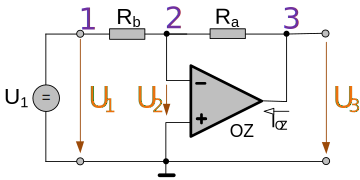
\includegraphics[width=0.7\linewidth]{MMUN_inv_OPAMP.pdf}
    \captionof{figure}{Neinvertující zesilovač}
    \label{TEO:fig_MMUN_neinv_opamp}
    \par}
   % using \usepackage{array} and command \newcolumntype{C}[1]{>{\centering}m{#1}}!
  {\centering
   \begin{tabular}{|C{0.45cm}|C{1.2cm}|C{0.6cm}|C{0.45cm}|C{0.45cm}|C{0.2cm}|c|C{.3cm}|c|}
      \multicolumn{1}{c}{$U_1$} & \multicolumn{1}{c}{$U_2$}   & \multicolumn{1}{c}{$U_3$} & 
      \multicolumn{1}{c}{$I_1$} & \multicolumn{1}{c}{$I_{OZ}$}& \multicolumn{1}{c}{ }     & 
      \multicolumn{1}{c}{x}     & \multicolumn{1}{c}{ }       & \multicolumn{1}{c}{b}     \\ 
      \cline{1-5} \cline{7-7} \cline{9-9}
           &   &   &  -1  &  & \multirow{5}{*}{$\ast$} & $U_1$ & \multirow{5}{*}{=}  &   \\
      \cline{1-5} \cline{7-7} \cline{9-9}
           & $G_a+G_b$ & $-G_a$ &      &   & & $U_2$     &   &                           \\
      \cline{1-5} \cline{7-7} \cline{9-9}
           & $-G_a$    & $G_a$ &       & 1 & & $U_3$     &   &                           \\
      \cline{1-5} \cline{7-7} \cline{9-9}
         1 &           &       &       &   & & $I_1$     &   & $U_{IN}$                  \\
      \cline{1-5} \cline{7-7} \cline{9-9}
           &     1     &       &       &   & & $I_{OZ}$  &   & $U_{IN}$                  \\
      \cline{1-5} \cline{7-7} \cline{9-9}
   \end{tabular}
   \par}
   \vspace{1em}
\end{example}  
          %-------------------------------------------------------
          \newpage
          % --------example: Diferenciální zesilovač -------------
          % \label{TEO:ex_DifOpamp01}
            % !TeX spellcheck = cs_CZ
\begin{example}\label{TEO:ex_DifOpamp01} 
  Uvažujme diferenciální zesilovač s ideální operačním zesilovačem typu VFA s naznačenými 
  uzly tak, jak je na obr. \ref{TEO:fig_MMUN_diff_opamp}. Napište rovnice MMUN.

   {\centering
    \captionsetup{type=figure}
    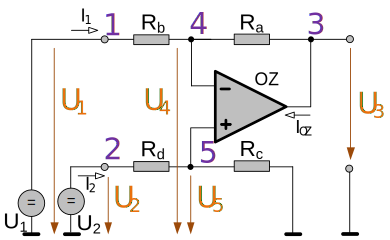
\includegraphics[width=0.7\linewidth]{MMUN_diff_OPAMP.pdf}
    \captionof{figure}{ Diferenciální zesilovač}
    \label{TEO:fig_MMUN_diff_opamp}
    \par}
%  \newpage
%  \begin{widetext}
    % using \usepackage{array} and command \newcolumntype{C}[1]{>{\centering}m{#1}}!
    {\centering
    \begin{tabular}{|C{0.6cm}|C{0.6cm}|C{0.6cm}|C{1.2cm}|C{0.6cm}|C{0.45cm}|C{0.45cm}|C{0.45cm}|}
        \multicolumn{1}{c}{$U_1$}  & \multicolumn{1}{c}{$U_2$}   & \multicolumn{1}{c}{$U_3$}  & 
        \multicolumn{1}{c}{$U_4$}  & \multicolumn{1}{c}{$U_5$}   & \multicolumn{1}{c}{$I_1$}  & 
        \multicolumn{1}{c}{$I_2$}  & \multicolumn{1}{c}{$I_{OZ}$}                      \\
        \hline
        $G_b$  &        &        & $-G_b$    &         & \(-1\) &        &             \\
        \hline
               & $G_d$  &        &           & $-G_d$  &        & \(-1\) &             \\
        \hline
               &        &  $G_a$ & $-G_a$    &         &        &        &             \\
        \hline 
        $-G_b$ &        & $-G_a$ & $G_a+G_b$ &         &        &        &             \\
        \hline
               & $-G_d$ &        & $G_c+G_d$ &         &        &        &             \\
        \hline
               &        &        &  \(-1\)   &  \(1\)  &        &        &             \\
        \hline
         1     &        &        &           &         &        &        &             \\
        \hline   
               & \(1\)  &        &           &         &        &        &             \\
        \hline    
    \end{tabular}
    \par}
%    \vspace*{0.5cm}
%  \end{widetext}
\end{example}  
          %-------------------------------------------------------

  \section{Analýza pomocí numerického simulátoru}
    \subsection{Analýza „DC“ neboli stejnosměrná analýza}
    \subsection{Rozšiřující typy analýz}
      \subsubsection{Citlivostní analýza („Sensitivity“)}
        Je počítána \emph{stejnosměrná citlivost} jedné nebo více veličin, vyjádřené vzorcem nebo 
        vzorci, na jednu nebo více vstupních proměnných.

          % --example: Citlivostní analýza napěťový děliče -------
          % \label{TEO:ex_CitDiveder01}
            % !TeX spellcheck = cs_CZ
\begin{example}\label{TEO:ex_CitDiveder01}
  V elektronických soustavách se největších přesností dosahuje u rezistorů, kde je standardně 
  zaručována chyba menší než 1\%, u přesných 0.1\% a u velmi přesných 0.01\%.

   {\centering
    \captionsetup{type=figure}
    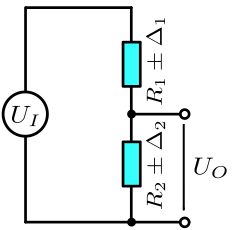
\includegraphics[width=0.4\linewidth]{voltage_divider.pdf}
    \captionof{figure}{ }
    \label{TEO:fig_voltage_divider}
    \par}

  Bude nás zajímat jaký vliv má tolerance rezistorů na výsledný poměr výstupního ku vstupnímu 
  napětí a také, zda-li při různě zvoleném poměru těchto rezistorů se bude měnit velikost chyby, 
  ačkoliv budou mít stejnou přesnost. Intuitivně předpokládáme, že  nejnepříznivější situace  
  nastane, když hodnoty použitých rezistorů padnou na opačné strany tolerančních pásem, jenž 
  reprezentuje $\Delta_1$ a $\Delta_2$ tj. $R_2 - \Delta_2R_2$ a $R_1 + \Delta_1R_1$ nebo $R_2 + 
  \Delta_2R_2$ a $R_1 - \Delta_1R_1$. V obou případech bude chyba stejná, proto si vybereme 
  například první případ a zapíšeme (rov. \ref{TEO:eq_divider_1}).
  \begin{equation}\label{TEO:eq_divider_1}
    \frac{U_o}{U_i} = \frac{R_2-\Delta_2 R_2}{R_1+\Delta_1 R_1+R_2-\Delta_2 R_2}
  \end{equation}
  a po úpravě
  \begin{equation*}
     \frac{U_o}{U_i} = \frac{(1-\Delta_2) R_2}{(1+\Delta_1) R_1+(1-\Delta_2) R_2}
  \end{equation*}
  Polynom ve jmenovateli rozvineme do následující podoby
  \begin{align*}
     [(1+\Delta_1) &+ (1-\Delta_2)](R_1+R_2)                \\
                   &= (1+\Delta_1)R_1 + (1-\Delta_2)R_2     \\
                   &+ (1+\Delta_1)R_2 + (1-\Delta_2)R_1     \\
   (1+\Delta_1)R_1 &+ (1-\Delta_2)R_2                       \\
                   &= [(1+\Delta_1)+(1-\Delta_2)](R_1+R_2)  \\
                   &- (1+\Delta_1)R_2 - (1-\Delta_2)R_1 
  \end{align*}
  a získáme %Further simplification of the denominator yields
  {\footnotesize
  \begin{equation*}
      \dfrac{U_o}{U_i}\ =
        \dfrac{(1-\Delta_2) R_2}{[(1+\Delta_1) + (1-\Delta_2)](R_1+R_2) - 
        [(1+\Delta_1) R_2\ +\ (1-\Delta_2) R_1] }
  \end{equation*}
  } %
  Nyní vydělíme jmenovatel i čitatel $(R_1 + R_2)$ a dostaneme 
  % Next divide both numerator and denominator by R1 + R2
  \begin{equation*}\label{TEO:eq_divider_2}
    \frac{U_o}{U_i}\ =\dfrac{\dfrac{(1-\Delta_2) R_2}{R_1+R2}}{[(1+\Delta_1)+(1-\Delta_2)] - 
    \dfrac{[(1+\Delta_1) R_2\ +\ (1-\Delta_2) R_1]}{R_1+R_2} }
  \end{equation*}
  Standardně rezistory volíme se stejnou tolerancí, tedy $\Delta_1 = \Delta_2 = \Delta$ a získáme 
  výslednou rovnici pro poměr $\frac{U_o}{U_i}$ 
  % Based on the assumption that both $\Delta1 = \Delta2 = \Delta$ then it should be possible to  
  % further simplify the expression for Vo/Vi:
  \begin{equation}
     \dfrac{U_o}{U_i} = \dfrac{\dfrac{(1-\Delta) R_2}{R_1+R_2}}{[(1+\Delta)+(1-\Delta)] - 
     \dfrac{[(1+\Delta)R_2 + (1-\Delta) R_1]}{R_1+R_2} }
  \end{equation}

  Řekněme například, že pro návrh děliče máme k dispozici rezistory s tolerancí 1\% a vstupní 
  napětí je 1 V. Obvod, ve kterém je dělič použit, umožňuje volit různé poměry, ale jejich součet 
  je konstantní. Na otázku jaký poměr zvolit, abychom při dané toleranci rezistorů dostali 
  výstupní napětí s největší přesností odpovídá následující tabulka.
  \vspace{1em}
  
  {\centering
   \setlength{\tabcolsep}{5pt}
   \begin{tabular}{|c|c|c|c|}
      \hline
        $R_1$                 & $1 k\Omega$  & $10 k\Omega$     & $19 k\Omega$   \\
      \hline
        $R_2$                 & $19 k\Omega$ & $10 k\Omega$     & $1 k\Omega$    \\
      \hline
        $U_{out}$             & 0,950        & 0,500            & 0,050          \\
      \hline
        $U_{out}^*$           & 0,949        & 0,495            & 0,049          \\
      \hline
        $\varepsilon_r [\%]$  & 0,101        & 1,000            & 1,883          \\
      \hline
   \end{tabular}
  \par}
  \vspace{1em}

  % Let's compare this answer to the formula I gave in a previous post using differentials. The  
  % relevant differential is
  % \begin{equation}\label{TEO:eq_divider_8}
  %   dV_0 = ( \frac{V}{R_1+R_2} - \alpha ) dR_1 - \alpha dR_2 + \frac{R_1}{R_1+R_2} dV
  % \end{equation}
  % where
  % \begin{equation}\label{TEO:eq_divider_9}
  %   \alpha = \frac{R_1 V}{(R_1+R_2)^2}
  % \end{equation}
\end{example}  
    
          %-------------------------------------------------------
} % \tikzset

%---------------------------------------------------------------------------------------------------
\printbibliography[title={Seznam literatury}, heading=subbibliography]
\addcontentsline{toc}{section}{Seznam literatury}
%========== Kapitola: Přechodné děje ==============================================================
  \input{../src/TEO/chap/teo1ch05.tex}
%========== Kapitola: Obvody v harmonickém ustáleném stavu ========================================
  \input{../src/TEO/chap/teo1ch07.tex}
%========== Kapitola: Obvody s rozprostřenými parametry ===========================================
  % !TeX spellcheck = cs_CZ
%file: teo1ch03.tex
%===========Kapitola: Obvody s rozprostřenými parametry====================================
\setchaptertoc
\chapter{Obvody s rozprostřenými parametry}\label{teo:IchapIX}

%~~~~~~~~~~~~~~~~~~~~~~~~~~~~~~~~~~~~~~~~~~~~~~~~~~~~~~~~~~~~~~~~~~~~~~~~~~~~~~~~~~~~~~~~~~~~~~~~~~  
%=============== Seznam literatury ================================================================
  \printbibliography[title={Seznam literatury}, heading=bibliography]
}  % DEBUG was off
%--------------------------------------------------------------------------------------------------
%                                       /$$$$$$$$  /$$$$$$ 
%                                       | $$_____/ /$$__  $$
%                                       | $$      | $$  \__/
%                                       | $$$$$   |  $$$$$$ 
%                                       | $$__/    \____  $$
%                                       | $$       /$$  \ $$
%                                       | $$$$$$$$|  $$$$$$/
%                                       |________/ \______/                     
%--------------------------------------------------------------------------------------------------
\ifthenelse{ \equal{\DebugMode}{true} }{ % Debug mode ON
  % !TeX program = lualatex
% !TeX root = luaking.tex
% !TeX encoding = UTF-8
% !TeX spellcheck = cs_CZ
%=================== Kapitola: Bipolární tranzistory ==============================================
\setchaptertoc
\chapter{Bipolární tranzistory}\label{es:IchapV}
  \section{Všeobecné poznatky}\label{es:IchapVsecI}
    Tranzistor je polovodičový prvek určeny na zesilovaní nebo generovaní elektrických signálu,
    jedná se tedy o \emph{aktivní} součástku.

    Podle činnosti rozdělujeme tranzistory: 
    \begin{itemize}[noitemsep]
      \item s injekcí, které využívají majoritní i minoritní nosiče (bipolární),
      \item řízené polem, které využívají pouze majoritní nosiče náboje (unipolární).
    \end{itemize}
     
    Bipolámí tranzistory představují aktivní polovodičové prvky. Jsou tvořeny dvěma přechody PN,
    tzn. třemi vrstvami z rozdílně dotovaného polovodičového materiálu. Podle pořadí vrstev
    rozlišujeme dvě skupiny bipolárních tranzistorů, a to tranzistory \textsc{NPN} a tranzistory
    \textsc{PNP}. Obě uspořádání tranzistorů jsou znázorněna na obr. \ref{teo:fig053}, kde je
    zobrazeno jak pořadí vrstev, tak příslušná schematická značka.

    \begin{figure}[ht!]
      \centering  
      \subcaptionbox{\textsc{PNP}\label{teo:fig053a}}{\luafigure[0.3]{teo_fig053a.pdf}} \hspace{1em}
      \subcaptionbox{\textsc{NPN}\label{teo:fig053b}}{\luafigure[0.3]{teo_fig053b.pdf}} \\
      \subcaptionbox{\label{teo:fig053c}}{\luafigure[0.3]{teo_fig053c.pdf}}             \hspace{1em}
      \subcaptionbox{\label{teo:fig053d}}{\luafigure[0.3]{teo_fig053d.pdf}}                   
      \caption{Pořadí vrstev polovodiče a schematická značka bipolárních NPN a PNP 
      tranzistorů (\cite[s.~112]{Frohn2006})}
      \label{teo:fig053}
    \end{figure}
    
    Označení \uv{tranzistor} je uměle vytvořené slovo z anglických slov \textbf{tran}sfer = přenášet
    a re\textbf{zistor} = odpor. Označení \uv{bipolámí} (bi = dva) má poukázat na skutečnost, že je
    hlavní proud určen dvěma rozdílnými druhy nositelů náboje. Ve všeobecném povědomí se však pro
    bipolární tranzistor ustálil zjednodušený pojem tranzistor. Na rozdíl od bipolárních tranzistorů
    teče u unipolárních tranzistorů (unum = jeden) hlavní proud pouze jedinou oblastí a z toho
    vyplývá, že je určen pouze jediným typem nositele náboje podle toho, jakým způsobem byl dotován
    polovodičový materiál. Unipolární tranzistory často označujeme jako tranzistory řízené
    elektrickým polem. Jejich princip bude uveden v kapitole \ref{es:IchapVI}.
    
    Pro uživatele má velký význam znalost vlastností a chování jednotlivých typů tranzistorů. Proto
    výrobci ke každému typu tranzistoru vydávají katalogové listy, které obsahují charakteristické
    hodnoty, charakteristiky a mezní hodnoty (obdobně jako u diod).
    
    Protože tranzistor představuje dvojbran, jenž má dvě vstupní a dvě výstupní elektrody, je počet
    charakteristických hodnot a charakteristik podstatně větší než u polovodičových diod. Některé
    důležité parametry a charakteristiky budou blíže objasněny v následujících odstavcích.
    
    Bipolární tranzistory využívají jako výchozího materiálu nejčastěji křemíku, pro vysoké kmitočty
    se používají tranzistory ze sloučenin typu \(A^{III}B^{V}\).
    
    Tranzistory můžeme rozdělovat podle mnoha hledisek. Z hlediska konstrukce je zásadní rozdělení
    na tranzistory pro malé signály (nízkého výkonu) a výkonové tranzistory. Takovéto rozdělení
    podle konstrukce je uvedeno na obr. \ref{teo:fig073}.
    
    Tranzistory nízkého výkonu se převážně používají pro zesilování malých střídavých signálů.
    Tranzistory mají v tomto případě pevně nastavený klidový pracovní bod a přiváděné signálové
    napětí je malé, tzn. že nesmějí být příliš vybuzeny. Další oblastí použití tranzistorů nízkého
    výkonu jsou elektronické spínače, které jsou buzeny v celém možném rozsahu charakteristik.
    
    Výkonové tranzistory jsou dimenzovány na velké proudy a velká napětí. Mají proto relativně větší
    pouzdra, díky nimž je možné rychleji odvádět větší množství vznikajícího tepla z krystalu
    polovodiče. Výkonové tranzistory nalézají uplatnění v zesilovačích velkých signálů, tj.
    výkonových a koncových stupních nebo zastávají funkci elektronických spínačů.

    \begin{mdframed}[style=mdnote]
      \small
      Krátce po skončení války v roce 1945, Bellovy laboratoře vytvořily skupinu pro výzkum fyziky
      pevných látek, pod vedením \textsc{Shockleyho}. Jejich cílem bylo najít alternativu ke křehkým
      elektronkovým zesilovačům. Jejich první pokusy byly založeny na Shockleyově myšlence, že
      vnější elektrické pole na polovodiči ovlivní jeho vodivost. Jejich experimenty však záhadně
      selhávaly.

      Skupina začala studovat atomové struktury, které se na povrchu a uvnitř látek liší. Hledané
      výsledky se začaly dostavovat v okamžiku, když začali obklopovat body dotyku mezi polovodičem
      a přívodními vodiči elektrolytem. \textsc{Hilbert Moore} postavil okruh, který jim dovolil
      snadno měnit frekvenci vstupního signálu a navrhl, aby používali glykol boritan, viskózní
      chemikálii, která se nevypařovala. Nakonec získali důkaz schopnosti zesílení signálu, když
      fyzik \textsc{Gerald Pearson}, podle návrhu Shockleyho, uvedl napětí na kapičku glykol
      boritanu umístěnou přes \textsc{P-N} přechod. V prosinci 1947 Bardeen a Brattain – pracovali
      bez Shockleyho – uspěli ve stvoření hrotového tranzistoru, který zesiloval signál.

      Další měsíc začali patentoví zástupci Bellových laboratoří pracovat na patentových
      přihláškách. Brzo objevili, že Shockleyho vliv elektrického pole na polovodič byl předpovídán
      a patentován v roce 1930 \textsc{Juliem Lilienfeldem}, který si svůj \textsc{MESFET}
      patentoval v Kanadě již v 22. října 1925. Přesto byly podány celkem čtyři žádosti o patent. Na
      žádné z těchto přihlášek se však nevyskytovalo Shockleyovo jméno. To Shockleyho rozzlobilo,
      protože práce byla založena na jeho nápadu s účinkem elektrického pole. 
      
      Ve stejnou dobu tiše pokračoval ve vlastní práci na stavbě různých druhů tranzistoru
      založených na spojení místo bodového dotyku. Předpokládal, že tento typ tranzistoru bude více
      komerčně úspěšný. Shockley pracoval na \emph{teorii elektronů a děr v polovodičích}, která
      byla nakonec vydána jako 558 stránková monografie v roce 1950. V té Shockley vypracoval
      rozhodující myšlenky týkající se pohybu elektronů a děr a diferenciální rovnici, kterou se
      řídí tok elektronů v pevných krystalech.

      Shockleyho tato práce vedla k myšlence \emph{sendvičového tranzistoru} a ke vzniku klasického
      tranzistoru. Jeho objev byl oznámen 4. června 1951 a Shockley obdržel 25. září 1951 za jeho
      objev patent. Pro výrobu tohoto tranzistoru byla vyvinuta difúzní metoda a tento tranzistor
      brzy zastínil tranzistor s bodovými kontakty. Shockley pokračoval jako vedoucí skupiny v
      Bellových laboratořích ještě dva roky.

      {\centering
        \captionsetup{type=figure}
        \luafigure[1]{teo_fig071.png}
        \captionof{figure}{\textsc{John Bardeen}, \textsc{William Shockley} a \textsc{Walter Brattain} 
          v Bell Labs, 1948. (\cite[s.~6]{KolkaBiolek2011})
        \label{teo:fig071}}
      \par}

      V roce 1951 byl zvolen členem National Academy of Sciences (NAS). Za svůj objev tranzistoru
      získal mnoho cen. Bellovy laboratoře však představovaly všechny tři vynálezce (Shockleyho,
      Bardeena a Brattaina) jako tým. To vedlo k rozkolu a Shockley později blokoval práci Bardeena
      a Brattaina na klasickém tranzistoru.

      Shockley nakonec začal řídit svoji vlastní společnost, v níž se pokoušel vytvořit nové a
      technicky obtížné zařízení (původně nazvané čtyřvrstvá dioda a nyní známé jako tyristor).
      Projekt se ale rozvíjel velmi pomalu. 

      V roce 1956 Shockley získal, spolu s Bardeenem a Brattainem, Nobelovu cenu za fyziku. Ve své
      Nobelovské přednášce plně ocenil Brattaina a Bardeena jako vynálezce tranzistoru s bodovými
      kontakty.
    \end{mdframed}
    
    Pro lepší orientaci ve velkém množství vyráběných typů tranzistorů bylo zavedeno označovací
    schéma. Evropští výrobci používají hlavně značení \uv{Pro-Electron\footnote{Pro Electron nebo
    EECA je evropský typový a registrační systém pro aktivní komponenty (jako jsou polovodiče,
    displeje z tekutých krystalů, senzorová zařízení, elektronky a katodové trubice). Společnost Pro
    Electron byla založena v roce 1966 v belgickém Bruselu. V roce 1983 byla sloučena s Evropskou
    asociací výrobců elektronických součástek (EECA) a od té doby působí jako agentura EECA.}},
    které využívá kombinace písmen a číslic.

    \luagraphic[1]{teo_fig079.jpg}{Pohled na čip \textsc{MJ1000} v TO3 pouzdře. Čip obsahuje dva 
      tranzistory v Darlingtonovo zapojení. První, méně výkonný tranzistor se zesílením cca 100 
      budí druhý výkonový tranzistor se zesílením cca 10. Výsledný zesilovací činitel je dán 
      přibližně vynásobením zesilovacích činitelů obou tranzistorů (cca 1000).}{teo:fig079}

    Aby mohl tranzistor řádně pracovat, musí mít potřebné napětí nejen mezi kolektorem a emitorem,
    ale také dostatečně velké napětí mezi bází a emitorem. Velkou roli přitom hraje teplotní
    stabilizace klidového pracovního bodu. Je potřebná z toho důvodu, že při stoupající teplotě
    okolí narůstají též proudy, které tranzistorem protékají. Následkem zvyšování teploty se krystal
    ohřívá a roste tak jeho vodivost, čímž se příslušné proudy zvětšují. Tímto způsobem stoupá
    ztrátový výkon, tranzistor se proto více ohřívá atd. Na konci tohoto koloběhu je tepelná
    destrukce tranzistoru, který se tak stává nepoužitelným.

    \begin{figure*}
      \centering
      \luafigure[1]{teo_fig073.png}
      \caption{Druhy bipolárních tranzistorů podle konstrukce. (\cite[s.~115]{Frohn2006})}
      \label{teo:fig073}
    \end{figure*}

    Tranzistory mohou pracovat ve třech různých základních zapojeních - se společným emitorem
    (\textsc{SE}), se společným kolektorem (\textsc{SC}) a se společnou bází (\textsc{SB}). Zapojení
    je pojmenováno podle toho, která z elektrod je společná vstupu a výstupu zesilovacího stupně pro
    zesilování střídavých napětí, tj. která představuje společný pól signálového napětí na vstupu a
    na výstupu daného stupně. Každé z těchto základních zapojení má své přednosti a nedostatky.
    Nejčastěji se používá zapojení \textsc{SE}. Zapojení \textsc{SC} se používá jako měnič impedance
    (velká vstupní a malá výstupní impedance). Zapojení \textsc{SB} má svůj význam hlavně ve
    vysokofrekvenční technice, jinak představuje také měnič impedance, avšak s přesně opačným
    účinkem než předchozí zapojení (malá vstupní a velká výstupní impedance).

    Při praktickém využití musejí být tranzistory, a to ať se jedná o jakékoliv zapojení, doplněny
    dalšími součástkami. Zapojení těchto součástek (rezistorů a kondenzátorů) závisí na tom, jakou
    úlohu má zapojení s tranzistorem plnit. Musíme rozlišit, zda má tranzistor pracovat ve
    stejnosměrném zesilovači, v zesilovači střídavých napětí, ve výkonovém zesilovači nebo zda má
    mít funkci spínače.

    Stejnosměrné zesilovače se používají všude tam, kde je zapotřebí zesilovat stejnosměrná napětí a
    změny napětí od velmi malých až k vysokým frekvencím. Typickým představitelem je např. zesilovač
    Y osciloskopu. Aby stejnosměrné zesilovače mohly řádně plnit svou funkci, nesmějí obsahovat
    žádné součástky, které by ovlivňovaly jejich zesílení na různých frekvencích a neumožňovaly
    galvanickou vazbu (např. kondenzátory).

    Střídavé zesilovače mohou naproti tomu zesilovat střídavá napětí o frekvenci několika \si{\Hz}
    až do několika \si{\GHz} (podle typu tranzistoru a dimenzování zapojení), avšak nemusejí
    zesilovat stejnosměrná napětí. Důležitými prvky v těchto zesilovačích jsou kondenzátory.

    Výkonové zesilovače mají spotřebiči odevzdat pokud možno co největší signálový výkon. Spotřebič
    může být představován např. reproduktorem (nízkofrekvenční výkonový zesilovač), vysílací anténou
    (vysokofrekvenční výkonový zesilovač) nebo motorem (aplikace výkonového zesilovače v regulační
    technice). Na spínače jsou kladeny zcela jiné požadavky než na stejnosměrné nebo střídavé
    zesilovače. Spínače mají co nejrychleji přecházet ze stavu \uv{zapnuto} do stavu \uv{vypnuto} a
    naopak. V tomto případě hrají velkou roli parazitní kapacity tranzistorů.


  \section{Základní princip}\label{es:IchapVsecII}
    \subsection{Princip funkce NPN a PNP tranzistorů}\label{es:IchapVsecIIssecI}
      První tranzistory byly vyráběny legováním. Tato technologie byla převzata z výroby diod. Aby
      byly vyrobeny dva přechody, byly na obě strany dotovaného základního materiálu umístěny
      pilulky cizích prvků - donorů nebo akceptorů {obr. \ref{teo:fig072}. Při výrobním procesu pak
      cizí atomy z obou stran difundovaly do výchozího materiálu. Střední vrstva byla přitom velmi
      tenká a měla výrazně menší počet volných nositelů náboje než obě vnější vrstvy. Podle
      použitých výchozích materiálů a cizích prvků vznikl tranzistor NPN nebo PNP.

      \luagraphic[0.8]{teo_fig072.png}{Výroba tranzistoru NPN legováním.
        (\cite[s.~115]{Frohn2006})}{teo:fig072}
      
      Aby tranzistor fungoval, musí být mezi bázi a emitor připojen zdroj napětí tak, aby byl spodní
      přechod PN polarizován v propustném směru. Tranzistor NPN má proto bázi kladnější než emitor,
      tranzistor PNP má bázi zápornější než emitor. Napětí mezi bází a emitorem křemíkových
      tranzistorů má velikost \(U_{BE} \approx \SI{0.7}{\V}\), tj. stejné, jako je difuzní napětí
      křemíkových diod. Na obr. \ref{teo:fig074} a \ref{teo:fig075} zakreslené proudy vyznačují směr
      toku elektronů.

      \luagraphic[1]{teo_fig074.png}{Znázornění tranzistoru NPN. \(\longrightarrow\) udáva směr 
        toku elektronů). (\cite[s.~116]{Frohn2006})}{teo:fig074}
      
      Horní přechod PN pracuje v závěrném směru. Zdroje napětí jsou z tohoto důvodu zapojeny tak,
      aby byl kolektor u NPN tranzistoru kladnější než emitor, u PNP tranzistoru naopak zápornější
      než emitor.

      Vlivem připojených napětí bude spodní přechod PN zapojen v propustném směru a horní přechod PN
      v závěrném směru. Ve střední a horní oblasti se vytvoří závěrná vrstva. Ta se rozprostírá
      téměř po celé šířce střední oblasti, která je velmi tenká a obsahuje pouze malý počet nositelů
      náboje.        

      \luagraphic[1]{teo_fig075.png}{Znázornění tranzistoru PNP.  \(\longrightarrow\) udáva směr 
        toku elektronů). (\cite[s.~116]{Frohn2006})}{teo:fig075}
      
      Protože je spodní přechod PN zapojen v propustném směru, zaplavují nositelé náboje z emitoru
      závěrnou vrstvu ve střední oblasti. Tím se tato závěrná vrstva zmenší a její odpor klesne. Tím
      mohou nositelé náboje z emitoru projít zmenšenou závěrnou vrstvou do kolektorové oblasti a
      odtud odtéct k baterii (ke zdroji).

      Jelikož nositelé náboje pocházejí ze spodní oblasti, nazývá se tato oblast emitor. Střední
      oblast představuje výchozí bod pro oba přechody PN a nazývá se proto bází. Horní oblast
      shromažďuje všechny nositele náboje, které neodtekly bází a nese označení kolektor.

      \luagraphic[1]{teo_fig076.png}{Provozní napětí a proudy tranzistoru NPN. 
        (\cite[s.~117]{Frohn2006})}{teo:fig076}
      
      Proud \(l_B\), který odtéká vývodem báze, je podstatně menší než kolektorový proud \(l_C\),
      jenž protéká zmenšenou závěrnou vrstvou. Např. při napětí \(U_{BE} \approx \SI{0.7}{\V}\)
      protéká bází proud \(I_B = \SI{1}{\mA}\) a kolektorem proud \(I_C \approx \SI{100}{\mA}\).
      Jestliže nyní nepatrné zvětšíme \(U_{BE}\), vzroste proud báze např. na \(I_B = \SI{2}{\mA}\),
      čímž k závěrné vrstvě doputuje více nositelů náboje z emitoru. Tím se závěrná vrstva ještě
      více zmenší a kolektorový proud vzroste např. na \(I_C \approx \SI{200}{\mA}\). Naopak při
      zmenšení napětí \(U_{BE}\) a tím též proudu \(l_B\) se odpor závěrné vrstvy zvětší a
      kolektorový proud \(I_C\) klesne. Zjišťujeme, že proud báze \(l_B\) a proud kolektoru \(l_C\)
      tranzistoru se v širokém rozmezí mění proporcionálně. U tranzistoru je tak možné malým proudem
      báze \(l_B\), jenž představuje vstupní proud, řídit podstatně větší kolektorový proud \(l_C\),
      který je výstupním proudem. Tato souvislost se udává formou \emph{proudového zesílení
      nakrátko} \(\beta\).

      \begin{equation*}
        \beta = \dfrac{\Delta I_C}{\Delta I_B} \qquad \text{při (\(U_{CE} = 0\))}
      \end{equation*}
        
      \luagraphic[1]{teo_fig077.png}{Provozní napětí a proudy tranzistoru PNP. 
        (\cite[s.~117]{Frohn2006})}{teo:fig077}
      
      Tranzistory NPN a PNP se navzájem principiálně odlišují pořadím vrstev. Proto se odlišují též
      polaritou napětí \(U_{BE}\) a \(U_{CE}\). Obr. \ref {teo:fig076} a \ref {teo:fig077}
      vysvětluje souvislosti, které již byly naznačeny na obr. \ref{teo:fig074} a \ref{teo:fig075},
      tentokrát jsou ale použity schematické značky obou typů tranzistorů. Údaj napětí \(U_BE\) a
      \(U_{CE}\) je tvořen tak, že poslední písmeno udává vztažnou elektrodu, zde tedy emitor E. Při
      určování směru toku proudu vycházíme z technické orientace, jež je obvyklá (proud teče obvodem
      směrem od kladného k zápornému pólu zdroje). Všechny proudy, které tečou do tranzistoru, jsou
      kladné, vytékající proudy mají záporné znaménko.

      Aby byl tranzistor schopen činnosti, musí být vždy přechod báze-emitor v propustném směru a
      přechod báze-kolektor v závěrném směru.

      Na obr. \ref{teo:fig078a} je mezi vývod kolektoru a baterii zařazen ještě kolektorový rezistor
      \(R_C\), který plní funkci pracovního odporu. Ten omezuje proudové zesílení tranzistoru a
      přeměňuje je v napěťové zesílení. Tranzistor a kolektorový rezistor v tomto případě tvoří
      napěťový dělič pro napájecí napětí \(U_{CC} = \SI{+10}{\V}\). Při \(I_C = \SI{5}{\mA}\) a
      \(R_C = \SI{1}{\kohm}\) vzniká na kolektorovém rezistoru úbytek napětí
      \begin{equation*}
        U_{RC} = \SI{5e-3}{\mA}\cdot\SI{1}{\kohm} = \SI{5}{\V}
      \end{equation*}

      \luagraphic[1]{teo_fig078a.jpg}{apěťové zesílení tranzistoru NPN. 
        (\cite[s.~117]{Frohn2006})}{teo:fig078a}

      Napětí kolektor-emitor tranzistoru, které představuje výstupní napětí, bude 
      \begin{equation*}
        U_{CE} = U_{CC} - U_{RC} = \SI{10}{\V} - \SI{5}{\V} = \SI{5}{\V}
      \end{equation*}
      Jestliže se napětí \(U_{BE}\) vlivem střídavého napětí z připojeného generátoru v daný okamžik
      zvětší např. na \(U_{BE} = \SI{0.71}{\V}\), vzroste proud báze, který způsobí zvětšení
      kolektorového proudu, který, dejme tomu, vzroste z \(I_C = \SI{5}{\mA}\) na \(I_C =
      \SI{6.5}{\mA}\). Tento zvětšený kolektorový proud vyvolá na kolektorovém rezistoru zvětšený
      úbytek napětí
      \begin{equation*}
        U_{RC} = I_C\cdot R_C = \SI{6.5}{\mA}\cdot\SI{1}{\kohm} = \SI{6.5}{\V}
      \end{equation*}
      Tím napětí \(U_{CE}\) klesne na hodnotu \(U_{CE} = \SI{3.5}{\V}\). Při záporné půlvlně napětí
      generátoru se proud báze \(I_B\) zmenší, čímž se zmenši i proud kolektoru \(l_C\) a tím i
      úbytek napětí na kolektorovém rezistoru \(U_{RC}\). Důsledkem tohoto děje je zvětšení
      \(l_{CE}\) tranzistoru. Příslušné časové průběhy na obr. \ref{teo:fig078}. Generátor,
      připojený na bázi tranzistoru, způsobí změnu proudu báze \(\Delta I_B = \SI{20}{\micro\A}\),
      která vyvolá změnu kolektorového proudu \(\Delta I_C = \SI{3}{\mA}\).

      \begin{figure}[ht!]  %\ref{teo:fig078} 
        \centering
        \subcaptionbox{\(U_{BE}(t)\)\label{teo:fig078b}}{\luafigure[0.9]{teo_fig078b.jpg}}  \\                                                       
        \subcaptionbox{\(I_{B}(t)\) \label{teo:fig078c}}{\luafigure[0.9]{teo_fig078c.jpg}}  \\                  
        \subcaptionbox{\(I_{C}(t)\) \label{teo:fig078d}}{\luafigure[0.9]{teo_fig078d.jpg}}  \\                 
        \subcaptionbox{\(U_{RC}(t)\)\label{teo:fig078e}}{\luafigure[0.9]{teo_fig078e.jpg}}  \\                  
        \subcaptionbox{\(U_{CE}(t)\)\label{teo:fig078f}}{\luafigure[0.9]{teo_fig078f.jpg}}  \\                   
        \caption{Napěťové zesílení tranzistoru zapojeného podle obr. \ref{teo:fig078a} 
          (\cite[s.~118]{Frohn2006})}
        \label{teo:fig078}
      \end{figure}

      Odtud pro uvedený případ zjistíme \emph{proudové zesílení} tranzistoru
      \begin{equation*}
        \beta = \dfrac{\Delta I_C}{\Delta I_B} = \dfrac{\num{3e-3}}{\num{20e-6}} = 150
      \end{equation*}
      \emph{Napěťové zesílení} \(A_u\) zapojení s tranzistorem je definováno podobně jako proudové
      zesílení.
      \begin{equation*}
        A_u = \dfrac{\Delta U_{out}}{\Delta U_{in}} = \dfrac{\Delta U_{CE}}{\Delta U_{BE}}
      \end{equation*}
      Napěťové zesílení závisí kromě proudového zesílení také na velikosti kolektorového rezistoru
      \(R_C\). V příkladu způsobí vstupní střídavé napětí \(\Delta U_{BE} = \SI{-0.02}{\V}\) změnu
      výstupního střídavého napětí \(U_{CE} = \SI{-3}{\V}\). V tomto případě je tedy napěťové
      zesílení
      \begin{equation*}
        A_u = \dfrac{\Delta U_{CE}}{\Delta U_{BE}} = \dfrac{\num{-3}}{\num{0.02}} = -150
      \end{equation*}
      Pomocí kolektorového rezistoru \(R_{C}\) se změnilo proudové zesílení na napěťové zesílení
      tranzistoru. Znaménko \uv{-} naznačuje, že kladné půlvlně vstupního napětí odpovídá záporná
      půlvlna výstupního napětí.

  \section{Základní zapojení tranzistoru}\label{es:IchapVsecIII}
%---------------------------------------------------------------------------------------------------
}{ % DEBUG was off
\LuaPartBckgrnd{titleBG_fractal1.png}
\LuaPartTitle{ES I}{Elektronické součástky}{ESI}
\parttoc
%========== Kapitola: Pasivni součástky ==========================================================
  % !TeX spellcheck = cs_CZ
% file: kap_optocoupler.tex
%{\tikzset{external/prefix={tikz/TEO/}}
% \tikzset{external/figure name/.add={ch12_}{}}
%=================== Kapitola: Optoelektronika =====================================================
\setchaptertoc
\chapter{Pasivní elektronické součáskty}\label{teo:IchapXII}


  \section{Teplotní závislost pasivních prvků}\label{teo:IchapXIIsecI}
    
    \begin{example}\label{teo:exam001}
      Uvažujeme žárovku \qty{100}{\watt}, \qty{230}{\volt} s wolframovým vláknem s teplotním 
      součinitelem odporu \(\alpha = \qty{4.8e-3}{\per\kelvin}\).  Problematické je určení provozní 
      teploty vlákna. Vzhledem k tomu, že wolfram taje při teplotě \qty{3387}{\degreeCelsius} a 
      vlákno svítí bílým žárem, odhadneme teplotu na \qty{2500}{\degreeCelsius}. Ze vztahu \(P = 
      U^2/R\) určíme odpor vlákna: \(R = 230^2/100 = \qty{529}{\ohm}\). Odpor při pokojové teplotě 
      bude: 
      \(R_{20}=529/(1+\num{4.8e-3}\cdot2480) = \qty{41}{\ohm}\). 
      \begin{figure}[ht!]  %\ref{teo:fig018}
        \centering
        \includegraphics[width=0.3\linewidth]{teo_fig018.jpg}
        \caption{Žárovka jednoduchým způsobem přeměňuje elektrickou energii na světlo, zahříváním 
        tenkého wolframového vodiče průchodem elektrického proudu.}
        \label{teo:fig018}
      \end{figure}
      Podle tohoto přibližného výpočtu se zmenší odpor vlákna  téměř třináctkrát a odpovídajícím 
      způsobem vzrůstá i nárazový proud při zapnutí obvodu oproti ustálenému stavu. Z tohoto 
      pohledu měly původní Edisonovy uhlíkové žárovky lepší vlastnosti, protože teplotní součinitel 
      uhlíku je záporný (\cite[s.~84]{Lanicek1998}).
    \end{example}
%} % tikzset
%---------------------------------------------------------------------------------------------------
%========== Kapitola: Bipolární transzistory =====================================================
  % !TeX program = lualatex
% !TeX root = luaking.tex
% !TeX encoding = UTF-8
% !TeX spellcheck = cs_CZ
%=================== Kapitola: Bipolární tranzistory ==============================================
\setchaptertoc
\chapter{Bipolární tranzistory}\label{es:IchapV}
  \section{Všeobecné poznatky}\label{es:IchapVsecI}
    Tranzistor je polovodičový prvek určeny na zesilovaní nebo generovaní elektrických signálu,
    jedná se tedy o \emph{aktivní} součástku.

    Podle činnosti rozdělujeme tranzistory: 
    \begin{itemize}[noitemsep]
      \item s injekcí, které využívají majoritní i minoritní nosiče (bipolární),
      \item řízené polem, které využívají pouze majoritní nosiče náboje (unipolární).
    \end{itemize}
     
    Bipolámí tranzistory představují aktivní polovodičové prvky. Jsou tvořeny dvěma přechody PN,
    tzn. třemi vrstvami z rozdílně dotovaného polovodičového materiálu. Podle pořadí vrstev
    rozlišujeme dvě skupiny bipolárních tranzistorů, a to tranzistory \textsc{NPN} a tranzistory
    \textsc{PNP}. Obě uspořádání tranzistorů jsou znázorněna na obr. \ref{teo:fig053}, kde je
    zobrazeno jak pořadí vrstev, tak příslušná schematická značka.

    \begin{figure}[ht!]
      \centering  
      \subcaptionbox{\textsc{PNP}\label{teo:fig053a}}{\luafigure[0.3]{teo_fig053a.pdf}} \hspace{1em}
      \subcaptionbox{\textsc{NPN}\label{teo:fig053b}}{\luafigure[0.3]{teo_fig053b.pdf}} \\
      \subcaptionbox{\label{teo:fig053c}}{\luafigure[0.3]{teo_fig053c.pdf}}             \hspace{1em}
      \subcaptionbox{\label{teo:fig053d}}{\luafigure[0.3]{teo_fig053d.pdf}}                   
      \caption{Pořadí vrstev polovodiče a schematická značka bipolárních NPN a PNP 
      tranzistorů (\cite[s.~112]{Frohn2006})}
      \label{teo:fig053}
    \end{figure}
    
    Označení \uv{tranzistor} je uměle vytvořené slovo z anglických slov \textbf{tran}sfer = přenášet
    a re\textbf{zistor} = odpor. Označení \uv{bipolámí} (bi = dva) má poukázat na skutečnost, že je
    hlavní proud určen dvěma rozdílnými druhy nositelů náboje. Ve všeobecném povědomí se však pro
    bipolární tranzistor ustálil zjednodušený pojem tranzistor. Na rozdíl od bipolárních tranzistorů
    teče u unipolárních tranzistorů (unum = jeden) hlavní proud pouze jedinou oblastí a z toho
    vyplývá, že je určen pouze jediným typem nositele náboje podle toho, jakým způsobem byl dotován
    polovodičový materiál. Unipolární tranzistory často označujeme jako tranzistory řízené
    elektrickým polem. Jejich princip bude uveden v kapitole \ref{es:IchapVI}.
    
    Pro uživatele má velký význam znalost vlastností a chování jednotlivých typů tranzistorů. Proto
    výrobci ke každému typu tranzistoru vydávají katalogové listy, které obsahují charakteristické
    hodnoty, charakteristiky a mezní hodnoty (obdobně jako u diod).
    
    Protože tranzistor představuje dvojbran, jenž má dvě vstupní a dvě výstupní elektrody, je počet
    charakteristických hodnot a charakteristik podstatně větší než u polovodičových diod. Některé
    důležité parametry a charakteristiky budou blíže objasněny v následujících odstavcích.
    
    Bipolární tranzistory využívají jako výchozího materiálu nejčastěji křemíku, pro vysoké kmitočty
    se používají tranzistory ze sloučenin typu \(A^{III}B^{V}\).
    
    Tranzistory můžeme rozdělovat podle mnoha hledisek. Z hlediska konstrukce je zásadní rozdělení
    na tranzistory pro malé signály (nízkého výkonu) a výkonové tranzistory. Takovéto rozdělení
    podle konstrukce je uvedeno na obr. \ref{teo:fig073}.
    
    Tranzistory nízkého výkonu se převážně používají pro zesilování malých střídavých signálů.
    Tranzistory mají v tomto případě pevně nastavený klidový pracovní bod a přiváděné signálové
    napětí je malé, tzn. že nesmějí být příliš vybuzeny. Další oblastí použití tranzistorů nízkého
    výkonu jsou elektronické spínače, které jsou buzeny v celém možném rozsahu charakteristik.
    
    Výkonové tranzistory jsou dimenzovány na velké proudy a velká napětí. Mají proto relativně větší
    pouzdra, díky nimž je možné rychleji odvádět větší množství vznikajícího tepla z krystalu
    polovodiče. Výkonové tranzistory nalézají uplatnění v zesilovačích velkých signálů, tj.
    výkonových a koncových stupních nebo zastávají funkci elektronických spínačů.

    \begin{mdframed}[style=mdnote]
      \small
      Krátce po skončení války v roce 1945, Bellovy laboratoře vytvořily skupinu pro výzkum fyziky
      pevných látek, pod vedením \textsc{Shockleyho}. Jejich cílem bylo najít alternativu ke křehkým
      elektronkovým zesilovačům. Jejich první pokusy byly založeny na Shockleyově myšlence, že
      vnější elektrické pole na polovodiči ovlivní jeho vodivost. Jejich experimenty však záhadně
      selhávaly.

      Skupina začala studovat atomové struktury, které se na povrchu a uvnitř látek liší. Hledané
      výsledky se začaly dostavovat v okamžiku, když začali obklopovat body dotyku mezi polovodičem
      a přívodními vodiči elektrolytem. \textsc{Hilbert Moore} postavil okruh, který jim dovolil
      snadno měnit frekvenci vstupního signálu a navrhl, aby používali glykol boritan, viskózní
      chemikálii, která se nevypařovala. Nakonec získali důkaz schopnosti zesílení signálu, když
      fyzik \textsc{Gerald Pearson}, podle návrhu Shockleyho, uvedl napětí na kapičku glykol
      boritanu umístěnou přes \textsc{P-N} přechod. V prosinci 1947 Bardeen a Brattain – pracovali
      bez Shockleyho – uspěli ve stvoření hrotového tranzistoru, který zesiloval signál.

      Další měsíc začali patentoví zástupci Bellových laboratoří pracovat na patentových
      přihláškách. Brzo objevili, že Shockleyho vliv elektrického pole na polovodič byl předpovídán
      a patentován v roce 1930 \textsc{Juliem Lilienfeldem}, který si svůj \textsc{MESFET}
      patentoval v Kanadě již v 22. října 1925. Přesto byly podány celkem čtyři žádosti o patent. Na
      žádné z těchto přihlášek se však nevyskytovalo Shockleyovo jméno. To Shockleyho rozzlobilo,
      protože práce byla založena na jeho nápadu s účinkem elektrického pole. 
      
      Ve stejnou dobu tiše pokračoval ve vlastní práci na stavbě různých druhů tranzistoru
      založených na spojení místo bodového dotyku. Předpokládal, že tento typ tranzistoru bude více
      komerčně úspěšný. Shockley pracoval na \emph{teorii elektronů a děr v polovodičích}, která
      byla nakonec vydána jako 558 stránková monografie v roce 1950. V té Shockley vypracoval
      rozhodující myšlenky týkající se pohybu elektronů a děr a diferenciální rovnici, kterou se
      řídí tok elektronů v pevných krystalech.

      Shockleyho tato práce vedla k myšlence \emph{sendvičového tranzistoru} a ke vzniku klasického
      tranzistoru. Jeho objev byl oznámen 4. června 1951 a Shockley obdržel 25. září 1951 za jeho
      objev patent. Pro výrobu tohoto tranzistoru byla vyvinuta difúzní metoda a tento tranzistor
      brzy zastínil tranzistor s bodovými kontakty. Shockley pokračoval jako vedoucí skupiny v
      Bellových laboratořích ještě dva roky.

      {\centering
        \captionsetup{type=figure}
        \luafigure[1]{teo_fig071.png}
        \captionof{figure}{\textsc{John Bardeen}, \textsc{William Shockley} a \textsc{Walter Brattain} 
          v Bell Labs, 1948. (\cite[s.~6]{KolkaBiolek2011})
        \label{teo:fig071}}
      \par}

      V roce 1951 byl zvolen členem National Academy of Sciences (NAS). Za svůj objev tranzistoru
      získal mnoho cen. Bellovy laboratoře však představovaly všechny tři vynálezce (Shockleyho,
      Bardeena a Brattaina) jako tým. To vedlo k rozkolu a Shockley později blokoval práci Bardeena
      a Brattaina na klasickém tranzistoru.

      Shockley nakonec začal řídit svoji vlastní společnost, v níž se pokoušel vytvořit nové a
      technicky obtížné zařízení (původně nazvané čtyřvrstvá dioda a nyní známé jako tyristor).
      Projekt se ale rozvíjel velmi pomalu. 

      V roce 1956 Shockley získal, spolu s Bardeenem a Brattainem, Nobelovu cenu za fyziku. Ve své
      Nobelovské přednášce plně ocenil Brattaina a Bardeena jako vynálezce tranzistoru s bodovými
      kontakty.
    \end{mdframed}
    
    Pro lepší orientaci ve velkém množství vyráběných typů tranzistorů bylo zavedeno označovací
    schéma. Evropští výrobci používají hlavně značení \uv{Pro-Electron\footnote{Pro Electron nebo
    EECA je evropský typový a registrační systém pro aktivní komponenty (jako jsou polovodiče,
    displeje z tekutých krystalů, senzorová zařízení, elektronky a katodové trubice). Společnost Pro
    Electron byla založena v roce 1966 v belgickém Bruselu. V roce 1983 byla sloučena s Evropskou
    asociací výrobců elektronických součástek (EECA) a od té doby působí jako agentura EECA.}},
    které využívá kombinace písmen a číslic.

    \luagraphic[1]{teo_fig079.jpg}{Pohled na čip \textsc{MJ1000} v TO3 pouzdře. Čip obsahuje dva 
      tranzistory v Darlingtonovo zapojení. První, méně výkonný tranzistor se zesílením cca 100 
      budí druhý výkonový tranzistor se zesílením cca 10. Výsledný zesilovací činitel je dán 
      přibližně vynásobením zesilovacích činitelů obou tranzistorů (cca 1000).}{teo:fig079}

    Aby mohl tranzistor řádně pracovat, musí mít potřebné napětí nejen mezi kolektorem a emitorem,
    ale také dostatečně velké napětí mezi bází a emitorem. Velkou roli přitom hraje teplotní
    stabilizace klidového pracovního bodu. Je potřebná z toho důvodu, že při stoupající teplotě
    okolí narůstají též proudy, které tranzistorem protékají. Následkem zvyšování teploty se krystal
    ohřívá a roste tak jeho vodivost, čímž se příslušné proudy zvětšují. Tímto způsobem stoupá
    ztrátový výkon, tranzistor se proto více ohřívá atd. Na konci tohoto koloběhu je tepelná
    destrukce tranzistoru, který se tak stává nepoužitelným.

    \begin{figure*}
      \centering
      \luafigure[1]{teo_fig073.png}
      \caption{Druhy bipolárních tranzistorů podle konstrukce. (\cite[s.~115]{Frohn2006})}
      \label{teo:fig073}
    \end{figure*}

    Tranzistory mohou pracovat ve třech různých základních zapojeních - se společným emitorem
    (\textsc{SE}), se společným kolektorem (\textsc{SC}) a se společnou bází (\textsc{SB}). Zapojení
    je pojmenováno podle toho, která z elektrod je společná vstupu a výstupu zesilovacího stupně pro
    zesilování střídavých napětí, tj. která představuje společný pól signálového napětí na vstupu a
    na výstupu daného stupně. Každé z těchto základních zapojení má své přednosti a nedostatky.
    Nejčastěji se používá zapojení \textsc{SE}. Zapojení \textsc{SC} se používá jako měnič impedance
    (velká vstupní a malá výstupní impedance). Zapojení \textsc{SB} má svůj význam hlavně ve
    vysokofrekvenční technice, jinak představuje také měnič impedance, avšak s přesně opačným
    účinkem než předchozí zapojení (malá vstupní a velká výstupní impedance).

    Při praktickém využití musejí být tranzistory, a to ať se jedná o jakékoliv zapojení, doplněny
    dalšími součástkami. Zapojení těchto součástek (rezistorů a kondenzátorů) závisí na tom, jakou
    úlohu má zapojení s tranzistorem plnit. Musíme rozlišit, zda má tranzistor pracovat ve
    stejnosměrném zesilovači, v zesilovači střídavých napětí, ve výkonovém zesilovači nebo zda má
    mít funkci spínače.

    Stejnosměrné zesilovače se používají všude tam, kde je zapotřebí zesilovat stejnosměrná napětí a
    změny napětí od velmi malých až k vysokým frekvencím. Typickým představitelem je např. zesilovač
    Y osciloskopu. Aby stejnosměrné zesilovače mohly řádně plnit svou funkci, nesmějí obsahovat
    žádné součástky, které by ovlivňovaly jejich zesílení na různých frekvencích a neumožňovaly
    galvanickou vazbu (např. kondenzátory).

    Střídavé zesilovače mohou naproti tomu zesilovat střídavá napětí o frekvenci několika \si{\Hz}
    až do několika \si{\GHz} (podle typu tranzistoru a dimenzování zapojení), avšak nemusejí
    zesilovat stejnosměrná napětí. Důležitými prvky v těchto zesilovačích jsou kondenzátory.

    Výkonové zesilovače mají spotřebiči odevzdat pokud možno co největší signálový výkon. Spotřebič
    může být představován např. reproduktorem (nízkofrekvenční výkonový zesilovač), vysílací anténou
    (vysokofrekvenční výkonový zesilovač) nebo motorem (aplikace výkonového zesilovače v regulační
    technice). Na spínače jsou kladeny zcela jiné požadavky než na stejnosměrné nebo střídavé
    zesilovače. Spínače mají co nejrychleji přecházet ze stavu \uv{zapnuto} do stavu \uv{vypnuto} a
    naopak. V tomto případě hrají velkou roli parazitní kapacity tranzistorů.


  \section{Základní princip}\label{es:IchapVsecII}
    \subsection{Princip funkce NPN a PNP tranzistorů}\label{es:IchapVsecIIssecI}
      První tranzistory byly vyráběny legováním. Tato technologie byla převzata z výroby diod. Aby
      byly vyrobeny dva přechody, byly na obě strany dotovaného základního materiálu umístěny
      pilulky cizích prvků - donorů nebo akceptorů {obr. \ref{teo:fig072}. Při výrobním procesu pak
      cizí atomy z obou stran difundovaly do výchozího materiálu. Střední vrstva byla přitom velmi
      tenká a měla výrazně menší počet volných nositelů náboje než obě vnější vrstvy. Podle
      použitých výchozích materiálů a cizích prvků vznikl tranzistor NPN nebo PNP.

      \luagraphic[0.8]{teo_fig072.png}{Výroba tranzistoru NPN legováním.
        (\cite[s.~115]{Frohn2006})}{teo:fig072}
      
      Aby tranzistor fungoval, musí být mezi bázi a emitor připojen zdroj napětí tak, aby byl spodní
      přechod PN polarizován v propustném směru. Tranzistor NPN má proto bázi kladnější než emitor,
      tranzistor PNP má bázi zápornější než emitor. Napětí mezi bází a emitorem křemíkových
      tranzistorů má velikost \(U_{BE} \approx \SI{0.7}{\V}\), tj. stejné, jako je difuzní napětí
      křemíkových diod. Na obr. \ref{teo:fig074} a \ref{teo:fig075} zakreslené proudy vyznačují směr
      toku elektronů.

      \luagraphic[1]{teo_fig074.png}{Znázornění tranzistoru NPN. \(\longrightarrow\) udáva směr 
        toku elektronů). (\cite[s.~116]{Frohn2006})}{teo:fig074}
      
      Horní přechod PN pracuje v závěrném směru. Zdroje napětí jsou z tohoto důvodu zapojeny tak,
      aby byl kolektor u NPN tranzistoru kladnější než emitor, u PNP tranzistoru naopak zápornější
      než emitor.

      Vlivem připojených napětí bude spodní přechod PN zapojen v propustném směru a horní přechod PN
      v závěrném směru. Ve střední a horní oblasti se vytvoří závěrná vrstva. Ta se rozprostírá
      téměř po celé šířce střední oblasti, která je velmi tenká a obsahuje pouze malý počet nositelů
      náboje.        

      \luagraphic[1]{teo_fig075.png}{Znázornění tranzistoru PNP.  \(\longrightarrow\) udáva směr 
        toku elektronů). (\cite[s.~116]{Frohn2006})}{teo:fig075}
      
      Protože je spodní přechod PN zapojen v propustném směru, zaplavují nositelé náboje z emitoru
      závěrnou vrstvu ve střední oblasti. Tím se tato závěrná vrstva zmenší a její odpor klesne. Tím
      mohou nositelé náboje z emitoru projít zmenšenou závěrnou vrstvou do kolektorové oblasti a
      odtud odtéct k baterii (ke zdroji).

      Jelikož nositelé náboje pocházejí ze spodní oblasti, nazývá se tato oblast emitor. Střední
      oblast představuje výchozí bod pro oba přechody PN a nazývá se proto bází. Horní oblast
      shromažďuje všechny nositele náboje, které neodtekly bází a nese označení kolektor.

      \luagraphic[1]{teo_fig076.png}{Provozní napětí a proudy tranzistoru NPN. 
        (\cite[s.~117]{Frohn2006})}{teo:fig076}
      
      Proud \(l_B\), který odtéká vývodem báze, je podstatně menší než kolektorový proud \(l_C\),
      jenž protéká zmenšenou závěrnou vrstvou. Např. při napětí \(U_{BE} \approx \SI{0.7}{\V}\)
      protéká bází proud \(I_B = \SI{1}{\mA}\) a kolektorem proud \(I_C \approx \SI{100}{\mA}\).
      Jestliže nyní nepatrné zvětšíme \(U_{BE}\), vzroste proud báze např. na \(I_B = \SI{2}{\mA}\),
      čímž k závěrné vrstvě doputuje více nositelů náboje z emitoru. Tím se závěrná vrstva ještě
      více zmenší a kolektorový proud vzroste např. na \(I_C \approx \SI{200}{\mA}\). Naopak při
      zmenšení napětí \(U_{BE}\) a tím též proudu \(l_B\) se odpor závěrné vrstvy zvětší a
      kolektorový proud \(I_C\) klesne. Zjišťujeme, že proud báze \(l_B\) a proud kolektoru \(l_C\)
      tranzistoru se v širokém rozmezí mění proporcionálně. U tranzistoru je tak možné malým proudem
      báze \(l_B\), jenž představuje vstupní proud, řídit podstatně větší kolektorový proud \(l_C\),
      který je výstupním proudem. Tato souvislost se udává formou \emph{proudového zesílení
      nakrátko} \(\beta\).

      \begin{equation*}
        \beta = \dfrac{\Delta I_C}{\Delta I_B} \qquad \text{při (\(U_{CE} = 0\))}
      \end{equation*}
        
      \luagraphic[1]{teo_fig077.png}{Provozní napětí a proudy tranzistoru PNP. 
        (\cite[s.~117]{Frohn2006})}{teo:fig077}
      
      Tranzistory NPN a PNP se navzájem principiálně odlišují pořadím vrstev. Proto se odlišují též
      polaritou napětí \(U_{BE}\) a \(U_{CE}\). Obr. \ref {teo:fig076} a \ref {teo:fig077}
      vysvětluje souvislosti, které již byly naznačeny na obr. \ref{teo:fig074} a \ref{teo:fig075},
      tentokrát jsou ale použity schematické značky obou typů tranzistorů. Údaj napětí \(U_BE\) a
      \(U_{CE}\) je tvořen tak, že poslední písmeno udává vztažnou elektrodu, zde tedy emitor E. Při
      určování směru toku proudu vycházíme z technické orientace, jež je obvyklá (proud teče obvodem
      směrem od kladného k zápornému pólu zdroje). Všechny proudy, které tečou do tranzistoru, jsou
      kladné, vytékající proudy mají záporné znaménko.

      Aby byl tranzistor schopen činnosti, musí být vždy přechod báze-emitor v propustném směru a
      přechod báze-kolektor v závěrném směru.

      Na obr. \ref{teo:fig078a} je mezi vývod kolektoru a baterii zařazen ještě kolektorový rezistor
      \(R_C\), který plní funkci pracovního odporu. Ten omezuje proudové zesílení tranzistoru a
      přeměňuje je v napěťové zesílení. Tranzistor a kolektorový rezistor v tomto případě tvoří
      napěťový dělič pro napájecí napětí \(U_{CC} = \SI{+10}{\V}\). Při \(I_C = \SI{5}{\mA}\) a
      \(R_C = \SI{1}{\kohm}\) vzniká na kolektorovém rezistoru úbytek napětí
      \begin{equation*}
        U_{RC} = \SI{5e-3}{\mA}\cdot\SI{1}{\kohm} = \SI{5}{\V}
      \end{equation*}

      \luagraphic[1]{teo_fig078a.jpg}{apěťové zesílení tranzistoru NPN. 
        (\cite[s.~117]{Frohn2006})}{teo:fig078a}

      Napětí kolektor-emitor tranzistoru, které představuje výstupní napětí, bude 
      \begin{equation*}
        U_{CE} = U_{CC} - U_{RC} = \SI{10}{\V} - \SI{5}{\V} = \SI{5}{\V}
      \end{equation*}
      Jestliže se napětí \(U_{BE}\) vlivem střídavého napětí z připojeného generátoru v daný okamžik
      zvětší např. na \(U_{BE} = \SI{0.71}{\V}\), vzroste proud báze, který způsobí zvětšení
      kolektorového proudu, který, dejme tomu, vzroste z \(I_C = \SI{5}{\mA}\) na \(I_C =
      \SI{6.5}{\mA}\). Tento zvětšený kolektorový proud vyvolá na kolektorovém rezistoru zvětšený
      úbytek napětí
      \begin{equation*}
        U_{RC} = I_C\cdot R_C = \SI{6.5}{\mA}\cdot\SI{1}{\kohm} = \SI{6.5}{\V}
      \end{equation*}
      Tím napětí \(U_{CE}\) klesne na hodnotu \(U_{CE} = \SI{3.5}{\V}\). Při záporné půlvlně napětí
      generátoru se proud báze \(I_B\) zmenší, čímž se zmenši i proud kolektoru \(l_C\) a tím i
      úbytek napětí na kolektorovém rezistoru \(U_{RC}\). Důsledkem tohoto děje je zvětšení
      \(l_{CE}\) tranzistoru. Příslušné časové průběhy na obr. \ref{teo:fig078}. Generátor,
      připojený na bázi tranzistoru, způsobí změnu proudu báze \(\Delta I_B = \SI{20}{\micro\A}\),
      která vyvolá změnu kolektorového proudu \(\Delta I_C = \SI{3}{\mA}\).

      \begin{figure}[ht!]  %\ref{teo:fig078} 
        \centering
        \subcaptionbox{\(U_{BE}(t)\)\label{teo:fig078b}}{\luafigure[0.9]{teo_fig078b.jpg}}  \\                                                       
        \subcaptionbox{\(I_{B}(t)\) \label{teo:fig078c}}{\luafigure[0.9]{teo_fig078c.jpg}}  \\                  
        \subcaptionbox{\(I_{C}(t)\) \label{teo:fig078d}}{\luafigure[0.9]{teo_fig078d.jpg}}  \\                 
        \subcaptionbox{\(U_{RC}(t)\)\label{teo:fig078e}}{\luafigure[0.9]{teo_fig078e.jpg}}  \\                  
        \subcaptionbox{\(U_{CE}(t)\)\label{teo:fig078f}}{\luafigure[0.9]{teo_fig078f.jpg}}  \\                   
        \caption{Napěťové zesílení tranzistoru zapojeného podle obr. \ref{teo:fig078a} 
          (\cite[s.~118]{Frohn2006})}
        \label{teo:fig078}
      \end{figure}

      Odtud pro uvedený případ zjistíme \emph{proudové zesílení} tranzistoru
      \begin{equation*}
        \beta = \dfrac{\Delta I_C}{\Delta I_B} = \dfrac{\num{3e-3}}{\num{20e-6}} = 150
      \end{equation*}
      \emph{Napěťové zesílení} \(A_u\) zapojení s tranzistorem je definováno podobně jako proudové
      zesílení.
      \begin{equation*}
        A_u = \dfrac{\Delta U_{out}}{\Delta U_{in}} = \dfrac{\Delta U_{CE}}{\Delta U_{BE}}
      \end{equation*}
      Napěťové zesílení závisí kromě proudového zesílení také na velikosti kolektorového rezistoru
      \(R_C\). V příkladu způsobí vstupní střídavé napětí \(\Delta U_{BE} = \SI{-0.02}{\V}\) změnu
      výstupního střídavého napětí \(U_{CE} = \SI{-3}{\V}\). V tomto případě je tedy napěťové
      zesílení
      \begin{equation*}
        A_u = \dfrac{\Delta U_{CE}}{\Delta U_{BE}} = \dfrac{\num{-3}}{\num{0.02}} = -150
      \end{equation*}
      Pomocí kolektorového rezistoru \(R_{C}\) se změnilo proudové zesílení na napěťové zesílení
      tranzistoru. Znaménko \uv{-} naznačuje, že kladné půlvlně vstupního napětí odpovídá záporná
      půlvlna výstupního napětí.

  \section{Základní zapojení tranzistoru}\label{es:IchapVsecIII}
%---------------------------------------------------------------------------------------------------
%========== Kapitola: Optočleny ==================================================================
  % !TeX program = lualatex
% !TeX root = luaking.tex
% !TeX encoding = UTF-8
% !TeX spellcheck = cs_CZ
%=================== Kapitola: Optoelektronika =====================================================
\setchaptertoc
\chapter{Optoelektronika}\label{ES:kap_optocoupler}


  \section{Optoelektronické systémy}
    Velmi rozšířené je využití fotonové vazby pro galvanické oddělení pomocí optoelektronických 
    vazebních členů, optronů, a přenos dat pomocí optických kabelů. Optron je tvořen zdrojem 
    (obvykle GaAs LED) a detektorem záření (obvykle Si fotodioda nebo Si fototranzistor) vzájemně 
    spojených optickou vazbou v jednom pouzdře. Vstup a výstup jsou proto elektricky odizolovány a 
    podle typu pouzdra snesou izolační napětí\footnote{(izolačním napětím se myslí rozdíl 
    efektivních hodnot napětí mezi libovolnou vstupní a výstupní svorkou, při kterém dochází k 
    průrazu mezi vstupem a výstupem)} \qty{1.5}{\kV} až \qty{5}{\kV}.     
    
    \begin{figure}[ht!]  
      \centering
      \includegraphics[width=\linewidth]{zahlava_optoel_sys.jpg}
      \caption{Optoelektronické systémy \cite[p.~179]{Zahlava2001}}
      \label{ES:fig_opto_sys}
    \end{figure}
  
    Přenos signálu mezi zdrojem a detektorem na velkou vzdálenost se provádí prostředím s malým 
    útlumem a vysokou šumovou imunitou, kterým je optické vlákno. Jedno nebo několik takových 
    vláken s povrchovou a mechanickou ochranou (z kevlaru a polyuretanu) tvoří optický kabel. 
    Vlákno se skládá z vnitřního skleněného jádra (o průměru jednotek až desítek \(\mu m\)) s 
    indexem lomu \(n\), a je pokryto tenkým skleněným pláštěm (tlustým desítky \(\mu m\)) s indexem 
    lomu \(n_2\). Jelikož \(n_1>n2\), dochází pro určité rozmezí úhlu dopadu k odrazu záření na 
    rozhraní jádro-plášť a energie záření se pak šíří převážně jádrem vlákna. Z důvodu nízkého 
    útlumu vlákna se přenos uskutečňuje v přenosových oknech \qty{850}{\nano\meter}, 
    \qty{1300}{\nano\meter} a \qty{1550}{\nano\meter}, přičemž s rostoucí hodnotou vlnové délky útlum 
    vlákna klesá, ale cena potřebných optoprvků roste.
    
    \emph{Typy optronů z hlediska aplikace:}
      \begin{itemize}
        \item optrony vyráběné pro aplikace v lineárních obvodech mají dobrou linearitu a jsou
              používány pro galvanické oddělení analogových obvodů;
        \item optrony vyráběné pro aplikace v logických obvodech jsou určeny pro přenos pouze dvou
              úrovní signálů a proto je jejich realizace podstatně snadnější než realizace
              lineárních optronů.
      \end{itemize}
  
    \subsection{Statické parametry optoelektronických vazebních systémů}
      \subsubsection{Proudový přenosový poměr CTR}\label{ES:Opto_CTR}
        Přenosovou účinnost optoelektronického vazebního systému charakterizuje \emph{proudový
        přenosový poměr CTR} (Current Transfer Ratio), který udává poměr výstupního ku vstupnímu
        proudu optronu v procentech při daném pracovním napětí (nastavení pracovního bodu), zátěži a
        teplotě. 
        \begin{equation}\label{ES:eq_CTR1}
          CTR=\frac{I_{out}}{I_{in}}\times100  \qquad\text{[\%]} 
        \end{equation}
        S fotodiodou na výstupu je \(\text{CTR}\approx0,2-0,3\,\%\) a s fototranzistorem na výstupu
        je \(\text{CTR}\approx10-100\,\%\). Tento poměr vyjádřený rovnicí \ref{ES:eq_CTR1} je
        parametr svými vlastnostmi podobný proudovému zesilovacímu činiteli bipolárního tranzistoru
        \(h_{FE}\)\footnote{nebo též \(h_{21E}\) resp. \(\beta\). Jedná se o parametr vystupující
        v hybridních rovnicích popisující chování tranzistoru v zapojení se společným emitorem.
        \(h_{21E}\) jako diferenciální proudový přenos při výstupu nakrátko} a je s ním možné
        pracovat podobným způsobem.
               
        V následujích odstavcích se budeme předpokládat optoelektronický vazební systém s
        fotodiodou na vstupu a fototranzistorem na výstupu. V tomto případě je zřejmé, že CTR udává
        v procentech poměr velikosti kolektorového proudu přijímacího tranzistoru \(I_C\) ku proudu
        vysílací diodou \(I_F\).
        \begin{equation}\label{ES:eq_CTR2}
          CTR=\frac{I_{C}}{I_{F}}\times100  \qquad\text{[\%]} 
        \end{equation}
        Poměr je udáván pro určitý proud \(I_F\) diody LED a kolektorové napětí \(U_{CE}\)
        fototranzistoru, např. \(CTR = 50\,\%\) při \(I_F = \qty{1}{\milli\ampere}\), \(U_{CE} =
        \qty{5}{\volt}\) znamená, že když fotodiodou teče proud \(\qty{1}{\milli\ampere}\), je
        výstupní kolektorový proud \(I_F = \qty{0,5}{\milli\ampere}\).
        
        \begin{itemize}
          % CTR dependency on LED input current (IF)
          \item \emph{Závislost CTR na vstupním proudu fotodiody} na obr. \ref{ES:fig_opto_CTR01},
                není dáná monotónní funkcí, tj průběhem který by jen klesal, nebo naopak jen
                narůstal, ale vykazuje extrém, při kterém je dosažený přenosový poměr maximální.
                \begin{figure}[ht!]
                  \centering
                  \subcaptionbox{Závislost CTR na vstupním proudu fotodiody \label{ES:fig_opto_CTR01}}
                      {\luafigure[0.7]{ES_opto_CTR01.jpg}}   \\
                  \subcaptionbox{Závislost CTR na teplotě \label{ES:fig_opto_CTR03}}
                      {\luafigure[0.7]{ES_opto_CTR03.jpg}}
                  \caption{Závislost CTR na vstupním proudu fotodiody a) a teplotě b)}
                  \label{ES:fig_opto_CTRparam}
                \end{figure}
          % CTR dependency on temperature      
          \item \emph{Závislost CTR na teplotě} na obr. \ref{ES:fig_opto_CTR02} ukazuje že
                zobrazená křivka je výsledkem kombinace dvou teplotních koeficintů. Zatímco
                světelná účinnost LED\footnote{LED luminous efficiency} vykazje záporný teplotní
                koeficient, tranzistor naproti tomu kladný teplotní koeficient.
                \ref{ES:fig_opto_CTR02}. 
                \begin{figure}[ht!]
                  \centering
                  \includegraphics[width=\linewidth]{ES_opto_CTR02.jpg}
                  \caption{Závislost CTR na teplotě}
                  \label{ES:fig_opto_CTR02}
                \end{figure}
          % Change of CTR over operating time      
          \item \emph{Závislost CTR na čase} na obr. \ref{ES:fig_opto_CTR04} a obr.
                \ref{ES:fig_opto_CTR05} udává velice důležitou vlastnost, na kterou je třeba klást
                důraz v aplikacích, vyžadující dlouhou životnost produktu. Mohou to být
                například větrné elektrárny, drážní zabezpečovací zařízení atd. Největší vliv má na
                pokles CTR rychlost stárnutí fotodiody. Světelná účinnost klesá tím rychleji, čím
                větší je pracovní proud \(I_F\) viz obr. \ref{ES:fig_opto_CTR04} a čím větší je
                okolní teplota viz obr. \ref{ES:fig_opto_CTR05}. V určité formě je degradace CTR
                způsobena také stárnutím optické vazby mezi fotodiodou a fototranzistorem a změnou
                účinnosti foto-elektrické konverze a stejnosměrného zesílení
                samotného fototranzisotru tj. \(h_{FE}\).              
                % The change of the CTR over operating time is mainly caused by a drop in the
                % luminous efficiency of the LED. In general, the larger the LED input current (IF)
                % and the higher the ambient temperature, the faster the CTR decreases.
                \begin{figure}[ht!]
                  \centering
                  \subcaptionbox{vliv pracovního proudu fotodiody \(I_F\) \label{ES:fig_opto_CTR04}}
                    {\luafigure[0.9]{ES_opto_CTR04.jpg}}   \\
                  \subcaptionbox{Závislost CTR na provozní době           \label{ES:fig_opto_CTR05}}
                    {\luafigure[0.9]{ES_opto_CTR05.jpg}}   
                  \caption{Závislost CTR na provozní době}
                  \label{ES:fig_opto_CTRtime}
                \end{figure}
        \end{itemize}      
      \       
      % -----------------Dynamické parametry optoelektronických vazebních systémů-------------------
      \subsection{Dynamické parametry optoelektronických vazebních systémů}
        Rychlost optronu je většinou limitována detektorem na výstupu. Pro rychlý přenos číslicového
        signálu se proto vyrábí optrony s fotodiodou integrovanou na jednom čipu s rychlým
        zesilovačem, jehož výstup je přímo slučitelný s číslicovými obvody. 
      %\subsection{Response time}       
        The response time of a photocoupler is similar to that of a transistor, and is expressed as
        follows. tf // RL X hFE X CCB kde \(R_L\ldots\) zatěžovací odpor, \(h_{FE}\ldots\) proudový
        zesilovací činitel tranzitoru (DC amplification) , \(C_{CB}\ldots\) kapacita mezi kolektorem
        a bází.
                      
        From this formula, tf increases as the load resistance increases as shown in Figure 6, so
        for high-speed signal transfer, the load resistance must be designed as small as possible
        within the allowable rating range.      
         \begin{figure}[ht!]
           \centering
           \includegraphics[width=0.8\linewidth]{ES_opto_CTR06.jpg}
           \caption{Response Time vs. RL Characteristics }
           \label{es:fig_opto_CTR06}
         \end{figure}      
      
         \begin{figure}[ht!]
           \centering
           \includegraphics[width=0.9\linewidth]{ES_opto_CTR07.jpg}
           \caption{***}
           \label{es:fig_opto_CTR07}
         \end{figure}             
          However, when the load resistance is minimized, the transistor may not become completely
          ON and the output signal may be unstable unless the input current IF and output current IC
          are determined making sufficient allowance for factors such as the CTR specification
          range, the temperature characteristics, and the change over time.
                   
          Some examples of these characteristics are introduced below.      
                   
          Figure 7 shows an example of the variation in the response time according to the ambient
          temperature (TA).
         
          \begin{figure}[ht!]
            \centering
            \includegraphics[width=0.8\linewidth]{ES_opto_CTR08.jpg}
            \caption{***}
            \label{es:fig_opto_CTR08}
          \end{figure}       
          Figure 8 shows an example of the variation in the response time according to the input
          current (IF).
          
          \begin{figure}[ht!]
            \centering
            \subcaptionbox{Response Time vs. IF Characteristics \label{ES:fig_opto_CTR08}}
              {\luafigure[0.9]{ES_opto_CTR09.jpg}}                   \\
            \subcaptionbox{Response Time vs. IF Characteristics \label{ES:fig_opto_CTR09}}
              {\luafigure[0.9]{ES_opto_CTR10.jpg}}   
             \caption{Závislost CTR na provozní době}
             \label{ES:fig_opto_tfvsIF}
          \end{figure}
       
          Figure 9 shows an example of the variation in the response time according to the power
          supply current (VCC).
          
      %-------------------Izolační parametry optronu------------------------------------------------
      \subsection{Izolační parametry optronu}
        V mnoha aplikacích je na izolační bariéry, kladen jen požadavek na kvalitní galvanického
        oddělení. Galvanické oddělení je obvykle efektivním prostředkem, jak potlačit šíření rušení
        mezi systémy, neboť jednoduše dokážeme přerušit zemní a jiné impedanční smyčky v obvodě.
        Kvalita tohoto oddělení je pak závislá na velikostech parazitních kapacit mezi vstupem a
        výstupem optoelektronického prvku. V těchto obvodech je optoelektronických vazebních prvků
        použito ačkoliv, oddělované signály mají stejný vztažný potenciál (např. GND). 
        
%       Izolace, na které jsou kladeny kromě funkčích také bezpečností požadavky, kritérium
%       jmenovitého izolačního napětí rozšířeno také další požadavky, které mohou vyplývat z norem
%       zabývajících se kooridancí izolací pro daný okruh aplikací, v jejichž souladu musí 
%       být dané
%       zařízení konstruované.  Účelem těchto norem je stanovit povrhové a vzdušné vzdálenosti pro
%       daný typ pracovní prostředí a druh konstručkního materiálu izolační bariéry.  a  tvořena
%       \emph{External creepage} je definována jako nejmenší vzdálenost vedenou přes izolační
%       bariéru po povrchu pouzda mezi vodivými prvky (vývody) optronu. \emph{external clearance}
%       je chápána jako nejmenší vzdušná vzdálenost vývodů.
        \begin{figure}[hb!]
          \centering
          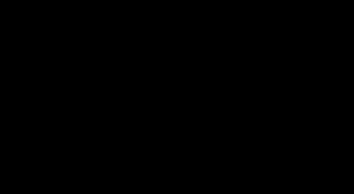
\includegraphics[width=0.7\linewidth]{optocoupler_clearance.pdf}
          \caption{K pojmu external creepage a clearance}
          \label{es:fig_optocoupler_clearance}
        \end{figure}

%} % tikzset
%---------------------------------------------------------------------------------------------------
%=============== Seznam literatury ===============================================================
\printbibliography[title={Seznam literatury}, heading=bibliography]
}  % DEBUG was off
%--------------------------------------------------------------------------------------------------
%                            /$$      /$$  /$$$$$$   /$$$$$$          /$$   /$$                                   | $$$    /$$$ /$$__  $$ /$$__  $$
%                           | $$$    /$$$ /$$__  $$ /$$__  $$        | $$$ | $$                                   | $$$$  /$$$$| $$  \ $$| $$  \__/
%                           | $$$$  /$$$$| $$  \ $$| $$  \__/        | $$$$| $$                                   | $$ $$/$$ $$| $$$$$$$$| $$ /$$$$
%                           | $$ $$/$$ $$| $$$$$$$$| $$ /$$$$ /$$$$$$| $$ $$ $$                                   /$$      /$$  /$$$$$$   /$$$$$$ 
%                           | $$  $$$| $$| $$__  $$| $$|_  $$|______/| $$  $$$$                                   | $$  $$$| $$| $$__  $$| $$|_  $$
%                           | $$\  $ | $$| $$  | $$| $$  \ $$        | $$\  $$$                                   | $$\  $ | $$| $$  | $$| $$  \ $$
%                           | $$ \/  | $$| $$  | $$|  $$$$$$/        | $$ \  $$                                   | $$ \/  | $$| $$  | $$|  $$$$$$/
%                           |__/     |__/|__/  |__/ \______/         |__/  \__/                                   |__/     |__/|__/  |__/ \______/                    
%--------------------------------------------------------------------------------------------------
\ifthenelse{ \equal{\DebugMode}{true} }{% Debug mode ON
  % !TeX spellcheck = cs_CZ
%file:spojity_model_elmag_p.tex
%{\tikzset{external/prefix={tikz/TEO/}}
% \tikzset{external/figure name/.add={ch01_}{}}
%==============================Kapitola: Spojité matematické modely jednotlivých polí ==============
\chapter{Spojité matematické modely polí}
\minitoc
  \section{Elektromagnetické pole}       
    \subsection{Veličiny elektromagnetického pole a jejich jednotky}
      \fbox{Elektrický náboj} je \emph{skalární veličinou}. Jednotkou je \emph{coulomb [C]}. Má
         kvantový charakter (tj. je roven celistvému násobku elementárního náboje $e =
         1,602\cdot10^{-19}C$), avšak v technických aplikacích k tomu nepřihlížíme. Náboj $Q$
         může být rozložen:
         \begin{itemize}\addtolength{\itemsep}{-0.5\baselineskip}
            \item \emph{prostorově} v objemu $V$ s objemovou hustotou
               \begin{equation}\label{TEMP:eq_q_varrho}
                  \varrho = \frac{dQ}{dV} \qquad [C\cdot m^{-3}]
               \end{equation}               
            \item \emph{plošně} na ploše $S$, s plošnou hustotou
               \begin{equation}\label{TEMP:eq_q_sigma}
                  \sigma = \frac{dQ}{dS} \qquad [C\cdot m^{-2}]
               \end{equation}                 
            \item \emph{lineárně} na křivce $l$, s lineární hustotou
               \begin{equation}\label{TEMP:eq_q_tau}
                  \tau = \frac{dQ}{dl} \qquad [C\cdot m^{-1}]
               \end{equation}                 
         \end{itemize}
         Rozlišujeme:
           \begin{itemize}\addtolength{\itemsep}{-0.5\baselineskip}
             \item \textbf{volné náboje}: mohou se přemisťovat v makroskopických
             vzdálenostech,
             \item \textbf{vázané náboje}: mohou se přemisťovat jen v
             mikroskopických vzdálenostech.
           \end{itemize}
         Volnými náboji jsou volné elektrony v kovech nebo ionty v elektrolytech (jsou odpoutány od
         atomů, resp. molekul a volně se mezi nimi pohybují); vázané náboje vznikají polarizací
         dielektrika.
         
      \vspace{1em}
      \fbox{Elektrický proud}\label{TEMP:kap_el_proud_velicina} je znám z každodenního života,
        přesto je velmi důležité umět tento pojem vnímat jak pro označení „jevu“ (kap.
        \ref{TEMP:kap_elproud_jev}), tak jako fyzikální veličinu, která tento jev kvantitativně
        popisuje (kap. \ref{TEMP:kap_el_proud_velicina} ). Elektrický proud je \emph{skalární
        fyzikální veličina} tzn. $I$ resp. $i$, jejíž jednotkou je základní jednotka soustavy SI:
        \emph{ampér} – [A]. V této soustavě jednotek je ampér definován na základě silových
        účinků mezi dvěma vodiči, kterými prochází elektrický proud. Tato síla je magnetického
        původu, avšak magnetické pole vzniká jako důsledek pohybu elektrického náboje.Je tvořen
        uspořádaným pohybem elektrických nábojů.
        
        Připojíme-li vodič ke zdroji elektrického napětí, elektrické pole uvnitř působí elektrickou
        silou na vodivostní elektrony, vyvolává jejich pohyb a tím vytváří elektrický proud, který
        je po krátké době \emph{stacionární} (ustálený, nezávislý na čase). Jestliže vodičem projde
        náboj $\Delta Q$ resp. $dQ$ za časový interval $\Delta t$ resp. $dt$, lze definovat
        \emph{průměrný} resp. \emph{okamžitý} proud ve vodiči:
        \begin{itemize}\addtolength{\itemsep}{-0.5\baselineskip}
          \item \textbf{průměrný} elektrický proud: $$I_{AV} = \frac{\Delta Q}{\Delta t}
                \qquad[A],$$
          \item \textbf{okamžitý} elektrický proud (který je limitním případem proudu průměrného,
                studujeme-li množství náboje, které projde průřezem vodiče za infinitezimální
                (nekonečně krátký) časový interval): $$i = \lim_{\Delta t \rightarrow 0}\frac{\Delta
                Q}{\Delta t} = \frac{dQ}{dt} \qquad[A].$$ V ustáleném stavu protéká všemi průřezy
                vodiče stejně velký proud,
          \item speciálně pohybuje-li se náboj vodičem rovnoměrně, nazýváme proud
                \textbf{stejno\-směr\-ným}, $I(t) = \text{konst}$, a platí $$ I_{DC} =
                \frac{Q}{t}\qquad[A] $$
        \end{itemize}        

        Elektrický proud jako \emph{jev} charakterizuje jednu z forem fyzikálního pohybu, kterou je
        \textbf{uspořádaný pohyb elektricky nabitých částic} v látce. Přestože jakýkoliv elektrický
        proud je vždy tvořen pohybujícími se náboji, nemusí všechny pohybující se náboje vytvářet
        elektrický proud. Ve vodiči dochází ke vzniku trvalého elektrického proudu za těchto
        podmínek:
          \begin{itemize}\addtolength{\itemsep}{-0.5\baselineskip}
            \item vodič se musí nacházet v trvalém elektrickém poli, což je realizováno pomocí tzv.
                  \emph{zdroje} (generátoru) elektrického napětí,
            \item ve vodiči musí být přítomny volné nosiče elektrického náboje.
          \end{itemize}
        
        Podle charakteru vnějšího elektrického pole lze rozlišit tři základní druhy proudů:
          \begin{labeling}{stejnosměrný}\addtolength{\itemsep}{-0.5\baselineskip}
            \item[\textbf{stejnosměrný}] proud vzniká tehdy, jestliže má intenzita elektrického pole
                   konstantní orientaci,
            \item[\textbf{střídavý}] proud ve vodiči vytváří vnější elektrické pole, jehož intenzita
                  periodicky mění svou orientaci na opačnou,
            \item[\textbf{stacionární}] stejnosměrný proud vzniká ve vodiči, je-li intenzita
                  elektrického pole konstantní co do velikosti, směru i orientace.
          \end{labeling}  

       Nabité částice představující volný náboj ve vodičích jsou v neustálém chaotickém tepelném
       pohybu (viz molekulová fyzika a termodynamika). Jedná se o \emph{mikroskopický pohyb}, který
       nemá za následek makroskopicky pozorovatelné přemístění náboje. Pokud ve vodiči vytvoříme
       elektrické pole, tepelný pohyb nabitých částic neustane, ale k náhodné složce rychlosti
       přibude ještě složka rychlosti ve směru vloženého pole.
       
       Při studiu elektrického proudu v kovových vodičích se zabýváme ustálenými proudy
       vodivostních elektronů, které v kovu vytváří tzv. \emph{elektronový plyn}. Tyto vodivostní
       elektrony jsou téměř volné a pohybují se v poli kladných iontů uspořádaných v krystalové
       mřížce.
        
       Experimentálně lze elektromagnetické pole prokázat silovým působením na elektricky nabité
       částice. Celkovou sílu $\vec{F}$ lze rozložit na elektrickou sílu $\vec{F}_e$, nezávislou na
       tom, zda je nabitá částice v klidu nebo v pohybu vůči vztažné soustavě a na magnetickou sílu
       $\vec{F}_m$, působící jen na pohybující se částice. Elektromagnetické pole má tedy dvě
       složky: \textbf{elektrické pole}, působící na náboj silou $\vec{F}_e$ a \textbf{magnetické
       pole}, působící na pohybující se náboj silou $\vec{F}_m$  \cite[s.~13]{Mayer2001}.
      
      \vspace{1em}
      \fbox{Intenzita elektrického pole $\vec{E}$} je vektorovou veličinou charakterizující
        \emph{elektrické pole}.
        Je definována jako 
        \emph{síla působící na nepohybující se jednotkový bodový náboj}:
        \begin{equation}\label{TEMP:eq_E}
          \vec{E} = \frac{\vec{F}_e}{Q} \qquad\left[\frac{V}{m}\right]  
        \end{equation}        
        kde $\vec{F}_e$ je elektrická síla působící na náboj $Q$.
      
      \vspace{1em}
      \fbox{Magnetická indukce $\vec{B}$} je vektorovou veličinou charakterizující \emph{magnetické
        pole}. Je definovována vztahem
        \begin{equation}\label{TEMP:eq_B}
          \vec{F}_m = Q(\vec{v}\times\vec{B}) \qquad[T]  
        \end{equation}        
        kde $\vec{F}_m$ je magnetická síla působící na náboj $Q$ pohybující se rychlostí $\vec{v}$.
        Jednotkou je \emph{tesla} $[T]$.
    
        Síla, jež působí elektromagnetické pole na pohybující se náboj se nazývá \textbf{Lorentzova
        síla}
        \begin{equation}\label{TEMP:eq_Lorentz}
          \vec{F} = \vec{F}_e + \vec{F}_m =Q(\vec{E} + \vec{v}\times\vec{B}) \qquad[N]  
        \end{equation}        

    \subsection{Maxwellovy rovnice}
      Makroskopická teorie elektromagnetického pole v klasickém pojetí vychází ze základních zákonů
      vyjádřených \emph{Maxwellovými rovnicemi (MR)}. Lze je zapsat buď v \textbf{integrálním},
      nebo \textbf{diferenciálním tvaru}. V integrálním tvaru popisují elektromagnetické pole v
      jisté prostorové oblasti $\Omega$, kdežto v diferenciálním tvaru ve vnitřním bodě této
      oblasti. Soustavu vlastních MR představují první čtyři páry rovnic; často se k nim připojuje
      jako další základní rovnice elektromagnetického pole rovnice kontinuity pro vodivý proud.
      Její integrální a diferenciální tvar reprezentují poslední dvě rovnice.
exa
      \begin{align}
        \oint_\mathcal{C}\vr{H} d\vr{l} &= I+\der{\Psi}{t}
                                           \quad \rot{H}=\vr{J}+\pder{\vr{D}}{t}             \\
        \oint_\mathcal{C}\vr{E} d\vr{l} &= -\der{\Phi}{t}
                               \qquad \rot{E}=-\pder{\vr{B}}{t}\\
         \int_\mathcal{S}\vr{D} d\vr{S} &= Q \qquad\quad\;   \diver{D}=\rho_V                \\
         \int_\mathcal{S}\vr{B} d\vr{S} &= 0 \qquad\quad\;\; \diver{B}=0                     \\
         \int_\mathcal{S}\vr{J} d\vr{S} &= -\der{Q}{t} \quad\;\;\;\diver{J}=-\der{\rho_V}{t}
      \end{align}

      Předpokládá se, že \emph{všechny křivky a plochy v integrálním tvaru MR jsou po částech
      hladké a všechny integrované veličiny jsou po částech spojité funkce}. Pak je zaručena
      existence integrálů v těchto rovnicích. V diferenciálním tvaru MR se předpokládají pouze
      \textbf{regulární body} oblastí, což jsou body, v nichž jsou veličiny $\vr{E}$, $\vr{D}$,
      $\vr{B}$ a $\vr{H}$ \emph{spojité a spojitě diferencovatelné funkce}; nejsou jimi tedy např.
      body rozhraní dvou různých prostředí, v elektrickém poli body v nichž jsou umístěny diskrétní
      náboje, v magnetickém poli body proudových vláken atd.

      % --------example: Energie v Kondenzátoru ------------------------
      % \label{TEO:exam019}
      % !TeX spellcheck = cs_CZ
\begin{example}\label{teo:exam019}
  Mějme nabitý deskový kondenzátor \(C\), zobrazený na obr. \ref{teo:fig019a}. Zvětšme jeho
  kapacitu, například tím, že zvětšíme plochu jeho elektrod, nebo připojíme paralelně druhý stejné 
  velikosti, viz obr. \ref{teo:fig019b}. Otázka zní, jak velká enerige bude uložena v 
  elektrostatickém poli obou kondeznátorů? Bude energie po rozdělení náboje mezi oba 
  kondenzátory rovna původní energií nabitého kondenzátoru? Pokud ne, vysvětlete kam se část 
  energie transformovala. 
  
   {\centering
    \captionsetup{type=figure}
    \begin{tabular}{cc}
     \subfloat[ ]{\label{teo:fig019a}
       \includegraphics[width=0.15\linewidth]{teo_fig019a.png}}              &
     \hspace{3em}
     \subfloat[ ]{\label{teo:fig019b}
       \includegraphics[width=0.5\linewidth]{teo_fig019b.png}}
    \end{tabular}
    \captionof{figure}{K příkladu \ref{teo:exam019}: a) Nabitý kondenzátor s rovnoběžnými rovinnými 
    elektrodami; b) Rozložení náboje na obou kondenzátorech velikosti}
    \label{teo:fig019}
  \par}
  
  Je-li dielektrikum kondenzátoru lineární, pak pro energii elektrického pole akumulovanou v 
  nabitém kondenzátoru platí. Podrobněji například v kapitole \ref{fyz:IIchapVsecXIX}.
  \begin{equation}
    W = \frac{1}{2}CU^2 \quad\text{nebo}\quad W = \frac{1}{2}\frac{Q^2}{C} 
    \quad\text{kde}\quad C = \frac{Q}{U}
  \end{equation}
  Předpokládejme ustálený stav po připojení druhého kondenzátoru, jak je znázorněno na obr. 
  \ref{teo:fig019b}. V obvodu nepředpokládáme přítomnost odporu, který by způsobil ztrátu energie, 
  vyzářené v podobě tepla. Kapacita je dvojnásobná a náboj zůstal stejný. Na každém kondenzátoru 
  tedy očekáváme polovinu původního náboje. Sečteme-li energii uloženou v elektrických polích obou 
  kondenzátorů dostaneme
  \begin{align*}
    W^* &= \frac{1}{2}\frac{(\frac{1}{2}Q)^2}{C} + \frac{1}{2}\frac{(\frac{1}{2}Q)^2}{C} 
         = \frac{(\frac{1}{2}Q)^2}{C} =\frac{1}{4}\frac{Q^2}{C}                               \\
        &  \xrightarrow[\scriptscriptstyle{C\rightarrow2C}]{}
           \frac{1}{2}\frac{Q^2}{(2C)} = \frac{1}{2}W 
  \end{align*}
  Kupodivu, polovina energie prostě chybí a jelikož platí zákon zachování energie\footnote{viz 
  partie Fyzika \ref{part:FYZI}, kapitola \ref{fyz:IchapII})}, nezbývá nic jiného než uznat, že 
  elektrický obvod dle \ref{teo:fig019b}, nemodeluje fyzikální problém dost věrně. Tím jsme dospěli 
  k závěru, že je nutné do obvodu dodat rezistor, tak jak je znázorněno na obrázku   
  \ref{teo:fig020}.
  
   {\centering
    \captionsetup{type=figure}
    \includegraphics[width=0.4\linewidth]{teo_fig020.png}
    \captionof{figure}{Rezistor \(R\) představuje ztráty, které nebyly v obvodu na obrázku 
               \ref{teo:fig019b} předpokládány}
    \label{teo:fig020}
  \par}
  
  Abychom mohli určit teplné ztráty na rezistoru dané integrálem \(\int_{0}^{\infty} 
  Ri^2(t)\dd{t}\), nedříve sestavíme jednoduchou diferenciální rovnici prvního řádu aplikací II. 
  Kirchhoffova zákona, ze které odvodíme vzorec pro časovou závislost proudu \(i(t)\). 
  \begin{align*}
    \frac{Q_0 - Q}{C} - Ri(t) - \frac{Q_0}{C}         &= 0 \quad/\der{ }{t}             \\
    \frac{-i(t)}{C} - R\der{i(t)}{t} - \frac{i(t)}{C} &= 0                              \\
                                        \der{i(t)}{t} &= - \frac{2}{RC}i(t) \quad/\int  \\
                                                 i(t) &= I_0e^{-\frac{2}{RC}t}
  \end{align*}
  Nyní můžeme stanovit energii disipované na rezitoru \(R\)
  \begin{align*}
    W   &= \int_{0}^{\infty}Ri^2(t)\dd{t} = RI_0^2\int_{0}^{\infty}e^{-\frac{4}{RC}t}\dd{t}   \\
    \shortintertext{Do integrované funkce dosadíme novou proměnnou \(u = \frac{4}{RC}t\), \(\dd{u} 
                    = \frac{4}{RC}\dd{t}\), \(\dd{t} = \frac{RC}{4}\dd{u}\)}
        &= RI_0^2\int_{0}^{\infty}e^{-u}\frac{RC}{4}\dd{u} 
         = R^2I_0^2\frac{C}{4}\underbrace{\int_{0}^{\infty}e^{-u}\dd{u}}_1  \\
    \shortintertext{Jelikož platí \(I_0 = \frac{U}{R}=\frac{Q}{CR}\) dostaneme po dosazení}
        &= \cancel{R^2}\frac{Q^2}{C^2\cancel{R^2}}\frac{C}{4} = \frac{Q^2}{4C}
         = \frac{1}{2}W
  \end{align*}
  Nyní je vše v pořádku. Druhá polovina energie je disipována na rezistoru a navíc z výsledku 
  vyplývá, že vubec nezávisí na \(R\)!
\end{example}


  
      %-----------------------------------------------------------------
      
  % --------------- Stacionární magnetické pole-----------------------------------------------------
  \section{Stacionární proudové pole}
    V elektrostatice (tj. elektrickém poli nepohybujících se nábojů) neexistuje trvalý elektrický
    proud. Zdroje napětí (galvanické články, termočlánky, dynama aj.) mají tu vlastnost, že na
    jejich záporné svorce je trvale nadbytek elektronů, a na jejich kladné svorce jejich
    nedostatek. Těmito zdroji můžeme ve vodiči trvale udržovat elektrické pole a tedy i tok nosičů
    elektřiny. Jestliže se \emph{náboje pohybují konstantní rychlostí, hovoříme o stacionárním
    elektrickém proudu}. Základní rovnice elektrostatické pole jsou:

    \begin{table}[ht!]
      \setlength\extrarowheight{5pt}
      \centering
      \begin{tabular}{lc|c|}
        \cline{2-3}
        \multicolumn{1}{l|}{} 
          & \textbf{integrální tvar} & \textbf{diferenciální tvar}                    \\[8pt]
        \hline
        \multicolumn{1}{|l|}{2. MR} 
          & \(\bigointsss\vr{E}\cdot d\vr{l} = 0\) & \(\rot{E} = 0\)                  \\[8pt] 
        \cline{1-3}
        \hline
        \multicolumn{1}{|l|}{Zákon kontinuity} 
          & \(\bigointsss\vr{J}\cdot d\vr{S}=0\) & \(\diver{J}=0\)                    \\[8pt]
        \cline{1-3}
        \multicolumn{1}{|l|}{Ohmův zákon}
          & \(I=GU=\dfrac{U}{R}\) & \(\vr{J} = \gamma\vr{E} = \dfrac{1}{\rho}\vr{E}\) \\[8pt]
        \cline{1-3}
      \end{tabular}
      \caption{Základní rovnice stacionárního proudového pole}
    \end{table}
    
    \subsection{Elektrický proud v kovových vodičích}\label{TEMP:kap_elproud_jev}
      V předchozí kapitole \ref{TEMP:kap_el_proud_velicina} bylo o elektrickém proudu pojednáváno
      jako o skalární fyzikální veličině. V této kapitole nás bude zajímat makroskopický pohled na
      „jev“ známý jako \emph{elektrický proud}.
      
      Zopakujme, že elektrickým proudem je míněn uspořádaný pohyb elektrických ná\-bo\-jů, a aby se
      tyto náboje mohly pohybovat, musí být volné - jsou přítomny v látkách, které nazýváme
      \textbf{vodiče}. Vodiče mohou mít nositele náboje jednoho znaménka (elektrony v kovech,
      uhlíku a v polovodičových) anebo obojích znamének (kladné a záporné ionty v elektrolytech,
      ionty a elektrony v ionizovaných plynech). Volné nositele náboje (elektrony, ionty) lze
      rovněž oddělit od těchto látek (vodičů) a vytvořit elektrický proud ve vakuu nebo ve
      zředěných plynech.
      
      Z vodičů mají největší význam \textbf{kovy}, které jsou polykrystalickými látkami s kovovou
      vazbou. Každý mikroskopický monokrystal kovu má pevnou krystalovou mříž sestavenou z kladných
      iontů, mezi nimiž se přetržitě pohybují \emph{volné elektrony} rychlost\-mi, jejichž velikost
      je statisticky proměnná (co do velikosti i směru). Střední hodnota rychlosti (jako vektoru)
      všech elektronů je nulová. Střední hodnota rychlosti určitého elektronu je závislá na teplotě
      vodiče. Elektrony konají tzv. \emph{termický pohyb}. Rychlosti neuspořádaných termických
      pohybů dosahují jen o několik řádů větších hodnot, než kmity iontů v krystalech mřížky.

      \begin{figure}
        \centering
        \includegraphics[width=0.5\linewidth]{vd_e_drift.pdf}
        \caption[Pohyb elektronu ve vodiči.]{Pohyb elektronu ve vodiči. Fyzikálně je $v_d$ 
                 průměrná rychlost nosičů náboje uvnitř vodiče, který je vložen do vnějšího
                 elektrického pole. Ve skutečnosti se ale elektron ve vodiči nepohybuje po přímce,
                 jeho pohyb je chaotický.}
        \label{TEMP:fig_vd_e_drift}
      \end{figure}
      
      Připojíme-li vodič k vnějšímu zdroji elektrického pole (např. ke galvanickému článku), začne
      statisticky převládat uspořádaný pohyb nosičů kladného (záporného) náboje ve směru (proti
      směru) vnějšího pole nad termickým pohybem, což v makroskopickém měřít\-ku pozorujeme jako
      \textbf{makroskopický elektrický proud}. Jsou-li ve vodiči přítomny nosiče náboje obou
      polarit, dojde k pohybu ve vzájemně opačných směrech, přičemž směr toku nosičů kladného
      náboje se historicky ztotožňuje se směrem toku elektrického proudu. U kovových vodičů je tedy
      směr proudu právě opačný, než směr toku elektronů, jenž tento elektrický proud tvoří.
      
      Velikost (intenzitu) proudu posuzujeme podle velikosti náboje obojí polarity, který projde
      určitým průřezem vodiče ve vzájemně opačných směrech za jednotku času. Projde-li průřezem
      vodiče celkově náboj $dQ$ za čas $dt$, bude tok náboje vodičem charakterizovat skalární
      veličina
        \begin{equation}\label{TEMP:eq_I_01}
          I = \frac{dQ}{dt} \qquad[A],  
        \end{equation}        
      která se nazývá \emph{elektrický proud}($1C\cdot s^{-1} = 1A $ čteno \emph{ampér}). Tato
      jednotka patří mezi základní jednotky \texttt{SI} soustavy.
      
      Pro \emph{stacionární} (tj. časově neproměnný - ustálený) proud můžeme obecný výraz
      \ref{TEMP:eq_I_01} nahradit rovnicí
        \begin{equation}\label{TEMP:eq_I_02}
          I = \frac{Q}{t}.  
        \end{equation}       
      Jedná-li se o rovnoměrný pohyb bodového náboje $Q$ po kružnici s periodou $T$, resp. s
      úhlovou rychlostí $\omega$, můžeme vzniklý ustálený proud vyjádřit rovnicí 
        \begin{equation}\label{TEMP:eq_I_03}
          I = \frac{Q}{T} = \frac{\omega Q}{2\pi}.  
        \end{equation}
      
      Bude-li se element náboje $dQ$ pohybovat v lineárním útvaru rychlostí $v = \frac{dQ}{dl}$,
      bude po dosazení do rov.\ref{TEMP:eq_I_01} reprezentovat elektrický proud 
        \begin{equation}\label{TEMP:eq_I_04}
          I = \frac{dQ}{dt} = \frac{dQ}{dl}v = \tau v, 
        \end{equation}      
      kde $\tau$ je \emph{délková hustota} náboje a $v$ je velikost \emph{okamžité rychlosti}
      náboje v uvažovaném místě lineárního útvaru. 

      \begin{figure}[ht!]
         \centering
         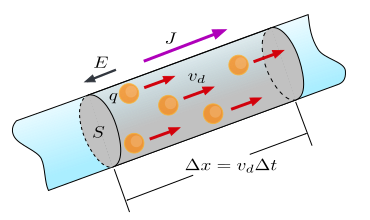
\includegraphics[width=0.5\linewidth]{el_proud_ve_vodici.pdf}
         \caption[Náboje, pohybující se vodičem]{Směr elektrického proudu byl implicitně stanoven
                  jako směr pohybu kladných nábojů. Nositeli elektrického náboje uvnitř vodičů jsou
                  ovšem záporně nabité volné elektrony, které se tedy dle  konvence pohybují proti
                  směru elektrického proudu. Elektrický proud může protékat pevnými látkami (kovy,
                  polovodiči), kapalinami (elektrolyty) a ionizovanými plyny. Látky, které nevedou
                  elektrický proud, nazýváme nevodiči, izolanty}
         \label{TEMP:fig_el_proud_ve_vodici}
      \end{figure}
      
      Elektrický proud je veličina, která obecně popisuje prostorový jev. Omezíme se nyní na běžný
      případ vodiče, jako je na obr. \ref{TEMP:fig_el_proud_ve_vodici}, který má volné náboje jen
      jedné polarity (u kovových vodičů jde o elektrony) a označme $\rho_0$ prostorovou hustotu
      volného náboje a $v_d$ velikost usměrněné rychlosti jejich nositelů (elektronů). Pak za čas
      $dt$ projde průřezem o obsahu $S_0$ ($S_0\bot v_d$) náboj $dQ = \rho_0 S_0 v_d dt$.
      Elektrický proud vyjádřený rov.
      \ref{TEMP:eq_I_01} můžeme přepsat do tvaru
        \begin{equation}\label{TEMP:eq_I_05}
          I = \rho_0 S_0 v_d = - e n_0 S_0 v_d, 
        \end{equation}         
      kde $\displaystyle{n_0 = \frac{\rho_0}{-e}}$ je počet nositelů volného náboje (tj. v našem
      případě elektronů, z nichž každý nese náboj $-e$ v jednotkovém objemu vodiče, přičemž pro
      elektrony zřejmě je $\rho_0<0$.

      \begin{wrapfigure}[14]{r}{5cm}
        \centering
        \includegraphics[width=0.9\linewidth]{plocha_S.pdf}
        \caption[Rovinná plocha $S$.]{Rovinná plocha $S = S_0\cos\alpha$}
        \label{TEMP:fig_plocha_S}
      \end{wrapfigure}
      Rovinnou plochou $S$ průřezu můžeme zavést jako vektor $vr{S}$, který má směr daný normálou k
      ploše a pravidlem pravé ruky (ukazují-li prsty pravé ruky směr oběhu po hraniční křivce
      plochy, ukáže palec směr plochy jako vektoru $\vr{S}$). Protože driftová rychlost $v_d$ je
      také vektor, nebudeme obecně uvažovat vektory $\vr{S}, \vr{v_d}$ o stejném směru a rovnici
      \ref{TEMP:eq_I_05} přepíšeme do obecnějšího tvaru      
      
      \begin{equation}\label{TEMP:eq_I_06}
        I = \rho_0 \vr{S_0}\cdot\vr{v}_d = jS\cos\alpha = jS_0, 
      \end{equation}      
      kde $S_0 = S$ pro $\alpha = 0$ (viz obr. \ref{TEMP:fig_plocha_S}) a   
      \begin{equation}\label{TEMP:eq_I_07}
        \vr{j} = \rho_0\vr{v_d}, 
      \end{equation}        
      je proudová hustota. Je to vektor o velikosti 
      \begin{equation}\label{TEMP:eq_I_08}
        j = \frac{I}{S\cos\alpha} = \frac{I}{S_0}  \qquad A\cdot m^{-2}, 
      \end{equation}   
      obecněji
      \begin{equation}\label{TEMP:eq_I_09}
        j = \frac{dI}{dS}, 
      \end{equation}

      a o směru vektoru driftové rychlosti nositelů kladného náboje. Pro případ nositelů volného
      náboje - elektronů má proudová hustota opačný směr než driftová rychlost $v_d$ (obr.
      \ref{TEMP:fig_plocha_S}).
      
      Velikost vektoru $\vr{j}$ má význam plošné hustoty elektrického proudu v uvažovaném místě
      průřezu. Jednotkou je $A\cdot m^{-2}$.
      
      Nebude-li proudová hustota na uvažovaném průřezu konstantní, bude celkový elektrický proud
      procházející průřezem o obsahu $S$ dán integrálem 
        \begin{equation}\label{TEMP:eq_I_10}
          I = \int_S \vr{j}d\vr{S}. 
        \end{equation} 

      % --------example: Driftová rychlost elektroknů ve vodiči --------
      % \label{TEO:exam008}
      % !TeX spellcheck = cs_CZ
%---------- Driftová rychlost elektroknů ve vodiči: 
\begin{mdframed}[style=mdexam]
\begin{example}\label{TEO:exam008} \emph{Driftová rychlost elektronů ve vodiči:} Vodičem z 
jednomocné mědi o
  průřezu $S_0 = \SI{1}{\mm^2}$ prochází elektrický proud $I = \SI{5}{\A}$. Vypočtěte:
  \begin{itemize}[noitemsep, leftmargin=2em]
    \item počet volných elektronů v jednotkovém objemu \ce{Cu},
    \item úhrnný náboj volných elektronů v jednotkovém objemu,
    \item driftovou rychlost volných elektronů při proudu \(I\).
  \end{itemize}
  Měď má poměrnou atomovou hmotnost $A_r = 63,54$ a hustotu\footnote{Pro hustotu budeme používat 
  alternativní značku $s$, s ohledem na kolizi značky $\rho$, jež označuje hustotu náboje.} $s = 
  \SI{8.93e3}{\kg.\m^{-3}}$.\newline  
  \textbf{Řešení:}
  \begin{itemize}[leftmargin=2em]
    \item Jeden mol mědi o molové hmotnosti $M = \SI{0.06354}{\kg\per\mol}$ a o molovém
          objemu 
          \begin{align*}
            V_m &= \frac{M}{s} 
                 = \frac{\SI{63.54e-3}{\kg.\mol^{-1}}}{\SI{8.93e3}{\kg.\m^{-3}}}      \\
                &= \SI{7.12e-6}{\m^3.\mol^{-1}}
          \end{align*}
          obsahuje $N_A = 6,0221\cdot10^{23}$ jednoatomových molekul \emph{Cu} na jeden mol,
          z nichž každý má volný jeden (valenční) elektron. Tedy počet volných elektronů v
          jednotkovém objemu je 
          \begin{align*}
            n_0 &= \frac{N_A}{V_m} = \frac{sN_A}{M}                                           
                 = \frac{\SI{6.0221e23}{\mol^{-1}}}{\SI{7.12e-6}{\m^{3}.\mol^{-1}}}    \\
                &= \SI{8.46e28}{\per\cubic\m}.
          \end{align*}  
    \item Úhrnný náboj volných elektronů v jednotkovém objemu mědi je 
          \begin{equation}
            Q_v = -e\cdot n_0 = \SI{-1.36e10}{\coulomb.m^{-3}}.
          \end{equation}
    \item Velikost driftové rychlosti určíme ze vztahu $I = -en_0v_dS_0 = - Q_v v_d S_0$ tj.
    \begin{align*}
      v_d &= \left\lvert\frac{I}{Q_v\cdot S_0}\right\rvert                       
           = \frac{\SI{5}{\coulomb\per\s}}{\SI{1.36e10}{\coulomb.m^{-3}}\cdot\SI{1e-6}{\m^2}}   \\
          &= \SI{3676e-4}{\m\per\s} = \SI{0.3676}{\mm\per\s}.  
    \end{align*}
  \end{itemize}
  Z provedených výpočtů si můžeme udělat názor o mikroskopických poměrech v kovových vodičích: počet
  volných nositelů náboje - elektronů a jejich úhrný náboj v jednotkovém objemu je značný a proto
  driftová rychlost elektronů potřebná k vyvolání proudu běžné velikosti v drátových vodičích je
  nesmírně malá (doslova hlemýždí).
\end{example}  
\end{mdframed}
  
      %-----------------------------------------------------------------

      % --------example: Velikost náboje v minci -----------------------
      % \label{TEO:exam009}
      % !TeX spellcheck = cs_CZ
%---------- Velikost náboje v minvi:
\begin{example}
  Elektricky neutrální měděná mince o hmotnosti \(m = \SI{3.11}{\g}\) obsahuje stejné množství 
  kladného a záporného náboje. Jaké je velikost kladného (nebo záporného) náboje obsaženého v 
  minci?\newline  
  \textbf{Řešení:}\newline
  Neutrální atom má záporný náboj \(Z\cdot e\), představovaný jeho elektrony a kladný náboj o 
  stejné velikosti představovaný protony v jádře. Pro měď je atomové číslo \(Z\) rovno \num{29}, 
  tj. atom mědi má \num{29} protonů, a je-li elektricky neutrální, také \num{29} elektronů.
  
  Náboj o velikosti \(Q_v\), který hledáme je roven \(N\cdot Z\cdot e\), kde \(N\) je počet atomů 
  obsažených v  jednom molu (Avogadrova konstanta: \(N_A = \SI{6.0221e23}{\per\mole}\)). Počet 
  molů mědi v minci \(\frac{m}{M}\), kde \(M = \SI{63.5}{\g\per\mole}\) je molární hmotnosti mědi: 
  \begin{equation*}
    N = N_A\cdot\frac{m}{M} = \SI{6.0221e23}{\per\mole}
           \frac{\SI{3.11}{\g}}{\SI{63.5}{\g\per\mole}} 
      = \num{2.95e22}.
  \end{equation*}
 Velikost celkového kladného (záporného) náboje v minci je pak 
  \begin{equation*}
    Q_v = N\cdot Z\cdot e = \num{2.95e22}\cdot\num{29}\cdot\SI{1.602e-19}{\coulomb} 
        = \SI{137039}{\coulomb}
  \end{equation*}
  To je obrovský náboj. Pro srovnání: třeme-li ebonitovou tyč vlněnou látkou, můžeme na tyč 
  přemístit stěží náboj o velikosti \SI{1e-9}{\coulomb}.
\end{example} 
  
      %-----------------------------------------------------------------

    % ----------------Práce a výkon elektrického proudu-----------------
    \subsection{Práce a výkon elektrického proudu}
      % --------example: Ponorný vařič ---------------------------------
      % \label{TEO:exam010}
      % !TeX spellcheck = cs_CZ
%---------- Ponorný vařič:
\begin{mdframed}[style=mdexam]
  \begin{example}\label{TEO:exam010}
    Za jakou dobu uvede norný vodič o příkonu \SI{600}{\W} do varu \SI{1}{\litre} vody o počáteční
    teplotě $\SI{20}{\degreeCelsius}$. Uvažujte měrnou tepelnou kapacitu vody $c =
    \SI{4200}{\joule\per\kg\per\K}$. Výměnu tepla s okolím neuvažujte.
    \newline 
    \textbf{Řešení:}\newline Pro var vody bude zapotřebí tepla dle rovnice $Q  = m\cdot c\cdot(T_2 -
    T_1)$. Potřebná elektrická práce je $Q_e = P\cdot t = U\cdot I\cdot t$ a tedy dobu ohřevu
    stanovíme z rovnice:
    
    {\centering
    \captionsetup{type=figure}
    \luafigure[0.3]{teo_fig033.png}
    \captionof{figure}{Ilustrace k příkladu \ref{TEO:exam010}}
    \label{teo:fig033}
    \par}

    \begin{align*}
      P\cdot t &= m\cdot c\cdot(T_2 - T_1)                                               \\
             t &= \frac{m\cdot c}{P}\cdot(T_2 - T_1)                                     \\     
               &= \frac{\SI{1}{\kg}\cdot\SI{4200}{\joule\per\kg\per\K}}{\SI{600}{\W}}
                \cdot(\SI{100}{\degreeCelsius} - \SI{20}{\degreeCelsius})                \\ 
               &= \SI{560}{\s}.
    \end{align*}         
  \end{example}
\end{mdframed}  
      %-----------------------------------------------------------------
 
    % ----------------Ohmův zákon------------------------------------------------------------------
    \subsection{Ohmův zákon}
      Uvažujme vodič u něhož jsou volnými nositeli náboje \emph{elektrony}. Nyní v mezích klasické
      mechaniky kvantitativně popíšeme mechanismus vedení proudu, který povede k všeobecně známému
      \textbf{Ohmovu zákonu}
      
      Umístíme-li vodič do elektrického pole o intenzitě $\vec{E}$ (např. připojením ke
      galvanickému článku), působí na každý volný elektron síla $\vec{F} = -e\vec{E}$, která mu
      podle \emph{Newtonova zákona} udělí zrychlení $\vec{a} = \frac{\vec{F}}{m_e} = -
      \frac{e}{m_e}\vec{E}$ proti směru vnějšího pole. Tím získávají chaoticky se pohybující
      elektrony ještě složku rychlosti v protisměru vloženého elektrického pole $\vec{E}$ a  dojde
      tedy k usměrnění driftového pohybu volných elektronů a v souladu s kapitolou
      \ref{TEMP:kap_elproud_jev} pozorujeme, že ve vodiči vznikl makroskopický elektrický proud.
      
      Pohyb elektronu se ovšem neobejde bez srážek s ionty v krystalové mřížce. Dráhu, kterou se
      elektronu podaří urazit, nazýváme \emph{volnou dráhou} $d$. Průměrná doba mezi dvěma po sobě
      jdoucími srážkami nechť je $\tau$ za tuto dobu se bude elektron rovnoměrně urychlovat a těsně
      před následující srážkou jeho rychlost dosáhne maxima tj. $\vec{v}_{max} = \vec{a}\cdot\tau$.
      Nás ovšem zajímá průměrná rychlost (\emph{driftová rychlost})na volné dráze průměrné
      velikosti:
      \begin{equation}\label{TEMP:eq_vd_01}
        \vec{v}_d = \frac{\vec{v}_{max}}{2} = -\frac{e\tau}{2m_e}\vec{E}
      \end{equation}   
      Proudová hustota \ref{TEMP:eq_I_07} bude
      \begin{equation}\label{TEMP:eq_j_02}
        \vec{j} = \rho_0\vec{v}_d= -en_0\vec{v}_d = -\frac{e^2n_0\tau}{2m_e}\vec{E}
      \end{equation}       
      Koeficient úměrnosti 
      \begin{equation}\label{TEMP:eq_g_03}
        \gamma = \frac{e^2n_0\tau}{2m_e}
      \end{equation}     
      je závislý na počtů nositelů (elektronů) $n_0$ v jednotkovém objemu a na době $\tau$, neboli
      na délce volné dráhy. Veličina $\gamma$ se nazývá \emph{měrná elektrická vodivost} neboli
      \textbf{konduktivita} látky. Protože dobu $\tau$ nelze přímo měřit, určuje se $\gamma$
      experimentálně. Přitom se zjišťuje, že pro určitou teplotu zkoumané látky je $\gamma$
      konstantní.
      
      Po zavedení pojmu měrná elektrická vodivost látky \ref{TEMP:eq_g_03}, můžeme výraz
      \ref{TEMP:eq_j_02} přepsat do výsledného tvaru
      \begin{equation}\label{TEMP:eq_j_04}
        \vec{j} = \gamma\vec{E},
      \end{equation}              
      který se v literatuře označuje jako \emph{Ohmův zákon v diferenciálním tvaru} (i když se v
      pravém slova smyslu o diferenciální tvar nejedná). Výstižnější je označení \emph{lokální tvar
      Ohmova zákona}, protože výraz \ref{TEMP:eq_j_04} se vztahuje na určité místo, resp. bod,
      vodivého prostředí. Vztah říká, že proudová hustota v určitém bodě vodivého prostředí je
      přímo úměrná intenzitě vloženého elektrického pole v tomto bodě (platí pro určitou teplotu
      prostředí).
      
      Uvažujme nyní lineární homogenní vodič délky $l$ a příčného průřezu o obsahu $S_0$, připojený
      ke zdroji o napětí $U$. Pak intenzita pole uvnitř vodiče bude mít konstantní velikost
      $E=\frac{U}{l}$. Dosadíme-li za velikost proudové hustoty $j=\frac{I}{S_0}$ do
      \ref{TEMP:eq_j_04}, dostaneme vztah
      \begin{equation}\label{TEMP:eq_j_05}
        \frac{I}{S_0} = \gamma\frac{U}{l},
      \end{equation}        
      z něhož vyplývá známý vztah
      \begin{equation}\label{TEMP:eq_j_06}
        U = \frac{l}{\gamma S_0}I = RI,
      \end{equation}              
      kde
      \begin{equation}\label{TEMP:eq_j_07}
        R = \frac{l}{\gamma S_0} = \rho\frac{l}{S_0},
      \end{equation} 
      je \textbf{elektrický odpor} uvažovaného lineárního vodiče, přičemž $\rho = \frac{1}{\gamma}$
      je \emph{měrný elektrický odpor} (\textbf{rezistivita})\footnote{Zde je další kolize značky
      $\rho$. Nyní se tomuto problému vyhneme využíváním pouze konduktivity, jenž se častěji
      používá v teorii elektromagnetického pole.}. Výraz \ref{TEMP:eq_j_07} představuje klasický
      Ohmův zákon zákon experimentálně objevený r. 1826 \emph{G. S. Ohmem}. Jednotky:
      \begin{itemize}\addtolength{\itemsep}{-0.5\baselineskip}
        \item elektrický odpor: \si{V.A^{-1}},
        \item měrný elektrický odpor: \si{\ohm.m},
        \item měrná elektrická vodivost: \si{\ohm^{-1}.m^{-1}}.
      \end{itemize}

      % --------example: Ponorný vařič -----------------------
      % \label{TEO:exam011}
      % !TeX spellcheck = cs_CZ
\begin{example}
  \textbf{Zemnicí elektroda}: Uvažujte zemnicí elektrodu ve tvaru koule o poloměru  
  $a=\SI{200}{\mm}$, uloženou do zeminy v hloubce, která je značně větší než je poloměr $a$. Pro 
  jednoduchost řešení dále předpokládejte, že přívodní drát je od zeminy izolován (obr.
  \ref{TEMP:fig_zem_elektroda}). Zemina má měrnou vodivost $\gamma=\num[exponent-product =
  \cdot]{1,8e-2}\si{\per\ohm\per\m}$. Při zkratu teče přívodním drátem proud $I=\SI{50}{\A}$.
  Vypočítejte:
  
  %----------------------------------
  % image: TEMP_zem_elektroda.tex label: \label{TEMP:fig_zem_elektroda}
  \input{../src/TEO/img/TEMP_zem_elektroda.tex}  
  %----------------------------------         
  \begin{enumerate}[label=\emph{\alph*})]
    \item Závislost potenciálu $\varphi=\varphi(r)$ elektrického pole, které se vytvoří v
          zemině při zkratu, kde $r$ je vzdálenost od středu elektrody. Potenciál normujte
          volbou $\varphi(\infty)=0$.
    \item Zemnicí odpor elektrody, který je definován vztahem $$R_z=\frac{U_z}{I_z},$$ kde
          $U_z = \varphi(a)-\varphi(b)$ je zemnicí napětí 
    \item Ztrátový výkon při zkratu.            
  \end{enumerate}
  Řešení:    
  Ekvipotenciální a proudové plochy mají zřejmě kulový tvar se středem totožným s geometrickým 
  středem elektrody. Proudová hustota na kulové ploše obecného poloměru $r$ (viz. obr. 
  \ref{TEMP:fig_zem_elektroda}) je $$\vec{j}=\frac{I}{4\pi r^2}\vec{n},$$ kde $\vec{n}$ je 
  jednotkový vektor ve směru normály. Pak v bodech na této ploše musí být elektrické pole o 
  intenzitě $\vec{E}$, kterou určíme ze vztahu
  \begin{equation*}
    \vec{j}= \gamma\vec{E}\rightarrow\vec{E}=
    \frac{\vec{j}}{\gamma}=\frac{I}{4\pi\gamma r^2}\vec{n}.
  \end{equation*}
  Závislost potenciálu $\varphi=\varphi(r)$ tohoto elektrického pole stanovíme pomocí následujícího 
  integrálu
  \begin{equation}
    \varphi = - \int\vec{E}d\vec{r}+C = -\frac{I}{4\pi\gamma}\int\frac{dr}{r^2} + C 
            =   \frac{I}{4\pi\gamma r} + C, \nonumber
  \end{equation} 
  kde integrační konstantu $C$ určíme z okrajové podmínky $\varphi(\infty)=0$, odkud $C=0$.
  Hledaná závislost potenciálu je
  \begin{equation*}
    \varphi = \frac{I}{4\pi\gamma r}, \qquad r\in\langle a, \infty). 
  \end{equation*}           
  
  Zemina, v níž je uložena elektroda, je vlastně rezistorem, jehož jeden okraj tvoří elektrodu
  a druhým okrajem je nekonečně rozlehlý vodivý prostor. Potenciální rozdíl mezi těmito okraji je
  \begin{equation*}
    U_z = \varphi(a) - \varphi(\infty)= \frac{I}{4\pi\gamma a},
  \end{equation*} 
  \begin{minipage}[t]{0.5\textwidth}% first column            
    odkud zemnicí odpor 
    \begin{equation*}
      R_z = \frac{U_z}{I} = \frac{1}{4\pi\gamma a} = \SI{22,1}{\ohm}
    \end{equation*}
  \end{minipage}
  \begin{minipage}[t]{0.5\textwidth}% second column    
    a ztrátový výkon 
    \begin{equation*}
      P_z = R_z\cdot I^2 = \SI{55,3}{\kilo\watt}. 
    \end{equation*}
  \end{minipage}
\end{example}


  
      %-------------------------------------------------------

    % ------------------- Elektromotorické napětí -------------------------------------------------
    \subsection{Elektromotorické napětí}
      Uzavřený proudový okruh $C$, nechť je v dynamické rovnováze - prochází jím ustálený
      elektrický proud. Uvažujme pro jednoduchost představy kladný náboj - ten se musí pohybovat ve
      směru klesajícího potenciálu (záporný náboj ve směru stoupajícího potenciálu). Je-li okruh
      uzavřený, musí kladné náboje opět vystoupit na místo s vyšším potenciálem - musí se tedy
      pohybovat proti elektrostatickým silám. Proto proti úbytku      
               
  % ----------------Stacionární magnetické ole-----------------------------------------------------
  \newpage
  \section{Stacionární magnetické pole}
    Zdrojem stacionárního magnetického pole jsou stejnosměrné proudy nebo permanentní magnety.
    Základní rovnice stacionárního magnetického pole jsou:

    \begin{table}[ht!]
      \centering
      \begin{tabular}{lc|c|}
        \cline{2-3}
        \multicolumn{1}{l|}{} & \textbf{integrální tvar} & \textbf{diferenciální tvar} \\
        \hline
        \multicolumn{1}{|l|}{1. MR} & $\oint\vr{H}\cdot d\vr{l} = I$ & $\rot{H} = \vr{J}$ \\ 
        \cline{1-3}
        \hline
        \multicolumn{1}{|l|}{4. MR} & $\oint\vr{B}\cdot d\vr{S} = 0$ & $\diver{B} = 0$ \\
        \cline{1-3}
        & & $\vr{B} = \mu \vr{H}$ \\
        \cline{3-3}
      \end{tabular}
      \caption{Základní rovnice magnetického stacionárního pole}
    \end{table}

    Směr vektoru $\vr{H}$ se prakticky určí například \emph{pravidlem pravotočivého šroubu}: vodič
    nahradíme šroubem (s pravotočivým závitem) a otáčíme jím tak, aby se pohyboval ve směru proudu;
    směr otáčení pak udává směr vektoru $\vr{H}$. Vše je názorně vysvětleno na obrázku
    \ref{temp:fig_pravidlo_sroub}. Podobných pomůcek existuje více, např. \emph{pravidlo pravé
    ruky}: vodič uchopíme do dlaně pravé ruky tak, aby palec ukazoval směr proudu; prsty pak
    ukazují směr vektoru $\vr{H}$, obr. \ref{temp:fig_pravidlo_ruka}.

         \begin{figure}[ht!]
           \centering
           \subfloat[Pravidlo pravé ruky]{\label{temp:fig_pravidlo_ruka}
             \includegraphics[width=0.4\linewidth]{pravidlo_prave_ruky.pdf}}
           \hspace{2cm}
           \subfloat[Pravidlo pravotočivého šroubu]{\label{temp:fig_pravidlo_sroub}
             \includegraphics[width=0.3\linewidth]{pravidlo_pravotociveho_sroubu.pdf}}
           \caption[Pravidlo pravé ruku a pravotočivého šroubu]{Určení směru vektoru $\vr{H}$: a)
                   pravidlem pravé ruky; b) pravidlem pravotočivého šroubu}
           \label{temp:fig_urceni_H}
         \end{figure}
    K procvičení těchto pravidel je na obr. \ref{TEMP:fig_ind_c_kruh_z} vyznačen směr indukčních
    čar kruhové\-ho závitu. Označení $\bigotimes$ vyjadřuje proud vstupující  do nákresny (symbol
    letícího šípu od pozorovatele) a označením $\bigodot$ proud vystupující z nákresny (symbol
    hrotu šípu).
    
    \begin{figure}[ht!]
      \centering
      \includegraphics[width=0.4\linewidth]{mag_ind_cary_kruh_z.pdf}
      \caption{Indukční čáry kruhového závitu.}
      \label{TEMP:fig_ind_c_kruh_z}
    \end{figure}    
    Rovnice \ref{TEMP:eq_zak_celk_I} představuje \textbf{zákon celkového proudu} vyjadřující,
    rovnost oběhového magnetické napětí na libovolné uzavřené orientované křivce $c$ proudu, který
    je s křivkou $c$ spřažen. ''\emph{Spřaženým proudem}'' rozumíme proud, který prochází 
    libovolnou plochou $S$, jež je ohraničená křivkou $c$, přičemž plocha $S$ je orientována vůči 
    křivce $c$ pravotočivě (obr. \ref{TEMP:fig_1MR_pic}). \cite[s.~55]{Mayer2001}.

      \begin{equation}\label{TEMP:eq_zak_celk_I}
        \oint\vr{H}\cdot d\vr{l} = I   
      \end{equation}    
     
      \begin{figure}[ht!]
         \centering
         \includegraphics[width=0.7\linewidth]{1MR_pic.pdf}
         \caption[Zákon celkového proudu]{K zákonu celkového proudu}
         \label{TEMP:fig_1MR_pic}
      \end{figure}

         \begin{figure}[hb!]
           \centering
           \subfloat[$\oint\vr{H}\cdot d\vr{l} = 0$]{\label{TEMP:fig_mag_sprazeny_proud1}
             \includegraphics[width=0.3\linewidth]{mag_sprazeny_proud1.pdf}}
           \subfloat[$\oint\vr{H}\cdot d\vr{l} = 0$]{\label{TEMP:fig_mag_sprazeny_proud2}
             \includegraphics[width=0.3\linewidth]{mag_sprazeny_proud2.pdf}}
           \subfloat[$\oint\vr{H}\cdot d\vr{l} = 3I$]{\label{TEMP:fig_mag_sprazeny_proud3}
             \includegraphics[width=0.3\linewidth]{mag_sprazeny_proud3.pdf}}             
           \caption[K pojmu ''proud spřažený s křivkoku'']{K pojmu ''proud spřažený s křivkoku''
                    pro tři různé případy křivky $c$.}
           \label{TEMP:fig_mag_sprazeny_proud123}
         \end{figure}
         
    Základní úlohou řešení stacionárních proudových magnetických polí je určení rozložení veličin 
    $\vr{H}$ a $\vr{B}$ v prostoru, je-li dáno prostorové a materiálové uspořádání a elektrické 
    proudy vybuzují řešené magnetické pole.
    
    V následujících úlohách se omezíme na analýzu jednodušších, souměrných magnetických polí v 
    lineárním izotropním alespoň po částech homogenním prostředí. Pro zjednodušení budeme 
    zanedbávat deformaci magnetického pole v okrajových oblastech a nebudeme uvažovat vliv 
    blízkosti nesymetrického rozhraní a vliv blízkosti druhého zdroje magnetického pole. (Pro 
    přesnější řešení by pak bylo nutné použít tzv. \emph{metodu zrcadlení}.) Některá složitější 
    pole lze rozdělit na několik jednodušších polí souměrného charakteru, resp. typického 
    uspořádání. Vzhledem k tomu, že v předpokládaném lineárním prostředí ($\mu 
    = konst$) platí pro stacionární magnetické pole \emph{princip superpozice}, lze samostatně 
    vyřešit nejprve dílčí jednodušší pole jednotlivých proudů $I_j$ a po jejich superpozici
      \begin{equation}\label{TEMP:eq_superp_mag_pole}
        \vr{H}= \sum_{j=1}^n\vr{H}_j(I_j), \quad\text{resp.}\quad \vr{B}= 
        \sum_{j=1}^n\vr{B}_j(I_j)   
      \end{equation}
    získáme výsledné pole celkového proudu \cite[s.~181]{Kotlan1999}. 
    
    Metodou přímé aplikace I. Maxwellovy rovnice v integrálním tvaru pro stacionární magnetické
    pole proudové
      \begin{equation}\label{TEMP:eq_1MR_rozbor}
        \oint_\mathcal{C}\vr{H}d\vr{l} = \oint_\mathcal{C}H\cos\alpha dl = I_c
      \end{equation}    
    lze jednoduše použít tehdy, je-li ze zadané úlohy zřejmá taková symetrie pole, že lze z 
    nekonečně mnoha uzavřených křivek, splňující rov. \ref{TEMP:eq_1MR_rozbor}, nalézt takovou 
    integrační dráhu $c$, která obepíná proud $I_c$ vytvářející magnetické pole a v jejichž bodech 
    platí podmínka
      \begin{equation}\label{TEMP:eq_H_alpha_konst}
        H = \text{konst}, \qquad \alpha = \text{konst},
      \end{equation}    
    speciálně
      \begin{equation}\label{TEMP:eq_alpha_0}
        H = \text{konst}, \qquad \alpha = 0.
      \end{equation}
    
    Podmínka $\alpha = 0$, tj. $\vr{H}\| d\vr{l}$ je identicky splněna na siločáře magnetického 
    pole. Siločáry souměrných stacionárních magnetických polí splňují tedy podmínku 
    \ref{TEMP:eq_alpha_0} a řešení rovnice \ref{TEMP:eq_1MR_rozbor} při integraci po takovéto 
    siločáře je jednoduché
      \begin{equation}\label{TEMP:eq_1MR_alpha0}
        \oint_\mathcal{C}\vr{H}d\vr{l} = H\underbrace{\oint_\mathcal{C} dl}_{l_c} = 
                                         I_c \rightarrow H = \frac{I_c}{l_c}
      \end{equation}            
    kde $l_c$ je délka integrační dráhy $c$ splňující podmínku \ref{TEMP:eq_alpha_0}.
      
    Klasickým případem takovéto úlohy je magnetické pole \emph{dlouhého přímého válcového vodiče} o
    poloměru $a$, délky $l$ protékaného proudem $I$ rozloženým po průřezu souměrně kolem osy 
    vodiče, tzn, obecně s hustotou $J = J(r)$. Z osové (rotační) symetrie vyplývá, že siločáry 
    magnetického pole mají tvar soustředných kružnic se středem v ose vodiče, ležících v rovině 
    kolmé na osu vodiče obr. \ref{TEMP:fig_mag_pole_vodic_I_konst}.
    \begin{figure}[ht!]
      \centering
      \includegraphics[width=0.7\linewidth]{mag_pole_vodic_I_konst.pdf}
      \caption[Pole dlouhého dutého vodiče protékaného konstantním proudem]{Pole dlouhého dutého
               vodiče protékaného konstantním proudem}
      \label{TEMP:fig_mag_pole_vodic_I_konst}
    \end{figure}        
    Úlohy proto řešíme ve válcových souřadnicích s osou $z$ totožnou s osou vodiče. Za 
    předpokladu, že průměr vodiče je zanedbatelný vůči jeho délce lze zanedbat deformaci pole 
    vlivem konců válcového vodiče a přejít na rovinný problém v polárních souřadnicích. Z důvodu 
    osové  souměrnosti je však pole závislé jen na vzdálenosti $r$ od osy vodiče tj. $$H = H(r), 
    \qquad B = B(r).$$ Na kruhových siločárách je tedy splněna podmínka \ref{TEMP:eq_alpha_0} a z 
    I. Maxwellovy rovnice \ref{TEMP:eq_1MR_rozbor} 
      \begin{equation}\label{TEMP:eq_1MR_rozbor2}
        \oint_{\mathcal{C}}\vr{H}d\vr{l} = H\cos0\oint_\mathcal{C}dl = I(r),
      \end{equation}     
    kde $c$ je kružnice o poloměru $r$ a proud $I(r)$ je dán rovnicí
      \begin{equation}\label{TEMP:eq_1MR_Ir}
        I(r) = \int_{S(r)}\vr{J}(r)d\vr{S} = \int_0^rJ(r)2\pi rdr
      \end{equation}           
    je proud protékající přes kruhovou plochu $S(r)$ ohraničenou kružnicí o poloměru $r$. Pak
    intenzita magnetického pole ve vzdálenosti $r$ od osy vodiče má velikost
      \begin{equation}\label{TEMP:eq_Hr_vodice}
        H = H(r) = \frac{I(r)}{2\pi r},
      \end{equation}       
    a magnetická indukce 
      \begin{equation}\label{TEMP:eq_Br_vodice}
        B = B(r) = \frac{\mu I(r)}{2\pi r},
      \end{equation}       
    přičemž $\mu$ je \emph{permeabilita} v bodech na poloměru $r$. Magnetické pole v okolí
    kruhové\-ho přímého vodiče protékaného proudem $I$ viz obr. \ref{teo:fig021} je tedy v souladu 
    s předchozími úvahami dáno výrazy \cite[s.~183 - 185]{Kotlan1999}:
    \begin{figure}[ht!]
      \centering
      \includegraphics[width=0.8\linewidth]{teo_fig021.pdf}
      \caption[Průběh intenzity magnetického pole dlouhého dutého vodiče protékaného konstantním
               proudem]{Průběh intenzity magnetického pole dlouhého dutého vodiče protékaného
               konstantním proudem}
      \label{teo:fig021}
    \end{figure}      
      \begin{equation}\label{TEMP:eq_Hr_Br_vodice}
        H = H(r) = \frac{I}{2\pi r}, \qquad B = B(r) = \frac{\mu I}{2\pi r}.
      \end{equation}   
    Jelikož 1. MR má nenulovou pravou stranu v magnetickém poli obecně není splněna nutná a
    postačující podmínka, aby magnetické napětí
      \begin{equation}\label{TEMP:eq_mag_napeti}
        \int_{M(l)}^N\vr{H}d\vr{l} = U_{m_{MN}} \qquad [A]
      \end{equation}       
    nezáviselo na tvaru integrační cesty $l$ z $M$ do $N$. Tedy obecně nelze zavést \emph{skalární
    magnetický potenciál}. Magnetické pole je tedy obecně \textbf{vírové (nepotenciální)}.

    Všimněme si však speciálních případů, kdy pravá strana 1. MR je nulová a tedy magnetické pole
    bude \textbf{nevírové (magnetostatické)}. K tomu dochází buď v oblasti kde 
      \begin{equation}\label{TEMP:eq_1MR_0}
        \oint_{\mathcal{C}}\vr{H}d\vr{l} = 0
      \end{equation}    
    tj. takové v němž neexistuje uzavřená křivka $c$ spřažená s nějakým proudem, nebo v takovém
    bodu, v němž platí
      \begin{equation}\label{TEMP:eq_rotH_0}
        \rot{\vr{H}} = 0
      \end{equation}
    tj. v bodu v němž je $\vr{J} = 0$.
    
    Analogicky jako v elektrostatice, lze pak zavést magnetický potenciál $\varphi_m$ vztahem  
      \begin{equation}\label{TEMP:eq_grad_varphi_m}
        \vr{H} = - \grad{\varphi_m}.
      \end{equation}              
    Jednotkou $\varphi_m$ je \emph{ampér} [A]. Pro magnetické napětí mezi body $M, N$ platí
    analogicky
      \begin{equation}\label{TEMP:eq_Umn_def}
        U_{MN} = \int_{M(l)}^N\vr{H}d\vr{l} = \varphi_m(M) - \varphi_m(N),
      \end{equation}        
    nezávisle na integrační cestě $l$. 
     
    % ----------------Magnetické pole vodičů s proudem v homogenním izotropním prostředí ----------
    \subsection{Magnetické pole vodičů s proudem v homogen\-ním izo\-trop\-ním prostředí}
      Z předchozí kapitoly vyplývá, že intenzitu magnetického pole $\vr{H}$ lze stanovit pomocí
      vztahu $\oint\vr{H}\cdot d\vr{l} = I$ tehdy, víme-li předem, že daným bodem prochází silová
      čára, na níž je intenzita pole konstantní, $H_s = \text{konst}$. V tomto případě se křikový
      integrál změní v pouhý součin intenzity pole a délky silové čáry
       
       \begin{equation}\label{TEMP:eq_1MR_v_hom_p}
         \oint_\mathcal{C}\vr{H}d\vr{l} = H_s\oint_\mathcal{C}\vr{l} = H_s\cdot l_s
       \end{equation}      
       
      takže lze vypočítat intenzitu pole $$H_s = \frac{I}{l_s}$$ pro body silové čary. 
      
      Tohoto postupu lze použít i tam, kde uvedená podmínka není splněna, avšak pole lze vyjádřit
      superpozicí dílčích polí, z nich každé tuto podmínku splňuje, viz příklad 
      \ref{TEMP:ex_koax_H}. 

      % --------example: $H=f(r)$ dlouhého dutého válcového vodiče ------
      % \label{TEO:exam012}
      % !TeX spellcheck = cs_CZ
\begin{example}
  Stanovte intenzitu magnetického pole $H=f(r)$ dlouhého dutého válcového vodiče podle obr.
  \ref{TEMP:fig_pole_duty_valec} při rovnoměrném rozložení proudu $I$ po průřezu. 
  
   {\centering
    \captionsetup{type=figure}
    \includegraphics[width=0.6\linewidth]{duf_duty_valec_H.pdf}
    \captionof{figure}{K příkladu stanovení intenzity magnetického pole dlouhého dutého válcového 
               vodiče protékaného proudem}
    \label{TEMP:fig_pole_duty_valec}
  \par}
  
  Vodič s rovnoměrně rozloženým proudem podle obr. \ref{TEMP:fig_pole_duty_valec} je rotačně
  souměrný podle své osy a tedy i jeho magnetické pole je souměrné. Silové čáry jsou soustředné
  kružnice, vektor $\vr{H}$, jenž má směr tečny ke kružnici, je po celé délce kružnice stejně
  velký. Lze tedy snadno použít integrálního tvaru 1. MR (\textbf{zákon celkového proudu})
  
  Pro body ležící vně vodiče obepíná kruhová integrační dráha (vedená po silové čáře 1) celý
  proud vodiče $I$ a platí
  \begin{equation}\label{TEMP:eq_1MR_duty_valec}
    \oint_\mathcal{C}\vr{H}d\vr{l} = H\cdot 2\pi r = I
  \end{equation}
  takže intenzita pole je
  \begin{equation}\label{TEMP:eq_H_duty_valec}
    H = \frac{I}{2\pi r}
  \end{equation}
  
  Ve stěně dutého magnetického vodiče jsou silové čáry rovněž kružnice, neboť magnetické pole
  je i zde souměrné. Tyto siločáry však obepínají jen část proudu $I'$ vodiče pro oběh siločáry
  2 platí
  \begin{equation}\label{TEMP:eq_1MR_uvnitr_valce}
    \oint_\mathcal{C}\vr{H}d\vr{l} = H\cdot 2\pi r = I' = \pi(r^2-r_1^2)J
  \end{equation}
  kde $J$ je hustota proudu ve vodiči
  \begin{equation}\label{TEMP:eq_J_duty_valec}
    J = \frac{I}{S}= \frac{I}{\pi(r_2^2-r_1^2)}
  \end{equation}
  Ve stěně vodiče je tedy intenzita pole
  \begin{equation}\label{TEMP:eq_H_uvnitr_valce}
    H = \frac{I}{2\pi r}\frac{r^2-r_1^2}{r_2^2-r_1^2}
  \end{equation}
  V dutině vodiče je intenzita rovna nule. Vzhledem k souměrnosti pole by i zde muselo platit
  $\oint_\mathcal{C}\vr{H}d\vr{l} = H\cdot 2\pi r$. Protože dráha s poloměrem $r<r_1$ neobepíná
  žádný proud, je $\oint_\mathcal{C}\vr{H}d\vr{l} = 0$ a tedy musí byt $H = 0$.
\end{example}    
  
      %------------------------------------------------------------------

      % --------example: $H=f(r)$ souosého kabelu -----------------------
      % \label{TEO:exam013}
      % !TeX spellcheck = cs_CZ
\begin{mdframed}[style=mdexam]
  \begin{example}\label{TEMP:ex_koax_H}
    Stanovte intenzitu magnetického pole dlouhého přímého souosého kabelu podle obr.
    \ref{teo:fig066}. Středním vodičem (\emph{žílou}) prochází proud $I$ a týž proud
    opačného smyslu prochází vnějším vodičem (\emph{pláštěm}). Proudy jsou rovnoměrně rozloženy po
    průřezech vodičů. Nakreslete graf průběhu $H = f(r)$ \cite[s.~92]{Dufek1970},
    \cite[s.~195]{Kotlan1999}.
    
    {\centering
    \luafigure[0.45]{teo_fig066a.pdf}     \hspace{1em}
    \luafigure[0.45]{teo_fig066b.pdf}
    \captionsetup{type=figure}  
    \captionof{figure}{K příkladu stanovení intenzity magnetického pole dlouhého souosého kabelu
      protékaného proudem: a) náčrt; b) $H=f(r)$}           
    \label{teo:fig066}
    \par}
 
    \textbf{Řešení}: \newline Rovnici \ref{TEMP:eq_1MR_v_hom_p} aplikujeme na jednotlivé intervaly
    osově souměrného stacionárního magnetického pole, přičemž se prakticky jedná o superpozici dvou
    polí. V oblasti $r<r_2$ se uplatňuje pouze pole vnitřního válcového vodiče (žíly), pro $r>r_2$
    přistupuje souosé pole vnějšího trubkového vodiče.
    \begin{itemize}
      \item Pro oblast $r<r_1$ je vzhledem k 
            \begin{align*}
                % \nonumber to remove numbering (before each equation)
                \dd{I}&= \vr{J}d\vr{S} \\
                I(r)  &= \int_S dI = \int_S \vr{J}d\vr{S} = \int_S J\cos\beta dS \\
                      &= \left\lvert\begin{array}{cc}
                                \beta = 0 & H = \text{konst}   \\
                              S = \pi r^2 & dS = 2\pi r\dd{r}  \\
                              \end{array}
                        \right\rvert                                           \\
                      &= J\int_0^r 2\pi rdr = J\pi r^2
            \end{align*}
            hledané řešení 1. MR dáno 
            $$\oint_{\mathcal{c}}\vr{H}d\vr{l} = H_1 2\pi r = I(r) = J\pi r^2$$ kde celková proudová
            hustota je  $$J = \frac{I}{\pi r_1^2}$$ a tedy
            $$H_1 = \frac{I}{2\pi r_1^2}\cdot r$$
            
      \item Pro oblast $r_2>r>r_1$ řešíme v podstatě pole vně osamoceného válcového vodiče $I(r)$ a
            tedy $$H_2 = \frac{I}{2\pi r}$$
      \item Pro $r>r_3$ je magnetické pole vytvářeno celým proudem žíly $I$ a příslušnou částí
            proudu pláště $J\pi(r^2 - r_2^2)$, kde proudová hustota $$J =
            \frac{I}{\pi(r_3^2-r_2^2)}$$ má opačnou orientaci oproti proudové hustotě žíly. Pak 
            \begin{align*}
              I(r)                             &= I - I\frac{r^2-r_2^2}{r_3^2-r_2^2} \\
              \oint_{\mathcal{c}}\vr{H}d\vr{l} &= H_32\pi r = I(r)                   \\          
              H_3                              &= \frac{I}{2\pi r}\left(1 - 
              \frac{r^2 - r_2^2}{r_3^2 - r_2^2}\right) 
            \end{align*}
            Stejný výsledek dostaneme superpozicí opačně orientovaných polí
            $$H_3 = H'_3 - H''_3 = \frac{I}{2\pi r} - \frac{I}{2\pi r}\left(\frac{r^2 - r_2^2}{r_3^2
            - r_2^2}\right)$$. 
    \end{itemize}
    Průběh $H(r)$ je na obr. \ref{teo:fig066}.
  \end{example}
\end{mdframed}  
      %------------------------------------------------------------------

    % -----------Magnetické pole elektrického proudu v diferenciálním tvaru-----------------------
    \subsection{Magnetické pole elektrického proudu v diferenciálním tvaru}
      Nechť je opět magnetické pole vyvoláno konstantním el. proudem $I = \text{konst}$. Jak
      vyplývá z předchozí kapitoly, základním vztahem pro toto pole je \emph{Ampérův zákon}
      $$\oint_\mathcal{c}\vr{H_c}d\vr{l} = I$$  Zvolme za integrační dráhu $c$ obvod malé plošky
      $\Delta S$, jíž prochází proud $\Delta I = J_n \Delta S$, kde $J_n$ je průmět vektoru hustoty
      proudu do směru normály plošky $\Delta S$ (předpokládáme, že ploška $\Delta S$ je dostatečně
      malá, aby se dalo počítat s konstantní hustotou proudu v celém jejím rozsahu)
      \cite[s.~13]{Trnka1972}. Pro zvolený případ platí
      
      \begin{equation}\label{TEMP:eq_amp_z1}
        \oint_\mathcal{c}\vr{H_c}d\vr{l}  =
           J_n \Delta S \rightarrow \frac{1}{\Delta S}\oint_\mathcal{c}\vr{H_c}d\vr{l} = J_n
      \end{equation} 
      
      Pro $\Delta S \rightarrow 0$ zavedeme označení 
      \begin{equation}\label{TEMP:eq_amp_z2}
        \rot{H}  = \frac{1}{\Delta S}\oint_\mathcal{c}\vr{H_c}d\vr{l}  = J_n
      \end{equation}
      
      Rovnice \ref{TEMP:eq_amp_z2} říká, že \emph{rotace vektoru} $\vr{H}$, ($\rot{H}$), jehož
      průmět do určitého směru je roven průmětu vektoru hustoty proudu do tohoto směřu. Z uvedených
      vztahu je patrný fyzikální význam rotace vektoru $\vr{H}$. Je to vektor, jehož velikost je
      rovna oběhovému magnetickému napětí po dráze v rovině kolmé k vektoru hustoty proudu,
      vztaženém k ploše obepínané oběhovou drahou (v nehomogenní poli to platí pro případ, že se
      plocha dráhy blíží k nule).
      
      Při použití pravoúhlé soustavy kartézských souřadnic $x$, $y$ a $z$ jsou průměty vektoru
      $\rot{H}$ do jednotlivých os
      \begin{equation}\label{TEMP:eq_amp_z3}
        \textsf{rot}_x\mathbf{H} = J_x, \qquad 
        \textsf{rot}_y\mathbf{H} = J_y, \qquad
        \textsf{rot}_z\mathbf{H} = J_z
      \end{equation}      
      Průmět $\textsf{rot}_x\mathbf{H}$ je dán oběhovým magnetickým napětím po obvodu plošky $dydz$
      a platí
      \begin{align}\label{TEMP:eq_amp_z4}
        \textsf{rot}_x\mathbf{H} 
          &= \frac{1}{dydz}\oint_\mathcal{c}\vr{H_c}d\vr{l}                   \nonumber \\
          &= \frac{1}{dydz}\left[H_ydy + 
                           \left(H_z + \pder{Hz}{y}dy\right)dz\right] -       \nonumber \\
          &- \frac{1}{dydz}\left[\left(H_y - 
                           \pder{Hy}{z}dz\right)dy - H_zdz\right]             \nonumber \\
          &= \frac{1}{dydz}\left[\pder{Hz}{y}dydz - \pder{Hy}{z}dydz\right]   \nonumber \\
          &= \pder{Hz}{y} - \pder{Hy}{z} = J_z
      \end{align}       
      
      \begin{figure}[ht!]
        \centering
        \includegraphics[width=0.65\linewidth]{rotH_dxdy.pdf}
        \caption[K odvození pojmu $\textsf{rot}_z\mathbf{H}$]{K odvození pojmu
                 $\textsf{rot}_z\mathbf{H}$}
        \label{TEMP:fig_rotH_dxdy}
      \end{figure}            
      tedy dostáváme
      \begin{align}\label{TEMP:eq_amp_z5}
        \textsf{rot}_x\mathbf{H} &= \pder{H_z}{y} - \pder{H_y}{z} = J_x       \nonumber \\
        \textsf{rot}_x\mathbf{H} &= \pder{H_x}{z} - \pder{H_z}{x} = J_y       \nonumber \\
        \textsf{rot}_x\mathbf{H} &= \pder{H_y}{x} - \pder{H_x}{y} = J_z            
      \end{align}        
      Pro \emph{pravoúhlé souřadnice} $x, y, z$ můžeme tedy vztah $\rot{H} = \vr{J}$ rozepsat na
      tvar
      \begin{equation*} % \label{TEMP:eq_amp_z6}
        \textsf{rot}\mathbf{H} 
           = \vr{i}\,\textsf{rot}_x\mathbf{H} + 
             \vr{j}\,\textsf{rot}_y\mathbf{H} +
             \vr{k}\,\textsf{rot}_z\mathbf{H}
     \end{equation*}
     \begin{align*}
         \.&= \vr{i}\left(\pder{H_z}{y} - \pder{H_y}{z}\right) +  
             \vr{j}\left(\pder{H_x}{z} - \pder{H_z}{x}\right) +
             \vr{k}\left(\pder{H_y}{x} - \pder{H_x}{y}\right)                 \\  
         \.&= \vr{i}\,J_x + \vr{j}\,J_y + \vr{k}\,J_z = \vr{J}.
      \end{align*}          
      
      Rotaci vektoru $\rot{H}$ můžeme též symbolicky vyjádřit vektorovým součinem Hamiltonova
      operátoru a vektoru $\vr{H}$
      \begin{align*} %\label{TEMP:eq_amp_z7}
        \rot{H}  &= \nabla\times\vr{H}                                                      \\
                 &= \left(\vr{i}\,\pder{ }{x} + 
                   \vr{j}\,\pder{ }{y} + \vr{k}\,\pder{ }{z}\right)\times(\vr{i}\,H_x +
                   \vr{j}\,H_y + \vr{k}\,H_z)
      \end{align*}
      nebo také determinantu
      \begin{equation}\label{TEMP:eq_amp_z8}
        \rot{H} = \begin{vmatrix}
                    \vr{i}       & \vr{j}      & \vr{k}      \\
                    \pder{ }{x}  & \pder{ }{y} & \pder{ }{z} \\ 
                    H_x          & H_y         & H_z         \\
                  \end{vmatrix}      
      \end{equation}  
      \emph{cylindrických souřadnic} $r$, $\varphi$, $z$:
      \begin{align}\label{TEMP:eq_amp_z9}
        \textsf{rot}_r\mathbf{H}       
          &= \frac{1}{r}\pder{H_z}{\varphi} - \pder{H_\varphi}{z} = J_r           \nonumber \\ 
        \textsf{rot}_\varphi\mathbf{H} 
          &= \pder{H_r}{z} - \pder{H_z}{r}                        = J_\varphi     \nonumber \\
        \textsf{rot}_z\mathbf{H}       
          &= \frac{1}{r}\left[\pder{ }{r}
             \left(rH_\varphi\right)-\pder{H_r}{\varphi}\right]   = J_z
      \end{align} 
      \emph{sférických souřadnic} $r$, $\varphi$, $\vartheta$ 
      \begin{align}\label{TEMP:eq_amp_z10}
        \textsf{rot}_r\mathbf{H}        
           &= \frac{1}{r\sin\vartheta}\left[\pder{ }{\vartheta}(H_\varphi\sin\vartheta) - 
              \pder{H_\vartheta}{\varphi}\right]                     = J_r           \nonumber \\ 
        \textsf{rot}_\varphi\mathbf{H}   
           &= \frac{1}{r}\left[\pder{ }{r}(rH_\vartheta) - 
              \pder{H_r}{\vartheta}\right]                           = J_\varphi     \nonumber \\
        \textsf{rot}_\vartheta\mathbf{H} 
           &= \frac{1}{r\sin\vartheta}\left[\pder{H_r}{\varphi} -
              \pder{ }{r}\left(rH_\varphi\sin\vartheta\right)\right] = J_\vartheta    
    \end{align} 
      Podobně jako v elektrickém poli vyjadřujeme vztah $\oint\vr{D}d\vr{S} = Q$ vztahem $\diver{D}
      = \rho$, tak i v magnetickém poli vyjadřujeme vztah $\oint\vr{B}d\vr{S} = 0$ vztahem
      $\diver{D} = 0$, nebo též v kartézských souřadnicích $x$, $y$ a $z$ jako $$\diver{D} =
      \nabla\cdot\vr{B} = \pder{B_x}{x} + \pder{B_y}{y} + \pder{B_z}{z} = 0$$
                     
    % ----------------Rovnice pro magnetický potenciál -------------------------------------------
    \subsection{Rovnice pro magnetický potenciál}
      V regulárních bodech lineárního homogenního izotropního magnetika platí pro $\varphi_m$
      \textbf{Laplaceova rovnice}
      \begin{equation}\label{TEMP:eq_varphi_m_laplace}
        \Delta\varphi_m = 0
      \end{equation}      
      Důkaz plyne z rovnice $\diver{B} = 0$ a rovnice $\vec{B} = \mu\vec{H}$: $$\diver{B} =
      \textsf{div}\mu\vec{H} = \textsf{div}\mu(-\textsf{grad}\varphi_m).$$ Pro $\mu = \text{konst}$
      dostáváme $\textsf{div}\textsf{grad}\varphi_m = 0$, což je rovnice
      \ref{TEMP:eq_varphi_m_laplace}.
      
      Na rozhraní mezi dvěma magneticky různými prostředími neplatí Maxwellovy rovnice v
      diferenciálním tvaru a tedy ani Laplaceova rovnice \ref{TEMP:eq_varphi_m_laplace}. Podmínky 
      pro $\vr{H}$ a $\vr{B}$ na rozhraní vyjádříme pomocí skalárního magnetického potenciálu
       \begin{align}\label{TEMP:eq_mag_U_rozhrani}
         \varphi_{m1}                 &= \varphi_{m2} \\
         \mu_1\pder{\varphi_{m1}}{n}  &= \mu_2\pder{\varphi_{m2}}{n} 
       \end{align}
      kde $\pder{}{n}$ jsou derivace ve směru normály k rozhraní. 
    
    \subsubsection{Vektorový magnetický potenciál}
      V elektrostatice jsme pro usnadnění mnohých problémů zavedli skalární elektrický potenciál -
      lze jej zavést vždy, neboť elektrostatické pole je vždy potenciální. Magnetické pole je však
      obecně vírové. Lze jej popsat skalárním potenciálem jen ve speciálních případech, tj.
      jestliže je polem potenciálním. Obecně je však zavedení skalárního potenciálu nepřípustné.
      Lze i pak zavést nějakou veličinu (analogickou skalárnímu potenciálu), s níž by se pracovalo
      snáze, než přímo s vektory pole?
      
      Dříve než definujeme vektorový magnetický potenciál, zopakujme zavedení skalárního potenciálu
      v elektrostatice. Vyjdeme z 2. MR a z rovnice známé z vektorové analýzy: $$\rot{E} = 0 \qquad
      \text{a} \qquad \textsf{rot}\,\textsf{grad}\varphi_m = 0.$$
      
      V magnetickém poli vyjdeme ze 4. MR a z jiné identity pro vektorovou funkci $\vr{A}$, známe z
      vektorové analýzy: $$\diver{B} = 0 \qquad \text{a} \qquad \textsf{div}\textsf{rot}\vec{A} =
      0$$ odtud
        \begin{equation}\label{TEMP:eq_B_rotA}
          \vec{B} = \rot{A}.
        \end{equation}       
               
%} % tikzset
%~~~~~~~~~~~~~~~~~~~~~~~~~~~~~~~~~~~~~~~~~~~~~~~~~~~~~~~~~~~~~~~~~~~~~~~~~~~~~~~~~~~~~~~~~~~~~~~~~~
\printbibliography[title={Seznam literatury}, heading=subbibliography]
\addcontentsline{toc}{section}{Seznam literatury}
  \input{../src/TEO/chap/magn1ch01.tex} 
}{ % DEBUG was off
\LuaPartBckgrnd{titleBG_fractal1.png}
\LuaPartTitle{MAGN}{Magnetické obvody}{MAGN}
\parttoc
%========== Kapitola: Spojité matematické modely jednotlivých polí =================================
  % !TeX spellcheck = cs_CZ
%file:spojity_model_elmag_p.tex
%{\tikzset{external/prefix={tikz/TEO/}}
% \tikzset{external/figure name/.add={ch01_}{}}
%==============================Kapitola: Spojité matematické modely jednotlivých polí ==============
\chapter{Spojité matematické modely polí}
\minitoc
  \section{Elektromagnetické pole}       
    \subsection{Veličiny elektromagnetického pole a jejich jednotky}
      \fbox{Elektrický náboj} je \emph{skalární veličinou}. Jednotkou je \emph{coulomb [C]}. Má
         kvantový charakter (tj. je roven celistvému násobku elementárního náboje $e =
         1,602\cdot10^{-19}C$), avšak v technických aplikacích k tomu nepřihlížíme. Náboj $Q$
         může být rozložen:
         \begin{itemize}\addtolength{\itemsep}{-0.5\baselineskip}
            \item \emph{prostorově} v objemu $V$ s objemovou hustotou
               \begin{equation}\label{TEMP:eq_q_varrho}
                  \varrho = \frac{dQ}{dV} \qquad [C\cdot m^{-3}]
               \end{equation}               
            \item \emph{plošně} na ploše $S$, s plošnou hustotou
               \begin{equation}\label{TEMP:eq_q_sigma}
                  \sigma = \frac{dQ}{dS} \qquad [C\cdot m^{-2}]
               \end{equation}                 
            \item \emph{lineárně} na křivce $l$, s lineární hustotou
               \begin{equation}\label{TEMP:eq_q_tau}
                  \tau = \frac{dQ}{dl} \qquad [C\cdot m^{-1}]
               \end{equation}                 
         \end{itemize}
         Rozlišujeme:
           \begin{itemize}\addtolength{\itemsep}{-0.5\baselineskip}
             \item \textbf{volné náboje}: mohou se přemisťovat v makroskopických
             vzdálenostech,
             \item \textbf{vázané náboje}: mohou se přemisťovat jen v
             mikroskopických vzdálenostech.
           \end{itemize}
         Volnými náboji jsou volné elektrony v kovech nebo ionty v elektrolytech (jsou odpoutány od
         atomů, resp. molekul a volně se mezi nimi pohybují); vázané náboje vznikají polarizací
         dielektrika.
         
      \vspace{1em}
      \fbox{Elektrický proud}\label{TEMP:kap_el_proud_velicina} je znám z každodenního života,
        přesto je velmi důležité umět tento pojem vnímat jak pro označení „jevu“ (kap.
        \ref{TEMP:kap_elproud_jev}), tak jako fyzikální veličinu, která tento jev kvantitativně
        popisuje (kap. \ref{TEMP:kap_el_proud_velicina} ). Elektrický proud je \emph{skalární
        fyzikální veličina} tzn. $I$ resp. $i$, jejíž jednotkou je základní jednotka soustavy SI:
        \emph{ampér} – [A]. V této soustavě jednotek je ampér definován na základě silových
        účinků mezi dvěma vodiči, kterými prochází elektrický proud. Tato síla je magnetického
        původu, avšak magnetické pole vzniká jako důsledek pohybu elektrického náboje.Je tvořen
        uspořádaným pohybem elektrických nábojů.
        
        Připojíme-li vodič ke zdroji elektrického napětí, elektrické pole uvnitř působí elektrickou
        silou na vodivostní elektrony, vyvolává jejich pohyb a tím vytváří elektrický proud, který
        je po krátké době \emph{stacionární} (ustálený, nezávislý na čase). Jestliže vodičem projde
        náboj $\Delta Q$ resp. $dQ$ za časový interval $\Delta t$ resp. $dt$, lze definovat
        \emph{průměrný} resp. \emph{okamžitý} proud ve vodiči:
        \begin{itemize}\addtolength{\itemsep}{-0.5\baselineskip}
          \item \textbf{průměrný} elektrický proud: $$I_{AV} = \frac{\Delta Q}{\Delta t}
                \qquad[A],$$
          \item \textbf{okamžitý} elektrický proud (který je limitním případem proudu průměrného,
                studujeme-li množství náboje, které projde průřezem vodiče za infinitezimální
                (nekonečně krátký) časový interval): $$i = \lim_{\Delta t \rightarrow 0}\frac{\Delta
                Q}{\Delta t} = \frac{dQ}{dt} \qquad[A].$$ V ustáleném stavu protéká všemi průřezy
                vodiče stejně velký proud,
          \item speciálně pohybuje-li se náboj vodičem rovnoměrně, nazýváme proud
                \textbf{stejno\-směr\-ným}, $I(t) = \text{konst}$, a platí $$ I_{DC} =
                \frac{Q}{t}\qquad[A] $$
        \end{itemize}        

        Elektrický proud jako \emph{jev} charakterizuje jednu z forem fyzikálního pohybu, kterou je
        \textbf{uspořádaný pohyb elektricky nabitých částic} v látce. Přestože jakýkoliv elektrický
        proud je vždy tvořen pohybujícími se náboji, nemusí všechny pohybující se náboje vytvářet
        elektrický proud. Ve vodiči dochází ke vzniku trvalého elektrického proudu za těchto
        podmínek:
          \begin{itemize}\addtolength{\itemsep}{-0.5\baselineskip}
            \item vodič se musí nacházet v trvalém elektrickém poli, což je realizováno pomocí tzv.
                  \emph{zdroje} (generátoru) elektrického napětí,
            \item ve vodiči musí být přítomny volné nosiče elektrického náboje.
          \end{itemize}
        
        Podle charakteru vnějšího elektrického pole lze rozlišit tři základní druhy proudů:
          \begin{labeling}{stejnosměrný}\addtolength{\itemsep}{-0.5\baselineskip}
            \item[\textbf{stejnosměrný}] proud vzniká tehdy, jestliže má intenzita elektrického pole
                   konstantní orientaci,
            \item[\textbf{střídavý}] proud ve vodiči vytváří vnější elektrické pole, jehož intenzita
                  periodicky mění svou orientaci na opačnou,
            \item[\textbf{stacionární}] stejnosměrný proud vzniká ve vodiči, je-li intenzita
                  elektrického pole konstantní co do velikosti, směru i orientace.
          \end{labeling}  

       Nabité částice představující volný náboj ve vodičích jsou v neustálém chaotickém tepelném
       pohybu (viz molekulová fyzika a termodynamika). Jedná se o \emph{mikroskopický pohyb}, který
       nemá za následek makroskopicky pozorovatelné přemístění náboje. Pokud ve vodiči vytvoříme
       elektrické pole, tepelný pohyb nabitých částic neustane, ale k náhodné složce rychlosti
       přibude ještě složka rychlosti ve směru vloženého pole.
       
       Při studiu elektrického proudu v kovových vodičích se zabýváme ustálenými proudy
       vodivostních elektronů, které v kovu vytváří tzv. \emph{elektronový plyn}. Tyto vodivostní
       elektrony jsou téměř volné a pohybují se v poli kladných iontů uspořádaných v krystalové
       mřížce.
        
       Experimentálně lze elektromagnetické pole prokázat silovým působením na elektricky nabité
       částice. Celkovou sílu $\vec{F}$ lze rozložit na elektrickou sílu $\vec{F}_e$, nezávislou na
       tom, zda je nabitá částice v klidu nebo v pohybu vůči vztažné soustavě a na magnetickou sílu
       $\vec{F}_m$, působící jen na pohybující se částice. Elektromagnetické pole má tedy dvě
       složky: \textbf{elektrické pole}, působící na náboj silou $\vec{F}_e$ a \textbf{magnetické
       pole}, působící na pohybující se náboj silou $\vec{F}_m$  \cite[s.~13]{Mayer2001}.
      
      \vspace{1em}
      \fbox{Intenzita elektrického pole $\vec{E}$} je vektorovou veličinou charakterizující
        \emph{elektrické pole}.
        Je definována jako 
        \emph{síla působící na nepohybující se jednotkový bodový náboj}:
        \begin{equation}\label{TEMP:eq_E}
          \vec{E} = \frac{\vec{F}_e}{Q} \qquad\left[\frac{V}{m}\right]  
        \end{equation}        
        kde $\vec{F}_e$ je elektrická síla působící na náboj $Q$.
      
      \vspace{1em}
      \fbox{Magnetická indukce $\vec{B}$} je vektorovou veličinou charakterizující \emph{magnetické
        pole}. Je definovována vztahem
        \begin{equation}\label{TEMP:eq_B}
          \vec{F}_m = Q(\vec{v}\times\vec{B}) \qquad[T]  
        \end{equation}        
        kde $\vec{F}_m$ je magnetická síla působící na náboj $Q$ pohybující se rychlostí $\vec{v}$.
        Jednotkou je \emph{tesla} $[T]$.
    
        Síla, jež působí elektromagnetické pole na pohybující se náboj se nazývá \textbf{Lorentzova
        síla}
        \begin{equation}\label{TEMP:eq_Lorentz}
          \vec{F} = \vec{F}_e + \vec{F}_m =Q(\vec{E} + \vec{v}\times\vec{B}) \qquad[N]  
        \end{equation}        

    \subsection{Maxwellovy rovnice}
      Makroskopická teorie elektromagnetického pole v klasickém pojetí vychází ze základních zákonů
      vyjádřených \emph{Maxwellovými rovnicemi (MR)}. Lze je zapsat buď v \textbf{integrálním},
      nebo \textbf{diferenciálním tvaru}. V integrálním tvaru popisují elektromagnetické pole v
      jisté prostorové oblasti $\Omega$, kdežto v diferenciálním tvaru ve vnitřním bodě této
      oblasti. Soustavu vlastních MR představují první čtyři páry rovnic; často se k nim připojuje
      jako další základní rovnice elektromagnetického pole rovnice kontinuity pro vodivý proud.
      Její integrální a diferenciální tvar reprezentují poslední dvě rovnice.
exa
      \begin{align}
        \oint_\mathcal{C}\vr{H} d\vr{l} &= I+\der{\Psi}{t}
                                           \quad \rot{H}=\vr{J}+\pder{\vr{D}}{t}             \\
        \oint_\mathcal{C}\vr{E} d\vr{l} &= -\der{\Phi}{t}
                               \qquad \rot{E}=-\pder{\vr{B}}{t}\\
         \int_\mathcal{S}\vr{D} d\vr{S} &= Q \qquad\quad\;   \diver{D}=\rho_V                \\
         \int_\mathcal{S}\vr{B} d\vr{S} &= 0 \qquad\quad\;\; \diver{B}=0                     \\
         \int_\mathcal{S}\vr{J} d\vr{S} &= -\der{Q}{t} \quad\;\;\;\diver{J}=-\der{\rho_V}{t}
      \end{align}

      Předpokládá se, že \emph{všechny křivky a plochy v integrálním tvaru MR jsou po částech
      hladké a všechny integrované veličiny jsou po částech spojité funkce}. Pak je zaručena
      existence integrálů v těchto rovnicích. V diferenciálním tvaru MR se předpokládají pouze
      \textbf{regulární body} oblastí, což jsou body, v nichž jsou veličiny $\vr{E}$, $\vr{D}$,
      $\vr{B}$ a $\vr{H}$ \emph{spojité a spojitě diferencovatelné funkce}; nejsou jimi tedy např.
      body rozhraní dvou různých prostředí, v elektrickém poli body v nichž jsou umístěny diskrétní
      náboje, v magnetickém poli body proudových vláken atd.

      % --------example: Energie v Kondenzátoru ------------------------
      % \label{TEO:exam019}
      % !TeX spellcheck = cs_CZ
\begin{example}\label{teo:exam019}
  Mějme nabitý deskový kondenzátor \(C\), zobrazený na obr. \ref{teo:fig019a}. Zvětšme jeho
  kapacitu, například tím, že zvětšíme plochu jeho elektrod, nebo připojíme paralelně druhý stejné 
  velikosti, viz obr. \ref{teo:fig019b}. Otázka zní, jak velká enerige bude uložena v 
  elektrostatickém poli obou kondeznátorů? Bude energie po rozdělení náboje mezi oba 
  kondenzátory rovna původní energií nabitého kondenzátoru? Pokud ne, vysvětlete kam se část 
  energie transformovala. 
  
   {\centering
    \captionsetup{type=figure}
    \begin{tabular}{cc}
     \subfloat[ ]{\label{teo:fig019a}
       \includegraphics[width=0.15\linewidth]{teo_fig019a.png}}              &
     \hspace{3em}
     \subfloat[ ]{\label{teo:fig019b}
       \includegraphics[width=0.5\linewidth]{teo_fig019b.png}}
    \end{tabular}
    \captionof{figure}{K příkladu \ref{teo:exam019}: a) Nabitý kondenzátor s rovnoběžnými rovinnými 
    elektrodami; b) Rozložení náboje na obou kondenzátorech velikosti}
    \label{teo:fig019}
  \par}
  
  Je-li dielektrikum kondenzátoru lineární, pak pro energii elektrického pole akumulovanou v 
  nabitém kondenzátoru platí. Podrobněji například v kapitole \ref{fyz:IIchapVsecXIX}.
  \begin{equation}
    W = \frac{1}{2}CU^2 \quad\text{nebo}\quad W = \frac{1}{2}\frac{Q^2}{C} 
    \quad\text{kde}\quad C = \frac{Q}{U}
  \end{equation}
  Předpokládejme ustálený stav po připojení druhého kondenzátoru, jak je znázorněno na obr. 
  \ref{teo:fig019b}. V obvodu nepředpokládáme přítomnost odporu, který by způsobil ztrátu energie, 
  vyzářené v podobě tepla. Kapacita je dvojnásobná a náboj zůstal stejný. Na každém kondenzátoru 
  tedy očekáváme polovinu původního náboje. Sečteme-li energii uloženou v elektrických polích obou 
  kondenzátorů dostaneme
  \begin{align*}
    W^* &= \frac{1}{2}\frac{(\frac{1}{2}Q)^2}{C} + \frac{1}{2}\frac{(\frac{1}{2}Q)^2}{C} 
         = \frac{(\frac{1}{2}Q)^2}{C} =\frac{1}{4}\frac{Q^2}{C}                               \\
        &  \xrightarrow[\scriptscriptstyle{C\rightarrow2C}]{}
           \frac{1}{2}\frac{Q^2}{(2C)} = \frac{1}{2}W 
  \end{align*}
  Kupodivu, polovina energie prostě chybí a jelikož platí zákon zachování energie\footnote{viz 
  partie Fyzika \ref{part:FYZI}, kapitola \ref{fyz:IchapII})}, nezbývá nic jiného než uznat, že 
  elektrický obvod dle \ref{teo:fig019b}, nemodeluje fyzikální problém dost věrně. Tím jsme dospěli 
  k závěru, že je nutné do obvodu dodat rezistor, tak jak je znázorněno na obrázku   
  \ref{teo:fig020}.
  
   {\centering
    \captionsetup{type=figure}
    \includegraphics[width=0.4\linewidth]{teo_fig020.png}
    \captionof{figure}{Rezistor \(R\) představuje ztráty, které nebyly v obvodu na obrázku 
               \ref{teo:fig019b} předpokládány}
    \label{teo:fig020}
  \par}
  
  Abychom mohli určit teplné ztráty na rezistoru dané integrálem \(\int_{0}^{\infty} 
  Ri^2(t)\dd{t}\), nedříve sestavíme jednoduchou diferenciální rovnici prvního řádu aplikací II. 
  Kirchhoffova zákona, ze které odvodíme vzorec pro časovou závislost proudu \(i(t)\). 
  \begin{align*}
    \frac{Q_0 - Q}{C} - Ri(t) - \frac{Q_0}{C}         &= 0 \quad/\der{ }{t}             \\
    \frac{-i(t)}{C} - R\der{i(t)}{t} - \frac{i(t)}{C} &= 0                              \\
                                        \der{i(t)}{t} &= - \frac{2}{RC}i(t) \quad/\int  \\
                                                 i(t) &= I_0e^{-\frac{2}{RC}t}
  \end{align*}
  Nyní můžeme stanovit energii disipované na rezitoru \(R\)
  \begin{align*}
    W   &= \int_{0}^{\infty}Ri^2(t)\dd{t} = RI_0^2\int_{0}^{\infty}e^{-\frac{4}{RC}t}\dd{t}   \\
    \shortintertext{Do integrované funkce dosadíme novou proměnnou \(u = \frac{4}{RC}t\), \(\dd{u} 
                    = \frac{4}{RC}\dd{t}\), \(\dd{t} = \frac{RC}{4}\dd{u}\)}
        &= RI_0^2\int_{0}^{\infty}e^{-u}\frac{RC}{4}\dd{u} 
         = R^2I_0^2\frac{C}{4}\underbrace{\int_{0}^{\infty}e^{-u}\dd{u}}_1  \\
    \shortintertext{Jelikož platí \(I_0 = \frac{U}{R}=\frac{Q}{CR}\) dostaneme po dosazení}
        &= \cancel{R^2}\frac{Q^2}{C^2\cancel{R^2}}\frac{C}{4} = \frac{Q^2}{4C}
         = \frac{1}{2}W
  \end{align*}
  Nyní je vše v pořádku. Druhá polovina energie je disipována na rezistoru a navíc z výsledku 
  vyplývá, že vubec nezávisí na \(R\)!
\end{example}


  
      %-----------------------------------------------------------------
      
  % --------------- Stacionární magnetické pole-----------------------------------------------------
  \section{Stacionární proudové pole}
    V elektrostatice (tj. elektrickém poli nepohybujících se nábojů) neexistuje trvalý elektrický
    proud. Zdroje napětí (galvanické články, termočlánky, dynama aj.) mají tu vlastnost, že na
    jejich záporné svorce je trvale nadbytek elektronů, a na jejich kladné svorce jejich
    nedostatek. Těmito zdroji můžeme ve vodiči trvale udržovat elektrické pole a tedy i tok nosičů
    elektřiny. Jestliže se \emph{náboje pohybují konstantní rychlostí, hovoříme o stacionárním
    elektrickém proudu}. Základní rovnice elektrostatické pole jsou:

    \begin{table}[ht!]
      \setlength\extrarowheight{5pt}
      \centering
      \begin{tabular}{lc|c|}
        \cline{2-3}
        \multicolumn{1}{l|}{} 
          & \textbf{integrální tvar} & \textbf{diferenciální tvar}                    \\[8pt]
        \hline
        \multicolumn{1}{|l|}{2. MR} 
          & \(\bigointsss\vr{E}\cdot d\vr{l} = 0\) & \(\rot{E} = 0\)                  \\[8pt] 
        \cline{1-3}
        \hline
        \multicolumn{1}{|l|}{Zákon kontinuity} 
          & \(\bigointsss\vr{J}\cdot d\vr{S}=0\) & \(\diver{J}=0\)                    \\[8pt]
        \cline{1-3}
        \multicolumn{1}{|l|}{Ohmův zákon}
          & \(I=GU=\dfrac{U}{R}\) & \(\vr{J} = \gamma\vr{E} = \dfrac{1}{\rho}\vr{E}\) \\[8pt]
        \cline{1-3}
      \end{tabular}
      \caption{Základní rovnice stacionárního proudového pole}
    \end{table}
    
    \subsection{Elektrický proud v kovových vodičích}\label{TEMP:kap_elproud_jev}
      V předchozí kapitole \ref{TEMP:kap_el_proud_velicina} bylo o elektrickém proudu pojednáváno
      jako o skalární fyzikální veličině. V této kapitole nás bude zajímat makroskopický pohled na
      „jev“ známý jako \emph{elektrický proud}.
      
      Zopakujme, že elektrickým proudem je míněn uspořádaný pohyb elektrických ná\-bo\-jů, a aby se
      tyto náboje mohly pohybovat, musí být volné - jsou přítomny v látkách, které nazýváme
      \textbf{vodiče}. Vodiče mohou mít nositele náboje jednoho znaménka (elektrony v kovech,
      uhlíku a v polovodičových) anebo obojích znamének (kladné a záporné ionty v elektrolytech,
      ionty a elektrony v ionizovaných plynech). Volné nositele náboje (elektrony, ionty) lze
      rovněž oddělit od těchto látek (vodičů) a vytvořit elektrický proud ve vakuu nebo ve
      zředěných plynech.
      
      Z vodičů mají největší význam \textbf{kovy}, které jsou polykrystalickými látkami s kovovou
      vazbou. Každý mikroskopický monokrystal kovu má pevnou krystalovou mříž sestavenou z kladných
      iontů, mezi nimiž se přetržitě pohybují \emph{volné elektrony} rychlost\-mi, jejichž velikost
      je statisticky proměnná (co do velikosti i směru). Střední hodnota rychlosti (jako vektoru)
      všech elektronů je nulová. Střední hodnota rychlosti určitého elektronu je závislá na teplotě
      vodiče. Elektrony konají tzv. \emph{termický pohyb}. Rychlosti neuspořádaných termických
      pohybů dosahují jen o několik řádů větších hodnot, než kmity iontů v krystalech mřížky.

      \begin{figure}
        \centering
        \includegraphics[width=0.5\linewidth]{vd_e_drift.pdf}
        \caption[Pohyb elektronu ve vodiči.]{Pohyb elektronu ve vodiči. Fyzikálně je $v_d$ 
                 průměrná rychlost nosičů náboje uvnitř vodiče, který je vložen do vnějšího
                 elektrického pole. Ve skutečnosti se ale elektron ve vodiči nepohybuje po přímce,
                 jeho pohyb je chaotický.}
        \label{TEMP:fig_vd_e_drift}
      \end{figure}
      
      Připojíme-li vodič k vnějšímu zdroji elektrického pole (např. ke galvanickému článku), začne
      statisticky převládat uspořádaný pohyb nosičů kladného (záporného) náboje ve směru (proti
      směru) vnějšího pole nad termickým pohybem, což v makroskopickém měřít\-ku pozorujeme jako
      \textbf{makroskopický elektrický proud}. Jsou-li ve vodiči přítomny nosiče náboje obou
      polarit, dojde k pohybu ve vzájemně opačných směrech, přičemž směr toku nosičů kladného
      náboje se historicky ztotožňuje se směrem toku elektrického proudu. U kovových vodičů je tedy
      směr proudu právě opačný, než směr toku elektronů, jenž tento elektrický proud tvoří.
      
      Velikost (intenzitu) proudu posuzujeme podle velikosti náboje obojí polarity, který projde
      určitým průřezem vodiče ve vzájemně opačných směrech za jednotku času. Projde-li průřezem
      vodiče celkově náboj $dQ$ za čas $dt$, bude tok náboje vodičem charakterizovat skalární
      veličina
        \begin{equation}\label{TEMP:eq_I_01}
          I = \frac{dQ}{dt} \qquad[A],  
        \end{equation}        
      která se nazývá \emph{elektrický proud}($1C\cdot s^{-1} = 1A $ čteno \emph{ampér}). Tato
      jednotka patří mezi základní jednotky \texttt{SI} soustavy.
      
      Pro \emph{stacionární} (tj. časově neproměnný - ustálený) proud můžeme obecný výraz
      \ref{TEMP:eq_I_01} nahradit rovnicí
        \begin{equation}\label{TEMP:eq_I_02}
          I = \frac{Q}{t}.  
        \end{equation}       
      Jedná-li se o rovnoměrný pohyb bodového náboje $Q$ po kružnici s periodou $T$, resp. s
      úhlovou rychlostí $\omega$, můžeme vzniklý ustálený proud vyjádřit rovnicí 
        \begin{equation}\label{TEMP:eq_I_03}
          I = \frac{Q}{T} = \frac{\omega Q}{2\pi}.  
        \end{equation}
      
      Bude-li se element náboje $dQ$ pohybovat v lineárním útvaru rychlostí $v = \frac{dQ}{dl}$,
      bude po dosazení do rov.\ref{TEMP:eq_I_01} reprezentovat elektrický proud 
        \begin{equation}\label{TEMP:eq_I_04}
          I = \frac{dQ}{dt} = \frac{dQ}{dl}v = \tau v, 
        \end{equation}      
      kde $\tau$ je \emph{délková hustota} náboje a $v$ je velikost \emph{okamžité rychlosti}
      náboje v uvažovaném místě lineárního útvaru. 

      \begin{figure}[ht!]
         \centering
         \includegraphics[width=0.5\linewidth]{el_proud_ve_vodici.pdf}
         \caption[Náboje, pohybující se vodičem]{Směr elektrického proudu byl implicitně stanoven
                  jako směr pohybu kladných nábojů. Nositeli elektrického náboje uvnitř vodičů jsou
                  ovšem záporně nabité volné elektrony, které se tedy dle  konvence pohybují proti
                  směru elektrického proudu. Elektrický proud může protékat pevnými látkami (kovy,
                  polovodiči), kapalinami (elektrolyty) a ionizovanými plyny. Látky, které nevedou
                  elektrický proud, nazýváme nevodiči, izolanty}
         \label{TEMP:fig_el_proud_ve_vodici}
      \end{figure}
      
      Elektrický proud je veličina, která obecně popisuje prostorový jev. Omezíme se nyní na běžný
      případ vodiče, jako je na obr. \ref{TEMP:fig_el_proud_ve_vodici}, který má volné náboje jen
      jedné polarity (u kovových vodičů jde o elektrony) a označme $\rho_0$ prostorovou hustotu
      volného náboje a $v_d$ velikost usměrněné rychlosti jejich nositelů (elektronů). Pak za čas
      $dt$ projde průřezem o obsahu $S_0$ ($S_0\bot v_d$) náboj $dQ = \rho_0 S_0 v_d dt$.
      Elektrický proud vyjádřený rov.
      \ref{TEMP:eq_I_01} můžeme přepsat do tvaru
        \begin{equation}\label{TEMP:eq_I_05}
          I = \rho_0 S_0 v_d = - e n_0 S_0 v_d, 
        \end{equation}         
      kde $\displaystyle{n_0 = \frac{\rho_0}{-e}}$ je počet nositelů volného náboje (tj. v našem
      případě elektronů, z nichž každý nese náboj $-e$ v jednotkovém objemu vodiče, přičemž pro
      elektrony zřejmě je $\rho_0<0$.

      \begin{wrapfigure}[14]{r}{5cm}
        \centering
        \includegraphics[width=0.9\linewidth]{plocha_S.pdf}
        \caption[Rovinná plocha $S$.]{Rovinná plocha $S = S_0\cos\alpha$}
        \label{TEMP:fig_plocha_S}
      \end{wrapfigure}
      Rovinnou plochou $S$ průřezu můžeme zavést jako vektor $vr{S}$, který má směr daný normálou k
      ploše a pravidlem pravé ruky (ukazují-li prsty pravé ruky směr oběhu po hraniční křivce
      plochy, ukáže palec směr plochy jako vektoru $\vr{S}$). Protože driftová rychlost $v_d$ je
      také vektor, nebudeme obecně uvažovat vektory $\vr{S}, \vr{v_d}$ o stejném směru a rovnici
      \ref{TEMP:eq_I_05} přepíšeme do obecnějšího tvaru      
      
      \begin{equation}\label{TEMP:eq_I_06}
        I = \rho_0 \vr{S_0}\cdot\vr{v}_d = jS\cos\alpha = jS_0, 
      \end{equation}      
      kde $S_0 = S$ pro $\alpha = 0$ (viz obr. \ref{TEMP:fig_plocha_S}) a   
      \begin{equation}\label{TEMP:eq_I_07}
        \vr{j} = \rho_0\vr{v_d}, 
      \end{equation}        
      je proudová hustota. Je to vektor o velikosti 
      \begin{equation}\label{TEMP:eq_I_08}
        j = \frac{I}{S\cos\alpha} = \frac{I}{S_0}  \qquad A\cdot m^{-2}, 
      \end{equation}   
      obecněji
      \begin{equation}\label{TEMP:eq_I_09}
        j = \frac{dI}{dS}, 
      \end{equation}

      a o směru vektoru driftové rychlosti nositelů kladného náboje. Pro případ nositelů volného
      náboje - elektronů má proudová hustota opačný směr než driftová rychlost $v_d$ (obr.
      \ref{TEMP:fig_plocha_S}).
      
      Velikost vektoru $\vr{j}$ má význam plošné hustoty elektrického proudu v uvažovaném místě
      průřezu. Jednotkou je $A\cdot m^{-2}$.
      
      Nebude-li proudová hustota na uvažovaném průřezu konstantní, bude celkový elektrický proud
      procházející průřezem o obsahu $S$ dán integrálem 
        \begin{equation}\label{TEMP:eq_I_10}
          I = \int_S \vr{j}d\vr{S}. 
        \end{equation} 

      % --------example: Driftová rychlost elektroknů ve vodiči --------
      % \label{TEO:exam008}
      % !TeX spellcheck = cs_CZ
%---------- Driftová rychlost elektroknů ve vodiči: 
\begin{mdframed}[style=mdexam]
\begin{example}\label{TEO:exam008} \emph{Driftová rychlost elektronů ve vodiči:} Vodičem z 
jednomocné mědi o
  průřezu $S_0 = \SI{1}{\mm^2}$ prochází elektrický proud $I = \SI{5}{\A}$. Vypočtěte:
  \begin{itemize}[noitemsep, leftmargin=2em]
    \item počet volných elektronů v jednotkovém objemu \ce{Cu},
    \item úhrnný náboj volných elektronů v jednotkovém objemu,
    \item driftovou rychlost volných elektronů při proudu \(I\).
  \end{itemize}
  Měď má poměrnou atomovou hmotnost $A_r = 63,54$ a hustotu\footnote{Pro hustotu budeme používat 
  alternativní značku $s$, s ohledem na kolizi značky $\rho$, jež označuje hustotu náboje.} $s = 
  \SI{8.93e3}{\kg.\m^{-3}}$.\newline  
  \textbf{Řešení:}
  \begin{itemize}[leftmargin=2em]
    \item Jeden mol mědi o molové hmotnosti $M = \SI{0.06354}{\kg\per\mol}$ a o molovém
          objemu 
          \begin{align*}
            V_m &= \frac{M}{s} 
                 = \frac{\SI{63.54e-3}{\kg.\mol^{-1}}}{\SI{8.93e3}{\kg.\m^{-3}}}      \\
                &= \SI{7.12e-6}{\m^3.\mol^{-1}}
          \end{align*}
          obsahuje $N_A = 6,0221\cdot10^{23}$ jednoatomových molekul \emph{Cu} na jeden mol,
          z nichž každý má volný jeden (valenční) elektron. Tedy počet volných elektronů v
          jednotkovém objemu je 
          \begin{align*}
            n_0 &= \frac{N_A}{V_m} = \frac{sN_A}{M}                                           
                 = \frac{\SI{6.0221e23}{\mol^{-1}}}{\SI{7.12e-6}{\m^{3}.\mol^{-1}}}    \\
                &= \SI{8.46e28}{\per\cubic\m}.
          \end{align*}  
    \item Úhrnný náboj volných elektronů v jednotkovém objemu mědi je 
          \begin{equation}
            Q_v = -e\cdot n_0 = \SI{-1.36e10}{\coulomb.m^{-3}}.
          \end{equation}
    \item Velikost driftové rychlosti určíme ze vztahu $I = -en_0v_dS_0 = - Q_v v_d S_0$ tj.
    \begin{align*}
      v_d &= \left\lvert\frac{I}{Q_v\cdot S_0}\right\rvert                       
           = \frac{\SI{5}{\coulomb\per\s}}{\SI{1.36e10}{\coulomb.m^{-3}}\cdot\SI{1e-6}{\m^2}}   \\
          &= \SI{3676e-4}{\m\per\s} = \SI{0.3676}{\mm\per\s}.  
    \end{align*}
  \end{itemize}
  Z provedených výpočtů si můžeme udělat názor o mikroskopických poměrech v kovových vodičích: počet
  volných nositelů náboje - elektronů a jejich úhrný náboj v jednotkovém objemu je značný a proto
  driftová rychlost elektronů potřebná k vyvolání proudu běžné velikosti v drátových vodičích je
  nesmírně malá (doslova hlemýždí).
\end{example}  
\end{mdframed}
  
      %-----------------------------------------------------------------

      % --------example: Velikost náboje v minci -----------------------
      % \label{TEO:exam009}
      % !TeX spellcheck = cs_CZ
%---------- Velikost náboje v minvi:
\begin{example}
  Elektricky neutrální měděná mince o hmotnosti \(m = \SI{3.11}{\g}\) obsahuje stejné množství 
  kladného a záporného náboje. Jaké je velikost kladného (nebo záporného) náboje obsaženého v 
  minci?\newline  
  \textbf{Řešení:}\newline
  Neutrální atom má záporný náboj \(Z\cdot e\), představovaný jeho elektrony a kladný náboj o 
  stejné velikosti představovaný protony v jádře. Pro měď je atomové číslo \(Z\) rovno \num{29}, 
  tj. atom mědi má \num{29} protonů, a je-li elektricky neutrální, také \num{29} elektronů.
  
  Náboj o velikosti \(Q_v\), který hledáme je roven \(N\cdot Z\cdot e\), kde \(N\) je počet atomů 
  obsažených v  jednom molu (Avogadrova konstanta: \(N_A = \SI{6.0221e23}{\per\mole}\)). Počet 
  molů mědi v minci \(\frac{m}{M}\), kde \(M = \SI{63.5}{\g\per\mole}\) je molární hmotnosti mědi: 
  \begin{equation*}
    N = N_A\cdot\frac{m}{M} = \SI{6.0221e23}{\per\mole}
           \frac{\SI{3.11}{\g}}{\SI{63.5}{\g\per\mole}} 
      = \num{2.95e22}.
  \end{equation*}
 Velikost celkového kladného (záporného) náboje v minci je pak 
  \begin{equation*}
    Q_v = N\cdot Z\cdot e = \num{2.95e22}\cdot\num{29}\cdot\SI{1.602e-19}{\coulomb} 
        = \SI{137039}{\coulomb}
  \end{equation*}
  To je obrovský náboj. Pro srovnání: třeme-li ebonitovou tyč vlněnou látkou, můžeme na tyč 
  přemístit stěží náboj o velikosti \SI{1e-9}{\coulomb}.
\end{example} 
  
      %-----------------------------------------------------------------

    % ----------------Práce a výkon elektrického proudu-----------------
    \subsection{Práce a výkon elektrického proudu}
      % --------example: Ponorný vařič ---------------------------------
      % \label{TEO:exam010}
      % !TeX spellcheck = cs_CZ
%---------- Ponorný vařič:
\begin{mdframed}[style=mdexam]
  \begin{example}\label{TEO:exam010}
    Za jakou dobu uvede norný vodič o příkonu \SI{600}{\W} do varu \SI{1}{\litre} vody o počáteční
    teplotě $\SI{20}{\degreeCelsius}$. Uvažujte měrnou tepelnou kapacitu vody $c =
    \SI{4200}{\joule\per\kg\per\K}$. Výměnu tepla s okolím neuvažujte.
    \newline 
    \textbf{Řešení:}\newline Pro var vody bude zapotřebí tepla dle rovnice $Q  = m\cdot c\cdot(T_2 -
    T_1)$. Potřebná elektrická práce je $Q_e = P\cdot t = U\cdot I\cdot t$ a tedy dobu ohřevu
    stanovíme z rovnice:
    
    {\centering
    \captionsetup{type=figure}
    \luafigure[0.3]{teo_fig033.png}
    \captionof{figure}{Ilustrace k příkladu \ref{TEO:exam010}}
    \label{teo:fig033}
    \par}

    \begin{align*}
      P\cdot t &= m\cdot c\cdot(T_2 - T_1)                                               \\
             t &= \frac{m\cdot c}{P}\cdot(T_2 - T_1)                                     \\     
               &= \frac{\SI{1}{\kg}\cdot\SI{4200}{\joule\per\kg\per\K}}{\SI{600}{\W}}
                \cdot(\SI{100}{\degreeCelsius} - \SI{20}{\degreeCelsius})                \\ 
               &= \SI{560}{\s}.
    \end{align*}         
  \end{example}
\end{mdframed}  
      %-----------------------------------------------------------------
 
    % ----------------Ohmův zákon------------------------------------------------------------------
    \subsection{Ohmův zákon}
      Uvažujme vodič u něhož jsou volnými nositeli náboje \emph{elektrony}. Nyní v mezích klasické
      mechaniky kvantitativně popíšeme mechanismus vedení proudu, který povede k všeobecně známému
      \textbf{Ohmovu zákonu}
      
      Umístíme-li vodič do elektrického pole o intenzitě $\vec{E}$ (např. připojením ke
      galvanickému článku), působí na každý volný elektron síla $\vec{F} = -e\vec{E}$, která mu
      podle \emph{Newtonova zákona} udělí zrychlení $\vec{a} = \frac{\vec{F}}{m_e} = -
      \frac{e}{m_e}\vec{E}$ proti směru vnějšího pole. Tím získávají chaoticky se pohybující
      elektrony ještě složku rychlosti v protisměru vloženého elektrického pole $\vec{E}$ a  dojde
      tedy k usměrnění driftového pohybu volných elektronů a v souladu s kapitolou
      \ref{TEMP:kap_elproud_jev} pozorujeme, že ve vodiči vznikl makroskopický elektrický proud.
      
      Pohyb elektronu se ovšem neobejde bez srážek s ionty v krystalové mřížce. Dráhu, kterou se
      elektronu podaří urazit, nazýváme \emph{volnou dráhou} $d$. Průměrná doba mezi dvěma po sobě
      jdoucími srážkami nechť je $\tau$ za tuto dobu se bude elektron rovnoměrně urychlovat a těsně
      před následující srážkou jeho rychlost dosáhne maxima tj. $\vec{v}_{max} = \vec{a}\cdot\tau$.
      Nás ovšem zajímá průměrná rychlost (\emph{driftová rychlost})na volné dráze průměrné
      velikosti:
      \begin{equation}\label{TEMP:eq_vd_01}
        \vec{v}_d = \frac{\vec{v}_{max}}{2} = -\frac{e\tau}{2m_e}\vec{E}
      \end{equation}   
      Proudová hustota \ref{TEMP:eq_I_07} bude
      \begin{equation}\label{TEMP:eq_j_02}
        \vec{j} = \rho_0\vec{v}_d= -en_0\vec{v}_d = -\frac{e^2n_0\tau}{2m_e}\vec{E}
      \end{equation}       
      Koeficient úměrnosti 
      \begin{equation}\label{TEMP:eq_g_03}
        \gamma = \frac{e^2n_0\tau}{2m_e}
      \end{equation}     
      je závislý na počtů nositelů (elektronů) $n_0$ v jednotkovém objemu a na době $\tau$, neboli
      na délce volné dráhy. Veličina $\gamma$ se nazývá \emph{měrná elektrická vodivost} neboli
      \textbf{konduktivita} látky. Protože dobu $\tau$ nelze přímo měřit, určuje se $\gamma$
      experimentálně. Přitom se zjišťuje, že pro určitou teplotu zkoumané látky je $\gamma$
      konstantní.
      
      Po zavedení pojmu měrná elektrická vodivost látky \ref{TEMP:eq_g_03}, můžeme výraz
      \ref{TEMP:eq_j_02} přepsat do výsledného tvaru
      \begin{equation}\label{TEMP:eq_j_04}
        \vec{j} = \gamma\vec{E},
      \end{equation}              
      který se v literatuře označuje jako \emph{Ohmův zákon v diferenciálním tvaru} (i když se v
      pravém slova smyslu o diferenciální tvar nejedná). Výstižnější je označení \emph{lokální tvar
      Ohmova zákona}, protože výraz \ref{TEMP:eq_j_04} se vztahuje na určité místo, resp. bod,
      vodivého prostředí. Vztah říká, že proudová hustota v určitém bodě vodivého prostředí je
      přímo úměrná intenzitě vloženého elektrického pole v tomto bodě (platí pro určitou teplotu
      prostředí).
      
      Uvažujme nyní lineární homogenní vodič délky $l$ a příčného průřezu o obsahu $S_0$, připojený
      ke zdroji o napětí $U$. Pak intenzita pole uvnitř vodiče bude mít konstantní velikost
      $E=\frac{U}{l}$. Dosadíme-li za velikost proudové hustoty $j=\frac{I}{S_0}$ do
      \ref{TEMP:eq_j_04}, dostaneme vztah
      \begin{equation}\label{TEMP:eq_j_05}
        \frac{I}{S_0} = \gamma\frac{U}{l},
      \end{equation}        
      z něhož vyplývá známý vztah
      \begin{equation}\label{TEMP:eq_j_06}
        U = \frac{l}{\gamma S_0}I = RI,
      \end{equation}              
      kde
      \begin{equation}\label{TEMP:eq_j_07}
        R = \frac{l}{\gamma S_0} = \rho\frac{l}{S_0},
      \end{equation} 
      je \textbf{elektrický odpor} uvažovaného lineárního vodiče, přičemž $\rho = \frac{1}{\gamma}$
      je \emph{měrný elektrický odpor} (\textbf{rezistivita})\footnote{Zde je další kolize značky
      $\rho$. Nyní se tomuto problému vyhneme využíváním pouze konduktivity, jenž se častěji
      používá v teorii elektromagnetického pole.}. Výraz \ref{TEMP:eq_j_07} představuje klasický
      Ohmův zákon zákon experimentálně objevený r. 1826 \emph{G. S. Ohmem}. Jednotky:
      \begin{itemize}\addtolength{\itemsep}{-0.5\baselineskip}
        \item elektrický odpor: \si{V.A^{-1}},
        \item měrný elektrický odpor: \si{\ohm.m},
        \item měrná elektrická vodivost: \si{\ohm^{-1}.m^{-1}}.
      \end{itemize}

      % --------example: Ponorný vařič -----------------------
      % \label{TEO:exam011}
      % !TeX spellcheck = cs_CZ
\begin{example}
  \textbf{Zemnicí elektroda}: Uvažujte zemnicí elektrodu ve tvaru koule o poloměru  
  $a=\SI{200}{\mm}$, uloženou do zeminy v hloubce, která je značně větší než je poloměr $a$. Pro 
  jednoduchost řešení dále předpokládejte, že přívodní drát je od zeminy izolován (obr.
  \ref{TEMP:fig_zem_elektroda}). Zemina má měrnou vodivost $\gamma=\num[exponent-product =
  \cdot]{1,8e-2}\si{\per\ohm\per\m}$. Při zkratu teče přívodním drátem proud $I=\SI{50}{\A}$.
  Vypočítejte:
  
  %----------------------------------
  % image: TEMP_zem_elektroda.tex label: \label{TEMP:fig_zem_elektroda}
  \input{../src/TEO/img/TEMP_zem_elektroda.tex}  
  %----------------------------------         
  \begin{enumerate}[label=\emph{\alph*})]
    \item Závislost potenciálu $\varphi=\varphi(r)$ elektrického pole, které se vytvoří v
          zemině při zkratu, kde $r$ je vzdálenost od středu elektrody. Potenciál normujte
          volbou $\varphi(\infty)=0$.
    \item Zemnicí odpor elektrody, který je definován vztahem $$R_z=\frac{U_z}{I_z},$$ kde
          $U_z = \varphi(a)-\varphi(b)$ je zemnicí napětí 
    \item Ztrátový výkon při zkratu.            
  \end{enumerate}
  Řešení:    
  Ekvipotenciální a proudové plochy mají zřejmě kulový tvar se středem totožným s geometrickým 
  středem elektrody. Proudová hustota na kulové ploše obecného poloměru $r$ (viz. obr. 
  \ref{TEMP:fig_zem_elektroda}) je $$\vec{j}=\frac{I}{4\pi r^2}\vec{n},$$ kde $\vec{n}$ je 
  jednotkový vektor ve směru normály. Pak v bodech na této ploše musí být elektrické pole o 
  intenzitě $\vec{E}$, kterou určíme ze vztahu
  \begin{equation*}
    \vec{j}= \gamma\vec{E}\rightarrow\vec{E}=
    \frac{\vec{j}}{\gamma}=\frac{I}{4\pi\gamma r^2}\vec{n}.
  \end{equation*}
  Závislost potenciálu $\varphi=\varphi(r)$ tohoto elektrického pole stanovíme pomocí následujícího 
  integrálu
  \begin{equation}
    \varphi = - \int\vec{E}d\vec{r}+C = -\frac{I}{4\pi\gamma}\int\frac{dr}{r^2} + C 
            =   \frac{I}{4\pi\gamma r} + C, \nonumber
  \end{equation} 
  kde integrační konstantu $C$ určíme z okrajové podmínky $\varphi(\infty)=0$, odkud $C=0$.
  Hledaná závislost potenciálu je
  \begin{equation*}
    \varphi = \frac{I}{4\pi\gamma r}, \qquad r\in\langle a, \infty). 
  \end{equation*}           
  
  Zemina, v níž je uložena elektroda, je vlastně rezistorem, jehož jeden okraj tvoří elektrodu
  a druhým okrajem je nekonečně rozlehlý vodivý prostor. Potenciální rozdíl mezi těmito okraji je
  \begin{equation*}
    U_z = \varphi(a) - \varphi(\infty)= \frac{I}{4\pi\gamma a},
  \end{equation*} 
  \begin{minipage}[t]{0.5\textwidth}% first column            
    odkud zemnicí odpor 
    \begin{equation*}
      R_z = \frac{U_z}{I} = \frac{1}{4\pi\gamma a} = \SI{22,1}{\ohm}
    \end{equation*}
  \end{minipage}
  \begin{minipage}[t]{0.5\textwidth}% second column    
    a ztrátový výkon 
    \begin{equation*}
      P_z = R_z\cdot I^2 = \SI{55,3}{\kilo\watt}. 
    \end{equation*}
  \end{minipage}
\end{example}


  
      %-------------------------------------------------------

    % ------------------- Elektromotorické napětí -------------------------------------------------
    \subsection{Elektromotorické napětí}
      Uzavřený proudový okruh $C$, nechť je v dynamické rovnováze - prochází jím ustálený
      elektrický proud. Uvažujme pro jednoduchost představy kladný náboj - ten se musí pohybovat ve
      směru klesajícího potenciálu (záporný náboj ve směru stoupajícího potenciálu). Je-li okruh
      uzavřený, musí kladné náboje opět vystoupit na místo s vyšším potenciálem - musí se tedy
      pohybovat proti elektrostatickým silám. Proto proti úbytku      
               
  % ----------------Stacionární magnetické ole-----------------------------------------------------
  \newpage
  \section{Stacionární magnetické pole}
    Zdrojem stacionárního magnetického pole jsou stejnosměrné proudy nebo permanentní magnety.
    Základní rovnice stacionárního magnetického pole jsou:

    \begin{table}[ht!]
      \centering
      \begin{tabular}{lc|c|}
        \cline{2-3}
        \multicolumn{1}{l|}{} & \textbf{integrální tvar} & \textbf{diferenciální tvar} \\
        \hline
        \multicolumn{1}{|l|}{1. MR} & $\oint\vr{H}\cdot d\vr{l} = I$ & $\rot{H} = \vr{J}$ \\ 
        \cline{1-3}
        \hline
        \multicolumn{1}{|l|}{4. MR} & $\oint\vr{B}\cdot d\vr{S} = 0$ & $\diver{B} = 0$ \\
        \cline{1-3}
        & & $\vr{B} = \mu \vr{H}$ \\
        \cline{3-3}
      \end{tabular}
      \caption{Základní rovnice magnetického stacionárního pole}
    \end{table}

    Směr vektoru $\vr{H}$ se prakticky určí například \emph{pravidlem pravotočivého šroubu}: vodič
    nahradíme šroubem (s pravotočivým závitem) a otáčíme jím tak, aby se pohyboval ve směru proudu;
    směr otáčení pak udává směr vektoru $\vr{H}$. Vše je názorně vysvětleno na obrázku
    \ref{temp:fig_pravidlo_sroub}. Podobných pomůcek existuje více, např. \emph{pravidlo pravé
    ruky}: vodič uchopíme do dlaně pravé ruky tak, aby palec ukazoval směr proudu; prsty pak
    ukazují směr vektoru $\vr{H}$, obr. \ref{temp:fig_pravidlo_ruka}.

         \begin{figure}[ht!]
           \centering
           \subfloat[Pravidlo pravé ruky]{\label{temp:fig_pravidlo_ruka}
             \includegraphics[width=0.4\linewidth]{pravidlo_prave_ruky.pdf}}
           \hspace{2cm}
           \subfloat[Pravidlo pravotočivého šroubu]{\label{temp:fig_pravidlo_sroub}
             \includegraphics[width=0.3\linewidth]{pravidlo_pravotociveho_sroubu.pdf}}
           \caption[Pravidlo pravé ruku a pravotočivého šroubu]{Určení směru vektoru $\vr{H}$: a)
                   pravidlem pravé ruky; b) pravidlem pravotočivého šroubu}
           \label{temp:fig_urceni_H}
         \end{figure}
    K procvičení těchto pravidel je na obr. \ref{TEMP:fig_ind_c_kruh_z} vyznačen směr indukčních
    čar kruhové\-ho závitu. Označení $\bigotimes$ vyjadřuje proud vstupující  do nákresny (symbol
    letícího šípu od pozorovatele) a označením $\bigodot$ proud vystupující z nákresny (symbol
    hrotu šípu).
    
    \begin{figure}[ht!]
      \centering
      \includegraphics[width=0.4\linewidth]{mag_ind_cary_kruh_z.pdf}
      \caption{Indukční čáry kruhového závitu.}
      \label{TEMP:fig_ind_c_kruh_z}
    \end{figure}    
    Rovnice \ref{TEMP:eq_zak_celk_I} představuje \textbf{zákon celkového proudu} vyjadřující,
    rovnost oběhového magnetické napětí na libovolné uzavřené orientované křivce $c$ proudu, který
    je s křivkou $c$ spřažen. ''\emph{Spřaženým proudem}'' rozumíme proud, který prochází 
    libovolnou plochou $S$, jež je ohraničená křivkou $c$, přičemž plocha $S$ je orientována vůči 
    křivce $c$ pravotočivě (obr. \ref{TEMP:fig_1MR_pic}). \cite[s.~55]{Mayer2001}.

      \begin{equation}\label{TEMP:eq_zak_celk_I}
        \oint\vr{H}\cdot d\vr{l} = I   
      \end{equation}    
     
      \begin{figure}[ht!]
         \centering
         \includegraphics[width=0.7\linewidth]{1MR_pic.pdf}
         \caption[Zákon celkového proudu]{K zákonu celkového proudu}
         \label{TEMP:fig_1MR_pic}
      \end{figure}

         \begin{figure}[hb!]
           \centering
           \subfloat[$\oint\vr{H}\cdot d\vr{l} = 0$]{\label{TEMP:fig_mag_sprazeny_proud1}
             \includegraphics[width=0.3\linewidth]{mag_sprazeny_proud1.pdf}}
           \subfloat[$\oint\vr{H}\cdot d\vr{l} = 0$]{\label{TEMP:fig_mag_sprazeny_proud2}
             \includegraphics[width=0.3\linewidth]{mag_sprazeny_proud2.pdf}}
           \subfloat[$\oint\vr{H}\cdot d\vr{l} = 3I$]{\label{TEMP:fig_mag_sprazeny_proud3}
             \includegraphics[width=0.3\linewidth]{mag_sprazeny_proud3.pdf}}             
           \caption[K pojmu ''proud spřažený s křivkoku'']{K pojmu ''proud spřažený s křivkoku''
                    pro tři různé případy křivky $c$.}
           \label{TEMP:fig_mag_sprazeny_proud123}
         \end{figure}
         
    Základní úlohou řešení stacionárních proudových magnetických polí je určení rozložení veličin 
    $\vr{H}$ a $\vr{B}$ v prostoru, je-li dáno prostorové a materiálové uspořádání a elektrické 
    proudy vybuzují řešené magnetické pole.
    
    V následujících úlohách se omezíme na analýzu jednodušších, souměrných magnetických polí v 
    lineárním izotropním alespoň po částech homogenním prostředí. Pro zjednodušení budeme 
    zanedbávat deformaci magnetického pole v okrajových oblastech a nebudeme uvažovat vliv 
    blízkosti nesymetrického rozhraní a vliv blízkosti druhého zdroje magnetického pole. (Pro 
    přesnější řešení by pak bylo nutné použít tzv. \emph{metodu zrcadlení}.) Některá složitější 
    pole lze rozdělit na několik jednodušších polí souměrného charakteru, resp. typického 
    uspořádání. Vzhledem k tomu, že v předpokládaném lineárním prostředí ($\mu 
    = konst$) platí pro stacionární magnetické pole \emph{princip superpozice}, lze samostatně 
    vyřešit nejprve dílčí jednodušší pole jednotlivých proudů $I_j$ a po jejich superpozici
      \begin{equation}\label{TEMP:eq_superp_mag_pole}
        \vr{H}= \sum_{j=1}^n\vr{H}_j(I_j), \quad\text{resp.}\quad \vr{B}= 
        \sum_{j=1}^n\vr{B}_j(I_j)   
      \end{equation}
    získáme výsledné pole celkového proudu \cite[s.~181]{Kotlan1999}. 
    
    Metodou přímé aplikace I. Maxwellovy rovnice v integrálním tvaru pro stacionární magnetické
    pole proudové
      \begin{equation}\label{TEMP:eq_1MR_rozbor}
        \oint_\mathcal{C}\vr{H}d\vr{l} = \oint_\mathcal{C}H\cos\alpha dl = I_c
      \end{equation}    
    lze jednoduše použít tehdy, je-li ze zadané úlohy zřejmá taková symetrie pole, že lze z 
    nekonečně mnoha uzavřených křivek, splňující rov. \ref{TEMP:eq_1MR_rozbor}, nalézt takovou 
    integrační dráhu $c$, která obepíná proud $I_c$ vytvářející magnetické pole a v jejichž bodech 
    platí podmínka
      \begin{equation}\label{TEMP:eq_H_alpha_konst}
        H = \text{konst}, \qquad \alpha = \text{konst},
      \end{equation}    
    speciálně
      \begin{equation}\label{TEMP:eq_alpha_0}
        H = \text{konst}, \qquad \alpha = 0.
      \end{equation}
    
    Podmínka $\alpha = 0$, tj. $\vr{H}\| d\vr{l}$ je identicky splněna na siločáře magnetického 
    pole. Siločáry souměrných stacionárních magnetických polí splňují tedy podmínku 
    \ref{TEMP:eq_alpha_0} a řešení rovnice \ref{TEMP:eq_1MR_rozbor} při integraci po takovéto 
    siločáře je jednoduché
      \begin{equation}\label{TEMP:eq_1MR_alpha0}
        \oint_\mathcal{C}\vr{H}d\vr{l} = H\underbrace{\oint_\mathcal{C} dl}_{l_c} = 
                                         I_c \rightarrow H = \frac{I_c}{l_c}
      \end{equation}            
    kde $l_c$ je délka integrační dráhy $c$ splňující podmínku \ref{TEMP:eq_alpha_0}.
      
    Klasickým případem takovéto úlohy je magnetické pole \emph{dlouhého přímého válcového vodiče} o
    poloměru $a$, délky $l$ protékaného proudem $I$ rozloženým po průřezu souměrně kolem osy 
    vodiče, tzn, obecně s hustotou $J = J(r)$. Z osové (rotační) symetrie vyplývá, že siločáry 
    magnetického pole mají tvar soustředných kružnic se středem v ose vodiče, ležících v rovině 
    kolmé na osu vodiče obr. \ref{TEMP:fig_mag_pole_vodic_I_konst}.
    \begin{figure}[ht!]
      \centering
      \includegraphics[width=0.7\linewidth]{mag_pole_vodic_I_konst.pdf}
      \caption[Pole dlouhého dutého vodiče protékaného konstantním proudem]{Pole dlouhého dutého
               vodiče protékaného konstantním proudem}
      \label{TEMP:fig_mag_pole_vodic_I_konst}
    \end{figure}        
    Úlohy proto řešíme ve válcových souřadnicích s osou $z$ totožnou s osou vodiče. Za 
    předpokladu, že průměr vodiče je zanedbatelný vůči jeho délce lze zanedbat deformaci pole 
    vlivem konců válcového vodiče a přejít na rovinný problém v polárních souřadnicích. Z důvodu 
    osové  souměrnosti je však pole závislé jen na vzdálenosti $r$ od osy vodiče tj. $$H = H(r), 
    \qquad B = B(r).$$ Na kruhových siločárách je tedy splněna podmínka \ref{TEMP:eq_alpha_0} a z 
    I. Maxwellovy rovnice \ref{TEMP:eq_1MR_rozbor} 
      \begin{equation}\label{TEMP:eq_1MR_rozbor2}
        \oint_{\mathcal{C}}\vr{H}d\vr{l} = H\cos0\oint_\mathcal{C}dl = I(r),
      \end{equation}     
    kde $c$ je kružnice o poloměru $r$ a proud $I(r)$ je dán rovnicí
      \begin{equation}\label{TEMP:eq_1MR_Ir}
        I(r) = \int_{S(r)}\vr{J}(r)d\vr{S} = \int_0^rJ(r)2\pi rdr
      \end{equation}           
    je proud protékající přes kruhovou plochu $S(r)$ ohraničenou kružnicí o poloměru $r$. Pak
    intenzita magnetického pole ve vzdálenosti $r$ od osy vodiče má velikost
      \begin{equation}\label{TEMP:eq_Hr_vodice}
        H = H(r) = \frac{I(r)}{2\pi r},
      \end{equation}       
    a magnetická indukce 
      \begin{equation}\label{TEMP:eq_Br_vodice}
        B = B(r) = \frac{\mu I(r)}{2\pi r},
      \end{equation}       
    přičemž $\mu$ je \emph{permeabilita} v bodech na poloměru $r$. Magnetické pole v okolí
    kruhové\-ho přímého vodiče protékaného proudem $I$ viz obr. \ref{teo:fig021} je tedy v souladu 
    s předchozími úvahami dáno výrazy \cite[s.~183 - 185]{Kotlan1999}:
    \begin{figure}[ht!]
      \centering
      \includegraphics[width=0.8\linewidth]{teo_fig021.pdf}
      \caption[Průběh intenzity magnetického pole dlouhého dutého vodiče protékaného konstantním
               proudem]{Průběh intenzity magnetického pole dlouhého dutého vodiče protékaného
               konstantním proudem}
      \label{teo:fig021}
    \end{figure}      
      \begin{equation}\label{TEMP:eq_Hr_Br_vodice}
        H = H(r) = \frac{I}{2\pi r}, \qquad B = B(r) = \frac{\mu I}{2\pi r}.
      \end{equation}   
    Jelikož 1. MR má nenulovou pravou stranu v magnetickém poli obecně není splněna nutná a
    postačující podmínka, aby magnetické napětí
      \begin{equation}\label{TEMP:eq_mag_napeti}
        \int_{M(l)}^N\vr{H}d\vr{l} = U_{m_{MN}} \qquad [A]
      \end{equation}       
    nezáviselo na tvaru integrační cesty $l$ z $M$ do $N$. Tedy obecně nelze zavést \emph{skalární
    magnetický potenciál}. Magnetické pole je tedy obecně \textbf{vírové (nepotenciální)}.

    Všimněme si však speciálních případů, kdy pravá strana 1. MR je nulová a tedy magnetické pole
    bude \textbf{nevírové (magnetostatické)}. K tomu dochází buď v oblasti kde 
      \begin{equation}\label{TEMP:eq_1MR_0}
        \oint_{\mathcal{C}}\vr{H}d\vr{l} = 0
      \end{equation}    
    tj. takové v němž neexistuje uzavřená křivka $c$ spřažená s nějakým proudem, nebo v takovém
    bodu, v němž platí
      \begin{equation}\label{TEMP:eq_rotH_0}
        \rot{\vr{H}} = 0
      \end{equation}
    tj. v bodu v němž je $\vr{J} = 0$.
    
    Analogicky jako v elektrostatice, lze pak zavést magnetický potenciál $\varphi_m$ vztahem  
      \begin{equation}\label{TEMP:eq_grad_varphi_m}
        \vr{H} = - \grad{\varphi_m}.
      \end{equation}              
    Jednotkou $\varphi_m$ je \emph{ampér} [A]. Pro magnetické napětí mezi body $M, N$ platí
    analogicky
      \begin{equation}\label{TEMP:eq_Umn_def}
        U_{MN} = \int_{M(l)}^N\vr{H}d\vr{l} = \varphi_m(M) - \varphi_m(N),
      \end{equation}        
    nezávisle na integrační cestě $l$. 
     
    % ----------------Magnetické pole vodičů s proudem v homogenním izotropním prostředí ----------
    \subsection{Magnetické pole vodičů s proudem v homogen\-ním izo\-trop\-ním prostředí}
      Z předchozí kapitoly vyplývá, že intenzitu magnetického pole $\vr{H}$ lze stanovit pomocí
      vztahu $\oint\vr{H}\cdot d\vr{l} = I$ tehdy, víme-li předem, že daným bodem prochází silová
      čára, na níž je intenzita pole konstantní, $H_s = \text{konst}$. V tomto případě se křikový
      integrál změní v pouhý součin intenzity pole a délky silové čáry
       
       \begin{equation}\label{TEMP:eq_1MR_v_hom_p}
         \oint_\mathcal{C}\vr{H}d\vr{l} = H_s\oint_\mathcal{C}\vr{l} = H_s\cdot l_s
       \end{equation}      
       
      takže lze vypočítat intenzitu pole $$H_s = \frac{I}{l_s}$$ pro body silové čary. 
      
      Tohoto postupu lze použít i tam, kde uvedená podmínka není splněna, avšak pole lze vyjádřit
      superpozicí dílčích polí, z nich každé tuto podmínku splňuje, viz příklad 
      \ref{TEMP:ex_koax_H}. 

      % --------example: $H=f(r)$ dlouhého dutého válcového vodiče ------
      % \label{TEO:exam012}
      % !TeX spellcheck = cs_CZ
\begin{example}
  Stanovte intenzitu magnetického pole $H=f(r)$ dlouhého dutého válcového vodiče podle obr.
  \ref{TEMP:fig_pole_duty_valec} při rovnoměrném rozložení proudu $I$ po průřezu. 
  
   {\centering
    \captionsetup{type=figure}
    \includegraphics[width=0.6\linewidth]{duf_duty_valec_H.pdf}
    \captionof{figure}{K příkladu stanovení intenzity magnetického pole dlouhého dutého válcového 
               vodiče protékaného proudem}
    \label{TEMP:fig_pole_duty_valec}
  \par}
  
  Vodič s rovnoměrně rozloženým proudem podle obr. \ref{TEMP:fig_pole_duty_valec} je rotačně
  souměrný podle své osy a tedy i jeho magnetické pole je souměrné. Silové čáry jsou soustředné
  kružnice, vektor $\vr{H}$, jenž má směr tečny ke kružnici, je po celé délce kružnice stejně
  velký. Lze tedy snadno použít integrálního tvaru 1. MR (\textbf{zákon celkového proudu})
  
  Pro body ležící vně vodiče obepíná kruhová integrační dráha (vedená po silové čáře 1) celý
  proud vodiče $I$ a platí
  \begin{equation}\label{TEMP:eq_1MR_duty_valec}
    \oint_\mathcal{C}\vr{H}d\vr{l} = H\cdot 2\pi r = I
  \end{equation}
  takže intenzita pole je
  \begin{equation}\label{TEMP:eq_H_duty_valec}
    H = \frac{I}{2\pi r}
  \end{equation}
  
  Ve stěně dutého magnetického vodiče jsou silové čáry rovněž kružnice, neboť magnetické pole
  je i zde souměrné. Tyto siločáry však obepínají jen část proudu $I'$ vodiče pro oběh siločáry
  2 platí
  \begin{equation}\label{TEMP:eq_1MR_uvnitr_valce}
    \oint_\mathcal{C}\vr{H}d\vr{l} = H\cdot 2\pi r = I' = \pi(r^2-r_1^2)J
  \end{equation}
  kde $J$ je hustota proudu ve vodiči
  \begin{equation}\label{TEMP:eq_J_duty_valec}
    J = \frac{I}{S}= \frac{I}{\pi(r_2^2-r_1^2)}
  \end{equation}
  Ve stěně vodiče je tedy intenzita pole
  \begin{equation}\label{TEMP:eq_H_uvnitr_valce}
    H = \frac{I}{2\pi r}\frac{r^2-r_1^2}{r_2^2-r_1^2}
  \end{equation}
  V dutině vodiče je intenzita rovna nule. Vzhledem k souměrnosti pole by i zde muselo platit
  $\oint_\mathcal{C}\vr{H}d\vr{l} = H\cdot 2\pi r$. Protože dráha s poloměrem $r<r_1$ neobepíná
  žádný proud, je $\oint_\mathcal{C}\vr{H}d\vr{l} = 0$ a tedy musí byt $H = 0$.
\end{example}    
  
      %------------------------------------------------------------------

      % --------example: $H=f(r)$ souosého kabelu -----------------------
      % \label{TEO:exam013}
      % !TeX spellcheck = cs_CZ
\begin{mdframed}[style=mdexam]
  \begin{example}\label{TEMP:ex_koax_H}
    Stanovte intenzitu magnetického pole dlouhého přímého souosého kabelu podle obr.
    \ref{teo:fig066}. Středním vodičem (\emph{žílou}) prochází proud $I$ a týž proud
    opačného smyslu prochází vnějším vodičem (\emph{pláštěm}). Proudy jsou rovnoměrně rozloženy po
    průřezech vodičů. Nakreslete graf průběhu $H = f(r)$ \cite[s.~92]{Dufek1970},
    \cite[s.~195]{Kotlan1999}.
    
    {\centering
    \luafigure[0.45]{teo_fig066a.pdf}     \hspace{1em}
    \luafigure[0.45]{teo_fig066b.pdf}
    \captionsetup{type=figure}  
    \captionof{figure}{K příkladu stanovení intenzity magnetického pole dlouhého souosého kabelu
      protékaného proudem: a) náčrt; b) $H=f(r)$}           
    \label{teo:fig066}
    \par}
 
    \textbf{Řešení}: \newline Rovnici \ref{TEMP:eq_1MR_v_hom_p} aplikujeme na jednotlivé intervaly
    osově souměrného stacionárního magnetického pole, přičemž se prakticky jedná o superpozici dvou
    polí. V oblasti $r<r_2$ se uplatňuje pouze pole vnitřního válcového vodiče (žíly), pro $r>r_2$
    přistupuje souosé pole vnějšího trubkového vodiče.
    \begin{itemize}
      \item Pro oblast $r<r_1$ je vzhledem k 
            \begin{align*}
                % \nonumber to remove numbering (before each equation)
                \dd{I}&= \vr{J}d\vr{S} \\
                I(r)  &= \int_S dI = \int_S \vr{J}d\vr{S} = \int_S J\cos\beta dS \\
                      &= \left\lvert\begin{array}{cc}
                                \beta = 0 & H = \text{konst}   \\
                              S = \pi r^2 & dS = 2\pi r\dd{r}  \\
                              \end{array}
                        \right\rvert                                           \\
                      &= J\int_0^r 2\pi rdr = J\pi r^2
            \end{align*}
            hledané řešení 1. MR dáno 
            $$\oint_{\mathcal{c}}\vr{H}d\vr{l} = H_1 2\pi r = I(r) = J\pi r^2$$ kde celková proudová
            hustota je  $$J = \frac{I}{\pi r_1^2}$$ a tedy
            $$H_1 = \frac{I}{2\pi r_1^2}\cdot r$$
            
      \item Pro oblast $r_2>r>r_1$ řešíme v podstatě pole vně osamoceného válcového vodiče $I(r)$ a
            tedy $$H_2 = \frac{I}{2\pi r}$$
      \item Pro $r>r_3$ je magnetické pole vytvářeno celým proudem žíly $I$ a příslušnou částí
            proudu pláště $J\pi(r^2 - r_2^2)$, kde proudová hustota $$J =
            \frac{I}{\pi(r_3^2-r_2^2)}$$ má opačnou orientaci oproti proudové hustotě žíly. Pak 
            \begin{align*}
              I(r)                             &= I - I\frac{r^2-r_2^2}{r_3^2-r_2^2} \\
              \oint_{\mathcal{c}}\vr{H}d\vr{l} &= H_32\pi r = I(r)                   \\          
              H_3                              &= \frac{I}{2\pi r}\left(1 - 
              \frac{r^2 - r_2^2}{r_3^2 - r_2^2}\right) 
            \end{align*}
            Stejný výsledek dostaneme superpozicí opačně orientovaných polí
            $$H_3 = H'_3 - H''_3 = \frac{I}{2\pi r} - \frac{I}{2\pi r}\left(\frac{r^2 - r_2^2}{r_3^2
            - r_2^2}\right)$$. 
    \end{itemize}
    Průběh $H(r)$ je na obr. \ref{teo:fig066}.
  \end{example}
\end{mdframed}  
      %------------------------------------------------------------------

    % -----------Magnetické pole elektrického proudu v diferenciálním tvaru-----------------------
    \subsection{Magnetické pole elektrického proudu v diferenciálním tvaru}
      Nechť je opět magnetické pole vyvoláno konstantním el. proudem $I = \text{konst}$. Jak
      vyplývá z předchozí kapitoly, základním vztahem pro toto pole je \emph{Ampérův zákon}
      $$\oint_\mathcal{c}\vr{H_c}d\vr{l} = I$$  Zvolme za integrační dráhu $c$ obvod malé plošky
      $\Delta S$, jíž prochází proud $\Delta I = J_n \Delta S$, kde $J_n$ je průmět vektoru hustoty
      proudu do směru normály plošky $\Delta S$ (předpokládáme, že ploška $\Delta S$ je dostatečně
      malá, aby se dalo počítat s konstantní hustotou proudu v celém jejím rozsahu)
      \cite[s.~13]{Trnka1972}. Pro zvolený případ platí
      
      \begin{equation}\label{TEMP:eq_amp_z1}
        \oint_\mathcal{c}\vr{H_c}d\vr{l}  =
           J_n \Delta S \rightarrow \frac{1}{\Delta S}\oint_\mathcal{c}\vr{H_c}d\vr{l} = J_n
      \end{equation} 
      
      Pro $\Delta S \rightarrow 0$ zavedeme označení 
      \begin{equation}\label{TEMP:eq_amp_z2}
        \rot{H}  = \frac{1}{\Delta S}\oint_\mathcal{c}\vr{H_c}d\vr{l}  = J_n
      \end{equation}
      
      Rovnice \ref{TEMP:eq_amp_z2} říká, že \emph{rotace vektoru} $\vr{H}$, ($\rot{H}$), jehož
      průmět do určitého směru je roven průmětu vektoru hustoty proudu do tohoto směřu. Z uvedených
      vztahu je patrný fyzikální význam rotace vektoru $\vr{H}$. Je to vektor, jehož velikost je
      rovna oběhovému magnetickému napětí po dráze v rovině kolmé k vektoru hustoty proudu,
      vztaženém k ploše obepínané oběhovou drahou (v nehomogenní poli to platí pro případ, že se
      plocha dráhy blíží k nule).
      
      Při použití pravoúhlé soustavy kartézských souřadnic $x$, $y$ a $z$ jsou průměty vektoru
      $\rot{H}$ do jednotlivých os
      \begin{equation}\label{TEMP:eq_amp_z3}
        \textsf{rot}_x\mathbf{H} = J_x, \qquad 
        \textsf{rot}_y\mathbf{H} = J_y, \qquad
        \textsf{rot}_z\mathbf{H} = J_z
      \end{equation}      
      Průmět $\textsf{rot}_x\mathbf{H}$ je dán oběhovým magnetickým napětím po obvodu plošky $dydz$
      a platí
      \begin{align}\label{TEMP:eq_amp_z4}
        \textsf{rot}_x\mathbf{H} 
          &= \frac{1}{dydz}\oint_\mathcal{c}\vr{H_c}d\vr{l}                   \nonumber \\
          &= \frac{1}{dydz}\left[H_ydy + 
                           \left(H_z + \pder{Hz}{y}dy\right)dz\right] -       \nonumber \\
          &- \frac{1}{dydz}\left[\left(H_y - 
                           \pder{Hy}{z}dz\right)dy - H_zdz\right]             \nonumber \\
          &= \frac{1}{dydz}\left[\pder{Hz}{y}dydz - \pder{Hy}{z}dydz\right]   \nonumber \\
          &= \pder{Hz}{y} - \pder{Hy}{z} = J_z
      \end{align}       
      
      \begin{figure}[ht!]
        \centering
        \includegraphics[width=0.65\linewidth]{rotH_dxdy.pdf}
        \caption[K odvození pojmu $\textsf{rot}_z\mathbf{H}$]{K odvození pojmu
                 $\textsf{rot}_z\mathbf{H}$}
        \label{TEMP:fig_rotH_dxdy}
      \end{figure}            
      tedy dostáváme
      \begin{align}\label{TEMP:eq_amp_z5}
        \textsf{rot}_x\mathbf{H} &= \pder{H_z}{y} - \pder{H_y}{z} = J_x       \nonumber \\
        \textsf{rot}_x\mathbf{H} &= \pder{H_x}{z} - \pder{H_z}{x} = J_y       \nonumber \\
        \textsf{rot}_x\mathbf{H} &= \pder{H_y}{x} - \pder{H_x}{y} = J_z            
      \end{align}        
      Pro \emph{pravoúhlé souřadnice} $x, y, z$ můžeme tedy vztah $\rot{H} = \vr{J}$ rozepsat na
      tvar
      \begin{equation*} % \label{TEMP:eq_amp_z6}
        \textsf{rot}\mathbf{H} 
           = \vr{i}\,\textsf{rot}_x\mathbf{H} + 
             \vr{j}\,\textsf{rot}_y\mathbf{H} +
             \vr{k}\,\textsf{rot}_z\mathbf{H}
     \end{equation*}
     \begin{align*}
         \.&= \vr{i}\left(\pder{H_z}{y} - \pder{H_y}{z}\right) +  
             \vr{j}\left(\pder{H_x}{z} - \pder{H_z}{x}\right) +
             \vr{k}\left(\pder{H_y}{x} - \pder{H_x}{y}\right)                 \\  
         \.&= \vr{i}\,J_x + \vr{j}\,J_y + \vr{k}\,J_z = \vr{J}.
      \end{align*}          
      
      Rotaci vektoru $\rot{H}$ můžeme též symbolicky vyjádřit vektorovým součinem Hamiltonova
      operátoru a vektoru $\vr{H}$
      \begin{align*} %\label{TEMP:eq_amp_z7}
        \rot{H}  &= \nabla\times\vr{H}                                                      \\
                 &= \left(\vr{i}\,\pder{ }{x} + 
                   \vr{j}\,\pder{ }{y} + \vr{k}\,\pder{ }{z}\right)\times(\vr{i}\,H_x +
                   \vr{j}\,H_y + \vr{k}\,H_z)
      \end{align*}
      nebo také determinantu
      \begin{equation}\label{TEMP:eq_amp_z8}
        \rot{H} = \begin{vmatrix}
                    \vr{i}       & \vr{j}      & \vr{k}      \\
                    \pder{ }{x}  & \pder{ }{y} & \pder{ }{z} \\ 
                    H_x          & H_y         & H_z         \\
                  \end{vmatrix}      
      \end{equation}  
      \emph{cylindrických souřadnic} $r$, $\varphi$, $z$:
      \begin{align}\label{TEMP:eq_amp_z9}
        \textsf{rot}_r\mathbf{H}       
          &= \frac{1}{r}\pder{H_z}{\varphi} - \pder{H_\varphi}{z} = J_r           \nonumber \\ 
        \textsf{rot}_\varphi\mathbf{H} 
          &= \pder{H_r}{z} - \pder{H_z}{r}                        = J_\varphi     \nonumber \\
        \textsf{rot}_z\mathbf{H}       
          &= \frac{1}{r}\left[\pder{ }{r}
             \left(rH_\varphi\right)-\pder{H_r}{\varphi}\right]   = J_z
      \end{align} 
      \emph{sférických souřadnic} $r$, $\varphi$, $\vartheta$ 
      \begin{align}\label{TEMP:eq_amp_z10}
        \textsf{rot}_r\mathbf{H}        
           &= \frac{1}{r\sin\vartheta}\left[\pder{ }{\vartheta}(H_\varphi\sin\vartheta) - 
              \pder{H_\vartheta}{\varphi}\right]                     = J_r           \nonumber \\ 
        \textsf{rot}_\varphi\mathbf{H}   
           &= \frac{1}{r}\left[\pder{ }{r}(rH_\vartheta) - 
              \pder{H_r}{\vartheta}\right]                           = J_\varphi     \nonumber \\
        \textsf{rot}_\vartheta\mathbf{H} 
           &= \frac{1}{r\sin\vartheta}\left[\pder{H_r}{\varphi} -
              \pder{ }{r}\left(rH_\varphi\sin\vartheta\right)\right] = J_\vartheta    
    \end{align} 
      Podobně jako v elektrickém poli vyjadřujeme vztah $\oint\vr{D}d\vr{S} = Q$ vztahem $\diver{D}
      = \rho$, tak i v magnetickém poli vyjadřujeme vztah $\oint\vr{B}d\vr{S} = 0$ vztahem
      $\diver{D} = 0$, nebo též v kartézských souřadnicích $x$, $y$ a $z$ jako $$\diver{D} =
      \nabla\cdot\vr{B} = \pder{B_x}{x} + \pder{B_y}{y} + \pder{B_z}{z} = 0$$
                     
    % ----------------Rovnice pro magnetický potenciál -------------------------------------------
    \subsection{Rovnice pro magnetický potenciál}
      V regulárních bodech lineárního homogenního izotropního magnetika platí pro $\varphi_m$
      \textbf{Laplaceova rovnice}
      \begin{equation}\label{TEMP:eq_varphi_m_laplace}
        \Delta\varphi_m = 0
      \end{equation}      
      Důkaz plyne z rovnice $\diver{B} = 0$ a rovnice $\vec{B} = \mu\vec{H}$: $$\diver{B} =
      \textsf{div}\mu\vec{H} = \textsf{div}\mu(-\textsf{grad}\varphi_m).$$ Pro $\mu = \text{konst}$
      dostáváme $\textsf{div}\textsf{grad}\varphi_m = 0$, což je rovnice
      \ref{TEMP:eq_varphi_m_laplace}.
      
      Na rozhraní mezi dvěma magneticky různými prostředími neplatí Maxwellovy rovnice v
      diferenciálním tvaru a tedy ani Laplaceova rovnice \ref{TEMP:eq_varphi_m_laplace}. Podmínky 
      pro $\vr{H}$ a $\vr{B}$ na rozhraní vyjádříme pomocí skalárního magnetického potenciálu
       \begin{align}\label{TEMP:eq_mag_U_rozhrani}
         \varphi_{m1}                 &= \varphi_{m2} \\
         \mu_1\pder{\varphi_{m1}}{n}  &= \mu_2\pder{\varphi_{m2}}{n} 
       \end{align}
      kde $\pder{}{n}$ jsou derivace ve směru normály k rozhraní. 
    
    \subsubsection{Vektorový magnetický potenciál}
      V elektrostatice jsme pro usnadnění mnohých problémů zavedli skalární elektrický potenciál -
      lze jej zavést vždy, neboť elektrostatické pole je vždy potenciální. Magnetické pole je však
      obecně vírové. Lze jej popsat skalárním potenciálem jen ve speciálních případech, tj.
      jestliže je polem potenciálním. Obecně je však zavedení skalárního potenciálu nepřípustné.
      Lze i pak zavést nějakou veličinu (analogickou skalárnímu potenciálu), s níž by se pracovalo
      snáze, než přímo s vektory pole?
      
      Dříve než definujeme vektorový magnetický potenciál, zopakujme zavedení skalárního potenciálu
      v elektrostatice. Vyjdeme z 2. MR a z rovnice známé z vektorové analýzy: $$\rot{E} = 0 \qquad
      \text{a} \qquad \textsf{rot}\,\textsf{grad}\varphi_m = 0.$$
      
      V magnetickém poli vyjdeme ze 4. MR a z jiné identity pro vektorovou funkci $\vr{A}$, známe z
      vektorové analýzy: $$\diver{B} = 0 \qquad \text{a} \qquad \textsf{div}\textsf{rot}\vec{A} =
      0$$ odtud
        \begin{equation}\label{TEMP:eq_B_rotA}
          \vec{B} = \rot{A}.
        \end{equation}       
               
%} % tikzset
%~~~~~~~~~~~~~~~~~~~~~~~~~~~~~~~~~~~~~~~~~~~~~~~~~~~~~~~~~~~~~~~~~~~~~~~~~~~~~~~~~~~~~~~~~~~~~~~~~~
\printbibliography[title={Seznam literatury}, heading=subbibliography]
\addcontentsline{toc}{section}{Seznam literatury}
%========== Kapitola: Základní zákony elektromagnetismu ============================================
  \input{../src/TEO/chap/magn1ch01.tex} 
%========== Kapitola: Topologické vlastnosti elektromagnetického pole ==============================
  % !TeX program = lualatex
% !TeX root = luaking.tex
% !TeX encoding = UTF-8
% !TeX spellcheck = cs_CZ
%---------------------------------------------------------------------------------------------------
% file magn1ch02.tex
\graphicspath{{../src/TEO/img/}}
%===========Kapitola: Topologické vlastnosti elektromagnetického pole===============================
\setchaptertoc
\chapter{Topologické vlastnosti elektromagnetického pole}\label{teo:IchapIII}
  V předchozích kapitolách byly na mnohých místech zdůrazňovány některé topologické souvislosti.
  Kapitola o topologii je úmyslně zařazena až následně, jednak aby shrnula získané poznatky a
  vtiskla jim určitý řád, jednak aby čtenář již měl předchozí konkrétní představy o některých
  abstraktních pojmech \cite[s.~40]{Patocka4}. 
  
  Topologie je matematická disciplína, patřící do vyšších pater v hierarchii matematiky. Topologie
  se zabývá prostorovými útvary, podobně jako geometrie. Na rozdíl od geometrie ji však nezajímají 
  \emph{kvantitativní} ukazatele zkoumaných geometrických útvarů, nýbrž určité vyšší obecnější
  \emph{kvalitativní} ukazatele. S nadsázkou lze říci, že je to ''geometrie, která nic neměří''.
  Topologie se dělí na dvě zdánlivě odlišné disciplíny: 
  \begin{itemize}[noitemsep]
    \item \emph{Topologie diskrétních útvarů} neboli \emph{teorie grafů} - zabývá se diskrétními
          prostorovými útvary, tj. \emph{grafy}. Graf sestává z \emph{uzlů} propojených
          \emph{hranami}. Hrany mohou být \emph{orientované} nebo \emph{neorientované}. Všechny
          diskrétní elektrické obvody jsou \emph{neorientovanými} grafy. Proto i všechny známe
          metody řešení diskrétních elektrických obvodů (metoda Kirchhoffových zákonů, metoda
          smyčkových proudů, metoda uzlových napětí) podléhají zákonitostem diskrétní topologie. 
    \item \emph{Topologie spojitých útvarů} - zabývá se spojitými prostorovými útvary, tj.
          \emph{plochami a křivkami} v prostorech libovolné dimenze. Patří sem všechny elektrické
          obvody s \emph{parametry spojitě rozprostřenými} v 3D prostoru. Takovým útvarem je např.
          krabice naplněná elektricky vodivým grafitovým práškem, do níž umístíme v libovolných
          místech dvě nebo více elektrod. Intuitivně tušíme, že v prostoru krabice budeme pracovat s
          ekvipotenciálami v podobě \emph{ploch} nebo se siločárami v podobě \emph{křivek} atd. 
  \end{itemize}
  
  Elektrické obvody se chovají poněkud jinak než obvody magnetické: 
  \begin{itemize}[noitemsep]
    \item V \emph{elektrických} obvodech je poměr mezi měrnou elektrickou vodivostí \emph{vodičů} a
          \emph{izolantů} minimálně $10^{12}$, obvykle i větší. Proto lze snadno pomocí vodiče
          obaleného izolantem docílit toho, že elektrický proud teče pouze prostorově vymezenými
          \emph{diskrétními} cestami. Pak je pochopitelné, že vhodným a \emph{absolutně přesným}
          nástrojem k analýze elektrického obvou je \emph{topologie diskrétních útvarů}.
    \item V \emph{magnetických} obvodech je poměr mezi měrnou magnetickou vodivostí (permeabilitou)
          \emph{vodičů} a \emph{izolantů} typicky $10^{3}$, což je dáno relativní permeabilitou
          feromagnetik vůči vakuu. Vakuum je tedy \emph{velmi špatný} magnetický izolant a lepší v
          přírodě bohužel neexistuje. V této situaci je obtížné realizovat ryze diskrétní magnetický
          obvod, protože železo neumíme ''obalit'' kvalitním magnetickým izolantem. U cívky se
          železným jádrem podle obr. \ref{teo:fig049} v kapitole \ref{ES:sec03} 
          jsme ukázali, že rozptylový tok vzdušných cest činí řádově 1 \% až 5 \% z toku celkového. 
          Takový obvod je sice již řešitelný metodami \emph{diskrétní} topologie, ale pouze 
          přibližně. Je to běžný inženýrský postup, který se v praxi velmi úspěšně používá. Pokud 
          však rozptylový tok nechceme nebo nemůžeme zanedbat, je nezbytné pracovat metodami 
          \emph{topologie spojitých útvarů\footnote{Všimněme si ale, že ke zjednodušeným výrazům 
          pro výpočet spřaženého toku v \emph{diskrétním} obvodu jsme dospěli pomocí integrálních 
          metod, které používá topologie \emph{spojitých} útvarů}. Berme to jako ukázku, že mezi 
          oběma topologiemi je hluboký vztah, i když není na první pohled patrný.}
  \end{itemize} 
  %----------------------------------
  % image: resistor_grid.tex label: \label{ES:fig_res_grid}
%      %\documentclass[landscape]{article}
%\usepackage[american, europeanresistors, cuteinductors, smartlabels]{circuitikz}
%\usetikzlibrary{calc}
%\ctikzset{bipoles/thickness=1}
%\ctikzset{bipoles/length=0.8cm}
%\ctikzset{bipoles/vsourceam/height/.initial=.7}
%\ctikzset{bipoles/vsourceam/width/.initial=.7}
%\tikzstyle{every node}=[font=\small]
%\tikzstyle{every path}=[line width=0.8pt,line cap=round,line join=round]

%\begin{document}
\begin{figure}[ht!]
  \centering
  \begin{tikzpicture}
      \def\ROW{1,2,3,4,5}
    \def\COL{1,2,3,4,5,6,7}
    \foreach \j in \ROW {
      \foreach \i in \COL {
          \draw (\i,\j) to [R] (\i+1,\j);
      }
      }  
      \def\ROW{2,3,4,5}
    \def\COL{1,2,3,4,5,6,7,8}  
    \foreach \j in \ROW {
      \foreach \i in \COL {
      \draw (\i,\j) to [R] (\i,\j-1);
      }
      }
    % dots
      \draw (0.5,4) to[short,o-*] (1,4);  
    \draw (0.5,2) to[short,o-*] (1,2);
    \draw (8,4) to[short,*-o] (8.5,4);  
    \draw (8,2) to[short,*-o] (8.5,2);
    
    \draw (8,3) to[short,*-] (8,3);
    \draw (1,3) to[short,*-] (1,3);
  
      \def\ROW{1,2,3,4,5}
    \def\COL{2,3,4,5,6,7}  
      \foreach \j in \ROW {
      \foreach \i in \COL {
      \draw (\i,\j) to [short,*-] (\i,\j);
      }
      }  
  \end{tikzpicture}
%  \caption{Pasivní dvojbran v podobě husté vodivostní sítě}\label{ES:fig_res_grid}
\end{figure}
%\end{document}   
  %----------------------------------
   {\centering
    \captionsetup{type=figure}
%    %\documentclass[landscape]{article}
%\usepackage[american, europeanresistors, cuteinductors, smartlabels]{circuitikz}
%\usetikzlibrary{calc}
%\ctikzset{bipoles/thickness=1}
%\ctikzset{bipoles/length=0.8cm}
%\ctikzset{bipoles/vsourceam/height/.initial=.7}
%\ctikzset{bipoles/vsourceam/width/.initial=.7}
%\tikzstyle{every node}=[font=\small]
%\tikzstyle{every path}=[line width=0.8pt,line cap=round,line join=round]

%\begin{document}
\begin{figure}[ht!]
  \centering
  \begin{tikzpicture}
      \def\ROW{1,2,3,4,5}
    \def\COL{1,2,3,4,5,6,7}
    \foreach \j in \ROW {
      \foreach \i in \COL {
          \draw (\i,\j) to [R] (\i+1,\j);
      }
      }  
      \def\ROW{2,3,4,5}
    \def\COL{1,2,3,4,5,6,7,8}  
    \foreach \j in \ROW {
      \foreach \i in \COL {
      \draw (\i,\j) to [R] (\i,\j-1);
      }
      }
    % dots
      \draw (0.5,4) to[short,o-*] (1,4);  
    \draw (0.5,2) to[short,o-*] (1,2);
    \draw (8,4) to[short,*-o] (8.5,4);  
    \draw (8,2) to[short,*-o] (8.5,2);
    
    \draw (8,3) to[short,*-] (8,3);
    \draw (1,3) to[short,*-] (1,3);
  
      \def\ROW{1,2,3,4,5}
    \def\COL{2,3,4,5,6,7}  
      \foreach \j in \ROW {
      \foreach \i in \COL {
      \draw (\i,\j) to [short,*-] (\i,\j);
      }
      }  
  \end{tikzpicture}
%  \caption{Pasivní dvojbran v podobě husté vodivostní sítě}\label{ES:fig_res_grid}
\end{figure}
%\end{document} 
    \includegraphics[width=0.7\linewidth]{resistor_grid.pdf}
    \captionof{figure}{Pasivní dvojbran v podobě husté vodivostní sítě}
    \label{ES:fig_res_grid}
    \par}       
    \vspace{1em}

  Na první pohled se zdá, že obě topologie využívají natolik odlišných matematických postupů, že
  spolu tyto disciplíny nijak nesouvisí. Opak je pravdu. Mezi oběma panuje hluboký vztah, obě
  vycházejí ze stejných základů. Vysvětlení lze hledat na obr. \ref{ES:fig_res_grid}. Je zde
  nakreslen \emph{přenosový dvojbran} se zcela obecnou vnitřní strukturou, která může mít např.
  podobu husté vodivostní\footnote{V magnetických obvodech je psychologicky výhodnější pracovat s
  magnetickými vodivostmi než s magnetickými odpory (reluktancemi). Permeabilita má totiž význam
  \emph{měrné magnetické vodivosti}} sítě, ve které mají jednotlivé vodivosti nahodile různé
  hodnoty. S ohledem na dobře známé analogie je lhostejné, zda se jedná o \emph{elektrický} nebo
  \emph{magnetický} obvod. Nakreslený obvod je zcela určitě \emph{diskrétní}, bude tedy řešen
  některou klasickou diskrétní metodu, např. metodou smyčkových proudů nebo metodou uzlových
  napětí. Výpočtem zjistíme, že z pohledu vstupní a výstupní brány má dvojbran konkrétní přenosové
  parametry (napěťový přenos naprázdno, proudový přenos nakrátko, vstupní impedanci naprázdno,
  nakrátko, atd.) Učiňme následující myšlenkový pokus: vodivostní síť budem neustále zjemňovat.
  Tj., ve směru vodorovném i svislém budeme zvyšovat počty prvků, ale tak, aby celková vodivost na
  jednotku délky zůstávala v dané oblasti \emph{konstantní}. Výsledkem zjemňování bude v limitním
  případě vznik \emph{spojité} vodivé desky (např. izolační podložka nastříkaná elektricky vodivým
  odporovým lakem). Mezi původním diskrétním obvodem a deskou zřejmě platí následující souvislosti:
  \begin{itemize}[noitemsep]
    \item Původní diskrétní vodivosti byly nahodile různé \(\longrightarrow\) deska bude
          \emph{nehomogenní, anizotropní}.
    \item Původní diskrétní vodivosti byly stejně velké ve směru \emph{x} a stejně velké (ale s
          jinou hodnotou ve směru \emph{y}) \(\longrightarrow\) deska bude \emph{homogenní
          anizotropní}.
    \item Všechny diskrétní vodivosti měly stejnou hodnotu \(\longrightarrow\) deska bude
          \emph{homogenní, izotropní}.
  \end{itemize}
  
  Intuitivně tušíme, že vytvořená \emph{spojitá} deska\footnote{Uvedený příklad se týká
  dvojrozměrné desky. Příklad lze jistě zobecnit na trojrozměrné objekty (lze si představit
  krabici naplněnou vodivým grafitovým práškem, do které zavedeme čtyři bodové elektrody).} bude mít
  všechny přenosové parametry číselně shodné s původním \emph{diskrétním} obvodem. Přitom ale u
  desky nelze tyto parametry určit klasickými diskrétními metodami (nelze určit matici obvodu). Je
  nutný přechod od diskrétních operací k operacím integrálním, tedy od topologie \emph{diskrétních
  útvarů} k topologii \emph{spojitých útvarů}. Z uvedeného myšlenkového pokusu plyne, že v
  \emph{limitním případě} velmi jemné sítě musí dát diskrétní i spojité operace stejný kvantitativní
  výsledek. Na tomto poznatku je založeno přibližné řešení spojitých prostorových polí
  \emph{metodami konečných prvků}.
  
  Především jsme ovšem chtěli ukázat, že mezi diskrétními a spojitými topologickými metodami není
  zásadního rozdílu, obě vycházejí ze stejných základů a v limitním případě spolu splývají. 
  
  \section{Topologie diskrétních útvarů}\label{teo:IchapIIIsecI}
    Cílem této kapitoly je především vysvětlit \emph{pricnip reciprocity} v pasivních elektrických
    obvodech a pomocí něho odvodit \emph{počet stupňů volnosti} elektrických obvodů. Zvláštním
    případem obvodu je \emph{pasivní přenosový dvojbran}, u kterého bude dokázáno, že má vždy
    \emph{tři stupně volnosti}. Tento poznatek má totiž mimořádný význam v teorii
    \emph{transformátorů}, který je právě typickým představitelem přenosového dvojbranu. V
    kapitolách zabývajících se transformátorem - především jeho náhradním zapojením - se budeme
    odvolávat na výsledky získané v této kapitole. 
    
    \subsection{Základní pojmy teorie grafů}\label{teo:IchapIIIsecIsubI}
      Názvosloví a základní pojmy teorie grafů lze shrnout do následujících bodů:
      \begin{itemize}[noitemsep]
        \item Základním pojmem je \emph{graf} (graf orientovaný, neorientovaný). Graf je vlastně
              „schéma“ příslušného obvodu s vynechanými obvodovými prvky.
        \item Graf sestává z \emph{uzlů} a \emph{hran}.
        \item Uzel je spojení alespoň tří hran\footnote{Spojení dvou hran je elektrický bod, 
              nikoli uzel.}.
        \item Hrana může být \emph{orientovaná} (je jí přiřazen směr), \emph{neorientovaná} (nemá
              přiřazen směr). V elektrotechnice se používají výhradně neorientované hrany - tedy i
              grafy (vlastnosti obvodových prvků R, L, C jsou nezávislé na směru proudu).
        \item \emph{Úplný strom}: nepřerušená celistvá soustava nejmenšího počtu hran, která spojuje
              všechny uzly grafu.
        \item \emph{Nezávislá hrana}: hrana nepatřící do úplného stromu.
        \item \emph{Nezávislá smyčka}: uzavřená smyčka, která musí obsahovat nezávislou hranu, tj.
              hranu nepatřící do úplného stromu.
        \item Nezávislých smyček je tolik, kolik je nezávislých hran.
      \end{itemize}
     
      Označme v grafu:
       \begin{itemize}[noitemsep]
         \item Počet uzlů:  \(q +1\)
      \item Počet hran úplného stromu:  \(q\)
      \item Počet hran (počet neznámých proudů):  \(p\)
      \item Počet nezávislých hran (nezávislých smyček):  \(n=p-q\)
      \end{itemize}
      
      U složitých obvodů je hledání \(n\) nezávislých smyček obtížné. Proto se k tomuto účelu 
      používá úplný strom, jehož nalezení je snadné. Nezávislé hrany jsou ty, které \emph{nepatří} 
      do úplného stromu. Každou nezávislou hranou pak musí procházet alespoň jedna nezávislá 
      smyčka. Všechny pojmy budou ukázány na konkrétním příkladu.
      
      Řešením obvodu se rozumí: Nalezení všech \(p\) neznámých proudů ve všech \(p\) hranách.
      Principiálně se vždy jedná o řešení soustavy \(p\) rovnic o \(p\) neznámých proudech.
      
      K řešení lze použít tři metody:
      \begin{itemize}[noitemsep]
       \item \textbf{Metoda založená na přímém použití I. a II. Kirchhoffova 
             zákona}\footnote{Gustav Robert Kirchhoff (1824-1887), německý fyzik, působil na 
             univerzitách v Heidelbergu a v Berlíně. I. a II. KZ objevil r. 1845 ještě jako 
             student. Dále se zabýval spektroskopií, tepelnou radiací černého tělesa, 
             spoluobjevitel Cesia a Rubidia. Žák F. E. Neumanna.}.
             Je nejméně efektivní, vede na nejrozsáhlejší soustavu \(p\) rovnic o \(p\) neznámých.
       \item \textbf{Metoda smyčkových proudů} (\emph{Mesh Currents Matrix Method}), Maxwellova 
             metoda. Vede na soustavu pouze \(n\) rovnic o \(n\) neznámých smyčkových 
             proudech\footnote{Ze smyčkových proudů lze skutečné proudy snadno vyřešit pomocí 
             doplňkových rovnic sestavených pomocí I. KZ.}. Vezmeme-li v úvahu nejsložitější obvod, 
             ve kterém je každá dvojice uzlů spojena hranou, pak bude:
             \begin{equation}\label{ES:eq_topol00}
               n=p-q=\frac{q(q-1)}{2},
             \end{equation}
             což je  podstatně méně rovnic než \(p\).
       \item \textbf{Metoda uzlových napětí} (\emph{Node Voltages Matrix Method}). Je to metoda 
             nejefektivnější, protože vede na nejmenší soustavu pouze \(q\) rovnic. Metoda je 
             založena na přepočtu všech napětí zdrojů na ekvivalentní zdroje proudové. Z takto 
             určených proudů a ze známých obvodových impedancí je pak možno určit napěťové úbytky 
             na každé impedanci, tedy i napětí všech \(q\) proti zvolenému uzlu referenčnímu.
      \end{itemize}
      
      % --------example: Metoda smyčkových proudů ------------
      % \label{TEO:exam015}
      % !TeX spellcheck = cs_CZ
\begin{example}\label{TEO:exam015}
  Metodou smyčkových proudů vyřešme obvod na obr. \ref{es:fig_patocka_topol02}. Řešením se rozumí 
  nalezení velikosti všech šesti proudů \(I_1\), až \(I_6\). Napětí \(U_1\), \(U_2\), \(U_3\) 
  považujme za známá. Příklad bude řešen jen obecně, nejsou zadána konkrétní čísla. Smyslem 
  příkladu je pouze sestavení \(\mathbb{Z}\)-matice obvodu a ukázka kvalitativních vlastností této 
  matice.
  
   {\centering  
    \begin{tabular}{c}
        \includegraphics[width=0.7\linewidth]{patocka_topol02a.png}  \\
        \includegraphics[width=0.7\linewidth]{patocka_topol02b.png}
    \end{tabular}
    \captionsetup{type=figure}
    \captionof{figure}{a) Řešený obvod, b) Úplný strom (silné čáry) a k němu příslušející soustava 
             třech nezávislých smyček \(A\), \(B\), \(C\) se zvolenými směry smyčkových 
             proudů. Každá ze tří nezávislých smyček \(A\), \(B\), \(C\) prochází alespoň 
             jednou nezávislou hranou (slabé čáry), která nepatří do úplného stromu. 
             \cite[s.~43]{Patocka4}} 
    \label{es:fig_patocka_topol02}
  \par}
  
  Obvod má následující parametry:
  \begin{itemize}\addtolength{\itemsep}{-0.2\baselineskip}
   \item Počet uzlů: \(q + 1 = 4\)
   \item Počet hran úplného stromu: \(q = 3\) (tři silně vytažené čáry)
   \item Počet hran (počet neznámých proudů): \(p = 6\)
   \item Počet nezávislých smyček (nezávislých hran): \(n=p-q=3\)
  \end{itemize}
  
  Pro tři nezávislé smyčky \(A\), \(B\), \(C\) lze sestavit soustavu tří rovnic o třech nově 
  zavedených neznámých fiktivních smyčkových proudech \(I_A\), \(I_B\), \(I_C\). Celková napájecí 
  napětí v každé smyčce jsou označena \(U_A\), \(U_B\), \(U_C\):
  \begin{align}\label{ES:eq_topol01}
    U_A &= U_1-U_3 = (Z_1 + Z_3)I_A +Z_5(I_A — I_C)           \nonumber\\
    U_B &= U_1     = (Z_2 + Z_4)I_B+Z6(I_B + I_C)             \nonumber\\
    U_C &= U_3     = (Z_7 + Z_8)I_C+Z_5(I_C - I_A)+Z_6(I_B+I_c)  
  \end{align}
  Přičemž zřejmě platí:
  \begin{subequations}
    \begin{align}\label{ES:eq_topol02}
     I_1 &= I_A,       \qquad\quad\; I_3 = I_A - I_C,                   \\
     I_4 &= I_B + I_C, \quad I_5 = I_C, \quad I_6 = I_C
    \end{align}
    \end{subequations}
  Pravé strany v soustavě rovnic (\ref{ES:eq_topol01}) uspořádáme podle smyčkových proudů do   
  matice ve tvaru tvaru
  \begin{equation}\label{ES:eq_topol03}
   \left(
     \begin{array}{cccc}
       Z_1+Z_3+Z_5  &              &-Z_5  \\
                    & Z_2+Z_4+Z_6  & Z_6  \\
               -Z_5 & Z_6          & Z_5+Z_6+Z_7+Z_8 
     \end{array}
   \right) 
  \end{equation}
  Další postup by byl následující: \emph{Cramerovým pravidlem} rutinně vyřešit tuto soustavu tří 
  rovnic pro tři neznámé smyčkové proudy a dodatečně dopočítat dvě rovnice (\ref{ES:eq_topol02}). 
  Zbývající čtyři identity v soustavě (\ref{ES:eq_topol02}) není nutno počítat. Tím by byl obvod 
  vyřešen. Smyslem příkladu však nebylo vlastní řešení, nýbrž konkrétní ukázka velice zajímavého 
  jevu: matice (\ref{ES:eq_topol03}) je symetrická podle hlavní diagonály. Symetrie matice je 
  důsledkem principu reciprocity, který bude diskutován v následujících kapitolách.
\end{example}  
      %-------------------------------------------------------
      
    \subsection{Princip reciprocity v pasivních lineárních 
    obvodech}\label{teo:IchapIIsecIsubII}
      Zdůrazněme, že princip reciprocity platí pouze v \emph{pasivních} obvodech, tj. v obvodech, 
      které neobsahují vnitřní (skryté) zdroje napětí nebo proudu. Příklad uvedený v předchozí 
      kapitole slouží jako názorná ukázka principu reciprocity \emph{lineárního} elektrického 
      obvodu. Matice (\ref{ES:eq_topol03}) řešeného obvodu je totiž \emph{symetrická} podle 
      \emph{hlavní diagonály}. Nejedná se o náhodu, podobnou diagonální symetrii bude vykazovat 
      každá \(\mathbb{Z}\)-matice nebo \(\mathbb{Y}\)-matice libovolného pasivního obvodu. Bude-li 
      obvod řešen např. metodou I. KZ a II. KZ, pak bude matice nejrozsáhlejší, bude mít rozměr 
      \(p\times p\), kde \(p\) je počet hran (počet neznámých proudů):
      \begin{equation}\label{ES:eq_topol04}
        \left(
          \begin{array}{ccccc}
             z_{1,1}    &  z_{1,2}   & \ldots & z_{1,p-1}   & z_{1,p}   \\
             z_{2,1}    &  z_{2,2}   & \ldots & z_{2,p-1}   & z_{2,p}   \\
             \vdots     &  \vdots    & \ddots & \vdots      &\vdots     \\
             z_{p-1,1}  &  z_{p-1,2} & \ldots & z_{p-1,p-1} & z_{p-1,p} \\
             z_{p,1}    &  z_{p,2}   & \ldots & z_{p,p-1}   & z_{p,p}   \\
          \end{array}
        \right)
     \end{equation}
      
      Tato matice bude určitě opět symetrická podle hlavní diagonály. Diagonální symetrie 
      \(\mathbb{Z}\)-matic i \(\mathbb{Y}\)-matic je nejvýznamnější a nejobecnější vlastností všech 
      pasivních obvodů. Matematicky lze tuto symetrii zapsat ve tvaru
      \begin{equation}\label{ES:eq_topol05}
        z_{ij} = z_{ji} \qquad\text{případně}\qquad y_{ij} = y_{ji}
      \end{equation}
      Obě rovnice (\ref{ES:eq_topol05}) vyjadřují princip reciprocity, který můžeme slovně 
      formulovat takto: a) Přenosová impedance naprázdno měřená podle obr. 
      \ref{es:fig_patocka_topol03a} mezi \(r\)-tou a \(y\)-tou hranou obvodu je stejná pro oba 
      směry přenosu:
      \begin{figure}[ht!]
        \centering  
        \subcaptionbox{\label{es:fig_patocka_topol03a}}{\luafigure[0.9]{patocka_topol03a.png}}   \\
        \subcaptionbox{\label{es:fig_patocka_topol03b}}{\luafigure[0.9]{patocka_topol03b.png}}
        \caption{Měření přenosových parametrů: a) \textbf{impedancí naprázdno} \(Z_{ij,0}\) a 
                 \(Z_{ji,0}\) v obou směrech mezi \(i\)-tou a \(j\)-tou hranou obvodu. Obvod je 
                 napájen zdrojem proudu a měříme napětí. Obě měření musí dát stejný výsledek. b)  
                 \textbf{admitancí nakrátko} \(Y_{ij,K}\) a \(Y_{ji,K}\) v obou směrech mezi 
                 \(i\)-tou a \(j\)-tou hranou obvodu. Obvod je napájen zdrojem napětí a měříme 
                 proud. Obě měření musí dát stejný výsledek. \cite[s.~45]{Patocka4}} 
        \label{es:fig_patocka_topol03}
      \end{figure}
      
      Princip reciprocity neplyne z žádných vyšších fyzikálních zákonů (např. ze zákona zachování 
      energie, náboje atd.). Sám je totiž samostatným základním zákonem vyjadřujícím určitou 
      topologickou kvalitu („geometrickou kvalitu“) každého elektrického obvodu.
      
      Na závěr zdůrazněme, že u \emph{lineárních} obvodů jsou všechny maticové prvky \(z_{ij}\) 
      \emph{konstantami} nezávislými na proudech \(I_1\), až \(I_p\), a podobně všechny maticové 
      prvky \(y_{ij}\). jsou \emph{konstantami} nezávislými na napětích \(U_1\), až \(U_p\). Na 
      rozdíl od nelineárních obvodů v následující kapitole.
      
    \subsection{Princip reciprocity v pasivních nelineárních obvodech}\label{teo:IchapIIIsecIsubIII}
      V této kapitole ukážeme, že princip reciprocity platí i v případě \emph{nelineárních} obvodů. 
      Musí se však jednat opět o pasivní obvody, tj. obvody, které neobsahují vnitřní zdroje.
      
      Každá \(\mathbb{Z}\)-matice nebo \(\mathbb{Y}\)-matice libovolného \emph{nelineárního} obvodu 
      je opět \emph{symetrická podle hlavní diagonály}. Ale - na rozdíl od lineárních obvodů - 
      maticové prvky \(z_{ij}\), \(y_{ij}\) nebudou konstantami, nýbrž budou \emph{mnohorozměrnými 
      funkcemi} vnějších budicích veličin. Konkrétně maticové prvky \(z_{ij}(I_1\ldots I_p)\) budou 
      funkcemi proudů \(I_1\), až \(I_p\) a maticové prvky \(y_{ij}(U_1\ldots U_p)\) budou 
      mnohorozměrnými funkcemi napětí \(U_1\), až \(U_p\). Např. \(\mathbb{Z}\)-matice bude mít 
      tvar:
        \begin{equation*}
          \left(
            \begin{array}{ccccc}
              z_{1,1}(I_1\ldots I_p)     &  z_{1,2}(I_1\ldots I_p)   & \ldots & 
              z_{1,p-1}(I_1\ldots I_p)   &  z_{1,p}(I_1\ldots I_p)                   \\
              z_{2,1}(I_1\ldots I_p)     &  z_{2,2}(I_1\ldots I_p)   & \ldots & 
              z_{2,p-1}(I_1\ldots I_p)   &  z_{2,p}(I_1\ldots I_p)                   \\
              \vdots      &  \vdots      &  \ddots     & \vdots      & \vdots        \\
              z_{p-1,1}(I_1\ldots I_p)   &  z_{p-1,2}(I_1\ldots I_p) & \ldots & 
              z_{p-1,p-1}(I_1\ldots I_p) &  z_{p-1,p}(I_1\ldots I_p)                 \\
              z_{p,1}(I_1\ldots I_p)     &  z_{p,2}(I_1\ldots I_p)   & \ldots & 
              z_{p,p-1}(I_1\ldots I_p)   &  z_{p,p}(I_1\ldots I_p)                   \\
            \end{array}
          \right)
        \end{equation*}
      
      Symetrii \(\mathbb{Z}\)-matic a \(\mathbb{Y}\)-matic podle hlavní diagonály lze matematicky 
      zapsat ve tvaru
      \begin{subequations}
        \begin{align}\label{ES:eq_topol06}
          z_{ij}(I_1\ldots I_p) &= z_{ji}(I_1\ldots I_p) \\
          \shortintertext{případně}
          y_{ij}(U_1\ldots U_p) &= y_{ji}(U_1\ldots U_p)
        \end{align}
      \end{subequations}
      
      Zdůrazněme, že klasická teorie elektrických obvodů připouští platnost principu reciprocity 
      pouze u \emph{lineárních} obvodů, např. Někdy bývá dokonce explicitně vysloveno mylné 
      tvrzení, že v \emph{nelineárních} obvodech princip neplatí. Proto nyní dokážeme, že princip 
      reciprocity je možno rozšířit i na obvody nelineární. Důkaz lze konstruovat následovně:
     
      
      \begin{enumerate}[noitemsep]
        \item Předpokládejme nelineární obvod, ale buzený signály o \emph{velmi malé} amplitudě.
        \item Bude-li se amplituda všech signálů limitně blížit nule, lze obvod 
              \emph{linearizovat} v určitém stejnosměrném pracovním bodu, tj. všechny nelineární 
              převodní funkce \(z_{ij}(I_1\ldots I_p)\) lze nahradit převodními konstantami 
              \(z_{ij}\) jejichž velikost je dána parciálními derivacemi původní funkce v onom 
              pracovním bodu (jedná se o běžný linearizační postup).
        \item Když jsme takto obvod \emph{linearizovali}, musí se pro limitně malé signály chovat 
              jako obvod \emph{lineární} - a to se všemi důsledky z toho plynoucími, tedy včetně 
              existence principu reciprocity.
        \item Nutnou a postačující podmínkou platnosti tvrzení 3) je splnění rovnice 
              (\ref{ES:eq_topol06}).
      \end{enumerate}
      Konec důkazu.
      
      Poznatek, že princip reciprocity platí i v \emph{nelineárních} elektrických soustavách, má 
      velký význam při vytváření matematických modelů nelineárních soustav: jednak bude model 
      jednodušší (menší počet převodních funkcí), jednak máme částečnou kontrolu jeho správnosti. 
      Princip reciprocity splňují nejen \emph{lineární} a \emph{nelineární} soustavy elektrické, 
      nýbrž všechny fyzikální soustavy. Jedná se o jeden z nejobecnějších fyzikálních zákonů 
      topologického charakteru\footnote{Například Einstein předpokládal platnost principu 
      reciprocity i ve své teorii gravitace. Po určitých úvahách totiž postuloval diagonální 
      symetrii Riemannova tenzoru křivosti čtyřrozměrného časoprostoru. Tento tenzor druhého řádu 
      má tvar matice o rozměru \(4\times4\). Obsahuje tedy 16 členů, 16 čtyřrozměrných 
      metrických funkcí \(g_{ij}(x, y, z, ct)\). Z postulované symetrie plyne, že pouze 10 z nich 
      je různých (\(10 = 4+3+2+1\)). Řešení gravitačního pole tedy spočívá ve vyřešení soustavy 10 
      nelineárních parciálních diferenciálních rovnic o 10 neznámých funkcích \(g_{ij}(x, y, z, 
      ct)\). Proto se jedná o velmi obtížnou úlohu.}.
      
    \subsection{Počet stupňů volnosti pasivního mnohopólu}\label{teo:IchapIIIsecIsubIV}
      Obecný mnohopól je nakreslen na obr. \ref{es:fig_patocka_topol04}. Nechť má tento obvod \(r\) 
      vnějších svorek. Pak zřejmě celkový počet všech možných dvojic svorek, tj. všech možných 
      napětí v obvodu je roven
      \begin{equation}\label{ES:eq_topol07}
        s=(r-1) + (r-2) + (r-2) + \ldots + 3 + 2 + 1 = \frac{r(r-1)}{2}.
      \end{equation}
      \begin{figure}[ht!]   %\ref{es:fig_patocka_topol04}
        \centering
        \includegraphics[width=0.6\linewidth]{patocka_topol04.png}
        \caption{Obecný \(r\)-pól \cite[s.~46]{Patocka4}.}
        \label{es:fig_patocka_topol04}
      \end{figure}
      Zřejmě však stačí připojit \((r-1)\) vnějších nezávislých napájecích napětí (napěťových 
      zdrojů) a všechna zbývající napětí mezi libovolnými dvojicemi svorek jsou pak plně 
      definována, neboť mezi napětími platí II. KZ. Podobně stačí měřit \((r-1)\) vnějších proudů, 
      zbývající \(r\)-tý proud je na nich lineárně závislý (\(r\)-pól se chová jako uzel, mezi 
      jehož proudy platí 1. KZ). Vnější chování \(r\)-pólu je tedy plně popsáno vektorem \((r-1)\) 
      napětí a vektorem \((r-1)\) proudů. Odtud plyne, že vnější vlastnosti \(r\)-pólu jsou plně 
      definovány čtvercovou \(\mathbb{Z}\)-maticí nebo \(\mathbb{Y}\)-maticí o rozměru 
      \((r-l)\times(r-1)\). Uvedeme např. \(\mathbb{Z}\)-matici:  
      \begin{equation}\label{ES:eq_topol08}
        \left(
          \begin{array}{ccccc}
            z_{1,1}    &  z_{1,2}   & \ldots & z_{1,r-2}   & z_{1,r-1}    \\
            z_{2,1}    &  z_{2,2}   & \ldots & z_{2,r-2}   & z_{2,r-1}    \\
            \vdots     &  \vdots    & \ddots & \vdots      &\vdots        \\
            z_{r-2,1}  &  z_{r-2,2} & \ldots & z_{r-2,r-2} & z_{r-2,r-1}  \\
            z_{r-1,1}  &  z_{r-1,2} & \ldots & z_{r-1,r-2} & z_{r-1,r-1}  \\
          \end{array}
        \right)
      \end{equation}
      
      Mnohopól je \emph{zvláštním případem} obecného elektrického obvodu. V každém elektrickém 
      obvodu platí princip reciprocity, proto musí platit i v případě \(r\)-pólu. Odtud plyne, že 
      jeho matice (\ref{ES:eq_topol08}) musí být symetrická podle hlavní diagonály. To znamená, že 
      z celkového počtu \((r-1)^2\) maticových prvků je různých pouze \((r-1) + (r-2) + (r-3) +... 
      + 3 + 2 + 1\). Jinak řečeno, počet stupňů volnosti s libovolného pasivního \(r\)-pólu je dán 
      rovnicí (\ref{ES:eq_topol07}). Význam počtu stupňů volnosti \(s\) je mimořádný. Lze totiž 
      dokázat následující větu.
      
      \begin{lemma}\label{ES:lem_topol01}
        Z hlediska vnějšího chování lze každý libovolně složitý \(r\)-pól nahradit \(r\)-pólem
        ekvivalentním sestaveným pouze z tolika impedancí, kolik stupňů volnosti má původní obvod, 
        tedy sestaveným z \(s = \frac{r(-1)}{2}\) impedancí. Přičemž těchto \(s\) impedancí musí 
        být zapojeno ve shodě s obr. \ref{es:fig_patocka_topol05}, tj. každá dvojice svorek musí 
        být propojena jednou impedancí.
        \begin{figure}[ht!]
          \centering  
          \subcaptionbox{\label{es:fig_patocka_topol05a}}{\luafigure[0.11]{patocka_topol05a.png}}
          \subcaptionbox{\label{es:fig_patocka_topol05b}}{\luafigure[0.18]{patocka_topol05b.png}}
          \subcaptionbox{\label{es:fig_patocka_topol05c}}{\luafigure[0.25]{patocka_topol05c.png}}
          \subcaptionbox{\label{es:fig_patocka_topol05d}}{\luafigure[0.25]{patocka_topol05d.png}}
          \caption{Příklady náhrady obecného r-pólu ekvivalentním r-pólem: a) dvojpól, b) trojpól,
                   c) čtyřpól, d) pětipól. Číslo \(s\) souhlasí s rovnicí (\ref{ES:eq_topol07}).
                   \cite[s.~47]{Patocka4}} 
          \label{es:fig_patocka_topol05}
        \end{figure}
      \end{lemma}
      Důkaz věty bude naznačen v následující kapitole.
      
    \subsection{Počet stupňů volnosti pasivního čtyřpólu}\label{teo:IchapIIIsecIsubV}
      Důkaz věty \ref{ES:lem_topol01} ukážeme na případu čtyřpólu. Systematická konstrukce důkazu 
      je znázorněna na obr. \ref{es:fig_patocka_topol06}. Původní složitý čtyřpól začneme 
      dovolenými ekvivalentními úpravami měnit tak, abychom postupně snižovali celkový počet 
      odporů. Začneme-li např. v levém horním rohu, postup bude následující:
      \begin{figure}[ht!]   %\ref{es:fig_patocka_topol06}
        \centering
        \includegraphics[width=0.95\linewidth]{patocka_topol06.png}
        \caption{Postupná náhrada složitého čtyřpólu čtyřpólem ekvivalentním, sestaveným ze šesti
                 impedancí. \cite[s.~48]{Patocka4}.}
        \label{es:fig_patocka_topol06}
      \end{figure}
      \begin{enumerate}[noitemsep]
        \item Dva černě vyznačené odpory sečteme - počet prvků klesl o jedničku.
        \item V rohu vznikl trojúhelník ze tří černě vyznačených odporů.        
        \item Vzniklý černý trojúhelník přeměníme pomocí dobře známé transfigurace na hvězdu.
        \item Po vzniku hvězdy se objeví dva odpory zapojené do série (černý a bílý). Odpory 
              sečteme - počet prvků klesl o další jedničku.
        \item Po sečtení odporů se objeví dvě černě vyznačené hvězdy ležící vedle sebe.
        \item Obě hvězdy přeměníme pomocí transfigurace na dva trojúhelníky (tato operace již není 
              nakreslena).
        \item Po vzniku trojúhelníků se objeví na sousedících stranách trojúhelníků dva odpory 
              zapojené paralelně. Odpory sečteme, čímž počet prvků klesne o další jedničku.
        \item Postupným střídáním transfigurací z hvězd na trojúhelníky a opačně, z trojúhelníků na 
              hvězdy, neustále snižujeme počet prvků o jedničku.
        \item Algoritmus lze neustále opakovat až do okamžiku, kdy nám zbude šest odporů zapojených 
              do můstku podle obrázku. Toto zápojem již nelze žádným postupem více minimalizovat.
      \end{enumerate}
      Konec důkazu.
      
      Ve zvláštním případě, jsou-li svorky \(b, d\) původního čtyřpólu vodivě spojeny (jedná se pak 
      o trojpól), výsledkem algoritmu bude \(T\)-článek sestavený pouze ze tří odporů a ten lze 
      případně přepočítat pomocí transfigurace hvězda-trojúhelník na rovnocenný 
      \(\Pi\)-článek\footnote{Lze dokázat, že transfigurace \emph{hvězda-trojúhelník} je 
      uskutečnitelná právě pouze pro \emph{trojpól}. Pro všechny ostatní r-póly, u nichž \(r > 3\), 
      realizovatelná \emph{není}. Jev není náhodný, úzce souvisí se \emph{třemi stupni volnosti}.}.
      
      V obecném případě je ale výsledkem zjednodušovacího algoritmu vždy obvod sestavený ze šesti 
      odporů podle obr. \ref{es:fig_patocka_topol07}. Obvod lze nakreslit ve tvaru křížového článku 
      nebo ve tvaru můstku zatíženého na vstupu i výstupu impedancemi. Křížový článek a zatížený 
      můstek jsou obvody topologicky totožné.
      \begin{figure}[ht!]
        \centering  
        \includegraphics[width=0.95\linewidth]{patocka_topol07.png}
        \caption{Náhrada libovolné složitého čtyřpólu čtyřpólem ekvivalentním.
                \cite[s.~48]{Patocka4}} 
        \label{es:fig_patocka_topol07}
      \end{figure}
      
    \subsection{Počet stupňů volnosti pasivního dvojbranu}\label{teo:IchapIIIsecIsubVI}
      Tuto a následující kapitoly je nutno chápat jako důležitou teoretickou připravu, bez níž není 
      možno plně pochopit teorii transformátoru uvedenou v kapitole 17.
      
      Přenosový dvojbran je zvláštním případem čtyřpólu. Čtyř\-pól podle obr. 
      \ref{es:fig_patocka_topol07} může být považován za přenosový dvojbran, pokud nás nebudou 
      zajímat podélná napětí mezi svorkami \(a-c\), \(a-d\), \(b-c\), \(b-d\). Pak se z něj stává 
      dvojbran podle obr. \ref{es:fig_patocka_topol08}, který má pouze dvě brány, z nichž jednu 
      považujeme za vstupní a druhou za výstupní.
      
      Vnější chování dvojbranu je tedy popsáno vektorem \emph{dvou napětí} a vektorem \emph{dvou 
      proudů}. Vnější vlastnosti dvojbranu jsou proto plně definovány čtvercovou 
      \(\mathbb{Z}\)-maticí nebo  \(\mathbb{Y}\)-maticí o rozměru \(2\times2\). Uvedeme např. 
      \(\mathbb{Z}\)-matici:
      \begin{equation}\label{ES:eq_topol09}
        \left(
          \begin{array}{c}
            U_1 \\ U_2   
           \end{array}
        \right)
        =
        \left(
        \begin{array}{cc}
          z_{11}    &  z_{12}   \\
          z_{21}    &  z_{22}   
        \end{array}
        \right)
        \cdot
        \left(
          \begin{array}{c}
            I_1 \\ I_2 
          \end{array}
        \right).         
      \end{equation}
      
      \begin{figure}[ht!]
        \centering  
        \includegraphics[width=0.5\linewidth]{patocka_topol08.png}
        \caption{Označení veličin vstupní a výstupní brány dvojbranu. \cite[s.~49]{Patocka4}} 
        \label{es:fig_patocka_topol08}
      \end{figure}
      
      Pasivní dvojbran musí splňovat princip reciprocity. Jeho matice tedy musí být symetrická 
      podle hlavní diagonály, proto musí platit \(z_{12} = z_{21}\). To znamená, že z celkového 
      počtu čtyř maticových prvků jsou pouze \emph{tři prvky různé}. Toto zjištění je přímým 
      důkazem následující věty:
      \begin{lemma}\label{ES:lem_topol02}
         Každý pasivní přenosový dvojbran má pouze \emph{tři stupně volnosti}. Proto může být vždy 
         nahrazen ekvivalentním \emph{trojpólem} ve tvaru \(T\)-článku (nebo \(\Pi\)-článku) 
         sestaveným ze tří impedancí. Proto jsou všechny přenosové vlastnosti dvojbranu plně 
         definovány:
         \begin{itemize}[noitemsep]
            \item buď \emph{trojicí} parametrů obvodových (u transformátoru např. \(L_1, L_2, M\)),
            \item nebo \emph{trojicí} parametrů přenosových (např. \(Z_{vst_0}\), \(Z_{vst_K}\),    
                  \(K_{U_{21,0}}\)),
            \item nebo \emph{trojicí} maticových koeficientů (např. \(z_{11}, z_{21}, z_{22}\)).
          \end{itemize}
      \end{lemma}
      
    \subsection{Popis dvojbranu pomocí matic typu Z, Y, H}\label{teo:IchapIIIsecIsubVII}
      Vnější chování každého dvojbranu lze popsat maticí o dimenzi \(2\times2\). Jedná se tedy o 
      soustavu dvou rovnic o \emph{čtyřech} vnějších veličinách \(U_1, U_2, I_1, I_2\). Má-li být 
      soustava řešitelná, je nutno některé \emph{dvě veličiny zvolit za neznámé} a zbylé dvě 
      považovat při výpočtu za \emph{známé}. Existuje šest různých dvojic vybraných ze čtveřice, 
      tomu odpovídá šest typů matic. Kromě známé \(\mathbb{Z}\)-matice a \(\mathbb{Y}\)-matice 
      existují další čtyři hybridní \(\mathbb{H}\)- matice:
      \begin{align*}
        \shortintertext{\texttt{matice }\(\mathbb{Z}\):}
          \left(
            \begin{array}{c}
              U_1 \\ U_2   
            \end{array}
          \right)
          &=
          \left(
            \begin{array}{cc}
              z_{11}    &  z_{12}   \\
              z_{21}    &  z_{22}   
            \end{array}
          \right)
          \cdot
          \left(
            \begin{array}{c}
              I_1 \\ I_2 
            \end{array}
          \right)                                                 \\
        \shortintertext{\texttt{matice }\(\mathbb{H}_K\):}
          \left(
            \begin{array}{c}
              U_1 \\ I_1   
            \end{array}
            \right)
            &=
            \left(
              \begin{array}{cc}
                h_{K_{11}}    &  h_{K12}   \\
                h_{K_{21}}    &  h_{K22}   
              \end{array}
            \right)
            \cdot
            \left(
              \begin{array}{c}
                U_2 \\ I_2 
              \end{array}
          \right)                                               \\
        \shortintertext{\texttt{matice }\(\mathbb{H}_I\): }
          \left(
            \begin{array}{c}
              U_1 \\ I_2   
            \end{array}
          \right)
          &=
          \left(
            \begin{array}{cc}
              h_{I_{11}}    &  h_{I_{12}}   \\
              h_{I_{21}}    &  h_{I_{22}}   
            \end{array}
          \right)
          \cdot
          \left(
            \begin{array}{c}
              I_1 \\ U_2 
            \end{array}
          \right)                                              \\
        \shortintertext{\texttt{matice }\(\mathbb{H}_U\):}
          \left(
            \begin{array}{c}
              I_1 \\ U_2   
            \end{array}
            \right)
            &=
            \left(
              \begin{array}{cc}
                h_{U_{11}}    &  h_{U_{12}}   \\
                h_{U_{21}}    &  h_{U_{22}}   
              \end{array}
            \right)
            \cdot
            \left(
              \begin{array}{c}
                U_1 \\ I_2 
              \end{array}
          \right)                                              \\
        \shortintertext{\texttt{matice }\(\mathbb{H}_N\):}
          \left(
            \begin{array}{c}
              U_2 \\ I_2   
            \end{array}
          \right)
          &=
          \left(
            \begin{array}{cc}
              h_{N_{11}}    &  h_{N_{12}}   \\
              h_{N_{21}}    &  h_{N_{22}}   
            \end{array}
          \right)
          \cdot
          \left(
            \begin{array}{c}
              U_1 \\ I_1 
            \end{array}
          \right)                                               \\
        \shortintertext{\texttt{matice }\(\mathbb{Y}\):}
          \left(
            \begin{array}{c}
              I_1 \\ I_2   
            \end{array}
            \right)
            &=
            \left(
              \begin{array}{cc}
                y_{11}    &  y_{12}   \\
                y_{21}    &  y_{22}
              \end{array}
            \right)
            \cdot
            \left(
              \begin{array}{c}
                U_1 \\ U_2 
              \end{array}
          \right) 
      \end{align*}
      Jednotlivým maticím odpovídají různé matematické modely dvojbranu. Mimořádný význam má 
      hybridní \(\mathbb{H}_U\)-matice vho\-dná pro modely všech dvojbranu napájených zdrojem 
      \emph{napětí} (tedy vhodná pro model transformátoru napětí) a hybridní 
      \(\mathbb{H}_I\)-matice vhodná pro modely všech dvojbranu napájených zdrojem \emph{proudu} 
      (tedy vhodná pro model transformátoru proudu). Kaskádní dopředná matice typu \(\mathbb{H}_K\) 
      a kaskádní zpětná matice typu \(\mathbb{H}_N\) se pro popis transformátoru příliš nehodí.

      
    \subsection{Přenosové parametry dvojbranu}\label{teo:IchapIIIsecIsubVIII}
      Všechny možné přenosové parametry jsou uvedeny v tab. \ref{ES:tab_topol01}. Je jich celkem 
      \num{16}, což není náhoda (\(2^4 = 16\)). Tabulka ukazuje u každého přenosového parametru 
      jeho \emph{elementární} vztah k některému maticovému parametru. Prázdná místa v tabulce by 
      bylo možno zaplnit \emph{složitými} algebraickými vztahy (do tabulky se bohužel nevejdou), 
      každý přenosový parametr se dá totiž vždy vyjádřit pomocí čtveřice parametrů \(z\) nebo \(y\) 
      nebo \(h\) (viz následující příklad). Vztahy lze snadno odvodit s využitím třetí doplňující 
      rovnice \(U_j = 0\) (\emph{brána nakrátko}) nebo \(I_j = 0\) (\emph{brána naprázdno}), kde 
      \(j = 1\) (vstupní brána) nebo \num{2} (výstupní brána). Konkrétní postup plyne z 
      následujícího příkladu.
      \begin{table*}[!t]
        \centering
        \resizebox{0.9\textwidth}{!}{
          \begin{tabular}{|l|l|l|l|l|l|l|l|}
            \hline
            &  & \multicolumn{6}{l|}{{\textbf{Vztah k maticovým parametrům} \(z, h, y\)}} \\ 
            \cline{3-8} 
            \multirow{-2}{*}{\textbf{Přenosový parametr}} & \multirow{-2}{*}{\textbf{Značka}} 
            & \(z\) & \(h_K\) & \(h_I\) & \(h_U\) & \(h_N\) & \(y\) \\ 
            \hline\hline
            vstupní impedance při výstupu naprázdno  
            & \(Z_{vst_0}\) 
                  & \(z_{11}\) & & & & &                      \\
            vstupní impedance při výstupu nakrátko  
            & \(Z_{vst_K}\) 
                  & & & \(h_{I_{11}}\) & & &                  \\
            výstupní impedance při vstupu naprázdno  
            & \(Z_{\text{výst}_0}\) 
                  & \(z_{22}\) & & & \(h_{U_{22}}\) & &       \\
            výstupní impedance při vstupu nakrátko   
            & \(Z_{\text{výst}_K}\) 
                  & & & & & &                                 \\
            přenosová impedance naprázdno (\(\rightarrow\))
            & \(Z_{21_0}\) 
                  & \(z_{21}\) & \(1/h_{K_{21}}\) & & & &     \\
            přenosová impedance naprázdno (\(\leftarrow\))
            & \(Z_{12_0}\) 
                  & \(z_{12}\) & & & & \(1/h_{N_{21}}\) &     \\
            vstupní admitance při výstupu naprázdno 
            & \(Y_{vst_0}\) 
                  & & & & \(h_{U_{11}}\)& &                   \\
            vstupní admitance při výstupu nakrátko  
            & \(Y_{vst_K}\) 
                  & & & & & & \(y_{11}\)                      \\
            výstupní admitance při vstupu naprázdno  
            & \(Y_{\text{výst}_0}\) 
                  & & & \(h_{I_{22}}\) & & &                  \\
            výstupní admitance při vstupu nakrátko  
            & \(Y_{\text{výst}_K}\) 
                  & & & & & & \(y_{22}\)                      \\
            přenosová admitance nakrátko (\(\rightarrow\))
            & \(Y_{21_K}\) 
                  & & \(1/h_{K_{11}}\) & & & & \(y_{21}\)     \\
            přenosová admitance nakrátko (\(\leftarrow\))
            & \(Y_{12_K}\) 
                  & & & & & \(1/h_{N_{12}}\) & \(y_{12}\)     \\
            napěťový přenos naprázdno (\(\rightarrow\))
            & \(K_{U_{21_0}}\) 
                  & & \(1/h_{K_{11}}\) & & \(h_{U_{21}}\) & & \\
            napěťový přenos naprázdno (\(\leftarrow\))
            & \(K_{U_{12_0}}\) 
                  & & & \(h_{I_{12}}\) & & \(1/h_{N_{11}}\) & \\
            proudový přenos nakrátko (\(\rightarrow\))
            & \(K_{I_{21_K}}\) 
                  & & \(1/h_{K_{22}}\) & \(h_{I_{21}}\) & & & \\
            proudový přenos nakrátko (\(\leftarrow\))
            & \(K_{I_{12_K}}\) 
                  & & & & \(h_{U_{12}}\) & \(1/h_{N_{22}}\) & \\
            \hline
          \end{tabular}
        }
        \caption{Přehled všech možných přenosových parametrů dvojbranu.}
        \label{ES:tab_topol01}
      \end{table*}

      % --------example: Metoda smyčkových proudů ------------
      % \label{TEO:exam016}
      % !TeX spellcheck = cs_CZ
\begin{example}\label{TEO:exam016}
  Vyjádřeme pomocí \(y\)-parametrů následující přenosové parametry dvojbranu: vstupní 
  impedance při výstupu naprázdno \(Z_{vst_0}\), \(K_{I_{12_K}}\), \(Z_{12_0}\). 
  
  Řešení:
  \begin{itemize}\addtolength{\itemsep}{-0.5\baselineskip}
    \item \(Z_{vst_0}\): \(\mathbb{Y}\)-matici doplníme třetí rovnicí \(I_2=0\) (podmínka 
    definující výstup naprázdno):
    \begin{subequations}\label{ES:eq_topol10}
      \begin{align}
        I_1 &= y_{11}U_1 - y_{12}U_2  \\
        I_2 &= y_{21}U_1 - y_{22}U_2  \\
        I_2 &= 0
      \end{align}
    \end{subequations}
    Záporná znaménka v \(\mathbb{Y}\)-matici (tj. v prvních dvou rovnicích) jsou 
    správná, protože směr výstupního proudu \(I_2\) na obr. 
    \ref{es:fig_patocka_topol08} je zvolen v souladu s realitou, tj. v souladu s 
    napětím \(U_2\). Pokud je totiž dvojbran zatížen \emph{pasivní} zátěží, pracující 
    ve \emph{spotřebičovém} režimu, proud \(I_2\) musí z výstupní svorky dvojbranu 
    vytékat, nikoli do ní vtékat\footnote{Směry obou proudů \(I_1\), \(I_2\) lze volit 
      libovolně. V literatuře se obvykle směry proudů volí tak, že oba vtékají do 
      dvojbranu. Důvod je pouze formální, pak totiž budou všechny čtyři maticové 
      koeficienty kladně. Výsledkem je ale nerealistický stav na výstupní bráně, tj. na 
      pasivní zátěži. Proto nebudeme toto značeni používat a směry všech veličin budeme 
      systematicky volit podle obr. \ref{es:fig_patocka_topol08}. Z psychologického 
      hlediska tato volba velmi usnadní budoucí analýzu transformátoru.}. Všimněme si, že 
    jsme získali soustavu tří rovnic o čtyřech neznámých veličinách \(U_1\), \(U_2\), 
    \(I_1\), \(I_2\). Ta je pro \emph{jednotlivé} neznámé neřešitelná. Je však 
    řešitelná pro poměry dvou libovolných proměnných. Ze soustavy lze po algebraických 
    úpravách získat hledanou vstupní impedanci při výstupu naprázdno:
    \begin{equation}\label{ES:eq_topol11}
    Z_{vst_0} = \frac{U_1}{I_1}\Bigg|_{I_2=0} 
    = \frac{y_{22}}{y_{22}y_{11} - y_{12}y_{21}}.
    \end{equation}
    \item \(K_{I_{12_K}}\): \(\mathbb{Y}\)-matici doplníme třetí rovnicí \(U_1 = 0\) 
    (podmínka definující vstup nakrátko). Jedná se o přenos ve zpětném směru 
    (\(\leftarrow\)). Při zpětném přenosu tečou oba proudy na obr. 
    \ref{es:fig_patocka_topol08} obráceným směrem, proto musí mít přiřazena záporná 
    znaménka:
    \begin{equation}\label{ES:eq_topol12}
    K_{I_{12_K}} = \frac{-I_1}{-I_2}\Bigg|_{U_1=0} 
    = \frac{I_1}{I_2}\Bigg|_{U_1=0}
    = \frac{y_{12}}{y_{22}}.
    \end{equation}          
    \item \(Z_{12_0}\): \(\mathbb{Y}\)-matici doplníme třetí rovnicí \(I_1=0\) (podmínka  
    definující vstup naprázdno). Při zpětném přenosu (\(\leftarrow\)) tečou oba 
    proudy na obr. \ref{es:fig_patocka_topol08} obráceným směrem, proto musí 
    mít přiřazena záporná znaménka:
    \begin{equation}\label{ES:eq_topol13}
    Z_{vst_0} = \frac{U_1}{-I_2}\Bigg|_{I_1=0} 
    = \frac{y_{12}}{y_{21}y_{12} - y_{11}y_{22}}.
    \end{equation}
  \end{itemize}
  Tytéž přenosové parametry \(Z_{vst_0}\), \(K_{I_{12_K}}\), \(Z_{12_0}\) je možno vyjádřit 
  pomocí \(z\)-parametrů nebo \(h\)-parametrů. Podobným způsobem by bylo možno doplnit 
  všechna prázdná pole v tab. \ref{ES:tab_topol01}.
\end{example}
  
      %-------------------------------------------------------

      Ze tří stupňů volnosti dvojbranu plyne, že jen některé speciálně vybrané trojice ze
      šestnácti přenosových parametrů jsou na sobě nezávislé, např. \(Z_{vst_0}\),  \(Z_{vst_K}\), 
      \(K_{U_{21_0}}\). Většina parametrů musí být navzájem lineárně závislá. Jako typické příklady 
      lineárních závislostí uveďme:
      \begin{equation*}          %\label{ES:eq_topol14}
        Z_{vst_0} = \frac{1}{Y_{vst_0}}, \quad 
        \frac{Z_{vst_0}}{Z_{vst_K}}=\frac{Z_{\text{výst}_0}}{Z_{\text{výst}_K}}, \quad
        \frac{Z_{vst_0}}{Z_{\text{výst}_0}}=\frac{Z_{\text{vst}_K}}{Z_{\text{výst}_K}}
      \end{equation*}
      Existují i mnohé další, komplikovanější. Z hlediska transformátoru jsou však velmi důležité 
      jiné dvě lineární závislosti:
      \begin{equation}\label{ES:eq_topol15}
        K_{U_{21_0}} = K_{I_{12_K}}, \qquad 
        K_{I_{21_K}} = K_{U_{12_0}}
      \end{equation}
      U transformátoru jsou tyto rovnice všeobecně známy ve smyslu tj. napěťový převod \emph{tam} 
      je stejný jako proudový převod \emph{zpět}. Ze systémového pohledu je však dobré uvědomit si, 
      že:
      \begin{itemize}[noitemsep]
        \item tuto vlastnost mají \emph{všechny} pasivní dvojbrany, např. i obyčejný odporový dělič,
        \item transformátor není žádnou výjimkou,
        \item tzv. převod transformátoru je fyzikálně totožný s pojmem \emph{napěťový přenos 
              naprázdno} nebo \emph{proudový přenos nakrátko}.
      \end{itemize}
      
    \subsection{Princip reciprocity v elektromechanických 
    soustavách}\label{teo:IchapIIsecIsubIX}
      Z hlediska teoretického je velmi zajímavé, že princip reciprocity platí i u všech 
      \emph{elektromechanických měničů} energie. Pohlížíme-li např. na stejnosměrný motor s 
      konstantním buzením jako na „přenosový dvojbran“ s elektrickými veličinami \(u(t)\), \(i(t)\) 
      na elektrické bráně a s mechanickými veličinami \(M(t)\), \(\omega(t)\) na mechanické bráně, 
      pak lze tento systém popsat např. hybridní \(\mathbb{H}\)-maticí ve tvaru
      \begin{subequations}\label{ES:eq_topol16}
        \begin{align}
          u(t) &= Ri(t) + L\der{i(t)}{t} + NBlr\omega(t)  \\
          M(t) &= NBlri(t) - J_i\der{\omega(t)}{t}        \\
          \shortintertext{neboli}
             u &= (R+pL)i + NBlr\omega  \\
             M &= NBlri - pJ_i\omega
        \end{align}
      \end{subequations}
      Je vidět, že \(\mathbb{H}\)-matice je opravdu symetrická podle hlavní diagonály a reciprocita 
      elektromechanického systému je kupodivu (!) zajištěna \emph{dualitou konstant} v rovnicích 
      indukčního zákona a zákona Lorentzovy síly:
      \begin{subequations}\label{ES:eq_topol17}
        \begin{align}
          u_i(t) &= NBlr\omega(t) = c\Phi\omega(t), \\
          \shortintertext{neboli}
          M_i(t) &= NBlr i(t) = c\Phi i(t),
        \end{align}
      \end{subequations}
      kde dolním indexem \(i\) jsou značeny \emph{vnitřní} veličiny stroje. \(c\Phi\) je tzv. 
      \emph{konstanta stroje}. Na otázku „Proč jsou převodní konstanty NBlr ve dvou různých 
      fyzikálních zákonech stejné?“ lze odpovědět jedině takto: „Protože všechny fyzikální 
      přenosové soustavy musí splňovat princip reciprocity.“ Zdůrazněme, že podobnou symetrii lze 
      nalézt bez výjimky u všech ostatních typů elektromechanických měničů, počínaje 
      elektromagnetem a konče asynchronním strojem.
  
  \section{Topologie spojitých útvarů}\label{teo:IchapIIIsecII}
    Při studiu magnetických jevů se setkáváme s diskrétním magnetickým obvodem spíše výjimečně, 
    obvykle pouze u cívek a transformátorů s feromagnetickým jádrem a navíc při vědomém zanedbání 
    vzdušných rozptylových cest. Pokud rozptylové toky nechceme nebo nemůžeme zanedbat, musíme 
    pracovat s magnetickým polem spojitě rozprostřeným v prostoru. V tom případě je vhodné 
    analyzovat problém z pohledu topologie spojitých prostorových útvarů
      
    \subsection{Základní pojmy a definice}\label{teo:IchapIIsecIIsubI}
      Základními topologickými útvary spojitě rozprostřenými v trojrozměrném\footnote{Obecněji lze 
      pracovat s topologickými útvary v libovolném \(N\)-rozměmém prostoru.} prostoru, jsou      
      plochy \(S\) a křivky \(l\). Plochy můžeme dělit na \emph{orientované} a \emph{neorientované}:
      \begin{itemize}[noitemsep]
        \item \textbf{Orientovaná plocha} - má dvě různé strany, které lze pokrýt dvěma různými 
               barvami (červená \textbf{č}, zelená \textbf{z}), aniž se barvy pomíchají nebo 
               překrývají.
        \item \textbf{Neorientovaná plocha} - má pouze jedinou stranu, lze ji pokrýt pouze jedinou 
              barvou.
      \end{itemize}
      
      Každá z obou ploch může být navíc \emph{ohraničená} nebo \emph{neohraničená}:
      \begin{itemize}[noitemsep]
        \item \textbf{Ohraničená plocha} \(S\) - má hranici v podobě uzavřené nepřerušené hraniční 
             křivky \(l\). Plocha nerozděluje 3D prostor na dvě oddělené části. Příkladem je kruh 
             umístěný v 3D prostoru.
        \item \textbf{Neohraničená plocha} \(S\) - nemá hranici, hraniční křivka \(l\) neexistuje. 
              Plocha rozděluje 3D prostor na dvě oddělené části. Příkladem je povrch koule 
              rozdělující prostor na vnitřní a vnější.
      \end{itemize}
      
      Lze vytvořit čtyři vzájemné kombinace obou uvedených vlastností, kterým odpovídají čtyři      
      základní typy ploch:
      \begin{itemize}[noitemsep]
        \item \textbf{Orientovaná ohraničená plocha} \(S_P\) „\emph{pytel}“ - příkladem jsou kruh, 
              pytel, kapsa, viz obr. \ref{es:fig_patocka_topol09}.
        \item \textbf{Orientovaná neohraničená plocha} \(S_S\) „\emph{sféra}“ - příkladem jsou 
              povrch koule, povrch krychle, nekonečná rovina, viz obr. 
              \ref{es:fig_patocka_topol10}. Tyto plochy mají dvě strany, vnější a vnitřní, nemají 
              ale žádnou hraniční křivku. Sféra vznikne vzájemným sešitím dvou pytlů po celém 
              obvodu jejich hraničních křivek. Tím hraniční křivka zmizí.      
        \item \textbf{Neorientovaná ohraničená plocha} \(S_M\) „Möbiův\footnote{August Ferdinand 
              Möbius (1790-1868). německý matematik. Působil na univerzitě v Lipsku. Zabýval se 
              projektivní geometrií a teorií čísel.} list“ - jediným zástupcem je Möbiův list, viz 
              obr. \ref{es:fig_patocka_topol11}. Jedná se o proužek papíru, jehož jeden konec 
              zkroutíme o \SI{180}{\degree} (nebo o liché násobky \SI{180}{\degree}) 
              a oba konce slepíme. Útvar má pouze jedinou stranu, ale má uzavřenou hraniční křivku.
        \item \textbf{Neorientovaná neohraničená plocha} \(S_K\) „Kleinova\footnote{Felix Klein 
              (1849-1925), německý matematik. Působil na univerzitách v Erlangenu. v Lipsku, v 
              Göttingenu. Zabýval se vztahy mezi geometrií a teorii grup.} láhev“ - jediným 
              zástupcem je Kleinova láhev, viz obr. \ref{es:fig_patocka_topol12}. Útvar vznikne 
              vzájemným sešitím levotočivého Möbiova listu s pravotočivým Möbiovým listem po celém 
              obvodu jejich hraničních křivek\footnote{Kleinova láhev může vzniknout i vzájemným 
              sešitím stejnolehle točivých Möbiových listů. Výsledný útvar však nelze 
              nakreslit tak jednoduše jako láhev na obr. \ref{es:fig_patocka_topol12}.}. Tím 
              hraniční křivka zmizí. Plocha láhve má pouze jedinou stranu.
    \end{itemize}
    \begin{figure}[ht!]
      \centering  
      \subcaptionbox{\label{es:fig_patocka_topol09a}}{\luafigure[0.15]{patocka_topol09a.png}}
      \subcaptionbox{\label{es:fig_patocka_topol09b}}{\luafigure[0.22]{patocka_topol09b.png}}
      \subcaptionbox{\label{es:fig_patocka_topol09c}}{\luafigure[0.22]{patocka_topol09c.png}}
      \subcaptionbox{\label{es:fig_patocka_topol09d}}{\luafigure[0.23]{patocka_topol09d.png}}
      \caption{Orientovaná ohraničená plocha, a) Kruh. b) Pytel, c) Pytel do sebe namotaný, d) Pytel
               sám sebe protínající. \cite[s.~53]{Patocka4}} 
      \label{es:fig_patocka_topol09}
    \end{figure}
      
    \begin{figure}[ht!]
      \centering  
      \subcaptionbox{\label{es:fig_patocka_topol10a}}{\luafigure[0.25]{patocka_topol10a.png}}
      \subcaptionbox{\label{es:fig_patocka_topol10b}}{\luafigure[0.25]{patocka_topol10b.png}}   
      \caption{Orientovaná neohraničená plocha, a) Koule. b) Nekonečná rovina \(x-y\) 
               \cite[s.~54]{Patocka4}} 
      \label{es:fig_patocka_topol10}
    \end{figure}

    \begin{figure}[ht!]
      \centering  
      \subcaptionbox{\label{es:fig_patocka_topol11a}}{\luafigure[0.27]{patocka_topol11a.png}}
      \subcaptionbox{\label{es:fig_patocka_topol11b}}{\luafigure[0.27]{patocka_topol11b.png}}
      \subcaptionbox{\label{es:fig_patocka_topol11c}}{\luafigure[0.27]{patocka_topol11c.png}}
      \caption{Neorientovaná ohraničená plocha, a) Pravotočivý Möbiův list. b) Deformovaný
               pravotočivý Möbiův list. c) Zrcadlově symetrický levotočivý Möbiův list.
               \cite[s.~54]{Patocka4}} 
      \label{es:fig_patocka_topol11}
    \end{figure}
      
    \begin{figure}[ht!]
      \centering  
      \includegraphics[width=0.85\linewidth]{patocka_topol12.png}
      \caption{Neorientovaná neohraničená plocha - Kleinova láhev. Vznikne sešitím pravotočivého
               Möbiova listu s levotočivým listem po celém obvodu jejich hraničních křivek.
               \cite[s.~54]{Patocka4}} 
      \label{es:fig_patocka_topol12}
    \end{figure}
    
    \subsection{Topologické operace}\label{teo:IchapIIsecIIsubII}
      Povolené topologické operace jsou všechny myslitelné deformace, při kterých zůstává zachována 
      kvalita plochy (typ plochy). Z toho vyplývají následující pravidla:
      \begin{itemize}[noitemsep]
        \item Plocha může v důsledku deformací protínat sama sebe libovolným způsobem (může 
              pronikat sama sebou), viz obr. \ref{es:fig_patocka_topol09}, obr. 
              \ref{es:fig_patocka_topol12}.
        \item Plocha může být v důsledku deformací libovolně navinuta na svoji vlastní hraniční  
              křivku.
        \item Uzavřená hraniční křivka nesmí být v důsledku deformací přerušena.
        \item Plocha může být ohraničena více hraničními křivkami současně, viz obr 
              \ref{es:fig_patocka_topol13}. V důsledku deformací se ale nesmí změnit počet 
              hraničních křivek, tj. nesmí se změnit počet otvorů.
     \end{itemize}
      
      Pro ilustraci je na obr \ref{es:fig_patocka_topol13} uveden sled povolených topologických 
      operací. Intuitivně se zdá, že není možný přechod z počátečního stavu do koncového, aniž 
      přitom porušíme celistvost kroužku nebo poutka. Obrázek ukazuje, že to možné je. Operace jsou 
      povolené, protože během nich nedošlo ke změnám kvality obou objektů. Poutko má stále dva 
      otvory, kroužek stále jeden otvor. Jedná se o pouhou tvarovou deformaci poutka.
    
      \begin{figure}[ht!]
        \centering  
        \includegraphics[width=0.85\linewidth]{patocka_topol13.png}
        \caption{Příklad povolených topologických operací.\cite[s.~54]{Patocka4}} 
        \label{es:fig_patocka_topol13}
      \end{figure}
    
    \subsection{Některé topologické věty}\label{teo:IchapIIsecIIsubIII}
      Na základě pravidel uvedených v předchozí kapitole lze vyslovit následující věty:
      \begin{lemma}\label{ES:lem_topol03}
        Sešitím dvou \emph{ohraničených orientovaných} ploch \(S_P\) po celém obvodu jejich 
        hraničních křivek \(l\) vznikne \emph{neohraničená orientovaná} plocha \(S_S\). Tedy 
        \(S_P\cap S_P \Rightarrow S_S\). Plocha \(S_S\) rozděluje prostor na dvě oddělené části.
      \end{lemma}  
    
      \begin{lemma}\label{ES:lem_topol04}
        Sešitím dvou \emph{ohraničených neorientovaných} ploch \(S_M\) po celém obvodu jejich 
        hraničních křivek \(l\) vznikne \emph{neohraničená neorientovaná} plocha \(S_K\).
        Tedy \(S_M\cap S_M \Rightarrow S_K\). Plocha \(S_K\) rozděluje prostor na dvě oddělené 
        části (pokud na obr. \ref{es:fig_patocka_topol12} v místě průniku hrdla stěnou zakážeme 
        vznik otvoru ve stěně).
      \end{lemma} 
      
      \begin{lemma}\label{ES:lem_topol05}
        Sešitím \emph{ohraničené orientované} plochy \(S_P\) s \emph{ohraničenou neorientovanou}
        plochou \(S_M\) po celém obvodu jejich hraničních křivek \(l\) vznikne neohraničená 
        neorientovaná plocha \(S_K\) . Tedy \(S_P\cap S_M \Rightarrow S_K\). Plocha \(S_K\) 
        rozděluje prostor na dvě oddělené části (pokud zakážeme vznik nových otvorů v 
        místech průniků).
      \end{lemma} 
      
      Ve Větách \ref{ES:lem_topol03} až \ref{ES:lem_topol05} vznikne po sešití obou původních ploch 
      \(S_P\cap S_P\), \(S_M\cap S_M\) nebo \(S_P\cap S_M\) vždy plocha \emph{neohraničená}, tedy 
      zmizí šev, tj. zmizí hraniční křivka \(l\). Představme si však situaci, že hraniční křivku 
      \(l\) necháme i po sešití úmyslně vyznačenu v podobě čáry na výsledné sešité 
      \emph{neohraničené} ploše \(S_S\) nebo \(S_K\). Odtud plyne přímý důkaz tří následujících 
      „zrcadlových" vět k větám \ref{ES:lem_topol03} až \ref{ES:lem_topol05}:
    
      \begin{lemma}\label{ES:lem_topol06}
        Každá hraniční křivka \(l\) může současně tvořit hranici dvou ohraničených orientovaných 
        ploch \(S_P\). Viz obr. \ref{es:fig_patocka_topol14}.
        \begin{figure}[ht!]
          \centering  
          \includegraphics[width=0.85\linewidth]{patocka_topol14.png}
          \caption{Hraniční křivka \(l\) tvoří současně hranici dvou \emph{ohraničených 
                   orientovaných} ploch \(S_{P1}\), \(S_{P2}\) (dvou sešitých 
                   pytlů).\cite[s.~55]{Patocka4}} 
          \label{es:fig_patocka_topol14}
        \end{figure}
      \end{lemma}
      
      \begin{lemma}\label{ES:lem_topol07}
        Každá hraniční křivka \(l\) může současně tvořit hranici dvou \emph{ohraničených 
        neorientovaných} ploch \(S_M\). Viz obr. \ref{es:fig_patocka_topol15}
        \begin{figure}[ht!]
          \centering  
          \includegraphics[width=0.85\linewidth]{patocka_topol15.png}
          \caption{Hraniční křivka \(l\) tvoří současně hranici dvou \emph{ohraničených 
                   neorientovaných} ploch \(S_{M1}\), \(S_{M2}\) (dvou sešitých Möbiových 
                   listů).\cite[s.~55]{Patocka4}} 
          \label{es:fig_patocka_topol15}
        \end{figure}
      \end{lemma}

      \begin{lemma}\label{ES:lem_topol08}
        Každá hraniční křivka \(l\) může současně tvořit hranici jedné \emph{ohraničené 
          orientované} plochy \(S_P\) a jedné \emph{ohraničené neorientované} plochy \(S_M\). Viz 
        obr. \ref{es:fig_patocka_topol16}
        \begin{figure}[ht!]
          \centering  
          \subcaptionbox{\label{es:fig_patocka_topol16a}}{\luafigure[0.45]{patocka_topol16a.png}}
          \subcaptionbox{\label{es:fig_patocka_topol16b}}{\luafigure[0.45]{patocka_topol16b.png}}
          \caption{Hraniční křivka \(l\) tvoří současně hranici jedné \emph{ohraničené orientované} 
            plochy \(S_P\) a jedné \emph{ohraničené neorientované} plochy \(S_M\). a) U 
            jednovrstvé cívky lze snadno vyznačit pouze \emph{orientovanou} plochu \(S_P\). 
            Plocha \(S_M\) Möbiova listu zde existuje, ale nelze ji nakreslit, b) 
            U dvojvrstvé cívky lze naopak snadno vyznačit \emph{neorientovanou} plochu 
            \(S_M\) Möbiova listu. Plocha \(S_P\) zde existuje, ale nelze ji 
            nakreslit.\cite[s.~56]{Patocka4}} 
          \label{es:fig_patocka_topol16}
        \end{figure}
      \end{lemma}
    
    \subsection{Aplikace topologických vět na Maxwellovy rovnice}\label{teo:IchapIIsecIIsubIV}
      Nyní na základě topologických vět můžeme upřesnit základní větu \ref{es:fig_patocka_lemma01} 
      o velikosti plošného integrálu \(\Psi = \int_S\vec{B}\cdot \dd{\vec{S}}\) z kapitoly 
      \ref{ES:sec02}:
      \begin{lemma}\label{ES:lem_topol09}
        Velikost plošného integrálu \(\Psi = \int_{S_P}\vec{B}\cdot \dd{\vec{S}}_P\) přes 
        \textbf{ohraničenou orientovanou} plochu \(S_P\), je \textbf{nezávislá} na změně tvaru 
        plochy \(S_P\) při zachování konstantního tvaru hraniční křivky \(l\).        
      \end{lemma}
      Současně lze vyslovit další důležitou větu:
      \begin{lemma}\label{ES:lem_topol10}
        Plošný integrál \(\Psi = \int_{S_M}\vec{B}\cdot \dd{\vec{S}}_M\) přes \textbf{ohraničenou 
        neorientovanou} plochu \(S_M\), je vždy \textbf{roven nule} při libovolném tvaru plochy 
        \(S_M\) i hraniční křivky \(l\).        
      \end{lemma}
      
      Z matematického pohledu lze říci, že pojem \emph{„plošný integrál přes neorientovanou 
      plochu“} nemá smysl. Z fyzikálního pohledu se s tím ale spokojit nelze. S ohledem na platnost 
      věty \ref{ES:lem_topol08} totiž každý libovolně tvarovaný vodič reprezentuje hraniční křivku 
      \(l\), která je současně hranicí \emph{orientované} plochy \(S_P\) a \emph{neorientované} 
      plochy \(S_M\) viz obr. \ref{es:fig_patocka_topol16}. Pak je velmi důležitá otázka, jaká je 
      interakce \emph{neorientované} plochy s magnetickým polem \(B\), tj. jakou měrou přispívá 
      neorientovaná plocha k výslednému spřaženému toku \(\Psi\). Odpověď je podle věty 
      \ref{ES:lem_topol10} taková, že interakce neorientované plochy s magnetickým polem je 
      principiálně nulová. Proto ze tří vět \ref{ES:lem_topol05} až \ref{ES:lem_topol08} vlastně až 
      nyní přesně vyplývá význam původně uvedené rovnice (\ref{TEO:eq083}). Tuto rovnici 
      napíšeme znovu, ale v modifikované podobě:
      \begin{align}\label{ES:eq_topol18}
        \Psi &= \int_{S_P}\vec{B}\cdot \dd{\vec{S}}_P + \int_{S_M}\vec{B}\cdot \dd{\vec{S}}_M \nonumber \\
             &= \int_{S_P}\vec{B}\cdot \dd{\vec{S}}_P + 0 
              = \int_{S}\vec{B}\cdot \dd{\vec{S}}
      \end{align}
      Je zřejmé, že přeznačením orientované ohraničené plochy Sp na S získáme původní rovnici 
      (\ref{TEO:eq083}). Všimněme si, že v kapitole \ref{ES:sec02} jsme původně vůbec 
      netušili existenci jiné plochy než orientované.
    
    \subsection{Vzduchová cívka z topologického hlediska}\label{teo:IchapIIsecIIsubV}
      \subsubsection{Vzduchová cívka šroubovicového tvaru}        
        Stejná cívka jako v kapitole \ref{ES:sec02} je navinuta z drátu tvořícího hraniční křivku 
        \(l\) orientované plochy \(S_P\). Řekli jsme, že tvar plochy odpovídá šneku v mlýnku na 
        maso nebo točitému schodišti. Tuto představu je nutno upřesnit. Především vyjdeme z věty 
        \ref{ES:lem_topol09} o nezávislosti plošného integrálu na tvaru plochy - a to při zachování 
        tvaru hraniční křivky. Výsledkem věty je možnost tvarovat plochu \emph{nekonečně mnoha} 
        způsoby. Několik z nich ukážeme.

        \begin{figure}[ht!]
          \centering  
          \subcaptionbox{\label{es:fig_patocka_topol17a}}{\luafigure[0.4]{patocka_topol17a.png}}
          \subcaptionbox{\label{es:fig_patocka_topol17b}}{\luafigure[0.4]{patocka_topol17b.png}}
          \caption{Dva příklady možných tvarů orientované ohraničené plochy \(S_P\) u šroubovicové 
                   cívky.\cite[s.~57]{Patocka4}} 
          \label{es:fig_patocka_topol17}
        \end{figure}

        Na obr. \ref{es:fig_patocka_topol17a} se celková plocha \(S_P\) skládá z plochy \(S_{PS}\) 
        točitého schodiště (tři závity) a z plochy \(S_{PR}\) obdélníkového rámu, která je napnuta 
        mezi centrální sloup schodiště a přívodní vodiče vedoucí ke svorkám. Obdélníkovou plochu 
        tvořenou přívodními vodiči totiž nelze zanedbat. Skutečnost, že se plocha schodiště a 
        plocha rámu navzájem protínají, není proti topologickým pravidlům. 
        
        Na obr. \ref{es:fig_patocka_topol17b} je celková plocha \(S_P\) tvořena „vodorovnými 
        vlákny“ napnutými levým koncem na svislý přívodní vodič a pravým koncem na obvod 
        šroubovice. Z půdorysného pohledu bude mít plocha podobu vlnícího se vějíře. Integrál 
        \(\Psi = \int_{S_P}\vec{B}\cdot \dd{\vec{S}}_P\) bude mít v obou případech a), b) vždy neomylně 
        stejnou velikost. 

        \begin{figure}[ht!]
          \centering  
          \subcaptionbox{\label{es:fig_patocka_topol18a}}{\luafigure[0.35]{patocka_topol18a.png}}
          \subcaptionbox{\label{es:fig_patocka_topol18b}}{\luafigure[0.55]{patocka_topol18b.png}}
          \caption{Třetí příklad možného tvaru orientované ohraničené plochy \(S_P\) u šroubovicové 
                   cívky. \cite[s.~58]{Patocka4}} 
          \label{es:fig_patocka_topol18}
        \end{figure}

        Na obr. \ref{es:fig_patocka_topol18} je uvedena další možná realizace plochy cívky. Má-li 
        cívka \(N\) závitů, podle obrázku \ref{es:fig_patocka_topol18a} vystřihneme z papíru \(N\) 
        kruhů. Nechť má každý kruh horní stranu červenou a dolní zelenou. Všechny kruhy nastřihneme 
        od obvodu až do středu. Oba vzniklé střihové okraje označíme 1 a 2. Kruhy klademe postupně 
        stejnolehle na sebe a slepíme vždy střihový okraj 1 dolního kruhu s okrajem 2 horního 
        kruhu. Stejně postupujeme u všech výše položených kruhů. Výsledkem bude „šroubovicová“ 
        plocha podle obrázku \ref{es:fig_patocka_topol18b}, jejíž jednotlivé vrstvy mají „kuželový“ 
        tvar, přičemž plocha protíná sama sebe \(N\)-násobně v jediném bodě - ve vrcholu „kuželů“. 
        Mezi počáteční a koncovou střihovou hranu je „nalepena“ trojúhelníkovitá svislá plocha 
        navazující na přívodní vodiče. Celková plocha je orientovaná, horní strany všech vrstev 
        budou červené, dolní zelené.
      
      \subsubsection{Vzduchová cívka ve tvaru toroidu}
        Toroidní cívka je znázorněna na obr. \ref{es:fig_patocka_topol19a}. Z topologického 
        hlediska se jedná o stejnou situaci, jakou ukazuje obr. \ref{es:fig_patocka_topol17a}. 
        Rozdíl je pouze v tom, že šroubovicová plocha \(S_{PS}\) točitého schodiště je rozprostřena 
        po celém obvodu plochy \(S_{PR}\), tj. po obvodu původně obdélníkového rámu, přičemž 
        obdélník je deformován do tvaru kružnice.

        \begin{figure}[ht!]
          \centering  
          \subcaptionbox{\label{es:fig_patocka_topol19a}}{\luafigure[0.37]{patocka_topol19a.png}}
          \subcaptionbox{\label{es:fig_patocka_topol19b}}{\luafigure[0.37]{patocka_topol19b.png}}
          \caption{Vzduchová toroidní cívka jednovrstvá. \cite[s.~58]{Patocka4}} 
          \label{es:fig_patocka_topol19}
        \end{figure}
        
        Obr. \ref{es:fig_patocka_topol20b} vznikl z obr. \ref{es:fig_patocka_topol20a} tak, že byly 
        odstraněny šroubovicové závity vlastního toroidu (např. napnutím vodiče). Důsledkem je 
        \emph{odstranění} plochy \(S_{PS}\), ale zachováni plochy \(S_{PR}\). Je zřejmé, že v obou 
        případech a) i b) vzniká uvnitř ploch \(S_{PR}\) stejně velké magnetické pole \(B\) 
        (vybuzené jedním závitem), jehož směr je určen pravidlem PPR. Přičemž obr. 
        \ref{es:fig_patocka_topol20b} lze zobecnit pro libovolný počet \(n_v\) vrstev (ale vinutých 
        stále stejným směrem), ekvivalentní kruhová cívka b) má pak nv závitů. Obvyklé tvrzení 
        říkající, že \emph{vně toroidu neexistuje magnetické pole}, je tedy na první pohled mylné.
        \begin{figure}[ht!]
          \centering  
          \subcaptionbox{\label{es:fig_patocka_topol20a}}{\luafigure[0.30]{patocka_topol20a.png}}
          \subcaptionbox{\label{es:fig_patocka_topol20b}}{\luafigure[0.30]{patocka_topol20b.png}}
          \caption{ Vzduchová cívka toroidní jednovrstvá s provlečeným vodičem. 
                    \cite[s.~58]{Patocka4}} 
          \label{es:fig_patocka_topol20}
        \end{figure}
        Aby bylo tvrzení pravdivé, je nutno učinit některou z topologických operací znázorněných na 
        obr. \ref{es:fig_patocka_topol20} nebo obr. \ref{es:fig_patocka_topol21}. V obou případech 
        došlo nikoli k odstranění plochy \(S_{PR}\), nýbrž ke \emph{zmenšení obsahu} této plochy na 
        nulu. Přičemž obr. \ref{es:fig_patocka_topol20} lze zobecnit pro lichý počet vrstev (každá 
        následující vrstva musí být vinuta v opačném směru\footnote{V opačném směru, nikoli v 
        opačném smyslu. Shodný pravotočivý (popř. levotočivý) smysl závitů ve všech vrstvách musí 
        být samozřejmě zachován.} než předchozí), Obr. \ref{es:fig_patocka_topol21} lze zobecnit 
        pro sudý počet vrstev. Kvalita uvedených topologických jevů je naprosto \emph{nezávislá} 
        na přítomnosti či nepřítomnosti feromagnetického jádra uvnitř toroidu.
        \begin{figure}[ht!]
          \centering  
          \subcaptionbox{\label{es:fig_patocka_topol21a}}{\luafigure[0.45]{patocka_topol21a.png}}
          \subcaptionbox{\label{es:fig_patocka_topol21b}}{\luafigure[0.45]{patocka_topol21b.png}}
          \caption{ Vzduchová toroidní cívka dvojvrstvá. \cite[s.~59]{Patocka4}} 
          \label{es:fig_patocka_topol21}
        \end{figure}

      \subsubsection{Dva zkroucené přívodní vodiče}
        Zvláštním případem vzduchové cívky jsou dva zkroucené přívodní vodiče podle obr. 
        \ref{es:fig_patocka_topol22}. Používají se v případech, kdy jsou vodiče obklopeny rušivým 
        magnetickým polem. Oba zkroucené vodiče tvoří hraniční křivku \(l\) orientované plochy 
        \(S\). Nechť má plocha červenou a zelenou stranu. Pak celkový spřažený tok cívky  \(\Psi = 
        \int_S\vec{B}\cdot \dd{\vec{S}}\) bude nulový za předpokladu, že délka \(l\) stoupání zkrutu je 
        podstatně menší než \emph{prostorové nehomogenity} pole. Integrální příspěvky od pole \(B\) 
        vstupujícího do červených stran plochy nechť jsou brány jako kladné. Příspěvky od zelených 
        stran jsou pak přibližně stejně velké, ale záporné. Pak platí \(\Psi = 0\), tedy 
        \(\der{\Psi}{t}\) a do přívodních vodičů se neindukuje žádné rušivé napětí\footnote{Tato 
        eliminace rušení pracuje na zcela jiném principu než stínicí plášť koaxiálního kabelu podle 
        obr. \ref{teo:fig041}.}.
        \begin{figure}[ht!]
          \centering  
          \includegraphics[width=0.8\linewidth]{patocka_topol22.png}
          \caption{Dva zkroucené vodiče v magnetickém poli \(B\). \cite[s.~59]{Patocka4}} 
          \label{es:fig_patocka_topol22}
        \end{figure}
        
      \subsubsection{Realizace maximální indukčnosti vzduchové cívky}
        Uspořádání podle obr \ref{es:fig_patocka_topol23} není optimální. Magnetické pole 
        vyšrafovaných čtverců je nulové, protože proudy podél jejich obvodu nemají stejný smysl 
        oběhu.
        \begin{figure}[ht!]
          \centering  
          \includegraphics[width=0.4\linewidth]{patocka_topol23.png}
          \caption{Vzduchová cívka ve tvaru rohožky - neoptimální uspořádání.    
                   \cite[s.~59]{Patocka4}} 
          \label{es:fig_patocka_topol23}
        \end{figure}
        Uspořádání podle obr \ref{es:fig_patocka_topol24} je výhodnější, protože všechny čtverce 
        přispívají ke tvorbě magnetického toku stejným dílem (neuvažujeme anomálie na okrajích 
        rohožky). Má-li strana každého čtverce délku \(a\), pak magnetický tok \(\Phi\) nemůže 
        sahat do  větší vzdálenosti než \emph{přibližně} \(\pm a\) na obě strany od rohožky. Tok je 
        totiž sousedními čtverci vtahován zpět. Proto ve vzdálenosti přibližně \(\pm \frac{a}{2}\) 
        od roviny rohožky leží magnetické ekvipotenciální plochy 1 a 2 vzdálené navzájem asi \(a\), 
        mezi nimiž je nulové magnetické napětí \(U_{m_{12}} = 0\).
        \begin{figure}[ht!]
          \centering  
          \includegraphics[width=0.9\linewidth]{patocka_topol24.png}
          \caption{Vzduchová cívka ve tvaru rohožky - optimální uspořádání.
                   \cite[s.~60]{Patocka4}} 
          \label{es:fig_patocka_topol24}
        \end{figure}
        
        Každý čtverec tedy produkuje tok \(\Phi\) na ploše \(a\cdot a\), při délce siločáry asi 
        \(a\). Vzhledem k tomu, že se vzestupné a sestupné toky \(\Phi\) v oblasti 
        ekvipotenciálních ploch 1 a 2 navzájem \emph{odečítají a ruší}, každý čtverec vnímá tuto 
        situaci, jako by byl \emph{magneticky izolován} od čtverců sousedních. Proto každý čtverec 
        přispívá k celkové indukčnosti \(L\) rohožky hodnotou \(L_1\), o velikosti
        \begin{equation}\label{ES:eq_topol19}
          L_1 = N_1^2\mu_0\frac{S}{l} \cong 1^2\mu_0\frac{a^2}{a} = \mu_0a.
        \end{equation} 
        Předpokládáme, že rohožka je tvořena jedním vodičem, proto je v rovnici vzato \(N_1 = 1\). 
        Obsahuje-li rohožka celkem \(N\) čtverců, pak díky chybějící magnetické vazbě mezi 
        sousedními čtverci se dílčí indukčnosti \(L_1\), prostě sečtou a výsledná indukčnost \(L\) 
        rohožky bude \(N\)-krát větší, tedy
        \begin{equation}\label{ES:eq_topol20}
          L_1 \cong N\mu_0a.
        \end{equation} 

        Výsledná indukčnost je úměrná pouze první mocnině \(N\). To je velmi nevýhodné. Kdyby totiž 
        ležely všechny čtvercové závity na sobě, pak by měly vzájemnou vazbu a výsledná indukčnost 
        by byla úměrná \(N^2\). Proto se v praxi vzduchová cívka ve tvaru rohožky nikdy nepoužívá. 
        Jedinou její nepatrnou výhodou je velmi dobré chlazení vodičů okolním vzduchem.
        
        Realizace maximální indukčnosti vzduchové cívky představuje typickou optimalizační úlohu, 
        kterou lze definovat např. následujícím způsobem: Vezměme vodič \emph{konstantní} délky 
        \(l_{Cu}\), zanedbatelné tloušťky (průřez vodiče se limitně blíží nule) a dejme mu takový 
        tvar, aby měl \emph{největší možnou} indukčnost. Je zřejmé, že závit musí mít tvar 
        kružnice\footnote{Kruh má ze všech útvarů největší plochu při daném obvodu.}. 
        Vzniká ale otázka, kolik závitů bude cívka mít?
    
        \begin{figure}[ht!]
          \centering  
          \subcaptionbox{\label{es:fig_patocka_topol25a}}{\luafigure[0.40]{patocka_topol25a.png}}
          \subcaptionbox{\label{es:fig_patocka_topol25b}}{\luafigure[0.35]{patocka_topol25b.png}}
          \caption{ Vzduchová cívka ve tvaru kružnice. Cívka má a) jeden závit, b) dva závity. 
                    Celková délka vodiče je v obou případech stejná. \cite[s.~61]{Patocka4}} 
          \label{es:fig_patocka_topol25}
        \end{figure}
        
        Vyjděme ze situace, že cívka má \emph{jeden} závit podle obr. 
        \ref{es:fig_patocka_topol25a}. Indukčnost \(L_1\), takové cívky musí vyhovovat rovnici
        \begin{equation}\label{ES:eq_topol21}
          L_1 = N_1^2\mu_0\frac{S}{l_{\text{stř}}} = 1^2\mu_0\frac{S}{l_{\text{stř}}} 
              = \mu_0\frac{S}{l_{\text{stř}}}.
        \end{equation} 
        kde \(S\) je plocha kruhového závitu (majícího obvod o délce \(l_{Cu}\)) a
        \(l_{\text{stř}}\) je střední délka magnetické siločáry. Délku \(l_{\text{stř}}\) bychom
        snadno nalezli experimentálně, změřením indukčnosti \(L_1\) a následným výpočtem z rovnice
        (\ref{ES:eq_topol21}). Bude-li mít cívka \(N\) závitů (při konstantní délce vodiče
        \(l_{Cu}\) ), pak relativní proporce cívky zůstanou zachovány, ale všechny lineární rozměry
        se zmenší \(N\)-krát a plochy \(N^2\)-krát. Rovnice (\ref{ES:eq_topol21}) přejde do tvaru
        \begin{equation}\label{ES:eq_topol22}
          L_N = N^2\mu_0\frac{S/N^2}{l_{\text{stř}}/N} = N\mu_0\frac{S}{l_{\text{stř}}} 
              = N\cdot L_1.
        \end{equation} 
        
        Je tedy výhodné aby počet závitů cívky rostl do nekonečna. Indukčnost cívky by se lineárně 
        zvyšovala s počtem závitů \(N\), rozměry cívky by se limitně blížily nule. V praxi však 
        nemůže být tloušťka vodiče nulová. Proto od okamžiku, kdy rozměry cívky začnou být řádově 
        srovnatelné s tloušťkou vodiče, přestává rovnice (\ref{ES:eq_topol22}) platit a 
        optimalizační strategie začíná být mnohem složitější. Jedná se pak o problém tzv. 
        \emph{nejlevnější cívky}, který je přesně vyřešen až v kapitole 16.
      
      \subsubsection{Cívka s feromagnetickým jádrem z topologického hlediska}
        Ve smyslu celkového objemu, aniž se zajímáme o konkrétní počet závitů, lze pohlížet na 
        cívku s jádrem jako na topologický útvar odpovídající dvěma článkům řetězu podle obr. 
        \ref{es:fig_patocka_topol26}. Bez ohledu na geometrické detaily útvar je kvantitativně 
        jednoznačně popsán dvěma čísly: průřezem jádra \(S_j\) a plochou okna \(S_o\), jak bude 
        ukázáno v kap. 11.
        \begin{figure}[ht!]
          \centering  
          \subcaptionbox{\label{es:fig_patocka_topol26a}}{\luafigure[0.25]{patocka_topol26a.png}}
          \subcaptionbox{\label{es:fig_patocka_topol26b}}{\luafigure[0.25]{patocka_topol26b.png}}
          \caption{Z topologického pohledu odpovídá cívka s feromagnetickým jádrem dvěma článkům 
                  řetězu a) volně do sebe zapojeným, b) těsně do sebe zapojeným. 
                  \cite[s.~61]{Patocka4}} 
          \label{es:fig_patocka_topol26}
        \end{figure} 
        Obrázek a) představuje neoptimální řešení. Na obrázku b) je naznačena \emph{částečná} 
        optimalizace celkového objemu železa a mědi. Další optimalizační krok může spočívat v tom, 
        že závity mědi rovnoměrně rozprostřeme po celém obvodu toroidního jádra. Okno jádra zůstane 
        zaplněno stejným způsobem, ale střední délka závitů bude \emph{kratší}. U cívek je nutno 
        zajímat se rovněž o konkrétní počty závitů. Pak oba útvary na obr. 
        \ref{es:fig_patocka_topol27} jsou topologicky naprosto \emph{rovnocenné}. V obou případech 
        se jedná o cívku se dvěma závity. 
        \begin{figure}[ht!]
          \centering  
          \subcaptionbox{\label{es:fig_patocka_topol27a}}{\luafigure[0.30]{patocka_topol27a.png}}
          \subcaptionbox{\label{es:fig_patocka_topol27b}}{\luafigure[0.25]{patocka_topol27b.png}}
          \caption{Cívka s feromagnetickým jádrem, a) Měď se ovíjí kolem železa, b) Železo se ovíjí
            kolem mědi. \cite[s.~61]{Patocka4}} 
          \label{es:fig_patocka_topol27}
        \end{figure} 
        
        Přesněji řečeno, v obou případech protíná železo (tedy tok \(\Phi\)) orientovanou plochu 
        \(S_P\) dvakrát, proto má spřažený tok v obou případech stejnou velikost \(\Psi = 
        \int_{S_P}\vec{B}\cdot \dd{\vec{S}}_P \backsimeq 2\Phi \backsimeq 2BS_{Fe}\) Z topologického 
        hlediska je tedy lhostejné, je-li jeden závit \emph{železa} ovinut dvěma závity 
        \emph{mědi}, nebo jeden závit \emph{mědi} dvěma závity \emph{železa}. Případ b) na obr 
        \ref{es:fig_patocka_topol27} se samozřejmě v praxi nepoužívá. Jak již bylo řečeno v 
        kapitole \ref{ES:sec03}, jediným důvodem je malý dosažitelný poměr mezi měrnou magnetickou 
        vodivostí (permeabilitou) feromagnetik a vakua (řádově \num{1e3}) - a naopak, veliký poměr 
        mezi měrnou elektrickou vodivostí vodičů a izolantů (minimálně \num{1e15}). Stejným 
        způsobem je nutno umět se dívat i na topologii transformátoru. Oba útvary na 
        obr. \ref{es:fig_patocka_topol28} jsou opět topologicky rovnocenné.
        \begin{figure}[ht!]
          \centering  
          \subcaptionbox{\label{es:fig_patocka_topol28a}}{\luafigure[0.30]{patocka_topol28a.png}}
          \subcaptionbox{\label{es:fig_patocka_topol28b}}{\luafigure[0.25]{patocka_topol28b.png}}
          \caption{Transformátor s převodem \(\frac{N_2}{N_1} = \frac{2}{3}\). a) Měď se ovíjí 
                   kolem železa, b) Železo se  ovíjí kolem mědi. Směr primárního proudu odpovídá 
                   pravidlu PPR, směr sekundárního proudu pravidlu PLR.
                   \cite[s.~61]{Patocka4}} 
          \label{es:fig_patocka_topol28}
        \end{figure} 
        
      \subsubsection{Neumannův vzorec pro výpočet vzájemné indukčnosti}
        V kapitole \ref{teo:IchapIIsecI} jsme pomocí metod \emph{diskrétní} topologie ukázali 
        platnost \emph{principu reciprocity} v diskrétních obvodech, zvláště pak v přenosových 
        dvojbranech.
        
        Vzduchový transformátor v obecné podobě dvou \emph{libovolně tvarovaných vodičů}, podle obr.
        \ref{es:fig_patocka_topol29}, však není možno považovat za diskrétní systém. Především nelze
        v žádném případě prohlásit za diskrétní jeho magnetický obvod\footnote{Vlastnosti
        diskrétního magnetického obvodu jsou definovány v kapitole 5.2.1.}.
        \begin{figure}[ht!]
          \centering  
          \includegraphics[width=0.65\linewidth]{patocka_topol29.png}
          \caption{Transformátor v podobě dvou libovolně tvarovaných vodičů.           
            \cite[s.~63]{Patocka4}} 
          \label{es:fig_patocka_topol29}
        \end{figure}        
        Přesto však i u transformátoru na obr.\ref{es:fig_patocka_topol29} princip reciprocity 
        neomylné platí, což se projevuje tím, že vzájemná indukčnost \(M\) činitel vazby k 
        transformátoru jsou pro oba směry přenosu stejné:
        \begin{equation}\label{ES:eq_topol23}
          M_{12} = M_{21} = M, \qquad k_{12} = k_{21} = k,
        \end{equation} 
        přičemž parametry \(L_1\), \(L_2\), \(M\), \(k\) transformátoru jsou svázány známým vztahem
        \begin{equation}\label{ES:eq_topol24}
          M = k\sqrt{L_1L_2}
        \end{equation} 
        Rovnice (\ref{ES:eq_topol23}) musí být platná vždy, protože \(\mathbb{Z}\)-matice 
        transformátoru (psaná např. v operátorovém tvaru) musí být vždy symetrická podle hlavní 
        diagonály:
        \begin{align}\label{ES:eq_topol25}
          U_1 &= (R_1+pL_1)I_1 + pM_{12}I_2  \nonumber \\
          U_2 &= pM_{21}I_1 + (R_2+pL_2)I_2  
        \end{align} 
        V	literatuře bývá jako důkaz platnosti principu reciprocity u transformátoru, tj. jako 
        důkaz platnosti rovnice (\ref{ES:eq_topol23}), někdy uváděn \textbf{Neumannův vzorec}. Je 
        to dvojný křivkový integrál pro výpočet vzájemné indukčnosti mezi dvěma smyčkami (křivkami) 
        \(l_1\), \(l_2\):
        \begin{equation}\label{ES:eq_topol26}
          M = \mu\oint\limits_{l_1}\oint\limits_{l_2}\frac{\vec{dl_1}\cdot\vec{dl_2}}{r}.
        \end{equation}
        V	čitateli zlomku se jedná o skalární součin. Geometrický význam plyne z obr. 
        \ref{es:fig_patocka_topol30}. Důkaz principu reciprocity je pak velmi jednoduchý, přímo 
        plyne z faktu, že výsledek integrace nezávisí na pořadí výpočtu křivkových integrálů. Ovšem 
        pozor, vzorec je použitelný pouze ve \emph{zvláštním} případě, jsou-li obě cívky umístěny v 
        magneticky \emph{homogenním a izotropním} prostoru s konstantní permeabilitou \(\mu\). 
        Vzorec nelze použít, vyskytují-li se v okolí cívek dva materiály s rozdílnou permeabilitou, 
        např. vzduch a feromagnetikum. Neumannův vzorec je tedy potvrzením principu reciprocity 
        pouze ve \emph{zvláštním} případě, bohužel není obecným důkazem platnosti principu. Přesto 
        jsou úvodní rovnice (\ref{ES:eq_topol23}) bez výjimky platné i v magneticky nehomogenním a 
        \emph{neizotropním} prostředí (permeabilita \(\mu\) není v prostoru konstantní, je funkcí 
        prostorových souřadnic i směru). Pak je ovšem nutno hledat důkaz platnosti principu 
        reciprocity zcela jinak. Řešení je uvedeno v následující kapitole.
        \begin{figure}[ht!]
          \centering  
          \includegraphics[width=0.65\linewidth]{patocka_topol30.png}
          \caption{K výpočtu vzájemné indukčnosti podle Neumannova vzorce. \cite[s.~64]{Patocka4}} 
          \label{es:fig_patocka_topol30}
        \end{figure} 
     
      \subsubsection{Princip reciprocity ve spojitě rozprostřených obvodech}
        Důkaz platnosti principu reciprocity pro \emph{prostorově spojitě rozprostřené obvody},
        nepopsatelné diskrétní maticí, není v literatuře znám. I když se ví, že i zde princip
        reciprocity neomylně platí. Máme na mysli např. elektrický proud tekoucí ve vodivém
        \emph{spojitém nehomogenním} 2D nebo 3D prostoru, přenosovou soustavu tvořenou vysílací a
        přijímací anténou, ale především magnetické obvody s tokem \emph{spojitě} rozloženým v 3D
        prostoru.
        
        Důkaz platnosti principu reciprocity pro tyto případy je možno konstruovat podle obr.
        \ref{es:fig_patocka_topol31}. Pro jednoduchost je důkaz řešen ve 2D prostoru, ale závěry
        jsou velmi snadno rozšiřitelné na 3D prostor. Obrázek představuje rovinnou desku nastříkanou
        elektricky vodivým odporovým lakem. Nechť je deska nastříkána \emph{nerovnoměrně}, vodivosti
        na jednotku délky budou v různých oblastech různé, 2D prostor je tedy elektricky
        \emph{nehomogenní}.
        
        Postup důkazu:
        \begin{enumerate}[noitemsep]
          \item Na desce zvolme v libovolných místech čtyři body \(A\), \(B\), \(C\), \(D\).    
                Vznikne tak přenosový dvojbran s branami \(A-B\), \(C-D\).
          
          \item Podle obrázku \ref{es:fig_patocka_topol31a} napájejme bránu \(A-B\) zdrojem 
                konstantního stejnosměrného proudu \(I_1\). Kolem bodů \(A\), \(B\) vzniknou 
                ekvipotenciální křivky.
          
          \item Z nekonečného množství všech ekvipotenciál lze určitě nalézt takové dvě křivky 
               \(a\), \(b\), které přesně procházejí protilehlými body \(C\), \(D\).
          
          \item Voltmetr připojený k \emph{libovolným} dvěma bodům, z nichž jeden leží na 
                ekvipotenciále \(a\) a druhý na ekvipotenciále \(b\), musí naměřit stále stejné 
                výstupní napětí naprázdno \(U_{2,0}\). Přenosová impedance naprázdno ve směru zleva 
                doprava má tedy reálnou hodnotu \(R_{21,0} = \frac{U_{2,0}}{I_1}\)
          
          \item Nyní celé měření obraťme: Podle obrázku \ref{es:fig_patocka_topol31b} napájejme 
                bránu \(C-D\) zdrojem konstantního stejnosměrného proudu \(I_2\) Kolem bodů \(C\), 
                \(D\) vzniknou ekvipotenciální křivky.
          
          \item Z nekonečného množství všech ekvipotenciál lze určitě nalézt takové dvě křivky 
                \(c\), \(d\), které přesně procházejí protilehlými body \(A\), \(B\).
          
          \item Voltmetr připojený k \emph{libovolným} dvěma bodům, z nichž jeden leží na
                ekvipotenciále \(c\) a druhý na ekvipotenciále \(d\), musí naměřit stále stejné
                výstupní napětí naprázdno \(U_{1,0}\). Přenosová impedance naprázdno ve směru zprava
                doleva má tedy reálnou hodnotu \(R_{12,0} = \frac{U_{1,0}}{I_2}\)
          
          \item Z topologických zákonitostí plyne, že ekvipotenciály \(a\), \(c\) se musí protnout 
                nejméně ve dvou bodech (maximálně ve čtyřech). Na obrázku 
                \ref{es:fig_patocka_topol31c} je vyznačen jeden z nich jako \(E\).
          
          \item Podobně ekvipotenciály \(b\), \(d\) se musí protnout nejméně ve dvou bodech 
                (maximálně ve čtyřech). Na obrázku \ref{es:fig_patocka_topol31c} je vyznačen jeden 
                z nich jako \(F\).
          
          \item Z topologie ekvipotenciál plyne, že průsečíky \(E\), \(F\) musí existovat.
          
          \item V bodech \(E\), \(F\) pak musí platit \(R_{21,0} = R_{12,0}\) Přenosové impedance 
                naprázdno jsou tedy v obou směrech opravdu stejně velké.
        \end{enumerate}
        Konec důkazu.
        \begin{figure}[ht!]
          \centering  
          \subcaptionbox{\label{es:fig_patocka_topol31a}}{\luafigure[0.80]{patocka_topol31a.png}} \\
          \subcaptionbox{\label{es:fig_patocka_topol31b}}{\luafigure[0.80]{patocka_topol31b.png}} \\
          \subcaptionbox{\label{es:fig_patocka_topol31c}}{\luafigure[0.80]{patocka_topol31b.png}}
          \caption{Princip reciprocity u dvojbranu s branami \(A-B\), \(C-D\) ve spojitém vodivém 
                   prostředí. \cite[s.~65]{Patocka4}} 
          \label{es:fig_patocka_topol31}
        \end{figure} 
        
        Důkaz má ryze topologický charakter založený na jednoduchých principech:
        \begin{itemize}[noitemsep]
          \item Kolem každého elektrického bodu musí vzniknout neomezené množství uzavřených 
              ekvipotenciálních křivek (libovolného neznámého tvaru).
        
          \item Alespoň jedna z nich musí procházet jiným zvoleným bodem.
        
          \item Ekvipotenciální křivky od dvou různých bodů se musí protínat alespoň ve dvou bodech 
                (počet průsečíků musí být sudé číslo). Křivky se protínají obvykle ve dvou nebo 
                čtyřech bodech.
      \end{itemize}
      
        Ve 3D prostoru by byl důkaz naprosto stejný, pouze by se pracovalo s ekvipotenciálními
        plochami vejčitého tvaru místo ekvipotenciálních křivek. Důkaz byl z důvodu větší názornosti
        konstruován pro elektrické veličiny, pro magnetické veličiny by byl zcela analogický.
%~~~~~~~~~~~~~~~~~~~~~~~~~~~~~~~~~~~~~~~~~~~~~~~~~~~~~~~~~~~~~~~~~~~~~~~~~~~~~~~~~~~~~~~~~~~~~~~~~~  
%========== Kapitola: Elektromagnetického pole ====================================================
  \input{../src/TEO/chap/magn1ch03.tex}  
%========== Kapitola: Povrchový jev, Skinefekt ====================================================
  \input{../src/TEO/chap/magn1ch04.tex} 
%========== Kapitola: Magnetické obvody ==========================================================
  \input{../src/TEO/chap/magn1ch05.tex}  
%========== Kapitola: Magnetické materiály =======================================================
  \input{../src/TEO/chap/magn1ch06.tex} 
%========== Kapitola: Teorie transformátoru ======================================================
  \input{../src/TEO/chap/magn1ch09.tex}  
%=============== Seznam literatury ===============================================================
  \printbibliography[title={Seznam literatury}, heading=bibliography]
}% DEBUG was off
    %===================================================================================================
% Analogové elektronické systémy
% file AES.tex
%===================================================================================================
% notes:
%~~~~~~~~~
% \label{aes:fig003}
% \label{aes:eq020}
% \label{aes:sec011}
% \label{aes:exam000}
% \label{aes:tab000}

% Setting path to image 
\graphicspath{{../src/AES/img/}}
%--------------------------------------------------------------------------------------------------
\setpartpreamble[u]{
\begin{center}
  \vspace{1cm}
  \Huge \uppercase{\textbf{Analogové elektronické}} \\
  \Huge \uppercase{\textbf{systémy}} \\
  \vspace{2cm}
%  \includegraphics[width=0.8\linewidth]{Norbert_Wiener.jpg}
\end{center}
}

\part{AES}\label{part:AES}
\parttoc

\ifthenelse{ \equal{\DebugMode}{true} }{
% Debug mode ON
% ~~~~~~~~~~~~~~~~~~~~~~~~~~~~~~~~~~~~~~~~~~~~~~~~
  % !TeX spellcheck = cs_CZ
{\tikzset{external/prefix={tikz/AES/}}
 \tikzset{external/figure name/.add={ch01_}{}}
%---------------------------------------------------------------------------------------------------
% file spice.tex
%---------------------------------------------------------------------------------------------------
%================================= Kapitola: Počítačová simulace v elektrotechnice==================
\chapter{Počítačová simulace v elektrotechnice}
\minitoc

  \section{Historie}
    V roce 1971 vytvořil student „University of California“, Berkeley, USA \emph{Larry Nagel} 
    program \texttt{SPICE1} (\texttt{SPICE} = \emph{Simulation Program with Integrated Circuit 
    Emphasis}) v jazyku Fortran. Program umožňoval analýzu dějů v obvodech, obsahujících zejména 
    bipolární a
    unipolární tranzistory. O věrohodnost výsledků bylo usilováno propracovaností modelů i 
    matematických algoritmů řešení rovnic. Uživatel měl navíc  možnost roz\-ši\-řo\-vá\-ní 
    sortimentu analyzovaných součástek technikou makromodelů zakládáním tzv. \emph{pod\-ob\-vo\-dů}
    (\texttt{subcircuits}) \texttt{SPICE}. Protože program byl v podstatě volně šiřitelný, stal se 
    brzo standardním simulačním nástrojem pro elektrotechnické úlohy. Usilovně se pracovalo na jeho 
    zdokonalování.

    V roce 1975 byla představena verze \texttt{SPICE2} s podstatně vylepšenými modely i numerickými 
    algoritmy. Tato verze byla v průběhu téměř 20 let postupně zdokonalována na Berkeleyské 
    univerzitě až do dnes všeobecně známého standardu \texttt{SPICE2G.6}, který byl v r. 1983 
    zpřístupněn k volnému používání. Zdrojové texty \texttt{SPICE1} a \texttt{SPICE2} byly napsány 
    ve Fortranu. Vzhledem k zvýšenému využívání unixových pracovních stanic padlo v Berkeley 
    rozhodnutí přepsat SPICE2 do jazyka C. Tak začala vznikat verze \texttt{SPICE3}. Dnes je 
    rozšířena verze \texttt{SPICE3F.2}. Oproti SPICE2G.6 se vyznačuje řadou vylepšení, ovšem z 
    různých důvodů došlo k ztrátě zpětné kompatibility se SPICE2G.6.

    S růstem výkonnosti počítačů PC byly programy, dosud běžící na výkonných pracovních stanicích, 
    přepisovány na programy spustitelné na „PCčkách“. Tak vznikl standard \texttt{PSpice}. Dnes 
    existuje více simulačních programů, které využívají v podstatě tři ne zcela kompatibilní 
    standardy: SPICE2, SPICE3, PSPICE. Všechny lze rozdělit na tzv. „\emph{Spice-like}“ a 
    „\emph{Spice-compatible}“ simulátory.

    Označení „\emph{Spice-like}“ znamená, že simulátor je schopen generovat podobné výsledky 
    analýzy jako SPICE, avšak nemusí být schopen číst standardní vstupní soubory SPICE. Typickými 
    příklady jsou staré verze programů \texttt{Micro-Cap} nebo \texttt{TINA}, program apod. Termínem
    „\emph{Spice-compatible}“ se označují simulační programy, které dokáží číst standardní vstupní 
    soubory SPICE, provádět klasické SPICE analýzy, a generovat výsledky v standardním SPICE2G.6 
    tvaru. Ze současných programů jsou to například \texttt{PSpice}, \texttt{HSpice} (standard 
    SPICE3), \texttt{WINSpice} (standard SPICE3), \texttt{MicroCap} od verze IV, \texttt{Multisim}, 
    \texttt{LTspice} (standard SPICE3) a další.

    Kromě toho existují programy pro simulaci obvodů, které nemají s výše uvedenými skupinami 
    programů mnoho společného. Jedná se zejména o jednoúčelové programy, specializované na analýzy 
    obvodů, které nelze realizovat programy typu SPICE. Programy typu „SPICE-compatible“ jsou široce
    využívány mimo jiné proto, že umožňují neomezené rozšiřování sortimentu modelovaných součástek 
    o nové typy, jejichž modely se průběžně objevují na webu a následně i v inovovaných knihovnách 
    nových verzí programů. Na akademických pracovištích i v průmyslu je oblíbeným produktem
    OrcadPSpice.\cite[s.~10]{Biolek2}

  \section{Simulace a analýza v programu LTspice IV}
   
  \section{Příkazy pro řízení simulace}
    
    \begin{figure}[ht!]
      \centering
      \begin{tabular}{cc}
        \subfloat[ ]{\label{SPICE:fig_ltc001_Ra}
          \includegraphics[width=0.45\linewidth]{../ltspice/ltc001_RC.pdf}}              &
        \subfloat[ ]{\label{SPICE:fig_ltc001_Rb} 
          \includegraphics[width=0.45\linewidth]{../ltspice/CompAttrEditor.png}}  
      \end{tabular}
      \caption{\texttt{ltc001\_RC.asc}: Nastavení počáteční velikosti napětí na které je 
               kondenzátor nabit}
      \label{FYZ:fig_ltc001}
    \end{figure}

  \section{Osciloskopické sondy}

    \begin{figure}[ht!]
      \centering
      \includegraphics[width=1\linewidth]{../ltspice/ltc003_OSC_Probe_simple.pdf}
      \caption{\texttt{ltc002\_OSC\_Probe.asc}: }
      \label{SPICE:fig_ltc003_OSC}
    \end{figure}
    
    \begin{figure*}[ht!]
      \centering
      \includegraphics[width=1\linewidth]{../ltspice/ltc002_OSC_Probe.pdf}
      \caption{\texttt{ltc003\_OSC\_Probe\_simple.asc}: }
      \label{SPICE:fig_ltc002_OSC}
    \end{figure*}
    
  \section{Úvod do simulace spínaných napájecích zdrojů}
    % In the electronics world, different types of circuitries must cohabit: logic devices, analog 
    % circuits, microprocessors, and so on. Unfortunately for the designer, these circuits do not 
    % cope with a single, fixed, power supply rail: A microprocessor or a digital signal processor 
    % (DSP) will need a stable 3.3-V source or less, a front-end acquisition board will require ±15 
    % V and perhaps some logic glue around a standard 5 V. For the final board being supplied from 
    %%% a single power point, for example, the mains outlet or a battery, how is one to adapt and 
    % distribute all these different voltages to the appropriate portions? The solution consists of 
    % inserting a so-called converter to adapt the voltage distribution to the circuit needs.
    
    Ve světě elektroniky (obr. \ref{SPICE:Basso_intro}), musí různé druhy elektronických obvodů 
    vzájemně spolupracovat (logické obvody, analogové obvody, mikroprocesory, atd.). Bohužel tyto 
    obvody nepracují s jediným napájecím napětím: mikroprocesor nebo signálový procesor (DSP), bude 
    potřebovat například zdroj \SI{3.3}{\volt}, analogové obvody mohou vyžadovat symetrické nápení 
    \SI{\pm15}{\volt}. Ovšem externí napájecí zdroj je zpravidla jen jeden (např. síťové napájení 
    \SI{230}{\volt}, baterie). Vzniká tak otázka, jakým způsobem z tohoto zdroje realizovat tolik 
    napájecích úrovní. Řešení spočívá ve vložení tzv. převodníku mezi zdroj a napájený obvod, který 
    přizpůsobí napájecí napětí konkrétním požadavkům obvodu.
    
    \begin{figure}[ht!]
      \centering
      \includegraphics[width=0.6\linewidth]{beaglebone.jpg}
      \caption{Příklad plošného spoje s mnoha druhy integrovaných obvodů, vyžadující odlišné 
               napájecí úrovně}
      \label{SPICE:Basso_intro}
    \end{figure}

} % tikzset
%---------------------------------------------------------------------------------------------------
\printbibliography[title={Seznam literatury}, heading=subbibliography]
\addcontentsline{toc}{section}{Seznam literatury}
  % !TeX spellcheck = cs_CZ
{\tikzset{external/prefix={tikz/AES/}}
 \tikzset{external/figure name/.add={ch02_}{}}
%---------------------------------------------------------------------------------------------------
% file amplifier.tex
%---------------------------------------------------------------------------------------------------
%============================ Kapitola: Zesilovače==================================================
\chapter{Zesilovače}
\minitoc

  V této kapitole se budeme zabývat rozbory vlastností základních obvodů a jejich účelným
  spojováním do funkčních bloků určených pro zesilování signálů. \cite[p.~101]{Neumann}
  
  \section{Zjednodušení výpočet tranzistorového ze\-si\-lo\-va\-če}
    Přesný výpočet tranzistorového zesilovače vychází z určení dvojbranových pa\-ra\-me\-trů
    tranzistoru a pokračuje sestavením matice obvodu a řešením této matice. Při použití vybraných
    rovnic matematických modelů pro programy SPICE lze dojít ke zjednodušenému řešení, ve kterém se
    některé parametry zanedbají a sestavené náhradní schema pak řešit libovolnou metodou. Přesto
    dostaneme výsledky s přesností, která pro obvyklé technické řešení postačuje.

    \subsection{Obecná převodní charakteristika bipolární tranzistoru}
      Převodní charakteristika udává závislost výstupního proudu na vstupním napětí. Pro zapojení
      \texttt{SE} představuje převodní charakteristiku exponenciální závislost kolektorového proudu
      na napětí mezi bází a emitorem. Strmost je dána derivací funkce (tečnou) v daném pracovním
      bodě a odpovídá parametru $\mathrm{y_{21}}$.

} % tikzset
%---------------------------------------------------------------------------------------------------
\printbibliography[title={Seznam literatury}, heading=subbibliography]
\addcontentsline{toc}{section}{Seznam literatury}

  % !TeX spellcheck = cs_CZ
{\tikzset{external/prefix={tikz/AES/}}
 \tikzset{external/figure name/.add={ch03_}{}}
%---------------------------------------------------------------------------------------------------
% file oscillator.tex
%---------------------------------------------------------------------------------------------------
%======================== Kapitola: Generátory signálů==============================================
\chapter{Generátory signálů}
\minitoc

  \textbf{Generátory signálů} jsou elektronické obvody, které za určitých podmínek generují 
  jednorázový nebo periodický signál. Na rozdíl od zesilovačů nejsou buzeny z vnějších zdrojů 
  signálů, patří tedy mezi \emph{autonomní obvody}.
  
  \begin{itemize}\addtolength{\itemsep}{-0.5\baselineskip}
    \item \emph{Podle druhu vyráběných signálů:}
      \begin{itemize}
        \item neperiodických průběhů (jednorázových)
        \item periodických průběhů.
      \end{itemize}
    \item  \emph{Podle tvaru generovaného signálů:}
    \begin{itemize}
      \item harmonických signálů - \emph{oscilátory}
      \item impulzních průběhů - \emph{klopné obvody}
      \item funkční generátory - vytvářejí různé periodické průběhy jako trojúhelníkové, pilovité, 
            můžeme sem zařadit také generátory speciálních průběhů, jako jsou generátory, televizního signálů
            apod.
    \end{itemize} 
  \end{itemize}
  
  Mezi hlavní vlastnosti generátorů zahrnujeme tyto parametry:
  \begin{itemize}\addtolength{\itemsep}{-0.5\baselineskip}
    \item kmitočet (perioda) kmitů
    \item stabilita kmitočtu a amplitudy
    \item doba náběžné a sestupné hrany impulzů - v \emph{klopných obvodech} 
    \item zkreslení harmonického průběhu - u \emph{oscilátorů}.
  \end{itemize}

  \section{Generátory harmonických signálů - oscilátory}
    Základními typy oscilátorů jsou:
    \begin{itemize}\addtolength{\itemsep}{-0.5\baselineskip}
      \item Jednobranové LC oscilátory, též nazývané oscilátory se záporným diferenciálním odporem 
            (\emph{Negative Resistance Oscillators});
      \item Zpětnovazební oscilátory;
      \item Oscilátory RC;
      \item LC oscilátory;
      \item Krystalem řízené oscilátory.
    \end{itemize}

    Pro pásmo nízkých kmitočtů do několika set kHz může být sinusový signál generován oscilátorem s 
    RC selektivním zpětnovazebním obvodem, pro vyšší kmitočty jsou používány LC oscilátory. Pro 
    velmi přesné a stabilní oscilátory jsou využívány oscilátory řízené krystaly.
    
    \subsection{LC oscilátory se záporným diferenciálním odporem}
      Připojíme-li k paralelnímu rezonančnímu LC obvodu zdroj proudu o proměnném kmitočtu podle 
      obr. \ref{AES:fig_MUE6_311b}, na kterém jsou sériové ztrátové odpory přepočítány na paralelní 
      vodivost \(G_p\), můžeme získat modulové charakteristiky podle obr. \ref{AES:fig_MUE6_311a}. 
      Kmitočtová závislost přenosu je závislá na velikosti činitele jakosti obvodu \(Q\) (na 
      velikosti činných ztrát v obvodu). Čím užší je rezonanční křivka a stabilnější kmitočet 
      \(\omega_0\), tím přesnější a stabilnější je kmitočet oscilátoru.

      \begin{figure}[ht!]
        \centering  
        \begin{tabular}{c}      
          \subfloat[ ]{\label{AES:fig_MUE6_311a}
             \includegraphics[width=0.5\linewidth]{MUE6_311a.png}}             \\
          \subfloat[ ]{\label{AES:fig_MUE6_311b}
            \includegraphics[width=0.4\linewidth]{MUE6_311b.png}}              \\
          \subfloat[ ]{\label{AES:fig_MUE6_311c}
            \includegraphics[width=0.4\linewidth]{MUE6_311c.png}}              \\
          \subfloat[ ]{\label{AES:fig_MUE6_311d}
            \def\xmin{-10}
\def\xmax{90}
\def\ymin{-40}
\def\ymax{+40}
\def\zero{0}
\def\phase{0}
\def\xlabel{$t$}
\def\ylabel{$u(t)$}

\begin{tikzpicture}
  \begin{scope}[draw=black,line join=round, miter limit=4.00,line width=0.5pt,y=1pt,x=1pt] 
    \XYcross;
  \end{scope}
  
  \begin{scope}[domain=0:3.1415, line join=round, miter limit=4.00,line width=0.5pt, 
                x=25pt,y=25pt, xshift=0, yshift=0]    
    \node at(1.9,1.6) [left, fill=white] {$\delta>0$}; %
    \draw[name path=osc, color=red]  
       plot[id=osc,  samples=200, smooth] (\x, {exp(-0.6*\x)*sin(30*\x r)}); % 
    \draw[name path=exp1 ,color=blue, dashed] 
      plot[id=exp1, samples=100, smooth] (\x, {+exp(-0.6*\x)}); % 
    \draw[name path=epx2, color=blue, dashed] 
      plot[id=exp2, samples=100, smooth] (\x, {-exp(-0.6*\x)}); %
    \path[name intersections={of=exp1 and osc, name=p}];
    \draw[->] (2,1) node[right] {$U_{ss}\cdot e^{-\delta t}$} -- (p-3);
  \end{scope}  
\end{tikzpicture}}                              \\
          \subfloat[ ]{\label{AES:fig_MUE6_311e}
            \def\xmin{-10}
\def\xmax{90}
\def\ymin{-40}
\def\ymax{+40}
\def\zero{0}
\def\phase{0}
\def\xlabel{$t$}
\def\ylabel{$u(t)$}

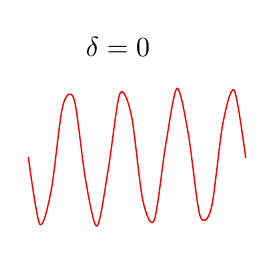
\begin{tikzpicture}
  \begin{scope}[draw=black,line join=round, miter limit=4.00,line width=0.5pt,y=1pt,x=1pt] 
    \XYcross;
  \end{scope}
  
  \begin{scope}[domain=0:3.1415, line join=round, miter limit=4.00,line width=0.5pt, 
                x=25pt,y=25pt, xshift=0, yshift=0]    
    \node at(1.9,1.6) [left, fill=white] {$\delta=0$}; %                         
    \draw[color=red] plot[id=myfce, samples=20, smooth] (\x, {sin(30*\x r)}); % 
  \end{scope}  
\end{tikzpicture}}                              \\
        \end{tabular}
        \caption{a) Modulové charakteristiky paralelního rezonančního obvodu pro napěťový přenos.
                 b) model paralelního rezonančního obvodu a jeho napájení ze zdroje o proměnném 
                 kmitočtu, c) přeměna rezonančního obvodu v oscilátor, d) časová závislost napětí 
                 na svorkách ztrátového LC obvodu po rozkmitání, d) výstupní napětí bezeztrátového 
                 LC obvodu 
                 \cite[s.~135]{Dolecek2009}.}
        \label{AES:fig_MUE6_311}
      \end{figure}
      
      Na obr. \ref{AES:fig_MUE6_311c} je nakreslen paralelní rezonanční obvod, u kterého do obvodu 
      po přepnutí spínače z polohy \(1\) do polohy \(2\) připojujeme předem nabitý kondenzátor. V 
      obvodu vzniknou vlastní tlumené kmity o kmitočtu \(\omega_0\). Obvod lze popsat diferenciální 
      rovnicí
      \begin{equation}\label{AES:eq_osc04}
        \dder{i}{t} + \frac{R}{L}\cdot\der{i}{t} + \omega^2 i = 0
      \end{equation}
      Rovnice má řešení
      \begin{equation}
        i(t) = I_{0}e^{-\delta t}\sin\omega_v t  \qquad u(t) = U_{0}e^{-\delta t}\cos\omega_v t
      \end{equation}
      kde \(I_0\) je \emph{počáteční amplituda proudu}, \(U_0\) je \emph{počáteční amplituda napětí 
      na kapacitoru}, \(\delta = \frac{R}{2L}\) je \textbf{činitel tlumeni obvodu}, \(\omega_0 
      =\frac{1}{\sqrt{LC}}\) je \textbf{rezonanční kmitočet} a \(\omega_v = \sqrt{\omega^2_0 - 
      \delta^2}\) je \textbf{vlastní kmitočet volných kmitů} obvodu. 
      
      Ze vztahu (\ref{AES:eq_osc04}) je zřejmé, Že je-li činitel tlumeni a \textbf{kladný} je 
      kmitání \textbf{tlumené}, je-li a \textbf{záporný} je kmitání \textbf{netlumené}, je-li 
      \(\delta = 0\) mají kmity konstantní amplitudu. Velikost činitele tlumení je závislá na 
      velikosti rezistoru \(R\), který modeluje ztráty v rezonančním obvodu viz obr. 
      \ref{AES:fig_MUE6_311d}, \ref{AES:fig_MUE6_311e}.
      
      V reálném obvodu je vždy \(\delta > 0\) a proto pozorujeme tlumené kmity, jejichž amplituda 
      klesá exponenciálně podle vztahu 
      \begin{equation}\label{AES:eq_osc02}
        u(t) = U_{ss}e^{-\delta t},
      \end{equation}
      kde \(u(t)\) představuje časovou závislost amplitudy kmitů na svorkách paralelního LC obvodu. 
      Dosáhnout nulového tlumení je možné sériovým zapojením rezistoru \(-R_N = R\) - tedy 
      rezistoru se \textbf{záporným odporem}. K tomu by bylo zapotřebí najít takovou součástku, 
      jejíž voltampérová charakteristika vykazuje úsek se zápornou derivací. Hledáme tedy součástky 
      které mají voltampérovou charakteristiku jako je na obr. \ref{AES:fig_AES62a} nebo 
      \ref{AES:fig_AES62b}.
      
      \begin{figure}[ht!]
        \centering  
        \begin{tabular}{cc}
          \subfloat[nelinearita typu \textbf{S}]{\label{AES:fig_AES62a}
            %\documentclass{article}
%\url{http://tex.stackexchange.com/q/82308/86}
%\usepackage{tikz}

\def\xmin{20}
\def\xmax{220}
\def\ymin{-5}
\def\ymax{+220}
\def\zero{0}
\def\phase{25bp}
\def\xlabel{$u$}
\def\ylabel{$i$}

\def\curveS{%
\pgfpathmoveto {\pgfqpoint{25bp}{0bp}} 
\pgfpathcurveto{\pgfqpoint{25bp}{0bp}}
               {\pgfqpoint{104bp}{51bp}}
               {\pgfqpoint{104bp}{69bp}}
\pgfpathcurveto{\pgfqpoint{104bp}{83bp}}
               {\pgfqpoint{72bp}{84bp}}
               {\pgfqpoint{85bp}{101bp}}
\pgfpathcurveto{\pgfqpoint{97bp}{116bp}}
               {\pgfqpoint{176bp}{198bp}}
               {\pgfqpoint{176bp}{198bp}}  
\pgfusepath{stroke}} 

\def\curveN{%
\pgfpathmoveto {\pgfqpoint{25bp}{0bp}}  
\pgfpathcurveto{\pgfqpoint{25bp}{0bp}} 
               {\pgfqpoint{35bp}{65bp}} 
               {\pgfqpoint{53bp}{74bp}}
\pgfpathcurveto{\pgfqpoint{74bp}{83bp}}  
               {\pgfqpoint{89bp}{44bp}}
               {\pgfqpoint{121bp}{59bp}}
\pgfpathcurveto{\pgfqpoint{153bp}{73bp}} 
               {\pgfqpoint{176bp}{198bp}}
               {\pgfqpoint{176bp}{198bp}}  
\pgfusepath{stroke}} 


%\begin{document}

\begin{tikzpicture}[scale=0.3]
  \begin{scope}[draw=black,line join=round, miter limit=4.00,line width=0.5pt,y=1pt,x=1pt] 
    \curveS;
%   \curveN;
    \XYcross;
  \end{scope}  
\end{tikzpicture}

%\end{document}
}                              &
          \subfloat[nelinearita typu \textbf{N}]{\label{AES:fig_AES62b}
            \input{../src/AES/img/AES_62b.tex}}                              
        \end{tabular}
        \caption{Voltampérové charakteristiky s úseky vykazující záporný diferenciální odpor 
        \cite[s.~93]{Koucky1997}}
        \label{MIT:fig_AES_62}
      \end{figure}
      
      Pro sériový model kmitavého obvodu obr. \ref{AES:fig_AES63a} je použitelná nelinearita 
      \texttt{typu S} (např. lavinová dioda), pro paralelní model kmitavého obvodu obr. 
      \ref{AES:fig_AES63b} je použitelná nelinearita \texttt{typu N} (např. tunelová dioda) 
      \cite[s.~93]{Koucky1997}.

      \begin{figure}[ht!]
        \centering  
        \begin{tabular}{cc}
          \subfloat[sériový rezonanční obvod]{\label{AES:fig_AES63a}
            \documentclass{standalone}
    \usepackage{xltxtra}
    \usepackage{tikz}
    \usetikzlibrary{intersections, calc}
    \usepackage[
        american, 
        europeanresistors,
        cuteinductors,  
        smartlabels]{circuitikz}
        \usetikzlibrary{shapes} 
        \ctikzset{bipoles/thickness=1}
        \ctikzset{bipoles/length=0.8cm}
        \ctikzset{bipoles/vsourceam/height/.initial=.7}
        \ctikzset{bipoles/vsourceam/width/.initial=.7}
        \tikzstyle{every node}=[font=\small]
        \tikzstyle{every path}=[line width=0.8pt,line cap=round,line join=round]
\begin{document}
    \begin{circuitikz}
        \draw
        (0,0)
            to[L, l^=$L$] ++(0,2)
            to[short] (2,2)
            to[C, l=$C$] ++(0,-2)
            to [R, l_=$R_N$] ++ (-1,0)
            to [R, l_=$R$] ++ (-1,0) 
            --(0,0);
    \end{circuitikz}
\end{document}    }                              &
          \subfloat[paralelní rezonanční obvod]{\label{AES:fig_AES63b}
            \documentclass{standalone}
    \usepackage{xltxtra}
    \usepackage{tikz}
    \usetikzlibrary{intersections, calc}
    \usepackage[
        american, 
        europeanresistors,
        cuteinductors,  
        smartlabels]{circuitikz}
        \usetikzlibrary{shapes} 
        \ctikzset{bipoles/thickness=1}
        \ctikzset{bipoles/length=0.8cm}
        \ctikzset{bipoles/vsourceam/height/.initial=.7}
        \ctikzset{bipoles/vsourceam/width/.initial=.7}
        \tikzstyle{every node}=[font=\small]
        \tikzstyle{every path}=[line width=0.8pt,line cap=round,line join=round]
\begin{document}
    \begin{circuitikz}
        \draw (0,0)
            to[L, l^=$L$] ++(0,2)
            to[short] ++(3,0) to [R, l=$R_N$] ++ (0,-2) --(0,0);    
        \draw (1,2) to[C, l=$C$,*-*] ++(0,-2);
        \draw (2,2) to [R, l=$R$,*-*] ++ (0,-2);
    \end{circuitikz}
\end{document}}                              
        \end{tabular}
        \caption{ }
        \label{MIT:fig_AES_63}
      \end{figure}
      
      Na velikosti ztrátového odporu \(R\) závisí velikost činitele tlumení \emph{(damping factor)} 
      obvodu podle vztahu:
      \begin{equation}\label{AES:eq_osc01}
        \delta = \frac{R}{2L} \qquad [rad/s]
      \end{equation}
      
      LC oscilátory obsahují klasický rezonanční obvod, jehož rezonanční kmitočet je určen 
      \textbf{Thomsonovým vztahem}:
      \begin{equation}\label{AES:eq_osc03}
        f_0 = \frac{1}{2\pi\cdot\sqrt{LC}} \quad [Hz], \;\text{nebo}\; 
        \omega_0 = \frac{1}{\sqrt{LC}} \quad [rad/s].
      \end{equation}
      
} % tikzset
%---------------------------------------------------------------------------------------------------
\printbibliography[title={Seznam literatury}, heading=subbibliography]
\addcontentsline{toc}{section}{Seznam literatury}
  % !TeX spellcheck = cs_CZ
{\tikzset{external/prefix={tikz/AES/}}
 \tikzset{external/figure name/.add={ch04_}{}}
%---------------------------------------------------------------------------------------------------
% file opamp.tex
%---------------------------------------------------------------------------------------------------
%================================ Kapitola: Zesilovače==============================================
\chapter{Operační zesilovače}
\minitoc
  \section{Úvod}
    \emph{Operační zesilovače} (\texttt{OZ}, aj: \texttt{opamp}) původně vznikly jako složité 
    elektronické obvody pro náročné použití při zpracování analogových (spojitě se měnících) 
    stejnosměrných a nízkofrekvenčních střídavých signálů v analogových počítačích. Moderní 
    polovodičová technologie umožnila vytvoření \texttt{OZ} v podobě levných integrovaných obvodů s 
    malým počtem vývodů, které mají nepatrnou spotřebu, jsou odolné proti přetížení a umožňují 
    jednoduše realizovat nejrůznější elektronická zařízení.
  
    Svůj název získaly z dob \emph{analogových počítačů}, ve kterých se používaly k realizaci 
    matematických operací. Tyto integrované obvody se svými vlastnostmi blíží \emph{ideálním 
    zesilovačům napětí}. Jejich zesílení bez vnější zpětné vazby se blíží nekonečnu ($10^7$). 
    Vstupní odpor je velmi velký ($10^4 \Omega$) a výstupní odpor je malý ($10 \Omega$). Kmitočtový 
    rozsah sahá od stejnosměrného signálu do desítek megahertzů. Vlastní šum a zkreslení zesilovače 
    jsou rovněž malé. V dnešním pojetí je možné vymezit operační zesilovač jako 
    \textbf{stejnosměrný zesilovač} s velkým zesílením a malým vlastním rušením, schopný stabilní 
    činnosti v uzavřené zpětnovazební smyčce \cite[s.~5]{Dostal}.

    Směr signálového toku operačním zesilovačem (dále je OZ) od vstupu k výstupu je vyznačen 
    trojúhelníkovým tvarem jeho symbolické značky na obr. \ref{AES:OP_znacka}.
    \begin{figure}[ht!]
      \centering
      \includegraphics[width=\linewidth]{Dosta_OP_znacka.pdf}
      \caption[Symbolická značka OP]{Symbolická značka OP s vyznačenými signálovými svorkami (a) 
               a skutečná realizace zemní svorky (b, c)}
      \label{AES:OP_znacka}
    \end{figure}
  
    \textbf{Shrnutí}
    \begin{enumerate}\addtolength{\itemsep}{-0.5\baselineskip}
      \item Operační zesilovač má čtyři signálové svorky, i když se často kreslí jen tři - oba 
            vstupy a výstup. Čtvrtou signálovou svorkou je zem.
      \item Souhlasné napětí $u_{CM}$ je totožné s napětím jeho neinvertujícího vstupu $u^+$.
      \item Ideální operační zesilovač má za všech okolností nulové diferenční vstupní napětí a  
            nulové vstupní proudy.
    \end{enumerate}
  
  \section{Parametry operačního zesilovače}
    Ideální operační zesilovač je nedosažitelná abstrakce. K posouzení kvality sku\-teč\-ného 
    operačního zesilovače slouží řada funkčních parametrů jako soubor dat, která lze zjistit 
    měřením na svorkách.
   
    Operační zesilovač, jako každý aktivní elektronický obvod, je obvod nelineární. Funkční 
    charakteristiky OZ však připouštějí linearizaci bez přílišného odklonu od skutečnosti. 
    Odpovídající kvazilineární parametry jsou podkladem lineárního modelu OZ. Ostatní parametry 
    jsou podstatné nelinearity, které tvoří meze jeho lineární oblasti.
    
    \subsection{Lineární parametry a lineární model}
      Obr. \ref{AES:fig_lin_model_opamp} ukazuje úplný \emph{lineární} model operačního zesilovače. 
      Se zřetelem k pozdější analýze chyb operačního obvodu je vhodné rozdělit znázorněné lineární 
      parametry na \textbf{aditivní} a \textbf{multiplikativní}.
      \begin{itemize}\addtolength{\itemsep}{-0.5\baselineskip}
        \item Aditivní parametry zahrnují náhradní rušivé zdroje náhodných fluktuací: $E_R$, 
              $I_R^-$, $I_R^+$, které způsobují aditivní chyby operačního obvodu nezávislé na jeho 
               signálovém vybuzení.
        \item Multiplikativní parametry představované čtyřmi odpory $R_D, R^-_{CM}, R^+_{CM}$,  
              $R_0$ a dvěma řídicími konstantami $-A, 1/X$ závislých generátorů, vystihují pasivní 
              a přenosové vlastnosti OZ způsobují multiplikativní chyby operačních obvodu úměrné 
              jeho signálovému vybuzení.
      \end{itemize}
      Vnitřní, na svorkách neměřitelný napěťový úbytek $e_D$ na odporu $R_D$ zastává v tomto modelu 
      vazbu mezi vstupem a výstupem.
     
      Při práci s proměnnými signály v časové nebo frekvenční oblasti se  význam použitých symbolů 
      vhodně rozšíří na impedance, operátorové přenosy apod.
      \begin{figure}[ht!]
        \centering
        \includegraphics[width=\linewidth]{Dostal_Opamp_model.pdf}
        \caption[Lineární model operačního zesilovače]{Lineární model operačního zesilovače}
        \label{AES:fig_lin_model_opamp}
      \end{figure}
  
    \subsection{Nelineární parametry}
      Chyby, které provázejí aproximaci skutečného operačního zesilovače lineár\-ním modelem, se 
      zvětšují se vstupním a výstupním vybuzením. To se týká zejména linearizace převodní 
      charakteristiky naprázdno $u_0(u_D)$ výrazem $-A(u_D-E_R-e_{CM})$, výstupní charakteristiky 
      $u_0(i_0)$ výrazem $e_0-R_0i_0$ a vstupní charakteristiky $e_{CM}(u_{CM})$ výrazem 
      $u_{CM}/X$.  Skutečný průběh každé z těchto charakteristik se vyznačuje velmi ostrým kolenem, 
      při jehož překročení ztrácejí lineární parametry smysl.  Signálové vybuzení, které přísluší 
      tomuto kolenu, tak vymezuje dosti přesně oblast lineárního chování \cite[s.~29]{Dostal}.
  
      Třem svorkovým proměnným $u_{CM}, u_O, i_0$ přísluší tři \emph{statické nelinearity} (omezení 
      rozkmitu) a tři dynamické nelinearity (omezení rychlosti)
  
  \section{Ideální operační obvod}
    \subsection{Paralelní operační obvod}
      \fbox{Napěťový invertor} ukazuje, že vstupní signálový proud může být generován také 
      synteticky, kombinací napěťového signálového zdroje a sériového rezistoru. Takovým způsobem 
      vytvořený \emph{napěťový invertor} na obr. * je jedním z nejčastějších operačních obvodů. 
      
      Vstupní napětí $u_s$ je celé vloženo na rezistor $R_1$ (jeho pravý konec je virtuálně 
      uzemněn) a vyvolává ekvivalentní vstupní proud $\frac{u_s}{R_1}$. Tento přitékající proud je 
      kompenzován proudem $-\frac{u_0}{R_2}$ odsávaným přes zpětnovazební rezistor $R_2$ do výstupu 
      operačního zesilovače $$\frac{u_s}{R_1}=-\frac{u_0}{R_2}.$$ Ideální operační rovnice
      \begin{equation}\label{AES:eq_opamp_inv02}
        u_0 = - \frac{R_2}{R_1}u_s.
      \end{equation}
      Vyjadřuje úměrnost signálových napětí $-u_0$ a $u_s$ velikostem přilehlých rezistorů $R_2$ a 
      $R_1$. Pro snadnější zapamatování se nabízí představa dvouramenné páky s délkami ramen $R_1$ 
      a $R_2$, otočné v bodě odpovídajícímu virtuální zemi, která přenáší výchylku $u_s$ levého 
      konce na výchylku $u_0$ pravého konce v opačné polaritě.

      \begin{figure}[ht!]
        \centering
        \begin{tabular}{c}
          \subfloat[$u_0 = -\dfrac{R_2}{R_1}u_s, \qquad R_{||} = R_1, \qquad R_{\mathsf{O}|} = 
          0$]{\label{{ES:fig_004a}}
            \includegraphics[width=0.5\linewidth]{opamp_inv01a.pdf}}             \\
          \subfloat[ $u_0 = -\dfrac{R_2}{R_2+R_s}u_s$ ]{\label{AES:fig_004b}
            \includegraphics[width=0.51\linewidth]{opamp_inv01b.pdf}}             
        \end{tabular}
        \caption{Napěťový invertor. Jeho mechanickou analogií je dvouramenná páka (a). Přítomnost 
                 vnitřního odporu signálového zdroje $R_s$ v operační rovnici je důsledkem 
                 konečného vstupního odporu $R_{||} = R_1$ (b). }
        \label{AES:fig_opamp_inv01} 
      \end{figure}
      Zesílení napěťového invertoru 
      \begin{equation}\label{AES:eq_opamp_inv01}
        G_i = -\frac{R_2}{R_1},
      \end{equation} 
      je záporné a nastavitelné v širokých mezích od $0$ do $\infty$ výběrem rezistorů $R_1$ a 
      $R_2$. Zvláštním případem je jednotkový invertor se stejnými rezistory $R_1 = R_2$, který 
      prostě invertuje polaritu vstupního napětí: $$u_0 = - u_s, \qquad G_i = -1.$$
      
      Výstupní odpor napěťového invertoru je ideálně nulový. Jeho vstupní odpor však ztrácí onen 
      vyhranění charakter typický pro kanonické operační obvody a nabývá indiferentní velikosti 
      \begin{equation}\label{AES:eq_opamp_inv03}
        R_{||} = R_1,
      \end{equation} 
      rovné velikosti virtuálně uzemněného rezistoru $R_1$.
      
      Napěťový invertor zatěžuje signálový zdroj (obr. *). To se projevuje poklesem svorkového 
      napětí signálového zdroje o úbytek na vnitřním odporu $R_s$, nebo jinak řečeno, přítomností 
      nedefinovaného a nestálého vnitřního odporu $R_s$ v operační rovnici invertoru:  
      \begin{equation}\label{AES:eq_opamp_inv04}
       u_0 = -\frac{R_2}{R_1 + R_s}u_s.
      \end{equation}      
      Taková vlastnost se obvykle považuje za nedostatek. 
            
    \subsection{Sériový operační obvod}
    
    \subsection{Složený operační obvod}
      Operační obvody, které není možné zahrnout do předcházejích dvou velkých tříd, se vyznačují:
        \begin{itemize}\addtolength{\itemsep}{-0.5\baselineskip}
          \item signálovým buzením obou vstupů operačního zesilovače,
          \item násobnou zpětnou vazbou,
          \item kombinací záporné a kladné zpětné vazby,
          \item použitím několika operačních zesilovačů,
          \item nestandardním zapojením operačního zesilovače.
        \end{itemize}
      \subsubsection{Signálové buzení obou vstupů}
        \fbox{Rozdílový zesilovač} na obr. \ref{AES:fig_diff_opamp01} je lineární operační obvod se dvěma vstupy. Jeho výstupní napětí se najde superpozicí \cite[s.~126]{Dostal}. 
        
        Nechť působí napětí $u_1$ a napětí $u_2$ je nulové. Neinvertující vstup operačního 
        zesilovače je uzemněn přes paralelní kombinaci rezistorů $R_3$ a $R_4$. Operační obvod 
        představuje napěťový invertor a první složka výstupního napětí má velikost 
        $$-\frac{R_2}{R_1}u_1.$$
        
        Nechť působí napětí $u_2$ a napětí $u_1$ je nulové. Operační obvod představuje neinvertujcí 
        zesilovač s předřazeným děličem $R_3$ a $R_4$ a druhá složka výstupního napětí má velikost 
        $$u_2\frac{R_4}{R_3+R_4}\left(\frac{R_2}{R_1}+1\right)= 
        u_2\frac{R_2/R_1+1}{R_4/R_3+1}\cdot\frac{R_4}{R_3}.$$
        
        %----------------------------------
        % image: rozdílový zesilovač
        % !TeX spellcheck = cs_CZ
% Diferenciální zesilovač
% pozn: symbol země (ground) je předefinován v knihovně wiking.sty

% Define box and box title style
% http://www.texample.net/tikz/examples/boxes-with-text-and-math/
\tikzstyle{mybox} = [draw=red, fill=blue!20, very thick,
    rectangle, rounded corners, inner sep=5pt, inner ysep=10pt, inner xsep=10pt ]
\tikzstyle{fancytitle} =[fill=red, text=white]

\begin{figure*}[ht!]
  \centering
  \begin{circuitikz}[scale=1, every node/.style={scale=1}]
    \ctikzset{resistor=european}
%    \ctikzset{tripoles/op amp/scale=0.5}
    \draw (0,0) node[op amp, scale=0.5] (opamp) {};
    \node [left=0.1cm of opamp.-]       (p1) {};
    \node [left=0.1cm of opamp.+]       (p2) {};
    \node [above=0.5cm of p1]           (A)  {};
    \node [left=1.5cm of A]             (p3) {};
    \node [right=1.5cm of A, coordinate](C)  {};
    \node [right=0.5cm of C]            (p6) {};
    \node [below=0.5cm of p2]           (B)  {};
    \node [left=1.5cm of B]             (p4) {};
    \node [right=1.5cm of B]        (ground) {};
    \node [right=0.1cm of opamp.out, coordinate] (vo) {};
    %%% Draw connections
    \draw (p3) node[left] {$u_1$} to[R=$R_1$,o-] (A)  to[R=$R_2$,*-] (C); 
    \draw (opamp.-)   to[short] (p1) to[short] (A);
    \draw (opamp.out) to[short] (vo);
    \draw (vo) to[short,-*] (vo |- C); 
    \draw (p4) node[left] {$u_2$} to[R=$R_3$,o-] (B)  to[R=$R_4$,*-] (ground) node [sground] {};  
    \draw (opamp.+) to[short] (p2) to[short] (B); 
    \draw (C) to[short,-o] (p6) node[right] {$u_{0}$};
    \node[above] at (A) {A}; % text 
    \node[below] at (B) {B}; % text 
    %%% minipage
    \node [mybox, right=5cm of p2] (box){%
       \begin{minipage}[l]{3cm}
          \begin{align*}
              \frac{R_4}{R_3} &= \frac{R_2}{R_1} \\
              u_0             &= \frac{R_2}{R_1}(u_2 - u_1) \\
              R_{|1|}         &= R_1 \\
              R_{|2|}         &= R_3 + R_4 \\
              R_{\mathsf{O}|} &= 0
          \end{align*}
       \end{minipage}
    };
    \node[fancytitle, right=10pt, rounded corners] at (box.north west) {rovnice:};
   %\node[fancytitle, rounded corners] at (box.east) {$\clubsuit$};
    %%% text R_{|1|} and R_{|2|}
    \draw[->] (-4.0,0.2) -- +(0,0.5) node[left] {$R_{|1|}$} -- +(0.5,0.5);
    \draw[->] (-4.0,-0.2) -- +(0,-0.5) node[left] {$R_{|2|}$} -- +(0.5,-0.5);
  \end{circuitikz} 
  \caption{Rozdílový zesilovač. Podmínky potlačení souhlasné složky vstupních napětí $u_1$ a 
           $u_2$ je poměrové vyvážení zpětnovazebních rezistorů, $R_4/R_3 = R_2/R_1$. S ohledem na 
           ofset se obvykle volí uplná symetrie, tj. $R_4 = R_2$ a $R_3 = R_1$.}
  \label{AES:fig_diff_opamp01}         
\end{figure*} 
        %---------------------------------- 
               
        Současné působení obou vstupních napětí ve vyváženém operačním obvodě $$\frac{R_4}{R_3}=\frac{R_2}{R_1},$$ přísluší výstupní napětí 
        \begin{equation}\label{AES:eq_diff_opamp}
          u_2 = \frac{R_2}{R_1}(u_2-u_1),   
        \end{equation}
        úměrné rozdílu vstupních napětí bez ohledu na jejich absolutní velikost. Odtud název 
        operačního obvodu. Důvod zařazení napěťového děliče ($R_3$,$R_4$) je zřejmý - dělič 
        sjednocuje zesílení invertujícího a neinvertujícího vstupu, která se liší absolutně o 
        jednotku. 
        
        Dvěma vstupům přísluší dva vstupní odpory. První vstupní odpor $$R_{|1|} = R_1$$ je roven 
        velikosti rezistoru $R_1$, protože vnitřní odpor bodu $A$\footnote{obdoba virtuální země} 
        je nulový. Druhý vstupní odpor $$R_{|2|} = R_3 + R_4$$ je roven součtu rezistorů $R_3$ a 
        $R_4$, protože vnitřní odpor zbytku operačního obvodu v bodě $B$ je nekonečný. Tyto dva 
        vstupní odpory jsou různé, i když jsou obě větve ($R_1$, $R_2$) a ($R_3$, $R_4$) stejné. 
        
        Vstupní odpory $R_{|1|}$ a $R_{|2|}$ přísluší dvěma samostatným uzemněným zdrojům 
        signálových napětí $u_1$ a $u_2$ podle \ref{AES:fig_diff_opamp01}. Volnému (izolovanému) 
        signálovému napěťovému zdroji připojenému diferenčně mezi vstupy rozdílového zesilovače, by 
        příslušel diferenční vstupní odpor $$R_{|D|} = R_1 + R_3,$$ rovný součtové velikosti 
        rezistorů $R_{|1|}$ a $R_{|3|}$, protože body $A$ a $B$ jsou virtuálně zkratovány.

} % tikzset
%---------------------------------------------------------------------------------------------------
\printbibliography[title={Seznam literatury}, heading=subbibliography]
\addcontentsline{toc}{section}{Seznam literatury}
  
  % !TeX spellcheck = cs_CZ
%---------------------------------------------------------------------------------------------------
% file DA_AD_converter.tex
%---------------------------------------------------------------------------------------------------
%======================= Kapitola: Konverze mezi digitálním a analogový signálem====================
\setchaptertoc
\chapter{Konverze mezi digitálním a analogový sig\-ná\-lem}


\section{Konverze mezi digitálním a analogový signálem}
  Při zpracování analogového signálu je jednou z důležitých funkcí převod tohoto signálu z analogové
  podoby do číslicové a naopak. Proto jsou analogově-číslicové převodníky resp. číslicově-analogové
  převodníky (ADC - Analog-to-Digital Converter), (DAC - Digital-to-Analog Converter) velmi
  důležitými prvky jakéhokoli systému zpracovávajícího signál \cite[s.~11]{Haze}. Na obrázku
  \ref{AES:fig_ADC_DAC_IO} je definováno rozhraní obou typů převodníku.
  \begin{figure}[ht!]
     \centering
     \includegraphics[width=\linewidth]{ADC_DAC_block.pdf}
     \caption[Definice I/O bloku DAC a ADC ]{Definice rozhraní bloku analogově-číslicového (ADC) a 
              číslicově-analogového (DAC) převodníku}
     \label{AES:fig_ADC_DAC_IO}
  \end{figure}

  \textbf{Analogově-číslicové převodníky} (Analog-to-Digital Converters) slouží k pře\-ve\-de\-ní 
  analogového signálu na signál číslicový. Pro A/D převodník má analogová stupnice vstupního 
  signálu délku \texttt{FS} (\emph{Full scale}), udávanou např. ve voltech. Stupnice číslicového 
  signálu pak vyznačuje diskrétní hodnoty výstupu, které převodník generuje při převodu analogového 
  signálu \cite[s.~202]{Neumann}.

  \textbf{Číslicově-analogové převodníky} (Digital-to-Analog Converters) slouží k o\-pač\-né\-mu 
  procesu, tedy k pře\-ve\-de\-ní číslicového signálu na signál analogový, což by šlo realizovat 
  pomocí lineárního digitálního potenciometru a připojeného zdroje referenčního napětí na jeho 
  vstupu \cite[s.~208]{Neumann}. Pro N-bitové binární slovo by musel mít $n-1$ rezistorů a $n$ 
  resp. $2n - 1$ spínačů. To je monoliticky téměř nerealizovatelné již pro osmi- a vícebitové 
  slovo. Řešení převodníků proto musí být mnohem úspornější, i když úspory budou vykoupeny jinými 
  nevýhodami, případně omezeními pro jejich použití.

    \subsection{Základní struktura převodníků}
      Obě skupiny převodníků mohou typicky obsahovat komparátory, číslicové obvody, spínače, 
      integrátory, vzorkovací obvody a/nebo pasivní součástky. Nezbytnou a důležitou součástí je i 
      přesný zdroj referenčního napětí. V mnoha případech pak také platí, že DAC je jednou z částí 
      ADC.
      
      Analogově číslicový převod můžeme pomyslně rozložit do tří etap \cite{Sebesta}.
      \begin{enumerate}[noitemsep]
        \item Převod signálu se spojitým časem na signál s diskrétním časem. Tomuto převodu říkáme  
              vzorkování.
        \item Kvantování vzorku s cílem vyjádřit vzorky konečnou množinou čísel. Tento krok je 
              provázen vznikem tzv. kvantovacího šumu. Uvedený jev souvisí s nelineárním zkreslením 
              známým z teorie obvodů.
        \item Kódování spočívající zpravidla v binárním vyjádření čísel představujících velikosti  
              vzorku.
      \end{enumerate}
      
    \subsection{Statické a dynamické parametry převodníků}
      Statické parametry převodníků jsou určovány pomocí \emph{převodní charakteristiky}, zatím co
      dynamické vlastnosti se vyhodnocují z kmitočtového spektra převodníku \cite[s.~11]{Haze}.
      \begin{itemize}[noitemsep]
        \item rozsah,
        \item integrální a diferenciální nelinearita (\emph{integral - INL, differential - DNL nonlinearity}),
        \item rozlišení převodníku (\emph{resolution}),
        \item přesnost (\emph{accuracy}),
        \item chyba monotónnosti,
        \item chyba nastavení nuly (\emph{offset error}),
        \item hystereze a další.
       \end{itemize}
       K hlavním dynamickým parametrům patří
       \begin{itemize}[noitemsep]
         \item odstup signál - šum (\emph{signal to noise ratio - SNR}) kap. \ref{AES:cap_SNR},
         \item efektivní počet bitů (\emph{effective number of bits - ENOB}),
         \item harmonické zkreslení (\emph{total harmonic distortion - THD}),
         \item odstup signál-šum a zkreslení (\emph{signal to noise and distortion - SINAD}),
         \item dynamický rozsah bez parazitních složek \newline(\emph{spurious free dynamic range 
               - SFDR}),
         \item šum - vrcholový, efektivní (\emph{noise - peak, rms}),
         \item doba přepnutí a ustálení.
       \end{itemize}

    \subsection{Vzorkování}
    \subsection{Kvantování}
       Pro přechod od časově spojitého signálu se spojitou množinou hodnot k číslicovému signálu, 
       je nutné provést (výškové) \texttt{kvantování}, tj. kvantování hodnot signálu, které je 
       patrné z obrázku \ref{AES:fig_Quntized_sig_wave}. Je zřejmé, že mapování spojitého intervalu 
       vstupních hodnot na diskrétní hodnoty digitálního výstupu způsobí, že každá hodnota 
       digitálního výstupu platí pro vstupní signál měnící se v určitém  podintervalu. Délka 
       podintervalu, pro který platí jedna hodnota digitálního výstupu se nazývá 
       \textbf{kvantizační krok převodníku} - \emph{Q}, jenž je roven bitu s nejnižší váhou - 
       \texttt{LSB}.

       \begin{figure}[ht!]
         \centering
         \includegraphics[width=1\linewidth]{ADC_DAC_3bit.pdf}
         \caption[Přenosová funkce AD a DA převodníku]{Ideální přenosová funkce 3bitového    
                  unipolárního AD a DA převodníku. V případě DA převodníku je přenosová funkce 
                  tvořena osmi body, nikoliv čárou.}
         \label{AES:fig_3b_DAC_ADC}
       \end{figure}
 
       Převodní charakteristika DA i AD převodníku je znázorněna na obr. \ref{AES:fig_3b_DAC_ADC}. 
       Analogový signál je spojitý a číslicový signál vyjadřuje jen jeho vybrané diskrétní hodnoty. 
       Proto je převodní charakteristika nespojitá. Naproti tomu digitální vstup vytvoří na výstupu 
       pouze omezený počet hodnot výstupního signálu.

       \begin{figure}[ht!]
         \centering
         \includegraphics[width=1\linewidth]{Uni_Bi_Converter.pdf}
         \caption[Unipolární a bipolární převodníky]{Unipolární a bipolární převodníky \cite{Kester2004}}
         \label{AES:fig_uni_bi_converter}
       \end{figure}

       Počet úrovní AD převodníku, do kterého je rozdělen rozsah vstupního analogového signálu 
       definuje \textbf{rozlišovací schopnost ADC} a lze ji vyjádřit různými způsoby, jak ukazuje 
       tabulka \ref{AES:tab_10b_ADC_resolution} pro 2 až 24bitového převodníku.

         \begin{table*}[ht!]
           \centering
            \setlength{\tabcolsep}{5pt}
            \begin{tabular}{|c|c|c|c|c|c|}
              \hline
                \textbf{Rozlišení} & \multirow{2}{*}{$\mathbf{2^N}$} &  \textbf{Napětí} & 
                \multirow{2}{*}{\textbf{ppm FS}}& \multirow{2}{*}{\textbf{\% FS}}&   
                \multirow{2}{*}{\textbf{dB FS}}                                                 \\
                         N     &           &  \textbf{10V FS} &        &             &          \\
              \hline
                       2-bit   &         4 &            2.5 V & 250000 &          25 &  -12     \\
              \hline
                       4-bit   &        16 &           625 mV &  62500 &        6,25 &  -24     \\
              \hline
                       6-bit   &        64 &           156 mV &  15625 &        1,56 &  -36     \\
              \hline
                       8-bit   &       256 &          39,1 mV &   3906 &        0,39 &  -48     \\
              \hline
                      10-bit   &      1024 &          9,77 mV &    977 &       0,098 &  -60     \\
              \hline
                      12-bit   &      4096 &          2.44 mV &    244 &       0,024 &  -72     \\
              \hline
                      14-bit   &     16384 &       610 $\mu$V &     61 &       0,061 &  -84     \\
              \hline
                      16-bit   &     65536 &       153 $\mu$V &     15 &      0,0015 &  -96     \\
              \hline
                      18-bit   &    262144 &         38 $\mu$ &      4 &      0,0004 & -108     \\
              \hline
                      20-bit   &   1048576 &       9.54 $\mu$ &      1 &      0,0001 & -120     \\
              \hline
                      22-bit   &   4194304 &       2.38 $\mu$ &   0,24 &    0,000024 & -132     \\
              \hline
                      24-bit   &  16777216 &           596 nV &   0,06 &    0,000006 & -144     \\
              \hline
           \end{tabular}
           \caption[Kvantizace: Velikost LSB]{Porovnání rozlišovací schopnosti AD převodníku s  
                    různou délkou výstupního slova. Z tabulky vyplývá, že kvantizační krok 
                    24bitového ADC odpovídá velikosti úbytku na rezistoru $2,2 k\Omega$ při teplotě 
                    25°C, který vzniká vlivem tepelného šumu (viz Johnsonův šum) jenž je při šířce 
                    pásma 10 kHz roven 600 nV. }
           \label{AES:tab_10b_ADC_resolution}
         \end{table*}

       \begin{figure}[ht!]
         \centering
         \includegraphics[width=1\linewidth]{Quantized_signal_wave.pdf}
         \caption[Kvantizační chyba]{Kvantizační chyba je rovna rozdílu původního x(t) a kvantovaného signálu v úrovni y(t) \cite{Bennett}}
         \label{AES:fig_Quntized_sig_wave}
       \end{figure}

       %The quantization error for any ac signal which spans more than a few LSBs can be 
       %approximated by an uncorrelated sawtooth waveform having a peak-to-peak amplitude of q, the 
       %weight of an LSB. Although this analysis is not precise, it is accurate enough for 
       %most applications. W. R. Bennett of Bell Laboratories analyzed the actual spectrum of 
       %quantization noise in his classic 1948

       Kvantizační chyba, jejíž průběh je na obr. \ref{AES:fig_Quntized_sig_wave}, v dynamickém 
       režimu, tj. při časových změnách vstupní analogové veličiny, způsobuje \textbf{kvantizační 
       šum}. Ten lze pozorovat např. tehdy, kdy čísla získaná z převodníku A/D jsou vedena do 
       převodníku D/A a jím je analogový signál rekonstruován. Rekonstruovaný signál se jeví jako 
       signál původní, avšak se superponovaným rušivým signálem. Vzájemným odečtení 
       rekonstruovaného a původního signálu, dostaneme samostatný rušivý signál, který lze podrobit 
       analýze. \emph{Pokud je vzorkovací signál nekorelovaný se vzorkovaným signálem, je možno 
       kvantizační šum považovat za náhodný}. Vztah mezi původním signálem a signálem degradovaným 
       kvantizačním šumem vyjadřuje parametr - \texttt{SNR}
       \begin{itemize}
         \item SNR  - Signal to Noise Ratio: poměr signálu k šumu
             \begin{equation}\label{AES:eq_SNR}
                SNR = \frac{E\{x^2(t)\}}{E\{[y(t)-x(t)]^2\}}
             \end{equation}
                \begin{itemize}
                   \item $E\{.\} \cdots$ operátor průměrování
                   \item $x(t)   \cdots$ vstupní analogový signál
                   \item $y(t)   \cdots$ rekonstruovaný kvantovaný signál
                 \end{itemize}
       \end{itemize}
       Kvantizační chybu lze aproximovat nekorelovaným pilovým průběhem s amplitudou špička-špička 
       rovnou kvantizačnímu kroku $Q$. Ačkoliv takto provedená analýza (viz kapitola 
       \ref{AES:kap_kv_sum}) není přesná, v běžných aplikacích zcela postačuje.

       Na obr. \ref{AES:fig_AD_kvantizacni_chyba} je kvantování realizováno tak, že je zajištěna 
       minimální chyba kvantování, tj. převodník provádí operaci zaokrouhlování na nejbližší 
       hodnotu. To znamená, že např. číslo jedna bude generováno vstupem v intervalu $1\pm0,5V$, 
       je-li \texttt{FS} rovno 8V a máme-li k dispozici osm kvantizačních úrovní.

       Převodník, který má v celém intervalu předváděných vstupních hodnot konstantní kvantizační 
       krok, se též označuje jako lineární kvantizér. Převodník s přirozeným binárním kódem o 
       \emph{N} bitech je schopen na analogové straně reprezentovat \emph{n-1} ne\-nu\-lo\-vých 
       úrovní analogové veličiny, přičemž platí
       \begin{equation}\label{AES:eq_AD_kod}
          n = 2^N
       \end{equation}
       A jde-li o lineární N-bitový kvantizér, můžeme vyjádřit kvantizační krok vztahem
       \begin{equation}\label{AES:eq_kvant_krok}
          Q = \frac{FS}{n} = \frac{FS}{2^N}
       \end{equation}
       Nejvyšší úroveň vstupní veličiny \emph{A} pak bude
       \begin{equation}\label{AES:eq_A_max}
          A_{max} = \frac{n-1}{n}+\frac{Q}{2}
       \end{equation}

       V sekvenci bitů binárního čísla generovaného převodníkem se zpravidla první bit, který
       představuje nejvyšší binární řád, označuje \texttt{MSB} (\emph{Most Significant Bit}), tedy
       nejvýznamnější bit. Poslední bit, tj. bit v poloze nejnižšího řádu, má označení \texttt{LSB}
       (\emph{Least Significant Bit}), tedy nejméně významný bit. Je zřejmé, že \texttt{LSB}
       jednoznačně určuje základní krok na ose číslicového signálu. Dojde-li ke změně pouze v
       hodnotě \texttt{LSB}, změní se analogová hodnota právě o kvantizační krok. \texttt{LSB} tedy
       na analogové straně určuje rozlišovací schopnost převodníku. Např. osmibitový převodník má
       rozlišovací schopnost \texttt{FS/256}, tj. přibližně \texttt{0,4\%}. Je-li \texttt{FS = 2V},
       musí rozlišit \texttt{8 mV}\cite[s.~203]{Neumann}.

       Vzhledem k diskretizaci hodnot původního analogového signálu při převodu A/D dochází ke
       \emph{kvantizačním chybám}. Je-li např. vstupní veličinou okamžité napětí $u_a$ a této
       hodnotě odpovídá na výstupu číslo $D$, pak kvantizační chybu $\varepsilon_q$ lze vyjádřit
       takto:
       \begin{equation}\label{AES:eq_kvant_chyba}
          \varepsilon_q = u_a - FS\frac{D}{2^N}
       \end{equation}

      \subsection{Kvantizační šum ideálního N-bitového ADC}\label{AES:kap_kv_sum}

      %The only errors (dc or ac) associated with an ideal N-bit data converter are those related  
      %to the sampling and quantization processes. The maximum error an ideal converter makes when 
      %digitizing a signal is $\pm 1/2 LSB$. The transfer function of an ideal N-bit ADC is shown 
      %in Figure 2.37. The quantization error for any ac signal which spans more than a few LSBs 
      %can be approximated by an uncorrelated sawtooth waveform having a peak-to-peak amplitude of 
      %q, the weight of an LSB.

      %The quantization error for any ac signal which spans more than a few LSBs can be 
      %approximated by an uncorrelated sawtooth waveform having a peak-to-peak amplitude of q, the 
      %weight of an LSB. Although this analysis is not precise, it is accurate enough for most 
      %applications. W. R. Bennett of Bell Laboratories analyzed the actual spectrum of 
      %quantization noise in his classic 1948

      V předchozí kapitole byla nastíněna možnost aproximace kvantizační chyby jaké\-ho\-koliv AC 
      signálu v časové oblasti (viz \ref{AES:fig_Quntized_sig_wave}) nekorelovaným pilovým 
      průběhem, za cenu určité nepřesnosti vyvážené jednodušším matematickým aparátem.

      Vyjděme tedy z převodní charakteristiky ideálního N-bitového převodníku zatížené kvantizační 
      chybou, tak jak je znázorněna na obr. \ref{AES:fig_AD_kvantizacni_chyba}. Z té je patrné, že 
      chyba může v absolutní hodnotě dosáhnout maximálně $e(t) = \frac{Q}{2}$, resp. 
      $\pm\frac{1}{2}LSB$ a v rámci kvantizačním kroku ji lze popsat přímkou se strmostí 
      \texttt{s}: $$e(t) = st, -\frac{Q}{2s}<t<+\frac{Q}{2s}.$$ Statisticky je pravděpodobnost 
      jejího rozložení 1/Q a je rovnoměrná od $-\frac{Q}{2}$ do $+\frac{Q}{2}$.

      \begin{figure}[ht!]
        \centering
        \includegraphics[width=0.8\linewidth]{AD_kvantizacni_chyba.pdf}
        \caption[Převodní charakteristika ideálních převodníků]{Převodní charakteristika 
                 ideálních převodníků a závislost chyby kvantizace na vstupní analogové hodnotě}
        \label{AES:fig_AD_kvantizacni_chyba}
      \end{figure}

      Z výše uvedeného plyne, že okamžitá hodnota kvantizační chyby $\varepsilon_q(t) = y(t) - x(t)$
      může dosáhnout rozkmitu maximálně $\pm \frac{Q}{2}$ a jelikož předpokládáme rovnoměrné
      rozložení hodnot, je hustota pravděpodobnosti amplitud rovna $\frac{1}{Q}$.

      \emph{Kvantizační šum $\sigma^2$ je definován jako výkon (rozptyl) střídavé složky kvantizační
      chyby $\varepsilon_q$ a jeho efektivní hodnotu $\sigma$ můžeme odvodit pomocí věty o druhém
      centrálním momentu nebo výpočtem efektivní hodnoty v časové oblasti.}

        \begin{figure}[ht!]
          \centering
          \subcaptionbox{Hustota pravděpodobnosti kvantizačního šumu \label{AES:fig_kvant_sum1}}
            {\luafigure[0.45]{AD_kvantizacni_sum1.pdf}}
          \subcaptionbox{Kvantizační šum jako funkce času \label{AES:fig_kvant_sum2}}
            {\luafigure[0.45]{AD_kvantizacni_sum2.pdf}}
          \caption{K odvození efektivní hodnoty kvantizačního šumu}
          \label{AES:fig_kvant_sum}
        \end{figure}

        \begin{enumerate}[noitemsep]
          \item V pravděpodobnostním počtu je K-tý moment definován jako: 
                \begin{align*}
                  M_k  &= \int_{-\infty}^{\infty} x^k p(x)dx                           \\
                  \shortintertext{tedy}                      
                  e(t) &= \int_{-\frac{Q}{2}}^{+\frac{Q}{2}}(x - x_0)^2p(x)dx = 
                                 \frac{1}{Q}\int_{-\frac{Q}{2}}^{+\frac{Q}{2}}x^2dx    \\
                       &= \frac{Q^2}{12}
                \end{align*}
          \item V časové oblasti má kvantizační šum pilový průběh viz obr.    
                \ref{AES:fig_kvant_sum2}. Z  definičního integrálu efektivní hodnoty dostaneme $$ 
                \overline{e^2(t)} =               
                \frac{s}{Q}\int_{-\frac{Q}{2}}^{+\frac{Q}{2}}(st)^2dt = \frac{Q^2}{12}.$$ Též 
                můžeme využít znalosti efektivní hodnoty pro průběh tohoto typu: 
                $\frac{U_m}{\sqrt{3}}$ a dosazením za $U_m =\frac{Q}{2}$ získáme opět stejný 
                výsledek jako při výpočtu integrálu
        \end{enumerate}

        Tedy efektivní hodnota kvantizačního šumu ideálního N-bitového převodníku je:
        \begin{equation}\label{AES:eq_ef_kv_sumu}
            e(t) = \frac{Q}{\sqrt{12}}
        \end{equation}
        Předpokládejme na vstupu převodníku ustálený harmonický signál o amplitudě $X$. Dále 
        předpokládejme, že signál s amplitudou $X_m$ by pokryl celý rozsah převodníku $FS$. Pak se 
        dá ze vztahu \ref{AES:eq_SNR} vyjádřit odstup signálu od šumu \texttt{SNR} ideálního 
        \emph{N-bitového} převodníku jako podíl jejich výkonů resp. kvadrátu efektivních hodnot 
        signálu a šumu v decibelech vztahem
        \begin{align*}
          SNR      &= \frac{P_{signal}}{P_{noise}} =     
                      \left(\frac{A_{signal}}{A_{noise}}\right)^2         \\
          SNR_{dB} &= 10\log\frac{P_{signal}}{P_{noise}} =       
                      10\log\left(\frac{A_{signal}}{A_{noise}}\right)^2   \\
                   &= 20\log\frac{A_{signal}}{A_{noise}}                  
        \end{align*}
        \begin{equation}\label{AES:eq_SNR_N}
            SNR  = 1,76 + 6,02N + 20log\left(\frac{X}{X_m}\right)
        \end{equation}

        Lze tedy říci, že každý bit navíc v digitálním výstupu A/D převodníku přinese zlepšení 
        odstupu signálu od šumu o \texttt{6 dB}. Naproti tomu je třeba vědět, že uvedený výraz 
        počítá s harmonickým signálem různého rozkmitu. Při zmenšování amplitudy bude relativní 
        podíl šumu v signálu vyšší. Poměry se také mohou velmi změnit, když signál nebude mít 
        harmonický charakter.

      \subsubsection{Odstup signálu od šumu}\label{AES:cap_SNR}
        Z předchozí kapitoly víme, že SNR je definován jako poměr výkonu signálu k výkonu šumu
        ($v\acute{y}kon = ef. hodnota^2$). Pro samotný kvantizační šum platí:
        \begin{align}
          SNR_{dB} &= 10\log\left(\frac{\dfrac{2^N}{2\cdot\sqrt{2}}\cdot     
                                        Q}{\dfrac{Q}{\sqrt{12}}}\right)^2          \nonumber \\
                   &= N20\log2 + 20\log\frac{\sqrt{12}}{2\cdot\sqrt{12}}           \nonumber \\ 
          SNR_{dB} &= 6,02\cdot N + 1,76dB
        \end{align}

        \begin{figure}[ht!]
            \centering
            \includegraphics[width=0.6\linewidth]{AD_SNR.pdf}
            \caption{}
            \label{AES:fig_SNR}
        \end{figure}

        Tato hodnota platí pouze pro ideální převodník pouze s kvantizační chybou, a sinusový 
        signál s rozkmitem přes celý rozsah převodníku.  Skutečný převodník má ovšem vlivem dalších 
        chyb \texttt{SNR} menší než \texttt{SNR} určený pouze pro kvantizační šum. Tato hodnota se 
        nazývá \texttt{SINAD} nebo \texttt{SNDR} - \emph{Signal-to-Noise and Distortion ratio}.

        Známe-li \texttt{SNR} skutečného převodníku, můžeme určit počet efektivních bitu $N_{ef}$ 
        tzn. \emph{efektivní rozlišitelnost převodníku}. Ten je vždy menší než $N$.
        \begin{equation}\label{AES_eq_N_ef}
            N_{ef} = \frac{SNR - 1,76}{6,02}
        \end{equation}
        
  \section{Principy A/D převodníků}
      Převod analogového signálu na číslo lze uskutečnit několika různými postupy:\cite{Neumann}
      \begin{enumerate}[noitemsep]
        \item Vstupní signál se porovnává s kvantovanou referenční veličinou a komparátory okamžitě 
              vyhodnotí, který z nich je větší. Přímým výstupním údajem je binární číslicové slovo.
        \item Vstupní signál i referenční veličina se v určité časové sekvenci zavádějí do   
              integrátoru a komparátor na jeho výstupu určuje sekvenci impulsů, vypovídající o 
              hodnotě vstupní analogové veličiny. Informací o vstupní veličině dále přenáší počet 
              impulsu, jejich kmitočet nebo kódovaná sekvence impulsů. Tato informace může být 
              převedena číslicovým blokem (obvykle blokem DSP) na binární číslicové slovo.
      \end{enumerate}

      Bývá také používáno třídění na \emph{převodníky s přímým a nepřímým vyhodnocení analogové 
      veličiny}.
      \begin{itemize}
        \item \texttt{Převodníky s přímým vyhodnocením} porovnávají hodnoty analogové veličiny s  
              vybranými kvantizačními úrovněmi současně nebo postupně, a to tak, že každá úroveň má 
              vlastní komparátor. K těmto převodníkům patří \emph{převodníky paralelní a kaskádní}.
        \item \texttt{K nepřímému převodu} můžeme využít postupného provoláváním vstupní
              ve\-li\-či\-ny s vhodnými vzorky referenčního napětí, dodávanými na vstup jediného
              komparátoru v pořadí a velikosti řízené logickými obvody. U těchto převodníků je
              vstupní analogová veličina porovnávaná s výstupní veličinou převodníku \texttt{D/A},
              přičemž je číslicový vstup tohoto převodníku měněn tak, aby se obě veličiny k sobě
              přibližovaly. Pokud se k sobě dostatečně přiblíží, je převod ukončen. I zde jsou v
              podstatě jen dvě jednoduché možnosti přibližování výstup převodníku \texttt{D/A} k
              určité úrovni vstupní veličiny: buď se přibližování děje se stálým krokem, kdy jde o
              krokování po jednotlivých kvantovacích úrovních (\emph{převodníky sledovací}), nebo
              postupnou aproximací (\emph{převodníky aproximační}), kdy první krok rozhoduje o
              hodnotě \texttt{MSB}, další kroky porovnávají binárně zmenšované hodnoty odpovídající
              jednotlivým binárním řádům s tím, že poslední krok určí hodnotu \texttt{LSB}.
        \item Jinou možností nepřímého převodu A/D je převést hodnotu vstupní veličiny na takový  
              parametr pomocného signálu, který se pak dá snadno převést na číslicový údaj. Tímto 
              parametrem je nejčastěji kmitočet, jindy to může být i počet impulzů v určitém 
              časovém intervalu nebo kódovaná sekvence impulzů. U těchto převodníků j kromě 
              komparátoru typickým funkčním blokem integrátor.
      \end{itemize}

  \section{Převod číslicového signálu na analogový}
    Číslicově-analogové převodníky převádějí číslicový signál zpravidla ve formě binárně kódovaného
    čísla na proud nebo napětí.
    \begin{equation}\label{AES_eq_DA}
        U_A = D \cdot U_{REF} \quad  I_A = D \cdot I_{REF}
    \end{equation}
    kde $U_{REF}, I_{REF}$ jsou referenční napětí a proud určující rozsah výstupní veličiny. Je-li 
    referenční napětí konstantní jedná se o klasické převodníky \texttt{DAC}. Při proměnném 
    referenčním napětí se jedná o násobící převodníky \texttt{MDAC}, které realizují násobení 
    časově proměnného referenčního spojitého a vstupního číslicového signálu.  Hodnota číslicového 
    signálu $D$ se vyjadřuje ve dvojkovém nebo dvojkově desítkovém (\texttt{BCD}) kódu.
    Ve dvojkovém kódu:
    \begin{equation}\label{AES:eq_DA_Dbin}
        D_B =\sum_{i=1}^n a_i\cdot2^{-i}
    \end{equation}
    $n$ je počet bitů dvojkového čísla. Bit $a_1$ s nejvyšší vahou $1/2$ se označuje \textbf{MSB}, 
    bit  $a_n$ s nejnižší vahou $2^{-n}$  se označuje \textbf{LSB}. \emph{Maximální hodnota 
    číslicového signálu $D_{MAX} = 1 - 2^{-n}$ a proto maximální hodnota výstupní veličiny je vždy 
    o 1 LSB menší, než je rozsah převodníku.} Veličina $2^{-n}\cdot U_{REF}$, resp. $2^{-n}\cdot 
    I_{REF}$ se nazývá \textbf{kvantum referenčního napětí nebo proudu} a určuje 
    \textbf{rozlišitelnost} převodníku. Převodní funkci D/A převodníku můžeme v případě 
    binárního kódu vyjádřit vztahem
    \begin{equation}\label{AES:eq_DA_bin}
        U_A = U_{REF}\cdot\left(a_{n}2^{-n} + a_{n-1}2^{-(n-1)} + \cdots + a_12^{-1}\right)
    \end{equation}
    Statické vlastnosti \texttt{D/A} převodníku jsou určeny převodní charakteristikou, která je 
    obvykle lineární (obr. \ref{AES:fig_DA_prevodni_charka}). Převodní charakteristika reálného DA 
    převodníku je zatížena chybou nuly, chybou zisku, integrální a diferenciální nelinearitou a 
    monotónností převodu.

    Z převodní charakteristiky lze tedy určit následující parametry převodníku:
    \begin{itemize}
      \item Chybu nuly (posunu) $\varepsilon_0$
           \begin{equation}\label{AES_eq_chyba_nuly}
             \varepsilon_0 = \frac{\Delta U_0}{U_{REF}}
           \end{equation}
      \item Chybu měřítka (zesílení) $\varepsilon_m$
           \begin{equation}\label{AES_eq_chyba_zesileni}
             \varepsilon_m = \frac{\Delta U_m - \Delta U_0}{U_{REF}}
           \end{equation}
      \item Integrální nelinearitu $I_{NL}$ jako maximální odchylku výstupního napětí sku\-teč\-né\-ho 
      převodníku od ideální hodnoty v celém rozsahu převodníku
           \begin{equation}\label{AES_eq_chyba_integralni}
             I_{NL} = \frac{\max\Delta U_n}{U_{REF}}
           \end{equation}
    \end{itemize}

    \begin{figure}[ht!]
       \centering
       \includegraphics[width=0.8\linewidth]{DA_prevodni_charka.pdf}
       \caption[Převodní charakteristika DA převodníku]{Statická převodní charakteristika 3 bitového DA převodníku}
       \label{AES:fig_DA_prevodni_charka}
    \end{figure}

    Všechny tyto chyby se vyjadřují buď v procentech jmenovitého rozsahu $U_{REF}$ 
    pře\-vod\-ní\-ku, nebo v jednotkách ideální kvantizační úrovně (kvanta) $q = 2^{-n}\cdot 
    U_{REF}$.

    Dynamické vlastnosti D/A převodníku jsou charakterizovány \textbf{dobou ustálení} $T_u$ (obr. 
    \ref{AES:fig_DA_Tu}), potřebnou k ustálení výstupního signálu na jmenovitou hodnotu se zadanou 
    chybou $\Delta U$ obvykle $\pm0.5 LSB$.

    U násobících D/A převodníků se navíc určuje kmitočtový rozsah referenčního napětí kmitočtem 
    $f_m$, při kterém poklesne výstupní napětí převodníku o $3 dB$ oproti stejnosměrnému napětí při 
    maximální hodnotě číslicového signálu.

    \begin{figure}[ht!]
       \centering
       \includegraphics[width=0.4\textwidth]{DA_doba_Tu.pdf}
       \caption[Doba ustálení DA převodníku]{Doba ustálení $T_a$ DA převodníku. Je to celková   
                doba od změny vstupního kódu do ustálení analogového výstupu s přesností 
       $\pm\frac{1}{2}LSB$}
       \label{AES:fig_DA_Tu}
    \end{figure}

    \subsection{DA převodník DAC0800}
      D/A převodník DAC0800 je velmi rychlý násobící D/A převodník s rozlišením 8 bitů, pracující 
      na principu spínaných proudových zdrojů (viz obr. \ref{AES:fig_DAC0800_blok_sch}).
      \begin{figure}[ht!]
        \centering
        \includegraphics[width=1\linewidth]{DAC0800_block_diagram.pdf}
        \caption[Blokové schéma DAC0800]{Blokové schéma DA převodníku DAC0800}
        \label{AES:fig_DAC0800_blok_sch}
      \end{figure}

      Vstup převodníku je proudový, proudový výstup je řešen jako komplementární. IO v sobě slučuje 
      proudové spínače, váhové odpory a řídící zesilovač. Analogová reference, přesné vnější 
      odpory, korekční kondenzátor a výstupní zesilovač se připojují vně převodníku. Převodník 
      \texttt{DAC0800} generuje váhové proudy do komplementárních proudových sběrnic $I_0$ a 
      $\overline{I}_0$ prostřednictvím spínaných proudových zdrojů s tranzistory $T_1$ až $T_8$ a 
      odporovou sítí $R-2R$ viz obr. \ref{AES:fig_DAC0800_blok_sch}. Při úrovni \texttt{H} na 
      číslicových vstupech $B_1$ až $B_8$ připojí spínače $S_1$ až $S_8$ příslušné váhové proudy na 
      výstup $I_0$ a při úrovni \texttt{L} na výstup $\overline{I}_0$.

      Nezávislost váhových proudů na teplotních změnách zajišťuje referenční zdroj prou\-du s 
      tranzistorem $T_{10}$ a zesilovačem \texttt{Z}, ke kterému se připojuje referenční proud o 
      jmenovité hodnotě $2 mA$. Kondenzátor s kapacitou $10 nF$ připojený mezi vývody \texttt{3} a 
      \texttt{16} slouží ke kmitočtové kompenzaci zesilovače \texttt{Z}. Číslicové vstupy $S_1$ až 
      $B_8$ řídí spínače $S_1$ až $S_8$ prostřednictvím převodníku úrovní, přičemž svorkou $V_{LC}$ 
      (pin 1) lze volit slučitelnost převodníku s obvody TTL, DTL, CMOS atd.

      Vstupní referenční proud $I_{REF}$ je odvozen pomocí vnějšího přesného odporu $R_{REF}$ ze 
      zdroje referenčního napětí $U_{REF}$. Souběh referenčního proudu a plného výstupního proudu 
      $I_{FS}$ je zachován v rozpětí dvou dekád proměnné unipolární reference a umožňuje použít IO 
      též jako násobící převodník. Výstupní proudy $I_0$, $\overline{I}_0$ z vysokoimpedančních 
      výstupů se mohou využívat přímo nebo pomocí vnějších odporů, popřípadě pomocí \texttt{OZ}, se 
      mohou převést na napětí. Převodník pracuje se vstupním přímým binárním kódem při využití 
      přímého proudového výstupu $I_0$ nebo se vstupním komplementárním binárním kódem, využije-li 
      se doplňkový proudový výstup $\overline{I}_0$. Rozhodovací úroveň číslicových vstupů lze z 
      vnějšku nastavit na potřebnou hodnotu. Proto lze k řízení převodníku \texttt{DAC0800} použít 
      všechny běžně používané řady log. obvodů.

      \begin{figure}[ht!]
        \centering
        \includegraphics[width=1\linewidth]{DAC0800_sch1.pdf}
        \caption[Zapojení převodníku DAC0800]{Příklad zapojení převodníku DAC0800}
        \label{AES:fig_DAC0800_sch1}
      \end{figure}

      Příklad zapojení D/A převodníku je na obr. \ref{AES:fig_DAC0800_sch1}. Obsahuje kromě 
      vlastního D/A převodníku \texttt{DAC0800} zdroj referenčního napětí \texttt{MAC01} se 
      jmenovitým referenčním napětím +10 V a invertor se zesilovačem, pracujícím ve funkci 
      převodníku proudu na napětí pro realizaci napěťového výstupu převodníku. Funkce je 
      následující: Napětí $+10 V$ z \texttt{ MAC01} je pomocí odporu $5k\Omega$ převedeno na proud 
      $I_{REF} = 2 mA$, který je přiveden do kladného referenčního vstupu \texttt{DAC0800}, kde je 
      vynásoben nastavenou hodnotou číslicového signálu, zadanou pomocí osmi dvoupolohových 
      přepínačů. Poté se proud max $-2\cdot\left(1 - 2^{-8}\right) mA$ objeví na výstupu $I_0$ 
      a invertující zesilovač převede na odpovídající napětí. Zpětnovazební rezistor zesilovače 
      $5k\Omega$ určuje rozsah výstupního napětí 0 až 10 V (unipolární režim). Jsou-li svorky 
      \texttt{BIP OFF} a \texttt{COMP IN} propojeny, pak do sčítacího bodu \emph{S} je přiveden 
      proud $I_p = I_{REF}/2$ tj. 1 mA  ($I_p = 10 V/10 k\Omega$) opačného směru než $I_0$, který 
      způsobí trvalý posun výstupní napěťové úrovně převodníku o $-5 V$, takže rozsah převodníku 
      bude $\pm5 V$ (bipolární režim) a hodnota výstupního napětí je určena dvojkovým kódem s 
      posunutím (MSB určuje polaritu výstupního napětí).

%---------------------------------------------------------------------------------------------------  
  % !TeX spellcheck = cs_CZ
{\tikzset{external/prefix={tikz/AES/}}
 \tikzset{external/figure name/.add={ch06_}{}}
%---------------------------------------------------------------------------------------------------
% file filter.tex
%---------------------------------------------------------------------------------------------------
%==================Kapitola: Kmitočtové filtry======================================================
\chapter{Kmitočtové filtry}
\minitoc

  \section{Základní vlastnosti kmitočtových filtrů}
    \subsection{Kmitočtové filtry a jejich použití}
      Kmitočtové filtry jsou lineární elektrické obvody, používané v mnoha oblastech elektrotechniky
      a elektroniky. Jejich hlavním úkolem je \emph{výběr} (selekce) \emph{kmitočtových složek}
      procházejícího signálu podle jejich kmitočtů. Filtry obvykle některé kmitočtové složky signálů
      \emph{propouštějí} bez útlumu (oblast se nazývá propustným pásmem), jiné kmitočtové složky
      \emph{potlačují} (pásmo potlačení, útlumu, nebo nepropustné pásmo). Tyto vlastnosti obvykle
      vyjadřujeme \emph{modulovou (amplitudovou) kmitočtovou charakteristikou} (závislost modulu
      napěťového přenosu na kmitočtu).

      Příklad použití kmitočtového filtru ukazuje názorně obr. \ref{aes:fig007}. Užitečný 
      obdélníkový signál byl znehodnocen níz\-ko\-frek\-ven\-ční rušivou harmonickou složkou 
      (pronikající např. z napájecí střídavé sítě - kmitočet sítě je nižší, než kmitočty užitečných 
      složek), signál je označen v grafu jako \(u_1(t)\). Jak je z obrázku vidět, filtr typu horní 
      propust propustil všechny kmitočtové složky s mezním kmitočtem vyšším než \(f_M\) (složky 
      obdélníkového signálu) a potlačil tak nízkofrekvenční rušivou harmonickou složku, výsledný 
      signál je v grafu označen jako \(u_2(t)\). Z obr \ref{aes:fig007} je zřejmé, že vliv 
      kmitočtových filtrů na signál je dobře patrný zvláště při znázornění procesu filtrace v 
      kmitočtové oblasti pomoci kmitočtového spektra - tedy pomoci rozkladu signálu na jeho 
      jednotlivé harmonické složky.

      Průchod signálu filtrem vede též obvykle k \emph{časovému zpožděni signálu}, což je důsledkem
      fázových posuvů (zpoždění) procházejících harmonických kmitočtových složek signálu. Ty\-to 
      vlivy obvykle vyjadřujeme \emph{fázovou kmitočtovou charakteristikou}. Jejich vliv na výstupní
      signál je též zřejmý při znázornění signálu a vlastností filtru v \emph{časové oblasti} (např.
      odezva na jednotkový skok). Fázové vlivy filtru na signál v propustném kmitočtovém pásmu se v
      časové oblasti projevují např. jako nežádoucí překmity či zvlnění průběhu signálu. V příkladu
      z obr. \ref{aes:fig007} (filtr typu horní propust) způsobil tento efekt zešikmení horních a 
      spodních hran obdélníkového signálu. Uvedené vlivy je možné vhodnou volbou filtru 
      minimalizovat. Na druhé straně ale existují případy, kdy těchto vlastností filtrů záměrné 
      využíváme, např. ve fázovacích a zpožďovacích obvodech.

      \begin{figure}[ht!]
        \centering
        \includegraphics[width=0.9\linewidth]{aes_fig007.jpg}
        \caption{Příklad selekce kmitočtových složek signálu filtrem typu horní propust pro 
                 potlačení nízkofrekvenční rušivé složky (např. kmitočet sítě \SI{50}{\Hz)}}
        \label{aes:fig007}    
      \end{figure} 
        
      \subsubsection{Oblasti a příklady použití kmitočtových filtrů}
        Kmitočtové filtry patří mezi základní stavební bloky pro zpracování signálů. V radiotechnice
        je časté použití pásmových propustí pro výběr přijímaných signálů (vstupní obvody přijímačů,
        mezifrekvenční filtry), dolních propustí a horních propustí jako výhybek pro rozdělení
        kmitočtových pásem v anténních obvodech a předzesilovačích, pásmových zádrží pro potlačení 
        rušících signálů, dolních propustí pro různé typy demodulátorů atd. Moderní komunikační 
        systémy s rozloženým spektrem vyžadují také jako jeden z důležitých bloků přijímače filtr 
        typu pásmová propust. Obdobné je využití filtrů v telekomunikacích, při přenosu dat apod.
    
        V elektroakustice se velmi často využívají korekční filtry (nastavitelné korektory hloubek,
        výšek, pásmové korektory, korektory kmitočtových charakteristik dynamických přenosek,
        magnetofonových hlav), různé typy filtrů v systémech omezení šumu (Dolby apod ). Dolní,
        horní a pásmové propusti tvoří kmitočtové výhybky pro reproduktorové soustavy (pasivní i
        aktivní), jak ukazuje obr. \ref{aes:fig_KF_sedlacek_kmvhb}. V oblasti elektronické hudby se
        využívají i různé filtry pro zabarvení zvuku a realizaci zvláštních zvukových efektů.
      
        \begin{figure}[ht!]
          \centering
          \includegraphics[width=0.9\linewidth]{KF_sedlacek_kmvhb.jpg}
          \caption[Příklad použití filtrů v kmitočtových výhybkách reproduktorových
                   soustav]{Příklad použití filtrů v kmitočtových výhybkách reproduktorových
                   soustav}
          \label{aes:fig_KF_sedlacek_kmvhb}    
        \end{figure} 
      
        Kmitočtové filtry se využívají také v oblasti \emph{měřicí techniky}. Velmi často jsou to
        filtry pro výběr měřeného kmitočtového pásma, obzvláště pak v různých typech selektivních
        měření (selektivní voltmetry, měřiče harmonického a dalších typů zkreslení, různá
        vysokofrekvenční měření). Pro akustická měření se využívá několika typů váhových filtrů pro
        měření úrovně akustického signálu (modeluje se vnímání lidského ucha). Často se využívá
        korektorů kmitočtových vlastností snímacích čidel. I přes rozvoj číslicových kmitočtových
        filtrů je výhodné u slabých a hodně zarušených signálů provést před A-D převodem analogovou
        předfiltraci pro podstatné zvýšení dynamického rozsahu systému.

        Zvláštní skupinu aplikací tvoří filtry typu dolní propust v systémech pro převod analogového
        signálu na číslicový. Pro splnění vzorkovacího teorému je zde v mnoha případech potřebné
        použit \emph{antialiasingový filtr} pro zamezení překládání rušivého spektra do užitečného
        signálu a na výstupu takového systému obdobný rekonstrukční filtr. Kmitočtové filtry se
        používají často v \emph{regulační technice}, speciální odrušovací filtry nacházejí uplatnění
        v \emph{silnoproudé elektrotechnice}. Takto bychom mohli vyjmenovat mnoho dalších aplikací.

        Lze říci, že neexistuje oblast elektrotechniky a elektroniky, kde se alespoň v omezené míře
        nevyužívají kmitočtové filtry. Základní orientace a znalost problematiky kmitočtových filtrů
        je proto potřebná prakticky pro každého tvůrčího pracovníka v elektrotechnice.
    
      \subsubsection{Způsoby realizací kmitočtových filtrů}
        Kmitočtové filtry můžeme v praxi realizovat mnoha odlišnými způsoby, které do určité míry
        určují i některé podstatné provozní vlastnosti filtru. Nejvhodnější způsob realizace je
        potřebné si pro daný účel optimálně vybrat. Tyto způsoby realizací lze rozdělit orientačně
         do tří hlavních skupin:
        \begin{itemize}
          \item Realizace z \textbf{diskrétních prvků} (odpory, kondenzátory, cívky, operační
                zesilovače apod), kde si každý uživatel může s menšími či většími problémy sestavit
                filtr přesné podle svých požadavků.
          \item Realizace v podobě \textbf{integrovaného bloku} je obvykle menší, levnější a lépe
                propracovaná, protože ji výrobce vyrábí ve velkých sériích vhodnou technologii. Na
                druhé straně si však uživatel obvykle nemůže upravit tento filtr podle svých
                speciálních požadavků a musí přesně dodržet podmínky zapojení podle výrobce.
          \item Realizace s \textbf{číslicovými filtry} spočívá v číslicovém zpracování signálu, kdy
                číslicovou interpretaci signálu matematicky upravujeme tak, aby výsledný signál měl
                po zpětném převodu shodné (či dokonce lepší) vlastnosti jako po průchodu normálním
                kmitočtovým filtrem. Matematicky tak modelujeme požadované vlastnosti filtrů a tímto
                způsobem lze dokonce realizovat i některé funkce a vlastnosti, které běžnými
                analogovými filtry nelze dosáhnout. Při realizaci jsme však omezeni na prostředí
                číslicového zpracování signálu (převodníky, počítač či signálový procesor, vhodný
                program). Značným omezením může být i maximální rychlost výpočtu počítače a
                vzorkování a tím i použitelné kmitočtové pásmo filtru.         
        \end{itemize}
        Jak je z tohoto dělení zřejmé, pro optimální výběr realizace filtru neexistuje univerzální
        návod, vždy záleží na podmínkách úlohy. Jde-li o úlohu, kdy řešíme číslicové zpracování
        signálu a máme dostatečnou výpočetní kapacitu daného prostředku, zvolíme číslicový filtr. V
        jiných případech (vysoký kmitočet signálů, slabý a zarušený signál, jde-li o výkonovou
        aplikaci apod.), použijeme analogový filtr. Při tomto řešení dáváme přednost standardnímu
        integrovanému filtru profesionální výroby (např. mezifrekvenční filtry přijímačů). Pokud
        však našim požadavkům plně nevyhovuje, musíme navrhnout a vyrobit filtr požadovaných
        vlastností z dostupných diskrétních součástek. Složitost a rozmanitost vlastností
        jednotlivých realizací filtrů ukazuje i jejich následující podrobnější přehled, který
        rozděluje jednotlivé typy filtrů podle použitých stavebních prvků:
        \begin{itemize}
          \item \textbf{Filtry RC} vynikají svou jednoduchostí, dostupností a nízkou cenou výchozích
                součástek, rezistorů a kondenzátorů. Plné však u nich platí:za málo penéz - málo
                muziky. Praktické využití mají jen jednoduché filtry prvního řádu a druhého řádu s
                nízkým činitelem jakosti (\(Q < \num{0.5}\)). Filtry RC vyšších řádů se v praxi
                používají výjimečně.
          \item \textbf{Filtry RLC} umožňují realizovat teoreticky libovolný typ filtru. Jejich
                omezeni vyplývá především z použití cívek. Ty jsou obzvláště pro nízké kmitočty
                (velké hodnoty L) rozměrné, drahé a ztrátové (malý činitel jakosti \(Q\)). Obecné je
                také použití filtrů RLC omezeno vlastními ztrátami cívek a kondenzátorů a také
                tolerancí a stabilitou jejich hodnot pro propusti a zádrže s velmi malou relativní
                šířkou pásma. Obvykle jsou používány v kmitočtovém rozsahu od \SI{100}{\kilo\hertz}
                do \SI{300}{\mega\hertz}, pro nižší kmitočty jen výjimečné. Pro kmitočty nad
                hranicí asi \SI{300}{\mega\hertz} se výrazné projevují parazitní vlastnosti prvků a
                je lépe využít realizaci s rozprostřenými parametry - viz následující bod.
          \item \textbf{Mikrovlnné filtry} jsou realizací RLC filtrů v oblasti mikrovln (\(f
                \SI{>>300}{\mega\hertz}\)), kde již nelze použít prvky se soustředěnými parametry
                (R, L, C), ale používá se odpovídající realizace s rozloženými parametry jako jsou
                vlnovody, mikropásková vedení, koaxiální vedeni apod.
          \item \textbf{Filtry ARC} (známé také jako \emph{aktivní filtry RC}) v principu nahrazují
                filtry RLC Místo cívek používají rezistory. kondenzátory a aktivní prvky, nejčastéji
                operační zesilovače. Mají obdobné vlastnosti jako filtry RLC. ale vzhledem k
                vlastnostem aktivních prvků se jejich použití omezuje nejčastéji na kmitočtové pásmo
                přibližné \SI{0.1}{\hertz} až \SI{100}{\kilo\hertz}. Současný pokrok v technologii
                aktivních prvků však umožňuje využití těchto filtrů na stále vyšších kmitočtech
                (dnes již řádové jednotky až desítky \si{\mega\hertz}), i když toto použití je zatím
                málo rozšířené. Kmitočtově jsou tedy vhodným doplňkem k filtrům RLC. Oproti nim mají
                výhodu i v snazší nastavitelnosti a laditelnosti změnou hodnot odporů. Jejich
                nevýhodou je na druhé straně potřeba napájení aktivních prvků. Objevují se i jejich
                specifické modifikace využívající parazitních vlastností aktivních prvků (R nebo C)
                jako stavebních prvků - filtry AC. AR apod.
          \item \textbf{Filtry ASC}, známé též jako \emph{filtry se spínanými kapacitory} jsou
                speciální modifikaci filtru ARC. které místo odporů používají přepínané
                kondenzátory. Jejich hlavní výhodou je možnost poměrně snadné monolitické integrace
                v porovnání s filtry ARC. Některé typy můžeme zakoupit jako integrované obvody.
                Jejich mezní kmitočet je určen spínacím kmitočtem a jsou tedy snadno přeladitelné.
                Lze je řadit již do skupiny integrovaných filtrů, nicméně jsou zde možnosti
                určitého přizpůsobení požadavkům, a to jednak přeladěním, jednak také dostupnosti
                integrovaných nastavitelných bloků 2. řádu. Na druhé straně je však tento typ
                realizace kmitočtově ještě více omezen než filtry ARC a má navíc problémy s vyšším
                driftem, s určitým průnikem spínacího signálu do užitečného signálu a
                „schodovitostí“ výsledného signálu, způsobenou spínáním. Spínací kmitočet bývá
                \(\num{50}\times\) až \(\num{100}\times\) vyšší než mezní kmitočet filtru, což do
                určité míry minimalizuje spínáním vzniklý projev diskretizace signálu v časové
                oblasti a možný aliasingový efekt (překládání spektra rušivého signálu do spektra
                užitečného signálu).
          \item \textbf{Elektromechanické filtry} jsou historicky nejstarší „integrované“ filtry.
                Vycházejí z principu převodu elektrického signálu na mechanický, využitím nékteré
                formy mechanické rezonance a zpětného převodu výsledného mechanického signálu na
                elektrický. Chovají se tedy vesměs jako pásmové propusti. Podle typu mechanického
                rezonátoru je lze dělit na různé skupiny. Dříve byly používány např. magnetostrikční
                filtry a dnes jsou používané nejčastěji \emph{piezokeramické filtry} (např.
                mezifrekvenčni filtry \SI{455}{\kilo\hertz} a \SI{10.7}{\mega\hertz}).
                Zvláštním typem je \emph{krystalový filtr}, který odpovídá v podstatě složenému
                rezonančnímu obvodu s vysokým činitelem jakosti (řádové \num{10000}) a vysokou
                stabilitou rezonančního kmitočtu. Nejčastěji se využívá ve stabilních oscilátorech.
                Vzhledem k vysokému a nenastavitelnému činiteli jakosti a nenastavitelnému
                rezonančnímu kmitočtu se krystaly jako filtry používají velmi omezené. Zapojením
                většího počtu krystalů s velmi přesným výběrem lze realizovat úzký pásmový filtr pro
                speciální aplikace jako např. úzkopásmové mezifrekvenčni filtry s vysokým
                rezonančním kmitočtem.
          \item \textbf{Filtry s PAV} (s \emph{povrchovou akustickou vlnou}, anglická zkratka SAW)
                jsou poměrné novým typem integrovaných filtrů, založených na principu vyzařování,
                šíření a fázového, kmitočtově závislého skládání povrchových akustických vln.
                Realizují se tak, že se nanese na nosnou keramickou destičku soustava vysílacích a
                přijímacích piezoelektrických zářičů, jejichž tvar a funkci lze přirovnat k dvěma
                Yagiho anténám. Obdobně jako u antén je rozměry a polohou zářičů tvarována přenosová
                kmitočtová charakteristika filtru. V porovnání s elektromechanickými filtry mohou
                realizovat podstatně širokopásmovéjší obvody. Proto se s výhodou používají, např.
                jako obrazové mezifrekvenčni filtry v televizorech a v mnoha dalších aplikacích pro
                vysoké kmitočty. Na druhou stranu je jejich použití částečné omezeno vyšším
                průchozím útlumem.
          \item \textbf{Filtry CCD} (\emph{charge coupled devices - nábojové vázané obvody}) jsou
                dalším speciálním typem aplikace s časové diskrétním charakterem (např. jako filtry
                ASC). Využívá se u nich technologie známá např. z CCD televizních kamer a princip
                spočívá v postupném posuvu a fázově závislém sčítání jednotlivých „nábojových
                vzorků“.
          \item \textbf{Číslicové filtry} jsou oproti předchozím filtrům odlišnou („softwarovou“)
                realizaci funkce filtrů, jejich princip byl popsán v předchozím odstavci.
        \end{itemize}
        Uvedený přehled potvrzuje značnou různorodost konečných realizací filtrů. Z přehledu
        vlastností jednotlivých typů kmitočtových filtrů je zřejmá i obtížnost úlohy konstruktéra
        při výběru optimálního způsobu realizace. Pro rychlejší orientaci o použitelnosti
        uvedených filtrů z hlediska kmitočtového pásma je možné využít tab.
        \ref{aes:fig_KF_sedlacek_kmtab}. Meze použití jednotlivých způsobů realizací je nutno chápat
        jen jako orientační, protože závisí nejen na současném stavu technologie, ale i na mnoha
        různých parametrech a požadavcích kladených na filtry.

        \begin{figure}[ht!]
          \centering
          \includegraphics[width=0.9\linewidth]{KF_sedlacek_kmtab.jpg}
          \caption[Orientační znázornění kmitočtových pásem použitelnosti jednotlivých typů
                   realizaci filtrů]{Orientační znázornění kmitočtových pásem použitelnosti
                   jednotlivých typů realizaci filtrů}
          \label{aes:fig_KF_sedlacek_kmtab}    
        \end{figure} 
  
  \section{Popis přenosových vlastností filtrů, jejich charakteristiky}
    \subsection{Průchod signálu kmitočtovým filtrem a přenosové kmitočtové charakteristiky filtrů}
      Základní zapojeni filtru připojeného ke zdroji harmonického signálu je uvedeno na obr.
      \ref{aes:fig_KF_sedlacek_dvjbrn}. Procházi-li přes kmitočtový filtr harmonický signál s
      amplitudou \(U_1\), kmitočtem \(f_1\) a fázi \(\varphi_1\), získáme na výstupu filtru opět
      harmonický signál se stejným kmitočtem, ale jinou velikostí amplitudy a fáze (\(U_2\),
      \(\varphi_2\)).
  
      \begin{figure}[ht!]
        \centering
        \includegraphics[width=0.8\linewidth]{KF_sedlacek_dvjbrn.jpg}
        \caption[Filtr jako dvojbran]{Filtr jako dvojbran}
        \label{aes:fig_KF_sedlacek_dvjbrn}    
      \end{figure}
      
      \textbf{Přenos napětí} \(\mathbb{K_U}\) harmonického signálu filtrem lze pro daný kmitočet
      \(f\) vyjádřit komplexním výrazem
      \begin{equation}\label{aes:eq_KF_ku}
        \mathbb{K_U} = K_U\cdot e^{j\varphi} = \frac{U_2e^{j\varphi_2}}{U_1e^{j\varphi_1}},
      \end{equation}
      který můžeme rozdělit na \emph{reálnou} a \emph{imaginární} část. Častěji ale používáme
      vyjádření přenosu pomocí \emph{modulu} a \emph{argumentu}
      \begin{equation}\label{aes:eq_KF_moarg}
        K_U = \frac{U_2}{U_1}, \qquad \varphi = \varphi_2 - \varphi_1, 
      \end{equation}
      kde modul \(K_U\) je poměr amplitud výstupního a vstupního signálu a argument \(\varphi\) je
      výsledný fázový posuv (časový rozdíl vztažený na periodu) mezi výstupním a vstupním signálem
      jako rozdíl fázi výstupního signálu \(\varphi_2\) a vstupního signálu \(\varphi_1\). Modul
      přenosu \(K_U\) je bezrozměrné číslo a často se udává v logaritmické míře, kdy platí \(K_U
      [\si{\decibel}] = 20 \log{K_U}\). Toto běžné používané vyjádření umožňuje grafické znázornění
      velkého rozsahu hodnot.
  
  \section{Přenosové vlastnosti a charakteristiky základních typů filtrů}
    \subsection{Filtry s přenosovou funkcí 1. řádu}
    \subsection{Filtry s přenosovou funkcí 2. řádu}
    \subsection{Přenosové funkce vyšších řádů}
    \subsection{Citlivost a tolerance přenosových vlastností filtrů} 
  \section{Návrh filtrů RC a RLC 1. a 2. řádu}
    \subsection{Návrh filtrů RC}
    \subsection{Návrh filtrů RLC 2. řádu}
    \subsection{Návrh fázovacích článků RLC 1. a 2. řádu}     
  \section{Filtry RLC vyšších řádů}
    
  \section{Filtry ARC 2. řádu}
    \subsection{Základní principy funkce filtrů ARC}
      Při realizaci filtrů RLC pro nízké kmitočty jsou největší problémy s kvalitou, rozměry a
      cenou cívek. Proto se pro nízké kmitočty s výhodou nahrazují \textbf{aktivními filtry RC}
      (filtry ARC). Jejich základní princip spočívá v "náhradě" cívky pomocí zapojení
      \emph{aktivního prvku} (operační zesilovač, tranzistor) se dvěma rezistory a kapacitory.
      Nahradit cívku můžeme v zásadě dvěma základními způsoby. První spočívá v použití obvodu,
      který přímo nahrazuje cívku jako dvojpól a vykazuje mezi určitými svorkami příslušnou
      indukčnost. Druhý princip, jak bude ukázáno dále, nahrazuje cívku nepřímo, pomoci
      transformace výchozího LRC obvodu na ekvivalentně se chovající strukturu RCD, která indukční
      prvek neobsahuje, ale na druhou stranu potřebuje \emph{syntetický prvek D} - dvojný kapacitor
      (kmitočtově závislý negativní rezistor).

    \subsection{Obvody s náhradou cívky}
      Aktivní filtry ARC, které vycházejí z filtru RLC a využívají k tomu přímou či nepřímou
      náhradu cívek, mají velké množství různých variant zapojeni. Objasnění jejich funkce
      představuje i řadu různých pohledů na činnost filtru. V oblasti návrhu ARC filtru převažují
      dva hlavni přístupy. Velmi názorný je takový přístup, který vytváří obvody, vykazující na
      vstupních svorkách induktivní impedanci. Ty lze využít jako přímou náhradu indukčnosti ve
      filtru RLC. Zřejmě nejčastější je ale takový pohled, kdy vytváříme celý obvod ARC s
      přenosovou funkci 2. řádu jako ekvivalenci obvodu LRC 2. řádu, přičemž přímá náhrada cívky v
      obvodu nemusí být na první pohled zřejmá.

    \subsection{Stavební prvky filtrů ARC a základní vlivy jejich reálných vlastností}
      Stavebními prvky filtrů ARC jsou rezistory, kapacitory a aktivní prvky, jak již bylo
      naznačeno v předešlém textu. I pro nejjednodušší posouzení funkce, klasifikaci a výběr
      optimálního zapojeni filtrů ARC je potřeba rozumět alespoň základním vlivům reálných
      vlastnosti těchto stavebních prvků na výsledné parametry ARC obvodu.

      \subsection{Vliv reálných odporů a kondenzátorů}
        ($C_1$, i $C_2$) vytvářejí se zbytkem obvodu rezonanční obvod RLC, lze vliv jejich ztrát
        modelovat sériovým či paralelním spojením ideálního kapacitoru s rezistorem. Tento vliv lze
        posuzovat v principu shodně jako u filtrů RLC. Při ideálních vlastnostech zbývající části
        obvodu určuje hodnotu činitele jakosti celkového obvodu činitel jakosti reálného
        kondenzátoru $Q_c = \frac{1}{tg\delta}$. Jeho hodnota musí být proto podstatně vyšší než
        výsledná funkční hodnota činitele jakosti celého obvodu (alespoň \(\num{10}\times\)). Při
        nižších hodnotách je třeba tento vliv brát v úvahu a pokud je to možné, kompenzujeme jej
        snížením vnějšího zatlumení tak, aby výsledné \emph{Q} odpovídalo požadovanému. Je potřebné
        si uvědomit, že ztráty kondenzátorů může obdobně zvýšit i sériové či paralelní spojení
        kondenzátorů s parazitními odpory, jako je např. vnitřní odpor zdroje, parazitní vstupní a
        výstupní odpor aktivních prvků apod.
        
  \section{Filtry ARC vyšších řádů}
  \section{Filtry se spínanými kapacitory}
  \section{Zváštní typy a aplikace kmitočtových filtrů}      

} % tikzset
%---------------------------------------------------------------------------------------------------
\printbibliography[title={Seznam literatury}, heading=subbibliography]
\addcontentsline{toc}{section}{Seznam literatury}
  % !TeX spellcheck = cs_CZ
{\tikzset{external/prefix={tikz/AES/}}
 \tikzset{external/figure name/.add={ch07_}{}}
%---------------------------------------------------------------------------------------------------
% file batt.tex
%---------------------------------------------------------------------------------------------------
%========= Kapitola: Autonomní zdroje elektrické energie ===========================================
\chapter{Autonomní zdroje elektrické energie}
\minitoc
  Většina přenosných elektronických zařízení potřebují ke své činnosti zdroj elektrické energie a 
  to nejčastěji ve formě stejnosměrného DC výkonu. Každý napájecí zdroj lze podle Theveninovy věty 
  nahradit sériovým spojením ideálního zdroje napětí a jeho vnitřního odporu. Vlastní zátěž lze 
  často nahradit lineárním rezistorem. Skutečná povaha napájecího zdroje bývá často složitější, 
  mívají charakter setrvačný, nelineární,pa\-ra\-me\-tri\-cký apod. Dokonce se někdy k malé radosti 
  setkáme 
  i se zdroji, které mají vnitřní odpor záporný. Definiční vztahy pro vnitřní a zatěžovací odpor 
  napájecího zdroje jsou následující
  \begin{itemize}
    \item \textbf{Vnitřní (výstupní) odpor zdroje}:
          \begin{equation}\label{aes:eq010}
            R_i = \frac{U_{2a}-U_{2b}}{I_{2a} - I{2b}} = -\der{U_2}{I_2}
          \end{equation}
    \item \textbf{Zatěžovací odpor}:
          \begin{equation}\label{aes:eq011}
            R_z = \frac{U_2}{I_2}
          \end{equation}
  \end{itemize}
  Přitom záporné znaménko ve vztahu (\ref{aes:eq010}) vyjadřuje skutečnost, že v obvyklém případě 
  zvýšení výstupního odebíraného proudu \(I_2\) způsobí snížení výstupního napětí \(U_2\). Pomocí 
  těchto dvou jednoduchých vztahů lze také rozlišit \textbf{zdroj napětí} \(– R_i \ll R_L\) od 
  zdroje proudu \(- R_i\gg R_L\). U elektronických napájecích zdrojů je běžné, že do určitého a 
  často nastavitelného zatěžovacího proudu se obvod chová jako zdroj napětí, po jeho překročení 
  jako zdroj proudu. Tomuto opatření říkáme \emph{nadproudová ochrana, omezení proudu, elektronická 
  pojistka}. Situace je na obr. 1-1.
  
  \section{Bateriové způsoby napájení}
    Bateriové napájení je výhodné svou nezávislostí na napájecí síti a tedy drátovém přívodu. 
    Vzhledem ke stále klesající spotřebě energie u napájených zařízení a rostoucí kvalitě 
    chemických zdrojů je tento způsob dnes velmi oblíbený.
   
    Je všeobecně známo, že bateriové (chemické) zdroje lze rozdělit na \textbf{primární} 
    (\emph{nenabíjitelné}) a \textbf{sekundární} (\textbf{a\-ku\-mu\-lá\-to\-ry}) – 
    \emph{nabíjitelné}. Rozdíly se dnes už stírají, existují např. baterie typu RAM,  které patří 
    mezi primární s možností nabíjení.
    
    \subsection{Primární (galvanické) články}
      Primární články přeměňují přímo chemickou energii v energii elektrickou a patří k velmi 
      starým zdrojům.
    \subsection{Sekundární články, akumulátory}
    \subsection{Palivové články}
    \subsection{Termoemisní generátory}
    \subsection{Termoelektrické články}
    \subsection{Sluneční (solární) , fotovoltaické články}
    
} % tikzset
%---------------------------------------------------------------------------------------------------
\printbibliography[title={Seznam literatury}, heading=subbibliography]
\addcontentsline{toc}{section}{Seznam literatury}

  % !TeX spellcheck = cs_CZ
{\tikzset{external/prefix={tikz/AES/}}
 \tikzset{external/figure name/.add={ch08_}{}}
%---------------------------------------------------------------------------------------------------
% file lin_reg_power.tex
%---------------------------------------------------------------------------------------------------
%====================== Kapitola: Spojitě regulované napájecí zdroje ===============================
\chapter{Spojitě regulované napájecí zdroje}
\minitoc

  \section{Metody snímání proudu v napájecích zdro\-jích}
  \section{Neřízené usměrňovače}
    \subsection{Usměrňovače s nesetrvačnou zátěží}
    \subsection{Usměrňovače se sběrným kondenzátorem (s RC zátěží)}
    \subsection{Usměrňovače s nárazovou tlumivkou (s RL zá\-tě\-ží)}
      Základní schéma zapojení je na obr. \ref{enz:fig_usm_1f_RLz}. Obsah vyšších rušivých harmonických produktů lze snížit sériově se zátěží zapojeným obvodem typu hornofrekvenční zádrž. I zde je filtrační účinek závislý na poměru zatěžovací konstanty $\tau_L=\frac{L}{R_L}$ a doby periody $T=\frac{1}{f}$ - je to činitel $K=\tau_L/T$. $(K \uparrow: \tau_L\uparrow,T\downarrow\Rightarrow L\uparrow,R_L\downarrow)$. Tyto usměrňovače jsou tedy výhodné pro zátěže typu "malé napětí x velký proud". I tady lze elegantně podpořit velkou hodnotu koeficientu $K$ tím, že obvod budeme napájet signálem o vysokém kmitočtu. Zatím co v případě RC zátěže byl kondenzátor pamětí napětí, tady použitá tlumivka je naopak pamětí proudu. Z toho důvodu je např. jednocestné zapojení s nárazovou tlumivkou fyzikálně nevhodné, protože mohou nastat jen dva krajní (a oba špatné) případy.
      \begin{figure}[ht!]
        \centering
        \includegraphics[width=0.6\linewidth]{patocka_jednocestny_1f_usm_LRzatez.pdf}
        \caption{Jednocestný jednofázový usměrňovač RL zátěží.}
        \label{enz:fig_usm_1f_RLz}
      \end{figure}

      \begin{itemize}\addtolength{\itemsep}{-0.5\baselineskip}
        \item Bude-li indukčnost veliká (v limitě nekonečná), pak podle Lenzova pravidla udrží  
              proud v obvodu (je celý v sérii) na stálé hodnotě i co do směru, dioda se nemůže 
              vůbec uzavřít a obvod nemůže usměrňovat - nebude mít střídavou složku.
        \item Naopak při malé hodnotě (proti jakési kritické) dioda zavře, obvod se přeruší a  
              energie magnetického pole cívky (je vázána existencí proudu) se nemůže uplatnit v 
              překlenutí mezer dodávky energie na výstup. Při dalším otevření diody můžou navíc 
              nastat přechodné děje.
      \end{itemize}

      Existuje však velice jednoduchá a plně funkční úprava a tou je doplnění jednocestného usměrňovače tzv. \textbf{rekuperační (nulovou) diodou} -
      $D_R$ (kreslena čárkovaně viz obr. \ref{enz:fig_usm_1f_RLz}). Při uzavření hlavní diody $D_1$ se tlumivka snaží držet proud obvodem ve stejné
      velikosti a ve stejném směru a tento proud otevře rekuperační diodu $D_R$.

      Mezi filtrací se sběrným kondenzátorem (RC zátěží) a s nárazovou tlumivkou (RL zátěží) je 
      ještě zajímavý rozdíl: filtrace paralelním kondenzátorem pracuje s hyperbolicky se měnící 
      impedancí $X_C=\frac{1}{\omega C}$ a potlačení vysokých čísel harmonických je čím dál tím 
      menší.  Obvod se sériovou tlumivkou pracuje s impedancí $X_L=\omega L$ a potlačující efekt 
      lineárně roste. \emph{Zvlnění na RC zátěži má proto obvykle dosti značný obsah vysokých 
      harmonických a je pilovitého průběhu. Zvlnění na RL zátěži je za stejných podmínek $K$ 
      harmonicky čistší a má charakter sinusovky.}


      % --------example: Usměrňovač --------------------------
      % \label{AES:exam001}
      % !TeX spellcheck = cs_CZ
\begin{example}\label{AES:exam001}
  Proveďte simulaci vyznačených obvodových veličin obvodu na obrá\-zku \ref{AES:fig_exam001_1} se 
  zadanými hodnotami prvků v programu  PSpice\footnote{Simulace je provedena v programu 
  \texttt{OrCAD PSpice} ver. 16.3}.

   {\centering
    \captionsetup{type=figure} 
    \includegraphics[width=0.8\linewidth]{patocka_jednocestny_1f_usm_PSpice.pdf}
    \captionof{figure}{Neřízený Jednofázový usměrňovač s nulovou diodu. Simulované veličiny jsou 
               vyznačeny barevnými markery.}
    \label{AES:fig_exam001_1}
    \par}

   {\centering
    \captionsetup{type=figure} 
    \includegraphics[width=0.9\linewidth]{PSPice_SIM002_usm1f_RL_6mH_5R.pdf}
    \captionof{figure}{Průběhy vyznačených veličin jednofázového neřízeného usměrňovače s RL zátěží 
              (6mH, 5$\Omega$) a nulovou diodou [ENZ/SIM002]}
    \label{AES:fig_exam001_2}
    \par}
\end{example}  
      %-------------------------------------------------------

  \section{Stabilizátory stejnosměrného napětí}
    Stabilizátory napětí na svém výstupu konstantní napětí v pokud možno co nejširším rozsahu 
    odebíraného výstupního proudu a dodávaného vstupního napětí \cite[s.~95]{Zahlava2001}
    \begin{itemize}
      \item nelineární (parametrické) stabilizátory napětí,
      \item lineární spojité stabilizátory napětí
    \end{itemize}

    \subsection{Nelineární (parametrické) stabilizátory}
      Využívají vlastností VA charakteristik některých jako je otevřený PN přechod, Zenerovy diody, termistory a jiné. Pro tyto účely potřebujeme tzv. prvky triodového typu u kterých platí, že \emph{dynamický vnitřní odpor je podstatně nižší jak statický}. Tedy $R_{dyn} < R_{stat}$. Pro naše účely jsou nejčastěji používané \emph{Zenerovy diody} a dvojpólové integrované \emph{napěťové referenční obvody}. Zenerovy diody jsou vyráběny jako malovýkonové ( anodová ztráta do 1W) a výkonové (obvykle 10W a více). Pro referenční účely jsou často doplněny dalšími pomocnými kompenzačními prvky. Vlastní princip nelineární\-ho spojitého stabilizátoru ( podivný název „parametrický“ nebudeme použí\-vat) je velice prostý: obvod dle obr. \ref{enz:fig_sch_ZD_stab} tvoří dělič s horním odporem lineárním a dolním (je paralelně k zátěži) tvořeným popsaným nelineárním odporem triodového typu. Za těchto okolností má tento obvod pochopitelně přenos dynamický podstatně menší jak statický a tedy je to stabilizátor napětí.

      \begin{figure}[ht!]
         \centering
         \includegraphics[width=0.6\linewidth]{patocka_stabilizator_ZD_sch.pdf}
         \caption{Nelineární spojitý stabilizátor napětí}
         \label{enz:fig_sch_ZD_stab}
       \end{figure}

      \begin{figure}[ht!]
         \centering
         \includegraphics[width=0.8\linewidth]{patocka_stabilizator_ZD_VA.pdf}
         \caption{Grafické řešení nelineárního stabilizátoru}
         \label{enz:fig_graf_res_ZD_stab}
       \end{figure}

       Řešení je výhodné v grafické podobě - obr. \ref{enz:fig_graf_res_ZD_stab}. Ve třetím 
       kvadrantu je nakreslena VA charakteristika\footnote{Je typická určitým Zenerovým napětím 
       $U_z$, sklonem pracovní části VA charakteristiky (dynamickým vnitřním odporem  $r_z$) a 
       dovolenou anodovou ztrátou $P_{dov}$. Tato ztráta závisí na způsobu chlazení.} Bod 
       \texttt{B} odpovídá zvolenému vstupnímu napětí $U_1$ a výstupnímu proudu $I_2$ a tedy i 
       velikosti odporu $R_L$. Úloha může být nyní dána např. kolísáním vstupního napětí od 
       $U_{1_{max}}$ do $U_{1_{min}}$ (body \texttt{A} a \texttt{C}), nebo kolísáním zátěže nebo 
       proudu $I_2$ ( body \texttt{E'}a \texttt{D'}). Při současném působení změn vznikne obrazec 
       (přibližně obdélník) \texttt{X}, \texttt{E}, \texttt{D}, \texttt{H}, což je geometrické 
       místo možných stavů obvodů. Na vlastní VA charakteristice prvku pro volený "předřadný" odpor 
       \emph{R} vzniknou body \texttt{G}, \texttt{P} a \texttt{F} a to je grafické řešení. Vidíme, 
       kdy hrozí "zhasnutí" nebo přetíženi Zenerovy diody. Projekcí bodu \texttt{G}, \texttt{P} a 
       \texttt{F} na vodorovnou osu zjistíme okamžité hodnoty výstupního napětí stabilizátoru $U_2$ 
       a jeho kolísání $\Delta U_2$. Lze snadno odečíst zvládnutelné kolísání vstupního napětí či 
       velikosti zátěže atd. Z obrázku je také vidět, že zlepšení stabilizačního účinku obvodu lze 
       dosáhnout zvětšením vstupního napětí (větší odpor \emph{R}) nebo výběrem diody s menším 
       dynamickým odporem $r_z$ . Velice vtipná možnost zlepšení přenosových vlastností 
       stabilizátoru je při náhradě lineárního odporu \emph{R} nelineárním prvkem s pentodovým 
       charakterem VA charakteristiky. Může to být třeba bipolární nebo lépe unipolární tranzistor. 
       Pak vlastně Zenerovu diodu napájíme zdrojem konstantního proudu a to je hojně využívané v 
       integrovaných stabilizátorech.

       Z obr. \ref{enz:fig_sch_ZD_stab} lze snadno odvodit činitel napěťové stabilizace
       \begin{equation}\label{enz:eq_Su_ZD}
         S_u = \frac{\Delta u_{vst}}{\Delta u_{v\acute{y}st}} = \frac{R+r_z\parallel R_L}{r_z\parallel R_L} \cong \frac{R+r_z}{r_z}, \mathrm{kde} r_z\ll R_L
       \end{equation}

      % --------example: Stabilizátor ------------------------
      % \label{AES:exam002}
      % !TeX spellcheck = cs_CZ
\begin{example}\label{AES:exam002} Určete vliv nenulového dynamického odporu Zenerovy diody na 
  zvlnění výstupního napětí je-li zadáno: \(U_S = \SI{14}{\volt}, u_{ripple} = \SI{100}{\mV},
  U_Z = \SI{8}{\volt}, r_Z = \SI{10}{\ohm}, R_S = \SI{50}{\ohm}, R_L = \SI{150}{\ohm}\).
  \vspace{1em}
  
  {\centering
   \begin{tabular}{cc}
     \includegraphics[width=0.4\linewidth]{stabilizator_ZD_ripple_effect.pdf}  &
     \includegraphics[width=0.5\linewidth]{stabilizator_ZD_ripple_graph.pdf}
   \end{tabular}
   \captionsetup{type=figure} 
   \captionof{figure}{K příkladu nenulového dynamického odporu Zenerovy diody na přenos zvlnění ze 
              vstupního napětí na výstupní napětí}
   \label{enz:fig_ZD_ripple}
 \par}
  \vspace{1em}
  \textbf{Řešení}:\newline Abychom stanovili velikost výstupního napětí, amplitudu zvlnění napětí 
  na zátěži a mohli také určit vliv velikosti dynamického odporu $r_z$, vyjděme z náhradního 
  lineárního obvodu na obrázku \ref{enz:fig_ZD_NLO}.
  \begin{enumerate}
    \item Stejnosměrný ekvivalentní obvod:
      \begin{align}\label{enz:eq_ZD_DC_UL}
         U_L &= U_S\frac{R_L\parallel r_z}{R_S + R_L\parallel r_z}   \nonumber \\
              + U_z\frac{R_S\parallel R_L}{r_z + R_S\parallel R_L}
             &= 2.21 + 6.32 = \SI{8.53}{\volt}
      \end{align}
    \item Střídavý ekvivalentní obvod:
      \begin{equation}\label{enz:eq_ZD_AC_UL}
        u_L = v_{ripple}\frac{r_z\parallel R_L}{R_S + r_z\parallel R_L} = \SI{16}{\mV}
      \end{equation}
      Tedy jedna šestina zvlnění vstupního napětí se přenese na výstupní svorky stabilizátoru.
  \end{enumerate}

  {\centering
   \begin{tabular}{cc}
     \includegraphics[width=0.4\linewidth]{stabilizator_ZD_DC_equival.pdf}
     \includegraphics[width=0.4\linewidth]{stabilizator_ZD_AC_equival.pdf}
   \end{tabular}
   \captionsetup{type=figure} 
   \captionof{figure}{Stabilizátor se ZD lze pro výpočet jeho ss chování v okolí pracovního bodu  
            linearizovat pomocí NLO}
   \label{enz:fig_ZD_NLO}
  \par}
  Schopnost stabilizace je horší, čím větší má Zenerova dioda dynamický odpor $r_z$. Proto 
  musí být $r_z$ výrazně nižší, než hodnoty rezistorů $R_S$ a $R_L$ (viz rov. 
  \ref{enz:eq_ZD_AC_UL}).
\end{example}  
      %-------------------------------------------------------

    \subsection{Lineární spojité stabilizátory}
    
  \section{Násobiče napětí}
  \section{Ochranné a signalizační obvody zdrojů}
    \subsection{Pojistky}
       \subsubsection{Signalizace přerušené pojistky}
         Rozsvícením svítivé diody $D_1$, je uživatel upozorněn na přerušenou tavnou pojistku 
         $PO_1$ v zařízení napájeném malým napětím. Je-li pojistka v pořádku, je při zapnutém 
         vypínači $S_1$ na svítivé diodě napětí tvořené úbytky na pojistce a otevřené diodě $D_2$, 
         jenž nestačí pro její rozsvícení. Jakmile se však pojistka přeruší, dioda $D_1$ se 
         rozsvítí. Průchodu proudu spotřebičem přes $D_2$ při sepnutém vypínači $S_1$ brání její 
         polarizace.

         \begin{figure}[ht!]
           \centering
           \includegraphics[width=0.4\linewidth]{sig_cir_fuse_failure.pdf}
           \caption{Obvod signalizující přerušení pojistky v nízkonapěťovém obvodu.}
           \label{enz:fig_fuse_failure}
         \end{figure}

} % tikzset
%---------------------------------------------------------------------------------------------------
\printbibliography[title={Seznam literatury}, heading=subbibliography]
\addcontentsline{toc}{section}{Seznam literatury}

  % !TeX spellcheck = cs_CZ
{\tikzset{external/prefix={tikz/AES/}}
 \tikzset{external/figure name/.add={ch09_}{}}
%---------------------------------------------------------------------------------------------------
% file SMPS.tex
%---------------------------------------------------------------------------------------------------
%========= Kapitola: Impulzně regulované napájecí zdroje ===========================================
\chapter{Impulzně regulované napájecí zdroje}
\minitoc
  \section{Úvod}\label{aes:sec010}
    Spínané napájecí zdroje plní funkci stejnou jako zdroje se spojitou regulací. Vý\-ko\-no\-vý
    člen spínacích zdrojů je však zatěžován impulzně, tj. střídavě spínán a rozepínán. Lze tedy
    využít výhody impulzního režimu, tj. odebírat impulzní výkon podstatně větší, než je trvalý
    výkon při lineárním režimu regulátoru s týmž výkonovým členem. Spínací zdroje mají obecně větší
    účinnost než zdroje se spojitou regulací. Jsou výhodné zvláště tam, kde je velký rozdíl napětí
    na vstupu a výstupu regulátoru a kde jsou požadované malé rozměry. Impulzní regulace zajistí
    stabilizované výstupní napětí i pro velké změny vstupního napětí; účinnost zdroje se při tom
    téměř nemění. I přes větší obvodovou složitost jsou ekonomicky výhodnější, neboť jejich použití
    vede k podstatné energetické úspoře.
  
    Impulzně regulované zdroje však mají v porovnání se zdroji s lineární regulací i některé
    nevýhodné vlastnosti, například pomalejší reakci výstupního napětí na rychlé změny zatěžovacího
    výstupního proudu. Při požadavku malého zvlnění výstupního napětí se nesmí zanedbat vliv
    impulzního charakteru těchto zdrojů. Impulzně regulované zdroje jsou také zdrojem rušivých
    signálů, které jsou generovány spínacími prvky \cite[s.~112]{Hammembauer}.
       
  \section{Impulzní regulace ve výkonové elektronice}\label{aes:sec005}
    Základním principem a současně odlišností impulzní regulace od regulace klasické je v její
    \emph{nespojitosti}. To znamená, že nehledě na detailní realizaci, je výstupní napětí 
    stabilizováno zásahy regulačního členu pouze v určitých, časově omezených intervalech. Podstata 
    regulačního členu (regulátoru) tedy spočívá v řízení vzájemných časových relací aktivního a 
    pasivního intervalu pracovního cyklu v závislosti na velikosti zesílené regulační odchylky.
    
    Akční člen je tedy řízen dvouhodnotovým signálem, mající význam \emph{zapnutí} nebo 
    \emph{vypnutí} výkonové součástky. Následující příklad demonstruje, jak lze tento signál 
    vytvořit pomocí \textbf{pulzně-šířkové modulace} v simulátoru \ltLtspiceSW. V simulacích 
    některých topologií spínaných zdrojů bude místo zdroje s lineárně narůstajícím výstupním 
    napětím viz obr. \ref{enz:fig_pwm_wave} použita regulační odchylka.
    
    \begin{figure}[ht!]
      \centering
      \includegraphics[width=0.8\linewidth]{hamm_schema_imp_reg.pdf}
      \caption[Schéma impulzního regulátoru]{Základní schéma impulzního regulátoru}
      \label{enz:fig_imp_reg_basic}
    \end{figure}
    
    Srovnáme-li pro názornost klasický a impulzní regulátor na úrovni blokových schémat, vidíme, že 
    obě jsou formálně dosti podobná. U obou nacházíme napěťový normál \texttt{Uref}, zesilovač 
    regulační odchylky \texttt{Au}, budící obvod i výkonový regulační člen a samozřejmě i 
    zpětnovazební smyčku. Tím však, snad až na základní podstatu regulační smyčky podobnost končí. 
    Funkčně jsou oba regulátory naprosto odlišné.
    
    U spojitého lineárního regulátoru ovládá odchylka výstupního napětí od jmenovité velikosti 
    spojitě okamžitý odpor výkonového regulačního členu v libovolném o\-kam\-ži\-ku tak, aby 
    výstupní napětí bylo konstantní. Z toho, jak je již známo, vyplývá velká poměrná výkonová 
    ztráta na regulačním členu a tedy i malá účinnost spojité regulace za běžných provozních 
    podmínek.
    
    Impulzní regulace obr. \ref{enz:fig_imp_reg_basic} umožňuje výrazně snížit výkonovou ztrátu na
    regulačním členu. V tomto případě pracuje regulační prvek (tranzistor) jako řízený spínač. 
    Proud jím tedy prochází pouze po určitý interval pracovního cyklu. Přitom okamžitá výkonová 
    ztráta v aktivním (sepnutém) stavu je vzhledem k $U_{CES}\rightarrow 0$ řádově menší, než u 
    lineárního regulátoru. Další předností je, že velikost ztráty v podstatě nezávisí na rozdílu 
    vstupního a výstupního napětí, ale prakticky pouze na kolektorovém proudu tranzistoru.
    
    Možnost použít spínací regulační člen při stabilizaci stejnosměrného napětí je podmíněna jeho 
    vzájemnou součinností s filtračním členem, který na rozdíl od aplikace ve spojitém regulátoru 
    musí mít výrazný akumulační charakter. Uspořádání filtru, který je pro větší výkony vždy typu 
    LC, je podřízeno topologii měniče. Princip činnosti nerozlučně vázané dvojice spínač - 
    akumulační výstupní filtr spočívá v akumulaci energie, která je v aktivním intervalu odebrána 
    ze zdroje, aby mohla být v následujícím pasivním intervalu (spínač vypnut) dodávána z filtru do 
    zátěže \cite[s.~121]{Hammembauer}.
           
    % --------example: PWM gen ------------------------
    % \label{AES:exam003}
    % !TeX spellcheck = cs_CZ
\begin{example}\label{AES:exam003}
  Na obr. \ref{enz:fig_pwm_gen} je realizován generátor šířkově modulovaného signálu pro
  simulátor \texttt{LTSpice}, jenž s výhodou využívá komponenty \texttt{B-source}, umožňující
  behaviorální popis požadovaného průběhu.

   {\centering
    \captionsetup{type=figure} 
    \includegraphics[width=0.8\linewidth]{LTspice_pwm_gen.pdf}
    \captionof{figure}{Realizace PWM generátoru pomocí komponenty B-source \emph{(Arbitrary 
               behavioral voltage or current source)} v LTSpice (soubor \texttt{pwm.asc})}
    \label{enz:fig_pwm_gen}
  \par}
  Podrobnějším pohledem na zápis rovnic dle obr. \ref{enz:fig_pwm_gen}, lze dojít k závěru, že
  zdroj \texttt{B1} na svůj výstup vnutí hodnotu parametru \texttt{Vhigh}, nebo \texttt{Vlow},
  podle výsledku rozhodovací funkce \texttt{if}. Tj. jeli \texttt{Time-floor(Time*f)/f)*Range*f)} 
  větší než \texttt{V(input)}, bude na výstupu $V_{high}= \SI{5}{\volt}$, v opačném případě 
  $V_{low} = 0V$. Funkce \texttt{floor} zaokrouhluje hodnotu svého argumentu na celé číslo 
  (\texttt{integer}), což vede na schodovitý průběh a funkce \texttt{Time} umožňuje do vztahu vnést 
  okamžitou hodnotu simulačního času. Vzájemný odečtením získáme pilový průběh, kterým se komparuje 
  s okamžitou hodnotou zdroje \texttt{V(input)}.

    {\centering
     \captionsetup{type=figure} 
     \includegraphics[width=1\linewidth]{LTspice_pwm_wave.pdf}
     \captionof{figure}{Výstupní signál \texttt{V(pwm)} z PWM generátoru na obr. 
                \ref{enz:fig_pwm_gen}  má-li rozhodovací napětí \texttt{V(in)} lineární charakter}
     \label{enz:fig_pwm_wave}
   \par}       
\end{example}   
    %--------------------------------------------------

    \subsection{Vymezení pojmů a základních požadavků}\label{aes:sec012}
      DC - DC měniče jsou obvody sloužící k regulaci elektrické energie, které mění vstupní
      stejnosměrné napětí \(U_1\) na jiné výstupní stejnosměrné napětí \(U_2\). Budeme se přitom 
      zabývat měniči tzv. \emph{napěťového typu}, což jsou měniče napájené konstantním vstupním 
      napětím z napěťového zdroje, nikoliv proudem, z proudového zdroje. V této kapitole se omezíme 
      pouze na měniče bez transformátoru, které tedy neumožňuji galvanické oddělení výstupu od 
      vstupu \cite{Patocka}.
      
      \begin{figure}[ht!]
        \centering
        \includegraphics[width=0.5\linewidth]{patocka_pracovni_kvadranty_sch.pdf}
        \caption{Označení vstupních a výstupních veličin DC/DC měniče.}
        \label{enz:fig_005}
      \end{figure}
      
      Každý měnič sestává z vlastního silového obvodu a řídicí elektroniky (regulačních obvodů).
      Silové obvody nesmí využívat při regulaci energie rezistorů a proto se mohou skládat jen ze
      \textbf{spínačů} a \textbf{akumulačních prvků}, tj. \emph{indukčnosti} a \emph{kapacit}.
      
      DC/DC měniče mohou přenášet energii z principu oběma směry. Mohou tedy čerpat energii ze
      zdroje a dodávat ji do zátěže nebo také opačně energii čerpat ze zátěže a dodávat ji do
      zdroje. Pojmy zátěž a zdroj je proto nutné chápat v širším slova smyslu.
      
      \begin{figure}[ht!]
        \centering
        \subfloat[ ]{\label{enz:fig_nahr_sch_aku}
          \includegraphics[width=0.4\linewidth]{patocka_aktivni_zatez_nahrad_sch.pdf}}
        \hspace{1cm}
        \subfloat[ ]{\label{enz:fig_nahr_sch_ss_motor}
          \includegraphics[width=0.4\linewidth]{patocka_aktivni_zatez_ss_mot_nahrad_sch.pdf}}
        \caption{Aktivní zátěž: a) náhradní schéma akumulátoru; b) náhradní schéma stejnosměrného 
          elektromotoru s cizím buzením}
        \label{enz:fig_aktivni_zatez}
      \end{figure}        
      \begin{itemize}\addtolength{\itemsep}{-0.5\baselineskip}
        \item Zdrojem s konstantním napětím $U_1$, schopným dodávat i akumulovat energii, je
              \textbf{akumulátor}. Použijeme-li jako zdroj např.\emph{ usměrňovač se sběrným 
              kondenzátorem}, pak není schopen dlouhodobě jímat energii z měniče, tj. dlouhodobě 
              nesmí ve střední hodnotě převládat směr proudu do kladné svorky zdroje (krátkodobě, 
              v okamžité hodnotě, je takový směr možný). Nabíjením sběrného kondenzátoru by totiž 
              rostlo napětí $U_1$. Tomu lze zabránit přeměnou dodávané energie na teplo ve 
              vybíjecím rezistoru, či na Zenerově diodě, zapojené paralelně ke sběrnému 
              kondenzátoru.
        \item Z hlediska schopnosti \emph{spotřeby} či \emph{dodávky} energie, lze rozlišovat 
              zátěž \emph{aktivní} a \emph{pasivní}. Aktivní zátěži je opět např. akumulátor, ale 
              třeba i stejnosměrný motor. Jeho náhradní zapojení, platné v ustáleném stavu, je 
              uvedeno na obr. \ref{enz:fig_nahr_sch_ss_motor}. Vnitřní rotační (pohybové) 
              indukované napětí je úměrně otáčkám, proud pak momentu na hřídeli a to včetně 
              znamének.
      \end{itemize}
      

      Teče-li proud ve  střední hodnotě do zátěže (\(+I\)), pak motor pohání, tj. mění elektrickou
      energii na mechanickou (pracuje v \emph{motorickém režimu}). Teče-li ze zátěže (\(-I\)), pak
      motor brzdí, tj. mění z vnějšku dodávanou mechanickou energii na energii elektrickou
      (pracuje v \emph{generátorickém režimu}).       
      
      Označme si vstupní a výstupní napětí a proud měniče podle obr. \ref{enz:fig_005}. Podle 
      polarity výstupního napětí $U_2$ a výstupního proudu $I_2$ může měnič pracovat ve čtyřech 
      kvadrantech tzv.\textbf{ VA-roviny} (viz obr. \ref{enz:fig_006}).

      \begin{wrapfigure}[12]{r}{4cm}
        \centering
        \includegraphics[width=0.8\linewidth]{patocka_pracovni_kvadranty.pdf}
        \caption{Pracovní kvadranty ve VA rovině.}
        \label{enz:fig_006}
      \end{wrapfigure} 
      V kvadrantech \emph{1} i \emph{3} dodává měnič energii do zátěže. Je-li zátěží motor, tak
      pohání. Pasivní zátěže mohou pracovat pouze v těchto kvadrantech. V kvadrantech \emph{2} a
      \emph{4} dodává aktivní zátěž energii zpět do měniče. Jde-li o motor\footnote{Velikost
      napětí ss. motoru je úměrná otáčkám (rychlosti), polarita je dána směrem otáčení
      (uvažujeme motor s cizím buzením, např. s permanentními magnety). Velikost proudu je
      úměrná momentu na hřídeli, polarita je opět dána směrem momentu, tj. zda motor brzdí či
      pohání. Je třeba si povšimnout, že přechod mezi generátorickým a motorickým režimem mezi
      kvadranty 2 a 1 nebo mezi 3 a 4 (tj. takový, kdy se nemění polarita napětí, ale jen
      proudu) vůbec nemusí být na hřídeli motoru opticky pozorovatelný, neboť v dané chvíli
      přechodu se změní jen znaménko momentu (proudu) a přesto otáčky hřídele mohou být
      konstantní.}, pak brzdí.
      
      \textbf{Pravidla pro konstrukci silového obvodu}:
      \begin{enumerate}\addtolength{\itemsep}{-0.5\baselineskip}
        \item \textbf{Indukčnost} nesmí být zapojena paralelně ke vstupu či výstupu ( napětí zde 
              nemá nulovou střední hodnotou).
        \item \textbf{Kapacita} nesmí být zapojena do série se vstupní nebo výstupní svorkou 
              měniče (proud zde nemá nulovou střední hodnotou).
        \item Jako akumulační prvek nelze použít samostatně kapacitu, není-li v obvodu použita
              ještě indukčnost (protože by v měniči napěťového typu docházelo k nepřípustnému
              nárazovému nabíjení kondenzátoru zkratovým proudem). Čili měnič napěťového typu
              musí obsahovat alespoň jednu indukčnost.
        \item Žádný \textbf{spínač} nesmí zkratovat vstup ani výstup měniče.
      \end{enumerate}
      
      \subsubsection{Nejjednodušší měniče s jediným akumulačním 
        prvkem}\label{ENZ:tit_menice_s_1_aku_prvkem} 
        Pro výchozí představu, vysvětlující princip činnosti, vytvoříme silový obvod měniče ze
        dvou prvků. Bude to indukčnost  \emph{L} a ideální přepínač. Vezmeme-li v úvahu výše 
        uvedená omezení, existují podle obr. \ref{enz:fig_002} jen tři způsoby, jak takový měnič 
        zapojit \cite{Patocka}.
      
        \begin{figure}[ht!]  %\ref{enz:fig_002}
          \centering
          \begin{tabular}{ccc}
            \subfloat[\(U_x < U_1\)]{\label{enz:fig_stepdown}
              \includegraphics[width=0.35\linewidth]{patocka_step_down_princip.pdf}}     
            \subfloat[\(U_x > U_1\) ]{\label{enz:fig_stepup}
              \includegraphics[width=0.35\linewidth]{patocka_step_up_princip.pdf}}       
            \subfloat[\(U_x \gtrless -U_1\) ]{\label{enz:fig_buckboost}
              \includegraphics[width=0.25\linewidth]{patocka_buck_boost_princip.pdf}}
          \end{tabular}  
          \caption{Principiální schémata DC/DC měničů s jediným akumulačním prvkem: a) 
            $U_x=U_1\dfrac{t_1}{t_1+t_2}$ b) $U_x=U_2\dfrac{t_1}{t_1+t_2}$ c) 
            $U_x=\frac{U_1\cdot t_1 + U_2\cdot t_2}{t_1+t_2}$}
          \label{enz:fig_002}
        \end{figure}
        
        Označme střední hodnotu napětí mezi společným uzlem přepínače \texttt{3} a zemí jako $U_x$. 
        Předpokládejme, že přepínač je ovládán periodickým signálem s periodou $T$ a s 
        nastavitelnou střídou, takže po dobu  $t_1$ spojuje svorky \texttt{3 - 1} a po dobu  $t_2 = 
        T – t_1$ pak svorky \texttt{3 - 2}. Popišme nyní nejzákladnější vlastnosti tří měničů z 
        obr. \ref{enz:fig_002}.
        
        \begin{enumerate}\addtolength{\itemsep}{-0.5\baselineskip}
          \item Střední hodnota $U_x$ na obr.\ref{enz:fig_stepdown} musí vzhledem k činnosti
                přepínače být:
                \begin{equation}\label{aes:eq018}
                  U_x = U_1\frac{t_1}{t_1 + t_2} < U_1
                \end{equation}
                Výstupní napětí je rovno $U_x$, neboť střední hodnota napětí na indukčnosti L musí
                být nulová. Platí proto:
                \begin{equation}\label{aes:eq002}
                  U_2 = U_x = U_1\frac{t_1}{t_1 + t_2} < U_1
                \end{equation}
                Výstupní napětí je vždy menší než vstupní a má stejnou polaritu. Jde tedy o měnič
                \emph{snižující} a \emph{neinvertující}. Jeho jiné názvy jsou: \textbf{step-down,
                chopper, buck, propustný měnič}. Možné pracovní kvadranty jsou 1 a 2. Čili měnič je
                schopen dávat napětí $U_2$ jediné polarity, ale proud $I_2$ muže téci oběma směry
                (je-li to umožněno - aktivní zátěž).
          \item Střední hodnota $U_x$ na obr.\ref{enz:fig_stepup} musí vzhledem k činnosti
                přepínače být:               
                \begin{equation}\label{aes:eq019} 
                  U_x = U_2\frac{t_1}{t_1 + t_2} > U_1
                \end{equation}
                Vstupní napětí $U_1$ je rovno $U_x$ (nulová střední hodnota napětí na indukčnosti
                L). Odsud pro $U_2$ platí:
                \begin{equation}\label{aes:eq021}
                  U_2 = U_1\frac{t_1 + t_2}{t_1} > U_1
                \end{equation}
                Střední hodnota výstupního napětí je vyšší než vstupní napětí a má stejnou polaritu.
                Jde tedy o \emph{zvyšující} a \emph{neinvertující} měnič. Jiný název je měnič
                \textbf{step-up, boost}. Možné pracovní kvadranty\footnote{Měnič
                \ref{enz:fig_stepdown} pracující v kvadrantu 1 je měničem \ref{enz:fig_stepup}
                pracujícím v kvadrantu 2. Naopak \ref{enz:fig_stepdown} v kvadrantu 2 je
                \ref{enz:fig_stepup} v kvadrantu 1. Čili \ref{enz:fig_stepdown} a
                \ref{enz:fig_stepup} je vlastně týž obvod, pouze zaměňuje vstup a výstup.} jsou opět
                1 a 2.
          \item Střední hodnota $U_x$ na obr.\ref{enz:fig_buckboost} musí vzhledem k činnosti
                přepínače být:
                \begin{equation}\label{aes:eq020}
                  U_x = \frac{U_1t_1 + U_2t_2}{t_1 + t_2} <> - U_1
                \end{equation}
                Protože $U_x$ je střední hodnota napětí na indukčnosti L, musí platit $U_x =0$ tj.
                \begin{equation}\label{aes:eq017}
                  U_1 = - \frac{t_1}{t_2}U_1 <> - U_1
                \end{equation}
                Výstupní napětí má opačnou polaritu než vstupní, jde tedy o měnič
                \emph{invertující}. Velikost výstupního napětí může být větší i menší než vstupní.
                Vžité názvy jsou měnič \textbf{buck-boost, měnič se společnou tlumivkou, blokující
                měnič}. Možné pracovní kvadranty jsou 3 a 4.
        \end{enumerate}
        
      \subsubsection{Prakticky realizované silové obvody}\label{aes:sec001}
        Kap. \ref{ENZ:tit_menice_s_1_aku_prvkem} ukazuje, že elektronicky ovládaný přepínač tvoří
        základní stavební kámen každého měniče. Tyto přepínače se ve skutečných obvodech realizují
        pomocí tzv. horních a dolních spínačů, což jsou \emph{trojpóly} podle obr.
        \ref{aes:fig001}.
        \begin{figure}[ht!]
          \centering
          \begin{tabular}{ccc}
            \subfloat[ ]{\label{aes:fig001a}
              \includegraphics[width=0.1\linewidth]{aes_fig001a.pdf}}
            \hspace{0.1\linewidth}
            \subfloat[ ]{\label{aes:fig001b}
              \includegraphics[width=0.1\linewidth]{aes_fig001b.pdf}}
            \hspace{0.1\linewidth}
            \subfloat[ ]{\label{aes:fig001c}
              \includegraphics[width=0.2\linewidth]{aes_fig001c.pdf}}
          \end{tabular}  
          \caption{Horní a dolní spínač: a) horní spínač; b) dolní spínač; c) větev - paralelní 
            kombinace horního a dolního spínače}
          \label{aes:fig001}
        \end{figure}
        
        \textbf{Horní spínač} \ref{aes:fig001a} je našemu přepínači přesně ekvivalentní při splnění 
        dvou podmínek:
        \begin{itemize}\addtolength{\itemsep}{-0.5\baselineskip}
          \item induktivní zátěž mezi 1 - 3 nebo 2 - 3
          \item proud teče touto zátěží směrem ven z vývodu 3
        \end{itemize}
        Za těchto předpokladů, sepneme-li tranzistor \texttt{T}, teče proud \(I\) z 1 do 3 přes 
        tranzistor, dioda \texttt{D} je polarizována v závěrném směru (nevede). Vypneme-li 
        \texttt{T}, udržuje induktivní zátěž zapojená mezi 2 - 3 (nebo 1- 3) stále proud \(I\), 
        neboli na indukčnosti se vytvoří takové napětí, aby se dioda D otevřela a
        proud se mohl uzavřít přes ni, tzn. poteče ze 2 do 3. 
        
        \textbf{Dolní spínač} \ref{aes:fig001b} pracuje podobně, jen směr proudu musí být opačný.
        Směr proudu je dán energetickým stavem setrvačné (induktivní) zátěže. 
        
        Paralelní kombinace horního a dolního spínače se nazývá \textbf{větev} \ref{aes:fig001c}. 
        Je ekvivalentní přepínači za jediné podmínky - induktivní zátěž. Proud může procházet v 
        obou směrech. Teče-li ven ze 3, vedou ho střídavě \texttt{T\textsubscript{2}} nebo 
        \texttt{D\textsubscript{2}} (tedy horní spínač). Teče-li do 3, vedou ho střídavě 
        \texttt{T\textsubscript{1}} nebo \texttt{D\textsubscript{1}} (tedy dolní spínač). 
        
        Důležité je to, že vedení proudu se vždy účastní tranzistor se svou protilehlou diodou, tj. 
        prvky tvořící spolu funkční celek (horní nebo dolní spínač). Tedy v obr. \ref{aes:fig005}
        to jsou funkční celky \texttt{T\textsubscript{1}D\textsubscript{1}} a dále
        \texttt{T\textsubscript{2}D\textsubscript{2}}. Tranzistor se sousedící \emph{antiparalelní} 
        diodou je z tohoto hlediska sama o sobě nefunkční kombinace, vzniklá až důsledkem spojení 
        horního a dolního spínače. S pomocí horních a dolních spínačů můžeme principiální schémata 
        z obr. \ref{enz:fig_002} překreslit do realizovatelné podoby na obr. \ref{aes:fig005}.
        
        \begin{figure}[ht!] %\ref{aes:fig005}
          \centering
          \includegraphics[width=0.9\linewidth]{aes_fig005.pdf}
          \caption[Skutečné silové obvody měničů a jejich kvadranty]{Skutečné silové obvody měničů
            z obr. \ref{enz:fig_002} a jejich pracovní kvadranty: a) měnič snižující
            neinvertující (step-down), b) měnič zvyšující neinvertující (step-up), c) měnič
            invertující (buck-boost)}
          \label{aes:fig005}
        \end{figure}

  %===== kapitola: DC/DC měniče bez transformátoru =================================================
  \section{Snižující neinvertující měnič}\label{aes:sec002}
    Jedná se o měnič s horním spínačem. Další jeho používané názvy jsou: propustný měnič, chopper,
    buck nebo step-down converter. \emph{Pracuje v 1. kvadrantu}.
    \begin{figure}[ht!] %\ref{enz:fig_003}
      \centering
      \includegraphics[width=0.8\linewidth]{patocka_step_down_sch1.pdf}
      \caption[Snižující měnič]{Snižující měnič pracující v prvním kvadrantu s aktivní zátěží
               typu stejnosměrný motor nebo s \texttt{LC} filtrem}
      \label{enz:fig_003}
    \end{figure}
    
    Schéma měniče a označení veličin je uvedeno na obr. \ref{enz:fig_003}. Na obr. 
    \ref{aes:fig002} jsou nakresleny průběhy veličin měniče s aktivní zátěží typu ss. motor s 
    cizím buzením - indukčnost \texttt{L} je kotevní indukčnost stroje. Na obr. \ref{aes:fig002b} 
    jsou průběhy měniče s \texttt{LC} filtrem pracující do zátěže \texttt{R\textsubscript{z}} 
    (např. nespojitý stabilizátor napětí).
  
    \begin{figure}[ht!]
      \centering
      \begin{tabular}{ccc}
        \subfloat[ ]{\label{aes:fig002a}
          \includegraphics[width=0.3\linewidth]{aes_fig002a.pdf}}
        \subfloat[ ]{\label{aes:fig002b}
          \includegraphics[width=0.3\linewidth]{aes_fig002b.pdf}}
        \subfloat[ ]{\label{aes:fig002c}
          \includegraphics[width=0.3\linewidth]{aes_fig002c.pdf}}
      \end{tabular}  
      \caption{Průběhy napětí a proudů snižujícího měniče}
      \label{aes:fig002}
    \end{figure}
    
    \subsection{Popis činnosti v \textbf{režimu spojitých proudů}}
    
      Režimem spojitých proudů rozumíme, že proud tlumivkou \texttt{L} nikdy během svého poklesu v 
      časovém intervalu \texttt{t\textsubscript{2}} neklesne na nulu a nesetrvává nulový. V mezním 
      případě se může dotknout nuly v jediném bodě, v okamžiku skončení doby 
      \texttt{t\textsubscript{2}}.
      \begin{enumerate}
        \item Vyjdeme ze stavu, kdy tranzistor \texttt{T} je vypnutý. V ustáleném stavu měniče (tj. 
              po několika spínacích periodách) už teče tlumivkou \texttt{L} nenulový proud 
              \(i_2(t)\). Uzavírá se přes zátěž a nulovou diodu \texttt{D}. Ta je tedy otevřena a 
              napětí \(u_x\) je teď proto nulové (ve skutečnosti je mírně záporné: prahové napětí 
              diody v propustném směru). Zdrojem proudu v takto uzavřeném obvodu je indukčnost 
              \texttt{L}. Probíhá přechodový děj s časovou konstantou \(L/R\). Bude-li spínací 
              perioda (a tedy i doba vypnutí tranzistoru) dostatečně krátká, nestačí se během ní 
              změnit vnitřní napětí \(U_i\) motoru nebo napětí \(U_2\) zátěže s \texttt{LC} filtrem 
              a lze je považovat za konstantní. Proud \(i_2(t)\) tedy exponenciálně klesá se 
              zmíněnou časovou konstantou.
        \item Sepneme tranzistor \texttt{T}. Pak napětí \(u_x\) bude rovno \(U_1\). Dioda 
              \texttt{D} se proto uzavře a proud \(i_2(t)\) je dodáván ze zdroje \(U_1\). Opět 
              probíhá přechodový děj s časovou konstantou \(L/R\) – proud vzrůstá.
        \item Vypneme-li tranzistor, dostáváme se zpět do výchozího stavu 1.
      \end{enumerate}
      
      Kdyby odpor \texttt{R} byl roven \emph{nule}, změnily by se exponenciální průběhy proudu v 
      šikmé přímky (úsečky). V praxi je hodnota \texttt{R} opravdu velmi malá. Jde-li o zátěž ss. 
      motorem, je to jeho odpor vinutí, v případě \texttt{LC} filtru je to odpor vinutí tlumivky 
      \texttt{L}. Exponenciální průběhy se tedy budou šikmým přímkám velmi blížit. Provedeme tedy 
      zjednodušení a budeme uvažovat linearizované průběhy podle obr. \ref{aes:fig002b}.
      Přesně by tyto průběhy platily pro \(R = 0\). V případě nekonečně velké indukčnosti 
      \texttt{L} by proud \(i_2(t)\) musel být zcela konstantní, viz. obr. \ref{aes:fig002c}.
      
      \begin{note}
        Povšimněme si zajímavé skutečnosti. Je-li zátěží měniče motor, není pozorovateli vůbec 
        fyzicky přístupno vyhlazené ss. napětí \(U_2\) (u motoru se jedná o vnitřní indukované 
        \(U_i\)), ale pouze impulsy \(u_x\) se střední hodnotou \(U_2\). Indukčnost stroje a zdroj 
        indukovaného napětí jsou vzájemně neseparovatelné. Hodnota \(U_i\) je určena otáčkami 
        motoru. Vidíme, že vlastní indukčnost motoru je užitečná. Kdyby neexistovala, museli bychom 
        použít samostatnou tlumivku vnější.
      \end{note}
      
      Velikost napětí \(U_2\) byla odvozena v kapitole \ref{ENZ:tit_menice_s_1_aku_prvkem} a platí 
      pro ni vztah (\ref{aes:eq002}) – za předpokladu \(R = 0\). Zavedeme pojem \textbf{střída} 
      jako poměr doby zapnutí tranzistoru \(t_1\) a periody spínání \(T\).
      \begin{align}
        \delta &= \frac{t_1}{T} \qquad \delta\in(0, 1) \label{aes:eq001a} \\
        \shortintertext{Pak lze vztah (\ref{aes:eq002}) psát ve tvaru:}
        U_2    &= \delta\cdot U_1                      \label{aes:eq001b}
      \end{align}
    
      \subsubsection{Zvlnění výstupního proudu}
        Užijeme zmíněnou aproximaci průběhu proudů šikmými přímkami (tedy \(R = 0\)). V době 
        \(t_1\) (tranzistor sepnut) se proud\( i_2(t)\) zvýší o \(\Delta I\). Velikost zvlnění 
        souvisí s indukčností \(L\). Po dobu \(t_1\) je na indukčnosti konstantní napětí, dané 
        rozdílem \(U_1 − U_2\). Proto musí platit:
        \begin{align}
          U_1 - U_2 &= L\frac{\Delta I}{t_1}     \label{aes:eq003a} \\
          \shortintertext{Odsud plyne vztah pro \(\Delta I\):}
          \Delta I  &= \frac{(U_1 - U_2)t_1}{L}  \label{aes:eq003b} \\
          \shortintertext{Dosadíme za \(t_1\) z (\ref{aes:eq001a}) a \(U_2\) z (\ref{aes:eq001a}):}
          \Delta I  &= \frac{U_1(1 - \delta)\delta T}{L} 
                     = \frac{U_1(1 - \delta)\delta}{fL} \label{aes:eq003c} 
          \shortintertext{Kde \(f\) je pracovní kmitočet měniče.}
        \end{align}        
        Vidíme, že velikost zvlnění závisí na střídě. Hledáme maximum tohoto zvlnění. Derivujeme 
        tedy vztah (\ref{aes:eq003c}) dle \(\delta\) a derivaci položíme rovnu nule:
        \begin{equation}\label{aes:eq004}
          \der{(\Delta I)}{\delta} = \frac{U_1}{fL}(1-2s) = 0 
        \end{equation}
        Z rovnice (\ref{aes:eq004}) vidíme, že maximum nastává při \(\delta = \num{0.5}\). Po 
        dosazení \(\delta = \num{0.5}\) do vztahu (\ref{aes:eq003c}) dostaneme:
        \begin{equation}\label{aes:eq005}
          \Delta I_{max} = \frac{U_1}{4fL}  \qquad \delta =\num{0.5} 
        \end{equation}
        Z obr. \ref{aes:fig002b} je zřejmé, že maximální (tj. špičkový) proud tranzistoru i diody 
        je o \(\Delta I/2\) větší než střední hodnota \(I_2\). Proto nelze dovolit zvlnění proudu 
        velké, čili tlumivka s dostatečnou indukčností je nutná.
      
      \subsubsection{Napěťové dimenzování polovodičů}
        Tranzistor \texttt{T} je namáhán (ve vypnutém stavu) napětím \(U_1\), podobně dioda 
        \texttt{D} (při sepnutém tranzistoru). Při procesu zániku proudu tranzistorem (vypínání 
        tranzistoru) vzniká přídavný napěťový impuls na parazitní indukčnosti smyčky, tvořené 
        prvky: zdroj \(U_1\), tranzistor \texttt{T} a nulová dioda \texttt{D}. Velikost impulsu 
        závisí na velikosti proudu a na rychlosti vypínání (tedy na strmosti \(di/dt\)) a na
        velikosti zmíněné indukčnosti. Výsledkem je skutečnost, že oba prvky je nutno dimenzovat na 
        napětí rovné raději dvojnásobku \(U_1\). Pro omezení parazitní indukčnosti je nutné, aby 
        plocha zmíněné smyčky byla co nejmenší tj. zdroj \(U_1\), tranzistor a dioda musí být 
        umístěny co nejblíže u sebe. V praxi to znamená nutnost použít kvalitní, tzv. výkonový 
        impulsní bezindukční kondenzátor (svitkový, nejlépe s polypropylénovým dielektrikem) 
        umístěný paralelně k přívodům \(U_1\) - ale co nejtěsněji ke dvojici tranzistoru a diody.
        K omezení překmitů se také používají různé odlehčovací obvody. Ty mají kromě toho za úkol i
        omezení přepínacích ztrát tranzistoru.

      \subsubsection{Proudové dimenzování polovodičů}
        Zanedbáme-li pilovité zvlnění proudu \(i_C(t)\) tranzistorem a \(iD(t)\) diodou, lze určit 
        jejich špičkovou, střední a efektivní hodnotu pomocí vztahů (odvození - viz. obr  
        \ref{aes:fig002}):
        \begin{align}
          I_{C_{max}} &= I_2  \qquad  I_{C_{\text{stř}}} = I_2\cdot\delta    \qquad\qquad
                                I_{C_{ef}} = I_2\cdot\sqrt{\delta}       \label{aes:eq006a}   \\
          I_{D_{max}} &= I_2  \qquad  I_{D_{\text{stř}}} = I_2(1-\delta)     \qquad
                                I_{D_{ef}} = I_2\cdot\sqrt{1-\delta}     \label{aes:eq006b}
        \end{align}
        Všimněme si, že při velké střídě (tj. je velké výstupní napětí, blízké vstupnímu) je více 
        proudově namáhán tranzistor než nulová dioda a naopak. Tranzistor musí být volen tak, aby 
        špičkový proud \(I_{C_{max}}\) dle (\ref{aes:eq006a}) nepřesahoval jeho typový kolektorový 
        proud \(I_C\) (katalogový údaj). Čili je třeba dimenzovat tranzistor na tento špičkový 
        proud. Diodu pak dimenzujeme na proud střední dle (\ref{aes:eq006b}). Je třeba počítat vždy 
        s nejhorším možným režimem (\emph{střída}).
        
      \subsubsection{Ztrátový výkon polovodičů}
        \begin{itemize}
        \item \textbf{Ztráty vedením:} Sepnutý bipolární Darlington a tranzistor IGBT si lze 
              zjednodušeně představit (v omezeném rozsahu proudů) jako prvek s konstantním 
              saturačním napětím \(U_{CE_{sat}}\), nezávislým na procházejícím proudu.
              Tedy:
              \begin{equation}\label{aes:eq007}
                P_T = U_{CE_{sat}}\cdot I_{\text{stř}}
              \end{equation}
              Bipolární tranzistor (jednoduchý - ne Darlington) lze v sepnutém stavu přibližně 
              nahradit odporem, jehož hodnota je určena sklonem mezní přímky. U sepnutého 
              unipolárního výkonového tranzistoru \texttt{MOSFET} je přímo udávána hodnota odporu 
              \(R_{DS_{on}}\) v sepnutém stavu. Ztrátový výkon je tedy úměrný                 
              kvadrátu ef. hodnoty proudu:
              \begin{equation}\label{aes:eq008}
                P_T = R_{DS_{on}}\cdot I_{C_{ef}}^2
              \end{equation}
        \item \textbf{Přepínací ztráty tranzistoru:} Proces spínání a vypínání tranzistoru 
              neprobíhá nekonečně rychle, čili určitou dobu je tranzistor v aktivní oblasti, kdy na 
              něm vzniká velký okamžitý ztrátový výkon. Při jednom zapnutí se promění v teplo 
              energie \(W_{on}\), při jednom vypnutí \(W_{off}\). Ke stanovení těchto energií je 
              třeba přesnějšího rozboru přepínacích procesů v tranzistoru a v celém měniči. U 
              tranzistorů \texttt{IGBT} bývají tyto energie uváděny v podrobných katalozích: 
              \begin{equation}\label{aes:eq009}
                P_{\text{př}} = (W_{on} + W_{off})\cdot f
              \end{equation}
              Je tedy přímo úměrný pracovnímu kmitočtu měniče.
        \end{itemize}
        
        \begin{note}
          Přídavné přepínací ztráty vznikají i na nulové diodě vlivem její nenulové zotavovací doby 
          \(t_{rr}\). Při procesu zapínání tranzistoru přebírá tranzistor postupně proud diody. 
          Teče-li již celý proud tranzistorem, mělo by to znamenat uzavření diody a skokový vzrůst 
          napětí \(u_x\) na ní z nuly na \(U_1\) (v závěrném směru). Dioda je však schopna po 
          jistou zotavovací dobu vést i proud opačného směru, je-li jí závěrné napětí \(U_1\) 
          příliš prudce vnuceno sepnutím tranzistoru. Vzniká tzv. \textbf{komutační zkrat}, 
          zkratový proud teče ze zdroje \(U_1\) přes tranzistor a „nezotavenou“ diodu. Tím dioda 
          zvyšuje ztráty tranzistoru a navíc na ní samotné vzniká vypínací ztrátový výkon.
        \end{note}
      
      \subsubsection{Návrh filtračního kondenzátoru C}
        Kondenzátor \texttt{C} má zaručit, aby napětí na zátěži \texttt{R\textsubscript{z}}  bylo 
        téměř konstantní. To byl také předpoklad při odvozování průběhů proudů v měniči.
        
        \begin{note}
          U zátěže motorové je konstantní hodnota \(U_i\) zaručena mechanickou setrvačností rotoru, 
          tj. momentem setrvačnosti stroje. U \texttt{LC} filtru 2. řádu, před zátěží 
          \texttt{R\textsubscript{z}}, je třeba zajistit setrvačnost elektricky tj.         
          kondenzátorem \texttt{C}. Bez jeho použití by napětí bylo filtrováno \texttt{LR} filtrem 
          1. řádu, tvořeným prvky \texttt{L} a \texttt{R\textsubscript{z}}. Zvlnění výstupního 
          napětí by ale bylo velké, resp. k jeho potlačení by bylo třeba příliš velké
          indukčnosti \texttt{L}. Navíc by zvlnění záviselo na velikosti 
          \texttt{R\textsubscript{z}}. Při impulsně proměnné zátěži v „mikroskopickém 
          vysokofrekvenčním“ smyslu (např. mikroskopicky nespojitý napájecí proud
          počítače), by napětí nabylo impulsního charakteru!
        \end{note}
        
        \begin{figure}[ht!]
          \centering
          \includegraphics[width=0.8\linewidth]{aes_fig003.pdf}
          \caption{Vliv kondenzátoru \texttt{C} na průběh výstupního napětí \cite[s.~79]{Patocka}}
          \label{aes:fig003}
        \end{figure}
        Za předpokladu velmi malé konečné velikosti zvlnění výstupního napětí \(\Delta U_2 \ll 
        U_2\) (při použití \(C\)) lze tvrdit, že zátěží \texttt{R\textsubscript{z}} teče téměř 
        konstantní proud o velikosti \(I_2\). To znamená že výše odvozené zvlnění proudu \(\Delta 
        I_2\), čili jistá „střídavá složka“ proudu \(i_2(t)\) teče celá přes kondenzátor 
        \texttt{C}. Situace je na obr. \ref{aes:fig003}. Během doby, kdy má proud kondenzátorem 
        kladné znaménko, tj. kdy \(i_2(t) > I_2\), narůstá na kondenzátoru napětí. Náboj 
        kondenzátoru se během této doby zvětší o \(\Delta Q\), tj. o plochu vyšrafovaného 
        trojúhelníku v obr \ref{aes:fig003}, viz průběh \(i_{kond}(t)\):
        \begin{equation}\label{aes:eq012}
          \Delta Q   = \frac{\Delta I}{2}\frac{t_1+t_2}{4}=\frac{\Delta I}{8}T 
        \end{equation}
        
        \begin{align}
          \shortintertext{Napětí se během této doby zvětší o \(\Delta U_2\):}
          \Delta U_2 &= \frac{\Delta Q}{C} = \frac{\Delta I}{8C}T               \label{aes:eq013} \\
          \shortintertext{Pro požadované napěťové zvlnění \(\Delta U_2\) lze 
                          proto určit velikost \(C\):}
          C          &= \frac{\Delta I}{\Delta U}\frac{T}{8}                    \label{aes:eq014} \\
          \shortintertext{Přitom za \(\Delta I\) můžeme dosadit výše 
                          uvedený vztah (\ref{aes:eq005}) a dostaneme:}
          C          &= \frac{U_1(1-\delta)\delta}{8Lf^2\Delta U_2}             \label{aes:eq015}
        \end{align}
        
        \begin{note}
         Kapacitu \(C\) je nutno realizovat pomocí výkonového impulsního elektrolytického 
         kondenzátoru s malým sériovým vnitřním odporem (malý činitel \(\tan\delta\)) a paralelně 
         zapojeným bezindukčním impulsním svitkovým kondenzátorem (nejlépe s polypropylénovým 
         dielektrikem). Je možné nouzově použít i sadu mnoha „obyčejných“ elektrolytických 
         kondenzátorů spojených paralelně, čímž minimalizujeme vni\-třní sériový odpor i sériovou 
         indukčnost. Tato indukčnost jinak výrazně degraduje filtraci, zvláště při vyšších 
         kmitočtech. Sériový odpor je vedle degradace filtrace také navíc příčinou tepelných ztrát 
         na kondenzátoru. Použití jediného obyčejného elektrolytického kondenzátoru byť s 
         dostatečnou kapacitou \(C\) je pak skoro bezcenné a může být i nebezpečné (exploze po 
         přehřátí).
        \end{note}
      
        Na závěr je nutné zkontrolovat, zdali vlastní rezonanční kmitočet obvodu \texttt{LC} leží 
        dostatečně nízko pod  pracovním kmitočtem měniče \(f\). Tedy musí platit:
        \begin{equation}\label{aes:eq016}
          C\gg\frac{1}{4\pi^2f^2L}
        \end{equation}
        
    \subsection{Popis činnosti v režimu přerušovaných proudů}
      Princip činnosti je stejný jako v \emph{režimu spojitých proudů}. Střední hodnota proudu 
      \(I_2\) je však tak malá, že někdy během doby \(t_2\) (kdy je tranzistor vypnutý a setrvačný 
      proud tlumivky \texttt{L} klesá), klesne proud až na nulu, dříve než doba \(t_2\) skončí. V 
      tom okamžiku se zavře dioda \texttt{D} a v měniči pak nevede ani tranzistor ani dioda – čili 
      zátěž je zcela odpojena. Proto se na svorkách \(U_x\) objeví vnitřní napětí zátěže
      (buď \(U_i\) motoru, nebo \(U_2\) \texttt{LC}-filtru). To je možné proto, že indukčností 
      \texttt{L} (motoru nebo tlumivky) neteče v této situaci žádný proud, tedy je nulové také 
      \(di/dt\) čili i napětí na \texttt{L}. Indukčnost \texttt{L} lze v takové situaci nahradit 
      „drátem“. Tento stav trvá až do okamžiku sepnutí tranzistoru \texttt{T}, kdy začne být 
      \(u_x(t)\) rovno \(U_1\).
      
      Z obr. \ref{aes:fig004} je vidět, že v režimu přerušovaných proudů popisovaný jev zvyšuje 
      střední hodnotu napětí \(u_x\), což je hodnota výstupního napětí, uvažujeme-li \(R = 0\). 
      Výstupní napětí bude tedy vyšší než  udává vztah (\ref{aes:eq001a}) pro režim spojitých 
      proudů.
      
      \begin{figure}[ht!]
        \centering
        \includegraphics[width=0.8\linewidth]{aes_fig004.pdf}
        \caption{Proud a napětí zátěže u měniče step-down: a) režim spojitých proudů
                 b) režim přerušovaných proudů}
        \label{aes:fig004}
      \end{figure} 
      Růst napětí na kondenzátoru \texttt{LC}-filtru je výsledkem vzájemné energetické interakce 
      mezi vstupním zdrojem, tlumivkou, kondenzátorem a zátěží. Jev lze vysvětlit takto:
      Vyjděme ze situace, že zátěž je zcela odpojena a výstupní proud je tedy nulový. Pak 
      dlouhodobě, v ustáleném stavu, musí být zcela nulový i proud tekoucí tlumivkou \texttt{L}. 
      Toho lze však docílit jedině tak, že v době sepnutí tranzistoru bude na tlumivce nulové 
      napětí. Neboli, před i za tlumivkou bude stejně velké napětí, tedy musí platit \(U_2 = U_1\). 
      Ve stavu zcela \emph{naprázdno} tedy výstupní napětí vzroste na \emph{maximální} možnou 
      hodnotu \(U_1\) a to bez ohledu na střídu, s jakou měnič pracuje.
      
      Stejnosměrný proud zátěže musí být roven střední hodnotě proudu tlumivky (střední hodnota 
      kapacitního proudu musí být totiž nulová). Pak bude-li ss. proud zátěže nenulový, ale velmi 
      malý, musí být velmi malá hodnota středního proudu tekoucího tlumivkou. Toho lze dosáhnout 
      pouze režimem přerušovaných proudů. Ten může ale nastat pouze tehdy, změní-li se strmosti 
      \(di/dt\) náběžné a sestupné části trojúhelníkovitého průběhu proudu oproti režimu spojitému. 
      Změna strmostí di/dt může být dosažena pouze změnou napěťových poměrů na tlumivce. Tzn., že 
      klesá-li plynule střední hodnota přerušovaných proudů k nule, musí současně plynule růst 
      výstupní napětí na hodnotu \(U_1\).

  \section{Zvyšující neinvertující měnič}\label{aes:sec006}
    Jedná se o měnič z obr. \ref{aes:fig005}b), varianta s dolním spínačem. Jeho další název je: 
    \textbf{boost converter}. Jak už bylo uvedeno v kap. \ref{aes:sec001} je tento měnič pracující 
    v 1.  kvadrantu \emph{ekvivalentní měniči step-down pracujícímu ve 2. kvadrantu}, obr. 
    \ref{aes:fig005}a), s dolním spínačem, pouze zátěž a zdroj si vyměnily své role.
    Schéma zapojení a průběhy důležitých veličin jsou na obr. \ref{aes:fig006}. Průběhy proudů jsou 
    opět aproximovány šikmými přímkami, takže zavádíme předpoklad nulového odporu ve smyčce tlumivky
    (viz. kap. \ref{aes:sec002}).
    
    \begin{figure}[h!]
      \centering
      \includegraphics[width=0.5\linewidth]{aes_fig006.pdf}
      \caption{Zvyšujícího měnič pracující v prvním kvadrantu - Schéma zapojení}
      \label{aes:fig006}
    \end{figure}
    \begin{note}
      Má-li být výstupní napětí \(U_2\) konstantní, je nutno použít filtrační sběrný kondenzátor 
      \texttt{C}. Zátěž měniče tedy nemá induktivní charakter. Naopak přítomnost indukčnosti 
      \texttt{L} zapojené v sérii se vstupním napěťovým zdrojem je nezbytná. Vstupní zdroj s 
      indukčností \texttt{L} může být nahrazen aktivní zátěží tj. např. motorem pracujícím v 
      generátorickém režimu. Pak je indukčnost \texttt{L} součástí motoru, jakožto jeho
      vlastní indukčnost a v topologii měniče není explicitně vyjádřena. Stejnosměrné vstupní 
      napětí \(U_1\) je potom vnitřním napětím \(U_i\) a v režimu spojitých proudů není fyzicky 
      měřitelné, neboť svorkami motoru jsou svorky \(u_x\).
    \end{note}
    
    \subsection{Popis činnosti v režimu spojitých proudů}
      „Spojitost“ a „nespojitost“ se týká opět proudu tlumivkou, tj. u tohoto měniče jde o proud 
      vstupní \(i_1(t)\).
      \begin{enumerate}
        \item Tranzistor \texttt{T} je vypnutý. V ustáleném stavu (po několika spínacích periodách) 
              už teče tlumivkou \texttt{L} určitý proud ze zdroje \(U_1\) přes \texttt{D} do zátěže 
              \(U_2\). Dioda \texttt{D} je tedy otevřená. Na tlumivce \texttt{L} je proto napětí 
              \(u_L = U_1 − U_2\). Je záporné, protože \(U_2 > U_1\). Proto proud tlumivkou 
              lineárně klesá.
        \item Sepneme-li tranzistor, objeví se na tlumivce kladné konstantní napětí \(u_L = U_1\) a 
              proud \(i_1\), tekoucí tlumivkou, začne lineárně narůstat. Uzavírá se přitom ze 
              zdroje \(U_1\) přes \texttt{L} a tranzistor. Dioda \texttt{D} je polarizována v 
              závěrném směru a je uzavřená.
        \item Vypnutím tranzistoru se dostáváme do výchozího stavu 1).
      \end{enumerate}
      
      V kap \ref{aes:sec001} jsme odvodili vztah (\ref{aes:eq016}) pro velikost \(U_2\). Při 
      uvažování pojmu střída dle vztahu (\ref{aes:eq001a}) lze vztah (\ref{aes:eq016}) přepsat do 
      podoby:
      \begin{equation}
        U_2 = U_1 \frac{t_1 + t_2}{t_2} = U_1\frac{T}{t_2} = U_1\frac{1}{1-\delta}
      \end{equation}
      Je zřejmé, že \(U_2\) musí být větší než \(U_1\). Kdyby tomu tak nebylo, tak by při vypnutém 
      tranzistoru nebylo napětí \(u_L\) záporné a proud \(i_1\) by nemohl klesat. Narůstal by tedy 
      nejen v době, kdy je tranzistor sepnutý, ale i v době, kdy je vypnutý a rostl by tedy nade 
      všechny meze.
      
      \subsubsection{Zvlnění vstupního proudu}
        V době \(t_1\) (tranzistor \texttt{T} sepnut) se proud \(i_1(t)\) zvýší o \(\Delta I\). V 
        době \(t_2\) se o tutéž velikost sníží. Velikost \(\Delta I\) určíme např. pomocí doby 
        \(t_1\). Během ní je na tlumivce \texttt{L} napětí \(U_1\). Musí proto platit:
        \begin{align}
          U_1 &= L\frac{\Delta I}{t_1} \label{aes:eq022}  \\
          \shortintertext{Za \(t_1\) dosadíme vztah (\ref{aes:eq001a}) a vyjádříme \(\Delta I\):}
          \Delta I &= \frac{U_1\delta T}{L} = \frac{U_1\delta }{fL}  \label{aes:eq023}
        \end{align}
        Velikost zvlnění opět závisí na střídě. Je zřejmé, že maximální zvlnění nastane při 
        maximální střídě (blízké jedné).
        
      \subsubsection{Napěťové dimenzování polovodičů}
        Tranzistor \texttt{T} je namáhán napětím \(U_2\) (je-li vypnut a tedy dioda \texttt{D} 
        otevřena). Podobně dioda je namáhána tímtéž napětím \(U_2\) při sepnutém tranzistoru. 
        Napěťové namáhání polovodičů roste při zvyšování střídy (roste \(U_2\)). Pozor, podle 
        (\ref{aes:eq022}), pro \(\delta\rightarrow1\) roste výstupní napětí nade všechny meze.
        Opět u tohoto měniče nastávají navíc problémy s přepěťovými špičkami na parazitních 
        indukčnostech, které byly popsány v kap. \ref{aes:sec002} u měniče snižujícího.
        
      \subsubsection{Proudové dimenzování polovodičů}
        Zanedbáme-li pilovité zvlnění proudu \(i_C(t)\) tranzistorem a \(i_D(t)\) diodou, lze určit 
        jejich špičkovou, střední a efektivní hodnotu pomocí následujících vztahů (viz. obr. 
        \ref{aes:fig006}):

    \subsection{Popis činnosti v režimu přerušovaných proudů}

  \section{Invertující měnič se společnou tlumivkou}\label{aes:sec003}  
    Jedná se o měnič z obr. \ref{aes:fig005}c), varianta s horním spínačem. Jeho další názvy jsou: 
    \emph{buck-boost}, blokující měnič. Měnič pracuje ve 3. kvadrantu. Schéma měniče a důležité 
    průběhy napětí a proudů jsou na obr. \ref{enz:fig_007}.
    
    Šipka napětí \(U_2\) je vyznačena s ohledem na skutečnou polaritu tohoto výstupního napětí, na 
    rozdíl od obr. \ref{aes:fig005}, kde jsme pak museli uvažovat napětí \(U_2\) záporné.
    
    \begin{figure}[ht!]
      \centering
      \begin{tabular}{cc}
        \subfloat[ ]{\label{enz:fig_007a}
          \includegraphics[width=0.4\linewidth]{patocka_buckboost_sch.pdf}}
        \subfloat[ ]{\label{enz:fig_007b}
          \includegraphics[width=0.4\linewidth]{patocka_buckboost_pr.pdf}}
      \end{tabular}  
      \caption{Invertující měnič pracující ve 3. kvadrantu: a)schéma zapojení b) průběhy napětí a 
               proudů}
      \label{enz:fig_007}
    \end{figure}
    
    \begin{note}
      Kondenzátor C zapojený mezi vstup a výstup (kresleno čárkovaně) není principiálně nutný, 
      neboť i bez něj je napětí mezi vstupem a výstupem konstantní a je dáno součtem konstantního 
      \(U_1\) a napětí \(U_2\). \(U_2\) je téměř konstantní při dostatečné velikosti CZ.
      
      Kondenzátor C je ale nutný v případě, kdy CZ není použit a zátěž má induktivní charakter 
      (např. jde o motor). Na její indukčnosti by pak vznikaly nekontrolovatelné napěťové špičky 
      díky impulsnímu charakteru proudu \(i_2(t)\) – viz. obr. \ref{enz:fig_007b}). Tyto špičky by 
      napěťově zničily polovodiče měniče.
    \end{note}
    
    Průběhy proudů jsou opět aproximovány šikmými přímkami, takže znovu zavádíme předpoklad
    nulového odporu ve smyčce tlumivky L, viz. kap. 8.6.
    
    Popis činnosti v režimu spojitých proudů:
    \begin{itemize}
      \item Tranzistor T je vypnutý. V ustáleném stavu měniče (po několika spínacích periodách) už 
            teče tlumivkou L určitý proud iL. Uzavírá se přes zátěž a diodu D. Ta je tedy otevřená 
            a napětí \(u_x\) je tak rovno napětí \(U_2\). Na cívce L je tedy konstantní napětí 
            opačné polarity než má procházející proud. Ten proto lineárně klesá.
      \item Sepneme-li tranzistor T, je napětí \(u_x\) rovno napětí \(U_1\). Na cívce L je tedy 
            konstantní napětí \(U_1\). Proud proto lineárně narůstá. Uzavírá se tentokrát ze zdroje 
            \(U_1\) přes tranzistor. Dioda D je polarizována v závěrném směru a proud \(i_2(t)\) 
            neteče.
      \item Vypnutím tranzistoru se dostáváme do výchozího stavu 1).
    \end{itemize}
    
    V kapitole 8.5.1 jsme odvodili vztah (8.7) pro velikost U2. Zavedením pojmu střída dle vztahu 
    (8.8) a neuvažováním záporného znaménka (máme nyní opačně označenou šipku U2) lze (8.7) upravit 
    do podoby:
    
  \section{Čukův měnič}\label{aes:sec004}
    Tento měnič pracuje ve \emph{3. kvadrantu}. Používá ke své činnosti vedle dvou akumulačních 
    tlumivek ještě další akumulační prvek – \emph{kondenzátor} (měnič se společným kondenzátorem). 
    Nepatří tedy už do skupiny nejjednodušších měničů, které jsou na obr. \ref{aes:fig005}. Stále 
    pro něj však platí pravidla popsaná v kapitole \ref{aes:sec012} a způsob realizace „přepínače“ 
    popsaný v kapitole \ref{aes:sec001}. Čukův měnič pracující ve 3. kvadrantu pak obsahuje horní 
    spínač.
    
  \section{Měnič SEPIC}\label{aes:sec011}


  %--------------------- Kapitola: DC/DC měniče s transformátorem ----------------------------------
  \section{DC/DC měniče s transformátorem}\label{aes:sec007}
    Základní popis DC/DC měničů bez transformátoru, lze aplikovat i na měniče s transformátorem. 
    Doplněním vhodně zapojeného vf. impulsního transformátoru je umožněno galvanické oddělení 
    výstupního a vstupního napětí a transformaci napětí a proudů. Nejčastěji se v praxi setkáme s 
    transformátorovými verzemi měniče propustného z kap. \ref{aes:sec002} a měniče 
    blokujícího z kap.\ref{aes:sec006} Existuje i transformátorová verze měniče Čukova z kap. 
    \ref{aes:sec004}.
  
    Snižující měnič z kap \ref{aes:sec002} je v transformátorové verzi nazýván výhradně jako
    \textbf{měnič propustný}, neboť díky transformátoru lze převodovým poměrem zajistit výstupní 
    napětí i vyšší než vstupní (názvy „\emph{snižující měnič}“ a „\emph{step-down}“ by tedy byly 
    zavádějící). Princip činnosti však v hrubých rysech zůstává stejný.
  
    Invertující měnič se společnou tlumivkou z kap. \ref{aes:sec003} je v transformátorové 
    verzi nazýván výhradně jako \textbf{měnič blokující}, neboť díky transformátoru lze vyrobit 
    napětí libovolné polarity (název „\emph{invertující měnič}“ proto pozbývá výstižnosti).
  
    Základní stavební kameny měničů bez transformátoru tj. horní spínač a dolní spínač (kap.
    \ref{aes:sec001}) tvoří základ i u měničů s transformátorem, i když v zapojeních 
    jsou tranzistor a jeho protilehlá dioda \emph{rozděleny} tím, že je tranzistor na primární 
    straně a dioda na sekundární. Použití transformátoru navíc vyžaduje demagnetizační obvody 
    (zajištění nulové střední hodnoty primárního napětí) a další výstupní usměrňovací diodu 
    (diody). To vše vede k tomu, že transformátorové měniče jsou \emph{jednokvadrantové}. Výstupní 
    napětí má jedinou možnou polaritu a výstupní proud jediný možný směr takový, že zátěž se chová 
    vždy jako spotřebič, nikoli jako generátor.

    %------------- Jednočinný propustný měnič - základní zapojení ----------------------------------
    % !TeX spellcheck = cs_CZ
\section{Jednočinný propustný měnič}\label{ENZ:ssec_02}\hypertarget{ENZ:ssec_02} 
  Propustné měniče se vyznačují tím, že energie je přenášena ze vstupu na výstup v době zapnutí 
  tranzistoru, nikoli v době vypnutí, jak je tomu u měničů blokujících.
  
  V této i v následujících kapitolách budou analyzovány měniče typu DC/DC, které obsahují 
  vysokofrekvenční impulzní transformátor na feritovém jádře. Transformátor zajišťuje galvanické 
  oddělení mezi vstupní a výstupní stranou měniče. Je-li vstupní stejnosměrné napětí získáno 
  usměrněním střídavé sítě, pak bývají tyto měniče někdy označovány jako tzv. \emph{síťové 
  spínané 
  zdroje}.
  
  Celý výkonový řetězec sestává z následujících základních bloků:
  \begin{itemize}\addtolength{\itemsep}{-0.5\baselineskip}
    \item buď síťový usměrňovač - stejnosměrný meziobvod — vlastní měnič,
    \item nebo akumulátor — stejnosměrný meziobvod - vlastní měnič.
  \end{itemize}
  
  Stejnosměrný meziobvod (ss. mezilehlý obvod, DC-bus, zwischenkreis) bývá napěťového typu, tj. 
  vůči následujícímu měniči se chová jako (téměř) ideální zdroj konstantního napětí \(U_d\) 
  nulovou vnitřní impedancí. Bývá realizován buď LC-filtrem, nebo samostatným sběracím 
  kondenzátorem o velké kapacitě. Dvojcestným usměrněním sítě 1 x \SI{230}{\volt} vznikne na 
  sběracím kondenzátoru ss. mezilehlé napětí \(U_d\) o hladině přibližně \SI{300}{\volt}. 
  Šestipulsním usměrněním sítě 3 x \SI{400}{\volt} vznikne ss. napětí o jmenovité střední hodnotě 
  \SI{542}{\volt}.
  
  Na hladině \SI{542}{\volt} se obvykle používají tranzistory IGBT se závěrným napětím 
  \SI{1200}{\volt}, které pracují na spínacím kmitočtu od \SI{25}{\kilo\hertz} do 
  \SI{60}{\kilo\hertz} (podle přenášeného výkonu). Kmitočet je ve většině případů omezen 
  především přepínacími ztrátami v tranzistorech IGBT.
  
  Na hladině \SI{300}{\volt} bývají převážně používány tranzistory MOSFET se závěrným napětím 
  \SI{600}{\volt}. Tranzistory jsou v současnosti tak rychlé, že mohou pracovat na spínacím 
  kmitočtu až do \SI{300}{\kilo\hertz}. Pracovní kmitočet ležívá typicky v oblasti 
  \SI{40}{\kilo\hertz} až \SI{120}{\kilo\hertz}. Jediným důvodem ke zvyšování kmitočtu je 
  zmenšování objemu transformátoru i výstupní tlumivky. Zvyšování kmitočtu nad 
  \SI{200}{\kilo\hertz} není výhodné z následujících důvodů:
  \begin{itemize}\addtolength{\itemsep}{-0.5\baselineskip}
    \item Mezní kmitočet manganato-zinečnatých feritů leží kolem \SI{450}{\kilo\hertz}, tudíž 
          v pásmu nad \SI{200}{\kilo\hertz} prudce rostou hysterezní ztráty (viz komplexní 
          permeabilita v kap. 6.4.4.). Ztráty je nutno omezovat snižováním maximální pracovní 
          indukce \(B_{max}\), což působí proti zmenšování transformátoru.
     \item V oblasti nad \SI{200}{\kilo\hertz} začínají narůstat problémy se skinefektem ve  
          vinutí transformátoru (nikoli ve vinutí tlumivky, v ní je proud téměř hladký). Na 
          kmitočtu \SI{200}{\kilo\hertz} činí hloubka vniku již pouze \(\delta\cong\) 
          \SI{0,14}{\mm}, viz kap. 4. Nutné je použití vf. lanka nejen na sekundám (málo závitů a 
          velký průřez), ale i na primáni (více závitů a menší průřez). Výsledkem je pokles 
          činitele plnění ve vinutí, který působí proti zmenšování transformátoru.
    \item S rostoucím pracovním kmitočtem/dramaticky roste reaktance \(2\pi f L_{2,K}\) 
          výstupní rozptylové indukčnosti transformátoru \(L_{2,K} = L2(1 - k^2)\). Transformátor 
          je pak velmi měkký a není schopen přenést požadovaný výkon. Jedinou obranou je dosažení 
          co největšího činitele vazby \(k\). Hodnota \(k = 0,990\) je naprosto nedostatečná. 
          Nutným minimem bývá \(k = 0,998\), což ale přináší značné konstrukční problémy (viz 
          kap. 17.6).
    \item S rostoucím kmitočtem roste negativní vliv parazitních mezizávitových kapacit vinutí.
  \end{itemize}
  
  \subsection{Můstkový jednočinný propustný měnič - základní zapojení}
    Základní zapojení jednočinného propustného měniče s transformátorem je nakresleno na obr. 
    \ref{enz:fig_fey_1cinprop_m}. Jak již bylo předesláno, k přenosu energie ze vstupního do 
    výstupního obvodu dochází v aktivním intervalu \(0\) až \(\delta T\), během něhož se současně 
    akumuluje energie v magnetickém poli tlumivky \(L\). Po dobu zbývající části periody 
    $(1-\delta)T$ je tlumivka od transformátoru oddělena a na výstup dodává energii nahromaděnou  
    v magnetickém poli. Vzhledem k \emph{blokujícímu měniči} je zde výhoda účinného LC filtru 
    tvořeného tlumivkou a výstupním kondenzátorem \(C\) po dobu celého pracovního cyklu. Ve 
    srovnání s blokujícím měničem je tedy možné dosáhnout řádově menší dynamické odchylky 
    \(\Delta U_z(t)\). Navíc proud tekoucí \(L\), skládající se z ustálené složky $I_z$ a 
    pilovitého průběhu $\Delta i_L$ má spojitý charakter v průběhu celé periody $T$. 
    
    Časové průběhy všech důležitých veličin jsou zachyceny na obr. \ref{enz:fig_fey_1cinprop_mw}. 
    Z důvodu snadnějšího výkladu budeme při prvotní analýze předpokládat následující zjednodušení:

    \begin{itemize}\addtolength{\itemsep}{-0.5\baselineskip}
      \item Tlumivka výstupního LC-filtru má velikou (nekonečnou) indukčnost. Proud tlumivky  
            \(i_L\) je hladký, málo zvlněný, tudíž je přímo roven proudu zátěže: \(i_L(t) = I_Z = 
            \text{konst}\).
      \item Transformátor má dokonalou magnetickou vazbu \(k=1\). Neexistuje tedy výstupní 
            rozptylová indukčnost \(L_{2,K}\).
    \end{itemize}
    Obě zjednodušení později při detailní analýze odstraníme.
    
    \begin{figure}[ht!]
      \includegraphics[width=\linewidth]{patocka_1cinprop_menic.JPG}
      \caption{Jednočinný propustný měnič - základní zapojení}
      \label{enz:fig_fey_1cinprop_m}
    \end{figure}
  
    Měnič pracuje tak, že oba tranzistory jsou vždy zapínány i vypínány současně. Doba zapnutí je 
    označena \(t_z\). Střída je definována vztahem
    \begin{equation}\label{enz:eq_1cinpropm01}
      s = \frac{t_z}{T}, \qquad s_{max} = \frac{1}{2}, \qquad \text{protože} \qquad t<\frac{T}{2}
    \end{equation}     

    \begin{figure}[ht!]
      \centering
      \includegraphics[width=\linewidth]{patocka_1cinprop_menic_w.JPG}
      \caption{Jednočinný propustný měnič - průběhy důležitých veličin.}
      \label{enz:fig_fey_1cinprop_mw} 
    \end{figure}
    
    Maximální doba zapnutí \(t_z=t_1\), nesmí překročit hodnotu \(\dfrac{T}{2}\), neboť pak 
    dochází k lavinovitému přesycení transformátoru podle obr. \ref{enz:fig_fey_1cinprop_syc}. 
    Při zapnutí obou tranzistorů má primární napětí konstantní hodnotu \(U_1(t)=+U_d\). 
    Magnetizační proud je integrálem z tohoto \emph{konstantního} napětí, proto narůstá 
    \emph{lineárně} (pokud zanedbáme nelinearitu magnetizační charakteristiky). V okamžiku 
    \(t_1\) jsou oba tranzistory vypnuty. Magnetizační indukčnost \(L_1\), však nedovolí zánik 
    magnetizačního proudu a snaží se jej udržet na původní velikosti. Proud tedy musí začít téci 
    oběma primárními diodami. Přes obě sepnuté diody připojí primární vinutí samo sebe na 
    napájecí zdroj \(U_d\) ale v opačné polaritě, tedy bude \(U_1(t)=-U_d\). Tímto napětím je 
    jádro \emph{demagnetováno} a magnetizační proud klesá, protože integrál ze záporné konstanty 
    je klesající přímka. Obě diody se uzavřou až v okamžiku zániku magnetizačního proudu. Teprve 
    tehdy je primární vinutí zcela odpojeno od mezilehlého zdroje \(U_d\), stává se neutrálním 
    vodičem neobsahujícím energii, proto teprve tehdy klesne primární napětí na nulu.
    
    Sekundární napětí \(u_2\) musí mít \emph{stejný tvar} jako napětí \(u_1\), pouze je s 
    převodem jinak velké. Záporný demagnetizační puls nesmí být využit k přenosu energie. Došlo 
    by k narušení procesu demagnetizace. Proto musí být na sekundáru použit pouze jednocestný 
    usměrňovač \(D_2\) s nulovou diodou \(D_{02}\) (nikoli dvojcestný). Dioda \(D_{02}\) vede 
    proud tlumivky v době, kdy jsou oba tranzistory vypnuty, a usměrňovači dioda \(D_2\) je 
    polarizována v závěrném směru. Užitečné napětí \(u_3\), na vstupu LC-filtru má potom tvar 
    jednopolaritních impulsů o maximální střídě 0,5.
    
    Sekundární proud \(i_2\) má podobu \emph{pravoúhlých} proudových impulsů, protože pokud proud 
    sekundárem teče, tlumivka s velikou indukčností \((L\rightarrow\infty)\) jej udržuje 
    \emph{konstantní}. S ohledem na vysoký pracovní kmitočet a na velký obsah harmonických je 
    nutno učinit velmi přísná opatření proti vzniku skinefektu. Z toho důvodu nesmí být průměr 
    sekundárního vodiče nebo tloušťka měděné fólie větší než \(2\delta\), kde \(\delta\) je 
    hloubka vniku. Totéž platí i o primárním vodiči.


    \begin{figure}[ht!]
      \centering
      \includegraphics[width=0.8\linewidth]{patocka_1cinprop_syceni.JPG}
      \caption{Demagnetizace transformátoru při různých dobách zapnutí \(t_z\): a) dobrý stav 
               \(t_z < \frac{T}{2}\), b) mezní stav \(t_z = \frac{T}{2}\), c) špatný stav \(t_z > 
               \frac{T}{2}\)}.
      \label{enz:fig_fey_1cinprop_syc}
    \end{figure}
    Maximální doba zapnutí \(t_z=t_1\), nesmí překročit hodnotu \(\dfrac{T}{2}\), neboť pak 
    dochází k lavinovitému přesycení transformátoru podle obr. \ref{enz:fig_fey_1cinprop_syc}.  
    Jev je způsoben tím, že doby magnetizace a demagnetizace jsou stejně dlouhé, tj. 
    \(t_z=t_{demag}\). Demagnetizační proud proto zaniká v okamžiku \(2t_z\). Pokud v případě c) 
    doba zapnutí překročí \(\dfrac{T}{2}\), tj. \(2t_z > T\), magnetizační proud nestihne v rámci 
    pracovního cyklu \(T\) klesnout na nulu. Demagnetizace tudíž není dokončena. Tokotvorný 
    magnetizační proud \(i_\mu=I_0 + \frac{1}{L}\int{u_1\dd{t}}\) je pak integrován z nenulové 
    počáteční podmínky \(I_0\), která se při každém následujícím cyklu zvyšuje. Proto  proud 
    makroskopicky postupně narůstá do nekonečna. Ve skutečnosti se zastaví na veliké zkratové 
    hodnotě \(\dfrac{U_d}{R_{Cu1}}\). Podobně roste i magnetický tok. Jádro se tedy silně 
    přesycuje, klesá jeho indukčnost a o to rychleji lavinovitě roste magnetizační proud. 
    Výsledkem je velmi rychlá tepelná destrukce primárního vinutí (během několika sekund).      

  %------------- Návrh transformátoru ------------------------------------------------------------
  \subsection{Návrh transformátoru}
    
  %------------- Jednočinný propustný měnič s demagnetizačním vinutím ----------------------------
  \subsection{Jednočinný propustný měnič s demagnetizačním vinutím}
    \begin{figure}[ht!]
      \centering
      \includegraphics[width=\linewidth]{Forward_converter_topo.pdf}
      \caption[Propustný měnič s akumulační tlumivkou a demagnetizačním vinutím]{Propustný měnič
               s akumulační tlumivkou  a demagnetizačním vinutím}
      \label{enz:fig_Forward_demag_topo}
    \end{figure}
    
  \subsection{Popis činnosti}\label{ENZ:kap_forward_converter_describe}
    Nyní se věnujme podrobnějšímu rozboru funkce propustného měniče. Interval $\delta T$ začíná
    \textbf{sepnutím tranzistoru} $T_1$ kladným impulzem z řídicích obvodů do jeho báze     
    \cite[s.~131]{Hammembauer}, které přivede vstupní napětí na primární vinutí $N_1$. V kapitole
    \ref{ES:kap_rozbor_trafa} byl odvozen vztah \ref{es_eq_int_uprim_max} pro magnetizační tok v 
    jádře transformátoru. Pro nynější případ platí $u_1(t) = U_{in}$. Pak 
    \ref{es_eq_int_uprim_max} nabude tvaru 
    \cite[s.~104]{Patocka}:
    
    \begin{equation}\label{ENZ:eq_forward_phi_mag}
     \Phi_\mu(t)=\frac{1}{N_1}U_{in}t
    \end{equation}
    
    Takže po zapnutí tranzistoru tok lineárně narůstá (z nulové počáteční hodnoty). Na konci doby 
    zapnutí $\delta T$ bude mít své maximum 
    \begin{equation}\label{ENZ:eq_forward_phi_max}
     \Phi_{\mu_{max}}=\frac{1}{N_1}U_{in}\delta T
    \end{equation}
    Během doby $\delta T$ bude sekundární napětí $u_{2}(t)$:
    \begin{equation}\label{ENZ:eq_forward_usec}
     u_{2}(t) = N_2\frac{\Phi_\mu(t)}{dt} = \frac{N_2}{N_1}U_{in} = U_{2}
    \end{equation}
    Čili během doby $\delta T$ je sekundární napětí konstantní. Protože jde o kladné napětí, je 
    $D_1$ otevřená, $D_2$ zavřená a výstupní proud $I_{out}$ musí téci ze sekundárního vinutí 
    transformátoru.
    
    Kolektorovým obvodem a primárním vinutím $N_1$ teče proud $i_{prim}$. Propustně polarizovanou 
    diodou $D_1$ prochází transformovaný vstupní proud přes $L_{out}$ do zátěže a výstupního 
    filtračního kondenzátoru $C_{OUT}$. Tento sekundární proud $i_2$ se časem lineárně zvětšuje  
    od určitého $I_{L_{min}}$ a zároveň se lineárně zvětšuje také proud $i_1$, závislého na 
    převodu transformátoru. Z kapitoly \ref{ES:kap_rozbor_trafa} víme, že primární proud 
    zatíženého transformátoru bude mít hodnotu
    \begin{equation}\label{ENZ:eq_forward_iprim}
    i_1(t) = i_\mu(t) + I_2\frac{N_2}{N_1}
    \end{equation} 
    
    Pro magnetizační proud $i_\mu(t)$ přitom platí vztah (\ref{es_eq_imag_u1}). V našem případě je
    $u_1(t)=U_{in}$ a proto tento vztah dostane konkrétní podobu:
    \begin{equation}\label{ENZ:eq_forward_imagt}
     i_\mu(t) = \frac{U_1t}{L_1}
    \end{equation}
    Vidíme, že stejně jako tok $\Phi_\mu(t)$ tak i magnetizační proud $i_\mu(t)$ lineárně narůstá 
    (z nulové počáteční hodnoty). Na konci $\delta T$ má magnetizační proud své maximum:
    \begin{equation}\label{ENZ:eq_forward_imag_max}
     i_{\mu_{max}}(t) = \frac{U_1\delta T}{L_1}
    \end{equation}
    Během doby $\delta T$ je odebírána energie ze zdroje $U_{in}$ (složka $I_{out}\frac{N2}{N1}$
    primárního proudu) a dodávána do zátěže.
    
    Nyní vypneme tranzistor $T_1$. Proud $i_1(t)$ musí téměř skokem zaniknout. V jádře ale 
    existuje na konci doby $\delta T$ magnetický tok $\Phi_{\mu_{max}}$, odpovídající proudu 
    $I_{\mu_{max}}$. Celková energie magnetického pole v okamžiku vypínání tranzistoru činí 
    $\frac{1}{2}L_1I_{\mu_{max}}$. Proud primárního vinutí je tranzistorem násilně přerušen.
    
    Předpokládejme nejdříve, že neexistuje demagnetizační vinutí $N_3$. Pak by při skokovém zániku
    primárního magnetizačního proudu stejně prudce zanikl i s ním svázaný tok $\Phi_{\mu_{max}}$. 
    Pokles toku s obrovskou (teoreticky nekonečnou) strmostí $-\frac{d\Phi}{dt}$ způsobí vznik 
    napěťového Diracova impulsu, opačné polarity oproti stavu v době $\delta T$, kdy tok 
    narůstal. Tímto impulsem, přičteným k napětí $U_1$, je napěťově namáhán zavírající se 
    tranzistor. Přitom se celá energie $\frac{1}{2}L_1I_{\mu_{max}}$ přemění na křemíkovém čipu v 
    teplo a je příčinou jeho neodvratné destrukce. U reálného tranzistoru je velikost napěťového 
    impulsu vždy omezena průrazným napětím tranzistoru. Nikdy totiž není tranzistor natolik 
    pomalý, že by omezujícím faktorem byla malá strmost $-\frac{di_C}{dt}$ zániku kolektorového 
    proudu během vypínání. Destrukční energetické účinky však zůstávají v každém případě zcela 
    ekvivalentní.              
    
    Aby popsaná situace nenastala, je zde demagnetizační vinutí $N_3$. Děj pak bude vypadat 
    takto: Po vypnutí tranzistoru $T_1$ se opravdu na primárním vinutí objeví napětí $U_1'$ 
    opačné polarity, než bylo $U_1$ v sepnutém stavu, viz. obr. \ref{enz:fig_Forward_demag_wave}. 
    Toto napětí však bude mít přesně definovanou velikost, kterou „dovolí“ vinutí N3. Na tom se 
    totiž objeví také indukované napětí $u_3$. Vzhledem k obrácené orientaci vinutí vůči $N_1$ 
    bude mít záporný pól „na zemi“ a kladný pól na diodě $D_2$. Toto napětí by „chtělo“ být opět 
    teoreticky nekonečné, ale $D_2$ se otevře a pracuje v součinnosti se zdrojem  $U_1$ jako 
    napěťový omezovač, omezující napětí $u_3$ na velikost $U_1$. Celá magnetizační energie 
    $\frac{1}{2}L_1I_{\mu_{max}}$ je vinutím  $N_3$ odevzdána zpět do zdroje. Pak je zřejmé, že 
    napětí indukované v primárním vinutí musí být:
    
    \begin{figure}[ht!]
      \centering
      \includegraphics[width=0.7\linewidth]{Forward_converter_wave.pdf}
      \caption{Průběhy veličin propustného měniče s akumulační tlumivkou a demagnetizačním 
      vinutím}
      \label{enz:fig_Forward_demag_wave} 
    \end{figure}                          
    
    \begin{equation}\label{ENZ:eq_forward_u1_demag}
     U_1'=u_3\frac{N_1}{N_3} = U_1\frac{N_1}{N_3}
    \end{equation}
    Tento stav, kdy  $u_1 = -U_1$ a  $u_3 = U_1$, trvá po dobu, než tok $\Phi_\mu(t)$ klesne z 
    počáteční hodnoty $\Phi_{\mu_{max}}$ na nulu. K tomu je třeba konečné doby $t_{demag}$, neboť 
    $U_1$ není nekonečné a proto strmost poklesu $\frac{d\Phi}{dt}$ nemůže být nekonečně velká. 
    Velikost $U_1$ je v této době konstantní a proto klesá tok lineárně. Celý jev se nazývá 
    \emph{demagnetizací jádra}.
    
    Během demagnetizace se předává magnetizační energie jádra zpět do zdroje pomocí proudu 
    $i_3(t)$. Proud $i_3(t)$ je přímo úměrný klesajícímu toku $\Phi_\mu(t)$ takto:
    \begin{equation}\label{ENZ:eq_imag_phi_forward}
     i_3(t) = \frac{1}{L_3}\int{u_3}dt = \frac{1}{L_3}\int{\frac{N_3d\Phi_\mu(t)}{dt}}dt =
     \frac{N_3\Phi_\mu(t)}{L_3}
    \end{equation}
    Po skončení demagnetizace (uplynutí $t_{demag}$) je již magnetický tok nulový, jádro je 
    energeticky neutrální, proto i napětí $u_1$, $u_2$, $u_3$ skokem zanikají na nulu. V 
    neutrálním stavu soustava setrvává až do skončení doby $(1-\delta)T$, tj. do zapnutí 
    tranzistoru.
    
    Pro magnetický tok během procesu demagnetizace musí platit:
    \begin{equation}\label{ENZ:eq_phi_mag_forward}
     \Phi_\mu(t) = \Phi_{\mu_{max}} - \frac{\int{u_1(t)dt}}{N_1} = \Phi_{\mu_{max}} -
     \frac{U_1't}{N_1}
    \end{equation}
    Po uplynutí $t_{demag}$ je tok nulový. Položíme-li tedy $\Phi_\mu(t)$ dle
    (\ref{ENZ:eq_phi_mag_forward}) rovný nule, lze odsud vyjádřit $t_{demag}$.
    \begin{equation}\label{ENZ:eq_tdemag_forward}
     t_{demag} = \frac{N_1\Phi_{\mu_{max}}}{U_1'}
    \end{equation}
    Za $\Phi_{\mu_{max}}$ dosadíme vztah (\ref{ENZ:eq_forward_phi_max}) a za $U_1$  vztah
    (\ref{ENZ:eq_forward_u1_demag}). Tím dostaneme:
    \begin{equation}\label{ENZ:eq_tdemag_N1N3_forward}
     t_{demag} = \frac{N_3}{N_1}\delta T
    \end{equation}
    Je zřejmé, že musíme zajistit, aby $(1-\delta)T > t_{demag}$, jinak by tok ještě nestačil
    úplně zaniknout a už bychom znovu spínali tranzistor. V průběhu dalšího sepnutí by se tok (a
    magnetizační proud) zvýšil opět o hodnotu $\Phi_{\mu_{max}}$ (resp.  $I_{\mu_{max}}$, ale už z
    nenulové počáteční hodnoty a tak by neustále vzrůstal (během dalších period by se
    „naintegroval“ teoreticky na hodnotu $\rightarrow\infty$), až by došlo k přesycení jádra a tím
    k prudkému lavinovitému růstu magnetizačního proudu (neboť by současné klesla indukčnost
    $L_1$). Jev by postupoval až do zničení tranzistoru. Z výše uvedeného důvodu musí být
    maximální střída $\delta$ omezena na hodnotu:
    \begin{equation}\label{ENZ:eq_forward_delta_max}
    \delta_{max} = \frac{t_{on}}{t_{on}+t_{demag}}
    \end{equation}
    Dosazením (\ref{ENZ:eq_tdemag_N1N3_forward}) za $t_{demag}$ dostaneme:
    \begin{equation}\label{ENZ:eq_forward_delta_max1}
    \delta_{max} = \frac{N_1}{N_1+N_3}
    \end{equation}
    Výstupní napětí $U_{out}$ je rovno \emph{střední hodnotě napětí} $u_X$ a platí proto:
    \begin{equation}\label{ENZ:eq_uout_forward_delta}
    U_{out} = U_1\frac{N_2}{N_1}\frac{t_{on}}{t_{on} + t_{off}} = U_1\frac{N_2}{N_1}\delta
    \end{equation}
    
   %---------- Proudové a napěťové dimenzování součástek -----------------------------------------
  \subsection{Proudové a napěťové dimenzování součástek}
    V době $t_{demag}$ je tranzistor namáhán napětím $U_{{CE}_{max}}$:
    \begin{equation}\label{ENZ:eq_dim_Ucemax}
      U_{{CE}_{max}} = U_1 + U_1' = U_1 + \frac{N_3}{N_1}U_1 = U_1\frac{N_1+N_3}{N_1}
    \end{equation}
    \begin{itemize}\addtolength{\itemsep}{-0.5\baselineskip}
     \item Volíme-li $N_3 < N_1$, je $U_1' > U_1$ a tedy namáhání $U_{{CE}_{max}} > 2U_1$. Zato
           je ale maximální dovolená střída $\delta_{max} > 0,5$ a je tedy větší maximální
           dosažitelné výstupní napětí.
     \item Volíme-li $N_3 > N_1$, je $U_1' < U_1$ a je tedy  $U_1 < U_{{CE}_{max}} < 2U_1$. Zato
           je ale maximální dovolená střída $\delta_{max} < 0,5$ a je tedy menší maximální
           dosažitelné výstupní napětí.
    \end{itemize}
    Volba  poměru  $N_3/N_1$ proto záleží na tom, co je v dané aplikaci více kritické, zda
    napěťové namáhání tranzistoru,  či co největší dosažitelné výstupní napětí (s neměnným
    převodem  $N_2/N_1$). V praxi se nejčastěji volí $N_3 = N_1$ z důvodů snadného souběžného
    (\emph{bifilárního}) vinutí obou cívek - viz později.
    
    \begin{itemize}
      \item \emph{Proudové a dimenzování $T_1$:}
         \newline Zanedbáme-li magnetizační proud, pak lze psát, viz. obr.
         \ref{enz:fig_Forward_demag_wave}, pro špičkovou, střední a efektivní hodnotu
         kolektorového proudu tranzistoru následující rovnice:
          \begin{align}
              I_{1_{max}} &= I_{out}\frac{N_2}{N_1}             \\
              I_{1_{av}}  &= I_{out}\frac{N_2}{N_1}\delta       \\
              I_{1_{rms}} &= I_{out}\frac{N_2}{N_1}\sqrt{\delta}
          \end{align}
      \item \emph{Proudové a napěťové dimenzování $D_1$:}
          \begin{align}
              I_{D_{1max}} &= I_{out}                \\
              I_{D_{1av}}  &= I_{out}\delta          \\
              I_{D_{1rms}} &= I_{out}\sqrt{\delta}   \\
              U_{D_{1Rmax}}&= U_1\frac{N_2}{N_3}
          \end{align}
      \item \emph{Proudové a napěťové dimenzování $D_2$:}
          \begin{align}
              I_{D_{2max}} &= I_{out}                \\
              I_{D_{2av}}  &= I_{out}(1-\delta)      \\
              I_{D_{2rms}} &= I_{out}\sqrt{1-\delta} \\
              U_{D_{2Rmax}}&= U_1\frac{N_2}{N_1}
          \end{align}
      \item \emph{Proudové a napěťové dimenzování $D_3$:}
          \begin{align}
              I_{D_{3max}} &= I_3        = I_{\mu_{max}}\frac{N_1}{N_3}           
                            = \frac{U_1\delta_{max}T}{L_1}\cdot\frac{N_1}{N_3}                \\
              I_{D_{3av}}  &= I_{3_{av}} = \frac{I_3}{2}\delta                                \\
              I_{D_{3rms}} &=  \sqrt{\frac{1}{T}\int_0^{t_{demag}}
                              {\left(I_3\frac{t}{t_{demag}}\right)^2}dt}            \nonumber \\ 
                           &= \frac{I_3}{\sqrt{3}}\sqrt{\frac{t_{demag}}{T}}                  \\
              U_{D_{3Rmax}}&= U_1 + U_1\frac{N_3}{N_1}
          \end{align}
    \end{itemize}
    \begin{note}
      Všimneme si, že funkce tohoto měniče je kromě transformátoru zcela analogická funkci
      snižujícího měniče z kap. \ref{aes:sec002}. Horní spínač je zde rozdělen tak, že
      tranzistor je na primární straně (pro větší podobnost s obr. \ref{enz:fig_003}
      lze v obr. \ref{enz:fig_Forward_demag_topo} vzájemně zaměnit umístění tranzistoru a        
      primárního vinutí transformátoru, tj. z kladného pólu $U_{in}$ nejprve tranzistor). Dioda
      $D_2$, tvořící s tranzistorem horní spínač, je až na sekundární straně. Dioda $D_1$ jen
      odděluje výstupní obvod od sekundárního napětí v době, kdy je záporné, protože  toto napětí
      nemůže mít nenulovou stejnosměrnou složku (stejně tak ani napětí $u_1$ a $u_3$).
    \end{note}

  \subsection{Přehled metod demagnetizace jádra transformátoru}
    \begin{wrapfigure}[14]{r}{5cm}  %\ref{enz:fig_Forward_Hyst_loop}
      \centering
      \includegraphics[width=0.8\linewidth]{BH_curve_forward_converter.pdf}
      \caption[Hysterezní smyčka]{Transformátor jednočinného propustného měniče pracuje v prvním
        kvadrantu hysterezní smyčky}
      \label{enz:fig_Forward_Hyst_loop}
    \end{wrapfigure} 
    V kapitole \ref{ENZ:kap_forward_converter_describe} byl popsán jeden z možných způsobů, jak
    demagnetizovat jádro transformátoru, tak aby v dalším pracovním cyklu nedošlo k posunu
    pracovního bodu magnetického materiálu jádra a následně k jeho přesycení. Velikost
    magnetizačního proudu je dle vztahu \ref{ENZ:eq_forward_imag_max} dána poměrem napěťové plochy
    $U_{in}\cdot t_{on}$ přiložené na vinutí primární cívky a hodnotou její magnetizační
    indukčnosti ($L_{mag} = L_{1}$) 
    \begin{equation}
       i_{mag} = \frac{U_{prim}\cdot{t_{on}}}{L_{mag}}.
    \end{equation}
    
    Pracovní oblast transformátoru je v prvním kvadrantu, jak naznačuje obr.
    \ref{enz:fig_Forward_Hyst_loop}, neboť polovodičový spínač přikládá mezi svorky primárního
    vinutí pouze unipolární pulzy. Měnič se také proto nazývá \emph{jednočinný}, protože energie 
    je ze zdroje předávána do zátěže pouze jedenkrát za periodu, v jednom tzv. aktivním běhu, tj. 
    v době $t_{on}$, kdy je tranzistor sepnut a magnetická indukce se v jádře zvyšuje z hodnoty
    remanentní indukce $B_r$ o velikost magnetického zdvihu $\Delta B$.
    
    \begin{figure}[ht!]
    \centering
    \includegraphics[width=0.5\linewidth]{imag_forward_converter.pdf}
    \caption[Magnetizační proud]{Vrcholová hodnota magnetizačního proudu je konstantní pro
             jakékoliv velikosti vstupního napětí, neboť regulační smyčka zajistí, aby napěťová
             plocha $V_{in}\cdot t_{on}$ byla konstantní}
    \label{enz:fig_imag_forward_converter}
    \end{figure}
    
    Pokud bychom měřili magnetizační proud primárního vinutí, dospěli bychom k průběhům na obr.
    \ref{enz:fig_imag_forward_converter}, jenž vykazují stejnou vrcholovou hodnotu pro různé 
    hodnoty vstupního napětí. Je to dáno tím, že pokud měnič během měření pracoval v uzavřené 
    regulační smyčce, bude součin $V_{in}\cdot t_{on}$ konstantní a za předpokladu, že 
    magnetizační indukčnost je též neměnná, pak dle předchozí rovnice dospějeme $i_{mag_{max}} = 
    konst$.
   
    %------------- Jednočinný propustný měnič s aktivním clampingem ------------------------------
  \subsection{Jednočinný propustný měnič s aktivním clampingem}\label{ENZ:kap_afwdconv}  
    Obecně pro všechny varianty  propustných měničů s transformátorem lze říci, že jsou vhodné pro
    přenos velkých výkonu. Je to dáno principem činnosti, kdy proud podílející se na přenosu 
    výkonu se nepodílí na magnetizaci jádra transformátoru (teče v době $t_{on}$ a to jak na 
    sekundární straně tak i na primární – kompenzace magnetických účinku). Může se proto 
    zvyšovat, aniž by rostlo sycení jádra transformátoru. Toto sycení je určeno pouze integrálem 
    primárního napětí a počtem primárních závitu. Lze proto zvýšením pracovního kmitočtu docílit 
    zmenšení velikosti transformátoru, jak to bylo vysvětleno na konci kap. 
    \ref{ES:kap_simple_rozbor_trafa}.
    \begin{figure}[ht!]
      \centering
      \includegraphics[width=\linewidth]{forward_converter_active_ltspice_model.pdf}
      \caption[Propustný měnič s aktivním clampingem]{Propustný měnič s aktivním clampingem}
      \label{enz:fig_imag_a_lt_frwd_conv}
    \end{figure}   



    %-----------------------------------------------------------------------------------------------

   %------------- Jednočinný blokující měnič -------------------------------------------------------
    % !TeX spellcheck = cs_CZ
\section{Jednočinný blokující měnič}\label{ENZ:ssec_01}\hypertarget{ENZ:ssec_01}
  Základem tohoto měniče je „invertující měnič se společnou tlumivkou“ z kapitoly \ref{aes:sec003}. 
  Všimneme si, že z původního schématu (obr. \ref{enz:fig_007a}) vymizela tlumivka, jejíž funkci 
  nyní zastane transformátor. 
  \begin{figure}[ht!]
    \centering
    \includegraphics[width=0.6\linewidth]{flyback_sch.png}
    \caption{Základní zapojení jednočinného blokujícího měniče.}
    \label{enz:fig_008}
  \end{figure} 
  Princip činnosti je vlastně úplně stejný, pokud si uvědomíme, že jádro nynějšího transformátoru 
  je magnetováno stejně jako jádro tlumivky na obr. \ref{enz:fig_007a}, viz. průběh $i_L(t)$ v 
  obr. \ref{enz:fig_007b} a průběh $\Phi_\mu(t)$ v obr.\ref{enz:fig_008}. Jediný rozdíl je v tom, 
  že stejných magnetických poměrů je nyní dosaženo pomocí dvou vinutí místo původního jednoho (v 
  době $t_1$ pomocí $L_1$ a v době $t_2$ pomocí $L_2$). Tím se dosáhne galvanického oddělení. 
  Vznikl tak transformátor, ovšem režim jeho činnosti je takový, že magnetické účinky v jádře se 
  podobají tlumivce. Režim je zcela odlišný od režimu transformátoru v propustných měničích.
 
  \begin{figure}[ht!]
    \centering
    \includegraphics[width=\linewidth]{flyback_wave.png}
    \caption{Časové průběhy všech důležitých veličin v blokujícím měniči.}
    \label{enz:fig_009}
  \end{figure} 
  Indukčnost \(L_\sigma\) představuje \emph{parazitní rozptylovou indukčnost transformátoru}. 
  Rozptylová indukčnost je nežádoucí, protože způsobuje přídavný napěťový překmit na tranzistoru 
  v okamžiku vypínání. Velikost překmitu roste s velikostí proudu, tedy s velikostí přenášeného 
  výkonu. To je značná nevýhoda blokujících měničů.
  
  Činnost měniče vyplývá z časových průběhů na obr. \ref{enz:fig_009}. V horní části jsou 
  nakresleny průběhy při menší střídě \(\delta\), v dolní jsou tytéž průběhy, ale při maximální 
  střídě. V časovém intervalu \(t_z\) je tranzistor sepnut, tudíž probíhá \emph{magnetizace} 
  transformátoru proudem \(i_1\) pomocí \emph{primárního} vinuti. Dioda sekundárního usměrňovače 
  je v té době zavřena, zátěž je odpojena od transformátoru a napájena pouze z nabitého 
  kondenzátoru. V intervalu \(t_d\) je tranzistor vypnut, tudíž probíhá \emph{demagnetizace} 
  transformátoru pomocí \emph{sekundárního} vinutí. Dioda je v té době otevřena a kondenzátor je 
  napájen demagnetizačním trojúhelníkovým proudovým pulsem \(i_2\). V té chvílí je sekundární 
  vinutí přes diodu připojeno na \emph{konstantní} napětí \(U_z\) kondenzátoru a tímto napětím je 
  demagnetováno. Aby bylo napětí konstantní, kondenzátor musí mít dostatečně velkou kapacitu. 
  Magnetizační proud \(i_1\), roste \emph{lineárně} s časem, protože je integrálem z 
  \emph{konstantního} napětí \(+U_d\). Podobně demagnetizační proud \(i_2\) klesá \emph{lineárně} 
  s časem, protože je integrálem z \emph{konstantního} napětí \(-U_z\). V dolní části obr. 
  \ref{enz:fig_009} jsou nakresleny průběhy při maximální střídě \(\delta_{max}\). Je to mezní 
  stav, při kterém je demagnetizace dokončena přesně na konci pracovní periody \(T\) a 
  magnetizační tok právě zaniká. Teoreticky je možné střídu zvětšit, pak nedojde k úplné 
  demagnetizaci a transformátor začne pracovat v režimu \emph{nepřerušovaného} spojitého 
  magnetického toku, viz horní průběh na obr. \ref{enz:fig_010}. V tom případě bude sice 
  přenášený výkon větší, ovšem za cenu, že režim je \emph{neoptimální}. Důvod spočívá v tom, že 
  minimální tok \(\Psi_{min}\) sice vzroste, ale maximální zdvih pilovitého zvlnění 
  \(\Delta\Psi\) se zvětšit nemůže a zůstává \emph{konstantní}. Energie \(\Delta W\), přenesená v 
  jednom pracovním cyklu, je dána rovnicí
  \begin{align}
    \Delta W 
      &= \frac{1}{2}\frac{\Psi_{max}^2}{L_1} 
       - \frac{1}{2}\frac{\Psi_{min}^2}{L_1}   
       = \frac{1}{2}\frac{(\Psi_{min}+\Delta\Psi)^2}{L_1} 
       - \frac{1}{2}\frac{\Psi_{min}^2}{L_1}   \nonumber \\
      &= \frac{1}{2L_1}\left(2\Psi_{min}\Delta\Psi+\Delta\Psi^2\right) \label{ENZ:eq_001}
  \end{align}
  
  \begin{figure}[ht!]
    \centering
    \includegraphics[width=0.6\linewidth]{flyback_tok.png}
    \caption{Spřažený tok transformátoru při podmínce \(\Psi_{min}>0\) a \(\Psi_{min}=0\)}
    \label{enz:fig_010}
  \end{figure} 
  
  Vidíme, že množství přenášené energie \(\Delta W\) je dáno \emph{druhou} mocninou zdvihu 
  \(\Delta\Psi\), ale pouze \emph{první} mocninou minimální hodnoty \(\Psi_{min}\). Růst hodnoty 
  \(\Psi_{min}\) je proto energeticky málo účinný a tudíž nevýhodný. Optimální stav nastává při 
  podmínce \(\Psi_{min} = 0\). Měnič bude analyzován a navrhován právě při dodržení této podmínky.
  \begin{align}
    \shortintertext{Pracovní střídaje definována rovnici}
    \delta       &= \frac{t_z}{T}. \label{ENZ:eq_002} \\
    \shortintertext{Pro maximální střídu zřejmé platí vztah}
    \delta_{max} &= \frac{t_{z_{max}}}{t_{z_{max}}+t_{d_{max}}}
                  = \dfrac{1}{1+\dfrac{t_{d_{max}}}{t_{z_{max}}}}. \label{ENZ:eq_003} \\
    \shortintertext{V době zapnutí poroste magnetizaění proud \(i_1\) se strmostí}
    \der{i_1}{t} &= \frac{I_{{\mu1}_{max}}}{t_{z_{max}}} 
                  = \frac{U_d}{L_1}  \label{ENZ:eq_004} \\
    \shortintertext{V době vypnutí bude magnetizaění proud \(i_2\) klesat (v absolutní hodnotě) 
                    se strmostí}
    \der{i_2}{t} &= \frac{I_{{\mu2}_{max}}}{t_{d_{max}}} 
                  = \frac{U_z}{L_2}  \label{ENZ:eq_005}
  \end{align}    
  Z rovnic (\ref{ENZ:eq_005}) a (\ref{ENZ:eq_004}) plyne pomocná rovnice
  \begin{align}
    \frac{t_{d_{max}}}{t_{z_{max}}} 
      &= \frac{U_d L_2 I_{{\mu2}_{max}}}{U_z L_1 I_{{\mu1}_{max}}} \label{ENZ:eq_006} \\
    \shortintertext{Má-li transformátor těsnou vazbu \(k \rightarrow 1\), zřejmě platí}  
    \frac{L_2}{L_1} = \frac{N_2^2}{N_1^2} \label{ENZ:eq_007} \\
    \shortintertext{Z proudového převodu transformátoru plyne}
    \frac{I_{{\mu2}_{max}}}{I_{{\mu1}_{max}}}
      &= \frac{N_1}{N_2}. \label{ENZ:eq_008} \\
    \shortintertext{Po dosazení rovnic (\ref{ENZ:eq_008}) a (\ref{ENZ:eq_007}) do
                   (\ref{ENZ:eq_006}) získáme vztah}
    \frac{t_{d_{max}}}{t_{z_{max}}} 
      &= \frac{U_d N_2}{U_z N_1}  \label{ENZ:eq_009} \\
    \shortintertext{Rovnici (\ref{ENZ:eq_009}) dosadíme do (\ref{ENZ:eq_003}). Tak získáme výraz 
                    pro maximální střídu:}
    \delta_{max} 
      &= \dfrac{1}{1+\dfrac{U_d N_2}{U_z N_1}}. \label{ENZ:eq_010} 
  \end{align}
  V době demagnetizace se sekundární demagnetizační napětí \(U_z\) přetransformuje s převodem na 
  primár a zde se přičte k mezilehlému napětí \(U_d\). Tranzistor je namáhán součtem těchto 
  napětí:
  \begin{align}
    U_{CE_{max}} &= U_d + U_z\frac{N_1}{N_2}   \qquad \Rightarrow \qquad 
    U_z\frac{N_1}{N_2} = U_{CE_{max}} - U_d    \label{ENZ:eq_011} \\
    \shortintertext{Rovnici (\ref{ENZ:eq_011}) dosadíme do (\ref{ENZ:eq_010}). Pak bude mít 
                    maximální střída velikost}
    \delta_{max} &= 1-\frac{U_d}{U_{CE_{max}}} \label{ENZ:eq_030}
  \end{align}
  Napětí \(U_d\) je zadáno. Maximální pracovní napětí tranzistoru \(U_{CE_{max}}\) je nutno 
  zvolit s ohledem na bezpečný provoz. Z rovnice (\ref{ENZ:eq_011}) plyne, že musí být bohužel 
  vždy splněna nerovnost
  \begin{equation}\label{ENZ:eq_012}
   U_{CE_{max}} > U_d,
  \end{equation}
  jinak nemůže měnič vůbec pracovat. Na hladině \(U_d = \SI{350}{V}\) se volí nejvýše 
  \(U_{CE_{max}} =  2\cdot U_d\) potom vychází \(\delta_{max} = 0,5\). Na hladině \(U_d = 
  \SI{600}{V}\) se musí volit poměr daleko menší, např. \(U_{CE_{max}} =  1,1\cdot U_d\) protože 
  běžně lze použít tranzistory MOSFET se závěrným napětím okolo \(\SI{800}{V}\). Ale i tak, 
  vychází maximální střída pouze \(\delta_{max} = 0,09\), což vede k naprosto neoptimálnímu 
  návrhu měniče. Potřebný počet sekundárních závitů plyne z rovnice (\ref{ENZ:eq_011}), případně 
  z rovnice (\ref{ENZ:eq_010}):
  \begin{equation}\label{ENZ:eq_013}
    N_2 = N_1\frac{U_z}{U_{CE_{max}}-U_d}, \qquad 
    N_1 = N_2\frac{U_z}{U_d}\frac{1-\delta_{max}}{\delta_{max}}
  \end{equation}
  
  \subsection{Návrh transformátoru}
    Výkon přenášený transformátorem je nutno určit pomocí magnetizační energie a pracovního 
    kmitočtu. Ze vztahu (\ref{ENZ:eq_002}) vyplývá pomocná rovnice
    \begin{align}
      t_z      &= \delta T = \frac{\delta}{f}.         \label{ENZ:eq_014} \\ 
      \shortintertext{Ze vztahu (\ref{ENZ:eq_004}) plyne další pomocná rovnice} 
      I_{\mu1} &= \frac{U_d t_z}{L_1}.                 \label{ENZ:eq_015} \\ 
      \shortintertext{Energie, načerpaná v době sepnutí primárním vinutím a bezeztrátově 
                      přenesená v jednom pracovním cyklu do zátěže, má zřejmě velikost}
      W_{L1}   &= \frac{1}{2}L_1I_{\mu1}^2 
                = \frac{1}{2}U_dI_{\mu1}t_z.           \label{ENZ:eq_016} \\
      \shortintertext{Má-li pracovní cyklus periodu \(T\), pak \emph{střední} neboli \emph{činný} 
                      výkon, přenášený do zátěže, bude}
      P_z      &= \frac{W}{T} = \frac{1}{2}U_dI_{\mu1}\frac{t_z}{T} 
                = \frac{1}{2}U_dI_{\mu1}\delta.        \label{ENZ:eq_017} \\
      \shortintertext{Do rovnice (\ref{ENZ:eq_017}) dosadíme (\ref{ENZ:eq_015}). Po úpravě 
                     získáme vztah}
      P_z      &= \frac{U_d^2\delta}{2L_1}t_z
                = \frac{U_d^2\delta}{2L_1}\frac{t_z}{fT}
                = \frac{U_d^2\delta}{2L_1}\frac{\delta}{f}
                = \frac{U_d^2\delta^2}{2fL_1}.          \label{ENZ:eq_018}
    \end{align}
    Potom bude transformátor schopen přenést zvolený maximální výkon\footnote{Blokující měnič 
    nemůže být nad tuto zvolenou hodnotu ani krátkodobě přetěžován - na rozdíl od propustných 
    měničů.} při maximální střídě:
    \begin{align}
      P_{z_{max}} &= \frac{U_d^2\delta_{max}^2}{2fL_1}           \label{ENZ:eq_019} \\ 
      \shortintertext{Tentýž maximální výkon lze též vyjádřit rovnicí (\ref{ENZ:eq_017}):}
      P_{z_{max}} &= \frac{1}{2}U_d I_{{\mu1}_{max}}\delta_{max} \label{ENZ:eq_020} \\
      \shortintertext{Z rovnice (\ref{ENZ:eq_019}) plyne požadovaná velikost primární indukčnosti}
      L_1         &= \frac{U_d^2\delta_{max}^2}{2fP_{z_{max}}}   \label{ENZ:eq_021} \\
      \shortintertext{Z rovnice (\ref{ENZ:eq_020}) plyne maximální velikost primárního 
                      magnetizačního proudu}
      I_{{\mu1}_{max}} &= \frac{2P_{z_{max}}}{U_d\delta_{max}}   \label{ENZ:eq_022} \\
      \shortintertext{Tentýž primární magnetizační proud (trojúhelníkového tvaru) má efektivní 
                      hodnotu}
      I_{{\mu1}_{ef}} &= I_{{\mu1}_{max}}\sqrt{\frac{\delta_{max}}{3}} \label{ENZ:eq_023}
    \end{align}
    Rovnice (\ref{ENZ:eq_021}), (\ref{ENZ:eq_022}) a (\ref{ENZ:eq_023}) jsou pro optimální návrh 
    transformátoru stěžejní. Návrh transformátoru je pak naprosto stejný jako návrh tlumivky 
    na feromagnetickém jádře se vzduchovou mezerou podle kapitoly 12. Tam byly vstupními 
    hodnotami pro návrh rovněž indukčnost \(L_1\) a proud \(I_{max}\), odpovídající indukci 
    \(B_{max}\). Jediný rozdíl je v tom, že v okně jádra transformátoru je nutno pamatovat i na 
    existenci sekundárního vinutí, které zřejmě zabere polovinu plochy okna. Proto je nutno 
    modifikovat původní rovnici (12.2.1-3) pro návrh tlumivky, kterou zde znovu uvedeme:
    \begin{align}
      S_0S_j &= \frac{LI_{max}^2k_z}{k_{p_{Fe}}k_{p_{Cu}}B_{max}\sigma} 
             =  \frac{LI_{max}I_{ef}}{k_{p_{Fe}}k_{p_{Cu}}B_{max}\sigma}. \label{ENZ:eq_024}  \\
      \shortintertext{do tvaru}
      \frac{S_0}{2}S_j 
             &= \frac{L_1I_{{\mu1}_{max}}I_{{\mu1}_{ef}}}{k_{p_{Fe}}k_{p_{Cu}}B_{max}\sigma}
              = \frac{L_1I_{{\mu1}_{max}}^2}{k_{p_{Fe}}k_{p_{Cu}}B_{max}\sigma}
                \sqrt{\frac{\delta_{max}}{3}}.                           \label{ENZ:eq_025}  \\
      \shortintertext{Činitel plnění feritového jádra je roven jedné. Rovnici poté upravíme do 
                      konečné podoby}
      S_0S_j &=2\sqrt{\frac{\delta_{max}}{3}} 
                \frac{L_1I_{{\mu1}_{max}}^2}{k_{p_{Cu}}B_{max}\sigma}
                \qquad [\si{m^4};\si{H},\si{A},\si{T},\si{A\per\m^2}].   \label{ENZ:eq_026}  \\
      \shortintertext{Dosadíme-li do této rovnice vztahy (\ref{ENZ:eq_021}) a (\ref{ENZ:eq_022}), 
                      získáme druhou podobu rovnice:}
      S_0S_j &=4\sqrt{\frac{\delta_{max}}{3}} 
                \frac{P_{z_{max}}}{k_{p_{Cu}}fB_{max}\sigma}
                \qquad [\si{m^4};\si{W},\si{Hz},\si{T},\si{A\per\m^2}].  \label{ENZ:eq_027}
    \end{align}
    Zdálo by se, že je výhodné volit co nejmenší maximální střídu \(\delta_{max}\). Avšak není to 
    vhodné, protože podle rovnice (\ref{ENZ:eq_022}) pak bude příliš veliký magnetizační proud 
    (proudové namáhání tranzistoru). Z rovnic (\ref{ENZ:eq_021}) a (\ref{ENZ:eq_022}) plyne, že 
    transformátor musí mít \textbf{vzduchovou mezeru}, pokud je navržen \emph{optimálně}. 
    Magnetická energie, načerpaná při zapnutí tranzistoru, se totiž nejsnáze ukládá do vzduchové 
    mezery, nikoli do feromagnetika. Proto lze z 12. kapitoly převzít a modifikovat rovnice 
    (12.1.1-3), (12.1.2-3) pro výpočet závitů a délky vzduchové mezery:
    \begin{align}
      N_1 &= \frac{L_1I_{{\mu1}_{max}}}{B_{max}S_j}          \nonumber          \\
      l_v &= \frac{N_1\mu_0I_{{\mu1}_{max}}}{B_{max}} 
           - \frac{l_{Fe}}{\mu_{r_{Fe}}},                    \label{ENZ:eq_028} \\
      \shortintertext{nebo}
      l_v &= \frac{L_1\mu_0I^2_{{\mu1}_{max}}}{B_{max}S_j} 
             - \frac{l_{Fe}}{\mu_{r_{Fe}}},                  \label{ENZ:eq_029}  
    \end{align}
    Postup při návrhu celého měniče je následující:
    \begin{enumerate}\addtolength{\itemsep}{-0.5\baselineskip}
      \item Je zadáno \(U_z\), \(P{z_{max}}\) ,\(U_z\)
      \item Volíme \(U_{CE_{max}}\),\(f\), \(B_{max}\).
      \item Podle rovnice (\ref{ENZ:eq_030}) určíme maximální střídu \(\delta_{max}\).
      \item Podle rovnic (\ref{ENZ:eq_021}) a (\ref{ENZ:eq_022}) určíme \(L_1\), 
            \(I_{{\mu1}_{max}}\).
      \item Pomocí rovnice (\ref{ENZ:eq_026}) určíme velikost jádra.
      \item Podle rovnice (\ref{ENZ:eq_028}) určíme počet primárních závitů \(N_1\)
      \item Podle rovnice (\ref{ENZ:eq_029}) určíme délku vzduchové mezery \(l_v\).
      \item Podle rovnice (\ref{ENZ:eq_028}) dopočítáme potřebný počet sekundárních závitů \(N_2\)
    \end{enumerate}
    Tím je základní návrh transformátoru i celého měniče ukončen. Zdůrazněme, že návrh odpovídá 
    podmínce \(\Psi_{min}= 0\), která byla vysvětlena v úvodu.
  
  \subsection{Ochrana tranzistoru proti přepětí}
    Indukčnost \(L_\sigma\) na obr. \ref{enz:fig_009} představuje \textbf{parazitní rozptylovou} 
    indukčnost transformátoru, jejíž magnetický tok bohužel není svázán se sekundárním vinutím. 
    Tato nijak neošetřená indukčnost je zapojena do série s tranzistorem. Proto způsobuje v 
    okamžiku vypínacího děje parazitní napěťový překmit na tranzistoru. Tvar napěťového překmitu 
    je naznačen v časových průbězích kolektorového napětí \(u_{CE}(t)\) na obr. 
    \ref{enz:fig_010}. Vzhledem k tomu, že principiálně nelze realizovat transformátor s 
    činitelem vazby \(k = 1\), rozptylovou indukčnost \(L_\sigma\) není možno zcela odstranit. V 
    okamžiku vypínání je v indukčnosti uložena magnetická energie o velikosti
    \begin{equation}\label{ENZ:eq_031}
      W_\sigma = \frac{1}{2}L_\sigma I_{\mu1_{max}},
    \end{equation}
    \begin{figure}[ht!]
      \centering  
      \begin{tabular}{cc}
        \subfloat[ ]{\label{ENZ:fig_011}
          \includegraphics[width=0.4\linewidth]{flyback01.png}}              &
        \subfloat[ ]{\label{ENZ:fig_012}
          \includegraphics[width=0.4\linewidth]{flyback02.png}}              \\
      \end{tabular}
      \caption{Možnosti potlačení přepětí způsobeného rozptylovou indukčností transformátoru.}
    \end{figure}
    V zapojení podle obr. \ref{ENZ:fig_011} je vhodné vyladit hodnoty prvků \(R\), \(C\) 
    experimentálně 
    pomocí osciloskopu tak, aby byl kmitavý obvod \(R\), \(C\), \(L_\sigma\) tlumen přibližně 
    kriticky. Na odporu \(R\) se v každém případě ztrácí výkon
    \begin{equation}\label{ENZ:eq_032}
      P_R = 2fW_C = 2f\frac{1}{2}C(2U_d)^2 = 4fCU_d^2,
    \end{equation}
    protože během jednoho pracovního cyklu se kondenzátor přes odpor jednou nabije a jednou 
    vybije. Výkon \(P_R\) může dosahovat relativně velkých hodnot. Z energetického pohledu je 
    výhodnější zapojení podle obr. \ref{ENZ:fig_012}, kde transil musí být dimenzován na výkon
    \begin{equation}\label{ENZ:eq_033}
      P_{trans} = fW_\sigma = \frac{1}{2}L_\sigma I_{\mu1_{max}}^2,
    \end{equation}
    protože během jednoho pracovního cyklu zachycuje pouze energii \(W_\sigma\), což bývá méně 
    než \(2CU_d^2\). Další možností je zapojení podle obr \ref{ENZ:fig_013}. Zde probíhá omezení 
    přepětí na tranzistorech \emph{bezeztrátově}. Činnost měniče zůstává úplně stejná jako v 
    základním zapojení.
    \begin{equation}
      \delta_{max} = 1-\frac{U_d}{U_{CE_{max}}}
    \end{equation}
    \begin{figure}[ht!]
      \centering
      \includegraphics[width=0.7\linewidth]{flyback_2T.png}
      \caption{Přepětí způsobené rozptylovou indukčností transformátoru je potlačeno použitím 
               dvou tranzistorů se záchytnými diodami \(D_0\).}
      \label{ENZ:fig_013}
    \end{figure} 
    Jedná se o dva spínače zapojené do série a spínané současné, jako by se jednalo o spínač 
    jediný. Záchytné diody \(D_0\) slouží pouze k omezení přepětí na tranzistorech, tj. k 
    bezeztrátovému odvedení energie \(W_\sigma\) do ss. meziobvodu. Diody nesmí ovlivňovat 
    činnost měniče. To ovšem znamená, že na jednom tranzistoru musí být ve vypnutém stavu napětí 
    \(U_{CE_{max}}\leqq U_d\), tedy na dvou tranzistorech zapojených v sérii musí být 
    \(2U_{CE_{max}}\leqq 2U_d\). Z rovnice (\ref{ENZ:eq_030}) plyne, že maximální střída musí být 
    omezena na hodnotu
    \begin{align}\label{ENZ:eq_034}
      \delta_{max} &= 1-\frac{U_d}{U_{CE_{max}}} \qquad \rightarrow   \nonumber \\
      \delta_{max} &= 1-\frac{U_d}{2U_{CE_{max}}} = 1 - \frac{U_d}{2U_d} = \frac{1}{2}.
    \end{align}
    Pro případ \(\delta > 0,5\) je zapojení nepoužitelné, protože pak by na každém z tranzistorů 
    muselo být napětí \(U_{CE} > U_d\), což diody \(D_0\) nedovolí.  

   %------------------------------------------------------------------------------------------------

  % ----------------- Metody regulace spínaných zdrojů ---------------------------------------------
  \section{Metody regulace spínaných zdrojů}\label{aes:sec008}
    \subsection{Porovnání regulátoru s napěťovým a proudovým řízením}
      \begin{figure}[ht!]
        \centering
        \includegraphics[width=0.9\linewidth]{unitrode_voltage_mode_control.pdf}
        \caption[Regulátor s napěťovým řízením]{Regulátor s napěťovým řízením - Voltage mode
                 control [\cite{SLUA119}]}
        \label{ENZ:fig_V_mode_cntrl}
      \end{figure}
  
  %     The current mode control method uses two control loops --an inner, current control loop
  %     and an outer loop for voltage control. Figure  1 shows a forward converter (buck family)
  %     using current mode control. When the switching transistor is on, current through Rsense is
  %     proportional to the upward ramping filter inductor current. When the ramp voltage Vs
  %     reaches Ve (the amplified  output  voltage  error), the switching transistor turns  off.
  %     Thus, the outer voltage control loop defines the level at which the inner loop regulates
  %     peak current through the switch and through the filter inductor. \cite{SLUP075}
  
      \begin{figure}[ht!]
        \centering
        \includegraphics[width=0.9\linewidth]{unitrode_current_mode_control.pdf}
        \caption[Regulátor s proudovým řízením]{Regulátor s proudovým řízením - Current mode
                 control [\cite{SLUA119}]}
        \label{ENZ:fig_I_mode_cntrl}
      \end{figure}
  
      Výhody:
      \begin{itemize}\addtolength{\itemsep}{-0.5\baselineskip}
        \item Input voltage feed-forward, resulting in good open-loop line regulation.
        \item Simplified loop --inductor pole and 2nd order characteristic eliminated.
        \item Optimum large-signal behavior.
        \item No conditional loop stability  problems.
        \item Flux balancing (symmetry correction) in push-pull circuits.
        \item Automatic pulse-by-pulse current limiting.
        \item Current sharing of paralleled supplies for modular power systems.
        \item Less complexity/cost (current sense/amp is not an added complication).
      \end{itemize}
  
      Nevýhody (continuous  mode  only):
      \begin{itemize}\addtolength{\itemsep}{-0.5\baselineskip}
        \item Peak/avg. current error and instability --slope compensation
        \item Noise immunity is  worse because of  shallower ramp.
        \item Half Bridge runaway
        \item DC open loop load regulation is worse.
        \item (1-D) current error in Boost or Flyback circuits.
        \item Loop irregularities with multiple output buck circuits.
      \end{itemize}
  
    \subsection{Realizace zpětné vazby regulátorem TL431}
      Showing compensation circuits around an op amp is an interesting thing, but the industrial 
      design world differs in reality. The TL431 presence in feedback systems is overwhelming, and 
      few designs still use a true operational amplifier. Why? Because the TL431 already includes a 
      stable and precise reference voltage with an error amplifier. Even if its open-loop gain 
      cannot compete against a true op amp, it is good enough for the vast majority of product 
      definitions. 
      
      What exactly is a TL431? Figure 3.54 shows the internal arrangement of the device. You can 
      observe a reference voltage of 2.5 V biasing an operational amplifier inverting input. The 
      output drives a bipolar transistor, actually making the TL431 a shunt regulator: When the 
      voltage on the reference pin (R) is below 2.5 V, the transistor remains blocked open and the 
      TL431 is transparent to the circuit. As soon as the voltage exceeds the reference, the 
      transistor starts to conduct and a current circulates inside the device. If an optocoupler 
      LED appears in series with the cathode, it becomes possible to build an optoisolated feedback 
      system. Figure 3.55 shows how most of today’s power supplies implement a TL431: here, in a 
      typical flyback converter.
      \begin{figure}[ht!]
        \centering  
        \begin{tabular}{cc}
          \subfloat[ ]{\label{enz:fig_tl431_01a}
            \includegraphics[width=0.35\linewidth]{TL431_01a.png}}   &
          \subfloat[ ]{\label{enz:fig_tl431_01b}
            \includegraphics[width=0.25\linewidth]{TL431_01b.png}}
        \end{tabular}
        \caption{The internal equivalent schematic of the TL431 featuring a 2.5V reference voltage  
          \cite[s.~43]{Basso2008}} 
        \label{enz:fig_tl431_01}
      \end{figure}
      
      The TL431 also exists in different precision versions, depending on what you are looking for. 
      In some cases in which you need output voltages below 2.5 V, the TLV431 might be a good 
      choice. The latter also features a smaller minimum biasing current compared to the TL431. 
      Regarding low standby current shunt regulators, it is worth mentioning the NCP431 that can 
      also operate down to 40 mA, but it accepts a maximum voltage up to 36 V. It can be a good 
      advantage in low-standby-power designs. The following array compares all versions.
  
      \begin{figure}[ht!]
        \centering
        \includegraphics[width=0.7\linewidth]{TL431_03.png}
        \caption{Different versions of the TL431\cite[s.~43]{Basso2008}}
        \label{enz:fig_tl431_03}
      \end{figure}
      Appendix 3B describes the SPICE models of a behavioral TL431, which we extensively used in 
      all the book examples. This model can work on IsSpice or PSpice and has proved to properly 
      reflect reality.
      
      In Fig. 3.55, the resistive network Rupper–Rlower senses the output voltage and biases the 
      TL431 reference pin. When the output is above the reference, the TL431 reduces its cathode 
      voltage and increases the LED current. This, in turn, reduces the feedback set point, and the 
      converter delivers less power. On the contrary, when the output is below the target, the 
      TL431 almost leaves the cathode open and stops pumping current into the LED. As a result, the 
      primary feedback allows for more output power, pushing the converter to increase the output 
      voltage until the TL431 detects the target is reached. The converter can accept two different 
      optocoupler configurations, described as solutions A and B:
      
      \begin{figure}[ht!]
        \centering
        \includegraphics[width=0.8\linewidth]{TL431_02.png}
        \caption{A TL431 monitors a portion of the output voltage and activates an optocoupler LED 
                 to transmit the feedback information to the nonisolated primary side. 
                 \cite[s.~43]{Basso2008}}
        \label{enz:fig_tl431_02}
      \end{figure}
       
      \begin{itemize}\addtolength{\itemsep}{-0.5\baselineskip}
        \item Solution A: This is a common emitter configuration as found on popular controllers 
              such as ON Semiconductor’s NCP1200 series. Bringing the FB pin down reduces the peak 
              current in this current-mode controller. This solution also exists on UC384X-based 
              designs where the collector can directly drive the output of the internal op amp.
        \item Solution B: In this common collector configuration, the emitter pulls high the FB pin 
              to reduce the duty ratio or the peak current set point. This option usually requires 
              an inverting amplifier inside the controller.
      \end{itemize}
    

  % -------------- Sbírka katalogových zapojení neizolo\-va\-ných měnič ů---------------------------
  \section{Sbírka katalogových zapojení neizolo\-va\-ných měničů}\label{aes:sec009}
    Existují dvě možnosti, jak provádět řízení pomocí PWM odlišující se \emph{typem zpětné
    vazby}, která je buď čistě \textbf{napěťovou vazbou} (\emph{voltage mode control}), nebo
    \emph{napěťovou vazbou s vnitřní proudovou smyčkou} (\emph{current mode control}). V
    následující diskusi se pokusíme konzistentním způsobem vysvětlit vlastnosti obou řídících
    algoritmů (slua119)
    
    \subsection{Zdroj symetrického napětí s jedním induktorem}
      \begin{figure}[ht!]
        \centering
        \includegraphics[width=0.8\linewidth]{LT1376_dual_output_reg.pdf}
        \caption[Spínaný zdroj napětí $\pm5 V$ vystačí s jedinou indukčností s dvojím
                 vinutím]{Spínaný zdroj napětí $\pm5 V$ vystačí s jedinou indukčností s dvojím
                 vinutím. \cite{DN100}. Linear Technology Corp. (Dual Output Regulator Uses Only
                 One Inductor)}
        \label{enz:fig_LT1376_cir1}
      \end{figure}
      Toto řešení na obr. \ref{enz:fig_LT1376_cir1} nabízí spínaný zdroj symetrického napětí za
      použití několika dalších součástek a induktoru s dvojím vinutím. Základní části zdroje je
      napěťový regulátor snižující vstupní kladné napětí založený na obvodu \emph{LT1376-5} se
      spínacím kmitočtem 500 kHz a možností zatížení proudem až 1,5 A.

      \begin{figure}[ht!]
        \centering
        \includegraphics[width=0.4\linewidth]{LT1376_dual_output_reg_performance.pdf}
        \caption{Zatěžovací charakteristika záporné větve.}
        \label{enz:fig_LT1376_cir1_perform}
      \end{figure}

      Druhá polovina induktoru $L_1$ společně s $D_3$, $C_5$ a $C_4$ je určena pro tvorbu
      záporného napětí pomocí \textbf{SEPIC topologie} - \emph{Single Ended Primary Inductance
      Converter}. Kondenzátor $C_4$ vnucuje oběma vinutím stejné napětí. Bez něho pracuje tato
      část jako blokující měnič (\textbf{flyback}), která by sice poskytla -5V, ale jen naprázdno
      se značnou závislostí na zátěži (nedokonalá vazba mezi vinutími).

} % tikzset
%---------------------------------------------------------------------------------------------------
\printbibliography[title={Seznam literatury}, heading=subbibliography]
\addcontentsline{toc}{section}{Seznam literatury}
 
}
{
% DEBUG was off
%=============== Kapitola: Modelování, analýza a simulace elektronických obvodů ===================
%  % !TeX spellcheck = cs_CZ
{\tikzset{external/prefix={tikz/AES/}}
 \tikzset{external/figure name/.add={ch01_}{}}
%---------------------------------------------------------------------------------------------------
% file spice.tex
%---------------------------------------------------------------------------------------------------
%================================= Kapitola: Počítačová simulace v elektrotechnice==================
\chapter{Počítačová simulace v elektrotechnice}
\minitoc

  \section{Historie}
    V roce 1971 vytvořil student „University of California“, Berkeley, USA \emph{Larry Nagel} 
    program \texttt{SPICE1} (\texttt{SPICE} = \emph{Simulation Program with Integrated Circuit 
    Emphasis}) v jazyku Fortran. Program umožňoval analýzu dějů v obvodech, obsahujících zejména 
    bipolární a
    unipolární tranzistory. O věrohodnost výsledků bylo usilováno propracovaností modelů i 
    matematických algoritmů řešení rovnic. Uživatel měl navíc  možnost roz\-ši\-řo\-vá\-ní 
    sortimentu analyzovaných součástek technikou makromodelů zakládáním tzv. \emph{pod\-ob\-vo\-dů}
    (\texttt{subcircuits}) \texttt{SPICE}. Protože program byl v podstatě volně šiřitelný, stal se 
    brzo standardním simulačním nástrojem pro elektrotechnické úlohy. Usilovně se pracovalo na jeho 
    zdokonalování.

    V roce 1975 byla představena verze \texttt{SPICE2} s podstatně vylepšenými modely i numerickými 
    algoritmy. Tato verze byla v průběhu téměř 20 let postupně zdokonalována na Berkeleyské 
    univerzitě až do dnes všeobecně známého standardu \texttt{SPICE2G.6}, který byl v r. 1983 
    zpřístupněn k volnému používání. Zdrojové texty \texttt{SPICE1} a \texttt{SPICE2} byly napsány 
    ve Fortranu. Vzhledem k zvýšenému využívání unixových pracovních stanic padlo v Berkeley 
    rozhodnutí přepsat SPICE2 do jazyka C. Tak začala vznikat verze \texttt{SPICE3}. Dnes je 
    rozšířena verze \texttt{SPICE3F.2}. Oproti SPICE2G.6 se vyznačuje řadou vylepšení, ovšem z 
    různých důvodů došlo k ztrátě zpětné kompatibility se SPICE2G.6.

    S růstem výkonnosti počítačů PC byly programy, dosud běžící na výkonných pracovních stanicích, 
    přepisovány na programy spustitelné na „PCčkách“. Tak vznikl standard \texttt{PSpice}. Dnes 
    existuje více simulačních programů, které využívají v podstatě tři ne zcela kompatibilní 
    standardy: SPICE2, SPICE3, PSPICE. Všechny lze rozdělit na tzv. „\emph{Spice-like}“ a 
    „\emph{Spice-compatible}“ simulátory.

    Označení „\emph{Spice-like}“ znamená, že simulátor je schopen generovat podobné výsledky 
    analýzy jako SPICE, avšak nemusí být schopen číst standardní vstupní soubory SPICE. Typickými 
    příklady jsou staré verze programů \texttt{Micro-Cap} nebo \texttt{TINA}, program apod. Termínem
    „\emph{Spice-compatible}“ se označují simulační programy, které dokáží číst standardní vstupní 
    soubory SPICE, provádět klasické SPICE analýzy, a generovat výsledky v standardním SPICE2G.6 
    tvaru. Ze současných programů jsou to například \texttt{PSpice}, \texttt{HSpice} (standard 
    SPICE3), \texttt{WINSpice} (standard SPICE3), \texttt{MicroCap} od verze IV, \texttt{Multisim}, 
    \texttt{LTspice} (standard SPICE3) a další.

    Kromě toho existují programy pro simulaci obvodů, které nemají s výše uvedenými skupinami 
    programů mnoho společného. Jedná se zejména o jednoúčelové programy, specializované na analýzy 
    obvodů, které nelze realizovat programy typu SPICE. Programy typu „SPICE-compatible“ jsou široce
    využívány mimo jiné proto, že umožňují neomezené rozšiřování sortimentu modelovaných součástek 
    o nové typy, jejichž modely se průběžně objevují na webu a následně i v inovovaných knihovnách 
    nových verzí programů. Na akademických pracovištích i v průmyslu je oblíbeným produktem
    OrcadPSpice.\cite[s.~10]{Biolek2}

  \section{Simulace a analýza v programu LTspice IV}
   
  \section{Příkazy pro řízení simulace}
    
    \begin{figure}[ht!]
      \centering
      \begin{tabular}{cc}
        \subfloat[ ]{\label{SPICE:fig_ltc001_Ra}
          \includegraphics[width=0.45\linewidth]{../ltspice/ltc001_RC.pdf}}              &
        \subfloat[ ]{\label{SPICE:fig_ltc001_Rb} 
          \includegraphics[width=0.45\linewidth]{../ltspice/CompAttrEditor.png}}  
      \end{tabular}
      \caption{\texttt{ltc001\_RC.asc}: Nastavení počáteční velikosti napětí na které je 
               kondenzátor nabit}
      \label{FYZ:fig_ltc001}
    \end{figure}

  \section{Osciloskopické sondy}

    \begin{figure}[ht!]
      \centering
      \includegraphics[width=1\linewidth]{../ltspice/ltc003_OSC_Probe_simple.pdf}
      \caption{\texttt{ltc002\_OSC\_Probe.asc}: }
      \label{SPICE:fig_ltc003_OSC}
    \end{figure}
    
    \begin{figure*}[ht!]
      \centering
      \includegraphics[width=1\linewidth]{../ltspice/ltc002_OSC_Probe.pdf}
      \caption{\texttt{ltc003\_OSC\_Probe\_simple.asc}: }
      \label{SPICE:fig_ltc002_OSC}
    \end{figure*}
    
  \section{Úvod do simulace spínaných napájecích zdrojů}
    % In the electronics world, different types of circuitries must cohabit: logic devices, analog 
    % circuits, microprocessors, and so on. Unfortunately for the designer, these circuits do not 
    % cope with a single, fixed, power supply rail: A microprocessor or a digital signal processor 
    % (DSP) will need a stable 3.3-V source or less, a front-end acquisition board will require ±15 
    % V and perhaps some logic glue around a standard 5 V. For the final board being supplied from 
    %%% a single power point, for example, the mains outlet or a battery, how is one to adapt and 
    % distribute all these different voltages to the appropriate portions? The solution consists of 
    % inserting a so-called converter to adapt the voltage distribution to the circuit needs.
    
    Ve světě elektroniky (obr. \ref{SPICE:Basso_intro}), musí různé druhy elektronických obvodů 
    vzájemně spolupracovat (logické obvody, analogové obvody, mikroprocesory, atd.). Bohužel tyto 
    obvody nepracují s jediným napájecím napětím: mikroprocesor nebo signálový procesor (DSP), bude 
    potřebovat například zdroj \SI{3.3}{\volt}, analogové obvody mohou vyžadovat symetrické nápení 
    \SI{\pm15}{\volt}. Ovšem externí napájecí zdroj je zpravidla jen jeden (např. síťové napájení 
    \SI{230}{\volt}, baterie). Vzniká tak otázka, jakým způsobem z tohoto zdroje realizovat tolik 
    napájecích úrovní. Řešení spočívá ve vložení tzv. převodníku mezi zdroj a napájený obvod, který 
    přizpůsobí napájecí napětí konkrétním požadavkům obvodu.
    
    \begin{figure}[ht!]
      \centering
      \includegraphics[width=0.6\linewidth]{beaglebone.jpg}
      \caption{Příklad plošného spoje s mnoha druhy integrovaných obvodů, vyžadující odlišné 
               napájecí úrovně}
      \label{SPICE:Basso_intro}
    \end{figure}

} % tikzset
%---------------------------------------------------------------------------------------------------
\printbibliography[title={Seznam literatury}, heading=subbibliography]
\addcontentsline{toc}{section}{Seznam literatury}
%=============== Kapitola: Amplifiers =============================================================
%  % !TeX spellcheck = cs_CZ
{\tikzset{external/prefix={tikz/AES/}}
 \tikzset{external/figure name/.add={ch02_}{}}
%---------------------------------------------------------------------------------------------------
% file amplifier.tex
%---------------------------------------------------------------------------------------------------
%============================ Kapitola: Zesilovače==================================================
\chapter{Zesilovače}
\minitoc

  V této kapitole se budeme zabývat rozbory vlastností základních obvodů a jejich účelným
  spojováním do funkčních bloků určených pro zesilování signálů. \cite[p.~101]{Neumann}
  
  \section{Zjednodušení výpočet tranzistorového ze\-si\-lo\-va\-če}
    Přesný výpočet tranzistorového zesilovače vychází z určení dvojbranových pa\-ra\-me\-trů
    tranzistoru a pokračuje sestavením matice obvodu a řešením této matice. Při použití vybraných
    rovnic matematických modelů pro programy SPICE lze dojít ke zjednodušenému řešení, ve kterém se
    některé parametry zanedbají a sestavené náhradní schema pak řešit libovolnou metodou. Přesto
    dostaneme výsledky s přesností, která pro obvyklé technické řešení postačuje.

    \subsection{Obecná převodní charakteristika bipolární tranzistoru}
      Převodní charakteristika udává závislost výstupního proudu na vstupním napětí. Pro zapojení
      \texttt{SE} představuje převodní charakteristiku exponenciální závislost kolektorového proudu
      na napětí mezi bází a emitorem. Strmost je dána derivací funkce (tečnou) v daném pracovním
      bodě a odpovídá parametru $\mathrm{y_{21}}$.

} % tikzset
%---------------------------------------------------------------------------------------------------
\printbibliography[title={Seznam literatury}, heading=subbibliography]
\addcontentsline{toc}{section}{Seznam literatury}

%=============== Kapitola: Signal generators ======================================================
%  % !TeX spellcheck = cs_CZ
{\tikzset{external/prefix={tikz/AES/}}
 \tikzset{external/figure name/.add={ch03_}{}}
%---------------------------------------------------------------------------------------------------
% file oscillator.tex
%---------------------------------------------------------------------------------------------------
%======================== Kapitola: Generátory signálů==============================================
\chapter{Generátory signálů}
\minitoc

  \textbf{Generátory signálů} jsou elektronické obvody, které za určitých podmínek generují 
  jednorázový nebo periodický signál. Na rozdíl od zesilovačů nejsou buzeny z vnějších zdrojů 
  signálů, patří tedy mezi \emph{autonomní obvody}.
  
  \begin{itemize}\addtolength{\itemsep}{-0.5\baselineskip}
    \item \emph{Podle druhu vyráběných signálů:}
      \begin{itemize}
        \item neperiodických průběhů (jednorázových)
        \item periodických průběhů.
      \end{itemize}
    \item  \emph{Podle tvaru generovaného signálů:}
    \begin{itemize}
      \item harmonických signálů - \emph{oscilátory}
      \item impulzních průběhů - \emph{klopné obvody}
      \item funkční generátory - vytvářejí různé periodické průběhy jako trojúhelníkové, pilovité, 
            můžeme sem zařadit také generátory speciálních průběhů, jako jsou generátory, televizního signálů
            apod.
    \end{itemize} 
  \end{itemize}
  
  Mezi hlavní vlastnosti generátorů zahrnujeme tyto parametry:
  \begin{itemize}\addtolength{\itemsep}{-0.5\baselineskip}
    \item kmitočet (perioda) kmitů
    \item stabilita kmitočtu a amplitudy
    \item doba náběžné a sestupné hrany impulzů - v \emph{klopných obvodech} 
    \item zkreslení harmonického průběhu - u \emph{oscilátorů}.
  \end{itemize}

  \section{Generátory harmonických signálů - oscilátory}
    Základními typy oscilátorů jsou:
    \begin{itemize}\addtolength{\itemsep}{-0.5\baselineskip}
      \item Jednobranové LC oscilátory, též nazývané oscilátory se záporným diferenciálním odporem 
            (\emph{Negative Resistance Oscillators});
      \item Zpětnovazební oscilátory;
      \item Oscilátory RC;
      \item LC oscilátory;
      \item Krystalem řízené oscilátory.
    \end{itemize}

    Pro pásmo nízkých kmitočtů do několika set kHz může být sinusový signál generován oscilátorem s 
    RC selektivním zpětnovazebním obvodem, pro vyšší kmitočty jsou používány LC oscilátory. Pro 
    velmi přesné a stabilní oscilátory jsou využívány oscilátory řízené krystaly.
    
    \subsection{LC oscilátory se záporným diferenciálním odporem}
      Připojíme-li k paralelnímu rezonančnímu LC obvodu zdroj proudu o proměnném kmitočtu podle 
      obr. \ref{AES:fig_MUE6_311b}, na kterém jsou sériové ztrátové odpory přepočítány na paralelní 
      vodivost \(G_p\), můžeme získat modulové charakteristiky podle obr. \ref{AES:fig_MUE6_311a}. 
      Kmitočtová závislost přenosu je závislá na velikosti činitele jakosti obvodu \(Q\) (na 
      velikosti činných ztrát v obvodu). Čím užší je rezonanční křivka a stabilnější kmitočet 
      \(\omega_0\), tím přesnější a stabilnější je kmitočet oscilátoru.

      \begin{figure}[ht!]
        \centering  
        \begin{tabular}{c}      
          \subfloat[ ]{\label{AES:fig_MUE6_311a}
             \includegraphics[width=0.5\linewidth]{MUE6_311a.png}}             \\
          \subfloat[ ]{\label{AES:fig_MUE6_311b}
            \includegraphics[width=0.4\linewidth]{MUE6_311b.png}}              \\
          \subfloat[ ]{\label{AES:fig_MUE6_311c}
            \includegraphics[width=0.4\linewidth]{MUE6_311c.png}}              \\
          \subfloat[ ]{\label{AES:fig_MUE6_311d}
            \def\xmin{-10}
\def\xmax{90}
\def\ymin{-40}
\def\ymax{+40}
\def\zero{0}
\def\phase{0}
\def\xlabel{$t$}
\def\ylabel{$u(t)$}

\begin{tikzpicture}
  \begin{scope}[draw=black,line join=round, miter limit=4.00,line width=0.5pt,y=1pt,x=1pt] 
    \XYcross;
  \end{scope}
  
  \begin{scope}[domain=0:3.1415, line join=round, miter limit=4.00,line width=0.5pt, 
                x=25pt,y=25pt, xshift=0, yshift=0]    
    \node at(1.9,1.6) [left, fill=white] {$\delta>0$}; %
    \draw[name path=osc, color=red]  
       plot[id=osc,  samples=200, smooth] (\x, {exp(-0.6*\x)*sin(30*\x r)}); % 
    \draw[name path=exp1 ,color=blue, dashed] 
      plot[id=exp1, samples=100, smooth] (\x, {+exp(-0.6*\x)}); % 
    \draw[name path=epx2, color=blue, dashed] 
      plot[id=exp2, samples=100, smooth] (\x, {-exp(-0.6*\x)}); %
    \path[name intersections={of=exp1 and osc, name=p}];
    \draw[->] (2,1) node[right] {$U_{ss}\cdot e^{-\delta t}$} -- (p-3);
  \end{scope}  
\end{tikzpicture}}                              \\
          \subfloat[ ]{\label{AES:fig_MUE6_311e}
            \def\xmin{-10}
\def\xmax{90}
\def\ymin{-40}
\def\ymax{+40}
\def\zero{0}
\def\phase{0}
\def\xlabel{$t$}
\def\ylabel{$u(t)$}

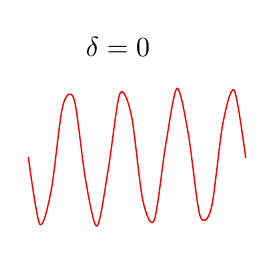
\begin{tikzpicture}
  \begin{scope}[draw=black,line join=round, miter limit=4.00,line width=0.5pt,y=1pt,x=1pt] 
    \XYcross;
  \end{scope}
  
  \begin{scope}[domain=0:3.1415, line join=round, miter limit=4.00,line width=0.5pt, 
                x=25pt,y=25pt, xshift=0, yshift=0]    
    \node at(1.9,1.6) [left, fill=white] {$\delta=0$}; %                         
    \draw[color=red] plot[id=myfce, samples=20, smooth] (\x, {sin(30*\x r)}); % 
  \end{scope}  
\end{tikzpicture}}                              \\
        \end{tabular}
        \caption{a) Modulové charakteristiky paralelního rezonančního obvodu pro napěťový přenos.
                 b) model paralelního rezonančního obvodu a jeho napájení ze zdroje o proměnném 
                 kmitočtu, c) přeměna rezonančního obvodu v oscilátor, d) časová závislost napětí 
                 na svorkách ztrátového LC obvodu po rozkmitání, d) výstupní napětí bezeztrátového 
                 LC obvodu 
                 \cite[s.~135]{Dolecek2009}.}
        \label{AES:fig_MUE6_311}
      \end{figure}
      
      Na obr. \ref{AES:fig_MUE6_311c} je nakreslen paralelní rezonanční obvod, u kterého do obvodu 
      po přepnutí spínače z polohy \(1\) do polohy \(2\) připojujeme předem nabitý kondenzátor. V 
      obvodu vzniknou vlastní tlumené kmity o kmitočtu \(\omega_0\). Obvod lze popsat diferenciální 
      rovnicí
      \begin{equation}\label{AES:eq_osc04}
        \dder{i}{t} + \frac{R}{L}\cdot\der{i}{t} + \omega^2 i = 0
      \end{equation}
      Rovnice má řešení
      \begin{equation}
        i(t) = I_{0}e^{-\delta t}\sin\omega_v t  \qquad u(t) = U_{0}e^{-\delta t}\cos\omega_v t
      \end{equation}
      kde \(I_0\) je \emph{počáteční amplituda proudu}, \(U_0\) je \emph{počáteční amplituda napětí 
      na kapacitoru}, \(\delta = \frac{R}{2L}\) je \textbf{činitel tlumeni obvodu}, \(\omega_0 
      =\frac{1}{\sqrt{LC}}\) je \textbf{rezonanční kmitočet} a \(\omega_v = \sqrt{\omega^2_0 - 
      \delta^2}\) je \textbf{vlastní kmitočet volných kmitů} obvodu. 
      
      Ze vztahu (\ref{AES:eq_osc04}) je zřejmé, Že je-li činitel tlumeni a \textbf{kladný} je 
      kmitání \textbf{tlumené}, je-li a \textbf{záporný} je kmitání \textbf{netlumené}, je-li 
      \(\delta = 0\) mají kmity konstantní amplitudu. Velikost činitele tlumení je závislá na 
      velikosti rezistoru \(R\), který modeluje ztráty v rezonančním obvodu viz obr. 
      \ref{AES:fig_MUE6_311d}, \ref{AES:fig_MUE6_311e}.
      
      V reálném obvodu je vždy \(\delta > 0\) a proto pozorujeme tlumené kmity, jejichž amplituda 
      klesá exponenciálně podle vztahu 
      \begin{equation}\label{AES:eq_osc02}
        u(t) = U_{ss}e^{-\delta t},
      \end{equation}
      kde \(u(t)\) představuje časovou závislost amplitudy kmitů na svorkách paralelního LC obvodu. 
      Dosáhnout nulového tlumení je možné sériovým zapojením rezistoru \(-R_N = R\) - tedy 
      rezistoru se \textbf{záporným odporem}. K tomu by bylo zapotřebí najít takovou součástku, 
      jejíž voltampérová charakteristika vykazuje úsek se zápornou derivací. Hledáme tedy součástky 
      které mají voltampérovou charakteristiku jako je na obr. \ref{AES:fig_AES62a} nebo 
      \ref{AES:fig_AES62b}.
      
      \begin{figure}[ht!]
        \centering  
        \begin{tabular}{cc}
          \subfloat[nelinearita typu \textbf{S}]{\label{AES:fig_AES62a}
            %\documentclass{article}
%\url{http://tex.stackexchange.com/q/82308/86}
%\usepackage{tikz}

\def\xmin{20}
\def\xmax{220}
\def\ymin{-5}
\def\ymax{+220}
\def\zero{0}
\def\phase{25bp}
\def\xlabel{$u$}
\def\ylabel{$i$}

\def\curveS{%
\pgfpathmoveto {\pgfqpoint{25bp}{0bp}} 
\pgfpathcurveto{\pgfqpoint{25bp}{0bp}}
               {\pgfqpoint{104bp}{51bp}}
               {\pgfqpoint{104bp}{69bp}}
\pgfpathcurveto{\pgfqpoint{104bp}{83bp}}
               {\pgfqpoint{72bp}{84bp}}
               {\pgfqpoint{85bp}{101bp}}
\pgfpathcurveto{\pgfqpoint{97bp}{116bp}}
               {\pgfqpoint{176bp}{198bp}}
               {\pgfqpoint{176bp}{198bp}}  
\pgfusepath{stroke}} 

\def\curveN{%
\pgfpathmoveto {\pgfqpoint{25bp}{0bp}}  
\pgfpathcurveto{\pgfqpoint{25bp}{0bp}} 
               {\pgfqpoint{35bp}{65bp}} 
               {\pgfqpoint{53bp}{74bp}}
\pgfpathcurveto{\pgfqpoint{74bp}{83bp}}  
               {\pgfqpoint{89bp}{44bp}}
               {\pgfqpoint{121bp}{59bp}}
\pgfpathcurveto{\pgfqpoint{153bp}{73bp}} 
               {\pgfqpoint{176bp}{198bp}}
               {\pgfqpoint{176bp}{198bp}}  
\pgfusepath{stroke}} 


%\begin{document}

\begin{tikzpicture}[scale=0.3]
  \begin{scope}[draw=black,line join=round, miter limit=4.00,line width=0.5pt,y=1pt,x=1pt] 
    \curveS;
%   \curveN;
    \XYcross;
  \end{scope}  
\end{tikzpicture}

%\end{document}
}                              &
          \subfloat[nelinearita typu \textbf{N}]{\label{AES:fig_AES62b}
            \input{../src/AES/img/AES_62b.tex}}                              
        \end{tabular}
        \caption{Voltampérové charakteristiky s úseky vykazující záporný diferenciální odpor 
        \cite[s.~93]{Koucky1997}}
        \label{MIT:fig_AES_62}
      \end{figure}
      
      Pro sériový model kmitavého obvodu obr. \ref{AES:fig_AES63a} je použitelná nelinearita 
      \texttt{typu S} (např. lavinová dioda), pro paralelní model kmitavého obvodu obr. 
      \ref{AES:fig_AES63b} je použitelná nelinearita \texttt{typu N} (např. tunelová dioda) 
      \cite[s.~93]{Koucky1997}.

      \begin{figure}[ht!]
        \centering  
        \begin{tabular}{cc}
          \subfloat[sériový rezonanční obvod]{\label{AES:fig_AES63a}
            \documentclass{standalone}
    \usepackage{xltxtra}
    \usepackage{tikz}
    \usetikzlibrary{intersections, calc}
    \usepackage[
        american, 
        europeanresistors,
        cuteinductors,  
        smartlabels]{circuitikz}
        \usetikzlibrary{shapes} 
        \ctikzset{bipoles/thickness=1}
        \ctikzset{bipoles/length=0.8cm}
        \ctikzset{bipoles/vsourceam/height/.initial=.7}
        \ctikzset{bipoles/vsourceam/width/.initial=.7}
        \tikzstyle{every node}=[font=\small]
        \tikzstyle{every path}=[line width=0.8pt,line cap=round,line join=round]
\begin{document}
    \begin{circuitikz}
        \draw
        (0,0)
            to[L, l^=$L$] ++(0,2)
            to[short] (2,2)
            to[C, l=$C$] ++(0,-2)
            to [R, l_=$R_N$] ++ (-1,0)
            to [R, l_=$R$] ++ (-1,0) 
            --(0,0);
    \end{circuitikz}
\end{document}    }                              &
          \subfloat[paralelní rezonanční obvod]{\label{AES:fig_AES63b}
            \documentclass{standalone}
    \usepackage{xltxtra}
    \usepackage{tikz}
    \usetikzlibrary{intersections, calc}
    \usepackage[
        american, 
        europeanresistors,
        cuteinductors,  
        smartlabels]{circuitikz}
        \usetikzlibrary{shapes} 
        \ctikzset{bipoles/thickness=1}
        \ctikzset{bipoles/length=0.8cm}
        \ctikzset{bipoles/vsourceam/height/.initial=.7}
        \ctikzset{bipoles/vsourceam/width/.initial=.7}
        \tikzstyle{every node}=[font=\small]
        \tikzstyle{every path}=[line width=0.8pt,line cap=round,line join=round]
\begin{document}
    \begin{circuitikz}
        \draw (0,0)
            to[L, l^=$L$] ++(0,2)
            to[short] ++(3,0) to [R, l=$R_N$] ++ (0,-2) --(0,0);    
        \draw (1,2) to[C, l=$C$,*-*] ++(0,-2);
        \draw (2,2) to [R, l=$R$,*-*] ++ (0,-2);
    \end{circuitikz}
\end{document}}                              
        \end{tabular}
        \caption{ }
        \label{MIT:fig_AES_63}
      \end{figure}
      
      Na velikosti ztrátového odporu \(R\) závisí velikost činitele tlumení \emph{(damping factor)} 
      obvodu podle vztahu:
      \begin{equation}\label{AES:eq_osc01}
        \delta = \frac{R}{2L} \qquad [rad/s]
      \end{equation}
      
      LC oscilátory obsahují klasický rezonanční obvod, jehož rezonanční kmitočet je určen 
      \textbf{Thomsonovým vztahem}:
      \begin{equation}\label{AES:eq_osc03}
        f_0 = \frac{1}{2\pi\cdot\sqrt{LC}} \quad [Hz], \;\text{nebo}\; 
        \omega_0 = \frac{1}{\sqrt{LC}} \quad [rad/s].
      \end{equation}
      
} % tikzset
%---------------------------------------------------------------------------------------------------
\printbibliography[title={Seznam literatury}, heading=subbibliography]
\addcontentsline{toc}{section}{Seznam literatury}
%=============== Kapitola: Operační zesilovače ====================================================
%  % !TeX spellcheck = cs_CZ
{\tikzset{external/prefix={tikz/AES/}}
 \tikzset{external/figure name/.add={ch04_}{}}
%---------------------------------------------------------------------------------------------------
% file opamp.tex
%---------------------------------------------------------------------------------------------------
%================================ Kapitola: Zesilovače==============================================
\chapter{Operační zesilovače}
\minitoc
  \section{Úvod}
    \emph{Operační zesilovače} (\texttt{OZ}, aj: \texttt{opamp}) původně vznikly jako složité 
    elektronické obvody pro náročné použití při zpracování analogových (spojitě se měnících) 
    stejnosměrných a nízkofrekvenčních střídavých signálů v analogových počítačích. Moderní 
    polovodičová technologie umožnila vytvoření \texttt{OZ} v podobě levných integrovaných obvodů s 
    malým počtem vývodů, které mají nepatrnou spotřebu, jsou odolné proti přetížení a umožňují 
    jednoduše realizovat nejrůznější elektronická zařízení.
  
    Svůj název získaly z dob \emph{analogových počítačů}, ve kterých se používaly k realizaci 
    matematických operací. Tyto integrované obvody se svými vlastnostmi blíží \emph{ideálním 
    zesilovačům napětí}. Jejich zesílení bez vnější zpětné vazby se blíží nekonečnu ($10^7$). 
    Vstupní odpor je velmi velký ($10^4 \Omega$) a výstupní odpor je malý ($10 \Omega$). Kmitočtový 
    rozsah sahá od stejnosměrného signálu do desítek megahertzů. Vlastní šum a zkreslení zesilovače 
    jsou rovněž malé. V dnešním pojetí je možné vymezit operační zesilovač jako 
    \textbf{stejnosměrný zesilovač} s velkým zesílením a malým vlastním rušením, schopný stabilní 
    činnosti v uzavřené zpětnovazební smyčce \cite[s.~5]{Dostal}.

    Směr signálového toku operačním zesilovačem (dále je OZ) od vstupu k výstupu je vyznačen 
    trojúhelníkovým tvarem jeho symbolické značky na obr. \ref{AES:OP_znacka}.
    \begin{figure}[ht!]
      \centering
      \includegraphics[width=\linewidth]{Dosta_OP_znacka.pdf}
      \caption[Symbolická značka OP]{Symbolická značka OP s vyznačenými signálovými svorkami (a) 
               a skutečná realizace zemní svorky (b, c)}
      \label{AES:OP_znacka}
    \end{figure}
  
    \textbf{Shrnutí}
    \begin{enumerate}\addtolength{\itemsep}{-0.5\baselineskip}
      \item Operační zesilovač má čtyři signálové svorky, i když se často kreslí jen tři - oba 
            vstupy a výstup. Čtvrtou signálovou svorkou je zem.
      \item Souhlasné napětí $u_{CM}$ je totožné s napětím jeho neinvertujícího vstupu $u^+$.
      \item Ideální operační zesilovač má za všech okolností nulové diferenční vstupní napětí a  
            nulové vstupní proudy.
    \end{enumerate}
  
  \section{Parametry operačního zesilovače}
    Ideální operační zesilovač je nedosažitelná abstrakce. K posouzení kvality sku\-teč\-ného 
    operačního zesilovače slouží řada funkčních parametrů jako soubor dat, která lze zjistit 
    měřením na svorkách.
   
    Operační zesilovač, jako každý aktivní elektronický obvod, je obvod nelineární. Funkční 
    charakteristiky OZ však připouštějí linearizaci bez přílišného odklonu od skutečnosti. 
    Odpovídající kvazilineární parametry jsou podkladem lineárního modelu OZ. Ostatní parametry 
    jsou podstatné nelinearity, které tvoří meze jeho lineární oblasti.
    
    \subsection{Lineární parametry a lineární model}
      Obr. \ref{AES:fig_lin_model_opamp} ukazuje úplný \emph{lineární} model operačního zesilovače. 
      Se zřetelem k pozdější analýze chyb operačního obvodu je vhodné rozdělit znázorněné lineární 
      parametry na \textbf{aditivní} a \textbf{multiplikativní}.
      \begin{itemize}\addtolength{\itemsep}{-0.5\baselineskip}
        \item Aditivní parametry zahrnují náhradní rušivé zdroje náhodných fluktuací: $E_R$, 
              $I_R^-$, $I_R^+$, které způsobují aditivní chyby operačního obvodu nezávislé na jeho 
               signálovém vybuzení.
        \item Multiplikativní parametry představované čtyřmi odpory $R_D, R^-_{CM}, R^+_{CM}$,  
              $R_0$ a dvěma řídicími konstantami $-A, 1/X$ závislých generátorů, vystihují pasivní 
              a přenosové vlastnosti OZ způsobují multiplikativní chyby operačních obvodu úměrné 
              jeho signálovému vybuzení.
      \end{itemize}
      Vnitřní, na svorkách neměřitelný napěťový úbytek $e_D$ na odporu $R_D$ zastává v tomto modelu 
      vazbu mezi vstupem a výstupem.
     
      Při práci s proměnnými signály v časové nebo frekvenční oblasti se  význam použitých symbolů 
      vhodně rozšíří na impedance, operátorové přenosy apod.
      \begin{figure}[ht!]
        \centering
        \includegraphics[width=\linewidth]{Dostal_Opamp_model.pdf}
        \caption[Lineární model operačního zesilovače]{Lineární model operačního zesilovače}
        \label{AES:fig_lin_model_opamp}
      \end{figure}
  
    \subsection{Nelineární parametry}
      Chyby, které provázejí aproximaci skutečného operačního zesilovače lineár\-ním modelem, se 
      zvětšují se vstupním a výstupním vybuzením. To se týká zejména linearizace převodní 
      charakteristiky naprázdno $u_0(u_D)$ výrazem $-A(u_D-E_R-e_{CM})$, výstupní charakteristiky 
      $u_0(i_0)$ výrazem $e_0-R_0i_0$ a vstupní charakteristiky $e_{CM}(u_{CM})$ výrazem 
      $u_{CM}/X$.  Skutečný průběh každé z těchto charakteristik se vyznačuje velmi ostrým kolenem, 
      při jehož překročení ztrácejí lineární parametry smysl.  Signálové vybuzení, které přísluší 
      tomuto kolenu, tak vymezuje dosti přesně oblast lineárního chování \cite[s.~29]{Dostal}.
  
      Třem svorkovým proměnným $u_{CM}, u_O, i_0$ přísluší tři \emph{statické nelinearity} (omezení 
      rozkmitu) a tři dynamické nelinearity (omezení rychlosti)
  
  \section{Ideální operační obvod}
    \subsection{Paralelní operační obvod}
      \fbox{Napěťový invertor} ukazuje, že vstupní signálový proud může být generován také 
      synteticky, kombinací napěťového signálového zdroje a sériového rezistoru. Takovým způsobem 
      vytvořený \emph{napěťový invertor} na obr. * je jedním z nejčastějších operačních obvodů. 
      
      Vstupní napětí $u_s$ je celé vloženo na rezistor $R_1$ (jeho pravý konec je virtuálně 
      uzemněn) a vyvolává ekvivalentní vstupní proud $\frac{u_s}{R_1}$. Tento přitékající proud je 
      kompenzován proudem $-\frac{u_0}{R_2}$ odsávaným přes zpětnovazební rezistor $R_2$ do výstupu 
      operačního zesilovače $$\frac{u_s}{R_1}=-\frac{u_0}{R_2}.$$ Ideální operační rovnice
      \begin{equation}\label{AES:eq_opamp_inv02}
        u_0 = - \frac{R_2}{R_1}u_s.
      \end{equation}
      Vyjadřuje úměrnost signálových napětí $-u_0$ a $u_s$ velikostem přilehlých rezistorů $R_2$ a 
      $R_1$. Pro snadnější zapamatování se nabízí představa dvouramenné páky s délkami ramen $R_1$ 
      a $R_2$, otočné v bodě odpovídajícímu virtuální zemi, která přenáší výchylku $u_s$ levého 
      konce na výchylku $u_0$ pravého konce v opačné polaritě.

      \begin{figure}[ht!]
        \centering
        \begin{tabular}{c}
          \subfloat[$u_0 = -\dfrac{R_2}{R_1}u_s, \qquad R_{||} = R_1, \qquad R_{\mathsf{O}|} = 
          0$]{\label{{ES:fig_004a}}
            \includegraphics[width=0.5\linewidth]{opamp_inv01a.pdf}}             \\
          \subfloat[ $u_0 = -\dfrac{R_2}{R_2+R_s}u_s$ ]{\label{AES:fig_004b}
            \includegraphics[width=0.51\linewidth]{opamp_inv01b.pdf}}             
        \end{tabular}
        \caption{Napěťový invertor. Jeho mechanickou analogií je dvouramenná páka (a). Přítomnost 
                 vnitřního odporu signálového zdroje $R_s$ v operační rovnici je důsledkem 
                 konečného vstupního odporu $R_{||} = R_1$ (b). }
        \label{AES:fig_opamp_inv01} 
      \end{figure}
      Zesílení napěťového invertoru 
      \begin{equation}\label{AES:eq_opamp_inv01}
        G_i = -\frac{R_2}{R_1},
      \end{equation} 
      je záporné a nastavitelné v širokých mezích od $0$ do $\infty$ výběrem rezistorů $R_1$ a 
      $R_2$. Zvláštním případem je jednotkový invertor se stejnými rezistory $R_1 = R_2$, který 
      prostě invertuje polaritu vstupního napětí: $$u_0 = - u_s, \qquad G_i = -1.$$
      
      Výstupní odpor napěťového invertoru je ideálně nulový. Jeho vstupní odpor však ztrácí onen 
      vyhranění charakter typický pro kanonické operační obvody a nabývá indiferentní velikosti 
      \begin{equation}\label{AES:eq_opamp_inv03}
        R_{||} = R_1,
      \end{equation} 
      rovné velikosti virtuálně uzemněného rezistoru $R_1$.
      
      Napěťový invertor zatěžuje signálový zdroj (obr. *). To se projevuje poklesem svorkového 
      napětí signálového zdroje o úbytek na vnitřním odporu $R_s$, nebo jinak řečeno, přítomností 
      nedefinovaného a nestálého vnitřního odporu $R_s$ v operační rovnici invertoru:  
      \begin{equation}\label{AES:eq_opamp_inv04}
       u_0 = -\frac{R_2}{R_1 + R_s}u_s.
      \end{equation}      
      Taková vlastnost se obvykle považuje za nedostatek. 
            
    \subsection{Sériový operační obvod}
    
    \subsection{Složený operační obvod}
      Operační obvody, které není možné zahrnout do předcházejích dvou velkých tříd, se vyznačují:
        \begin{itemize}\addtolength{\itemsep}{-0.5\baselineskip}
          \item signálovým buzením obou vstupů operačního zesilovače,
          \item násobnou zpětnou vazbou,
          \item kombinací záporné a kladné zpětné vazby,
          \item použitím několika operačních zesilovačů,
          \item nestandardním zapojením operačního zesilovače.
        \end{itemize}
      \subsubsection{Signálové buzení obou vstupů}
        \fbox{Rozdílový zesilovač} na obr. \ref{AES:fig_diff_opamp01} je lineární operační obvod se dvěma vstupy. Jeho výstupní napětí se najde superpozicí \cite[s.~126]{Dostal}. 
        
        Nechť působí napětí $u_1$ a napětí $u_2$ je nulové. Neinvertující vstup operačního 
        zesilovače je uzemněn přes paralelní kombinaci rezistorů $R_3$ a $R_4$. Operační obvod 
        představuje napěťový invertor a první složka výstupního napětí má velikost 
        $$-\frac{R_2}{R_1}u_1.$$
        
        Nechť působí napětí $u_2$ a napětí $u_1$ je nulové. Operační obvod představuje neinvertujcí 
        zesilovač s předřazeným děličem $R_3$ a $R_4$ a druhá složka výstupního napětí má velikost 
        $$u_2\frac{R_4}{R_3+R_4}\left(\frac{R_2}{R_1}+1\right)= 
        u_2\frac{R_2/R_1+1}{R_4/R_3+1}\cdot\frac{R_4}{R_3}.$$
        
        %----------------------------------
        % image: rozdílový zesilovač
        % !TeX spellcheck = cs_CZ
% Diferenciální zesilovač
% pozn: symbol země (ground) je předefinován v knihovně wiking.sty

% Define box and box title style
% http://www.texample.net/tikz/examples/boxes-with-text-and-math/
\tikzstyle{mybox} = [draw=red, fill=blue!20, very thick,
    rectangle, rounded corners, inner sep=5pt, inner ysep=10pt, inner xsep=10pt ]
\tikzstyle{fancytitle} =[fill=red, text=white]

\begin{figure*}[ht!]
  \centering
  \begin{circuitikz}[scale=1, every node/.style={scale=1}]
    \ctikzset{resistor=european}
%    \ctikzset{tripoles/op amp/scale=0.5}
    \draw (0,0) node[op amp, scale=0.5] (opamp) {};
    \node [left=0.1cm of opamp.-]       (p1) {};
    \node [left=0.1cm of opamp.+]       (p2) {};
    \node [above=0.5cm of p1]           (A)  {};
    \node [left=1.5cm of A]             (p3) {};
    \node [right=1.5cm of A, coordinate](C)  {};
    \node [right=0.5cm of C]            (p6) {};
    \node [below=0.5cm of p2]           (B)  {};
    \node [left=1.5cm of B]             (p4) {};
    \node [right=1.5cm of B]        (ground) {};
    \node [right=0.1cm of opamp.out, coordinate] (vo) {};
    %%% Draw connections
    \draw (p3) node[left] {$u_1$} to[R=$R_1$,o-] (A)  to[R=$R_2$,*-] (C); 
    \draw (opamp.-)   to[short] (p1) to[short] (A);
    \draw (opamp.out) to[short] (vo);
    \draw (vo) to[short,-*] (vo |- C); 
    \draw (p4) node[left] {$u_2$} to[R=$R_3$,o-] (B)  to[R=$R_4$,*-] (ground) node [sground] {};  
    \draw (opamp.+) to[short] (p2) to[short] (B); 
    \draw (C) to[short,-o] (p6) node[right] {$u_{0}$};
    \node[above] at (A) {A}; % text 
    \node[below] at (B) {B}; % text 
    %%% minipage
    \node [mybox, right=5cm of p2] (box){%
       \begin{minipage}[l]{3cm}
          \begin{align*}
              \frac{R_4}{R_3} &= \frac{R_2}{R_1} \\
              u_0             &= \frac{R_2}{R_1}(u_2 - u_1) \\
              R_{|1|}         &= R_1 \\
              R_{|2|}         &= R_3 + R_4 \\
              R_{\mathsf{O}|} &= 0
          \end{align*}
       \end{minipage}
    };
    \node[fancytitle, right=10pt, rounded corners] at (box.north west) {rovnice:};
   %\node[fancytitle, rounded corners] at (box.east) {$\clubsuit$};
    %%% text R_{|1|} and R_{|2|}
    \draw[->] (-4.0,0.2) -- +(0,0.5) node[left] {$R_{|1|}$} -- +(0.5,0.5);
    \draw[->] (-4.0,-0.2) -- +(0,-0.5) node[left] {$R_{|2|}$} -- +(0.5,-0.5);
  \end{circuitikz} 
  \caption{Rozdílový zesilovač. Podmínky potlačení souhlasné složky vstupních napětí $u_1$ a 
           $u_2$ je poměrové vyvážení zpětnovazebních rezistorů, $R_4/R_3 = R_2/R_1$. S ohledem na 
           ofset se obvykle volí uplná symetrie, tj. $R_4 = R_2$ a $R_3 = R_1$.}
  \label{AES:fig_diff_opamp01}         
\end{figure*} 
        %---------------------------------- 
               
        Současné působení obou vstupních napětí ve vyváženém operačním obvodě $$\frac{R_4}{R_3}=\frac{R_2}{R_1},$$ přísluší výstupní napětí 
        \begin{equation}\label{AES:eq_diff_opamp}
          u_2 = \frac{R_2}{R_1}(u_2-u_1),   
        \end{equation}
        úměrné rozdílu vstupních napětí bez ohledu na jejich absolutní velikost. Odtud název 
        operačního obvodu. Důvod zařazení napěťového děliče ($R_3$,$R_4$) je zřejmý - dělič 
        sjednocuje zesílení invertujícího a neinvertujícího vstupu, která se liší absolutně o 
        jednotku. 
        
        Dvěma vstupům přísluší dva vstupní odpory. První vstupní odpor $$R_{|1|} = R_1$$ je roven 
        velikosti rezistoru $R_1$, protože vnitřní odpor bodu $A$\footnote{obdoba virtuální země} 
        je nulový. Druhý vstupní odpor $$R_{|2|} = R_3 + R_4$$ je roven součtu rezistorů $R_3$ a 
        $R_4$, protože vnitřní odpor zbytku operačního obvodu v bodě $B$ je nekonečný. Tyto dva 
        vstupní odpory jsou různé, i když jsou obě větve ($R_1$, $R_2$) a ($R_3$, $R_4$) stejné. 
        
        Vstupní odpory $R_{|1|}$ a $R_{|2|}$ přísluší dvěma samostatným uzemněným zdrojům 
        signálových napětí $u_1$ a $u_2$ podle \ref{AES:fig_diff_opamp01}. Volnému (izolovanému) 
        signálovému napěťovému zdroji připojenému diferenčně mezi vstupy rozdílového zesilovače, by 
        příslušel diferenční vstupní odpor $$R_{|D|} = R_1 + R_3,$$ rovný součtové velikosti 
        rezistorů $R_{|1|}$ a $R_{|3|}$, protože body $A$ a $B$ jsou virtuálně zkratovány.

} % tikzset
%---------------------------------------------------------------------------------------------------
\printbibliography[title={Seznam literatury}, heading=subbibliography]
\addcontentsline{toc}{section}{Seznam literatury}
  
%=============== Kapitola: Systémy pro digitální zpracování analogového signálů ===================
%  % !TeX spellcheck = cs_CZ
%---------------------------------------------------------------------------------------------------
% file DA_AD_converter.tex
%---------------------------------------------------------------------------------------------------
%======================= Kapitola: Konverze mezi digitálním a analogový signálem====================
\setchaptertoc
\chapter{Konverze mezi digitálním a analogový sig\-ná\-lem}


\section{Konverze mezi digitálním a analogový signálem}
  Při zpracování analogového signálu je jednou z důležitých funkcí převod tohoto signálu z analogové
  podoby do číslicové a naopak. Proto jsou analogově-číslicové převodníky resp. číslicově-analogové
  převodníky (ADC - Analog-to-Digital Converter), (DAC - Digital-to-Analog Converter) velmi
  důležitými prvky jakéhokoli systému zpracovávajícího signál \cite[s.~11]{Haze}. Na obrázku
  \ref{AES:fig_ADC_DAC_IO} je definováno rozhraní obou typů převodníku.
  \begin{figure}[ht!]
     \centering
     \includegraphics[width=\linewidth]{ADC_DAC_block.pdf}
     \caption[Definice I/O bloku DAC a ADC ]{Definice rozhraní bloku analogově-číslicového (ADC) a 
              číslicově-analogového (DAC) převodníku}
     \label{AES:fig_ADC_DAC_IO}
  \end{figure}

  \textbf{Analogově-číslicové převodníky} (Analog-to-Digital Converters) slouží k pře\-ve\-de\-ní 
  analogového signálu na signál číslicový. Pro A/D převodník má analogová stupnice vstupního 
  signálu délku \texttt{FS} (\emph{Full scale}), udávanou např. ve voltech. Stupnice číslicového 
  signálu pak vyznačuje diskrétní hodnoty výstupu, které převodník generuje při převodu analogového 
  signálu \cite[s.~202]{Neumann}.

  \textbf{Číslicově-analogové převodníky} (Digital-to-Analog Converters) slouží k o\-pač\-né\-mu 
  procesu, tedy k pře\-ve\-de\-ní číslicového signálu na signál analogový, což by šlo realizovat 
  pomocí lineárního digitálního potenciometru a připojeného zdroje referenčního napětí na jeho 
  vstupu \cite[s.~208]{Neumann}. Pro N-bitové binární slovo by musel mít $n-1$ rezistorů a $n$ 
  resp. $2n - 1$ spínačů. To je monoliticky téměř nerealizovatelné již pro osmi- a vícebitové 
  slovo. Řešení převodníků proto musí být mnohem úspornější, i když úspory budou vykoupeny jinými 
  nevýhodami, případně omezeními pro jejich použití.

    \subsection{Základní struktura převodníků}
      Obě skupiny převodníků mohou typicky obsahovat komparátory, číslicové obvody, spínače, 
      integrátory, vzorkovací obvody a/nebo pasivní součástky. Nezbytnou a důležitou součástí je i 
      přesný zdroj referenčního napětí. V mnoha případech pak také platí, že DAC je jednou z částí 
      ADC.
      
      Analogově číslicový převod můžeme pomyslně rozložit do tří etap \cite{Sebesta}.
      \begin{enumerate}[noitemsep]
        \item Převod signálu se spojitým časem na signál s diskrétním časem. Tomuto převodu říkáme  
              vzorkování.
        \item Kvantování vzorku s cílem vyjádřit vzorky konečnou množinou čísel. Tento krok je 
              provázen vznikem tzv. kvantovacího šumu. Uvedený jev souvisí s nelineárním zkreslením 
              známým z teorie obvodů.
        \item Kódování spočívající zpravidla v binárním vyjádření čísel představujících velikosti  
              vzorku.
      \end{enumerate}
      
    \subsection{Statické a dynamické parametry převodníků}
      Statické parametry převodníků jsou určovány pomocí \emph{převodní charakteristiky}, zatím co
      dynamické vlastnosti se vyhodnocují z kmitočtového spektra převodníku \cite[s.~11]{Haze}.
      \begin{itemize}[noitemsep]
        \item rozsah,
        \item integrální a diferenciální nelinearita (\emph{integral - INL, differential - DNL nonlinearity}),
        \item rozlišení převodníku (\emph{resolution}),
        \item přesnost (\emph{accuracy}),
        \item chyba monotónnosti,
        \item chyba nastavení nuly (\emph{offset error}),
        \item hystereze a další.
       \end{itemize}
       K hlavním dynamickým parametrům patří
       \begin{itemize}[noitemsep]
         \item odstup signál - šum (\emph{signal to noise ratio - SNR}) kap. \ref{AES:cap_SNR},
         \item efektivní počet bitů (\emph{effective number of bits - ENOB}),
         \item harmonické zkreslení (\emph{total harmonic distortion - THD}),
         \item odstup signál-šum a zkreslení (\emph{signal to noise and distortion - SINAD}),
         \item dynamický rozsah bez parazitních složek \newline(\emph{spurious free dynamic range 
               - SFDR}),
         \item šum - vrcholový, efektivní (\emph{noise - peak, rms}),
         \item doba přepnutí a ustálení.
       \end{itemize}

    \subsection{Vzorkování}
    \subsection{Kvantování}
       Pro přechod od časově spojitého signálu se spojitou množinou hodnot k číslicovému signálu, 
       je nutné provést (výškové) \texttt{kvantování}, tj. kvantování hodnot signálu, které je 
       patrné z obrázku \ref{AES:fig_Quntized_sig_wave}. Je zřejmé, že mapování spojitého intervalu 
       vstupních hodnot na diskrétní hodnoty digitálního výstupu způsobí, že každá hodnota 
       digitálního výstupu platí pro vstupní signál měnící se v určitém  podintervalu. Délka 
       podintervalu, pro který platí jedna hodnota digitálního výstupu se nazývá 
       \textbf{kvantizační krok převodníku} - \emph{Q}, jenž je roven bitu s nejnižší váhou - 
       \texttt{LSB}.

       \begin{figure}[ht!]
         \centering
         \includegraphics[width=1\linewidth]{ADC_DAC_3bit.pdf}
         \caption[Přenosová funkce AD a DA převodníku]{Ideální přenosová funkce 3bitového    
                  unipolárního AD a DA převodníku. V případě DA převodníku je přenosová funkce 
                  tvořena osmi body, nikoliv čárou.}
         \label{AES:fig_3b_DAC_ADC}
       \end{figure}
 
       Převodní charakteristika DA i AD převodníku je znázorněna na obr. \ref{AES:fig_3b_DAC_ADC}. 
       Analogový signál je spojitý a číslicový signál vyjadřuje jen jeho vybrané diskrétní hodnoty. 
       Proto je převodní charakteristika nespojitá. Naproti tomu digitální vstup vytvoří na výstupu 
       pouze omezený počet hodnot výstupního signálu.

       \begin{figure}[ht!]
         \centering
         \includegraphics[width=1\linewidth]{Uni_Bi_Converter.pdf}
         \caption[Unipolární a bipolární převodníky]{Unipolární a bipolární převodníky \cite{Kester2004}}
         \label{AES:fig_uni_bi_converter}
       \end{figure}

       Počet úrovní AD převodníku, do kterého je rozdělen rozsah vstupního analogového signálu 
       definuje \textbf{rozlišovací schopnost ADC} a lze ji vyjádřit různými způsoby, jak ukazuje 
       tabulka \ref{AES:tab_10b_ADC_resolution} pro 2 až 24bitového převodníku.

         \begin{table*}[ht!]
           \centering
            \setlength{\tabcolsep}{5pt}
            \begin{tabular}{|c|c|c|c|c|c|}
              \hline
                \textbf{Rozlišení} & \multirow{2}{*}{$\mathbf{2^N}$} &  \textbf{Napětí} & 
                \multirow{2}{*}{\textbf{ppm FS}}& \multirow{2}{*}{\textbf{\% FS}}&   
                \multirow{2}{*}{\textbf{dB FS}}                                                 \\
                         N     &           &  \textbf{10V FS} &        &             &          \\
              \hline
                       2-bit   &         4 &            2.5 V & 250000 &          25 &  -12     \\
              \hline
                       4-bit   &        16 &           625 mV &  62500 &        6,25 &  -24     \\
              \hline
                       6-bit   &        64 &           156 mV &  15625 &        1,56 &  -36     \\
              \hline
                       8-bit   &       256 &          39,1 mV &   3906 &        0,39 &  -48     \\
              \hline
                      10-bit   &      1024 &          9,77 mV &    977 &       0,098 &  -60     \\
              \hline
                      12-bit   &      4096 &          2.44 mV &    244 &       0,024 &  -72     \\
              \hline
                      14-bit   &     16384 &       610 $\mu$V &     61 &       0,061 &  -84     \\
              \hline
                      16-bit   &     65536 &       153 $\mu$V &     15 &      0,0015 &  -96     \\
              \hline
                      18-bit   &    262144 &         38 $\mu$ &      4 &      0,0004 & -108     \\
              \hline
                      20-bit   &   1048576 &       9.54 $\mu$ &      1 &      0,0001 & -120     \\
              \hline
                      22-bit   &   4194304 &       2.38 $\mu$ &   0,24 &    0,000024 & -132     \\
              \hline
                      24-bit   &  16777216 &           596 nV &   0,06 &    0,000006 & -144     \\
              \hline
           \end{tabular}
           \caption[Kvantizace: Velikost LSB]{Porovnání rozlišovací schopnosti AD převodníku s  
                    různou délkou výstupního slova. Z tabulky vyplývá, že kvantizační krok 
                    24bitového ADC odpovídá velikosti úbytku na rezistoru $2,2 k\Omega$ při teplotě 
                    25°C, který vzniká vlivem tepelného šumu (viz Johnsonův šum) jenž je při šířce 
                    pásma 10 kHz roven 600 nV. }
           \label{AES:tab_10b_ADC_resolution}
         \end{table*}

       \begin{figure}[ht!]
         \centering
         \includegraphics[width=1\linewidth]{Quantized_signal_wave.pdf}
         \caption[Kvantizační chyba]{Kvantizační chyba je rovna rozdílu původního x(t) a kvantovaného signálu v úrovni y(t) \cite{Bennett}}
         \label{AES:fig_Quntized_sig_wave}
       \end{figure}

       %The quantization error for any ac signal which spans more than a few LSBs can be 
       %approximated by an uncorrelated sawtooth waveform having a peak-to-peak amplitude of q, the 
       %weight of an LSB. Although this analysis is not precise, it is accurate enough for 
       %most applications. W. R. Bennett of Bell Laboratories analyzed the actual spectrum of 
       %quantization noise in his classic 1948

       Kvantizační chyba, jejíž průběh je na obr. \ref{AES:fig_Quntized_sig_wave}, v dynamickém 
       režimu, tj. při časových změnách vstupní analogové veličiny, způsobuje \textbf{kvantizační 
       šum}. Ten lze pozorovat např. tehdy, kdy čísla získaná z převodníku A/D jsou vedena do 
       převodníku D/A a jím je analogový signál rekonstruován. Rekonstruovaný signál se jeví jako 
       signál původní, avšak se superponovaným rušivým signálem. Vzájemným odečtení 
       rekonstruovaného a původního signálu, dostaneme samostatný rušivý signál, který lze podrobit 
       analýze. \emph{Pokud je vzorkovací signál nekorelovaný se vzorkovaným signálem, je možno 
       kvantizační šum považovat za náhodný}. Vztah mezi původním signálem a signálem degradovaným 
       kvantizačním šumem vyjadřuje parametr - \texttt{SNR}
       \begin{itemize}
         \item SNR  - Signal to Noise Ratio: poměr signálu k šumu
             \begin{equation}\label{AES:eq_SNR}
                SNR = \frac{E\{x^2(t)\}}{E\{[y(t)-x(t)]^2\}}
             \end{equation}
                \begin{itemize}
                   \item $E\{.\} \cdots$ operátor průměrování
                   \item $x(t)   \cdots$ vstupní analogový signál
                   \item $y(t)   \cdots$ rekonstruovaný kvantovaný signál
                 \end{itemize}
       \end{itemize}
       Kvantizační chybu lze aproximovat nekorelovaným pilovým průběhem s amplitudou špička-špička 
       rovnou kvantizačnímu kroku $Q$. Ačkoliv takto provedená analýza (viz kapitola 
       \ref{AES:kap_kv_sum}) není přesná, v běžných aplikacích zcela postačuje.

       Na obr. \ref{AES:fig_AD_kvantizacni_chyba} je kvantování realizováno tak, že je zajištěna 
       minimální chyba kvantování, tj. převodník provádí operaci zaokrouhlování na nejbližší 
       hodnotu. To znamená, že např. číslo jedna bude generováno vstupem v intervalu $1\pm0,5V$, 
       je-li \texttt{FS} rovno 8V a máme-li k dispozici osm kvantizačních úrovní.

       Převodník, který má v celém intervalu předváděných vstupních hodnot konstantní kvantizační 
       krok, se též označuje jako lineární kvantizér. Převodník s přirozeným binárním kódem o 
       \emph{N} bitech je schopen na analogové straně reprezentovat \emph{n-1} ne\-nu\-lo\-vých 
       úrovní analogové veličiny, přičemž platí
       \begin{equation}\label{AES:eq_AD_kod}
          n = 2^N
       \end{equation}
       A jde-li o lineární N-bitový kvantizér, můžeme vyjádřit kvantizační krok vztahem
       \begin{equation}\label{AES:eq_kvant_krok}
          Q = \frac{FS}{n} = \frac{FS}{2^N}
       \end{equation}
       Nejvyšší úroveň vstupní veličiny \emph{A} pak bude
       \begin{equation}\label{AES:eq_A_max}
          A_{max} = \frac{n-1}{n}+\frac{Q}{2}
       \end{equation}

       V sekvenci bitů binárního čísla generovaného převodníkem se zpravidla první bit, který
       představuje nejvyšší binární řád, označuje \texttt{MSB} (\emph{Most Significant Bit}), tedy
       nejvýznamnější bit. Poslední bit, tj. bit v poloze nejnižšího řádu, má označení \texttt{LSB}
       (\emph{Least Significant Bit}), tedy nejméně významný bit. Je zřejmé, že \texttt{LSB}
       jednoznačně určuje základní krok na ose číslicového signálu. Dojde-li ke změně pouze v
       hodnotě \texttt{LSB}, změní se analogová hodnota právě o kvantizační krok. \texttt{LSB} tedy
       na analogové straně určuje rozlišovací schopnost převodníku. Např. osmibitový převodník má
       rozlišovací schopnost \texttt{FS/256}, tj. přibližně \texttt{0,4\%}. Je-li \texttt{FS = 2V},
       musí rozlišit \texttt{8 mV}\cite[s.~203]{Neumann}.

       Vzhledem k diskretizaci hodnot původního analogového signálu při převodu A/D dochází ke
       \emph{kvantizačním chybám}. Je-li např. vstupní veličinou okamžité napětí $u_a$ a této
       hodnotě odpovídá na výstupu číslo $D$, pak kvantizační chybu $\varepsilon_q$ lze vyjádřit
       takto:
       \begin{equation}\label{AES:eq_kvant_chyba}
          \varepsilon_q = u_a - FS\frac{D}{2^N}
       \end{equation}

      \subsection{Kvantizační šum ideálního N-bitového ADC}\label{AES:kap_kv_sum}

      %The only errors (dc or ac) associated with an ideal N-bit data converter are those related  
      %to the sampling and quantization processes. The maximum error an ideal converter makes when 
      %digitizing a signal is $\pm 1/2 LSB$. The transfer function of an ideal N-bit ADC is shown 
      %in Figure 2.37. The quantization error for any ac signal which spans more than a few LSBs 
      %can be approximated by an uncorrelated sawtooth waveform having a peak-to-peak amplitude of 
      %q, the weight of an LSB.

      %The quantization error for any ac signal which spans more than a few LSBs can be 
      %approximated by an uncorrelated sawtooth waveform having a peak-to-peak amplitude of q, the 
      %weight of an LSB. Although this analysis is not precise, it is accurate enough for most 
      %applications. W. R. Bennett of Bell Laboratories analyzed the actual spectrum of 
      %quantization noise in his classic 1948

      V předchozí kapitole byla nastíněna možnost aproximace kvantizační chyby jaké\-ho\-koliv AC 
      signálu v časové oblasti (viz \ref{AES:fig_Quntized_sig_wave}) nekorelovaným pilovým 
      průběhem, za cenu určité nepřesnosti vyvážené jednodušším matematickým aparátem.

      Vyjděme tedy z převodní charakteristiky ideálního N-bitového převodníku zatížené kvantizační 
      chybou, tak jak je znázorněna na obr. \ref{AES:fig_AD_kvantizacni_chyba}. Z té je patrné, že 
      chyba může v absolutní hodnotě dosáhnout maximálně $e(t) = \frac{Q}{2}$, resp. 
      $\pm\frac{1}{2}LSB$ a v rámci kvantizačním kroku ji lze popsat přímkou se strmostí 
      \texttt{s}: $$e(t) = st, -\frac{Q}{2s}<t<+\frac{Q}{2s}.$$ Statisticky je pravděpodobnost 
      jejího rozložení 1/Q a je rovnoměrná od $-\frac{Q}{2}$ do $+\frac{Q}{2}$.

      \begin{figure}[ht!]
        \centering
        \includegraphics[width=0.8\linewidth]{AD_kvantizacni_chyba.pdf}
        \caption[Převodní charakteristika ideálních převodníků]{Převodní charakteristika 
                 ideálních převodníků a závislost chyby kvantizace na vstupní analogové hodnotě}
        \label{AES:fig_AD_kvantizacni_chyba}
      \end{figure}

      Z výše uvedeného plyne, že okamžitá hodnota kvantizační chyby $\varepsilon_q(t) = y(t) - x(t)$
      může dosáhnout rozkmitu maximálně $\pm \frac{Q}{2}$ a jelikož předpokládáme rovnoměrné
      rozložení hodnot, je hustota pravděpodobnosti amplitud rovna $\frac{1}{Q}$.

      \emph{Kvantizační šum $\sigma^2$ je definován jako výkon (rozptyl) střídavé složky kvantizační
      chyby $\varepsilon_q$ a jeho efektivní hodnotu $\sigma$ můžeme odvodit pomocí věty o druhém
      centrálním momentu nebo výpočtem efektivní hodnoty v časové oblasti.}

        \begin{figure}[ht!]
          \centering
          \subcaptionbox{Hustota pravděpodobnosti kvantizačního šumu \label{AES:fig_kvant_sum1}}
            {\luafigure[0.45]{AD_kvantizacni_sum1.pdf}}
          \subcaptionbox{Kvantizační šum jako funkce času \label{AES:fig_kvant_sum2}}
            {\luafigure[0.45]{AD_kvantizacni_sum2.pdf}}
          \caption{K odvození efektivní hodnoty kvantizačního šumu}
          \label{AES:fig_kvant_sum}
        \end{figure}

        \begin{enumerate}[noitemsep]
          \item V pravděpodobnostním počtu je K-tý moment definován jako: 
                \begin{align*}
                  M_k  &= \int_{-\infty}^{\infty} x^k p(x)dx                           \\
                  \shortintertext{tedy}                      
                  e(t) &= \int_{-\frac{Q}{2}}^{+\frac{Q}{2}}(x - x_0)^2p(x)dx = 
                                 \frac{1}{Q}\int_{-\frac{Q}{2}}^{+\frac{Q}{2}}x^2dx    \\
                       &= \frac{Q^2}{12}
                \end{align*}
          \item V časové oblasti má kvantizační šum pilový průběh viz obr.    
                \ref{AES:fig_kvant_sum2}. Z  definičního integrálu efektivní hodnoty dostaneme $$ 
                \overline{e^2(t)} =               
                \frac{s}{Q}\int_{-\frac{Q}{2}}^{+\frac{Q}{2}}(st)^2dt = \frac{Q^2}{12}.$$ Též 
                můžeme využít znalosti efektivní hodnoty pro průběh tohoto typu: 
                $\frac{U_m}{\sqrt{3}}$ a dosazením za $U_m =\frac{Q}{2}$ získáme opět stejný 
                výsledek jako při výpočtu integrálu
        \end{enumerate}

        Tedy efektivní hodnota kvantizačního šumu ideálního N-bitového převodníku je:
        \begin{equation}\label{AES:eq_ef_kv_sumu}
            e(t) = \frac{Q}{\sqrt{12}}
        \end{equation}
        Předpokládejme na vstupu převodníku ustálený harmonický signál o amplitudě $X$. Dále 
        předpokládejme, že signál s amplitudou $X_m$ by pokryl celý rozsah převodníku $FS$. Pak se 
        dá ze vztahu \ref{AES:eq_SNR} vyjádřit odstup signálu od šumu \texttt{SNR} ideálního 
        \emph{N-bitového} převodníku jako podíl jejich výkonů resp. kvadrátu efektivních hodnot 
        signálu a šumu v decibelech vztahem
        \begin{align*}
          SNR      &= \frac{P_{signal}}{P_{noise}} =     
                      \left(\frac{A_{signal}}{A_{noise}}\right)^2         \\
          SNR_{dB} &= 10\log\frac{P_{signal}}{P_{noise}} =       
                      10\log\left(\frac{A_{signal}}{A_{noise}}\right)^2   \\
                   &= 20\log\frac{A_{signal}}{A_{noise}}                  
        \end{align*}
        \begin{equation}\label{AES:eq_SNR_N}
            SNR  = 1,76 + 6,02N + 20log\left(\frac{X}{X_m}\right)
        \end{equation}

        Lze tedy říci, že každý bit navíc v digitálním výstupu A/D převodníku přinese zlepšení 
        odstupu signálu od šumu o \texttt{6 dB}. Naproti tomu je třeba vědět, že uvedený výraz 
        počítá s harmonickým signálem různého rozkmitu. Při zmenšování amplitudy bude relativní 
        podíl šumu v signálu vyšší. Poměry se také mohou velmi změnit, když signál nebude mít 
        harmonický charakter.

      \subsubsection{Odstup signálu od šumu}\label{AES:cap_SNR}
        Z předchozí kapitoly víme, že SNR je definován jako poměr výkonu signálu k výkonu šumu
        ($v\acute{y}kon = ef. hodnota^2$). Pro samotný kvantizační šum platí:
        \begin{align}
          SNR_{dB} &= 10\log\left(\frac{\dfrac{2^N}{2\cdot\sqrt{2}}\cdot     
                                        Q}{\dfrac{Q}{\sqrt{12}}}\right)^2          \nonumber \\
                   &= N20\log2 + 20\log\frac{\sqrt{12}}{2\cdot\sqrt{12}}           \nonumber \\ 
          SNR_{dB} &= 6,02\cdot N + 1,76dB
        \end{align}

        \begin{figure}[ht!]
            \centering
            \includegraphics[width=0.6\linewidth]{AD_SNR.pdf}
            \caption{}
            \label{AES:fig_SNR}
        \end{figure}

        Tato hodnota platí pouze pro ideální převodník pouze s kvantizační chybou, a sinusový 
        signál s rozkmitem přes celý rozsah převodníku.  Skutečný převodník má ovšem vlivem dalších 
        chyb \texttt{SNR} menší než \texttt{SNR} určený pouze pro kvantizační šum. Tato hodnota se 
        nazývá \texttt{SINAD} nebo \texttt{SNDR} - \emph{Signal-to-Noise and Distortion ratio}.

        Známe-li \texttt{SNR} skutečného převodníku, můžeme určit počet efektivních bitu $N_{ef}$ 
        tzn. \emph{efektivní rozlišitelnost převodníku}. Ten je vždy menší než $N$.
        \begin{equation}\label{AES_eq_N_ef}
            N_{ef} = \frac{SNR - 1,76}{6,02}
        \end{equation}
        
  \section{Principy A/D převodníků}
      Převod analogového signálu na číslo lze uskutečnit několika různými postupy:\cite{Neumann}
      \begin{enumerate}[noitemsep]
        \item Vstupní signál se porovnává s kvantovanou referenční veličinou a komparátory okamžitě 
              vyhodnotí, který z nich je větší. Přímým výstupním údajem je binární číslicové slovo.
        \item Vstupní signál i referenční veličina se v určité časové sekvenci zavádějí do   
              integrátoru a komparátor na jeho výstupu určuje sekvenci impulsů, vypovídající o 
              hodnotě vstupní analogové veličiny. Informací o vstupní veličině dále přenáší počet 
              impulsu, jejich kmitočet nebo kódovaná sekvence impulsů. Tato informace může být 
              převedena číslicovým blokem (obvykle blokem DSP) na binární číslicové slovo.
      \end{enumerate}

      Bývá také používáno třídění na \emph{převodníky s přímým a nepřímým vyhodnocení analogové 
      veličiny}.
      \begin{itemize}
        \item \texttt{Převodníky s přímým vyhodnocením} porovnávají hodnoty analogové veličiny s  
              vybranými kvantizačními úrovněmi současně nebo postupně, a to tak, že každá úroveň má 
              vlastní komparátor. K těmto převodníkům patří \emph{převodníky paralelní a kaskádní}.
        \item \texttt{K nepřímému převodu} můžeme využít postupného provoláváním vstupní
              ve\-li\-či\-ny s vhodnými vzorky referenčního napětí, dodávanými na vstup jediného
              komparátoru v pořadí a velikosti řízené logickými obvody. U těchto převodníků je
              vstupní analogová veličina porovnávaná s výstupní veličinou převodníku \texttt{D/A},
              přičemž je číslicový vstup tohoto převodníku měněn tak, aby se obě veličiny k sobě
              přibližovaly. Pokud se k sobě dostatečně přiblíží, je převod ukončen. I zde jsou v
              podstatě jen dvě jednoduché možnosti přibližování výstup převodníku \texttt{D/A} k
              určité úrovni vstupní veličiny: buď se přibližování děje se stálým krokem, kdy jde o
              krokování po jednotlivých kvantovacích úrovních (\emph{převodníky sledovací}), nebo
              postupnou aproximací (\emph{převodníky aproximační}), kdy první krok rozhoduje o
              hodnotě \texttt{MSB}, další kroky porovnávají binárně zmenšované hodnoty odpovídající
              jednotlivým binárním řádům s tím, že poslední krok určí hodnotu \texttt{LSB}.
        \item Jinou možností nepřímého převodu A/D je převést hodnotu vstupní veličiny na takový  
              parametr pomocného signálu, který se pak dá snadno převést na číslicový údaj. Tímto 
              parametrem je nejčastěji kmitočet, jindy to může být i počet impulzů v určitém 
              časovém intervalu nebo kódovaná sekvence impulzů. U těchto převodníků j kromě 
              komparátoru typickým funkčním blokem integrátor.
      \end{itemize}

  \section{Převod číslicového signálu na analogový}
    Číslicově-analogové převodníky převádějí číslicový signál zpravidla ve formě binárně kódovaného
    čísla na proud nebo napětí.
    \begin{equation}\label{AES_eq_DA}
        U_A = D \cdot U_{REF} \quad  I_A = D \cdot I_{REF}
    \end{equation}
    kde $U_{REF}, I_{REF}$ jsou referenční napětí a proud určující rozsah výstupní veličiny. Je-li 
    referenční napětí konstantní jedná se o klasické převodníky \texttt{DAC}. Při proměnném 
    referenčním napětí se jedná o násobící převodníky \texttt{MDAC}, které realizují násobení 
    časově proměnného referenčního spojitého a vstupního číslicového signálu.  Hodnota číslicového 
    signálu $D$ se vyjadřuje ve dvojkovém nebo dvojkově desítkovém (\texttt{BCD}) kódu.
    Ve dvojkovém kódu:
    \begin{equation}\label{AES:eq_DA_Dbin}
        D_B =\sum_{i=1}^n a_i\cdot2^{-i}
    \end{equation}
    $n$ je počet bitů dvojkového čísla. Bit $a_1$ s nejvyšší vahou $1/2$ se označuje \textbf{MSB}, 
    bit  $a_n$ s nejnižší vahou $2^{-n}$  se označuje \textbf{LSB}. \emph{Maximální hodnota 
    číslicového signálu $D_{MAX} = 1 - 2^{-n}$ a proto maximální hodnota výstupní veličiny je vždy 
    o 1 LSB menší, než je rozsah převodníku.} Veličina $2^{-n}\cdot U_{REF}$, resp. $2^{-n}\cdot 
    I_{REF}$ se nazývá \textbf{kvantum referenčního napětí nebo proudu} a určuje 
    \textbf{rozlišitelnost} převodníku. Převodní funkci D/A převodníku můžeme v případě 
    binárního kódu vyjádřit vztahem
    \begin{equation}\label{AES:eq_DA_bin}
        U_A = U_{REF}\cdot\left(a_{n}2^{-n} + a_{n-1}2^{-(n-1)} + \cdots + a_12^{-1}\right)
    \end{equation}
    Statické vlastnosti \texttt{D/A} převodníku jsou určeny převodní charakteristikou, která je 
    obvykle lineární (obr. \ref{AES:fig_DA_prevodni_charka}). Převodní charakteristika reálného DA 
    převodníku je zatížena chybou nuly, chybou zisku, integrální a diferenciální nelinearitou a 
    monotónností převodu.

    Z převodní charakteristiky lze tedy určit následující parametry převodníku:
    \begin{itemize}
      \item Chybu nuly (posunu) $\varepsilon_0$
           \begin{equation}\label{AES_eq_chyba_nuly}
             \varepsilon_0 = \frac{\Delta U_0}{U_{REF}}
           \end{equation}
      \item Chybu měřítka (zesílení) $\varepsilon_m$
           \begin{equation}\label{AES_eq_chyba_zesileni}
             \varepsilon_m = \frac{\Delta U_m - \Delta U_0}{U_{REF}}
           \end{equation}
      \item Integrální nelinearitu $I_{NL}$ jako maximální odchylku výstupního napětí sku\-teč\-né\-ho 
      převodníku od ideální hodnoty v celém rozsahu převodníku
           \begin{equation}\label{AES_eq_chyba_integralni}
             I_{NL} = \frac{\max\Delta U_n}{U_{REF}}
           \end{equation}
    \end{itemize}

    \begin{figure}[ht!]
       \centering
       \includegraphics[width=0.8\linewidth]{DA_prevodni_charka.pdf}
       \caption[Převodní charakteristika DA převodníku]{Statická převodní charakteristika 3 bitového DA převodníku}
       \label{AES:fig_DA_prevodni_charka}
    \end{figure}

    Všechny tyto chyby se vyjadřují buď v procentech jmenovitého rozsahu $U_{REF}$ 
    pře\-vod\-ní\-ku, nebo v jednotkách ideální kvantizační úrovně (kvanta) $q = 2^{-n}\cdot 
    U_{REF}$.

    Dynamické vlastnosti D/A převodníku jsou charakterizovány \textbf{dobou ustálení} $T_u$ (obr. 
    \ref{AES:fig_DA_Tu}), potřebnou k ustálení výstupního signálu na jmenovitou hodnotu se zadanou 
    chybou $\Delta U$ obvykle $\pm0.5 LSB$.

    U násobících D/A převodníků se navíc určuje kmitočtový rozsah referenčního napětí kmitočtem 
    $f_m$, při kterém poklesne výstupní napětí převodníku o $3 dB$ oproti stejnosměrnému napětí při 
    maximální hodnotě číslicového signálu.

    \begin{figure}[ht!]
       \centering
       \includegraphics[width=0.4\textwidth]{DA_doba_Tu.pdf}
       \caption[Doba ustálení DA převodníku]{Doba ustálení $T_a$ DA převodníku. Je to celková   
                doba od změny vstupního kódu do ustálení analogového výstupu s přesností 
       $\pm\frac{1}{2}LSB$}
       \label{AES:fig_DA_Tu}
    \end{figure}

    \subsection{DA převodník DAC0800}
      D/A převodník DAC0800 je velmi rychlý násobící D/A převodník s rozlišením 8 bitů, pracující 
      na principu spínaných proudových zdrojů (viz obr. \ref{AES:fig_DAC0800_blok_sch}).
      \begin{figure}[ht!]
        \centering
        \includegraphics[width=1\linewidth]{DAC0800_block_diagram.pdf}
        \caption[Blokové schéma DAC0800]{Blokové schéma DA převodníku DAC0800}
        \label{AES:fig_DAC0800_blok_sch}
      \end{figure}

      Vstup převodníku je proudový, proudový výstup je řešen jako komplementární. IO v sobě slučuje 
      proudové spínače, váhové odpory a řídící zesilovač. Analogová reference, přesné vnější 
      odpory, korekční kondenzátor a výstupní zesilovač se připojují vně převodníku. Převodník 
      \texttt{DAC0800} generuje váhové proudy do komplementárních proudových sběrnic $I_0$ a 
      $\overline{I}_0$ prostřednictvím spínaných proudových zdrojů s tranzistory $T_1$ až $T_8$ a 
      odporovou sítí $R-2R$ viz obr. \ref{AES:fig_DAC0800_blok_sch}. Při úrovni \texttt{H} na 
      číslicových vstupech $B_1$ až $B_8$ připojí spínače $S_1$ až $S_8$ příslušné váhové proudy na 
      výstup $I_0$ a při úrovni \texttt{L} na výstup $\overline{I}_0$.

      Nezávislost váhových proudů na teplotních změnách zajišťuje referenční zdroj prou\-du s 
      tranzistorem $T_{10}$ a zesilovačem \texttt{Z}, ke kterému se připojuje referenční proud o 
      jmenovité hodnotě $2 mA$. Kondenzátor s kapacitou $10 nF$ připojený mezi vývody \texttt{3} a 
      \texttt{16} slouží ke kmitočtové kompenzaci zesilovače \texttt{Z}. Číslicové vstupy $S_1$ až 
      $B_8$ řídí spínače $S_1$ až $S_8$ prostřednictvím převodníku úrovní, přičemž svorkou $V_{LC}$ 
      (pin 1) lze volit slučitelnost převodníku s obvody TTL, DTL, CMOS atd.

      Vstupní referenční proud $I_{REF}$ je odvozen pomocí vnějšího přesného odporu $R_{REF}$ ze 
      zdroje referenčního napětí $U_{REF}$. Souběh referenčního proudu a plného výstupního proudu 
      $I_{FS}$ je zachován v rozpětí dvou dekád proměnné unipolární reference a umožňuje použít IO 
      též jako násobící převodník. Výstupní proudy $I_0$, $\overline{I}_0$ z vysokoimpedančních 
      výstupů se mohou využívat přímo nebo pomocí vnějších odporů, popřípadě pomocí \texttt{OZ}, se 
      mohou převést na napětí. Převodník pracuje se vstupním přímým binárním kódem při využití 
      přímého proudového výstupu $I_0$ nebo se vstupním komplementárním binárním kódem, využije-li 
      se doplňkový proudový výstup $\overline{I}_0$. Rozhodovací úroveň číslicových vstupů lze z 
      vnějšku nastavit na potřebnou hodnotu. Proto lze k řízení převodníku \texttt{DAC0800} použít 
      všechny běžně používané řady log. obvodů.

      \begin{figure}[ht!]
        \centering
        \includegraphics[width=1\linewidth]{DAC0800_sch1.pdf}
        \caption[Zapojení převodníku DAC0800]{Příklad zapojení převodníku DAC0800}
        \label{AES:fig_DAC0800_sch1}
      \end{figure}

      Příklad zapojení D/A převodníku je na obr. \ref{AES:fig_DAC0800_sch1}. Obsahuje kromě 
      vlastního D/A převodníku \texttt{DAC0800} zdroj referenčního napětí \texttt{MAC01} se 
      jmenovitým referenčním napětím +10 V a invertor se zesilovačem, pracujícím ve funkci 
      převodníku proudu na napětí pro realizaci napěťového výstupu převodníku. Funkce je 
      následující: Napětí $+10 V$ z \texttt{ MAC01} je pomocí odporu $5k\Omega$ převedeno na proud 
      $I_{REF} = 2 mA$, který je přiveden do kladného referenčního vstupu \texttt{DAC0800}, kde je 
      vynásoben nastavenou hodnotou číslicového signálu, zadanou pomocí osmi dvoupolohových 
      přepínačů. Poté se proud max $-2\cdot\left(1 - 2^{-8}\right) mA$ objeví na výstupu $I_0$ 
      a invertující zesilovač převede na odpovídající napětí. Zpětnovazební rezistor zesilovače 
      $5k\Omega$ určuje rozsah výstupního napětí 0 až 10 V (unipolární režim). Jsou-li svorky 
      \texttt{BIP OFF} a \texttt{COMP IN} propojeny, pak do sčítacího bodu \emph{S} je přiveden 
      proud $I_p = I_{REF}/2$ tj. 1 mA  ($I_p = 10 V/10 k\Omega$) opačného směru než $I_0$, který 
      způsobí trvalý posun výstupní napěťové úrovně převodníku o $-5 V$, takže rozsah převodníku 
      bude $\pm5 V$ (bipolární režim) a hodnota výstupního napětí je určena dvojkovým kódem s 
      posunutím (MSB určuje polaritu výstupního napětí).

%---------------------------------------------------------------------------------------------------  
%=============== Kapitola: Kmitočtové filtry ======================================================
%  % !TeX spellcheck = cs_CZ
{\tikzset{external/prefix={tikz/AES/}}
 \tikzset{external/figure name/.add={ch06_}{}}
%---------------------------------------------------------------------------------------------------
% file filter.tex
%---------------------------------------------------------------------------------------------------
%==================Kapitola: Kmitočtové filtry======================================================
\chapter{Kmitočtové filtry}
\minitoc

  \section{Základní vlastnosti kmitočtových filtrů}
    \subsection{Kmitočtové filtry a jejich použití}
      Kmitočtové filtry jsou lineární elektrické obvody, používané v mnoha oblastech elektrotechniky
      a elektroniky. Jejich hlavním úkolem je \emph{výběr} (selekce) \emph{kmitočtových složek}
      procházejícího signálu podle jejich kmitočtů. Filtry obvykle některé kmitočtové složky signálů
      \emph{propouštějí} bez útlumu (oblast se nazývá propustným pásmem), jiné kmitočtové složky
      \emph{potlačují} (pásmo potlačení, útlumu, nebo nepropustné pásmo). Tyto vlastnosti obvykle
      vyjadřujeme \emph{modulovou (amplitudovou) kmitočtovou charakteristikou} (závislost modulu
      napěťového přenosu na kmitočtu).

      Příklad použití kmitočtového filtru ukazuje názorně obr. \ref{aes:fig007}. Užitečný 
      obdélníkový signál byl znehodnocen níz\-ko\-frek\-ven\-ční rušivou harmonickou složkou 
      (pronikající např. z napájecí střídavé sítě - kmitočet sítě je nižší, než kmitočty užitečných 
      složek), signál je označen v grafu jako \(u_1(t)\). Jak je z obrázku vidět, filtr typu horní 
      propust propustil všechny kmitočtové složky s mezním kmitočtem vyšším než \(f_M\) (složky 
      obdélníkového signálu) a potlačil tak nízkofrekvenční rušivou harmonickou složku, výsledný 
      signál je v grafu označen jako \(u_2(t)\). Z obr \ref{aes:fig007} je zřejmé, že vliv 
      kmitočtových filtrů na signál je dobře patrný zvláště při znázornění procesu filtrace v 
      kmitočtové oblasti pomoci kmitočtového spektra - tedy pomoci rozkladu signálu na jeho 
      jednotlivé harmonické složky.

      Průchod signálu filtrem vede též obvykle k \emph{časovému zpožděni signálu}, což je důsledkem
      fázových posuvů (zpoždění) procházejících harmonických kmitočtových složek signálu. Ty\-to 
      vlivy obvykle vyjadřujeme \emph{fázovou kmitočtovou charakteristikou}. Jejich vliv na výstupní
      signál je též zřejmý při znázornění signálu a vlastností filtru v \emph{časové oblasti} (např.
      odezva na jednotkový skok). Fázové vlivy filtru na signál v propustném kmitočtovém pásmu se v
      časové oblasti projevují např. jako nežádoucí překmity či zvlnění průběhu signálu. V příkladu
      z obr. \ref{aes:fig007} (filtr typu horní propust) způsobil tento efekt zešikmení horních a 
      spodních hran obdélníkového signálu. Uvedené vlivy je možné vhodnou volbou filtru 
      minimalizovat. Na druhé straně ale existují případy, kdy těchto vlastností filtrů záměrné 
      využíváme, např. ve fázovacích a zpožďovacích obvodech.

      \begin{figure}[ht!]
        \centering
        \includegraphics[width=0.9\linewidth]{aes_fig007.jpg}
        \caption{Příklad selekce kmitočtových složek signálu filtrem typu horní propust pro 
                 potlačení nízkofrekvenční rušivé složky (např. kmitočet sítě \SI{50}{\Hz)}}
        \label{aes:fig007}    
      \end{figure} 
        
      \subsubsection{Oblasti a příklady použití kmitočtových filtrů}
        Kmitočtové filtry patří mezi základní stavební bloky pro zpracování signálů. V radiotechnice
        je časté použití pásmových propustí pro výběr přijímaných signálů (vstupní obvody přijímačů,
        mezifrekvenční filtry), dolních propustí a horních propustí jako výhybek pro rozdělení
        kmitočtových pásem v anténních obvodech a předzesilovačích, pásmových zádrží pro potlačení 
        rušících signálů, dolních propustí pro různé typy demodulátorů atd. Moderní komunikační 
        systémy s rozloženým spektrem vyžadují také jako jeden z důležitých bloků přijímače filtr 
        typu pásmová propust. Obdobné je využití filtrů v telekomunikacích, při přenosu dat apod.
    
        V elektroakustice se velmi často využívají korekční filtry (nastavitelné korektory hloubek,
        výšek, pásmové korektory, korektory kmitočtových charakteristik dynamických přenosek,
        magnetofonových hlav), různé typy filtrů v systémech omezení šumu (Dolby apod ). Dolní,
        horní a pásmové propusti tvoří kmitočtové výhybky pro reproduktorové soustavy (pasivní i
        aktivní), jak ukazuje obr. \ref{aes:fig_KF_sedlacek_kmvhb}. V oblasti elektronické hudby se
        využívají i různé filtry pro zabarvení zvuku a realizaci zvláštních zvukových efektů.
      
        \begin{figure}[ht!]
          \centering
          \includegraphics[width=0.9\linewidth]{KF_sedlacek_kmvhb.jpg}
          \caption[Příklad použití filtrů v kmitočtových výhybkách reproduktorových
                   soustav]{Příklad použití filtrů v kmitočtových výhybkách reproduktorových
                   soustav}
          \label{aes:fig_KF_sedlacek_kmvhb}    
        \end{figure} 
      
        Kmitočtové filtry se využívají také v oblasti \emph{měřicí techniky}. Velmi často jsou to
        filtry pro výběr měřeného kmitočtového pásma, obzvláště pak v různých typech selektivních
        měření (selektivní voltmetry, měřiče harmonického a dalších typů zkreslení, různá
        vysokofrekvenční měření). Pro akustická měření se využívá několika typů váhových filtrů pro
        měření úrovně akustického signálu (modeluje se vnímání lidského ucha). Často se využívá
        korektorů kmitočtových vlastností snímacích čidel. I přes rozvoj číslicových kmitočtových
        filtrů je výhodné u slabých a hodně zarušených signálů provést před A-D převodem analogovou
        předfiltraci pro podstatné zvýšení dynamického rozsahu systému.

        Zvláštní skupinu aplikací tvoří filtry typu dolní propust v systémech pro převod analogového
        signálu na číslicový. Pro splnění vzorkovacího teorému je zde v mnoha případech potřebné
        použit \emph{antialiasingový filtr} pro zamezení překládání rušivého spektra do užitečného
        signálu a na výstupu takového systému obdobný rekonstrukční filtr. Kmitočtové filtry se
        používají často v \emph{regulační technice}, speciální odrušovací filtry nacházejí uplatnění
        v \emph{silnoproudé elektrotechnice}. Takto bychom mohli vyjmenovat mnoho dalších aplikací.

        Lze říci, že neexistuje oblast elektrotechniky a elektroniky, kde se alespoň v omezené míře
        nevyužívají kmitočtové filtry. Základní orientace a znalost problematiky kmitočtových filtrů
        je proto potřebná prakticky pro každého tvůrčího pracovníka v elektrotechnice.
    
      \subsubsection{Způsoby realizací kmitočtových filtrů}
        Kmitočtové filtry můžeme v praxi realizovat mnoha odlišnými způsoby, které do určité míry
        určují i některé podstatné provozní vlastnosti filtru. Nejvhodnější způsob realizace je
        potřebné si pro daný účel optimálně vybrat. Tyto způsoby realizací lze rozdělit orientačně
         do tří hlavních skupin:
        \begin{itemize}
          \item Realizace z \textbf{diskrétních prvků} (odpory, kondenzátory, cívky, operační
                zesilovače apod), kde si každý uživatel může s menšími či většími problémy sestavit
                filtr přesné podle svých požadavků.
          \item Realizace v podobě \textbf{integrovaného bloku} je obvykle menší, levnější a lépe
                propracovaná, protože ji výrobce vyrábí ve velkých sériích vhodnou technologii. Na
                druhé straně si však uživatel obvykle nemůže upravit tento filtr podle svých
                speciálních požadavků a musí přesně dodržet podmínky zapojení podle výrobce.
          \item Realizace s \textbf{číslicovými filtry} spočívá v číslicovém zpracování signálu, kdy
                číslicovou interpretaci signálu matematicky upravujeme tak, aby výsledný signál měl
                po zpětném převodu shodné (či dokonce lepší) vlastnosti jako po průchodu normálním
                kmitočtovým filtrem. Matematicky tak modelujeme požadované vlastnosti filtrů a tímto
                způsobem lze dokonce realizovat i některé funkce a vlastnosti, které běžnými
                analogovými filtry nelze dosáhnout. Při realizaci jsme však omezeni na prostředí
                číslicového zpracování signálu (převodníky, počítač či signálový procesor, vhodný
                program). Značným omezením může být i maximální rychlost výpočtu počítače a
                vzorkování a tím i použitelné kmitočtové pásmo filtru.         
        \end{itemize}
        Jak je z tohoto dělení zřejmé, pro optimální výběr realizace filtru neexistuje univerzální
        návod, vždy záleží na podmínkách úlohy. Jde-li o úlohu, kdy řešíme číslicové zpracování
        signálu a máme dostatečnou výpočetní kapacitu daného prostředku, zvolíme číslicový filtr. V
        jiných případech (vysoký kmitočet signálů, slabý a zarušený signál, jde-li o výkonovou
        aplikaci apod.), použijeme analogový filtr. Při tomto řešení dáváme přednost standardnímu
        integrovanému filtru profesionální výroby (např. mezifrekvenční filtry přijímačů). Pokud
        však našim požadavkům plně nevyhovuje, musíme navrhnout a vyrobit filtr požadovaných
        vlastností z dostupných diskrétních součástek. Složitost a rozmanitost vlastností
        jednotlivých realizací filtrů ukazuje i jejich následující podrobnější přehled, který
        rozděluje jednotlivé typy filtrů podle použitých stavebních prvků:
        \begin{itemize}
          \item \textbf{Filtry RC} vynikají svou jednoduchostí, dostupností a nízkou cenou výchozích
                součástek, rezistorů a kondenzátorů. Plné však u nich platí:za málo penéz - málo
                muziky. Praktické využití mají jen jednoduché filtry prvního řádu a druhého řádu s
                nízkým činitelem jakosti (\(Q < \num{0.5}\)). Filtry RC vyšších řádů se v praxi
                používají výjimečně.
          \item \textbf{Filtry RLC} umožňují realizovat teoreticky libovolný typ filtru. Jejich
                omezeni vyplývá především z použití cívek. Ty jsou obzvláště pro nízké kmitočty
                (velké hodnoty L) rozměrné, drahé a ztrátové (malý činitel jakosti \(Q\)). Obecné je
                také použití filtrů RLC omezeno vlastními ztrátami cívek a kondenzátorů a také
                tolerancí a stabilitou jejich hodnot pro propusti a zádrže s velmi malou relativní
                šířkou pásma. Obvykle jsou používány v kmitočtovém rozsahu od \SI{100}{\kilo\hertz}
                do \SI{300}{\mega\hertz}, pro nižší kmitočty jen výjimečné. Pro kmitočty nad
                hranicí asi \SI{300}{\mega\hertz} se výrazné projevují parazitní vlastnosti prvků a
                je lépe využít realizaci s rozprostřenými parametry - viz následující bod.
          \item \textbf{Mikrovlnné filtry} jsou realizací RLC filtrů v oblasti mikrovln (\(f
                \SI{>>300}{\mega\hertz}\)), kde již nelze použít prvky se soustředěnými parametry
                (R, L, C), ale používá se odpovídající realizace s rozloženými parametry jako jsou
                vlnovody, mikropásková vedení, koaxiální vedeni apod.
          \item \textbf{Filtry ARC} (známé také jako \emph{aktivní filtry RC}) v principu nahrazují
                filtry RLC Místo cívek používají rezistory. kondenzátory a aktivní prvky, nejčastéji
                operační zesilovače. Mají obdobné vlastnosti jako filtry RLC. ale vzhledem k
                vlastnostem aktivních prvků se jejich použití omezuje nejčastéji na kmitočtové pásmo
                přibližné \SI{0.1}{\hertz} až \SI{100}{\kilo\hertz}. Současný pokrok v technologii
                aktivních prvků však umožňuje využití těchto filtrů na stále vyšších kmitočtech
                (dnes již řádové jednotky až desítky \si{\mega\hertz}), i když toto použití je zatím
                málo rozšířené. Kmitočtově jsou tedy vhodným doplňkem k filtrům RLC. Oproti nim mají
                výhodu i v snazší nastavitelnosti a laditelnosti změnou hodnot odporů. Jejich
                nevýhodou je na druhé straně potřeba napájení aktivních prvků. Objevují se i jejich
                specifické modifikace využívající parazitních vlastností aktivních prvků (R nebo C)
                jako stavebních prvků - filtry AC. AR apod.
          \item \textbf{Filtry ASC}, známé též jako \emph{filtry se spínanými kapacitory} jsou
                speciální modifikaci filtru ARC. které místo odporů používají přepínané
                kondenzátory. Jejich hlavní výhodou je možnost poměrně snadné monolitické integrace
                v porovnání s filtry ARC. Některé typy můžeme zakoupit jako integrované obvody.
                Jejich mezní kmitočet je určen spínacím kmitočtem a jsou tedy snadno přeladitelné.
                Lze je řadit již do skupiny integrovaných filtrů, nicméně jsou zde možnosti
                určitého přizpůsobení požadavkům, a to jednak přeladěním, jednak také dostupnosti
                integrovaných nastavitelných bloků 2. řádu. Na druhé straně je však tento typ
                realizace kmitočtově ještě více omezen než filtry ARC a má navíc problémy s vyšším
                driftem, s určitým průnikem spínacího signálu do užitečného signálu a
                „schodovitostí“ výsledného signálu, způsobenou spínáním. Spínací kmitočet bývá
                \(\num{50}\times\) až \(\num{100}\times\) vyšší než mezní kmitočet filtru, což do
                určité míry minimalizuje spínáním vzniklý projev diskretizace signálu v časové
                oblasti a možný aliasingový efekt (překládání spektra rušivého signálu do spektra
                užitečného signálu).
          \item \textbf{Elektromechanické filtry} jsou historicky nejstarší „integrované“ filtry.
                Vycházejí z principu převodu elektrického signálu na mechanický, využitím nékteré
                formy mechanické rezonance a zpětného převodu výsledného mechanického signálu na
                elektrický. Chovají se tedy vesměs jako pásmové propusti. Podle typu mechanického
                rezonátoru je lze dělit na různé skupiny. Dříve byly používány např. magnetostrikční
                filtry a dnes jsou používané nejčastěji \emph{piezokeramické filtry} (např.
                mezifrekvenčni filtry \SI{455}{\kilo\hertz} a \SI{10.7}{\mega\hertz}).
                Zvláštním typem je \emph{krystalový filtr}, který odpovídá v podstatě složenému
                rezonančnímu obvodu s vysokým činitelem jakosti (řádové \num{10000}) a vysokou
                stabilitou rezonančního kmitočtu. Nejčastěji se využívá ve stabilních oscilátorech.
                Vzhledem k vysokému a nenastavitelnému činiteli jakosti a nenastavitelnému
                rezonančnímu kmitočtu se krystaly jako filtry používají velmi omezené. Zapojením
                většího počtu krystalů s velmi přesným výběrem lze realizovat úzký pásmový filtr pro
                speciální aplikace jako např. úzkopásmové mezifrekvenčni filtry s vysokým
                rezonančním kmitočtem.
          \item \textbf{Filtry s PAV} (s \emph{povrchovou akustickou vlnou}, anglická zkratka SAW)
                jsou poměrné novým typem integrovaných filtrů, založených na principu vyzařování,
                šíření a fázového, kmitočtově závislého skládání povrchových akustických vln.
                Realizují se tak, že se nanese na nosnou keramickou destičku soustava vysílacích a
                přijímacích piezoelektrických zářičů, jejichž tvar a funkci lze přirovnat k dvěma
                Yagiho anténám. Obdobně jako u antén je rozměry a polohou zářičů tvarována přenosová
                kmitočtová charakteristika filtru. V porovnání s elektromechanickými filtry mohou
                realizovat podstatně širokopásmovéjší obvody. Proto se s výhodou používají, např.
                jako obrazové mezifrekvenčni filtry v televizorech a v mnoha dalších aplikacích pro
                vysoké kmitočty. Na druhou stranu je jejich použití částečné omezeno vyšším
                průchozím útlumem.
          \item \textbf{Filtry CCD} (\emph{charge coupled devices - nábojové vázané obvody}) jsou
                dalším speciálním typem aplikace s časové diskrétním charakterem (např. jako filtry
                ASC). Využívá se u nich technologie známá např. z CCD televizních kamer a princip
                spočívá v postupném posuvu a fázově závislém sčítání jednotlivých „nábojových
                vzorků“.
          \item \textbf{Číslicové filtry} jsou oproti předchozím filtrům odlišnou („softwarovou“)
                realizaci funkce filtrů, jejich princip byl popsán v předchozím odstavci.
        \end{itemize}
        Uvedený přehled potvrzuje značnou různorodost konečných realizací filtrů. Z přehledu
        vlastností jednotlivých typů kmitočtových filtrů je zřejmá i obtížnost úlohy konstruktéra
        při výběru optimálního způsobu realizace. Pro rychlejší orientaci o použitelnosti
        uvedených filtrů z hlediska kmitočtového pásma je možné využít tab.
        \ref{aes:fig_KF_sedlacek_kmtab}. Meze použití jednotlivých způsobů realizací je nutno chápat
        jen jako orientační, protože závisí nejen na současném stavu technologie, ale i na mnoha
        různých parametrech a požadavcích kladených na filtry.

        \begin{figure}[ht!]
          \centering
          \includegraphics[width=0.9\linewidth]{KF_sedlacek_kmtab.jpg}
          \caption[Orientační znázornění kmitočtových pásem použitelnosti jednotlivých typů
                   realizaci filtrů]{Orientační znázornění kmitočtových pásem použitelnosti
                   jednotlivých typů realizaci filtrů}
          \label{aes:fig_KF_sedlacek_kmtab}    
        \end{figure} 
  
  \section{Popis přenosových vlastností filtrů, jejich charakteristiky}
    \subsection{Průchod signálu kmitočtovým filtrem a přenosové kmitočtové charakteristiky filtrů}
      Základní zapojeni filtru připojeného ke zdroji harmonického signálu je uvedeno na obr.
      \ref{aes:fig_KF_sedlacek_dvjbrn}. Procházi-li přes kmitočtový filtr harmonický signál s
      amplitudou \(U_1\), kmitočtem \(f_1\) a fázi \(\varphi_1\), získáme na výstupu filtru opět
      harmonický signál se stejným kmitočtem, ale jinou velikostí amplitudy a fáze (\(U_2\),
      \(\varphi_2\)).
  
      \begin{figure}[ht!]
        \centering
        \includegraphics[width=0.8\linewidth]{KF_sedlacek_dvjbrn.jpg}
        \caption[Filtr jako dvojbran]{Filtr jako dvojbran}
        \label{aes:fig_KF_sedlacek_dvjbrn}    
      \end{figure}
      
      \textbf{Přenos napětí} \(\mathbb{K_U}\) harmonického signálu filtrem lze pro daný kmitočet
      \(f\) vyjádřit komplexním výrazem
      \begin{equation}\label{aes:eq_KF_ku}
        \mathbb{K_U} = K_U\cdot e^{j\varphi} = \frac{U_2e^{j\varphi_2}}{U_1e^{j\varphi_1}},
      \end{equation}
      který můžeme rozdělit na \emph{reálnou} a \emph{imaginární} část. Častěji ale používáme
      vyjádření přenosu pomocí \emph{modulu} a \emph{argumentu}
      \begin{equation}\label{aes:eq_KF_moarg}
        K_U = \frac{U_2}{U_1}, \qquad \varphi = \varphi_2 - \varphi_1, 
      \end{equation}
      kde modul \(K_U\) je poměr amplitud výstupního a vstupního signálu a argument \(\varphi\) je
      výsledný fázový posuv (časový rozdíl vztažený na periodu) mezi výstupním a vstupním signálem
      jako rozdíl fázi výstupního signálu \(\varphi_2\) a vstupního signálu \(\varphi_1\). Modul
      přenosu \(K_U\) je bezrozměrné číslo a často se udává v logaritmické míře, kdy platí \(K_U
      [\si{\decibel}] = 20 \log{K_U}\). Toto běžné používané vyjádření umožňuje grafické znázornění
      velkého rozsahu hodnot.
  
  \section{Přenosové vlastnosti a charakteristiky základních typů filtrů}
    \subsection{Filtry s přenosovou funkcí 1. řádu}
    \subsection{Filtry s přenosovou funkcí 2. řádu}
    \subsection{Přenosové funkce vyšších řádů}
    \subsection{Citlivost a tolerance přenosových vlastností filtrů} 
  \section{Návrh filtrů RC a RLC 1. a 2. řádu}
    \subsection{Návrh filtrů RC}
    \subsection{Návrh filtrů RLC 2. řádu}
    \subsection{Návrh fázovacích článků RLC 1. a 2. řádu}     
  \section{Filtry RLC vyšších řádů}
    
  \section{Filtry ARC 2. řádu}
    \subsection{Základní principy funkce filtrů ARC}
      Při realizaci filtrů RLC pro nízké kmitočty jsou největší problémy s kvalitou, rozměry a
      cenou cívek. Proto se pro nízké kmitočty s výhodou nahrazují \textbf{aktivními filtry RC}
      (filtry ARC). Jejich základní princip spočívá v "náhradě" cívky pomocí zapojení
      \emph{aktivního prvku} (operační zesilovač, tranzistor) se dvěma rezistory a kapacitory.
      Nahradit cívku můžeme v zásadě dvěma základními způsoby. První spočívá v použití obvodu,
      který přímo nahrazuje cívku jako dvojpól a vykazuje mezi určitými svorkami příslušnou
      indukčnost. Druhý princip, jak bude ukázáno dále, nahrazuje cívku nepřímo, pomoci
      transformace výchozího LRC obvodu na ekvivalentně se chovající strukturu RCD, která indukční
      prvek neobsahuje, ale na druhou stranu potřebuje \emph{syntetický prvek D} - dvojný kapacitor
      (kmitočtově závislý negativní rezistor).

    \subsection{Obvody s náhradou cívky}
      Aktivní filtry ARC, které vycházejí z filtru RLC a využívají k tomu přímou či nepřímou
      náhradu cívek, mají velké množství různých variant zapojeni. Objasnění jejich funkce
      představuje i řadu různých pohledů na činnost filtru. V oblasti návrhu ARC filtru převažují
      dva hlavni přístupy. Velmi názorný je takový přístup, který vytváří obvody, vykazující na
      vstupních svorkách induktivní impedanci. Ty lze využít jako přímou náhradu indukčnosti ve
      filtru RLC. Zřejmě nejčastější je ale takový pohled, kdy vytváříme celý obvod ARC s
      přenosovou funkci 2. řádu jako ekvivalenci obvodu LRC 2. řádu, přičemž přímá náhrada cívky v
      obvodu nemusí být na první pohled zřejmá.

    \subsection{Stavební prvky filtrů ARC a základní vlivy jejich reálných vlastností}
      Stavebními prvky filtrů ARC jsou rezistory, kapacitory a aktivní prvky, jak již bylo
      naznačeno v předešlém textu. I pro nejjednodušší posouzení funkce, klasifikaci a výběr
      optimálního zapojeni filtrů ARC je potřeba rozumět alespoň základním vlivům reálných
      vlastnosti těchto stavebních prvků na výsledné parametry ARC obvodu.

      \subsection{Vliv reálných odporů a kondenzátorů}
        ($C_1$, i $C_2$) vytvářejí se zbytkem obvodu rezonanční obvod RLC, lze vliv jejich ztrát
        modelovat sériovým či paralelním spojením ideálního kapacitoru s rezistorem. Tento vliv lze
        posuzovat v principu shodně jako u filtrů RLC. Při ideálních vlastnostech zbývající části
        obvodu určuje hodnotu činitele jakosti celkového obvodu činitel jakosti reálného
        kondenzátoru $Q_c = \frac{1}{tg\delta}$. Jeho hodnota musí být proto podstatně vyšší než
        výsledná funkční hodnota činitele jakosti celého obvodu (alespoň \(\num{10}\times\)). Při
        nižších hodnotách je třeba tento vliv brát v úvahu a pokud je to možné, kompenzujeme jej
        snížením vnějšího zatlumení tak, aby výsledné \emph{Q} odpovídalo požadovanému. Je potřebné
        si uvědomit, že ztráty kondenzátorů může obdobně zvýšit i sériové či paralelní spojení
        kondenzátorů s parazitními odpory, jako je např. vnitřní odpor zdroje, parazitní vstupní a
        výstupní odpor aktivních prvků apod.
        
  \section{Filtry ARC vyšších řádů}
  \section{Filtry se spínanými kapacitory}
  \section{Zváštní typy a aplikace kmitočtových filtrů}      

} % tikzset
%---------------------------------------------------------------------------------------------------
\printbibliography[title={Seznam literatury}, heading=subbibliography]
\addcontentsline{toc}{section}{Seznam literatury}
%=============== Kapitola: Autonomní zdroje elektrické energie ====================================
%  % !TeX spellcheck = cs_CZ
{\tikzset{external/prefix={tikz/AES/}}
 \tikzset{external/figure name/.add={ch07_}{}}
%---------------------------------------------------------------------------------------------------
% file batt.tex
%---------------------------------------------------------------------------------------------------
%========= Kapitola: Autonomní zdroje elektrické energie ===========================================
\chapter{Autonomní zdroje elektrické energie}
\minitoc
  Většina přenosných elektronických zařízení potřebují ke své činnosti zdroj elektrické energie a 
  to nejčastěji ve formě stejnosměrného DC výkonu. Každý napájecí zdroj lze podle Theveninovy věty 
  nahradit sériovým spojením ideálního zdroje napětí a jeho vnitřního odporu. Vlastní zátěž lze 
  často nahradit lineárním rezistorem. Skutečná povaha napájecího zdroje bývá často složitější, 
  mívají charakter setrvačný, nelineární,pa\-ra\-me\-tri\-cký apod. Dokonce se někdy k malé radosti 
  setkáme 
  i se zdroji, které mají vnitřní odpor záporný. Definiční vztahy pro vnitřní a zatěžovací odpor 
  napájecího zdroje jsou následující
  \begin{itemize}
    \item \textbf{Vnitřní (výstupní) odpor zdroje}:
          \begin{equation}\label{aes:eq010}
            R_i = \frac{U_{2a}-U_{2b}}{I_{2a} - I{2b}} = -\der{U_2}{I_2}
          \end{equation}
    \item \textbf{Zatěžovací odpor}:
          \begin{equation}\label{aes:eq011}
            R_z = \frac{U_2}{I_2}
          \end{equation}
  \end{itemize}
  Přitom záporné znaménko ve vztahu (\ref{aes:eq010}) vyjadřuje skutečnost, že v obvyklém případě 
  zvýšení výstupního odebíraného proudu \(I_2\) způsobí snížení výstupního napětí \(U_2\). Pomocí 
  těchto dvou jednoduchých vztahů lze také rozlišit \textbf{zdroj napětí} \(– R_i \ll R_L\) od 
  zdroje proudu \(- R_i\gg R_L\). U elektronických napájecích zdrojů je běžné, že do určitého a 
  často nastavitelného zatěžovacího proudu se obvod chová jako zdroj napětí, po jeho překročení 
  jako zdroj proudu. Tomuto opatření říkáme \emph{nadproudová ochrana, omezení proudu, elektronická 
  pojistka}. Situace je na obr. 1-1.
  
  \section{Bateriové způsoby napájení}
    Bateriové napájení je výhodné svou nezávislostí na napájecí síti a tedy drátovém přívodu. 
    Vzhledem ke stále klesající spotřebě energie u napájených zařízení a rostoucí kvalitě 
    chemických zdrojů je tento způsob dnes velmi oblíbený.
   
    Je všeobecně známo, že bateriové (chemické) zdroje lze rozdělit na \textbf{primární} 
    (\emph{nenabíjitelné}) a \textbf{sekundární} (\textbf{a\-ku\-mu\-lá\-to\-ry}) – 
    \emph{nabíjitelné}. Rozdíly se dnes už stírají, existují např. baterie typu RAM,  které patří 
    mezi primární s možností nabíjení.
    
    \subsection{Primární (galvanické) články}
      Primární články přeměňují přímo chemickou energii v energii elektrickou a patří k velmi 
      starým zdrojům.
    \subsection{Sekundární články, akumulátory}
    \subsection{Palivové články}
    \subsection{Termoemisní generátory}
    \subsection{Termoelektrické články}
    \subsection{Sluneční (solární) , fotovoltaické články}
    
} % tikzset
%---------------------------------------------------------------------------------------------------
\printbibliography[title={Seznam literatury}, heading=subbibliography]
\addcontentsline{toc}{section}{Seznam literatury}

%=============== Kapitola: Spojitě regulované napájecí zdroje =====================================
%  % !TeX spellcheck = cs_CZ
{\tikzset{external/prefix={tikz/AES/}}
 \tikzset{external/figure name/.add={ch08_}{}}
%---------------------------------------------------------------------------------------------------
% file lin_reg_power.tex
%---------------------------------------------------------------------------------------------------
%====================== Kapitola: Spojitě regulované napájecí zdroje ===============================
\chapter{Spojitě regulované napájecí zdroje}
\minitoc

  \section{Metody snímání proudu v napájecích zdro\-jích}
  \section{Neřízené usměrňovače}
    \subsection{Usměrňovače s nesetrvačnou zátěží}
    \subsection{Usměrňovače se sběrným kondenzátorem (s RC zátěží)}
    \subsection{Usměrňovače s nárazovou tlumivkou (s RL zá\-tě\-ží)}
      Základní schéma zapojení je na obr. \ref{enz:fig_usm_1f_RLz}. Obsah vyšších rušivých harmonických produktů lze snížit sériově se zátěží zapojeným obvodem typu hornofrekvenční zádrž. I zde je filtrační účinek závislý na poměru zatěžovací konstanty $\tau_L=\frac{L}{R_L}$ a doby periody $T=\frac{1}{f}$ - je to činitel $K=\tau_L/T$. $(K \uparrow: \tau_L\uparrow,T\downarrow\Rightarrow L\uparrow,R_L\downarrow)$. Tyto usměrňovače jsou tedy výhodné pro zátěže typu "malé napětí x velký proud". I tady lze elegantně podpořit velkou hodnotu koeficientu $K$ tím, že obvod budeme napájet signálem o vysokém kmitočtu. Zatím co v případě RC zátěže byl kondenzátor pamětí napětí, tady použitá tlumivka je naopak pamětí proudu. Z toho důvodu je např. jednocestné zapojení s nárazovou tlumivkou fyzikálně nevhodné, protože mohou nastat jen dva krajní (a oba špatné) případy.
      \begin{figure}[ht!]
        \centering
        \includegraphics[width=0.6\linewidth]{patocka_jednocestny_1f_usm_LRzatez.pdf}
        \caption{Jednocestný jednofázový usměrňovač RL zátěží.}
        \label{enz:fig_usm_1f_RLz}
      \end{figure}

      \begin{itemize}\addtolength{\itemsep}{-0.5\baselineskip}
        \item Bude-li indukčnost veliká (v limitě nekonečná), pak podle Lenzova pravidla udrží  
              proud v obvodu (je celý v sérii) na stálé hodnotě i co do směru, dioda se nemůže 
              vůbec uzavřít a obvod nemůže usměrňovat - nebude mít střídavou složku.
        \item Naopak při malé hodnotě (proti jakési kritické) dioda zavře, obvod se přeruší a  
              energie magnetického pole cívky (je vázána existencí proudu) se nemůže uplatnit v 
              překlenutí mezer dodávky energie na výstup. Při dalším otevření diody můžou navíc 
              nastat přechodné děje.
      \end{itemize}

      Existuje však velice jednoduchá a plně funkční úprava a tou je doplnění jednocestného usměrňovače tzv. \textbf{rekuperační (nulovou) diodou} -
      $D_R$ (kreslena čárkovaně viz obr. \ref{enz:fig_usm_1f_RLz}). Při uzavření hlavní diody $D_1$ se tlumivka snaží držet proud obvodem ve stejné
      velikosti a ve stejném směru a tento proud otevře rekuperační diodu $D_R$.

      Mezi filtrací se sběrným kondenzátorem (RC zátěží) a s nárazovou tlumivkou (RL zátěží) je 
      ještě zajímavý rozdíl: filtrace paralelním kondenzátorem pracuje s hyperbolicky se měnící 
      impedancí $X_C=\frac{1}{\omega C}$ a potlačení vysokých čísel harmonických je čím dál tím 
      menší.  Obvod se sériovou tlumivkou pracuje s impedancí $X_L=\omega L$ a potlačující efekt 
      lineárně roste. \emph{Zvlnění na RC zátěži má proto obvykle dosti značný obsah vysokých 
      harmonických a je pilovitého průběhu. Zvlnění na RL zátěži je za stejných podmínek $K$ 
      harmonicky čistší a má charakter sinusovky.}


      % --------example: Usměrňovač --------------------------
      % \label{AES:exam001}
      % !TeX spellcheck = cs_CZ
\begin{example}\label{AES:exam001}
  Proveďte simulaci vyznačených obvodových veličin obvodu na obrá\-zku \ref{AES:fig_exam001_1} se 
  zadanými hodnotami prvků v programu  PSpice\footnote{Simulace je provedena v programu 
  \texttt{OrCAD PSpice} ver. 16.3}.

   {\centering
    \captionsetup{type=figure} 
    \includegraphics[width=0.8\linewidth]{patocka_jednocestny_1f_usm_PSpice.pdf}
    \captionof{figure}{Neřízený Jednofázový usměrňovač s nulovou diodu. Simulované veličiny jsou 
               vyznačeny barevnými markery.}
    \label{AES:fig_exam001_1}
    \par}

   {\centering
    \captionsetup{type=figure} 
    \includegraphics[width=0.9\linewidth]{PSPice_SIM002_usm1f_RL_6mH_5R.pdf}
    \captionof{figure}{Průběhy vyznačených veličin jednofázového neřízeného usměrňovače s RL zátěží 
              (6mH, 5$\Omega$) a nulovou diodou [ENZ/SIM002]}
    \label{AES:fig_exam001_2}
    \par}
\end{example}  
      %-------------------------------------------------------

  \section{Stabilizátory stejnosměrného napětí}
    Stabilizátory napětí na svém výstupu konstantní napětí v pokud možno co nejširším rozsahu 
    odebíraného výstupního proudu a dodávaného vstupního napětí \cite[s.~95]{Zahlava2001}
    \begin{itemize}
      \item nelineární (parametrické) stabilizátory napětí,
      \item lineární spojité stabilizátory napětí
    \end{itemize}

    \subsection{Nelineární (parametrické) stabilizátory}
      Využívají vlastností VA charakteristik některých jako je otevřený PN přechod, Zenerovy diody, termistory a jiné. Pro tyto účely potřebujeme tzv. prvky triodového typu u kterých platí, že \emph{dynamický vnitřní odpor je podstatně nižší jak statický}. Tedy $R_{dyn} < R_{stat}$. Pro naše účely jsou nejčastěji používané \emph{Zenerovy diody} a dvojpólové integrované \emph{napěťové referenční obvody}. Zenerovy diody jsou vyráběny jako malovýkonové ( anodová ztráta do 1W) a výkonové (obvykle 10W a více). Pro referenční účely jsou často doplněny dalšími pomocnými kompenzačními prvky. Vlastní princip nelineární\-ho spojitého stabilizátoru ( podivný název „parametrický“ nebudeme použí\-vat) je velice prostý: obvod dle obr. \ref{enz:fig_sch_ZD_stab} tvoří dělič s horním odporem lineárním a dolním (je paralelně k zátěži) tvořeným popsaným nelineárním odporem triodového typu. Za těchto okolností má tento obvod pochopitelně přenos dynamický podstatně menší jak statický a tedy je to stabilizátor napětí.

      \begin{figure}[ht!]
         \centering
         \includegraphics[width=0.6\linewidth]{patocka_stabilizator_ZD_sch.pdf}
         \caption{Nelineární spojitý stabilizátor napětí}
         \label{enz:fig_sch_ZD_stab}
       \end{figure}

      \begin{figure}[ht!]
         \centering
         \includegraphics[width=0.8\linewidth]{patocka_stabilizator_ZD_VA.pdf}
         \caption{Grafické řešení nelineárního stabilizátoru}
         \label{enz:fig_graf_res_ZD_stab}
       \end{figure}

       Řešení je výhodné v grafické podobě - obr. \ref{enz:fig_graf_res_ZD_stab}. Ve třetím 
       kvadrantu je nakreslena VA charakteristika\footnote{Je typická určitým Zenerovým napětím 
       $U_z$, sklonem pracovní části VA charakteristiky (dynamickým vnitřním odporem  $r_z$) a 
       dovolenou anodovou ztrátou $P_{dov}$. Tato ztráta závisí na způsobu chlazení.} Bod 
       \texttt{B} odpovídá zvolenému vstupnímu napětí $U_1$ a výstupnímu proudu $I_2$ a tedy i 
       velikosti odporu $R_L$. Úloha může být nyní dána např. kolísáním vstupního napětí od 
       $U_{1_{max}}$ do $U_{1_{min}}$ (body \texttt{A} a \texttt{C}), nebo kolísáním zátěže nebo 
       proudu $I_2$ ( body \texttt{E'}a \texttt{D'}). Při současném působení změn vznikne obrazec 
       (přibližně obdélník) \texttt{X}, \texttt{E}, \texttt{D}, \texttt{H}, což je geometrické 
       místo možných stavů obvodů. Na vlastní VA charakteristice prvku pro volený "předřadný" odpor 
       \emph{R} vzniknou body \texttt{G}, \texttt{P} a \texttt{F} a to je grafické řešení. Vidíme, 
       kdy hrozí "zhasnutí" nebo přetíženi Zenerovy diody. Projekcí bodu \texttt{G}, \texttt{P} a 
       \texttt{F} na vodorovnou osu zjistíme okamžité hodnoty výstupního napětí stabilizátoru $U_2$ 
       a jeho kolísání $\Delta U_2$. Lze snadno odečíst zvládnutelné kolísání vstupního napětí či 
       velikosti zátěže atd. Z obrázku je také vidět, že zlepšení stabilizačního účinku obvodu lze 
       dosáhnout zvětšením vstupního napětí (větší odpor \emph{R}) nebo výběrem diody s menším 
       dynamickým odporem $r_z$ . Velice vtipná možnost zlepšení přenosových vlastností 
       stabilizátoru je při náhradě lineárního odporu \emph{R} nelineárním prvkem s pentodovým 
       charakterem VA charakteristiky. Může to být třeba bipolární nebo lépe unipolární tranzistor. 
       Pak vlastně Zenerovu diodu napájíme zdrojem konstantního proudu a to je hojně využívané v 
       integrovaných stabilizátorech.

       Z obr. \ref{enz:fig_sch_ZD_stab} lze snadno odvodit činitel napěťové stabilizace
       \begin{equation}\label{enz:eq_Su_ZD}
         S_u = \frac{\Delta u_{vst}}{\Delta u_{v\acute{y}st}} = \frac{R+r_z\parallel R_L}{r_z\parallel R_L} \cong \frac{R+r_z}{r_z}, \mathrm{kde} r_z\ll R_L
       \end{equation}

      % --------example: Stabilizátor ------------------------
      % \label{AES:exam002}
      % !TeX spellcheck = cs_CZ
\begin{example}\label{AES:exam002} Určete vliv nenulového dynamického odporu Zenerovy diody na 
  zvlnění výstupního napětí je-li zadáno: \(U_S = \SI{14}{\volt}, u_{ripple} = \SI{100}{\mV},
  U_Z = \SI{8}{\volt}, r_Z = \SI{10}{\ohm}, R_S = \SI{50}{\ohm}, R_L = \SI{150}{\ohm}\).
  \vspace{1em}
  
  {\centering
   \begin{tabular}{cc}
     \includegraphics[width=0.4\linewidth]{stabilizator_ZD_ripple_effect.pdf}  &
     \includegraphics[width=0.5\linewidth]{stabilizator_ZD_ripple_graph.pdf}
   \end{tabular}
   \captionsetup{type=figure} 
   \captionof{figure}{K příkladu nenulového dynamického odporu Zenerovy diody na přenos zvlnění ze 
              vstupního napětí na výstupní napětí}
   \label{enz:fig_ZD_ripple}
 \par}
  \vspace{1em}
  \textbf{Řešení}:\newline Abychom stanovili velikost výstupního napětí, amplitudu zvlnění napětí 
  na zátěži a mohli také určit vliv velikosti dynamického odporu $r_z$, vyjděme z náhradního 
  lineárního obvodu na obrázku \ref{enz:fig_ZD_NLO}.
  \begin{enumerate}
    \item Stejnosměrný ekvivalentní obvod:
      \begin{align}\label{enz:eq_ZD_DC_UL}
         U_L &= U_S\frac{R_L\parallel r_z}{R_S + R_L\parallel r_z}   \nonumber \\
              + U_z\frac{R_S\parallel R_L}{r_z + R_S\parallel R_L}
             &= 2.21 + 6.32 = \SI{8.53}{\volt}
      \end{align}
    \item Střídavý ekvivalentní obvod:
      \begin{equation}\label{enz:eq_ZD_AC_UL}
        u_L = v_{ripple}\frac{r_z\parallel R_L}{R_S + r_z\parallel R_L} = \SI{16}{\mV}
      \end{equation}
      Tedy jedna šestina zvlnění vstupního napětí se přenese na výstupní svorky stabilizátoru.
  \end{enumerate}

  {\centering
   \begin{tabular}{cc}
     \includegraphics[width=0.4\linewidth]{stabilizator_ZD_DC_equival.pdf}
     \includegraphics[width=0.4\linewidth]{stabilizator_ZD_AC_equival.pdf}
   \end{tabular}
   \captionsetup{type=figure} 
   \captionof{figure}{Stabilizátor se ZD lze pro výpočet jeho ss chování v okolí pracovního bodu  
            linearizovat pomocí NLO}
   \label{enz:fig_ZD_NLO}
  \par}
  Schopnost stabilizace je horší, čím větší má Zenerova dioda dynamický odpor $r_z$. Proto 
  musí být $r_z$ výrazně nižší, než hodnoty rezistorů $R_S$ a $R_L$ (viz rov. 
  \ref{enz:eq_ZD_AC_UL}).
\end{example}  
      %-------------------------------------------------------

    \subsection{Lineární spojité stabilizátory}
    
  \section{Násobiče napětí}
  \section{Ochranné a signalizační obvody zdrojů}
    \subsection{Pojistky}
       \subsubsection{Signalizace přerušené pojistky}
         Rozsvícením svítivé diody $D_1$, je uživatel upozorněn na přerušenou tavnou pojistku 
         $PO_1$ v zařízení napájeném malým napětím. Je-li pojistka v pořádku, je při zapnutém 
         vypínači $S_1$ na svítivé diodě napětí tvořené úbytky na pojistce a otevřené diodě $D_2$, 
         jenž nestačí pro její rozsvícení. Jakmile se však pojistka přeruší, dioda $D_1$ se 
         rozsvítí. Průchodu proudu spotřebičem přes $D_2$ při sepnutém vypínači $S_1$ brání její 
         polarizace.

         \begin{figure}[ht!]
           \centering
           \includegraphics[width=0.4\linewidth]{sig_cir_fuse_failure.pdf}
           \caption{Obvod signalizující přerušení pojistky v nízkonapěťovém obvodu.}
           \label{enz:fig_fuse_failure}
         \end{figure}

} % tikzset
%---------------------------------------------------------------------------------------------------
\printbibliography[title={Seznam literatury}, heading=subbibliography]
\addcontentsline{toc}{section}{Seznam literatury}

%=============== Kapitola: Základy spínaných napájecích zdrojů ====================================
%  % !TeX spellcheck = cs_CZ
{\tikzset{external/prefix={tikz/AES/}}
 \tikzset{external/figure name/.add={ch09_}{}}
%---------------------------------------------------------------------------------------------------
% file SMPS.tex
%---------------------------------------------------------------------------------------------------
%========= Kapitola: Impulzně regulované napájecí zdroje ===========================================
\chapter{Impulzně regulované napájecí zdroje}
\minitoc
  \section{Úvod}\label{aes:sec010}
    Spínané napájecí zdroje plní funkci stejnou jako zdroje se spojitou regulací. Vý\-ko\-no\-vý
    člen spínacích zdrojů je však zatěžován impulzně, tj. střídavě spínán a rozepínán. Lze tedy
    využít výhody impulzního režimu, tj. odebírat impulzní výkon podstatně větší, než je trvalý
    výkon při lineárním režimu regulátoru s týmž výkonovým členem. Spínací zdroje mají obecně větší
    účinnost než zdroje se spojitou regulací. Jsou výhodné zvláště tam, kde je velký rozdíl napětí
    na vstupu a výstupu regulátoru a kde jsou požadované malé rozměry. Impulzní regulace zajistí
    stabilizované výstupní napětí i pro velké změny vstupního napětí; účinnost zdroje se při tom
    téměř nemění. I přes větší obvodovou složitost jsou ekonomicky výhodnější, neboť jejich použití
    vede k podstatné energetické úspoře.
  
    Impulzně regulované zdroje však mají v porovnání se zdroji s lineární regulací i některé
    nevýhodné vlastnosti, například pomalejší reakci výstupního napětí na rychlé změny zatěžovacího
    výstupního proudu. Při požadavku malého zvlnění výstupního napětí se nesmí zanedbat vliv
    impulzního charakteru těchto zdrojů. Impulzně regulované zdroje jsou také zdrojem rušivých
    signálů, které jsou generovány spínacími prvky \cite[s.~112]{Hammembauer}.
       
  \section{Impulzní regulace ve výkonové elektronice}\label{aes:sec005}
    Základním principem a současně odlišností impulzní regulace od regulace klasické je v její
    \emph{nespojitosti}. To znamená, že nehledě na detailní realizaci, je výstupní napětí 
    stabilizováno zásahy regulačního členu pouze v určitých, časově omezených intervalech. Podstata 
    regulačního členu (regulátoru) tedy spočívá v řízení vzájemných časových relací aktivního a 
    pasivního intervalu pracovního cyklu v závislosti na velikosti zesílené regulační odchylky.
    
    Akční člen je tedy řízen dvouhodnotovým signálem, mající význam \emph{zapnutí} nebo 
    \emph{vypnutí} výkonové součástky. Následující příklad demonstruje, jak lze tento signál 
    vytvořit pomocí \textbf{pulzně-šířkové modulace} v simulátoru \ltLtspiceSW. V simulacích 
    některých topologií spínaných zdrojů bude místo zdroje s lineárně narůstajícím výstupním 
    napětím viz obr. \ref{enz:fig_pwm_wave} použita regulační odchylka.
    
    \begin{figure}[ht!]
      \centering
      \includegraphics[width=0.8\linewidth]{hamm_schema_imp_reg.pdf}
      \caption[Schéma impulzního regulátoru]{Základní schéma impulzního regulátoru}
      \label{enz:fig_imp_reg_basic}
    \end{figure}
    
    Srovnáme-li pro názornost klasický a impulzní regulátor na úrovni blokových schémat, vidíme, že 
    obě jsou formálně dosti podobná. U obou nacházíme napěťový normál \texttt{Uref}, zesilovač 
    regulační odchylky \texttt{Au}, budící obvod i výkonový regulační člen a samozřejmě i 
    zpětnovazební smyčku. Tím však, snad až na základní podstatu regulační smyčky podobnost končí. 
    Funkčně jsou oba regulátory naprosto odlišné.
    
    U spojitého lineárního regulátoru ovládá odchylka výstupního napětí od jmenovité velikosti 
    spojitě okamžitý odpor výkonového regulačního členu v libovolném o\-kam\-ži\-ku tak, aby 
    výstupní napětí bylo konstantní. Z toho, jak je již známo, vyplývá velká poměrná výkonová 
    ztráta na regulačním členu a tedy i malá účinnost spojité regulace za běžných provozních 
    podmínek.
    
    Impulzní regulace obr. \ref{enz:fig_imp_reg_basic} umožňuje výrazně snížit výkonovou ztrátu na
    regulačním členu. V tomto případě pracuje regulační prvek (tranzistor) jako řízený spínač. 
    Proud jím tedy prochází pouze po určitý interval pracovního cyklu. Přitom okamžitá výkonová 
    ztráta v aktivním (sepnutém) stavu je vzhledem k $U_{CES}\rightarrow 0$ řádově menší, než u 
    lineárního regulátoru. Další předností je, že velikost ztráty v podstatě nezávisí na rozdílu 
    vstupního a výstupního napětí, ale prakticky pouze na kolektorovém proudu tranzistoru.
    
    Možnost použít spínací regulační člen při stabilizaci stejnosměrného napětí je podmíněna jeho 
    vzájemnou součinností s filtračním členem, který na rozdíl od aplikace ve spojitém regulátoru 
    musí mít výrazný akumulační charakter. Uspořádání filtru, který je pro větší výkony vždy typu 
    LC, je podřízeno topologii měniče. Princip činnosti nerozlučně vázané dvojice spínač - 
    akumulační výstupní filtr spočívá v akumulaci energie, která je v aktivním intervalu odebrána 
    ze zdroje, aby mohla být v následujícím pasivním intervalu (spínač vypnut) dodávána z filtru do 
    zátěže \cite[s.~121]{Hammembauer}.
           
    % --------example: PWM gen ------------------------
    % \label{AES:exam003}
    % !TeX spellcheck = cs_CZ
\begin{example}\label{AES:exam003}
  Na obr. \ref{enz:fig_pwm_gen} je realizován generátor šířkově modulovaného signálu pro
  simulátor \texttt{LTSpice}, jenž s výhodou využívá komponenty \texttt{B-source}, umožňující
  behaviorální popis požadovaného průběhu.

   {\centering
    \captionsetup{type=figure} 
    \includegraphics[width=0.8\linewidth]{LTspice_pwm_gen.pdf}
    \captionof{figure}{Realizace PWM generátoru pomocí komponenty B-source \emph{(Arbitrary 
               behavioral voltage or current source)} v LTSpice (soubor \texttt{pwm.asc})}
    \label{enz:fig_pwm_gen}
  \par}
  Podrobnějším pohledem na zápis rovnic dle obr. \ref{enz:fig_pwm_gen}, lze dojít k závěru, že
  zdroj \texttt{B1} na svůj výstup vnutí hodnotu parametru \texttt{Vhigh}, nebo \texttt{Vlow},
  podle výsledku rozhodovací funkce \texttt{if}. Tj. jeli \texttt{Time-floor(Time*f)/f)*Range*f)} 
  větší než \texttt{V(input)}, bude na výstupu $V_{high}= \SI{5}{\volt}$, v opačném případě 
  $V_{low} = 0V$. Funkce \texttt{floor} zaokrouhluje hodnotu svého argumentu na celé číslo 
  (\texttt{integer}), což vede na schodovitý průběh a funkce \texttt{Time} umožňuje do vztahu vnést 
  okamžitou hodnotu simulačního času. Vzájemný odečtením získáme pilový průběh, kterým se komparuje 
  s okamžitou hodnotou zdroje \texttt{V(input)}.

    {\centering
     \captionsetup{type=figure} 
     \includegraphics[width=1\linewidth]{LTspice_pwm_wave.pdf}
     \captionof{figure}{Výstupní signál \texttt{V(pwm)} z PWM generátoru na obr. 
                \ref{enz:fig_pwm_gen}  má-li rozhodovací napětí \texttt{V(in)} lineární charakter}
     \label{enz:fig_pwm_wave}
   \par}       
\end{example}   
    %--------------------------------------------------

    \subsection{Vymezení pojmů a základních požadavků}\label{aes:sec012}
      DC - DC měniče jsou obvody sloužící k regulaci elektrické energie, které mění vstupní
      stejnosměrné napětí \(U_1\) na jiné výstupní stejnosměrné napětí \(U_2\). Budeme se přitom 
      zabývat měniči tzv. \emph{napěťového typu}, což jsou měniče napájené konstantním vstupním 
      napětím z napěťového zdroje, nikoliv proudem, z proudového zdroje. V této kapitole se omezíme 
      pouze na měniče bez transformátoru, které tedy neumožňuji galvanické oddělení výstupu od 
      vstupu \cite{Patocka}.
      
      \begin{figure}[ht!]
        \centering
        \includegraphics[width=0.5\linewidth]{patocka_pracovni_kvadranty_sch.pdf}
        \caption{Označení vstupních a výstupních veličin DC/DC měniče.}
        \label{enz:fig_005}
      \end{figure}
      
      Každý měnič sestává z vlastního silového obvodu a řídicí elektroniky (regulačních obvodů).
      Silové obvody nesmí využívat při regulaci energie rezistorů a proto se mohou skládat jen ze
      \textbf{spínačů} a \textbf{akumulačních prvků}, tj. \emph{indukčnosti} a \emph{kapacit}.
      
      DC/DC měniče mohou přenášet energii z principu oběma směry. Mohou tedy čerpat energii ze
      zdroje a dodávat ji do zátěže nebo také opačně energii čerpat ze zátěže a dodávat ji do
      zdroje. Pojmy zátěž a zdroj je proto nutné chápat v širším slova smyslu.
      
      \begin{figure}[ht!]
        \centering
        \subfloat[ ]{\label{enz:fig_nahr_sch_aku}
          \includegraphics[width=0.4\linewidth]{patocka_aktivni_zatez_nahrad_sch.pdf}}
        \hspace{1cm}
        \subfloat[ ]{\label{enz:fig_nahr_sch_ss_motor}
          \includegraphics[width=0.4\linewidth]{patocka_aktivni_zatez_ss_mot_nahrad_sch.pdf}}
        \caption{Aktivní zátěž: a) náhradní schéma akumulátoru; b) náhradní schéma stejnosměrného 
          elektromotoru s cizím buzením}
        \label{enz:fig_aktivni_zatez}
      \end{figure}        
      \begin{itemize}\addtolength{\itemsep}{-0.5\baselineskip}
        \item Zdrojem s konstantním napětím $U_1$, schopným dodávat i akumulovat energii, je
              \textbf{akumulátor}. Použijeme-li jako zdroj např.\emph{ usměrňovač se sběrným 
              kondenzátorem}, pak není schopen dlouhodobě jímat energii z měniče, tj. dlouhodobě 
              nesmí ve střední hodnotě převládat směr proudu do kladné svorky zdroje (krátkodobě, 
              v okamžité hodnotě, je takový směr možný). Nabíjením sběrného kondenzátoru by totiž 
              rostlo napětí $U_1$. Tomu lze zabránit přeměnou dodávané energie na teplo ve 
              vybíjecím rezistoru, či na Zenerově diodě, zapojené paralelně ke sběrnému 
              kondenzátoru.
        \item Z hlediska schopnosti \emph{spotřeby} či \emph{dodávky} energie, lze rozlišovat 
              zátěž \emph{aktivní} a \emph{pasivní}. Aktivní zátěži je opět např. akumulátor, ale 
              třeba i stejnosměrný motor. Jeho náhradní zapojení, platné v ustáleném stavu, je 
              uvedeno na obr. \ref{enz:fig_nahr_sch_ss_motor}. Vnitřní rotační (pohybové) 
              indukované napětí je úměrně otáčkám, proud pak momentu na hřídeli a to včetně 
              znamének.
      \end{itemize}
      

      Teče-li proud ve  střední hodnotě do zátěže (\(+I\)), pak motor pohání, tj. mění elektrickou
      energii na mechanickou (pracuje v \emph{motorickém režimu}). Teče-li ze zátěže (\(-I\)), pak
      motor brzdí, tj. mění z vnějšku dodávanou mechanickou energii na energii elektrickou
      (pracuje v \emph{generátorickém režimu}).       
      
      Označme si vstupní a výstupní napětí a proud měniče podle obr. \ref{enz:fig_005}. Podle 
      polarity výstupního napětí $U_2$ a výstupního proudu $I_2$ může měnič pracovat ve čtyřech 
      kvadrantech tzv.\textbf{ VA-roviny} (viz obr. \ref{enz:fig_006}).

      \begin{wrapfigure}[12]{r}{4cm}
        \centering
        \includegraphics[width=0.8\linewidth]{patocka_pracovni_kvadranty.pdf}
        \caption{Pracovní kvadranty ve VA rovině.}
        \label{enz:fig_006}
      \end{wrapfigure} 
      V kvadrantech \emph{1} i \emph{3} dodává měnič energii do zátěže. Je-li zátěží motor, tak
      pohání. Pasivní zátěže mohou pracovat pouze v těchto kvadrantech. V kvadrantech \emph{2} a
      \emph{4} dodává aktivní zátěž energii zpět do měniče. Jde-li o motor\footnote{Velikost
      napětí ss. motoru je úměrná otáčkám (rychlosti), polarita je dána směrem otáčení
      (uvažujeme motor s cizím buzením, např. s permanentními magnety). Velikost proudu je
      úměrná momentu na hřídeli, polarita je opět dána směrem momentu, tj. zda motor brzdí či
      pohání. Je třeba si povšimnout, že přechod mezi generátorickým a motorickým režimem mezi
      kvadranty 2 a 1 nebo mezi 3 a 4 (tj. takový, kdy se nemění polarita napětí, ale jen
      proudu) vůbec nemusí být na hřídeli motoru opticky pozorovatelný, neboť v dané chvíli
      přechodu se změní jen znaménko momentu (proudu) a přesto otáčky hřídele mohou být
      konstantní.}, pak brzdí.
      
      \textbf{Pravidla pro konstrukci silového obvodu}:
      \begin{enumerate}\addtolength{\itemsep}{-0.5\baselineskip}
        \item \textbf{Indukčnost} nesmí být zapojena paralelně ke vstupu či výstupu ( napětí zde 
              nemá nulovou střední hodnotou).
        \item \textbf{Kapacita} nesmí být zapojena do série se vstupní nebo výstupní svorkou 
              měniče (proud zde nemá nulovou střední hodnotou).
        \item Jako akumulační prvek nelze použít samostatně kapacitu, není-li v obvodu použita
              ještě indukčnost (protože by v měniči napěťového typu docházelo k nepřípustnému
              nárazovému nabíjení kondenzátoru zkratovým proudem). Čili měnič napěťového typu
              musí obsahovat alespoň jednu indukčnost.
        \item Žádný \textbf{spínač} nesmí zkratovat vstup ani výstup měniče.
      \end{enumerate}
      
      \subsubsection{Nejjednodušší měniče s jediným akumulačním 
        prvkem}\label{ENZ:tit_menice_s_1_aku_prvkem} 
        Pro výchozí představu, vysvětlující princip činnosti, vytvoříme silový obvod měniče ze
        dvou prvků. Bude to indukčnost  \emph{L} a ideální přepínač. Vezmeme-li v úvahu výše 
        uvedená omezení, existují podle obr. \ref{enz:fig_002} jen tři způsoby, jak takový měnič 
        zapojit \cite{Patocka}.
      
        \begin{figure}[ht!]  %\ref{enz:fig_002}
          \centering
          \begin{tabular}{ccc}
            \subfloat[\(U_x < U_1\)]{\label{enz:fig_stepdown}
              \includegraphics[width=0.35\linewidth]{patocka_step_down_princip.pdf}}     
            \subfloat[\(U_x > U_1\) ]{\label{enz:fig_stepup}
              \includegraphics[width=0.35\linewidth]{patocka_step_up_princip.pdf}}       
            \subfloat[\(U_x \gtrless -U_1\) ]{\label{enz:fig_buckboost}
              \includegraphics[width=0.25\linewidth]{patocka_buck_boost_princip.pdf}}
          \end{tabular}  
          \caption{Principiální schémata DC/DC měničů s jediným akumulačním prvkem: a) 
            $U_x=U_1\dfrac{t_1}{t_1+t_2}$ b) $U_x=U_2\dfrac{t_1}{t_1+t_2}$ c) 
            $U_x=\frac{U_1\cdot t_1 + U_2\cdot t_2}{t_1+t_2}$}
          \label{enz:fig_002}
        \end{figure}
        
        Označme střední hodnotu napětí mezi společným uzlem přepínače \texttt{3} a zemí jako $U_x$. 
        Předpokládejme, že přepínač je ovládán periodickým signálem s periodou $T$ a s 
        nastavitelnou střídou, takže po dobu  $t_1$ spojuje svorky \texttt{3 - 1} a po dobu  $t_2 = 
        T – t_1$ pak svorky \texttt{3 - 2}. Popišme nyní nejzákladnější vlastnosti tří měničů z 
        obr. \ref{enz:fig_002}.
        
        \begin{enumerate}\addtolength{\itemsep}{-0.5\baselineskip}
          \item Střední hodnota $U_x$ na obr.\ref{enz:fig_stepdown} musí vzhledem k činnosti
                přepínače být:
                \begin{equation}\label{aes:eq018}
                  U_x = U_1\frac{t_1}{t_1 + t_2} < U_1
                \end{equation}
                Výstupní napětí je rovno $U_x$, neboť střední hodnota napětí na indukčnosti L musí
                být nulová. Platí proto:
                \begin{equation}\label{aes:eq002}
                  U_2 = U_x = U_1\frac{t_1}{t_1 + t_2} < U_1
                \end{equation}
                Výstupní napětí je vždy menší než vstupní a má stejnou polaritu. Jde tedy o měnič
                \emph{snižující} a \emph{neinvertující}. Jeho jiné názvy jsou: \textbf{step-down,
                chopper, buck, propustný měnič}. Možné pracovní kvadranty jsou 1 a 2. Čili měnič je
                schopen dávat napětí $U_2$ jediné polarity, ale proud $I_2$ muže téci oběma směry
                (je-li to umožněno - aktivní zátěž).
          \item Střední hodnota $U_x$ na obr.\ref{enz:fig_stepup} musí vzhledem k činnosti
                přepínače být:               
                \begin{equation}\label{aes:eq019} 
                  U_x = U_2\frac{t_1}{t_1 + t_2} > U_1
                \end{equation}
                Vstupní napětí $U_1$ je rovno $U_x$ (nulová střední hodnota napětí na indukčnosti
                L). Odsud pro $U_2$ platí:
                \begin{equation}\label{aes:eq021}
                  U_2 = U_1\frac{t_1 + t_2}{t_1} > U_1
                \end{equation}
                Střední hodnota výstupního napětí je vyšší než vstupní napětí a má stejnou polaritu.
                Jde tedy o \emph{zvyšující} a \emph{neinvertující} měnič. Jiný název je měnič
                \textbf{step-up, boost}. Možné pracovní kvadranty\footnote{Měnič
                \ref{enz:fig_stepdown} pracující v kvadrantu 1 je měničem \ref{enz:fig_stepup}
                pracujícím v kvadrantu 2. Naopak \ref{enz:fig_stepdown} v kvadrantu 2 je
                \ref{enz:fig_stepup} v kvadrantu 1. Čili \ref{enz:fig_stepdown} a
                \ref{enz:fig_stepup} je vlastně týž obvod, pouze zaměňuje vstup a výstup.} jsou opět
                1 a 2.
          \item Střední hodnota $U_x$ na obr.\ref{enz:fig_buckboost} musí vzhledem k činnosti
                přepínače být:
                \begin{equation}\label{aes:eq020}
                  U_x = \frac{U_1t_1 + U_2t_2}{t_1 + t_2} <> - U_1
                \end{equation}
                Protože $U_x$ je střední hodnota napětí na indukčnosti L, musí platit $U_x =0$ tj.
                \begin{equation}\label{aes:eq017}
                  U_1 = - \frac{t_1}{t_2}U_1 <> - U_1
                \end{equation}
                Výstupní napětí má opačnou polaritu než vstupní, jde tedy o měnič
                \emph{invertující}. Velikost výstupního napětí může být větší i menší než vstupní.
                Vžité názvy jsou měnič \textbf{buck-boost, měnič se společnou tlumivkou, blokující
                měnič}. Možné pracovní kvadranty jsou 3 a 4.
        \end{enumerate}
        
      \subsubsection{Prakticky realizované silové obvody}\label{aes:sec001}
        Kap. \ref{ENZ:tit_menice_s_1_aku_prvkem} ukazuje, že elektronicky ovládaný přepínač tvoří
        základní stavební kámen každého měniče. Tyto přepínače se ve skutečných obvodech realizují
        pomocí tzv. horních a dolních spínačů, což jsou \emph{trojpóly} podle obr.
        \ref{aes:fig001}.
        \begin{figure}[ht!]
          \centering
          \begin{tabular}{ccc}
            \subfloat[ ]{\label{aes:fig001a}
              \includegraphics[width=0.1\linewidth]{aes_fig001a.pdf}}
            \hspace{0.1\linewidth}
            \subfloat[ ]{\label{aes:fig001b}
              \includegraphics[width=0.1\linewidth]{aes_fig001b.pdf}}
            \hspace{0.1\linewidth}
            \subfloat[ ]{\label{aes:fig001c}
              \includegraphics[width=0.2\linewidth]{aes_fig001c.pdf}}
          \end{tabular}  
          \caption{Horní a dolní spínač: a) horní spínač; b) dolní spínač; c) větev - paralelní 
            kombinace horního a dolního spínače}
          \label{aes:fig001}
        \end{figure}
        
        \textbf{Horní spínač} \ref{aes:fig001a} je našemu přepínači přesně ekvivalentní při splnění 
        dvou podmínek:
        \begin{itemize}\addtolength{\itemsep}{-0.5\baselineskip}
          \item induktivní zátěž mezi 1 - 3 nebo 2 - 3
          \item proud teče touto zátěží směrem ven z vývodu 3
        \end{itemize}
        Za těchto předpokladů, sepneme-li tranzistor \texttt{T}, teče proud \(I\) z 1 do 3 přes 
        tranzistor, dioda \texttt{D} je polarizována v závěrném směru (nevede). Vypneme-li 
        \texttt{T}, udržuje induktivní zátěž zapojená mezi 2 - 3 (nebo 1- 3) stále proud \(I\), 
        neboli na indukčnosti se vytvoří takové napětí, aby se dioda D otevřela a
        proud se mohl uzavřít přes ni, tzn. poteče ze 2 do 3. 
        
        \textbf{Dolní spínač} \ref{aes:fig001b} pracuje podobně, jen směr proudu musí být opačný.
        Směr proudu je dán energetickým stavem setrvačné (induktivní) zátěže. 
        
        Paralelní kombinace horního a dolního spínače se nazývá \textbf{větev} \ref{aes:fig001c}. 
        Je ekvivalentní přepínači za jediné podmínky - induktivní zátěž. Proud může procházet v 
        obou směrech. Teče-li ven ze 3, vedou ho střídavě \texttt{T\textsubscript{2}} nebo 
        \texttt{D\textsubscript{2}} (tedy horní spínač). Teče-li do 3, vedou ho střídavě 
        \texttt{T\textsubscript{1}} nebo \texttt{D\textsubscript{1}} (tedy dolní spínač). 
        
        Důležité je to, že vedení proudu se vždy účastní tranzistor se svou protilehlou diodou, tj. 
        prvky tvořící spolu funkční celek (horní nebo dolní spínač). Tedy v obr. \ref{aes:fig005}
        to jsou funkční celky \texttt{T\textsubscript{1}D\textsubscript{1}} a dále
        \texttt{T\textsubscript{2}D\textsubscript{2}}. Tranzistor se sousedící \emph{antiparalelní} 
        diodou je z tohoto hlediska sama o sobě nefunkční kombinace, vzniklá až důsledkem spojení 
        horního a dolního spínače. S pomocí horních a dolních spínačů můžeme principiální schémata 
        z obr. \ref{enz:fig_002} překreslit do realizovatelné podoby na obr. \ref{aes:fig005}.
        
        \begin{figure}[ht!] %\ref{aes:fig005}
          \centering
          \includegraphics[width=0.9\linewidth]{aes_fig005.pdf}
          \caption[Skutečné silové obvody měničů a jejich kvadranty]{Skutečné silové obvody měničů
            z obr. \ref{enz:fig_002} a jejich pracovní kvadranty: a) měnič snižující
            neinvertující (step-down), b) měnič zvyšující neinvertující (step-up), c) měnič
            invertující (buck-boost)}
          \label{aes:fig005}
        \end{figure}

  %===== kapitola: DC/DC měniče bez transformátoru =================================================
  \section{Snižující neinvertující měnič}\label{aes:sec002}
    Jedná se o měnič s horním spínačem. Další jeho používané názvy jsou: propustný měnič, chopper,
    buck nebo step-down converter. \emph{Pracuje v 1. kvadrantu}.
    \begin{figure}[ht!] %\ref{enz:fig_003}
      \centering
      \includegraphics[width=0.8\linewidth]{patocka_step_down_sch1.pdf}
      \caption[Snižující měnič]{Snižující měnič pracující v prvním kvadrantu s aktivní zátěží
               typu stejnosměrný motor nebo s \texttt{LC} filtrem}
      \label{enz:fig_003}
    \end{figure}
    
    Schéma měniče a označení veličin je uvedeno na obr. \ref{enz:fig_003}. Na obr. 
    \ref{aes:fig002} jsou nakresleny průběhy veličin měniče s aktivní zátěží typu ss. motor s 
    cizím buzením - indukčnost \texttt{L} je kotevní indukčnost stroje. Na obr. \ref{aes:fig002b} 
    jsou průběhy měniče s \texttt{LC} filtrem pracující do zátěže \texttt{R\textsubscript{z}} 
    (např. nespojitý stabilizátor napětí).
  
    \begin{figure}[ht!]
      \centering
      \begin{tabular}{ccc}
        \subfloat[ ]{\label{aes:fig002a}
          \includegraphics[width=0.3\linewidth]{aes_fig002a.pdf}}
        \subfloat[ ]{\label{aes:fig002b}
          \includegraphics[width=0.3\linewidth]{aes_fig002b.pdf}}
        \subfloat[ ]{\label{aes:fig002c}
          \includegraphics[width=0.3\linewidth]{aes_fig002c.pdf}}
      \end{tabular}  
      \caption{Průběhy napětí a proudů snižujícího měniče}
      \label{aes:fig002}
    \end{figure}
    
    \subsection{Popis činnosti v \textbf{režimu spojitých proudů}}
    
      Režimem spojitých proudů rozumíme, že proud tlumivkou \texttt{L} nikdy během svého poklesu v 
      časovém intervalu \texttt{t\textsubscript{2}} neklesne na nulu a nesetrvává nulový. V mezním 
      případě se může dotknout nuly v jediném bodě, v okamžiku skončení doby 
      \texttt{t\textsubscript{2}}.
      \begin{enumerate}
        \item Vyjdeme ze stavu, kdy tranzistor \texttt{T} je vypnutý. V ustáleném stavu měniče (tj. 
              po několika spínacích periodách) už teče tlumivkou \texttt{L} nenulový proud 
              \(i_2(t)\). Uzavírá se přes zátěž a nulovou diodu \texttt{D}. Ta je tedy otevřena a 
              napětí \(u_x\) je teď proto nulové (ve skutečnosti je mírně záporné: prahové napětí 
              diody v propustném směru). Zdrojem proudu v takto uzavřeném obvodu je indukčnost 
              \texttt{L}. Probíhá přechodový děj s časovou konstantou \(L/R\). Bude-li spínací 
              perioda (a tedy i doba vypnutí tranzistoru) dostatečně krátká, nestačí se během ní 
              změnit vnitřní napětí \(U_i\) motoru nebo napětí \(U_2\) zátěže s \texttt{LC} filtrem 
              a lze je považovat za konstantní. Proud \(i_2(t)\) tedy exponenciálně klesá se 
              zmíněnou časovou konstantou.
        \item Sepneme tranzistor \texttt{T}. Pak napětí \(u_x\) bude rovno \(U_1\). Dioda 
              \texttt{D} se proto uzavře a proud \(i_2(t)\) je dodáván ze zdroje \(U_1\). Opět 
              probíhá přechodový děj s časovou konstantou \(L/R\) – proud vzrůstá.
        \item Vypneme-li tranzistor, dostáváme se zpět do výchozího stavu 1.
      \end{enumerate}
      
      Kdyby odpor \texttt{R} byl roven \emph{nule}, změnily by se exponenciální průběhy proudu v 
      šikmé přímky (úsečky). V praxi je hodnota \texttt{R} opravdu velmi malá. Jde-li o zátěž ss. 
      motorem, je to jeho odpor vinutí, v případě \texttt{LC} filtru je to odpor vinutí tlumivky 
      \texttt{L}. Exponenciální průběhy se tedy budou šikmým přímkám velmi blížit. Provedeme tedy 
      zjednodušení a budeme uvažovat linearizované průběhy podle obr. \ref{aes:fig002b}.
      Přesně by tyto průběhy platily pro \(R = 0\). V případě nekonečně velké indukčnosti 
      \texttt{L} by proud \(i_2(t)\) musel být zcela konstantní, viz. obr. \ref{aes:fig002c}.
      
      \begin{note}
        Povšimněme si zajímavé skutečnosti. Je-li zátěží měniče motor, není pozorovateli vůbec 
        fyzicky přístupno vyhlazené ss. napětí \(U_2\) (u motoru se jedná o vnitřní indukované 
        \(U_i\)), ale pouze impulsy \(u_x\) se střední hodnotou \(U_2\). Indukčnost stroje a zdroj 
        indukovaného napětí jsou vzájemně neseparovatelné. Hodnota \(U_i\) je určena otáčkami 
        motoru. Vidíme, že vlastní indukčnost motoru je užitečná. Kdyby neexistovala, museli bychom 
        použít samostatnou tlumivku vnější.
      \end{note}
      
      Velikost napětí \(U_2\) byla odvozena v kapitole \ref{ENZ:tit_menice_s_1_aku_prvkem} a platí 
      pro ni vztah (\ref{aes:eq002}) – za předpokladu \(R = 0\). Zavedeme pojem \textbf{střída} 
      jako poměr doby zapnutí tranzistoru \(t_1\) a periody spínání \(T\).
      \begin{align}
        \delta &= \frac{t_1}{T} \qquad \delta\in(0, 1) \label{aes:eq001a} \\
        \shortintertext{Pak lze vztah (\ref{aes:eq002}) psát ve tvaru:}
        U_2    &= \delta\cdot U_1                      \label{aes:eq001b}
      \end{align}
    
      \subsubsection{Zvlnění výstupního proudu}
        Užijeme zmíněnou aproximaci průběhu proudů šikmými přímkami (tedy \(R = 0\)). V době 
        \(t_1\) (tranzistor sepnut) se proud\( i_2(t)\) zvýší o \(\Delta I\). Velikost zvlnění 
        souvisí s indukčností \(L\). Po dobu \(t_1\) je na indukčnosti konstantní napětí, dané 
        rozdílem \(U_1 − U_2\). Proto musí platit:
        \begin{align}
          U_1 - U_2 &= L\frac{\Delta I}{t_1}     \label{aes:eq003a} \\
          \shortintertext{Odsud plyne vztah pro \(\Delta I\):}
          \Delta I  &= \frac{(U_1 - U_2)t_1}{L}  \label{aes:eq003b} \\
          \shortintertext{Dosadíme za \(t_1\) z (\ref{aes:eq001a}) a \(U_2\) z (\ref{aes:eq001a}):}
          \Delta I  &= \frac{U_1(1 - \delta)\delta T}{L} 
                     = \frac{U_1(1 - \delta)\delta}{fL} \label{aes:eq003c} 
          \shortintertext{Kde \(f\) je pracovní kmitočet měniče.}
        \end{align}        
        Vidíme, že velikost zvlnění závisí na střídě. Hledáme maximum tohoto zvlnění. Derivujeme 
        tedy vztah (\ref{aes:eq003c}) dle \(\delta\) a derivaci položíme rovnu nule:
        \begin{equation}\label{aes:eq004}
          \der{(\Delta I)}{\delta} = \frac{U_1}{fL}(1-2s) = 0 
        \end{equation}
        Z rovnice (\ref{aes:eq004}) vidíme, že maximum nastává při \(\delta = \num{0.5}\). Po 
        dosazení \(\delta = \num{0.5}\) do vztahu (\ref{aes:eq003c}) dostaneme:
        \begin{equation}\label{aes:eq005}
          \Delta I_{max} = \frac{U_1}{4fL}  \qquad \delta =\num{0.5} 
        \end{equation}
        Z obr. \ref{aes:fig002b} je zřejmé, že maximální (tj. špičkový) proud tranzistoru i diody 
        je o \(\Delta I/2\) větší než střední hodnota \(I_2\). Proto nelze dovolit zvlnění proudu 
        velké, čili tlumivka s dostatečnou indukčností je nutná.
      
      \subsubsection{Napěťové dimenzování polovodičů}
        Tranzistor \texttt{T} je namáhán (ve vypnutém stavu) napětím \(U_1\), podobně dioda 
        \texttt{D} (při sepnutém tranzistoru). Při procesu zániku proudu tranzistorem (vypínání 
        tranzistoru) vzniká přídavný napěťový impuls na parazitní indukčnosti smyčky, tvořené 
        prvky: zdroj \(U_1\), tranzistor \texttt{T} a nulová dioda \texttt{D}. Velikost impulsu 
        závisí na velikosti proudu a na rychlosti vypínání (tedy na strmosti \(di/dt\)) a na
        velikosti zmíněné indukčnosti. Výsledkem je skutečnost, že oba prvky je nutno dimenzovat na 
        napětí rovné raději dvojnásobku \(U_1\). Pro omezení parazitní indukčnosti je nutné, aby 
        plocha zmíněné smyčky byla co nejmenší tj. zdroj \(U_1\), tranzistor a dioda musí být 
        umístěny co nejblíže u sebe. V praxi to znamená nutnost použít kvalitní, tzv. výkonový 
        impulsní bezindukční kondenzátor (svitkový, nejlépe s polypropylénovým dielektrikem) 
        umístěný paralelně k přívodům \(U_1\) - ale co nejtěsněji ke dvojici tranzistoru a diody.
        K omezení překmitů se také používají různé odlehčovací obvody. Ty mají kromě toho za úkol i
        omezení přepínacích ztrát tranzistoru.

      \subsubsection{Proudové dimenzování polovodičů}
        Zanedbáme-li pilovité zvlnění proudu \(i_C(t)\) tranzistorem a \(iD(t)\) diodou, lze určit 
        jejich špičkovou, střední a efektivní hodnotu pomocí vztahů (odvození - viz. obr  
        \ref{aes:fig002}):
        \begin{align}
          I_{C_{max}} &= I_2  \qquad  I_{C_{\text{stř}}} = I_2\cdot\delta    \qquad\qquad
                                I_{C_{ef}} = I_2\cdot\sqrt{\delta}       \label{aes:eq006a}   \\
          I_{D_{max}} &= I_2  \qquad  I_{D_{\text{stř}}} = I_2(1-\delta)     \qquad
                                I_{D_{ef}} = I_2\cdot\sqrt{1-\delta}     \label{aes:eq006b}
        \end{align}
        Všimněme si, že při velké střídě (tj. je velké výstupní napětí, blízké vstupnímu) je více 
        proudově namáhán tranzistor než nulová dioda a naopak. Tranzistor musí být volen tak, aby 
        špičkový proud \(I_{C_{max}}\) dle (\ref{aes:eq006a}) nepřesahoval jeho typový kolektorový 
        proud \(I_C\) (katalogový údaj). Čili je třeba dimenzovat tranzistor na tento špičkový 
        proud. Diodu pak dimenzujeme na proud střední dle (\ref{aes:eq006b}). Je třeba počítat vždy 
        s nejhorším možným režimem (\emph{střída}).
        
      \subsubsection{Ztrátový výkon polovodičů}
        \begin{itemize}
        \item \textbf{Ztráty vedením:} Sepnutý bipolární Darlington a tranzistor IGBT si lze 
              zjednodušeně představit (v omezeném rozsahu proudů) jako prvek s konstantním 
              saturačním napětím \(U_{CE_{sat}}\), nezávislým na procházejícím proudu.
              Tedy:
              \begin{equation}\label{aes:eq007}
                P_T = U_{CE_{sat}}\cdot I_{\text{stř}}
              \end{equation}
              Bipolární tranzistor (jednoduchý - ne Darlington) lze v sepnutém stavu přibližně 
              nahradit odporem, jehož hodnota je určena sklonem mezní přímky. U sepnutého 
              unipolárního výkonového tranzistoru \texttt{MOSFET} je přímo udávána hodnota odporu 
              \(R_{DS_{on}}\) v sepnutém stavu. Ztrátový výkon je tedy úměrný                 
              kvadrátu ef. hodnoty proudu:
              \begin{equation}\label{aes:eq008}
                P_T = R_{DS_{on}}\cdot I_{C_{ef}}^2
              \end{equation}
        \item \textbf{Přepínací ztráty tranzistoru:} Proces spínání a vypínání tranzistoru 
              neprobíhá nekonečně rychle, čili určitou dobu je tranzistor v aktivní oblasti, kdy na 
              něm vzniká velký okamžitý ztrátový výkon. Při jednom zapnutí se promění v teplo 
              energie \(W_{on}\), při jednom vypnutí \(W_{off}\). Ke stanovení těchto energií je 
              třeba přesnějšího rozboru přepínacích procesů v tranzistoru a v celém měniči. U 
              tranzistorů \texttt{IGBT} bývají tyto energie uváděny v podrobných katalozích: 
              \begin{equation}\label{aes:eq009}
                P_{\text{př}} = (W_{on} + W_{off})\cdot f
              \end{equation}
              Je tedy přímo úměrný pracovnímu kmitočtu měniče.
        \end{itemize}
        
        \begin{note}
          Přídavné přepínací ztráty vznikají i na nulové diodě vlivem její nenulové zotavovací doby 
          \(t_{rr}\). Při procesu zapínání tranzistoru přebírá tranzistor postupně proud diody. 
          Teče-li již celý proud tranzistorem, mělo by to znamenat uzavření diody a skokový vzrůst 
          napětí \(u_x\) na ní z nuly na \(U_1\) (v závěrném směru). Dioda je však schopna po 
          jistou zotavovací dobu vést i proud opačného směru, je-li jí závěrné napětí \(U_1\) 
          příliš prudce vnuceno sepnutím tranzistoru. Vzniká tzv. \textbf{komutační zkrat}, 
          zkratový proud teče ze zdroje \(U_1\) přes tranzistor a „nezotavenou“ diodu. Tím dioda 
          zvyšuje ztráty tranzistoru a navíc na ní samotné vzniká vypínací ztrátový výkon.
        \end{note}
      
      \subsubsection{Návrh filtračního kondenzátoru C}
        Kondenzátor \texttt{C} má zaručit, aby napětí na zátěži \texttt{R\textsubscript{z}}  bylo 
        téměř konstantní. To byl také předpoklad při odvozování průběhů proudů v měniči.
        
        \begin{note}
          U zátěže motorové je konstantní hodnota \(U_i\) zaručena mechanickou setrvačností rotoru, 
          tj. momentem setrvačnosti stroje. U \texttt{LC} filtru 2. řádu, před zátěží 
          \texttt{R\textsubscript{z}}, je třeba zajistit setrvačnost elektricky tj.         
          kondenzátorem \texttt{C}. Bez jeho použití by napětí bylo filtrováno \texttt{LR} filtrem 
          1. řádu, tvořeným prvky \texttt{L} a \texttt{R\textsubscript{z}}. Zvlnění výstupního 
          napětí by ale bylo velké, resp. k jeho potlačení by bylo třeba příliš velké
          indukčnosti \texttt{L}. Navíc by zvlnění záviselo na velikosti 
          \texttt{R\textsubscript{z}}. Při impulsně proměnné zátěži v „mikroskopickém 
          vysokofrekvenčním“ smyslu (např. mikroskopicky nespojitý napájecí proud
          počítače), by napětí nabylo impulsního charakteru!
        \end{note}
        
        \begin{figure}[ht!]
          \centering
          \includegraphics[width=0.8\linewidth]{aes_fig003.pdf}
          \caption{Vliv kondenzátoru \texttt{C} na průběh výstupního napětí \cite[s.~79]{Patocka}}
          \label{aes:fig003}
        \end{figure}
        Za předpokladu velmi malé konečné velikosti zvlnění výstupního napětí \(\Delta U_2 \ll 
        U_2\) (při použití \(C\)) lze tvrdit, že zátěží \texttt{R\textsubscript{z}} teče téměř 
        konstantní proud o velikosti \(I_2\). To znamená že výše odvozené zvlnění proudu \(\Delta 
        I_2\), čili jistá „střídavá složka“ proudu \(i_2(t)\) teče celá přes kondenzátor 
        \texttt{C}. Situace je na obr. \ref{aes:fig003}. Během doby, kdy má proud kondenzátorem 
        kladné znaménko, tj. kdy \(i_2(t) > I_2\), narůstá na kondenzátoru napětí. Náboj 
        kondenzátoru se během této doby zvětší o \(\Delta Q\), tj. o plochu vyšrafovaného 
        trojúhelníku v obr \ref{aes:fig003}, viz průběh \(i_{kond}(t)\):
        \begin{equation}\label{aes:eq012}
          \Delta Q   = \frac{\Delta I}{2}\frac{t_1+t_2}{4}=\frac{\Delta I}{8}T 
        \end{equation}
        
        \begin{align}
          \shortintertext{Napětí se během této doby zvětší o \(\Delta U_2\):}
          \Delta U_2 &= \frac{\Delta Q}{C} = \frac{\Delta I}{8C}T               \label{aes:eq013} \\
          \shortintertext{Pro požadované napěťové zvlnění \(\Delta U_2\) lze 
                          proto určit velikost \(C\):}
          C          &= \frac{\Delta I}{\Delta U}\frac{T}{8}                    \label{aes:eq014} \\
          \shortintertext{Přitom za \(\Delta I\) můžeme dosadit výše 
                          uvedený vztah (\ref{aes:eq005}) a dostaneme:}
          C          &= \frac{U_1(1-\delta)\delta}{8Lf^2\Delta U_2}             \label{aes:eq015}
        \end{align}
        
        \begin{note}
         Kapacitu \(C\) je nutno realizovat pomocí výkonového impulsního elektrolytického 
         kondenzátoru s malým sériovým vnitřním odporem (malý činitel \(\tan\delta\)) a paralelně 
         zapojeným bezindukčním impulsním svitkovým kondenzátorem (nejlépe s polypropylénovým 
         dielektrikem). Je možné nouzově použít i sadu mnoha „obyčejných“ elektrolytických 
         kondenzátorů spojených paralelně, čímž minimalizujeme vni\-třní sériový odpor i sériovou 
         indukčnost. Tato indukčnost jinak výrazně degraduje filtraci, zvláště při vyšších 
         kmitočtech. Sériový odpor je vedle degradace filtrace také navíc příčinou tepelných ztrát 
         na kondenzátoru. Použití jediného obyčejného elektrolytického kondenzátoru byť s 
         dostatečnou kapacitou \(C\) je pak skoro bezcenné a může být i nebezpečné (exploze po 
         přehřátí).
        \end{note}
      
        Na závěr je nutné zkontrolovat, zdali vlastní rezonanční kmitočet obvodu \texttt{LC} leží 
        dostatečně nízko pod  pracovním kmitočtem měniče \(f\). Tedy musí platit:
        \begin{equation}\label{aes:eq016}
          C\gg\frac{1}{4\pi^2f^2L}
        \end{equation}
        
    \subsection{Popis činnosti v režimu přerušovaných proudů}
      Princip činnosti je stejný jako v \emph{režimu spojitých proudů}. Střední hodnota proudu 
      \(I_2\) je však tak malá, že někdy během doby \(t_2\) (kdy je tranzistor vypnutý a setrvačný 
      proud tlumivky \texttt{L} klesá), klesne proud až na nulu, dříve než doba \(t_2\) skončí. V 
      tom okamžiku se zavře dioda \texttt{D} a v měniči pak nevede ani tranzistor ani dioda – čili 
      zátěž je zcela odpojena. Proto se na svorkách \(U_x\) objeví vnitřní napětí zátěže
      (buď \(U_i\) motoru, nebo \(U_2\) \texttt{LC}-filtru). To je možné proto, že indukčností 
      \texttt{L} (motoru nebo tlumivky) neteče v této situaci žádný proud, tedy je nulové také 
      \(di/dt\) čili i napětí na \texttt{L}. Indukčnost \texttt{L} lze v takové situaci nahradit 
      „drátem“. Tento stav trvá až do okamžiku sepnutí tranzistoru \texttt{T}, kdy začne být 
      \(u_x(t)\) rovno \(U_1\).
      
      Z obr. \ref{aes:fig004} je vidět, že v režimu přerušovaných proudů popisovaný jev zvyšuje 
      střední hodnotu napětí \(u_x\), což je hodnota výstupního napětí, uvažujeme-li \(R = 0\). 
      Výstupní napětí bude tedy vyšší než  udává vztah (\ref{aes:eq001a}) pro režim spojitých 
      proudů.
      
      \begin{figure}[ht!]
        \centering
        \includegraphics[width=0.8\linewidth]{aes_fig004.pdf}
        \caption{Proud a napětí zátěže u měniče step-down: a) režim spojitých proudů
                 b) režim přerušovaných proudů}
        \label{aes:fig004}
      \end{figure} 
      Růst napětí na kondenzátoru \texttt{LC}-filtru je výsledkem vzájemné energetické interakce 
      mezi vstupním zdrojem, tlumivkou, kondenzátorem a zátěží. Jev lze vysvětlit takto:
      Vyjděme ze situace, že zátěž je zcela odpojena a výstupní proud je tedy nulový. Pak 
      dlouhodobě, v ustáleném stavu, musí být zcela nulový i proud tekoucí tlumivkou \texttt{L}. 
      Toho lze však docílit jedině tak, že v době sepnutí tranzistoru bude na tlumivce nulové 
      napětí. Neboli, před i za tlumivkou bude stejně velké napětí, tedy musí platit \(U_2 = U_1\). 
      Ve stavu zcela \emph{naprázdno} tedy výstupní napětí vzroste na \emph{maximální} možnou 
      hodnotu \(U_1\) a to bez ohledu na střídu, s jakou měnič pracuje.
      
      Stejnosměrný proud zátěže musí být roven střední hodnotě proudu tlumivky (střední hodnota 
      kapacitního proudu musí být totiž nulová). Pak bude-li ss. proud zátěže nenulový, ale velmi 
      malý, musí být velmi malá hodnota středního proudu tekoucího tlumivkou. Toho lze dosáhnout 
      pouze režimem přerušovaných proudů. Ten může ale nastat pouze tehdy, změní-li se strmosti 
      \(di/dt\) náběžné a sestupné části trojúhelníkovitého průběhu proudu oproti režimu spojitému. 
      Změna strmostí di/dt může být dosažena pouze změnou napěťových poměrů na tlumivce. Tzn., že 
      klesá-li plynule střední hodnota přerušovaných proudů k nule, musí současně plynule růst 
      výstupní napětí na hodnotu \(U_1\).

  \section{Zvyšující neinvertující měnič}\label{aes:sec006}
    Jedná se o měnič z obr. \ref{aes:fig005}b), varianta s dolním spínačem. Jeho další název je: 
    \textbf{boost converter}. Jak už bylo uvedeno v kap. \ref{aes:sec001} je tento měnič pracující 
    v 1.  kvadrantu \emph{ekvivalentní měniči step-down pracujícímu ve 2. kvadrantu}, obr. 
    \ref{aes:fig005}a), s dolním spínačem, pouze zátěž a zdroj si vyměnily své role.
    Schéma zapojení a průběhy důležitých veličin jsou na obr. \ref{aes:fig006}. Průběhy proudů jsou 
    opět aproximovány šikmými přímkami, takže zavádíme předpoklad nulového odporu ve smyčce tlumivky
    (viz. kap. \ref{aes:sec002}).
    
    \begin{figure}[h!]
      \centering
      \includegraphics[width=0.5\linewidth]{aes_fig006.pdf}
      \caption{Zvyšujícího měnič pracující v prvním kvadrantu - Schéma zapojení}
      \label{aes:fig006}
    \end{figure}
    \begin{note}
      Má-li být výstupní napětí \(U_2\) konstantní, je nutno použít filtrační sběrný kondenzátor 
      \texttt{C}. Zátěž měniče tedy nemá induktivní charakter. Naopak přítomnost indukčnosti 
      \texttt{L} zapojené v sérii se vstupním napěťovým zdrojem je nezbytná. Vstupní zdroj s 
      indukčností \texttt{L} může být nahrazen aktivní zátěží tj. např. motorem pracujícím v 
      generátorickém režimu. Pak je indukčnost \texttt{L} součástí motoru, jakožto jeho
      vlastní indukčnost a v topologii měniče není explicitně vyjádřena. Stejnosměrné vstupní 
      napětí \(U_1\) je potom vnitřním napětím \(U_i\) a v režimu spojitých proudů není fyzicky 
      měřitelné, neboť svorkami motoru jsou svorky \(u_x\).
    \end{note}
    
    \subsection{Popis činnosti v režimu spojitých proudů}
      „Spojitost“ a „nespojitost“ se týká opět proudu tlumivkou, tj. u tohoto měniče jde o proud 
      vstupní \(i_1(t)\).
      \begin{enumerate}
        \item Tranzistor \texttt{T} je vypnutý. V ustáleném stavu (po několika spínacích periodách) 
              už teče tlumivkou \texttt{L} určitý proud ze zdroje \(U_1\) přes \texttt{D} do zátěže 
              \(U_2\). Dioda \texttt{D} je tedy otevřená. Na tlumivce \texttt{L} je proto napětí 
              \(u_L = U_1 − U_2\). Je záporné, protože \(U_2 > U_1\). Proto proud tlumivkou 
              lineárně klesá.
        \item Sepneme-li tranzistor, objeví se na tlumivce kladné konstantní napětí \(u_L = U_1\) a 
              proud \(i_1\), tekoucí tlumivkou, začne lineárně narůstat. Uzavírá se přitom ze 
              zdroje \(U_1\) přes \texttt{L} a tranzistor. Dioda \texttt{D} je polarizována v 
              závěrném směru a je uzavřená.
        \item Vypnutím tranzistoru se dostáváme do výchozího stavu 1).
      \end{enumerate}
      
      V kap \ref{aes:sec001} jsme odvodili vztah (\ref{aes:eq016}) pro velikost \(U_2\). Při 
      uvažování pojmu střída dle vztahu (\ref{aes:eq001a}) lze vztah (\ref{aes:eq016}) přepsat do 
      podoby:
      \begin{equation}
        U_2 = U_1 \frac{t_1 + t_2}{t_2} = U_1\frac{T}{t_2} = U_1\frac{1}{1-\delta}
      \end{equation}
      Je zřejmé, že \(U_2\) musí být větší než \(U_1\). Kdyby tomu tak nebylo, tak by při vypnutém 
      tranzistoru nebylo napětí \(u_L\) záporné a proud \(i_1\) by nemohl klesat. Narůstal by tedy 
      nejen v době, kdy je tranzistor sepnutý, ale i v době, kdy je vypnutý a rostl by tedy nade 
      všechny meze.
      
      \subsubsection{Zvlnění vstupního proudu}
        V době \(t_1\) (tranzistor \texttt{T} sepnut) se proud \(i_1(t)\) zvýší o \(\Delta I\). V 
        době \(t_2\) se o tutéž velikost sníží. Velikost \(\Delta I\) určíme např. pomocí doby 
        \(t_1\). Během ní je na tlumivce \texttt{L} napětí \(U_1\). Musí proto platit:
        \begin{align}
          U_1 &= L\frac{\Delta I}{t_1} \label{aes:eq022}  \\
          \shortintertext{Za \(t_1\) dosadíme vztah (\ref{aes:eq001a}) a vyjádříme \(\Delta I\):}
          \Delta I &= \frac{U_1\delta T}{L} = \frac{U_1\delta }{fL}  \label{aes:eq023}
        \end{align}
        Velikost zvlnění opět závisí na střídě. Je zřejmé, že maximální zvlnění nastane při 
        maximální střídě (blízké jedné).
        
      \subsubsection{Napěťové dimenzování polovodičů}
        Tranzistor \texttt{T} je namáhán napětím \(U_2\) (je-li vypnut a tedy dioda \texttt{D} 
        otevřena). Podobně dioda je namáhána tímtéž napětím \(U_2\) při sepnutém tranzistoru. 
        Napěťové namáhání polovodičů roste při zvyšování střídy (roste \(U_2\)). Pozor, podle 
        (\ref{aes:eq022}), pro \(\delta\rightarrow1\) roste výstupní napětí nade všechny meze.
        Opět u tohoto měniče nastávají navíc problémy s přepěťovými špičkami na parazitních 
        indukčnostech, které byly popsány v kap. \ref{aes:sec002} u měniče snižujícího.
        
      \subsubsection{Proudové dimenzování polovodičů}
        Zanedbáme-li pilovité zvlnění proudu \(i_C(t)\) tranzistorem a \(i_D(t)\) diodou, lze určit 
        jejich špičkovou, střední a efektivní hodnotu pomocí následujících vztahů (viz. obr. 
        \ref{aes:fig006}):

    \subsection{Popis činnosti v režimu přerušovaných proudů}

  \section{Invertující měnič se společnou tlumivkou}\label{aes:sec003}  
    Jedná se o měnič z obr. \ref{aes:fig005}c), varianta s horním spínačem. Jeho další názvy jsou: 
    \emph{buck-boost}, blokující měnič. Měnič pracuje ve 3. kvadrantu. Schéma měniče a důležité 
    průběhy napětí a proudů jsou na obr. \ref{enz:fig_007}.
    
    Šipka napětí \(U_2\) je vyznačena s ohledem na skutečnou polaritu tohoto výstupního napětí, na 
    rozdíl od obr. \ref{aes:fig005}, kde jsme pak museli uvažovat napětí \(U_2\) záporné.
    
    \begin{figure}[ht!]
      \centering
      \begin{tabular}{cc}
        \subfloat[ ]{\label{enz:fig_007a}
          \includegraphics[width=0.4\linewidth]{patocka_buckboost_sch.pdf}}
        \subfloat[ ]{\label{enz:fig_007b}
          \includegraphics[width=0.4\linewidth]{patocka_buckboost_pr.pdf}}
      \end{tabular}  
      \caption{Invertující měnič pracující ve 3. kvadrantu: a)schéma zapojení b) průběhy napětí a 
               proudů}
      \label{enz:fig_007}
    \end{figure}
    
    \begin{note}
      Kondenzátor C zapojený mezi vstup a výstup (kresleno čárkovaně) není principiálně nutný, 
      neboť i bez něj je napětí mezi vstupem a výstupem konstantní a je dáno součtem konstantního 
      \(U_1\) a napětí \(U_2\). \(U_2\) je téměř konstantní při dostatečné velikosti CZ.
      
      Kondenzátor C je ale nutný v případě, kdy CZ není použit a zátěž má induktivní charakter 
      (např. jde o motor). Na její indukčnosti by pak vznikaly nekontrolovatelné napěťové špičky 
      díky impulsnímu charakteru proudu \(i_2(t)\) – viz. obr. \ref{enz:fig_007b}). Tyto špičky by 
      napěťově zničily polovodiče měniče.
    \end{note}
    
    Průběhy proudů jsou opět aproximovány šikmými přímkami, takže znovu zavádíme předpoklad
    nulového odporu ve smyčce tlumivky L, viz. kap. 8.6.
    
    Popis činnosti v režimu spojitých proudů:
    \begin{itemize}
      \item Tranzistor T je vypnutý. V ustáleném stavu měniče (po několika spínacích periodách) už 
            teče tlumivkou L určitý proud iL. Uzavírá se přes zátěž a diodu D. Ta je tedy otevřená 
            a napětí \(u_x\) je tak rovno napětí \(U_2\). Na cívce L je tedy konstantní napětí 
            opačné polarity než má procházející proud. Ten proto lineárně klesá.
      \item Sepneme-li tranzistor T, je napětí \(u_x\) rovno napětí \(U_1\). Na cívce L je tedy 
            konstantní napětí \(U_1\). Proud proto lineárně narůstá. Uzavírá se tentokrát ze zdroje 
            \(U_1\) přes tranzistor. Dioda D je polarizována v závěrném směru a proud \(i_2(t)\) 
            neteče.
      \item Vypnutím tranzistoru se dostáváme do výchozího stavu 1).
    \end{itemize}
    
    V kapitole 8.5.1 jsme odvodili vztah (8.7) pro velikost U2. Zavedením pojmu střída dle vztahu 
    (8.8) a neuvažováním záporného znaménka (máme nyní opačně označenou šipku U2) lze (8.7) upravit 
    do podoby:
    
  \section{Čukův měnič}\label{aes:sec004}
    Tento měnič pracuje ve \emph{3. kvadrantu}. Používá ke své činnosti vedle dvou akumulačních 
    tlumivek ještě další akumulační prvek – \emph{kondenzátor} (měnič se společným kondenzátorem). 
    Nepatří tedy už do skupiny nejjednodušších měničů, které jsou na obr. \ref{aes:fig005}. Stále 
    pro něj však platí pravidla popsaná v kapitole \ref{aes:sec012} a způsob realizace „přepínače“ 
    popsaný v kapitole \ref{aes:sec001}. Čukův měnič pracující ve 3. kvadrantu pak obsahuje horní 
    spínač.
    
  \section{Měnič SEPIC}\label{aes:sec011}


  %--------------------- Kapitola: DC/DC měniče s transformátorem ----------------------------------
  \section{DC/DC měniče s transformátorem}\label{aes:sec007}
    Základní popis DC/DC měničů bez transformátoru, lze aplikovat i na měniče s transformátorem. 
    Doplněním vhodně zapojeného vf. impulsního transformátoru je umožněno galvanické oddělení 
    výstupního a vstupního napětí a transformaci napětí a proudů. Nejčastěji se v praxi setkáme s 
    transformátorovými verzemi měniče propustného z kap. \ref{aes:sec002} a měniče 
    blokujícího z kap.\ref{aes:sec006} Existuje i transformátorová verze měniče Čukova z kap. 
    \ref{aes:sec004}.
  
    Snižující měnič z kap \ref{aes:sec002} je v transformátorové verzi nazýván výhradně jako
    \textbf{měnič propustný}, neboť díky transformátoru lze převodovým poměrem zajistit výstupní 
    napětí i vyšší než vstupní (názvy „\emph{snižující měnič}“ a „\emph{step-down}“ by tedy byly 
    zavádějící). Princip činnosti však v hrubých rysech zůstává stejný.
  
    Invertující měnič se společnou tlumivkou z kap. \ref{aes:sec003} je v transformátorové 
    verzi nazýván výhradně jako \textbf{měnič blokující}, neboť díky transformátoru lze vyrobit 
    napětí libovolné polarity (název „\emph{invertující měnič}“ proto pozbývá výstižnosti).
  
    Základní stavební kameny měničů bez transformátoru tj. horní spínač a dolní spínač (kap.
    \ref{aes:sec001}) tvoří základ i u měničů s transformátorem, i když v zapojeních 
    jsou tranzistor a jeho protilehlá dioda \emph{rozděleny} tím, že je tranzistor na primární 
    straně a dioda na sekundární. Použití transformátoru navíc vyžaduje demagnetizační obvody 
    (zajištění nulové střední hodnoty primárního napětí) a další výstupní usměrňovací diodu 
    (diody). To vše vede k tomu, že transformátorové měniče jsou \emph{jednokvadrantové}. Výstupní 
    napětí má jedinou možnou polaritu a výstupní proud jediný možný směr takový, že zátěž se chová 
    vždy jako spotřebič, nikoli jako generátor.

    %------------- Jednočinný propustný měnič - základní zapojení ----------------------------------
    % !TeX spellcheck = cs_CZ
\section{Jednočinný propustný měnič}\label{ENZ:ssec_02}\hypertarget{ENZ:ssec_02} 
  Propustné měniče se vyznačují tím, že energie je přenášena ze vstupu na výstup v době zapnutí 
  tranzistoru, nikoli v době vypnutí, jak je tomu u měničů blokujících.
  
  V této i v následujících kapitolách budou analyzovány měniče typu DC/DC, které obsahují 
  vysokofrekvenční impulzní transformátor na feritovém jádře. Transformátor zajišťuje galvanické 
  oddělení mezi vstupní a výstupní stranou měniče. Je-li vstupní stejnosměrné napětí získáno 
  usměrněním střídavé sítě, pak bývají tyto měniče někdy označovány jako tzv. \emph{síťové 
  spínané 
  zdroje}.
  
  Celý výkonový řetězec sestává z následujících základních bloků:
  \begin{itemize}\addtolength{\itemsep}{-0.5\baselineskip}
    \item buď síťový usměrňovač - stejnosměrný meziobvod — vlastní měnič,
    \item nebo akumulátor — stejnosměrný meziobvod - vlastní měnič.
  \end{itemize}
  
  Stejnosměrný meziobvod (ss. mezilehlý obvod, DC-bus, zwischenkreis) bývá napěťového typu, tj. 
  vůči následujícímu měniči se chová jako (téměř) ideální zdroj konstantního napětí \(U_d\) 
  nulovou vnitřní impedancí. Bývá realizován buď LC-filtrem, nebo samostatným sběracím 
  kondenzátorem o velké kapacitě. Dvojcestným usměrněním sítě 1 x \SI{230}{\volt} vznikne na 
  sběracím kondenzátoru ss. mezilehlé napětí \(U_d\) o hladině přibližně \SI{300}{\volt}. 
  Šestipulsním usměrněním sítě 3 x \SI{400}{\volt} vznikne ss. napětí o jmenovité střední hodnotě 
  \SI{542}{\volt}.
  
  Na hladině \SI{542}{\volt} se obvykle používají tranzistory IGBT se závěrným napětím 
  \SI{1200}{\volt}, které pracují na spínacím kmitočtu od \SI{25}{\kilo\hertz} do 
  \SI{60}{\kilo\hertz} (podle přenášeného výkonu). Kmitočet je ve většině případů omezen 
  především přepínacími ztrátami v tranzistorech IGBT.
  
  Na hladině \SI{300}{\volt} bývají převážně používány tranzistory MOSFET se závěrným napětím 
  \SI{600}{\volt}. Tranzistory jsou v současnosti tak rychlé, že mohou pracovat na spínacím 
  kmitočtu až do \SI{300}{\kilo\hertz}. Pracovní kmitočet ležívá typicky v oblasti 
  \SI{40}{\kilo\hertz} až \SI{120}{\kilo\hertz}. Jediným důvodem ke zvyšování kmitočtu je 
  zmenšování objemu transformátoru i výstupní tlumivky. Zvyšování kmitočtu nad 
  \SI{200}{\kilo\hertz} není výhodné z následujících důvodů:
  \begin{itemize}\addtolength{\itemsep}{-0.5\baselineskip}
    \item Mezní kmitočet manganato-zinečnatých feritů leží kolem \SI{450}{\kilo\hertz}, tudíž 
          v pásmu nad \SI{200}{\kilo\hertz} prudce rostou hysterezní ztráty (viz komplexní 
          permeabilita v kap. 6.4.4.). Ztráty je nutno omezovat snižováním maximální pracovní 
          indukce \(B_{max}\), což působí proti zmenšování transformátoru.
     \item V oblasti nad \SI{200}{\kilo\hertz} začínají narůstat problémy se skinefektem ve  
          vinutí transformátoru (nikoli ve vinutí tlumivky, v ní je proud téměř hladký). Na 
          kmitočtu \SI{200}{\kilo\hertz} činí hloubka vniku již pouze \(\delta\cong\) 
          \SI{0,14}{\mm}, viz kap. 4. Nutné je použití vf. lanka nejen na sekundám (málo závitů a 
          velký průřez), ale i na primáni (více závitů a menší průřez). Výsledkem je pokles 
          činitele plnění ve vinutí, který působí proti zmenšování transformátoru.
    \item S rostoucím pracovním kmitočtem/dramaticky roste reaktance \(2\pi f L_{2,K}\) 
          výstupní rozptylové indukčnosti transformátoru \(L_{2,K} = L2(1 - k^2)\). Transformátor 
          je pak velmi měkký a není schopen přenést požadovaný výkon. Jedinou obranou je dosažení 
          co největšího činitele vazby \(k\). Hodnota \(k = 0,990\) je naprosto nedostatečná. 
          Nutným minimem bývá \(k = 0,998\), což ale přináší značné konstrukční problémy (viz 
          kap. 17.6).
    \item S rostoucím kmitočtem roste negativní vliv parazitních mezizávitových kapacit vinutí.
  \end{itemize}
  
  \subsection{Můstkový jednočinný propustný měnič - základní zapojení}
    Základní zapojení jednočinného propustného měniče s transformátorem je nakresleno na obr. 
    \ref{enz:fig_fey_1cinprop_m}. Jak již bylo předesláno, k přenosu energie ze vstupního do 
    výstupního obvodu dochází v aktivním intervalu \(0\) až \(\delta T\), během něhož se současně 
    akumuluje energie v magnetickém poli tlumivky \(L\). Po dobu zbývající části periody 
    $(1-\delta)T$ je tlumivka od transformátoru oddělena a na výstup dodává energii nahromaděnou  
    v magnetickém poli. Vzhledem k \emph{blokujícímu měniči} je zde výhoda účinného LC filtru 
    tvořeného tlumivkou a výstupním kondenzátorem \(C\) po dobu celého pracovního cyklu. Ve 
    srovnání s blokujícím měničem je tedy možné dosáhnout řádově menší dynamické odchylky 
    \(\Delta U_z(t)\). Navíc proud tekoucí \(L\), skládající se z ustálené složky $I_z$ a 
    pilovitého průběhu $\Delta i_L$ má spojitý charakter v průběhu celé periody $T$. 
    
    Časové průběhy všech důležitých veličin jsou zachyceny na obr. \ref{enz:fig_fey_1cinprop_mw}. 
    Z důvodu snadnějšího výkladu budeme při prvotní analýze předpokládat následující zjednodušení:

    \begin{itemize}\addtolength{\itemsep}{-0.5\baselineskip}
      \item Tlumivka výstupního LC-filtru má velikou (nekonečnou) indukčnost. Proud tlumivky  
            \(i_L\) je hladký, málo zvlněný, tudíž je přímo roven proudu zátěže: \(i_L(t) = I_Z = 
            \text{konst}\).
      \item Transformátor má dokonalou magnetickou vazbu \(k=1\). Neexistuje tedy výstupní 
            rozptylová indukčnost \(L_{2,K}\).
    \end{itemize}
    Obě zjednodušení později při detailní analýze odstraníme.
    
    \begin{figure}[ht!]
      \includegraphics[width=\linewidth]{patocka_1cinprop_menic.JPG}
      \caption{Jednočinný propustný měnič - základní zapojení}
      \label{enz:fig_fey_1cinprop_m}
    \end{figure}
  
    Měnič pracuje tak, že oba tranzistory jsou vždy zapínány i vypínány současně. Doba zapnutí je 
    označena \(t_z\). Střída je definována vztahem
    \begin{equation}\label{enz:eq_1cinpropm01}
      s = \frac{t_z}{T}, \qquad s_{max} = \frac{1}{2}, \qquad \text{protože} \qquad t<\frac{T}{2}
    \end{equation}     

    \begin{figure}[ht!]
      \centering
      \includegraphics[width=\linewidth]{patocka_1cinprop_menic_w.JPG}
      \caption{Jednočinný propustný měnič - průběhy důležitých veličin.}
      \label{enz:fig_fey_1cinprop_mw} 
    \end{figure}
    
    Maximální doba zapnutí \(t_z=t_1\), nesmí překročit hodnotu \(\dfrac{T}{2}\), neboť pak 
    dochází k lavinovitému přesycení transformátoru podle obr. \ref{enz:fig_fey_1cinprop_syc}. 
    Při zapnutí obou tranzistorů má primární napětí konstantní hodnotu \(U_1(t)=+U_d\). 
    Magnetizační proud je integrálem z tohoto \emph{konstantního} napětí, proto narůstá 
    \emph{lineárně} (pokud zanedbáme nelinearitu magnetizační charakteristiky). V okamžiku 
    \(t_1\) jsou oba tranzistory vypnuty. Magnetizační indukčnost \(L_1\), však nedovolí zánik 
    magnetizačního proudu a snaží se jej udržet na původní velikosti. Proud tedy musí začít téci 
    oběma primárními diodami. Přes obě sepnuté diody připojí primární vinutí samo sebe na 
    napájecí zdroj \(U_d\) ale v opačné polaritě, tedy bude \(U_1(t)=-U_d\). Tímto napětím je 
    jádro \emph{demagnetováno} a magnetizační proud klesá, protože integrál ze záporné konstanty 
    je klesající přímka. Obě diody se uzavřou až v okamžiku zániku magnetizačního proudu. Teprve 
    tehdy je primární vinutí zcela odpojeno od mezilehlého zdroje \(U_d\), stává se neutrálním 
    vodičem neobsahujícím energii, proto teprve tehdy klesne primární napětí na nulu.
    
    Sekundární napětí \(u_2\) musí mít \emph{stejný tvar} jako napětí \(u_1\), pouze je s 
    převodem jinak velké. Záporný demagnetizační puls nesmí být využit k přenosu energie. Došlo 
    by k narušení procesu demagnetizace. Proto musí být na sekundáru použit pouze jednocestný 
    usměrňovač \(D_2\) s nulovou diodou \(D_{02}\) (nikoli dvojcestný). Dioda \(D_{02}\) vede 
    proud tlumivky v době, kdy jsou oba tranzistory vypnuty, a usměrňovači dioda \(D_2\) je 
    polarizována v závěrném směru. Užitečné napětí \(u_3\), na vstupu LC-filtru má potom tvar 
    jednopolaritních impulsů o maximální střídě 0,5.
    
    Sekundární proud \(i_2\) má podobu \emph{pravoúhlých} proudových impulsů, protože pokud proud 
    sekundárem teče, tlumivka s velikou indukčností \((L\rightarrow\infty)\) jej udržuje 
    \emph{konstantní}. S ohledem na vysoký pracovní kmitočet a na velký obsah harmonických je 
    nutno učinit velmi přísná opatření proti vzniku skinefektu. Z toho důvodu nesmí být průměr 
    sekundárního vodiče nebo tloušťka měděné fólie větší než \(2\delta\), kde \(\delta\) je 
    hloubka vniku. Totéž platí i o primárním vodiči.


    \begin{figure}[ht!]
      \centering
      \includegraphics[width=0.8\linewidth]{patocka_1cinprop_syceni.JPG}
      \caption{Demagnetizace transformátoru při různých dobách zapnutí \(t_z\): a) dobrý stav 
               \(t_z < \frac{T}{2}\), b) mezní stav \(t_z = \frac{T}{2}\), c) špatný stav \(t_z > 
               \frac{T}{2}\)}.
      \label{enz:fig_fey_1cinprop_syc}
    \end{figure}
    Maximální doba zapnutí \(t_z=t_1\), nesmí překročit hodnotu \(\dfrac{T}{2}\), neboť pak 
    dochází k lavinovitému přesycení transformátoru podle obr. \ref{enz:fig_fey_1cinprop_syc}.  
    Jev je způsoben tím, že doby magnetizace a demagnetizace jsou stejně dlouhé, tj. 
    \(t_z=t_{demag}\). Demagnetizační proud proto zaniká v okamžiku \(2t_z\). Pokud v případě c) 
    doba zapnutí překročí \(\dfrac{T}{2}\), tj. \(2t_z > T\), magnetizační proud nestihne v rámci 
    pracovního cyklu \(T\) klesnout na nulu. Demagnetizace tudíž není dokončena. Tokotvorný 
    magnetizační proud \(i_\mu=I_0 + \frac{1}{L}\int{u_1\dd{t}}\) je pak integrován z nenulové 
    počáteční podmínky \(I_0\), která se při každém následujícím cyklu zvyšuje. Proto  proud 
    makroskopicky postupně narůstá do nekonečna. Ve skutečnosti se zastaví na veliké zkratové 
    hodnotě \(\dfrac{U_d}{R_{Cu1}}\). Podobně roste i magnetický tok. Jádro se tedy silně 
    přesycuje, klesá jeho indukčnost a o to rychleji lavinovitě roste magnetizační proud. 
    Výsledkem je velmi rychlá tepelná destrukce primárního vinutí (během několika sekund).      

  %------------- Návrh transformátoru ------------------------------------------------------------
  \subsection{Návrh transformátoru}
    
  %------------- Jednočinný propustný měnič s demagnetizačním vinutím ----------------------------
  \subsection{Jednočinný propustný měnič s demagnetizačním vinutím}
    \begin{figure}[ht!]
      \centering
      \includegraphics[width=\linewidth]{Forward_converter_topo.pdf}
      \caption[Propustný měnič s akumulační tlumivkou a demagnetizačním vinutím]{Propustný měnič
               s akumulační tlumivkou  a demagnetizačním vinutím}
      \label{enz:fig_Forward_demag_topo}
    \end{figure}
    
  \subsection{Popis činnosti}\label{ENZ:kap_forward_converter_describe}
    Nyní se věnujme podrobnějšímu rozboru funkce propustného měniče. Interval $\delta T$ začíná
    \textbf{sepnutím tranzistoru} $T_1$ kladným impulzem z řídicích obvodů do jeho báze     
    \cite[s.~131]{Hammembauer}, které přivede vstupní napětí na primární vinutí $N_1$. V kapitole
    \ref{ES:kap_rozbor_trafa} byl odvozen vztah \ref{es_eq_int_uprim_max} pro magnetizační tok v 
    jádře transformátoru. Pro nynější případ platí $u_1(t) = U_{in}$. Pak 
    \ref{es_eq_int_uprim_max} nabude tvaru 
    \cite[s.~104]{Patocka}:
    
    \begin{equation}\label{ENZ:eq_forward_phi_mag}
     \Phi_\mu(t)=\frac{1}{N_1}U_{in}t
    \end{equation}
    
    Takže po zapnutí tranzistoru tok lineárně narůstá (z nulové počáteční hodnoty). Na konci doby 
    zapnutí $\delta T$ bude mít své maximum 
    \begin{equation}\label{ENZ:eq_forward_phi_max}
     \Phi_{\mu_{max}}=\frac{1}{N_1}U_{in}\delta T
    \end{equation}
    Během doby $\delta T$ bude sekundární napětí $u_{2}(t)$:
    \begin{equation}\label{ENZ:eq_forward_usec}
     u_{2}(t) = N_2\frac{\Phi_\mu(t)}{dt} = \frac{N_2}{N_1}U_{in} = U_{2}
    \end{equation}
    Čili během doby $\delta T$ je sekundární napětí konstantní. Protože jde o kladné napětí, je 
    $D_1$ otevřená, $D_2$ zavřená a výstupní proud $I_{out}$ musí téci ze sekundárního vinutí 
    transformátoru.
    
    Kolektorovým obvodem a primárním vinutím $N_1$ teče proud $i_{prim}$. Propustně polarizovanou 
    diodou $D_1$ prochází transformovaný vstupní proud přes $L_{out}$ do zátěže a výstupního 
    filtračního kondenzátoru $C_{OUT}$. Tento sekundární proud $i_2$ se časem lineárně zvětšuje  
    od určitého $I_{L_{min}}$ a zároveň se lineárně zvětšuje také proud $i_1$, závislého na 
    převodu transformátoru. Z kapitoly \ref{ES:kap_rozbor_trafa} víme, že primární proud 
    zatíženého transformátoru bude mít hodnotu
    \begin{equation}\label{ENZ:eq_forward_iprim}
    i_1(t) = i_\mu(t) + I_2\frac{N_2}{N_1}
    \end{equation} 
    
    Pro magnetizační proud $i_\mu(t)$ přitom platí vztah (\ref{es_eq_imag_u1}). V našem případě je
    $u_1(t)=U_{in}$ a proto tento vztah dostane konkrétní podobu:
    \begin{equation}\label{ENZ:eq_forward_imagt}
     i_\mu(t) = \frac{U_1t}{L_1}
    \end{equation}
    Vidíme, že stejně jako tok $\Phi_\mu(t)$ tak i magnetizační proud $i_\mu(t)$ lineárně narůstá 
    (z nulové počáteční hodnoty). Na konci $\delta T$ má magnetizační proud své maximum:
    \begin{equation}\label{ENZ:eq_forward_imag_max}
     i_{\mu_{max}}(t) = \frac{U_1\delta T}{L_1}
    \end{equation}
    Během doby $\delta T$ je odebírána energie ze zdroje $U_{in}$ (složka $I_{out}\frac{N2}{N1}$
    primárního proudu) a dodávána do zátěže.
    
    Nyní vypneme tranzistor $T_1$. Proud $i_1(t)$ musí téměř skokem zaniknout. V jádře ale 
    existuje na konci doby $\delta T$ magnetický tok $\Phi_{\mu_{max}}$, odpovídající proudu 
    $I_{\mu_{max}}$. Celková energie magnetického pole v okamžiku vypínání tranzistoru činí 
    $\frac{1}{2}L_1I_{\mu_{max}}$. Proud primárního vinutí je tranzistorem násilně přerušen.
    
    Předpokládejme nejdříve, že neexistuje demagnetizační vinutí $N_3$. Pak by při skokovém zániku
    primárního magnetizačního proudu stejně prudce zanikl i s ním svázaný tok $\Phi_{\mu_{max}}$. 
    Pokles toku s obrovskou (teoreticky nekonečnou) strmostí $-\frac{d\Phi}{dt}$ způsobí vznik 
    napěťového Diracova impulsu, opačné polarity oproti stavu v době $\delta T$, kdy tok 
    narůstal. Tímto impulsem, přičteným k napětí $U_1$, je napěťově namáhán zavírající se 
    tranzistor. Přitom se celá energie $\frac{1}{2}L_1I_{\mu_{max}}$ přemění na křemíkovém čipu v 
    teplo a je příčinou jeho neodvratné destrukce. U reálného tranzistoru je velikost napěťového 
    impulsu vždy omezena průrazným napětím tranzistoru. Nikdy totiž není tranzistor natolik 
    pomalý, že by omezujícím faktorem byla malá strmost $-\frac{di_C}{dt}$ zániku kolektorového 
    proudu během vypínání. Destrukční energetické účinky však zůstávají v každém případě zcela 
    ekvivalentní.              
    
    Aby popsaná situace nenastala, je zde demagnetizační vinutí $N_3$. Děj pak bude vypadat 
    takto: Po vypnutí tranzistoru $T_1$ se opravdu na primárním vinutí objeví napětí $U_1'$ 
    opačné polarity, než bylo $U_1$ v sepnutém stavu, viz. obr. \ref{enz:fig_Forward_demag_wave}. 
    Toto napětí však bude mít přesně definovanou velikost, kterou „dovolí“ vinutí N3. Na tom se 
    totiž objeví také indukované napětí $u_3$. Vzhledem k obrácené orientaci vinutí vůči $N_1$ 
    bude mít záporný pól „na zemi“ a kladný pól na diodě $D_2$. Toto napětí by „chtělo“ být opět 
    teoreticky nekonečné, ale $D_2$ se otevře a pracuje v součinnosti se zdrojem  $U_1$ jako 
    napěťový omezovač, omezující napětí $u_3$ na velikost $U_1$. Celá magnetizační energie 
    $\frac{1}{2}L_1I_{\mu_{max}}$ je vinutím  $N_3$ odevzdána zpět do zdroje. Pak je zřejmé, že 
    napětí indukované v primárním vinutí musí být:
    
    \begin{figure}[ht!]
      \centering
      \includegraphics[width=0.7\linewidth]{Forward_converter_wave.pdf}
      \caption{Průběhy veličin propustného měniče s akumulační tlumivkou a demagnetizačním 
      vinutím}
      \label{enz:fig_Forward_demag_wave} 
    \end{figure}                          
    
    \begin{equation}\label{ENZ:eq_forward_u1_demag}
     U_1'=u_3\frac{N_1}{N_3} = U_1\frac{N_1}{N_3}
    \end{equation}
    Tento stav, kdy  $u_1 = -U_1$ a  $u_3 = U_1$, trvá po dobu, než tok $\Phi_\mu(t)$ klesne z 
    počáteční hodnoty $\Phi_{\mu_{max}}$ na nulu. K tomu je třeba konečné doby $t_{demag}$, neboť 
    $U_1$ není nekonečné a proto strmost poklesu $\frac{d\Phi}{dt}$ nemůže být nekonečně velká. 
    Velikost $U_1$ je v této době konstantní a proto klesá tok lineárně. Celý jev se nazývá 
    \emph{demagnetizací jádra}.
    
    Během demagnetizace se předává magnetizační energie jádra zpět do zdroje pomocí proudu 
    $i_3(t)$. Proud $i_3(t)$ je přímo úměrný klesajícímu toku $\Phi_\mu(t)$ takto:
    \begin{equation}\label{ENZ:eq_imag_phi_forward}
     i_3(t) = \frac{1}{L_3}\int{u_3}dt = \frac{1}{L_3}\int{\frac{N_3d\Phi_\mu(t)}{dt}}dt =
     \frac{N_3\Phi_\mu(t)}{L_3}
    \end{equation}
    Po skončení demagnetizace (uplynutí $t_{demag}$) je již magnetický tok nulový, jádro je 
    energeticky neutrální, proto i napětí $u_1$, $u_2$, $u_3$ skokem zanikají na nulu. V 
    neutrálním stavu soustava setrvává až do skončení doby $(1-\delta)T$, tj. do zapnutí 
    tranzistoru.
    
    Pro magnetický tok během procesu demagnetizace musí platit:
    \begin{equation}\label{ENZ:eq_phi_mag_forward}
     \Phi_\mu(t) = \Phi_{\mu_{max}} - \frac{\int{u_1(t)dt}}{N_1} = \Phi_{\mu_{max}} -
     \frac{U_1't}{N_1}
    \end{equation}
    Po uplynutí $t_{demag}$ je tok nulový. Položíme-li tedy $\Phi_\mu(t)$ dle
    (\ref{ENZ:eq_phi_mag_forward}) rovný nule, lze odsud vyjádřit $t_{demag}$.
    \begin{equation}\label{ENZ:eq_tdemag_forward}
     t_{demag} = \frac{N_1\Phi_{\mu_{max}}}{U_1'}
    \end{equation}
    Za $\Phi_{\mu_{max}}$ dosadíme vztah (\ref{ENZ:eq_forward_phi_max}) a za $U_1$  vztah
    (\ref{ENZ:eq_forward_u1_demag}). Tím dostaneme:
    \begin{equation}\label{ENZ:eq_tdemag_N1N3_forward}
     t_{demag} = \frac{N_3}{N_1}\delta T
    \end{equation}
    Je zřejmé, že musíme zajistit, aby $(1-\delta)T > t_{demag}$, jinak by tok ještě nestačil
    úplně zaniknout a už bychom znovu spínali tranzistor. V průběhu dalšího sepnutí by se tok (a
    magnetizační proud) zvýšil opět o hodnotu $\Phi_{\mu_{max}}$ (resp.  $I_{\mu_{max}}$, ale už z
    nenulové počáteční hodnoty a tak by neustále vzrůstal (během dalších period by se
    „naintegroval“ teoreticky na hodnotu $\rightarrow\infty$), až by došlo k přesycení jádra a tím
    k prudkému lavinovitému růstu magnetizačního proudu (neboť by současné klesla indukčnost
    $L_1$). Jev by postupoval až do zničení tranzistoru. Z výše uvedeného důvodu musí být
    maximální střída $\delta$ omezena na hodnotu:
    \begin{equation}\label{ENZ:eq_forward_delta_max}
    \delta_{max} = \frac{t_{on}}{t_{on}+t_{demag}}
    \end{equation}
    Dosazením (\ref{ENZ:eq_tdemag_N1N3_forward}) za $t_{demag}$ dostaneme:
    \begin{equation}\label{ENZ:eq_forward_delta_max1}
    \delta_{max} = \frac{N_1}{N_1+N_3}
    \end{equation}
    Výstupní napětí $U_{out}$ je rovno \emph{střední hodnotě napětí} $u_X$ a platí proto:
    \begin{equation}\label{ENZ:eq_uout_forward_delta}
    U_{out} = U_1\frac{N_2}{N_1}\frac{t_{on}}{t_{on} + t_{off}} = U_1\frac{N_2}{N_1}\delta
    \end{equation}
    
   %---------- Proudové a napěťové dimenzování součástek -----------------------------------------
  \subsection{Proudové a napěťové dimenzování součástek}
    V době $t_{demag}$ je tranzistor namáhán napětím $U_{{CE}_{max}}$:
    \begin{equation}\label{ENZ:eq_dim_Ucemax}
      U_{{CE}_{max}} = U_1 + U_1' = U_1 + \frac{N_3}{N_1}U_1 = U_1\frac{N_1+N_3}{N_1}
    \end{equation}
    \begin{itemize}\addtolength{\itemsep}{-0.5\baselineskip}
     \item Volíme-li $N_3 < N_1$, je $U_1' > U_1$ a tedy namáhání $U_{{CE}_{max}} > 2U_1$. Zato
           je ale maximální dovolená střída $\delta_{max} > 0,5$ a je tedy větší maximální
           dosažitelné výstupní napětí.
     \item Volíme-li $N_3 > N_1$, je $U_1' < U_1$ a je tedy  $U_1 < U_{{CE}_{max}} < 2U_1$. Zato
           je ale maximální dovolená střída $\delta_{max} < 0,5$ a je tedy menší maximální
           dosažitelné výstupní napětí.
    \end{itemize}
    Volba  poměru  $N_3/N_1$ proto záleží na tom, co je v dané aplikaci více kritické, zda
    napěťové namáhání tranzistoru,  či co největší dosažitelné výstupní napětí (s neměnným
    převodem  $N_2/N_1$). V praxi se nejčastěji volí $N_3 = N_1$ z důvodů snadného souběžného
    (\emph{bifilárního}) vinutí obou cívek - viz později.
    
    \begin{itemize}
      \item \emph{Proudové a dimenzování $T_1$:}
         \newline Zanedbáme-li magnetizační proud, pak lze psát, viz. obr.
         \ref{enz:fig_Forward_demag_wave}, pro špičkovou, střední a efektivní hodnotu
         kolektorového proudu tranzistoru následující rovnice:
          \begin{align}
              I_{1_{max}} &= I_{out}\frac{N_2}{N_1}             \\
              I_{1_{av}}  &= I_{out}\frac{N_2}{N_1}\delta       \\
              I_{1_{rms}} &= I_{out}\frac{N_2}{N_1}\sqrt{\delta}
          \end{align}
      \item \emph{Proudové a napěťové dimenzování $D_1$:}
          \begin{align}
              I_{D_{1max}} &= I_{out}                \\
              I_{D_{1av}}  &= I_{out}\delta          \\
              I_{D_{1rms}} &= I_{out}\sqrt{\delta}   \\
              U_{D_{1Rmax}}&= U_1\frac{N_2}{N_3}
          \end{align}
      \item \emph{Proudové a napěťové dimenzování $D_2$:}
          \begin{align}
              I_{D_{2max}} &= I_{out}                \\
              I_{D_{2av}}  &= I_{out}(1-\delta)      \\
              I_{D_{2rms}} &= I_{out}\sqrt{1-\delta} \\
              U_{D_{2Rmax}}&= U_1\frac{N_2}{N_1}
          \end{align}
      \item \emph{Proudové a napěťové dimenzování $D_3$:}
          \begin{align}
              I_{D_{3max}} &= I_3        = I_{\mu_{max}}\frac{N_1}{N_3}           
                            = \frac{U_1\delta_{max}T}{L_1}\cdot\frac{N_1}{N_3}                \\
              I_{D_{3av}}  &= I_{3_{av}} = \frac{I_3}{2}\delta                                \\
              I_{D_{3rms}} &=  \sqrt{\frac{1}{T}\int_0^{t_{demag}}
                              {\left(I_3\frac{t}{t_{demag}}\right)^2}dt}            \nonumber \\ 
                           &= \frac{I_3}{\sqrt{3}}\sqrt{\frac{t_{demag}}{T}}                  \\
              U_{D_{3Rmax}}&= U_1 + U_1\frac{N_3}{N_1}
          \end{align}
    \end{itemize}
    \begin{note}
      Všimneme si, že funkce tohoto měniče je kromě transformátoru zcela analogická funkci
      snižujícího měniče z kap. \ref{aes:sec002}. Horní spínač je zde rozdělen tak, že
      tranzistor je na primární straně (pro větší podobnost s obr. \ref{enz:fig_003}
      lze v obr. \ref{enz:fig_Forward_demag_topo} vzájemně zaměnit umístění tranzistoru a        
      primárního vinutí transformátoru, tj. z kladného pólu $U_{in}$ nejprve tranzistor). Dioda
      $D_2$, tvořící s tranzistorem horní spínač, je až na sekundární straně. Dioda $D_1$ jen
      odděluje výstupní obvod od sekundárního napětí v době, kdy je záporné, protože  toto napětí
      nemůže mít nenulovou stejnosměrnou složku (stejně tak ani napětí $u_1$ a $u_3$).
    \end{note}

  \subsection{Přehled metod demagnetizace jádra transformátoru}
    \begin{wrapfigure}[14]{r}{5cm}  %\ref{enz:fig_Forward_Hyst_loop}
      \centering
      \includegraphics[width=0.8\linewidth]{BH_curve_forward_converter.pdf}
      \caption[Hysterezní smyčka]{Transformátor jednočinného propustného měniče pracuje v prvním
        kvadrantu hysterezní smyčky}
      \label{enz:fig_Forward_Hyst_loop}
    \end{wrapfigure} 
    V kapitole \ref{ENZ:kap_forward_converter_describe} byl popsán jeden z možných způsobů, jak
    demagnetizovat jádro transformátoru, tak aby v dalším pracovním cyklu nedošlo k posunu
    pracovního bodu magnetického materiálu jádra a následně k jeho přesycení. Velikost
    magnetizačního proudu je dle vztahu \ref{ENZ:eq_forward_imag_max} dána poměrem napěťové plochy
    $U_{in}\cdot t_{on}$ přiložené na vinutí primární cívky a hodnotou její magnetizační
    indukčnosti ($L_{mag} = L_{1}$) 
    \begin{equation}
       i_{mag} = \frac{U_{prim}\cdot{t_{on}}}{L_{mag}}.
    \end{equation}
    
    Pracovní oblast transformátoru je v prvním kvadrantu, jak naznačuje obr.
    \ref{enz:fig_Forward_Hyst_loop}, neboť polovodičový spínač přikládá mezi svorky primárního
    vinutí pouze unipolární pulzy. Měnič se také proto nazývá \emph{jednočinný}, protože energie 
    je ze zdroje předávána do zátěže pouze jedenkrát za periodu, v jednom tzv. aktivním běhu, tj. 
    v době $t_{on}$, kdy je tranzistor sepnut a magnetická indukce se v jádře zvyšuje z hodnoty
    remanentní indukce $B_r$ o velikost magnetického zdvihu $\Delta B$.
    
    \begin{figure}[ht!]
    \centering
    \includegraphics[width=0.5\linewidth]{imag_forward_converter.pdf}
    \caption[Magnetizační proud]{Vrcholová hodnota magnetizačního proudu je konstantní pro
             jakékoliv velikosti vstupního napětí, neboť regulační smyčka zajistí, aby napěťová
             plocha $V_{in}\cdot t_{on}$ byla konstantní}
    \label{enz:fig_imag_forward_converter}
    \end{figure}
    
    Pokud bychom měřili magnetizační proud primárního vinutí, dospěli bychom k průběhům na obr.
    \ref{enz:fig_imag_forward_converter}, jenž vykazují stejnou vrcholovou hodnotu pro různé 
    hodnoty vstupního napětí. Je to dáno tím, že pokud měnič během měření pracoval v uzavřené 
    regulační smyčce, bude součin $V_{in}\cdot t_{on}$ konstantní a za předpokladu, že 
    magnetizační indukčnost je též neměnná, pak dle předchozí rovnice dospějeme $i_{mag_{max}} = 
    konst$.
   
    %------------- Jednočinný propustný měnič s aktivním clampingem ------------------------------
  \subsection{Jednočinný propustný měnič s aktivním clampingem}\label{ENZ:kap_afwdconv}  
    Obecně pro všechny varianty  propustných měničů s transformátorem lze říci, že jsou vhodné pro
    přenos velkých výkonu. Je to dáno principem činnosti, kdy proud podílející se na přenosu 
    výkonu se nepodílí na magnetizaci jádra transformátoru (teče v době $t_{on}$ a to jak na 
    sekundární straně tak i na primární – kompenzace magnetických účinku). Může se proto 
    zvyšovat, aniž by rostlo sycení jádra transformátoru. Toto sycení je určeno pouze integrálem 
    primárního napětí a počtem primárních závitu. Lze proto zvýšením pracovního kmitočtu docílit 
    zmenšení velikosti transformátoru, jak to bylo vysvětleno na konci kap. 
    \ref{ES:kap_simple_rozbor_trafa}.
    \begin{figure}[ht!]
      \centering
      \includegraphics[width=\linewidth]{forward_converter_active_ltspice_model.pdf}
      \caption[Propustný měnič s aktivním clampingem]{Propustný měnič s aktivním clampingem}
      \label{enz:fig_imag_a_lt_frwd_conv}
    \end{figure}   



    %-----------------------------------------------------------------------------------------------

   %------------- Jednočinný blokující měnič -------------------------------------------------------
    % !TeX spellcheck = cs_CZ
\section{Jednočinný blokující měnič}\label{ENZ:ssec_01}\hypertarget{ENZ:ssec_01}
  Základem tohoto měniče je „invertující měnič se společnou tlumivkou“ z kapitoly \ref{aes:sec003}. 
  Všimneme si, že z původního schématu (obr. \ref{enz:fig_007a}) vymizela tlumivka, jejíž funkci 
  nyní zastane transformátor. 
  \begin{figure}[ht!]
    \centering
    \includegraphics[width=0.6\linewidth]{flyback_sch.png}
    \caption{Základní zapojení jednočinného blokujícího měniče.}
    \label{enz:fig_008}
  \end{figure} 
  Princip činnosti je vlastně úplně stejný, pokud si uvědomíme, že jádro nynějšího transformátoru 
  je magnetováno stejně jako jádro tlumivky na obr. \ref{enz:fig_007a}, viz. průběh $i_L(t)$ v 
  obr. \ref{enz:fig_007b} a průběh $\Phi_\mu(t)$ v obr.\ref{enz:fig_008}. Jediný rozdíl je v tom, 
  že stejných magnetických poměrů je nyní dosaženo pomocí dvou vinutí místo původního jednoho (v 
  době $t_1$ pomocí $L_1$ a v době $t_2$ pomocí $L_2$). Tím se dosáhne galvanického oddělení. 
  Vznikl tak transformátor, ovšem režim jeho činnosti je takový, že magnetické účinky v jádře se 
  podobají tlumivce. Režim je zcela odlišný od režimu transformátoru v propustných měničích.
 
  \begin{figure}[ht!]
    \centering
    \includegraphics[width=\linewidth]{flyback_wave.png}
    \caption{Časové průběhy všech důležitých veličin v blokujícím měniči.}
    \label{enz:fig_009}
  \end{figure} 
  Indukčnost \(L_\sigma\) představuje \emph{parazitní rozptylovou indukčnost transformátoru}. 
  Rozptylová indukčnost je nežádoucí, protože způsobuje přídavný napěťový překmit na tranzistoru 
  v okamžiku vypínání. Velikost překmitu roste s velikostí proudu, tedy s velikostí přenášeného 
  výkonu. To je značná nevýhoda blokujících měničů.
  
  Činnost měniče vyplývá z časových průběhů na obr. \ref{enz:fig_009}. V horní části jsou 
  nakresleny průběhy při menší střídě \(\delta\), v dolní jsou tytéž průběhy, ale při maximální 
  střídě. V časovém intervalu \(t_z\) je tranzistor sepnut, tudíž probíhá \emph{magnetizace} 
  transformátoru proudem \(i_1\) pomocí \emph{primárního} vinuti. Dioda sekundárního usměrňovače 
  je v té době zavřena, zátěž je odpojena od transformátoru a napájena pouze z nabitého 
  kondenzátoru. V intervalu \(t_d\) je tranzistor vypnut, tudíž probíhá \emph{demagnetizace} 
  transformátoru pomocí \emph{sekundárního} vinutí. Dioda je v té době otevřena a kondenzátor je 
  napájen demagnetizačním trojúhelníkovým proudovým pulsem \(i_2\). V té chvílí je sekundární 
  vinutí přes diodu připojeno na \emph{konstantní} napětí \(U_z\) kondenzátoru a tímto napětím je 
  demagnetováno. Aby bylo napětí konstantní, kondenzátor musí mít dostatečně velkou kapacitu. 
  Magnetizační proud \(i_1\), roste \emph{lineárně} s časem, protože je integrálem z 
  \emph{konstantního} napětí \(+U_d\). Podobně demagnetizační proud \(i_2\) klesá \emph{lineárně} 
  s časem, protože je integrálem z \emph{konstantního} napětí \(-U_z\). V dolní části obr. 
  \ref{enz:fig_009} jsou nakresleny průběhy při maximální střídě \(\delta_{max}\). Je to mezní 
  stav, při kterém je demagnetizace dokončena přesně na konci pracovní periody \(T\) a 
  magnetizační tok právě zaniká. Teoreticky je možné střídu zvětšit, pak nedojde k úplné 
  demagnetizaci a transformátor začne pracovat v režimu \emph{nepřerušovaného} spojitého 
  magnetického toku, viz horní průběh na obr. \ref{enz:fig_010}. V tom případě bude sice 
  přenášený výkon větší, ovšem za cenu, že režim je \emph{neoptimální}. Důvod spočívá v tom, že 
  minimální tok \(\Psi_{min}\) sice vzroste, ale maximální zdvih pilovitého zvlnění 
  \(\Delta\Psi\) se zvětšit nemůže a zůstává \emph{konstantní}. Energie \(\Delta W\), přenesená v 
  jednom pracovním cyklu, je dána rovnicí
  \begin{align}
    \Delta W 
      &= \frac{1}{2}\frac{\Psi_{max}^2}{L_1} 
       - \frac{1}{2}\frac{\Psi_{min}^2}{L_1}   
       = \frac{1}{2}\frac{(\Psi_{min}+\Delta\Psi)^2}{L_1} 
       - \frac{1}{2}\frac{\Psi_{min}^2}{L_1}   \nonumber \\
      &= \frac{1}{2L_1}\left(2\Psi_{min}\Delta\Psi+\Delta\Psi^2\right) \label{ENZ:eq_001}
  \end{align}
  
  \begin{figure}[ht!]
    \centering
    \includegraphics[width=0.6\linewidth]{flyback_tok.png}
    \caption{Spřažený tok transformátoru při podmínce \(\Psi_{min}>0\) a \(\Psi_{min}=0\)}
    \label{enz:fig_010}
  \end{figure} 
  
  Vidíme, že množství přenášené energie \(\Delta W\) je dáno \emph{druhou} mocninou zdvihu 
  \(\Delta\Psi\), ale pouze \emph{první} mocninou minimální hodnoty \(\Psi_{min}\). Růst hodnoty 
  \(\Psi_{min}\) je proto energeticky málo účinný a tudíž nevýhodný. Optimální stav nastává při 
  podmínce \(\Psi_{min} = 0\). Měnič bude analyzován a navrhován právě při dodržení této podmínky.
  \begin{align}
    \shortintertext{Pracovní střídaje definována rovnici}
    \delta       &= \frac{t_z}{T}. \label{ENZ:eq_002} \\
    \shortintertext{Pro maximální střídu zřejmé platí vztah}
    \delta_{max} &= \frac{t_{z_{max}}}{t_{z_{max}}+t_{d_{max}}}
                  = \dfrac{1}{1+\dfrac{t_{d_{max}}}{t_{z_{max}}}}. \label{ENZ:eq_003} \\
    \shortintertext{V době zapnutí poroste magnetizaění proud \(i_1\) se strmostí}
    \der{i_1}{t} &= \frac{I_{{\mu1}_{max}}}{t_{z_{max}}} 
                  = \frac{U_d}{L_1}  \label{ENZ:eq_004} \\
    \shortintertext{V době vypnutí bude magnetizaění proud \(i_2\) klesat (v absolutní hodnotě) 
                    se strmostí}
    \der{i_2}{t} &= \frac{I_{{\mu2}_{max}}}{t_{d_{max}}} 
                  = \frac{U_z}{L_2}  \label{ENZ:eq_005}
  \end{align}    
  Z rovnic (\ref{ENZ:eq_005}) a (\ref{ENZ:eq_004}) plyne pomocná rovnice
  \begin{align}
    \frac{t_{d_{max}}}{t_{z_{max}}} 
      &= \frac{U_d L_2 I_{{\mu2}_{max}}}{U_z L_1 I_{{\mu1}_{max}}} \label{ENZ:eq_006} \\
    \shortintertext{Má-li transformátor těsnou vazbu \(k \rightarrow 1\), zřejmě platí}  
    \frac{L_2}{L_1} = \frac{N_2^2}{N_1^2} \label{ENZ:eq_007} \\
    \shortintertext{Z proudového převodu transformátoru plyne}
    \frac{I_{{\mu2}_{max}}}{I_{{\mu1}_{max}}}
      &= \frac{N_1}{N_2}. \label{ENZ:eq_008} \\
    \shortintertext{Po dosazení rovnic (\ref{ENZ:eq_008}) a (\ref{ENZ:eq_007}) do
                   (\ref{ENZ:eq_006}) získáme vztah}
    \frac{t_{d_{max}}}{t_{z_{max}}} 
      &= \frac{U_d N_2}{U_z N_1}  \label{ENZ:eq_009} \\
    \shortintertext{Rovnici (\ref{ENZ:eq_009}) dosadíme do (\ref{ENZ:eq_003}). Tak získáme výraz 
                    pro maximální střídu:}
    \delta_{max} 
      &= \dfrac{1}{1+\dfrac{U_d N_2}{U_z N_1}}. \label{ENZ:eq_010} 
  \end{align}
  V době demagnetizace se sekundární demagnetizační napětí \(U_z\) přetransformuje s převodem na 
  primár a zde se přičte k mezilehlému napětí \(U_d\). Tranzistor je namáhán součtem těchto 
  napětí:
  \begin{align}
    U_{CE_{max}} &= U_d + U_z\frac{N_1}{N_2}   \qquad \Rightarrow \qquad 
    U_z\frac{N_1}{N_2} = U_{CE_{max}} - U_d    \label{ENZ:eq_011} \\
    \shortintertext{Rovnici (\ref{ENZ:eq_011}) dosadíme do (\ref{ENZ:eq_010}). Pak bude mít 
                    maximální střída velikost}
    \delta_{max} &= 1-\frac{U_d}{U_{CE_{max}}} \label{ENZ:eq_030}
  \end{align}
  Napětí \(U_d\) je zadáno. Maximální pracovní napětí tranzistoru \(U_{CE_{max}}\) je nutno 
  zvolit s ohledem na bezpečný provoz. Z rovnice (\ref{ENZ:eq_011}) plyne, že musí být bohužel 
  vždy splněna nerovnost
  \begin{equation}\label{ENZ:eq_012}
   U_{CE_{max}} > U_d,
  \end{equation}
  jinak nemůže měnič vůbec pracovat. Na hladině \(U_d = \SI{350}{V}\) se volí nejvýše 
  \(U_{CE_{max}} =  2\cdot U_d\) potom vychází \(\delta_{max} = 0,5\). Na hladině \(U_d = 
  \SI{600}{V}\) se musí volit poměr daleko menší, např. \(U_{CE_{max}} =  1,1\cdot U_d\) protože 
  běžně lze použít tranzistory MOSFET se závěrným napětím okolo \(\SI{800}{V}\). Ale i tak, 
  vychází maximální střída pouze \(\delta_{max} = 0,09\), což vede k naprosto neoptimálnímu 
  návrhu měniče. Potřebný počet sekundárních závitů plyne z rovnice (\ref{ENZ:eq_011}), případně 
  z rovnice (\ref{ENZ:eq_010}):
  \begin{equation}\label{ENZ:eq_013}
    N_2 = N_1\frac{U_z}{U_{CE_{max}}-U_d}, \qquad 
    N_1 = N_2\frac{U_z}{U_d}\frac{1-\delta_{max}}{\delta_{max}}
  \end{equation}
  
  \subsection{Návrh transformátoru}
    Výkon přenášený transformátorem je nutno určit pomocí magnetizační energie a pracovního 
    kmitočtu. Ze vztahu (\ref{ENZ:eq_002}) vyplývá pomocná rovnice
    \begin{align}
      t_z      &= \delta T = \frac{\delta}{f}.         \label{ENZ:eq_014} \\ 
      \shortintertext{Ze vztahu (\ref{ENZ:eq_004}) plyne další pomocná rovnice} 
      I_{\mu1} &= \frac{U_d t_z}{L_1}.                 \label{ENZ:eq_015} \\ 
      \shortintertext{Energie, načerpaná v době sepnutí primárním vinutím a bezeztrátově 
                      přenesená v jednom pracovním cyklu do zátěže, má zřejmě velikost}
      W_{L1}   &= \frac{1}{2}L_1I_{\mu1}^2 
                = \frac{1}{2}U_dI_{\mu1}t_z.           \label{ENZ:eq_016} \\
      \shortintertext{Má-li pracovní cyklus periodu \(T\), pak \emph{střední} neboli \emph{činný} 
                      výkon, přenášený do zátěže, bude}
      P_z      &= \frac{W}{T} = \frac{1}{2}U_dI_{\mu1}\frac{t_z}{T} 
                = \frac{1}{2}U_dI_{\mu1}\delta.        \label{ENZ:eq_017} \\
      \shortintertext{Do rovnice (\ref{ENZ:eq_017}) dosadíme (\ref{ENZ:eq_015}). Po úpravě 
                     získáme vztah}
      P_z      &= \frac{U_d^2\delta}{2L_1}t_z
                = \frac{U_d^2\delta}{2L_1}\frac{t_z}{fT}
                = \frac{U_d^2\delta}{2L_1}\frac{\delta}{f}
                = \frac{U_d^2\delta^2}{2fL_1}.          \label{ENZ:eq_018}
    \end{align}
    Potom bude transformátor schopen přenést zvolený maximální výkon\footnote{Blokující měnič 
    nemůže být nad tuto zvolenou hodnotu ani krátkodobě přetěžován - na rozdíl od propustných 
    měničů.} při maximální střídě:
    \begin{align}
      P_{z_{max}} &= \frac{U_d^2\delta_{max}^2}{2fL_1}           \label{ENZ:eq_019} \\ 
      \shortintertext{Tentýž maximální výkon lze též vyjádřit rovnicí (\ref{ENZ:eq_017}):}
      P_{z_{max}} &= \frac{1}{2}U_d I_{{\mu1}_{max}}\delta_{max} \label{ENZ:eq_020} \\
      \shortintertext{Z rovnice (\ref{ENZ:eq_019}) plyne požadovaná velikost primární indukčnosti}
      L_1         &= \frac{U_d^2\delta_{max}^2}{2fP_{z_{max}}}   \label{ENZ:eq_021} \\
      \shortintertext{Z rovnice (\ref{ENZ:eq_020}) plyne maximální velikost primárního 
                      magnetizačního proudu}
      I_{{\mu1}_{max}} &= \frac{2P_{z_{max}}}{U_d\delta_{max}}   \label{ENZ:eq_022} \\
      \shortintertext{Tentýž primární magnetizační proud (trojúhelníkového tvaru) má efektivní 
                      hodnotu}
      I_{{\mu1}_{ef}} &= I_{{\mu1}_{max}}\sqrt{\frac{\delta_{max}}{3}} \label{ENZ:eq_023}
    \end{align}
    Rovnice (\ref{ENZ:eq_021}), (\ref{ENZ:eq_022}) a (\ref{ENZ:eq_023}) jsou pro optimální návrh 
    transformátoru stěžejní. Návrh transformátoru je pak naprosto stejný jako návrh tlumivky 
    na feromagnetickém jádře se vzduchovou mezerou podle kapitoly 12. Tam byly vstupními 
    hodnotami pro návrh rovněž indukčnost \(L_1\) a proud \(I_{max}\), odpovídající indukci 
    \(B_{max}\). Jediný rozdíl je v tom, že v okně jádra transformátoru je nutno pamatovat i na 
    existenci sekundárního vinutí, které zřejmě zabere polovinu plochy okna. Proto je nutno 
    modifikovat původní rovnici (12.2.1-3) pro návrh tlumivky, kterou zde znovu uvedeme:
    \begin{align}
      S_0S_j &= \frac{LI_{max}^2k_z}{k_{p_{Fe}}k_{p_{Cu}}B_{max}\sigma} 
             =  \frac{LI_{max}I_{ef}}{k_{p_{Fe}}k_{p_{Cu}}B_{max}\sigma}. \label{ENZ:eq_024}  \\
      \shortintertext{do tvaru}
      \frac{S_0}{2}S_j 
             &= \frac{L_1I_{{\mu1}_{max}}I_{{\mu1}_{ef}}}{k_{p_{Fe}}k_{p_{Cu}}B_{max}\sigma}
              = \frac{L_1I_{{\mu1}_{max}}^2}{k_{p_{Fe}}k_{p_{Cu}}B_{max}\sigma}
                \sqrt{\frac{\delta_{max}}{3}}.                           \label{ENZ:eq_025}  \\
      \shortintertext{Činitel plnění feritového jádra je roven jedné. Rovnici poté upravíme do 
                      konečné podoby}
      S_0S_j &=2\sqrt{\frac{\delta_{max}}{3}} 
                \frac{L_1I_{{\mu1}_{max}}^2}{k_{p_{Cu}}B_{max}\sigma}
                \qquad [\si{m^4};\si{H},\si{A},\si{T},\si{A\per\m^2}].   \label{ENZ:eq_026}  \\
      \shortintertext{Dosadíme-li do této rovnice vztahy (\ref{ENZ:eq_021}) a (\ref{ENZ:eq_022}), 
                      získáme druhou podobu rovnice:}
      S_0S_j &=4\sqrt{\frac{\delta_{max}}{3}} 
                \frac{P_{z_{max}}}{k_{p_{Cu}}fB_{max}\sigma}
                \qquad [\si{m^4};\si{W},\si{Hz},\si{T},\si{A\per\m^2}].  \label{ENZ:eq_027}
    \end{align}
    Zdálo by se, že je výhodné volit co nejmenší maximální střídu \(\delta_{max}\). Avšak není to 
    vhodné, protože podle rovnice (\ref{ENZ:eq_022}) pak bude příliš veliký magnetizační proud 
    (proudové namáhání tranzistoru). Z rovnic (\ref{ENZ:eq_021}) a (\ref{ENZ:eq_022}) plyne, že 
    transformátor musí mít \textbf{vzduchovou mezeru}, pokud je navržen \emph{optimálně}. 
    Magnetická energie, načerpaná při zapnutí tranzistoru, se totiž nejsnáze ukládá do vzduchové 
    mezery, nikoli do feromagnetika. Proto lze z 12. kapitoly převzít a modifikovat rovnice 
    (12.1.1-3), (12.1.2-3) pro výpočet závitů a délky vzduchové mezery:
    \begin{align}
      N_1 &= \frac{L_1I_{{\mu1}_{max}}}{B_{max}S_j}          \nonumber          \\
      l_v &= \frac{N_1\mu_0I_{{\mu1}_{max}}}{B_{max}} 
           - \frac{l_{Fe}}{\mu_{r_{Fe}}},                    \label{ENZ:eq_028} \\
      \shortintertext{nebo}
      l_v &= \frac{L_1\mu_0I^2_{{\mu1}_{max}}}{B_{max}S_j} 
             - \frac{l_{Fe}}{\mu_{r_{Fe}}},                  \label{ENZ:eq_029}  
    \end{align}
    Postup při návrhu celého měniče je následující:
    \begin{enumerate}\addtolength{\itemsep}{-0.5\baselineskip}
      \item Je zadáno \(U_z\), \(P{z_{max}}\) ,\(U_z\)
      \item Volíme \(U_{CE_{max}}\),\(f\), \(B_{max}\).
      \item Podle rovnice (\ref{ENZ:eq_030}) určíme maximální střídu \(\delta_{max}\).
      \item Podle rovnic (\ref{ENZ:eq_021}) a (\ref{ENZ:eq_022}) určíme \(L_1\), 
            \(I_{{\mu1}_{max}}\).
      \item Pomocí rovnice (\ref{ENZ:eq_026}) určíme velikost jádra.
      \item Podle rovnice (\ref{ENZ:eq_028}) určíme počet primárních závitů \(N_1\)
      \item Podle rovnice (\ref{ENZ:eq_029}) určíme délku vzduchové mezery \(l_v\).
      \item Podle rovnice (\ref{ENZ:eq_028}) dopočítáme potřebný počet sekundárních závitů \(N_2\)
    \end{enumerate}
    Tím je základní návrh transformátoru i celého měniče ukončen. Zdůrazněme, že návrh odpovídá 
    podmínce \(\Psi_{min}= 0\), která byla vysvětlena v úvodu.
  
  \subsection{Ochrana tranzistoru proti přepětí}
    Indukčnost \(L_\sigma\) na obr. \ref{enz:fig_009} představuje \textbf{parazitní rozptylovou} 
    indukčnost transformátoru, jejíž magnetický tok bohužel není svázán se sekundárním vinutím. 
    Tato nijak neošetřená indukčnost je zapojena do série s tranzistorem. Proto způsobuje v 
    okamžiku vypínacího děje parazitní napěťový překmit na tranzistoru. Tvar napěťového překmitu 
    je naznačen v časových průbězích kolektorového napětí \(u_{CE}(t)\) na obr. 
    \ref{enz:fig_010}. Vzhledem k tomu, že principiálně nelze realizovat transformátor s 
    činitelem vazby \(k = 1\), rozptylovou indukčnost \(L_\sigma\) není možno zcela odstranit. V 
    okamžiku vypínání je v indukčnosti uložena magnetická energie o velikosti
    \begin{equation}\label{ENZ:eq_031}
      W_\sigma = \frac{1}{2}L_\sigma I_{\mu1_{max}},
    \end{equation}
    \begin{figure}[ht!]
      \centering  
      \begin{tabular}{cc}
        \subfloat[ ]{\label{ENZ:fig_011}
          \includegraphics[width=0.4\linewidth]{flyback01.png}}              &
        \subfloat[ ]{\label{ENZ:fig_012}
          \includegraphics[width=0.4\linewidth]{flyback02.png}}              \\
      \end{tabular}
      \caption{Možnosti potlačení přepětí způsobeného rozptylovou indukčností transformátoru.}
    \end{figure}
    V zapojení podle obr. \ref{ENZ:fig_011} je vhodné vyladit hodnoty prvků \(R\), \(C\) 
    experimentálně 
    pomocí osciloskopu tak, aby byl kmitavý obvod \(R\), \(C\), \(L_\sigma\) tlumen přibližně 
    kriticky. Na odporu \(R\) se v každém případě ztrácí výkon
    \begin{equation}\label{ENZ:eq_032}
      P_R = 2fW_C = 2f\frac{1}{2}C(2U_d)^2 = 4fCU_d^2,
    \end{equation}
    protože během jednoho pracovního cyklu se kondenzátor přes odpor jednou nabije a jednou 
    vybije. Výkon \(P_R\) může dosahovat relativně velkých hodnot. Z energetického pohledu je 
    výhodnější zapojení podle obr. \ref{ENZ:fig_012}, kde transil musí být dimenzován na výkon
    \begin{equation}\label{ENZ:eq_033}
      P_{trans} = fW_\sigma = \frac{1}{2}L_\sigma I_{\mu1_{max}}^2,
    \end{equation}
    protože během jednoho pracovního cyklu zachycuje pouze energii \(W_\sigma\), což bývá méně 
    než \(2CU_d^2\). Další možností je zapojení podle obr \ref{ENZ:fig_013}. Zde probíhá omezení 
    přepětí na tranzistorech \emph{bezeztrátově}. Činnost měniče zůstává úplně stejná jako v 
    základním zapojení.
    \begin{equation}
      \delta_{max} = 1-\frac{U_d}{U_{CE_{max}}}
    \end{equation}
    \begin{figure}[ht!]
      \centering
      \includegraphics[width=0.7\linewidth]{flyback_2T.png}
      \caption{Přepětí způsobené rozptylovou indukčností transformátoru je potlačeno použitím 
               dvou tranzistorů se záchytnými diodami \(D_0\).}
      \label{ENZ:fig_013}
    \end{figure} 
    Jedná se o dva spínače zapojené do série a spínané současné, jako by se jednalo o spínač 
    jediný. Záchytné diody \(D_0\) slouží pouze k omezení přepětí na tranzistorech, tj. k 
    bezeztrátovému odvedení energie \(W_\sigma\) do ss. meziobvodu. Diody nesmí ovlivňovat 
    činnost měniče. To ovšem znamená, že na jednom tranzistoru musí být ve vypnutém stavu napětí 
    \(U_{CE_{max}}\leqq U_d\), tedy na dvou tranzistorech zapojených v sérii musí být 
    \(2U_{CE_{max}}\leqq 2U_d\). Z rovnice (\ref{ENZ:eq_030}) plyne, že maximální střída musí být 
    omezena na hodnotu
    \begin{align}\label{ENZ:eq_034}
      \delta_{max} &= 1-\frac{U_d}{U_{CE_{max}}} \qquad \rightarrow   \nonumber \\
      \delta_{max} &= 1-\frac{U_d}{2U_{CE_{max}}} = 1 - \frac{U_d}{2U_d} = \frac{1}{2}.
    \end{align}
    Pro případ \(\delta > 0,5\) je zapojení nepoužitelné, protože pak by na každém z tranzistorů 
    muselo být napětí \(U_{CE} > U_d\), což diody \(D_0\) nedovolí.  

   %------------------------------------------------------------------------------------------------

  % ----------------- Metody regulace spínaných zdrojů ---------------------------------------------
  \section{Metody regulace spínaných zdrojů}\label{aes:sec008}
    \subsection{Porovnání regulátoru s napěťovým a proudovým řízením}
      \begin{figure}[ht!]
        \centering
        \includegraphics[width=0.9\linewidth]{unitrode_voltage_mode_control.pdf}
        \caption[Regulátor s napěťovým řízením]{Regulátor s napěťovým řízením - Voltage mode
                 control [\cite{SLUA119}]}
        \label{ENZ:fig_V_mode_cntrl}
      \end{figure}
  
  %     The current mode control method uses two control loops --an inner, current control loop
  %     and an outer loop for voltage control. Figure  1 shows a forward converter (buck family)
  %     using current mode control. When the switching transistor is on, current through Rsense is
  %     proportional to the upward ramping filter inductor current. When the ramp voltage Vs
  %     reaches Ve (the amplified  output  voltage  error), the switching transistor turns  off.
  %     Thus, the outer voltage control loop defines the level at which the inner loop regulates
  %     peak current through the switch and through the filter inductor. \cite{SLUP075}
  
      \begin{figure}[ht!]
        \centering
        \includegraphics[width=0.9\linewidth]{unitrode_current_mode_control.pdf}
        \caption[Regulátor s proudovým řízením]{Regulátor s proudovým řízením - Current mode
                 control [\cite{SLUA119}]}
        \label{ENZ:fig_I_mode_cntrl}
      \end{figure}
  
      Výhody:
      \begin{itemize}\addtolength{\itemsep}{-0.5\baselineskip}
        \item Input voltage feed-forward, resulting in good open-loop line regulation.
        \item Simplified loop --inductor pole and 2nd order characteristic eliminated.
        \item Optimum large-signal behavior.
        \item No conditional loop stability  problems.
        \item Flux balancing (symmetry correction) in push-pull circuits.
        \item Automatic pulse-by-pulse current limiting.
        \item Current sharing of paralleled supplies for modular power systems.
        \item Less complexity/cost (current sense/amp is not an added complication).
      \end{itemize}
  
      Nevýhody (continuous  mode  only):
      \begin{itemize}\addtolength{\itemsep}{-0.5\baselineskip}
        \item Peak/avg. current error and instability --slope compensation
        \item Noise immunity is  worse because of  shallower ramp.
        \item Half Bridge runaway
        \item DC open loop load regulation is worse.
        \item (1-D) current error in Boost or Flyback circuits.
        \item Loop irregularities with multiple output buck circuits.
      \end{itemize}
  
    \subsection{Realizace zpětné vazby regulátorem TL431}
      Showing compensation circuits around an op amp is an interesting thing, but the industrial 
      design world differs in reality. The TL431 presence in feedback systems is overwhelming, and 
      few designs still use a true operational amplifier. Why? Because the TL431 already includes a 
      stable and precise reference voltage with an error amplifier. Even if its open-loop gain 
      cannot compete against a true op amp, it is good enough for the vast majority of product 
      definitions. 
      
      What exactly is a TL431? Figure 3.54 shows the internal arrangement of the device. You can 
      observe a reference voltage of 2.5 V biasing an operational amplifier inverting input. The 
      output drives a bipolar transistor, actually making the TL431 a shunt regulator: When the 
      voltage on the reference pin (R) is below 2.5 V, the transistor remains blocked open and the 
      TL431 is transparent to the circuit. As soon as the voltage exceeds the reference, the 
      transistor starts to conduct and a current circulates inside the device. If an optocoupler 
      LED appears in series with the cathode, it becomes possible to build an optoisolated feedback 
      system. Figure 3.55 shows how most of today’s power supplies implement a TL431: here, in a 
      typical flyback converter.
      \begin{figure}[ht!]
        \centering  
        \begin{tabular}{cc}
          \subfloat[ ]{\label{enz:fig_tl431_01a}
            \includegraphics[width=0.35\linewidth]{TL431_01a.png}}   &
          \subfloat[ ]{\label{enz:fig_tl431_01b}
            \includegraphics[width=0.25\linewidth]{TL431_01b.png}}
        \end{tabular}
        \caption{The internal equivalent schematic of the TL431 featuring a 2.5V reference voltage  
          \cite[s.~43]{Basso2008}} 
        \label{enz:fig_tl431_01}
      \end{figure}
      
      The TL431 also exists in different precision versions, depending on what you are looking for. 
      In some cases in which you need output voltages below 2.5 V, the TLV431 might be a good 
      choice. The latter also features a smaller minimum biasing current compared to the TL431. 
      Regarding low standby current shunt regulators, it is worth mentioning the NCP431 that can 
      also operate down to 40 mA, but it accepts a maximum voltage up to 36 V. It can be a good 
      advantage in low-standby-power designs. The following array compares all versions.
  
      \begin{figure}[ht!]
        \centering
        \includegraphics[width=0.7\linewidth]{TL431_03.png}
        \caption{Different versions of the TL431\cite[s.~43]{Basso2008}}
        \label{enz:fig_tl431_03}
      \end{figure}
      Appendix 3B describes the SPICE models of a behavioral TL431, which we extensively used in 
      all the book examples. This model can work on IsSpice or PSpice and has proved to properly 
      reflect reality.
      
      In Fig. 3.55, the resistive network Rupper–Rlower senses the output voltage and biases the 
      TL431 reference pin. When the output is above the reference, the TL431 reduces its cathode 
      voltage and increases the LED current. This, in turn, reduces the feedback set point, and the 
      converter delivers less power. On the contrary, when the output is below the target, the 
      TL431 almost leaves the cathode open and stops pumping current into the LED. As a result, the 
      primary feedback allows for more output power, pushing the converter to increase the output 
      voltage until the TL431 detects the target is reached. The converter can accept two different 
      optocoupler configurations, described as solutions A and B:
      
      \begin{figure}[ht!]
        \centering
        \includegraphics[width=0.8\linewidth]{TL431_02.png}
        \caption{A TL431 monitors a portion of the output voltage and activates an optocoupler LED 
                 to transmit the feedback information to the nonisolated primary side. 
                 \cite[s.~43]{Basso2008}}
        \label{enz:fig_tl431_02}
      \end{figure}
       
      \begin{itemize}\addtolength{\itemsep}{-0.5\baselineskip}
        \item Solution A: This is a common emitter configuration as found on popular controllers 
              such as ON Semiconductor’s NCP1200 series. Bringing the FB pin down reduces the peak 
              current in this current-mode controller. This solution also exists on UC384X-based 
              designs where the collector can directly drive the output of the internal op amp.
        \item Solution B: In this common collector configuration, the emitter pulls high the FB pin 
              to reduce the duty ratio or the peak current set point. This option usually requires 
              an inverting amplifier inside the controller.
      \end{itemize}
    

  % -------------- Sbírka katalogových zapojení neizolo\-va\-ných měnič ů---------------------------
  \section{Sbírka katalogových zapojení neizolo\-va\-ných měničů}\label{aes:sec009}
    Existují dvě možnosti, jak provádět řízení pomocí PWM odlišující se \emph{typem zpětné
    vazby}, která je buď čistě \textbf{napěťovou vazbou} (\emph{voltage mode control}), nebo
    \emph{napěťovou vazbou s vnitřní proudovou smyčkou} (\emph{current mode control}). V
    následující diskusi se pokusíme konzistentním způsobem vysvětlit vlastnosti obou řídících
    algoritmů (slua119)
    
    \subsection{Zdroj symetrického napětí s jedním induktorem}
      \begin{figure}[ht!]
        \centering
        \includegraphics[width=0.8\linewidth]{LT1376_dual_output_reg.pdf}
        \caption[Spínaný zdroj napětí $\pm5 V$ vystačí s jedinou indukčností s dvojím
                 vinutím]{Spínaný zdroj napětí $\pm5 V$ vystačí s jedinou indukčností s dvojím
                 vinutím. \cite{DN100}. Linear Technology Corp. (Dual Output Regulator Uses Only
                 One Inductor)}
        \label{enz:fig_LT1376_cir1}
      \end{figure}
      Toto řešení na obr. \ref{enz:fig_LT1376_cir1} nabízí spínaný zdroj symetrického napětí za
      použití několika dalších součástek a induktoru s dvojím vinutím. Základní části zdroje je
      napěťový regulátor snižující vstupní kladné napětí založený na obvodu \emph{LT1376-5} se
      spínacím kmitočtem 500 kHz a možností zatížení proudem až 1,5 A.

      \begin{figure}[ht!]
        \centering
        \includegraphics[width=0.4\linewidth]{LT1376_dual_output_reg_performance.pdf}
        \caption{Zatěžovací charakteristika záporné větve.}
        \label{enz:fig_LT1376_cir1_perform}
      \end{figure}

      Druhá polovina induktoru $L_1$ společně s $D_3$, $C_5$ a $C_4$ je určena pro tvorbu
      záporného napětí pomocí \textbf{SEPIC topologie} - \emph{Single Ended Primary Inductance
      Converter}. Kondenzátor $C_4$ vnucuje oběma vinutím stejné napětí. Bez něho pracuje tato
      část jako blokující měnič (\textbf{flyback}), která by sice poskytla -5V, ale jen naprázdno
      se značnou závislostí na zátěži (nedokonalá vazba mezi vinutími).

} % tikzset
%---------------------------------------------------------------------------------------------------
\printbibliography[title={Seznam literatury}, heading=subbibliography]
\addcontentsline{toc}{section}{Seznam literatury}
 
%=============== Kapitola: Elektromagnetická kompatibilita ========================================
%  % !TeX spellcheck = cs_CZ
{\tikzset{external/prefix={tikz/AES/}}
 \tikzset{external/figure name/.add={ch09_}{}}
%---------------------------------------------------------------------------------------------------
% file EMC.tex
%---------------------------------------------------------------------------------------------------
%============================ Kapitola: XXX==================================================
\chapter{XXX}
\minitoc
} % tikzset
%---------------------------------------------------------------------------------------------------
\printbibliography[title={Seznam literatury}, heading=subbibliography]
\addcontentsline{toc}{section}{Seznam literatury}

}  % DEBUG was off
    %===================================================================================================
% Číslicové elektronické systémy
% CES.tex
%===================================================================================================
% notes:
%~~~~~~~~~
% \label{ces:eq000}
% \label{ces:fig001}
% \label{ces:exam000}
% \label{ces:tab000}
%---------------------------------------------------------------------------------------------------
% Setting path to image 
\graphicspath{{../src/CES/img/}}
%---------------------------------------------------------------------------------------------------
% file CES.tex

\setpartpreamble[u]{
\begin{center}
  \vspace{1cm}
  \Huge \uppercase{\textbf{Číslicové elektronické}} \\
  \Huge \uppercase{\textbf{systémy}} \\
  \vspace{2cm}
  \includegraphics[width=0.8\linewidth]{CES.png}
\end{center}
}

\part{CES}\label{part:CES}
\parttoc
  
\ifthenelse{ \equal{\DebugMode}{true} }{
% Debug mode ON
%  % !TeX spellcheck = cs_CZ
{\tikzset{external/prefix={tikz/CES/}}
 \tikzset{external/figure name/.add={ch01_}{}}
%---------------------------------------------------------------------------------------------------
% file cis_sig_sys.tex
%---------------------------------------------------------------------------------------------------
\definecolor{Gray}{gray}{0.9}
%===================== Kapitola: Číslicové systémy a signály========================================
\chapter{Číslicové systémy a signály}  
\minitoc

  \section{Co je číslicový systém}
    V číslicovém systému se pracuje se signály, které mají jen konečný počet diskrétních hodnot. 
    Tím se liší od systémů analogových, u kterých jsou signály spojité, tj. mohou ve vymezeném 
    rozsahu nabývat nekonečný počet hodnot. V číslicovém systému může i čas být veličinou 
    diskrétní, tj. signály se mohou měnit jen v určitých okamžicích. Takovéto číslicové systémy
    se pak nazývají \textbf{synchronní} - na rozdíl od systémů \textbf{asynchronních}, u kterých ke 
    změnám signálů může docházet kdykoliv. Synchronní systémy jsou podstatně častější, neboť 
    existence přesně stanovených okamžiků změn signálů zavádí "pořádek" do časování signálů v 
    systému a tím usnadňuje jeho konstrukci i výrobu v podobě integrovaných obvodů. Přesné
    časování je zajištěno hodinovými (taktovacími) impulsy, což je velmi významný signál systému \cite[s.~14]{Pinker2006}.
  
    Číslicové systémy se dělí na dvě skupiny
    \begin{itemize}\addtolength{\itemsep}{-0.5\baselineskip}
      \item \textbf{kombinační systémy},
      \item \textbf{sekvenční systémy}.
    \end{itemize}
    U kombinačních systémů jsou výstupní signály závislé pouze na momentálních vstupních signálech. 
    U sekvenčních systémů jsou výstupní signály závislé nejen na momentálních vstupních signálech, 
    ale i na vstupních signálech v minulosti. Systém tedy má \emph{vnitřní paměť}.
    
    \subsection{Dvojstavové signály}
      Jak již bylo řečeno, číslicové signály mají jen konečný počet diskrétních hodnot. V naprosté 
      většině jrou to právě jen dvě hodnoty. Dvouhodnotové nebo dvoustavové signály snižují nároky 
      na výrobní tolerance. Bylo tak možné zavést výrobní postupy, které umožňují hromadnou a 
      levnou výrobu součástek. 
      
      Předpokládejme, že číslicové součástky jsou napájeny kladným napětím $+U_{CC}$. Jedna hodnota 
      bude vyjádřena nižším napětím, druhá vyšším napětím. Dvě možné hodnoty signálu označíme jako 
      '0' a '1' (v souladu se značením v \hyperref[CES:basic_bool_alg]{Boolově algebře}).
     
  \section{Kombinační logické funkce}
    Základním pojmem při úvahách o kombinačních systémech představuje pojem kombinační logická
    funkce.  \emph{Kombinační logická funkce} je pravidlo přiřazující každé kombinaci hodnot
    \texttt{0} a \texttt{1} přiřazených vstupním proměnným z definičního oboru funkce jedinou
    hodnotu výstupní proměnné. Pro daný počet vstupních proměnných je těchto funkcí konečný počet.
    Kombinační logické funkce mohou být úplně nebo neúplně určené.  \emph{Úplně určená kombinační
    logická funkce} je taková funkce, jejíž definiční obor zahrnuje všechny kombinace vstupních
    proměnných. U \emph{neúplně určené kombinační logické funkce} její definiční obor nezahrnuje
    některé tyto kombinace. Kombinací se zde rozumí kombinace hodnot  \texttt{0} a \texttt{1}
    přiřazených jednotlivým vstupním proměnným. Úplně určeným funkcím se někdy říká úplné funkce,
    funkcím neúplné určeným pak neúplné funkce.
   
  \subsection{Realizace kombinačních logických funkcí} 
    Nejčastěji se v digitální technice setkáme s těmito způsoby realizace kombinační logické funkce:
      \begin{itemize}\addtolength{\itemsep}{-0.5\baselineskip}
        \item pomocí digitálních integrovaných obvodu typu \texttt{NAND}, \texttt{NOR} (popř.   
              \texttt{AND}, \texttt{OR}) a dalších obvodů realizujících základní kombinační logické 
              funkce - např. \texttt{AND-OR-INVERT}, \texttt{EX-OR} atd.,
        \item pomocí multiplexeru a demultiplexeru,
        \item pomocí speciálních kombinačních integrovaných obvodu (převodníky kódu, generátory    
              parity, sčítačky, násobičky a podobně - sem patří i použití multiplexeru a 
              demultiplexeru),
        \item pomocí pamětí (např. \texttt{PROM} a \texttt{EEPROM}),
        \item pomocí programovatelných logických obvodu (\texttt{PLD}). 
      \end{itemize}
      
      \subsubsection{Použití multiplexerů a demultiplexerů k realizaci kombinačních logických funkcí}
   
  \subsection{Základní pravidla Booleovy algebry}\label{CES:basic_bool_alg}
    Nejdůležitější postuláty:
    \begin{align}
       \shortintertext{Univerzální vazba:}
         x + 0 = x \quad x\cdot 0 = 0 &|  x + 1 = 1 \quad x\cdot 1 = 1                         \\
       \shortintertext{Doplňek}
         x + \overline{x} = 1         &|  x\cdot\overline{x} = 0                               \\
       \shortintertext{Idempotence}
         x +x = x                     &|  x\cdot x = x      
      \label{CES:postul_Idemp}
    \end{align}
  \subsection{Zjednodušování zápisu logické funkce}
     Logická funkce vyjádřená úplnou součtovou (disjunktivní) nebo součinovou (konjuktivní) formou 
     z pravdivostní tabulky není jediným možným zápisem logické funkce. Dá se většinou nalézt 
     jednodušší algebraický zápis, z něhož můžeme předpokládat, že povede na realizaci méně 
     složitého číslicového obvodu. Který ze zápisů logické funkce povede na minimální složitost 
     obvodu závisí nejen na použitých logických členech, ale též na dalších kritériích: zpoždění, 
     spotřeba obvodu, jeho spolehlivost, potlačení hazardních stavů, atd. První metodou je 
     \emph{algebraická minimalizace}, 
     
    \subsubsection{Karnaughova metoda minimalizace pomocí mapy}  
      Jednou z možností grafického zápisu logické funkce je mapa. Nejpoužívanější je 
      \textbf{Karnaughova mapa} (čti ''karnau''). Mapa je uspořádána do čtverce či obdélníka a to 
      tak, že \emph{sousední pole} se liší vždy jen v jedné proměnné.
      \begin{table}
        \centering
        \begin{tabular}{lr}
          \begin{tabular}[t]{r|cccc|c}
             \rowcolor{Gray}{\textbf{Index}}& {$x_4$} & {$x_3$} & {$x_2$} & {$x_1$} & {$f$} \\
             \hline
             0&0&0&0&0&1\\
             1&0&0&0&1&1\\
             2&0&0&1&0&1\\
             3&0&0&1&1&0\\
             4&0&1&0&0&0\\
             5&0&1&0&1&1\\
             6&0&1&1&0&1\\
             7&0&1&1&1&0\\
             8&1&0&0&0&0\\
             9&1&0&0&1&1\\
            10&1&0&1&0&1\\
            11&1&0&1&1&0\\
            12&1&1&0&0&0\\
            13&1&1&0&1&1\\
            14&1&1&1&0&1\\
            15&1&1&1&1&0\\
          \end{tabular}
        \end{tabular}
        \caption[Pravdivostní tabulka logické funkce]{Pravdivostní tabulka logické funkce čtyř 
        proměnných, kterou se pokusíme vyjádřit také pomocí Karnaughovy mapy}
        \label{CES:tab_true1}
      \end{table} 

      Mapu chápáme jako uspořádaný zápis pravdivostní tabulky vzniklou transformací řádku tabulky 
      na jedno pole mapy \cite[s.~25]{Podlesak1994}. Tedy, každé pole mapy jednoznačně odpovídá 
      určité kombinaci všech proměnných. Nalézá-li se pole pod pruhem vyznačeným u proměnné, bude 
      tato proměnná nenegovaná. Nalézá-li se mimo pruh, bude proměnná negovaná. Tak např.
      pole označené jako x v mapě pro tři proměnné bude odpovídat kombinaci 
      $x_1\overline{x_2}\overline{x_3}$. Jak je názorně vidět, z pravdivostní tabulky funkce lze 
      snadno sestavit její mapu a naopak. Řádkům pravdivostní tabulky, ve kterých je
      funkční hodnota 1, odpovídají pole mapy s vepsanou jedničkou; obdobně to platí i pro nuly. V 
      mapě lze znázornit i neurčené stavy prázdným políčkem (nebo pomlčkou) 
      \cite[s.~219]{Wakerly1999}.
       
      \begin{figure}[hb!]
          \centering
          \karnaughmap{2}{$f(x_1,x_2):$}{{$x_2$}{$x_1$}}{1010}{}
          \karnaughmap{3}{$f(x_1,x_2,x_3):$}{{$x_3$}{$x_2$}{$x_1$}}{1x      }{}  
          \karnaughmap{4}{$f(x_1,x_2,x_3,x_4):$}{{$x_4$}{$x_3$}{$x_2$}{$x_1$}}{1010011001100110}{}        
        \caption{Příklad Karnaughovy mapy pro dvě, tři a čtyři proměnné}\label{CES:karnaugh_234}
      \end{figure}     
      
      Přiřazení kombinací hodnot vstupních proměnných (součinů) jednotlivým polím mapy se označuje 
      jako \emph{kódování}. Řádky i sloupce Karnaughovy mapy jsou kódovány \textbf{Grayovým kódem}. 
      Základní vlastností Grayova kódu je to, že sousední slova konstantí délky se liší pouze v 
      jedné proměnné. Tuto vlastnost splňuje i první a poslední kódové slovo (kód je uzavřen sám
      do sebe) viz \ref{CES:BCD_Gray_c}. Právě tato vlastnost je využita při konstrukci Karnaughovy 
      mapy - souřadnice polí jsou uspořádány tak, že u sousedních polí se liší jen v jedné 
      proměnné. Tudíž geometricky sousedící pole jsou sousední i v algebraickém smyslu (liší se v 
      jediné proměnné).  
      
     \begin{table}[ht!] 
       \centering 
       \begin{tabular}{|c|c|c|}
         \hline
         \rowcolor{CornflowerBlue}{\textbf{Číslo}}  & \textbf{Binární kód} & \textbf{Grayův kód} \\
         \rowcolor{CornflowerBlue}{ }               &     {$x_1,x_2,x_3$}  & {$x_1,x_2,x_3$}     \\
          \hline\hline  
             \cellcolor[gray]{0.9}0                 & 000                  & 000               \\
          \hline       
             \cellcolor[gray]{0.9}1                 & 001                  & 001               \\
          \hline  
             \cellcolor[gray]{0.9}2                 & 010                  & 011               \\
          \hline  
             \cellcolor[gray]{0.9}3                 & 011                  & 010               \\
          \hline  
             \cellcolor[gray]{0.9}4                 & 100                  & 110               \\
          \hline         
             \cellcolor[gray]{0.9}5                 & 101                  & 111               \\
          \hline  
             \cellcolor[gray]{0.9}6                 & 110                  & 101               \\
          \hline  
             \cellcolor[gray]{0.9}7                 & 111                  & 100               \\
          \hline
       \end{tabular}
       \caption{Binární a Grayův kód pro tři proměnné}
       \label{CES:BCD_Gray_c}    
     \end{table}       
      
     Každé pole s hodnotou 1 odpovídá \textbf{mintermu} z pravdivostní tabulky. Sousední pole tedy 
     odpovídají mintermům lišícím se jen jednou proměnnou, a ty lze spojovat do 
     \textbf{implikantů}. Sousední jsou i pole na okrajích mapy, neboť i ta se liší
     jen v jedné proměnné (konce řádek, konce sloupců a rohy mapy). Spojováním výrazů sousedních 
     políček provádíme minimalizaci, která díky jasnému geometrickému postupu vyhýbá 
     problematickému hledání těchto součtů nebo součinů. 
     
     Spojování polí se vyznačí \textbf{smyčkou}. Pole po dvojicích sousední lze spojovat do větších 
     smyček, ty opět do větších atd. Každá smyčka tedy musí mít stranu dlouhou právě $2^k$ polí, 
     kde $k$  je celé kladné číslo. Smyčky zahrnují 2 pole, 4 pole, 8 polí, atd. Každá smyčka v 
     mapě odpovídá implikantu funkce. Princip minimalizace spočívá v pokrytí všech     
     jedniček\footnote{nul pro součinovou formu} (a libovolných neurčených stavů) soustavou smyček 
     pro součtovou formu, přičemž:
     \begin{itemize}\addtolength{\itemsep}{-0.5\baselineskip}
       \item smyčky musí být co možná největší,
       \item smyček musí být co nejmenší počet.       
     \end{itemize}     
     Tento princip je ilustrován na následující mapě funkce čtyř proměnných. Jako příklad vezmeme 
     funkci definovanou pravdivostní tabulkou \ref{CES:tab_true1}. Odpovídající Karnaughova mapa 
     pro čtyři proměnné je na obrázku \ref{CES:karnaugh_234}. Základní součtový tvar této funkce je 
     dán rovnici:     
     \begin{align}
        f(x_1, x_2, x_3, x_4) 
          &= \overline{x_1x_2x_3x_4} + \overline{x_1}x_2\overline{x_3x_4} +           \nonumber \\
          &+ x_1\overline{x_2}x_3\overline{x_4} + \overline{x_1}x_2x_3\overline{x_4}+ \nonumber \\ 
          &+ x_1\overline{x_2x_3}x_4 + \overline{x_1}x_2\overline{x_3}x_4 +           \nonumber \\ 
          &+ x_1\overline{x_2}x_3x_4 + \overline{x_1}x_2x_3x_4.                          
     \end{align}
     V mapě můžeme vytvořit celkem čtyři smyčky, kterými spojíme sousední políčka. Všimněme si, že 
     některé smyčky se částečně překrývají. To však nevadí, protože k logické funkci můžeme na 
     základě postulátu \ref{CES:postul_Idemp} (\emph{idempotence})
     přidat tentýž součin několikrát. 
     
      \begin{figure}[hb!] 
          \centering
          \renewcommand{\kvcontentsize}{\Large}
          \renewcommand{\kvindexsize}{\normalsize}
          \kvunitlength=15mm
          \karnaughmap{4}{$f(x_1,x_2,x_3,x_4):$}{{$x_4$}{$x_3$}{$x_2$}{$x_1$}}{1010011001100110}%
            {% The Karnaugh map has its pivot point at the lower left point and a unitlength.
              \thinlines
              \put(0,2){\oval(1.9,1.9)[r]}   
              \put(-0.2,1.05){\line(1,0){0.2}} % horizontal line
              \put(-0.2,2.95){\line(1,0){0.2}}
              \put(4,2){\oval(1.9,1.9)[l]}    
              \put(4.0,1.05){\line(1,0){0.2}}  % horizontal line
              \put(4.0,2.95){\line(1,0){0.2}}              
              \put(1.5,0.5){\oval(0.9,0.9)[l]}
              \put(2.5,0.5){\oval(0.9,0.9)[r]}
              \put(1.5,0.95){\line(1,0){1}}
              \put(1.5,0.05){\line(1,0){1}}
              \put(2.5,3.5){\oval(0.9,0.9)[b]}
              \put(2.05,3.5){\line(0,1){0.7}} 
              \put(2.95,3.5){\line(0,1){0.7}}               
              \put(2.5,0.5){\oval(0.9,0.9)[t]}
              \put(2.05,-0.2){\line(0,1){0.7}}
              \put(2.95,-0.2){\line(0,1){0.7}}               
              \put(0.5,2.5){\oval(0.9,0.9)[b]}
              \put(0.5,3.5){\oval(0.9,0.9)[t]}
              \put(0.05,2.5){\line(0,1){1}}
              \put(0.95,2.5){\line(0,1){1}}  
              \put(0.2,3.5){\line(-1,1){0.5}}\put(-0.5,4){$1$}  
              \put(3.7,2.6){\line(2,1){0.7}}\put(4.5,2.9){$2$}  
              \put(1.8,0.8){\line(2,1){2.6}}\put(4.5,2.1){$3$}
              \put(2.8,3.6){\line(2,1){1.6}}\put(4.5,4.4){$4$}                     
             }  
        \caption{Minimalizace pomocí Karnaughovy mapy. Zakreslené smyčky byly vytvořeny tak, aby 
                 každá zahrnovala co největší počet polí s vepsanou 
                 jedničkou.}\label{CES:karnaugh_minim1}
      \end{figure}     
     Smyčka ze dvou políček označená na mapě \ref{CES:karnaugh_minim1} jako č. 1, může být vyjádřena:  
     \begin{equation}
       \overline{x_1x_2x_3x_4} + \overline{x_1}x_2\overline{x_3x_4} = \overline{x_1x_3x_4}(\overline{x_2} + x_2) =
       \overline{x_1x_3x_4}
     \end{equation}
     Smyčka ze čtyř polí na pravé a levé straně (označená č. 2):
     \begin{align}
       \overline{x_1}x_2\overline{x_3x_4} + 
       \overline{x_1}x_2\overline{x_3}x_4 + 
       \overline{x_1}x_2x_3\overline{x_4} +
       \overline{x_1}x_2x_3x_4                                &=               \\ \nonumber
       \overline{x_1}x_2\overline{x_3}(\overline{x_4}+x_4) +  
       \overline{x_1}x_2x_3(\overline{x_4}+x_4)               &=               \\ \nonumber
       \overline{x_1}x_2(\overline{x_3}+x_3)                  &= 
       \overline{x_1}x_2 
     \end{align}
     Smyčka ze dvou polí v poslední řádce (označená č. 3):
     \begin{equation}
       x_1\overline{x_2x_3}x_4 + x_1\overline{x_2}x_3x_4 = 
     \end{equation}     
     \begin{figure}[ht!]
         \centering
         \karnaughmap{5}{$f(x_1,x_2,x_3,x_4,x_5):$}{{$x_5$}{$x_4$}{$x_3$}{$x_2$}{$x_1$}}%
            {01001001111000110101110011000000}{}  
        \caption{Příklad Karnaughovy mapy pro pět proměnných}\label{CES:karnaugh_5}
      \end{figure}

     \begin{figure}[hb!]
         \centering                 
         \karnaughmap{6}{$f(x_1,x_2,x_3,x_4,x_5,x_6):$}{{$x_6$}{$x_5$}{$x_4$}{$x_3$}{$x_2$}{$x_1$}}%
          {{0}{1}{1}{0}{0}{1}{0}{0}%
           {0}{0}{1}{0}{0}{0}{0}{0}%
           {1}{1}{1}{1}{0}{1}{0}{0}%
           {0}{1}{0}{0}{1}{0}{0}{1}%
           {0}{0}{0}{1}{1}{1}{0}{0}%
           {1}{0}{0}{1}{0}{0}{1}{1}%
           {1}{1}{1}{0}{0}{0}{1}{1}%
           {0}{0}{0}{0}{1}{1}{1}{0}}{}%                 
        \caption{Příklad Karnaughovy mapy pro šest proměnných}\label{CES:karnaugh_6}
      \end{figure}

} % tikzset
%---------------------------------------------------------------------------------------------------
\printbibliography[title={Seznam literatury}, heading=subbibliography]
\addcontentsline{toc}{section}{Seznam literatury}
%  % !TeX spellcheck = cs_CZ
%{\tikzset{external/prefix={tikz/CES/}}
% \tikzset{external/figure name/.add={ch02_}{}}
%---------------------------------------------------------------------------------------------------
% file Basic_MCU_Arch.tex
%---------------------------------------------------------------------------------------------------
\lstset{ %
  language={[x86masm]Assembler},         % choose the language of the code
  inputencoding=latin1,
  extendedchars=true,
  showspaces=false,                      % show spaces everywhere adding particluar undescores, it  
                                         % overrides 
                                         % “showstringspaces”
  showstringspaces=false,                % underline spaces within strings only
  basicstyle=\footnotesize\ttfamily,     % the size of the fonts that are used for the code
%  backgroundcolor=\color{White},        % choose the background color. You must add  
                                         % \usepackage{color}
  breaklines=true,                       % sets automatic line breaking
  breakatwhitespace=true,                % sets if automatic breaks should only happen at whitespace
  showspaces=false,                      % show spaces adding particular underscores
  showstringspaces=true,                 % underline spaces within strings
  showtabs=true,                         % show tabs within strings adding particular underscores
  frame=none,                            % adds a frame around the code - none, single
  tabsize=2,                             % sets default tabsize to 2 spaces
  captionpos=b,                          % sets the caption-position to bottom
  numbers=left,                          % where to put the line-numbers -none, left, right
  numberstyle=\tiny\color{lstnumcolor},  % the size of the fonts that are used for the line-numbers
  numbersep=5pt,                         % how far te line-number are from the code
  stepnumber=1,                          % the step between two line-numbers. If it's 1 each line
                                         % will be numbered
  xleftmargin=3em,                       % adjust left margin
  commentstyle=\color{help}\textit,      % comment style
  keywordstyle=\color{keyword}\textbf,   % keyword style
  morekeywords={ADDC, ASHR, SUBB,CLR,    % if you want to add more keywords to the set
    MAC,  MULS, DIVS, BSET, BCLR, BCPL, 
    BAND, BOR,  BXOR, BCMP, TRL,  EX,  BMOV,
    JCC,  BCC,  DJNZ, RETI, JSR,  CSP, LDR},
  literate= %
    {á}{{\'a}}1  {é}{{\'e}}1     {í}{{\'i}}1   {ó}{{\'o}}1   {ú}{{\'u}}1
    {Á}{{\'A}}1  {É}{{\'E}}1     {Í}{{\'I}}1   {Ó}{{\'O}}1   {Ú}{{\'U}}1
    {à}{{\`a}}1  {è}{{\`e}}1     {ì}{{\`i}}1   {ò}{{\`o}}1   {ù}{{\`u}}1
    {À}{{\`A}}1  {È}{{\'E}}1     {Ì}{{\`I}}1   {Ò}{{\`O}}1   {Ù}{{\`U}}1
    {ä}{{\"a}}1  {ë}{{\"e}}1     {ï}{{\"i}}1   {ö}{{\"o}}1   {ü}{{\"u}}1
    {Ä}{{\"A}}1  {Ë}{{\"E}}1     {Ï}{{\"I}}1   {Ö}{{\"O}}1   {Ü}{{\"U}}1
    {â}{{\^a}}1  {ê}{{\^e}}1     {î}{{\^i}}1   {ô}{{\^o}}1   {û}{{\^u}}1
    {Â}{{\^A}}1  {Ê}{{\^E}}1     {Î}{{\^I}}1   {Ô}{{\^O}}1   {Û}{{\^U}}1
    {œ}{{\oe}}1  {Œ}{{\OE}}1     {æ}{{\ae}}1   {Æ}{{\AE}}1   {ß}{{\ss}}1
    {ç}{{\c c}}1 {Ç}{{\c C}}1    {ø}{{\o}}1    {å}{{\r a}}1  {Å}{{\r A}}1
    {€}{{\EUR}}1 {£}{{\pounds}}1 {ř}{{\v{r}}}1 {ž}{{\v{z}}}1 {č}{{\v{c}}}1
    {ě}{{\v{e}}}1
}
%================== Kapitola: Základy mikroprocesorové techniky====================================
%\setchaptertoc
\chapter{Historie mikroprocesorové techniky}
\minitoc
    \subsection{Vývoj mikroprogramových řadičů: od mainframu EDSAC k moderním 
                 mikroprocesorům}\hypertarget{MIT:sec_003}
      Na princip funkce mikrořadiče řízeného pomocí mikroprogramů, jenž byl popsaný v kapitole 
      \ref{ces:IchapIVsecIIssecI}, se můžeme dívat jako na zobecnění idey programování počítačů 
      pomocí instrukcí uložených v operační paměti. V samých počátcích vývoje výpočetní techniky, 
      konkrétně u takzvané nulté generace (zhruba do roku 1947) a první generace (cca roky 1946 až 
      1958) počítačů, se totiž algoritmy nevyjadřovaly pomocí instrukcí tvořících ucelené programy, 
      které by byly uloženy do paměti. Namísto toho byl algoritmus „zadrátován“ (obr. 
      \ref{MIT:fig_eniac}) takovým způsobem, že se pomocí vodičů umístěných většinou na spínacích 
      panelech vzájemně propojovaly jednotlivé moduly počítače – sčítačky, pracovní registry, 
      řadiče paměti, vstupní prvky atd. Navíc se u některých specializovaných počítačů používaných 
      za druhé světové války pro luštění šifer nedal algoritmus vůbec měnit – počítač stále 
      prováděl stejné výpočty, ovšem s různými daty. Tato konstrukce počítačů odpovídala dobové 
      technologii, které se používala především v telefonních ústřednách s ručním přepojováním 
      hovorů, semaforech nebo například pro ovládání výtahů.
      
      \begin{figure}[ht!]   %\ref{MIT:fig_eniac}
        \centering
        \includegraphics[width=0.9\linewidth]{eniac.jpg}
        \caption{Způsob programování elektronického počítače \Eniac (\emph{Electronic Numerical 
                 Integrator And Computer}) pomocí vzájemného propojování jednotlivých modulů 
                 přepojováním kabelů mezi jednotlivými funkčními moduly. Kredit: Columbia 
                 university}
        \label{MIT:fig_eniac}
      \end{figure}
      
      \subsubsection{Von Neumannova architektura programovatelného počítače}
        Ovšem již v polovině čtyřicátých let minulého století přišel \wikiNeumann s převratnou 
        myšlenkou – libovolný algoritmus nemusí být přímo „zadrátován“ v počítači, ale může být 
        zapsán ve formě programu složeného ze sekvence instrukcí, které mohou být uloženy v paměti 
        počítače naprosto stejným způsobem, jako zpracovávaná data; viz též dnes již klasické von 
        Neumannovo dílo \wikiEDVAC vydané v roce 1945. Právě díky této myšlence vznikly první 
        skutečné procesory s instrukčními sadami, děrné štítky se začaly používat mj. i pro uložení 
        programů a navíc se otevřela cesta k dalšímu zobecnění: programy začaly být asi o deset let 
        později vytvářeny ve vyšších programovacích jazycích, přičemž překlad prováděl jiný program 
        (algoritmus) nazývaný překladač (dnes bereme překladače jako zcela běžnou věc, ale idea, že 
        překladač je sám o sobě taktéž algoritmem, byla v době její implementace chápána jako malá 
        revoluce). Toto dvojí zobecnění práce univerzálního programovatelného počítače nebylo 
        dodnes překonáno a je na něm založena i moderní výpočetní technika a informatika.
        
        Architektura počítačů navržená John von Neumannem byla založena na \emph{centrální 
        procesorové jednotce} rozdělené na \emph{aritme\-ticko-logickou jednotku} a 
        \emph{řadič}, 
        který na základě instrukcí čtených z operační paměti řídil všechny další moduly počítače 
        (vstupně-výstupní zařízení, aritmeticko-logickou jednotku, operační paměť). Nikde ovšem 
        nebylo přesně specifikováno, jakým způsobem má být řadič, jakožto „mozek“ počítače, 
        implementován. V prvních mainframech založených na myšlence Johna von Neumanna se tedy 
        uplatňovaly obvodové řadiče. Tyto řadiče byly dostatečně rychlé a nevyžadovaly ke své 
        činnosti prakticky žádné paměťové prvky (většinou jen čítač či posuvný registr), ovšem 
        přinášely i některé nevýhody. Jednou z poměrně závažných nevýhod byla velká složitost 
        obvodového řadiče v případě, že se používala komplexnější instrukční sada (\texttt{CISC}). 
        Poněkud paradoxně se právě složité instrukční sady začaly v padesátých letech minulého 
        století stále více používat, zejména na mainframech druhé generace. A právě tehdy se začala 
        prakticky realizovat myšlenka \emph{mikroprogramování}.
      
      \subsubsection{EDSAC – první počítač se skutečným mikroprogramovým řadičem}
        Myšlenka mikroprogramování vznikla již v roce 1951, kdy ji ve svých článcích představil sir 
        \wikiEWilkes (titul sir získal Wilkes právě za svoji dlouholetou práci v oboru 
        \texttt{IT}). Idea mikroprogramování spočívala v zobecnění konstrukce centrální procesorové 
        jednotky (\texttt{CPU}) takovým způsobem, že strojové instrukce byly rozkládány na sekvenci 
        řídicích signálů pomocí mikroprogramu uloženého v paměti typu \texttt{ROM} s velmi rychlou 
        dobou přístupu. Vzhledem ke stavu technologie v roce 1951 samozřejmě V. Wilkes nemohl 
        použít klasický čip s \texttt{ROM}, v němž jsou bity trvale zaznamenány s použitím 
        poslední, zákazníkem definované masky při výrobě čipu. Namísto toho Wilkes navrhoval použít 
        matici navzájem kolmých vodičů, v níž by byla bitová jednička „zaznamenána“ pomocí diody 
        spojující jeden vodorovný a jeden svislý vodič (vodivou kovovou spojku nelze použít, 
        protože by se do matice nepřímo zapsaly i falešné jedničky).
        
        \begin{figure}[ht!]   %\ref{MIT:fig_edsac}
          \centering
          \includegraphics[width=0.95\linewidth]{EDSAC.jpg}
          \caption{\wikiEDSAC (Electronic Delay Storage Automatic Calculator) byl britský počítač z 
                   poloviny 20. století. Tento počítač, inspirovaný John Von Neumannovým dokumentem 
                   First Draft of a Report on the EDVAC, sestavil Maurice Wilkers a jeho tým na 
                   Univerzitě v Cambridgi v Anglii. EDSAC byl první v praxi využitý počítač 
                   pracující s uloženým programem. Kredit: Wikipedia, Root.cz}
          \label{MIT:fig_edsac}
        \end{figure}
        
        Na zpočátku pouze teoretickou práci M. V. Wilkese o několik let později navázali William 
        Renwick a \wikiWheeler, kteří v roce 1957 sestrojili první skutečný počítač založený na 
        mikroprogramovém procesoru. Vzhledem k tomu, že diodová matice navržená Wilkesem by byla 
        příliš rozměrná pro počítač s velkou instrukční sadou (diodami jsou zde samozřejmě myšleny 
        diskrétní elektronické součástky, i když se v roce 1957 již pomalu schylovalo k výrobě 
        prvních prototypů integrovaných obvodů), použili W. Renwick a D. Wheeler namísto diod 
        feritovou paměť, což bylo ve svém důsledku velmi zajímavé, protože se obsah této paměti dal 
        přeprogramovat a tím pádem bylo možné i měnit instrukční sadu počítače. První prototyp 
        tohoto stroje byl nazván \texttt{EDSAC 1½} a používal pro uložení mikroinstrukcí feritovou 
        paměť s maticí o velmi malých rozměrech 6×8 feritových jader – tento počítač ovšem 
        neobsahoval celou instrukční sadu. Finální podoba počítače z roku 1958, jež nesla název 
        \texttt{EDSAC 2}, měla již paměťovou matici o rozměrech 32×32 feritových jader, což již 
        umožnilo implementaci plnohodnotné instrukční sady za použití mikrokódů.
    
%} % tikzset
%---------------------------------------------------------------------------------------------------
\printbibliography[title={Seznam literatury}, heading=subbibliography]
\addcontentsline{toc}{section}{Seznam literatury}
%  % !TeX spellcheck = cs_CZ
{\tikzset{external/prefix={tikz/CES/}}
 \tikzset{external/figure name/.add={ch04_}{}}
%---------------------------------------------------------------------------------------------------
% file technology.tex
%---------------------------------------------------------------------------------------------------
%==============================Kapitola: Číslicové součástky a technologie=========================
\chapter{Číslicové součástky a technologie}
\minitoc

  \section{Rozdělení číslicových integrovaných obvodů}
    Logické integrované obvody zpracovávají nespojité signály, které nabývají jen konečného malého
    počtu úrovní. Naprostá většina dnes vyráběných logických IO využívá pouze dvou logických úrovní
    pracujících s dvojkovou číselnou soustavou. Jejich funkci a vzájemné spojování do soustav lze
    popsat pomocí Booleovy algebry (viz kap. \ref{CES:basic_bool_alg}) \cite[p.~8]{Musil2002}.
    
    Digitální IO se vyrábějí v technologii \emph{bipolární} (kap. \ref{CES:Bipolar_technology}) i
    \emph{unipolární} \ref{CES:Unipolar_technology} (především MOS). Základní kriteria, podle
    kterých posuzujeme kvalitu (vhodnost pro danou aplikaci) jednotlivých druhů (tříd) digitálních
    obvodů jsou:
    \begin{itemize}\addtolength{\itemsep}{-0.5\baselineskip}
      \item rychlost,
      \item příkon,
      \item odolnost proti rušení,
      \item široký rozsah pracovních teplot,
      \item nízké rušení generované vlastním obvodem (proudové špičky při změnách stavu),
      \item snadnost realizace složitějších logických funkcí,
      \item dosažitelná hodnota základních hradel a možnosti velké integrace,
      \item nízká cena.    
    \end{itemize}
    Tyto požadavky splňuje každá třída digitálních obvodů pouze částečně. Proto se ve výrobě
    udržuje několik různých tříd digitálních obvodů, z nichž každá má zdůrazněnou některou z výše
    uvedených vlastností tak, jak to odpovídá její fyzikální podstatě.
   
    \subsection{Vlastnosti logických hradel}
  
  \section{Bipolární digitální obvody}\label{CES:Bipolar_technology}
      V bipolární technologii jsou skupiny logických obvodů charakterizovány z hlediska režimu
      činnosti tranzistorů a tvoří dvě základní skupiny. Jsou to logické IO - s tranzistory
      pracujícími:
      \begin{itemize}
        \item v saturaci: tranzistor spínán z vypnutého stavu do saturace,
        \item v nesaturačním - aktivním režimu: tranzistor přepínán mezi stavem vypnutým (nebo
              slabě sepnutým) a aktivním (nesaturačním) módem.
      \end{itemize}
      V obou skupinách je přepínanou součástkou \emph{tranzistor NPN}. \emph{Komplementární
      tranzistor PNP} je využíván pouze jako zatěžovací prvek nebo jako proudový zdroj; pro tyto
      účely se rovněž využívá i rezistor.
      \begin{figure}[ht!]
        \centering
        \subfloat[Součtový člen]{\label{ces:fig_D_OR}
          \includegraphics[width=0.3\linewidth]{diodovy_log_OR.pdf}}
        \subfloat[Součinový člen]{\label{ces:fig_D_AND}
          \includegraphics[width=0.3\linewidth]{diodovy_log_AND.pdf}}
        \caption{Diodová logika}
        \label{CES:fig_diodova_logika}
      \end{figure}
   \section{Unipolární digitální obvody}\label{CES:Unipolar_technology} 
  %-------------Přizpůsobení logických obvodů různých napěťových tříd-----------------------------
  % source: AN/Microchip/AN_3V_5V_Digital_Interfacing.pdf
  \newpage
  \section{Přizpůsobení logických obvodů různých napěťových tříd} %Digital Interfacing
    % When interfacing two devices that operate at different voltages, it is imperative to know the
    % output and input thresholds of both devices. Once these values are known, a technique can be
    % selected for interfacing the devices based on the other requirements of your application.
    % Table \ref{CES:tab_threshold} contains the output and input thresholds that will be used
    % throughout this document. When designing an interface, make sure to reference your
    % manufacturers data sheet for the actual threshold levels.
    Vyskytne-li se v číslicovém návrhu potřeba použít logická hradla z odlišných napěťových tříd,
    budeme postaveni před problém jejich vzájemného propojení zachovávající jejich funkčnost. Pro
    správnou volbu vhodného napěťového přizpůsobení logických hradel z různých rodin, je nutné znát
    nejen jejich rozhodovací napětí, ale také následující parametry, které jsou uvedeny v tabulce
    \ref{CES:tab_threshold} \cite[p.~22]{DS41285A}:
    
    \begin{itemize}\addtolength{\itemsep}{-0.5\baselineskip}
      \item maximální úroveň logické '0' na vstupu hradla - $\mathbf{V_{IL_{max}}}$
      \item minimální úroveň logické '1' na vstupu hradla - $\mathbf{V_{IH_{min}}}$
      \item maximální úroveň logické '0' na výstupu hradla - $\mathbf{V_{OL_{max}}}$
      \item minimální úroveň logické '1' na výstupu hradla - $\mathbf{V_{OH_{min}}}$
    \end{itemize}
    
    \begin{table*}
      \centering
      \begin{tabular}{|>{\columncolor{Tan}}l||c|c|c|c|}
        \hline
        \rowcolor{CornflowerBlue}{ }    & {$\mathbf{V_{OH_{min}}}$} & {$\mathbf{V_{OL_{max}}}$} & %
                                          {$\mathbf{V_{IH_{min}}}$} & {$\mathbf{V_{IL_{max}}}$} \\
        \hline
        \hline
        \texttt{5V TTL}                       
                    & 2.4V            & 0.5V       & 2.0V              & 0.8             \\
        \hline
        \texttt{3.3V LVTTL}          
                    & 2.4V            & 0.4V       & 2.0V              & 0.8             \\
        \hline
                    & 4.7V            & 0.5V       & 3.5V              & 1.5V            \\
        \multirow{-2}*{\texttt{5V CMOS}}      
                    & ($V_{CC}$-0.3V) &            & (0.7x$V_{CC}$)    & (0.3x$V_{CC}$)  \\
        \hline
                    
                    & 3.0V            & 0.5V       & 2.3V              & 1.0V            \\
        \multirow{-2}*{\texttt{3.3V LVCMOS}} 
                    & ($V_{CC}$-0.3V) &            & (0.7x$V_{CC}$)    & (0.3x$V_{CC}$)  \\
        \hline 
      \end{tabular}
      \caption{Rozhodovací úrovně napěťových tříd: \texttt{5V TTL}, \texttt{3.3V LVTTL}, 
                                                   \texttt{5V CMOS}, \texttt{3.3V
      LVCMOS}}\label{CES:tab_threshold}
    \end{table*}
    Úroveň logické nuly a jedničky na výstupu určuje konstrukce koncové části digitálního obvodu.
    Nejčastější provedení jsou na obr. \ref{ces:fig_digit_out_common}. Jsou-li různé digitální
    obvody připojeny na společnou sběrnici, může dojít k situaci, kdy některý z výstupních vývodů
    bude buzen vyšším napětím než je napájecí napětí příslušného obvodu. I v tomto případě výstupní
    část digitálního obvodu rozhoduje o výsledném chování. Shrňme základní vlastnosti technologií
    číslicových obvodů uvedených na obr. \ref{ces:fig_digit_out_common}:
    \begin{itemize}
      \item Bipolární koncový stupeň nedovoluje plný rozkmit výstupního signálu. Je-li obvod
            napájen \SI{5}{\volt}, je výstup při úrovni H limitován na $V_{CC}-2\times V_{BE}$(cca
            3.6V). To je hodnota, která na rozhraní \SI{3}{\volt} systému nezpůsobuje příliš velký
            napěťový rozdíl, a tedy proudu, tekoucímu z napájecího zdroje \SI{5}{\volt} systému do
            zdroje \SI{3}{\volt} systému.
      \item Výstupní napětí typické \texttt{CMOS} součástky se prakticky pohybuje v rozsahu
            \texttt{GND} - \texttt{VCC}.
      \item Některé součástky mají výstup typu \emph{open kolektor - OC} resp. \emph{open drain -
            OD}, tj. neexistuje vnitřní obvod, jenž by uvedl výstup do stavu H. K tomu je zapotřebí
            \emph{pull-up} rezistoru, který připojí výstup k napětí, které může být i vyšší než je
            napájecí - \texttt{VCC}. Očividně, tento způsob umožňuje relativně snadné rozhraní, ale
            pro dosažení vyšších rychlostí je nutné volit relativně malý odpor, což zvyšuje
            spotřebu.
      \item U \texttt{NMOS} stupně je podobně jako u bipolárního stupně výstupní napětí logické
            úrovně H omezeno úbytkem na kanálu horní NMOS tranzistoru na $V_{CC} - V_{TH}\simeq
            \SI{3.5}{\volt}$. Obvykle je tedy možné přímé řízení 3V systému.
    \end{itemize}

    \begin{figure}[ht!]
         \centering
         \includegraphics[width=0.7\linewidth]{digit_cir_output_common.pdf}
         \caption[Koncové stupně digitálních obvodů]
                 {Koncové stupně bipolárních, CMOS, NMOS obvodů a obvodů s otevřeným kolektorem 
                  \cite[p.~2]{AN240}}
         \label{ces:fig_digit_out_common}
    \end{figure}   
    
    % --------  Přizpůsobení: 3.3V -> 5V --------------------------- 
    \subsection{3.3V $\rightarrow$ 5V} %3.3V to 5V
      % The simplest and most desired way to connect a 3.3V output to a 5V input is by a direct
      % connection.  This can be done only if the following 2 requirements are met:
      Nejjednodušším a nejvíce žádoucím způsobem je přímé připojení 3.3V výstupu k 5V vstupu, což
      lze provést pouze v případě, že jsou splněny následující požadavky:
        \begin{itemize}\addtolength{\itemsep}{-0.5\baselineskip}
          \item $V_{OH}(3.3V)>V_{IH}(5V)$,
          \item $V_{OL}(3.3V)<V_{IL}(5V)$.
        \end{itemize}
      Hodnoty prahových napětí logické nuly a jedničky v předchozí tabulce \ref{CES:tab_threshold}
      dokládají, že v případě logiky \texttt{3.3V LVCMOS} a \texttt{5V TTL} je možné použít přímého
      připojení. 
      % An example of when this technique can  be used is interfacing a 3.3V LVCMOS output to a 5V
      % TTL input. From the values given in Table 4-1, it can clearly be  seen that both of these
      % requirements are met.

      % 3.3V LVCMOS VOH of 3.0 volts is greater than 5V TTL VIH of 2.0 volts and 3.3V LVCMOS VOL
      % of 0.5 volts is less than 5V TTL VIL of 0.8 volts.

      Pokud oba tyto požadavky nejsou splněny, je třeba použít na rozhraní obou logik
      přizpůsobovací obvody, popsané v následujících textu. 
      % When both of these requirements are  not met, some additional circuitry will be needed to
      % interface the two parts.

      \subsubsection{MOSFET Translator}
        \begin{figure}[ht!]
           \centering
           \includegraphics[scale=0.5]{level_shifting_MOSFET.pdf}
           \caption{3.3V $\rightarrow$ 5V: N-MOSFET}
           \label{CES:fig_shifting_MOSFET}
           \vspace*{-1\baselineskip}
        \end{figure}
        % In order to drive any 5V input that has a higher VIH than the VOH of a 3.3V CMOS part,
        % some additional circuitry is needed. A low-cost two component solution is shown in Figure
        % 6-1. When selecting the value for R1, there are two parameters that need to be considered;
        % the switching speed of the input and the current consumption through R1.
        Levné a jednoduché řešení problému vzájem\-ného přizpůsobení logických obvodů odliš\-ných
        napěťových tříd, pro které platí $V_{OH}(3.3V)<V_{IH}(5V)$ nabízí použití MOSFETu s
        prahovým napětím $$V_{GS_{th_{max}}}<V_{OH_{min}}.$$ Při výběru hodnoty $R_1$ je třeba vzít
        v úvahu:
        \begin{itemize}\addtolength{\itemsep}{-0.5\baselineskip}
          \item spínací rychlost vstupu,
          \item zvýšení spotřeby díky proudu přes rezistor $R_1$.
        \end{itemize}

        Při změně logické úrovně $'0'\rightarrow'1'$ na vstupu 5V logiky je nutné počítat se
        zpožděním, které je dáno časovou konstantu RC článku, tvořeného rezistorem $R_1$ a celkovou
        kapacitou na vstupu hradla. Důsledkem je tedy určitá minimální spínací perioda: 
        % When switching the input from a ‘0’ to a ‘1’, you will have to account for the time the
        % input takes to rise because of the RC time constant formed by R1, and the input
        % capacitance of the 5V input plus any stray capacitance on the board. The speed at which
        % you can switch the input is given by the following:
        $$T_{SW_{min}} = 3 \cdot R_1 \cdot C_{IN},$$ která je vyšší, čím nižší spotřeby se návrhář
        snaží dosáhnout ($R_1\uparrow$). Zpoždění při spínání $'1'\rightarrow'0'$ má příznivější
        hodnotu, neboť $R_{dsON}\ll R_1$.

        % Since the input and stray capacitance of the board are fixed, the only way to speed up
        % the switching of the input is to lower the resistance of R1. The trade-off of lowering
        % the resistance of R1 to get faster switching times is the increase in current draw when
        % the 5V input remains low. The switching to a ‘0’ will typically be much faster than
        % switching to a ‘1’ because the ON resistance of the N-channel MOSFET will be much smaller
        % than R1. Also, when selecting the N-channel FET, select a FET that has a lower VGS
        % threshold voltage than the VOH of 3.3V output.

      \subsubsection{Diodový Offset}
        Hodnoty vstupního prahového napětí \texttt{5V CMOS} a výstupní prahová napětí pro
        \texttt{3.3V LVTTL} a \texttt{LVCMOS} jsou uvedeny v tabulce \ref{CES:tab_diode_offset}
        % The inputs voltage thresholds for 5V CMOS and the output drive voltage for 3.3V LVTTL and
        % LVCMOS are listed in Table 7-1.
        \begin{table*}[t]
          \centering
          \begin{tabular}{|>{\columncolor{Tan}}l|c|c|c|}
            \hline
              \cellcolor{CornflowerBlue}                                   
                & \cellcolor{CornflowerBlue}\textbf{5V CMOS}       & 
              \cellcolor{CornflowerBlue} \textbf{3.3V LVTTL}               
                & \cellcolor{CornflowerBlue} \textbf{3.3V LVCMOS}  \\
              \multirow{-2}*{\cellcolor{CornflowerBlue}\texttt{Threshold}} 
                & \cellcolor{CornflowerBlue} IN 
                & \cellcolor{CornflowerBlue} OUT
                & \cellcolor{CornflowerBlue} OUT                   \\
            \hline\hline
               \texttt{High}                                               
                & $>3.5V$  & $>2.4V$ & $>3.0V$                     \\
               \texttt{Low}                                         
                & $<1.5V$  & $<0.4V$ & $<0.5V$                     \\
            \hline          
          \end{tabular}
          \caption{Přehled vstupní a výstupních prahový napětí různých logik, chceme-li ke vstupu
          \texttt{5V CMOS} připojit \texttt{3.3V LVTTL} nebo \texttt{3.3V LVCMOS.\cite{AN240}}}
          \label{CES:tab_diode_offset}
        \end{table*}

        \begin{figure}[ht!]
            \centering
            \includegraphics[scale=0.5]{level_shifting_diode_offset.pdf}
            \caption{3.3V $\rightarrow$ 5V: Diodový offset}
            \label{CES:fig_shifting_D_offset}
        \end{figure}

        Všimněme si, že obě prahová napětí vstupu \texttt{5V CMOS} logiky jsou o volt vyšší než u
        výstupu 3.3V logiky. Zapotřebí je tedy obvod, který zvyšuje vysokou a nízkou úroveň
        prahového napětí.
        % Note that both the high and low threshold input voltages for the 5V CMOS inputs are about
        % a volt higher than the 3.3V outputs. So, even if the output from the 3.3V system could be
        % offset, there would be little or no margin for noise or component tolerance. What is
        % needed is a circuit that offsets the outputs and increases the difference between the
        % high and low output voltages.

        Pokud bychom vytvořili posunutí o alespoň o 0.7V pro obě úrovně prahového napětí, dosáhli
        bychom vzájemného přizpůsobení. Obvod na obr. \ref{CES:fig_shifting_D_offset}, posuneme
        hodnotu nízké úrovně výstupního prahového napětí o úbytek v propustném směru diody $D_1$
        (typicky 0.7V), na 1.1V až 1.2V. Úroveň vysokého prahového napětí se nastavuje pomocí
        pull-up rezistoru a diody $D_2$ vázané na 3.3V napájení. Výstupní napětí je tedy také
        posunuto přibližně 0,7V nad 3,3V napájení, tj. na 4,0 až 4.1V, což je vysoko nad 3,5V
        prahem vstupu 5V CMOS logiky.

        % When output voltage specifications are determined, it is done assuming that the output is
        % driving a load between the output and ground for the high output, and a load between 3.3V
        % and the output for the low output. If the load for the high threshold is actually between
        % the output and 3.3V, then the output voltage is actually much higher as the load resistor
        % is the mechanism that is pulling the output up, instead of the output transistor.

        % If we create a diode offset circuit (see Figure 7-1), the output low voltage is increased
        % by the forward voltage of the diode D1, typically 0.7V, creating a low voltage at the 5V
        % CMOS input of 1.1V to 1.2V. This is well within the low threshold input voltage for the
        % 5V CMOS input. The output high voltage is set by the pull-up resistor and diode D2, tied
        % to the 3.3V supply. This puts the output high voltage at approximately 0.7V above the
        % 3.3V supply, or 4.0 to 4.1V, which is well above the 3.5V threshold for the 5V CMOS input
        \vskip2mm
        \begin{note}
          Aby obvod fungoval správně, musí být pull-up rezistor podstatně menší než vstupní odpor
          5V CMOS logiky, aby se zabránilo snížení výstupního napětí díky efektu vstupního
          odporového děliče a také musí být dostatečně velký, aby proud tekoucí do 3.3V napájení a
          výstupu hradla byl v mezích specifikace. 
          % For the circuit to work properly, the pull-up resistor must be significantly smaller
          % than the input resistance of the 5V CMOS input, to prevent a reduction in the output
          % voltage due to a resistor divider effect at the input. The pull-up resistor must also
          % be large enough to keep the output current loading on the 3.3V output within the
          % specification of the device.
        \end{note}

      \subsubsection{Komparátor}
        Základní funkce komparátoru je následující:        
        % The basic operation of the comparator is as follows:
        \begin{itemize}\addtolength{\itemsep}{-0.5\baselineskip}
          \item napětí na invertující (-) vstupu je větší než na neinvertujícím vstupu (+), výstup
                komparátoru se nastaví do nízké úrovně, 
                % When the voltage at the inverting (-) input is greater than that at the
                % non-inverting (+) input, the output of the comparator swings to Vss.
          \item je-li napětí na neinvertujícím vstupu (+) větší než na invertujícím vstupu (-),
                výstup komparátoru se nastaví do vysoké úrovně. %When the voltage at the
                % non-inverting (+) input is greater than that at the non-inverting (-)
                % input, the output of the comparator is in a high state.
        \end{itemize}

        \begin{figure}[ht!]
            \centering\vspace*{+1\baselineskip}
            \includegraphics[scale=0.5]{level_shifting_COMP.pdf}
            \caption{3.3V $\rightarrow$ 5V: Komparátor; $R_1 = 1,8 k\Omega, R_2 = 1 k\Omega$}
            \label{CES:fig_shifting_COMP}           
        \end{figure}

        \textbf{Výpočet hodnoty odporu $R_1$ a $R_2$:}\newline
          Poměr R1 a R2 je závislý na napětí logické nuly a jedničky na výstupu hradla 3.3V logiky.
          Invertující vstup by měl být nastaven do poloviny mezi prahovými hladinami $V_{OL}$ a
          $V_{OH}$. Pro \texttt{LVCMOS} je toto napětí rovno $$1.75V = \frac{3V+0.5V}{2}.$$
          Budeme-li volit velikost $R_2$, pak hodnotu odporu $R_1$ snadno dopočítáme dle
          následující rovnice: $$R_1=R_2\left(\frac{5V}{1.75V}-1\right).$$ 
          % The ratio of R1  and R2  depends on the logic levels of the input signal. The inverting
          % input should be set to a voltage halfway between VOL and VOH for the 3.3V output. For
          % an LVCMOS output, this voltage is: $$1.75V = \frac{3V+0.5V}{2}.$$ Given that R1 and R2
          % are related by the logic levels:
          % $$R_1=R_2\left(\frac{5V}{1.75V}-1\right)$$ assuming a value of 1K for R2, R1 is 1.8K.

    % --------  Přizpůsobení: 5V -> 3.3V ---------------------------
    \subsection{5V $\rightarrow$ 3.3V} %5V to 3.3V
      \subsubsection{Přímé propojení}
        \begin{figure}[ht!]
            \centering
            \includegraphics[scale=0.6]{direct_connect.pdf}
            \caption{5V $\rightarrow$ 3,3V: Přímé propojení}
            \label{CES:fig_dir_connect}
        \end{figure}

        Hradla napěťové třídy 5V mají výstupy s typickými prahovými hodnotami $V_{OH} = 4,7 V$,
        $V_{OL} = 0,4 V$ zatímco hradla 3.3V LVCMOS mají vstupy s prahovými hodnotami $V_{IH} =
        0,7\times V_{DD} $, $V_{IL} = 0,2\times V_{DD}$. Je-li tedy na 5V výstupu logická nula,
        bude také správně interpretována 3V vstupem, neboť platí $V_{OL} = 0,4 < V_{IL} = 0,8$. Ani
        v případě logické jedničky nevzniká žádný konflikt, neboť $V_{OH} = 4,7 > V_{IH} = 2,1$.
        Pokud je tedy 3V vstup 5V tolerantní, je možné přímé propojení, v opačném případě je třeba
        použít některou z následujících technik.
        % 5V outputs have a typical VOH of 4.7 volts and a VOL of 0.4 volts and a 3.3V LVCMOS input
        % will have a typical VIH of 0.7 x VDD and a VIL of 0.2 x VDD. When the 5V output is
        % driving low, there are no problems because the 0.4 volt output is less than in the input
        % threshold of 0.8 volts. When the 5V output is high, the VOH of 4.7 volts is greater than
        % 2.1 volt VIH, therefore, we can directly connect the 2 pins with no conflicts if the 3.3V
        % CMOS input is 5 volt tolerant. If the 3.3V CMOS input is not 5 volt tolerant, then there
        % will be an issue because the maximum volt specification of the input will be exceeded.

      \subsubsection{Diodový omezovač} %Diode Clamp
        Některé digitální obvody mají své vstupy chráněny vnitřními omezovacími diodami tzv.
        \texttt{diode clamp} (obr. \ref{CES:fig_int_clamp_D}). Proteče-li těmito diodami větší proud
        než udávají katalogové hodnoty, může dojít k poškození vstupu, nebo v lepším případě k
        efektu \texttt{latching-up}. Typický 5V výstup má kolem $10 \Omega$, proto chceme-li využít
        těchto diod, musíme přidat sériový odpor, jenž limituje velikost propustného proudu.
        Nepříjemným důsledkem je ovšem vzniklý RC článek se vstupní kapacitou hradla $C_L$, který
        snižuje rychlost. Není-li vstup takto chráněn je možné jej doplnit externí diodou dle obr.
        \ref{CES:fig_ext_clamp_D}.
        % Many manufacturers protect their I/O pins from exceeding the maximum allowable voltage
        % specification by using clamping diodes. These clamping diodes keep the pin from going
        % more than a diode drop below Vss and a diode drop above VDD. To use the clamping diode to
        % protect the input, you still need to look at the current through the clamping diode. The
        % current through the clamp diodes should be kept small (in the micro amp range). If the
        % current through the clamping diodes gets too large, then you risk the part latching up.
        % Since the source resistance of a 5V output is typically around 10 ohms, an additional
        % series resistor is still needed to limit the current through the clamping diode as shown
        % Figure 10-1. The consequence of using the series resistor is it will reduce the speed at
        % which we can switch the input because the RC time constant formed the capacitance of the
        % pin (CL).
       \begin{figure}[ht!]
         \centering
         \begin{tabular}{c}
           \subfloat[Vnitřními omezovací diody]{\label{CES:fig_int_clamp_D}
             \includegraphics[width=0.3\textwidth]{CES_clamp_diodes_input.png}}        \\
           \subfloat[Externí omezovací dioda]{\label{CES:fig_ext_clamp_D}     
             \includegraphics[width=0.3\textwidth]{CES_ext_clamp_diodes_input.png}}
         \end{tabular}  
         \caption{5V $\rightarrow$ 3,3V: Použití omezovacích diod pro ochranu vstupu integrovaného
                  obvodu}
         \label{CES:fig_clamp_diodes}
       \end{figure} 
        % One problem with using a diode clamp is that it injects current onto the 3.3V power
        % supply. In designs with a high current 5V outputs, and lightly loaded 3.3V power supply
        % rails, this injected current can float the 3.3V supply voltage above 3.3V. To prevent
        % this problem, a transistor can be substituted which routes the excess output drive
        % current to ground instead of the 3.3V supply.
          
        Dalším problémem je proud, injektovaný z 5V výstupu skrz omezovovací diodu do 3.3V
        napájení. Tento proud může způsobit zvýšení napájecího napětí 3.3V obvodů, což může vést k
        jejich zničení. Proto lze s výhodou použít PNP tranzistor zapojený dle obr.
        \ref{CES:fig_bjt_clamp}.
        
        \begin{figure}[ht!]
          \centering
          \includegraphics[scale=0.5]{CES_ext_clamp_bjt_input.png}
          \caption{5V $\rightarrow$ 3,3V: Active clamp - Přechod báze-emitor funguje jako omezovací
                   dioda, ovšem s tím rozdílem, že jen malé procento celkového proudu z 5V výstupu
                   teče do 3.3V napájení. Převážná část teče kolektorem do země. Poměr bázového a
                   kolektorového proudu je určen proudovým zesílením tranzistoru, které je typicky
                  10 až 400}
          \label{CES:fig_bjt_clamp}
        \end{figure}              
       
      \subsubsection{Napěťový dělič} %Resistor divider
        A simple resistor divider can be used to reduce the output of a 5V device to levels
        appropriate for a 3.3V device input. An equivalent circuit of this interface is shown in
        Figure \ref{CES:fig_res_divider}.
        \begin{figure}[ht!]
          \centering
          \includegraphics[scale=0.4]{CES_ext_res_divider.png}
          \caption{5V $\rightarrow$ 3,3V: napěťový děliš}
          \label{CES:fig_res_divider}
        \end{figure}
        Typically, the source resistance, $R_S$, is very small (less than 10 ohms) so its affect on
        $R_1$ will be negligible provided that $R_1$ is chosen to be much larger than $R_S$. At the
        receive end, the load resistance, $R_L$, is very large (greater than 500 k ohms) so its
        affect on $R_2$ will be negligible provided that $R_2$ is chosen to be much less than
        $R_L$.
        
        There is a trade-off between power dissipation and transition times. To keep the power
        requirements of the interface circuit at a minimum, the series resistance of $R_1$ and
        $R_2$ should be as large as possible. However, the load capacitance, which is the
        combination of the stray capacitance, $C_S$, and the 3.3V device input capacitance, $C_L$,
        can adversely affect the rise and fall times of the input signal. Rise and fall times can
        be unacceptably long if $R_1$ and $R_2$ are too large.
        
        Neglecting the affects of $R_S$ and $R_L$, the formula for determining the values for $R_1$
        and $R_2$ is given by Equation \ref{CES:eq_res_divider}.
        \begin{align}\label{CES:eq_res_divider}
          \frac{V_S}{R_1+R_2} &= \frac{V_L}{R_2}           \nonumber \\
                          R_1 &= \frac{(V_S-V_L)}{V_L}R_2  \nonumber \\
                          R_1 &= 0,515\cdot R_2
        \end{align}      
        The formula for determining the rise and fall times is given in Equation
        \ref{CES:eq_res_divider_time}. For circuit analysis, the Thevenin equivalent is used to
        determine the applied voltage, $V_A$, and the series resistance, $R$.
        The Thevenin equivalent is defined as the open circuit voltage divided by the short circuit
        current. The Thevenin equivalent, $R$, is determined to be $0.66\cdot R_1$ and the Thevenin
        equivalent, $V_A$, is determined to be $0.66\cdot V_S$ for the circuit shown in  Figure
        \ref{CES:fig_res_divider} according to the limitations imposed by Equation
        \ref{CES:eq_res_divider_time}.
        \begin{equation}\label{CES:eq_res_divider_time}
          t = - R\cdot C \cdot \ln\left(\frac{V_F-V_A}{V_I-V_A}\right)
        \end{equation}  
        kde $t$ = Rise or Fall time, $R = 0.66\cdot R_1$, $C = C_S+C_L$, $V_I$ = Initial voltage on
        $C$ ($V_L$), $V_F$ = Final voltage on $C$ ($V_L$), $V_A$ = Applied voltage ($0.66\cdot V_S$). 
        \begin{example} As an example, suppose the following conditions exist:
          \begin{itemize}\addtolength{\itemsep}{-0.5\baselineskip}
            \item Stray capacitance = 30 pF,
            \item Load capacitance = 5 pF,
            \item Maximum rise time from 0.3V to 3V ≤ 1 μS
            \item Applied source voltage Vs = 5V
          \end{itemize}
          Solve Equation \ref{CES:eq_res_divider_time} for $R$:  
          \begin{equation*}
            R = - \dfrac{t}{C\cdot\ln\dfrac{V_F-V_A}{V_I-V_A}}
          \end{equation*}   
          Substitute values:
          \begin{equation*}
            R = - \dfrac{10\cdot10^{-7}}{35\cdot10^{-12}\cdot
                  \ln\dfrac{3-0.66\cdot5}{0.3-0.66\cdot5}}
          \end{equation*}               
          Thevenin equivalent maximum R: $$R = 12408$$
          Solve for maximum $R_1$ and $R_2$:
          \begin{alignat}{3}
            & R_1 &&= 0.66\cdot R  \qquad &&R_2 = \frac{R_1}{0.515}  \\
            & R_1 &&= 8190         \qquad &&R_2 = 15902 
          \end{alignat}          
        \end{example} 
                   
      \subsubsection{Level translator} %Level translator
        While level translation can be done discretely, it is often preferred to use an integrated
        solution. Level translators are available in a wide range of capabilities. There are
        unidirectional and bidirectional configurations, different voltage translations and
        different speeds, all giving the user the ability to select the best solution. 
        \begin{figure}[ht!]
          \centering
          \begin{tabular}{c}
            \subfloat[SPI sběrnice]{\label{CES:fig_level_translator1}
              \includegraphics[width=0.9\linewidth]{CES_ext_level_translator1.png}}           \\
            \subfloat[I2C sběrnice]{\label{CES:fig_level_translator2}
              \includegraphics[width=0.9\linewidth]{CES_ext_level_translator2.png}}
          \end{tabular}  
          \caption{5V $\rightarrow$ 3,3V: Board-level communication between devices (e.g., MCU to
                   peripheral) is most often done by either SPI or I2C. For SPI, it may be
                   appropriate to use a unidirectional level translator and for I2C, it is necessary
                   to use a bidirectional solution.}
          \label{CES:fig_level_translator}
        \end{figure}           
      
} % tikzset
%---------------------------------------------------------------------------------------------------
\printbibliography[title={Seznam literatury}, heading=subbibliography]
\addcontentsline{toc}{section}{Seznam literatury}
%  \input{../src/CES/chap/Basic_MCU_Arch.tex}
  % !TeX spellcheck = cs_CZ
{\tikzset{external/prefix={tikz/CES/}}
 \tikzset{external/figure name/.add={ch05_}{}}
%---------------------------------------------------------------------------------------------------
% file ANSI_C_MCU.tex
%---------------------------------------------------------------------------------------------------
%============================= Kapitola: Stručný úvod===============================================
\lstset{ %
  language=C,                            % choose the language of the code
  basicstyle=\footnotesize\ttfamily,     % the size of the fonts that are used for the code
  backgroundcolor=\color{White},         % choose the background color. 
  commentstyle=\color{help}\textit,
  keywordstyle=\color{blue}\textbf,
  breaklines=true,                       % sets automatic line breaking
  breakatwhitespace=true,                % sets if automatic breaks should only happen at whitespace
  showspaces=false,                      % show spaces adding particular underscores
  showstringspaces=true,                 % underline spaces within strings
  showtabs=true,                         % show tabs within strings adding particular underscores
  frame=none,	                           % adds a frame around the code - none, single
  tabsize=8,                             % sets default tabsize to 8 spaces
  captionpos=b,                          % sets the caption-position to bottom
  numbers=left,                          % where to put the line-numbers -none, left, right
  numberstyle=\footnotesize,             % the size of the fonts that are used for the line-numbers
  stepnumber=1,                          % the step between two line-numbers. If it's 1 each line
  % will be numbered
  xleftmargin=3em,                       % adjust left margin
}

\chapter{ANSI-C pro mikrokontroléry}
\minitoc

  %============= Podkapitola: Preprocesor jazyka C =================================================
  \section{Preprocesor jazyka C}
    Preprocesor interpretuje jednoduché direktivy pro vložení zdrojového kódu z jiného souboru 
    (\lstinline[basicstyle=\ttfamily]!#include!), definice maker 
    (\lstinline[basicstyle=\ttfamily]!#define!) a podmíněné vložení kódu 
    (\lstinline[basicstyle=\ttfamily]!#if!). \texttt{C} preprocesor přijímá tyto direktivy:
    
    \begin{table}[ht!]
      \centering
      \begin{tabular}{c c c c}
        \hline
        \lstinline[basicstyle=\ttfamily]!#define!  & \lstinline[basicstyle=\ttfamily]!#elif! & 
        \lstinline[basicstyle=\ttfamily]!#else!    & \lstinline[basicstyle=\ttfamily]!#endif! \\
        \lstinline[basicstyle=\ttfamily]!#error!   & \lstinline[basicstyle=\ttfamily]!#if! & 
        \lstinline[basicstyle=\ttfamily]!#ifdef!   & \lstinline[basicstyle=\ttfamily]!#ifndef! \\
        \lstinline[basicstyle=\ttfamily]!#include! & \lstinline[basicstyle=\ttfamily]!#line! & 
        \lstinline[basicstyle=\ttfamily]!#pragma!  & \lstinline[basicstyle=\ttfamily]!#undef! \\
        \hline            
      \end{tabular}
      \caption{Seznam platných direktiv jazyka \texttt{C}}\label{S4101C1:C_tab_direktiva}
    \end{table} 
    
    \subsection{Připojení externích souborů}
    
    \subsection{Definice maker}
      Definice maker ve významu rozsahů polí je typickým příkladem použití preprocesoru. Ve 
      zdrojovém textu se neodvoláváme na magická čísla, ale na vhodně symbolicky pojmenovaná makra, 
      která zvýší čitelnost programu.
      
      Pro větší přehlednost rozdělme makra na 
      \begin{itemize}
       \item symbolické konstanty,
       \item makra
      \end{itemize}
      Klíčem nechť je skutečnost, že makro na rozdíl od symbolické konstanty má argumenty.
      \subsection{Symbolické konstanty}
      \subsection{Makra}   
     
    \subsection{Podmíněný překlad}  
      Preprocesor může během své činnosti vyhodnocovat, je-li nějaké makro definováno, či nikoliv. 
      Při použití klíčového slova preprocesoru \texttt{defined} pak může spojovat taková 
      vyhodnocení do rozsáhlejších logických výrazů. Argument defined nemusí být uzavřen do 
      závorek. Může se však vyskytnout jen za \lstinline[basicstyle=\ttfamily]!#if! nebo 
      \lstinline[basicstyle=\ttfamily]!#elif!. Například si ukažme složitější podmínku:

  \section{Pointery}
    \textbf{Pointery} (též ukazatele nebo směrníky) jsou \emph{"srdce a duše jazyka C"}. Pointer je 
    proměnná, jako každá jiná, pouze hodnota uložená v této proměnné má jiný význam. Pointer 
    představuje \textit{adresu paměti} a na této adrese se teprve ukrývá příslušná hodnota. Pointer 
    je tedy proměnná uchovávající paměťovou adresu.\cite{Herout}
  
    \subsection{Práce s pointery}
      \begin{figure}
        \centering
        \includegraphics[width=0.9\linewidth]{princip_ukazatele.pdf}
        \caption{Princip ukazatele v paměti}
        \label{figure:pointer1}
      \end{figure}
      \begin{example}Vytvořte funkce kopírující prvky jednoho pole do druhého pomocí indexu i 
      ukazatele.
      
        % \marginpar{\includegraphics[width=0.09\textwidth]{pen.pdf}}    
        %---------------------------------------------------------------
        \lstinputlisting[caption=\texttt{CPYARRY.C} Kopíruje prvky jednoho pole do 
          druhého.]{../src/CES/C/CPYARRY.c}
        %---------------------------------------------------------------
        Výstup programu:                                                     \newline
          \lstinline[basicstyle=\ttfamily]!1   2   3   4   5   6   7   8   9!\newline
          \lstinline[basicstyle=\ttfamily]!1   2   3   4   5   6!            \newline
          \lstinline[basicstyle=\ttfamily]!4   5   6   7   8   9!            \newline
      \end{example} 

  %============= Podkapitola: Terminálový vstup a výstup============================================
  \section{Terminálový vstup a výstup}
    Jazyk C, narozdíl od Pascalu, nedefinuje žádnou \texttt{I/O (vstup\-ně/výstup\-ní 
    -In\-put/Out\-put)} operaci jako část jazyka. Nezbytné vstupy a výstupy jsou řešeny tak, že 
    standardní knihovna obsahuje několik funkcí, které \texttt{I/O} zajišťují.
  
    Nejvíce strojově závislé akce jsou I/O operace a tímto způsobem se tedy důsledně oddělují 
    strojově závislé a strojově nezávislé části jazyka. Tato skutečnost je pak významným přínosem 
    při vytváření kompilátoru pro jiný počítač.
  
    \begin{figure}[ht!]
      \centering
      \includegraphics[scale=1.2]{terminalovy_IO_skica.pdf}
      \caption{Operace pro terminálový vstup a výstup}\label{C:fig_Terminal_IO}
    \end{figure}
  
    \subsection{Hlavičkový soubor \texttt{stdio.h}}
      Aby bylo možno správně používat všechny funkce pro vstupu a výstupu, je nutné na začátku 
      programu připojit "popis" těchto funkcí. Ten se nachází v hlavičkovém (\emph{header}) souboru 
      \lstinline[basicstyle=\ttfamily]!stdio.h!:
  
      \lstinline[basicstyle=\ttfamily]!#include <stdio.h>  //zde neni strednik!
  
      Od tohoto okamžiku je pak možné používat dále popsané funkce.
  
    \subsection{Standardní vstup a výstup znaku}
      Výstup jednoho znaku zajišťuje \lstinline[basicstyle=\ttfamily]!putchar()! a vstup jednoho 
      znaku funkce \lstinline[basicstyle=\ttfamily]!getchar()!.
      \begin{itemize}
        \item \lstinline[basicstyle=\ttfamily]!int putchar(int c);!
        \item \lstinline[basicstyle=\ttfamily]!int getchar(void);!
      \end{itemize}
      Obě funkce pracují s proměnnými \lstinline[basicstyle=\ttfamily]!int! a ne 
      \lstinline[basicstyle=\ttfamily]!char!.
  
        % \marginpar{\includegraphics[width=0.09\textwidth]{pen.pdf}}
        %---------------------------------------------------------------
        \lstinputlisting[caption=\texttt{Cteni\_tisk\_znaku.c} Čtení a tisk znak ze 
           standardního vstupu na standardní výstup.]{../src/CES/C/Cteni_tisk_znaku.c} 
        %--------------------------------------------------------------    
      
      \begin{example}Čtení znaku ze standardního vstupu a jejich zápis na standardní výstup 
        ukazuje následující program, představující jednoduchou variantu příkazu kopírování souboru 
        (nutno ovšem přesměrovat vstup a výstup).
  
        % \marginpar{\includegraphics[width=0.09\textwidth]{pen.pdf}}
        %---------------------------------------------------------------
        \lstinputlisting[caption=\texttt{CPY.c} Kopíruje znak ze standardního vstupu na 
                standardní výstup.]{../src/CES/C/CPY.c}
        %---------------------------------------------------------------
      \end{example}
      
    \subsection{Standardní vstup a výstup řetězců}
      Standardní vstup a výstup řetězců je jednoduchou nadstavbou nad čtením znaku. Obě funkce,
      \begin{itemize}
        \item \lstinline[basicstyle=\ttfamily]!char *gets(char *s);!
        \item \lstinline[basicstyle=\ttfamily]!int puts(const char *s);!
      \end{itemize}
      pracují s řetězci. \texttt{gets()} načte do znakového pole vstupní řetězec az do konce řádku, 
      symbol  \lstinline[basicstyle=\ttfamily]!'\n'! není do znakového pole zapsán. Ukazatel na 
      pole (načtený řetězec) je rovněž návratovou hodnotou. Chybu signalizuje návrat NULL. 
      \texttt{puts()} 
      zapíše řetězec na výstup a přidá přechod na novy řádek       
      \lstinline[basicstyle=\ttfamily]!'\n'!. Chybu představuje návratové \texttt{EOF}, jinak vrací 
      kladné cele číslo.
  
      Jednoduchost použití skrývá velké nebezpečí. Funkce \texttt{gets()} nemá informaci o délce 
      oblasti vymezené pro čtený řetězec. Je-li oblast kratší, než vstupní řádek, dojde jeho 
      načtením velmi pravděpodobně k přepsání paměťové oblasti související s vyhrazenou pamětí. A 
      to se všemi důsledky z toho vyplývajícími.
  
    \subsection{Formátovaný standardní vstup a vystup}
    \subsection{Souhrnné cvičení}
      \begin{example}Vytvořte program, který vygeneruje ASCII tabulku se čtyřmi sloupci ve formátu 
      \textbf{[znak|kód|znak|kód]}. Rozsah tabulky definujte pomocí dvou symbolických konstant 
      \lstinline[basicstyle=\ttfamily]!MIN_ASCII, MAX_ASCII!. 
  
        % \marginpar{\includegraphics[width=0.09\textwidth]{pen.pdf}}
        %---------------------------------------------------------------
        \lstinputlisting[caption=\texttt{ASCII.c} Generuje ASCII tabulku na terminálu.]{../src/CES/C/ASCII.c}
        %---------------------------------------------------------------
      \end{example} 

} % tikzset
%---------------------------------------------------------------------------------------------------
\printbibliography[title={Seznam literatury}, heading=subbibliography]
\addcontentsline{toc}{section}{Seznam literatury}
%  % !TeX spellcheck = cs_CZ
%{\tikzset{external/prefix={tikz/CES/}}
% \tikzset{external/figure name/.add={ch06_}{}}
%---------------------------------------------------------------------------------------------------
% file CPP.tex
%========================== Kapitola: Přehled jazyka C++============================================
\setchaptertoc
\chapter{Programování v jazyku C++}


  \section{Přehled jazyka C++}\label{CPP:IsecI}
    \texttt{C++} je rozšířená verze jazyka \texttt{C}. \texttt{C++} zahrnuje vše, co je součástí 
    jazyka \texttt{C}, a přidává podporu objektově orientovaného programování (zkráceně 
    \texttt{OOP}). \texttt{C++} navíc obsahuje mnohá vylepšení, a prvky, které z něj jednoduše 
    dělají "lepší \texttt{C}", nezávisle na objektově orientovaném programování. Kromě několika 
    málo zanedbatelných výjimek platí, že \texttt{C} je podmnožinou jazyka \texttt{C++}.

    \luagraphic[0.5]{cpp_fig001.pdf}{C++ je multiparadigmatický programovací jazyk, který vyvinul
    \emph{Bjarne Stroustrup} a další v Bellových laboratořích AT\&T rozšířením jazyka C. C++
    podporuje několik programovacích stylů (paradigmat) jako je \emph{procedurální programování},
    \emph{objektově orientované programování} a \emph{generické programování}, není tedy jazykem
    čistě objektovým. V současné době patří C++ mezi nejrozšířenější programovací jazyky.
    Kredit:Wikipedia}{cpp:fig001} 

    Účelem této kapitoly je představit některé nejdůležitější rysy jazyka C++. Prvky počítačového
    jazyka neexistují izolovaně, vzájemně spolupracují a tvoří úplný programovací jazyk.  Tato
    vzájemnost je obzvláště zřetelná u C++. Lze těžko diskutovat nějaký aspekt jazyka C++ izolovaně
    poněvadž všechny vlastnosti jazyka jsou silně propojeny. Tato kapitola přináší stručný přehled
    některých vlastností C++. Jejich přehled nám umožní porozumnět příkladům, které budou
    diskutovány v následujících kapitolách. 
  
    Poněvadž byl \texttt{C++} vytvořen pro podporu OOP, začne následující podkapitola popisem
    \texttt{OOP}. Jak uvidíme, mnoho prvků jazyka C++ má nějakým způsobem definován vztah k OOP. Je
    důležité si uvědomit, že jazyka \texttt{C++} může byt použito i pro psaní programů, které nejsou
    objektově orientovány. To, jak budemte C++ používat, závisí zcela na nás. 
    
    Tato kapitola, kromě představení nejdůležitějších vlastností jazyka \texttt{C++}, diskutuje
    rozdíly mezi způsoby programování v \texttt{C} a v \texttt{C++}. Existuje několik různých
    přístupů k jazyku C++, která dovolují větší pružnost ve způsobu psaní programů. Přestože některé
    prvky mají jen málo nebo vůbec nic co do činění s \texttt{OOP}, objevují se ve většině programů
    C++ a je vhodné diskutovat je v této knize co nejdříve. \cite[p.~20]{Schildt}.

    \begin{description}[noitemsep]
      \item[C with Classes:] Starší verze jazyka, společně označované jako \uv{C with
        Classes} (česky C s třídami), byly používány od roku 1980. Jméno C++ vymyslel Rick Mascitti
        v létě 1983. Toto jméno zdůrazňuje evoluční povahu změn oproti jazyku C; „++“ je operátor
        inkrementace v C. Kratší jméno „C+“ je syntaktická chyba a bylo též použito jako jméno
        jiného nesouvisejícího jazyka.
      \item[Standardy C++:] Přestože byl jazyk vyvíjen již od počátku 80. let, první oficiální norma
        C++ byla přijata v roce 1998, další v roce 2003 (INCITS/ISO/IEC 14882-2003). V roce 2006 a
        2007 byly přijaty některé aktualizace. Standard označovaný jako C++11, značně rozšířil C++ a
        byl přijat organizací ISO v září 2011 jako ISO/IEC 14882:2011.[1] Současný standard je C++17
        (ISO/IEC 14882:2017).
    \end{description}

    Dříve než začneme, je vhodné uvést několik všeobecných poznámek k povaze a formě jazyka C++.
    Většina součástí programů v jazyce C++ fyzicky vypadá jako programy v jazyce C. Jak programy v
    C, tak i programy v C++ začínají běh v \lstinline[style=luaCPPText]!main()!. Pro zahrnutí
    argumentů příkazového řádku používá C++ tytéž konvence \lstinline[style=luaCPPText]!argc! a
    \lstinline[style=luaCPPText]!argv! jako C. Přestože C++ definuje vlastní objektově orientované
    knihonvy, podporuje rovněž všechny funkce ve standardní knihovně jazyka C. C++ používá stejnou
    řídící strukturu jako jazyk C. C++ zahrnuje všechny zabudované datové typy definované v C. 

    \luagraphic[0.9]{cpp_fig002.jpg}{Bjarne Stroustrup (* 30. prosince 1950, Aarhus, Dánsko) je
    dánský programátor a informatik, profesor na Texas A\&M University a tvůrce programovacího jazyka
    C++.}{cpp:fig002} 

    \subsection{Co je objektově orientované programování (OOP)}
      Objektově orientované programování je výkonný způsob jak přistupovat k úloze programování. Již
      od raných začátků bylo programování spojováno s rozličnými metodologiemi. V každém kritickém
      momentě během vývoje programování byly vytvářeny nové přístupy, které pomohly programátorům
      zvládat stále složitější programy. První programy byly vytvářeny pouhým nastavením přepínačů
      na panelu počítače. Tento postup byl vhodný pouze pro velmi malé programy. Později vytvořený
      jazyk symbolických instrukcí již umožňoval psaní delších programů. K dalšímu vývoji došlo v
      roce 1955, kdy byl vytvořen první programovací jazyk vysoké úrovně - \texttt{FORTRAN}.
    
      S využitím programovacího jazyka vysoké úrovně byl programátor schopen psát programy o délce
      několika tisících řádků. Nejstarší metodou použitou pro programování byl \emph{ad hoc} přístup
      "všechno jde". Jestliže to bylo přípustné pro relativně krátké programy, pak u rozsáhlých
      programů to vedlo k vytváření nečitelných a nezvládnutelných "špagety kódů"
    
      Eliminaci "špagety kódů" umožnil až vznik \emph{strukturovaných programovacích jazyků} v
      šedesátých letech. Byly to jazyky \texttt{Algol} a \texttt{Pascal}. Volně lze interpretovat,
      že je-li jazyk C strukturovaný, pak typ programování, které v něm provádíme, by se mohl
      označit jako strukturované programování. Strukturované programování se opírá o dobře
      definované řídící struktury, bloky kódů, vyloučení příkazů GOTO, lokální (stand-alone)
      podprogramy, které podporují rekurzi, a lokální proměnné. Podstatou struktorovaného
      programování je začlenění programu do jeho základních vymezovacích prvků. S využitím
      strukturovaného programování může průměrný programátor vytvořit a udržovat program o délce až
      \num{50000} řádků. 
    
      Přestože strukturované programování přinášelo výborné výsledky, když bylo použito pro středně
      složité programy, v mnoha bodech zklamalo, když program přesáhl určitou velikost. K tomuto
      účelu bylo vytvořeno objektově orientované programování. OOP vzalo nejlepší myšlenky včleněné
      do strukturovaného programování a zkombinovalo je s výkonnými novými koncepty, které dovolují
      organizovat programy mnohem efektivněji. \texttt{OOP} podněcuje k dekompozici problému na
      základní prvky. Každá komponenta se stává samostatným a nezávislým \textbf{objektem}, který
      obsahuje své vlastní instrukce a data, vztahující se k tomuto objektu. Tímto způsobem je
      komplikovanost snížena a programátor může pracovat s rozsáhlejšímy programy. 
  
      Obecně všechny OOP jazyky sdílejí tři definované vlastnosti:

      \noindent\luafigure[1]{cpp_fig003.pdf}

      \begin{description}[noitemsep]
        \item[\textbf{Zapouzdření}:] je mechanismus, který svazuje dohromady kód a data a
          zabezpečuje je před vnějšími zásahy či před zneužitím. V objektově orientovaném jazyce
          může být kód s daty slučován takovým způsobem, že vznikají jakési nezávislé \uv{černé
          skříňky}. Spojením kódu s daty, vzniká objekt. Jinými slovy lze říci, že objekt je
          instrument, který podporuje zapouzdření.

          Uvnitř objektu může být kód nebo data nebo obojí, jednak jako \emph{privátni} (private)
          vzhledem k objektu, nebo jako \emph{veřejná} (public). Privátní kód nebo data jsou známá a
          dostupná pouze pro jinou část daného objektu. Znamená to, že privátní kód nebo data nejsou
          dosažitelné z jiné části programu mimo objekt. Když jsou kód nebo data veřejná, mohou k
          nim přistupovat i jiné části programu, přestože byly definovány uvnitř objektu. Typicky
          jsou veřejné prvky objektu využity k zajištění řízeného rozhraní k privátním elementům
          objektu.
          
          Pro libovolné účely je objekt proměnná uživatelsky definovaného typu. Může to vypadat
          podivně, že objekt, který spojuje jak kód tak i data, může být považován za proměnnou.
          Ovšem v \texttt{OOP} je tomu přesně tak. Pokaždé, když definujeme nový typ objektu,
          vytváříme nový typ dat. Každý specifický výskyt tohoto typu dat je složená proměnná.

        \item[\textbf{Polymorfismus}:] (z řeckého „mnohotvarost“) je vlastnost, která umožňuje, aby
          bylo jediné jméno použito pro dva nebo více souvisejících, ale technicky různých účelů. Ve
          vztahu k \texttt{OOP} dovoluje polymorfismus určit jedním jménem celou obecnou třídu
          procesů. Uvnitř obecné třídy procesů je pak volba konkrétního procesu dána typem dat. 

          Například v jazyce C, který nijak významně polymorfismus nepodporuje, jsou vyžadována tři
          rozdílná jména pro funkce: \lstinline[style=luaCPPText]!abs()!,
          \lstinline[style=luaCPPText]!labs()! a \lstinline[style=luaCPPText]!fabs()!. Tyto funkce
          vypočítají a vrátí absolutní hodnotu z hodnoty integer, long integer, popřípadě z hodnoty
          s pohyblivou řádovou čárkou. Protože C++ již polymorfismus podporuje, mohou být všechny
          funkce volány pod jediným jménem \lstinline[style=luaCPPText]!abs()!. (Jeden způsob, jakým
          toho lze dosáhnout, je předveden dále v této kapitole.) Typ dat použitý pro volání funkce
          pak určuje, která konkrétní verze funkce bude spuštěna. Jak uvidíme v C++, je možné použít
          jediné jméno funkce pro mnoho různých účelů. Nazývá se to vícenásobná definice funkce.

          Obecně je koncept polymorfismu charakterizován myšlenkou: \uv{jedno rozhraní, mnoho
          metod}, což znamená využití generického rozhraní pro skupiny příbuzných procedur. Výhodou
          polymorfismu je, že omezuje přílišnou složitost tím, že určením \emph{obecné třídy
          procedury} povolí jediné rozhraní. Je pak záležitostí překladače, aby vybral
          \emph{konkrétní proceduru}, vhodnou pro danou situaci. My, programátoři, nemusíme provádět
          tento výběr manuálně. Potřebujeme si pouze zapamatovat a využívat obecné rozhraní. Z
          příkladu v předchozím odstavci je zřejmé, že když pro funkci na určení absolutní hodnoty
          máme místo jediného tři jména, bude se vytvářet obecná procedura pro získání absolutní
          hodnoty podstatně složitěji, než je nezbytně nutné.

          Polymorfismus může být použit také na operátory. Ve skutečnosti všechny programovací
          jazyky obsahují pro aritmetické operátory omezenou aplikaci polymorfismu. Například v
          jazyce C je znaménko + užito k přičítání integer, long integer, znaku nebo hodnoty v
          pohyblivé řádové čárce. Ve všech případech překladač pozná, který typ aritmetiky má
          použít. V C++ můžeme tento koncept dle vlastní definice rozšířit na další typy dat. Tento
          typ polymorfismu se nazývá \emph{vícenásobná definice operátoru}.

          Klíčovým bodem, který si o polymorfismu musíme zapamatovat, je, že dovoluje vytváření
          standardního rozhraní k příslušným procesům.

        \item[\textbf{Dědičnost}:] je proces, při němž může jeden objekt získat vlastnosti jiného
          procesu. Přesněji může objekt zdědit obecnou sadu vlastnosti a do ní může přidat takové
          vlastnosti, které jsou specifické pouze pro něj. Dědičnost je důležitá, protože dovoluje
          objektu podporovat koncept hierarchické klasifikace. Většina informací je vytvářena s
          možností správy hierarchickou klasifikaci. Zkusme se například zamyslet nad popisem domu.
          Dům je částí obecné třídy nazvané budova. Budova je na oplátku zase částí obecnější třídy
          nazvané stavba, kterážto je opět součástí ještě mnohem obecnější třídy objektů zhotovených
          člověkem. V každém případě třída potomka dědí všechny vlastnosti spojené s rodiči a
          přidává k nim své vlastní charakteristiky. Bez využití uspořádané klasifikace by měl každý
          objekt definovány všechny charakteristiky, které se k němu explicitně vztahují.
          Prostřednictvím dědičnosti je však možné objekt udáním obecné třídy (nebo tříd), do které
          patří, aby si zachoval specifické vlastnosti, které jej činí jedinečným. Jak vidíme,
          dědičnost hraje v \texttt{OOP} důležitou roli. 
      \end{description}   
    \subsection{Nové hlavičky C++}
      Povšimněme si dvou řádků v následujícím programu, které jsou bezprostředně za úvodní
      poznámkou. V prvním z nich je přikaz \lstinline[style=luaCPPText]!#include!, kde již není
      \textbf{h} za jménem \lstinline[style=luaCPPText]!iostream!. V následujícím druhém řádku je
      nová specifikace prostoru jmen. Ačkoliv budou moderní hlavičky i prostor jmen detailně
      probrány dále, je nyní na řadě stručný přehled. 
      \begin{lstlisting}[style=luaCPPStyle]
        #include <iostream>
        using namespace std;

        int main()
        {
          /* programovy kod*/
          return 0;
        }
      \end{lstlisting}
      
      Jak víme, v jazyce C se při použití knihonvní funkce musí vložit její hlavičkový soubor.
      Provádí se to příkazem  \lstinline[style=luaCPPText]!#include!. Například v jazyce C vložíme
      pro zahrnutí hlavičkového soubrou I/O funkcí příkaz \lstinline[style=luaCPPText]!stdio.h!
      takto: 
      \begin{lstlisting}[style=luaCPPStyle]
        #include <stdio.h>
      \end{lstlisting}
      Zde je \lstinline[style=luaCPPText]!stdio.h! jménem souboru I/O funkce a použití příkazu
      způsobí, že se tento soubor zahrne do našeho programu. Příkaz
      \lstinline[style=luaCPPText]!#include! způsobí \emph{vložení souboru}.

      Bezprostředně po vytvoření C++ a během několika následujících let byly využívány stejné styly
      hlaviček jako v jazyce C. Standard C++ stále ještě podporuje styly hlaviček jazyka C kvůli
      zpětné kompatibilitě. Standard C++ přinesl nový druh hlaviček, který je ve standardní
      knihovně C++. Nový styl hlaviček nespecifikuje jména souborů. Místo toho se specifikují
      standardní identifikátory, které mohou být mapovány do souborů překladačem, ale také nemusí.
      Nový styl hlaviček je abstrakcí, jež jednoduše zaručuje, že byly deklarovány příslušné
      prototypy a definice požadované knihovnou C++.

      Jelikož nová hlavička není souborem, nemá příponu \textbf{h}. Taková hlavička sestává pouze ze
      jména vloženého mezi lomené závorky. Několik moderních hlaviček, které jsou podporovány
      standardem C++, je uvedeno v následujícím příkladě:
      \begin{lstlisting}[style=luaCPPStyle]
        #include <iostream>
        #include <fstream>
        #include <vector>
        #include <string>
      \end{lstlisting}

      Poněvadž C++ zahrnuje celou knihovnu funkcí jazyka C, podporuje také standardní hlavičky
      jazyka C přidružené k této knihovně. Znamená to, že jsou stále k dispozici hlavičkové soubory
      jako stdio.h a ctype.h. Ovšem standard C++ také definuje nové hlavičky, které můžete použít
      místo starých hlavičkových souborů. V jazyce C++ se ke jménu souboru původní standardní
      hlavičky jazyka C prostě ke přidá předpona \textbf{c} a odejme se \textbf{h}. Nová hlavička
      C++ pro \lstinline[style=luaCPPText]!math.c! je \lstinline[style=luaCPPText]!<cmath>! a
      hlavička pro \lstinline[style=luaCPPText]!string.h! je \lstinline[style=luaCPPText]!cstring!.
      Přestože je přípustné zahrnovat hlavičkové soubory jazyka C, když používáme knihovnu funkcí
      jazyka C, není tento přístup standardem C++ doporučován. 
      
    \subsection{Prostory jmen}
      Když do svého programu vkládáme moderní hlavičku, je obsah této hlavičky obsažen v prostoru
      jmen \lstinline[style=luaCPPText]!std!. Prostor jmen je prostě \emph{deklarativní oblast}.
      Účelem prostoru jmen je lokalizovat jména identifikátorů, a vyhnout se tak kolizím jmen.
      Tradičně byla jména z knihovny funkcí a podobné položky vkládána do globálního prostoru jmen
      (jako je to v jazyce C). Obsah nových hlaviček je umístěn v prostoru jmen
      \lstinline[style=luaCPPText]!std!. Nemusíte z nich mít obavy, protože můžete použít příkaz,
      \begin{lstlisting}[style=luaCPPStyle]
        using namespace std;
      \end{lstlisting}
      který prostor jmen \lstinline[style=luaCPPText]!std! zviditelní (tzn., že přenese
      \lstinline[style=luaCPPText]!std! do globálního prostoru jmen). Jakmile je tento příkaz
      zkompilován, setře se rozdíl mezi prací se starými a novými hlavičkami.
    
    \subsection{Konzola I/O v jazyce C++}
      Protože je C++ rozšířenou množinou jazyka C, jsou všechny prvky jazyka C obsaženy také v C++.
      Z toho vyplývá, že všechny programy C jsou zároveň programy C++. (Ve skutečnosti ovšem
      existují drobné výjimky z tohoto pravidla, které budou diskutovány dále.) Je tedy
      možné psát programy C++ jako programy C. To by samo o sobě nebylo špatné, ale nemohli bychom
      plně využívat všech výhod jazyka C++. Abychom získali maximum z výhod využívání jazyka C++,
      musíme psát nové programy ve stylu C++. To znamená využívat styly kódování a nové prvky, které
      jsou v C++ unikátní.

      Snad nejběžnějším prvkem specifickým pro C++, který je zhusta využíván, je přístup ke konzole
      I/O. Můžeme sice stále ještě využívat funkce jako \lstinline[style=luaCPPText]!printf! a
      \lstinline[style=luaCPPText]!scanf!, ale C++ nám nabízí nový a lepší způsob, jak provádět tyto
      typy I/O operací. V jazyce C++ jsou I/O operace namísto I/O funkcí prováděny pomocí I/O
      operátorů. \textbf{Výstupní operátor} je \lstinline[style=luaCPPText]!<<! a \textbf{vstupní
      operátor} je \lstinline[style=luaCPPText]!>>!. Jak víme, v C slouží tyto operátory jako
      \emph{levý} a \emph{pravý shift}. V jazyce C++ stále ještě přetrvává jejich původní význam
      (levý a pravý shift), ale zároveň přijímají novou rozšířenou roli pro provádění vstupů a
      výstupů. Povšimněme si následujícího příkazu C++:
      \begin{lstlisting}[style=luaCPPStyle]
        cout << "This string is output to the screen. \n";
      \end{lstlisting}
      Tento příkaz způsobí, že se na obrazovce počítače zobrazí řetězec.
      \lstinline[style=luaCPPText]!cout! je předdefinovaný datový proud (stream), který je při
      spuštění programu C++ automaticky připojen ke konzole. Je to podobné jako
      \lstinline[style=luaCPPText]!stdout! v jazyce C. Stejně jako v C může být i v C++ konzola
      přesměrována, ale budeme předpokládat, že je používána. Při použití výstupního operátoru
      \lstinline[style=luaCPPText]!<<! lze provést výstup jakéhokoliv základního typu jazyka C++:
      \begin{lstlisting}[style=luaCPPStyle]
        cout << 100.99;
      \end{lstlisting}
      Obecně platí, že pro výstup na konzolu se používá tato forma operátoru
      \lstinline[style=luaCPPText]!<<!:
      \begin{lstlisting}[style=luaCPPStyle]
        cout << expression; 
      \end{lstlisting}
      Pojmem \emph{výraz} (expression) se míní jakýkoliv platný výraz jazyka C++ včetně dalšího
      výstupního výrazu.

      Pro vstup hodnoty z klávesnice používejme vstupní operátor \lstinline[style=luaCPPText]!>>!.
      Například následující fragment obslouží vstup integer hodnoty do
      \lstinline[style=luaCPPText]!num!.
      \begin{lstlisting}[style=luaCPPStyle]
        int num; 
        cin >> num; 
      \end{lstlisting}
      Povšimněme si, že před \lstinline[style=luaCPPText]!num! není znak
      \lstinline[style=luaCPPText]!&!. Víme, že když pro vstup hodnoty použijeme  \uv{céčkovou}
      funkci \lstinline[style=luaCPPText]!scanf()!, musí funkce nejprve získat adresy proměnných,
      aby ty pak mohly přijmout hodnoty vložené uživatelem. Toto však není nutné, když použijeme
      vstupní operátor C++\footnote{Proč to tak je, se objasní, jakmile se dozvíme víc o C++.}.  
      
      \begin{mdframed}[style=highlight] 
        Rozšířené role operatoru \lstinline[style=luaCPPText]!<<! a
        \lstinline[style=luaCPPText]!>>! je příkladem přetěžování operátoru.
      \end{mdframed}

      Pro používání I/O operátorů v jazyce C++ musíme do programu zařadit hlavičku 
      \lstinline[style=luaCPPText]!<iostream>!. Jak již bylo dříve vysvětleno, je to jedna ze
      standardních hlaviček C++.

      %--iostream-----------------------------------------------------
        % !TeX spellcheck = cs_CZ
\begin{mdframed}[style=mdexam]
  \begin{example}\label{cpp:exam003}
    Výstupem z tohoto programu je řetězec, dvě hodnoty integer a hodnota v rozšířené pohyblivé
    řádové čárce: 
    %---------------------------------------------------------------
      \begin{lstlisting}[style=luaCPPStyle]
        #include <iostream> 
        using namespace std;
        
        int main()
        {
          int i, j; 
          double d;

          i = 10; 
          j = 20; 
          d = 99.101;
          
          cout << "Here are some values: "; 
          cout << i; 
          cout << ' '; 
          cout << j;
          cout << ' '; 
          cout << d;

          return 0;
        }
      \end{lstlisting}
    %---------------------------------------------------------------
    Výstup z programu bude vypadat takto: 
    \begin{mdframed}[style=mdmsdos]
      Here are some values: 10 20 99.101
    \end{mdframed}

    V jediném I/O výrazu je možné provést výstup více než jedné hodnoty. 
      %---------------------------------------------------------------
      \begin{lstlisting}[style=luaCPPStyle]
        cout << i << ' ' << j << ' ' << d;
      \end{lstlisting}
    %---------------------------------------------------------------
    Povšimněme si, že mezi položky musíme explicitně vložit mezery. Když mezera chybí, neoddělená
    data se při zobrazení na obrazovce spojí.
  \end{example}
\end{mdframed}
      %---------------------------------------------------------------

      %--iostream-cin-------------------------------------------------
        % !TeX spellcheck = cs_CZ
\begin{mdframed}[style=mdexam]
  \begin{example}\label{cpp:exam004}
   Tento program vybídne uživatele ke vložení hodnoty integer:
    %---------------------------------------------------------------
      \begin{lstlisting}[style=luaCPPStyle]
        #include <iostream> 
        using namespace std;
        
        int main()
        {
          int i;

          cout << "Enter a value: "; 
          cin >> i;
          cout << "Here's your number: " << i << "\n";

          return 0;
        }
      \end{lstlisting}
    %---------------------------------------------------------------
    Zde je příklad běhu programu:
    \begin{mdframed}[style=mdmsdos]
      Enter a value: 100 \newline
      Here's your number: 100
    \end{mdframed}  
    Hodnota vložená uživatelem je, jak vidíte, předána do \texttt{i}. 

    Program nyní trochu zmodifikujeme tak, aby uživatele vybídla ke vložení hodnoty integer,
    hodnoty v pohyblivé řádové čárce a řetězce. Vše v jediném vstupním příkazu.
    %---------------------------------------------------------------
      \begin{lstlisting}[style=luaCPPStyle]    
        int main()
        {
          int i; 
          float f; 
          char s[80];

          cout << "Enter an integer, float, and string: "; 
          cin >> i >> f >> S; 
          cout << "Here's your data: "; 
          cout << i << ' ' << f «< ' « s;

          return 0;
        }
      \end{lstlisting}
    %---------------------------------------------------------------   
    Tento příklad ilustruje, že v jediném příkazu může vstupovat libovolný počet položek. Stejně
    jako v C musí být položky odděleny vhodnými oddělovacími znaky (mezery, tabelátory nebo konec
    řádku).  

    Při načítání řetězce se vstup zastaví v okamžiku, kdy se objeví první oddělovací znak. Když
    například vložíte do předchozího programu následující data 
    \begin{mdframed}[style=mdmsdos]
      10 100.12 This is a test
    \end{mdframed}  
    zobrazí program toto:
    \begin{mdframed}[style=mdmsdos]
      10 100.12 This
    \end{mdframed}  
    Řetězec není úplný, protože se jeho načítání zastavilo na mezeře za \texttt{This}. Zbytek
    řetězce zůstal ve vstupním bufferu a čeká na další vstupní operaci. (Je to podobné, jako když
    vstupuje řetězec s využitím \lstinline[style=luaCPPText]!scanf()! ve formátu \texttt{\%s}.)   
  \end{example}
\end{mdframed}
      %---------------------------------------------------------------

      Standardně, když použijeme \lstinline[style=luaCPPText]!>>!, jdou všechny vstupy přes
      vyrovnavací paměť. Znamená to, že se do našeho programu C++ nedostane žádná informace, pokud
      nestisknete \texttt{ENTER}. (V jazyce C je funkce \lstinline[style=luaCPPText]!scanf()!
      zpracovávána po řádcích, takže by tento styl práce se vstupem pro nás neměl být nový.) Abychom
      viděli efekt vstupu přes řádkovou vyrovnávací paměť, vyzkoušejme následující program:
      %---------------------------------------------------------------
      \begin{lstlisting}[style=luaCPPStyle]    
        int main()
        {
          char ch;

          cout << "Enter keys, x to stop. \n";
        
          do {
            cout << ": ";
            cin >> ch; 
          } while (ch != 'x');  

          return 0;
        }
      \end{lstlisting}
      %---------------------------------------------------------------  
      Když budeme program zkoušet, budeme muset mačkat \texttt{ENTER} po stisku každé klávesy, aby
      byl vložený znak předán programu.

    \subsection{Třídy: první nahlédnutí}
      Snad nejdůležitějším samostatným prvkem jazyka C++ je \textbf{třída}. Je to mechanismus
      používaný pro vytváření objektů. Jako taková, je třída srdcem mnoha prvků jazyka C++. Třídy
      jsou pro programování v C++ tak významné, že je vhodné předložit na tomto místě jejich stručný
      přehled.
      
      \begin{mdframed}[style=highlight]
        \textbf{Třída} je základním obecným pojmem klasifikace, jak při návrhu uspořádávat informace 
        do smysluplné entity. Základním pojmem je \emph{objekt}, \textbf{instance třídy}, jako 
        konkrétní případ realizace předpisu. Objekt si „pamatuje“ svůj stav (v podobě \textbf{dat} 
        čili \textbf{atributů}) a zveřejněním některých svých operací (nazývaných \textbf{metody}) 
        poskytuje rozhraní, jak s ním pracovat. Při používání objektu nás zajímá, jaké operace 
        (služby) poskytuje, ale ne, jakým způsobem to provádí - to je princip \emph{zapouzdření}. 
        Jestli to provádí sám nebo využije služeb jiných objektů, je celkem jedno. Vlastní 
        implementaci pak můžeme změnit (např. zefektivnit), aniž by se to dotklo všech, kteří 
        objekt používají.
      \end{mdframed}
       
      Abstrakce objektu, která v architektuře programu podchycuje na obecné úrovni podstatu všech
      objektů podobného typu, se nazývá \textbf{třída}. Třída je předpis, jak vyrobit objekt daného
      typu.
  
      Třída je deklarována klíčovým slovem \lstinline[style=luaCPPText]!class!. Syntaxe deklarace
      \lstinline[style=luaCPPText]!class! je podobná její struktuře. V obecné formě vypadá takto
  
      %---------------------------------------------------------------
      \begin{lstlisting}[style=luaCPPStyle]
        class jméno-třídy{
          // privatni-funkce a promenne
        public:
          // verejné funkce a promenne
        } seznam-objektů
      \end{lstlisting}
      %---------------------------------------------------------------
      Seznam objektů je v deklaraci třídy nepovinný. Stejně jako struktura, se  mohou  objekty 
      třídy deklarovat později. Zatímco jméno třídy je také nepovinné, z praktického hlediska je 
      vlastně vždy potřeba. Je to proto, že se jméno třídy stává novým typem jména použitého k 
      deklaraci objektů třídy.
  
      \textbf{Funkce a proměnné} deklarované uvnitř třídy jsou označeny jako \textit{členy této 
      třídy}. Znamená to, že jsou přístupné pouze pro ostatní členy třídy. Pro deklaraci členů 
      veřejné třídy se použije klíčové slovo \lstinline[style=luaCPPText]!public! s dvojtečkou. 
      Všechny funkce a proměn\-né deklarované za tímto specifikátorem jsou přístupné jak pro členy 
      třídy, tak i pro další části programu, které obsahují třídu.
  
      Toto je jednoduchá deklarace třídy:
  
      %---------------------------------------------------------------
      \begin{lstlisting}[style=luaCPPStyle]
        class myclass{
          // privátní vzhledem k myclass
          int a;
        public:
          void set_a(int num);
          int get_a();
        };
      \end{lstlisting}
      %---------------------------------------------------------------
      Tato třída má pouze jednu privátní proměnnou nazvanou \lstinline[style=luaCPPText]!a! a 
      dvě veřejné funkce \lstinline[style=luaCPPText]!set_a()! a 
      \lstinline[style=luaCPPText]!get_a()!. Tyto funkce jsou deklarovány uvnitř třídy pomocí 
      jejich \textbf{prototypů}. Funkce, které jsou deklarovány jako součásti třídy se nazývají 
      \textit{členské funkce}.
  
      Jelikož je \lstinline[style=luaCPPText]!a! privátní, není dostupné pro žádný kód vně
      \lstinline[style=luaCPPText]!myclass!. Ovšem funkce \lstinline[style=luaCPPText]!set_a()! a
      \lstinline[style=luaCPPText]!get_a()! jsou členy \lstinline[style=luaCPPText]!myclass!, takže
      mají k \lstinline[style=luaCPPText]!a! přístup. \lstinline[style=luaCPPText]!set_a()! a
      \lstinline[style=luaCPPText]!get_a()! jsou deklarovány jako veřejné členy
      \lstinline[style=luaCPPText]!myclass! a mohou být volány každou částí programu, která
      \lstinline[style=luaCPPText]!myclass! obsahuje.
  
      Ačkoliv jsou funkce \lstinline[style=luaCPPText]!set_a()! a
      \lstinline[style=luaCPPText]!get_a()!  deklarovány v \lstinline[style=luaCPPText]!myclass!,
      nejsou ještě definovány. Aby jsem definoval členskou funkci, musím spojit typové jméno třídy
      se jménem funkce. To se udělá uvozením jména funkce jménem třídy se dvojicí dvojteček. Dvojice
      dvojteček se nazývá \textit{operátor rozlišení oblasti} (scope resolution operator).
      Následující příklad ukazuje, jak jsou členské funkce \lstinline[style=luaCPPText]!set_a()! a
      \lstinline[style=luaCPPText]!get_a()! definovány:
      %---------------------------------------------------------------
      \begin{lstlisting}[style=luaCPPStyle]
        void myclass::set_a(int num){
          a = num;
        }
    
        int myclass::get_a(){
          return a;
        }
      \end{lstlisting}
      %---------------------------------------------------------------
      Jak \lstinline[style=luaCPPText]!get_a()!, tak i \lstinline[style=luaCPPText]!set_a()! mají
      přístup k \lstinline[style=luaCPPText]!a!, které je privátní v
      \lstinline[style=luaCPPText]!myclass!. Poněvadž \lstinline[style=luaCPPText]!get_a()! i
      \lstinline[style=luaCPPText]!set_a()! jsou členy \lstinline[style=luaCPPText]!myclass!, mohou
      přímo přistupovat k jejím soukromým datům.
  
      Obecně se pro definici členské funkce musí použít následující tvar:
      %---------------------------------------------------------------
      \begin{lstlisting}[style=luaCPPStyle]
        retype jmeno-tridy::jmeno-funkce(seznam-parametru)
        {
        // telo funkce
        }
      \end{lstlisting}
      %---------------------------------------------------------------
      Zde je \texttt{jmeno-tridy} jménem třídy, do níž funkce  náleží.

      Deklarace \lstinline[style=luaCPPText]!myclass! nedefinuje žádný objekt typu
      \lstinline[style=luaCPPText]!myclass!. Definuje pouze typ objektu, který bude vytvořen, když
      bude deklarován. Pro vytvoření objektu se použije jako specifikátor jméno třídy. Například
      tento řádek deklaruje dva objekty typu \lstinline[style=luaCPPText]!myclass!:
      %---------------------------------------------------------------
      \begin{lstlisting}[style=luaCPPStyle]
        myclass ob1, ob2; //toto jsou objekty typu myclass
      \end{lstlisting}
      %---------------------------------------------------------------

      \begin{mdframed}[style=highlight]
        Deklarace třídy je pouze logická abstrakce, jež definuje nový typ. Určuje, jak bude objekt
        daného typu vypadat. Teprve deklarace objektu vytváří fyzickou entitu daného typu. Objekt
        totiž zabírá pamět, ale definiční typ ne.
      \end{mdframed}

      Jakmile je vytvořen objekt třídy, může se program odkazovat na jeho veřejné členy pomocí
      tečkových operátorů bezmála takovým způsobem, jímž jsou prvky struktury zpřístupněny. Dle
      předcházející deklarace objektů volají následující příkazy
      \lstinline[style=luaCPPText]!set_a()! pro objekty \lstinline[style=luaCPPText]!ob1! a
      \lstinline[style=luaCPPText]!ob2!:
      %---------------------------------------------------------------
      \begin{lstlisting}[style=luaCPPStyle]
        ob1.set_a(10); // nastaví verzi ob1 na 10
        ob2.set_a(99); // nastaví verzi ob2 na 99
      \end{lstlisting}
      %---------------------------------------------------------------
      Jak vysvětlují poznámky, tyto příkazy nastavují kopii \lstinline[style=luaCPPText]!ob1! z
      \lstinline[style=luaCPPText]!a! na \lstinline[style=luaCPPText]!10! a kopii
      \lstinline[style=luaCPPText]!ob2! na \lstinline[style=luaCPPText]!99!. Každý objekt obsahuje
      vlastní kopii všech dat deklarovaných uvnitř třídy. Znamená to, že
      \lstinline[style=luaCPPText]!a! náležející \lstinline[style=luaCPPText]!ob1! je odlišné a
      různé od \lstinline[style=luaCPPText]!a! navázaného na \lstinline[style=luaCPPText]!ob2!

      \begin{mdframed}[style=highlight]
        Každý objekt obsahuje vlastní kopii všech dat deklarovaných uvnitř třídy. 
      \end{mdframed}

      %--Nechť má sousedka (chápejme ji jako objekt) má nějaké jméno--
      % !TeX spellcheck = cs_CZ
\begin{mdframed}[style=mdexam]
  \begin{example}\label{cpp:exam002}
    Tento program předvádí \lstinline[basicstyle=\ttfamily]!myclass!, popsanou výše v textu. 
    Nastavuje hodnoty \lstinline[basicstyle=\ttfamily]!a! pro 
    \lstinline[basicstyle=\ttfamily]!ob1! a 
    \lstinline[basicstyle=\ttfamily]!ob2!, a pak zobrazuje hodnotu a pro každý objekt.
    % \marginpar{\includegraphics[width=0.05\textwidth]{pen.pdf}}
    \vspace{1em}       
    %---------------------------------------------------------------
    \lstinputlisting[style=luaCPPStyle, caption={\texttt{HS\_37\_myclass.cpp}: představení třídy 
    \texttt{myclass}.}]{../src/CES/CPP/HS_37_myclass.cpp}
    %---------------------------------------------------------------
    Program by měl na obrazovce zobrazit hodnoty \lstinline[basicstyle=\ttfamily]!10! a 
    \lstinline[basicstyle=\ttfamily]!99!.
  \end{example}
\end{mdframed}
      %---------------------------------------------------------------

      V \lstinline[style=luaCPPText]!myclass! z předchozího příkladu je
      \lstinline[style=luaCPPText]!a! privatní. Znamená to, žek ní mohou přímo přistupovat pouze
      členské funkce z \lstinline[style=luaCPPText]!myclass!. (To je důvodem, proč je vyžadována
      veřejná funkce \lstinline[style=luaCPPText]!get_a()!). Jestliže se pokusíme o přístup k
      privátnímu členu třídy z některé části svého programu, který není členem třídy, objeví se při
      překladu chyba. předpokládejme například, že je \lstinline[style=luaCPPText]!myclass!
      definována tak, jak bylo předvedeno v předešlém příkladě. Pak následující volání funkce
      \lstinline[style=luaCPPText]!main()! zapříčiní chybu: 
      %---------------------------------------------------------------
      \begin{lstlisting}[style=luaCPPStyle]
        // Toto je fragment obsahující chybu.
        #include<iostream>
        using namespace std;
        int main()
        {
          myclass ob1, ob2;
          ob1.a = 10; // ERROR! nemuze pristupovat
                      // k privatnimu clenu
          ob2.a = 99; // dle neclenskych funkci.

          cout << ob1.get_a() << "\n";
          cout << ob2.get_a() << "\n";

          return 0;
        }
      \end{lstlisting}
      %---------------------------------------------------------------

      Stejně jako mohou existovat funkce veřejného členu, mohou existovat i proměnné veřejného 
      členu. Jestliže například \lstinline[style=luaCPPText]!a! bylo deklarováno ve veřejné 
      části \lstinline[style=luaCPPText]!myclass!, lze se na ně odkazovat z kterékoliv části 
      programu, jak je předvedeno dále:
      % \marginpar{\includegraphics[width=0.09\textwidth]{pen.pdf}}
      %---------------------------------------------------------------
        \begin{lstlisting}[style=luaCPPStyle]
          #include<iostream>
          using namespace std;
  
          class myclass{
          public:
          // nyní je a veřejné
          int a;
          // a  nyní není potřeba set_a() a get_a()
          };
  
          int main()
          {
          myclass ob1, ob2;
  
          ob1.a = 10;
          ob2.a = 99;
  
          cout << ob1.a << "\n";
          cout << ob2.a << "\n";
  
          return 0;
          }
        \end{lstlisting}
      %---------------------------------------------------------------
      Protože je v tomto příkladě \lstinline[style=luaCPPText]!a! deklarováno jako veřejný 
      člen \lstinline[style=luaCPPText]!myclass!, je přímo přístupné z 
      \lstinline[style=luaCPPText]!main()!. Pro přístup k \lstinline[style=luaCPPText]!a! 
      je použit tečkový operátor. Obvykle, když se volá členská funkce nebo se přistupuje k 
      členské proměnné z vnějšího prostředí mimo třídu, je nutná plná specifikace daná jménem 
      objektu i s tečkovým operátorem následovaným jménem člena, aby bylo jasné, na kterého člena 
      objektu se odkazuje.

      Aby byla ukázána síla objektů, následující program \ref{cpp:exam006} vytváří třídu
      pojmenovanou \lstinline[style=luaCPPText]!stack!, která implementuje zásobník použitelný
      například pro uchování znaků:

      %--stack -------------------------------------------------------
      % !TeX spellcheck = cs_CZ
\begin{mdframed}[style=mdexam]
  \begin{example}\label{cpp:exam006}
    Vytvoř třídu \lstinline[style=luaCPPText]!stack!, která implementuje zásobník použitelný pro
    uchování znaků:
    %---------------------------------------------------------------
    \lstinputlisting[style=luaCPPStyle]{../src/CES/CPP/HS_39_stack.cpp}
    %---------------------------------------------------------------
    Program zobrazí následující výstupy:
    \begin{mdframed}[style=mdmsdos]
    Pop s1: c\newline
    Pop s1: b\newline
    Pop s1: a\newline
    Pop s2: z\newline
    Pop s2: y\newline
    Pop s2: x
    \end{mdframed}
  \end{example}
\end{mdframed}
      %---------------------------------------------------------------

      Podívej se na program \ref{cpp:exam006} ještě jednou. Třída
      \lstinline[style=luaCPPText]!stack! obsahuje dvě privátní proměnné:
      \lstinline[style=luaCPPText]!stck! a \lstinline[style=luaCPPText]!tos!. Pole
      \lstinline[style=luaCPPText]!stck! uchovává znaky umístěné v zásobníku a
      \lstinline[style=luaCPPText]!tos! obsahuje index horní úrovně zásobníku. Veřejné funkce
      zásobníku jsou 
      \begin{itemize}[noitemsep]
        \item \lstinline[style=luaCPPText]!init()!,
        \item \lstinline[style=luaCPPText]!push()! a
        \item \lstinline[style=luaCPPText]!pop()!
      \end{itemize}       
      a slouží k inicializaci zásobníku, vkládání hodnoty a k vyjmutí hodnoty. 
      
      Uvnitř funkce \lstinline[style=luaCPPText]!main()! jsou vytvořeny dva zásobníky
      \lstinline[style=luaCPPText]!s1! a \lstinline[style=luaCPPText]!s2! a do každého z nich jsou
      vloženy tři znaky. Je důležité uvědomit si, že každý zásobníkový objekt je oddělený od
      druhého. To znamená, že znaky vložené do \lstinline[style=luaCPPText]!s1! nemohou žádným
      způsobem ovlivnit znaky vložené do \lstinline[style=luaCPPText]!s2!. Každý objekt obsahuje
      vlastní kopii \lstinline[style=luaCPPText]!stck! a \lstinline[style=luaCPPText]!tos!. To je
      základní princip pro pochopení objektů. Ačkoliv všechny objekty třídy sdílejí své členské
      funkce, každý objekt vytváří a udržuje svá vlastní data.
  
    \subsection{Některé rozdíly mezi C a C++}
      Ačkoliv je jazyk C++ rozšířenou množinou jazyka C, existují mezi nimi drobné rozdíly a bylo by
      dobré se s nimi na začátku seznámit. 
      
      Především, když v C nemá funkce žádné parametry, její protyp má v seznamu parametrů funkce
      slovo \lstinline[style=luaCPPText]!void!. Například když v "céčku" funkce nazvaná
      \lstinline[style=luaCPPText]!fl()! nemá parametry (a vrací
      \lstinline[style=luaCPPText]!char!), pak její prototyp bude vypadat následovně:
      %---------------------------------------------------------------
      \begin{lstlisting}[style=luaCPPStyle]
        char fl(void);
      \end{lstlisting}
      %---------------------------------------------------------------
      Přestože v C++ zůstává \lstinline[style=luaCPPText]!void! stále jako volitelný, bude se
      prototyp pro \lstinline[style=luaCPPText]!fl()! psát běžně takto:
      %---------------------------------------------------------------
      \begin{lstlisting}[style=luaCPPStyle]
        char fl();
      \end{lstlisting}
      %---------------------------------------------------------------
  
      C++ se odlišuje od C tím, že je v něm specifikován prázdný seznam parametrů. Kdyby se
      předchozí prototyp objevil v programu C, pak se to bude chápat, že o parametrech nebylo řečeno
      nic. V C++ to znamená, že funkce nemá parametry. Proto tedy v předchozím příkladě nebyl využit
      k deklaraci prázdného seznamu explicitně parametr \lstinline[style=luaCPPText]!void!. (Použití
      parametru void k deklaraci prázdného  seznamu parametrů není zakázáno; je to pouze nadbytečné.
      Jelikož většina programů C++ usiluje o téměř posvátným zanícením o výkonnost,neuvidíme téměř
      nikdy, že by bylo \lstinline[style=luaCPPText]!void! tímto způsobem použito.) Zapamatujme si,
      že v C++ jsou následující dvě deklarace zcela rovnocenné:
      %---------------------------------------------------------------
      \begin{lstlisting}[style=luaCPPStyle]
        char fl();
        char fl(void);
      \end{lstlisting}
      %---------------------------------------------------------------
  
      Další drobná diference mezi C a C++ spočívá v tom, že v programech C++ musí mít všechny 
      funkce prototypy. Zapamatujme si, že v C jsou prototypy doporučeny, ale technicky jsou 
      nepovinné. V C++ jsou však vyžadovány. Jak je patrno z příkladu v předchozí části, prototyp 
      členské funkce obsažený v třídě slouží rovněž jako její obecný prototyp a žádný další 
      samostatný prototyp již není požadován. 
      
      Třetím rozdílem mezi C a C++ je, když je funkce deklarována aby vracela hodnotu, musí hodnotu
      opravdu vracet. Jestliže má totiž funkce jiný návratový typ než
      \lstinline[style=luaCPPText]!void!, musí pak každý příkaz \lstinline[style=luaCPPText]!return!
      uvnitř funkce obsahovat hodnotu. V C není vyžadováno, aby vracely hodnotu funkce, které nejsou
      \lstinline[style=luaCPPText]!void!. Jestliže hodnota neexistuje, "vrací se" jakási nahodilá
      hodnota.
   
      Jestliže v C nespecifikujete explicitně návratový typ funkce, předpokládá se návratový typ
      \lstinline[style=luaCPPText]!integer!. V C++ bylo toto pravidlo potlačeno, a proto musíme
      explicitně deklarovat všechny návratové typy funkcí. Další rozdíl mezi C a C++ je, že v
      programech C budeme muset brát ohled na to, kde mohou být lokální proměnné deklarovány. V C
      mohou být lokální proměnné deklarovány pouze na začátku bloku před všemi "výkonnými" příkazy.
      V C++ mohou být lokální proměnné deklarovány kdekoliv. Výhodou tohoto přístupu je, že lokální
      proměnné mohou být deklarovány tam, kde budou poprvé použity, což může napomoci v prevenci
      před nechtěnými vedlejšími účinky.
  
      Konečně také v C++ definuje datový typ \lstinline[style=luaCPPText]!bool! pro uložení hodnot
      \lstinline[style=luaCPPText]!Boolean! (popř. pravda/nepravda). C++ rovněž definuje klíčová
      slova \lstinline[style=luaCPPText]!true! a \lstinline[style=luaCPPText]!false!, která jsou
      jedinými hodnotami, které může hodnota typu \lstinline[style=luaCPPText]!Boolean! nabývat. V
      C++ je výstupní hodnotou relačních a logických operátorů hodnota typu
      \lstinline[style=luaCPPText]!bool! a všechny podmíněné příkazy musí hodnotu bool vyhodnocovat.
      V C je hodnota \lstinline[style=luaCPPText]!true! nenulová a hodnota
      \lstinline[style=luaCPPText]!false! odpovídá nule. Tak je to i v C++, poněvadž při použití v
      booleánských výrazech je každá nenulová hodnota automaticky převedena na
      \lstinline[style=luaCPPText]!true! a každá nulová hodnota je převedena na
      \lstinline[style=luaCPPText]!false!. Funguje to i opačným směrem. Když je booleánská hodnota
      použita ve výrazech \lstinline[style=luaCPPText]!integer!, pak se
      \lstinline[style=luaCPPText]!true! převádí na \lstinline[style=luaCPPText]!1! a
      \lstinline[style=luaCPPText]!false! na \lstinline[style=luaCPPText]!0!. Přidání
      \lstinline[style=luaCPPText]!bool! umožňuje důkladnější ověřování typů a poskytuje způsob, jak
      navzájem rozlišovat \lstinline[style=luaCPPText]!Boolean! a
      \lstinline[style=luaCPPText]!integer!. Využívání je samozřejmě nepovinné, ale
      \lstinline[style=luaCPPText]!bool! je nejpohodlnější.
  
    \subsection{Úvod do přetěžování funkcí}
      Po třídách je snad nejdůležitější a vše prostupující vlastností C++ přetě\-žování funkcí. 
      Přetěžování funkcí nejen poskytuje mechanismus jímž C++ poskytuje jeden typ polymorfismu, ale 
      také utváří základ, na němž může být programovací prostředí dynamicky rozšiřováno. Kvůli 
      důležitosti přetěžování je v následujících odstavcích předložen stručný úvod. \footnote{V C++ 
      lze přetěžovat i operátory.}
  
      V C++ mohou dvě nebo více funkcí sdílet stejné jméno, pokud se liší typy jejich argumentů 
      nebo jejich počet anebo se liší obojí.
  
      Je velmi snadné přetížit funkci: jednoduše deklarujeme a definujeme všechny požadované verze. 
      Správnou verzi překladač automaticky vybere dle počtu nebo typu argumentů použitých při 
      volání funkce.

      Jedním z hlavních použití přetětovaných funkcí je dosažení \emph{polymorfismu} kompilace,
      který ztělesňuje filosofii: \textbf{jedno rozhraní, mnoho metod}. Jak víme, je běžné mít při
      programování v \uv{céčku} více příbuzných funkcí, které se odlišují pouze typem zpracovávaných
      dat. Klasický příklad této situace lze nalézt ve standardní knihovně C. jak již bylo zmíněno
      dříve v této kapitole, knihovna obsahuje funkce \lstinline[style=luaCPPText]!abs()!,
      \lstinline[style=luaCPPText]!labs()! a \lstinline[style=luaCPPText]!fabs()!, které vracejí
      absolutní hodnotu z \lstinline[style=luaCPPText]!integer!,
      \lstinline[style=luaCPPText]!long integer! nebo z formátu s pohyblivou řádovou čárkou. 

      Přestože jsou kvůli třem různým typům dat požadována tři různá jména, je situace 
      komplikovanější víc, než je nutné. Ve všech třech případech se vrací absolutní hodnota; liší
      se pouze typ dat. V C++ můžeme tuto situaci upravit přetížením jednoho jména pro tři typy dat,
      jak ukazuje následující příklad:  
      %--{cpp:exam007}-abs--------------------------------------------
      % !TeX spellcheck = cs_CZ
\begin{mdframed}[style=mdexam]
  \begin{example}\label{cpp:exam007}
    Definujme tři funkce pro výpočet absolutní hodnoty nazvané \lstinline[style=luaCPPText]!abs()! -
    pro každý typ dat jednu.
    %---------------------------------------------------------------
    \lstinputlisting[style=luaCPPStyle]{../src/CES/CPP/HS_46_abs.cpp}
    %---------------------------------------------------------------
  \end{example}
\end{mdframed}
      %---------------------------------------------------------------
      Vidíme, že tento program definuje tři funkce nazvané \lstinline[style=luaCPPText]!abs()! - pro
      každý typ dat jednu. Uvnitř \lstinline[style=luaCPPText]!main()! je funcke
      \lstinline[style=luaCPPText]!abs()! volána s použitím tří různých typů argumentů.
      Překladač automaticky volá správně jednu ze tří verzí \lstinline[style=luaCPPText]!abs()! dle
      typu dat, která jsou uvedena v argumentu. Program vytvoří následující výstup:
      \begin{mdframed}[style=mdmsdos]
        In integer abs()\newline
        Absolute value of -10: 10\newline\vspace{1em}  
        In long abs()   \newline
        Absolute value of -10L: 10\newline\vspace{1em}  
        In double abs() \newline
        Absolute value of -10.01: 10.01
      \end{mdframed}

      Uvedený příklad je velmi jednoduchý, nicméně ukazuje význam přetěžování funkcí. Jelikož lze
      jediné jméno použít k popisu obecné třídy činností, je umělá složitost, která vyplývá z
      použití tří mírně odlišných jmen - v tomto případě \lstinline[style=luaCPPText]!abs()!,
      \lstinline[style=luaCPPText]!labs()! a \lstinline[style=luaCPPText]!fabs()! - snadno
      eliminována. Nyní si musíme zapamatovat pouze jediné jméno, které popisuje \emph{obecnou}
      činnost. zůstává pak na překladači, aby si zvolil vhodnou druhovou verzi funkce (tzn. metodu).
      Je to přínos pro snížení složitosi. Tedy - díky použití polymorfismu byla tři jména omezena na
      jedno. 

      Zatímco v příkladě \ref{cpp:exam007} je použití polymorfismu poměrně jednoduché, měli bychom
      být schopni uvědomit si, jak efektivní může být ve velmi rozsáhlém programu přístup \uv{jedno
      rozhraní - mnoho metod}. 

      Následující příklad \ref{cpp:exam008} ukazuje přetížení funkce
      \lstinline[style=luaCPPText]!date()!.
      %--{cpp:exam008}-date------------------------------------------
      % !TeX spellcheck = cs_CZ
\begin{mdframed}[style=mdexam]
  \begin{example}\label{cpp:exam008}
    Vytvořte funkci \lstinline[style=luaCPPText]!date()!, aby byla schopna přijmout datum buď jako
    řetězec nebo jako tři hodnoty \lstinline[style=luaCPPText]!integer!. V obou případech pak funkce
    zobrazí vložené datum.
    %---------------------------------------------------------------
    \lstinputlisting[style=luaCPPStyle]{../src/CES/CPP/HS_47_date.cpp}
    %---------------------------------------------------------------
  \end{example}
\end{mdframed}
      %---------------------------------------------------------------
    
      Příklad \ref{cpp:exam008} ilustruje jak může přetížení funkce zajistit mnohem při\-rozenější
      přístup k funkci. Protože je poměrně běžné, že je datum reprezentováno buď řetězcem, nebo
      třemi celočíselnými hodnotami obsahující den, měsíc a rok, záleží jen na uživateli, aby vybral
      tu nejpohodlnější formu, dle dané situace
  
    \subsection{Práce s ukazateli} 
      
      %--{cpp:exam009}-Práce s ukazateli-------------------------------
      % !TeX spellcheck = cs_CZ
\begin{mdframed}[style=mdexam]
  \begin{example}\label{cpp:exam009}
    Práce s ukazateli:
    %---------------------------------------------------------------
    \lstinputlisting[style=luaCPPStyle]{../src/CES/CPP/GP_548_point.cpp}
    %---------------------------------------------------------------
    Výstup programu:
    \begin{mdframed}[style=mdmsdos]
      num is 123  \newline
      The address of num is 0x28ff44 \newline
      *p\_num is 123 \newline
      p\_num is 0x28ff44 \newline
    \end{mdframed}
\end{example}
\end{mdframed}
      %----------------------------------------------------------------
      
      %--{cpp:exam010}-Funkce Swap-------------------------------------
      % !TeX spellcheck = cs_CZ
\begin{mdframed}[style=mdexam]
  \begin{example}\label{cpp:exam010}
    Napište funkci \texttt{swap} která prohodí hodnoty dvou proměnných typu \texttt{int}. Výsledek
    funkce \texttt{swap} vytiskněte na výstupu terminálu.
    %---------------------------------------------------------------
    \lstinputlisting[style=luaCPPStyle]{../src/CES/CPP/GP_551_swap.cpp}
    %---------------------------------------------------------------
    Výstup programu:
      \begin{mdframed}[style=mdmsdos]
        Before swap, i is 10 and j is 20 \newline        
        After swap, i is 20 and j is 10
      \end{mdframed}
\end{example}
\end{mdframed}
      %----------------------------------------------------------------

      %--{cpp:exam011}-Ukazatele na funkci}----------------------------
      % !TeX spellcheck = cs_CZ
\begin{mdframed}[style=mdexam]
  \begin{example}\label{cpp:exam011}
    Následující příklad ukazuje použití \textbf{ukazatele na funkci}. Program se nejprve zeptá, zda
    se má provádět sčítání nebo násobení. Podle této odpovědi vloží do proměnné \texttt{operation}
    ukazatel na funkci \texttt{add} nebo na funkci \texttt{multiply}. Dále zadáme dvě čísla, která
    se použijí jako parametry vybrané funkce.
    %---------------------------------------------------------------
    \lstinputlisting[style=luaCPPStyle]{../src/CES/CPP/WEB_01_pointer_to_func.cpp}
    %---------------------------------------------------------------
\end{example}
\end{mdframed}
      %----------------------------------------------------------------      
  
  %============ Kapitola: Úvod do tříd =============================================================
  
  
  \section{Úvod do tříd}  
    \subsection{Funkce konstruktor a destruktor}
      Je zcela běžné, že některé části programu vyžadují inicializaci. Potřeba inicializace je 
      mnohem častější, když se pracuje s objekty. K ošetření této situace poskytuje C++ funkci 
      konstruktor, která může být vložena do deklarace třídy. Všechny inicializace, které je nutno 
      na objektu provést, může automaticky vykonat konstruktor. Konstruktor má stejné jméno jako 
      třída, jejíž je součástí a nemá návratový typ (není to ani povoleno). Následující příklad 
      ukazuje krátkou třídu, jež obsahuje konstruktor.
  
      %---------------------------------------------------------------
      \lstinputlisting[style=luaCPPStyle]{../src/CES/CPP/HS_55_myclass.cpp}
      %---------------------------------------------------------------
  
      V tomto jednoduchém příkladě je hodnota \lstinline[style=luaCPPText]!a! inicializována
      konstruktorem \lstinline[style=luaCPPText]!myclass()!. Konstruktor je volán při vytváření
      objektu \lstinline[style=luaCPPText]!ob!. Objekt je vytvářen tehdy, když se provádí jeho
      deklarační příkaz. V C++ je deklarační příkaz proměnné vlastně "příkazem činnosti". Když se
      programuje v C, lze deklarační příkazy považovat za zavádění proměnných. Ovšem v C++, poněvadž
      objekt může mít konstruktor, bude ve skutečnosti příkaz pro deklaraci proměnné vyvolávat celou
      řadu činností.
  
      Pro globální objekty je konstruktor objektu volán jen jednou, když se program začíná poprvé 
      spouštět. Pro lokální objekty je konstruktor volán pokaždé, když je prováděn deklarační 
      příkaz. Doplňkem konstruktoru je destruktor. Tato funkce volána, když je objekt rušen. Když 
      se pracuje s objekty, je běžné, že se musí provést v souvislosti s rušením objektu určité 
      akce (např. uvolnění zabrané paměti). Následující třída již destruktor obsahuje:
      %---------------------------------------------------------------
      \lstinputlisting[style=luaCPPStyle]{../src/CES/CPP/HS_56_myclass.cpp}
      %---------------------------------------------------------------
  
      Destruktor třídy je volán, když je objekt rušen. Lokální objekty jsou rušeny, když odcházejí 
      mimo oblast. Globální objekty jsou rušeny, když program končí.
  
      Není možné získat adresu konstruktoru nebo destruktoru.
      %--{cpp:exam012}-Opet trida stack--------------------------------
      % !TeX spellcheck = cs_CZ
\begin{mdframed}[style=mdexam]
  \begin{example}\label{cpp:exam012}
    Třída \lstinline[style=luaCPPText]!stack! vytvořená v příkladu \ref{cpp:exam006} vyžadovala
    inicializační funkci k nastavení proměnné pro index zásobníku. To je přesně ten druh
    operací, pro něž byl konstruktor navržen. Zde je vylepšení verze třídy
    \lstinline[style=luaCPPText]!stack!, která používá konstruktor pro automatickou inicializaci
    zásobníkového objektu po jeho vytvoření:
    %---------------------------------------------------------------
    \lstinputlisting[style=luaCPPStyle]{../src/CES/CPP/HS_57_stack.cpp}
    %---------------------------------------------------------------
    Je Vidět, že úloha inicializace je konstruktorem provedena automaticky lépe, než pomocí 
    samostatné funkce, která by musela být explicitně volána programem. Když je inicializace 
    provedena automaticky při vytváření objektu, eliminuje to možnost, že by kvůli výskytu 
    chyby inicializace neproběhla. Je to další cesta, jak omezit složitost programu.
  \end{example}
\end{mdframed}
      %----------------------------------------------------------------  

      %--{cpp:exam013}-Konstruktor / destruktor------------------------
      % !TeX spellcheck = cs_CZ
\begin{mdframed}[style=mdexam]
  \begin{example}\label{cpp:exam013}
    Tento příklad předvádí nutnost existence nejen konstruktoru, ale i destruktoru. Vytváří se zde
    jednoduchá řetězcová třída, nazvaná \lstinline[style=luaCPPText]!strtype!, která obsahuje
    řetězec a jeho délku. Když je objekt \lstinline[style=luaCPPText]!strtype! vytvořen, je mu
    přidělena paměť pro uložení řetězce a jeho počáteční hodnota je nastavena na
    \lstinline[style=luaCPPText]!0!. Když je objekt \lstinline[style=luaCPPText]!strtype! zrušen, je
    paměť uvolněna.
    %---------------------------------------------------------------
    \lstinputlisting[style=luaCPPStyle]{../src/CES/CPP/HS_59_string.cpp}
    %---------------------------------------------------------------
  \end{example}
\end{mdframed}
      %----------------------------------------------------------------  

      Tento program používá pro přidělení a uvolnění paměti funkce
      \lstinline[style=luaCPPText]!malloc! a \lstinline[style=luaCPPText]!free! Přestože to funguje
      perfektně, dále je ukázáno, že v C++ se používá jiný způsob pro dynamickou správu paměti.   

%} % tikzset
%---------------------------------------------------------------------------------------------------
  % !TeX spellcheck = cs_CZ
{\tikzset{external/prefix={tikz/CES/}}
 \tikzset{external/figure name/.add={ch07_}{}}
%---------------------------------------------------------------------------------------------------
% file AVR_MCU.tex
%---------------------------------------------------------------------------------------------------
%============================== Kapitola: Procesory AVR=============================================
\chapter{Procesory AVR}
\minitoc

\section{AVR Architektura}
  Mikroprocesory AVR, obdobně jako např. řada '51, mají \emph{Harvardskou architekturu} (viz 
  kapitola \ref{ces:IchapIVsecIssecIII}), tzn. že paměť programu a paměť dat jsou odděleny. 
  Základní rozdělení paměťového prostoru je na \ref{ces:fig001}.

  \begin{figure}[ht!]  %\ref{ces:fig001}
    \centering
    \includegraphics[width=0.6\linewidth]{ces_fig001.png}
    \caption{Paměťová mapa AVR mikroprocesorů
            (\cite[s.~7]{Subert2002})}
    \label{ces:fig001}
  \end{figure}
  
  Pro zpracování instrukce se používá \emph{pipeline} (zřetězené zpracování), kdy v době vykonání 
  instrukce se následující instrukce vyčítá z paměti a připravuje ke zpracování.  Proto je většina 
  instrukcí provedena v jednom hodinovém cyklu.
  
  AVR architektura vychází z koncepce rychle přístupného registrového pole, které obsahuje 32 
  obecně použitelných registrů délky 8 bitů. Přístup do registrového pole je proveden v jediném 
  strojovém cyklu. To znamená, že během jednoho strojového cyklu lze vykonat jednu 
  aritmeticko-logickou operaci\footnote{oba operandy aritmeticko-logické operace jsou načteny z 
  registrového pole, operace je provedena a výsledek směřuje opět do registrového pole v jediném 
  strojovém cyklu}

  Tato technika, umožňuje vyšší výkon ve srovnání s mikrokontroléry řady 8051, které disponují 
  instrukcemi o délce od 12 do 48 hodinových cyklů, navíc se pro výpočty musí používat 
  akumulátor, který je jen jeden. Registrové pole lze v tomto smyslu chápat jako skupinu 
  akumulátorů.

  \subsection{Strojový cyklus}
    Strojový cyklus mikrokontrolérů AVR přímo odpovídá hodinovému cyklu. Nedochází k žádnému 
    dělení  hodinových cyklů jako například u mikrokontrolérů řady 8051\footnote{jeden strojový 
    cyklus obsahuje 12 hodinových cyklů}
  \subsection{Prefetch a pipelining}
    Mikrokontroléry AVR používají jednoduchý \emph{předvýběr instrukce} (\textbf{prefetch}) 
    umožňující \emph{jednofázové zřetězení instrukcí} (\textbf{pipe\-lining})

} % tikzset
%---------------------------------------------------------------------------------------------------
\printbibliography[title={Seznam literatury}, heading=subbibliography]
\addcontentsline{toc}{section}{Seznam literatury}
  % !TeX spellcheck = cs_CZ
%{\tikzset{external/prefix={tikz/CES/}}
% \tikzset{external/figure name/.add={ch08_}{}}
%---------------------------------------------------------------------------------------------------
% file STM32.tex
%---------------------------------------------------------------------------------------------------
%==============================Kapitola: Průvodce procesory rodiny STM32F4==========================
%\setchaptertoc
\chapter{Průvodce procesory rodiny STM32F4}
\minitoc
Embedded systém (\texttt{zabudovaný systém}, \textbf{vestavěný system}), lze podle wikipedie 
charakterizovat jako jednoúčelový systém, ve kterém je řídicí počítač zcela zabudován do zařízení, 
které ovládá. Na rozdíl od univerzálních počítačů, jako jsou osobní počítače, jsou zabudované 
počítače většinou jednoúčelové (např. bankomat, kalkulačka, myčka nádobí, klimatizace, atd.), 
určené pro předem definované činnosti. Vzhledem k tomu, že systém je určen pro konkrétní účel, 
mohou tvůrci systém při návrhu optimalizovat pro konkrétní aplikaci, a tak snížit cenu výrobku. 
Vestavěné systémy jsou často vyráběny sériově ve velkém množství, takže úspora bývá znásobena 
velkým počtem vyrobených kusů.

Počítače do dlaně (PDA), mobilní digitální pomocníci (MDA) a inteligentní mobilní telefony 
(smartphone) jsou také často označovány jako vestavěná zařízení vzhledem k vlastnostem hardware i 
přes to, že z hlediska software jsou rozšiřitelné a všeobecně použitelné podobně jako osobní 
počítače. S rozvojem těchto zařízení se stírá hranice mezi vestavěnými zařízeními a osobními 
počítači.

\section{Vestavěné systémy s ARM procesory}
  Jádra procesoru ARM je klíčovou součástí mnoha úspěšných 32bitových vestavěných systémů 
  \cite[s.~3]{sloss2004arm}.
  
  \subsection{Filosofie RISC architektury}
  
  \subsection{Filosofie ARM architektury}
  \subsection{Embedded System Hardware}
  \subsection{Embedded System Software}

\section{Úvod do architektury ARM}
  Předchozí kapitola pojednávala obecně o vestavěných systémech. V této kapitole se zaměříme na 
  představení procesorového jádra ARM architektury a popíšeme tok dat mezi jednotlivými částmi 
  jádra. Na procesorové jádro se podíváme z programátorské perspektivy 
  
%  We will describe the programmer’s model from a software developer’s view of the ARM processor, 
%  which will show you the functions of the processor core and how different parts interact. We 
%will 
%  also take a look at the core extensions that form an ARM processor. Core extensions speed up and 
%  organize main memory as well as extend the instruction set. We will then cover the revisions to 
%  the ARM core architecture by describing the ARM core naming conventions used to identify
%  them and the chronological changes to the ARM instruction set architecture. The final section 
%  introduces the architecture implementations by subdividing them into specific ARM processor core 
%  families.
  
  \subsection{Registry}
  \subsection{Current Status Program Register}
  \subsection{Pipeline}
  \subsection{Výjimky, přerušení a tabulka vektorů}
  \subsection{Rozšíření jádra}
  \subsection{Revize architektury}
  \subsection{Rodiny ARM }


\section{Architektura mikroprocesoru STM32F100xx}
  Jádro Cortex-M3 je založeno na Harvardské architektuře (kap. \ref{ces:IchapIVsecIssecIII}), která 
  má oddělenou sběrnici pro data a pro instrukce. To umožňuje rychlejší vykonávání programového 
  kódu, kdy je možné paralelně načítat novou instrukci a zároveň ukládat data výsledku do paměti. 
  Toho se využívá při pipeliningu (zřetězování instrukcí nebo průtokové zpracování instrukcí[5]), 
  který má 3 fáze - načtení instrukce, dekódování instrukce a vykonání instrukce. Zároveň se také 
  odhaduje, zda může aktuálně vykonávaná instrukce větvení ovlivnit aktuálně načítanou a 
  dekódovanou instrukci. Mechanismus pipeliningu tím umožňuje mnohonásobné zvětšení výkonu vzhledem 
  k hodinovému kmitočtu jádra mikrokontroléru.  
  \begin{figure}[ht!] %\ref{MIT:fig_stm32f100arch}
    \centering
    \includegraphics[width=1\linewidth]{STM32F100_arch.png}
    \caption{Architektura systému nízké a střední hustoty řady Value Line}
    \label{MIT:fig_stm32f100arch}
  \end{figure}
  
  \subsection{Reset and clock control (RCC)}
  \subsection{GPIO}
  
  \begin{figure}[ht!] %\ref{CES:fig002}
    \centering
    \includegraphics[width=1\linewidth]{ces_fig002.pdf}
    \caption{xxx}
    \label{CES:fig002}
  \end{figure}
   


  \begin{itemize}
    \item \href{http://librarian/stable.php?id=141}{CMSIS Tutorial}
  \end{itemize}
  

\section{Přístupy k programování ARM}
\begin{description}
  \item[CMSIS] Programování pouze s knihovnou CMSIS se velice podobá programovacím stylům 
    8bitových mikrokontrolérů. Programujete tím stylem, že přímo zapisujete a čtete z registrů 
    (SFR). Vystačíme si s hlavičkovým souborem, který obsahuje stovky maker a definic    
    usnadňujících vám přístup k řídicím registrům čipu.
  
    Během programování je nezbytně nutné stále nahlížet do datasheetu na funkci jednotlivých bitů v 
    registrech. Je to tedy velice pracná a zdlouhavá metoda. Jedinou její výhodou (a to velice 
    spornou) je fakt, že se nemusíte učit, jak pracují knihovní funkce. Využitelná je v aplikacích, 
    které jsou úzce vázané na periferie čipu. Tedy v aplikacích zaměřených primárně na hardware.
  \item[SPL] Programování s pomocí knihoven SPL (\emph{Standard Peripheral Library}) je postup, 
    který nemá budoucnost, protože podpora SPL byla před více než rokem ukončena. Ke starším čipům, 
    jako třeba STM32F407 (a mnoha dalším), jsou SPL k dispozici. Pokud ale začínáte, je pro vás 
    výhodnější učit se knihovny LL nebo HAL.
  \item [LL API] Nízkoúrovňové (Low Level) knihovny slouží pro kompletní ovládání periferií. 
    Odstiňují vás od přímé práce s registry, aniž by ale obětovaly některé z funkcí periferií. 
    Jejich blízký vztah k periferiím snižuje teoreticky přenositelnost programu. Na druhou stranu 
    umožňuje plně rozvinout schopnosti periferií. Jim se budu ve svém tutoriálu věnovat.
  \item [HAL API] Vysokoúrovňové knihovny (High Abstraction Layer) jsou dobře přenositelné. 
    Odstiňují programátora od detailní práce s periferiemi. Díky tomu je konfigurace periferií 
    rychlejší. 
\end{description}


\section{CMSIS}
  \begin{itemize}
    \item \href{http://librarian/stable.php?id=141}{CMSIS Tutorial}
  \end{itemize}
  
%} % tikzset
%---------------------------------------------------------------------------------------------------
\printbibliography[title={Seznam literatury}, heading=subbibliography]
\addcontentsline{toc}{section}{Seznam literatury}
  % !TeX spellcheck = cs_CZ
{\tikzset{external/prefix={tikz/CES/}}
 \tikzset{external/figure name/.add={ch09_}{}}
%---------------------------------------------------------------------------------------------------
% file STM32F100VL_Kit.tex
%---------------------------------------------------------------------------------------------------
%==============================Kapitola: STM32 VL Discovery=========================================
\chapter{Vývojový kit STM32 VL Discovery}
\minitoc
  \section{Charaketristika vývojové desky}
    Programování ARM procesorů se nejdříve vyzkoušíme na vývojovém kitu \textbf{STM32 Value Line 
    Discovery} (obr.\ref{MIT:fig_stm32vlkit}) firmy ST Microelectronics. Tento kit je osazen 
    32-bitovým procesorem \texttt{STM32F100RB} patřící do rodiny \texttt{Cortex-M3}, jenž je 
    založena na architektuře jádra \texttt{ARMv7} (obr. \ref{MIT:fig_stm32f100arch}). 
  
    \begin{figure}[ht!] %\ref{MIT:fig_stm32vlkit}
      \centering
      \includegraphics[width=0.7\linewidth]{board_stm32vl_discovery.jpg}
      \caption{STM32VL Discovery kit}
      \label{MIT:fig_stm32vlkit}
    \end{figure}
    
    \subsection{Doporučená literatura}:
    \begin{itemize}
      \item \href{http://librarian/stable.php?id=143}{Discovering the STM32 Microcontroller}: 
            kniha je praktickou příručku pro pochopení programování rodiny mikrokontrolerů 
            \texttt{STM32} \texttt{F1}. Tato příručka byla napsána, pro podporu mladší-rovný kurs 
            počítačové vědy v 
      Indianské univerzitě. 
    \end{itemize}
  
    Kit se skládá ze dvou částí. Horní část na obr. \ref{MIT:fig_stm32_desc} se nazývá 
    \texttt{ST-Link} (obsahuje ARM čip STM32F103C8T6) a je určena k programování a ladění vlastního 
    \texttt{Value Line} mikroprocesoru typu \textbf{STM32F100RBT6} (dále jen \texttt{MCU VL}) 
    umístěného na druhé spodní polovině.
  
    Kit obsahuje 4 LED, z toho 2 LED slouží pro ST-Link část a dvě tlačítka, z toho jedno je určeno 
    pro RESET \texttt{MCU VL}:
    \begin{itemize}\addtolength{\itemsep}{-0.5\baselineskip}
      \item {\color{red} \textbf{LD1}}: na DPS značena jako \texttt{COM}, signalizuje komunikaci 
            mezi \texttt{PC} a \texttt{ST-Link} rozhraním;
      \item {\color{red} \textbf{LD2}}: značena jako \texttt{PWR} indikuje napájení kitu.
      \item {\color{blue} \textbf{LD3}}: značena jako \texttt{PC9} je připojena k pinu \texttt{PC9 
             MCU VL};
      \item {\color{green} \textbf{LD4}}: značena jako \texttt{PC8} je připojena k pinu   
            \texttt{PC8 MCU VL};
      \item \textbf{B1}: značeno jako \texttt{USER} je připojeno k pinu \texttt{PA0 MCU VL} a může 
            být použito ve funkci \texttt{WAKE-UP}.
      \item \textbf{B2}: značeno jako \texttt{RST} a je určeno pro reset \texttt{MCU VL}.
    \end{itemize}
    
    Napájení \texttt{VL MCU U3} je vedeno přes propojku \texttt{JP1} (viz obr. 
    \ref{MIT:fig_stm32_desc}). Výhodou této propojky je, že můžeme změřit spotřebu VL MCU, když 
    místo 
    propojky zapojíme ampérmetr.
    \begin{figure}[ht!] %\ref{MIT:fig_stm32_desc}
      \centering
      \includegraphics[width=0.9\linewidth]{board_stm32vl_desc.jpg}
      \caption{STM32VL Discovery kit - součásti kitu}
      \label{MIT:fig_stm32_desc}
    \end{figure}
    
    \begin{itemize}\addtolength{\itemsep}{-0.5\baselineskip}
      \item \href{http://librarian/stable.php?id=142}{Obvodové schéma}
    \end{itemize}
    
    \subsection{Blikáme s LED}
      Naším prvním úkolem je rozblikat LED LD3 připojenou na pin PC9. Je to sice jednoduchý úkol, 
      ale 
      nejsnáze na něm pochopíme, jak se pracuje GPIO jednotkou. Výchozím zdrojem informací pro nás 
      bude obsáhlá referenční příručka RM0041, ve které jsou popsány registry všech periferií 
      mikroprocesorů typu STM32F100.

} % tikzset
%---------------------------------------------------------------------------------------------------
%\printbibliography[title={Seznam literatury}, heading=subbibliography]
\addcontentsline{toc}{section}{Seznam literatury}
=======
  % !TeX spellcheck = cs_CZ
{\tikzset{external/prefix={tikz/CES/}}
 \tikzset{external/figure name/.add={ch01_}{}}
%---------------------------------------------------------------------------------------------------
% file cis_sig_sys.tex
%---------------------------------------------------------------------------------------------------
\definecolor{Gray}{gray}{0.9}
%===================== Kapitola: Číslicové systémy a signály========================================
\chapter{Číslicové systémy a signály}  
\minitoc

  \section{Co je číslicový systém}
    V číslicovém systému se pracuje se signály, které mají jen konečný počet diskrétních hodnot. 
    Tím se liší od systémů analogových, u kterých jsou signály spojité, tj. mohou ve vymezeném 
    rozsahu nabývat nekonečný počet hodnot. V číslicovém systému může i čas být veličinou 
    diskrétní, tj. signály se mohou měnit jen v určitých okamžicích. Takovéto číslicové systémy
    se pak nazývají \textbf{synchronní} - na rozdíl od systémů \textbf{asynchronních}, u kterých ke 
    změnám signálů může docházet kdykoliv. Synchronní systémy jsou podstatně častější, neboť 
    existence přesně stanovených okamžiků změn signálů zavádí "pořádek" do časování signálů v 
    systému a tím usnadňuje jeho konstrukci i výrobu v podobě integrovaných obvodů. Přesné
    časování je zajištěno hodinovými (taktovacími) impulsy, což je velmi významný signál systému \cite[s.~14]{Pinker2006}.
  
    Číslicové systémy se dělí na dvě skupiny
    \begin{itemize}\addtolength{\itemsep}{-0.5\baselineskip}
      \item \textbf{kombinační systémy},
      \item \textbf{sekvenční systémy}.
    \end{itemize}
    U kombinačních systémů jsou výstupní signály závislé pouze na momentálních vstupních signálech. 
    U sekvenčních systémů jsou výstupní signály závislé nejen na momentálních vstupních signálech, 
    ale i na vstupních signálech v minulosti. Systém tedy má \emph{vnitřní paměť}.
    
    \subsection{Dvojstavové signály}
      Jak již bylo řečeno, číslicové signály mají jen konečný počet diskrétních hodnot. V naprosté 
      většině jrou to právě jen dvě hodnoty. Dvouhodnotové nebo dvoustavové signály snižují nároky 
      na výrobní tolerance. Bylo tak možné zavést výrobní postupy, které umožňují hromadnou a 
      levnou výrobu součástek. 
      
      Předpokládejme, že číslicové součástky jsou napájeny kladným napětím $+U_{CC}$. Jedna hodnota 
      bude vyjádřena nižším napětím, druhá vyšším napětím. Dvě možné hodnoty signálu označíme jako 
      '0' a '1' (v souladu se značením v \hyperref[CES:basic_bool_alg]{Boolově algebře}).
     
  \section{Kombinační logické funkce}
    Základním pojmem při úvahách o kombinačních systémech představuje pojem kombinační logická
    funkce.  \emph{Kombinační logická funkce} je pravidlo přiřazující každé kombinaci hodnot
    \texttt{0} a \texttt{1} přiřazených vstupním proměnným z definičního oboru funkce jedinou
    hodnotu výstupní proměnné. Pro daný počet vstupních proměnných je těchto funkcí konečný počet.
    Kombinační logické funkce mohou být úplně nebo neúplně určené.  \emph{Úplně určená kombinační
    logická funkce} je taková funkce, jejíž definiční obor zahrnuje všechny kombinace vstupních
    proměnných. U \emph{neúplně určené kombinační logické funkce} její definiční obor nezahrnuje
    některé tyto kombinace. Kombinací se zde rozumí kombinace hodnot  \texttt{0} a \texttt{1}
    přiřazených jednotlivým vstupním proměnným. Úplně určeným funkcím se někdy říká úplné funkce,
    funkcím neúplné určeným pak neúplné funkce.
   
  \subsection{Realizace kombinačních logických funkcí} 
    Nejčastěji se v digitální technice setkáme s těmito způsoby realizace kombinační logické funkce:
      \begin{itemize}\addtolength{\itemsep}{-0.5\baselineskip}
        \item pomocí digitálních integrovaných obvodu typu \texttt{NAND}, \texttt{NOR} (popř.   
              \texttt{AND}, \texttt{OR}) a dalších obvodů realizujících základní kombinační logické 
              funkce - např. \texttt{AND-OR-INVERT}, \texttt{EX-OR} atd.,
        \item pomocí multiplexeru a demultiplexeru,
        \item pomocí speciálních kombinačních integrovaných obvodu (převodníky kódu, generátory    
              parity, sčítačky, násobičky a podobně - sem patří i použití multiplexeru a 
              demultiplexeru),
        \item pomocí pamětí (např. \texttt{PROM} a \texttt{EEPROM}),
        \item pomocí programovatelných logických obvodu (\texttt{PLD}). 
      \end{itemize}
      
      \subsubsection{Použití multiplexerů a demultiplexerů k realizaci kombinačních logických funkcí}
   
  \subsection{Základní pravidla Booleovy algebry}\label{CES:basic_bool_alg}
    Nejdůležitější postuláty:
    \begin{align}
       \shortintertext{Univerzální vazba:}
         x + 0 = x \quad x\cdot 0 = 0 &|  x + 1 = 1 \quad x\cdot 1 = 1                         \\
       \shortintertext{Doplňek}
         x + \overline{x} = 1         &|  x\cdot\overline{x} = 0                               \\
       \shortintertext{Idempotence}
         x +x = x                     &|  x\cdot x = x      
      \label{CES:postul_Idemp}
    \end{align}
  \subsection{Zjednodušování zápisu logické funkce}
     Logická funkce vyjádřená úplnou součtovou (disjunktivní) nebo součinovou (konjuktivní) formou 
     z pravdivostní tabulky není jediným možným zápisem logické funkce. Dá se většinou nalézt 
     jednodušší algebraický zápis, z něhož můžeme předpokládat, že povede na realizaci méně 
     složitého číslicového obvodu. Který ze zápisů logické funkce povede na minimální složitost 
     obvodu závisí nejen na použitých logických členech, ale též na dalších kritériích: zpoždění, 
     spotřeba obvodu, jeho spolehlivost, potlačení hazardních stavů, atd. První metodou je 
     \emph{algebraická minimalizace}, 
     
    \subsubsection{Karnaughova metoda minimalizace pomocí mapy}  
      Jednou z možností grafického zápisu logické funkce je mapa. Nejpoužívanější je 
      \textbf{Karnaughova mapa} (čti ''karnau''). Mapa je uspořádána do čtverce či obdélníka a to 
      tak, že \emph{sousední pole} se liší vždy jen v jedné proměnné.
      \begin{table}
        \centering
        \begin{tabular}{lr}
          \begin{tabular}[t]{r|cccc|c}
             \rowcolor{Gray}{\textbf{Index}}& {$x_4$} & {$x_3$} & {$x_2$} & {$x_1$} & {$f$} \\
             \hline
             0&0&0&0&0&1\\
             1&0&0&0&1&1\\
             2&0&0&1&0&1\\
             3&0&0&1&1&0\\
             4&0&1&0&0&0\\
             5&0&1&0&1&1\\
             6&0&1&1&0&1\\
             7&0&1&1&1&0\\
             8&1&0&0&0&0\\
             9&1&0&0&1&1\\
            10&1&0&1&0&1\\
            11&1&0&1&1&0\\
            12&1&1&0&0&0\\
            13&1&1&0&1&1\\
            14&1&1&1&0&1\\
            15&1&1&1&1&0\\
          \end{tabular}
        \end{tabular}
        \caption[Pravdivostní tabulka logické funkce]{Pravdivostní tabulka logické funkce čtyř 
        proměnných, kterou se pokusíme vyjádřit také pomocí Karnaughovy mapy}
        \label{CES:tab_true1}
      \end{table} 

      Mapu chápáme jako uspořádaný zápis pravdivostní tabulky vzniklou transformací řádku tabulky 
      na jedno pole mapy \cite[s.~25]{Podlesak1994}. Tedy, každé pole mapy jednoznačně odpovídá 
      určité kombinaci všech proměnných. Nalézá-li se pole pod pruhem vyznačeným u proměnné, bude 
      tato proměnná nenegovaná. Nalézá-li se mimo pruh, bude proměnná negovaná. Tak např.
      pole označené jako x v mapě pro tři proměnné bude odpovídat kombinaci 
      $x_1\overline{x_2}\overline{x_3}$. Jak je názorně vidět, z pravdivostní tabulky funkce lze 
      snadno sestavit její mapu a naopak. Řádkům pravdivostní tabulky, ve kterých je
      funkční hodnota 1, odpovídají pole mapy s vepsanou jedničkou; obdobně to platí i pro nuly. V 
      mapě lze znázornit i neurčené stavy prázdným políčkem (nebo pomlčkou) 
      \cite[s.~219]{Wakerly1999}.
       
      \begin{figure}[hb!]
          \centering
          \karnaughmap{2}{$f(x_1,x_2):$}{{$x_2$}{$x_1$}}{1010}{}
          \karnaughmap{3}{$f(x_1,x_2,x_3):$}{{$x_3$}{$x_2$}{$x_1$}}{1x      }{}  
          \karnaughmap{4}{$f(x_1,x_2,x_3,x_4):$}{{$x_4$}{$x_3$}{$x_2$}{$x_1$}}{1010011001100110}{}        
        \caption{Příklad Karnaughovy mapy pro dvě, tři a čtyři proměnné}\label{CES:karnaugh_234}
      \end{figure}     
      
      Přiřazení kombinací hodnot vstupních proměnných (součinů) jednotlivým polím mapy se označuje 
      jako \emph{kódování}. Řádky i sloupce Karnaughovy mapy jsou kódovány \textbf{Grayovým kódem}. 
      Základní vlastností Grayova kódu je to, že sousední slova konstantí délky se liší pouze v 
      jedné proměnné. Tuto vlastnost splňuje i první a poslední kódové slovo (kód je uzavřen sám
      do sebe) viz \ref{CES:BCD_Gray_c}. Právě tato vlastnost je využita při konstrukci Karnaughovy 
      mapy - souřadnice polí jsou uspořádány tak, že u sousedních polí se liší jen v jedné 
      proměnné. Tudíž geometricky sousedící pole jsou sousední i v algebraickém smyslu (liší se v 
      jediné proměnné).  
      
     \begin{table}[ht!] 
       \centering 
       \begin{tabular}{|c|c|c|}
         \hline
         \rowcolor{CornflowerBlue}{\textbf{Číslo}}  & \textbf{Binární kód} & \textbf{Grayův kód} \\
         \rowcolor{CornflowerBlue}{ }               &     {$x_1,x_2,x_3$}  & {$x_1,x_2,x_3$}     \\
          \hline\hline  
             \cellcolor[gray]{0.9}0                 & 000                  & 000               \\
          \hline       
             \cellcolor[gray]{0.9}1                 & 001                  & 001               \\
          \hline  
             \cellcolor[gray]{0.9}2                 & 010                  & 011               \\
          \hline  
             \cellcolor[gray]{0.9}3                 & 011                  & 010               \\
          \hline  
             \cellcolor[gray]{0.9}4                 & 100                  & 110               \\
          \hline         
             \cellcolor[gray]{0.9}5                 & 101                  & 111               \\
          \hline  
             \cellcolor[gray]{0.9}6                 & 110                  & 101               \\
          \hline  
             \cellcolor[gray]{0.9}7                 & 111                  & 100               \\
          \hline
       \end{tabular}
       \caption{Binární a Grayův kód pro tři proměnné}
       \label{CES:BCD_Gray_c}    
     \end{table}       
      
     Každé pole s hodnotou 1 odpovídá \textbf{mintermu} z pravdivostní tabulky. Sousední pole tedy 
     odpovídají mintermům lišícím se jen jednou proměnnou, a ty lze spojovat do 
     \textbf{implikantů}. Sousední jsou i pole na okrajích mapy, neboť i ta se liší
     jen v jedné proměnné (konce řádek, konce sloupců a rohy mapy). Spojováním výrazů sousedních 
     políček provádíme minimalizaci, která díky jasnému geometrickému postupu vyhýbá 
     problematickému hledání těchto součtů nebo součinů. 
     
     Spojování polí se vyznačí \textbf{smyčkou}. Pole po dvojicích sousední lze spojovat do větších 
     smyček, ty opět do větších atd. Každá smyčka tedy musí mít stranu dlouhou právě $2^k$ polí, 
     kde $k$  je celé kladné číslo. Smyčky zahrnují 2 pole, 4 pole, 8 polí, atd. Každá smyčka v 
     mapě odpovídá implikantu funkce. Princip minimalizace spočívá v pokrytí všech     
     jedniček\footnote{nul pro součinovou formu} (a libovolných neurčených stavů) soustavou smyček 
     pro součtovou formu, přičemž:
     \begin{itemize}\addtolength{\itemsep}{-0.5\baselineskip}
       \item smyčky musí být co možná největší,
       \item smyček musí být co nejmenší počet.       
     \end{itemize}     
     Tento princip je ilustrován na následující mapě funkce čtyř proměnných. Jako příklad vezmeme 
     funkci definovanou pravdivostní tabulkou \ref{CES:tab_true1}. Odpovídající Karnaughova mapa 
     pro čtyři proměnné je na obrázku \ref{CES:karnaugh_234}. Základní součtový tvar této funkce je 
     dán rovnici:     
     \begin{align}
        f(x_1, x_2, x_3, x_4) 
          &= \overline{x_1x_2x_3x_4} + \overline{x_1}x_2\overline{x_3x_4} +           \nonumber \\
          &+ x_1\overline{x_2}x_3\overline{x_4} + \overline{x_1}x_2x_3\overline{x_4}+ \nonumber \\ 
          &+ x_1\overline{x_2x_3}x_4 + \overline{x_1}x_2\overline{x_3}x_4 +           \nonumber \\ 
          &+ x_1\overline{x_2}x_3x_4 + \overline{x_1}x_2x_3x_4.                          
     \end{align}
     V mapě můžeme vytvořit celkem čtyři smyčky, kterými spojíme sousední políčka. Všimněme si, že 
     některé smyčky se částečně překrývají. To však nevadí, protože k logické funkci můžeme na 
     základě postulátu \ref{CES:postul_Idemp} (\emph{idempotence})
     přidat tentýž součin několikrát. 
     
      \begin{figure}[hb!] 
          \centering
          \renewcommand{\kvcontentsize}{\Large}
          \renewcommand{\kvindexsize}{\normalsize}
          \kvunitlength=15mm
          \karnaughmap{4}{$f(x_1,x_2,x_3,x_4):$}{{$x_4$}{$x_3$}{$x_2$}{$x_1$}}{1010011001100110}%
            {% The Karnaugh map has its pivot point at the lower left point and a unitlength.
              \thinlines
              \put(0,2){\oval(1.9,1.9)[r]}   
              \put(-0.2,1.05){\line(1,0){0.2}} % horizontal line
              \put(-0.2,2.95){\line(1,0){0.2}}
              \put(4,2){\oval(1.9,1.9)[l]}    
              \put(4.0,1.05){\line(1,0){0.2}}  % horizontal line
              \put(4.0,2.95){\line(1,0){0.2}}              
              \put(1.5,0.5){\oval(0.9,0.9)[l]}
              \put(2.5,0.5){\oval(0.9,0.9)[r]}
              \put(1.5,0.95){\line(1,0){1}}
              \put(1.5,0.05){\line(1,0){1}}
              \put(2.5,3.5){\oval(0.9,0.9)[b]}
              \put(2.05,3.5){\line(0,1){0.7}} 
              \put(2.95,3.5){\line(0,1){0.7}}               
              \put(2.5,0.5){\oval(0.9,0.9)[t]}
              \put(2.05,-0.2){\line(0,1){0.7}}
              \put(2.95,-0.2){\line(0,1){0.7}}               
              \put(0.5,2.5){\oval(0.9,0.9)[b]}
              \put(0.5,3.5){\oval(0.9,0.9)[t]}
              \put(0.05,2.5){\line(0,1){1}}
              \put(0.95,2.5){\line(0,1){1}}  
              \put(0.2,3.5){\line(-1,1){0.5}}\put(-0.5,4){$1$}  
              \put(3.7,2.6){\line(2,1){0.7}}\put(4.5,2.9){$2$}  
              \put(1.8,0.8){\line(2,1){2.6}}\put(4.5,2.1){$3$}
              \put(2.8,3.6){\line(2,1){1.6}}\put(4.5,4.4){$4$}                     
             }  
        \caption{Minimalizace pomocí Karnaughovy mapy. Zakreslené smyčky byly vytvořeny tak, aby 
                 každá zahrnovala co největší počet polí s vepsanou 
                 jedničkou.}\label{CES:karnaugh_minim1}
      \end{figure}     
     Smyčka ze dvou políček označená na mapě \ref{CES:karnaugh_minim1} jako č. 1, může být vyjádřena:  
     \begin{equation}
       \overline{x_1x_2x_3x_4} + \overline{x_1}x_2\overline{x_3x_4} = \overline{x_1x_3x_4}(\overline{x_2} + x_2) =
       \overline{x_1x_3x_4}
     \end{equation}
     Smyčka ze čtyř polí na pravé a levé straně (označená č. 2):
     \begin{align}
       \overline{x_1}x_2\overline{x_3x_4} + 
       \overline{x_1}x_2\overline{x_3}x_4 + 
       \overline{x_1}x_2x_3\overline{x_4} +
       \overline{x_1}x_2x_3x_4                                &=               \\ \nonumber
       \overline{x_1}x_2\overline{x_3}(\overline{x_4}+x_4) +  
       \overline{x_1}x_2x_3(\overline{x_4}+x_4)               &=               \\ \nonumber
       \overline{x_1}x_2(\overline{x_3}+x_3)                  &= 
       \overline{x_1}x_2 
     \end{align}
     Smyčka ze dvou polí v poslední řádce (označená č. 3):
     \begin{equation}
       x_1\overline{x_2x_3}x_4 + x_1\overline{x_2}x_3x_4 = 
     \end{equation}     
     \begin{figure}[ht!]
         \centering
         \karnaughmap{5}{$f(x_1,x_2,x_3,x_4,x_5):$}{{$x_5$}{$x_4$}{$x_3$}{$x_2$}{$x_1$}}%
            {01001001111000110101110011000000}{}  
        \caption{Příklad Karnaughovy mapy pro pět proměnných}\label{CES:karnaugh_5}
      \end{figure}

     \begin{figure}[hb!]
         \centering                 
         \karnaughmap{6}{$f(x_1,x_2,x_3,x_4,x_5,x_6):$}{{$x_6$}{$x_5$}{$x_4$}{$x_3$}{$x_2$}{$x_1$}}%
          {{0}{1}{1}{0}{0}{1}{0}{0}%
           {0}{0}{1}{0}{0}{0}{0}{0}%
           {1}{1}{1}{1}{0}{1}{0}{0}%
           {0}{1}{0}{0}{1}{0}{0}{1}%
           {0}{0}{0}{1}{1}{1}{0}{0}%
           {1}{0}{0}{1}{0}{0}{1}{1}%
           {1}{1}{1}{0}{0}{0}{1}{1}%
           {0}{0}{0}{0}{1}{1}{1}{0}}{}%                 
        \caption{Příklad Karnaughovy mapy pro šest proměnných}\label{CES:karnaugh_6}
      \end{figure}

} % tikzset
%---------------------------------------------------------------------------------------------------
\printbibliography[title={Seznam literatury}, heading=subbibliography]
\addcontentsline{toc}{section}{Seznam literatury} 
%  % !TeX spellcheck = cs_CZ
%{\tikzset{external/prefix={tikz/CES/}}
% \tikzset{external/figure name/.add={ch02_}{}}
%---------------------------------------------------------------------------------------------------
% file Basic_MCU_Arch.tex
%---------------------------------------------------------------------------------------------------
\lstset{ %
  language={[x86masm]Assembler},         % choose the language of the code
  inputencoding=latin1,
  extendedchars=true,
  showspaces=false,                      % show spaces everywhere adding particluar undescores, it  
                                         % overrides 
                                         % “showstringspaces”
  showstringspaces=false,                % underline spaces within strings only
  basicstyle=\footnotesize\ttfamily,     % the size of the fonts that are used for the code
%  backgroundcolor=\color{White},        % choose the background color. You must add  
                                         % \usepackage{color}
  breaklines=true,                       % sets automatic line breaking
  breakatwhitespace=true,                % sets if automatic breaks should only happen at whitespace
  showspaces=false,                      % show spaces adding particular underscores
  showstringspaces=true,                 % underline spaces within strings
  showtabs=true,                         % show tabs within strings adding particular underscores
  frame=none,                            % adds a frame around the code - none, single
  tabsize=2,                             % sets default tabsize to 2 spaces
  captionpos=b,                          % sets the caption-position to bottom
  numbers=left,                          % where to put the line-numbers -none, left, right
  numberstyle=\tiny\color{lstnumcolor},  % the size of the fonts that are used for the line-numbers
  numbersep=5pt,                         % how far te line-number are from the code
  stepnumber=1,                          % the step between two line-numbers. If it's 1 each line
                                         % will be numbered
  xleftmargin=3em,                       % adjust left margin
  commentstyle=\color{help}\textit,      % comment style
  keywordstyle=\color{keyword}\textbf,   % keyword style
  morekeywords={ADDC, ASHR, SUBB,CLR,    % if you want to add more keywords to the set
    MAC,  MULS, DIVS, BSET, BCLR, BCPL, 
    BAND, BOR,  BXOR, BCMP, TRL,  EX,  BMOV,
    JCC,  BCC,  DJNZ, RETI, JSR,  CSP, LDR},
  literate= %
    {á}{{\'a}}1  {é}{{\'e}}1     {í}{{\'i}}1   {ó}{{\'o}}1   {ú}{{\'u}}1
    {Á}{{\'A}}1  {É}{{\'E}}1     {Í}{{\'I}}1   {Ó}{{\'O}}1   {Ú}{{\'U}}1
    {à}{{\`a}}1  {è}{{\`e}}1     {ì}{{\`i}}1   {ò}{{\`o}}1   {ù}{{\`u}}1
    {À}{{\`A}}1  {È}{{\'E}}1     {Ì}{{\`I}}1   {Ò}{{\`O}}1   {Ù}{{\`U}}1
    {ä}{{\"a}}1  {ë}{{\"e}}1     {ï}{{\"i}}1   {ö}{{\"o}}1   {ü}{{\"u}}1
    {Ä}{{\"A}}1  {Ë}{{\"E}}1     {Ï}{{\"I}}1   {Ö}{{\"O}}1   {Ü}{{\"U}}1
    {â}{{\^a}}1  {ê}{{\^e}}1     {î}{{\^i}}1   {ô}{{\^o}}1   {û}{{\^u}}1
    {Â}{{\^A}}1  {Ê}{{\^E}}1     {Î}{{\^I}}1   {Ô}{{\^O}}1   {Û}{{\^U}}1
    {œ}{{\oe}}1  {Œ}{{\OE}}1     {æ}{{\ae}}1   {Æ}{{\AE}}1   {ß}{{\ss}}1
    {ç}{{\c c}}1 {Ç}{{\c C}}1    {ø}{{\o}}1    {å}{{\r a}}1  {Å}{{\r A}}1
    {€}{{\EUR}}1 {£}{{\pounds}}1 {ř}{{\v{r}}}1 {ž}{{\v{z}}}1 {č}{{\v{c}}}1
    {ě}{{\v{e}}}1
}
%================== Kapitola: Základy mikroprocesorové techniky====================================
%\setchaptertoc
\chapter{Historie mikroprocesorové techniky}
\minitoc
    \subsection{Vývoj mikroprogramových řadičů: od mainframu EDSAC k moderním 
                 mikroprocesorům}\hypertarget{MIT:sec_003}
      Na princip funkce mikrořadiče řízeného pomocí mikroprogramů, jenž byl popsaný v kapitole 
      \ref{ces:IchapIVsecIIssecI}, se můžeme dívat jako na zobecnění idey programování počítačů 
      pomocí instrukcí uložených v operační paměti. V samých počátcích vývoje výpočetní techniky, 
      konkrétně u takzvané nulté generace (zhruba do roku 1947) a první generace (cca roky 1946 až 
      1958) počítačů, se totiž algoritmy nevyjadřovaly pomocí instrukcí tvořících ucelené programy, 
      které by byly uloženy do paměti. Namísto toho byl algoritmus „zadrátován“ (obr. 
      \ref{MIT:fig_eniac}) takovým způsobem, že se pomocí vodičů umístěných většinou na spínacích 
      panelech vzájemně propojovaly jednotlivé moduly počítače – sčítačky, pracovní registry, 
      řadiče paměti, vstupní prvky atd. Navíc se u některých specializovaných počítačů používaných 
      za druhé světové války pro luštění šifer nedal algoritmus vůbec měnit – počítač stále 
      prováděl stejné výpočty, ovšem s různými daty. Tato konstrukce počítačů odpovídala dobové 
      technologii, které se používala především v telefonních ústřednách s ručním přepojováním 
      hovorů, semaforech nebo například pro ovládání výtahů.
      
      \begin{figure}[ht!]   %\ref{MIT:fig_eniac}
        \centering
        \includegraphics[width=0.9\linewidth]{eniac.jpg}
        \caption{Způsob programování elektronického počítače \Eniac (\emph{Electronic Numerical 
                 Integrator And Computer}) pomocí vzájemného propojování jednotlivých modulů 
                 přepojováním kabelů mezi jednotlivými funkčními moduly. Kredit: Columbia 
                 university}
        \label{MIT:fig_eniac}
      \end{figure}
      
      \subsubsection{Von Neumannova architektura programovatelného počítače}
        Ovšem již v polovině čtyřicátých let minulého století přišel \wikiNeumann s převratnou 
        myšlenkou – libovolný algoritmus nemusí být přímo „zadrátován“ v počítači, ale může být 
        zapsán ve formě programu složeného ze sekvence instrukcí, které mohou být uloženy v paměti 
        počítače naprosto stejným způsobem, jako zpracovávaná data; viz též dnes již klasické von 
        Neumannovo dílo \wikiEDVAC vydané v roce 1945. Právě díky této myšlence vznikly první 
        skutečné procesory s instrukčními sadami, děrné štítky se začaly používat mj. i pro uložení 
        programů a navíc se otevřela cesta k dalšímu zobecnění: programy začaly být asi o deset let 
        později vytvářeny ve vyšších programovacích jazycích, přičemž překlad prováděl jiný program 
        (algoritmus) nazývaný překladač (dnes bereme překladače jako zcela běžnou věc, ale idea, že 
        překladač je sám o sobě taktéž algoritmem, byla v době její implementace chápána jako malá 
        revoluce). Toto dvojí zobecnění práce univerzálního programovatelného počítače nebylo 
        dodnes překonáno a je na něm založena i moderní výpočetní technika a informatika.
        
        Architektura počítačů navržená John von Neumannem byla založena na \emph{centrální 
        procesorové jednotce} rozdělené na \emph{aritme\-ticko-logickou jednotku} a 
        \emph{řadič}, 
        který na základě instrukcí čtených z operační paměti řídil všechny další moduly počítače 
        (vstupně-výstupní zařízení, aritmeticko-logickou jednotku, operační paměť). Nikde ovšem 
        nebylo přesně specifikováno, jakým způsobem má být řadič, jakožto „mozek“ počítače, 
        implementován. V prvních mainframech založených na myšlence Johna von Neumanna se tedy 
        uplatňovaly obvodové řadiče. Tyto řadiče byly dostatečně rychlé a nevyžadovaly ke své 
        činnosti prakticky žádné paměťové prvky (většinou jen čítač či posuvný registr), ovšem 
        přinášely i některé nevýhody. Jednou z poměrně závažných nevýhod byla velká složitost 
        obvodového řadiče v případě, že se používala komplexnější instrukční sada (\texttt{CISC}). 
        Poněkud paradoxně se právě složité instrukční sady začaly v padesátých letech minulého 
        století stále více používat, zejména na mainframech druhé generace. A právě tehdy se začala 
        prakticky realizovat myšlenka \emph{mikroprogramování}.
      
      \subsubsection{EDSAC – první počítač se skutečným mikroprogramovým řadičem}
        Myšlenka mikroprogramování vznikla již v roce 1951, kdy ji ve svých článcích představil sir 
        \wikiEWilkes (titul sir získal Wilkes právě za svoji dlouholetou práci v oboru 
        \texttt{IT}). Idea mikroprogramování spočívala v zobecnění konstrukce centrální procesorové 
        jednotky (\texttt{CPU}) takovým způsobem, že strojové instrukce byly rozkládány na sekvenci 
        řídicích signálů pomocí mikroprogramu uloženého v paměti typu \texttt{ROM} s velmi rychlou 
        dobou přístupu. Vzhledem ke stavu technologie v roce 1951 samozřejmě V. Wilkes nemohl 
        použít klasický čip s \texttt{ROM}, v němž jsou bity trvale zaznamenány s použitím 
        poslední, zákazníkem definované masky při výrobě čipu. Namísto toho Wilkes navrhoval použít 
        matici navzájem kolmých vodičů, v níž by byla bitová jednička „zaznamenána“ pomocí diody 
        spojující jeden vodorovný a jeden svislý vodič (vodivou kovovou spojku nelze použít, 
        protože by se do matice nepřímo zapsaly i falešné jedničky).
        
        \begin{figure}[ht!]   %\ref{MIT:fig_edsac}
          \centering
          \includegraphics[width=0.95\linewidth]{EDSAC.jpg}
          \caption{\wikiEDSAC (Electronic Delay Storage Automatic Calculator) byl britský počítač z 
                   poloviny 20. století. Tento počítač, inspirovaný John Von Neumannovým dokumentem 
                   First Draft of a Report on the EDVAC, sestavil Maurice Wilkers a jeho tým na 
                   Univerzitě v Cambridgi v Anglii. EDSAC byl první v praxi využitý počítač 
                   pracující s uloženým programem. Kredit: Wikipedia, Root.cz}
          \label{MIT:fig_edsac}
        \end{figure}
        
        Na zpočátku pouze teoretickou práci M. V. Wilkese o několik let později navázali William 
        Renwick a \wikiWheeler, kteří v roce 1957 sestrojili první skutečný počítač založený na 
        mikroprogramovém procesoru. Vzhledem k tomu, že diodová matice navržená Wilkesem by byla 
        příliš rozměrná pro počítač s velkou instrukční sadou (diodami jsou zde samozřejmě myšleny 
        diskrétní elektronické součástky, i když se v roce 1957 již pomalu schylovalo k výrobě 
        prvních prototypů integrovaných obvodů), použili W. Renwick a D. Wheeler namísto diod 
        feritovou paměť, což bylo ve svém důsledku velmi zajímavé, protože se obsah této paměti dal 
        přeprogramovat a tím pádem bylo možné i měnit instrukční sadu počítače. První prototyp 
        tohoto stroje byl nazván \texttt{EDSAC 1½} a používal pro uložení mikroinstrukcí feritovou 
        paměť s maticí o velmi malých rozměrech 6×8 feritových jader – tento počítač ovšem 
        neobsahoval celou instrukční sadu. Finální podoba počítače z roku 1958, jež nesla název 
        \texttt{EDSAC 2}, měla již paměťovou matici o rozměrech 32×32 feritových jader, což již 
        umožnilo implementaci plnohodnotné instrukční sady za použití mikrokódů.
    
%} % tikzset
%---------------------------------------------------------------------------------------------------
\printbibliography[title={Seznam literatury}, heading=subbibliography]
\addcontentsline{toc}{section}{Seznam literatury} 
%  % !TeX spellcheck = cs_CZ
{\tikzset{external/prefix={tikz/CES/}}
 \tikzset{external/figure name/.add={ch04_}{}}
%---------------------------------------------------------------------------------------------------
% file technology.tex
%---------------------------------------------------------------------------------------------------
%==============================Kapitola: Číslicové součástky a technologie=========================
\chapter{Číslicové součástky a technologie}
\minitoc

  \section{Rozdělení číslicových integrovaných obvodů}
    Logické integrované obvody zpracovávají nespojité signály, které nabývají jen konečného malého
    počtu úrovní. Naprostá většina dnes vyráběných logických IO využívá pouze dvou logických úrovní
    pracujících s dvojkovou číselnou soustavou. Jejich funkci a vzájemné spojování do soustav lze
    popsat pomocí Booleovy algebry (viz kap. \ref{CES:basic_bool_alg}) \cite[p.~8]{Musil2002}.
    
    Digitální IO se vyrábějí v technologii \emph{bipolární} (kap. \ref{CES:Bipolar_technology}) i
    \emph{unipolární} \ref{CES:Unipolar_technology} (především MOS). Základní kriteria, podle
    kterých posuzujeme kvalitu (vhodnost pro danou aplikaci) jednotlivých druhů (tříd) digitálních
    obvodů jsou:
    \begin{itemize}\addtolength{\itemsep}{-0.5\baselineskip}
      \item rychlost,
      \item příkon,
      \item odolnost proti rušení,
      \item široký rozsah pracovních teplot,
      \item nízké rušení generované vlastním obvodem (proudové špičky při změnách stavu),
      \item snadnost realizace složitějších logických funkcí,
      \item dosažitelná hodnota základních hradel a možnosti velké integrace,
      \item nízká cena.    
    \end{itemize}
    Tyto požadavky splňuje každá třída digitálních obvodů pouze částečně. Proto se ve výrobě
    udržuje několik různých tříd digitálních obvodů, z nichž každá má zdůrazněnou některou z výše
    uvedených vlastností tak, jak to odpovídá její fyzikální podstatě.
   
    \subsection{Vlastnosti logických hradel}
  
  \section{Bipolární digitální obvody}\label{CES:Bipolar_technology}
      V bipolární technologii jsou skupiny logických obvodů charakterizovány z hlediska režimu
      činnosti tranzistorů a tvoří dvě základní skupiny. Jsou to logické IO - s tranzistory
      pracujícími:
      \begin{itemize}
        \item v saturaci: tranzistor spínán z vypnutého stavu do saturace,
        \item v nesaturačním - aktivním režimu: tranzistor přepínán mezi stavem vypnutým (nebo
              slabě sepnutým) a aktivním (nesaturačním) módem.
      \end{itemize}
      V obou skupinách je přepínanou součástkou \emph{tranzistor NPN}. \emph{Komplementární
      tranzistor PNP} je využíván pouze jako zatěžovací prvek nebo jako proudový zdroj; pro tyto
      účely se rovněž využívá i rezistor.
      \begin{figure}[ht!]
        \centering
        \subfloat[Součtový člen]{\label{ces:fig_D_OR}
          \includegraphics[width=0.3\linewidth]{diodovy_log_OR.pdf}}
        \subfloat[Součinový člen]{\label{ces:fig_D_AND}
          \includegraphics[width=0.3\linewidth]{diodovy_log_AND.pdf}}
        \caption{Diodová logika}
        \label{CES:fig_diodova_logika}
      \end{figure}
   \section{Unipolární digitální obvody}\label{CES:Unipolar_technology} 
  %-------------Přizpůsobení logických obvodů různých napěťových tříd-----------------------------
  % source: AN/Microchip/AN_3V_5V_Digital_Interfacing.pdf
  \newpage
  \section{Přizpůsobení logických obvodů různých napěťových tříd} %Digital Interfacing
    % When interfacing two devices that operate at different voltages, it is imperative to know the
    % output and input thresholds of both devices. Once these values are known, a technique can be
    % selected for interfacing the devices based on the other requirements of your application.
    % Table \ref{CES:tab_threshold} contains the output and input thresholds that will be used
    % throughout this document. When designing an interface, make sure to reference your
    % manufacturers data sheet for the actual threshold levels.
    Vyskytne-li se v číslicovém návrhu potřeba použít logická hradla z odlišných napěťových tříd,
    budeme postaveni před problém jejich vzájemného propojení zachovávající jejich funkčnost. Pro
    správnou volbu vhodného napěťového přizpůsobení logických hradel z různých rodin, je nutné znát
    nejen jejich rozhodovací napětí, ale také následující parametry, které jsou uvedeny v tabulce
    \ref{CES:tab_threshold} \cite[p.~22]{DS41285A}:
    
    \begin{itemize}\addtolength{\itemsep}{-0.5\baselineskip}
      \item maximální úroveň logické '0' na vstupu hradla - $\mathbf{V_{IL_{max}}}$
      \item minimální úroveň logické '1' na vstupu hradla - $\mathbf{V_{IH_{min}}}$
      \item maximální úroveň logické '0' na výstupu hradla - $\mathbf{V_{OL_{max}}}$
      \item minimální úroveň logické '1' na výstupu hradla - $\mathbf{V_{OH_{min}}}$
    \end{itemize}
    
    \begin{table*}
      \centering
      \begin{tabular}{|>{\columncolor{Tan}}l||c|c|c|c|}
        \hline
        \rowcolor{CornflowerBlue}{ }    & {$\mathbf{V_{OH_{min}}}$} & {$\mathbf{V_{OL_{max}}}$} & %
                                          {$\mathbf{V_{IH_{min}}}$} & {$\mathbf{V_{IL_{max}}}$} \\
        \hline
        \hline
        \texttt{5V TTL}                       
                    & 2.4V            & 0.5V       & 2.0V              & 0.8             \\
        \hline
        \texttt{3.3V LVTTL}          
                    & 2.4V            & 0.4V       & 2.0V              & 0.8             \\
        \hline
                    & 4.7V            & 0.5V       & 3.5V              & 1.5V            \\
        \multirow{-2}*{\texttt{5V CMOS}}      
                    & ($V_{CC}$-0.3V) &            & (0.7x$V_{CC}$)    & (0.3x$V_{CC}$)  \\
        \hline
                    
                    & 3.0V            & 0.5V       & 2.3V              & 1.0V            \\
        \multirow{-2}*{\texttt{3.3V LVCMOS}} 
                    & ($V_{CC}$-0.3V) &            & (0.7x$V_{CC}$)    & (0.3x$V_{CC}$)  \\
        \hline 
      \end{tabular}
      \caption{Rozhodovací úrovně napěťových tříd: \texttt{5V TTL}, \texttt{3.3V LVTTL}, 
                                                   \texttt{5V CMOS}, \texttt{3.3V
      LVCMOS}}\label{CES:tab_threshold}
    \end{table*}
    Úroveň logické nuly a jedničky na výstupu určuje konstrukce koncové části digitálního obvodu.
    Nejčastější provedení jsou na obr. \ref{ces:fig_digit_out_common}. Jsou-li různé digitální
    obvody připojeny na společnou sběrnici, může dojít k situaci, kdy některý z výstupních vývodů
    bude buzen vyšším napětím než je napájecí napětí příslušného obvodu. I v tomto případě výstupní
    část digitálního obvodu rozhoduje o výsledném chování. Shrňme základní vlastnosti technologií
    číslicových obvodů uvedených na obr. \ref{ces:fig_digit_out_common}:
    \begin{itemize}
      \item Bipolární koncový stupeň nedovoluje plný rozkmit výstupního signálu. Je-li obvod
            napájen \SI{5}{\volt}, je výstup při úrovni H limitován na $V_{CC}-2\times V_{BE}$(cca
            3.6V). To je hodnota, která na rozhraní \SI{3}{\volt} systému nezpůsobuje příliš velký
            napěťový rozdíl, a tedy proudu, tekoucímu z napájecího zdroje \SI{5}{\volt} systému do
            zdroje \SI{3}{\volt} systému.
      \item Výstupní napětí typické \texttt{CMOS} součástky se prakticky pohybuje v rozsahu
            \texttt{GND} - \texttt{VCC}.
      \item Některé součástky mají výstup typu \emph{open kolektor - OC} resp. \emph{open drain -
            OD}, tj. neexistuje vnitřní obvod, jenž by uvedl výstup do stavu H. K tomu je zapotřebí
            \emph{pull-up} rezistoru, který připojí výstup k napětí, které může být i vyšší než je
            napájecí - \texttt{VCC}. Očividně, tento způsob umožňuje relativně snadné rozhraní, ale
            pro dosažení vyšších rychlostí je nutné volit relativně malý odpor, což zvyšuje
            spotřebu.
      \item U \texttt{NMOS} stupně je podobně jako u bipolárního stupně výstupní napětí logické
            úrovně H omezeno úbytkem na kanálu horní NMOS tranzistoru na $V_{CC} - V_{TH}\simeq
            \SI{3.5}{\volt}$. Obvykle je tedy možné přímé řízení 3V systému.
    \end{itemize}

    \begin{figure}[ht!]
         \centering
         \includegraphics[width=0.7\linewidth]{digit_cir_output_common.pdf}
         \caption[Koncové stupně digitálních obvodů]
                 {Koncové stupně bipolárních, CMOS, NMOS obvodů a obvodů s otevřeným kolektorem 
                  \cite[p.~2]{AN240}}
         \label{ces:fig_digit_out_common}
    \end{figure}   
    
    % --------  Přizpůsobení: 3.3V -> 5V --------------------------- 
    \subsection{3.3V $\rightarrow$ 5V} %3.3V to 5V
      % The simplest and most desired way to connect a 3.3V output to a 5V input is by a direct
      % connection.  This can be done only if the following 2 requirements are met:
      Nejjednodušším a nejvíce žádoucím způsobem je přímé připojení 3.3V výstupu k 5V vstupu, což
      lze provést pouze v případě, že jsou splněny následující požadavky:
        \begin{itemize}\addtolength{\itemsep}{-0.5\baselineskip}
          \item $V_{OH}(3.3V)>V_{IH}(5V)$,
          \item $V_{OL}(3.3V)<V_{IL}(5V)$.
        \end{itemize}
      Hodnoty prahových napětí logické nuly a jedničky v předchozí tabulce \ref{CES:tab_threshold}
      dokládají, že v případě logiky \texttt{3.3V LVCMOS} a \texttt{5V TTL} je možné použít přímého
      připojení. 
      % An example of when this technique can  be used is interfacing a 3.3V LVCMOS output to a 5V
      % TTL input. From the values given in Table 4-1, it can clearly be  seen that both of these
      % requirements are met.

      % 3.3V LVCMOS VOH of 3.0 volts is greater than 5V TTL VIH of 2.0 volts and 3.3V LVCMOS VOL
      % of 0.5 volts is less than 5V TTL VIL of 0.8 volts.

      Pokud oba tyto požadavky nejsou splněny, je třeba použít na rozhraní obou logik
      přizpůsobovací obvody, popsané v následujících textu. 
      % When both of these requirements are  not met, some additional circuitry will be needed to
      % interface the two parts.

      \subsubsection{MOSFET Translator}
        \begin{figure}[ht!]
           \centering
           \includegraphics[scale=0.5]{level_shifting_MOSFET.pdf}
           \caption{3.3V $\rightarrow$ 5V: N-MOSFET}
           \label{CES:fig_shifting_MOSFET}
           \vspace*{-1\baselineskip}
        \end{figure}
        % In order to drive any 5V input that has a higher VIH than the VOH of a 3.3V CMOS part,
        % some additional circuitry is needed. A low-cost two component solution is shown in Figure
        % 6-1. When selecting the value for R1, there are two parameters that need to be considered;
        % the switching speed of the input and the current consumption through R1.
        Levné a jednoduché řešení problému vzájem\-ného přizpůsobení logických obvodů odliš\-ných
        napěťových tříd, pro které platí $V_{OH}(3.3V)<V_{IH}(5V)$ nabízí použití MOSFETu s
        prahovým napětím $$V_{GS_{th_{max}}}<V_{OH_{min}}.$$ Při výběru hodnoty $R_1$ je třeba vzít
        v úvahu:
        \begin{itemize}\addtolength{\itemsep}{-0.5\baselineskip}
          \item spínací rychlost vstupu,
          \item zvýšení spotřeby díky proudu přes rezistor $R_1$.
        \end{itemize}

        Při změně logické úrovně $'0'\rightarrow'1'$ na vstupu 5V logiky je nutné počítat se
        zpožděním, které je dáno časovou konstantu RC článku, tvořeného rezistorem $R_1$ a celkovou
        kapacitou na vstupu hradla. Důsledkem je tedy určitá minimální spínací perioda: 
        % When switching the input from a ‘0’ to a ‘1’, you will have to account for the time the
        % input takes to rise because of the RC time constant formed by R1, and the input
        % capacitance of the 5V input plus any stray capacitance on the board. The speed at which
        % you can switch the input is given by the following:
        $$T_{SW_{min}} = 3 \cdot R_1 \cdot C_{IN},$$ která je vyšší, čím nižší spotřeby se návrhář
        snaží dosáhnout ($R_1\uparrow$). Zpoždění při spínání $'1'\rightarrow'0'$ má příznivější
        hodnotu, neboť $R_{dsON}\ll R_1$.

        % Since the input and stray capacitance of the board are fixed, the only way to speed up
        % the switching of the input is to lower the resistance of R1. The trade-off of lowering
        % the resistance of R1 to get faster switching times is the increase in current draw when
        % the 5V input remains low. The switching to a ‘0’ will typically be much faster than
        % switching to a ‘1’ because the ON resistance of the N-channel MOSFET will be much smaller
        % than R1. Also, when selecting the N-channel FET, select a FET that has a lower VGS
        % threshold voltage than the VOH of 3.3V output.

      \subsubsection{Diodový Offset}
        Hodnoty vstupního prahového napětí \texttt{5V CMOS} a výstupní prahová napětí pro
        \texttt{3.3V LVTTL} a \texttt{LVCMOS} jsou uvedeny v tabulce \ref{CES:tab_diode_offset}
        % The inputs voltage thresholds for 5V CMOS and the output drive voltage for 3.3V LVTTL and
        % LVCMOS are listed in Table 7-1.
        \begin{table*}[t]
          \centering
          \begin{tabular}{|>{\columncolor{Tan}}l|c|c|c|}
            \hline
              \cellcolor{CornflowerBlue}                                   
                & \cellcolor{CornflowerBlue}\textbf{5V CMOS}       & 
              \cellcolor{CornflowerBlue} \textbf{3.3V LVTTL}               
                & \cellcolor{CornflowerBlue} \textbf{3.3V LVCMOS}  \\
              \multirow{-2}*{\cellcolor{CornflowerBlue}\texttt{Threshold}} 
                & \cellcolor{CornflowerBlue} IN 
                & \cellcolor{CornflowerBlue} OUT
                & \cellcolor{CornflowerBlue} OUT                   \\
            \hline\hline
               \texttt{High}                                               
                & $>3.5V$  & $>2.4V$ & $>3.0V$                     \\
               \texttt{Low}                                         
                & $<1.5V$  & $<0.4V$ & $<0.5V$                     \\
            \hline          
          \end{tabular}
          \caption{Přehled vstupní a výstupních prahový napětí různých logik, chceme-li ke vstupu
          \texttt{5V CMOS} připojit \texttt{3.3V LVTTL} nebo \texttt{3.3V LVCMOS.\cite{AN240}}}
          \label{CES:tab_diode_offset}
        \end{table*}

        \begin{figure}[ht!]
            \centering
            \includegraphics[scale=0.5]{level_shifting_diode_offset.pdf}
            \caption{3.3V $\rightarrow$ 5V: Diodový offset}
            \label{CES:fig_shifting_D_offset}
        \end{figure}

        Všimněme si, že obě prahová napětí vstupu \texttt{5V CMOS} logiky jsou o volt vyšší než u
        výstupu 3.3V logiky. Zapotřebí je tedy obvod, který zvyšuje vysokou a nízkou úroveň
        prahového napětí.
        % Note that both the high and low threshold input voltages for the 5V CMOS inputs are about
        % a volt higher than the 3.3V outputs. So, even if the output from the 3.3V system could be
        % offset, there would be little or no margin for noise or component tolerance. What is
        % needed is a circuit that offsets the outputs and increases the difference between the
        % high and low output voltages.

        Pokud bychom vytvořili posunutí o alespoň o 0.7V pro obě úrovně prahového napětí, dosáhli
        bychom vzájemného přizpůsobení. Obvod na obr. \ref{CES:fig_shifting_D_offset}, posuneme
        hodnotu nízké úrovně výstupního prahového napětí o úbytek v propustném směru diody $D_1$
        (typicky 0.7V), na 1.1V až 1.2V. Úroveň vysokého prahového napětí se nastavuje pomocí
        pull-up rezistoru a diody $D_2$ vázané na 3.3V napájení. Výstupní napětí je tedy také
        posunuto přibližně 0,7V nad 3,3V napájení, tj. na 4,0 až 4.1V, což je vysoko nad 3,5V
        prahem vstupu 5V CMOS logiky.

        % When output voltage specifications are determined, it is done assuming that the output is
        % driving a load between the output and ground for the high output, and a load between 3.3V
        % and the output for the low output. If the load for the high threshold is actually between
        % the output and 3.3V, then the output voltage is actually much higher as the load resistor
        % is the mechanism that is pulling the output up, instead of the output transistor.

        % If we create a diode offset circuit (see Figure 7-1), the output low voltage is increased
        % by the forward voltage of the diode D1, typically 0.7V, creating a low voltage at the 5V
        % CMOS input of 1.1V to 1.2V. This is well within the low threshold input voltage for the
        % 5V CMOS input. The output high voltage is set by the pull-up resistor and diode D2, tied
        % to the 3.3V supply. This puts the output high voltage at approximately 0.7V above the
        % 3.3V supply, or 4.0 to 4.1V, which is well above the 3.5V threshold for the 5V CMOS input
        \vskip2mm
        \begin{note}
          Aby obvod fungoval správně, musí být pull-up rezistor podstatně menší než vstupní odpor
          5V CMOS logiky, aby se zabránilo snížení výstupního napětí díky efektu vstupního
          odporového děliče a také musí být dostatečně velký, aby proud tekoucí do 3.3V napájení a
          výstupu hradla byl v mezích specifikace. 
          % For the circuit to work properly, the pull-up resistor must be significantly smaller
          % than the input resistance of the 5V CMOS input, to prevent a reduction in the output
          % voltage due to a resistor divider effect at the input. The pull-up resistor must also
          % be large enough to keep the output current loading on the 3.3V output within the
          % specification of the device.
        \end{note}

      \subsubsection{Komparátor}
        Základní funkce komparátoru je následující:        
        % The basic operation of the comparator is as follows:
        \begin{itemize}\addtolength{\itemsep}{-0.5\baselineskip}
          \item napětí na invertující (-) vstupu je větší než na neinvertujícím vstupu (+), výstup
                komparátoru se nastaví do nízké úrovně, 
                % When the voltage at the inverting (-) input is greater than that at the
                % non-inverting (+) input, the output of the comparator swings to Vss.
          \item je-li napětí na neinvertujícím vstupu (+) větší než na invertujícím vstupu (-),
                výstup komparátoru se nastaví do vysoké úrovně. %When the voltage at the
                % non-inverting (+) input is greater than that at the non-inverting (-)
                % input, the output of the comparator is in a high state.
        \end{itemize}

        \begin{figure}[ht!]
            \centering\vspace*{+1\baselineskip}
            \includegraphics[scale=0.5]{level_shifting_COMP.pdf}
            \caption{3.3V $\rightarrow$ 5V: Komparátor; $R_1 = 1,8 k\Omega, R_2 = 1 k\Omega$}
            \label{CES:fig_shifting_COMP}           
        \end{figure}

        \textbf{Výpočet hodnoty odporu $R_1$ a $R_2$:}\newline
          Poměr R1 a R2 je závislý na napětí logické nuly a jedničky na výstupu hradla 3.3V logiky.
          Invertující vstup by měl být nastaven do poloviny mezi prahovými hladinami $V_{OL}$ a
          $V_{OH}$. Pro \texttt{LVCMOS} je toto napětí rovno $$1.75V = \frac{3V+0.5V}{2}.$$
          Budeme-li volit velikost $R_2$, pak hodnotu odporu $R_1$ snadno dopočítáme dle
          následující rovnice: $$R_1=R_2\left(\frac{5V}{1.75V}-1\right).$$ 
          % The ratio of R1  and R2  depends on the logic levels of the input signal. The inverting
          % input should be set to a voltage halfway between VOL and VOH for the 3.3V output. For
          % an LVCMOS output, this voltage is: $$1.75V = \frac{3V+0.5V}{2}.$$ Given that R1 and R2
          % are related by the logic levels:
          % $$R_1=R_2\left(\frac{5V}{1.75V}-1\right)$$ assuming a value of 1K for R2, R1 is 1.8K.

    % --------  Přizpůsobení: 5V -> 3.3V ---------------------------
    \subsection{5V $\rightarrow$ 3.3V} %5V to 3.3V
      \subsubsection{Přímé propojení}
        \begin{figure}[ht!]
            \centering
            \includegraphics[scale=0.6]{direct_connect.pdf}
            \caption{5V $\rightarrow$ 3,3V: Přímé propojení}
            \label{CES:fig_dir_connect}
        \end{figure}

        Hradla napěťové třídy 5V mají výstupy s typickými prahovými hodnotami $V_{OH} = 4,7 V$,
        $V_{OL} = 0,4 V$ zatímco hradla 3.3V LVCMOS mají vstupy s prahovými hodnotami $V_{IH} =
        0,7\times V_{DD} $, $V_{IL} = 0,2\times V_{DD}$. Je-li tedy na 5V výstupu logická nula,
        bude také správně interpretována 3V vstupem, neboť platí $V_{OL} = 0,4 < V_{IL} = 0,8$. Ani
        v případě logické jedničky nevzniká žádný konflikt, neboť $V_{OH} = 4,7 > V_{IH} = 2,1$.
        Pokud je tedy 3V vstup 5V tolerantní, je možné přímé propojení, v opačném případě je třeba
        použít některou z následujících technik.
        % 5V outputs have a typical VOH of 4.7 volts and a VOL of 0.4 volts and a 3.3V LVCMOS input
        % will have a typical VIH of 0.7 x VDD and a VIL of 0.2 x VDD. When the 5V output is
        % driving low, there are no problems because the 0.4 volt output is less than in the input
        % threshold of 0.8 volts. When the 5V output is high, the VOH of 4.7 volts is greater than
        % 2.1 volt VIH, therefore, we can directly connect the 2 pins with no conflicts if the 3.3V
        % CMOS input is 5 volt tolerant. If the 3.3V CMOS input is not 5 volt tolerant, then there
        % will be an issue because the maximum volt specification of the input will be exceeded.

      \subsubsection{Diodový omezovač} %Diode Clamp
        Některé digitální obvody mají své vstupy chráněny vnitřními omezovacími diodami tzv.
        \texttt{diode clamp} (obr. \ref{CES:fig_int_clamp_D}). Proteče-li těmito diodami větší proud
        než udávají katalogové hodnoty, může dojít k poškození vstupu, nebo v lepším případě k
        efektu \texttt{latching-up}. Typický 5V výstup má kolem $10 \Omega$, proto chceme-li využít
        těchto diod, musíme přidat sériový odpor, jenž limituje velikost propustného proudu.
        Nepříjemným důsledkem je ovšem vzniklý RC článek se vstupní kapacitou hradla $C_L$, který
        snižuje rychlost. Není-li vstup takto chráněn je možné jej doplnit externí diodou dle obr.
        \ref{CES:fig_ext_clamp_D}.
        % Many manufacturers protect their I/O pins from exceeding the maximum allowable voltage
        % specification by using clamping diodes. These clamping diodes keep the pin from going
        % more than a diode drop below Vss and a diode drop above VDD. To use the clamping diode to
        % protect the input, you still need to look at the current through the clamping diode. The
        % current through the clamp diodes should be kept small (in the micro amp range). If the
        % current through the clamping diodes gets too large, then you risk the part latching up.
        % Since the source resistance of a 5V output is typically around 10 ohms, an additional
        % series resistor is still needed to limit the current through the clamping diode as shown
        % Figure 10-1. The consequence of using the series resistor is it will reduce the speed at
        % which we can switch the input because the RC time constant formed the capacitance of the
        % pin (CL).
       \begin{figure}[ht!]
         \centering
         \begin{tabular}{c}
           \subfloat[Vnitřními omezovací diody]{\label{CES:fig_int_clamp_D}
             \includegraphics[width=0.3\textwidth]{CES_clamp_diodes_input.png}}        \\
           \subfloat[Externí omezovací dioda]{\label{CES:fig_ext_clamp_D}     
             \includegraphics[width=0.3\textwidth]{CES_ext_clamp_diodes_input.png}}
         \end{tabular}  
         \caption{5V $\rightarrow$ 3,3V: Použití omezovacích diod pro ochranu vstupu integrovaného
                  obvodu}
         \label{CES:fig_clamp_diodes}
       \end{figure} 
        % One problem with using a diode clamp is that it injects current onto the 3.3V power
        % supply. In designs with a high current 5V outputs, and lightly loaded 3.3V power supply
        % rails, this injected current can float the 3.3V supply voltage above 3.3V. To prevent
        % this problem, a transistor can be substituted which routes the excess output drive
        % current to ground instead of the 3.3V supply.
          
        Dalším problémem je proud, injektovaný z 5V výstupu skrz omezovovací diodu do 3.3V
        napájení. Tento proud může způsobit zvýšení napájecího napětí 3.3V obvodů, což může vést k
        jejich zničení. Proto lze s výhodou použít PNP tranzistor zapojený dle obr.
        \ref{CES:fig_bjt_clamp}.
        
        \begin{figure}[ht!]
          \centering
          \includegraphics[scale=0.5]{CES_ext_clamp_bjt_input.png}
          \caption{5V $\rightarrow$ 3,3V: Active clamp - Přechod báze-emitor funguje jako omezovací
                   dioda, ovšem s tím rozdílem, že jen malé procento celkového proudu z 5V výstupu
                   teče do 3.3V napájení. Převážná část teče kolektorem do země. Poměr bázového a
                   kolektorového proudu je určen proudovým zesílením tranzistoru, které je typicky
                  10 až 400}
          \label{CES:fig_bjt_clamp}
        \end{figure}              
       
      \subsubsection{Napěťový dělič} %Resistor divider
        A simple resistor divider can be used to reduce the output of a 5V device to levels
        appropriate for a 3.3V device input. An equivalent circuit of this interface is shown in
        Figure \ref{CES:fig_res_divider}.
        \begin{figure}[ht!]
          \centering
          \includegraphics[scale=0.4]{CES_ext_res_divider.png}
          \caption{5V $\rightarrow$ 3,3V: napěťový děliš}
          \label{CES:fig_res_divider}
        \end{figure}
        Typically, the source resistance, $R_S$, is very small (less than 10 ohms) so its affect on
        $R_1$ will be negligible provided that $R_1$ is chosen to be much larger than $R_S$. At the
        receive end, the load resistance, $R_L$, is very large (greater than 500 k ohms) so its
        affect on $R_2$ will be negligible provided that $R_2$ is chosen to be much less than
        $R_L$.
        
        There is a trade-off between power dissipation and transition times. To keep the power
        requirements of the interface circuit at a minimum, the series resistance of $R_1$ and
        $R_2$ should be as large as possible. However, the load capacitance, which is the
        combination of the stray capacitance, $C_S$, and the 3.3V device input capacitance, $C_L$,
        can adversely affect the rise and fall times of the input signal. Rise and fall times can
        be unacceptably long if $R_1$ and $R_2$ are too large.
        
        Neglecting the affects of $R_S$ and $R_L$, the formula for determining the values for $R_1$
        and $R_2$ is given by Equation \ref{CES:eq_res_divider}.
        \begin{align}\label{CES:eq_res_divider}
          \frac{V_S}{R_1+R_2} &= \frac{V_L}{R_2}           \nonumber \\
                          R_1 &= \frac{(V_S-V_L)}{V_L}R_2  \nonumber \\
                          R_1 &= 0,515\cdot R_2
        \end{align}      
        The formula for determining the rise and fall times is given in Equation
        \ref{CES:eq_res_divider_time}. For circuit analysis, the Thevenin equivalent is used to
        determine the applied voltage, $V_A$, and the series resistance, $R$.
        The Thevenin equivalent is defined as the open circuit voltage divided by the short circuit
        current. The Thevenin equivalent, $R$, is determined to be $0.66\cdot R_1$ and the Thevenin
        equivalent, $V_A$, is determined to be $0.66\cdot V_S$ for the circuit shown in  Figure
        \ref{CES:fig_res_divider} according to the limitations imposed by Equation
        \ref{CES:eq_res_divider_time}.
        \begin{equation}\label{CES:eq_res_divider_time}
          t = - R\cdot C \cdot \ln\left(\frac{V_F-V_A}{V_I-V_A}\right)
        \end{equation}  
        kde $t$ = Rise or Fall time, $R = 0.66\cdot R_1$, $C = C_S+C_L$, $V_I$ = Initial voltage on
        $C$ ($V_L$), $V_F$ = Final voltage on $C$ ($V_L$), $V_A$ = Applied voltage ($0.66\cdot V_S$). 
        \begin{example} As an example, suppose the following conditions exist:
          \begin{itemize}\addtolength{\itemsep}{-0.5\baselineskip}
            \item Stray capacitance = 30 pF,
            \item Load capacitance = 5 pF,
            \item Maximum rise time from 0.3V to 3V ≤ 1 μS
            \item Applied source voltage Vs = 5V
          \end{itemize}
          Solve Equation \ref{CES:eq_res_divider_time} for $R$:  
          \begin{equation*}
            R = - \dfrac{t}{C\cdot\ln\dfrac{V_F-V_A}{V_I-V_A}}
          \end{equation*}   
          Substitute values:
          \begin{equation*}
            R = - \dfrac{10\cdot10^{-7}}{35\cdot10^{-12}\cdot
                  \ln\dfrac{3-0.66\cdot5}{0.3-0.66\cdot5}}
          \end{equation*}               
          Thevenin equivalent maximum R: $$R = 12408$$
          Solve for maximum $R_1$ and $R_2$:
          \begin{alignat}{3}
            & R_1 &&= 0.66\cdot R  \qquad &&R_2 = \frac{R_1}{0.515}  \\
            & R_1 &&= 8190         \qquad &&R_2 = 15902 
          \end{alignat}          
        \end{example} 
                   
      \subsubsection{Level translator} %Level translator
        While level translation can be done discretely, it is often preferred to use an integrated
        solution. Level translators are available in a wide range of capabilities. There are
        unidirectional and bidirectional configurations, different voltage translations and
        different speeds, all giving the user the ability to select the best solution. 
        \begin{figure}[ht!]
          \centering
          \begin{tabular}{c}
            \subfloat[SPI sběrnice]{\label{CES:fig_level_translator1}
              \includegraphics[width=0.9\linewidth]{CES_ext_level_translator1.png}}           \\
            \subfloat[I2C sběrnice]{\label{CES:fig_level_translator2}
              \includegraphics[width=0.9\linewidth]{CES_ext_level_translator2.png}}
          \end{tabular}  
          \caption{5V $\rightarrow$ 3,3V: Board-level communication between devices (e.g., MCU to
                   peripheral) is most often done by either SPI or I2C. For SPI, it may be
                   appropriate to use a unidirectional level translator and for I2C, it is necessary
                   to use a bidirectional solution.}
          \label{CES:fig_level_translator}
        \end{figure}           
      
} % tikzset
%---------------------------------------------------------------------------------------------------
\printbibliography[title={Seznam literatury}, heading=subbibliography]
\addcontentsline{toc}{section}{Seznam literatury} 
%  \input{../src/CES/chap/Basic_MCU_Arch.tex} 
%  % !TeX spellcheck = cs_CZ
{\tikzset{external/prefix={tikz/CES/}}
 \tikzset{external/figure name/.add={ch05_}{}}
%---------------------------------------------------------------------------------------------------
% file ANSI_C_MCU.tex
%---------------------------------------------------------------------------------------------------
%============================= Kapitola: Stručný úvod===============================================
\lstset{ %
  language=C,                            % choose the language of the code
  basicstyle=\footnotesize\ttfamily,     % the size of the fonts that are used for the code
  backgroundcolor=\color{White},         % choose the background color. 
  commentstyle=\color{help}\textit,
  keywordstyle=\color{blue}\textbf,
  breaklines=true,                       % sets automatic line breaking
  breakatwhitespace=true,                % sets if automatic breaks should only happen at whitespace
  showspaces=false,                      % show spaces adding particular underscores
  showstringspaces=true,                 % underline spaces within strings
  showtabs=true,                         % show tabs within strings adding particular underscores
  frame=none,	                           % adds a frame around the code - none, single
  tabsize=8,                             % sets default tabsize to 8 spaces
  captionpos=b,                          % sets the caption-position to bottom
  numbers=left,                          % where to put the line-numbers -none, left, right
  numberstyle=\footnotesize,             % the size of the fonts that are used for the line-numbers
  stepnumber=1,                          % the step between two line-numbers. If it's 1 each line
  % will be numbered
  xleftmargin=3em,                       % adjust left margin
}

\chapter{ANSI-C pro mikrokontroléry}
\minitoc

  %============= Podkapitola: Preprocesor jazyka C =================================================
  \section{Preprocesor jazyka C}
    Preprocesor interpretuje jednoduché direktivy pro vložení zdrojového kódu z jiného souboru 
    (\lstinline[basicstyle=\ttfamily]!#include!), definice maker 
    (\lstinline[basicstyle=\ttfamily]!#define!) a podmíněné vložení kódu 
    (\lstinline[basicstyle=\ttfamily]!#if!). \texttt{C} preprocesor přijímá tyto direktivy:
    
    \begin{table}[ht!]
      \centering
      \begin{tabular}{c c c c}
        \hline
        \lstinline[basicstyle=\ttfamily]!#define!  & \lstinline[basicstyle=\ttfamily]!#elif! & 
        \lstinline[basicstyle=\ttfamily]!#else!    & \lstinline[basicstyle=\ttfamily]!#endif! \\
        \lstinline[basicstyle=\ttfamily]!#error!   & \lstinline[basicstyle=\ttfamily]!#if! & 
        \lstinline[basicstyle=\ttfamily]!#ifdef!   & \lstinline[basicstyle=\ttfamily]!#ifndef! \\
        \lstinline[basicstyle=\ttfamily]!#include! & \lstinline[basicstyle=\ttfamily]!#line! & 
        \lstinline[basicstyle=\ttfamily]!#pragma!  & \lstinline[basicstyle=\ttfamily]!#undef! \\
        \hline            
      \end{tabular}
      \caption{Seznam platných direktiv jazyka \texttt{C}}\label{S4101C1:C_tab_direktiva}
    \end{table} 
    
    \subsection{Připojení externích souborů}
    
    \subsection{Definice maker}
      Definice maker ve významu rozsahů polí je typickým příkladem použití preprocesoru. Ve 
      zdrojovém textu se neodvoláváme na magická čísla, ale na vhodně symbolicky pojmenovaná makra, 
      která zvýší čitelnost programu.
      
      Pro větší přehlednost rozdělme makra na 
      \begin{itemize}
       \item symbolické konstanty,
       \item makra
      \end{itemize}
      Klíčem nechť je skutečnost, že makro na rozdíl od symbolické konstanty má argumenty.
      \subsection{Symbolické konstanty}
      \subsection{Makra}   
     
    \subsection{Podmíněný překlad}  
      Preprocesor může během své činnosti vyhodnocovat, je-li nějaké makro definováno, či nikoliv. 
      Při použití klíčového slova preprocesoru \texttt{defined} pak může spojovat taková 
      vyhodnocení do rozsáhlejších logických výrazů. Argument defined nemusí být uzavřen do 
      závorek. Může se však vyskytnout jen za \lstinline[basicstyle=\ttfamily]!#if! nebo 
      \lstinline[basicstyle=\ttfamily]!#elif!. Například si ukažme složitější podmínku:

  \section{Pointery}
    \textbf{Pointery} (též ukazatele nebo směrníky) jsou \emph{"srdce a duše jazyka C"}. Pointer je 
    proměnná, jako každá jiná, pouze hodnota uložená v této proměnné má jiný význam. Pointer 
    představuje \textit{adresu paměti} a na této adrese se teprve ukrývá příslušná hodnota. Pointer 
    je tedy proměnná uchovávající paměťovou adresu.\cite{Herout}
  
    \subsection{Práce s pointery}
      \begin{figure}
        \centering
        \includegraphics[width=0.9\linewidth]{princip_ukazatele.pdf}
        \caption{Princip ukazatele v paměti}
        \label{figure:pointer1}
      \end{figure}
      \begin{example}Vytvořte funkce kopírující prvky jednoho pole do druhého pomocí indexu i 
      ukazatele.
      
        % \marginpar{\includegraphics[width=0.09\textwidth]{pen.pdf}}    
        %---------------------------------------------------------------
        \lstinputlisting[caption=\texttt{CPYARRY.C} Kopíruje prvky jednoho pole do 
          druhého.]{../src/CES/C/CPYARRY.c}
        %---------------------------------------------------------------
        Výstup programu:                                                     \newline
          \lstinline[basicstyle=\ttfamily]!1   2   3   4   5   6   7   8   9!\newline
          \lstinline[basicstyle=\ttfamily]!1   2   3   4   5   6!            \newline
          \lstinline[basicstyle=\ttfamily]!4   5   6   7   8   9!            \newline
      \end{example} 

  %============= Podkapitola: Terminálový vstup a výstup============================================
  \section{Terminálový vstup a výstup}
    Jazyk C, narozdíl od Pascalu, nedefinuje žádnou \texttt{I/O (vstup\-ně/výstup\-ní 
    -In\-put/Out\-put)} operaci jako část jazyka. Nezbytné vstupy a výstupy jsou řešeny tak, že 
    standardní knihovna obsahuje několik funkcí, které \texttt{I/O} zajišťují.
  
    Nejvíce strojově závislé akce jsou I/O operace a tímto způsobem se tedy důsledně oddělují 
    strojově závislé a strojově nezávislé části jazyka. Tato skutečnost je pak významným přínosem 
    při vytváření kompilátoru pro jiný počítač.
  
    \begin{figure}[ht!]
      \centering
      \includegraphics[scale=1.2]{terminalovy_IO_skica.pdf}
      \caption{Operace pro terminálový vstup a výstup}\label{C:fig_Terminal_IO}
    \end{figure}
  
    \subsection{Hlavičkový soubor \texttt{stdio.h}}
      Aby bylo možno správně používat všechny funkce pro vstupu a výstupu, je nutné na začátku 
      programu připojit "popis" těchto funkcí. Ten se nachází v hlavičkovém (\emph{header}) souboru 
      \lstinline[basicstyle=\ttfamily]!stdio.h!:
  
      \lstinline[basicstyle=\ttfamily]!#include <stdio.h>  //zde neni strednik!
  
      Od tohoto okamžiku je pak možné používat dále popsané funkce.
  
    \subsection{Standardní vstup a výstup znaku}
      Výstup jednoho znaku zajišťuje \lstinline[basicstyle=\ttfamily]!putchar()! a vstup jednoho 
      znaku funkce \lstinline[basicstyle=\ttfamily]!getchar()!.
      \begin{itemize}
        \item \lstinline[basicstyle=\ttfamily]!int putchar(int c);!
        \item \lstinline[basicstyle=\ttfamily]!int getchar(void);!
      \end{itemize}
      Obě funkce pracují s proměnnými \lstinline[basicstyle=\ttfamily]!int! a ne 
      \lstinline[basicstyle=\ttfamily]!char!.
  
        % \marginpar{\includegraphics[width=0.09\textwidth]{pen.pdf}}
        %---------------------------------------------------------------
        \lstinputlisting[caption=\texttt{Cteni\_tisk\_znaku.c} Čtení a tisk znak ze 
           standardního vstupu na standardní výstup.]{../src/CES/C/Cteni_tisk_znaku.c} 
        %--------------------------------------------------------------    
      
      \begin{example}Čtení znaku ze standardního vstupu a jejich zápis na standardní výstup 
        ukazuje následující program, představující jednoduchou variantu příkazu kopírování souboru 
        (nutno ovšem přesměrovat vstup a výstup).
  
        % \marginpar{\includegraphics[width=0.09\textwidth]{pen.pdf}}
        %---------------------------------------------------------------
        \lstinputlisting[caption=\texttt{CPY.c} Kopíruje znak ze standardního vstupu na 
                standardní výstup.]{../src/CES/C/CPY.c}
        %---------------------------------------------------------------
      \end{example}
      
    \subsection{Standardní vstup a výstup řetězců}
      Standardní vstup a výstup řetězců je jednoduchou nadstavbou nad čtením znaku. Obě funkce,
      \begin{itemize}
        \item \lstinline[basicstyle=\ttfamily]!char *gets(char *s);!
        \item \lstinline[basicstyle=\ttfamily]!int puts(const char *s);!
      \end{itemize}
      pracují s řetězci. \texttt{gets()} načte do znakového pole vstupní řetězec az do konce řádku, 
      symbol  \lstinline[basicstyle=\ttfamily]!'\n'! není do znakového pole zapsán. Ukazatel na 
      pole (načtený řetězec) je rovněž návratovou hodnotou. Chybu signalizuje návrat NULL. 
      \texttt{puts()} 
      zapíše řetězec na výstup a přidá přechod na novy řádek       
      \lstinline[basicstyle=\ttfamily]!'\n'!. Chybu představuje návratové \texttt{EOF}, jinak vrací 
      kladné cele číslo.
  
      Jednoduchost použití skrývá velké nebezpečí. Funkce \texttt{gets()} nemá informaci o délce 
      oblasti vymezené pro čtený řetězec. Je-li oblast kratší, než vstupní řádek, dojde jeho 
      načtením velmi pravděpodobně k přepsání paměťové oblasti související s vyhrazenou pamětí. A 
      to se všemi důsledky z toho vyplývajícími.
  
    \subsection{Formátovaný standardní vstup a vystup}
    \subsection{Souhrnné cvičení}
      \begin{example}Vytvořte program, který vygeneruje ASCII tabulku se čtyřmi sloupci ve formátu 
      \textbf{[znak|kód|znak|kód]}. Rozsah tabulky definujte pomocí dvou symbolických konstant 
      \lstinline[basicstyle=\ttfamily]!MIN_ASCII, MAX_ASCII!. 
  
        % \marginpar{\includegraphics[width=0.09\textwidth]{pen.pdf}}
        %---------------------------------------------------------------
        \lstinputlisting[caption=\texttt{ASCII.c} Generuje ASCII tabulku na terminálu.]{../src/CES/C/ASCII.c}
        %---------------------------------------------------------------
      \end{example} 

} % tikzset
%---------------------------------------------------------------------------------------------------
\printbibliography[title={Seznam literatury}, heading=subbibliography]
\addcontentsline{toc}{section}{Seznam literatury}  
%  % !TeX spellcheck = cs_CZ
%{\tikzset{external/prefix={tikz/CES/}}
% \tikzset{external/figure name/.add={ch06_}{}}
%---------------------------------------------------------------------------------------------------
% file CPP.tex
%========================== Kapitola: Přehled jazyka C++============================================
\setchaptertoc
\chapter{Programování v jazyku C++}


  \section{Přehled jazyka C++}\label{CPP:IsecI}
    \texttt{C++} je rozšířená verze jazyka \texttt{C}. \texttt{C++} zahrnuje vše, co je součástí 
    jazyka \texttt{C}, a přidává podporu objektově orientovaného programování (zkráceně 
    \texttt{OOP}). \texttt{C++} navíc obsahuje mnohá vylepšení, a prvky, které z něj jednoduše 
    dělají "lepší \texttt{C}", nezávisle na objektově orientovaném programování. Kromě několika 
    málo zanedbatelných výjimek platí, že \texttt{C} je podmnožinou jazyka \texttt{C++}.

    \luagraphic[0.5]{cpp_fig001.pdf}{C++ je multiparadigmatický programovací jazyk, který vyvinul
    \emph{Bjarne Stroustrup} a další v Bellových laboratořích AT\&T rozšířením jazyka C. C++
    podporuje několik programovacích stylů (paradigmat) jako je \emph{procedurální programování},
    \emph{objektově orientované programování} a \emph{generické programování}, není tedy jazykem
    čistě objektovým. V současné době patří C++ mezi nejrozšířenější programovací jazyky.
    Kredit:Wikipedia}{cpp:fig001} 

    Účelem této kapitoly je představit některé nejdůležitější rysy jazyka C++. Prvky počítačového
    jazyka neexistují izolovaně, vzájemně spolupracují a tvoří úplný programovací jazyk.  Tato
    vzájemnost je obzvláště zřetelná u C++. Lze těžko diskutovat nějaký aspekt jazyka C++ izolovaně
    poněvadž všechny vlastnosti jazyka jsou silně propojeny. Tato kapitola přináší stručný přehled
    některých vlastností C++. Jejich přehled nám umožní porozumnět příkladům, které budou
    diskutovány v následujících kapitolách. 
  
    Poněvadž byl \texttt{C++} vytvořen pro podporu OOP, začne následující podkapitola popisem
    \texttt{OOP}. Jak uvidíme, mnoho prvků jazyka C++ má nějakým způsobem definován vztah k OOP. Je
    důležité si uvědomit, že jazyka \texttt{C++} může byt použito i pro psaní programů, které nejsou
    objektově orientovány. To, jak budemte C++ používat, závisí zcela na nás. 
    
    Tato kapitola, kromě představení nejdůležitějších vlastností jazyka \texttt{C++}, diskutuje
    rozdíly mezi způsoby programování v \texttt{C} a v \texttt{C++}. Existuje několik různých
    přístupů k jazyku C++, která dovolují větší pružnost ve způsobu psaní programů. Přestože některé
    prvky mají jen málo nebo vůbec nic co do činění s \texttt{OOP}, objevují se ve většině programů
    C++ a je vhodné diskutovat je v této knize co nejdříve. \cite[p.~20]{Schildt}.

    \begin{description}[noitemsep]
      \item[C with Classes:] Starší verze jazyka, společně označované jako \uv{C with
        Classes} (česky C s třídami), byly používány od roku 1980. Jméno C++ vymyslel Rick Mascitti
        v létě 1983. Toto jméno zdůrazňuje evoluční povahu změn oproti jazyku C; „++“ je operátor
        inkrementace v C. Kratší jméno „C+“ je syntaktická chyba a bylo též použito jako jméno
        jiného nesouvisejícího jazyka.
      \item[Standardy C++:] Přestože byl jazyk vyvíjen již od počátku 80. let, první oficiální norma
        C++ byla přijata v roce 1998, další v roce 2003 (INCITS/ISO/IEC 14882-2003). V roce 2006 a
        2007 byly přijaty některé aktualizace. Standard označovaný jako C++11, značně rozšířil C++ a
        byl přijat organizací ISO v září 2011 jako ISO/IEC 14882:2011.[1] Současný standard je C++17
        (ISO/IEC 14882:2017).
    \end{description}

    Dříve než začneme, je vhodné uvést několik všeobecných poznámek k povaze a formě jazyka C++.
    Většina součástí programů v jazyce C++ fyzicky vypadá jako programy v jazyce C. Jak programy v
    C, tak i programy v C++ začínají běh v \lstinline[style=luaCPPText]!main()!. Pro zahrnutí
    argumentů příkazového řádku používá C++ tytéž konvence \lstinline[style=luaCPPText]!argc! a
    \lstinline[style=luaCPPText]!argv! jako C. Přestože C++ definuje vlastní objektově orientované
    knihonvy, podporuje rovněž všechny funkce ve standardní knihovně jazyka C. C++ používá stejnou
    řídící strukturu jako jazyk C. C++ zahrnuje všechny zabudované datové typy definované v C. 

    \luagraphic[0.9]{cpp_fig002.jpg}{Bjarne Stroustrup (* 30. prosince 1950, Aarhus, Dánsko) je
    dánský programátor a informatik, profesor na Texas A\&M University a tvůrce programovacího jazyka
    C++.}{cpp:fig002} 

    \subsection{Co je objektově orientované programování (OOP)}
      Objektově orientované programování je výkonný způsob jak přistupovat k úloze programování. Již
      od raných začátků bylo programování spojováno s rozličnými metodologiemi. V každém kritickém
      momentě během vývoje programování byly vytvářeny nové přístupy, které pomohly programátorům
      zvládat stále složitější programy. První programy byly vytvářeny pouhým nastavením přepínačů
      na panelu počítače. Tento postup byl vhodný pouze pro velmi malé programy. Později vytvořený
      jazyk symbolických instrukcí již umožňoval psaní delších programů. K dalšímu vývoji došlo v
      roce 1955, kdy byl vytvořen první programovací jazyk vysoké úrovně - \texttt{FORTRAN}.
    
      S využitím programovacího jazyka vysoké úrovně byl programátor schopen psát programy o délce
      několika tisících řádků. Nejstarší metodou použitou pro programování byl \emph{ad hoc} přístup
      "všechno jde". Jestliže to bylo přípustné pro relativně krátké programy, pak u rozsáhlých
      programů to vedlo k vytváření nečitelných a nezvládnutelných "špagety kódů"
    
      Eliminaci "špagety kódů" umožnil až vznik \emph{strukturovaných programovacích jazyků} v
      šedesátých letech. Byly to jazyky \texttt{Algol} a \texttt{Pascal}. Volně lze interpretovat,
      že je-li jazyk C strukturovaný, pak typ programování, které v něm provádíme, by se mohl
      označit jako strukturované programování. Strukturované programování se opírá o dobře
      definované řídící struktury, bloky kódů, vyloučení příkazů GOTO, lokální (stand-alone)
      podprogramy, které podporují rekurzi, a lokální proměnné. Podstatou struktorovaného
      programování je začlenění programu do jeho základních vymezovacích prvků. S využitím
      strukturovaného programování může průměrný programátor vytvořit a udržovat program o délce až
      \num{50000} řádků. 
    
      Přestože strukturované programování přinášelo výborné výsledky, když bylo použito pro středně
      složité programy, v mnoha bodech zklamalo, když program přesáhl určitou velikost. K tomuto
      účelu bylo vytvořeno objektově orientované programování. OOP vzalo nejlepší myšlenky včleněné
      do strukturovaného programování a zkombinovalo je s výkonnými novými koncepty, které dovolují
      organizovat programy mnohem efektivněji. \texttt{OOP} podněcuje k dekompozici problému na
      základní prvky. Každá komponenta se stává samostatným a nezávislým \textbf{objektem}, který
      obsahuje své vlastní instrukce a data, vztahující se k tomuto objektu. Tímto způsobem je
      komplikovanost snížena a programátor může pracovat s rozsáhlejšímy programy. 
  
      Obecně všechny OOP jazyky sdílejí tři definované vlastnosti:

      \noindent\luafigure[1]{cpp_fig003.pdf}

      \begin{description}[noitemsep]
        \item[\textbf{Zapouzdření}:] je mechanismus, který svazuje dohromady kód a data a
          zabezpečuje je před vnějšími zásahy či před zneužitím. V objektově orientovaném jazyce
          může být kód s daty slučován takovým způsobem, že vznikají jakési nezávislé \uv{černé
          skříňky}. Spojením kódu s daty, vzniká objekt. Jinými slovy lze říci, že objekt je
          instrument, který podporuje zapouzdření.

          Uvnitř objektu může být kód nebo data nebo obojí, jednak jako \emph{privátni} (private)
          vzhledem k objektu, nebo jako \emph{veřejná} (public). Privátní kód nebo data jsou známá a
          dostupná pouze pro jinou část daného objektu. Znamená to, že privátní kód nebo data nejsou
          dosažitelné z jiné části programu mimo objekt. Když jsou kód nebo data veřejná, mohou k
          nim přistupovat i jiné části programu, přestože byly definovány uvnitř objektu. Typicky
          jsou veřejné prvky objektu využity k zajištění řízeného rozhraní k privátním elementům
          objektu.
          
          Pro libovolné účely je objekt proměnná uživatelsky definovaného typu. Může to vypadat
          podivně, že objekt, který spojuje jak kód tak i data, může být považován za proměnnou.
          Ovšem v \texttt{OOP} je tomu přesně tak. Pokaždé, když definujeme nový typ objektu,
          vytváříme nový typ dat. Každý specifický výskyt tohoto typu dat je složená proměnná.

        \item[\textbf{Polymorfismus}:] (z řeckého „mnohotvarost“) je vlastnost, která umožňuje, aby
          bylo jediné jméno použito pro dva nebo více souvisejících, ale technicky různých účelů. Ve
          vztahu k \texttt{OOP} dovoluje polymorfismus určit jedním jménem celou obecnou třídu
          procesů. Uvnitř obecné třídy procesů je pak volba konkrétního procesu dána typem dat. 

          Například v jazyce C, který nijak významně polymorfismus nepodporuje, jsou vyžadována tři
          rozdílná jména pro funkce: \lstinline[style=luaCPPText]!abs()!,
          \lstinline[style=luaCPPText]!labs()! a \lstinline[style=luaCPPText]!fabs()!. Tyto funkce
          vypočítají a vrátí absolutní hodnotu z hodnoty integer, long integer, popřípadě z hodnoty
          s pohyblivou řádovou čárkou. Protože C++ již polymorfismus podporuje, mohou být všechny
          funkce volány pod jediným jménem \lstinline[style=luaCPPText]!abs()!. (Jeden způsob, jakým
          toho lze dosáhnout, je předveden dále v této kapitole.) Typ dat použitý pro volání funkce
          pak určuje, která konkrétní verze funkce bude spuštěna. Jak uvidíme v C++, je možné použít
          jediné jméno funkce pro mnoho různých účelů. Nazývá se to vícenásobná definice funkce.

          Obecně je koncept polymorfismu charakterizován myšlenkou: \uv{jedno rozhraní, mnoho
          metod}, což znamená využití generického rozhraní pro skupiny příbuzných procedur. Výhodou
          polymorfismu je, že omezuje přílišnou složitost tím, že určením \emph{obecné třídy
          procedury} povolí jediné rozhraní. Je pak záležitostí překladače, aby vybral
          \emph{konkrétní proceduru}, vhodnou pro danou situaci. My, programátoři, nemusíme provádět
          tento výběr manuálně. Potřebujeme si pouze zapamatovat a využívat obecné rozhraní. Z
          příkladu v předchozím odstavci je zřejmé, že když pro funkci na určení absolutní hodnoty
          máme místo jediného tři jména, bude se vytvářet obecná procedura pro získání absolutní
          hodnoty podstatně složitěji, než je nezbytně nutné.

          Polymorfismus může být použit také na operátory. Ve skutečnosti všechny programovací
          jazyky obsahují pro aritmetické operátory omezenou aplikaci polymorfismu. Například v
          jazyce C je znaménko + užito k přičítání integer, long integer, znaku nebo hodnoty v
          pohyblivé řádové čárce. Ve všech případech překladač pozná, který typ aritmetiky má
          použít. V C++ můžeme tento koncept dle vlastní definice rozšířit na další typy dat. Tento
          typ polymorfismu se nazývá \emph{vícenásobná definice operátoru}.

          Klíčovým bodem, který si o polymorfismu musíme zapamatovat, je, že dovoluje vytváření
          standardního rozhraní k příslušným procesům.

        \item[\textbf{Dědičnost}:] je proces, při němž může jeden objekt získat vlastnosti jiného
          procesu. Přesněji může objekt zdědit obecnou sadu vlastnosti a do ní může přidat takové
          vlastnosti, které jsou specifické pouze pro něj. Dědičnost je důležitá, protože dovoluje
          objektu podporovat koncept hierarchické klasifikace. Většina informací je vytvářena s
          možností správy hierarchickou klasifikaci. Zkusme se například zamyslet nad popisem domu.
          Dům je částí obecné třídy nazvané budova. Budova je na oplátku zase částí obecnější třídy
          nazvané stavba, kterážto je opět součástí ještě mnohem obecnější třídy objektů zhotovených
          člověkem. V každém případě třída potomka dědí všechny vlastnosti spojené s rodiči a
          přidává k nim své vlastní charakteristiky. Bez využití uspořádané klasifikace by měl každý
          objekt definovány všechny charakteristiky, které se k němu explicitně vztahují.
          Prostřednictvím dědičnosti je však možné objekt udáním obecné třídy (nebo tříd), do které
          patří, aby si zachoval specifické vlastnosti, které jej činí jedinečným. Jak vidíme,
          dědičnost hraje v \texttt{OOP} důležitou roli. 
      \end{description}   
    \subsection{Nové hlavičky C++}
      Povšimněme si dvou řádků v následujícím programu, které jsou bezprostředně za úvodní
      poznámkou. V prvním z nich je přikaz \lstinline[style=luaCPPText]!#include!, kde již není
      \textbf{h} za jménem \lstinline[style=luaCPPText]!iostream!. V následujícím druhém řádku je
      nová specifikace prostoru jmen. Ačkoliv budou moderní hlavičky i prostor jmen detailně
      probrány dále, je nyní na řadě stručný přehled. 
      \begin{lstlisting}[style=luaCPPStyle]
        #include <iostream>
        using namespace std;

        int main()
        {
          /* programovy kod*/
          return 0;
        }
      \end{lstlisting}
      
      Jak víme, v jazyce C se při použití knihonvní funkce musí vložit její hlavičkový soubor.
      Provádí se to příkazem  \lstinline[style=luaCPPText]!#include!. Například v jazyce C vložíme
      pro zahrnutí hlavičkového soubrou I/O funkcí příkaz \lstinline[style=luaCPPText]!stdio.h!
      takto: 
      \begin{lstlisting}[style=luaCPPStyle]
        #include <stdio.h>
      \end{lstlisting}
      Zde je \lstinline[style=luaCPPText]!stdio.h! jménem souboru I/O funkce a použití příkazu
      způsobí, že se tento soubor zahrne do našeho programu. Příkaz
      \lstinline[style=luaCPPText]!#include! způsobí \emph{vložení souboru}.

      Bezprostředně po vytvoření C++ a během několika následujících let byly využívány stejné styly
      hlaviček jako v jazyce C. Standard C++ stále ještě podporuje styly hlaviček jazyka C kvůli
      zpětné kompatibilitě. Standard C++ přinesl nový druh hlaviček, který je ve standardní
      knihovně C++. Nový styl hlaviček nespecifikuje jména souborů. Místo toho se specifikují
      standardní identifikátory, které mohou být mapovány do souborů překladačem, ale také nemusí.
      Nový styl hlaviček je abstrakcí, jež jednoduše zaručuje, že byly deklarovány příslušné
      prototypy a definice požadované knihovnou C++.

      Jelikož nová hlavička není souborem, nemá příponu \textbf{h}. Taková hlavička sestává pouze ze
      jména vloženého mezi lomené závorky. Několik moderních hlaviček, které jsou podporovány
      standardem C++, je uvedeno v následujícím příkladě:
      \begin{lstlisting}[style=luaCPPStyle]
        #include <iostream>
        #include <fstream>
        #include <vector>
        #include <string>
      \end{lstlisting}

      Poněvadž C++ zahrnuje celou knihovnu funkcí jazyka C, podporuje také standardní hlavičky
      jazyka C přidružené k této knihovně. Znamená to, že jsou stále k dispozici hlavičkové soubory
      jako stdio.h a ctype.h. Ovšem standard C++ také definuje nové hlavičky, které můžete použít
      místo starých hlavičkových souborů. V jazyce C++ se ke jménu souboru původní standardní
      hlavičky jazyka C prostě ke přidá předpona \textbf{c} a odejme se \textbf{h}. Nová hlavička
      C++ pro \lstinline[style=luaCPPText]!math.c! je \lstinline[style=luaCPPText]!<cmath>! a
      hlavička pro \lstinline[style=luaCPPText]!string.h! je \lstinline[style=luaCPPText]!cstring!.
      Přestože je přípustné zahrnovat hlavičkové soubory jazyka C, když používáme knihovnu funkcí
      jazyka C, není tento přístup standardem C++ doporučován. 
      
    \subsection{Prostory jmen}
      Když do svého programu vkládáme moderní hlavičku, je obsah této hlavičky obsažen v prostoru
      jmen \lstinline[style=luaCPPText]!std!. Prostor jmen je prostě \emph{deklarativní oblast}.
      Účelem prostoru jmen je lokalizovat jména identifikátorů, a vyhnout se tak kolizím jmen.
      Tradičně byla jména z knihovny funkcí a podobné položky vkládána do globálního prostoru jmen
      (jako je to v jazyce C). Obsah nových hlaviček je umístěn v prostoru jmen
      \lstinline[style=luaCPPText]!std!. Nemusíte z nich mít obavy, protože můžete použít příkaz,
      \begin{lstlisting}[style=luaCPPStyle]
        using namespace std;
      \end{lstlisting}
      který prostor jmen \lstinline[style=luaCPPText]!std! zviditelní (tzn., že přenese
      \lstinline[style=luaCPPText]!std! do globálního prostoru jmen). Jakmile je tento příkaz
      zkompilován, setře se rozdíl mezi prací se starými a novými hlavičkami.
    
    \subsection{Konzola I/O v jazyce C++}
      Protože je C++ rozšířenou množinou jazyka C, jsou všechny prvky jazyka C obsaženy také v C++.
      Z toho vyplývá, že všechny programy C jsou zároveň programy C++. (Ve skutečnosti ovšem
      existují drobné výjimky z tohoto pravidla, které budou diskutovány dále.) Je tedy
      možné psát programy C++ jako programy C. To by samo o sobě nebylo špatné, ale nemohli bychom
      plně využívat všech výhod jazyka C++. Abychom získali maximum z výhod využívání jazyka C++,
      musíme psát nové programy ve stylu C++. To znamená využívat styly kódování a nové prvky, které
      jsou v C++ unikátní.

      Snad nejběžnějším prvkem specifickým pro C++, který je zhusta využíván, je přístup ke konzole
      I/O. Můžeme sice stále ještě využívat funkce jako \lstinline[style=luaCPPText]!printf! a
      \lstinline[style=luaCPPText]!scanf!, ale C++ nám nabízí nový a lepší způsob, jak provádět tyto
      typy I/O operací. V jazyce C++ jsou I/O operace namísto I/O funkcí prováděny pomocí I/O
      operátorů. \textbf{Výstupní operátor} je \lstinline[style=luaCPPText]!<<! a \textbf{vstupní
      operátor} je \lstinline[style=luaCPPText]!>>!. Jak víme, v C slouží tyto operátory jako
      \emph{levý} a \emph{pravý shift}. V jazyce C++ stále ještě přetrvává jejich původní význam
      (levý a pravý shift), ale zároveň přijímají novou rozšířenou roli pro provádění vstupů a
      výstupů. Povšimněme si následujícího příkazu C++:
      \begin{lstlisting}[style=luaCPPStyle]
        cout << "This string is output to the screen. \n";
      \end{lstlisting}
      Tento příkaz způsobí, že se na obrazovce počítače zobrazí řetězec.
      \lstinline[style=luaCPPText]!cout! je předdefinovaný datový proud (stream), který je při
      spuštění programu C++ automaticky připojen ke konzole. Je to podobné jako
      \lstinline[style=luaCPPText]!stdout! v jazyce C. Stejně jako v C může být i v C++ konzola
      přesměrována, ale budeme předpokládat, že je používána. Při použití výstupního operátoru
      \lstinline[style=luaCPPText]!<<! lze provést výstup jakéhokoliv základního typu jazyka C++:
      \begin{lstlisting}[style=luaCPPStyle]
        cout << 100.99;
      \end{lstlisting}
      Obecně platí, že pro výstup na konzolu se používá tato forma operátoru
      \lstinline[style=luaCPPText]!<<!:
      \begin{lstlisting}[style=luaCPPStyle]
        cout << expression; 
      \end{lstlisting}
      Pojmem \emph{výraz} (expression) se míní jakýkoliv platný výraz jazyka C++ včetně dalšího
      výstupního výrazu.

      Pro vstup hodnoty z klávesnice používejme vstupní operátor \lstinline[style=luaCPPText]!>>!.
      Například následující fragment obslouží vstup integer hodnoty do
      \lstinline[style=luaCPPText]!num!.
      \begin{lstlisting}[style=luaCPPStyle]
        int num; 
        cin >> num; 
      \end{lstlisting}
      Povšimněme si, že před \lstinline[style=luaCPPText]!num! není znak
      \lstinline[style=luaCPPText]!&!. Víme, že když pro vstup hodnoty použijeme  \uv{céčkovou}
      funkci \lstinline[style=luaCPPText]!scanf()!, musí funkce nejprve získat adresy proměnných,
      aby ty pak mohly přijmout hodnoty vložené uživatelem. Toto však není nutné, když použijeme
      vstupní operátor C++\footnote{Proč to tak je, se objasní, jakmile se dozvíme víc o C++.}.  
      
      \begin{mdframed}[style=highlight] 
        Rozšířené role operatoru \lstinline[style=luaCPPText]!<<! a
        \lstinline[style=luaCPPText]!>>! je příkladem přetěžování operátoru.
      \end{mdframed}

      Pro používání I/O operátorů v jazyce C++ musíme do programu zařadit hlavičku 
      \lstinline[style=luaCPPText]!<iostream>!. Jak již bylo dříve vysvětleno, je to jedna ze
      standardních hlaviček C++.

      %--iostream-----------------------------------------------------
        % !TeX spellcheck = cs_CZ
\begin{mdframed}[style=mdexam]
  \begin{example}\label{cpp:exam003}
    Výstupem z tohoto programu je řetězec, dvě hodnoty integer a hodnota v rozšířené pohyblivé
    řádové čárce: 
    %---------------------------------------------------------------
      \begin{lstlisting}[style=luaCPPStyle]
        #include <iostream> 
        using namespace std;
        
        int main()
        {
          int i, j; 
          double d;

          i = 10; 
          j = 20; 
          d = 99.101;
          
          cout << "Here are some values: "; 
          cout << i; 
          cout << ' '; 
          cout << j;
          cout << ' '; 
          cout << d;

          return 0;
        }
      \end{lstlisting}
    %---------------------------------------------------------------
    Výstup z programu bude vypadat takto: 
    \begin{mdframed}[style=mdmsdos]
      Here are some values: 10 20 99.101
    \end{mdframed}

    V jediném I/O výrazu je možné provést výstup více než jedné hodnoty. 
      %---------------------------------------------------------------
      \begin{lstlisting}[style=luaCPPStyle]
        cout << i << ' ' << j << ' ' << d;
      \end{lstlisting}
    %---------------------------------------------------------------
    Povšimněme si, že mezi položky musíme explicitně vložit mezery. Když mezera chybí, neoddělená
    data se při zobrazení na obrazovce spojí.
  \end{example}
\end{mdframed}
      %---------------------------------------------------------------

      %--iostream-cin-------------------------------------------------
        % !TeX spellcheck = cs_CZ
\begin{mdframed}[style=mdexam]
  \begin{example}\label{cpp:exam004}
   Tento program vybídne uživatele ke vložení hodnoty integer:
    %---------------------------------------------------------------
      \begin{lstlisting}[style=luaCPPStyle]
        #include <iostream> 
        using namespace std;
        
        int main()
        {
          int i;

          cout << "Enter a value: "; 
          cin >> i;
          cout << "Here's your number: " << i << "\n";

          return 0;
        }
      \end{lstlisting}
    %---------------------------------------------------------------
    Zde je příklad běhu programu:
    \begin{mdframed}[style=mdmsdos]
      Enter a value: 100 \newline
      Here's your number: 100
    \end{mdframed}  
    Hodnota vložená uživatelem je, jak vidíte, předána do \texttt{i}. 

    Program nyní trochu zmodifikujeme tak, aby uživatele vybídla ke vložení hodnoty integer,
    hodnoty v pohyblivé řádové čárce a řetězce. Vše v jediném vstupním příkazu.
    %---------------------------------------------------------------
      \begin{lstlisting}[style=luaCPPStyle]    
        int main()
        {
          int i; 
          float f; 
          char s[80];

          cout << "Enter an integer, float, and string: "; 
          cin >> i >> f >> S; 
          cout << "Here's your data: "; 
          cout << i << ' ' << f «< ' « s;

          return 0;
        }
      \end{lstlisting}
    %---------------------------------------------------------------   
    Tento příklad ilustruje, že v jediném příkazu může vstupovat libovolný počet položek. Stejně
    jako v C musí být položky odděleny vhodnými oddělovacími znaky (mezery, tabelátory nebo konec
    řádku).  

    Při načítání řetězce se vstup zastaví v okamžiku, kdy se objeví první oddělovací znak. Když
    například vložíte do předchozího programu následující data 
    \begin{mdframed}[style=mdmsdos]
      10 100.12 This is a test
    \end{mdframed}  
    zobrazí program toto:
    \begin{mdframed}[style=mdmsdos]
      10 100.12 This
    \end{mdframed}  
    Řetězec není úplný, protože se jeho načítání zastavilo na mezeře za \texttt{This}. Zbytek
    řetězce zůstal ve vstupním bufferu a čeká na další vstupní operaci. (Je to podobné, jako když
    vstupuje řetězec s využitím \lstinline[style=luaCPPText]!scanf()! ve formátu \texttt{\%s}.)   
  \end{example}
\end{mdframed}
      %---------------------------------------------------------------

      Standardně, když použijeme \lstinline[style=luaCPPText]!>>!, jdou všechny vstupy přes
      vyrovnavací paměť. Znamená to, že se do našeho programu C++ nedostane žádná informace, pokud
      nestisknete \texttt{ENTER}. (V jazyce C je funkce \lstinline[style=luaCPPText]!scanf()!
      zpracovávána po řádcích, takže by tento styl práce se vstupem pro nás neměl být nový.) Abychom
      viděli efekt vstupu přes řádkovou vyrovnávací paměť, vyzkoušejme následující program:
      %---------------------------------------------------------------
      \begin{lstlisting}[style=luaCPPStyle]    
        int main()
        {
          char ch;

          cout << "Enter keys, x to stop. \n";
        
          do {
            cout << ": ";
            cin >> ch; 
          } while (ch != 'x');  

          return 0;
        }
      \end{lstlisting}
      %---------------------------------------------------------------  
      Když budeme program zkoušet, budeme muset mačkat \texttt{ENTER} po stisku každé klávesy, aby
      byl vložený znak předán programu.

    \subsection{Třídy: první nahlédnutí}
      Snad nejdůležitějším samostatným prvkem jazyka C++ je \textbf{třída}. Je to mechanismus
      používaný pro vytváření objektů. Jako taková, je třída srdcem mnoha prvků jazyka C++. Třídy
      jsou pro programování v C++ tak významné, že je vhodné předložit na tomto místě jejich stručný
      přehled.
      
      \begin{mdframed}[style=highlight]
        \textbf{Třída} je základním obecným pojmem klasifikace, jak při návrhu uspořádávat informace 
        do smysluplné entity. Základním pojmem je \emph{objekt}, \textbf{instance třídy}, jako 
        konkrétní případ realizace předpisu. Objekt si „pamatuje“ svůj stav (v podobě \textbf{dat} 
        čili \textbf{atributů}) a zveřejněním některých svých operací (nazývaných \textbf{metody}) 
        poskytuje rozhraní, jak s ním pracovat. Při používání objektu nás zajímá, jaké operace 
        (služby) poskytuje, ale ne, jakým způsobem to provádí - to je princip \emph{zapouzdření}. 
        Jestli to provádí sám nebo využije služeb jiných objektů, je celkem jedno. Vlastní 
        implementaci pak můžeme změnit (např. zefektivnit), aniž by se to dotklo všech, kteří 
        objekt používají.
      \end{mdframed}
       
      Abstrakce objektu, která v architektuře programu podchycuje na obecné úrovni podstatu všech
      objektů podobného typu, se nazývá \textbf{třída}. Třída je předpis, jak vyrobit objekt daného
      typu.
  
      Třída je deklarována klíčovým slovem \lstinline[style=luaCPPText]!class!. Syntaxe deklarace
      \lstinline[style=luaCPPText]!class! je podobná její struktuře. V obecné formě vypadá takto
  
      %---------------------------------------------------------------
      \begin{lstlisting}[style=luaCPPStyle]
        class jméno-třídy{
          // privatni-funkce a promenne
        public:
          // verejné funkce a promenne
        } seznam-objektů
      \end{lstlisting}
      %---------------------------------------------------------------
      Seznam objektů je v deklaraci třídy nepovinný. Stejně jako struktura, se  mohou  objekty 
      třídy deklarovat později. Zatímco jméno třídy je také nepovinné, z praktického hlediska je 
      vlastně vždy potřeba. Je to proto, že se jméno třídy stává novým typem jména použitého k 
      deklaraci objektů třídy.
  
      \textbf{Funkce a proměnné} deklarované uvnitř třídy jsou označeny jako \textit{členy této 
      třídy}. Znamená to, že jsou přístupné pouze pro ostatní členy třídy. Pro deklaraci členů 
      veřejné třídy se použije klíčové slovo \lstinline[style=luaCPPText]!public! s dvojtečkou. 
      Všechny funkce a proměn\-né deklarované za tímto specifikátorem jsou přístupné jak pro členy 
      třídy, tak i pro další části programu, které obsahují třídu.
  
      Toto je jednoduchá deklarace třídy:
  
      %---------------------------------------------------------------
      \begin{lstlisting}[style=luaCPPStyle]
        class myclass{
          // privátní vzhledem k myclass
          int a;
        public:
          void set_a(int num);
          int get_a();
        };
      \end{lstlisting}
      %---------------------------------------------------------------
      Tato třída má pouze jednu privátní proměnnou nazvanou \lstinline[style=luaCPPText]!a! a 
      dvě veřejné funkce \lstinline[style=luaCPPText]!set_a()! a 
      \lstinline[style=luaCPPText]!get_a()!. Tyto funkce jsou deklarovány uvnitř třídy pomocí 
      jejich \textbf{prototypů}. Funkce, které jsou deklarovány jako součásti třídy se nazývají 
      \textit{členské funkce}.
  
      Jelikož je \lstinline[style=luaCPPText]!a! privátní, není dostupné pro žádný kód vně
      \lstinline[style=luaCPPText]!myclass!. Ovšem funkce \lstinline[style=luaCPPText]!set_a()! a
      \lstinline[style=luaCPPText]!get_a()! jsou členy \lstinline[style=luaCPPText]!myclass!, takže
      mají k \lstinline[style=luaCPPText]!a! přístup. \lstinline[style=luaCPPText]!set_a()! a
      \lstinline[style=luaCPPText]!get_a()! jsou deklarovány jako veřejné členy
      \lstinline[style=luaCPPText]!myclass! a mohou být volány každou částí programu, která
      \lstinline[style=luaCPPText]!myclass! obsahuje.
  
      Ačkoliv jsou funkce \lstinline[style=luaCPPText]!set_a()! a
      \lstinline[style=luaCPPText]!get_a()!  deklarovány v \lstinline[style=luaCPPText]!myclass!,
      nejsou ještě definovány. Aby jsem definoval členskou funkci, musím spojit typové jméno třídy
      se jménem funkce. To se udělá uvozením jména funkce jménem třídy se dvojicí dvojteček. Dvojice
      dvojteček se nazývá \textit{operátor rozlišení oblasti} (scope resolution operator).
      Následující příklad ukazuje, jak jsou členské funkce \lstinline[style=luaCPPText]!set_a()! a
      \lstinline[style=luaCPPText]!get_a()! definovány:
      %---------------------------------------------------------------
      \begin{lstlisting}[style=luaCPPStyle]
        void myclass::set_a(int num){
          a = num;
        }
    
        int myclass::get_a(){
          return a;
        }
      \end{lstlisting}
      %---------------------------------------------------------------
      Jak \lstinline[style=luaCPPText]!get_a()!, tak i \lstinline[style=luaCPPText]!set_a()! mají
      přístup k \lstinline[style=luaCPPText]!a!, které je privátní v
      \lstinline[style=luaCPPText]!myclass!. Poněvadž \lstinline[style=luaCPPText]!get_a()! i
      \lstinline[style=luaCPPText]!set_a()! jsou členy \lstinline[style=luaCPPText]!myclass!, mohou
      přímo přistupovat k jejím soukromým datům.
  
      Obecně se pro definici členské funkce musí použít následující tvar:
      %---------------------------------------------------------------
      \begin{lstlisting}[style=luaCPPStyle]
        retype jmeno-tridy::jmeno-funkce(seznam-parametru)
        {
        // telo funkce
        }
      \end{lstlisting}
      %---------------------------------------------------------------
      Zde je \texttt{jmeno-tridy} jménem třídy, do níž funkce  náleží.

      Deklarace \lstinline[style=luaCPPText]!myclass! nedefinuje žádný objekt typu
      \lstinline[style=luaCPPText]!myclass!. Definuje pouze typ objektu, který bude vytvořen, když
      bude deklarován. Pro vytvoření objektu se použije jako specifikátor jméno třídy. Například
      tento řádek deklaruje dva objekty typu \lstinline[style=luaCPPText]!myclass!:
      %---------------------------------------------------------------
      \begin{lstlisting}[style=luaCPPStyle]
        myclass ob1, ob2; //toto jsou objekty typu myclass
      \end{lstlisting}
      %---------------------------------------------------------------

      \begin{mdframed}[style=highlight]
        Deklarace třídy je pouze logická abstrakce, jež definuje nový typ. Určuje, jak bude objekt
        daného typu vypadat. Teprve deklarace objektu vytváří fyzickou entitu daného typu. Objekt
        totiž zabírá pamět, ale definiční typ ne.
      \end{mdframed}

      Jakmile je vytvořen objekt třídy, může se program odkazovat na jeho veřejné členy pomocí
      tečkových operátorů bezmála takovým způsobem, jímž jsou prvky struktury zpřístupněny. Dle
      předcházející deklarace objektů volají následující příkazy
      \lstinline[style=luaCPPText]!set_a()! pro objekty \lstinline[style=luaCPPText]!ob1! a
      \lstinline[style=luaCPPText]!ob2!:
      %---------------------------------------------------------------
      \begin{lstlisting}[style=luaCPPStyle]
        ob1.set_a(10); // nastaví verzi ob1 na 10
        ob2.set_a(99); // nastaví verzi ob2 na 99
      \end{lstlisting}
      %---------------------------------------------------------------
      Jak vysvětlují poznámky, tyto příkazy nastavují kopii \lstinline[style=luaCPPText]!ob1! z
      \lstinline[style=luaCPPText]!a! na \lstinline[style=luaCPPText]!10! a kopii
      \lstinline[style=luaCPPText]!ob2! na \lstinline[style=luaCPPText]!99!. Každý objekt obsahuje
      vlastní kopii všech dat deklarovaných uvnitř třídy. Znamená to, že
      \lstinline[style=luaCPPText]!a! náležející \lstinline[style=luaCPPText]!ob1! je odlišné a
      různé od \lstinline[style=luaCPPText]!a! navázaného na \lstinline[style=luaCPPText]!ob2!

      \begin{mdframed}[style=highlight]
        Každý objekt obsahuje vlastní kopii všech dat deklarovaných uvnitř třídy. 
      \end{mdframed}

      %--Nechť má sousedka (chápejme ji jako objekt) má nějaké jméno--
      % !TeX spellcheck = cs_CZ
\begin{mdframed}[style=mdexam]
  \begin{example}\label{cpp:exam002}
    Tento program předvádí \lstinline[basicstyle=\ttfamily]!myclass!, popsanou výše v textu. 
    Nastavuje hodnoty \lstinline[basicstyle=\ttfamily]!a! pro 
    \lstinline[basicstyle=\ttfamily]!ob1! a 
    \lstinline[basicstyle=\ttfamily]!ob2!, a pak zobrazuje hodnotu a pro každý objekt.
    % \marginpar{\includegraphics[width=0.05\textwidth]{pen.pdf}}
    \vspace{1em}       
    %---------------------------------------------------------------
    \lstinputlisting[style=luaCPPStyle, caption={\texttt{HS\_37\_myclass.cpp}: představení třídy 
    \texttt{myclass}.}]{../src/CES/CPP/HS_37_myclass.cpp}
    %---------------------------------------------------------------
    Program by měl na obrazovce zobrazit hodnoty \lstinline[basicstyle=\ttfamily]!10! a 
    \lstinline[basicstyle=\ttfamily]!99!.
  \end{example}
\end{mdframed}
      %---------------------------------------------------------------

      V \lstinline[style=luaCPPText]!myclass! z předchozího příkladu je
      \lstinline[style=luaCPPText]!a! privatní. Znamená to, žek ní mohou přímo přistupovat pouze
      členské funkce z \lstinline[style=luaCPPText]!myclass!. (To je důvodem, proč je vyžadována
      veřejná funkce \lstinline[style=luaCPPText]!get_a()!). Jestliže se pokusíme o přístup k
      privátnímu členu třídy z některé části svého programu, který není členem třídy, objeví se při
      překladu chyba. předpokládejme například, že je \lstinline[style=luaCPPText]!myclass!
      definována tak, jak bylo předvedeno v předešlém příkladě. Pak následující volání funkce
      \lstinline[style=luaCPPText]!main()! zapříčiní chybu: 
      %---------------------------------------------------------------
      \begin{lstlisting}[style=luaCPPStyle]
        // Toto je fragment obsahující chybu.
        #include<iostream>
        using namespace std;
        int main()
        {
          myclass ob1, ob2;
          ob1.a = 10; // ERROR! nemuze pristupovat
                      // k privatnimu clenu
          ob2.a = 99; // dle neclenskych funkci.

          cout << ob1.get_a() << "\n";
          cout << ob2.get_a() << "\n";

          return 0;
        }
      \end{lstlisting}
      %---------------------------------------------------------------

      Stejně jako mohou existovat funkce veřejného členu, mohou existovat i proměnné veřejného 
      členu. Jestliže například \lstinline[style=luaCPPText]!a! bylo deklarováno ve veřejné 
      části \lstinline[style=luaCPPText]!myclass!, lze se na ně odkazovat z kterékoliv části 
      programu, jak je předvedeno dále:
      % \marginpar{\includegraphics[width=0.09\textwidth]{pen.pdf}}
      %---------------------------------------------------------------
        \begin{lstlisting}[style=luaCPPStyle]
          #include<iostream>
          using namespace std;
  
          class myclass{
          public:
          // nyní je a veřejné
          int a;
          // a  nyní není potřeba set_a() a get_a()
          };
  
          int main()
          {
          myclass ob1, ob2;
  
          ob1.a = 10;
          ob2.a = 99;
  
          cout << ob1.a << "\n";
          cout << ob2.a << "\n";
  
          return 0;
          }
        \end{lstlisting}
      %---------------------------------------------------------------
      Protože je v tomto příkladě \lstinline[style=luaCPPText]!a! deklarováno jako veřejný 
      člen \lstinline[style=luaCPPText]!myclass!, je přímo přístupné z 
      \lstinline[style=luaCPPText]!main()!. Pro přístup k \lstinline[style=luaCPPText]!a! 
      je použit tečkový operátor. Obvykle, když se volá členská funkce nebo se přistupuje k 
      členské proměnné z vnějšího prostředí mimo třídu, je nutná plná specifikace daná jménem 
      objektu i s tečkovým operátorem následovaným jménem člena, aby bylo jasné, na kterého člena 
      objektu se odkazuje.

      Aby byla ukázána síla objektů, následující program \ref{cpp:exam006} vytváří třídu
      pojmenovanou \lstinline[style=luaCPPText]!stack!, která implementuje zásobník použitelný
      například pro uchování znaků:

      %--stack -------------------------------------------------------
      % !TeX spellcheck = cs_CZ
\begin{mdframed}[style=mdexam]
  \begin{example}\label{cpp:exam006}
    Vytvoř třídu \lstinline[style=luaCPPText]!stack!, která implementuje zásobník použitelný pro
    uchování znaků:
    %---------------------------------------------------------------
    \lstinputlisting[style=luaCPPStyle]{../src/CES/CPP/HS_39_stack.cpp}
    %---------------------------------------------------------------
    Program zobrazí následující výstupy:
    \begin{mdframed}[style=mdmsdos]
    Pop s1: c\newline
    Pop s1: b\newline
    Pop s1: a\newline
    Pop s2: z\newline
    Pop s2: y\newline
    Pop s2: x
    \end{mdframed}
  \end{example}
\end{mdframed}
      %---------------------------------------------------------------

      Podívej se na program \ref{cpp:exam006} ještě jednou. Třída
      \lstinline[style=luaCPPText]!stack! obsahuje dvě privátní proměnné:
      \lstinline[style=luaCPPText]!stck! a \lstinline[style=luaCPPText]!tos!. Pole
      \lstinline[style=luaCPPText]!stck! uchovává znaky umístěné v zásobníku a
      \lstinline[style=luaCPPText]!tos! obsahuje index horní úrovně zásobníku. Veřejné funkce
      zásobníku jsou 
      \begin{itemize}[noitemsep]
        \item \lstinline[style=luaCPPText]!init()!,
        \item \lstinline[style=luaCPPText]!push()! a
        \item \lstinline[style=luaCPPText]!pop()!
      \end{itemize}       
      a slouží k inicializaci zásobníku, vkládání hodnoty a k vyjmutí hodnoty. 
      
      Uvnitř funkce \lstinline[style=luaCPPText]!main()! jsou vytvořeny dva zásobníky
      \lstinline[style=luaCPPText]!s1! a \lstinline[style=luaCPPText]!s2! a do každého z nich jsou
      vloženy tři znaky. Je důležité uvědomit si, že každý zásobníkový objekt je oddělený od
      druhého. To znamená, že znaky vložené do \lstinline[style=luaCPPText]!s1! nemohou žádným
      způsobem ovlivnit znaky vložené do \lstinline[style=luaCPPText]!s2!. Každý objekt obsahuje
      vlastní kopii \lstinline[style=luaCPPText]!stck! a \lstinline[style=luaCPPText]!tos!. To je
      základní princip pro pochopení objektů. Ačkoliv všechny objekty třídy sdílejí své členské
      funkce, každý objekt vytváří a udržuje svá vlastní data.
  
    \subsection{Některé rozdíly mezi C a C++}
      Ačkoliv je jazyk C++ rozšířenou množinou jazyka C, existují mezi nimi drobné rozdíly a bylo by
      dobré se s nimi na začátku seznámit. 
      
      Především, když v C nemá funkce žádné parametry, její protyp má v seznamu parametrů funkce
      slovo \lstinline[style=luaCPPText]!void!. Například když v "céčku" funkce nazvaná
      \lstinline[style=luaCPPText]!fl()! nemá parametry (a vrací
      \lstinline[style=luaCPPText]!char!), pak její prototyp bude vypadat následovně:
      %---------------------------------------------------------------
      \begin{lstlisting}[style=luaCPPStyle]
        char fl(void);
      \end{lstlisting}
      %---------------------------------------------------------------
      Přestože v C++ zůstává \lstinline[style=luaCPPText]!void! stále jako volitelný, bude se
      prototyp pro \lstinline[style=luaCPPText]!fl()! psát běžně takto:
      %---------------------------------------------------------------
      \begin{lstlisting}[style=luaCPPStyle]
        char fl();
      \end{lstlisting}
      %---------------------------------------------------------------
  
      C++ se odlišuje od C tím, že je v něm specifikován prázdný seznam parametrů. Kdyby se
      předchozí prototyp objevil v programu C, pak se to bude chápat, že o parametrech nebylo řečeno
      nic. V C++ to znamená, že funkce nemá parametry. Proto tedy v předchozím příkladě nebyl využit
      k deklaraci prázdného seznamu explicitně parametr \lstinline[style=luaCPPText]!void!. (Použití
      parametru void k deklaraci prázdného  seznamu parametrů není zakázáno; je to pouze nadbytečné.
      Jelikož většina programů C++ usiluje o téměř posvátným zanícením o výkonnost,neuvidíme téměř
      nikdy, že by bylo \lstinline[style=luaCPPText]!void! tímto způsobem použito.) Zapamatujme si,
      že v C++ jsou následující dvě deklarace zcela rovnocenné:
      %---------------------------------------------------------------
      \begin{lstlisting}[style=luaCPPStyle]
        char fl();
        char fl(void);
      \end{lstlisting}
      %---------------------------------------------------------------
  
      Další drobná diference mezi C a C++ spočívá v tom, že v programech C++ musí mít všechny 
      funkce prototypy. Zapamatujme si, že v C jsou prototypy doporučeny, ale technicky jsou 
      nepovinné. V C++ jsou však vyžadovány. Jak je patrno z příkladu v předchozí části, prototyp 
      členské funkce obsažený v třídě slouží rovněž jako její obecný prototyp a žádný další 
      samostatný prototyp již není požadován. 
      
      Třetím rozdílem mezi C a C++ je, když je funkce deklarována aby vracela hodnotu, musí hodnotu
      opravdu vracet. Jestliže má totiž funkce jiný návratový typ než
      \lstinline[style=luaCPPText]!void!, musí pak každý příkaz \lstinline[style=luaCPPText]!return!
      uvnitř funkce obsahovat hodnotu. V C není vyžadováno, aby vracely hodnotu funkce, které nejsou
      \lstinline[style=luaCPPText]!void!. Jestliže hodnota neexistuje, "vrací se" jakási nahodilá
      hodnota.
   
      Jestliže v C nespecifikujete explicitně návratový typ funkce, předpokládá se návratový typ
      \lstinline[style=luaCPPText]!integer!. V C++ bylo toto pravidlo potlačeno, a proto musíme
      explicitně deklarovat všechny návratové typy funkcí. Další rozdíl mezi C a C++ je, že v
      programech C budeme muset brát ohled na to, kde mohou být lokální proměnné deklarovány. V C
      mohou být lokální proměnné deklarovány pouze na začátku bloku před všemi "výkonnými" příkazy.
      V C++ mohou být lokální proměnné deklarovány kdekoliv. Výhodou tohoto přístupu je, že lokální
      proměnné mohou být deklarovány tam, kde budou poprvé použity, což může napomoci v prevenci
      před nechtěnými vedlejšími účinky.
  
      Konečně také v C++ definuje datový typ \lstinline[style=luaCPPText]!bool! pro uložení hodnot
      \lstinline[style=luaCPPText]!Boolean! (popř. pravda/nepravda). C++ rovněž definuje klíčová
      slova \lstinline[style=luaCPPText]!true! a \lstinline[style=luaCPPText]!false!, která jsou
      jedinými hodnotami, které může hodnota typu \lstinline[style=luaCPPText]!Boolean! nabývat. V
      C++ je výstupní hodnotou relačních a logických operátorů hodnota typu
      \lstinline[style=luaCPPText]!bool! a všechny podmíněné příkazy musí hodnotu bool vyhodnocovat.
      V C je hodnota \lstinline[style=luaCPPText]!true! nenulová a hodnota
      \lstinline[style=luaCPPText]!false! odpovídá nule. Tak je to i v C++, poněvadž při použití v
      booleánských výrazech je každá nenulová hodnota automaticky převedena na
      \lstinline[style=luaCPPText]!true! a každá nulová hodnota je převedena na
      \lstinline[style=luaCPPText]!false!. Funguje to i opačným směrem. Když je booleánská hodnota
      použita ve výrazech \lstinline[style=luaCPPText]!integer!, pak se
      \lstinline[style=luaCPPText]!true! převádí na \lstinline[style=luaCPPText]!1! a
      \lstinline[style=luaCPPText]!false! na \lstinline[style=luaCPPText]!0!. Přidání
      \lstinline[style=luaCPPText]!bool! umožňuje důkladnější ověřování typů a poskytuje způsob, jak
      navzájem rozlišovat \lstinline[style=luaCPPText]!Boolean! a
      \lstinline[style=luaCPPText]!integer!. Využívání je samozřejmě nepovinné, ale
      \lstinline[style=luaCPPText]!bool! je nejpohodlnější.
  
    \subsection{Úvod do přetěžování funkcí}
      Po třídách je snad nejdůležitější a vše prostupující vlastností C++ přetě\-žování funkcí. 
      Přetěžování funkcí nejen poskytuje mechanismus jímž C++ poskytuje jeden typ polymorfismu, ale 
      také utváří základ, na němž může být programovací prostředí dynamicky rozšiřováno. Kvůli 
      důležitosti přetěžování je v následujících odstavcích předložen stručný úvod. \footnote{V C++ 
      lze přetěžovat i operátory.}
  
      V C++ mohou dvě nebo více funkcí sdílet stejné jméno, pokud se liší typy jejich argumentů 
      nebo jejich počet anebo se liší obojí.
  
      Je velmi snadné přetížit funkci: jednoduše deklarujeme a definujeme všechny požadované verze. 
      Správnou verzi překladač automaticky vybere dle počtu nebo typu argumentů použitých při 
      volání funkce.

      Jedním z hlavních použití přetětovaných funkcí je dosažení \emph{polymorfismu} kompilace,
      který ztělesňuje filosofii: \textbf{jedno rozhraní, mnoho metod}. Jak víme, je běžné mít při
      programování v \uv{céčku} více příbuzných funkcí, které se odlišují pouze typem zpracovávaných
      dat. Klasický příklad této situace lze nalézt ve standardní knihovně C. jak již bylo zmíněno
      dříve v této kapitole, knihovna obsahuje funkce \lstinline[style=luaCPPText]!abs()!,
      \lstinline[style=luaCPPText]!labs()! a \lstinline[style=luaCPPText]!fabs()!, které vracejí
      absolutní hodnotu z \lstinline[style=luaCPPText]!integer!,
      \lstinline[style=luaCPPText]!long integer! nebo z formátu s pohyblivou řádovou čárkou. 

      Přestože jsou kvůli třem různým typům dat požadována tři různá jména, je situace 
      komplikovanější víc, než je nutné. Ve všech třech případech se vrací absolutní hodnota; liší
      se pouze typ dat. V C++ můžeme tuto situaci upravit přetížením jednoho jména pro tři typy dat,
      jak ukazuje následující příklad:  
      %--{cpp:exam007}-abs--------------------------------------------
      % !TeX spellcheck = cs_CZ
\begin{mdframed}[style=mdexam]
  \begin{example}\label{cpp:exam007}
    Definujme tři funkce pro výpočet absolutní hodnoty nazvané \lstinline[style=luaCPPText]!abs()! -
    pro každý typ dat jednu.
    %---------------------------------------------------------------
    \lstinputlisting[style=luaCPPStyle]{../src/CES/CPP/HS_46_abs.cpp}
    %---------------------------------------------------------------
  \end{example}
\end{mdframed}
      %---------------------------------------------------------------
      Vidíme, že tento program definuje tři funkce nazvané \lstinline[style=luaCPPText]!abs()! - pro
      každý typ dat jednu. Uvnitř \lstinline[style=luaCPPText]!main()! je funcke
      \lstinline[style=luaCPPText]!abs()! volána s použitím tří různých typů argumentů.
      Překladač automaticky volá správně jednu ze tří verzí \lstinline[style=luaCPPText]!abs()! dle
      typu dat, která jsou uvedena v argumentu. Program vytvoří následující výstup:
      \begin{mdframed}[style=mdmsdos]
        In integer abs()\newline
        Absolute value of -10: 10\newline\vspace{1em}  
        In long abs()   \newline
        Absolute value of -10L: 10\newline\vspace{1em}  
        In double abs() \newline
        Absolute value of -10.01: 10.01
      \end{mdframed}

      Uvedený příklad je velmi jednoduchý, nicméně ukazuje význam přetěžování funkcí. Jelikož lze
      jediné jméno použít k popisu obecné třídy činností, je umělá složitost, která vyplývá z
      použití tří mírně odlišných jmen - v tomto případě \lstinline[style=luaCPPText]!abs()!,
      \lstinline[style=luaCPPText]!labs()! a \lstinline[style=luaCPPText]!fabs()! - snadno
      eliminována. Nyní si musíme zapamatovat pouze jediné jméno, které popisuje \emph{obecnou}
      činnost. zůstává pak na překladači, aby si zvolil vhodnou druhovou verzi funkce (tzn. metodu).
      Je to přínos pro snížení složitosi. Tedy - díky použití polymorfismu byla tři jména omezena na
      jedno. 

      Zatímco v příkladě \ref{cpp:exam007} je použití polymorfismu poměrně jednoduché, měli bychom
      být schopni uvědomit si, jak efektivní může být ve velmi rozsáhlém programu přístup \uv{jedno
      rozhraní - mnoho metod}. 

      Následující příklad \ref{cpp:exam008} ukazuje přetížení funkce
      \lstinline[style=luaCPPText]!date()!.
      %--{cpp:exam008}-date------------------------------------------
      % !TeX spellcheck = cs_CZ
\begin{mdframed}[style=mdexam]
  \begin{example}\label{cpp:exam008}
    Vytvořte funkci \lstinline[style=luaCPPText]!date()!, aby byla schopna přijmout datum buď jako
    řetězec nebo jako tři hodnoty \lstinline[style=luaCPPText]!integer!. V obou případech pak funkce
    zobrazí vložené datum.
    %---------------------------------------------------------------
    \lstinputlisting[style=luaCPPStyle]{../src/CES/CPP/HS_47_date.cpp}
    %---------------------------------------------------------------
  \end{example}
\end{mdframed}
      %---------------------------------------------------------------
    
      Příklad \ref{cpp:exam008} ilustruje jak může přetížení funkce zajistit mnohem při\-rozenější
      přístup k funkci. Protože je poměrně běžné, že je datum reprezentováno buď řetězcem, nebo
      třemi celočíselnými hodnotami obsahující den, měsíc a rok, záleží jen na uživateli, aby vybral
      tu nejpohodlnější formu, dle dané situace
  
    \subsection{Práce s ukazateli} 
      
      %--{cpp:exam009}-Práce s ukazateli-------------------------------
      % !TeX spellcheck = cs_CZ
\begin{mdframed}[style=mdexam]
  \begin{example}\label{cpp:exam009}
    Práce s ukazateli:
    %---------------------------------------------------------------
    \lstinputlisting[style=luaCPPStyle]{../src/CES/CPP/GP_548_point.cpp}
    %---------------------------------------------------------------
    Výstup programu:
    \begin{mdframed}[style=mdmsdos]
      num is 123  \newline
      The address of num is 0x28ff44 \newline
      *p\_num is 123 \newline
      p\_num is 0x28ff44 \newline
    \end{mdframed}
\end{example}
\end{mdframed}
      %----------------------------------------------------------------
      
      %--{cpp:exam010}-Funkce Swap-------------------------------------
      % !TeX spellcheck = cs_CZ
\begin{mdframed}[style=mdexam]
  \begin{example}\label{cpp:exam010}
    Napište funkci \texttt{swap} která prohodí hodnoty dvou proměnných typu \texttt{int}. Výsledek
    funkce \texttt{swap} vytiskněte na výstupu terminálu.
    %---------------------------------------------------------------
    \lstinputlisting[style=luaCPPStyle]{../src/CES/CPP/GP_551_swap.cpp}
    %---------------------------------------------------------------
    Výstup programu:
      \begin{mdframed}[style=mdmsdos]
        Before swap, i is 10 and j is 20 \newline        
        After swap, i is 20 and j is 10
      \end{mdframed}
\end{example}
\end{mdframed}
      %----------------------------------------------------------------

      %--{cpp:exam011}-Ukazatele na funkci}----------------------------
      % !TeX spellcheck = cs_CZ
\begin{mdframed}[style=mdexam]
  \begin{example}\label{cpp:exam011}
    Následující příklad ukazuje použití \textbf{ukazatele na funkci}. Program se nejprve zeptá, zda
    se má provádět sčítání nebo násobení. Podle této odpovědi vloží do proměnné \texttt{operation}
    ukazatel na funkci \texttt{add} nebo na funkci \texttt{multiply}. Dále zadáme dvě čísla, která
    se použijí jako parametry vybrané funkce.
    %---------------------------------------------------------------
    \lstinputlisting[style=luaCPPStyle]{../src/CES/CPP/WEB_01_pointer_to_func.cpp}
    %---------------------------------------------------------------
\end{example}
\end{mdframed}
      %----------------------------------------------------------------      
  
  %============ Kapitola: Úvod do tříd =============================================================
  
  
  \section{Úvod do tříd}  
    \subsection{Funkce konstruktor a destruktor}
      Je zcela běžné, že některé části programu vyžadují inicializaci. Potřeba inicializace je 
      mnohem častější, když se pracuje s objekty. K ošetření této situace poskytuje C++ funkci 
      konstruktor, která může být vložena do deklarace třídy. Všechny inicializace, které je nutno 
      na objektu provést, může automaticky vykonat konstruktor. Konstruktor má stejné jméno jako 
      třída, jejíž je součástí a nemá návratový typ (není to ani povoleno). Následující příklad 
      ukazuje krátkou třídu, jež obsahuje konstruktor.
  
      %---------------------------------------------------------------
      \lstinputlisting[style=luaCPPStyle]{../src/CES/CPP/HS_55_myclass.cpp}
      %---------------------------------------------------------------
  
      V tomto jednoduchém příkladě je hodnota \lstinline[style=luaCPPText]!a! inicializována
      konstruktorem \lstinline[style=luaCPPText]!myclass()!. Konstruktor je volán při vytváření
      objektu \lstinline[style=luaCPPText]!ob!. Objekt je vytvářen tehdy, když se provádí jeho
      deklarační příkaz. V C++ je deklarační příkaz proměnné vlastně "příkazem činnosti". Když se
      programuje v C, lze deklarační příkazy považovat za zavádění proměnných. Ovšem v C++, poněvadž
      objekt může mít konstruktor, bude ve skutečnosti příkaz pro deklaraci proměnné vyvolávat celou
      řadu činností.
  
      Pro globální objekty je konstruktor objektu volán jen jednou, když se program začíná poprvé 
      spouštět. Pro lokální objekty je konstruktor volán pokaždé, když je prováděn deklarační 
      příkaz. Doplňkem konstruktoru je destruktor. Tato funkce volána, když je objekt rušen. Když 
      se pracuje s objekty, je běžné, že se musí provést v souvislosti s rušením objektu určité 
      akce (např. uvolnění zabrané paměti). Následující třída již destruktor obsahuje:
      %---------------------------------------------------------------
      \lstinputlisting[style=luaCPPStyle]{../src/CES/CPP/HS_56_myclass.cpp}
      %---------------------------------------------------------------
  
      Destruktor třídy je volán, když je objekt rušen. Lokální objekty jsou rušeny, když odcházejí 
      mimo oblast. Globální objekty jsou rušeny, když program končí.
  
      Není možné získat adresu konstruktoru nebo destruktoru.
      %--{cpp:exam012}-Opet trida stack--------------------------------
      % !TeX spellcheck = cs_CZ
\begin{mdframed}[style=mdexam]
  \begin{example}\label{cpp:exam012}
    Třída \lstinline[style=luaCPPText]!stack! vytvořená v příkladu \ref{cpp:exam006} vyžadovala
    inicializační funkci k nastavení proměnné pro index zásobníku. To je přesně ten druh
    operací, pro něž byl konstruktor navržen. Zde je vylepšení verze třídy
    \lstinline[style=luaCPPText]!stack!, která používá konstruktor pro automatickou inicializaci
    zásobníkového objektu po jeho vytvoření:
    %---------------------------------------------------------------
    \lstinputlisting[style=luaCPPStyle]{../src/CES/CPP/HS_57_stack.cpp}
    %---------------------------------------------------------------
    Je Vidět, že úloha inicializace je konstruktorem provedena automaticky lépe, než pomocí 
    samostatné funkce, která by musela být explicitně volána programem. Když je inicializace 
    provedena automaticky při vytváření objektu, eliminuje to možnost, že by kvůli výskytu 
    chyby inicializace neproběhla. Je to další cesta, jak omezit složitost programu.
  \end{example}
\end{mdframed}
      %----------------------------------------------------------------  

      %--{cpp:exam013}-Konstruktor / destruktor------------------------
      % !TeX spellcheck = cs_CZ
\begin{mdframed}[style=mdexam]
  \begin{example}\label{cpp:exam013}
    Tento příklad předvádí nutnost existence nejen konstruktoru, ale i destruktoru. Vytváří se zde
    jednoduchá řetězcová třída, nazvaná \lstinline[style=luaCPPText]!strtype!, která obsahuje
    řetězec a jeho délku. Když je objekt \lstinline[style=luaCPPText]!strtype! vytvořen, je mu
    přidělena paměť pro uložení řetězce a jeho počáteční hodnota je nastavena na
    \lstinline[style=luaCPPText]!0!. Když je objekt \lstinline[style=luaCPPText]!strtype! zrušen, je
    paměť uvolněna.
    %---------------------------------------------------------------
    \lstinputlisting[style=luaCPPStyle]{../src/CES/CPP/HS_59_string.cpp}
    %---------------------------------------------------------------
  \end{example}
\end{mdframed}
      %----------------------------------------------------------------  

      Tento program používá pro přidělení a uvolnění paměti funkce
      \lstinline[style=luaCPPText]!malloc! a \lstinline[style=luaCPPText]!free! Přestože to funguje
      perfektně, dále je ukázáno, že v C++ se používá jiný způsob pro dynamickou správu paměti.   

%} % tikzset
%--------------------------------------------------------------------------------------------------- 
%  % !TeX spellcheck = cs_CZ
{\tikzset{external/prefix={tikz/CES/}}
 \tikzset{external/figure name/.add={ch07_}{}}
%---------------------------------------------------------------------------------------------------
% file AVR_MCU.tex
%---------------------------------------------------------------------------------------------------
%============================== Kapitola: Procesory AVR=============================================
\chapter{Procesory AVR}
\minitoc

\section{AVR Architektura}
  Mikroprocesory AVR, obdobně jako např. řada '51, mají \emph{Harvardskou architekturu} (viz 
  kapitola \ref{ces:IchapIVsecIssecIII}), tzn. že paměť programu a paměť dat jsou odděleny. 
  Základní rozdělení paměťového prostoru je na \ref{ces:fig001}.

  \begin{figure}[ht!]  %\ref{ces:fig001}
    \centering
    \includegraphics[width=0.6\linewidth]{ces_fig001.png}
    \caption{Paměťová mapa AVR mikroprocesorů
            (\cite[s.~7]{Subert2002})}
    \label{ces:fig001}
  \end{figure}
  
  Pro zpracování instrukce se používá \emph{pipeline} (zřetězené zpracování), kdy v době vykonání 
  instrukce se následující instrukce vyčítá z paměti a připravuje ke zpracování.  Proto je většina 
  instrukcí provedena v jednom hodinovém cyklu.
  
  AVR architektura vychází z koncepce rychle přístupného registrového pole, které obsahuje 32 
  obecně použitelných registrů délky 8 bitů. Přístup do registrového pole je proveden v jediném 
  strojovém cyklu. To znamená, že během jednoho strojového cyklu lze vykonat jednu 
  aritmeticko-logickou operaci\footnote{oba operandy aritmeticko-logické operace jsou načteny z 
  registrového pole, operace je provedena a výsledek směřuje opět do registrového pole v jediném 
  strojovém cyklu}

  Tato technika, umožňuje vyšší výkon ve srovnání s mikrokontroléry řady 8051, které disponují 
  instrukcemi o délce od 12 do 48 hodinových cyklů, navíc se pro výpočty musí používat 
  akumulátor, který je jen jeden. Registrové pole lze v tomto smyslu chápat jako skupinu 
  akumulátorů.

  \subsection{Strojový cyklus}
    Strojový cyklus mikrokontrolérů AVR přímo odpovídá hodinovému cyklu. Nedochází k žádnému 
    dělení  hodinových cyklů jako například u mikrokontrolérů řady 8051\footnote{jeden strojový 
    cyklus obsahuje 12 hodinových cyklů}
  \subsection{Prefetch a pipelining}
    Mikrokontroléry AVR používají jednoduchý \emph{předvýběr instrukce} (\textbf{prefetch}) 
    umožňující \emph{jednofázové zřetězení instrukcí} (\textbf{pipe\-lining})

} % tikzset
%---------------------------------------------------------------------------------------------------
\printbibliography[title={Seznam literatury}, heading=subbibliography]
\addcontentsline{toc}{section}{Seznam literatury}
  % !TeX spellcheck = cs_CZ
%{\tikzset{external/prefix={tikz/CES/}}
% \tikzset{external/figure name/.add={ch08_}{}}
%---------------------------------------------------------------------------------------------------
% file STM32.tex
%---------------------------------------------------------------------------------------------------
%==============================Kapitola: Průvodce procesory rodiny STM32F4==========================
%\setchaptertoc
\chapter{Průvodce procesory rodiny STM32F4}
\minitoc
Embedded systém (\texttt{zabudovaný systém}, \textbf{vestavěný system}), lze podle wikipedie 
charakterizovat jako jednoúčelový systém, ve kterém je řídicí počítač zcela zabudován do zařízení, 
které ovládá. Na rozdíl od univerzálních počítačů, jako jsou osobní počítače, jsou zabudované 
počítače většinou jednoúčelové (např. bankomat, kalkulačka, myčka nádobí, klimatizace, atd.), 
určené pro předem definované činnosti. Vzhledem k tomu, že systém je určen pro konkrétní účel, 
mohou tvůrci systém při návrhu optimalizovat pro konkrétní aplikaci, a tak snížit cenu výrobku. 
Vestavěné systémy jsou často vyráběny sériově ve velkém množství, takže úspora bývá znásobena 
velkým počtem vyrobených kusů.

Počítače do dlaně (PDA), mobilní digitální pomocníci (MDA) a inteligentní mobilní telefony 
(smartphone) jsou také často označovány jako vestavěná zařízení vzhledem k vlastnostem hardware i 
přes to, že z hlediska software jsou rozšiřitelné a všeobecně použitelné podobně jako osobní 
počítače. S rozvojem těchto zařízení se stírá hranice mezi vestavěnými zařízeními a osobními 
počítači.

\section{Vestavěné systémy s ARM procesory}
  Jádra procesoru ARM je klíčovou součástí mnoha úspěšných 32bitových vestavěných systémů 
  \cite[s.~3]{sloss2004arm}.
  
  \subsection{Filosofie RISC architektury}
  
  \subsection{Filosofie ARM architektury}
  \subsection{Embedded System Hardware}
  \subsection{Embedded System Software}

\section{Úvod do architektury ARM}
  Předchozí kapitola pojednávala obecně o vestavěných systémech. V této kapitole se zaměříme na 
  představení procesorového jádra ARM architektury a popíšeme tok dat mezi jednotlivými částmi 
  jádra. Na procesorové jádro se podíváme z programátorské perspektivy 
  
%  We will describe the programmer’s model from a software developer’s view of the ARM processor, 
%  which will show you the functions of the processor core and how different parts interact. We 
%will 
%  also take a look at the core extensions that form an ARM processor. Core extensions speed up and 
%  organize main memory as well as extend the instruction set. We will then cover the revisions to 
%  the ARM core architecture by describing the ARM core naming conventions used to identify
%  them and the chronological changes to the ARM instruction set architecture. The final section 
%  introduces the architecture implementations by subdividing them into specific ARM processor core 
%  families.
  
  \subsection{Registry}
  \subsection{Current Status Program Register}
  \subsection{Pipeline}
  \subsection{Výjimky, přerušení a tabulka vektorů}
  \subsection{Rozšíření jádra}
  \subsection{Revize architektury}
  \subsection{Rodiny ARM }


\section{Architektura mikroprocesoru STM32F100xx}
  Jádro Cortex-M3 je založeno na Harvardské architektuře (kap. \ref{ces:IchapIVsecIssecIII}), která 
  má oddělenou sběrnici pro data a pro instrukce. To umožňuje rychlejší vykonávání programového 
  kódu, kdy je možné paralelně načítat novou instrukci a zároveň ukládat data výsledku do paměti. 
  Toho se využívá při pipeliningu (zřetězování instrukcí nebo průtokové zpracování instrukcí[5]), 
  který má 3 fáze - načtení instrukce, dekódování instrukce a vykonání instrukce. Zároveň se také 
  odhaduje, zda může aktuálně vykonávaná instrukce větvení ovlivnit aktuálně načítanou a 
  dekódovanou instrukci. Mechanismus pipeliningu tím umožňuje mnohonásobné zvětšení výkonu vzhledem 
  k hodinovému kmitočtu jádra mikrokontroléru.  
  \begin{figure}[ht!] %\ref{MIT:fig_stm32f100arch}
    \centering
    \includegraphics[width=1\linewidth]{STM32F100_arch.png}
    \caption{Architektura systému nízké a střední hustoty řady Value Line}
    \label{MIT:fig_stm32f100arch}
  \end{figure}
  
  \subsection{Reset and clock control (RCC)}
  \subsection{GPIO}
  
  \begin{figure}[ht!] %\ref{CES:fig002}
    \centering
    \includegraphics[width=1\linewidth]{ces_fig002.pdf}
    \caption{xxx}
    \label{CES:fig002}
  \end{figure}
   


  \begin{itemize}
    \item \href{http://librarian/stable.php?id=141}{CMSIS Tutorial}
  \end{itemize}
  

\section{Přístupy k programování ARM}
\begin{description}
  \item[CMSIS] Programování pouze s knihovnou CMSIS se velice podobá programovacím stylům 
    8bitových mikrokontrolérů. Programujete tím stylem, že přímo zapisujete a čtete z registrů 
    (SFR). Vystačíme si s hlavičkovým souborem, který obsahuje stovky maker a definic    
    usnadňujících vám přístup k řídicím registrům čipu.
  
    Během programování je nezbytně nutné stále nahlížet do datasheetu na funkci jednotlivých bitů v 
    registrech. Je to tedy velice pracná a zdlouhavá metoda. Jedinou její výhodou (a to velice 
    spornou) je fakt, že se nemusíte učit, jak pracují knihovní funkce. Využitelná je v aplikacích, 
    které jsou úzce vázané na periferie čipu. Tedy v aplikacích zaměřených primárně na hardware.
  \item[SPL] Programování s pomocí knihoven SPL (\emph{Standard Peripheral Library}) je postup, 
    který nemá budoucnost, protože podpora SPL byla před více než rokem ukončena. Ke starším čipům, 
    jako třeba STM32F407 (a mnoha dalším), jsou SPL k dispozici. Pokud ale začínáte, je pro vás 
    výhodnější učit se knihovny LL nebo HAL.
  \item [LL API] Nízkoúrovňové (Low Level) knihovny slouží pro kompletní ovládání periferií. 
    Odstiňují vás od přímé práce s registry, aniž by ale obětovaly některé z funkcí periferií. 
    Jejich blízký vztah k periferiím snižuje teoreticky přenositelnost programu. Na druhou stranu 
    umožňuje plně rozvinout schopnosti periferií. Jim se budu ve svém tutoriálu věnovat.
  \item [HAL API] Vysokoúrovňové knihovny (High Abstraction Layer) jsou dobře přenositelné. 
    Odstiňují programátora od detailní práce s periferiemi. Díky tomu je konfigurace periferií 
    rychlejší. 
\end{description}


\section{CMSIS}
  \begin{itemize}
    \item \href{http://librarian/stable.php?id=141}{CMSIS Tutorial}
  \end{itemize}
  
%} % tikzset
%---------------------------------------------------------------------------------------------------
\printbibliography[title={Seznam literatury}, heading=subbibliography]
\addcontentsline{toc}{section}{Seznam literatury} 
  % !TeX spellcheck = cs_CZ
{\tikzset{external/prefix={tikz/CES/}}
 \tikzset{external/figure name/.add={ch09_}{}}
%---------------------------------------------------------------------------------------------------
% file STM32F100VL_Kit.tex
%---------------------------------------------------------------------------------------------------
%==============================Kapitola: STM32 VL Discovery=========================================
\chapter{Vývojový kit STM32 VL Discovery}
\minitoc
  \section{Charaketristika vývojové desky}
    Programování ARM procesorů se nejdříve vyzkoušíme na vývojovém kitu \textbf{STM32 Value Line 
    Discovery} (obr.\ref{MIT:fig_stm32vlkit}) firmy ST Microelectronics. Tento kit je osazen 
    32-bitovým procesorem \texttt{STM32F100RB} patřící do rodiny \texttt{Cortex-M3}, jenž je 
    založena na architektuře jádra \texttt{ARMv7} (obr. \ref{MIT:fig_stm32f100arch}). 
  
    \begin{figure}[ht!] %\ref{MIT:fig_stm32vlkit}
      \centering
      \includegraphics[width=0.7\linewidth]{board_stm32vl_discovery.jpg}
      \caption{STM32VL Discovery kit}
      \label{MIT:fig_stm32vlkit}
    \end{figure}
    
    \subsection{Doporučená literatura}:
    \begin{itemize}
      \item \href{http://librarian/stable.php?id=143}{Discovering the STM32 Microcontroller}: 
            kniha je praktickou příručku pro pochopení programování rodiny mikrokontrolerů 
            \texttt{STM32} \texttt{F1}. Tato příručka byla napsána, pro podporu mladší-rovný kurs 
            počítačové vědy v 
      Indianské univerzitě. 
    \end{itemize}
  
    Kit se skládá ze dvou částí. Horní část na obr. \ref{MIT:fig_stm32_desc} se nazývá 
    \texttt{ST-Link} (obsahuje ARM čip STM32F103C8T6) a je určena k programování a ladění vlastního 
    \texttt{Value Line} mikroprocesoru typu \textbf{STM32F100RBT6} (dále jen \texttt{MCU VL}) 
    umístěného na druhé spodní polovině.
  
    Kit obsahuje 4 LED, z toho 2 LED slouží pro ST-Link část a dvě tlačítka, z toho jedno je určeno 
    pro RESET \texttt{MCU VL}:
    \begin{itemize}\addtolength{\itemsep}{-0.5\baselineskip}
      \item {\color{red} \textbf{LD1}}: na DPS značena jako \texttt{COM}, signalizuje komunikaci 
            mezi \texttt{PC} a \texttt{ST-Link} rozhraním;
      \item {\color{red} \textbf{LD2}}: značena jako \texttt{PWR} indikuje napájení kitu.
      \item {\color{blue} \textbf{LD3}}: značena jako \texttt{PC9} je připojena k pinu \texttt{PC9 
             MCU VL};
      \item {\color{green} \textbf{LD4}}: značena jako \texttt{PC8} je připojena k pinu   
            \texttt{PC8 MCU VL};
      \item \textbf{B1}: značeno jako \texttt{USER} je připojeno k pinu \texttt{PA0 MCU VL} a může 
            být použito ve funkci \texttt{WAKE-UP}.
      \item \textbf{B2}: značeno jako \texttt{RST} a je určeno pro reset \texttt{MCU VL}.
    \end{itemize}
    
    Napájení \texttt{VL MCU U3} je vedeno přes propojku \texttt{JP1} (viz obr. 
    \ref{MIT:fig_stm32_desc}). Výhodou této propojky je, že můžeme změřit spotřebu VL MCU, když 
    místo 
    propojky zapojíme ampérmetr.
    \begin{figure}[ht!] %\ref{MIT:fig_stm32_desc}
      \centering
      \includegraphics[width=0.9\linewidth]{board_stm32vl_desc.jpg}
      \caption{STM32VL Discovery kit - součásti kitu}
      \label{MIT:fig_stm32_desc}
    \end{figure}
    
    \begin{itemize}\addtolength{\itemsep}{-0.5\baselineskip}
      \item \href{http://librarian/stable.php?id=142}{Obvodové schéma}
    \end{itemize}
    
    \subsection{Blikáme s LED}
      Naším prvním úkolem je rozblikat LED LD3 připojenou na pin PC9. Je to sice jednoduchý úkol, 
      ale 
      nejsnáze na něm pochopíme, jak se pracuje GPIO jednotkou. Výchozím zdrojem informací pro nás 
      bude obsáhlá referenční příručka RM0041, ve které jsou popsány registry všech periferií 
      mikroprocesorů typu STM32F100.

} % tikzset
%---------------------------------------------------------------------------------------------------
%\printbibliography[title={Seznam literatury}, heading=subbibliography]
\addcontentsline{toc}{section}{Seznam literatury} 
>>>>>>> 1530bc0bdd3bb5fca81bad996e4a922df7add700
%  % !TeX spellcheck = cs_CZ
{\tikzset{external/prefix={tikz/CES/}}
 \tikzset{external/figure name/.add={ch10_}{}}
%---------------------------------------------------------------------------------------------------
% file architecture_PLD.tex
%---------------------------------------------------------------------------------------------------
%================Kapitola: Architektura programovatelných logických obvodů=========================
\chapter{Architektura}
\minitoc

  \section{Typy struktur programovatelných logic\-kých obvodů}
    Programovatelný logický obvod nebo programovatelné logické zařízení, často také \texttt{PLD}
    (\emph{programmable logic device}) nebo \texttt{FPD} (\emph{Field-Programmable Device}), je
    elektronická součástka (obvod) používaná pro vytváření digitálních obvodů. Na rozdíl od hradel,
    registrů a jiných digitálních obvodů není funkce zařízení tohoto druhu v době výroby ještě
    definovaná. Než může být PLD použito, musí být nejprve naprogramováno.
    
    \subsection{Historie}
      Historické kořeny moderních programovatelných polí jsou v prvních progra\-mo\-va\-tel\-ných
      pamětech typu \texttt{PROM} (\emph{firma Radiation, 1970}) a jejich zákaznicky
      programovatelných verzím \texttt{EPROM} (\emph{Intel, 1971}) a \texttt{EEPROM} (\emph{Intel,
      1978}). Paměť \texttt{PROM} lze využít pro realizaci kombinačních logických funkcí tak, že
      paměť využijeme jako tzv. \emph{vyhledávací tabulku} \textbf{LUT} (angl. \emph{Lookup
      Table}). V tomto případě přivádíme na adresové vodiče \texttt{PROM} paměti vstupní signály
      (proměnné). Obsah paměti \texttt{PROM} vytvoříme tak, že na adresy jejichž hodnota je tvořena
      vektorem hodnot vstupních proměnních uložíme hodnoty, které jsou tvořeny vektory požadovaných
      výstupních hodnot. Výstupní datové signály paměti \texttt{PROM} pak reprezentují výstupy
      kombinančí logiky. Tímto způsobem můžeme např. paměti \texttt{PROM} o velikosti 2 Kb s
      organizací 256x8 bitů (8 adresových vodičů, 8 datových vodičů), vytvořit programovatelný
      logický obvod, kterým lze realizovat 8 kombinačních funkcí s 8 vstupními signály
      (proměnnými). Výhodou takovéto realizace je, že všechny realizované funkce mají stejné
      zpoždění ze vstupu na výstup a to pro všechny možné kombinace vstupních hodnot. Na principu
      generátorů logických funkcí pomocí pamětí (\texttt{LUT}) je založena funkce obvodů
      \texttt{FPGA}.
      
      Permanentní paměti, jako takové, ale neumožňovaly úspornou realizaci logické fun\-kce. Mezi
      první programovatelné logické obvody lze zařadit obvody \texttt{PLA} (angl.
      \emph{Programmable Logic Array}), neboť v roce 1970 společnost \texttt{Texas Intruments - TI}
      podařilo vyvinout maskou programovatelný integrovaný obvod \texttt{TMS2000}, založený na
      paměti \texttt{ROAM} (angl. \emph{Read Only Associative Memory}) společnosti \texttt{IBM}.
      \texttt{TMS2000} disponoval 17 vstupy, 18 výstupy s 8 \texttt{JK} klopnými obvody. Obvod bylo
      možné programovat modifikací vodivé propojovací masky během výroby (tj. koncový uživatel jej
      nemohl programovat). Obvody \texttt{PLA} obsahovaly pole hradel \texttt{AND} následované
      polem hradel \texttt{OR}. Logická funkce tedy vznikala v disjunktivní formě, tj. jako součet
      součinů. Tento způsob tvorby logickék funkce se uchytil a na tomto principu je založena
      funkce dnešních obvodů architektur \texttt{SPLD} a \texttt{CPLD}. Nicméně se tyto obvody na
      trhu příliš neprosadily.
      
      Vývoj však pokračoval dál a v roce 1975 přišla na trh firma \texttt{Signetics Corporation} s
      obvody nazvanými \texttt{FPLA} - (\emph{Field Programmable Logic Array}), konkrétně se
      jednalo o obvod 82S100. Po převzetí firmy Signetics firmou \texttt{Philips} byl tento obvod
      označován také jako PLS100. Obvody \texttt{FPLA} tvořilo programovatelné pole \texttt{AND}
      následnované programovatelným polem hradel \texttt{OR}. Tyto obvody však měly poměrně dlouhou
      dobu přenosu signálu ze vstupu na výstup. Pro návrh obvodů neexistoval žádný jazyk, a tak
      musel návrhář nastavovat přímo hodnoty jednotlivých programovatelných buňek. Tyto nevýhody
      spolu s poměrně vysokou cenou způsobili malé rozšíření těchto obvodů.
      
      Dalším významným krokem bylo uvedení obvodů \texttt{PAL} - (\emph{Programmable Logic Array}).
      Tyto obvody navrhla firma \texttt{MMI - Monolithic Memories, Inc} v roce 1978. Obvody
      \texttt{PAL} vycházeli z obvodů \texttt{FPLA} a obsahovaly programovatelné pole hradel
      \texttt{AND}, které bylo následováno pevným neprogramovatelným polem hradel \texttt{OR}. Ke
      každému hradlu \texttt{OR} tak bylo možno připojit pouze omezený počet výstupů hradel
      \texttt{AND} (součinů). Díky tomuto zjednodušení došlo ke snížení doby přenosu signálu ze
      vstupu na výstup. Oba tyto typy obvodů \texttt{FPLA} i \texttt{PLA} byly totiž založeny na
      bipolární PROM technologii s programovatelnými pojistkami tzv. \emph{fusible-link}.
      Programování bylo realizováno vstříknutím dostatečně velkého náboje, který způsobil přepálení
      vybrané vnitřní pojistky. Zbývající neporušené pojistky se staly součástí implementovaného
      číslicový obvodu. Pojistky ovšem zvyšují zpoždění signálu v obvodu, zvětšují složitost a ve
      výsledku i cenu. Počet součinů, které byly připojeny na vstup hradla \texttt{OR}, byl na
      základě praktických zkušeností stanoven na osm. Velkou výhodou těchto obvodů bylo, že se daly
      programovat v tehdy již běžných programátorech pamětí \texttt{PROM}. Mezi první obvody řady
      \texttt{PAL} patří například \texttt{PAL16L8} (kombinační výstupy) a \texttt{PAL16R8}
      (výstupy s registry).
      
      Firma \texttt{MMI} dále napsala pro tyto obvody návrhový software, který umožňoval popsat
      číslicový systém pomocí velmi jednoduchého jazyka ve formě booleovských rovnic a z něj pak
      vygenerovat výstup, jímž bylo možné obvody \texttt{PAL} naprogramovat. Tím došlo k významnému
      zjednodušení vlastního návrhu obsahu těchto obvodů. Tento software se jmenoval
      \texttt{PALASM} (\emph{PAL Assembler}) a firma \texttt{MMI} ho zveřejnila ve formě zdrojového
      kódu napsaného v jazyce \texttt{FORTRAN}. Program \texttt{PALASM} umožňoval dokon\-ce
      softwarovou simulaci navrženého obvodu. Díky funkcím návrhu a simulace  lze \texttt{PALASM}
      označit za první návrhový systém pro \texttt{PLD} obvody. Všechny zmíněné obvody dnes řadíme
      do první generace \texttt{PLD}obvodů. Za zmínku ještě stojí, že firmy \texttt{Signetics
      Corporation} a \texttt{MMI} již mezi dnešními výrobci programovatelných obvodů nenajdeme.
      
      Vývoj v oblasti \texttt{PLD} obvodů pokračoval a postupně se začaly objevovat nové
      \texttt{PLD} obvody, které řadíme již do druhé generace. V roce 1983 uvedla firma
      \texttt{AMD} (\emph{Advanced Micro Devices}) obvod \texttt{PAL22V10}. Tento obvod byl založen
      na obvodech \texttt{PAL} popsaných v předchozím odstavci, přinesl však jedno významné
      vylepšení, a to tzv. \textbf{výstupní makrobuňku} (\texttt{OLMC} - angl. \emph{Output Logic
      Macro Cell}). Tyto obvody bývají označovány jako obvody \texttt{PAL} s makrobuňkou. Výstupní
      makrobuňka byla umístěna na každém výstupu obvodu. Každou makrobuňku bylo možné naprogramovat
      buď jako kombinační nebo registrový výstup. Dále blo možné u jakékoliv makrobuňky
      programovat, zda má být výstup v přímé nebo negované formě. Výstup makrobuňky byl třístavový,
      ovládaný jedním logickým součinem, což umož\-ňo\-va\-lo přepnutí makrobuňky z výstupního
      režimu do funkce vstupu. Tento typ obvodu vyrábělo svého času kromě firmy \texttt{AMD} mnoho
      dalších firem, např. \texttt{Cypress Semiconductor}, \texttt{Lattice Semiconductor} a
      \texttt{Texas Instruments}.
      
      Všechny dosud zmíněné obvody měly jednu nevýhodu - byly programovatelné pou\-ze jednou
      (\texttt{OTP} - \emph{One Time Programmable}). Díky rozvoje technologie u pamětí
      \texttt{EPROM} se dostala tato technologie i do oblasti \texttt{PLD} obvodů a tudíž se na
      trhu objevili \texttt{PLD} obvody, jejichž obsah bylo možné smazat pomocí ultrafialového
      záření - obvody lze opakovaně mazat a znovu programovat.
      
      V roce 1984 vstoupila na scénu firma \texttt{DATA I/O} se svým návrhovým systémem
      \textbf{ABEL}, jenž disponoval jazykem vyšší úrovně, určený pro popis číslicových systémů
      (\texttt{HDL} - \emph{Hardware Description Language}), který byl nazván stejně jako návrhový
      systém, tj \texttt{ABEL} - \emph{Advanced Boolean Expression Language}. Jazykem \texttt{ABEL}
      lze popsat číslicový systém pomocí booleovských rovnic, pravdivostní tabulky a stavových
      automatů, přičemž tyto způsoby je možné kombinovat. Práva na jazyk \texttt{ABEL} získala po
      několika akvizicíh firma \texttt{XILINX}. Tento jazyk již sedmou revizi a dodnes ho některé
      současné návrhové systémy podporují (např. Xilinx a Lattice Semiconductor). Pro návrh nových
      číslicových systémů založených na \texttt{PLD} obvodech se však doporučuje používat některý z
      novějších \texttt{HDL} jazyků, např. jazyk \texttt{VHDL} nebo jazyk \texttt{Verilog}.
      
      Další vývoj \texttt{PLD} obvodů pokračoval s nástupem technologie pamětí \texttt{EEPROM} a
      jejím využítí v \texttt{PLD} obvodech. Této nové technologie bylo využito zejména u
      \texttt{PLD} obvodů označovaných jako \texttt{GAL} - \emph{Generic Array Logic}. Obvody
      \texttt{GAL} lze zařadit do třetí generace \texttt{PLD} obvodů. Obvody typu \texttt{GAL} jsou
      také zařazovány do třídy jednoduchých programovatelných obvodů (\texttt{SPLD}).
      
      Na konci osmdesátých let minulého století nastává v oblasti \texttt{PLD} obvodů bouřlivý
      vývoj. Vývojem a výrobou \texttt{PLD} se na konci osmdesátých a začátkem devadesátých let již
      zabývá mnoho firem a vývoj \texttt{PLD} obvodů již nelze od této doby přehledně rozdělit ani
      stručně popsat. V průběhu tohoto období vznikají nové řady \texttt{PLD} obvodů, nazývané
      \texttt{CPLD} - \emph{Complex Programmable Logic Device}. Jmenujme např. alespoň obvody
      \texttt{MACH} firmy \texttt{AMD} a dále vznik první řady obvodů \texttt{MAX}, kterou společně
      vyvinula firma \texttt{ALTERA} a \texttt{Cypress Semiconductor}. Nové obvody v této době na
      trh uvádí také firma \texttt{XILINX} (řady \texttt{XC7200} a \texttt{XC7300}),
      \texttt{QuickLogic}, \texttt{Lattice Semiconductor} a tak by bylo možné pokračovat dál a dál.
      Z uvedeného je vidět, že cesta vývoje \texttt{PLD} obvodů nebyla a není ani dnes nijak
      přímočará a byla navíc od svých počátků provázena soudními spory firem o patentová práva a
      tato situace trvá dodnes.
      
      Lze však řicí, že od začátku devadesátých let vyvíjí většina firem dvě od sebe velmi odlišné
      architektury \texttt{PLD} obvodů. První je architektura \texttt{CPLD} obvodů, založená na
      programovatelné matici hradel \texttt{AND}, hradlech \texttt{OR} a makrobuňkách (vychází tedy
      z původní koncepce obvodů \texttt{PAL})  a na programovatelných místech používá buňky
      \texttt{EEPROM} nebo \texttt{FLASH}.
      
      Kvůli rostoucí velikosti obvodů se začalo později místo rozšiřování logických funkcí užívat
      spíše skládání více matic PLD obvodů do jednoho pouzdra. Vznikly tak obvody, které dnes
      nazýváme \texttt{CPLD} (\emph{Complex Programmable Logic Device, Altera, 1988}). Od
      \texttt{CPLD} byl už pak jen malý krok k prvním \texttt{FPGA} obvodům (\emph{Xilinx, 1984}).
      Dnes dostupná \texttt{FPGA} se ovšem od architektur z poloviny osmdesátých let významně
      odlišují. Trendem je pozvolný příklon k hrubozrnným architekturám; obvodům, které kromě
      elementárních programovatelných logických bloků obsahují také další komplexní podpůrné bloky.
      
    \newpage
    \subsection{Obvody typu Simple Programmable Logic Device}  
      \subsubsection{Programmable Read Only Memory (PROM)}\label{PLO_kap_PROM}
        Po mnoho let nebyly obvody \texttt{PROM} \emph{Programmable Read Only Memory} zařazovány do
        skupiny programovatelných logických obvodů, ačkoliv většina nejmenších PROM (např. 32x8)
        byly používány jako logické prvky (dekodéry, převodní tabulky kódů, znakové generátory).

        \begin{figure}[ht!]
          \centering
          \includegraphics[width=0.8\linewidth]{architektura_PROM.pdf}
          \caption[Architektura PROM]{PLD typu Programmable Read Only Memory (PROM)}
          \label{PLO:fig_arch_PROM}
        \end{figure}
        
        Obvody \texttt{PROM} představuje matici paměťových buněk, jejíž řádky jsou adresovatelné
        vstupní signály a datové sloupce představují výstupní signály. Počet adresových a datových
        signálů determinuje rozměr matice. Např. 4 vstupní signály umožňují adresaci 16 řádků, 4
        datové signály indikují, že každý řádek se skládá ze 4 pamě\-ťo\-vých buněk. Z pohledu
        architektury obvodů PLD obsahují PROM pevné propojovací pole hradel \texttt{AND},
        následované programovatelným polem hradel \texttt{OR} (viz obr. \ref{PLO:fig_arch_PROM})

        \begin{figure}[ht!]
          \centering
          \includegraphics[width=0.9\linewidth]{schema_PROM.pdf}
          \caption[Schéma obvodu PROM]{Schéma obvodu PROM}
          \label{PLO:fig_sch_PROM}
        \end{figure}      

        Všeobecně platí, že obvody PROM jsou nejvhodnějším kandidátem implementace takových
        aplikací, které vyžadují, aby na každou kombinaci vstupních signálů byla jiná odezva
        výstupních signálů. Překážkou je omezení počtu vstupních signálů, eventuálně je limitující
        také velikost programovatelné matice. Její velikost se přidá\-ním nového vstupu vždy
        zdvojnásobí (omezení počtu vstupních signálů jistým způsobem řeší obvody typu PAL viz kap.
        \ref{PLO_kap_PAL})\cite[s.~59]{PLD_Grada}.
      
        Na obr. \ref{PLO:fig_sch_PROM} je uvedena architektura obvodu PROM prostřednictvím
        symboliky obvodů PLD. Každý term odpovídá jedné z jeho adres. Programovatelná hradlo OR
        odpovídají datovým bitům obvodu PROM (výstupní slovo). Např. PROM velikosti 32x8
        představuje obvod PLD s 5 vstupy, 32 součinovými termy ($32=2^5$) a 8 programovatelnými
        výstupními OR hradly.

     \subsubsection{PLD typu Programmable Logic Array (PLA)}\label{PLO_kap_FPLA}
        Obvody \texttt{PLA}(\emph{Programmable Logic Array}) patří k průkopníkům v oblasti
        programovatelných logických polí. Obsahují programovatelné pole hradel AND a zároveň i
        programovatelné pole hradel OR (viz obr. \ref{PLO:fig_arch_FPLA}).
        Vstupní signály jsou přivedeny v přímém i invertovaném stavu do pole AND hradel.
        \begin{figure}[ht!]
          \centering
          \includegraphics[width=0.8\linewidth]{architektura_FPLA.pdf}
          \caption[Architektura obvodů PLA]{Architektura obvodů PLA}
          \label{PLO:fig_arch_FPLA}
        \end{figure}
        
        Oproti obvodům \texttt{PROM}, mají obvody \texttt{PLA} toto pole programovatelné, takže je
        možné snadno vytvořit součinové termy z libovolné kombinace vstupních (přímých i
        negovaných) signálů. Součinové termy jsou přivedeny do programovatelného pole OR hradel,
        které umožňuje připojení libovolného termu k libovolnému hradlu OR. Jeden term může být
        přiveden na vstup i několika hradel OR. Na jejich výstupu je formována požadovaná logická
        funkce ve tvaru "součtu součinů".

        Je-li obvod PLD vybaven programovatelným polem AND, jako je tomu u obvodů \texttt{PLA} (a i
        např. u PAL kapitola \ref{PLO_kap_PAL}), může být využita pouze polovina programovatelných
        spínačů propojovacího pole. Tato skutečnost je zřejmá, protože vstupní signály jsou do pole
        přivedeny v přímém i invertovaném tvaru a v žádném součin se nemůže současně vyskytovat
        přímý i invertovaný signál (součin by vždy nabýval hodnoty logická nula). Takže nejméně
        polovina (a v praxi i více, protože všechny součiny vždy neobsahují všechny veličiny) není
        při konstrukcích logických funkcí využita. Je tedy zřejmé, jak neefektivně je využita
        plocha křemíkového čipu, na kterém je obvod typu PLA realizován. Tato skutečnost stimuluje
        další vývoj a vznik nových architektur obvodů PLD \cite[s.~63]{PLD_Grada}.
        
     \subsubsection{PLD typu Programmable Array Logic (PAL)}\label{PLO_kap_PAL}
        Obvody typu PAL jsou dalším z typů programovatelných logických obvodů. Jsou to PLD obvody s
        programovatelným polem hradel AND a pevným poler hradel OR. K jednomu hradlu OR lze
        připojit pouze omezený počet součinových termů, přičemž nelze současně jeden term připojit
        k několika hradlům OR.
      
        \begin{figure}[ht!]
          \centering
          \includegraphics[width=0.8\linewidth]{architektura_PAL.pdf}
          \caption[Architektura obvodů PAL]{Architektura obvodů PAL}
          \label{PLO:fig_arch_PAL}
        \end{figure}
        
        Jednodušší architektura oproti v té době existujícím FPLA obvodům, umožnila zkrácení doby
        přenosu signálu. Obvody PAL byly navrženy tak, aby "vypadaly" jako standardní obvody PROM a
        mohly tak být programovány standardními programátory obvodů PROM. Tím se výrobci obvodů PAL
        vyvarovali požadavků na dodatečné vývojové prostředí, jak tomu bylo v době uvedení na trh v
        případě FPLA obvodů.
        
     \subsubsection{PLD typu Simple Programmable Logic Device - \texttt{SPLD}}\label{PLO_kap_GAL}
       Obvody typu \texttt{GAL} (\emph{Generic Array Logic}) patří do skupiny elektricky
       reprogramovatelých obvodů PLD (\texttt{EEPLD} - \emph{Electrically Erasable Programmable
       Logic Device}). Z hlediska klasifikace PLD obvodů lze obvody \texttt{GAL} charakterizovat
       jako obvody s programovatelným polem AND hradel a pevným polem hradel OR. Významná
       od\-liš\-nost od obvodů PAL spočívá v možnosti elektrického reprogramování a využití
       makro\-buň\-ky (Output Logic Macrocell) na výstupech obvodu.
       
        \begin{figure}[hb!]
          \centering
          \includegraphics[width=0.7\linewidth]{architektura_GAL.pdf}
          \caption[Struktura obvodu GAL]{Obecná struktura obvodu \texttt{GAL}}
          \label{PLO:fig_arch_GAL}
        \end{figure}
               
  \newpage
  \subsection{Obvody typu Complex Programmable Logic Device - \texttt{CPLD}} 
    Obvody typu \texttt{CPLD} patří podobně jako obvody \texttt{SPLD} do skupiny elektricky
    reprogramovatelných \texttt{PLD} obvodů (\texttt{EEPLD}). Většina \texttt{CPLD} obvodů je
    programovatelná v cílovém systému, nesou tedy i označení \texttt{ISP} (\emph{In-system
    programming}). Tyto obvody jsou typické, podobně jako obvody \texttt{GAL}, svou
    programovatelnou maticí hradel AND následovanou hradlem OR a makrobuňkou. Na výstupu hradla OR
    je tak stejně jako u obvodů \texttt{GAL} formována pořadovaná logická funkce ve tvaru
    \emph{součtu součinů}. Od obvodů GAL se však obvody CPLD liší hlavně velkým centrálním
    propojovacím polem. Makrobuňky jsou sdruženy do větších skupin a tvoří tzv. \textbf{funkční
    bloky} \cite[p~279]{Pinker2006}. Pro architekturu obvodů CPLD jsou charakteristické tyto čtyři
    struktury:
    \begin{itemize}
      \item velké centrální propojovací pole (\emph{Global Routing Pool}),
      \item programovatelné funkční bloky  (\emph{Generic Logic Block - GLB}), uspořádané ko\-lem
            propojovacího pole, sestávající z:
        \begin{itemize}
          \item programovatelné matice AND,
          \item několika makrobuňek,
          \item alokátoru součinů,          
        \end{itemize}
      \item výstupní propojovací pole (\emph{Output Routing Pool - ORP}),
      \item vsutpní/výstupní bloky  (\emph{I/O Blocks}).  
    \end{itemize}

        \begin{figure}[hb!]
          \centering
          \includegraphics[width=0.9\linewidth]{PLD_ispMACH4000_arch.pdf}
          \caption{Architektura \texttt{CPLD ispMACH4000} společnosti \texttt{Lattice}}
          \label{PLO:fig_arch_ispMACH4000}
        \end{figure}  
            
    Všechny výše uvedené stavební prkvy mají u různých výrobců různá označení, jejich význam a
    funkce je však velmi podobná. Pomocí makrobuňek lze realizovat různě složité kombinační a
    sekvenční logické či paměťové funkce. Přes programovatelné \textbf{vstupní/výstupní bloky} lze
    přivádět vstupní signály z vývodů obvodu nebo naopak vyvádě výstupní signály. Na rozdíl od
    jednodušších SPLD, kde vstupní/výstupní obvody jsou přímo spojeny s makrobuňkou, jsou však u
    CPLD zásadně od makrobuňek odděleny a tvoří samostatný I/O blok, do kterého mohou výstupní
    signály z makrobuňek vstupovat přes programovatelné \textbf{výstupní propojovací pole}. Tím se
    všeobecně zlepší využití jak makrobuňek, tak výstupních obvodů.
    
    Všechny vstupní/výstupní bloky a všechny makrobuňky lze spolu vzájemně propojit pomocí
    \textbf{centrálního programovatelného propojovacího pole}.

        \begin{figure}[ht!]
          \centering
          \includegraphics[width=0.6\linewidth]{architektura_CPLD.pdf}
          \caption[Struktura obvodu CPLD]{Obecná struktura obvodu CPLD}
          \label{PLO:fig_arch_CPLD}
        \end{figure} 
           
  \subsection{Obvody typu Field-Programmable Gate Array - \texttt{FPGA}}   
    \subsection{Terminologie}
      \begin{itemize}
        \item \textbf{PLA} — \emph{Programmable Logic Array} nebo také \textbf{FPLA} \emph{Field
              Programmable Logic Array}: Obvod obsahuje matici \texttt{AND} za nímž následuje matice
              \texttt{OR}, jež jsou obě programovatelné.
              % is a relatively small FPD that contains two levels of logic, an AND-plane and an
              % OR-plane, where both levels are programmable (note: although PLA structures are
              % sometimes embedded into full-custom chips, we refer here only to those PLAs that are
              % provided as separate integrated circuits and are user-programmable).
        \item \textbf{PAL} - \emph{Programmable Array Logic}\footnote{obchodní známka je v
              současnosti ve vlastnictví společnosti Lattice Semiconductor}: Relativně jednoduchý
              PLD obvod obsahující programovatelnou matici \texttt{AND}, za níž následuje pevná
              matici \texttt{OR} (obr.\ref{PLO:fig_arch_PAL}). %relatively small FPD that has a
              % programmable AND-plane followed by a fixed OR-plane
        \item \textbf{SPLD} — \emph{Simple programmable logic device}: Označení je společné pro   
              \texttt{PLA} a \texttt{PAL} struktury.
              %refers to any type of Simple PLD, usually either a PLA or PAL
        \item \textbf{CPLD} — \emph{Complex programmable logic device}: Název zahrnuje obvody   
              jejichž složitost je někde mezi architekturami obvodů PAL a FPGA a nese rysy obou 
              těchto architektur. Základním stavebním blokem je tzv. \emph{makrobuňka}, která 
              realizuje logický výraz ve tvaru normální disjunktivní formy.   
              %A complex programmable logic device (CPLD) is a programmable logic device with 
              %complexity between that of PALs and FPGAs, and architectural features of both. The 
              %building block of a CPLD is the macrocell, which contains logic
              %implementing disjunctive normal form expressions and more specialized logic 
              %operations. [wiki] ;a more Complex PLD that consists of an arrangement of multiple 
              %SPLD-like blocks on a single chip. Alternative names (that will not be used in this 
              %paper) sometimes adopted for this style of chip are Enhanced PLD (EPLD), Super PAL, 
              %Mega PAL, and others.
        \item \textbf{FPGA} — \emph{Field-Programmable Gate Array}: Obvody mají z 
              programovatelných obvodů nejobecnější strukturu  a obsahují nejvíce logiky. Základním 
              stavebním blokem jsou logické buňky (\emph{\emph{logic elements}}; Altera), nebo   
              také řezy (\emph{slices}; Xilinx), jež jsou zpravidla sdruženy do větších logických 
              bloků\footnote{Výrobci FPGA obvodů používají vlastní názvosloví k popisu jejich 
              architektur.} (\emph{logic array block}, \texttt{LAB}; Altera) resp.          
              (\emph{configurable logic block}, \texttt{CLB}; Xilinx). Logické buňky obsahují tzv. 
              vyhledávací tabulku (\emph{Look-up table}, \texttt{LUT}), která dovoluje realizovat 
              jednoduché kombinační funkce. LUT má obvykle čtyři vstupní signály, které mají význam 
              indexu (pointeru) do této tabulky. K propojení \texttt{CLB} slouží programovatelná 
              propojovací struktura \texttt{PI} (\emph{programmable interconnect}).
              % The main distinction between FPGA and CPLD device architectures is that FPGAs are 
              %internally based on Look-up tables (LUTs) while CPLDs form the logic functions with 
              % sea-of-gates (e.g. sum of products). [wiki];a Field-Programmable Gate Array is an 
              %FPD featuring a general structure that allows very high logic capacity. Whereas 
              %CPLDs feature logic resources with a wide number of inputs (AND planes), FPGAs offer 
              %more narrow logic resources. FPGAs also offer a higher ratio of flip-flops to logic 
              %resources than do CPLDs.
    \end{itemize}

  \section{Dynamické parametry PLD}
     Programovatelné logické obvody mohou pracovat jako obvody kombinační, nebo častěji jako obvody
     sekvenční \cite[p~593]{Wakerly1999}. Symboly pro doby jenž jsou dále popsány, se v různých
     firemních publikací liší, význam však zůstáva.
    \begin{itemize}\addtolength{\itemsep}{-0.5\baselineskip}
      \item $t_{PD}$ - \emph{doba zpoždění} - ve funkci kombinačního obvodu $t_{PD}$ je doba od
            změny signálů na vstupech obvodu do změny signálů na jeho výstupech. Je podstatná pro
            režim bez hodinových impulzů u ryze kombinačního  obvodu. U sekvenčního obvodu
            \emph{Mealyho} typu je to zpoždění obvodu v době mezi hodinovými impulzy,
      \item $t_{CO}$ - \emph{doba zpoždění po hodinovém impulzu} - doba od aktivní hrany hodinového
            impulzu do změny výstupního signálu,
      \item $t_{CF}$ - opět se jedná o zpoždění jako v předchozím případě, tj. je to doba od 
            aktivní hrany hodinového impulzu do změny výstupního signálu registru, jenž je ovšem 
            veden jako zpětnovazební vstup. Běžně platí, že $t_{CF}<t_{CO}$ a pokud
        jej výrobce neuvádí, lze předpokládat $t_{CF}=t_{CO}$
      \item $t_{SU}$- \emph{doba předstihu} - je doba, po kterou vstupní signál musí být 
            konstantní až do aktivní hrany hodinového impulzu,
      \item $t_{H}$ - \emph{doba přesahu} - je doba, po kterou vstupní signál musí být konstantní 
            po aktivní hraně hodinového impulzu,
      \item $f_{max}$ - \emph{maximální kmitočet hodinových impulzů} - Je to nejvyšší frekvence, 
            na které zařízení může pracovat spolehlivě a je ekvivalentní k převrácené hodnotě 
            minimální periody hodinových impulzů.
    \end{itemize}
    
    \begin{figure}[ht!]
      \centering
      \begin{tabular}{c}
        \subfloat[Doba zpoždění $t_{PD}$]{\label{PLO:fig_PLD_timing_tpd}
          \includegraphics[width=0.7\linewidth]{PLD_timing_tpd.pdf}}                     \\
        \subfloat[Doba zpoždění po hodinovém impulzu $t_{CO}$, doba předstihu ]
          {\label{PLO:fig_PLD_timing_tsu}
          \includegraphics[width=0.7\linewidth]{PLD_timing_tsu_th_tco_fmax.pdf}}         \\
        \subfloat[ ]{\label{PLO:fig_PLD_timing_tcf}
        \includegraphics[width=0.7\linewidth]{PLD_timing_tsu_tcf_fmax.pdf}} 
      \end{tabular}             
      \caption{Základní dynamické parametry PLD: $t_{PD}$, $t_{CO}$, $t_{CF}$, $t_{SU}$,
               $t_{H}$, $f_{max}$}
      \label{PLO:fig_PLD_timing}
    \end{figure}  
        
     Dynamické parametry u programovatelných logických obvodů jsou závislé na vnitř\-ních cestách 
     signálů. U obvodů \texttt{CPLD} je situace jednodušší, neboť cesty signálů jsou do jisté míry 
     pevně dány a jedná se jen o jejich výběr. Výrobci uvádějí korekční vztahy pro výše uvedené 
     doby, kterými jsou respektovány logické zátěže a způsob využití vnitřních bloků. Složitější
     situace je u obvodů \texttt{FPGA}, kde cesty signálů nejsou předem definovány a v procesu 
     návrhu budou teprve vyvtářeny. Jednotlivé doby proto musí dodatečně dopočítat návrhový systém 
     \cite[p~288]{Pinker2006}.

} % tikzset
%---------------------------------------------------------------------------------------------------
\printbibliography[title={Seznam literatury}, heading=subbibliography]
\addcontentsline{toc}{section}{Seznam literatury}
%  % !TeX spellcheck = cs_CZ
{\tikzset{external/prefix={tikz/CES/}}
 \tikzset{external/figure name/.add={ch11_}{}}
%---------------------------------------------------------------------------------------------------
% file VHDL.tex
%---------------------------------------------------------------------------------------------------
\lstset{ %
  language=VHDL,                         % choose the language of the code
  basicstyle=\small,                     % the size of the fonts that are used for the code: 
                                         % basicstyle=\small, \footnotesize
  backgroundcolor=\color{White},         % choose the background color. You must add  
                                         % \usepackage{color}
  commentstyle=\color{help}\textit,
  stringstyle=\ttfamily,                 % typewriter type for strings
  keywordstyle=\color{keyword}\textbf,
  breaklines=true,                       % sets automatic line breaking
  breakatwhitespace=true,                % sets if automatic breaks should only happen at whitespace
  showspaces=false,                      % show spaces adding particular underscores
  showstringspaces=true,                 % underline spaces within strings
  showtabs=true,                         % show tabs within strings adding particular underscores
  frame=none,	                           % adds a frame around the code - none, single
  tabsize=8,                             % sets default tabsize to 8 spaces
  captionpos=b,                          % sets the caption-position to bottom
  numbers=left,                          % where to put the line-numbers -none, left, right
  numberstyle=\footnotesize,             % the size of the fonts that are used for the line-numbers
  stepnumber=1,                          % the step between two line-numbers. If it's 1 each line
                                         % will be numbered
  xleftmargin=3em,                       % adjust left margin
}
%===========================Kapitola: Jazyk VHDL==================================================
\chapter{Jazyk VHDL}
\minitoc

  \section{Návrh číslicového obvodu}
    \subsection{Popis číslicové funkce}
      Máme-li představu o funkci a struktuře budoucího číslicového obvodu, nastupuje proces 
      \emph{zachycení návrhu} (design entry, design capture), při kterém je nutné naše představy 
      přenést do počítačem zpracovatelné formy. Tuto úlohu, lze splnit na různých úrovních 
      abstrakce \cite[s.~19]{Stastny2010}:
      \begin{itemize}
        \item \textbf{hradlové/schématické} - navrhujeme přímo kreslením schématu budoucího 
              obvodu. Výhodou tohoto postupu je jeho srozumitelnost a zachycení skuteč\-né podoby 
              návrhu  - co máme ve schématu je to, co se realizuje. Nevýhody nicméně převyšují 
              výhody. Kreslení schéma je obvykle specifické pro zvolený obvodu, protože často 
              používáme struktury, které jsou k dispozici jen na příslušném PLD obvodu. Konverze do 
              jiného obvou, znamená překreslení schématu. Vlastní proces kreslení je pomalý a 
              únavný, protože pracujeme na nízké úrovni abstrakce - kreslíme obvod hradldo po 
              hradle. Chceme-li například realizovat stavový automat, musíme nejprve zminimalizovat 
              jeho přechodovou a výstupní funkci a pak nakreslit schéma. Snadno se můžeme dostat do 
              situace, kdy je nutné kompletní překreslení. 
        \item \textbf{meziregistrových přenosů} - tzv. \texttt{RTL} (\emph{Register Transfer  s  
              Level}). \texttt{RTL} popis je dnes standardním prostřekdem pro popis číslicové 
              funkce. Číslicové synchronní obvody se skládají ze dvou základních typů         
              logických bloků: pamě\-ťo\-vých prvků (registrů) a kombinačních funkcí. Na úrovni 
              abstrakce, číslicový obvod popisujeme tak, že jednotlivé struktury popíšeme pomocí 
              těchto dvou typů logiky a doplníme informací o jejich vzájemném propojení          
              (odkud, kam a přes jaké kombinační logické funkce jsou přelévána data mezi registry). 
              Popis obvodu je realizován v textové podobě pomocí zápisu ve speciálním 
              progra\-mo\-va\-cím jazyku (\texttt{HDL} - \emph{Hardware Description         
              Language}). Pro popis se používají nejčastěji jazyk \texttt{VHDL} a \texttt{Verilog}. 
              Použití \texttt{RTL} úrovně má nesporné výhody: získáme technologicky nezávislý popis 
              obvodu na relativně vysoké úrovni abstrakce, přičemž jeden řádek zdrojového kódu je v 
              hardware reprezentován typicky desítkami/stovkami hradel. To zvyšuje produktivitu 
              práce, zpřehledňuje vlastní návrh, zjednodušuje přenos návrhu mezi různými 
              technologiemi a zrychluje jak vlastní návrh, tak pozdější opravy. Jedinou 
              nevý\-ho\-dou je nevhodnost pro ryze asynchronní návrh, to ale není při práci s     
              hrad\-lo\-vý\-mi poli omezující, neboť hradlová pole jsou určena právě pro synchronní 
              číslicové obvody.
        \item \textbf{algoritmické} - neustále se zkracující délka návrhového cyklu spolu s  
              rostoucí komplexitou navrhovaných systémů nutí návrháře používat stále vyšší úrovně 
              abstrakce. Architektura na \texttt{RTL} úrovni je navrhována vždy s ohledem ke 
              skutečnému časování obvodu a použitém paralelizmu. Systém je na této úrovni narvržen 
              s odpovídajícím počtem výpočetních jednotek, řídicích bloků, sběrnic, apod. Problém 
              nastává v okamžiku, kdy v pozdějších fázích návrhu zjistíme, že navržená architektura 
              nesplňuje očekávání. Právě od\-stra\-ně\-ní informace o paralelismu a časování ze 
              zdrojového kódu je přínosem \emph{algoritmické syntézy}. Funkce bloku je popsána v 
              některém z jazyků na ''vyšší úrovni'' - např. \texttt{ANSI C}, \texttt{Handel-C}, 
              \texttt{SystemC}, nebo \texttt{System Verilogu}. Příslušný syntézní nástroj pak    
              dostane informaci o počtu funkčních jednotek a časování ve formě jednoduchých oemzení 
              (například povolíme použití nejvýše dvou násobiček a dvou sčítaček) a na základě 
              pžedloženého algoritmu vygeneruje \texttt{RTL} kód výsledného systému (datových cest 
              i řídicích bloků). Kaž\-dá změna v architektuře je triviální - zjistíme-li, že 
              výpočetní výkon systému je příliš nízký, stačí jen znovu spustit syntézní proces s 
              jiným počtem aritmetických jednotek. Rychlost celého procesu umožňuje vyzkoušet celou 
              řadu alternativ architektury a najít nejvhodnější kompromis mezi plochou a rychlostí 
              obvodu. Zjednodušuje se i verifikace. Použitelnost algoritmické syntézy zatím omezuje 
              fakt, že výsledek není tak dobrý v porovnání s návrhem od profesionála. 
      \end{itemize}
  \section{Úvod}
    Název VHDL představuje akronym — \texttt{VHSIC} \texttt{Hardware Des\-cription Language}. Samo 
    označení \texttt{VHSIC} je další akronym představující název projektu, v rámci něhož byl jazyk 
    VHDL zpracován, a znamená \texttt{Very High Speed Integrated Circuits}. I když označení 
    \texttt{VHDL} v tomto kontextu není příliš přiléhavé, vžilo se a obecně se používá. Jazyk VHDL 
    byl původně vyvinut především pro modelování a simulaci rozsáhlých systémů. Na mnoha jeho 
    konstruktech je to znát, některé z nich nemají pro syntézu vůbec význam. Zde se však budeme 
    zabývat především použitím jazyka VHDL k vytváření modelů určených pro syntézu číslicových 
    systémů. České termíny budou v prvním výskytu zapsány tučně. Často tyto termíny nejsou 
    ustálené, a proto budeme uvádět i jejich anglické ekvivalenty, které již většinou mají 
    ustálenou podobu.

  % ------------- Základní vlastnosti jazyka VHDL --------------------------------------------------
  \section{Základní vlastnosti jazyka VHDL}
     \begin{itemize}
       \item Je to otevřený standard (\emph{open standard}). K jeho použití pro sestavení  
             návrhových systémů není třeba licence jeho vlastníka, jako je tomu u jiných jazyků HDL 
             (například u jazyka \texttt{ABEL}). To je jeden z důvodů, proč je tento jazyk v 
             návrhových systémech často používán.
       \item Umožňuje pracovat na návrhu, aniž je předtím zvolen cílový obvod. Ten může být zvolen 
             až v okamžiku, kdy jsou známy definitivní požadavky na prostředí, v němž má navrhovaný 
             systém pracovat, a je možno cílový obvod měnit podle potřeby při zachování textu 
             popisujícího systém, může být zvolen obvod \texttt{PLD} nebo \texttt{FPGA} 
             (\emph{Device-independent design}).
       \item Je možno provést simulaci navrženého obvodu na základě téhož zdrojového textu, 
             který pak bude použit pro syntézu a implementaci v cílovém obvodu. Zdrojový text je 
             možno zpracovávat v různých simulátorech a v syntetizérech různých výrobců. 
             Odsimulovaný text může být použit v dalších projektech s různými cílovými obvody, což 
             je podporováno hierarchickou strukturou jazyka. Této vlastnosti jazyka se říká 
             přenositelnost (\emph{portability}) kódu.
       \item V případě úspěšného zavedení výrobku na trh lze popis modelu systému v jazyku VHDL   
             použít jako podklad pro jeho implementaci do obvodů \texttt{\textbf{ASIC}} vhodných 
             pro velké série.
     \end{itemize}
     \textbf{Některé námitky proti VHDL:}
     \begin{itemize}
       \item Jazyk VHDL je dosti „upovídaný", jazykové konstrukty nejsou navrženy tak, aby 
             zdrojový text byl stručný a při popisu modelu určitého systému se setkáme s 
             opakováním bloků stejného znění. Ty je však možno snadno vytvářet využitím        
             kopírování a podobných možností současných editorů.
       \item V jazyku VHDL je možno vytvořit neefektivní konstrukce, efektivnost nebo její   
             nedostatek nemusí být na první pohled ze zdrojového textu patrné. To je však vlastnost 
             i jiných jazyků vyšší úrovně a výsledná efektivnost konstrukce závisí nejen na kvalitě 
             programových návrhových prostředků, ale také na zkušenosti konstruktéra (návrháře).
     \end{itemize}
  
    Základní verze jazyka VHDL byla přijata jako standard \texttt{IEEE} číslo 1076 v roce 1987. 
    Konstrukty odpovídající tomuto standardu se označují jako konstrukty jazyka \texttt{VHDL-87}. 
    Podobně jako další standardy \texttt{IEEE}, i tento standard se v pravidelném pětiletém 
    intervalu aktualizuje. Upravená verze standardu byla přijata v roce 1993, odkazuje se na ni jako
    na standard \texttt{VHDL-93}.
  
    Vedle jazyka \texttt{VHDL} se setkáme také s jazykem \texttt{Verilog}, který má podobné 
    použití. Uvádí se, že jazyk \texttt{VHDL} je rozšířený zejména v Evropě, zatímco 
    \texttt{Verilog} se používá hlavně v asijských zemích. V USA se používají oba tyto jazyky.
    
    Vyjadřovací schopnosti jazyku VHDL jsou dány příkazy, jenž mají souběžný nebo sekvenční 
    charakter. Některé příkazy jsou jen jednoho druhu, jiné mohou být obojího druhu. Toto rozlišení 
    se týká toho, ve které části popisu se příkazy mohou používat. Pro stručnost budeme dále mluvit 
    o souběžných a o sekvenčních příkazech, i když jde spíše o to, kde se tyto příkazy nacházejí
    či mohou nacházet. V následujících kapitolách jsou příkazy rozděleny do dvou velkých skupin: 
       \begin{itemize}
         \item \hyperref[Section:VHDL_soubezne_prikazy]{Souběžné příkazy} (\emph{concurrent  
               statements}): zapisují se v textu jazyka mimo procesy, definice funkcí a procedur.
         \item \hyperref[Section:VHDL_sekvencni_prikazy]{Sekvenční příkazy} (\emph{sequential  
               statements}): slouží k algoritmickému vyjádření popisu. Tyto příkazy mohou být 
               zapsány jen v procesech, v definicích funkcí a procedur.
       \end{itemize}
  % ------------------------------------------------------------------------------------------------------------------------------
  \section{Logické úrovně}
   Od jazyka určeného k návrhu a modelování integrovaných obvodů očekáváme schopnost modelovat 
   základní logické úrovně - \emph{log. 0} a \emph{log. 1}. Ty jsou pro jednoduché simulace 
   postačující, ale již například pro návrh a modelování třístavových budičů sběrnic potřebujeme 
   mít možnost pracovat se stavem vysoké impedance \emph{Z}. Dalším jednoduchým příkladem může byt 
   modelování zkratu na sběrnici, který může vzniknout v situaci, kdy dva budiče budí jeden spoj
   opačnými logickými úrovněmi. Balíček \texttt{std\_logic\_1164} knihovny \texttt{IEEE} pro tyto 
   účely zavádí \emph{devítistavovou logiku}. 
   
   \begin{itemize}\addtolength{\itemsep}{-0.5\baselineskip}
     \item 'U': uninitialized. This signal hasn't been set yet.
     \item 'X': unknown. Impossible to determine this value/result.
     \item '0': logic 0
     \item '1': logic 1
     \item 'Z': High Impedance
     \item 'W': Weak signal, can't tell if it should be 0 or 1.
     \item 'L': Weak signal that should probably go to 0
     \item 'H': Weak signal that should probably go to 1
     \item '-': Don't care.
   \end{itemize}
   
   Všimněme si, že tato knihovna je připojena všemi ukázkovými kódy. Logický signál, který má 
   popsaných hodnot nabývat, je pak definován jako signál typu \texttt{std\_logic}, nebo 
   \texttt{std\_logic\_vector} pokud se jedná o sběrnici. Pomocí nich modelujeme standardní 
   propojení logických prvků, tj. ''obyčený kus drátu''.
   \cite[s.~51]{Stastny2010}
  \section{Souběžné příkazy} \label{Section:VHDL_soubezne_prikazy}
  \newpage
  \section{Sekvenční příkazy}\label{Section:VHDL_sekvencni_prikazy} 
  \section{Technologicky nezávislá část návrhu}
    V následujícím textu jsou uvedeny základní způsoby popisu chování sekvenčních (např. klopné 
    obvody) a kombinačních obvodů. Klopné obvody jsou rozdělovány na \textbf{hranově citlivé} a 
    \textbf{úrovňově citlivé}. Je možné je popsat jako \emph{jednobitové paměti}. Hranově citlivý 
    klopný obvod je obvod řízený změnou na vstupu synchronizace (\emph{clock input}).
    Bývá označován "\emph{flip-flop}".  Úrovňově citlivý klopný obvod je nazýván v české 
    terminologii \emph{zdrž}. Obvykle je však srozumitelný anglický název "\emph{latch}".
  
    \subsection{Dynamicky řízené sekvenční obvody}
      Obvody řízené změnou signálu na vstupu synchronizace jsou ve VHDL popisovány použitím příkazu 
      process a podmíněného příkazu  \lstinline[basicstyle=\ttfamily]!if!. V podmíně\-ném příkazu 
      jsou rozlišovány události (\lstinline[basicstyle=\ttfamily]!events!), které znamenají 
      vzestupnou hranu nebo sestupnou hranu signálu na vstupu synchronizace. Při popisu je možné 
      použít dvou různých zápisů, ve kterých se objevuje atribut události synchronizačního
      signálu \lstinline[basicstyle=\ttfamily]!clk clk'event! nebo volání funkce.
      \begin{itemize}\addtolength{\itemsep}{-0.5\baselineskip}
        \item \lstinline[basicstyle=\ttfamily]!(clk'event and clk='1')!  	 vzestupná hrana signálu
        \item \lstinline[basicstyle=\ttfamily]!(clk'event and clk='0')!    sestupná hrana signálu
        \item \lstinline[basicstyle=\ttfamily]!rising_edge(clk)!		     voláni funkce vzestupné hrany
        \item \lstinline[basicstyle=\ttfamily]!falling_edge(clk)!		     voláni funkce sestupné hrany
      \end{itemize}
      Uvedené příklady ukazují možnosti vyjádření vzestupné a sestupné hrany ve VHDL. Vyjádření 
      pomocí atributu je častěji používané, protože tento konstrukt je rozeznatelný při syntéze 
      obvodového řešení. Nicméně použití volání funkce je výhodnější při simulaci, protože nastává 
      pouze při změně signálu \lstinline[basicstyle=\ttfamily]!clk! z $0\rightarrow1$ a
      z $1\rightarrow0$, ale ne z $X\rightarrow1$ nebo z $0\rightarrow X$, které nepředstavují 
      platný přechod z jednoho stavu do druhého. Devět hodnot signálu, které jsou označované jako 
      \lstinline[basicstyle=\ttfamily]!std_logic! jsou určeny k modelování poruchových stavů 
      logické sítě. Jsou to hodnoty \emph{'U','X','0','1'¸'Z','W','L','H','-'}.
 
        \subsection{Staticky řízené sekvenční obvody}
          V následujících odstavcích jsou popisovány klopné obvody řízené úrovní synchronizačního signálu, které jsou známé pod
          názvem \textbf{zdrž} (\emph{latch}).
    
    \subsection{Kombinační obvody} 

  \section{Knihovna LPM}
    Knihovna \textbf{LPM} (angl. \emph{Library of Parametrized module}) obsahuje parametrizovatelné 
    moduly jako jsou hrada, čítače, multiplexory, klopné obvody, aritmetické a paměťové funkce. 
  
    Standard \texttt{LPM} byl navržen v roce 1990 jako jedna z monžností pro efektivní návrh 
    číslicových systémů do odlišných technologií, jako jsou např. obvody PLD, hradlová pole a 
    standardní buňky. Předběžná verze standardu vyšla v roce 1991, další úprava předběžné verze pak 
    v roce 1992. Standard byl přijat organizací \texttt{EIA} (angl. \emph{Electronic Industires 
    Alliance}) v dubnu roku 1993 jako doplněk do standardu \texttt{EDIF}.
  
    \texttt{EDIF} je formát pro přenos návrhu mezi návrhovými nástroji různých výrobců. Formát 
    \texttt{EDIF} popisuje syntaxi, která reprezentuje logický netlist. \texttt{LPM} do něj pak 
    přidává množinu funkcí, která popisuje logické operace netlistu. Před rozšířením o \texttt{LPM} 
    musel každý \texttt{EDIF} netlit typicky obsahovat technologicky specifické logické funkce,
    které zabraňovaly tomu, aby byl návrh ve větší míře nezávislý na cílové technologii \cite[s.~72]{Pinker2006}. 
  
    \subsection{Posuvný registr - lpm shiftreg}
  
    \begin{table*} 
      \centering
      \begin{tabular}{|c|p{3.5cm}|p{8cm}|}
        \hline
           \rowcolor{CornflowerBlue} {\textbf{Jméno}} & {\textbf{Popis}} & {\textbf{komentář}} \\
        \hline\hline       
           \texttt{data[]}   & Data input to the shift register    
                             & Šířku registru určuje parametr \texttt{LPM\_WIDTH}. \\
        \hline   
           \texttt{clock}    & Positive-edge-triggered clok        
                             & Vstup hodinového signálu. \\
        \hline     
           \texttt{enable}   & Clock enable input                  
                             & Blokuje hodinový signál. \\
        \hline      
           \texttt{shiftin}  & Serial shift data input             
                             & Pro funkci je nutné použit alespoň jeden ze signálů
                               \texttt{data[]}, \texttt{aset}, \texttt{aclr}, \texttt{sset}, 
                               \texttt{sclr}, a/nebo \texttt{shiftin}.  \\
        \hline    
           \texttt{load}     & Synchronous parallel load           
                             & (1) load operation (podmínka: \texttt{enable} = 1); (0) shift
                               operation (výchozí). \\
        \hline    
           \texttt{aclr}     & Asynchronnous clear input          
                             & Signál \texttt{aclr} má vyšší prioritu než signál
           \texttt{aset}.  \\
        \hline    
           \texttt{aset}     & Asynchronnous set input             
                             & Naplní registr \texttt{g[]} hodnotou \texttt{LPM\_AVALUE} \\
        \hline 
           \texttt{sclr}     & Synchronous clear input             
                             & Signál \texttt{sclr} má vyšší prioritu než signál
           \texttt{sset}.  \\
        \hline  
           \texttt{sset}     & Syncrhonous set input              
                             & Naplní registr \texttt{g[]} hodnotou \texttt{LPM\_SVALUE} \\
        \hline  
           \texttt{q[]}      & Data output from the shift register 
                             & Šířku registru určuje parametr \texttt{LPM\_WIDTH}. Vyžaduje
           \texttt{shiftout}.  \\
        \hline 
           \texttt{shiftout} & Serial shift data output          
                             & Vyžaduje registr \texttt{q[]}. \\
        \hline                                                           
      \end{tabular}
      \caption{Popis portů komponenty \texttt{lpm\_shiftreg}.}
      \label{VHDL:tab_lpm_shiftreg}       
    \end{table*}
    
    %---------------------------------------------------------------
    \lstinputlisting{../src/CES/VHDL/lpm_shiftreg.vhd}
    %---------------------------------------------------------------

} % tikzset
%---------------------------------------------------------------------------------------------------
\printbibliography[title={Seznam literatury}, heading=subbibliography]
\addcontentsline{toc}{section}{Seznam literatury} 
}
{
% DEBUG was off
%======================= Kapitola01: Číslicové systémy a signály ===================================
  % !TeX spellcheck = cs_CZ
{\tikzset{external/prefix={tikz/CES/}}
 \tikzset{external/figure name/.add={ch01_}{}}
%---------------------------------------------------------------------------------------------------
% file cis_sig_sys.tex
%---------------------------------------------------------------------------------------------------
\definecolor{Gray}{gray}{0.9}
%===================== Kapitola: Číslicové systémy a signály========================================
\chapter{Číslicové systémy a signály}  
\minitoc

  \section{Co je číslicový systém}
    V číslicovém systému se pracuje se signály, které mají jen konečný počet diskrétních hodnot. 
    Tím se liší od systémů analogových, u kterých jsou signály spojité, tj. mohou ve vymezeném 
    rozsahu nabývat nekonečný počet hodnot. V číslicovém systému může i čas být veličinou 
    diskrétní, tj. signály se mohou měnit jen v určitých okamžicích. Takovéto číslicové systémy
    se pak nazývají \textbf{synchronní} - na rozdíl od systémů \textbf{asynchronních}, u kterých ke 
    změnám signálů může docházet kdykoliv. Synchronní systémy jsou podstatně častější, neboť 
    existence přesně stanovených okamžiků změn signálů zavádí "pořádek" do časování signálů v 
    systému a tím usnadňuje jeho konstrukci i výrobu v podobě integrovaných obvodů. Přesné
    časování je zajištěno hodinovými (taktovacími) impulsy, což je velmi významný signál systému \cite[s.~14]{Pinker2006}.
  
    Číslicové systémy se dělí na dvě skupiny
    \begin{itemize}\addtolength{\itemsep}{-0.5\baselineskip}
      \item \textbf{kombinační systémy},
      \item \textbf{sekvenční systémy}.
    \end{itemize}
    U kombinačních systémů jsou výstupní signály závislé pouze na momentálních vstupních signálech. 
    U sekvenčních systémů jsou výstupní signály závislé nejen na momentálních vstupních signálech, 
    ale i na vstupních signálech v minulosti. Systém tedy má \emph{vnitřní paměť}.
    
    \subsection{Dvojstavové signály}
      Jak již bylo řečeno, číslicové signály mají jen konečný počet diskrétních hodnot. V naprosté 
      většině jrou to právě jen dvě hodnoty. Dvouhodnotové nebo dvoustavové signály snižují nároky 
      na výrobní tolerance. Bylo tak možné zavést výrobní postupy, které umožňují hromadnou a 
      levnou výrobu součástek. 
      
      Předpokládejme, že číslicové součástky jsou napájeny kladným napětím $+U_{CC}$. Jedna hodnota 
      bude vyjádřena nižším napětím, druhá vyšším napětím. Dvě možné hodnoty signálu označíme jako 
      '0' a '1' (v souladu se značením v \hyperref[CES:basic_bool_alg]{Boolově algebře}).
     
  \section{Kombinační logické funkce}
    Základním pojmem při úvahách o kombinačních systémech představuje pojem kombinační logická
    funkce.  \emph{Kombinační logická funkce} je pravidlo přiřazující každé kombinaci hodnot
    \texttt{0} a \texttt{1} přiřazených vstupním proměnným z definičního oboru funkce jedinou
    hodnotu výstupní proměnné. Pro daný počet vstupních proměnných je těchto funkcí konečný počet.
    Kombinační logické funkce mohou být úplně nebo neúplně určené.  \emph{Úplně určená kombinační
    logická funkce} je taková funkce, jejíž definiční obor zahrnuje všechny kombinace vstupních
    proměnných. U \emph{neúplně určené kombinační logické funkce} její definiční obor nezahrnuje
    některé tyto kombinace. Kombinací se zde rozumí kombinace hodnot  \texttt{0} a \texttt{1}
    přiřazených jednotlivým vstupním proměnným. Úplně určeným funkcím se někdy říká úplné funkce,
    funkcím neúplné určeným pak neúplné funkce.
   
  \subsection{Realizace kombinačních logických funkcí} 
    Nejčastěji se v digitální technice setkáme s těmito způsoby realizace kombinační logické funkce:
      \begin{itemize}\addtolength{\itemsep}{-0.5\baselineskip}
        \item pomocí digitálních integrovaných obvodu typu \texttt{NAND}, \texttt{NOR} (popř.   
              \texttt{AND}, \texttt{OR}) a dalších obvodů realizujících základní kombinační logické 
              funkce - např. \texttt{AND-OR-INVERT}, \texttt{EX-OR} atd.,
        \item pomocí multiplexeru a demultiplexeru,
        \item pomocí speciálních kombinačních integrovaných obvodu (převodníky kódu, generátory    
              parity, sčítačky, násobičky a podobně - sem patří i použití multiplexeru a 
              demultiplexeru),
        \item pomocí pamětí (např. \texttt{PROM} a \texttt{EEPROM}),
        \item pomocí programovatelných logických obvodu (\texttt{PLD}). 
      \end{itemize}
      
      \subsubsection{Použití multiplexerů a demultiplexerů k realizaci kombinačních logických funkcí}
   
  \subsection{Základní pravidla Booleovy algebry}\label{CES:basic_bool_alg}
    Nejdůležitější postuláty:
    \begin{align}
       \shortintertext{Univerzální vazba:}
         x + 0 = x \quad x\cdot 0 = 0 &|  x + 1 = 1 \quad x\cdot 1 = 1                         \\
       \shortintertext{Doplňek}
         x + \overline{x} = 1         &|  x\cdot\overline{x} = 0                               \\
       \shortintertext{Idempotence}
         x +x = x                     &|  x\cdot x = x      
      \label{CES:postul_Idemp}
    \end{align}
  \subsection{Zjednodušování zápisu logické funkce}
     Logická funkce vyjádřená úplnou součtovou (disjunktivní) nebo součinovou (konjuktivní) formou 
     z pravdivostní tabulky není jediným možným zápisem logické funkce. Dá se většinou nalézt 
     jednodušší algebraický zápis, z něhož můžeme předpokládat, že povede na realizaci méně 
     složitého číslicového obvodu. Který ze zápisů logické funkce povede na minimální složitost 
     obvodu závisí nejen na použitých logických členech, ale též na dalších kritériích: zpoždění, 
     spotřeba obvodu, jeho spolehlivost, potlačení hazardních stavů, atd. První metodou je 
     \emph{algebraická minimalizace}, 
     
    \subsubsection{Karnaughova metoda minimalizace pomocí mapy}  
      Jednou z možností grafického zápisu logické funkce je mapa. Nejpoužívanější je 
      \textbf{Karnaughova mapa} (čti ''karnau''). Mapa je uspořádána do čtverce či obdélníka a to 
      tak, že \emph{sousední pole} se liší vždy jen v jedné proměnné.
      \begin{table}
        \centering
        \begin{tabular}{lr}
          \begin{tabular}[t]{r|cccc|c}
             \rowcolor{Gray}{\textbf{Index}}& {$x_4$} & {$x_3$} & {$x_2$} & {$x_1$} & {$f$} \\
             \hline
             0&0&0&0&0&1\\
             1&0&0&0&1&1\\
             2&0&0&1&0&1\\
             3&0&0&1&1&0\\
             4&0&1&0&0&0\\
             5&0&1&0&1&1\\
             6&0&1&1&0&1\\
             7&0&1&1&1&0\\
             8&1&0&0&0&0\\
             9&1&0&0&1&1\\
            10&1&0&1&0&1\\
            11&1&0&1&1&0\\
            12&1&1&0&0&0\\
            13&1&1&0&1&1\\
            14&1&1&1&0&1\\
            15&1&1&1&1&0\\
          \end{tabular}
        \end{tabular}
        \caption[Pravdivostní tabulka logické funkce]{Pravdivostní tabulka logické funkce čtyř 
        proměnných, kterou se pokusíme vyjádřit také pomocí Karnaughovy mapy}
        \label{CES:tab_true1}
      \end{table} 

      Mapu chápáme jako uspořádaný zápis pravdivostní tabulky vzniklou transformací řádku tabulky 
      na jedno pole mapy \cite[s.~25]{Podlesak1994}. Tedy, každé pole mapy jednoznačně odpovídá 
      určité kombinaci všech proměnných. Nalézá-li se pole pod pruhem vyznačeným u proměnné, bude 
      tato proměnná nenegovaná. Nalézá-li se mimo pruh, bude proměnná negovaná. Tak např.
      pole označené jako x v mapě pro tři proměnné bude odpovídat kombinaci 
      $x_1\overline{x_2}\overline{x_3}$. Jak je názorně vidět, z pravdivostní tabulky funkce lze 
      snadno sestavit její mapu a naopak. Řádkům pravdivostní tabulky, ve kterých je
      funkční hodnota 1, odpovídají pole mapy s vepsanou jedničkou; obdobně to platí i pro nuly. V 
      mapě lze znázornit i neurčené stavy prázdným políčkem (nebo pomlčkou) 
      \cite[s.~219]{Wakerly1999}.
       
      \begin{figure}[hb!]
          \centering
          \karnaughmap{2}{$f(x_1,x_2):$}{{$x_2$}{$x_1$}}{1010}{}
          \karnaughmap{3}{$f(x_1,x_2,x_3):$}{{$x_3$}{$x_2$}{$x_1$}}{1x      }{}  
          \karnaughmap{4}{$f(x_1,x_2,x_3,x_4):$}{{$x_4$}{$x_3$}{$x_2$}{$x_1$}}{1010011001100110}{}        
        \caption{Příklad Karnaughovy mapy pro dvě, tři a čtyři proměnné}\label{CES:karnaugh_234}
      \end{figure}     
      
      Přiřazení kombinací hodnot vstupních proměnných (součinů) jednotlivým polím mapy se označuje 
      jako \emph{kódování}. Řádky i sloupce Karnaughovy mapy jsou kódovány \textbf{Grayovým kódem}. 
      Základní vlastností Grayova kódu je to, že sousední slova konstantí délky se liší pouze v 
      jedné proměnné. Tuto vlastnost splňuje i první a poslední kódové slovo (kód je uzavřen sám
      do sebe) viz \ref{CES:BCD_Gray_c}. Právě tato vlastnost je využita při konstrukci Karnaughovy 
      mapy - souřadnice polí jsou uspořádány tak, že u sousedních polí se liší jen v jedné 
      proměnné. Tudíž geometricky sousedící pole jsou sousední i v algebraickém smyslu (liší se v 
      jediné proměnné).  
      
     \begin{table}[ht!] 
       \centering 
       \begin{tabular}{|c|c|c|}
         \hline
         \rowcolor{CornflowerBlue}{\textbf{Číslo}}  & \textbf{Binární kód} & \textbf{Grayův kód} \\
         \rowcolor{CornflowerBlue}{ }               &     {$x_1,x_2,x_3$}  & {$x_1,x_2,x_3$}     \\
          \hline\hline  
             \cellcolor[gray]{0.9}0                 & 000                  & 000               \\
          \hline       
             \cellcolor[gray]{0.9}1                 & 001                  & 001               \\
          \hline  
             \cellcolor[gray]{0.9}2                 & 010                  & 011               \\
          \hline  
             \cellcolor[gray]{0.9}3                 & 011                  & 010               \\
          \hline  
             \cellcolor[gray]{0.9}4                 & 100                  & 110               \\
          \hline         
             \cellcolor[gray]{0.9}5                 & 101                  & 111               \\
          \hline  
             \cellcolor[gray]{0.9}6                 & 110                  & 101               \\
          \hline  
             \cellcolor[gray]{0.9}7                 & 111                  & 100               \\
          \hline
       \end{tabular}
       \caption{Binární a Grayův kód pro tři proměnné}
       \label{CES:BCD_Gray_c}    
     \end{table}       
      
     Každé pole s hodnotou 1 odpovídá \textbf{mintermu} z pravdivostní tabulky. Sousední pole tedy 
     odpovídají mintermům lišícím se jen jednou proměnnou, a ty lze spojovat do 
     \textbf{implikantů}. Sousední jsou i pole na okrajích mapy, neboť i ta se liší
     jen v jedné proměnné (konce řádek, konce sloupců a rohy mapy). Spojováním výrazů sousedních 
     políček provádíme minimalizaci, která díky jasnému geometrickému postupu vyhýbá 
     problematickému hledání těchto součtů nebo součinů. 
     
     Spojování polí se vyznačí \textbf{smyčkou}. Pole po dvojicích sousední lze spojovat do větších 
     smyček, ty opět do větších atd. Každá smyčka tedy musí mít stranu dlouhou právě $2^k$ polí, 
     kde $k$  je celé kladné číslo. Smyčky zahrnují 2 pole, 4 pole, 8 polí, atd. Každá smyčka v 
     mapě odpovídá implikantu funkce. Princip minimalizace spočívá v pokrytí všech     
     jedniček\footnote{nul pro součinovou formu} (a libovolných neurčených stavů) soustavou smyček 
     pro součtovou formu, přičemž:
     \begin{itemize}\addtolength{\itemsep}{-0.5\baselineskip}
       \item smyčky musí být co možná největší,
       \item smyček musí být co nejmenší počet.       
     \end{itemize}     
     Tento princip je ilustrován na následující mapě funkce čtyř proměnných. Jako příklad vezmeme 
     funkci definovanou pravdivostní tabulkou \ref{CES:tab_true1}. Odpovídající Karnaughova mapa 
     pro čtyři proměnné je na obrázku \ref{CES:karnaugh_234}. Základní součtový tvar této funkce je 
     dán rovnici:     
     \begin{align}
        f(x_1, x_2, x_3, x_4) 
          &= \overline{x_1x_2x_3x_4} + \overline{x_1}x_2\overline{x_3x_4} +           \nonumber \\
          &+ x_1\overline{x_2}x_3\overline{x_4} + \overline{x_1}x_2x_3\overline{x_4}+ \nonumber \\ 
          &+ x_1\overline{x_2x_3}x_4 + \overline{x_1}x_2\overline{x_3}x_4 +           \nonumber \\ 
          &+ x_1\overline{x_2}x_3x_4 + \overline{x_1}x_2x_3x_4.                          
     \end{align}
     V mapě můžeme vytvořit celkem čtyři smyčky, kterými spojíme sousední políčka. Všimněme si, že 
     některé smyčky se částečně překrývají. To však nevadí, protože k logické funkci můžeme na 
     základě postulátu \ref{CES:postul_Idemp} (\emph{idempotence})
     přidat tentýž součin několikrát. 
     
      \begin{figure}[hb!] 
          \centering
          \renewcommand{\kvcontentsize}{\Large}
          \renewcommand{\kvindexsize}{\normalsize}
          \kvunitlength=15mm
          \karnaughmap{4}{$f(x_1,x_2,x_3,x_4):$}{{$x_4$}{$x_3$}{$x_2$}{$x_1$}}{1010011001100110}%
            {% The Karnaugh map has its pivot point at the lower left point and a unitlength.
              \thinlines
              \put(0,2){\oval(1.9,1.9)[r]}   
              \put(-0.2,1.05){\line(1,0){0.2}} % horizontal line
              \put(-0.2,2.95){\line(1,0){0.2}}
              \put(4,2){\oval(1.9,1.9)[l]}    
              \put(4.0,1.05){\line(1,0){0.2}}  % horizontal line
              \put(4.0,2.95){\line(1,0){0.2}}              
              \put(1.5,0.5){\oval(0.9,0.9)[l]}
              \put(2.5,0.5){\oval(0.9,0.9)[r]}
              \put(1.5,0.95){\line(1,0){1}}
              \put(1.5,0.05){\line(1,0){1}}
              \put(2.5,3.5){\oval(0.9,0.9)[b]}
              \put(2.05,3.5){\line(0,1){0.7}} 
              \put(2.95,3.5){\line(0,1){0.7}}               
              \put(2.5,0.5){\oval(0.9,0.9)[t]}
              \put(2.05,-0.2){\line(0,1){0.7}}
              \put(2.95,-0.2){\line(0,1){0.7}}               
              \put(0.5,2.5){\oval(0.9,0.9)[b]}
              \put(0.5,3.5){\oval(0.9,0.9)[t]}
              \put(0.05,2.5){\line(0,1){1}}
              \put(0.95,2.5){\line(0,1){1}}  
              \put(0.2,3.5){\line(-1,1){0.5}}\put(-0.5,4){$1$}  
              \put(3.7,2.6){\line(2,1){0.7}}\put(4.5,2.9){$2$}  
              \put(1.8,0.8){\line(2,1){2.6}}\put(4.5,2.1){$3$}
              \put(2.8,3.6){\line(2,1){1.6}}\put(4.5,4.4){$4$}                     
             }  
        \caption{Minimalizace pomocí Karnaughovy mapy. Zakreslené smyčky byly vytvořeny tak, aby 
                 každá zahrnovala co největší počet polí s vepsanou 
                 jedničkou.}\label{CES:karnaugh_minim1}
      \end{figure}     
     Smyčka ze dvou políček označená na mapě \ref{CES:karnaugh_minim1} jako č. 1, může být vyjádřena:  
     \begin{equation}
       \overline{x_1x_2x_3x_4} + \overline{x_1}x_2\overline{x_3x_4} = \overline{x_1x_3x_4}(\overline{x_2} + x_2) =
       \overline{x_1x_3x_4}
     \end{equation}
     Smyčka ze čtyř polí na pravé a levé straně (označená č. 2):
     \begin{align}
       \overline{x_1}x_2\overline{x_3x_4} + 
       \overline{x_1}x_2\overline{x_3}x_4 + 
       \overline{x_1}x_2x_3\overline{x_4} +
       \overline{x_1}x_2x_3x_4                                &=               \\ \nonumber
       \overline{x_1}x_2\overline{x_3}(\overline{x_4}+x_4) +  
       \overline{x_1}x_2x_3(\overline{x_4}+x_4)               &=               \\ \nonumber
       \overline{x_1}x_2(\overline{x_3}+x_3)                  &= 
       \overline{x_1}x_2 
     \end{align}
     Smyčka ze dvou polí v poslední řádce (označená č. 3):
     \begin{equation}
       x_1\overline{x_2x_3}x_4 + x_1\overline{x_2}x_3x_4 = 
     \end{equation}     
     \begin{figure}[ht!]
         \centering
         \karnaughmap{5}{$f(x_1,x_2,x_3,x_4,x_5):$}{{$x_5$}{$x_4$}{$x_3$}{$x_2$}{$x_1$}}%
            {01001001111000110101110011000000}{}  
        \caption{Příklad Karnaughovy mapy pro pět proměnných}\label{CES:karnaugh_5}
      \end{figure}

     \begin{figure}[hb!]
         \centering                 
         \karnaughmap{6}{$f(x_1,x_2,x_3,x_4,x_5,x_6):$}{{$x_6$}{$x_5$}{$x_4$}{$x_3$}{$x_2$}{$x_1$}}%
          {{0}{1}{1}{0}{0}{1}{0}{0}%
           {0}{0}{1}{0}{0}{0}{0}{0}%
           {1}{1}{1}{1}{0}{1}{0}{0}%
           {0}{1}{0}{0}{1}{0}{0}{1}%
           {0}{0}{0}{1}{1}{1}{0}{0}%
           {1}{0}{0}{1}{0}{0}{1}{1}%
           {1}{1}{1}{0}{0}{0}{1}{1}%
           {0}{0}{0}{0}{1}{1}{1}{0}}{}%                 
        \caption{Příklad Karnaughovy mapy pro šest proměnných}\label{CES:karnaugh_6}
      \end{figure}

} % tikzset
%---------------------------------------------------------------------------------------------------
\printbibliography[title={Seznam literatury}, heading=subbibliography]
\addcontentsline{toc}{section}{Seznam literatury} 
%======================= Kapitola02: Historie mikroprocesorové techniky ============================
  % !TeX spellcheck = cs_CZ
%{\tikzset{external/prefix={tikz/CES/}}
% \tikzset{external/figure name/.add={ch02_}{}}
%---------------------------------------------------------------------------------------------------
% file Basic_MCU_Arch.tex
%---------------------------------------------------------------------------------------------------
\lstset{ %
  language={[x86masm]Assembler},         % choose the language of the code
  inputencoding=latin1,
  extendedchars=true,
  showspaces=false,                      % show spaces everywhere adding particluar undescores, it  
                                         % overrides 
                                         % “showstringspaces”
  showstringspaces=false,                % underline spaces within strings only
  basicstyle=\footnotesize\ttfamily,     % the size of the fonts that are used for the code
%  backgroundcolor=\color{White},        % choose the background color. You must add  
                                         % \usepackage{color}
  breaklines=true,                       % sets automatic line breaking
  breakatwhitespace=true,                % sets if automatic breaks should only happen at whitespace
  showspaces=false,                      % show spaces adding particular underscores
  showstringspaces=true,                 % underline spaces within strings
  showtabs=true,                         % show tabs within strings adding particular underscores
  frame=none,                            % adds a frame around the code - none, single
  tabsize=2,                             % sets default tabsize to 2 spaces
  captionpos=b,                          % sets the caption-position to bottom
  numbers=left,                          % where to put the line-numbers -none, left, right
  numberstyle=\tiny\color{lstnumcolor},  % the size of the fonts that are used for the line-numbers
  numbersep=5pt,                         % how far te line-number are from the code
  stepnumber=1,                          % the step between two line-numbers. If it's 1 each line
                                         % will be numbered
  xleftmargin=3em,                       % adjust left margin
  commentstyle=\color{help}\textit,      % comment style
  keywordstyle=\color{keyword}\textbf,   % keyword style
  morekeywords={ADDC, ASHR, SUBB,CLR,    % if you want to add more keywords to the set
    MAC,  MULS, DIVS, BSET, BCLR, BCPL, 
    BAND, BOR,  BXOR, BCMP, TRL,  EX,  BMOV,
    JCC,  BCC,  DJNZ, RETI, JSR,  CSP, LDR},
  literate= %
    {á}{{\'a}}1  {é}{{\'e}}1     {í}{{\'i}}1   {ó}{{\'o}}1   {ú}{{\'u}}1
    {Á}{{\'A}}1  {É}{{\'E}}1     {Í}{{\'I}}1   {Ó}{{\'O}}1   {Ú}{{\'U}}1
    {à}{{\`a}}1  {è}{{\`e}}1     {ì}{{\`i}}1   {ò}{{\`o}}1   {ù}{{\`u}}1
    {À}{{\`A}}1  {È}{{\'E}}1     {Ì}{{\`I}}1   {Ò}{{\`O}}1   {Ù}{{\`U}}1
    {ä}{{\"a}}1  {ë}{{\"e}}1     {ï}{{\"i}}1   {ö}{{\"o}}1   {ü}{{\"u}}1
    {Ä}{{\"A}}1  {Ë}{{\"E}}1     {Ï}{{\"I}}1   {Ö}{{\"O}}1   {Ü}{{\"U}}1
    {â}{{\^a}}1  {ê}{{\^e}}1     {î}{{\^i}}1   {ô}{{\^o}}1   {û}{{\^u}}1
    {Â}{{\^A}}1  {Ê}{{\^E}}1     {Î}{{\^I}}1   {Ô}{{\^O}}1   {Û}{{\^U}}1
    {œ}{{\oe}}1  {Œ}{{\OE}}1     {æ}{{\ae}}1   {Æ}{{\AE}}1   {ß}{{\ss}}1
    {ç}{{\c c}}1 {Ç}{{\c C}}1    {ø}{{\o}}1    {å}{{\r a}}1  {Å}{{\r A}}1
    {€}{{\EUR}}1 {£}{{\pounds}}1 {ř}{{\v{r}}}1 {ž}{{\v{z}}}1 {č}{{\v{c}}}1
    {ě}{{\v{e}}}1
}
%================== Kapitola: Základy mikroprocesorové techniky====================================
%\setchaptertoc
\chapter{Historie mikroprocesorové techniky}
\minitoc
    \subsection{Vývoj mikroprogramových řadičů: od mainframu EDSAC k moderním 
                 mikroprocesorům}\hypertarget{MIT:sec_003}
      Na princip funkce mikrořadiče řízeného pomocí mikroprogramů, jenž byl popsaný v kapitole 
      \ref{ces:IchapIVsecIIssecI}, se můžeme dívat jako na zobecnění idey programování počítačů 
      pomocí instrukcí uložených v operační paměti. V samých počátcích vývoje výpočetní techniky, 
      konkrétně u takzvané nulté generace (zhruba do roku 1947) a první generace (cca roky 1946 až 
      1958) počítačů, se totiž algoritmy nevyjadřovaly pomocí instrukcí tvořících ucelené programy, 
      které by byly uloženy do paměti. Namísto toho byl algoritmus „zadrátován“ (obr. 
      \ref{MIT:fig_eniac}) takovým způsobem, že se pomocí vodičů umístěných většinou na spínacích 
      panelech vzájemně propojovaly jednotlivé moduly počítače – sčítačky, pracovní registry, 
      řadiče paměti, vstupní prvky atd. Navíc se u některých specializovaných počítačů používaných 
      za druhé světové války pro luštění šifer nedal algoritmus vůbec měnit – počítač stále 
      prováděl stejné výpočty, ovšem s různými daty. Tato konstrukce počítačů odpovídala dobové 
      technologii, které se používala především v telefonních ústřednách s ručním přepojováním 
      hovorů, semaforech nebo například pro ovládání výtahů.
      
      \begin{figure}[ht!]   %\ref{MIT:fig_eniac}
        \centering
        \includegraphics[width=0.9\linewidth]{eniac.jpg}
        \caption{Způsob programování elektronického počítače \Eniac (\emph{Electronic Numerical 
                 Integrator And Computer}) pomocí vzájemného propojování jednotlivých modulů 
                 přepojováním kabelů mezi jednotlivými funkčními moduly. Kredit: Columbia 
                 university}
        \label{MIT:fig_eniac}
      \end{figure}
      
      \subsubsection{Von Neumannova architektura programovatelného počítače}
        Ovšem již v polovině čtyřicátých let minulého století přišel \wikiNeumann s převratnou 
        myšlenkou – libovolný algoritmus nemusí být přímo „zadrátován“ v počítači, ale může být 
        zapsán ve formě programu složeného ze sekvence instrukcí, které mohou být uloženy v paměti 
        počítače naprosto stejným způsobem, jako zpracovávaná data; viz též dnes již klasické von 
        Neumannovo dílo \wikiEDVAC vydané v roce 1945. Právě díky této myšlence vznikly první 
        skutečné procesory s instrukčními sadami, děrné štítky se začaly používat mj. i pro uložení 
        programů a navíc se otevřela cesta k dalšímu zobecnění: programy začaly být asi o deset let 
        později vytvářeny ve vyšších programovacích jazycích, přičemž překlad prováděl jiný program 
        (algoritmus) nazývaný překladač (dnes bereme překladače jako zcela běžnou věc, ale idea, že 
        překladač je sám o sobě taktéž algoritmem, byla v době její implementace chápána jako malá 
        revoluce). Toto dvojí zobecnění práce univerzálního programovatelného počítače nebylo 
        dodnes překonáno a je na něm založena i moderní výpočetní technika a informatika.
        
        Architektura počítačů navržená John von Neumannem byla založena na \emph{centrální 
        procesorové jednotce} rozdělené na \emph{aritme\-ticko-logickou jednotku} a 
        \emph{řadič}, 
        který na základě instrukcí čtených z operační paměti řídil všechny další moduly počítače 
        (vstupně-výstupní zařízení, aritmeticko-logickou jednotku, operační paměť). Nikde ovšem 
        nebylo přesně specifikováno, jakým způsobem má být řadič, jakožto „mozek“ počítače, 
        implementován. V prvních mainframech založených na myšlence Johna von Neumanna se tedy 
        uplatňovaly obvodové řadiče. Tyto řadiče byly dostatečně rychlé a nevyžadovaly ke své 
        činnosti prakticky žádné paměťové prvky (většinou jen čítač či posuvný registr), ovšem 
        přinášely i některé nevýhody. Jednou z poměrně závažných nevýhod byla velká složitost 
        obvodového řadiče v případě, že se používala komplexnější instrukční sada (\texttt{CISC}). 
        Poněkud paradoxně se právě složité instrukční sady začaly v padesátých letech minulého 
        století stále více používat, zejména na mainframech druhé generace. A právě tehdy se začala 
        prakticky realizovat myšlenka \emph{mikroprogramování}.
      
      \subsubsection{EDSAC – první počítač se skutečným mikroprogramovým řadičem}
        Myšlenka mikroprogramování vznikla již v roce 1951, kdy ji ve svých článcích představil sir 
        \wikiEWilkes (titul sir získal Wilkes právě za svoji dlouholetou práci v oboru 
        \texttt{IT}). Idea mikroprogramování spočívala v zobecnění konstrukce centrální procesorové 
        jednotky (\texttt{CPU}) takovým způsobem, že strojové instrukce byly rozkládány na sekvenci 
        řídicích signálů pomocí mikroprogramu uloženého v paměti typu \texttt{ROM} s velmi rychlou 
        dobou přístupu. Vzhledem ke stavu technologie v roce 1951 samozřejmě V. Wilkes nemohl 
        použít klasický čip s \texttt{ROM}, v němž jsou bity trvale zaznamenány s použitím 
        poslední, zákazníkem definované masky při výrobě čipu. Namísto toho Wilkes navrhoval použít 
        matici navzájem kolmých vodičů, v níž by byla bitová jednička „zaznamenána“ pomocí diody 
        spojující jeden vodorovný a jeden svislý vodič (vodivou kovovou spojku nelze použít, 
        protože by se do matice nepřímo zapsaly i falešné jedničky).
        
        \begin{figure}[ht!]   %\ref{MIT:fig_edsac}
          \centering
          \includegraphics[width=0.95\linewidth]{EDSAC.jpg}
          \caption{\wikiEDSAC (Electronic Delay Storage Automatic Calculator) byl britský počítač z 
                   poloviny 20. století. Tento počítač, inspirovaný John Von Neumannovým dokumentem 
                   First Draft of a Report on the EDVAC, sestavil Maurice Wilkers a jeho tým na 
                   Univerzitě v Cambridgi v Anglii. EDSAC byl první v praxi využitý počítač 
                   pracující s uloženým programem. Kredit: Wikipedia, Root.cz}
          \label{MIT:fig_edsac}
        \end{figure}
        
        Na zpočátku pouze teoretickou práci M. V. Wilkese o několik let později navázali William 
        Renwick a \wikiWheeler, kteří v roce 1957 sestrojili první skutečný počítač založený na 
        mikroprogramovém procesoru. Vzhledem k tomu, že diodová matice navržená Wilkesem by byla 
        příliš rozměrná pro počítač s velkou instrukční sadou (diodami jsou zde samozřejmě myšleny 
        diskrétní elektronické součástky, i když se v roce 1957 již pomalu schylovalo k výrobě 
        prvních prototypů integrovaných obvodů), použili W. Renwick a D. Wheeler namísto diod 
        feritovou paměť, což bylo ve svém důsledku velmi zajímavé, protože se obsah této paměti dal 
        přeprogramovat a tím pádem bylo možné i měnit instrukční sadu počítače. První prototyp 
        tohoto stroje byl nazván \texttt{EDSAC 1½} a používal pro uložení mikroinstrukcí feritovou 
        paměť s maticí o velmi malých rozměrech 6×8 feritových jader – tento počítač ovšem 
        neobsahoval celou instrukční sadu. Finální podoba počítače z roku 1958, jež nesla název 
        \texttt{EDSAC 2}, měla již paměťovou matici o rozměrech 32×32 feritových jader, což již 
        umožnilo implementaci plnohodnotné instrukční sady za použití mikrokódů.
    
%} % tikzset
%---------------------------------------------------------------------------------------------------
\printbibliography[title={Seznam literatury}, heading=subbibliography]
\addcontentsline{toc}{section}{Seznam literatury} 
%======================= Kapitola03: Číslicové součástky a technologie =============================
  % !TeX spellcheck = cs_CZ
{\tikzset{external/prefix={tikz/CES/}}
 \tikzset{external/figure name/.add={ch04_}{}}
%---------------------------------------------------------------------------------------------------
% file technology.tex
%---------------------------------------------------------------------------------------------------
%==============================Kapitola: Číslicové součástky a technologie=========================
\chapter{Číslicové součástky a technologie}
\minitoc

  \section{Rozdělení číslicových integrovaných obvodů}
    Logické integrované obvody zpracovávají nespojité signály, které nabývají jen konečného malého
    počtu úrovní. Naprostá většina dnes vyráběných logických IO využívá pouze dvou logických úrovní
    pracujících s dvojkovou číselnou soustavou. Jejich funkci a vzájemné spojování do soustav lze
    popsat pomocí Booleovy algebry (viz kap. \ref{CES:basic_bool_alg}) \cite[p.~8]{Musil2002}.
    
    Digitální IO se vyrábějí v technologii \emph{bipolární} (kap. \ref{CES:Bipolar_technology}) i
    \emph{unipolární} \ref{CES:Unipolar_technology} (především MOS). Základní kriteria, podle
    kterých posuzujeme kvalitu (vhodnost pro danou aplikaci) jednotlivých druhů (tříd) digitálních
    obvodů jsou:
    \begin{itemize}\addtolength{\itemsep}{-0.5\baselineskip}
      \item rychlost,
      \item příkon,
      \item odolnost proti rušení,
      \item široký rozsah pracovních teplot,
      \item nízké rušení generované vlastním obvodem (proudové špičky při změnách stavu),
      \item snadnost realizace složitějších logických funkcí,
      \item dosažitelná hodnota základních hradel a možnosti velké integrace,
      \item nízká cena.    
    \end{itemize}
    Tyto požadavky splňuje každá třída digitálních obvodů pouze částečně. Proto se ve výrobě
    udržuje několik různých tříd digitálních obvodů, z nichž každá má zdůrazněnou některou z výše
    uvedených vlastností tak, jak to odpovídá její fyzikální podstatě.
   
    \subsection{Vlastnosti logických hradel}
  
  \section{Bipolární digitální obvody}\label{CES:Bipolar_technology}
      V bipolární technologii jsou skupiny logických obvodů charakterizovány z hlediska režimu
      činnosti tranzistorů a tvoří dvě základní skupiny. Jsou to logické IO - s tranzistory
      pracujícími:
      \begin{itemize}
        \item v saturaci: tranzistor spínán z vypnutého stavu do saturace,
        \item v nesaturačním - aktivním režimu: tranzistor přepínán mezi stavem vypnutým (nebo
              slabě sepnutým) a aktivním (nesaturačním) módem.
      \end{itemize}
      V obou skupinách je přepínanou součástkou \emph{tranzistor NPN}. \emph{Komplementární
      tranzistor PNP} je využíván pouze jako zatěžovací prvek nebo jako proudový zdroj; pro tyto
      účely se rovněž využívá i rezistor.
      \begin{figure}[ht!]
        \centering
        \subfloat[Součtový člen]{\label{ces:fig_D_OR}
          \includegraphics[width=0.3\linewidth]{diodovy_log_OR.pdf}}
        \subfloat[Součinový člen]{\label{ces:fig_D_AND}
          \includegraphics[width=0.3\linewidth]{diodovy_log_AND.pdf}}
        \caption{Diodová logika}
        \label{CES:fig_diodova_logika}
      \end{figure}
   \section{Unipolární digitální obvody}\label{CES:Unipolar_technology} 
  %-------------Přizpůsobení logických obvodů různých napěťových tříd-----------------------------
  % source: AN/Microchip/AN_3V_5V_Digital_Interfacing.pdf
  \newpage
  \section{Přizpůsobení logických obvodů různých napěťových tříd} %Digital Interfacing
    % When interfacing two devices that operate at different voltages, it is imperative to know the
    % output and input thresholds of both devices. Once these values are known, a technique can be
    % selected for interfacing the devices based on the other requirements of your application.
    % Table \ref{CES:tab_threshold} contains the output and input thresholds that will be used
    % throughout this document. When designing an interface, make sure to reference your
    % manufacturers data sheet for the actual threshold levels.
    Vyskytne-li se v číslicovém návrhu potřeba použít logická hradla z odlišných napěťových tříd,
    budeme postaveni před problém jejich vzájemného propojení zachovávající jejich funkčnost. Pro
    správnou volbu vhodného napěťového přizpůsobení logických hradel z různých rodin, je nutné znát
    nejen jejich rozhodovací napětí, ale také následující parametry, které jsou uvedeny v tabulce
    \ref{CES:tab_threshold} \cite[p.~22]{DS41285A}:
    
    \begin{itemize}\addtolength{\itemsep}{-0.5\baselineskip}
      \item maximální úroveň logické '0' na vstupu hradla - $\mathbf{V_{IL_{max}}}$
      \item minimální úroveň logické '1' na vstupu hradla - $\mathbf{V_{IH_{min}}}$
      \item maximální úroveň logické '0' na výstupu hradla - $\mathbf{V_{OL_{max}}}$
      \item minimální úroveň logické '1' na výstupu hradla - $\mathbf{V_{OH_{min}}}$
    \end{itemize}
    
    \begin{table*}
      \centering
      \begin{tabular}{|>{\columncolor{Tan}}l||c|c|c|c|}
        \hline
        \rowcolor{CornflowerBlue}{ }    & {$\mathbf{V_{OH_{min}}}$} & {$\mathbf{V_{OL_{max}}}$} & %
                                          {$\mathbf{V_{IH_{min}}}$} & {$\mathbf{V_{IL_{max}}}$} \\
        \hline
        \hline
        \texttt{5V TTL}                       
                    & 2.4V            & 0.5V       & 2.0V              & 0.8             \\
        \hline
        \texttt{3.3V LVTTL}          
                    & 2.4V            & 0.4V       & 2.0V              & 0.8             \\
        \hline
                    & 4.7V            & 0.5V       & 3.5V              & 1.5V            \\
        \multirow{-2}*{\texttt{5V CMOS}}      
                    & ($V_{CC}$-0.3V) &            & (0.7x$V_{CC}$)    & (0.3x$V_{CC}$)  \\
        \hline
                    
                    & 3.0V            & 0.5V       & 2.3V              & 1.0V            \\
        \multirow{-2}*{\texttt{3.3V LVCMOS}} 
                    & ($V_{CC}$-0.3V) &            & (0.7x$V_{CC}$)    & (0.3x$V_{CC}$)  \\
        \hline 
      \end{tabular}
      \caption{Rozhodovací úrovně napěťových tříd: \texttt{5V TTL}, \texttt{3.3V LVTTL}, 
                                                   \texttt{5V CMOS}, \texttt{3.3V
      LVCMOS}}\label{CES:tab_threshold}
    \end{table*}
    Úroveň logické nuly a jedničky na výstupu určuje konstrukce koncové části digitálního obvodu.
    Nejčastější provedení jsou na obr. \ref{ces:fig_digit_out_common}. Jsou-li různé digitální
    obvody připojeny na společnou sběrnici, může dojít k situaci, kdy některý z výstupních vývodů
    bude buzen vyšším napětím než je napájecí napětí příslušného obvodu. I v tomto případě výstupní
    část digitálního obvodu rozhoduje o výsledném chování. Shrňme základní vlastnosti technologií
    číslicových obvodů uvedených na obr. \ref{ces:fig_digit_out_common}:
    \begin{itemize}
      \item Bipolární koncový stupeň nedovoluje plný rozkmit výstupního signálu. Je-li obvod
            napájen \SI{5}{\volt}, je výstup při úrovni H limitován na $V_{CC}-2\times V_{BE}$(cca
            3.6V). To je hodnota, která na rozhraní \SI{3}{\volt} systému nezpůsobuje příliš velký
            napěťový rozdíl, a tedy proudu, tekoucímu z napájecího zdroje \SI{5}{\volt} systému do
            zdroje \SI{3}{\volt} systému.
      \item Výstupní napětí typické \texttt{CMOS} součástky se prakticky pohybuje v rozsahu
            \texttt{GND} - \texttt{VCC}.
      \item Některé součástky mají výstup typu \emph{open kolektor - OC} resp. \emph{open drain -
            OD}, tj. neexistuje vnitřní obvod, jenž by uvedl výstup do stavu H. K tomu je zapotřebí
            \emph{pull-up} rezistoru, který připojí výstup k napětí, které může být i vyšší než je
            napájecí - \texttt{VCC}. Očividně, tento způsob umožňuje relativně snadné rozhraní, ale
            pro dosažení vyšších rychlostí je nutné volit relativně malý odpor, což zvyšuje
            spotřebu.
      \item U \texttt{NMOS} stupně je podobně jako u bipolárního stupně výstupní napětí logické
            úrovně H omezeno úbytkem na kanálu horní NMOS tranzistoru na $V_{CC} - V_{TH}\simeq
            \SI{3.5}{\volt}$. Obvykle je tedy možné přímé řízení 3V systému.
    \end{itemize}

    \begin{figure}[ht!]
         \centering
         \includegraphics[width=0.7\linewidth]{digit_cir_output_common.pdf}
         \caption[Koncové stupně digitálních obvodů]
                 {Koncové stupně bipolárních, CMOS, NMOS obvodů a obvodů s otevřeným kolektorem 
                  \cite[p.~2]{AN240}}
         \label{ces:fig_digit_out_common}
    \end{figure}   
    
    % --------  Přizpůsobení: 3.3V -> 5V --------------------------- 
    \subsection{3.3V $\rightarrow$ 5V} %3.3V to 5V
      % The simplest and most desired way to connect a 3.3V output to a 5V input is by a direct
      % connection.  This can be done only if the following 2 requirements are met:
      Nejjednodušším a nejvíce žádoucím způsobem je přímé připojení 3.3V výstupu k 5V vstupu, což
      lze provést pouze v případě, že jsou splněny následující požadavky:
        \begin{itemize}\addtolength{\itemsep}{-0.5\baselineskip}
          \item $V_{OH}(3.3V)>V_{IH}(5V)$,
          \item $V_{OL}(3.3V)<V_{IL}(5V)$.
        \end{itemize}
      Hodnoty prahových napětí logické nuly a jedničky v předchozí tabulce \ref{CES:tab_threshold}
      dokládají, že v případě logiky \texttt{3.3V LVCMOS} a \texttt{5V TTL} je možné použít přímého
      připojení. 
      % An example of when this technique can  be used is interfacing a 3.3V LVCMOS output to a 5V
      % TTL input. From the values given in Table 4-1, it can clearly be  seen that both of these
      % requirements are met.

      % 3.3V LVCMOS VOH of 3.0 volts is greater than 5V TTL VIH of 2.0 volts and 3.3V LVCMOS VOL
      % of 0.5 volts is less than 5V TTL VIL of 0.8 volts.

      Pokud oba tyto požadavky nejsou splněny, je třeba použít na rozhraní obou logik
      přizpůsobovací obvody, popsané v následujících textu. 
      % When both of these requirements are  not met, some additional circuitry will be needed to
      % interface the two parts.

      \subsubsection{MOSFET Translator}
        \begin{figure}[ht!]
           \centering
           \includegraphics[scale=0.5]{level_shifting_MOSFET.pdf}
           \caption{3.3V $\rightarrow$ 5V: N-MOSFET}
           \label{CES:fig_shifting_MOSFET}
           \vspace*{-1\baselineskip}
        \end{figure}
        % In order to drive any 5V input that has a higher VIH than the VOH of a 3.3V CMOS part,
        % some additional circuitry is needed. A low-cost two component solution is shown in Figure
        % 6-1. When selecting the value for R1, there are two parameters that need to be considered;
        % the switching speed of the input and the current consumption through R1.
        Levné a jednoduché řešení problému vzájem\-ného přizpůsobení logických obvodů odliš\-ných
        napěťových tříd, pro které platí $V_{OH}(3.3V)<V_{IH}(5V)$ nabízí použití MOSFETu s
        prahovým napětím $$V_{GS_{th_{max}}}<V_{OH_{min}}.$$ Při výběru hodnoty $R_1$ je třeba vzít
        v úvahu:
        \begin{itemize}\addtolength{\itemsep}{-0.5\baselineskip}
          \item spínací rychlost vstupu,
          \item zvýšení spotřeby díky proudu přes rezistor $R_1$.
        \end{itemize}

        Při změně logické úrovně $'0'\rightarrow'1'$ na vstupu 5V logiky je nutné počítat se
        zpožděním, které je dáno časovou konstantu RC článku, tvořeného rezistorem $R_1$ a celkovou
        kapacitou na vstupu hradla. Důsledkem je tedy určitá minimální spínací perioda: 
        % When switching the input from a ‘0’ to a ‘1’, you will have to account for the time the
        % input takes to rise because of the RC time constant formed by R1, and the input
        % capacitance of the 5V input plus any stray capacitance on the board. The speed at which
        % you can switch the input is given by the following:
        $$T_{SW_{min}} = 3 \cdot R_1 \cdot C_{IN},$$ která je vyšší, čím nižší spotřeby se návrhář
        snaží dosáhnout ($R_1\uparrow$). Zpoždění při spínání $'1'\rightarrow'0'$ má příznivější
        hodnotu, neboť $R_{dsON}\ll R_1$.

        % Since the input and stray capacitance of the board are fixed, the only way to speed up
        % the switching of the input is to lower the resistance of R1. The trade-off of lowering
        % the resistance of R1 to get faster switching times is the increase in current draw when
        % the 5V input remains low. The switching to a ‘0’ will typically be much faster than
        % switching to a ‘1’ because the ON resistance of the N-channel MOSFET will be much smaller
        % than R1. Also, when selecting the N-channel FET, select a FET that has a lower VGS
        % threshold voltage than the VOH of 3.3V output.

      \subsubsection{Diodový Offset}
        Hodnoty vstupního prahového napětí \texttt{5V CMOS} a výstupní prahová napětí pro
        \texttt{3.3V LVTTL} a \texttt{LVCMOS} jsou uvedeny v tabulce \ref{CES:tab_diode_offset}
        % The inputs voltage thresholds for 5V CMOS and the output drive voltage for 3.3V LVTTL and
        % LVCMOS are listed in Table 7-1.
        \begin{table*}[t]
          \centering
          \begin{tabular}{|>{\columncolor{Tan}}l|c|c|c|}
            \hline
              \cellcolor{CornflowerBlue}                                   
                & \cellcolor{CornflowerBlue}\textbf{5V CMOS}       & 
              \cellcolor{CornflowerBlue} \textbf{3.3V LVTTL}               
                & \cellcolor{CornflowerBlue} \textbf{3.3V LVCMOS}  \\
              \multirow{-2}*{\cellcolor{CornflowerBlue}\texttt{Threshold}} 
                & \cellcolor{CornflowerBlue} IN 
                & \cellcolor{CornflowerBlue} OUT
                & \cellcolor{CornflowerBlue} OUT                   \\
            \hline\hline
               \texttt{High}                                               
                & $>3.5V$  & $>2.4V$ & $>3.0V$                     \\
               \texttt{Low}                                         
                & $<1.5V$  & $<0.4V$ & $<0.5V$                     \\
            \hline          
          \end{tabular}
          \caption{Přehled vstupní a výstupních prahový napětí různých logik, chceme-li ke vstupu
          \texttt{5V CMOS} připojit \texttt{3.3V LVTTL} nebo \texttt{3.3V LVCMOS.\cite{AN240}}}
          \label{CES:tab_diode_offset}
        \end{table*}

        \begin{figure}[ht!]
            \centering
            \includegraphics[scale=0.5]{level_shifting_diode_offset.pdf}
            \caption{3.3V $\rightarrow$ 5V: Diodový offset}
            \label{CES:fig_shifting_D_offset}
        \end{figure}

        Všimněme si, že obě prahová napětí vstupu \texttt{5V CMOS} logiky jsou o volt vyšší než u
        výstupu 3.3V logiky. Zapotřebí je tedy obvod, který zvyšuje vysokou a nízkou úroveň
        prahového napětí.
        % Note that both the high and low threshold input voltages for the 5V CMOS inputs are about
        % a volt higher than the 3.3V outputs. So, even if the output from the 3.3V system could be
        % offset, there would be little or no margin for noise or component tolerance. What is
        % needed is a circuit that offsets the outputs and increases the difference between the
        % high and low output voltages.

        Pokud bychom vytvořili posunutí o alespoň o 0.7V pro obě úrovně prahového napětí, dosáhli
        bychom vzájemného přizpůsobení. Obvod na obr. \ref{CES:fig_shifting_D_offset}, posuneme
        hodnotu nízké úrovně výstupního prahového napětí o úbytek v propustném směru diody $D_1$
        (typicky 0.7V), na 1.1V až 1.2V. Úroveň vysokého prahového napětí se nastavuje pomocí
        pull-up rezistoru a diody $D_2$ vázané na 3.3V napájení. Výstupní napětí je tedy také
        posunuto přibližně 0,7V nad 3,3V napájení, tj. na 4,0 až 4.1V, což je vysoko nad 3,5V
        prahem vstupu 5V CMOS logiky.

        % When output voltage specifications are determined, it is done assuming that the output is
        % driving a load between the output and ground for the high output, and a load between 3.3V
        % and the output for the low output. If the load for the high threshold is actually between
        % the output and 3.3V, then the output voltage is actually much higher as the load resistor
        % is the mechanism that is pulling the output up, instead of the output transistor.

        % If we create a diode offset circuit (see Figure 7-1), the output low voltage is increased
        % by the forward voltage of the diode D1, typically 0.7V, creating a low voltage at the 5V
        % CMOS input of 1.1V to 1.2V. This is well within the low threshold input voltage for the
        % 5V CMOS input. The output high voltage is set by the pull-up resistor and diode D2, tied
        % to the 3.3V supply. This puts the output high voltage at approximately 0.7V above the
        % 3.3V supply, or 4.0 to 4.1V, which is well above the 3.5V threshold for the 5V CMOS input
        \vskip2mm
        \begin{note}
          Aby obvod fungoval správně, musí být pull-up rezistor podstatně menší než vstupní odpor
          5V CMOS logiky, aby se zabránilo snížení výstupního napětí díky efektu vstupního
          odporového děliče a také musí být dostatečně velký, aby proud tekoucí do 3.3V napájení a
          výstupu hradla byl v mezích specifikace. 
          % For the circuit to work properly, the pull-up resistor must be significantly smaller
          % than the input resistance of the 5V CMOS input, to prevent a reduction in the output
          % voltage due to a resistor divider effect at the input. The pull-up resistor must also
          % be large enough to keep the output current loading on the 3.3V output within the
          % specification of the device.
        \end{note}

      \subsubsection{Komparátor}
        Základní funkce komparátoru je následující:        
        % The basic operation of the comparator is as follows:
        \begin{itemize}\addtolength{\itemsep}{-0.5\baselineskip}
          \item napětí na invertující (-) vstupu je větší než na neinvertujícím vstupu (+), výstup
                komparátoru se nastaví do nízké úrovně, 
                % When the voltage at the inverting (-) input is greater than that at the
                % non-inverting (+) input, the output of the comparator swings to Vss.
          \item je-li napětí na neinvertujícím vstupu (+) větší než na invertujícím vstupu (-),
                výstup komparátoru se nastaví do vysoké úrovně. %When the voltage at the
                % non-inverting (+) input is greater than that at the non-inverting (-)
                % input, the output of the comparator is in a high state.
        \end{itemize}

        \begin{figure}[ht!]
            \centering\vspace*{+1\baselineskip}
            \includegraphics[scale=0.5]{level_shifting_COMP.pdf}
            \caption{3.3V $\rightarrow$ 5V: Komparátor; $R_1 = 1,8 k\Omega, R_2 = 1 k\Omega$}
            \label{CES:fig_shifting_COMP}           
        \end{figure}

        \textbf{Výpočet hodnoty odporu $R_1$ a $R_2$:}\newline
          Poměr R1 a R2 je závislý na napětí logické nuly a jedničky na výstupu hradla 3.3V logiky.
          Invertující vstup by měl být nastaven do poloviny mezi prahovými hladinami $V_{OL}$ a
          $V_{OH}$. Pro \texttt{LVCMOS} je toto napětí rovno $$1.75V = \frac{3V+0.5V}{2}.$$
          Budeme-li volit velikost $R_2$, pak hodnotu odporu $R_1$ snadno dopočítáme dle
          následující rovnice: $$R_1=R_2\left(\frac{5V}{1.75V}-1\right).$$ 
          % The ratio of R1  and R2  depends on the logic levels of the input signal. The inverting
          % input should be set to a voltage halfway between VOL and VOH for the 3.3V output. For
          % an LVCMOS output, this voltage is: $$1.75V = \frac{3V+0.5V}{2}.$$ Given that R1 and R2
          % are related by the logic levels:
          % $$R_1=R_2\left(\frac{5V}{1.75V}-1\right)$$ assuming a value of 1K for R2, R1 is 1.8K.

    % --------  Přizpůsobení: 5V -> 3.3V ---------------------------
    \subsection{5V $\rightarrow$ 3.3V} %5V to 3.3V
      \subsubsection{Přímé propojení}
        \begin{figure}[ht!]
            \centering
            \includegraphics[scale=0.6]{direct_connect.pdf}
            \caption{5V $\rightarrow$ 3,3V: Přímé propojení}
            \label{CES:fig_dir_connect}
        \end{figure}

        Hradla napěťové třídy 5V mají výstupy s typickými prahovými hodnotami $V_{OH} = 4,7 V$,
        $V_{OL} = 0,4 V$ zatímco hradla 3.3V LVCMOS mají vstupy s prahovými hodnotami $V_{IH} =
        0,7\times V_{DD} $, $V_{IL} = 0,2\times V_{DD}$. Je-li tedy na 5V výstupu logická nula,
        bude také správně interpretována 3V vstupem, neboť platí $V_{OL} = 0,4 < V_{IL} = 0,8$. Ani
        v případě logické jedničky nevzniká žádný konflikt, neboť $V_{OH} = 4,7 > V_{IH} = 2,1$.
        Pokud je tedy 3V vstup 5V tolerantní, je možné přímé propojení, v opačném případě je třeba
        použít některou z následujících technik.
        % 5V outputs have a typical VOH of 4.7 volts and a VOL of 0.4 volts and a 3.3V LVCMOS input
        % will have a typical VIH of 0.7 x VDD and a VIL of 0.2 x VDD. When the 5V output is
        % driving low, there are no problems because the 0.4 volt output is less than in the input
        % threshold of 0.8 volts. When the 5V output is high, the VOH of 4.7 volts is greater than
        % 2.1 volt VIH, therefore, we can directly connect the 2 pins with no conflicts if the 3.3V
        % CMOS input is 5 volt tolerant. If the 3.3V CMOS input is not 5 volt tolerant, then there
        % will be an issue because the maximum volt specification of the input will be exceeded.

      \subsubsection{Diodový omezovač} %Diode Clamp
        Některé digitální obvody mají své vstupy chráněny vnitřními omezovacími diodami tzv.
        \texttt{diode clamp} (obr. \ref{CES:fig_int_clamp_D}). Proteče-li těmito diodami větší proud
        než udávají katalogové hodnoty, může dojít k poškození vstupu, nebo v lepším případě k
        efektu \texttt{latching-up}. Typický 5V výstup má kolem $10 \Omega$, proto chceme-li využít
        těchto diod, musíme přidat sériový odpor, jenž limituje velikost propustného proudu.
        Nepříjemným důsledkem je ovšem vzniklý RC článek se vstupní kapacitou hradla $C_L$, který
        snižuje rychlost. Není-li vstup takto chráněn je možné jej doplnit externí diodou dle obr.
        \ref{CES:fig_ext_clamp_D}.
        % Many manufacturers protect their I/O pins from exceeding the maximum allowable voltage
        % specification by using clamping diodes. These clamping diodes keep the pin from going
        % more than a diode drop below Vss and a diode drop above VDD. To use the clamping diode to
        % protect the input, you still need to look at the current through the clamping diode. The
        % current through the clamp diodes should be kept small (in the micro amp range). If the
        % current through the clamping diodes gets too large, then you risk the part latching up.
        % Since the source resistance of a 5V output is typically around 10 ohms, an additional
        % series resistor is still needed to limit the current through the clamping diode as shown
        % Figure 10-1. The consequence of using the series resistor is it will reduce the speed at
        % which we can switch the input because the RC time constant formed the capacitance of the
        % pin (CL).
       \begin{figure}[ht!]
         \centering
         \begin{tabular}{c}
           \subfloat[Vnitřními omezovací diody]{\label{CES:fig_int_clamp_D}
             \includegraphics[width=0.3\textwidth]{CES_clamp_diodes_input.png}}        \\
           \subfloat[Externí omezovací dioda]{\label{CES:fig_ext_clamp_D}     
             \includegraphics[width=0.3\textwidth]{CES_ext_clamp_diodes_input.png}}
         \end{tabular}  
         \caption{5V $\rightarrow$ 3,3V: Použití omezovacích diod pro ochranu vstupu integrovaného
                  obvodu}
         \label{CES:fig_clamp_diodes}
       \end{figure} 
        % One problem with using a diode clamp is that it injects current onto the 3.3V power
        % supply. In designs with a high current 5V outputs, and lightly loaded 3.3V power supply
        % rails, this injected current can float the 3.3V supply voltage above 3.3V. To prevent
        % this problem, a transistor can be substituted which routes the excess output drive
        % current to ground instead of the 3.3V supply.
          
        Dalším problémem je proud, injektovaný z 5V výstupu skrz omezovovací diodu do 3.3V
        napájení. Tento proud může způsobit zvýšení napájecího napětí 3.3V obvodů, což může vést k
        jejich zničení. Proto lze s výhodou použít PNP tranzistor zapojený dle obr.
        \ref{CES:fig_bjt_clamp}.
        
        \begin{figure}[ht!]
          \centering
          \includegraphics[scale=0.5]{CES_ext_clamp_bjt_input.png}
          \caption{5V $\rightarrow$ 3,3V: Active clamp - Přechod báze-emitor funguje jako omezovací
                   dioda, ovšem s tím rozdílem, že jen malé procento celkového proudu z 5V výstupu
                   teče do 3.3V napájení. Převážná část teče kolektorem do země. Poměr bázového a
                   kolektorového proudu je určen proudovým zesílením tranzistoru, které je typicky
                  10 až 400}
          \label{CES:fig_bjt_clamp}
        \end{figure}              
       
      \subsubsection{Napěťový dělič} %Resistor divider
        A simple resistor divider can be used to reduce the output of a 5V device to levels
        appropriate for a 3.3V device input. An equivalent circuit of this interface is shown in
        Figure \ref{CES:fig_res_divider}.
        \begin{figure}[ht!]
          \centering
          \includegraphics[scale=0.4]{CES_ext_res_divider.png}
          \caption{5V $\rightarrow$ 3,3V: napěťový děliš}
          \label{CES:fig_res_divider}
        \end{figure}
        Typically, the source resistance, $R_S$, is very small (less than 10 ohms) so its affect on
        $R_1$ will be negligible provided that $R_1$ is chosen to be much larger than $R_S$. At the
        receive end, the load resistance, $R_L$, is very large (greater than 500 k ohms) so its
        affect on $R_2$ will be negligible provided that $R_2$ is chosen to be much less than
        $R_L$.
        
        There is a trade-off between power dissipation and transition times. To keep the power
        requirements of the interface circuit at a minimum, the series resistance of $R_1$ and
        $R_2$ should be as large as possible. However, the load capacitance, which is the
        combination of the stray capacitance, $C_S$, and the 3.3V device input capacitance, $C_L$,
        can adversely affect the rise and fall times of the input signal. Rise and fall times can
        be unacceptably long if $R_1$ and $R_2$ are too large.
        
        Neglecting the affects of $R_S$ and $R_L$, the formula for determining the values for $R_1$
        and $R_2$ is given by Equation \ref{CES:eq_res_divider}.
        \begin{align}\label{CES:eq_res_divider}
          \frac{V_S}{R_1+R_2} &= \frac{V_L}{R_2}           \nonumber \\
                          R_1 &= \frac{(V_S-V_L)}{V_L}R_2  \nonumber \\
                          R_1 &= 0,515\cdot R_2
        \end{align}      
        The formula for determining the rise and fall times is given in Equation
        \ref{CES:eq_res_divider_time}. For circuit analysis, the Thevenin equivalent is used to
        determine the applied voltage, $V_A$, and the series resistance, $R$.
        The Thevenin equivalent is defined as the open circuit voltage divided by the short circuit
        current. The Thevenin equivalent, $R$, is determined to be $0.66\cdot R_1$ and the Thevenin
        equivalent, $V_A$, is determined to be $0.66\cdot V_S$ for the circuit shown in  Figure
        \ref{CES:fig_res_divider} according to the limitations imposed by Equation
        \ref{CES:eq_res_divider_time}.
        \begin{equation}\label{CES:eq_res_divider_time}
          t = - R\cdot C \cdot \ln\left(\frac{V_F-V_A}{V_I-V_A}\right)
        \end{equation}  
        kde $t$ = Rise or Fall time, $R = 0.66\cdot R_1$, $C = C_S+C_L$, $V_I$ = Initial voltage on
        $C$ ($V_L$), $V_F$ = Final voltage on $C$ ($V_L$), $V_A$ = Applied voltage ($0.66\cdot V_S$). 
        \begin{example} As an example, suppose the following conditions exist:
          \begin{itemize}\addtolength{\itemsep}{-0.5\baselineskip}
            \item Stray capacitance = 30 pF,
            \item Load capacitance = 5 pF,
            \item Maximum rise time from 0.3V to 3V ≤ 1 μS
            \item Applied source voltage Vs = 5V
          \end{itemize}
          Solve Equation \ref{CES:eq_res_divider_time} for $R$:  
          \begin{equation*}
            R = - \dfrac{t}{C\cdot\ln\dfrac{V_F-V_A}{V_I-V_A}}
          \end{equation*}   
          Substitute values:
          \begin{equation*}
            R = - \dfrac{10\cdot10^{-7}}{35\cdot10^{-12}\cdot
                  \ln\dfrac{3-0.66\cdot5}{0.3-0.66\cdot5}}
          \end{equation*}               
          Thevenin equivalent maximum R: $$R = 12408$$
          Solve for maximum $R_1$ and $R_2$:
          \begin{alignat}{3}
            & R_1 &&= 0.66\cdot R  \qquad &&R_2 = \frac{R_1}{0.515}  \\
            & R_1 &&= 8190         \qquad &&R_2 = 15902 
          \end{alignat}          
        \end{example} 
                   
      \subsubsection{Level translator} %Level translator
        While level translation can be done discretely, it is often preferred to use an integrated
        solution. Level translators are available in a wide range of capabilities. There are
        unidirectional and bidirectional configurations, different voltage translations and
        different speeds, all giving the user the ability to select the best solution. 
        \begin{figure}[ht!]
          \centering
          \begin{tabular}{c}
            \subfloat[SPI sběrnice]{\label{CES:fig_level_translator1}
              \includegraphics[width=0.9\linewidth]{CES_ext_level_translator1.png}}           \\
            \subfloat[I2C sběrnice]{\label{CES:fig_level_translator2}
              \includegraphics[width=0.9\linewidth]{CES_ext_level_translator2.png}}
          \end{tabular}  
          \caption{5V $\rightarrow$ 3,3V: Board-level communication between devices (e.g., MCU to
                   peripheral) is most often done by either SPI or I2C. For SPI, it may be
                   appropriate to use a unidirectional level translator and for I2C, it is necessary
                   to use a bidirectional solution.}
          \label{CES:fig_level_translator}
        \end{figure}           
      
} % tikzset
%---------------------------------------------------------------------------------------------------
\printbibliography[title={Seznam literatury}, heading=subbibliography]
\addcontentsline{toc}{section}{Seznam literatury} 
%======================= Kapitola04: Základy mikroprocesorové techniky =============================
  \input{../src/CES/chap/Basic_MCU_Arch.tex} 
%======================= Kapitola05: ANSI C pro  mikrokontroléry ===================================
  % !TeX spellcheck = cs_CZ
{\tikzset{external/prefix={tikz/CES/}}
 \tikzset{external/figure name/.add={ch05_}{}}
%---------------------------------------------------------------------------------------------------
% file ANSI_C_MCU.tex
%---------------------------------------------------------------------------------------------------
%============================= Kapitola: Stručný úvod===============================================
\lstset{ %
  language=C,                            % choose the language of the code
  basicstyle=\footnotesize\ttfamily,     % the size of the fonts that are used for the code
  backgroundcolor=\color{White},         % choose the background color. 
  commentstyle=\color{help}\textit,
  keywordstyle=\color{blue}\textbf,
  breaklines=true,                       % sets automatic line breaking
  breakatwhitespace=true,                % sets if automatic breaks should only happen at whitespace
  showspaces=false,                      % show spaces adding particular underscores
  showstringspaces=true,                 % underline spaces within strings
  showtabs=true,                         % show tabs within strings adding particular underscores
  frame=none,	                           % adds a frame around the code - none, single
  tabsize=8,                             % sets default tabsize to 8 spaces
  captionpos=b,                          % sets the caption-position to bottom
  numbers=left,                          % where to put the line-numbers -none, left, right
  numberstyle=\footnotesize,             % the size of the fonts that are used for the line-numbers
  stepnumber=1,                          % the step between two line-numbers. If it's 1 each line
  % will be numbered
  xleftmargin=3em,                       % adjust left margin
}

\chapter{ANSI-C pro mikrokontroléry}
\minitoc

  %============= Podkapitola: Preprocesor jazyka C =================================================
  \section{Preprocesor jazyka C}
    Preprocesor interpretuje jednoduché direktivy pro vložení zdrojového kódu z jiného souboru 
    (\lstinline[basicstyle=\ttfamily]!#include!), definice maker 
    (\lstinline[basicstyle=\ttfamily]!#define!) a podmíněné vložení kódu 
    (\lstinline[basicstyle=\ttfamily]!#if!). \texttt{C} preprocesor přijímá tyto direktivy:
    
    \begin{table}[ht!]
      \centering
      \begin{tabular}{c c c c}
        \hline
        \lstinline[basicstyle=\ttfamily]!#define!  & \lstinline[basicstyle=\ttfamily]!#elif! & 
        \lstinline[basicstyle=\ttfamily]!#else!    & \lstinline[basicstyle=\ttfamily]!#endif! \\
        \lstinline[basicstyle=\ttfamily]!#error!   & \lstinline[basicstyle=\ttfamily]!#if! & 
        \lstinline[basicstyle=\ttfamily]!#ifdef!   & \lstinline[basicstyle=\ttfamily]!#ifndef! \\
        \lstinline[basicstyle=\ttfamily]!#include! & \lstinline[basicstyle=\ttfamily]!#line! & 
        \lstinline[basicstyle=\ttfamily]!#pragma!  & \lstinline[basicstyle=\ttfamily]!#undef! \\
        \hline            
      \end{tabular}
      \caption{Seznam platných direktiv jazyka \texttt{C}}\label{S4101C1:C_tab_direktiva}
    \end{table} 
    
    \subsection{Připojení externích souborů}
    
    \subsection{Definice maker}
      Definice maker ve významu rozsahů polí je typickým příkladem použití preprocesoru. Ve 
      zdrojovém textu se neodvoláváme na magická čísla, ale na vhodně symbolicky pojmenovaná makra, 
      která zvýší čitelnost programu.
      
      Pro větší přehlednost rozdělme makra na 
      \begin{itemize}
       \item symbolické konstanty,
       \item makra
      \end{itemize}
      Klíčem nechť je skutečnost, že makro na rozdíl od symbolické konstanty má argumenty.
      \subsection{Symbolické konstanty}
      \subsection{Makra}   
     
    \subsection{Podmíněný překlad}  
      Preprocesor může během své činnosti vyhodnocovat, je-li nějaké makro definováno, či nikoliv. 
      Při použití klíčového slova preprocesoru \texttt{defined} pak může spojovat taková 
      vyhodnocení do rozsáhlejších logických výrazů. Argument defined nemusí být uzavřen do 
      závorek. Může se však vyskytnout jen za \lstinline[basicstyle=\ttfamily]!#if! nebo 
      \lstinline[basicstyle=\ttfamily]!#elif!. Například si ukažme složitější podmínku:

  \section{Pointery}
    \textbf{Pointery} (též ukazatele nebo směrníky) jsou \emph{"srdce a duše jazyka C"}. Pointer je 
    proměnná, jako každá jiná, pouze hodnota uložená v této proměnné má jiný význam. Pointer 
    představuje \textit{adresu paměti} a na této adrese se teprve ukrývá příslušná hodnota. Pointer 
    je tedy proměnná uchovávající paměťovou adresu.\cite{Herout}
  
    \subsection{Práce s pointery}
      \begin{figure}
        \centering
        \includegraphics[width=0.9\linewidth]{princip_ukazatele.pdf}
        \caption{Princip ukazatele v paměti}
        \label{figure:pointer1}
      \end{figure}
      \begin{example}Vytvořte funkce kopírující prvky jednoho pole do druhého pomocí indexu i 
      ukazatele.
      
        % \marginpar{\includegraphics[width=0.09\textwidth]{pen.pdf}}    
        %---------------------------------------------------------------
        \lstinputlisting[caption=\texttt{CPYARRY.C} Kopíruje prvky jednoho pole do 
          druhého.]{../src/CES/C/CPYARRY.c}
        %---------------------------------------------------------------
        Výstup programu:                                                     \newline
          \lstinline[basicstyle=\ttfamily]!1   2   3   4   5   6   7   8   9!\newline
          \lstinline[basicstyle=\ttfamily]!1   2   3   4   5   6!            \newline
          \lstinline[basicstyle=\ttfamily]!4   5   6   7   8   9!            \newline
      \end{example} 

  %============= Podkapitola: Terminálový vstup a výstup============================================
  \section{Terminálový vstup a výstup}
    Jazyk C, narozdíl od Pascalu, nedefinuje žádnou \texttt{I/O (vstup\-ně/výstup\-ní 
    -In\-put/Out\-put)} operaci jako část jazyka. Nezbytné vstupy a výstupy jsou řešeny tak, že 
    standardní knihovna obsahuje několik funkcí, které \texttt{I/O} zajišťují.
  
    Nejvíce strojově závislé akce jsou I/O operace a tímto způsobem se tedy důsledně oddělují 
    strojově závislé a strojově nezávislé části jazyka. Tato skutečnost je pak významným přínosem 
    při vytváření kompilátoru pro jiný počítač.
  
    \begin{figure}[ht!]
      \centering
      \includegraphics[scale=1.2]{terminalovy_IO_skica.pdf}
      \caption{Operace pro terminálový vstup a výstup}\label{C:fig_Terminal_IO}
    \end{figure}
  
    \subsection{Hlavičkový soubor \texttt{stdio.h}}
      Aby bylo možno správně používat všechny funkce pro vstupu a výstupu, je nutné na začátku 
      programu připojit "popis" těchto funkcí. Ten se nachází v hlavičkovém (\emph{header}) souboru 
      \lstinline[basicstyle=\ttfamily]!stdio.h!:
  
      \lstinline[basicstyle=\ttfamily]!#include <stdio.h>  //zde neni strednik!
  
      Od tohoto okamžiku je pak možné používat dále popsané funkce.
  
    \subsection{Standardní vstup a výstup znaku}
      Výstup jednoho znaku zajišťuje \lstinline[basicstyle=\ttfamily]!putchar()! a vstup jednoho 
      znaku funkce \lstinline[basicstyle=\ttfamily]!getchar()!.
      \begin{itemize}
        \item \lstinline[basicstyle=\ttfamily]!int putchar(int c);!
        \item \lstinline[basicstyle=\ttfamily]!int getchar(void);!
      \end{itemize}
      Obě funkce pracují s proměnnými \lstinline[basicstyle=\ttfamily]!int! a ne 
      \lstinline[basicstyle=\ttfamily]!char!.
  
        % \marginpar{\includegraphics[width=0.09\textwidth]{pen.pdf}}
        %---------------------------------------------------------------
        \lstinputlisting[caption=\texttt{Cteni\_tisk\_znaku.c} Čtení a tisk znak ze 
           standardního vstupu na standardní výstup.]{../src/CES/C/Cteni_tisk_znaku.c} 
        %--------------------------------------------------------------    
      
      \begin{example}Čtení znaku ze standardního vstupu a jejich zápis na standardní výstup 
        ukazuje následující program, představující jednoduchou variantu příkazu kopírování souboru 
        (nutno ovšem přesměrovat vstup a výstup).
  
        % \marginpar{\includegraphics[width=0.09\textwidth]{pen.pdf}}
        %---------------------------------------------------------------
        \lstinputlisting[caption=\texttt{CPY.c} Kopíruje znak ze standardního vstupu na 
                standardní výstup.]{../src/CES/C/CPY.c}
        %---------------------------------------------------------------
      \end{example}
      
    \subsection{Standardní vstup a výstup řetězců}
      Standardní vstup a výstup řetězců je jednoduchou nadstavbou nad čtením znaku. Obě funkce,
      \begin{itemize}
        \item \lstinline[basicstyle=\ttfamily]!char *gets(char *s);!
        \item \lstinline[basicstyle=\ttfamily]!int puts(const char *s);!
      \end{itemize}
      pracují s řetězci. \texttt{gets()} načte do znakového pole vstupní řetězec az do konce řádku, 
      symbol  \lstinline[basicstyle=\ttfamily]!'\n'! není do znakového pole zapsán. Ukazatel na 
      pole (načtený řetězec) je rovněž návratovou hodnotou. Chybu signalizuje návrat NULL. 
      \texttt{puts()} 
      zapíše řetězec na výstup a přidá přechod na novy řádek       
      \lstinline[basicstyle=\ttfamily]!'\n'!. Chybu představuje návratové \texttt{EOF}, jinak vrací 
      kladné cele číslo.
  
      Jednoduchost použití skrývá velké nebezpečí. Funkce \texttt{gets()} nemá informaci o délce 
      oblasti vymezené pro čtený řetězec. Je-li oblast kratší, než vstupní řádek, dojde jeho 
      načtením velmi pravděpodobně k přepsání paměťové oblasti související s vyhrazenou pamětí. A 
      to se všemi důsledky z toho vyplývajícími.
  
    \subsection{Formátovaný standardní vstup a vystup}
    \subsection{Souhrnné cvičení}
      \begin{example}Vytvořte program, který vygeneruje ASCII tabulku se čtyřmi sloupci ve formátu 
      \textbf{[znak|kód|znak|kód]}. Rozsah tabulky definujte pomocí dvou symbolických konstant 
      \lstinline[basicstyle=\ttfamily]!MIN_ASCII, MAX_ASCII!. 
  
        % \marginpar{\includegraphics[width=0.09\textwidth]{pen.pdf}}
        %---------------------------------------------------------------
        \lstinputlisting[caption=\texttt{ASCII.c} Generuje ASCII tabulku na terminálu.]{../src/CES/C/ASCII.c}
        %---------------------------------------------------------------
      \end{example} 

} % tikzset
%---------------------------------------------------------------------------------------------------
\printbibliography[title={Seznam literatury}, heading=subbibliography]
\addcontentsline{toc}{section}{Seznam literatury}  
%======================= Kapitola06: Přehled jazyka C++ ============================================
  % !TeX spellcheck = cs_CZ
%{\tikzset{external/prefix={tikz/CES/}}
% \tikzset{external/figure name/.add={ch06_}{}}
%---------------------------------------------------------------------------------------------------
% file CPP.tex
%========================== Kapitola: Přehled jazyka C++============================================
\setchaptertoc
\chapter{Programování v jazyku C++}


  \section{Přehled jazyka C++}\label{CPP:IsecI}
    \texttt{C++} je rozšířená verze jazyka \texttt{C}. \texttt{C++} zahrnuje vše, co je součástí 
    jazyka \texttt{C}, a přidává podporu objektově orientovaného programování (zkráceně 
    \texttt{OOP}). \texttt{C++} navíc obsahuje mnohá vylepšení, a prvky, které z něj jednoduše 
    dělají "lepší \texttt{C}", nezávisle na objektově orientovaném programování. Kromě několika 
    málo zanedbatelných výjimek platí, že \texttt{C} je podmnožinou jazyka \texttt{C++}.

    \luagraphic[0.5]{cpp_fig001.pdf}{C++ je multiparadigmatický programovací jazyk, který vyvinul
    \emph{Bjarne Stroustrup} a další v Bellových laboratořích AT\&T rozšířením jazyka C. C++
    podporuje několik programovacích stylů (paradigmat) jako je \emph{procedurální programování},
    \emph{objektově orientované programování} a \emph{generické programování}, není tedy jazykem
    čistě objektovým. V současné době patří C++ mezi nejrozšířenější programovací jazyky.
    Kredit:Wikipedia}{cpp:fig001} 

    Účelem této kapitoly je představit některé nejdůležitější rysy jazyka C++. Prvky počítačového
    jazyka neexistují izolovaně, vzájemně spolupracují a tvoří úplný programovací jazyk.  Tato
    vzájemnost je obzvláště zřetelná u C++. Lze těžko diskutovat nějaký aspekt jazyka C++ izolovaně
    poněvadž všechny vlastnosti jazyka jsou silně propojeny. Tato kapitola přináší stručný přehled
    některých vlastností C++. Jejich přehled nám umožní porozumnět příkladům, které budou
    diskutovány v následujících kapitolách. 
  
    Poněvadž byl \texttt{C++} vytvořen pro podporu OOP, začne následující podkapitola popisem
    \texttt{OOP}. Jak uvidíme, mnoho prvků jazyka C++ má nějakým způsobem definován vztah k OOP. Je
    důležité si uvědomit, že jazyka \texttt{C++} může byt použito i pro psaní programů, které nejsou
    objektově orientovány. To, jak budemte C++ používat, závisí zcela na nás. 
    
    Tato kapitola, kromě představení nejdůležitějších vlastností jazyka \texttt{C++}, diskutuje
    rozdíly mezi způsoby programování v \texttt{C} a v \texttt{C++}. Existuje několik různých
    přístupů k jazyku C++, která dovolují větší pružnost ve způsobu psaní programů. Přestože některé
    prvky mají jen málo nebo vůbec nic co do činění s \texttt{OOP}, objevují se ve většině programů
    C++ a je vhodné diskutovat je v této knize co nejdříve. \cite[p.~20]{Schildt}.

    \begin{description}[noitemsep]
      \item[C with Classes:] Starší verze jazyka, společně označované jako \uv{C with
        Classes} (česky C s třídami), byly používány od roku 1980. Jméno C++ vymyslel Rick Mascitti
        v létě 1983. Toto jméno zdůrazňuje evoluční povahu změn oproti jazyku C; „++“ je operátor
        inkrementace v C. Kratší jméno „C+“ je syntaktická chyba a bylo též použito jako jméno
        jiného nesouvisejícího jazyka.
      \item[Standardy C++:] Přestože byl jazyk vyvíjen již od počátku 80. let, první oficiální norma
        C++ byla přijata v roce 1998, další v roce 2003 (INCITS/ISO/IEC 14882-2003). V roce 2006 a
        2007 byly přijaty některé aktualizace. Standard označovaný jako C++11, značně rozšířil C++ a
        byl přijat organizací ISO v září 2011 jako ISO/IEC 14882:2011.[1] Současný standard je C++17
        (ISO/IEC 14882:2017).
    \end{description}

    Dříve než začneme, je vhodné uvést několik všeobecných poznámek k povaze a formě jazyka C++.
    Většina součástí programů v jazyce C++ fyzicky vypadá jako programy v jazyce C. Jak programy v
    C, tak i programy v C++ začínají běh v \lstinline[style=luaCPPText]!main()!. Pro zahrnutí
    argumentů příkazového řádku používá C++ tytéž konvence \lstinline[style=luaCPPText]!argc! a
    \lstinline[style=luaCPPText]!argv! jako C. Přestože C++ definuje vlastní objektově orientované
    knihonvy, podporuje rovněž všechny funkce ve standardní knihovně jazyka C. C++ používá stejnou
    řídící strukturu jako jazyk C. C++ zahrnuje všechny zabudované datové typy definované v C. 

    \luagraphic[0.9]{cpp_fig002.jpg}{Bjarne Stroustrup (* 30. prosince 1950, Aarhus, Dánsko) je
    dánský programátor a informatik, profesor na Texas A\&M University a tvůrce programovacího jazyka
    C++.}{cpp:fig002} 

    \subsection{Co je objektově orientované programování (OOP)}
      Objektově orientované programování je výkonný způsob jak přistupovat k úloze programování. Již
      od raných začátků bylo programování spojováno s rozličnými metodologiemi. V každém kritickém
      momentě během vývoje programování byly vytvářeny nové přístupy, které pomohly programátorům
      zvládat stále složitější programy. První programy byly vytvářeny pouhým nastavením přepínačů
      na panelu počítače. Tento postup byl vhodný pouze pro velmi malé programy. Později vytvořený
      jazyk symbolických instrukcí již umožňoval psaní delších programů. K dalšímu vývoji došlo v
      roce 1955, kdy byl vytvořen první programovací jazyk vysoké úrovně - \texttt{FORTRAN}.
    
      S využitím programovacího jazyka vysoké úrovně byl programátor schopen psát programy o délce
      několika tisících řádků. Nejstarší metodou použitou pro programování byl \emph{ad hoc} přístup
      "všechno jde". Jestliže to bylo přípustné pro relativně krátké programy, pak u rozsáhlých
      programů to vedlo k vytváření nečitelných a nezvládnutelných "špagety kódů"
    
      Eliminaci "špagety kódů" umožnil až vznik \emph{strukturovaných programovacích jazyků} v
      šedesátých letech. Byly to jazyky \texttt{Algol} a \texttt{Pascal}. Volně lze interpretovat,
      že je-li jazyk C strukturovaný, pak typ programování, které v něm provádíme, by se mohl
      označit jako strukturované programování. Strukturované programování se opírá o dobře
      definované řídící struktury, bloky kódů, vyloučení příkazů GOTO, lokální (stand-alone)
      podprogramy, které podporují rekurzi, a lokální proměnné. Podstatou struktorovaného
      programování je začlenění programu do jeho základních vymezovacích prvků. S využitím
      strukturovaného programování může průměrný programátor vytvořit a udržovat program o délce až
      \num{50000} řádků. 
    
      Přestože strukturované programování přinášelo výborné výsledky, když bylo použito pro středně
      složité programy, v mnoha bodech zklamalo, když program přesáhl určitou velikost. K tomuto
      účelu bylo vytvořeno objektově orientované programování. OOP vzalo nejlepší myšlenky včleněné
      do strukturovaného programování a zkombinovalo je s výkonnými novými koncepty, které dovolují
      organizovat programy mnohem efektivněji. \texttt{OOP} podněcuje k dekompozici problému na
      základní prvky. Každá komponenta se stává samostatným a nezávislým \textbf{objektem}, který
      obsahuje své vlastní instrukce a data, vztahující se k tomuto objektu. Tímto způsobem je
      komplikovanost snížena a programátor může pracovat s rozsáhlejšímy programy. 
  
      Obecně všechny OOP jazyky sdílejí tři definované vlastnosti:

      \noindent\luafigure[1]{cpp_fig003.pdf}

      \begin{description}[noitemsep]
        \item[\textbf{Zapouzdření}:] je mechanismus, který svazuje dohromady kód a data a
          zabezpečuje je před vnějšími zásahy či před zneužitím. V objektově orientovaném jazyce
          může být kód s daty slučován takovým způsobem, že vznikají jakési nezávislé \uv{černé
          skříňky}. Spojením kódu s daty, vzniká objekt. Jinými slovy lze říci, že objekt je
          instrument, který podporuje zapouzdření.

          Uvnitř objektu může být kód nebo data nebo obojí, jednak jako \emph{privátni} (private)
          vzhledem k objektu, nebo jako \emph{veřejná} (public). Privátní kód nebo data jsou známá a
          dostupná pouze pro jinou část daného objektu. Znamená to, že privátní kód nebo data nejsou
          dosažitelné z jiné části programu mimo objekt. Když jsou kód nebo data veřejná, mohou k
          nim přistupovat i jiné části programu, přestože byly definovány uvnitř objektu. Typicky
          jsou veřejné prvky objektu využity k zajištění řízeného rozhraní k privátním elementům
          objektu.
          
          Pro libovolné účely je objekt proměnná uživatelsky definovaného typu. Může to vypadat
          podivně, že objekt, který spojuje jak kód tak i data, může být považován za proměnnou.
          Ovšem v \texttt{OOP} je tomu přesně tak. Pokaždé, když definujeme nový typ objektu,
          vytváříme nový typ dat. Každý specifický výskyt tohoto typu dat je složená proměnná.

        \item[\textbf{Polymorfismus}:] (z řeckého „mnohotvarost“) je vlastnost, která umožňuje, aby
          bylo jediné jméno použito pro dva nebo více souvisejících, ale technicky různých účelů. Ve
          vztahu k \texttt{OOP} dovoluje polymorfismus určit jedním jménem celou obecnou třídu
          procesů. Uvnitř obecné třídy procesů je pak volba konkrétního procesu dána typem dat. 

          Například v jazyce C, který nijak významně polymorfismus nepodporuje, jsou vyžadována tři
          rozdílná jména pro funkce: \lstinline[style=luaCPPText]!abs()!,
          \lstinline[style=luaCPPText]!labs()! a \lstinline[style=luaCPPText]!fabs()!. Tyto funkce
          vypočítají a vrátí absolutní hodnotu z hodnoty integer, long integer, popřípadě z hodnoty
          s pohyblivou řádovou čárkou. Protože C++ již polymorfismus podporuje, mohou být všechny
          funkce volány pod jediným jménem \lstinline[style=luaCPPText]!abs()!. (Jeden způsob, jakým
          toho lze dosáhnout, je předveden dále v této kapitole.) Typ dat použitý pro volání funkce
          pak určuje, která konkrétní verze funkce bude spuštěna. Jak uvidíme v C++, je možné použít
          jediné jméno funkce pro mnoho různých účelů. Nazývá se to vícenásobná definice funkce.

          Obecně je koncept polymorfismu charakterizován myšlenkou: \uv{jedno rozhraní, mnoho
          metod}, což znamená využití generického rozhraní pro skupiny příbuzných procedur. Výhodou
          polymorfismu je, že omezuje přílišnou složitost tím, že určením \emph{obecné třídy
          procedury} povolí jediné rozhraní. Je pak záležitostí překladače, aby vybral
          \emph{konkrétní proceduru}, vhodnou pro danou situaci. My, programátoři, nemusíme provádět
          tento výběr manuálně. Potřebujeme si pouze zapamatovat a využívat obecné rozhraní. Z
          příkladu v předchozím odstavci je zřejmé, že když pro funkci na určení absolutní hodnoty
          máme místo jediného tři jména, bude se vytvářet obecná procedura pro získání absolutní
          hodnoty podstatně složitěji, než je nezbytně nutné.

          Polymorfismus může být použit také na operátory. Ve skutečnosti všechny programovací
          jazyky obsahují pro aritmetické operátory omezenou aplikaci polymorfismu. Například v
          jazyce C je znaménko + užito k přičítání integer, long integer, znaku nebo hodnoty v
          pohyblivé řádové čárce. Ve všech případech překladač pozná, který typ aritmetiky má
          použít. V C++ můžeme tento koncept dle vlastní definice rozšířit na další typy dat. Tento
          typ polymorfismu se nazývá \emph{vícenásobná definice operátoru}.

          Klíčovým bodem, který si o polymorfismu musíme zapamatovat, je, že dovoluje vytváření
          standardního rozhraní k příslušným procesům.

        \item[\textbf{Dědičnost}:] je proces, při němž může jeden objekt získat vlastnosti jiného
          procesu. Přesněji může objekt zdědit obecnou sadu vlastnosti a do ní může přidat takové
          vlastnosti, které jsou specifické pouze pro něj. Dědičnost je důležitá, protože dovoluje
          objektu podporovat koncept hierarchické klasifikace. Většina informací je vytvářena s
          možností správy hierarchickou klasifikaci. Zkusme se například zamyslet nad popisem domu.
          Dům je částí obecné třídy nazvané budova. Budova je na oplátku zase částí obecnější třídy
          nazvané stavba, kterážto je opět součástí ještě mnohem obecnější třídy objektů zhotovených
          člověkem. V každém případě třída potomka dědí všechny vlastnosti spojené s rodiči a
          přidává k nim své vlastní charakteristiky. Bez využití uspořádané klasifikace by měl každý
          objekt definovány všechny charakteristiky, které se k němu explicitně vztahují.
          Prostřednictvím dědičnosti je však možné objekt udáním obecné třídy (nebo tříd), do které
          patří, aby si zachoval specifické vlastnosti, které jej činí jedinečným. Jak vidíme,
          dědičnost hraje v \texttt{OOP} důležitou roli. 
      \end{description}   
    \subsection{Nové hlavičky C++}
      Povšimněme si dvou řádků v následujícím programu, které jsou bezprostředně za úvodní
      poznámkou. V prvním z nich je přikaz \lstinline[style=luaCPPText]!#include!, kde již není
      \textbf{h} za jménem \lstinline[style=luaCPPText]!iostream!. V následujícím druhém řádku je
      nová specifikace prostoru jmen. Ačkoliv budou moderní hlavičky i prostor jmen detailně
      probrány dále, je nyní na řadě stručný přehled. 
      \begin{lstlisting}[style=luaCPPStyle]
        #include <iostream>
        using namespace std;

        int main()
        {
          /* programovy kod*/
          return 0;
        }
      \end{lstlisting}
      
      Jak víme, v jazyce C se při použití knihonvní funkce musí vložit její hlavičkový soubor.
      Provádí se to příkazem  \lstinline[style=luaCPPText]!#include!. Například v jazyce C vložíme
      pro zahrnutí hlavičkového soubrou I/O funkcí příkaz \lstinline[style=luaCPPText]!stdio.h!
      takto: 
      \begin{lstlisting}[style=luaCPPStyle]
        #include <stdio.h>
      \end{lstlisting}
      Zde je \lstinline[style=luaCPPText]!stdio.h! jménem souboru I/O funkce a použití příkazu
      způsobí, že se tento soubor zahrne do našeho programu. Příkaz
      \lstinline[style=luaCPPText]!#include! způsobí \emph{vložení souboru}.

      Bezprostředně po vytvoření C++ a během několika následujících let byly využívány stejné styly
      hlaviček jako v jazyce C. Standard C++ stále ještě podporuje styly hlaviček jazyka C kvůli
      zpětné kompatibilitě. Standard C++ přinesl nový druh hlaviček, který je ve standardní
      knihovně C++. Nový styl hlaviček nespecifikuje jména souborů. Místo toho se specifikují
      standardní identifikátory, které mohou být mapovány do souborů překladačem, ale také nemusí.
      Nový styl hlaviček je abstrakcí, jež jednoduše zaručuje, že byly deklarovány příslušné
      prototypy a definice požadované knihovnou C++.

      Jelikož nová hlavička není souborem, nemá příponu \textbf{h}. Taková hlavička sestává pouze ze
      jména vloženého mezi lomené závorky. Několik moderních hlaviček, které jsou podporovány
      standardem C++, je uvedeno v následujícím příkladě:
      \begin{lstlisting}[style=luaCPPStyle]
        #include <iostream>
        #include <fstream>
        #include <vector>
        #include <string>
      \end{lstlisting}

      Poněvadž C++ zahrnuje celou knihovnu funkcí jazyka C, podporuje také standardní hlavičky
      jazyka C přidružené k této knihovně. Znamená to, že jsou stále k dispozici hlavičkové soubory
      jako stdio.h a ctype.h. Ovšem standard C++ také definuje nové hlavičky, které můžete použít
      místo starých hlavičkových souborů. V jazyce C++ se ke jménu souboru původní standardní
      hlavičky jazyka C prostě ke přidá předpona \textbf{c} a odejme se \textbf{h}. Nová hlavička
      C++ pro \lstinline[style=luaCPPText]!math.c! je \lstinline[style=luaCPPText]!<cmath>! a
      hlavička pro \lstinline[style=luaCPPText]!string.h! je \lstinline[style=luaCPPText]!cstring!.
      Přestože je přípustné zahrnovat hlavičkové soubory jazyka C, když používáme knihovnu funkcí
      jazyka C, není tento přístup standardem C++ doporučován. 
      
    \subsection{Prostory jmen}
      Když do svého programu vkládáme moderní hlavičku, je obsah této hlavičky obsažen v prostoru
      jmen \lstinline[style=luaCPPText]!std!. Prostor jmen je prostě \emph{deklarativní oblast}.
      Účelem prostoru jmen je lokalizovat jména identifikátorů, a vyhnout se tak kolizím jmen.
      Tradičně byla jména z knihovny funkcí a podobné položky vkládána do globálního prostoru jmen
      (jako je to v jazyce C). Obsah nových hlaviček je umístěn v prostoru jmen
      \lstinline[style=luaCPPText]!std!. Nemusíte z nich mít obavy, protože můžete použít příkaz,
      \begin{lstlisting}[style=luaCPPStyle]
        using namespace std;
      \end{lstlisting}
      který prostor jmen \lstinline[style=luaCPPText]!std! zviditelní (tzn., že přenese
      \lstinline[style=luaCPPText]!std! do globálního prostoru jmen). Jakmile je tento příkaz
      zkompilován, setře se rozdíl mezi prací se starými a novými hlavičkami.
    
    \subsection{Konzola I/O v jazyce C++}
      Protože je C++ rozšířenou množinou jazyka C, jsou všechny prvky jazyka C obsaženy také v C++.
      Z toho vyplývá, že všechny programy C jsou zároveň programy C++. (Ve skutečnosti ovšem
      existují drobné výjimky z tohoto pravidla, které budou diskutovány dále.) Je tedy
      možné psát programy C++ jako programy C. To by samo o sobě nebylo špatné, ale nemohli bychom
      plně využívat všech výhod jazyka C++. Abychom získali maximum z výhod využívání jazyka C++,
      musíme psát nové programy ve stylu C++. To znamená využívat styly kódování a nové prvky, které
      jsou v C++ unikátní.

      Snad nejběžnějším prvkem specifickým pro C++, který je zhusta využíván, je přístup ke konzole
      I/O. Můžeme sice stále ještě využívat funkce jako \lstinline[style=luaCPPText]!printf! a
      \lstinline[style=luaCPPText]!scanf!, ale C++ nám nabízí nový a lepší způsob, jak provádět tyto
      typy I/O operací. V jazyce C++ jsou I/O operace namísto I/O funkcí prováděny pomocí I/O
      operátorů. \textbf{Výstupní operátor} je \lstinline[style=luaCPPText]!<<! a \textbf{vstupní
      operátor} je \lstinline[style=luaCPPText]!>>!. Jak víme, v C slouží tyto operátory jako
      \emph{levý} a \emph{pravý shift}. V jazyce C++ stále ještě přetrvává jejich původní význam
      (levý a pravý shift), ale zároveň přijímají novou rozšířenou roli pro provádění vstupů a
      výstupů. Povšimněme si následujícího příkazu C++:
      \begin{lstlisting}[style=luaCPPStyle]
        cout << "This string is output to the screen. \n";
      \end{lstlisting}
      Tento příkaz způsobí, že se na obrazovce počítače zobrazí řetězec.
      \lstinline[style=luaCPPText]!cout! je předdefinovaný datový proud (stream), který je při
      spuštění programu C++ automaticky připojen ke konzole. Je to podobné jako
      \lstinline[style=luaCPPText]!stdout! v jazyce C. Stejně jako v C může být i v C++ konzola
      přesměrována, ale budeme předpokládat, že je používána. Při použití výstupního operátoru
      \lstinline[style=luaCPPText]!<<! lze provést výstup jakéhokoliv základního typu jazyka C++:
      \begin{lstlisting}[style=luaCPPStyle]
        cout << 100.99;
      \end{lstlisting}
      Obecně platí, že pro výstup na konzolu se používá tato forma operátoru
      \lstinline[style=luaCPPText]!<<!:
      \begin{lstlisting}[style=luaCPPStyle]
        cout << expression; 
      \end{lstlisting}
      Pojmem \emph{výraz} (expression) se míní jakýkoliv platný výraz jazyka C++ včetně dalšího
      výstupního výrazu.

      Pro vstup hodnoty z klávesnice používejme vstupní operátor \lstinline[style=luaCPPText]!>>!.
      Například následující fragment obslouží vstup integer hodnoty do
      \lstinline[style=luaCPPText]!num!.
      \begin{lstlisting}[style=luaCPPStyle]
        int num; 
        cin >> num; 
      \end{lstlisting}
      Povšimněme si, že před \lstinline[style=luaCPPText]!num! není znak
      \lstinline[style=luaCPPText]!&!. Víme, že když pro vstup hodnoty použijeme  \uv{céčkovou}
      funkci \lstinline[style=luaCPPText]!scanf()!, musí funkce nejprve získat adresy proměnných,
      aby ty pak mohly přijmout hodnoty vložené uživatelem. Toto však není nutné, když použijeme
      vstupní operátor C++\footnote{Proč to tak je, se objasní, jakmile se dozvíme víc o C++.}.  
      
      \begin{mdframed}[style=highlight] 
        Rozšířené role operatoru \lstinline[style=luaCPPText]!<<! a
        \lstinline[style=luaCPPText]!>>! je příkladem přetěžování operátoru.
      \end{mdframed}

      Pro používání I/O operátorů v jazyce C++ musíme do programu zařadit hlavičku 
      \lstinline[style=luaCPPText]!<iostream>!. Jak již bylo dříve vysvětleno, je to jedna ze
      standardních hlaviček C++.

      %--iostream-----------------------------------------------------
        % !TeX spellcheck = cs_CZ
\begin{mdframed}[style=mdexam]
  \begin{example}\label{cpp:exam003}
    Výstupem z tohoto programu je řetězec, dvě hodnoty integer a hodnota v rozšířené pohyblivé
    řádové čárce: 
    %---------------------------------------------------------------
      \begin{lstlisting}[style=luaCPPStyle]
        #include <iostream> 
        using namespace std;
        
        int main()
        {
          int i, j; 
          double d;

          i = 10; 
          j = 20; 
          d = 99.101;
          
          cout << "Here are some values: "; 
          cout << i; 
          cout << ' '; 
          cout << j;
          cout << ' '; 
          cout << d;

          return 0;
        }
      \end{lstlisting}
    %---------------------------------------------------------------
    Výstup z programu bude vypadat takto: 
    \begin{mdframed}[style=mdmsdos]
      Here are some values: 10 20 99.101
    \end{mdframed}

    V jediném I/O výrazu je možné provést výstup více než jedné hodnoty. 
      %---------------------------------------------------------------
      \begin{lstlisting}[style=luaCPPStyle]
        cout << i << ' ' << j << ' ' << d;
      \end{lstlisting}
    %---------------------------------------------------------------
    Povšimněme si, že mezi položky musíme explicitně vložit mezery. Když mezera chybí, neoddělená
    data se při zobrazení na obrazovce spojí.
  \end{example}
\end{mdframed}
      %---------------------------------------------------------------

      %--iostream-cin-------------------------------------------------
        % !TeX spellcheck = cs_CZ
\begin{mdframed}[style=mdexam]
  \begin{example}\label{cpp:exam004}
   Tento program vybídne uživatele ke vložení hodnoty integer:
    %---------------------------------------------------------------
      \begin{lstlisting}[style=luaCPPStyle]
        #include <iostream> 
        using namespace std;
        
        int main()
        {
          int i;

          cout << "Enter a value: "; 
          cin >> i;
          cout << "Here's your number: " << i << "\n";

          return 0;
        }
      \end{lstlisting}
    %---------------------------------------------------------------
    Zde je příklad běhu programu:
    \begin{mdframed}[style=mdmsdos]
      Enter a value: 100 \newline
      Here's your number: 100
    \end{mdframed}  
    Hodnota vložená uživatelem je, jak vidíte, předána do \texttt{i}. 

    Program nyní trochu zmodifikujeme tak, aby uživatele vybídla ke vložení hodnoty integer,
    hodnoty v pohyblivé řádové čárce a řetězce. Vše v jediném vstupním příkazu.
    %---------------------------------------------------------------
      \begin{lstlisting}[style=luaCPPStyle]    
        int main()
        {
          int i; 
          float f; 
          char s[80];

          cout << "Enter an integer, float, and string: "; 
          cin >> i >> f >> S; 
          cout << "Here's your data: "; 
          cout << i << ' ' << f «< ' « s;

          return 0;
        }
      \end{lstlisting}
    %---------------------------------------------------------------   
    Tento příklad ilustruje, že v jediném příkazu může vstupovat libovolný počet položek. Stejně
    jako v C musí být položky odděleny vhodnými oddělovacími znaky (mezery, tabelátory nebo konec
    řádku).  

    Při načítání řetězce se vstup zastaví v okamžiku, kdy se objeví první oddělovací znak. Když
    například vložíte do předchozího programu následující data 
    \begin{mdframed}[style=mdmsdos]
      10 100.12 This is a test
    \end{mdframed}  
    zobrazí program toto:
    \begin{mdframed}[style=mdmsdos]
      10 100.12 This
    \end{mdframed}  
    Řetězec není úplný, protože se jeho načítání zastavilo na mezeře za \texttt{This}. Zbytek
    řetězce zůstal ve vstupním bufferu a čeká na další vstupní operaci. (Je to podobné, jako když
    vstupuje řetězec s využitím \lstinline[style=luaCPPText]!scanf()! ve formátu \texttt{\%s}.)   
  \end{example}
\end{mdframed}
      %---------------------------------------------------------------

      Standardně, když použijeme \lstinline[style=luaCPPText]!>>!, jdou všechny vstupy přes
      vyrovnavací paměť. Znamená to, že se do našeho programu C++ nedostane žádná informace, pokud
      nestisknete \texttt{ENTER}. (V jazyce C je funkce \lstinline[style=luaCPPText]!scanf()!
      zpracovávána po řádcích, takže by tento styl práce se vstupem pro nás neměl být nový.) Abychom
      viděli efekt vstupu přes řádkovou vyrovnávací paměť, vyzkoušejme následující program:
      %---------------------------------------------------------------
      \begin{lstlisting}[style=luaCPPStyle]    
        int main()
        {
          char ch;

          cout << "Enter keys, x to stop. \n";
        
          do {
            cout << ": ";
            cin >> ch; 
          } while (ch != 'x');  

          return 0;
        }
      \end{lstlisting}
      %---------------------------------------------------------------  
      Když budeme program zkoušet, budeme muset mačkat \texttt{ENTER} po stisku každé klávesy, aby
      byl vložený znak předán programu.

    \subsection{Třídy: první nahlédnutí}
      Snad nejdůležitějším samostatným prvkem jazyka C++ je \textbf{třída}. Je to mechanismus
      používaný pro vytváření objektů. Jako taková, je třída srdcem mnoha prvků jazyka C++. Třídy
      jsou pro programování v C++ tak významné, že je vhodné předložit na tomto místě jejich stručný
      přehled.
      
      \begin{mdframed}[style=highlight]
        \textbf{Třída} je základním obecným pojmem klasifikace, jak při návrhu uspořádávat informace 
        do smysluplné entity. Základním pojmem je \emph{objekt}, \textbf{instance třídy}, jako 
        konkrétní případ realizace předpisu. Objekt si „pamatuje“ svůj stav (v podobě \textbf{dat} 
        čili \textbf{atributů}) a zveřejněním některých svých operací (nazývaných \textbf{metody}) 
        poskytuje rozhraní, jak s ním pracovat. Při používání objektu nás zajímá, jaké operace 
        (služby) poskytuje, ale ne, jakým způsobem to provádí - to je princip \emph{zapouzdření}. 
        Jestli to provádí sám nebo využije služeb jiných objektů, je celkem jedno. Vlastní 
        implementaci pak můžeme změnit (např. zefektivnit), aniž by se to dotklo všech, kteří 
        objekt používají.
      \end{mdframed}
       
      Abstrakce objektu, která v architektuře programu podchycuje na obecné úrovni podstatu všech
      objektů podobného typu, se nazývá \textbf{třída}. Třída je předpis, jak vyrobit objekt daného
      typu.
  
      Třída je deklarována klíčovým slovem \lstinline[style=luaCPPText]!class!. Syntaxe deklarace
      \lstinline[style=luaCPPText]!class! je podobná její struktuře. V obecné formě vypadá takto
  
      %---------------------------------------------------------------
      \begin{lstlisting}[style=luaCPPStyle]
        class jméno-třídy{
          // privatni-funkce a promenne
        public:
          // verejné funkce a promenne
        } seznam-objektů
      \end{lstlisting}
      %---------------------------------------------------------------
      Seznam objektů je v deklaraci třídy nepovinný. Stejně jako struktura, se  mohou  objekty 
      třídy deklarovat později. Zatímco jméno třídy je také nepovinné, z praktického hlediska je 
      vlastně vždy potřeba. Je to proto, že se jméno třídy stává novým typem jména použitého k 
      deklaraci objektů třídy.
  
      \textbf{Funkce a proměnné} deklarované uvnitř třídy jsou označeny jako \textit{členy této 
      třídy}. Znamená to, že jsou přístupné pouze pro ostatní členy třídy. Pro deklaraci členů 
      veřejné třídy se použije klíčové slovo \lstinline[style=luaCPPText]!public! s dvojtečkou. 
      Všechny funkce a proměn\-né deklarované za tímto specifikátorem jsou přístupné jak pro členy 
      třídy, tak i pro další části programu, které obsahují třídu.
  
      Toto je jednoduchá deklarace třídy:
  
      %---------------------------------------------------------------
      \begin{lstlisting}[style=luaCPPStyle]
        class myclass{
          // privátní vzhledem k myclass
          int a;
        public:
          void set_a(int num);
          int get_a();
        };
      \end{lstlisting}
      %---------------------------------------------------------------
      Tato třída má pouze jednu privátní proměnnou nazvanou \lstinline[style=luaCPPText]!a! a 
      dvě veřejné funkce \lstinline[style=luaCPPText]!set_a()! a 
      \lstinline[style=luaCPPText]!get_a()!. Tyto funkce jsou deklarovány uvnitř třídy pomocí 
      jejich \textbf{prototypů}. Funkce, které jsou deklarovány jako součásti třídy se nazývají 
      \textit{členské funkce}.
  
      Jelikož je \lstinline[style=luaCPPText]!a! privátní, není dostupné pro žádný kód vně
      \lstinline[style=luaCPPText]!myclass!. Ovšem funkce \lstinline[style=luaCPPText]!set_a()! a
      \lstinline[style=luaCPPText]!get_a()! jsou členy \lstinline[style=luaCPPText]!myclass!, takže
      mají k \lstinline[style=luaCPPText]!a! přístup. \lstinline[style=luaCPPText]!set_a()! a
      \lstinline[style=luaCPPText]!get_a()! jsou deklarovány jako veřejné členy
      \lstinline[style=luaCPPText]!myclass! a mohou být volány každou částí programu, která
      \lstinline[style=luaCPPText]!myclass! obsahuje.
  
      Ačkoliv jsou funkce \lstinline[style=luaCPPText]!set_a()! a
      \lstinline[style=luaCPPText]!get_a()!  deklarovány v \lstinline[style=luaCPPText]!myclass!,
      nejsou ještě definovány. Aby jsem definoval členskou funkci, musím spojit typové jméno třídy
      se jménem funkce. To se udělá uvozením jména funkce jménem třídy se dvojicí dvojteček. Dvojice
      dvojteček se nazývá \textit{operátor rozlišení oblasti} (scope resolution operator).
      Následující příklad ukazuje, jak jsou členské funkce \lstinline[style=luaCPPText]!set_a()! a
      \lstinline[style=luaCPPText]!get_a()! definovány:
      %---------------------------------------------------------------
      \begin{lstlisting}[style=luaCPPStyle]
        void myclass::set_a(int num){
          a = num;
        }
    
        int myclass::get_a(){
          return a;
        }
      \end{lstlisting}
      %---------------------------------------------------------------
      Jak \lstinline[style=luaCPPText]!get_a()!, tak i \lstinline[style=luaCPPText]!set_a()! mají
      přístup k \lstinline[style=luaCPPText]!a!, které je privátní v
      \lstinline[style=luaCPPText]!myclass!. Poněvadž \lstinline[style=luaCPPText]!get_a()! i
      \lstinline[style=luaCPPText]!set_a()! jsou členy \lstinline[style=luaCPPText]!myclass!, mohou
      přímo přistupovat k jejím soukromým datům.
  
      Obecně se pro definici členské funkce musí použít následující tvar:
      %---------------------------------------------------------------
      \begin{lstlisting}[style=luaCPPStyle]
        retype jmeno-tridy::jmeno-funkce(seznam-parametru)
        {
        // telo funkce
        }
      \end{lstlisting}
      %---------------------------------------------------------------
      Zde je \texttt{jmeno-tridy} jménem třídy, do níž funkce  náleží.

      Deklarace \lstinline[style=luaCPPText]!myclass! nedefinuje žádný objekt typu
      \lstinline[style=luaCPPText]!myclass!. Definuje pouze typ objektu, který bude vytvořen, když
      bude deklarován. Pro vytvoření objektu se použije jako specifikátor jméno třídy. Například
      tento řádek deklaruje dva objekty typu \lstinline[style=luaCPPText]!myclass!:
      %---------------------------------------------------------------
      \begin{lstlisting}[style=luaCPPStyle]
        myclass ob1, ob2; //toto jsou objekty typu myclass
      \end{lstlisting}
      %---------------------------------------------------------------

      \begin{mdframed}[style=highlight]
        Deklarace třídy je pouze logická abstrakce, jež definuje nový typ. Určuje, jak bude objekt
        daného typu vypadat. Teprve deklarace objektu vytváří fyzickou entitu daného typu. Objekt
        totiž zabírá pamět, ale definiční typ ne.
      \end{mdframed}

      Jakmile je vytvořen objekt třídy, může se program odkazovat na jeho veřejné členy pomocí
      tečkových operátorů bezmála takovým způsobem, jímž jsou prvky struktury zpřístupněny. Dle
      předcházející deklarace objektů volají následující příkazy
      \lstinline[style=luaCPPText]!set_a()! pro objekty \lstinline[style=luaCPPText]!ob1! a
      \lstinline[style=luaCPPText]!ob2!:
      %---------------------------------------------------------------
      \begin{lstlisting}[style=luaCPPStyle]
        ob1.set_a(10); // nastaví verzi ob1 na 10
        ob2.set_a(99); // nastaví verzi ob2 na 99
      \end{lstlisting}
      %---------------------------------------------------------------
      Jak vysvětlují poznámky, tyto příkazy nastavují kopii \lstinline[style=luaCPPText]!ob1! z
      \lstinline[style=luaCPPText]!a! na \lstinline[style=luaCPPText]!10! a kopii
      \lstinline[style=luaCPPText]!ob2! na \lstinline[style=luaCPPText]!99!. Každý objekt obsahuje
      vlastní kopii všech dat deklarovaných uvnitř třídy. Znamená to, že
      \lstinline[style=luaCPPText]!a! náležející \lstinline[style=luaCPPText]!ob1! je odlišné a
      různé od \lstinline[style=luaCPPText]!a! navázaného na \lstinline[style=luaCPPText]!ob2!

      \begin{mdframed}[style=highlight]
        Každý objekt obsahuje vlastní kopii všech dat deklarovaných uvnitř třídy. 
      \end{mdframed}

      %--Nechť má sousedka (chápejme ji jako objekt) má nějaké jméno--
      % !TeX spellcheck = cs_CZ
\begin{mdframed}[style=mdexam]
  \begin{example}\label{cpp:exam002}
    Tento program předvádí \lstinline[basicstyle=\ttfamily]!myclass!, popsanou výše v textu. 
    Nastavuje hodnoty \lstinline[basicstyle=\ttfamily]!a! pro 
    \lstinline[basicstyle=\ttfamily]!ob1! a 
    \lstinline[basicstyle=\ttfamily]!ob2!, a pak zobrazuje hodnotu a pro každý objekt.
    % \marginpar{\includegraphics[width=0.05\textwidth]{pen.pdf}}
    \vspace{1em}       
    %---------------------------------------------------------------
    \lstinputlisting[style=luaCPPStyle, caption={\texttt{HS\_37\_myclass.cpp}: představení třídy 
    \texttt{myclass}.}]{../src/CES/CPP/HS_37_myclass.cpp}
    %---------------------------------------------------------------
    Program by měl na obrazovce zobrazit hodnoty \lstinline[basicstyle=\ttfamily]!10! a 
    \lstinline[basicstyle=\ttfamily]!99!.
  \end{example}
\end{mdframed}
      %---------------------------------------------------------------

      V \lstinline[style=luaCPPText]!myclass! z předchozího příkladu je
      \lstinline[style=luaCPPText]!a! privatní. Znamená to, žek ní mohou přímo přistupovat pouze
      členské funkce z \lstinline[style=luaCPPText]!myclass!. (To je důvodem, proč je vyžadována
      veřejná funkce \lstinline[style=luaCPPText]!get_a()!). Jestliže se pokusíme o přístup k
      privátnímu členu třídy z některé části svého programu, který není členem třídy, objeví se při
      překladu chyba. předpokládejme například, že je \lstinline[style=luaCPPText]!myclass!
      definována tak, jak bylo předvedeno v předešlém příkladě. Pak následující volání funkce
      \lstinline[style=luaCPPText]!main()! zapříčiní chybu: 
      %---------------------------------------------------------------
      \begin{lstlisting}[style=luaCPPStyle]
        // Toto je fragment obsahující chybu.
        #include<iostream>
        using namespace std;
        int main()
        {
          myclass ob1, ob2;
          ob1.a = 10; // ERROR! nemuze pristupovat
                      // k privatnimu clenu
          ob2.a = 99; // dle neclenskych funkci.

          cout << ob1.get_a() << "\n";
          cout << ob2.get_a() << "\n";

          return 0;
        }
      \end{lstlisting}
      %---------------------------------------------------------------

      Stejně jako mohou existovat funkce veřejného členu, mohou existovat i proměnné veřejného 
      členu. Jestliže například \lstinline[style=luaCPPText]!a! bylo deklarováno ve veřejné 
      části \lstinline[style=luaCPPText]!myclass!, lze se na ně odkazovat z kterékoliv části 
      programu, jak je předvedeno dále:
      % \marginpar{\includegraphics[width=0.09\textwidth]{pen.pdf}}
      %---------------------------------------------------------------
        \begin{lstlisting}[style=luaCPPStyle]
          #include<iostream>
          using namespace std;
  
          class myclass{
          public:
          // nyní je a veřejné
          int a;
          // a  nyní není potřeba set_a() a get_a()
          };
  
          int main()
          {
          myclass ob1, ob2;
  
          ob1.a = 10;
          ob2.a = 99;
  
          cout << ob1.a << "\n";
          cout << ob2.a << "\n";
  
          return 0;
          }
        \end{lstlisting}
      %---------------------------------------------------------------
      Protože je v tomto příkladě \lstinline[style=luaCPPText]!a! deklarováno jako veřejný 
      člen \lstinline[style=luaCPPText]!myclass!, je přímo přístupné z 
      \lstinline[style=luaCPPText]!main()!. Pro přístup k \lstinline[style=luaCPPText]!a! 
      je použit tečkový operátor. Obvykle, když se volá členská funkce nebo se přistupuje k 
      členské proměnné z vnějšího prostředí mimo třídu, je nutná plná specifikace daná jménem 
      objektu i s tečkovým operátorem následovaným jménem člena, aby bylo jasné, na kterého člena 
      objektu se odkazuje.

      Aby byla ukázána síla objektů, následující program \ref{cpp:exam006} vytváří třídu
      pojmenovanou \lstinline[style=luaCPPText]!stack!, která implementuje zásobník použitelný
      například pro uchování znaků:

      %--stack -------------------------------------------------------
      % !TeX spellcheck = cs_CZ
\begin{mdframed}[style=mdexam]
  \begin{example}\label{cpp:exam006}
    Vytvoř třídu \lstinline[style=luaCPPText]!stack!, která implementuje zásobník použitelný pro
    uchování znaků:
    %---------------------------------------------------------------
    \lstinputlisting[style=luaCPPStyle]{../src/CES/CPP/HS_39_stack.cpp}
    %---------------------------------------------------------------
    Program zobrazí následující výstupy:
    \begin{mdframed}[style=mdmsdos]
    Pop s1: c\newline
    Pop s1: b\newline
    Pop s1: a\newline
    Pop s2: z\newline
    Pop s2: y\newline
    Pop s2: x
    \end{mdframed}
  \end{example}
\end{mdframed}
      %---------------------------------------------------------------

      Podívej se na program \ref{cpp:exam006} ještě jednou. Třída
      \lstinline[style=luaCPPText]!stack! obsahuje dvě privátní proměnné:
      \lstinline[style=luaCPPText]!stck! a \lstinline[style=luaCPPText]!tos!. Pole
      \lstinline[style=luaCPPText]!stck! uchovává znaky umístěné v zásobníku a
      \lstinline[style=luaCPPText]!tos! obsahuje index horní úrovně zásobníku. Veřejné funkce
      zásobníku jsou 
      \begin{itemize}[noitemsep]
        \item \lstinline[style=luaCPPText]!init()!,
        \item \lstinline[style=luaCPPText]!push()! a
        \item \lstinline[style=luaCPPText]!pop()!
      \end{itemize}       
      a slouží k inicializaci zásobníku, vkládání hodnoty a k vyjmutí hodnoty. 
      
      Uvnitř funkce \lstinline[style=luaCPPText]!main()! jsou vytvořeny dva zásobníky
      \lstinline[style=luaCPPText]!s1! a \lstinline[style=luaCPPText]!s2! a do každého z nich jsou
      vloženy tři znaky. Je důležité uvědomit si, že každý zásobníkový objekt je oddělený od
      druhého. To znamená, že znaky vložené do \lstinline[style=luaCPPText]!s1! nemohou žádným
      způsobem ovlivnit znaky vložené do \lstinline[style=luaCPPText]!s2!. Každý objekt obsahuje
      vlastní kopii \lstinline[style=luaCPPText]!stck! a \lstinline[style=luaCPPText]!tos!. To je
      základní princip pro pochopení objektů. Ačkoliv všechny objekty třídy sdílejí své členské
      funkce, každý objekt vytváří a udržuje svá vlastní data.
  
    \subsection{Některé rozdíly mezi C a C++}
      Ačkoliv je jazyk C++ rozšířenou množinou jazyka C, existují mezi nimi drobné rozdíly a bylo by
      dobré se s nimi na začátku seznámit. 
      
      Především, když v C nemá funkce žádné parametry, její protyp má v seznamu parametrů funkce
      slovo \lstinline[style=luaCPPText]!void!. Například když v "céčku" funkce nazvaná
      \lstinline[style=luaCPPText]!fl()! nemá parametry (a vrací
      \lstinline[style=luaCPPText]!char!), pak její prototyp bude vypadat následovně:
      %---------------------------------------------------------------
      \begin{lstlisting}[style=luaCPPStyle]
        char fl(void);
      \end{lstlisting}
      %---------------------------------------------------------------
      Přestože v C++ zůstává \lstinline[style=luaCPPText]!void! stále jako volitelný, bude se
      prototyp pro \lstinline[style=luaCPPText]!fl()! psát běžně takto:
      %---------------------------------------------------------------
      \begin{lstlisting}[style=luaCPPStyle]
        char fl();
      \end{lstlisting}
      %---------------------------------------------------------------
  
      C++ se odlišuje od C tím, že je v něm specifikován prázdný seznam parametrů. Kdyby se
      předchozí prototyp objevil v programu C, pak se to bude chápat, že o parametrech nebylo řečeno
      nic. V C++ to znamená, že funkce nemá parametry. Proto tedy v předchozím příkladě nebyl využit
      k deklaraci prázdného seznamu explicitně parametr \lstinline[style=luaCPPText]!void!. (Použití
      parametru void k deklaraci prázdného  seznamu parametrů není zakázáno; je to pouze nadbytečné.
      Jelikož většina programů C++ usiluje o téměř posvátným zanícením o výkonnost,neuvidíme téměř
      nikdy, že by bylo \lstinline[style=luaCPPText]!void! tímto způsobem použito.) Zapamatujme si,
      že v C++ jsou následující dvě deklarace zcela rovnocenné:
      %---------------------------------------------------------------
      \begin{lstlisting}[style=luaCPPStyle]
        char fl();
        char fl(void);
      \end{lstlisting}
      %---------------------------------------------------------------
  
      Další drobná diference mezi C a C++ spočívá v tom, že v programech C++ musí mít všechny 
      funkce prototypy. Zapamatujme si, že v C jsou prototypy doporučeny, ale technicky jsou 
      nepovinné. V C++ jsou však vyžadovány. Jak je patrno z příkladu v předchozí části, prototyp 
      členské funkce obsažený v třídě slouží rovněž jako její obecný prototyp a žádný další 
      samostatný prototyp již není požadován. 
      
      Třetím rozdílem mezi C a C++ je, když je funkce deklarována aby vracela hodnotu, musí hodnotu
      opravdu vracet. Jestliže má totiž funkce jiný návratový typ než
      \lstinline[style=luaCPPText]!void!, musí pak každý příkaz \lstinline[style=luaCPPText]!return!
      uvnitř funkce obsahovat hodnotu. V C není vyžadováno, aby vracely hodnotu funkce, které nejsou
      \lstinline[style=luaCPPText]!void!. Jestliže hodnota neexistuje, "vrací se" jakási nahodilá
      hodnota.
   
      Jestliže v C nespecifikujete explicitně návratový typ funkce, předpokládá se návratový typ
      \lstinline[style=luaCPPText]!integer!. V C++ bylo toto pravidlo potlačeno, a proto musíme
      explicitně deklarovat všechny návratové typy funkcí. Další rozdíl mezi C a C++ je, že v
      programech C budeme muset brát ohled na to, kde mohou být lokální proměnné deklarovány. V C
      mohou být lokální proměnné deklarovány pouze na začátku bloku před všemi "výkonnými" příkazy.
      V C++ mohou být lokální proměnné deklarovány kdekoliv. Výhodou tohoto přístupu je, že lokální
      proměnné mohou být deklarovány tam, kde budou poprvé použity, což může napomoci v prevenci
      před nechtěnými vedlejšími účinky.
  
      Konečně také v C++ definuje datový typ \lstinline[style=luaCPPText]!bool! pro uložení hodnot
      \lstinline[style=luaCPPText]!Boolean! (popř. pravda/nepravda). C++ rovněž definuje klíčová
      slova \lstinline[style=luaCPPText]!true! a \lstinline[style=luaCPPText]!false!, která jsou
      jedinými hodnotami, které může hodnota typu \lstinline[style=luaCPPText]!Boolean! nabývat. V
      C++ je výstupní hodnotou relačních a logických operátorů hodnota typu
      \lstinline[style=luaCPPText]!bool! a všechny podmíněné příkazy musí hodnotu bool vyhodnocovat.
      V C je hodnota \lstinline[style=luaCPPText]!true! nenulová a hodnota
      \lstinline[style=luaCPPText]!false! odpovídá nule. Tak je to i v C++, poněvadž při použití v
      booleánských výrazech je každá nenulová hodnota automaticky převedena na
      \lstinline[style=luaCPPText]!true! a každá nulová hodnota je převedena na
      \lstinline[style=luaCPPText]!false!. Funguje to i opačným směrem. Když je booleánská hodnota
      použita ve výrazech \lstinline[style=luaCPPText]!integer!, pak se
      \lstinline[style=luaCPPText]!true! převádí na \lstinline[style=luaCPPText]!1! a
      \lstinline[style=luaCPPText]!false! na \lstinline[style=luaCPPText]!0!. Přidání
      \lstinline[style=luaCPPText]!bool! umožňuje důkladnější ověřování typů a poskytuje způsob, jak
      navzájem rozlišovat \lstinline[style=luaCPPText]!Boolean! a
      \lstinline[style=luaCPPText]!integer!. Využívání je samozřejmě nepovinné, ale
      \lstinline[style=luaCPPText]!bool! je nejpohodlnější.
  
    \subsection{Úvod do přetěžování funkcí}
      Po třídách je snad nejdůležitější a vše prostupující vlastností C++ přetě\-žování funkcí. 
      Přetěžování funkcí nejen poskytuje mechanismus jímž C++ poskytuje jeden typ polymorfismu, ale 
      také utváří základ, na němž může být programovací prostředí dynamicky rozšiřováno. Kvůli 
      důležitosti přetěžování je v následujících odstavcích předložen stručný úvod. \footnote{V C++ 
      lze přetěžovat i operátory.}
  
      V C++ mohou dvě nebo více funkcí sdílet stejné jméno, pokud se liší typy jejich argumentů 
      nebo jejich počet anebo se liší obojí.
  
      Je velmi snadné přetížit funkci: jednoduše deklarujeme a definujeme všechny požadované verze. 
      Správnou verzi překladač automaticky vybere dle počtu nebo typu argumentů použitých při 
      volání funkce.

      Jedním z hlavních použití přetětovaných funkcí je dosažení \emph{polymorfismu} kompilace,
      který ztělesňuje filosofii: \textbf{jedno rozhraní, mnoho metod}. Jak víme, je běžné mít při
      programování v \uv{céčku} více příbuzných funkcí, které se odlišují pouze typem zpracovávaných
      dat. Klasický příklad této situace lze nalézt ve standardní knihovně C. jak již bylo zmíněno
      dříve v této kapitole, knihovna obsahuje funkce \lstinline[style=luaCPPText]!abs()!,
      \lstinline[style=luaCPPText]!labs()! a \lstinline[style=luaCPPText]!fabs()!, které vracejí
      absolutní hodnotu z \lstinline[style=luaCPPText]!integer!,
      \lstinline[style=luaCPPText]!long integer! nebo z formátu s pohyblivou řádovou čárkou. 

      Přestože jsou kvůli třem různým typům dat požadována tři různá jména, je situace 
      komplikovanější víc, než je nutné. Ve všech třech případech se vrací absolutní hodnota; liší
      se pouze typ dat. V C++ můžeme tuto situaci upravit přetížením jednoho jména pro tři typy dat,
      jak ukazuje následující příklad:  
      %--{cpp:exam007}-abs--------------------------------------------
      % !TeX spellcheck = cs_CZ
\begin{mdframed}[style=mdexam]
  \begin{example}\label{cpp:exam007}
    Definujme tři funkce pro výpočet absolutní hodnoty nazvané \lstinline[style=luaCPPText]!abs()! -
    pro každý typ dat jednu.
    %---------------------------------------------------------------
    \lstinputlisting[style=luaCPPStyle]{../src/CES/CPP/HS_46_abs.cpp}
    %---------------------------------------------------------------
  \end{example}
\end{mdframed}
      %---------------------------------------------------------------
      Vidíme, že tento program definuje tři funkce nazvané \lstinline[style=luaCPPText]!abs()! - pro
      každý typ dat jednu. Uvnitř \lstinline[style=luaCPPText]!main()! je funcke
      \lstinline[style=luaCPPText]!abs()! volána s použitím tří různých typů argumentů.
      Překladač automaticky volá správně jednu ze tří verzí \lstinline[style=luaCPPText]!abs()! dle
      typu dat, která jsou uvedena v argumentu. Program vytvoří následující výstup:
      \begin{mdframed}[style=mdmsdos]
        In integer abs()\newline
        Absolute value of -10: 10\newline\vspace{1em}  
        In long abs()   \newline
        Absolute value of -10L: 10\newline\vspace{1em}  
        In double abs() \newline
        Absolute value of -10.01: 10.01
      \end{mdframed}

      Uvedený příklad je velmi jednoduchý, nicméně ukazuje význam přetěžování funkcí. Jelikož lze
      jediné jméno použít k popisu obecné třídy činností, je umělá složitost, která vyplývá z
      použití tří mírně odlišných jmen - v tomto případě \lstinline[style=luaCPPText]!abs()!,
      \lstinline[style=luaCPPText]!labs()! a \lstinline[style=luaCPPText]!fabs()! - snadno
      eliminována. Nyní si musíme zapamatovat pouze jediné jméno, které popisuje \emph{obecnou}
      činnost. zůstává pak na překladači, aby si zvolil vhodnou druhovou verzi funkce (tzn. metodu).
      Je to přínos pro snížení složitosi. Tedy - díky použití polymorfismu byla tři jména omezena na
      jedno. 

      Zatímco v příkladě \ref{cpp:exam007} je použití polymorfismu poměrně jednoduché, měli bychom
      být schopni uvědomit si, jak efektivní může být ve velmi rozsáhlém programu přístup \uv{jedno
      rozhraní - mnoho metod}. 

      Následující příklad \ref{cpp:exam008} ukazuje přetížení funkce
      \lstinline[style=luaCPPText]!date()!.
      %--{cpp:exam008}-date------------------------------------------
      % !TeX spellcheck = cs_CZ
\begin{mdframed}[style=mdexam]
  \begin{example}\label{cpp:exam008}
    Vytvořte funkci \lstinline[style=luaCPPText]!date()!, aby byla schopna přijmout datum buď jako
    řetězec nebo jako tři hodnoty \lstinline[style=luaCPPText]!integer!. V obou případech pak funkce
    zobrazí vložené datum.
    %---------------------------------------------------------------
    \lstinputlisting[style=luaCPPStyle]{../src/CES/CPP/HS_47_date.cpp}
    %---------------------------------------------------------------
  \end{example}
\end{mdframed}
      %---------------------------------------------------------------
    
      Příklad \ref{cpp:exam008} ilustruje jak může přetížení funkce zajistit mnohem při\-rozenější
      přístup k funkci. Protože je poměrně běžné, že je datum reprezentováno buď řetězcem, nebo
      třemi celočíselnými hodnotami obsahující den, měsíc a rok, záleží jen na uživateli, aby vybral
      tu nejpohodlnější formu, dle dané situace
  
    \subsection{Práce s ukazateli} 
      
      %--{cpp:exam009}-Práce s ukazateli-------------------------------
      % !TeX spellcheck = cs_CZ
\begin{mdframed}[style=mdexam]
  \begin{example}\label{cpp:exam009}
    Práce s ukazateli:
    %---------------------------------------------------------------
    \lstinputlisting[style=luaCPPStyle]{../src/CES/CPP/GP_548_point.cpp}
    %---------------------------------------------------------------
    Výstup programu:
    \begin{mdframed}[style=mdmsdos]
      num is 123  \newline
      The address of num is 0x28ff44 \newline
      *p\_num is 123 \newline
      p\_num is 0x28ff44 \newline
    \end{mdframed}
\end{example}
\end{mdframed}
      %----------------------------------------------------------------
      
      %--{cpp:exam010}-Funkce Swap-------------------------------------
      % !TeX spellcheck = cs_CZ
\begin{mdframed}[style=mdexam]
  \begin{example}\label{cpp:exam010}
    Napište funkci \texttt{swap} která prohodí hodnoty dvou proměnných typu \texttt{int}. Výsledek
    funkce \texttt{swap} vytiskněte na výstupu terminálu.
    %---------------------------------------------------------------
    \lstinputlisting[style=luaCPPStyle]{../src/CES/CPP/GP_551_swap.cpp}
    %---------------------------------------------------------------
    Výstup programu:
      \begin{mdframed}[style=mdmsdos]
        Before swap, i is 10 and j is 20 \newline        
        After swap, i is 20 and j is 10
      \end{mdframed}
\end{example}
\end{mdframed}
      %----------------------------------------------------------------

      %--{cpp:exam011}-Ukazatele na funkci}----------------------------
      % !TeX spellcheck = cs_CZ
\begin{mdframed}[style=mdexam]
  \begin{example}\label{cpp:exam011}
    Následující příklad ukazuje použití \textbf{ukazatele na funkci}. Program se nejprve zeptá, zda
    se má provádět sčítání nebo násobení. Podle této odpovědi vloží do proměnné \texttt{operation}
    ukazatel na funkci \texttt{add} nebo na funkci \texttt{multiply}. Dále zadáme dvě čísla, která
    se použijí jako parametry vybrané funkce.
    %---------------------------------------------------------------
    \lstinputlisting[style=luaCPPStyle]{../src/CES/CPP/WEB_01_pointer_to_func.cpp}
    %---------------------------------------------------------------
\end{example}
\end{mdframed}
      %----------------------------------------------------------------      
  
  %============ Kapitola: Úvod do tříd =============================================================
  
  
  \section{Úvod do tříd}  
    \subsection{Funkce konstruktor a destruktor}
      Je zcela běžné, že některé části programu vyžadují inicializaci. Potřeba inicializace je 
      mnohem častější, když se pracuje s objekty. K ošetření této situace poskytuje C++ funkci 
      konstruktor, která může být vložena do deklarace třídy. Všechny inicializace, které je nutno 
      na objektu provést, může automaticky vykonat konstruktor. Konstruktor má stejné jméno jako 
      třída, jejíž je součástí a nemá návratový typ (není to ani povoleno). Následující příklad 
      ukazuje krátkou třídu, jež obsahuje konstruktor.
  
      %---------------------------------------------------------------
      \lstinputlisting[style=luaCPPStyle]{../src/CES/CPP/HS_55_myclass.cpp}
      %---------------------------------------------------------------
  
      V tomto jednoduchém příkladě je hodnota \lstinline[style=luaCPPText]!a! inicializována
      konstruktorem \lstinline[style=luaCPPText]!myclass()!. Konstruktor je volán při vytváření
      objektu \lstinline[style=luaCPPText]!ob!. Objekt je vytvářen tehdy, když se provádí jeho
      deklarační příkaz. V C++ je deklarační příkaz proměnné vlastně "příkazem činnosti". Když se
      programuje v C, lze deklarační příkazy považovat za zavádění proměnných. Ovšem v C++, poněvadž
      objekt může mít konstruktor, bude ve skutečnosti příkaz pro deklaraci proměnné vyvolávat celou
      řadu činností.
  
      Pro globální objekty je konstruktor objektu volán jen jednou, když se program začíná poprvé 
      spouštět. Pro lokální objekty je konstruktor volán pokaždé, když je prováděn deklarační 
      příkaz. Doplňkem konstruktoru je destruktor. Tato funkce volána, když je objekt rušen. Když 
      se pracuje s objekty, je běžné, že se musí provést v souvislosti s rušením objektu určité 
      akce (např. uvolnění zabrané paměti). Následující třída již destruktor obsahuje:
      %---------------------------------------------------------------
      \lstinputlisting[style=luaCPPStyle]{../src/CES/CPP/HS_56_myclass.cpp}
      %---------------------------------------------------------------
  
      Destruktor třídy je volán, když je objekt rušen. Lokální objekty jsou rušeny, když odcházejí 
      mimo oblast. Globální objekty jsou rušeny, když program končí.
  
      Není možné získat adresu konstruktoru nebo destruktoru.
      %--{cpp:exam012}-Opet trida stack--------------------------------
      % !TeX spellcheck = cs_CZ
\begin{mdframed}[style=mdexam]
  \begin{example}\label{cpp:exam012}
    Třída \lstinline[style=luaCPPText]!stack! vytvořená v příkladu \ref{cpp:exam006} vyžadovala
    inicializační funkci k nastavení proměnné pro index zásobníku. To je přesně ten druh
    operací, pro něž byl konstruktor navržen. Zde je vylepšení verze třídy
    \lstinline[style=luaCPPText]!stack!, která používá konstruktor pro automatickou inicializaci
    zásobníkového objektu po jeho vytvoření:
    %---------------------------------------------------------------
    \lstinputlisting[style=luaCPPStyle]{../src/CES/CPP/HS_57_stack.cpp}
    %---------------------------------------------------------------
    Je Vidět, že úloha inicializace je konstruktorem provedena automaticky lépe, než pomocí 
    samostatné funkce, která by musela být explicitně volána programem. Když je inicializace 
    provedena automaticky při vytváření objektu, eliminuje to možnost, že by kvůli výskytu 
    chyby inicializace neproběhla. Je to další cesta, jak omezit složitost programu.
  \end{example}
\end{mdframed}
      %----------------------------------------------------------------  

      %--{cpp:exam013}-Konstruktor / destruktor------------------------
      % !TeX spellcheck = cs_CZ
\begin{mdframed}[style=mdexam]
  \begin{example}\label{cpp:exam013}
    Tento příklad předvádí nutnost existence nejen konstruktoru, ale i destruktoru. Vytváří se zde
    jednoduchá řetězcová třída, nazvaná \lstinline[style=luaCPPText]!strtype!, která obsahuje
    řetězec a jeho délku. Když je objekt \lstinline[style=luaCPPText]!strtype! vytvořen, je mu
    přidělena paměť pro uložení řetězce a jeho počáteční hodnota je nastavena na
    \lstinline[style=luaCPPText]!0!. Když je objekt \lstinline[style=luaCPPText]!strtype! zrušen, je
    paměť uvolněna.
    %---------------------------------------------------------------
    \lstinputlisting[style=luaCPPStyle]{../src/CES/CPP/HS_59_string.cpp}
    %---------------------------------------------------------------
  \end{example}
\end{mdframed}
      %----------------------------------------------------------------  

      Tento program používá pro přidělení a uvolnění paměti funkce
      \lstinline[style=luaCPPText]!malloc! a \lstinline[style=luaCPPText]!free! Přestože to funguje
      perfektně, dále je ukázáno, že v C++ se používá jiný způsob pro dynamickou správu paměti.   

%} % tikzset
%--------------------------------------------------------------------------------------------------- 
%======================= Kapitola07: AVR mikroprocesory ============================================
  % !TeX spellcheck = cs_CZ
{\tikzset{external/prefix={tikz/CES/}}
 \tikzset{external/figure name/.add={ch07_}{}}
%---------------------------------------------------------------------------------------------------
% file AVR_MCU.tex
%---------------------------------------------------------------------------------------------------
%============================== Kapitola: Procesory AVR=============================================
\chapter{Procesory AVR}
\minitoc

\section{AVR Architektura}
  Mikroprocesory AVR, obdobně jako např. řada '51, mají \emph{Harvardskou architekturu} (viz 
  kapitola \ref{ces:IchapIVsecIssecIII}), tzn. že paměť programu a paměť dat jsou odděleny. 
  Základní rozdělení paměťového prostoru je na \ref{ces:fig001}.

  \begin{figure}[ht!]  %\ref{ces:fig001}
    \centering
    \includegraphics[width=0.6\linewidth]{ces_fig001.png}
    \caption{Paměťová mapa AVR mikroprocesorů
            (\cite[s.~7]{Subert2002})}
    \label{ces:fig001}
  \end{figure}
  
  Pro zpracování instrukce se používá \emph{pipeline} (zřetězené zpracování), kdy v době vykonání 
  instrukce se následující instrukce vyčítá z paměti a připravuje ke zpracování.  Proto je většina 
  instrukcí provedena v jednom hodinovém cyklu.
  
  AVR architektura vychází z koncepce rychle přístupného registrového pole, které obsahuje 32 
  obecně použitelných registrů délky 8 bitů. Přístup do registrového pole je proveden v jediném 
  strojovém cyklu. To znamená, že během jednoho strojového cyklu lze vykonat jednu 
  aritmeticko-logickou operaci\footnote{oba operandy aritmeticko-logické operace jsou načteny z 
  registrového pole, operace je provedena a výsledek směřuje opět do registrového pole v jediném 
  strojovém cyklu}

  Tato technika, umožňuje vyšší výkon ve srovnání s mikrokontroléry řady 8051, které disponují 
  instrukcemi o délce od 12 do 48 hodinových cyklů, navíc se pro výpočty musí používat 
  akumulátor, který je jen jeden. Registrové pole lze v tomto smyslu chápat jako skupinu 
  akumulátorů.

  \subsection{Strojový cyklus}
    Strojový cyklus mikrokontrolérů AVR přímo odpovídá hodinovému cyklu. Nedochází k žádnému 
    dělení  hodinových cyklů jako například u mikrokontrolérů řady 8051\footnote{jeden strojový 
    cyklus obsahuje 12 hodinových cyklů}
  \subsection{Prefetch a pipelining}
    Mikrokontroléry AVR používají jednoduchý \emph{předvýběr instrukce} (\textbf{prefetch}) 
    umožňující \emph{jednofázové zřetězení instrukcí} (\textbf{pipe\-lining})

} % tikzset
%---------------------------------------------------------------------------------------------------
\printbibliography[title={Seznam literatury}, heading=subbibliography]
\addcontentsline{toc}{section}{Seznam literatury}
%====================== Kapitola08: STM32 procesory=================================================
  % !TeX spellcheck = cs_CZ
%{\tikzset{external/prefix={tikz/CES/}}
% \tikzset{external/figure name/.add={ch08_}{}}
%---------------------------------------------------------------------------------------------------
% file STM32.tex
%---------------------------------------------------------------------------------------------------
%==============================Kapitola: Průvodce procesory rodiny STM32F4==========================
%\setchaptertoc
\chapter{Průvodce procesory rodiny STM32F4}
\minitoc
Embedded systém (\texttt{zabudovaný systém}, \textbf{vestavěný system}), lze podle wikipedie 
charakterizovat jako jednoúčelový systém, ve kterém je řídicí počítač zcela zabudován do zařízení, 
které ovládá. Na rozdíl od univerzálních počítačů, jako jsou osobní počítače, jsou zabudované 
počítače většinou jednoúčelové (např. bankomat, kalkulačka, myčka nádobí, klimatizace, atd.), 
určené pro předem definované činnosti. Vzhledem k tomu, že systém je určen pro konkrétní účel, 
mohou tvůrci systém při návrhu optimalizovat pro konkrétní aplikaci, a tak snížit cenu výrobku. 
Vestavěné systémy jsou často vyráběny sériově ve velkém množství, takže úspora bývá znásobena 
velkým počtem vyrobených kusů.

Počítače do dlaně (PDA), mobilní digitální pomocníci (MDA) a inteligentní mobilní telefony 
(smartphone) jsou také často označovány jako vestavěná zařízení vzhledem k vlastnostem hardware i 
přes to, že z hlediska software jsou rozšiřitelné a všeobecně použitelné podobně jako osobní 
počítače. S rozvojem těchto zařízení se stírá hranice mezi vestavěnými zařízeními a osobními 
počítači.

\section{Vestavěné systémy s ARM procesory}
  Jádra procesoru ARM je klíčovou součástí mnoha úspěšných 32bitových vestavěných systémů 
  \cite[s.~3]{sloss2004arm}.
  
  \subsection{Filosofie RISC architektury}
  
  \subsection{Filosofie ARM architektury}
  \subsection{Embedded System Hardware}
  \subsection{Embedded System Software}

\section{Úvod do architektury ARM}
  Předchozí kapitola pojednávala obecně o vestavěných systémech. V této kapitole se zaměříme na 
  představení procesorového jádra ARM architektury a popíšeme tok dat mezi jednotlivými částmi 
  jádra. Na procesorové jádro se podíváme z programátorské perspektivy 
  
%  We will describe the programmer’s model from a software developer’s view of the ARM processor, 
%  which will show you the functions of the processor core and how different parts interact. We 
%will 
%  also take a look at the core extensions that form an ARM processor. Core extensions speed up and 
%  organize main memory as well as extend the instruction set. We will then cover the revisions to 
%  the ARM core architecture by describing the ARM core naming conventions used to identify
%  them and the chronological changes to the ARM instruction set architecture. The final section 
%  introduces the architecture implementations by subdividing them into specific ARM processor core 
%  families.
  
  \subsection{Registry}
  \subsection{Current Status Program Register}
  \subsection{Pipeline}
  \subsection{Výjimky, přerušení a tabulka vektorů}
  \subsection{Rozšíření jádra}
  \subsection{Revize architektury}
  \subsection{Rodiny ARM }


\section{Architektura mikroprocesoru STM32F100xx}
  Jádro Cortex-M3 je založeno na Harvardské architektuře (kap. \ref{ces:IchapIVsecIssecIII}), která 
  má oddělenou sběrnici pro data a pro instrukce. To umožňuje rychlejší vykonávání programového 
  kódu, kdy je možné paralelně načítat novou instrukci a zároveň ukládat data výsledku do paměti. 
  Toho se využívá při pipeliningu (zřetězování instrukcí nebo průtokové zpracování instrukcí[5]), 
  který má 3 fáze - načtení instrukce, dekódování instrukce a vykonání instrukce. Zároveň se také 
  odhaduje, zda může aktuálně vykonávaná instrukce větvení ovlivnit aktuálně načítanou a 
  dekódovanou instrukci. Mechanismus pipeliningu tím umožňuje mnohonásobné zvětšení výkonu vzhledem 
  k hodinovému kmitočtu jádra mikrokontroléru.  
  \begin{figure}[ht!] %\ref{MIT:fig_stm32f100arch}
    \centering
    \includegraphics[width=1\linewidth]{STM32F100_arch.png}
    \caption{Architektura systému nízké a střední hustoty řady Value Line}
    \label{MIT:fig_stm32f100arch}
  \end{figure}
  
  \subsection{Reset and clock control (RCC)}
  \subsection{GPIO}
  
  \begin{figure}[ht!] %\ref{CES:fig002}
    \centering
    \includegraphics[width=1\linewidth]{ces_fig002.pdf}
    \caption{xxx}
    \label{CES:fig002}
  \end{figure}
   


  \begin{itemize}
    \item \href{http://librarian/stable.php?id=141}{CMSIS Tutorial}
  \end{itemize}
  

\section{Přístupy k programování ARM}
\begin{description}
  \item[CMSIS] Programování pouze s knihovnou CMSIS se velice podobá programovacím stylům 
    8bitových mikrokontrolérů. Programujete tím stylem, že přímo zapisujete a čtete z registrů 
    (SFR). Vystačíme si s hlavičkovým souborem, který obsahuje stovky maker a definic    
    usnadňujících vám přístup k řídicím registrům čipu.
  
    Během programování je nezbytně nutné stále nahlížet do datasheetu na funkci jednotlivých bitů v 
    registrech. Je to tedy velice pracná a zdlouhavá metoda. Jedinou její výhodou (a to velice 
    spornou) je fakt, že se nemusíte učit, jak pracují knihovní funkce. Využitelná je v aplikacích, 
    které jsou úzce vázané na periferie čipu. Tedy v aplikacích zaměřených primárně na hardware.
  \item[SPL] Programování s pomocí knihoven SPL (\emph{Standard Peripheral Library}) je postup, 
    který nemá budoucnost, protože podpora SPL byla před více než rokem ukončena. Ke starším čipům, 
    jako třeba STM32F407 (a mnoha dalším), jsou SPL k dispozici. Pokud ale začínáte, je pro vás 
    výhodnější učit se knihovny LL nebo HAL.
  \item [LL API] Nízkoúrovňové (Low Level) knihovny slouží pro kompletní ovládání periferií. 
    Odstiňují vás od přímé práce s registry, aniž by ale obětovaly některé z funkcí periferií. 
    Jejich blízký vztah k periferiím snižuje teoreticky přenositelnost programu. Na druhou stranu 
    umožňuje plně rozvinout schopnosti periferií. Jim se budu ve svém tutoriálu věnovat.
  \item [HAL API] Vysokoúrovňové knihovny (High Abstraction Layer) jsou dobře přenositelné. 
    Odstiňují programátora od detailní práce s periferiemi. Díky tomu je konfigurace periferií 
    rychlejší. 
\end{description}


\section{CMSIS}
  \begin{itemize}
    \item \href{http://librarian/stable.php?id=141}{CMSIS Tutorial}
  \end{itemize}
  
%} % tikzset
%---------------------------------------------------------------------------------------------------
\printbibliography[title={Seznam literatury}, heading=subbibliography]
\addcontentsline{toc}{section}{Seznam literatury} 
%====================== Kapitola09: STM32 VL Discovery Kit==========================================
  % !TeX spellcheck = cs_CZ
{\tikzset{external/prefix={tikz/CES/}}
 \tikzset{external/figure name/.add={ch09_}{}}
%---------------------------------------------------------------------------------------------------
% file STM32F100VL_Kit.tex
%---------------------------------------------------------------------------------------------------
%==============================Kapitola: STM32 VL Discovery=========================================
\chapter{Vývojový kit STM32 VL Discovery}
\minitoc
  \section{Charaketristika vývojové desky}
    Programování ARM procesorů se nejdříve vyzkoušíme na vývojovém kitu \textbf{STM32 Value Line 
    Discovery} (obr.\ref{MIT:fig_stm32vlkit}) firmy ST Microelectronics. Tento kit je osazen 
    32-bitovým procesorem \texttt{STM32F100RB} patřící do rodiny \texttt{Cortex-M3}, jenž je 
    založena na architektuře jádra \texttt{ARMv7} (obr. \ref{MIT:fig_stm32f100arch}). 
  
    \begin{figure}[ht!] %\ref{MIT:fig_stm32vlkit}
      \centering
      \includegraphics[width=0.7\linewidth]{board_stm32vl_discovery.jpg}
      \caption{STM32VL Discovery kit}
      \label{MIT:fig_stm32vlkit}
    \end{figure}
    
    \subsection{Doporučená literatura}:
    \begin{itemize}
      \item \href{http://librarian/stable.php?id=143}{Discovering the STM32 Microcontroller}: 
            kniha je praktickou příručku pro pochopení programování rodiny mikrokontrolerů 
            \texttt{STM32} \texttt{F1}. Tato příručka byla napsána, pro podporu mladší-rovný kurs 
            počítačové vědy v 
      Indianské univerzitě. 
    \end{itemize}
  
    Kit se skládá ze dvou částí. Horní část na obr. \ref{MIT:fig_stm32_desc} se nazývá 
    \texttt{ST-Link} (obsahuje ARM čip STM32F103C8T6) a je určena k programování a ladění vlastního 
    \texttt{Value Line} mikroprocesoru typu \textbf{STM32F100RBT6} (dále jen \texttt{MCU VL}) 
    umístěného na druhé spodní polovině.
  
    Kit obsahuje 4 LED, z toho 2 LED slouží pro ST-Link část a dvě tlačítka, z toho jedno je určeno 
    pro RESET \texttt{MCU VL}:
    \begin{itemize}\addtolength{\itemsep}{-0.5\baselineskip}
      \item {\color{red} \textbf{LD1}}: na DPS značena jako \texttt{COM}, signalizuje komunikaci 
            mezi \texttt{PC} a \texttt{ST-Link} rozhraním;
      \item {\color{red} \textbf{LD2}}: značena jako \texttt{PWR} indikuje napájení kitu.
      \item {\color{blue} \textbf{LD3}}: značena jako \texttt{PC9} je připojena k pinu \texttt{PC9 
             MCU VL};
      \item {\color{green} \textbf{LD4}}: značena jako \texttt{PC8} je připojena k pinu   
            \texttt{PC8 MCU VL};
      \item \textbf{B1}: značeno jako \texttt{USER} je připojeno k pinu \texttt{PA0 MCU VL} a může 
            být použito ve funkci \texttt{WAKE-UP}.
      \item \textbf{B2}: značeno jako \texttt{RST} a je určeno pro reset \texttt{MCU VL}.
    \end{itemize}
    
    Napájení \texttt{VL MCU U3} je vedeno přes propojku \texttt{JP1} (viz obr. 
    \ref{MIT:fig_stm32_desc}). Výhodou této propojky je, že můžeme změřit spotřebu VL MCU, když 
    místo 
    propojky zapojíme ampérmetr.
    \begin{figure}[ht!] %\ref{MIT:fig_stm32_desc}
      \centering
      \includegraphics[width=0.9\linewidth]{board_stm32vl_desc.jpg}
      \caption{STM32VL Discovery kit - součásti kitu}
      \label{MIT:fig_stm32_desc}
    \end{figure}
    
    \begin{itemize}\addtolength{\itemsep}{-0.5\baselineskip}
      \item \href{http://librarian/stable.php?id=142}{Obvodové schéma}
    \end{itemize}
    
    \subsection{Blikáme s LED}
      Naším prvním úkolem je rozblikat LED LD3 připojenou na pin PC9. Je to sice jednoduchý úkol, 
      ale 
      nejsnáze na něm pochopíme, jak se pracuje GPIO jednotkou. Výchozím zdrojem informací pro nás 
      bude obsáhlá referenční příručka RM0041, ve které jsou popsány registry všech periferií 
      mikroprocesorů typu STM32F100.

} % tikzset
%---------------------------------------------------------------------------------------------------
%\printbibliography[title={Seznam literatury}, heading=subbibliography]
\addcontentsline{toc}{section}{Seznam literatury} 
%====================== Kapitola10: FPGA & CPLD ====================================================
  % !TeX spellcheck = cs_CZ
{\tikzset{external/prefix={tikz/CES/}}
 \tikzset{external/figure name/.add={ch10_}{}}
%---------------------------------------------------------------------------------------------------
% file architecture_PLD.tex
%---------------------------------------------------------------------------------------------------
%================Kapitola: Architektura programovatelných logických obvodů=========================
\chapter{Architektura}
\minitoc

  \section{Typy struktur programovatelných logic\-kých obvodů}
    Programovatelný logický obvod nebo programovatelné logické zařízení, často také \texttt{PLD}
    (\emph{programmable logic device}) nebo \texttt{FPD} (\emph{Field-Programmable Device}), je
    elektronická součástka (obvod) používaná pro vytváření digitálních obvodů. Na rozdíl od hradel,
    registrů a jiných digitálních obvodů není funkce zařízení tohoto druhu v době výroby ještě
    definovaná. Než může být PLD použito, musí být nejprve naprogramováno.
    
    \subsection{Historie}
      Historické kořeny moderních programovatelných polí jsou v prvních progra\-mo\-va\-tel\-ných
      pamětech typu \texttt{PROM} (\emph{firma Radiation, 1970}) a jejich zákaznicky
      programovatelných verzím \texttt{EPROM} (\emph{Intel, 1971}) a \texttt{EEPROM} (\emph{Intel,
      1978}). Paměť \texttt{PROM} lze využít pro realizaci kombinačních logických funkcí tak, že
      paměť využijeme jako tzv. \emph{vyhledávací tabulku} \textbf{LUT} (angl. \emph{Lookup
      Table}). V tomto případě přivádíme na adresové vodiče \texttt{PROM} paměti vstupní signály
      (proměnné). Obsah paměti \texttt{PROM} vytvoříme tak, že na adresy jejichž hodnota je tvořena
      vektorem hodnot vstupních proměnních uložíme hodnoty, které jsou tvořeny vektory požadovaných
      výstupních hodnot. Výstupní datové signály paměti \texttt{PROM} pak reprezentují výstupy
      kombinančí logiky. Tímto způsobem můžeme např. paměti \texttt{PROM} o velikosti 2 Kb s
      organizací 256x8 bitů (8 adresových vodičů, 8 datových vodičů), vytvořit programovatelný
      logický obvod, kterým lze realizovat 8 kombinačních funkcí s 8 vstupními signály
      (proměnnými). Výhodou takovéto realizace je, že všechny realizované funkce mají stejné
      zpoždění ze vstupu na výstup a to pro všechny možné kombinace vstupních hodnot. Na principu
      generátorů logických funkcí pomocí pamětí (\texttt{LUT}) je založena funkce obvodů
      \texttt{FPGA}.
      
      Permanentní paměti, jako takové, ale neumožňovaly úspornou realizaci logické fun\-kce. Mezi
      první programovatelné logické obvody lze zařadit obvody \texttt{PLA} (angl.
      \emph{Programmable Logic Array}), neboť v roce 1970 společnost \texttt{Texas Intruments - TI}
      podařilo vyvinout maskou programovatelný integrovaný obvod \texttt{TMS2000}, založený na
      paměti \texttt{ROAM} (angl. \emph{Read Only Associative Memory}) společnosti \texttt{IBM}.
      \texttt{TMS2000} disponoval 17 vstupy, 18 výstupy s 8 \texttt{JK} klopnými obvody. Obvod bylo
      možné programovat modifikací vodivé propojovací masky během výroby (tj. koncový uživatel jej
      nemohl programovat). Obvody \texttt{PLA} obsahovaly pole hradel \texttt{AND} následované
      polem hradel \texttt{OR}. Logická funkce tedy vznikala v disjunktivní formě, tj. jako součet
      součinů. Tento způsob tvorby logickék funkce se uchytil a na tomto principu je založena
      funkce dnešních obvodů architektur \texttt{SPLD} a \texttt{CPLD}. Nicméně se tyto obvody na
      trhu příliš neprosadily.
      
      Vývoj však pokračoval dál a v roce 1975 přišla na trh firma \texttt{Signetics Corporation} s
      obvody nazvanými \texttt{FPLA} - (\emph{Field Programmable Logic Array}), konkrétně se
      jednalo o obvod 82S100. Po převzetí firmy Signetics firmou \texttt{Philips} byl tento obvod
      označován také jako PLS100. Obvody \texttt{FPLA} tvořilo programovatelné pole \texttt{AND}
      následnované programovatelným polem hradel \texttt{OR}. Tyto obvody však měly poměrně dlouhou
      dobu přenosu signálu ze vstupu na výstup. Pro návrh obvodů neexistoval žádný jazyk, a tak
      musel návrhář nastavovat přímo hodnoty jednotlivých programovatelných buňek. Tyto nevýhody
      spolu s poměrně vysokou cenou způsobili malé rozšíření těchto obvodů.
      
      Dalším významným krokem bylo uvedení obvodů \texttt{PAL} - (\emph{Programmable Logic Array}).
      Tyto obvody navrhla firma \texttt{MMI - Monolithic Memories, Inc} v roce 1978. Obvody
      \texttt{PAL} vycházeli z obvodů \texttt{FPLA} a obsahovaly programovatelné pole hradel
      \texttt{AND}, které bylo následováno pevným neprogramovatelným polem hradel \texttt{OR}. Ke
      každému hradlu \texttt{OR} tak bylo možno připojit pouze omezený počet výstupů hradel
      \texttt{AND} (součinů). Díky tomuto zjednodušení došlo ke snížení doby přenosu signálu ze
      vstupu na výstup. Oba tyto typy obvodů \texttt{FPLA} i \texttt{PLA} byly totiž založeny na
      bipolární PROM technologii s programovatelnými pojistkami tzv. \emph{fusible-link}.
      Programování bylo realizováno vstříknutím dostatečně velkého náboje, který způsobil přepálení
      vybrané vnitřní pojistky. Zbývající neporušené pojistky se staly součástí implementovaného
      číslicový obvodu. Pojistky ovšem zvyšují zpoždění signálu v obvodu, zvětšují složitost a ve
      výsledku i cenu. Počet součinů, které byly připojeny na vstup hradla \texttt{OR}, byl na
      základě praktických zkušeností stanoven na osm. Velkou výhodou těchto obvodů bylo, že se daly
      programovat v tehdy již běžných programátorech pamětí \texttt{PROM}. Mezi první obvody řady
      \texttt{PAL} patří například \texttt{PAL16L8} (kombinační výstupy) a \texttt{PAL16R8}
      (výstupy s registry).
      
      Firma \texttt{MMI} dále napsala pro tyto obvody návrhový software, který umožňoval popsat
      číslicový systém pomocí velmi jednoduchého jazyka ve formě booleovských rovnic a z něj pak
      vygenerovat výstup, jímž bylo možné obvody \texttt{PAL} naprogramovat. Tím došlo k významnému
      zjednodušení vlastního návrhu obsahu těchto obvodů. Tento software se jmenoval
      \texttt{PALASM} (\emph{PAL Assembler}) a firma \texttt{MMI} ho zveřejnila ve formě zdrojového
      kódu napsaného v jazyce \texttt{FORTRAN}. Program \texttt{PALASM} umožňoval dokon\-ce
      softwarovou simulaci navrženého obvodu. Díky funkcím návrhu a simulace  lze \texttt{PALASM}
      označit za první návrhový systém pro \texttt{PLD} obvody. Všechny zmíněné obvody dnes řadíme
      do první generace \texttt{PLD}obvodů. Za zmínku ještě stojí, že firmy \texttt{Signetics
      Corporation} a \texttt{MMI} již mezi dnešními výrobci programovatelných obvodů nenajdeme.
      
      Vývoj v oblasti \texttt{PLD} obvodů pokračoval a postupně se začaly objevovat nové
      \texttt{PLD} obvody, které řadíme již do druhé generace. V roce 1983 uvedla firma
      \texttt{AMD} (\emph{Advanced Micro Devices}) obvod \texttt{PAL22V10}. Tento obvod byl založen
      na obvodech \texttt{PAL} popsaných v předchozím odstavci, přinesl však jedno významné
      vylepšení, a to tzv. \textbf{výstupní makrobuňku} (\texttt{OLMC} - angl. \emph{Output Logic
      Macro Cell}). Tyto obvody bývají označovány jako obvody \texttt{PAL} s makrobuňkou. Výstupní
      makrobuňka byla umístěna na každém výstupu obvodu. Každou makrobuňku bylo možné naprogramovat
      buď jako kombinační nebo registrový výstup. Dále blo možné u jakékoliv makrobuňky
      programovat, zda má být výstup v přímé nebo negované formě. Výstup makrobuňky byl třístavový,
      ovládaný jedním logickým součinem, což umož\-ňo\-va\-lo přepnutí makrobuňky z výstupního
      režimu do funkce vstupu. Tento typ obvodu vyrábělo svého času kromě firmy \texttt{AMD} mnoho
      dalších firem, např. \texttt{Cypress Semiconductor}, \texttt{Lattice Semiconductor} a
      \texttt{Texas Instruments}.
      
      Všechny dosud zmíněné obvody měly jednu nevýhodu - byly programovatelné pou\-ze jednou
      (\texttt{OTP} - \emph{One Time Programmable}). Díky rozvoje technologie u pamětí
      \texttt{EPROM} se dostala tato technologie i do oblasti \texttt{PLD} obvodů a tudíž se na
      trhu objevili \texttt{PLD} obvody, jejichž obsah bylo možné smazat pomocí ultrafialového
      záření - obvody lze opakovaně mazat a znovu programovat.
      
      V roce 1984 vstoupila na scénu firma \texttt{DATA I/O} se svým návrhovým systémem
      \textbf{ABEL}, jenž disponoval jazykem vyšší úrovně, určený pro popis číslicových systémů
      (\texttt{HDL} - \emph{Hardware Description Language}), který byl nazván stejně jako návrhový
      systém, tj \texttt{ABEL} - \emph{Advanced Boolean Expression Language}. Jazykem \texttt{ABEL}
      lze popsat číslicový systém pomocí booleovských rovnic, pravdivostní tabulky a stavových
      automatů, přičemž tyto způsoby je možné kombinovat. Práva na jazyk \texttt{ABEL} získala po
      několika akvizicíh firma \texttt{XILINX}. Tento jazyk již sedmou revizi a dodnes ho některé
      současné návrhové systémy podporují (např. Xilinx a Lattice Semiconductor). Pro návrh nových
      číslicových systémů založených na \texttt{PLD} obvodech se však doporučuje používat některý z
      novějších \texttt{HDL} jazyků, např. jazyk \texttt{VHDL} nebo jazyk \texttt{Verilog}.
      
      Další vývoj \texttt{PLD} obvodů pokračoval s nástupem technologie pamětí \texttt{EEPROM} a
      jejím využítí v \texttt{PLD} obvodech. Této nové technologie bylo využito zejména u
      \texttt{PLD} obvodů označovaných jako \texttt{GAL} - \emph{Generic Array Logic}. Obvody
      \texttt{GAL} lze zařadit do třetí generace \texttt{PLD} obvodů. Obvody typu \texttt{GAL} jsou
      také zařazovány do třídy jednoduchých programovatelných obvodů (\texttt{SPLD}).
      
      Na konci osmdesátých let minulého století nastává v oblasti \texttt{PLD} obvodů bouřlivý
      vývoj. Vývojem a výrobou \texttt{PLD} se na konci osmdesátých a začátkem devadesátých let již
      zabývá mnoho firem a vývoj \texttt{PLD} obvodů již nelze od této doby přehledně rozdělit ani
      stručně popsat. V průběhu tohoto období vznikají nové řady \texttt{PLD} obvodů, nazývané
      \texttt{CPLD} - \emph{Complex Programmable Logic Device}. Jmenujme např. alespoň obvody
      \texttt{MACH} firmy \texttt{AMD} a dále vznik první řady obvodů \texttt{MAX}, kterou společně
      vyvinula firma \texttt{ALTERA} a \texttt{Cypress Semiconductor}. Nové obvody v této době na
      trh uvádí také firma \texttt{XILINX} (řady \texttt{XC7200} a \texttt{XC7300}),
      \texttt{QuickLogic}, \texttt{Lattice Semiconductor} a tak by bylo možné pokračovat dál a dál.
      Z uvedeného je vidět, že cesta vývoje \texttt{PLD} obvodů nebyla a není ani dnes nijak
      přímočará a byla navíc od svých počátků provázena soudními spory firem o patentová práva a
      tato situace trvá dodnes.
      
      Lze však řicí, že od začátku devadesátých let vyvíjí většina firem dvě od sebe velmi odlišné
      architektury \texttt{PLD} obvodů. První je architektura \texttt{CPLD} obvodů, založená na
      programovatelné matici hradel \texttt{AND}, hradlech \texttt{OR} a makrobuňkách (vychází tedy
      z původní koncepce obvodů \texttt{PAL})  a na programovatelných místech používá buňky
      \texttt{EEPROM} nebo \texttt{FLASH}.
      
      Kvůli rostoucí velikosti obvodů se začalo později místo rozšiřování logických funkcí užívat
      spíše skládání více matic PLD obvodů do jednoho pouzdra. Vznikly tak obvody, které dnes
      nazýváme \texttt{CPLD} (\emph{Complex Programmable Logic Device, Altera, 1988}). Od
      \texttt{CPLD} byl už pak jen malý krok k prvním \texttt{FPGA} obvodům (\emph{Xilinx, 1984}).
      Dnes dostupná \texttt{FPGA} se ovšem od architektur z poloviny osmdesátých let významně
      odlišují. Trendem je pozvolný příklon k hrubozrnným architekturám; obvodům, které kromě
      elementárních programovatelných logických bloků obsahují také další komplexní podpůrné bloky.
      
    \newpage
    \subsection{Obvody typu Simple Programmable Logic Device}  
      \subsubsection{Programmable Read Only Memory (PROM)}\label{PLO_kap_PROM}
        Po mnoho let nebyly obvody \texttt{PROM} \emph{Programmable Read Only Memory} zařazovány do
        skupiny programovatelných logických obvodů, ačkoliv většina nejmenších PROM (např. 32x8)
        byly používány jako logické prvky (dekodéry, převodní tabulky kódů, znakové generátory).

        \begin{figure}[ht!]
          \centering
          \includegraphics[width=0.8\linewidth]{architektura_PROM.pdf}
          \caption[Architektura PROM]{PLD typu Programmable Read Only Memory (PROM)}
          \label{PLO:fig_arch_PROM}
        \end{figure}
        
        Obvody \texttt{PROM} představuje matici paměťových buněk, jejíž řádky jsou adresovatelné
        vstupní signály a datové sloupce představují výstupní signály. Počet adresových a datových
        signálů determinuje rozměr matice. Např. 4 vstupní signály umožňují adresaci 16 řádků, 4
        datové signály indikují, že každý řádek se skládá ze 4 pamě\-ťo\-vých buněk. Z pohledu
        architektury obvodů PLD obsahují PROM pevné propojovací pole hradel \texttt{AND},
        následované programovatelným polem hradel \texttt{OR} (viz obr. \ref{PLO:fig_arch_PROM})

        \begin{figure}[ht!]
          \centering
          \includegraphics[width=0.9\linewidth]{schema_PROM.pdf}
          \caption[Schéma obvodu PROM]{Schéma obvodu PROM}
          \label{PLO:fig_sch_PROM}
        \end{figure}      

        Všeobecně platí, že obvody PROM jsou nejvhodnějším kandidátem implementace takových
        aplikací, které vyžadují, aby na každou kombinaci vstupních signálů byla jiná odezva
        výstupních signálů. Překážkou je omezení počtu vstupních signálů, eventuálně je limitující
        také velikost programovatelné matice. Její velikost se přidá\-ním nového vstupu vždy
        zdvojnásobí (omezení počtu vstupních signálů jistým způsobem řeší obvody typu PAL viz kap.
        \ref{PLO_kap_PAL})\cite[s.~59]{PLD_Grada}.
      
        Na obr. \ref{PLO:fig_sch_PROM} je uvedena architektura obvodu PROM prostřednictvím
        symboliky obvodů PLD. Každý term odpovídá jedné z jeho adres. Programovatelná hradlo OR
        odpovídají datovým bitům obvodu PROM (výstupní slovo). Např. PROM velikosti 32x8
        představuje obvod PLD s 5 vstupy, 32 součinovými termy ($32=2^5$) a 8 programovatelnými
        výstupními OR hradly.

     \subsubsection{PLD typu Programmable Logic Array (PLA)}\label{PLO_kap_FPLA}
        Obvody \texttt{PLA}(\emph{Programmable Logic Array}) patří k průkopníkům v oblasti
        programovatelných logických polí. Obsahují programovatelné pole hradel AND a zároveň i
        programovatelné pole hradel OR (viz obr. \ref{PLO:fig_arch_FPLA}).
        Vstupní signály jsou přivedeny v přímém i invertovaném stavu do pole AND hradel.
        \begin{figure}[ht!]
          \centering
          \includegraphics[width=0.8\linewidth]{architektura_FPLA.pdf}
          \caption[Architektura obvodů PLA]{Architektura obvodů PLA}
          \label{PLO:fig_arch_FPLA}
        \end{figure}
        
        Oproti obvodům \texttt{PROM}, mají obvody \texttt{PLA} toto pole programovatelné, takže je
        možné snadno vytvořit součinové termy z libovolné kombinace vstupních (přímých i
        negovaných) signálů. Součinové termy jsou přivedeny do programovatelného pole OR hradel,
        které umožňuje připojení libovolného termu k libovolnému hradlu OR. Jeden term může být
        přiveden na vstup i několika hradel OR. Na jejich výstupu je formována požadovaná logická
        funkce ve tvaru "součtu součinů".

        Je-li obvod PLD vybaven programovatelným polem AND, jako je tomu u obvodů \texttt{PLA} (a i
        např. u PAL kapitola \ref{PLO_kap_PAL}), může být využita pouze polovina programovatelných
        spínačů propojovacího pole. Tato skutečnost je zřejmá, protože vstupní signály jsou do pole
        přivedeny v přímém i invertovaném tvaru a v žádném součin se nemůže současně vyskytovat
        přímý i invertovaný signál (součin by vždy nabýval hodnoty logická nula). Takže nejméně
        polovina (a v praxi i více, protože všechny součiny vždy neobsahují všechny veličiny) není
        při konstrukcích logických funkcí využita. Je tedy zřejmé, jak neefektivně je využita
        plocha křemíkového čipu, na kterém je obvod typu PLA realizován. Tato skutečnost stimuluje
        další vývoj a vznik nových architektur obvodů PLD \cite[s.~63]{PLD_Grada}.
        
     \subsubsection{PLD typu Programmable Array Logic (PAL)}\label{PLO_kap_PAL}
        Obvody typu PAL jsou dalším z typů programovatelných logických obvodů. Jsou to PLD obvody s
        programovatelným polem hradel AND a pevným poler hradel OR. K jednomu hradlu OR lze
        připojit pouze omezený počet součinových termů, přičemž nelze současně jeden term připojit
        k několika hradlům OR.
      
        \begin{figure}[ht!]
          \centering
          \includegraphics[width=0.8\linewidth]{architektura_PAL.pdf}
          \caption[Architektura obvodů PAL]{Architektura obvodů PAL}
          \label{PLO:fig_arch_PAL}
        \end{figure}
        
        Jednodušší architektura oproti v té době existujícím FPLA obvodům, umožnila zkrácení doby
        přenosu signálu. Obvody PAL byly navrženy tak, aby "vypadaly" jako standardní obvody PROM a
        mohly tak být programovány standardními programátory obvodů PROM. Tím se výrobci obvodů PAL
        vyvarovali požadavků na dodatečné vývojové prostředí, jak tomu bylo v době uvedení na trh v
        případě FPLA obvodů.
        
     \subsubsection{PLD typu Simple Programmable Logic Device - \texttt{SPLD}}\label{PLO_kap_GAL}
       Obvody typu \texttt{GAL} (\emph{Generic Array Logic}) patří do skupiny elektricky
       reprogramovatelých obvodů PLD (\texttt{EEPLD} - \emph{Electrically Erasable Programmable
       Logic Device}). Z hlediska klasifikace PLD obvodů lze obvody \texttt{GAL} charakterizovat
       jako obvody s programovatelným polem AND hradel a pevným polem hradel OR. Významná
       od\-liš\-nost od obvodů PAL spočívá v možnosti elektrického reprogramování a využití
       makro\-buň\-ky (Output Logic Macrocell) na výstupech obvodu.
       
        \begin{figure}[hb!]
          \centering
          \includegraphics[width=0.7\linewidth]{architektura_GAL.pdf}
          \caption[Struktura obvodu GAL]{Obecná struktura obvodu \texttt{GAL}}
          \label{PLO:fig_arch_GAL}
        \end{figure}
               
  \newpage
  \subsection{Obvody typu Complex Programmable Logic Device - \texttt{CPLD}} 
    Obvody typu \texttt{CPLD} patří podobně jako obvody \texttt{SPLD} do skupiny elektricky
    reprogramovatelných \texttt{PLD} obvodů (\texttt{EEPLD}). Většina \texttt{CPLD} obvodů je
    programovatelná v cílovém systému, nesou tedy i označení \texttt{ISP} (\emph{In-system
    programming}). Tyto obvody jsou typické, podobně jako obvody \texttt{GAL}, svou
    programovatelnou maticí hradel AND následovanou hradlem OR a makrobuňkou. Na výstupu hradla OR
    je tak stejně jako u obvodů \texttt{GAL} formována pořadovaná logická funkce ve tvaru
    \emph{součtu součinů}. Od obvodů GAL se však obvody CPLD liší hlavně velkým centrálním
    propojovacím polem. Makrobuňky jsou sdruženy do větších skupin a tvoří tzv. \textbf{funkční
    bloky} \cite[p~279]{Pinker2006}. Pro architekturu obvodů CPLD jsou charakteristické tyto čtyři
    struktury:
    \begin{itemize}
      \item velké centrální propojovací pole (\emph{Global Routing Pool}),
      \item programovatelné funkční bloky  (\emph{Generic Logic Block - GLB}), uspořádané ko\-lem
            propojovacího pole, sestávající z:
        \begin{itemize}
          \item programovatelné matice AND,
          \item několika makrobuňek,
          \item alokátoru součinů,          
        \end{itemize}
      \item výstupní propojovací pole (\emph{Output Routing Pool - ORP}),
      \item vsutpní/výstupní bloky  (\emph{I/O Blocks}).  
    \end{itemize}

        \begin{figure}[hb!]
          \centering
          \includegraphics[width=0.9\linewidth]{PLD_ispMACH4000_arch.pdf}
          \caption{Architektura \texttt{CPLD ispMACH4000} společnosti \texttt{Lattice}}
          \label{PLO:fig_arch_ispMACH4000}
        \end{figure}  
            
    Všechny výše uvedené stavební prkvy mají u různých výrobců různá označení, jejich význam a
    funkce je však velmi podobná. Pomocí makrobuňek lze realizovat různě složité kombinační a
    sekvenční logické či paměťové funkce. Přes programovatelné \textbf{vstupní/výstupní bloky} lze
    přivádět vstupní signály z vývodů obvodu nebo naopak vyvádě výstupní signály. Na rozdíl od
    jednodušších SPLD, kde vstupní/výstupní obvody jsou přímo spojeny s makrobuňkou, jsou však u
    CPLD zásadně od makrobuňek odděleny a tvoří samostatný I/O blok, do kterého mohou výstupní
    signály z makrobuňek vstupovat přes programovatelné \textbf{výstupní propojovací pole}. Tím se
    všeobecně zlepší využití jak makrobuňek, tak výstupních obvodů.
    
    Všechny vstupní/výstupní bloky a všechny makrobuňky lze spolu vzájemně propojit pomocí
    \textbf{centrálního programovatelného propojovacího pole}.

        \begin{figure}[ht!]
          \centering
          \includegraphics[width=0.6\linewidth]{architektura_CPLD.pdf}
          \caption[Struktura obvodu CPLD]{Obecná struktura obvodu CPLD}
          \label{PLO:fig_arch_CPLD}
        \end{figure} 
           
  \subsection{Obvody typu Field-Programmable Gate Array - \texttt{FPGA}}   
    \subsection{Terminologie}
      \begin{itemize}
        \item \textbf{PLA} — \emph{Programmable Logic Array} nebo také \textbf{FPLA} \emph{Field
              Programmable Logic Array}: Obvod obsahuje matici \texttt{AND} za nímž následuje matice
              \texttt{OR}, jež jsou obě programovatelné.
              % is a relatively small FPD that contains two levels of logic, an AND-plane and an
              % OR-plane, where both levels are programmable (note: although PLA structures are
              % sometimes embedded into full-custom chips, we refer here only to those PLAs that are
              % provided as separate integrated circuits and are user-programmable).
        \item \textbf{PAL} - \emph{Programmable Array Logic}\footnote{obchodní známka je v
              současnosti ve vlastnictví společnosti Lattice Semiconductor}: Relativně jednoduchý
              PLD obvod obsahující programovatelnou matici \texttt{AND}, za níž následuje pevná
              matici \texttt{OR} (obr.\ref{PLO:fig_arch_PAL}). %relatively small FPD that has a
              % programmable AND-plane followed by a fixed OR-plane
        \item \textbf{SPLD} — \emph{Simple programmable logic device}: Označení je společné pro   
              \texttt{PLA} a \texttt{PAL} struktury.
              %refers to any type of Simple PLD, usually either a PLA or PAL
        \item \textbf{CPLD} — \emph{Complex programmable logic device}: Název zahrnuje obvody   
              jejichž složitost je někde mezi architekturami obvodů PAL a FPGA a nese rysy obou 
              těchto architektur. Základním stavebním blokem je tzv. \emph{makrobuňka}, která 
              realizuje logický výraz ve tvaru normální disjunktivní formy.   
              %A complex programmable logic device (CPLD) is a programmable logic device with 
              %complexity between that of PALs and FPGAs, and architectural features of both. The 
              %building block of a CPLD is the macrocell, which contains logic
              %implementing disjunctive normal form expressions and more specialized logic 
              %operations. [wiki] ;a more Complex PLD that consists of an arrangement of multiple 
              %SPLD-like blocks on a single chip. Alternative names (that will not be used in this 
              %paper) sometimes adopted for this style of chip are Enhanced PLD (EPLD), Super PAL, 
              %Mega PAL, and others.
        \item \textbf{FPGA} — \emph{Field-Programmable Gate Array}: Obvody mají z 
              programovatelných obvodů nejobecnější strukturu  a obsahují nejvíce logiky. Základním 
              stavebním blokem jsou logické buňky (\emph{\emph{logic elements}}; Altera), nebo   
              také řezy (\emph{slices}; Xilinx), jež jsou zpravidla sdruženy do větších logických 
              bloků\footnote{Výrobci FPGA obvodů používají vlastní názvosloví k popisu jejich 
              architektur.} (\emph{logic array block}, \texttt{LAB}; Altera) resp.          
              (\emph{configurable logic block}, \texttt{CLB}; Xilinx). Logické buňky obsahují tzv. 
              vyhledávací tabulku (\emph{Look-up table}, \texttt{LUT}), která dovoluje realizovat 
              jednoduché kombinační funkce. LUT má obvykle čtyři vstupní signály, které mají význam 
              indexu (pointeru) do této tabulky. K propojení \texttt{CLB} slouží programovatelná 
              propojovací struktura \texttt{PI} (\emph{programmable interconnect}).
              % The main distinction between FPGA and CPLD device architectures is that FPGAs are 
              %internally based on Look-up tables (LUTs) while CPLDs form the logic functions with 
              % sea-of-gates (e.g. sum of products). [wiki];a Field-Programmable Gate Array is an 
              %FPD featuring a general structure that allows very high logic capacity. Whereas 
              %CPLDs feature logic resources with a wide number of inputs (AND planes), FPGAs offer 
              %more narrow logic resources. FPGAs also offer a higher ratio of flip-flops to logic 
              %resources than do CPLDs.
    \end{itemize}

  \section{Dynamické parametry PLD}
     Programovatelné logické obvody mohou pracovat jako obvody kombinační, nebo častěji jako obvody
     sekvenční \cite[p~593]{Wakerly1999}. Symboly pro doby jenž jsou dále popsány, se v různých
     firemních publikací liší, význam však zůstáva.
    \begin{itemize}\addtolength{\itemsep}{-0.5\baselineskip}
      \item $t_{PD}$ - \emph{doba zpoždění} - ve funkci kombinačního obvodu $t_{PD}$ je doba od
            změny signálů na vstupech obvodu do změny signálů na jeho výstupech. Je podstatná pro
            režim bez hodinových impulzů u ryze kombinačního  obvodu. U sekvenčního obvodu
            \emph{Mealyho} typu je to zpoždění obvodu v době mezi hodinovými impulzy,
      \item $t_{CO}$ - \emph{doba zpoždění po hodinovém impulzu} - doba od aktivní hrany hodinového
            impulzu do změny výstupního signálu,
      \item $t_{CF}$ - opět se jedná o zpoždění jako v předchozím případě, tj. je to doba od 
            aktivní hrany hodinového impulzu do změny výstupního signálu registru, jenž je ovšem 
            veden jako zpětnovazební vstup. Běžně platí, že $t_{CF}<t_{CO}$ a pokud
        jej výrobce neuvádí, lze předpokládat $t_{CF}=t_{CO}$
      \item $t_{SU}$- \emph{doba předstihu} - je doba, po kterou vstupní signál musí být 
            konstantní až do aktivní hrany hodinového impulzu,
      \item $t_{H}$ - \emph{doba přesahu} - je doba, po kterou vstupní signál musí být konstantní 
            po aktivní hraně hodinového impulzu,
      \item $f_{max}$ - \emph{maximální kmitočet hodinových impulzů} - Je to nejvyšší frekvence, 
            na které zařízení může pracovat spolehlivě a je ekvivalentní k převrácené hodnotě 
            minimální periody hodinových impulzů.
    \end{itemize}
    
    \begin{figure}[ht!]
      \centering
      \begin{tabular}{c}
        \subfloat[Doba zpoždění $t_{PD}$]{\label{PLO:fig_PLD_timing_tpd}
          \includegraphics[width=0.7\linewidth]{PLD_timing_tpd.pdf}}                     \\
        \subfloat[Doba zpoždění po hodinovém impulzu $t_{CO}$, doba předstihu ]
          {\label{PLO:fig_PLD_timing_tsu}
          \includegraphics[width=0.7\linewidth]{PLD_timing_tsu_th_tco_fmax.pdf}}         \\
        \subfloat[ ]{\label{PLO:fig_PLD_timing_tcf}
        \includegraphics[width=0.7\linewidth]{PLD_timing_tsu_tcf_fmax.pdf}} 
      \end{tabular}             
      \caption{Základní dynamické parametry PLD: $t_{PD}$, $t_{CO}$, $t_{CF}$, $t_{SU}$,
               $t_{H}$, $f_{max}$}
      \label{PLO:fig_PLD_timing}
    \end{figure}  
        
     Dynamické parametry u programovatelných logických obvodů jsou závislé na vnitř\-ních cestách 
     signálů. U obvodů \texttt{CPLD} je situace jednodušší, neboť cesty signálů jsou do jisté míry 
     pevně dány a jedná se jen o jejich výběr. Výrobci uvádějí korekční vztahy pro výše uvedené 
     doby, kterými jsou respektovány logické zátěže a způsob využití vnitřních bloků. Složitější
     situace je u obvodů \texttt{FPGA}, kde cesty signálů nejsou předem definovány a v procesu 
     návrhu budou teprve vyvtářeny. Jednotlivé doby proto musí dodatečně dopočítat návrhový systém 
     \cite[p~288]{Pinker2006}.

} % tikzset
%---------------------------------------------------------------------------------------------------
\printbibliography[title={Seznam literatury}, heading=subbibliography]
\addcontentsline{toc}{section}{Seznam literatury}
%====================== Kapitola11: VHDL ===========================================================
  % !TeX spellcheck = cs_CZ
{\tikzset{external/prefix={tikz/CES/}}
 \tikzset{external/figure name/.add={ch11_}{}}
%---------------------------------------------------------------------------------------------------
% file VHDL.tex
%---------------------------------------------------------------------------------------------------
\lstset{ %
  language=VHDL,                         % choose the language of the code
  basicstyle=\small,                     % the size of the fonts that are used for the code: 
                                         % basicstyle=\small, \footnotesize
  backgroundcolor=\color{White},         % choose the background color. You must add  
                                         % \usepackage{color}
  commentstyle=\color{help}\textit,
  stringstyle=\ttfamily,                 % typewriter type for strings
  keywordstyle=\color{keyword}\textbf,
  breaklines=true,                       % sets automatic line breaking
  breakatwhitespace=true,                % sets if automatic breaks should only happen at whitespace
  showspaces=false,                      % show spaces adding particular underscores
  showstringspaces=true,                 % underline spaces within strings
  showtabs=true,                         % show tabs within strings adding particular underscores
  frame=none,	                           % adds a frame around the code - none, single
  tabsize=8,                             % sets default tabsize to 8 spaces
  captionpos=b,                          % sets the caption-position to bottom
  numbers=left,                          % where to put the line-numbers -none, left, right
  numberstyle=\footnotesize,             % the size of the fonts that are used for the line-numbers
  stepnumber=1,                          % the step between two line-numbers. If it's 1 each line
                                         % will be numbered
  xleftmargin=3em,                       % adjust left margin
}
%===========================Kapitola: Jazyk VHDL==================================================
\chapter{Jazyk VHDL}
\minitoc

  \section{Návrh číslicového obvodu}
    \subsection{Popis číslicové funkce}
      Máme-li představu o funkci a struktuře budoucího číslicového obvodu, nastupuje proces 
      \emph{zachycení návrhu} (design entry, design capture), při kterém je nutné naše představy 
      přenést do počítačem zpracovatelné formy. Tuto úlohu, lze splnit na různých úrovních 
      abstrakce \cite[s.~19]{Stastny2010}:
      \begin{itemize}
        \item \textbf{hradlové/schématické} - navrhujeme přímo kreslením schématu budoucího 
              obvodu. Výhodou tohoto postupu je jeho srozumitelnost a zachycení skuteč\-né podoby 
              návrhu  - co máme ve schématu je to, co se realizuje. Nevýhody nicméně převyšují 
              výhody. Kreslení schéma je obvykle specifické pro zvolený obvodu, protože často 
              používáme struktury, které jsou k dispozici jen na příslušném PLD obvodu. Konverze do 
              jiného obvou, znamená překreslení schématu. Vlastní proces kreslení je pomalý a 
              únavný, protože pracujeme na nízké úrovni abstrakce - kreslíme obvod hradldo po 
              hradle. Chceme-li například realizovat stavový automat, musíme nejprve zminimalizovat 
              jeho přechodovou a výstupní funkci a pak nakreslit schéma. Snadno se můžeme dostat do 
              situace, kdy je nutné kompletní překreslení. 
        \item \textbf{meziregistrových přenosů} - tzv. \texttt{RTL} (\emph{Register Transfer  s  
              Level}). \texttt{RTL} popis je dnes standardním prostřekdem pro popis číslicové 
              funkce. Číslicové synchronní obvody se skládají ze dvou základních typů         
              logických bloků: pamě\-ťo\-vých prvků (registrů) a kombinačních funkcí. Na úrovni 
              abstrakce, číslicový obvod popisujeme tak, že jednotlivé struktury popíšeme pomocí 
              těchto dvou typů logiky a doplníme informací o jejich vzájemném propojení          
              (odkud, kam a přes jaké kombinační logické funkce jsou přelévána data mezi registry). 
              Popis obvodu je realizován v textové podobě pomocí zápisu ve speciálním 
              progra\-mo\-va\-cím jazyku (\texttt{HDL} - \emph{Hardware Description         
              Language}). Pro popis se používají nejčastěji jazyk \texttt{VHDL} a \texttt{Verilog}. 
              Použití \texttt{RTL} úrovně má nesporné výhody: získáme technologicky nezávislý popis 
              obvodu na relativně vysoké úrovni abstrakce, přičemž jeden řádek zdrojového kódu je v 
              hardware reprezentován typicky desítkami/stovkami hradel. To zvyšuje produktivitu 
              práce, zpřehledňuje vlastní návrh, zjednodušuje přenos návrhu mezi různými 
              technologiemi a zrychluje jak vlastní návrh, tak pozdější opravy. Jedinou 
              nevý\-ho\-dou je nevhodnost pro ryze asynchronní návrh, to ale není při práci s     
              hrad\-lo\-vý\-mi poli omezující, neboť hradlová pole jsou určena právě pro synchronní 
              číslicové obvody.
        \item \textbf{algoritmické} - neustále se zkracující délka návrhového cyklu spolu s  
              rostoucí komplexitou navrhovaných systémů nutí návrháře používat stále vyšší úrovně 
              abstrakce. Architektura na \texttt{RTL} úrovni je navrhována vždy s ohledem ke 
              skutečnému časování obvodu a použitém paralelizmu. Systém je na této úrovni narvržen 
              s odpovídajícím počtem výpočetních jednotek, řídicích bloků, sběrnic, apod. Problém 
              nastává v okamžiku, kdy v pozdějších fázích návrhu zjistíme, že navržená architektura 
              nesplňuje očekávání. Právě od\-stra\-ně\-ní informace o paralelismu a časování ze 
              zdrojového kódu je přínosem \emph{algoritmické syntézy}. Funkce bloku je popsána v 
              některém z jazyků na ''vyšší úrovni'' - např. \texttt{ANSI C}, \texttt{Handel-C}, 
              \texttt{SystemC}, nebo \texttt{System Verilogu}. Příslušný syntézní nástroj pak    
              dostane informaci o počtu funkčních jednotek a časování ve formě jednoduchých oemzení 
              (například povolíme použití nejvýše dvou násobiček a dvou sčítaček) a na základě 
              pžedloženého algoritmu vygeneruje \texttt{RTL} kód výsledného systému (datových cest 
              i řídicích bloků). Kaž\-dá změna v architektuře je triviální - zjistíme-li, že 
              výpočetní výkon systému je příliš nízký, stačí jen znovu spustit syntézní proces s 
              jiným počtem aritmetických jednotek. Rychlost celého procesu umožňuje vyzkoušet celou 
              řadu alternativ architektury a najít nejvhodnější kompromis mezi plochou a rychlostí 
              obvodu. Zjednodušuje se i verifikace. Použitelnost algoritmické syntézy zatím omezuje 
              fakt, že výsledek není tak dobrý v porovnání s návrhem od profesionála. 
      \end{itemize}
  \section{Úvod}
    Název VHDL představuje akronym — \texttt{VHSIC} \texttt{Hardware Des\-cription Language}. Samo 
    označení \texttt{VHSIC} je další akronym představující název projektu, v rámci něhož byl jazyk 
    VHDL zpracován, a znamená \texttt{Very High Speed Integrated Circuits}. I když označení 
    \texttt{VHDL} v tomto kontextu není příliš přiléhavé, vžilo se a obecně se používá. Jazyk VHDL 
    byl původně vyvinut především pro modelování a simulaci rozsáhlých systémů. Na mnoha jeho 
    konstruktech je to znát, některé z nich nemají pro syntézu vůbec význam. Zde se však budeme 
    zabývat především použitím jazyka VHDL k vytváření modelů určených pro syntézu číslicových 
    systémů. České termíny budou v prvním výskytu zapsány tučně. Často tyto termíny nejsou 
    ustálené, a proto budeme uvádět i jejich anglické ekvivalenty, které již většinou mají 
    ustálenou podobu.

  % ------------- Základní vlastnosti jazyka VHDL --------------------------------------------------
  \section{Základní vlastnosti jazyka VHDL}
     \begin{itemize}
       \item Je to otevřený standard (\emph{open standard}). K jeho použití pro sestavení  
             návrhových systémů není třeba licence jeho vlastníka, jako je tomu u jiných jazyků HDL 
             (například u jazyka \texttt{ABEL}). To je jeden z důvodů, proč je tento jazyk v 
             návrhových systémech často používán.
       \item Umožňuje pracovat na návrhu, aniž je předtím zvolen cílový obvod. Ten může být zvolen 
             až v okamžiku, kdy jsou známy definitivní požadavky na prostředí, v němž má navrhovaný 
             systém pracovat, a je možno cílový obvod měnit podle potřeby při zachování textu 
             popisujícího systém, může být zvolen obvod \texttt{PLD} nebo \texttt{FPGA} 
             (\emph{Device-independent design}).
       \item Je možno provést simulaci navrženého obvodu na základě téhož zdrojového textu, 
             který pak bude použit pro syntézu a implementaci v cílovém obvodu. Zdrojový text je 
             možno zpracovávat v různých simulátorech a v syntetizérech různých výrobců. 
             Odsimulovaný text může být použit v dalších projektech s různými cílovými obvody, což 
             je podporováno hierarchickou strukturou jazyka. Této vlastnosti jazyka se říká 
             přenositelnost (\emph{portability}) kódu.
       \item V případě úspěšného zavedení výrobku na trh lze popis modelu systému v jazyku VHDL   
             použít jako podklad pro jeho implementaci do obvodů \texttt{\textbf{ASIC}} vhodných 
             pro velké série.
     \end{itemize}
     \textbf{Některé námitky proti VHDL:}
     \begin{itemize}
       \item Jazyk VHDL je dosti „upovídaný", jazykové konstrukty nejsou navrženy tak, aby 
             zdrojový text byl stručný a při popisu modelu určitého systému se setkáme s 
             opakováním bloků stejného znění. Ty je však možno snadno vytvářet využitím        
             kopírování a podobných možností současných editorů.
       \item V jazyku VHDL je možno vytvořit neefektivní konstrukce, efektivnost nebo její   
             nedostatek nemusí být na první pohled ze zdrojového textu patrné. To je však vlastnost 
             i jiných jazyků vyšší úrovně a výsledná efektivnost konstrukce závisí nejen na kvalitě 
             programových návrhových prostředků, ale také na zkušenosti konstruktéra (návrháře).
     \end{itemize}
  
    Základní verze jazyka VHDL byla přijata jako standard \texttt{IEEE} číslo 1076 v roce 1987. 
    Konstrukty odpovídající tomuto standardu se označují jako konstrukty jazyka \texttt{VHDL-87}. 
    Podobně jako další standardy \texttt{IEEE}, i tento standard se v pravidelném pětiletém 
    intervalu aktualizuje. Upravená verze standardu byla přijata v roce 1993, odkazuje se na ni jako
    na standard \texttt{VHDL-93}.
  
    Vedle jazyka \texttt{VHDL} se setkáme také s jazykem \texttt{Verilog}, který má podobné 
    použití. Uvádí se, že jazyk \texttt{VHDL} je rozšířený zejména v Evropě, zatímco 
    \texttt{Verilog} se používá hlavně v asijských zemích. V USA se používají oba tyto jazyky.
    
    Vyjadřovací schopnosti jazyku VHDL jsou dány příkazy, jenž mají souběžný nebo sekvenční 
    charakter. Některé příkazy jsou jen jednoho druhu, jiné mohou být obojího druhu. Toto rozlišení 
    se týká toho, ve které části popisu se příkazy mohou používat. Pro stručnost budeme dále mluvit 
    o souběžných a o sekvenčních příkazech, i když jde spíše o to, kde se tyto příkazy nacházejí
    či mohou nacházet. V následujících kapitolách jsou příkazy rozděleny do dvou velkých skupin: 
       \begin{itemize}
         \item \hyperref[Section:VHDL_soubezne_prikazy]{Souběžné příkazy} (\emph{concurrent  
               statements}): zapisují se v textu jazyka mimo procesy, definice funkcí a procedur.
         \item \hyperref[Section:VHDL_sekvencni_prikazy]{Sekvenční příkazy} (\emph{sequential  
               statements}): slouží k algoritmickému vyjádření popisu. Tyto příkazy mohou být 
               zapsány jen v procesech, v definicích funkcí a procedur.
       \end{itemize}
  % ------------------------------------------------------------------------------------------------------------------------------
  \section{Logické úrovně}
   Od jazyka určeného k návrhu a modelování integrovaných obvodů očekáváme schopnost modelovat 
   základní logické úrovně - \emph{log. 0} a \emph{log. 1}. Ty jsou pro jednoduché simulace 
   postačující, ale již například pro návrh a modelování třístavových budičů sběrnic potřebujeme 
   mít možnost pracovat se stavem vysoké impedance \emph{Z}. Dalším jednoduchým příkladem může byt 
   modelování zkratu na sběrnici, který může vzniknout v situaci, kdy dva budiče budí jeden spoj
   opačnými logickými úrovněmi. Balíček \texttt{std\_logic\_1164} knihovny \texttt{IEEE} pro tyto 
   účely zavádí \emph{devítistavovou logiku}. 
   
   \begin{itemize}\addtolength{\itemsep}{-0.5\baselineskip}
     \item 'U': uninitialized. This signal hasn't been set yet.
     \item 'X': unknown. Impossible to determine this value/result.
     \item '0': logic 0
     \item '1': logic 1
     \item 'Z': High Impedance
     \item 'W': Weak signal, can't tell if it should be 0 or 1.
     \item 'L': Weak signal that should probably go to 0
     \item 'H': Weak signal that should probably go to 1
     \item '-': Don't care.
   \end{itemize}
   
   Všimněme si, že tato knihovna je připojena všemi ukázkovými kódy. Logický signál, který má 
   popsaných hodnot nabývat, je pak definován jako signál typu \texttt{std\_logic}, nebo 
   \texttt{std\_logic\_vector} pokud se jedná o sběrnici. Pomocí nich modelujeme standardní 
   propojení logických prvků, tj. ''obyčený kus drátu''.
   \cite[s.~51]{Stastny2010}
  \section{Souběžné příkazy} \label{Section:VHDL_soubezne_prikazy}
  \newpage
  \section{Sekvenční příkazy}\label{Section:VHDL_sekvencni_prikazy} 
  \section{Technologicky nezávislá část návrhu}
    V následujícím textu jsou uvedeny základní způsoby popisu chování sekvenčních (např. klopné 
    obvody) a kombinačních obvodů. Klopné obvody jsou rozdělovány na \textbf{hranově citlivé} a 
    \textbf{úrovňově citlivé}. Je možné je popsat jako \emph{jednobitové paměti}. Hranově citlivý 
    klopný obvod je obvod řízený změnou na vstupu synchronizace (\emph{clock input}).
    Bývá označován "\emph{flip-flop}".  Úrovňově citlivý klopný obvod je nazýván v české 
    terminologii \emph{zdrž}. Obvykle je však srozumitelný anglický název "\emph{latch}".
  
    \subsection{Dynamicky řízené sekvenční obvody}
      Obvody řízené změnou signálu na vstupu synchronizace jsou ve VHDL popisovány použitím příkazu 
      process a podmíněného příkazu  \lstinline[basicstyle=\ttfamily]!if!. V podmíně\-ném příkazu 
      jsou rozlišovány události (\lstinline[basicstyle=\ttfamily]!events!), které znamenají 
      vzestupnou hranu nebo sestupnou hranu signálu na vstupu synchronizace. Při popisu je možné 
      použít dvou různých zápisů, ve kterých se objevuje atribut události synchronizačního
      signálu \lstinline[basicstyle=\ttfamily]!clk clk'event! nebo volání funkce.
      \begin{itemize}\addtolength{\itemsep}{-0.5\baselineskip}
        \item \lstinline[basicstyle=\ttfamily]!(clk'event and clk='1')!  	 vzestupná hrana signálu
        \item \lstinline[basicstyle=\ttfamily]!(clk'event and clk='0')!    sestupná hrana signálu
        \item \lstinline[basicstyle=\ttfamily]!rising_edge(clk)!		     voláni funkce vzestupné hrany
        \item \lstinline[basicstyle=\ttfamily]!falling_edge(clk)!		     voláni funkce sestupné hrany
      \end{itemize}
      Uvedené příklady ukazují možnosti vyjádření vzestupné a sestupné hrany ve VHDL. Vyjádření 
      pomocí atributu je častěji používané, protože tento konstrukt je rozeznatelný při syntéze 
      obvodového řešení. Nicméně použití volání funkce je výhodnější při simulaci, protože nastává 
      pouze při změně signálu \lstinline[basicstyle=\ttfamily]!clk! z $0\rightarrow1$ a
      z $1\rightarrow0$, ale ne z $X\rightarrow1$ nebo z $0\rightarrow X$, které nepředstavují 
      platný přechod z jednoho stavu do druhého. Devět hodnot signálu, které jsou označované jako 
      \lstinline[basicstyle=\ttfamily]!std_logic! jsou určeny k modelování poruchových stavů 
      logické sítě. Jsou to hodnoty \emph{'U','X','0','1'¸'Z','W','L','H','-'}.
 
        \subsection{Staticky řízené sekvenční obvody}
          V následujících odstavcích jsou popisovány klopné obvody řízené úrovní synchronizačního signálu, které jsou známé pod
          názvem \textbf{zdrž} (\emph{latch}).
    
    \subsection{Kombinační obvody} 

  \section{Knihovna LPM}
    Knihovna \textbf{LPM} (angl. \emph{Library of Parametrized module}) obsahuje parametrizovatelné 
    moduly jako jsou hrada, čítače, multiplexory, klopné obvody, aritmetické a paměťové funkce. 
  
    Standard \texttt{LPM} byl navržen v roce 1990 jako jedna z monžností pro efektivní návrh 
    číslicových systémů do odlišných technologií, jako jsou např. obvody PLD, hradlová pole a 
    standardní buňky. Předběžná verze standardu vyšla v roce 1991, další úprava předběžné verze pak 
    v roce 1992. Standard byl přijat organizací \texttt{EIA} (angl. \emph{Electronic Industires 
    Alliance}) v dubnu roku 1993 jako doplněk do standardu \texttt{EDIF}.
  
    \texttt{EDIF} je formát pro přenos návrhu mezi návrhovými nástroji různých výrobců. Formát 
    \texttt{EDIF} popisuje syntaxi, která reprezentuje logický netlist. \texttt{LPM} do něj pak 
    přidává množinu funkcí, která popisuje logické operace netlistu. Před rozšířením o \texttt{LPM} 
    musel každý \texttt{EDIF} netlit typicky obsahovat technologicky specifické logické funkce,
    které zabraňovaly tomu, aby byl návrh ve větší míře nezávislý na cílové technologii \cite[s.~72]{Pinker2006}. 
  
    \subsection{Posuvný registr - lpm shiftreg}
  
    \begin{table*} 
      \centering
      \begin{tabular}{|c|p{3.5cm}|p{8cm}|}
        \hline
           \rowcolor{CornflowerBlue} {\textbf{Jméno}} & {\textbf{Popis}} & {\textbf{komentář}} \\
        \hline\hline       
           \texttt{data[]}   & Data input to the shift register    
                             & Šířku registru určuje parametr \texttt{LPM\_WIDTH}. \\
        \hline   
           \texttt{clock}    & Positive-edge-triggered clok        
                             & Vstup hodinového signálu. \\
        \hline     
           \texttt{enable}   & Clock enable input                  
                             & Blokuje hodinový signál. \\
        \hline      
           \texttt{shiftin}  & Serial shift data input             
                             & Pro funkci je nutné použit alespoň jeden ze signálů
                               \texttt{data[]}, \texttt{aset}, \texttt{aclr}, \texttt{sset}, 
                               \texttt{sclr}, a/nebo \texttt{shiftin}.  \\
        \hline    
           \texttt{load}     & Synchronous parallel load           
                             & (1) load operation (podmínka: \texttt{enable} = 1); (0) shift
                               operation (výchozí). \\
        \hline    
           \texttt{aclr}     & Asynchronnous clear input          
                             & Signál \texttt{aclr} má vyšší prioritu než signál
           \texttt{aset}.  \\
        \hline    
           \texttt{aset}     & Asynchronnous set input             
                             & Naplní registr \texttt{g[]} hodnotou \texttt{LPM\_AVALUE} \\
        \hline 
           \texttt{sclr}     & Synchronous clear input             
                             & Signál \texttt{sclr} má vyšší prioritu než signál
           \texttt{sset}.  \\
        \hline  
           \texttt{sset}     & Syncrhonous set input              
                             & Naplní registr \texttt{g[]} hodnotou \texttt{LPM\_SVALUE} \\
        \hline  
           \texttt{q[]}      & Data output from the shift register 
                             & Šířku registru určuje parametr \texttt{LPM\_WIDTH}. Vyžaduje
           \texttt{shiftout}.  \\
        \hline 
           \texttt{shiftout} & Serial shift data output          
                             & Vyžaduje registr \texttt{q[]}. \\
        \hline                                                           
      \end{tabular}
      \caption{Popis portů komponenty \texttt{lpm\_shiftreg}.}
      \label{VHDL:tab_lpm_shiftreg}       
    \end{table*}
    
    %---------------------------------------------------------------
    \lstinputlisting{../src/CES/VHDL/lpm_shiftreg.vhd}
    %---------------------------------------------------------------

} % tikzset
%---------------------------------------------------------------------------------------------------
\printbibliography[title={Seznam literatury}, heading=subbibliography]
\addcontentsline{toc}{section}{Seznam literatury}  
}  % DEBUG was off
    %===================================================================================================
% Radiotechnika
% RA.tex
%===================================================================================================
% notes:
%~~~~~~~~~
%---------------------------------------------------------------------------------------------------
% Setting path to image 
  \graphicspath{{../src/RAE/img/}}

%---------------------------------------------------------------------------------------------------
%                               RAE
%---------------------------------------------------------------------------------------------------
\LuaPartBckgrnd{titleBG_fractal1.png}
\LuaPartTitle{VFT}{Radioelektronika}{VFT}
\parttoc

\ifthenelse{ \equal{\DebugMode}{true} }{
% Debug mode ON
  % % !TeX spellcheck = cs_CZ
\sisetup{input-complex-roots = j, 
         output-complex-root = \ensuremath{\mathrm{j}}}
         
%==================Kapitola: Teoretické základy radioelektroniky====================================
\chapter{Teoretické základy radioelektroniky}\label{chap:ra_theory}
\minitoc
  %--------------- Úvod do šíření vln pro pozemní rádiové spoje ------------------------------------
  \section{Úvod do šíření vln pro pozemní rádiové spoje}
    \begin{example}
      Domácí meteostanice používá pro komunikaci s externím čidlem na měření vnější teploty 
      frekvenci \SI{433}{MHz}. Určete délku vln a rádiové pásmo do kterého použitá vlnová délka 
      patří.
      \newline\textbf{řešení:}
      \begin{equation}
        \lambda = c\cdot T = \frac{c}{f} = \frac{\num{300e6}}{\num{433e6}} = \SI{0.49}{\meter}
      \end{equation}
      Domácí meteostanice používá pro komunikaci s čidlem ultrakrátké vlny o vlnové délce 
      \SI{0.49}{\meter} 
    \end{example}
    
  %--------------- Základní klasifikace radioelektronických systémů --------------------------------
  \section{Základní klasifikace radioelektronických systémů}
    Pod pojmem systém \cite[s.~56]{ZaludRA} 

  \section{Dvojbrany v radioelektronice}
    Pod pojmem \emph{systém} se zde označuje elektrický obvod nebo soustava obvodů, které vytvářejí 
    alespoň jeden výstupní signál jako odezvu na alespoň jeden vstupní signál. Jednou z 
    nejdůležitějších tříd radioelektronických systémů jsou lineární systémy s časově invariantními 
    (neměnnými) parametry, které mají podobu \emph{n-branů}. Mezi nimi potom zaujímají významné 
    místo lineární dvojbrany a trojbrany, jejichž popisem a obecnými vlastnostmi se zabývá tato 
    kapitola. Připomeňme, že pro označení linearity a časové invariance se v teorii obvodů používá 
    zkratka \emph{LTI- (Linear Time Invariant)}, což nijak dále nezdůrazňujeme, nebo tato kapitola 
    je zaměřena právě jen na dvojbrany a trojbrany tohoto typu.
    
    V radioelektronice se často vyskytují dvojbrany a trojbrany, které přísně vzato lineární 
    nejsou, avšak jejich nelinearity jsou tak malé, že je lze v technické praxi zanedbat; do této 
    kategorie patří například všechny obvody s diodami a s tranzistory, pracujícími v režimu malých 
    signálů, kde jsou prakticky lineární a nelinearity se u nich začínají projevovat až při vyšších 
    úrovních signálů. Tyto dvojbrany a trojbrany, označované termínem kvazilineární (tedy téměř 
    lineární) Jsou rovněž zahrnuty do této kapitoly. Zvláštní pozornost je věnována zejména jejich 
    vlastnostem v hraniční oblasti mezi lineárním a nelineárním režimem, která je v 
    radioelektronice velmi důležitá.
    
    \subsection{Admitanční parametry a rozptylové parametry dvojbranů}
      Pod pojmem dvojbran (\emph{two-port}) se rozumí elektrický systém, který má jeden pár 
      vstupních svorek a jeden pár výstupních svorek, tedy jednu vstupní a jednu výstupní bránu 
      (dvojbran zřejmě představuje zvláštní třídu obecnějšího pojmu \emph{čtyřpól}, který má čtyři 
      nezávislé svorky). Linearizované přenosové vlastnosti dvojbranů je možné charakterizovat 
      pomocí jejich \textbf{admitančních} a \textbf{rozptylových parametrů}, kterým je dále 
      věnována náležitá pozornost \cite[s.~331]{ZaludRA}.
      
      Při definici \emph{admitančních parametrů} dvojbranů, nazývaných také parametry \(y\) 
      \emph{(Admittance Parameters)}, vyjdeme z obr. \ref{RA:fig_dvojbran01}. Zde je znázorněn 
      lineární časově invariantní dvojbran, který má na vstupu svorkové napětí a proud \(u_l\), 
      \(i_1\) a na výstupu \(u_2\), \(i_2\). K jeho vstupu je připojen generátor s vnitřní 
      admitancí \(Y_g\) a k výstupu zatěžovací admitance \(Y_z\). Admitanční parametry tohoto 
      dvojbranů jsou definovány relacemi
      \begin{align}
        i_1 &= y_{11}u_1 + y_{12}u_2   \\ 
        i_2 &= y_{21}u_1 + y_{22}u_2
      \end{align}
      
      \begin{figure}[ht!]
        \centering  
        \begin{tabular}{cc}
          \subfloat[ ]{\label{RA:fig_dvojbran01}
            \includegraphics[width=0.4\linewidth]{RA_dvojbran01.png}}              &
          \subfloat[ ]{\label{RA:fig_dvojbran02}
            \includegraphics[width=0.4\linewidth]{RA_dvojbran02.png}}              \\
        \end{tabular}
        \caption{Charakterizace dvojbranu: a) svorkovými napětími a proudy; 
                 b) dopadajícímí a odraženými napěťovými vlnami}\label{RA:fig_dvojbran}
      \end{figure}
      
      Z těchto vztahů vyplývá, že admitance \(y_{11}\) je rovna \emph{vstupní admitanci dvojbranu} 
      při jeho výstupu nakrátko (\(u_2=0\)), a podobně admitance \(y_{22}\) je \emph{výstupní 
      admitance} při vstupu nakrátko (\(u_1=0\)). Admitance \(y_{21}\), resp. \(y_{12}\) je potom 
      \emph{přenosová admitance} v předním nebo zpětném směru, při výstupu resp. vstupu nakrátko.
      
      Jak je patrné, parametry \(y\) jsou definovány při vstupu nebo výstupu nakrátko. Při jejich 
      měření však lze tuto podmínku splnit bez potíží jen při nižších kmitočtech, nepřesahujících 
      asi 300 MHz. Ve vyšších pásmech je možné vytvořit „zkrat“ např. vyladěným sériovým 
      rezonančním obvodem, nebo transformačním členem složeným z obvodů s rozloženými parametry, 
      což však příliš komplikuje měření (velké potíže vznikají zejména při návrhu širokopásmových 
      automatizovaných měřičů parametrů \(y\) s rozmítaným kmitočtem, které jsou v mikrovlnném 
      pásmu prakticky nerealizovatelné). Z tohoto, ale i z dalších důvodů byla během šedesátých let 
      propracována nová soustava parametrů označovaných jako parametry \(s\), nebo 
      \textbf{parametry rozptylové} (\emph{Scattering Parameters}). Definice rozptylových parametrů 
      dvojbranů vychází z obr. \ref{RA:fig_dvojbran02}. Zde je opět znázorněn lineární, časově 
      invariantní dvojbran, avšak jeho vlastnosti již nejsou charakterizovány svorkovými napětími a 
      proudy, ale \emph{normovanými dopadajícími napěťovými vlnami} \(a_1, a_2\) a \emph{odraženými 
      napěťovými vlnami} \(b_1, b_2\). Tyto vlny se vytvářejí na vstupním a na výstupním přenosovém 
      vedení o charakteristické impedanci \(Z_c\). Svorková napětí a proudy jsou vázány s 
      napěťovými vlnami jednoduchými vztahy
      \begin{align}\label{RA:eq_01}
      u_1 &= (a_1 + b_1)\cdot\sqrt{Z_c} \qquad i_1 = \frac{a_1-b_1}{\sqrt{Z_c}}   \\ 
      u_2 &= (a_2 + b_2)\cdot\sqrt{Z_c} \qquad i_1 = \frac{a_2-b_2}{\sqrt{Z_c}}
      \end{align}
      
      Naopak dopadající a odražené vlny jsou v závislosti na svorkových napětích a proudech určeny 
      vztahy
      \begin{align}\label{RA:eq_02}
      a_1 &= \frac{u_1 + i_1Z_c}{2\sqrt{Z_c}} \qquad b_1 = \frac{u_1 - i_1Z_c}{2\sqrt{Z_c}}   \\ 
      a_2 &= \frac{u_2 + i_2Z_c}{2\sqrt{Z_c}} \qquad b_1 = \frac{u_2 - i_2Z_c}{2\sqrt{Z_c}}
      \end{align}
      
      \emph{Charakteristická impedance} \(Z_c\), nazývaná v této souvislosti také \emph{impedancí 
      vztažnou (referenční)}, může obecně být komplexní veličinou; dále však předpokládejme, že je 
      reálná, stejná pro vstupní i výstupní bránu, s typickou hodnotou \(Z_c = \SI{50}{\ohm}\) (v 
      praxi se používají ještě impedance \SI{60}{\ohm} a \SI{75}{\ohm}). Vzájemnou závislost 
      dopadajících a odražených napěťových vln vyjadřují relace
      \begin{align}\label{RA:eq_03}
      b_1 &= s_{11}a_1 + s_{12}a_2   \\ 
      b_2 &= s_{21}a_1 + s_{22}a_2
      \end{align}
      které lze považovat za definiční vztahy rozptylových parametrů daného dvojbranu. Z nich se 
      snadno odvodí fyzikální význam jednotlivých parametrů:
      \begin{itemize}
        \item \textbf{vstupní napěťový činitel odrazu}, při výstupu zakončeném zátěží \(Z_z\), 
              přizpůsobenou k vztažné impedanci \(Z_c\)  (tj. \(Z_z = Z_c\) a tedy \(a_2 = 0\)):
              \begin{equation*}
                s_{11} = \left(\dfrac{b_1}{a_1}\right)_{a_2=0}
              \end{equation*}
        \item \textbf{výstupní napěťový činitel odrazu}, při vstupu zakončeném impedancí \(Z_g\), 
               přizpůsobenou k vztažné impedanci \(Z_c\) (tj. \(Z_g = Z_c\) a tedy \(a_1 = 0\)); 
              \begin{equation*}
                 s_{22} = \left(\dfrac{b_2}{a_2}\right)_{a_1=0}
              \end{equation*}
        \item \textbf{vložné napěťové zesílení v předním směru}, při výstupu zakončeném zátěží 
              \(Z_z\), přizpůsobenou k vztažné impedanci \(Z_c\) (tj. \(Z_z = Z_c\) a tedy \(a_2 = 
              0\));
              \begin{equation*}
                 s_{12} = \left(\dfrac{b_1}{a_2}\right)_{a_1=0}
              \end{equation*}
        \item \textbf{vložné napěťové zesílení v závěrném směru}, při vstupu zakončeném impedancí 
              \(Z_g\), přizpůsobenou k vztažné impedanci \(Z_c\) (tj.\(Z_g = Z_c\) a tedy \(a_1 = 
              0\)); \\
              \begin{equation*}
                 s_{12} = \left(\dfrac{b_1}{a_2}\right)_{a_1=0}
              \end{equation*}
      \end{itemize}
      
      Takto definované parametry \(s\) jsou závislé na impedanci \(Z_c\), proto jejich číselné 
      hodnoty je třeba vždy doplnit údajem o její hodnotě. Při grafickém znázornění se parametry 
      \(s_{11}\) a \(s_{22}\), představující \emph{činitele odrazu}, zakreslují obvykle do 
      příslušného rastru \emph{Smithova diagramu}; parametry \(s_{12}\) a \(s_{21}\) se potom 
      zobrazují do komplexní roviny, nejčastěji v polárním tvaru.
        
      V předchozích úvahách jsou rozptylové parametry definovány pomocí normovaných napěťových vln 
      \(a\), \(b\). Kvadráty modulů těchto vln \(a_2\) resp. \(b_2\) jsou rovny dopadajícím resp. 
      odraženým výkonům na vstupu a na výstupu dvojbranu. Proto se vlny \(a\), \(b\) označují také 
      jako výkonové vlny, ačkoliv přesněji vzato vyjadřují odmocniny z příslušných výkonů.
        
      Nehledě na to, že parametry \(y\) jsou definovány pomocí svorkových napětí a proudů a 
      parametry \(s\) pomocí dopadajících a odražených vln, existují mezi nimi vzájemné jednoznačné 
      vztahy. Tak např. parametr \(y_{11}\) definovaný pro \(u_2 = 0\), tj. pro 
      \(\dfrac{a_2}{b_2}=-1\), lze se zřetelem na převodní vztahy (\ref{RA:eq_01}), 
      (\ref{RA:eq_02}) vyjádřit ve tvaru
      \begin{equation}\label{RA:eq_04}
        y_{11} = \left(\frac{i_1}{u_1}\right)_{u_{22}} = \frac{a_1-b_1}{Z_c(a_1+b_1)} = 
                 \frac{1-\dfrac{b_1}{a_1}}{Z_c1+\left(\dfrac{b_1}{a_1}\right)} 
      \end{equation}
      Z definičních vztahů (\ref{RA:eq_03}) však plyne, že \(\frac{b_1}{a_1} = (\det s + s_{11})(1 
      + s_{22})\), kde \(\det s = s_{11}s_{22} -s_{21}s_{l2}\). Dosazením poslední relace do 
      (\ref{RA:eq_04}) se tedy získá převodní vztah
      \begin{equation}
        y_{11} = \frac{(1+s_{22})(1-s_{11})+s_{12}s_{21}}{(1+s_{11})(1+s_{22})-s_{12}s_{21}}
      \end{equation}
      
    \subsection{Vektorové měření impedance a přizpůsobení}
      \subsubsection{Činitel odrazu, přepočet na impedanci, poměr stojatého vlnění}
        Komplexní činitel odrazu \(\Gamma_L\) zátěže o impedanci \(Z_L\) připojené na konec 
        homogenního vedení o vlnové impedanci \(Z_0\) je v rovině připojení impedance \(Z_L\) 
        definován jako poměr fázoru harmonické napěťové vlny \(U^-\) na svorkách zátěže \(Z_L\), 
        která se od této zátěže odráží (odražená vlna), ku fázoru napěťové vlny \(U^+\) na svorkách 
        zátěže \(Z_L\), která na zátěži \(Z_L\) přichází po vedení (postupná vlna), tj.
        \begin{equation}\label{RA:eq_smith01}
          \Gamma_L = \frac{U^-}{U^+}
        \end{equation}
        Činitel odrazu je v této rovině funkcí pouze \(Z_0\) a \(Z_L\), přičemž obě tyto impedance 
        mohou být kmitočtově závislé (a také bývají, zejména \(Z_L\)).
  
        Mezi činitelem odrazu \(\Gamma_L\) a impedancemi \(Z_0\) a \(Z_L\) lze odvodit vztah
        \begin{equation}\label{RA:eq_smith02}
          \Gamma_L = \frac{Z_L-Z_0}{Z_L-Z_0}.
        \end{equation}    
        Pokud známe vlnovou impedanci vedení \(Z_0\) a činitel odrazu \(\Gamma_L\), lze ze vztahu 
        \ref{RA:eq_smith02} snadno vyjádřit zatěžovací impedanci \(Z_L\)
        \begin{equation}\label{RA:eq_smith03}
          Z_L = Z_0\frac{1+\Gamma_L}{1-\Gamma_L},
        \end{equation}    
  
        často udávaným parametrem popisujícím míru nepřizpůsobení je poměr stojatého vlnění – 
        \textbf{PSV} \emph{(Voltage Standing Wave Ratio – VSWR)}. Je definován jako poměr maximální 
        a minimální hodnoty amplitudy tzv. stojatého vlnění, které vzniká součtem postupné a 
        odražené vlny na vedení. Poměr stojatého vlnění lze vyjádřit taktéž pomocí vlnové impedance 
        vedení \(Z_0\) a zatěžovací impedance \(Z_L\), a tedy i pomocí činitele odrazu \(\Gamma_L\)
        \begin{equation}\label{RA:eq_smith04}
          PSV = \frac{U_{max}}{U_{min}} 
              = \frac{\abs{Z_L+Z_0} + \abs{Z_L-Z_0}}{\abs{Z_L+Z_0} - \abs{Z_L-Z_0}} 
              = \frac{1+\abs{\Gamma_L}}{1-\abs{\Gamma_L}}.
        \end{equation}
        Poslední výraz umožňuje odpoutat definici poměru stojatého vlnění od vedení a pracovat s 
        ním podobně jako s velikostí činitele odrazu \(\Gamma_L\).
      
      \subsubsection{Impedanční přizpůsobení pomocí obvodů se soustředěnými parametry}
        Přivádíme-li vysokofrekvenční signál z generátoru o vnitřní impedanci \(Z_G\) na zátěž o 
        impedanci \(Z_L\), je obvykle žádoucí dosažení stavu tzv. \emph{impedančního přizpůsobení}. 
        Přitom rozlišujeme dva typy impedančního přizpůsobení. Prvním je \emph{impedanční 
        přizpůsobení pro maximální přenos výkonu}, pro které platí
        \begin{equation}\label{RA:eq_smith05}
          Z_L = Z^*_G,
        \end{equation}  
        kde \(Z^*_G\) je komplexně sdružená hodnota k vnitřní impedanci generátoru \(Z_G\). V tomto 
        stavu obdržíme na zátěži \(Z_L\) největší činný výkon, jaký je generátor vůbec schopen do 
        nějaké zátěže dodat – tzv. \emph{dosažitelný výkon}.
  
        Druhým typem je \emph{bezodrazové impedanční přizpůsobení}, vhodné v případě, kdy na zátěž 
        \(Z_L\) přivádíme signál po vedení o vlnové impedanci \(Z_0\) nezanedbatelné délky vzhledem 
        k vlnové délce signálu. V tomto stavu platí
        \begin{equation}\label{RA:eq_smith06}
          Z_L = Z_0,
        \end{equation}  
        a jeho výhodou je, že při něm na konci vedení nedochází k odrazům, které by jinak mohly 
        kromě zhoršení účinnosti přenosu výkonu způsobit také degradaci kvality signálu (v případě 
        odrazů na obou koncích vedení, např. tzv. „duchy“ v televizním obrazu způsobené právě 
        nepřizpůsobeným anténním napáječem). Jelikož u většiny vedení máme v praxi téměř nulovou 
        imaginární část vlnové impedance \(Z_0\) (přesně nulovou mají bezeztrátová vedení), je 
        bezodrazové impedanční přizpůsobení obvykle současně přizpůsobením pro maximální přenos 
        výkonu (avšak pouze za předpokladu, že je provedeno na obou koncích vedení, tj. jak na 
        straně zátěže, tak na straně generátoru).
  
        V našem případě budeme bezodrazově přizpůsobovat určitou zatěžovací impedanci \(Z_L\) k 
        vedení o reálné vlnové impedanci \(Z_0 = \SI{50}{\ohm}\) (půjde tedy současně i o 
        přizpůsobení na maximální přenos výkonu). To znamená, že budeme navrhovat přizpůsobovací 
        obvod (viz obr. \ref{fyz:fig_RA_smith01}), který zakončen na svém  výstupu impedancí 
        \(Z_L\) bude při daném kmitočtu vykazovat vstupní impedanci rovnou \(Z_0 = \SI{50}{\ohm}\).
        \begin{figure}[ht!] %\ref{fyz:fig_RA_smith01} 
          \centering
          \includegraphics[width=0.5\linewidth]{RA_smith01.png}
          \caption{Umístění přizpůsobovacího obvodu mezi zátěží a zdrojem signálu (vedením)}
          \label{fyz:fig_RA_smith01} 
        \end{figure}
        K tomuto účelu vystačíme s nejjednodušším typem zapojení, které umožňuje dosažení 
        přizpůsobení na jednom kmitočtu s tzv. \(\Gamma\text{-články}\). Jde o kaskádní řazení 
        dvojice reaktančních prvků, z nichž jeden je vždy v podélné a druhý v příčné větvi bez 
        ohledu na pořadí. V rezistivních obvodech totiž dochází ke ztrátám přenášeného výkonu, 
        zatímco obvody složené z reaktancí slibují (alespoň teoreticky) dosažení přizpůsobení beze 
        ztrát. Kombinací obou pořadí s typy reaktančních prvků (kondenzátor, cívka) dostáváme 
        celkem osm různých možností uspořádání \(\Gamma\text{-článků}\), přičemž volba konkrétní 
        struktury závisí především na hodnotě přizpůsobované impedance \(Z_L\). Obrázek 
        \ref{RA:fig_smith02}  ukazuje jednotlivé vhodné struktury v závislosti na umístění 
        impedance \(Z_L\) v impedančním Smithově diagramu v jedné z osmi oblastí \emph{A} až 
        \emph{H}, při aplikaci požadavku přesunu z bodu \(Z_L\) do bodu \(Z_0\) co nejkratší 
        cestou. Hlavní myšlenka zde spočívá v tom, že do bodu \(Z_0\) se lze dostat jedině pohybem 
        po kružnici jednotkové reálné části impedance (\(r = 1\)) nebo admitance (\(y = 1\)), a to 
        buď po směru nebo proti směru hodinových ručiček. To zajišťuje první prvek 
        \(\Gamma\text{-článku}\) – sériově nebo paralelně řazený induktor nebo kapacitor. Z toho 
        plynou čtyři varianty označené malými písmeny „\emph{a}“ až „\emph{d}“. Úkolem 
        druhého stupně je přesun z bodu \(Z_L\) na jednu (obvykle tu nejbližší) z obou zmíněných 
        kružnic opět sériově nebo paralelně řazeným induktorem nebo kapacitorem – odtud tedy osm 
        variant přizpůsobení v oblastech \emph{A} až \emph{D}. Způsob návrhu 
        \(\Gamma\text{-článku}\) pomocí Smithova diagramu nejlépe objasníme na číselném příkladu.
  
        \begin{figure}[ht!] %\ref{RA:fig_smith02} 
          \centering
          \includegraphics[width=\linewidth]{RA_smith02.png}
          \caption{Vhodné způsoby přesunu ve Smithově diagramu a odpovídající struktury  
          \(\Gamma\text{-článků}\)}
          \label{RA:fig_smith02} 
        \end{figure}
        %------------------------------------
          % !TeX spellcheck = cs_CZ
% RA_exam01.tex
\begin{example}
  Navrhněte graficko-početní metodou ve Smithově diagramu přizpůsobovací obvod pro 
  \(Z_L = \SI{30 - 65j}{\ohm}\) , \(Z_S = 50\)  a \(f = \SI{100}{\MHz}\).
  
  \textbf{Řešení:}
  Platí \(z_L = \dfrac{Z_L}{Z_S} = \num{0.6000 - 1.3000j}\), daný bod se tedy nachází ve 
  \textbf{4. kvadrantu}, \textbf{vně} kružnice konstantní reálné části impedance \(r = 
  1\). Proto volíme strukturu typu \(H\) viz. obr. \ref{RA:fig_smith02}. 
  \newline
  \begin{itemize}
    \item 1. krok: Začínáme v admitančních souřadnicích. Pro posun z bodu \(y_L = 
          \dfrac{1}{z_L} = \num{0.2927 + 0.6341j}\) nejkratší cestou na kružnici \(r = 1\), 
          tj. do bodu \(y_1 = \num{0.2927 + 0.4500j}\), musíme z admitance \(y_L\) ubrat 
          normovanou susceptanci \(\num{0.6341} - \num{0.4500} = \num{0.1841} = \Delta b = 
          \dfrac{\omega L_2}{Z_0}\). Paralelní indukčnost \(L_2\) tedy bude
          \MULTIPLY{2}{\numberPI}{\nmbrA}
          \MULTIPLY{\nmbrA}{100}{\nmbrB}
          \MULTIPLY{\nmbrB}{0.1841}{\nmbrC}
          \DIVIDE{50}{\nmbrC}{\nmbrD}
          \MULTIPLY{1000}{\nmbrD}{\nmbrE}
          \ROUND[2]{\nmbrE}{\sol}
          \begin{equation*}
            L_2 = \frac{Z_0}{\omega\abs{\Delta b}} = 
                  \frac{50}{2\cdot\pi\cdot\num{100e6}\cdot\num{0.1841}} = \SI{\sol}{\nano\henry}
          \end{equation*}
    
           {\centering   %\ref{RA:fig_RA_ADS_smith01} 
            \captionsetup{type=figure}
            \includegraphics[width=0.8\linewidth]{ADS_smith01.png}
            \captionof{figure}{ADS Smith Chart tool: Přechod z bodu \(y_L \rightarrow y_1\)}
            \label{RA:fig_ADS_smith01} 
            \par}
          
    \item 2.krok: Pro posun z bodu \(z_1 = \dfrac{1}{y_1} = \num{1 - 1.5479j}\) do bodu 
          \(z_S = \num{1 + 0j}\) musíme k \(z_1\) přidat normovanou reaktanci \(1.5479 = \Delta 
          x = \frac{\omega L_2}{Z_0}\). Sériová indukčnost \(L_1\) tedy bude
          \MULTIPLY{2}{\numberPI}{\nmbrA}
          \MULTIPLY{\nmbrA}{100}{\nmbrB}
          \MULTIPLY{50}{1.5479}{\nmbrC}
          \DIVIDE{\nmbrC}{\nmbrB}{\nmbrD}
          \MULTIPLY{1000}{\nmbrD}{\nmbrE}
          \ROUND[2]{\nmbrE}{\sol}
          \begin{equation*}
            L_1 = \frac{\Delta x Z_0}{\omega} = 
                  \frac{\num{1.5479}\cdot\num{50}}{2\cdot\pi\cdot\num{100e6}} = 
                  \SI{\sol}{\nano\henry}
          \end{equation*}
           
           {\centering   %\ref{RA:fig_RA_ADS_smith02}
            \captionsetup{type=figure} 
            \includegraphics[width=0.8\linewidth]{ADS_smith02.png}
            \captionof{figure}{ADS Smith Chart tool: Přechod z bodu \(z_1 \rightarrow z_S\)}
            \label{RA:fig_ADS_smith02} 
            \par} 
  \end{itemize}
\end{example} 
        %------------------------------------
        Kromě přesunu nejkratší cestou přicházejí v úvahu ještě další varianty spojené s přechodem 
        do jiného segmentu. Např. pro \(Z_L\) v oblasti \(A\) lze použít též 
        \(\Gamma\text{-článek}\) typu \(B\); pro \(Z_L\) v oblasti \(E\) lze použít též typy \(B\), 
        \(D\) nebo \(G\) apod. Pro dosažení nejmenší kmitočtové závislosti lze však obvykle 
        doporučit pouze přesun nejkratší cestou.
  
      \subsubsection{Smithův diagram}
        \emph{Impedanční Smithův diagram} je soustava křivek (přesněji kružnic nebo jejich částí) 
        tvořených body normované impedance \(z\) s konstantní reálnou či imaginární částí 
        zakreslených v komplexní rovině činitele odrazu \(\Gamma\) definovaná konformním zobrazením
        \begin{equation}\label{RA:eq_smith07}
          \Gamma = \frac{z-1}{z+1}.
        \end{equation} 
  
        Každému bodu v Smithově diagramu odpovídá jedna hodnota normované impedance \(z = r + jx\), 
        a odnormované impedance \(Z = R+jX\). Otočením o 180°, popř. středovou souměrností, 
        získáme \emph{admitanční Smithův diagram} \(y = g + jb\), resp. \(Y = G + jB\). Kružnice 
        konstantních reálných částí se sbíhají v bodě \(1\) a mají středy na reálné ose. Kružnice 
        (části kružnic) konstantní imaginární části se taktéž sbíhají v bodě \(1\) a mají středy na 
        přímce Re [] = 1.
  
        Jelikož pro převod mezi poměrem stojatých vln a modulem činitele odrazu j􀀀j platí stejný 
        vztah jako mezi činitelem odrazu 􀀀 a normovanou impednací z, tj.
        \begin{equation}\label{RA:eq_smith08}
          \Gamma = \frac{z-1}{z+1} \qquad \Leftrightarrow 
          \abs{\Gamma} = \frac{\abs{PSV}-1}{z+\abs{PSV}}.
        \end{equation} 
        s rozdílem, že PSV je vždy reálné číslo větší nebo rovno jedné, lze PSV pro daný bod ve 
        Smithově diagramu určit z průsečíku kružnice se středem v bodě z = 0 a poloměrem j􀀀j a 
        části reálné osy normované impedance mezi body z = 1 a z ! 1.
        
      \subsubsection{Měření činitěle odrazu} 
        Abychom mohli měřit činitel odrazu podle definice (1), musíme mít možnost
        \begin{itemize}
          \item oddělit vlnu odraženou (U¡) od vlny dopadající (U+)
          \item měřit komplexní poměr fázorů napětí na příslušném kmitočtu.
        \end{itemize} 
        
        Splnění prvního požadavku nám zajišťuje tzv. směrový vazební člen (SVČ), splnění druhého 
        požadavku pak vektorový voltmetr. Celkové uspořádání měřicí sestavy využívající směrového 
        vazebního členu a vektorového voltmetru znázorňuje obr. 3. Harmonický signál potřebného 
        kmitočtu se rozděluje pomocí symetrického přizpůsobeného T-článku (splitteru) do tzv. 
        referenční a měřicí větve. Obě větve jsou zakončeny terminátory o impedanci rovné vlnové 
        impedanci Z0 vedení a konektorů, aby zde nedocházelo k nežádoucím odrazům a stojatému 
        vlnění. Ke snížení stojatého vlnění též přispívají pevné útlumové články v obou větvích 
        (20, 14 a 6 dB). Napětí v obou větvích jsou snímána sondami vektorového voltmetru 
        zasunutými do průchozích držáků. Měřená zátěž ZL je připojena na konec hlavního vedení 
        směrového vazebního členu SVč . Odražená vlna se potom vyvazuje na bránu 4 (přes vazbu K2 
        SVČ) a její amplituda a fáze je měřena sondou B vektorového voltmetru. Sonda A v referenční 
        větvi poskytuje fázovou referenci pro stanovení fáze činitele odrazu.
  
        Měření činitele odrazu probíhá ve dvou krocích:
        \begin{itemize}
          \item Nastavení amplitudové a fázové referenční hodnoty. Měřicí aparaturu je třeba 
          zkalibrovat tak, aby udávaný modul a fáze činitele odrazu pro nějakou zátěž, jejíž 
          činitel odrazu předem známe, této hodnotě přesně odpovídal. K tomuto účelu se obvykle 
          používá zkrat (Z = 0, 􀀀 = ¡1;0), ale v našem konkrétním případě se jako vhodnější ukazuje 
          otevřený konec vedení (Z ! 1, 􀀀 = +1;0), neboť naměřená odražená vlna při něm vykazuje o 
          něco větší amplitudu než při zakončení zkratem. Bránu 3 SVč (konec hlavního vedení) tedy 
          necháme nezakončenou a na generátoru nastavíme příslušný kmitočet f a vhodnou amplitudu 
          (zpravidla největší přípustnou, pro dobrý odstup signálu od šumu ve vektorovém 
          voltmetru). Amplitudu napětí naměřenou v této situaci sondou B uložíme na přístroji 
          BM553 jako referenční stlačením tlačítek <B>, <LEVEL REF STORE> a fázový rozdíl 'B ¡'A 
          uložíme jako referenční tlačítkem <',T REF STORE>. Aplikaci uložené amplitudové 
          referenční hodnoty poté aktivujeme tlačítkem <LIN REF>. Přístroj by měl zobrazovat 
          správnou hodnotu 􀀀 pro zakončení naprázdno, tj. modul 1;0 a fázi 0±.
  
          \item Vlastní měření činitele odrazu 􀀀. Na bránu 3 směrového vazebního členu připojíme 
          měřenou zátěž. Bylo-li provedeno nastavení podle předchozího bodu, bude již přístroj 
          ukazovat správnou hodnotu činitele odrazu 􀀀 v polárních souřadnicích.   
        \end{itemize}
        
        Z uspořádání měřicího systému je zřejmé, že při měření činitele odrazu na více kmitočtech 
        je třeba po každé změně kmitočtu signálu celý první krok postupu zopakovat.
  
      \subsubsection{Směrový vazební člen}     
        Směrový vazební člen (SVČ, též směrová vazební odbočka, směrová vazební odbočnice, směrová 
        vazba) je vysokofrekvenční čtyřbran umožňující oddělení a měření složek signálu, které se 
        šíří po vedení pouze jedním směrem. Mezi jeho četné aplikace patří měření činitele odrazu, 
        oddělení signálního generátoru od měřicích obvodů, rozdělení výkonu a připojení dalších 
        přístrojů (vlnoměrů, analyzátorů, wattmetrů apod.).
  
        Princip SVČ je založen na vlastnostech obvodů s rozprostřenými parametry a jeho vnější 
        funkce je patrná z obrázku 4. Dva úseky vedení ‚- hlavní (zakončené branami 1 a 3) a 
        vedlejší/vazební (mezi branami 2 a 4) ‚- jsou spojeny tak, aby mezi nimi vznikla vazba. 
        Tato vazba způsobuje, že se signál zavedený na bránu 1 hlavního vedení rozdělí v určitém 
        poměru na dvě vzájemně fázově posunuté složky. Jedna složka vystupuje na bráně 3 a druhá 
        bud’ na bráně 2, přičemž brána 4 je dokonale izolována (protisměrný SVČ ), nebo na bráně 4, 
        přičemž brána 2 je izolována (souměrný SVČ ). Zmíněná vazba je reciprocitní a vykazuje 
        obdobné chování i ze směru od vedlejšího vedení k hlavnímu.      
  
        \begin{figure}\ref{fyz:fig_RA_smith03} 
          \centering
          \includegraphics[width=\linewidth]{RA_smith03.png}
          \caption{Směrový vazební člen jako čtyřbran}
          \label{fyz:fig_RA_smith03} 
        \end{figure}
  
        SVČ lze popsat maticí rozptylových parametrů o rozměru 4 Q 4, kde parametry skk na hlavní 
        diagonále jsou činitele odrazu na jednotlivých branách, ostatní parametry jsou činitele 
        přenosu mezi branami. U ideálního protisměrného (obr. 4) SVč jsou všechny činitele odrazu 
        rovny nule, přenos z brány 1 na bránu 4 je též nulový a s ohledem na symetrii SVč jsou 
        nulové i přenosy mezi branami 4–1, 2–3 a 3–2. Rozptylová matice ideálního SVč potom tedy je
  
        \begin{equation}\label{RA:eq_smith09}
          s = \left[
            \begin{matrix}
                0    & s_{12} & s_{13} &  0       \\
              s_{21} &   0    &   0    & s_{24}   \\
              s_{31} &   0    &   0    & s_{34}   \\
                0    & s_{42} & s_{43} &  0     
            \end{matrix}
              \right]
        \end{equation} 
  
        Vzhledem k aplikaci SVč a symetrii matice s-parametrů se SVč často charakterizují několika 
        skalárními parametry vycházejícími z s-parametrů resp. výkonové bilance na branách SVč . 
        Jsou to tyto parametry: vazba K (K1, K2, též tzv. přeslechový útlum), směrovost D, izolace 
        I a taktéž kmitočtový rozsah.
  
        Vazba K (též K1) je definována jako poměr výkonu P1 přiváděného na vstup hlavního vedení 1 
        a výkonu P2 vystupujícího z brány 2 při bezodrazovém zakončení bran 2 až 4,
        \begin{equation}\label{RA:eq_smith10}
          K = K_1 = 10\log\frac{P_1}{P_2} 
                  = 10\log\frac{1}{\abs{s_{21}}^2} = -20\log\abs{s_{21}},  
        \end{equation} 
        a vyjadřuje tedy vazební útlum přímé vlny na hlavním vedení (směřující od brány 1 k bráně 
        3) na vstup vedlejšího vedení 2.
  
        Podobně vazba K2 je definována jako poměr výkonu P3 přiváděného na výstup hlavního vedení 3 
        a výkonu P4 vystupujícího z brány 4 při bezodrazovém zakončení bran 1, 2 a 4,
        \begin{equation}\label{RA:eq_smith11}
          K_2 = 10\log\frac{P_3}{P_4} 
              = 10\log\frac{1}{\abs{s_{43}}^2} = -20\log\abs{s_{43}},  
        \end{equation} 
        a vyjadřuje tedy vazební útlum zpětné vlny na hlavním vedení (směřující od brány 3 k bráně 
        1) na výstup vedlejšího vedení 4.
  
        Směrovost D je definována jako poměr výkonu P2 vystupujícího z brány 2 a výkonu P4 
        vystupujícího z brány 4 při přivádění signálu na bránu 1 a bezodrazovém zakončení bran 2 až 
        4,
        \begin{equation}\label{RA:eq_smith12}
          D = 10\log\frac{P_2}{P_4} 
            = 10\log\frac{1}{\abs{s_{42}}^2} = -20\log\abs{s_{42}},  
        \end{equation} 
  
        Izolace I je definována jako poměr výkonu P1 přiváděného na vstup hlavního vedení 1 a 
        výkonu P4 vystupujícího z brány 4 při bezodrazovém zakončení bran 2 až 4,
        \begin{equation}\label{RA:eq_smith13}
          I = 10\log\frac{P_1}{P_4} 
            = 10\log\frac{1}{\abs{s_{41}}^2} = -20\log\abs{s_{41}}, 
        \end{equation} 
        a vyjadřuje tedy vazební přeslechový útlum mezi přímou vlnou na hlavním vedení (směřující 
        od brány 1 k bráně 3) a výstupem vedlejšího vedení 4.
  
        Z uvedených definic plyne, že směrovost D je rovna rozdílu izolace I a vazby K (resp. K1)
        \begin{equation}\label{RA:eq_smith14}
          D = I - K = I - K_1 = 20\log\frac{\abs{s_{21}}}{\abs{s_{41}}}
        \end{equation}  
  
        Směrovost D (v souladu se svým názvem) popisuje schopnost směrové selekce – čím je větší, 
        tím méně se při měření vlny signálu v jednom směru pomocí SVč nežádoucím způsobem projevuje 
        vlna šířící se v opačném směru.
  
      \subsection{Vektorový voltmetr}
        Vektorový voltmetr je schopen měřit amplitudy dvou harmonických signálů \(U_A\) a \(U_B\) a 
        jejich fázový rozdíl \(\varphi_B - \varphi_A\). Dále bývá obvykle schopen měřit poměr 
        amplitud \(\frac{U_B}{U_A}\) a také umožňuje i relativní měření vůči uložené a různá 
        odvozená měření (např. s-parametrů, R, L, C prvků apod.) využívající zvláštní příslušenství.
  
        Princip vektorového voltmetru je založen na vzorkování obou měřených signálů a jejich 
        současném převodu na nízký mezifrekvenční kmitočet 20 kHz. Takto nízký kmitočet lze již 
        snadno a přesně zpracovat, jednak detektory a A/D převodníky pro zjištění amplitudy, jednak 
        logickými obvody pro zjištění fázového rozdílu. Vzorkování se provádí velmi rychlými 
        analogovými spínači se Schottkyho diodami umístěnými přímo v sondách. Vzorkovací kmitočet 
        se musí od kmitočtu měřeného signálu lišit přesně o 20 kHz, což je zajištěno pomocí smyčky 
        automatické kmitočtové a fázové synchronizace uvnitř voltmetru.  

%---------------------------------------------------------------------------------------------------
\printbibliography[heading=subbibliography]
\addcontentsline{toc}{section}{Seznam literatury}
  % %============= Kapitola: Simthův diagram v radiotechnice  ==========================================
\chapter{Simthův diagram v radiotechnice}\label{chap:ra_smith}
\minitoc

    \begin{figure}[ht!]  % \ref{fig_RA:modulace04}
      \centering
      \includegraphics[width=1\linewidth]{smith_chart01.pdf}
      \caption{Smith Chart: Effect of Adding Series Reactances or Shunt Susceptances 
               \cite[s.~45]{IEEEStearns2001}}
      \label{fig_RA:smith01}
    \end{figure}
    
%---------------------------------------------------------------------------------------------------
\printbibliography[heading=subbibliography]
\addcontentsline{toc}{section}{Seznam literatury}
  % % !TeX spellcheck = cs_CZ
%=============== Kapitola: Antény: Teoretický základ ===============================================
\chapter{Antény: Teoretický základ}\label{chap:ra_antennatheory}
\minitoc

  \section{Teoretický základ}
    Když jsme se na počátku našeho výkladu zabývali šířením vln, nezajímali jsme se o to, jak vlny 
    vznikly. Proces vzniku vlnění v prostoru (proces vyzařování) bude vyšetřováno v této kapitole. 
    
    Z fyziky je známo, že zdrojem elektromagnetických vln je střídavý (vysokofrekvenční) proud. 
    Úlohu o vyzařování můžeme tedy formulovat tak, že známe proud tekoucí v prostoru (na vysílací 
    anténě) a chceme zjistit, jaké intenzity polí vytvoří tento proud kdekoli jinde v prostoru. 
    Matematicky jde o \textbf{řešení nehomogenní soustavy Maxwellových rovnic:}
    \begin{align}\label{RA:eq_ant01}
      \rot{H} &= \vec{J} + j\omega\varepsilon\vec{H} \\
      \rot{E} &= -j\omega\mu\vec{H}
    \end{align}
    v níž proudová hustota \(\vec{J}\) je známá a intenzity \(\vec{E}\) a \(\vec{H}\) se hledají 
    \cite[s.~33]{Hanus2002}. 
    
    \subsection{Impedance lineárních antén}
      Lineární anténa je \emph{jednobran} a poměr fázorů vstupního napětí a vstupního proudu 
      definuje  tzv. \textbf{vstupní impedanci antény}. Vstupní impedance je veličina stejně 
      důležitá jako funkce záření, protože rozhoduje o přizpůsobení antény k napájecímu vedení. 
      Vstupní impedance je obecně komplexní: má reálnou část (\emph{vstupní odpor}) a imaginární 
      část (\emph{vstupní reaktanci}). Obě složky bezprostředně souvisí s činností antény. Anténa 
      vyzařuje jistý činný výkon, a tudíž nejméně stejný činný výkon musí také odebírat ze zdroje. 
      Z hlediska uživatele se musí jevit na svorkách antény takový reálný odpor, který by odebíral 
      tentýž výkon. Ve skutečnosti má anténa ztráty (část přivedeného činného výkonu se mění v 
      teplo), takže odebíraný výkon bude o něco větší a odpor na svorkách také. Kromě toho anténa 
      během každé periody si vyměňuje energii s elektromagnetickým polem ve svém blízkém 
      okolí a to se projeví existencí jisté reaktance na vstupu. Této úvaze odpovídá náhradní obvod 
      antény nakreslený na obr. \ref{RA:fig_001} \cite[s.~44]{Hanus2002}.

      \begin{figure}[ht!]   %\ref{RA:fig_001}
        \centering
        \includegraphics[width=0.5\linewidth]{RA001.pdf}
        \caption{Náhradní obvod antény}
        \label{RA:fig_001}
      \end{figure}
      
      Odpor \(R_{\sum_{vst}}\) je tzv. \textbf{odpor záření antény} vztažený ke vstupnímu proudu. 
      Místo odpor záření se užívají také názvy \emph{vyzařovací odpor} nebo \emph{zářivý odpor}. 
      Odpor  \(R_{ztr}\) je \textbf{ztrátový odpor antény}. V součinu se čtvercem efektivní hodnoty 
      vstupního proudu tyto odpory určují \textbf{vyzařovaný a ztrátový výkon antény}:
      \begin{itemize}\addtolength{\itemsep}{-0.5\baselineskip}
        \item \emph{vyzařovaný výkon:} \(P_{\sum} = I^2_{vst_{ef}}\cdot R_{\sum_{vst}}\)
        \item \emph{ztrátový výkon:}   \(P_{ztr} = I^2_{ztr_{ef}}\cdot R_{ztr}\)
      \end{itemize}
      Protože na anténě je obvykle stojaté vlnění, je proud v každém místě jiný. Vyzařovaný výkon 
      je však jeden. Podle prvního z uvedených vztahů přísluší tedy každému proudu, a tedy i 
      každému místu na anténě, jiná hodnota odporu záření. Nebo naopak, každá hodnota odporu záření 
      je \emph{vztažena} k určitému proudu (místu) na anténě. Nejčastěji se odpor záření vztahuje 
      buď k proudu vstupnímu (\(I_{vst}\)) nebo k proudu v kmitně (\(I_{max}\)). Vyzařovaný výkon 
      je tedy alternativně
      \begin{equation}\label{RA:eq_ant02}
        P_{\sum} = I^2_{vst_{ef}}\cdot R_{\sum_{vst}} = I^2_{max_{ef}}\cdot R_{\sum_{m}}
      \end{equation} 
      \(R_{\sum_{m}}\) je \emph{odpor záření vztažený ke kmitně proudu}. Vztah (\ref{RA:eq_ant02}) 
      umožňuje přepočítat odpor záření z jednoho místa do druhého, známe-li funkci \emph{proudové 
      distribuce}. 
      
      
     
  \section{Parametry antén}
    Elektrické vlastnosti antén různých typů se charakterizují stručnými číselnými údaji, které 
    nazýváme parametry. Jejich znalost je důležitá při navrhování rádiových soustav 
    \cite[s.~46]{Hanus2002}. 

     % In many situations, a good match is defined arbitrarily as having SWR<1.5. 
     V mnoha aplikacích se dosažené impedanční přizpůsobení považuje dobré je-li \(\text{VSWR}<1,5\)
     \begin{align}
       \text{VSWR} &= \frac{1+\abs{\Gamma}}{1-\abs{\Gamma}} \qquad \Rightarrow \qquad
                     \abs{\Gamma} = \frac{\text{VSWR}-1}{\text{SWR}+1}, \\
       \shortintertext{a odražený výkon lze jednoduše získat jako mocninu amplitudy koeficientu 
         odrazu} 
       R_L &= -10\log\abs{\Gamma}^2 = -20\log\abs{\Gamma} \qquad\si{\decibel} \\
       \shortintertext{and the transmitted power to the load, relative to the incident wave power, 
         is}
       T_L &= -10\log(1 - \abs{\Gamma}^2) \qquad\si{\decibel}
     \end{align}
     
     
    \begin{table}[ht!]
      \centering
      \begin{tabular}{c|ccc}
        \rowcolor[HTML]{000000} 
        \multicolumn{1}{c}{\cellcolor[HTML]{000000}
          {\color[HTML]{FFFFFF} \textbf{VSWR}}}      & 
          {\color[HTML]{FFFFFF} \textbf{\(\abs{\Gamma}\)}} & 
        \multicolumn{2}{c}{\cellcolor[HTML]{000000}
          {\color[HTML]{FFFFFF} \textbf{Odražený výkon}}}          \\ 
        \rowcolor[HTML]{000000}{\color[HTML]{FFFFFF} }           &
                               {\color[HTML]{FFFFFF} \(\abs{s_{11}}\)}  & 
                               {\color[HTML]{FFFFFF} (\%)}       & 
                               {\color[HTML]{FFFFFF} (dB)}           \\
         1.0 & 0.000 &  0.0 & \(\infty\)  \\
         1.5 & 0.200 &  4.0 & 14.0  \\
         2.0 & 0.333 & 11.1 & 9.55  \\
         2.5 & 0.429 & 18.4 & 7.36  \\
         3.0 & 0.500 & 25.0 & 6.00  \\
         3.5 & 0.556 & 30.9 & 5.10  \\
         4.0 & 0.600 & 36.0 & 4.44  \\
         5.0 & 0.667 & 44.0 & 3.52  \\
         6.0 & 0.714 & 51.0 & 2.92  \\
         7.0 & 0.750 & 56.3 & 2.50  \\
         8.0 & 0.778 & 60.5 & 2.18  \\
         9.0 & 0.800 & 64.0 & 1.94  \\
        10.0 & 0.818 & 66.9 & 1.74  \\
        15.0 & 0.875 & 76.6 & 1.16  \\
        20.0 & 0.905 & 81.9 & 0.87  \\
        50.0 & 0.961 & 92.3 & 0.35  \\ \cline{1-4}
        \hline
      \end{tabular}
      \caption{Demonstrace vzájemného vztahu mezi poměrem stojatých vln \texttt{VSWR}, amplitudy 
               koeficientu odrazu \(\Gamma\) a velikostí odraženého výkonu\protect\footnotemark[1] 
               vyjádřeného v procentech a decibelech. Kredit: \AntTheoVSWR}
      \label{fig_RA:VSWRGammaTable}
    \end{table}

 \footnotetext[1]{Return loss}

%---------------------------------------------------------------------------------------------------
\printbibliography[heading=subbibliography]
\addcontentsline{toc}{section}{Seznam literatury}
  % % !TeX spellcheck = cs_CZ
%============= Kapitola: Modulace===================================================================
\chapter{Modulace}\label{chap:ra_mod}
\minitoc

  %--------------- Rádiové komunikační systémy ----------------==-----------------------------------
  \section{Obecné schéma rádiového komunikačního systému}
    V této kapitole jsou shrnuty základní poznatky o modulacích používaných v rádiové komunikaci. 
    Nejprve se popišme obecné schéma rádiového komunikačního systému podle Shannona, které je na 
    obr. \ref{fig_RA:modulace01}. Toto schéma lze aplikovat především na systémy digitální, tedy 
    například na systémy digitálního rozhlasu a televize, na systémy digitálních celulárních 
    radiotelefonů, na systémy digitálních radiokomunikačních družicových prostředků apod. 
    \begin{figure}[ht!]  % \ref{fig_RA:modulace01}
      \centering
      \includegraphics[width=1\linewidth]{shannon_radiokomunikacni_system.png}
      \caption{Obecné Shannonovo schéma radiokomunikačního systému
               \cite[s.~75]{ZaludRA}}
      \label{fig_RA:modulace01}
    \end{figure}
    
    Pokud se však v tomto schématu vypustí některé bloky (kodéry a dekodéry), je použitelné i pro 
    vývojově starší analogové systémy. Přestože toto schéma koncipoval Shannon již v padesátých 
    letech, je dodnes aktuální a po menších úpravách lze pomocí něho modelovat i nejmodernější 
    radiokomunikační zařízení.
    
    Na vstupu vysílače je \textbf{zdroj signálu}, jímž může být např. mikrofon nebo televizní 
    snímací elektronka apod. Ten pře\-mě\-ňu\-je přenášenou informaci, jež může mít v obecném 
    případě původně charakter neelektrické veličiny, na elektrický signál. V následujícím 
    \textbf{kodéru zdroje signálu} se signály přicházející z předchozího bloku nejprve digitalizují 
    (pokud ovšem neměly již předtím digitální podobu) a poté se podrobují vlastnímu zdrojovému 
    kódování. Tím se v nich potlačuje \emph{redundance}, což je nadbytečná informace, která je v 
    akustických, obrazových či jiných informačních tocích pocházejících z „přírodních“ zdrojů 
    většinou velmi výrazně zastoupena; (přesněji bývá redundance definována jako nadbytečnost, 
    resp. větší množství dat, než je nezbytné pro přenos informace vzhledem ke ztrátám v 
    komunikačním kanálu; dokonalá exaktní definice této veličiny je však složitá). Zde se potlačuje 
    také irelevance, volně definovaná jako nepodstatná informace. Účinnost kódování prováděného v 
    kodéru zdroje je tím lepší, čím je rychlost bitového toku na jeho výstupu nižší, než na jeho 
    vstupu; připomeňme, že proces zdrojového kódování se proto také označuje jako proces 
    \emph{komprese dat}, nebo také jako mapování vstupního digitálního signálu zdrojového kodéru na 
    jeho signál výstupní. Toto mapování se uskutečňuje podle určitého jednoznačného algoritmu. 
    Dekodér zdroje signálu na přijímací straně realizující inverzní mapování, již poskytuje na svém 
    výstupu užitečný výstupní signál, který se většinou až na zkreslení, šum a určitou složku 
    neobnovené redundance shoduje se signálem na vstupu kodéru zdroje.
        
    V následujícím \textbf{kodéru kanálu} se k binární užitečné - redundance a irelevance, alespoň 
    částečně zbavené - informační sekvenci naopak určitá \emph{redundantní} složka přidává. Je to 
    však redundance přesně kontrolovaná, která je potom využívána k potlačení rušivého působení 
    šumu a interferencí, způsobujících chybovost přenosu. V nejjednodušších (triviálních) systémech 
    kanálového kódování se prostě každý informační bit přenáší m-krát, kde \(m\) je celé kladné 
    číslo. U složitějších (netriviálních) systémů se informační tok sdružuje do sekvencí po \(k\) 
    bitech, k nimž se potom podle vhodných algoritmů přiřazují („mapují“) určité zakódované 
    sekvence po \(n\) bitech. Objem redundance, která se tímto způsobem přidává k užitečnému 
    signálu, je dán poměrem \(n/k\); reciproká hodnota tohoto poměru \(R_c = k/n\) se potom 
    označuje \emph{rychlost kanálového kódování}, nebo krátce \emph{rychlost}. \emph{Zvýšení 
    rychlosti bitového toku signálu způsobené kanálovým kódováním si bohužel vynucuje i rozšíření 
    potřebné šířky pásma komunikačního kanálu mezi vysílačem a přijímačem}.
    
    Uvedeným dvojím kódováním se získává digitální signál s potlačenou redundancí a irelevancí a se 
    zvýšenou odolností proti faktorům způsobujícím chybovost. Ten dále vchází do 
    \textbf{modulátoru}, kde se moduluje pomocí vhodného digitálního modulačního způsobu (formátu) 
    na vysokofrekvenční, nebo na mikrovlnnou nosnou vlnu. \emph{Modulace} je obecně definována jako 
    \emph{proces, při němž se některý parametr této nosné vlny (amplituda, kmitočet, fáze) mění v 
    rytmu modulačního signálu (definice podle Standardu IEEE)}. Díky využití principů modulace je 
    potom možné přenášet v určitém rádiovém prostředí, na nosných vlnách s různými kmitočty, velké 
    množ\-ství zcela nezávislých modulačních signálů. Některé typy modulací navíc umožňují v 
    procesu demodulace v přijímači zlepšit odstup užitečného signálu od šumu, i když za cenu 
    vyšších nároků na šířku pásma. Kromě toho lze při použití nosných vln o relativně vysokých 
    kmitočtech snáze realizovat vysílací i přijímací antény, účinně převádějící elektrický výstupní 
    výkon vysílačů na elektromagnetické vlny, šířící se potom rádiovým komunikačním kanálem. Zcela 
    obecně lze tedy definovat optimální modulátor jako funkční blok, který co nejlépe přizpůsobuje 
    přenášený modulační signál k parametrům následujícího rádiového komunikačního kanálu. Optimální 
    demodulátor potom naopak přijímaný signál převádí - opět pokud možno co nejvěrněji - na původní 
    modulační signál.
    
    \textbf{Komunikačním kanálem} se obecně rozumí fyzikální pros\-tře\-dí, sloužící k přenosu 
    signálu mezi vysílačem a přijímačem. V případě rádiového kanálu toto pojetí odpovídá schématu 
    na obr. \ref{fig_RA:modulace01}, někdy se však do „kanálu“ zahrnují ještě i výstupní obvody 
    vysílačů a vstupní obvody přijímačů apod., takže v zájmu jednoznačnosti je nezbytné tento 
    termín vždy přesně specifikovat. Kromě zmíněných rádiových kanálů se v praxi uplatňují také 
    vývojově vůbec nejstarší kanály s metalickými spoji používané původně v telegrafii a v 
    telefonii, v novější době potom i kanály s optickými spoji.
    
    \emph{Rádiový komunikační kanál} je specifikován určitými parametry, které mohou mít jednak 
    náhodný a jednak nenáhodný charakter. K užitečnému přenášenému signálu se zde především přidává 
    náhodný šum, o němž se v teoretických úvahách v prvém přiblížení předpokládá, že je to 
    \emph{aditivní bílý Gaussov\-ský šum \texttt{AWGN} (Additive White Gaussian Noise)} připomeňme, 
    že pojem \emph{aditivní} zde značí šum, který se lineárně sčítá s užitečným signálem, aniž by 
    docházelo ke vzájemným intermodulacím; pojem \emph{bílý} označuje šum, jehož výkonová 
    spektrální hustota je konstantní tj. nezávislá na kmitočtu a termín \emph{Gaussovský} potom 
    vyjadřuje skutečnost, že rozložení okamžitých amplitud tohoto šumu se řídí \emph{Gaussovou 
    distribucí}. Do komunikačního kanálu přicházejí dále nejrůznější náhodná \emph{rušení} tj. 
    \emph{interference}, ať již přírodního původu (atmosférické poruchy apod.), nebo pocházející od 
    „průmyslových“ zdrojů (od zapalovacích systémů automobilů, atd.). Mohou se zde však uplatňovat 
    ještě další náhodné jevy jako jsou různé typy \emph{úniků (fadingu)} apod. Kromě těchto 
    parametrů náhodného charakteru zde může být přenos signálu ovlivňován ještě dalšími efekty, 
    které mohou mít za určitých okolností nenáhodný tj. deterministický charakter. Při spojení mezi 
    stacionárním vysílačem a přijímačem takovými nenáhodnými jevy může být \emph{doba šíření 
    signálu kanálem}, jeho \emph{fázový posun} apod. Pokud jsou tyto parametry konstantní, není 
    někdy při studiu daného systému vůbec nutné znát jejich konkrétní hodnoty a dále je neuvažovat.
    
    Jedním ze základních objektivních parametrů pro hodnocení analogových komunikačních systémů je 
    jejich výstupní (po-detekční) \textbf{poměr signál/šum} tj. \(S/N\). Požadovaná hodnota tohoto 
    poměru závisí na konkrétním typu komunikačního systému a na jeho aplikaci; tak například u 
    rozhlasových přijímačů \texttt{VKV/FM} se považuje za minimum, potřebné pro jakostní příjem, 
    poměr signál/šum \SI{40}{\dB} apod. U digitálních komunikačních systémů je základním parametrem 
    obdobného významu jejich \textbf{bitová chybovost} \texttt{BER} (\emph{Bit Error Rate}), 
    definovaná jako počet chybně přenesených bitů, k celkovému počtu přenesených bitů, a to za 
    určitý dostatečně dlouhý časový interval. Nejvyšší přípustné hodnoty této ve\-li\-či\-ny 
    závisejí opět na konkrétních aplikacích. Tak například u radiotelefonních systémů postačuje při 
    přenosu hovoru chybovost \texttt{BER} řádu \num{10e-3} až \num{10e-4}, u digitální televize 
    \texttt{HDTV} musí být dosaženo podstatně nižší chybovosti řádu \num{10e-9} apod.
    
    V původním Shannonově schématu jsou na vysílací straně uvažovány kodér kanálu a modulátor po 
    funkční i realizační stránce jako dva zcela samostatné bloky. Později se však ukázalo, že v 
    některých systémech je vhodné proces ka\-ná\-lo\-vé\-ho kódování a modulace funkčně sdružit. 
    Tím se vytvoří tzv. \textbf{kódované modulace}, které se začínají v moderní rádiové komunikaci 
    v devadesátých letech stále výrazněji prosazovat. Ty mají velkou přednost hlavně v tom, že 
    nevyžadují znatelné zvětšení šířky pásma komunikačního kanálu, které si naopak v klasickém 
    Shannonově systému vynucuje izolované kanálové kódování. \cite[s.~75]{ZaludRA}
    
    \subsection{Přenosová kapacita rádiového komunikačního systému}
      Libovolný rádiový komunikační systém podle obr. \ref{fig_RA:modulace01} nemůže přenést v 
      určitém časovém intervalu zcela libovolné, neomezené množství informace, nýbrž pouze množství 
      nepřesahující jeho \textbf{přenosovou kapacitu} \(C\). V každém reálném systému je totiž 
      přítomen šum a řada dalších rušivých jevů, které ztěžují na přijímací straně vyhodnocování 
      relativně velmi malých užitečných signálů. Předpokládejme dále, že v radiokomunikačním kanálu 
      tohoto systému působí \emph{pouze} aditivní bílý Gaussovský šum \texttt{AWGN}. Přenosová 
      kapacita \(C\) je potom \emph{definována jako maximální množství informace vyjádřené v 
      bitech, jež může být daným systémem přeneseno za určitý časový interval, např. za \(1\) 
      sekundu, a to při nulové (přesněji řečeno libovolně malé) chybovosti \texttt{BER}}; pokud se 
      v systému 
      uplatňuje snaha tento horní limit překročit, chybovost prudce narůstá. Označí-li se 
      \emph{střední hodnoty výkonu užitečného signálu} na vstupu přijímače symbolem \(S\) a 
      \emph{šumu} symbolem \(N\) a \emph{šířka pásma} daného kanálu \(B\), je kapacita \(C\) určena 
      \textbf{Shannonovým - Hartleyovým vztahem}
      \begin{subequations}
        \label{eq:RA_shannon_C01}
        \begin{align}
          C &= B\log_2\left(1+\frac{S}{N}\right),\,\text{resp.}    \label{eq:RA_shannon_C01a} \\ 
          C &= 3,32\cdot B\log_{10}\left(1+\frac{S}{N}\right)      \label{eq:RA_shannon_C01b}
        \end{align}
      \end{subequations}
      Připomeňme, že poměr signál/šum na vstupu přijímače se nejčastěji označuje symbolem \(C/N\) 
      \emph{(Carrier/Noise)}, kdežto symbol \(S/N\) značí poměr signál/šum až za demodulátorem 
      \emph{(Signal/Noise)}
      
      Kapacita \(C\) vyjadřuje maximální dosažitelnou rychlost přenosu informace idealizovaným 
      radiokomunikačním systémem, v němž působí jen výše zmíněný aditivní bílý Gaussovský šum 
      \texttt{AWGN}, a to při chybovosti \texttt{BER} blížící se k nule. Dále se předpokládá, že je 
      zde použito \emph{optimální kódování} a \emph{optimální modulace}. Reálné systémy se mohou 
      této kapacitě pouze přiblížit, a to tím dokonaleji, čím věrněji se v nich použité metody 
      kódování a modulace přibližují metodám optimálním. Přitom je nutné zdůraznit, že tyto zcela 
      dokonalé optimální metody nejsou v praxi dosažitelné, přičemž pokusy o jejich realizaci vedou 
      k rapidnímu nárůstu složitosti příslušných technických prostředků.
      
      Požadovanou kapacitu \(C\) je možné v praxi dosáhnout různými kombinacemi parametrů \(B, S\) 
      a \(N\). U pozemských radiokomunikačních systémů ji lze často získat použitím velkých výkonů 
      vysílačů, antén s velkým ziskem apod., tedy velkým poměrem \(S/N\), takže se zde potom 
      vystačí s relativně malými šířkami pásma B. Naproti tomu například pro družicové systémy jsou 
      typické malé výkony palubních vysílačů, takže požadovanou kapacitu \(C\) je možné získat 
      jedině náležitým rozšířením pásma \(B\).
      
      Kapacita \(C\) určená vztahem (\ref{eq:RA_shannon_C01}) je závislá na třech veličinách \((B, 
      S, N)\). Vyjádří-li se v tomto vztahu výkon šumu \(N\) jako \emph{součin spektrální výkonové 
      šumové hustoty} \(N_0\) a \emph{šířky pásma} \(B\), tedy \(N = N_0\cdot B\) a zavede-li se do 
      něho poměrná šířka pásma \(B_0 = S/N_0\), lze ho přepsat do normovaného tvaru 
      \begin{equation}\label{eq:RA_shannon_C02}
        \frac{C}{B_0} = \frac{B}{B_0}\log_2\left(1+\frac{B_0}{B}\right)
      \end{equation}
      
      Zde je \textbf{normovaná přenosová kapacita} \(C/B_0\) vyjádřena již jen jako funkce jediné 
      proměnné, a to \emph{poměrné šířky pásma} \(B/B_0\). Tato funkce je zobrazena v grafu na obr. 
      \ref{fig_RA:modulace02}. V tomto grafu je rovněž zobrazena závislost poměru \emph{signál/šum} 
      = \(S/N\) na poměrné šířce pásma \(B/B_0\), pro kterou z rovnosti posledních členů relací 
      (\ref{eq:RA_shannon_C01}) a (\ref{eq:RA_shannon_C02}) vyplývá vztah      
      \begin{equation}\label{eq:RA_shannon_C03}
        \frac{S}{N} = \frac{1}{B/B_0}
      \end{equation}      
      
      \begin{figure}[ht!]  % \ref{fig_RA:modulace02}
        \centering
        \includegraphics[width=0.8\linewidth]{shannon_graf_C_N.png}
        \caption{Závislost normované přenosové kapacity \(C/B_0\) na poměru signál/šum - \(S/N\)  
                 rádiového komunikačního systému na normované šířce pásma \(B/B_0\)
                  \cite[s.~79]{ZaludRA}}
        \label{fig_RA:modulace02}
      \end{figure} 
      
      Normovaná šířka pásma \(B/B_0\) odpovídá stavu, kdy se výkon signálu \(S\) rovná výkonu šumu 
      \(N\). Svislice vedená bodem \(B/B_0 = 1\) na vodorovné ose potom dělí celý graf na dvě 
      části. Levá, zvýrazněná část odpovídá klasickým radiokomunikačním systémům, které pracují při 
      poměru signál/šum podstatně větším než jedna, přičemž jejich normovaná přenosová kapacita je 
      hluboko pod dosažitelným maximem \(C/B_0 = 1,443\). Pravá část pak odpovídá perspektivním 
      „širokopásmovým“ radiokomunikačním systémům, které naopak pracují při poměru signál/šum \( 
      S/N\ll1\), avšak s přenosovou kapacitou blížící se dosažitelnému maximu \(\num{1.443}\). Tyto 
      systémy se označují také jako \textbf{systémy s rozprostřeným spektrem}, nebo \emph{systémy s 
      kódovým multiplexem \texttt{CDMA} (Code Division Multiple Access)}. Jejich realizace je 
      obecně podstatně složitější, než realizace systémů klasických a bez vyspělé monolitické 
      technologie by byla v praxi velmi obtížná. Na druhou stranu však mají systémy druhé kategorie 
      výhodu velice efektivního využití kmitočtového spektra, které totiž mohou sdílet s jinými 
      radiokomunikačními službami aniž by se vzájemně rušily. Mezi jejich další hlavní přednosti 
      náleží možnost dobře pracovat v radiokomunikačních kanálech s vysokou úrovní poruch nebo i 
      úmyslného rušení, dále schopnost účinně potlačovat úniky signálu a konečně i schopnost 
      poměrně spolehlivě utajit přenos před nepovolanými subjekty.\cite[s.~78]{ZaludRA}
     
      
  \section{Modulace a jejich klasifikace}
    V rádiové komunikaci se používá větší počet různých typů (formátů) modulací. Jejich základní 
    klasifikace, vycházející z časového vývoje, je uvedena na obr \ref{fig_RA:modulace03}. Vývojově 
    nejstarší jsou \emph{analogové modulace}. Později se začaly uplatňovat i \emph{diskrétní 
    modulace}, a to nejprve v základním pásmu a potom i v oblasti vysokofrekvenční. Diskrétní 
    modulace v základním pásmu byly nejprve \emph{nekódované}, za nimi potom následovaly i modulace 
    \emph{kódované}. Nejmladší jsou potom \emph{diskrétní modulace s nosnými vlnami}, které pro 
    stručnost dále nazýváme \emph{modulace digitální}. Uveďme si podrobnější klasifikaci všech 
    zmíněných variant. \cite[s.~82]{ZaludRA}
    \begin{figure}[ht!]  % \ref{fig_RA:modulace03}
      \centering
      \includegraphics[width=0.9\linewidth]{modulace_prehled.png}
      \caption{Přehled modulačních způsobů používaných v rádiové komunikaci
                \cite[s.~82]{ZaludRA}}
      \label{fig_RA:modulace03}
    \end{figure}
    
    \subsection{Klasifikace analogových modulací}
      Analogové modulace vznikají tak, že se pomocí analogového modulačního signálu (tedy signálu 
      spojitého v čase i v amplitudě) moduluje analogová sinusová vysokofrekvenční nebo mikrovlnná 
      nosná vlna. Modulací se přitom rozumí ovlivňování některého parametru (charakteristické 
      veličiny) nosné vlny modulačním signálem. Je-li to amplituda, vznikne \emph{amplitudová 
      modulace \texttt{AM} (Amplitude Modulation)}, při ovlivňování kmitočtu se vytváří 
      \emph{kmitočtová modulace \texttt{FM} (Frequency Modulation)} a při ovlivňování fáze se 
      vytváří \emph{fázová modulace \texttt{PM} (Phase Modulation)}.
      
      Amplitudově modulovaný signál má kmitočtové spektrum, obsahující nemodulovanou nosnou vlnu a 
      dvě postranní kmitočtová pásma, nesoucí informaci. Určitými modifikacemi tohoto spektra potom 
      vznikají různé vývojově mladší varianty amplitudové modulace \texttt{AM}. 
      \begin{itemize}
        \item \emph{\texttt{AM} s oběma postranními pásmy \texttt{DSB} (Double Side Band)}: jsou 
               přenášena obě postranní pásma, avšak nosná je částečně nebo zcela potlačena,
        \item \emph{\texttt{AM} s jedním potlačeným postranním pásmem \texttt{SSB} (Single Side 
               Band)}: přenos jediného postranního pásma a úplně, nebo alespoň částečně potlačené 
               nosné vlna
        \item \emph{\texttt{AM} s jedním částečně potlačeným postranním pásmem \texttt{VSB} 
               (Vestigial Side Band)}: přenosu jednoho kompletního a jednoho částečně potlačeného 
               postranního pásma. Má obvykle nepotlačenou nosnou vlnu 
        \item \emph{\texttt{AM} s nezávislými postranními pásmy \texttt{ISB} (Independent Side 
               Band)}:Nosná vlna zcela nebo částečně potlačena a v každém úplném postranním pásmu 
               se přenáší nezávislý modulační signál.
        \item \emph{Analogová kvadraturní amplitudová modulace \texttt{QAM} (Quadrature Amplitudě 
               Modulation)}: používá dvě nosné vlny, které mají přesně shodné kmitočty, avšak 
               jejich fázový posuv je trvale \SI{90}{\degreeCelsius}. Každá z těchto nosných vln je 
               amplitudově modulována nezávislým modulačním signálem, přičemž může být částečně 
               nebo zcela potlačena.
      \end{itemize}
      
      Má-li být u předchozích modulací zdůrazněno, že je u nich zcela potlačena nosná vlna, bývá 
      jejich označení ještě doplněno zkratkou \emph{\texttt{SC} (Supressed Carrier)}, tedy 
      například \texttt{DSB-SC}, \texttt{SC-DSB}, nebo \texttt{DSB\textsubscript{SC}}.
      
    \subsection{Diskrétní nekódované modulace v základním pásmu}
      Základním typem této kategorie je \emph{pulzní amplitudová modulace \texttt{PAM} (Pulse 
      Amplitude Modulation)}. Ta vzniká ve své nejjednodušší podobě tak, že se analogový modulační 
      signál přivádí na klíčovaný spínač, který je spínán sledem pravoúhlých impulzů. Za spínačem 
      se potom již objevuje signál \texttt{PAM}, a to v podobě sekvence v čase nespojitých impulzů, 
      jejichž amplitudy kopírují průběh analogového modulačního signálu \cite[s.~84]{ZaludRA}.
      
      Kromě změn amplitudy se u impulzové nosné vlny dají měnit i jiné parametry viz obr. 
      \ref{fig_RA:modulace04}:
      \begin{itemize}
        \item \emph{diskrétní šířková modulace \texttt{PDM}, resp. \texttt{PWM} (Pulse Duration  
              Modulation resp. Pulse Width Modulation)}: změnou šířky impulzů impulzové nosné vlny,
        \item \emph{diskrétní polohová modulace \texttt{PPM} (Pulse Position Modulation)}: změnou  
              polohy impulzů uvažované impulzové nosné vlny, vůči poloze nominální
        \item \emph{diskrétní kmitočtová modulace \texttt{PFM} (Pulse Frequency Modulation)}:  
              změnou kmitočtu této nosné.
      \end{itemize} 
    \subsection{Diskrétní kódované modulace v základním pásmu}
      Nejrozšířenějším typem z této kategorie je \emph{impulzová kódovaná modulace \texttt{PCM} 
      (Pulse Code Modulation)}. Ta se vytváří tak, že se analogový modulační signál nejprve přemění 
      na signál \texttt{PAM}. Ten se poté podrobuje \emph{kvantování}; přitom se jeho celý 
      dynamický rozsah rozdělí na konečný počet \emph{kvantizačních úrovní (hladin)} a každé 
      skutečné úrovni impulzu \texttt{PAM} se přiřadí určitá (například nejbližší) úroveň 
      kvantizační (diskrétní). Kvantovaný signál \texttt{PAM} se dále kóduje. Kódováním se rozumí 
      převod (mapování) jeho skutečné velikosti - vyjádřené obvykle v desítkové soustavě - do 
      soustavy binární (nebo jiné, mající nižší číselný základ, než původní soustava desítková). 
      Tím se vytvoří signál s modulací \texttt{PCM}.
      \begin{itemize}
        \item \emph{diferenční \texttt{D-PCM} (Differentially - \texttt{PCM})}: nekóduje se 
              skutečná velikost kvantovaných vzorků PAM, nýbrž pouze rozdíl mezi touto skutečnou 
              velikostí a velikostí predikovanou (tj. předpověděnou z několika předchozích 
              kvantovaných vzorků).
        \item \emph{diferenciálně kódované \texttt{DE-PCM} (Differentially encoded —
              \texttt{PCM})}: nejprve se vytváří signál \texttt{PCM}; z něho se potom pomocí 
              vhodného algoritmu získává signál \texttt{DE-PCM}, u něhož je informace obsažena 
              nikoliv v samotné logické hodnotě příslušného bitu signálu \texttt{PCM}, nýbrž v 
              rozdílu tohoto bitu oproti hodnotě bitu předchozího.
        \item \emph{delta modulace \texttt{DM} (Delta Modulation)}: v podstatě představuje   
              jednobitovou variantu modulace \texttt{PCM}; je-li \(w\)-tý vzorek analogového 
              modulačního signálu větší než vzorek předchozí, je v signálu \texttt{DM} bit \(1\) a 
              je-li tento vzorek menší než předchozí, je v signálu \texttt{DM} bit \(0\).
      \end{itemize}
      
      Všechny předchozí varianty diskrétních kódovaných modulací pracují s konstantním kvantizačním 
      krokem. U \emph{adaptivní modulace \texttt{D-PCM} tj. \texttt{AD-PCM}} a rovněž u 
      \emph{adaptivní modulace \texttt{DM} tj. \texttt{A-DM}}, se kvantizační krok naopak mění v 
      závislosti na průběhu analogového modulačního signálu.
    
    \begin{figure}[ht!]  % \ref{fig_RA:modulace04}
      \centering
      \includegraphics[width=1\linewidth]{modulace_zakladni_pasmo.png}
      \caption{Přibližné tvary a uspořádání signálů diskrétních pulsní modulací pro sinusový   
               modulační signál (tečkovaná křivka). Výška impulsů obecně neodpovídá výšce modulační 
               vlny.}
      \label{fig_RA:modulace04}
    \end{figure}
    
    \subsection{Digitální modulace (diskrétní modulace s nosnými vlnami)}
      Tyto modulace vznikají tak, že se vysokofrekvenční nebo mikrovlnná sinusová nosná vlna 
      moduluje signálem některé diskrétní modulace v základním pásmu; jedná se zde tedy vlastně o 
      dvojnásobnou modulaci, neboť modulačním signálem je již předtím modulovaný signál. K modulaci 
      se používá většinou binární signál \texttt{PCM}, nebo jeho některé modifikace, ostatní 
      diskrétní modulace se k danému účelu používají jen zřídka.
      
      Binárním modulačním signálem je možné modulovat amplitudu, kmitočet anebo fázi nosné vlny. U 
      \emph{dvoustavových modulací} se modulovaný parametr této vlny mění pouze mezi dvěma 
      diskrétními stavy, z nichž jeden odpovídá modulačnímu bitu 0 a druhý bitu 1. Tyto diskrétní 
      stavy nosné vlny se u digitálních modulací označují obecně termínem \emph{signálové prvky} 
      resp. \emph{symboly}, okamžiky přechodu mezi nimi se potom nazývají \emph{charakteristické 
      okamžiky}. Pro uvažované digitální modulace se používá rovněž termín \textbf{klíčování}; 
      (změny nosné vlny mezi několika diskrétními stavy se tímto slovem označují vlastně již od 
      počátků radiokomunikace, nejprve zřejmě ve spojení „klíčovaná telegrafie“).
      \begin{itemize}
        \item \emph{dvoustavové klíčování amplitudovým zdvihem \texttt{2-ASK} (Amplitudě Shift  
              Keying)}: klíčováním amplitudy nosné vlny, se získá dvoustavová modulace 
              \texttt{PCM-AM}
        \item \emph{dvoustavové klíčování kmitočtovým zdvihem \texttt{2-FSK} (Frequency Shift  
              Keying)}: klíčování kmitočtu nosné vlny se vytváří dvoustavová modulace 
              \texttt{PCM-FM},
        \item \emph{dvoustavové klíčování fázovým zdvihem \texttt{2-PSK}, (Phase Shift Keying)}: 
              klíčování fáze nosné vlny potom konečně vzniká dvoustavová modulace \texttt{PCM-PM}.
      \end{itemize}
      U dvoustavových modulací odpovídá každý modulační stav modulované nosné vlny jedinému bitu 
      modulačního signálu \texttt{PCM}. Snaha po zvětšení přenosové kapacity digitálních modulací 
      však vedla k rychlému rozvoji \emph{vícestavových diskrétních modulací}, u nichž každý 
      signálový prvek modulované nosné vlny přenáší nejméně dva, nebo i více bitů. Tak například u 
      \emph{čtyřstavové modulace \texttt{4-FSK (Q-FSK)}} tato vlna zaujímá čtyři diskrétní 
      kmitočty; každá z nich zde však již nereprezentuje jediný bit jako v případě modulace 
      \texttt{2-FSK}, nýbrž dva bity, tj. \emph{bitovou dvojici}, nazývanou také \emph{dibit}. 
      Analogicky   \emph{čtyřstavová modulace \texttt{4-PSK (Q-PSK)}} pracuje se čtyřmi diskrétními 
      fázovými 
      stavy nosné vlny, z nichž každý odpovídá určitému dibitu modulačního signálu atd. Rychlost, 
      se kterou se mění diskrétní stavy nosné vlny se nazývá \textbf{symbolová rychlost} \(f_s\) 
      tato rychlost se vyjadřuje v jednotkách \emph{baud \textbf{[Bd]}}, přičemž je rovna reciproké 
      hodnotě doby trvání \(T_s\) signálového prvku, tedy\[f_s = \frac{1}{T_s}.\]
      
      U čtyřstavových modulací \texttt{4-ASK}, \texttt{4-FSK} a \texttt{4-PSK} zřejmě každý 
      signálový prvek přenáší dva bity, proto je zde symbolová rychlost \(f_s\) rovna právě jedné 
      polovině bitové rychlosti \(f_b\) V důsledku toho je potom i potřebná šířka pásma 
      vy\-so\-ko\-frek\-ven\-ční\-ho kanálu u těchto modulací poloviční, v porovnání s modulacemi 
      dvoustavovými (ovšem při téže bitové rychlosti modulačního signálu \texttt{PCM}). U 
      osmistavových modulací nese každý signálový prvek informaci již o třech bitech (tj. o jednom 
      \textbf{tribitu}), což vede pouze ke třetinové šířce pásma vysokofrekvenčního kanálu. Obecně 
      potom platí, že u modulace s \(M\) stavy přenáší každý symbol informaci o \(n = \log_2 M\) 
      bitech. Šířka pásma \(B_M\) kanálu obecné \emph{M-stavové modulace}, v závislosti na šířce 
      pásma \(B_2\) základní dvoustavové modulace, je tedy určena vztahem \(B_M = \frac{B_2}{\log_2 
      M}.\) 
      
      Vývojově mladší kategorii digitálních modulací potom představují \emph{M-stavové modulace se 
      současným klíčováním amplitudy a fáze nosné vlny}, značené původně symbolem 
      \texttt{M-ASK/PSK}; pro tyto modulace je však již běžnější označení \emph{M-stavové 
      kvadraturní amplitudové modulace \texttt{M-QAM}\footnote{nezaměňovat s analogovou kvadraturní 
      modulací \texttt{QAM}, popisovanou výše} (Quadrature Amplitude Modulation)}.
      
      Od počátku devadesátých let se dostávají do praxe také již zmíněné \emph{kódované modulace}, 
      které vznikají spojením kanálového kódování a vlastní modulace do jediného procesu, 
      realizovaného v jediném funkčním bloku. 
    
    \subsection{Lineární modulace a nelineární modulace, modulace s pamětí a bez paměti}
      Předchozí klasifikace modulací vychází z jejich historického vývoje, přičemž rozlišuje 
      jednotlivé modulace na základě různých typů modulačních signálů a rozdílných modulovaných 
      parametrů nosné vlny.
      
      Dělení na \textbf{lineární} a \textbf{nelineární modulace} se uplatňuje především u modulací 
      s nosnými vlnami. \emph{Analogové lineární modulace} jsou takové, u nichž je amplituda nosné 
      vlny danou, obecně lineární funkcí okamžitých hodnot modulačního signálu. U lineárních 
      modulací Platí \emph{princip superpozice} mezi různými složkami kmitočtového spektra 
      modulovaného signálu, příslušejícími různým složkám spektra modulačního signálu. Do této 
      kategorie patří amplitudová modulace AM i všechny její varianty, tj. modulace \texttt{DSB}, 
      \texttt{SSD} atd. U \emph{analogových nelineárních modulací} zmíněná lineární závislost 
      amplitudy nosné na modulačním signálu neexistuje a princip superpozice neplatí, takže ve 
      spektru modulovaného 
      signálu jsou přítomny také \emph{intermodulační produkty} základních složek. Sem náležejí dvě 
      kategorie tzv. \emph{exponenciálních modulací}, a to \emph{kmitočtová modulace \texttt{FM}} a 
      \emph{fázová modulace \texttt{PM}}; tyto modulace jsou charakterizovány \emph{konstantní 
      obálkou nosné vlny}. U \emph{diskrétních lineárních modulací} při mapování modulačního 
      digitálního signálu (informační datové sekvence), do po sobě následujících stavů (signálových 
      prvků) modulované nosné vlny, platí princip superpozice. U \emph{diskrétních nelineárních 
      modulací} naopak princip superpozice mezi po sobě následujícími stavy modulovaného signálu 
      neplatí. Tyto   modulace mohou, ale také nemusí mít konstantní obálkou modulované nosné vlny, 
      v závislosti na tom zda se u nich netvaruje - nebo tvaruje modulační datová sekvence.
      
      U \textbf{digitálních modulací s pamětí} určitý stav nosné vlny závisí nejen na jemu 
      odpovídajícím bloku (kódové skupině) binárního modulačního signálu, nýbrž určitým způsobem i 
      na předchozích stavech této vlny, resp. na předchozích blocích modulačního signálu. Uvedená 
      závislost zde vzniká zpravidla již na úrovni modulačních signálů, které se totiž z původní 
      vstupní podoby nejprve překódují do podoby „s pamětí“ a teprve poté se přivádějí na 
      modulátor. U \textbf{digitálních modulací bez paměti} se tato závislost neobjevuje.
      
      Výše uvedené kategorie se mohou vzájemně kombinovat, čímž vznikají celkem čtyři možné 
      varianty, které se striktně rozlišují především u digitálních modulací. K lineárním modulacím 
      bez paměti náležejí například formáty \texttt{2-PSK, 4-PSK,} k lineárním modulacím s pamětí 
      formáty \texttt{DE-PSK, \(\pi\)/4-QPSK} atd. 
      
      Poslední klasifikace se týká pouze modulací, u nichž je modulační signál \emph{nespojitý 
      (diskrétní) v čase}. \textbf{Koherentní modulace} jsou takové, u nichž existuje předem určený 
      vztah mezi okamžiky charakterizujícími fázi nosné vlny před modulací a charakteristickými 
      okamžiky modulovaného signálu. Do této kategorie náležejí například modulace, u nichž 
      charakteristické okamžiky modulovaného signálu splývají s průchody nosné vlny nulou 
      (konkrétně je to např. modulace MSK apod.). Modulace, u nichž předem určený vztah mezi fází 
      nosné vlny a charakteristickými okamžiky modulovaného signálu neexistuje, se nazývají 
      \textbf{modulace nekoherentní}.
      
  \section{Analogové modulace}
    Vývojově nejstarší systémy pro pozemskou radiokomunikaci používaly pro přenos analogovou 
    amplitudovou modulaci \texttt{AM}, k níž se později připojila analogová kmitočtová modulace 
    \texttt{FM} a fázová modulace \texttt{PM}. Modulace \texttt{AM} a její varianty se v současné 
    době uplatňují spíše už jen u jednodušších systémů, jako je například rozhlas \texttt{AM}, 
    občanské radiostanice apod. Naproti tomu modulace \texttt{FM} stále ještě nachází využití i v 
    náročnějších aplikacích jako je stereofonní rozhlas \texttt{FM} apod \cite[s.~75]{ZaludRA}.
    
    \subsection{Základní principy analogových modulací}
      U analogových modulací se obecným modulačním signálem \(m(t)\) moduluje vhodný parametr 
      spojité, harmonické (např. kosinusové) vysokofrekvenční nosné vlny. Modulační signál může mít 
      charakter napětí nebo proudu, v dalším však většinou předpokládáme, že je to signál napěťový. 
      Modulované napětí lze potom vyjádřit obecným vztahem
      \begin{equation}\label{eq:RA_mdlc_01}
        u_{mod}(t) = u_i(t)\cos[\Phi_i(t)]
      \end{equation}
      kde \(u_i (t)\) je \emph{okamžitá amplituda} napětí modulované nosné vlny; \(\Phi_i(t)\) 
      okamžitá fáze modulované nosné vlny.
      
      Mění-li se amplituda napětí \(u_i(t)\) modulované nosné vlny lineárně s modulačním napětím 
      \(m(t)\), přičemž okamžitá fáze \(\Phi_i(t)\) zůstává konstantní, získá se \emph{amplitudová 
      modulace}, která náleží do kategorie \emph{lineárních modulací}. U lineárních modulací jsou v 
      kmitočtovém spektru modulovaného signálu obsaženy jen složky, které odpovídají jednotlivým 
      harmonickým složkám modulačního signálu.
      
      Jestliže se u modulované nosné vlny mění podle určitého zákona okamžitá fáze \(\Phi_i(t)\) s 
      modulačním napětím \(m(t)\), přičemž amplituda zůstává konstantní, vytvářejí se \emph{úhlové 
      (exponenciální) modulace}, náležející do kategorie \emph{nelineárních modulací}. V jejich 
      kmitočtovém spektru jsou nejen složky odpovídající jednotlivým harmonickým modulačního 
      signálu, nýbrž i jejich vzájemné intermodulační produkty. Z nich je nejčastěji využívána 
      \emph{kmitočtová modulace \texttt{FM}}, u níž je okamžitá odchylka kmitočtu (tj. derivace 
      fáze podle času) modulované nosné vlny, vůči kmitočtu nemodulované nosné vlny, úměrná 
      modulačnímu signálu. K exponenciálním modulacím náleží dále \emph{fázová modulace 
      \texttt{PM}}, u níž je okamžitá odchylka fáze, od fáze nemodulované nosné vlny, úměrná 
      modulačnímu signálu. Modulace \texttt{FM} a \texttt{PM} mají konstantní obálku modulované 
      nosné vlny. To je v praxi výhodné, neboť signály s konstantní obálkou mohou být zesilovány 
      výkonovými zesilovači nastavenými do nelineární pracovní třídy C (D, E, ...), vyznačující se 
      velkou energetickou účinností, okolo \num{50} až \num{80}\%.
      
    \subsection{Amplitudová modulace AM}
      Základním typem amplitudových modulací je \emph{amplitudová modulace s oběma postranními 
      pásmy a nepotlačenou nosnou vlnou}, značená symbolem \emph{\texttt{AM} (Amplitude 
      Modulation)}. Její podstatu ukazuje obr. \ref{fig_RA:modulace05}. Na obr. 
      \ref{fig_RA:modulace06} je znázorněn časový průběh modulačního signálu \(m(t)\), o němž 
      nejprve pro jednoduchost předpokládejme, že je kosinusový (harmonický) a má amplitudu 
      \(U_m\) a kmitočet \(f_m\). Na obr. \ref{fig_RA:modulace07} je znázorněna kosinusová nosná 
      vlna \(u_c(t)\) o amplitudě \(Uc\) a kmitočtu \(f_c\). Tyto průběhy lze vyjádřit relacemi
      \begin{equation}\label{eq:RA_mdlc_02}
        m(t) = U_m(t)\cos(2\pi f_m t); \qquad u_c(t) = U_c(t)\cos(2\pi f_c t)
      \end{equation}

      \begin{figure}[ht!]
        \centering
        \begin{tabular}{c}
          \subfloat[harmonický (kosinusový) modulační signál \(m(t)\)]{\label{fig_RA:modulace05}
            \includegraphics[width=0.8\linewidth]{modulace05_AM.png}}              \\
          \subfloat[harmonická (kosinusová) nosná vlna \(u_c(t)\)]{\label{fig_RA:modulace06}
            \includegraphics[width=0.8\linewidth]{modulace06_AM.png}}              \\
          \subfloat[odpovídající modulovaný \texttt{AM} signál  
                    \(u_{AM}(t)\)]{\label{fig_RA:modulace07}
            \includegraphics[width=0.8\linewidth]{modulace07_AM.png}}              \\
          \subfloat[kmitočtové spektrum \(F_{AM}(f)\) signálu AM při obecném, neharmonickém  
                    modulačním signálu]{\label{fig_RA:modulace08}
            \includegraphics[width=0.7\linewidth]{modulace08_AM.png}}              \\
          \subfloat[fázorová reprezentace signálu \texttt{AM}.]{\label{fig_RA:modulace09} 
            \includegraphics[width=0.7\linewidth]{modulace09_AM.png}}  
        \end{tabular}
        \caption{Podstata amplitudové modulace \texttt{AM}}
      \end{figure}
      
      Amplitudová modulace \texttt{AM} je definována jako modulace, při níž se amplituda nosné vlny 
      mění okolo své střední hodnoty \(U_c\) lineárně s modulačním signálem \(m(t)\). Časový průběh 
      příslušného modulovaného napětí \(u_m(t)\), znázorněného na obr. \ref{fig_RA:modulace07} je 
      tedy dán relací
    
%---------------------------------------------------------------------------------------------------
\printbibliography[heading=subbibliography]
\addcontentsline{toc}{section}{Seznam literatury} 
}
{
% DEBUG was off
%=====================================Kapitola: Hlavní etapy vývoje fyziky==========================
%  % !TeX spellcheck = cs_CZ
\sisetup{input-complex-roots = j, 
         output-complex-root = \ensuremath{\mathrm{j}}}
         
%==================Kapitola: Teoretické základy radioelektroniky====================================
\chapter{Teoretické základy radioelektroniky}\label{chap:ra_theory}
\minitoc
  %--------------- Úvod do šíření vln pro pozemní rádiové spoje ------------------------------------
  \section{Úvod do šíření vln pro pozemní rádiové spoje}
    \begin{example}
      Domácí meteostanice používá pro komunikaci s externím čidlem na měření vnější teploty 
      frekvenci \SI{433}{MHz}. Určete délku vln a rádiové pásmo do kterého použitá vlnová délka 
      patří.
      \newline\textbf{řešení:}
      \begin{equation}
        \lambda = c\cdot T = \frac{c}{f} = \frac{\num{300e6}}{\num{433e6}} = \SI{0.49}{\meter}
      \end{equation}
      Domácí meteostanice používá pro komunikaci s čidlem ultrakrátké vlny o vlnové délce 
      \SI{0.49}{\meter} 
    \end{example}
    
  %--------------- Základní klasifikace radioelektronických systémů --------------------------------
  \section{Základní klasifikace radioelektronických systémů}
    Pod pojmem systém \cite[s.~56]{ZaludRA} 

  \section{Dvojbrany v radioelektronice}
    Pod pojmem \emph{systém} se zde označuje elektrický obvod nebo soustava obvodů, které vytvářejí 
    alespoň jeden výstupní signál jako odezvu na alespoň jeden vstupní signál. Jednou z 
    nejdůležitějších tříd radioelektronických systémů jsou lineární systémy s časově invariantními 
    (neměnnými) parametry, které mají podobu \emph{n-branů}. Mezi nimi potom zaujímají významné 
    místo lineární dvojbrany a trojbrany, jejichž popisem a obecnými vlastnostmi se zabývá tato 
    kapitola. Připomeňme, že pro označení linearity a časové invariance se v teorii obvodů používá 
    zkratka \emph{LTI- (Linear Time Invariant)}, což nijak dále nezdůrazňujeme, nebo tato kapitola 
    je zaměřena právě jen na dvojbrany a trojbrany tohoto typu.
    
    V radioelektronice se často vyskytují dvojbrany a trojbrany, které přísně vzato lineární 
    nejsou, avšak jejich nelinearity jsou tak malé, že je lze v technické praxi zanedbat; do této 
    kategorie patří například všechny obvody s diodami a s tranzistory, pracujícími v režimu malých 
    signálů, kde jsou prakticky lineární a nelinearity se u nich začínají projevovat až při vyšších 
    úrovních signálů. Tyto dvojbrany a trojbrany, označované termínem kvazilineární (tedy téměř 
    lineární) Jsou rovněž zahrnuty do této kapitoly. Zvláštní pozornost je věnována zejména jejich 
    vlastnostem v hraniční oblasti mezi lineárním a nelineárním režimem, která je v 
    radioelektronice velmi důležitá.
    
    \subsection{Admitanční parametry a rozptylové parametry dvojbranů}
      Pod pojmem dvojbran (\emph{two-port}) se rozumí elektrický systém, který má jeden pár 
      vstupních svorek a jeden pár výstupních svorek, tedy jednu vstupní a jednu výstupní bránu 
      (dvojbran zřejmě představuje zvláštní třídu obecnějšího pojmu \emph{čtyřpól}, který má čtyři 
      nezávislé svorky). Linearizované přenosové vlastnosti dvojbranů je možné charakterizovat 
      pomocí jejich \textbf{admitančních} a \textbf{rozptylových parametrů}, kterým je dále 
      věnována náležitá pozornost \cite[s.~331]{ZaludRA}.
      
      Při definici \emph{admitančních parametrů} dvojbranů, nazývaných také parametry \(y\) 
      \emph{(Admittance Parameters)}, vyjdeme z obr. \ref{RA:fig_dvojbran01}. Zde je znázorněn 
      lineární časově invariantní dvojbran, který má na vstupu svorkové napětí a proud \(u_l\), 
      \(i_1\) a na výstupu \(u_2\), \(i_2\). K jeho vstupu je připojen generátor s vnitřní 
      admitancí \(Y_g\) a k výstupu zatěžovací admitance \(Y_z\). Admitanční parametry tohoto 
      dvojbranů jsou definovány relacemi
      \begin{align}
        i_1 &= y_{11}u_1 + y_{12}u_2   \\ 
        i_2 &= y_{21}u_1 + y_{22}u_2
      \end{align}
      
      \begin{figure}[ht!]
        \centering  
        \begin{tabular}{cc}
          \subfloat[ ]{\label{RA:fig_dvojbran01}
            \includegraphics[width=0.4\linewidth]{RA_dvojbran01.png}}              &
          \subfloat[ ]{\label{RA:fig_dvojbran02}
            \includegraphics[width=0.4\linewidth]{RA_dvojbran02.png}}              \\
        \end{tabular}
        \caption{Charakterizace dvojbranu: a) svorkovými napětími a proudy; 
                 b) dopadajícímí a odraženými napěťovými vlnami}\label{RA:fig_dvojbran}
      \end{figure}
      
      Z těchto vztahů vyplývá, že admitance \(y_{11}\) je rovna \emph{vstupní admitanci dvojbranu} 
      při jeho výstupu nakrátko (\(u_2=0\)), a podobně admitance \(y_{22}\) je \emph{výstupní 
      admitance} při vstupu nakrátko (\(u_1=0\)). Admitance \(y_{21}\), resp. \(y_{12}\) je potom 
      \emph{přenosová admitance} v předním nebo zpětném směru, při výstupu resp. vstupu nakrátko.
      
      Jak je patrné, parametry \(y\) jsou definovány při vstupu nebo výstupu nakrátko. Při jejich 
      měření však lze tuto podmínku splnit bez potíží jen při nižších kmitočtech, nepřesahujících 
      asi 300 MHz. Ve vyšších pásmech je možné vytvořit „zkrat“ např. vyladěným sériovým 
      rezonančním obvodem, nebo transformačním členem složeným z obvodů s rozloženými parametry, 
      což však příliš komplikuje měření (velké potíže vznikají zejména při návrhu širokopásmových 
      automatizovaných měřičů parametrů \(y\) s rozmítaným kmitočtem, které jsou v mikrovlnném 
      pásmu prakticky nerealizovatelné). Z tohoto, ale i z dalších důvodů byla během šedesátých let 
      propracována nová soustava parametrů označovaných jako parametry \(s\), nebo 
      \textbf{parametry rozptylové} (\emph{Scattering Parameters}). Definice rozptylových parametrů 
      dvojbranů vychází z obr. \ref{RA:fig_dvojbran02}. Zde je opět znázorněn lineární, časově 
      invariantní dvojbran, avšak jeho vlastnosti již nejsou charakterizovány svorkovými napětími a 
      proudy, ale \emph{normovanými dopadajícími napěťovými vlnami} \(a_1, a_2\) a \emph{odraženými 
      napěťovými vlnami} \(b_1, b_2\). Tyto vlny se vytvářejí na vstupním a na výstupním přenosovém 
      vedení o charakteristické impedanci \(Z_c\). Svorková napětí a proudy jsou vázány s 
      napěťovými vlnami jednoduchými vztahy
      \begin{align}\label{RA:eq_01}
      u_1 &= (a_1 + b_1)\cdot\sqrt{Z_c} \qquad i_1 = \frac{a_1-b_1}{\sqrt{Z_c}}   \\ 
      u_2 &= (a_2 + b_2)\cdot\sqrt{Z_c} \qquad i_1 = \frac{a_2-b_2}{\sqrt{Z_c}}
      \end{align}
      
      Naopak dopadající a odražené vlny jsou v závislosti na svorkových napětích a proudech určeny 
      vztahy
      \begin{align}\label{RA:eq_02}
      a_1 &= \frac{u_1 + i_1Z_c}{2\sqrt{Z_c}} \qquad b_1 = \frac{u_1 - i_1Z_c}{2\sqrt{Z_c}}   \\ 
      a_2 &= \frac{u_2 + i_2Z_c}{2\sqrt{Z_c}} \qquad b_1 = \frac{u_2 - i_2Z_c}{2\sqrt{Z_c}}
      \end{align}
      
      \emph{Charakteristická impedance} \(Z_c\), nazývaná v této souvislosti také \emph{impedancí 
      vztažnou (referenční)}, může obecně být komplexní veličinou; dále však předpokládejme, že je 
      reálná, stejná pro vstupní i výstupní bránu, s typickou hodnotou \(Z_c = \SI{50}{\ohm}\) (v 
      praxi se používají ještě impedance \SI{60}{\ohm} a \SI{75}{\ohm}). Vzájemnou závislost 
      dopadajících a odražených napěťových vln vyjadřují relace
      \begin{align}\label{RA:eq_03}
      b_1 &= s_{11}a_1 + s_{12}a_2   \\ 
      b_2 &= s_{21}a_1 + s_{22}a_2
      \end{align}
      které lze považovat za definiční vztahy rozptylových parametrů daného dvojbranu. Z nich se 
      snadno odvodí fyzikální význam jednotlivých parametrů:
      \begin{itemize}
        \item \textbf{vstupní napěťový činitel odrazu}, při výstupu zakončeném zátěží \(Z_z\), 
              přizpůsobenou k vztažné impedanci \(Z_c\)  (tj. \(Z_z = Z_c\) a tedy \(a_2 = 0\)):
              \begin{equation*}
                s_{11} = \left(\dfrac{b_1}{a_1}\right)_{a_2=0}
              \end{equation*}
        \item \textbf{výstupní napěťový činitel odrazu}, při vstupu zakončeném impedancí \(Z_g\), 
               přizpůsobenou k vztažné impedanci \(Z_c\) (tj. \(Z_g = Z_c\) a tedy \(a_1 = 0\)); 
              \begin{equation*}
                 s_{22} = \left(\dfrac{b_2}{a_2}\right)_{a_1=0}
              \end{equation*}
        \item \textbf{vložné napěťové zesílení v předním směru}, při výstupu zakončeném zátěží 
              \(Z_z\), přizpůsobenou k vztažné impedanci \(Z_c\) (tj. \(Z_z = Z_c\) a tedy \(a_2 = 
              0\));
              \begin{equation*}
                 s_{12} = \left(\dfrac{b_1}{a_2}\right)_{a_1=0}
              \end{equation*}
        \item \textbf{vložné napěťové zesílení v závěrném směru}, při vstupu zakončeném impedancí 
              \(Z_g\), přizpůsobenou k vztažné impedanci \(Z_c\) (tj.\(Z_g = Z_c\) a tedy \(a_1 = 
              0\)); \\
              \begin{equation*}
                 s_{12} = \left(\dfrac{b_1}{a_2}\right)_{a_1=0}
              \end{equation*}
      \end{itemize}
      
      Takto definované parametry \(s\) jsou závislé na impedanci \(Z_c\), proto jejich číselné 
      hodnoty je třeba vždy doplnit údajem o její hodnotě. Při grafickém znázornění se parametry 
      \(s_{11}\) a \(s_{22}\), představující \emph{činitele odrazu}, zakreslují obvykle do 
      příslušného rastru \emph{Smithova diagramu}; parametry \(s_{12}\) a \(s_{21}\) se potom 
      zobrazují do komplexní roviny, nejčastěji v polárním tvaru.
        
      V předchozích úvahách jsou rozptylové parametry definovány pomocí normovaných napěťových vln 
      \(a\), \(b\). Kvadráty modulů těchto vln \(a_2\) resp. \(b_2\) jsou rovny dopadajícím resp. 
      odraženým výkonům na vstupu a na výstupu dvojbranu. Proto se vlny \(a\), \(b\) označují také 
      jako výkonové vlny, ačkoliv přesněji vzato vyjadřují odmocniny z příslušných výkonů.
        
      Nehledě na to, že parametry \(y\) jsou definovány pomocí svorkových napětí a proudů a 
      parametry \(s\) pomocí dopadajících a odražených vln, existují mezi nimi vzájemné jednoznačné 
      vztahy. Tak např. parametr \(y_{11}\) definovaný pro \(u_2 = 0\), tj. pro 
      \(\dfrac{a_2}{b_2}=-1\), lze se zřetelem na převodní vztahy (\ref{RA:eq_01}), 
      (\ref{RA:eq_02}) vyjádřit ve tvaru
      \begin{equation}\label{RA:eq_04}
        y_{11} = \left(\frac{i_1}{u_1}\right)_{u_{22}} = \frac{a_1-b_1}{Z_c(a_1+b_1)} = 
                 \frac{1-\dfrac{b_1}{a_1}}{Z_c1+\left(\dfrac{b_1}{a_1}\right)} 
      \end{equation}
      Z definičních vztahů (\ref{RA:eq_03}) však plyne, že \(\frac{b_1}{a_1} = (\det s + s_{11})(1 
      + s_{22})\), kde \(\det s = s_{11}s_{22} -s_{21}s_{l2}\). Dosazením poslední relace do 
      (\ref{RA:eq_04}) se tedy získá převodní vztah
      \begin{equation}
        y_{11} = \frac{(1+s_{22})(1-s_{11})+s_{12}s_{21}}{(1+s_{11})(1+s_{22})-s_{12}s_{21}}
      \end{equation}
      
    \subsection{Vektorové měření impedance a přizpůsobení}
      \subsubsection{Činitel odrazu, přepočet na impedanci, poměr stojatého vlnění}
        Komplexní činitel odrazu \(\Gamma_L\) zátěže o impedanci \(Z_L\) připojené na konec 
        homogenního vedení o vlnové impedanci \(Z_0\) je v rovině připojení impedance \(Z_L\) 
        definován jako poměr fázoru harmonické napěťové vlny \(U^-\) na svorkách zátěže \(Z_L\), 
        která se od této zátěže odráží (odražená vlna), ku fázoru napěťové vlny \(U^+\) na svorkách 
        zátěže \(Z_L\), která na zátěži \(Z_L\) přichází po vedení (postupná vlna), tj.
        \begin{equation}\label{RA:eq_smith01}
          \Gamma_L = \frac{U^-}{U^+}
        \end{equation}
        Činitel odrazu je v této rovině funkcí pouze \(Z_0\) a \(Z_L\), přičemž obě tyto impedance 
        mohou být kmitočtově závislé (a také bývají, zejména \(Z_L\)).
  
        Mezi činitelem odrazu \(\Gamma_L\) a impedancemi \(Z_0\) a \(Z_L\) lze odvodit vztah
        \begin{equation}\label{RA:eq_smith02}
          \Gamma_L = \frac{Z_L-Z_0}{Z_L-Z_0}.
        \end{equation}    
        Pokud známe vlnovou impedanci vedení \(Z_0\) a činitel odrazu \(\Gamma_L\), lze ze vztahu 
        \ref{RA:eq_smith02} snadno vyjádřit zatěžovací impedanci \(Z_L\)
        \begin{equation}\label{RA:eq_smith03}
          Z_L = Z_0\frac{1+\Gamma_L}{1-\Gamma_L},
        \end{equation}    
  
        často udávaným parametrem popisujícím míru nepřizpůsobení je poměr stojatého vlnění – 
        \textbf{PSV} \emph{(Voltage Standing Wave Ratio – VSWR)}. Je definován jako poměr maximální 
        a minimální hodnoty amplitudy tzv. stojatého vlnění, které vzniká součtem postupné a 
        odražené vlny na vedení. Poměr stojatého vlnění lze vyjádřit taktéž pomocí vlnové impedance 
        vedení \(Z_0\) a zatěžovací impedance \(Z_L\), a tedy i pomocí činitele odrazu \(\Gamma_L\)
        \begin{equation}\label{RA:eq_smith04}
          PSV = \frac{U_{max}}{U_{min}} 
              = \frac{\abs{Z_L+Z_0} + \abs{Z_L-Z_0}}{\abs{Z_L+Z_0} - \abs{Z_L-Z_0}} 
              = \frac{1+\abs{\Gamma_L}}{1-\abs{\Gamma_L}}.
        \end{equation}
        Poslední výraz umožňuje odpoutat definici poměru stojatého vlnění od vedení a pracovat s 
        ním podobně jako s velikostí činitele odrazu \(\Gamma_L\).
      
      \subsubsection{Impedanční přizpůsobení pomocí obvodů se soustředěnými parametry}
        Přivádíme-li vysokofrekvenční signál z generátoru o vnitřní impedanci \(Z_G\) na zátěž o 
        impedanci \(Z_L\), je obvykle žádoucí dosažení stavu tzv. \emph{impedančního přizpůsobení}. 
        Přitom rozlišujeme dva typy impedančního přizpůsobení. Prvním je \emph{impedanční 
        přizpůsobení pro maximální přenos výkonu}, pro které platí
        \begin{equation}\label{RA:eq_smith05}
          Z_L = Z^*_G,
        \end{equation}  
        kde \(Z^*_G\) je komplexně sdružená hodnota k vnitřní impedanci generátoru \(Z_G\). V tomto 
        stavu obdržíme na zátěži \(Z_L\) největší činný výkon, jaký je generátor vůbec schopen do 
        nějaké zátěže dodat – tzv. \emph{dosažitelný výkon}.
  
        Druhým typem je \emph{bezodrazové impedanční přizpůsobení}, vhodné v případě, kdy na zátěž 
        \(Z_L\) přivádíme signál po vedení o vlnové impedanci \(Z_0\) nezanedbatelné délky vzhledem 
        k vlnové délce signálu. V tomto stavu platí
        \begin{equation}\label{RA:eq_smith06}
          Z_L = Z_0,
        \end{equation}  
        a jeho výhodou je, že při něm na konci vedení nedochází k odrazům, které by jinak mohly 
        kromě zhoršení účinnosti přenosu výkonu způsobit také degradaci kvality signálu (v případě 
        odrazů na obou koncích vedení, např. tzv. „duchy“ v televizním obrazu způsobené právě 
        nepřizpůsobeným anténním napáječem). Jelikož u většiny vedení máme v praxi téměř nulovou 
        imaginární část vlnové impedance \(Z_0\) (přesně nulovou mají bezeztrátová vedení), je 
        bezodrazové impedanční přizpůsobení obvykle současně přizpůsobením pro maximální přenos 
        výkonu (avšak pouze za předpokladu, že je provedeno na obou koncích vedení, tj. jak na 
        straně zátěže, tak na straně generátoru).
  
        V našem případě budeme bezodrazově přizpůsobovat určitou zatěžovací impedanci \(Z_L\) k 
        vedení o reálné vlnové impedanci \(Z_0 = \SI{50}{\ohm}\) (půjde tedy současně i o 
        přizpůsobení na maximální přenos výkonu). To znamená, že budeme navrhovat přizpůsobovací 
        obvod (viz obr. \ref{fyz:fig_RA_smith01}), který zakončen na svém  výstupu impedancí 
        \(Z_L\) bude při daném kmitočtu vykazovat vstupní impedanci rovnou \(Z_0 = \SI{50}{\ohm}\).
        \begin{figure}[ht!] %\ref{fyz:fig_RA_smith01} 
          \centering
          \includegraphics[width=0.5\linewidth]{RA_smith01.png}
          \caption{Umístění přizpůsobovacího obvodu mezi zátěží a zdrojem signálu (vedením)}
          \label{fyz:fig_RA_smith01} 
        \end{figure}
        K tomuto účelu vystačíme s nejjednodušším typem zapojení, které umožňuje dosažení 
        přizpůsobení na jednom kmitočtu s tzv. \(\Gamma\text{-články}\). Jde o kaskádní řazení 
        dvojice reaktančních prvků, z nichž jeden je vždy v podélné a druhý v příčné větvi bez 
        ohledu na pořadí. V rezistivních obvodech totiž dochází ke ztrátám přenášeného výkonu, 
        zatímco obvody složené z reaktancí slibují (alespoň teoreticky) dosažení přizpůsobení beze 
        ztrát. Kombinací obou pořadí s typy reaktančních prvků (kondenzátor, cívka) dostáváme 
        celkem osm různých možností uspořádání \(\Gamma\text{-článků}\), přičemž volba konkrétní 
        struktury závisí především na hodnotě přizpůsobované impedance \(Z_L\). Obrázek 
        \ref{RA:fig_smith02}  ukazuje jednotlivé vhodné struktury v závislosti na umístění 
        impedance \(Z_L\) v impedančním Smithově diagramu v jedné z osmi oblastí \emph{A} až 
        \emph{H}, při aplikaci požadavku přesunu z bodu \(Z_L\) do bodu \(Z_0\) co nejkratší 
        cestou. Hlavní myšlenka zde spočívá v tom, že do bodu \(Z_0\) se lze dostat jedině pohybem 
        po kružnici jednotkové reálné části impedance (\(r = 1\)) nebo admitance (\(y = 1\)), a to 
        buď po směru nebo proti směru hodinových ručiček. To zajišťuje první prvek 
        \(\Gamma\text{-článku}\) – sériově nebo paralelně řazený induktor nebo kapacitor. Z toho 
        plynou čtyři varianty označené malými písmeny „\emph{a}“ až „\emph{d}“. Úkolem 
        druhého stupně je přesun z bodu \(Z_L\) na jednu (obvykle tu nejbližší) z obou zmíněných 
        kružnic opět sériově nebo paralelně řazeným induktorem nebo kapacitorem – odtud tedy osm 
        variant přizpůsobení v oblastech \emph{A} až \emph{D}. Způsob návrhu 
        \(\Gamma\text{-článku}\) pomocí Smithova diagramu nejlépe objasníme na číselném příkladu.
  
        \begin{figure}[ht!] %\ref{RA:fig_smith02} 
          \centering
          \includegraphics[width=\linewidth]{RA_smith02.png}
          \caption{Vhodné způsoby přesunu ve Smithově diagramu a odpovídající struktury  
          \(\Gamma\text{-článků}\)}
          \label{RA:fig_smith02} 
        \end{figure}
        %------------------------------------
          % !TeX spellcheck = cs_CZ
% RA_exam01.tex
\begin{example}
  Navrhněte graficko-početní metodou ve Smithově diagramu přizpůsobovací obvod pro 
  \(Z_L = \SI{30 - 65j}{\ohm}\) , \(Z_S = 50\)  a \(f = \SI{100}{\MHz}\).
  
  \textbf{Řešení:}
  Platí \(z_L = \dfrac{Z_L}{Z_S} = \num{0.6000 - 1.3000j}\), daný bod se tedy nachází ve 
  \textbf{4. kvadrantu}, \textbf{vně} kružnice konstantní reálné části impedance \(r = 
  1\). Proto volíme strukturu typu \(H\) viz. obr. \ref{RA:fig_smith02}. 
  \newline
  \begin{itemize}
    \item 1. krok: Začínáme v admitančních souřadnicích. Pro posun z bodu \(y_L = 
          \dfrac{1}{z_L} = \num{0.2927 + 0.6341j}\) nejkratší cestou na kružnici \(r = 1\), 
          tj. do bodu \(y_1 = \num{0.2927 + 0.4500j}\), musíme z admitance \(y_L\) ubrat 
          normovanou susceptanci \(\num{0.6341} - \num{0.4500} = \num{0.1841} = \Delta b = 
          \dfrac{\omega L_2}{Z_0}\). Paralelní indukčnost \(L_2\) tedy bude
          \MULTIPLY{2}{\numberPI}{\nmbrA}
          \MULTIPLY{\nmbrA}{100}{\nmbrB}
          \MULTIPLY{\nmbrB}{0.1841}{\nmbrC}
          \DIVIDE{50}{\nmbrC}{\nmbrD}
          \MULTIPLY{1000}{\nmbrD}{\nmbrE}
          \ROUND[2]{\nmbrE}{\sol}
          \begin{equation*}
            L_2 = \frac{Z_0}{\omega\abs{\Delta b}} = 
                  \frac{50}{2\cdot\pi\cdot\num{100e6}\cdot\num{0.1841}} = \SI{\sol}{\nano\henry}
          \end{equation*}
    
           {\centering   %\ref{RA:fig_RA_ADS_smith01} 
            \captionsetup{type=figure}
            \includegraphics[width=0.8\linewidth]{ADS_smith01.png}
            \captionof{figure}{ADS Smith Chart tool: Přechod z bodu \(y_L \rightarrow y_1\)}
            \label{RA:fig_ADS_smith01} 
            \par}
          
    \item 2.krok: Pro posun z bodu \(z_1 = \dfrac{1}{y_1} = \num{1 - 1.5479j}\) do bodu 
          \(z_S = \num{1 + 0j}\) musíme k \(z_1\) přidat normovanou reaktanci \(1.5479 = \Delta 
          x = \frac{\omega L_2}{Z_0}\). Sériová indukčnost \(L_1\) tedy bude
          \MULTIPLY{2}{\numberPI}{\nmbrA}
          \MULTIPLY{\nmbrA}{100}{\nmbrB}
          \MULTIPLY{50}{1.5479}{\nmbrC}
          \DIVIDE{\nmbrC}{\nmbrB}{\nmbrD}
          \MULTIPLY{1000}{\nmbrD}{\nmbrE}
          \ROUND[2]{\nmbrE}{\sol}
          \begin{equation*}
            L_1 = \frac{\Delta x Z_0}{\omega} = 
                  \frac{\num{1.5479}\cdot\num{50}}{2\cdot\pi\cdot\num{100e6}} = 
                  \SI{\sol}{\nano\henry}
          \end{equation*}
           
           {\centering   %\ref{RA:fig_RA_ADS_smith02}
            \captionsetup{type=figure} 
            \includegraphics[width=0.8\linewidth]{ADS_smith02.png}
            \captionof{figure}{ADS Smith Chart tool: Přechod z bodu \(z_1 \rightarrow z_S\)}
            \label{RA:fig_ADS_smith02} 
            \par} 
  \end{itemize}
\end{example} 
        %------------------------------------
        Kromě přesunu nejkratší cestou přicházejí v úvahu ještě další varianty spojené s přechodem 
        do jiného segmentu. Např. pro \(Z_L\) v oblasti \(A\) lze použít též 
        \(\Gamma\text{-článek}\) typu \(B\); pro \(Z_L\) v oblasti \(E\) lze použít též typy \(B\), 
        \(D\) nebo \(G\) apod. Pro dosažení nejmenší kmitočtové závislosti lze však obvykle 
        doporučit pouze přesun nejkratší cestou.
  
      \subsubsection{Smithův diagram}
        \emph{Impedanční Smithův diagram} je soustava křivek (přesněji kružnic nebo jejich částí) 
        tvořených body normované impedance \(z\) s konstantní reálnou či imaginární částí 
        zakreslených v komplexní rovině činitele odrazu \(\Gamma\) definovaná konformním zobrazením
        \begin{equation}\label{RA:eq_smith07}
          \Gamma = \frac{z-1}{z+1}.
        \end{equation} 
  
        Každému bodu v Smithově diagramu odpovídá jedna hodnota normované impedance \(z = r + jx\), 
        a odnormované impedance \(Z = R+jX\). Otočením o 180°, popř. středovou souměrností, 
        získáme \emph{admitanční Smithův diagram} \(y = g + jb\), resp. \(Y = G + jB\). Kružnice 
        konstantních reálných částí se sbíhají v bodě \(1\) a mají středy na reálné ose. Kružnice 
        (části kružnic) konstantní imaginární části se taktéž sbíhají v bodě \(1\) a mají středy na 
        přímce Re [] = 1.
  
        Jelikož pro převod mezi poměrem stojatých vln a modulem činitele odrazu j􀀀j platí stejný 
        vztah jako mezi činitelem odrazu 􀀀 a normovanou impednací z, tj.
        \begin{equation}\label{RA:eq_smith08}
          \Gamma = \frac{z-1}{z+1} \qquad \Leftrightarrow 
          \abs{\Gamma} = \frac{\abs{PSV}-1}{z+\abs{PSV}}.
        \end{equation} 
        s rozdílem, že PSV je vždy reálné číslo větší nebo rovno jedné, lze PSV pro daný bod ve 
        Smithově diagramu určit z průsečíku kružnice se středem v bodě z = 0 a poloměrem j􀀀j a 
        části reálné osy normované impedance mezi body z = 1 a z ! 1.
        
      \subsubsection{Měření činitěle odrazu} 
        Abychom mohli měřit činitel odrazu podle definice (1), musíme mít možnost
        \begin{itemize}
          \item oddělit vlnu odraženou (U¡) od vlny dopadající (U+)
          \item měřit komplexní poměr fázorů napětí na příslušném kmitočtu.
        \end{itemize} 
        
        Splnění prvního požadavku nám zajišťuje tzv. směrový vazební člen (SVČ), splnění druhého 
        požadavku pak vektorový voltmetr. Celkové uspořádání měřicí sestavy využívající směrového 
        vazebního členu a vektorového voltmetru znázorňuje obr. 3. Harmonický signál potřebného 
        kmitočtu se rozděluje pomocí symetrického přizpůsobeného T-článku (splitteru) do tzv. 
        referenční a měřicí větve. Obě větve jsou zakončeny terminátory o impedanci rovné vlnové 
        impedanci Z0 vedení a konektorů, aby zde nedocházelo k nežádoucím odrazům a stojatému 
        vlnění. Ke snížení stojatého vlnění též přispívají pevné útlumové články v obou větvích 
        (20, 14 a 6 dB). Napětí v obou větvích jsou snímána sondami vektorového voltmetru 
        zasunutými do průchozích držáků. Měřená zátěž ZL je připojena na konec hlavního vedení 
        směrového vazebního členu SVč . Odražená vlna se potom vyvazuje na bránu 4 (přes vazbu K2 
        SVČ) a její amplituda a fáze je měřena sondou B vektorového voltmetru. Sonda A v referenční 
        větvi poskytuje fázovou referenci pro stanovení fáze činitele odrazu.
  
        Měření činitele odrazu probíhá ve dvou krocích:
        \begin{itemize}
          \item Nastavení amplitudové a fázové referenční hodnoty. Měřicí aparaturu je třeba 
          zkalibrovat tak, aby udávaný modul a fáze činitele odrazu pro nějakou zátěž, jejíž 
          činitel odrazu předem známe, této hodnotě přesně odpovídal. K tomuto účelu se obvykle 
          používá zkrat (Z = 0, 􀀀 = ¡1;0), ale v našem konkrétním případě se jako vhodnější ukazuje 
          otevřený konec vedení (Z ! 1, 􀀀 = +1;0), neboť naměřená odražená vlna při něm vykazuje o 
          něco větší amplitudu než při zakončení zkratem. Bránu 3 SVč (konec hlavního vedení) tedy 
          necháme nezakončenou a na generátoru nastavíme příslušný kmitočet f a vhodnou amplitudu 
          (zpravidla největší přípustnou, pro dobrý odstup signálu od šumu ve vektorovém 
          voltmetru). Amplitudu napětí naměřenou v této situaci sondou B uložíme na přístroji 
          BM553 jako referenční stlačením tlačítek <B>, <LEVEL REF STORE> a fázový rozdíl 'B ¡'A 
          uložíme jako referenční tlačítkem <',T REF STORE>. Aplikaci uložené amplitudové 
          referenční hodnoty poté aktivujeme tlačítkem <LIN REF>. Přístroj by měl zobrazovat 
          správnou hodnotu 􀀀 pro zakončení naprázdno, tj. modul 1;0 a fázi 0±.
  
          \item Vlastní měření činitele odrazu 􀀀. Na bránu 3 směrového vazebního členu připojíme 
          měřenou zátěž. Bylo-li provedeno nastavení podle předchozího bodu, bude již přístroj 
          ukazovat správnou hodnotu činitele odrazu 􀀀 v polárních souřadnicích.   
        \end{itemize}
        
        Z uspořádání měřicího systému je zřejmé, že při měření činitele odrazu na více kmitočtech 
        je třeba po každé změně kmitočtu signálu celý první krok postupu zopakovat.
  
      \subsubsection{Směrový vazební člen}     
        Směrový vazební člen (SVČ, též směrová vazební odbočka, směrová vazební odbočnice, směrová 
        vazba) je vysokofrekvenční čtyřbran umožňující oddělení a měření složek signálu, které se 
        šíří po vedení pouze jedním směrem. Mezi jeho četné aplikace patří měření činitele odrazu, 
        oddělení signálního generátoru od měřicích obvodů, rozdělení výkonu a připojení dalších 
        přístrojů (vlnoměrů, analyzátorů, wattmetrů apod.).
  
        Princip SVČ je založen na vlastnostech obvodů s rozprostřenými parametry a jeho vnější 
        funkce je patrná z obrázku 4. Dva úseky vedení ‚- hlavní (zakončené branami 1 a 3) a 
        vedlejší/vazební (mezi branami 2 a 4) ‚- jsou spojeny tak, aby mezi nimi vznikla vazba. 
        Tato vazba způsobuje, že se signál zavedený na bránu 1 hlavního vedení rozdělí v určitém 
        poměru na dvě vzájemně fázově posunuté složky. Jedna složka vystupuje na bráně 3 a druhá 
        bud’ na bráně 2, přičemž brána 4 je dokonale izolována (protisměrný SVČ ), nebo na bráně 4, 
        přičemž brána 2 je izolována (souměrný SVČ ). Zmíněná vazba je reciprocitní a vykazuje 
        obdobné chování i ze směru od vedlejšího vedení k hlavnímu.      
  
        \begin{figure}\ref{fyz:fig_RA_smith03} 
          \centering
          \includegraphics[width=\linewidth]{RA_smith03.png}
          \caption{Směrový vazební člen jako čtyřbran}
          \label{fyz:fig_RA_smith03} 
        \end{figure}
  
        SVČ lze popsat maticí rozptylových parametrů o rozměru 4 Q 4, kde parametry skk na hlavní 
        diagonále jsou činitele odrazu na jednotlivých branách, ostatní parametry jsou činitele 
        přenosu mezi branami. U ideálního protisměrného (obr. 4) SVč jsou všechny činitele odrazu 
        rovny nule, přenos z brány 1 na bránu 4 je též nulový a s ohledem na symetrii SVč jsou 
        nulové i přenosy mezi branami 4–1, 2–3 a 3–2. Rozptylová matice ideálního SVč potom tedy je
  
        \begin{equation}\label{RA:eq_smith09}
          s = \left[
            \begin{matrix}
                0    & s_{12} & s_{13} &  0       \\
              s_{21} &   0    &   0    & s_{24}   \\
              s_{31} &   0    &   0    & s_{34}   \\
                0    & s_{42} & s_{43} &  0     
            \end{matrix}
              \right]
        \end{equation} 
  
        Vzhledem k aplikaci SVč a symetrii matice s-parametrů se SVč často charakterizují několika 
        skalárními parametry vycházejícími z s-parametrů resp. výkonové bilance na branách SVč . 
        Jsou to tyto parametry: vazba K (K1, K2, též tzv. přeslechový útlum), směrovost D, izolace 
        I a taktéž kmitočtový rozsah.
  
        Vazba K (též K1) je definována jako poměr výkonu P1 přiváděného na vstup hlavního vedení 1 
        a výkonu P2 vystupujícího z brány 2 při bezodrazovém zakončení bran 2 až 4,
        \begin{equation}\label{RA:eq_smith10}
          K = K_1 = 10\log\frac{P_1}{P_2} 
                  = 10\log\frac{1}{\abs{s_{21}}^2} = -20\log\abs{s_{21}},  
        \end{equation} 
        a vyjadřuje tedy vazební útlum přímé vlny na hlavním vedení (směřující od brány 1 k bráně 
        3) na vstup vedlejšího vedení 2.
  
        Podobně vazba K2 je definována jako poměr výkonu P3 přiváděného na výstup hlavního vedení 3 
        a výkonu P4 vystupujícího z brány 4 při bezodrazovém zakončení bran 1, 2 a 4,
        \begin{equation}\label{RA:eq_smith11}
          K_2 = 10\log\frac{P_3}{P_4} 
              = 10\log\frac{1}{\abs{s_{43}}^2} = -20\log\abs{s_{43}},  
        \end{equation} 
        a vyjadřuje tedy vazební útlum zpětné vlny na hlavním vedení (směřující od brány 3 k bráně 
        1) na výstup vedlejšího vedení 4.
  
        Směrovost D je definována jako poměr výkonu P2 vystupujícího z brány 2 a výkonu P4 
        vystupujícího z brány 4 při přivádění signálu na bránu 1 a bezodrazovém zakončení bran 2 až 
        4,
        \begin{equation}\label{RA:eq_smith12}
          D = 10\log\frac{P_2}{P_4} 
            = 10\log\frac{1}{\abs{s_{42}}^2} = -20\log\abs{s_{42}},  
        \end{equation} 
  
        Izolace I je definována jako poměr výkonu P1 přiváděného na vstup hlavního vedení 1 a 
        výkonu P4 vystupujícího z brány 4 při bezodrazovém zakončení bran 2 až 4,
        \begin{equation}\label{RA:eq_smith13}
          I = 10\log\frac{P_1}{P_4} 
            = 10\log\frac{1}{\abs{s_{41}}^2} = -20\log\abs{s_{41}}, 
        \end{equation} 
        a vyjadřuje tedy vazební přeslechový útlum mezi přímou vlnou na hlavním vedení (směřující 
        od brány 1 k bráně 3) a výstupem vedlejšího vedení 4.
  
        Z uvedených definic plyne, že směrovost D je rovna rozdílu izolace I a vazby K (resp. K1)
        \begin{equation}\label{RA:eq_smith14}
          D = I - K = I - K_1 = 20\log\frac{\abs{s_{21}}}{\abs{s_{41}}}
        \end{equation}  
  
        Směrovost D (v souladu se svým názvem) popisuje schopnost směrové selekce – čím je větší, 
        tím méně se při měření vlny signálu v jednom směru pomocí SVč nežádoucím způsobem projevuje 
        vlna šířící se v opačném směru.
  
      \subsection{Vektorový voltmetr}
        Vektorový voltmetr je schopen měřit amplitudy dvou harmonických signálů \(U_A\) a \(U_B\) a 
        jejich fázový rozdíl \(\varphi_B - \varphi_A\). Dále bývá obvykle schopen měřit poměr 
        amplitud \(\frac{U_B}{U_A}\) a také umožňuje i relativní měření vůči uložené a různá 
        odvozená měření (např. s-parametrů, R, L, C prvků apod.) využívající zvláštní příslušenství.
  
        Princip vektorového voltmetru je založen na vzorkování obou měřených signálů a jejich 
        současném převodu na nízký mezifrekvenční kmitočet 20 kHz. Takto nízký kmitočet lze již 
        snadno a přesně zpracovat, jednak detektory a A/D převodníky pro zjištění amplitudy, jednak 
        logickými obvody pro zjištění fázového rozdílu. Vzorkování se provádí velmi rychlými 
        analogovými spínači se Schottkyho diodami umístěnými přímo v sondách. Vzorkovací kmitočet 
        se musí od kmitočtu měřeného signálu lišit přesně o 20 kHz, což je zajištěno pomocí smyčky 
        automatické kmitočtové a fázové synchronizace uvnitř voltmetru.  

%---------------------------------------------------------------------------------------------------
\printbibliography[heading=subbibliography]
\addcontentsline{toc}{section}{Seznam literatury}  % ** TODO
%================================= Kapitola: Přehled jazyka C++=====================================
%  %============= Kapitola: Simthův diagram v radiotechnice  ==========================================
\chapter{Simthův diagram v radiotechnice}\label{chap:ra_smith}
\minitoc

    \begin{figure}[ht!]  % \ref{fig_RA:modulace04}
      \centering
      \includegraphics[width=1\linewidth]{smith_chart01.pdf}
      \caption{Smith Chart: Effect of Adding Series Reactances or Shunt Susceptances 
               \cite[s.~45]{IEEEStearns2001}}
      \label{fig_RA:smith01}
    \end{figure}
    
%---------------------------------------------------------------------------------------------------
\printbibliography[heading=subbibliography]
\addcontentsline{toc}{section}{Seznam literatury} % ** TODO
%================================= Kapitola: Přehled jazyka C++=====================================
  % !TeX spellcheck = cs_CZ
%=============== Kapitola: Antény: Teoretický základ ===============================================
\chapter{Antény: Teoretický základ}\label{chap:ra_antennatheory}
\minitoc

  \section{Teoretický základ}
    Když jsme se na počátku našeho výkladu zabývali šířením vln, nezajímali jsme se o to, jak vlny 
    vznikly. Proces vzniku vlnění v prostoru (proces vyzařování) bude vyšetřováno v této kapitole. 
    
    Z fyziky je známo, že zdrojem elektromagnetických vln je střídavý (vysokofrekvenční) proud. 
    Úlohu o vyzařování můžeme tedy formulovat tak, že známe proud tekoucí v prostoru (na vysílací 
    anténě) a chceme zjistit, jaké intenzity polí vytvoří tento proud kdekoli jinde v prostoru. 
    Matematicky jde o \textbf{řešení nehomogenní soustavy Maxwellových rovnic:}
    \begin{align}\label{RA:eq_ant01}
      \rot{H} &= \vec{J} + j\omega\varepsilon\vec{H} \\
      \rot{E} &= -j\omega\mu\vec{H}
    \end{align}
    v níž proudová hustota \(\vec{J}\) je známá a intenzity \(\vec{E}\) a \(\vec{H}\) se hledají 
    \cite[s.~33]{Hanus2002}. 
    
    \subsection{Impedance lineárních antén}
      Lineární anténa je \emph{jednobran} a poměr fázorů vstupního napětí a vstupního proudu 
      definuje  tzv. \textbf{vstupní impedanci antény}. Vstupní impedance je veličina stejně 
      důležitá jako funkce záření, protože rozhoduje o přizpůsobení antény k napájecímu vedení. 
      Vstupní impedance je obecně komplexní: má reálnou část (\emph{vstupní odpor}) a imaginární 
      část (\emph{vstupní reaktanci}). Obě složky bezprostředně souvisí s činností antény. Anténa 
      vyzařuje jistý činný výkon, a tudíž nejméně stejný činný výkon musí také odebírat ze zdroje. 
      Z hlediska uživatele se musí jevit na svorkách antény takový reálný odpor, který by odebíral 
      tentýž výkon. Ve skutečnosti má anténa ztráty (část přivedeného činného výkonu se mění v 
      teplo), takže odebíraný výkon bude o něco větší a odpor na svorkách také. Kromě toho anténa 
      během každé periody si vyměňuje energii s elektromagnetickým polem ve svém blízkém 
      okolí a to se projeví existencí jisté reaktance na vstupu. Této úvaze odpovídá náhradní obvod 
      antény nakreslený na obr. \ref{RA:fig_001} \cite[s.~44]{Hanus2002}.

      \begin{figure}[ht!]   %\ref{RA:fig_001}
        \centering
        \includegraphics[width=0.5\linewidth]{RA001.pdf}
        \caption{Náhradní obvod antény}
        \label{RA:fig_001}
      \end{figure}
      
      Odpor \(R_{\sum_{vst}}\) je tzv. \textbf{odpor záření antény} vztažený ke vstupnímu proudu. 
      Místo odpor záření se užívají také názvy \emph{vyzařovací odpor} nebo \emph{zářivý odpor}. 
      Odpor  \(R_{ztr}\) je \textbf{ztrátový odpor antény}. V součinu se čtvercem efektivní hodnoty 
      vstupního proudu tyto odpory určují \textbf{vyzařovaný a ztrátový výkon antény}:
      \begin{itemize}\addtolength{\itemsep}{-0.5\baselineskip}
        \item \emph{vyzařovaný výkon:} \(P_{\sum} = I^2_{vst_{ef}}\cdot R_{\sum_{vst}}\)
        \item \emph{ztrátový výkon:}   \(P_{ztr} = I^2_{ztr_{ef}}\cdot R_{ztr}\)
      \end{itemize}
      Protože na anténě je obvykle stojaté vlnění, je proud v každém místě jiný. Vyzařovaný výkon 
      je však jeden. Podle prvního z uvedených vztahů přísluší tedy každému proudu, a tedy i 
      každému místu na anténě, jiná hodnota odporu záření. Nebo naopak, každá hodnota odporu záření 
      je \emph{vztažena} k určitému proudu (místu) na anténě. Nejčastěji se odpor záření vztahuje 
      buď k proudu vstupnímu (\(I_{vst}\)) nebo k proudu v kmitně (\(I_{max}\)). Vyzařovaný výkon 
      je tedy alternativně
      \begin{equation}\label{RA:eq_ant02}
        P_{\sum} = I^2_{vst_{ef}}\cdot R_{\sum_{vst}} = I^2_{max_{ef}}\cdot R_{\sum_{m}}
      \end{equation} 
      \(R_{\sum_{m}}\) je \emph{odpor záření vztažený ke kmitně proudu}. Vztah (\ref{RA:eq_ant02}) 
      umožňuje přepočítat odpor záření z jednoho místa do druhého, známe-li funkci \emph{proudové 
      distribuce}. 
      
      
     
  \section{Parametry antén}
    Elektrické vlastnosti antén různých typů se charakterizují stručnými číselnými údaji, které 
    nazýváme parametry. Jejich znalost je důležitá při navrhování rádiových soustav 
    \cite[s.~46]{Hanus2002}. 

     % In many situations, a good match is defined arbitrarily as having SWR<1.5. 
     V mnoha aplikacích se dosažené impedanční přizpůsobení považuje dobré je-li \(\text{VSWR}<1,5\)
     \begin{align}
       \text{VSWR} &= \frac{1+\abs{\Gamma}}{1-\abs{\Gamma}} \qquad \Rightarrow \qquad
                     \abs{\Gamma} = \frac{\text{VSWR}-1}{\text{SWR}+1}, \\
       \shortintertext{a odražený výkon lze jednoduše získat jako mocninu amplitudy koeficientu 
         odrazu} 
       R_L &= -10\log\abs{\Gamma}^2 = -20\log\abs{\Gamma} \qquad\si{\decibel} \\
       \shortintertext{and the transmitted power to the load, relative to the incident wave power, 
         is}
       T_L &= -10\log(1 - \abs{\Gamma}^2) \qquad\si{\decibel}
     \end{align}
     
     
    \begin{table}[ht!]
      \centering
      \begin{tabular}{c|ccc}
        \rowcolor[HTML]{000000} 
        \multicolumn{1}{c}{\cellcolor[HTML]{000000}
          {\color[HTML]{FFFFFF} \textbf{VSWR}}}      & 
          {\color[HTML]{FFFFFF} \textbf{\(\abs{\Gamma}\)}} & 
        \multicolumn{2}{c}{\cellcolor[HTML]{000000}
          {\color[HTML]{FFFFFF} \textbf{Odražený výkon}}}          \\ 
        \rowcolor[HTML]{000000}{\color[HTML]{FFFFFF} }           &
                               {\color[HTML]{FFFFFF} \(\abs{s_{11}}\)}  & 
                               {\color[HTML]{FFFFFF} (\%)}       & 
                               {\color[HTML]{FFFFFF} (dB)}           \\
         1.0 & 0.000 &  0.0 & \(\infty\)  \\
         1.5 & 0.200 &  4.0 & 14.0  \\
         2.0 & 0.333 & 11.1 & 9.55  \\
         2.5 & 0.429 & 18.4 & 7.36  \\
         3.0 & 0.500 & 25.0 & 6.00  \\
         3.5 & 0.556 & 30.9 & 5.10  \\
         4.0 & 0.600 & 36.0 & 4.44  \\
         5.0 & 0.667 & 44.0 & 3.52  \\
         6.0 & 0.714 & 51.0 & 2.92  \\
         7.0 & 0.750 & 56.3 & 2.50  \\
         8.0 & 0.778 & 60.5 & 2.18  \\
         9.0 & 0.800 & 64.0 & 1.94  \\
        10.0 & 0.818 & 66.9 & 1.74  \\
        15.0 & 0.875 & 76.6 & 1.16  \\
        20.0 & 0.905 & 81.9 & 0.87  \\
        50.0 & 0.961 & 92.3 & 0.35  \\ \cline{1-4}
        \hline
      \end{tabular}
      \caption{Demonstrace vzájemného vztahu mezi poměrem stojatých vln \texttt{VSWR}, amplitudy 
               koeficientu odrazu \(\Gamma\) a velikostí odraženého výkonu\protect\footnotemark[1] 
               vyjádřeného v procentech a decibelech. Kredit: \AntTheoVSWR}
      \label{fig_RA:VSWRGammaTable}
    \end{table}

 \footnotetext[1]{Return loss}

%---------------------------------------------------------------------------------------------------
\printbibliography[heading=subbibliography]
\addcontentsline{toc}{section}{Seznam literatury}
%================================= Kapitola: Přehled jazyka C++=====================================
  % !TeX spellcheck = cs_CZ
%============= Kapitola: Modulace===================================================================
\chapter{Modulace}\label{chap:ra_mod}
\minitoc

  %--------------- Rádiové komunikační systémy ----------------==-----------------------------------
  \section{Obecné schéma rádiového komunikačního systému}
    V této kapitole jsou shrnuty základní poznatky o modulacích používaných v rádiové komunikaci. 
    Nejprve se popišme obecné schéma rádiového komunikačního systému podle Shannona, které je na 
    obr. \ref{fig_RA:modulace01}. Toto schéma lze aplikovat především na systémy digitální, tedy 
    například na systémy digitálního rozhlasu a televize, na systémy digitálních celulárních 
    radiotelefonů, na systémy digitálních radiokomunikačních družicových prostředků apod. 
    \begin{figure}[ht!]  % \ref{fig_RA:modulace01}
      \centering
      \includegraphics[width=1\linewidth]{shannon_radiokomunikacni_system.png}
      \caption{Obecné Shannonovo schéma radiokomunikačního systému
               \cite[s.~75]{ZaludRA}}
      \label{fig_RA:modulace01}
    \end{figure}
    
    Pokud se však v tomto schématu vypustí některé bloky (kodéry a dekodéry), je použitelné i pro 
    vývojově starší analogové systémy. Přestože toto schéma koncipoval Shannon již v padesátých 
    letech, je dodnes aktuální a po menších úpravách lze pomocí něho modelovat i nejmodernější 
    radiokomunikační zařízení.
    
    Na vstupu vysílače je \textbf{zdroj signálu}, jímž může být např. mikrofon nebo televizní 
    snímací elektronka apod. Ten pře\-mě\-ňu\-je přenášenou informaci, jež může mít v obecném 
    případě původně charakter neelektrické veličiny, na elektrický signál. V následujícím 
    \textbf{kodéru zdroje signálu} se signály přicházející z předchozího bloku nejprve digitalizují 
    (pokud ovšem neměly již předtím digitální podobu) a poté se podrobují vlastnímu zdrojovému 
    kódování. Tím se v nich potlačuje \emph{redundance}, což je nadbytečná informace, která je v 
    akustických, obrazových či jiných informačních tocích pocházejících z „přírodních“ zdrojů 
    většinou velmi výrazně zastoupena; (přesněji bývá redundance definována jako nadbytečnost, 
    resp. větší množství dat, než je nezbytné pro přenos informace vzhledem ke ztrátám v 
    komunikačním kanálu; dokonalá exaktní definice této veličiny je však složitá). Zde se potlačuje 
    také irelevance, volně definovaná jako nepodstatná informace. Účinnost kódování prováděného v 
    kodéru zdroje je tím lepší, čím je rychlost bitového toku na jeho výstupu nižší, než na jeho 
    vstupu; připomeňme, že proces zdrojového kódování se proto také označuje jako proces 
    \emph{komprese dat}, nebo také jako mapování vstupního digitálního signálu zdrojového kodéru na 
    jeho signál výstupní. Toto mapování se uskutečňuje podle určitého jednoznačného algoritmu. 
    Dekodér zdroje signálu na přijímací straně realizující inverzní mapování, již poskytuje na svém 
    výstupu užitečný výstupní signál, který se většinou až na zkreslení, šum a určitou složku 
    neobnovené redundance shoduje se signálem na vstupu kodéru zdroje.
        
    V následujícím \textbf{kodéru kanálu} se k binární užitečné - redundance a irelevance, alespoň 
    částečně zbavené - informační sekvenci naopak určitá \emph{redundantní} složka přidává. Je to 
    však redundance přesně kontrolovaná, která je potom využívána k potlačení rušivého působení 
    šumu a interferencí, způsobujících chybovost přenosu. V nejjednodušších (triviálních) systémech 
    kanálového kódování se prostě každý informační bit přenáší m-krát, kde \(m\) je celé kladné 
    číslo. U složitějších (netriviálních) systémů se informační tok sdružuje do sekvencí po \(k\) 
    bitech, k nimž se potom podle vhodných algoritmů přiřazují („mapují“) určité zakódované 
    sekvence po \(n\) bitech. Objem redundance, která se tímto způsobem přidává k užitečnému 
    signálu, je dán poměrem \(n/k\); reciproká hodnota tohoto poměru \(R_c = k/n\) se potom 
    označuje \emph{rychlost kanálového kódování}, nebo krátce \emph{rychlost}. \emph{Zvýšení 
    rychlosti bitového toku signálu způsobené kanálovým kódováním si bohužel vynucuje i rozšíření 
    potřebné šířky pásma komunikačního kanálu mezi vysílačem a přijímačem}.
    
    Uvedeným dvojím kódováním se získává digitální signál s potlačenou redundancí a irelevancí a se 
    zvýšenou odolností proti faktorům způsobujícím chybovost. Ten dále vchází do 
    \textbf{modulátoru}, kde se moduluje pomocí vhodného digitálního modulačního způsobu (formátu) 
    na vysokofrekvenční, nebo na mikrovlnnou nosnou vlnu. \emph{Modulace} je obecně definována jako 
    \emph{proces, při němž se některý parametr této nosné vlny (amplituda, kmitočet, fáze) mění v 
    rytmu modulačního signálu (definice podle Standardu IEEE)}. Díky využití principů modulace je 
    potom možné přenášet v určitém rádiovém prostředí, na nosných vlnách s různými kmitočty, velké 
    množ\-ství zcela nezávislých modulačních signálů. Některé typy modulací navíc umožňují v 
    procesu demodulace v přijímači zlepšit odstup užitečného signálu od šumu, i když za cenu 
    vyšších nároků na šířku pásma. Kromě toho lze při použití nosných vln o relativně vysokých 
    kmitočtech snáze realizovat vysílací i přijímací antény, účinně převádějící elektrický výstupní 
    výkon vysílačů na elektromagnetické vlny, šířící se potom rádiovým komunikačním kanálem. Zcela 
    obecně lze tedy definovat optimální modulátor jako funkční blok, který co nejlépe přizpůsobuje 
    přenášený modulační signál k parametrům následujícího rádiového komunikačního kanálu. Optimální 
    demodulátor potom naopak přijímaný signál převádí - opět pokud možno co nejvěrněji - na původní 
    modulační signál.
    
    \textbf{Komunikačním kanálem} se obecně rozumí fyzikální pros\-tře\-dí, sloužící k přenosu 
    signálu mezi vysílačem a přijímačem. V případě rádiového kanálu toto pojetí odpovídá schématu 
    na obr. \ref{fig_RA:modulace01}, někdy se však do „kanálu“ zahrnují ještě i výstupní obvody 
    vysílačů a vstupní obvody přijímačů apod., takže v zájmu jednoznačnosti je nezbytné tento 
    termín vždy přesně specifikovat. Kromě zmíněných rádiových kanálů se v praxi uplatňují také 
    vývojově vůbec nejstarší kanály s metalickými spoji používané původně v telegrafii a v 
    telefonii, v novější době potom i kanály s optickými spoji.
    
    \emph{Rádiový komunikační kanál} je specifikován určitými parametry, které mohou mít jednak 
    náhodný a jednak nenáhodný charakter. K užitečnému přenášenému signálu se zde především přidává 
    náhodný šum, o němž se v teoretických úvahách v prvém přiblížení předpokládá, že je to 
    \emph{aditivní bílý Gaussov\-ský šum \texttt{AWGN} (Additive White Gaussian Noise)} připomeňme, 
    že pojem \emph{aditivní} zde značí šum, který se lineárně sčítá s užitečným signálem, aniž by 
    docházelo ke vzájemným intermodulacím; pojem \emph{bílý} označuje šum, jehož výkonová 
    spektrální hustota je konstantní tj. nezávislá na kmitočtu a termín \emph{Gaussovský} potom 
    vyjadřuje skutečnost, že rozložení okamžitých amplitud tohoto šumu se řídí \emph{Gaussovou 
    distribucí}. Do komunikačního kanálu přicházejí dále nejrůznější náhodná \emph{rušení} tj. 
    \emph{interference}, ať již přírodního původu (atmosférické poruchy apod.), nebo pocházející od 
    „průmyslových“ zdrojů (od zapalovacích systémů automobilů, atd.). Mohou se zde však uplatňovat 
    ještě další náhodné jevy jako jsou různé typy \emph{úniků (fadingu)} apod. Kromě těchto 
    parametrů náhodného charakteru zde může být přenos signálu ovlivňován ještě dalšími efekty, 
    které mohou mít za určitých okolností nenáhodný tj. deterministický charakter. Při spojení mezi 
    stacionárním vysílačem a přijímačem takovými nenáhodnými jevy může být \emph{doba šíření 
    signálu kanálem}, jeho \emph{fázový posun} apod. Pokud jsou tyto parametry konstantní, není 
    někdy při studiu daného systému vůbec nutné znát jejich konkrétní hodnoty a dále je neuvažovat.
    
    Jedním ze základních objektivních parametrů pro hodnocení analogových komunikačních systémů je 
    jejich výstupní (po-detekční) \textbf{poměr signál/šum} tj. \(S/N\). Požadovaná hodnota tohoto 
    poměru závisí na konkrétním typu komunikačního systému a na jeho aplikaci; tak například u 
    rozhlasových přijímačů \texttt{VKV/FM} se považuje za minimum, potřebné pro jakostní příjem, 
    poměr signál/šum \SI{40}{\dB} apod. U digitálních komunikačních systémů je základním parametrem 
    obdobného významu jejich \textbf{bitová chybovost} \texttt{BER} (\emph{Bit Error Rate}), 
    definovaná jako počet chybně přenesených bitů, k celkovému počtu přenesených bitů, a to za 
    určitý dostatečně dlouhý časový interval. Nejvyšší přípustné hodnoty této ve\-li\-či\-ny 
    závisejí opět na konkrétních aplikacích. Tak například u radiotelefonních systémů postačuje při 
    přenosu hovoru chybovost \texttt{BER} řádu \num{10e-3} až \num{10e-4}, u digitální televize 
    \texttt{HDTV} musí být dosaženo podstatně nižší chybovosti řádu \num{10e-9} apod.
    
    V původním Shannonově schématu jsou na vysílací straně uvažovány kodér kanálu a modulátor po 
    funkční i realizační stránce jako dva zcela samostatné bloky. Později se však ukázalo, že v 
    některých systémech je vhodné proces ka\-ná\-lo\-vé\-ho kódování a modulace funkčně sdružit. 
    Tím se vytvoří tzv. \textbf{kódované modulace}, které se začínají v moderní rádiové komunikaci 
    v devadesátých letech stále výrazněji prosazovat. Ty mají velkou přednost hlavně v tom, že 
    nevyžadují znatelné zvětšení šířky pásma komunikačního kanálu, které si naopak v klasickém 
    Shannonově systému vynucuje izolované kanálové kódování. \cite[s.~75]{ZaludRA}
    
    \subsection{Přenosová kapacita rádiového komunikačního systému}
      Libovolný rádiový komunikační systém podle obr. \ref{fig_RA:modulace01} nemůže přenést v 
      určitém časovém intervalu zcela libovolné, neomezené množství informace, nýbrž pouze množství 
      nepřesahující jeho \textbf{přenosovou kapacitu} \(C\). V každém reálném systému je totiž 
      přítomen šum a řada dalších rušivých jevů, které ztěžují na přijímací straně vyhodnocování 
      relativně velmi malých užitečných signálů. Předpokládejme dále, že v radiokomunikačním kanálu 
      tohoto systému působí \emph{pouze} aditivní bílý Gaussovský šum \texttt{AWGN}. Přenosová 
      kapacita \(C\) je potom \emph{definována jako maximální množství informace vyjádřené v 
      bitech, jež může být daným systémem přeneseno za určitý časový interval, např. za \(1\) 
      sekundu, a to při nulové (přesněji řečeno libovolně malé) chybovosti \texttt{BER}}; pokud se 
      v systému 
      uplatňuje snaha tento horní limit překročit, chybovost prudce narůstá. Označí-li se 
      \emph{střední hodnoty výkonu užitečného signálu} na vstupu přijímače symbolem \(S\) a 
      \emph{šumu} symbolem \(N\) a \emph{šířka pásma} daného kanálu \(B\), je kapacita \(C\) určena 
      \textbf{Shannonovým - Hartleyovým vztahem}
      \begin{subequations}
        \label{eq:RA_shannon_C01}
        \begin{align}
          C &= B\log_2\left(1+\frac{S}{N}\right),\,\text{resp.}    \label{eq:RA_shannon_C01a} \\ 
          C &= 3,32\cdot B\log_{10}\left(1+\frac{S}{N}\right)      \label{eq:RA_shannon_C01b}
        \end{align}
      \end{subequations}
      Připomeňme, že poměr signál/šum na vstupu přijímače se nejčastěji označuje symbolem \(C/N\) 
      \emph{(Carrier/Noise)}, kdežto symbol \(S/N\) značí poměr signál/šum až za demodulátorem 
      \emph{(Signal/Noise)}
      
      Kapacita \(C\) vyjadřuje maximální dosažitelnou rychlost přenosu informace idealizovaným 
      radiokomunikačním systémem, v němž působí jen výše zmíněný aditivní bílý Gaussovský šum 
      \texttt{AWGN}, a to při chybovosti \texttt{BER} blížící se k nule. Dále se předpokládá, že je 
      zde použito \emph{optimální kódování} a \emph{optimální modulace}. Reálné systémy se mohou 
      této kapacitě pouze přiblížit, a to tím dokonaleji, čím věrněji se v nich použité metody 
      kódování a modulace přibližují metodám optimálním. Přitom je nutné zdůraznit, že tyto zcela 
      dokonalé optimální metody nejsou v praxi dosažitelné, přičemž pokusy o jejich realizaci vedou 
      k rapidnímu nárůstu složitosti příslušných technických prostředků.
      
      Požadovanou kapacitu \(C\) je možné v praxi dosáhnout různými kombinacemi parametrů \(B, S\) 
      a \(N\). U pozemských radiokomunikačních systémů ji lze často získat použitím velkých výkonů 
      vysílačů, antén s velkým ziskem apod., tedy velkým poměrem \(S/N\), takže se zde potom 
      vystačí s relativně malými šířkami pásma B. Naproti tomu například pro družicové systémy jsou 
      typické malé výkony palubních vysílačů, takže požadovanou kapacitu \(C\) je možné získat 
      jedině náležitým rozšířením pásma \(B\).
      
      Kapacita \(C\) určená vztahem (\ref{eq:RA_shannon_C01}) je závislá na třech veličinách \((B, 
      S, N)\). Vyjádří-li se v tomto vztahu výkon šumu \(N\) jako \emph{součin spektrální výkonové 
      šumové hustoty} \(N_0\) a \emph{šířky pásma} \(B\), tedy \(N = N_0\cdot B\) a zavede-li se do 
      něho poměrná šířka pásma \(B_0 = S/N_0\), lze ho přepsat do normovaného tvaru 
      \begin{equation}\label{eq:RA_shannon_C02}
        \frac{C}{B_0} = \frac{B}{B_0}\log_2\left(1+\frac{B_0}{B}\right)
      \end{equation}
      
      Zde je \textbf{normovaná přenosová kapacita} \(C/B_0\) vyjádřena již jen jako funkce jediné 
      proměnné, a to \emph{poměrné šířky pásma} \(B/B_0\). Tato funkce je zobrazena v grafu na obr. 
      \ref{fig_RA:modulace02}. V tomto grafu je rovněž zobrazena závislost poměru \emph{signál/šum} 
      = \(S/N\) na poměrné šířce pásma \(B/B_0\), pro kterou z rovnosti posledních členů relací 
      (\ref{eq:RA_shannon_C01}) a (\ref{eq:RA_shannon_C02}) vyplývá vztah      
      \begin{equation}\label{eq:RA_shannon_C03}
        \frac{S}{N} = \frac{1}{B/B_0}
      \end{equation}      
      
      \begin{figure}[ht!]  % \ref{fig_RA:modulace02}
        \centering
        \includegraphics[width=0.8\linewidth]{shannon_graf_C_N.png}
        \caption{Závislost normované přenosové kapacity \(C/B_0\) na poměru signál/šum - \(S/N\)  
                 rádiového komunikačního systému na normované šířce pásma \(B/B_0\)
                  \cite[s.~79]{ZaludRA}}
        \label{fig_RA:modulace02}
      \end{figure} 
      
      Normovaná šířka pásma \(B/B_0\) odpovídá stavu, kdy se výkon signálu \(S\) rovná výkonu šumu 
      \(N\). Svislice vedená bodem \(B/B_0 = 1\) na vodorovné ose potom dělí celý graf na dvě 
      části. Levá, zvýrazněná část odpovídá klasickým radiokomunikačním systémům, které pracují při 
      poměru signál/šum podstatně větším než jedna, přičemž jejich normovaná přenosová kapacita je 
      hluboko pod dosažitelným maximem \(C/B_0 = 1,443\). Pravá část pak odpovídá perspektivním 
      „širokopásmovým“ radiokomunikačním systémům, které naopak pracují při poměru signál/šum \( 
      S/N\ll1\), avšak s přenosovou kapacitou blížící se dosažitelnému maximu \(\num{1.443}\). Tyto 
      systémy se označují také jako \textbf{systémy s rozprostřeným spektrem}, nebo \emph{systémy s 
      kódovým multiplexem \texttt{CDMA} (Code Division Multiple Access)}. Jejich realizace je 
      obecně podstatně složitější, než realizace systémů klasických a bez vyspělé monolitické 
      technologie by byla v praxi velmi obtížná. Na druhou stranu však mají systémy druhé kategorie 
      výhodu velice efektivního využití kmitočtového spektra, které totiž mohou sdílet s jinými 
      radiokomunikačními službami aniž by se vzájemně rušily. Mezi jejich další hlavní přednosti 
      náleží možnost dobře pracovat v radiokomunikačních kanálech s vysokou úrovní poruch nebo i 
      úmyslného rušení, dále schopnost účinně potlačovat úniky signálu a konečně i schopnost 
      poměrně spolehlivě utajit přenos před nepovolanými subjekty.\cite[s.~78]{ZaludRA}
     
      
  \section{Modulace a jejich klasifikace}
    V rádiové komunikaci se používá větší počet různých typů (formátů) modulací. Jejich základní 
    klasifikace, vycházející z časového vývoje, je uvedena na obr \ref{fig_RA:modulace03}. Vývojově 
    nejstarší jsou \emph{analogové modulace}. Později se začaly uplatňovat i \emph{diskrétní 
    modulace}, a to nejprve v základním pásmu a potom i v oblasti vysokofrekvenční. Diskrétní 
    modulace v základním pásmu byly nejprve \emph{nekódované}, za nimi potom následovaly i modulace 
    \emph{kódované}. Nejmladší jsou potom \emph{diskrétní modulace s nosnými vlnami}, které pro 
    stručnost dále nazýváme \emph{modulace digitální}. Uveďme si podrobnější klasifikaci všech 
    zmíněných variant. \cite[s.~82]{ZaludRA}
    \begin{figure}[ht!]  % \ref{fig_RA:modulace03}
      \centering
      \includegraphics[width=0.9\linewidth]{modulace_prehled.png}
      \caption{Přehled modulačních způsobů používaných v rádiové komunikaci
                \cite[s.~82]{ZaludRA}}
      \label{fig_RA:modulace03}
    \end{figure}
    
    \subsection{Klasifikace analogových modulací}
      Analogové modulace vznikají tak, že se pomocí analogového modulačního signálu (tedy signálu 
      spojitého v čase i v amplitudě) moduluje analogová sinusová vysokofrekvenční nebo mikrovlnná 
      nosná vlna. Modulací se přitom rozumí ovlivňování některého parametru (charakteristické 
      veličiny) nosné vlny modulačním signálem. Je-li to amplituda, vznikne \emph{amplitudová 
      modulace \texttt{AM} (Amplitude Modulation)}, při ovlivňování kmitočtu se vytváří 
      \emph{kmitočtová modulace \texttt{FM} (Frequency Modulation)} a při ovlivňování fáze se 
      vytváří \emph{fázová modulace \texttt{PM} (Phase Modulation)}.
      
      Amplitudově modulovaný signál má kmitočtové spektrum, obsahující nemodulovanou nosnou vlnu a 
      dvě postranní kmitočtová pásma, nesoucí informaci. Určitými modifikacemi tohoto spektra potom 
      vznikají různé vývojově mladší varianty amplitudové modulace \texttt{AM}. 
      \begin{itemize}
        \item \emph{\texttt{AM} s oběma postranními pásmy \texttt{DSB} (Double Side Band)}: jsou 
               přenášena obě postranní pásma, avšak nosná je částečně nebo zcela potlačena,
        \item \emph{\texttt{AM} s jedním potlačeným postranním pásmem \texttt{SSB} (Single Side 
               Band)}: přenos jediného postranního pásma a úplně, nebo alespoň částečně potlačené 
               nosné vlna
        \item \emph{\texttt{AM} s jedním částečně potlačeným postranním pásmem \texttt{VSB} 
               (Vestigial Side Band)}: přenosu jednoho kompletního a jednoho částečně potlačeného 
               postranního pásma. Má obvykle nepotlačenou nosnou vlnu 
        \item \emph{\texttt{AM} s nezávislými postranními pásmy \texttt{ISB} (Independent Side 
               Band)}:Nosná vlna zcela nebo částečně potlačena a v každém úplném postranním pásmu 
               se přenáší nezávislý modulační signál.
        \item \emph{Analogová kvadraturní amplitudová modulace \texttt{QAM} (Quadrature Amplitudě 
               Modulation)}: používá dvě nosné vlny, které mají přesně shodné kmitočty, avšak 
               jejich fázový posuv je trvale \SI{90}{\degreeCelsius}. Každá z těchto nosných vln je 
               amplitudově modulována nezávislým modulačním signálem, přičemž může být částečně 
               nebo zcela potlačena.
      \end{itemize}
      
      Má-li být u předchozích modulací zdůrazněno, že je u nich zcela potlačena nosná vlna, bývá 
      jejich označení ještě doplněno zkratkou \emph{\texttt{SC} (Supressed Carrier)}, tedy 
      například \texttt{DSB-SC}, \texttt{SC-DSB}, nebo \texttt{DSB\textsubscript{SC}}.
      
    \subsection{Diskrétní nekódované modulace v základním pásmu}
      Základním typem této kategorie je \emph{pulzní amplitudová modulace \texttt{PAM} (Pulse 
      Amplitude Modulation)}. Ta vzniká ve své nejjednodušší podobě tak, že se analogový modulační 
      signál přivádí na klíčovaný spínač, který je spínán sledem pravoúhlých impulzů. Za spínačem 
      se potom již objevuje signál \texttt{PAM}, a to v podobě sekvence v čase nespojitých impulzů, 
      jejichž amplitudy kopírují průběh analogového modulačního signálu \cite[s.~84]{ZaludRA}.
      
      Kromě změn amplitudy se u impulzové nosné vlny dají měnit i jiné parametry viz obr. 
      \ref{fig_RA:modulace04}:
      \begin{itemize}
        \item \emph{diskrétní šířková modulace \texttt{PDM}, resp. \texttt{PWM} (Pulse Duration  
              Modulation resp. Pulse Width Modulation)}: změnou šířky impulzů impulzové nosné vlny,
        \item \emph{diskrétní polohová modulace \texttt{PPM} (Pulse Position Modulation)}: změnou  
              polohy impulzů uvažované impulzové nosné vlny, vůči poloze nominální
        \item \emph{diskrétní kmitočtová modulace \texttt{PFM} (Pulse Frequency Modulation)}:  
              změnou kmitočtu této nosné.
      \end{itemize} 
    \subsection{Diskrétní kódované modulace v základním pásmu}
      Nejrozšířenějším typem z této kategorie je \emph{impulzová kódovaná modulace \texttt{PCM} 
      (Pulse Code Modulation)}. Ta se vytváří tak, že se analogový modulační signál nejprve přemění 
      na signál \texttt{PAM}. Ten se poté podrobuje \emph{kvantování}; přitom se jeho celý 
      dynamický rozsah rozdělí na konečný počet \emph{kvantizačních úrovní (hladin)} a každé 
      skutečné úrovni impulzu \texttt{PAM} se přiřadí určitá (například nejbližší) úroveň 
      kvantizační (diskrétní). Kvantovaný signál \texttt{PAM} se dále kóduje. Kódováním se rozumí 
      převod (mapování) jeho skutečné velikosti - vyjádřené obvykle v desítkové soustavě - do 
      soustavy binární (nebo jiné, mající nižší číselný základ, než původní soustava desítková). 
      Tím se vytvoří signál s modulací \texttt{PCM}.
      \begin{itemize}
        \item \emph{diferenční \texttt{D-PCM} (Differentially - \texttt{PCM})}: nekóduje se 
              skutečná velikost kvantovaných vzorků PAM, nýbrž pouze rozdíl mezi touto skutečnou 
              velikostí a velikostí predikovanou (tj. předpověděnou z několika předchozích 
              kvantovaných vzorků).
        \item \emph{diferenciálně kódované \texttt{DE-PCM} (Differentially encoded —
              \texttt{PCM})}: nejprve se vytváří signál \texttt{PCM}; z něho se potom pomocí 
              vhodného algoritmu získává signál \texttt{DE-PCM}, u něhož je informace obsažena 
              nikoliv v samotné logické hodnotě příslušného bitu signálu \texttt{PCM}, nýbrž v 
              rozdílu tohoto bitu oproti hodnotě bitu předchozího.
        \item \emph{delta modulace \texttt{DM} (Delta Modulation)}: v podstatě představuje   
              jednobitovou variantu modulace \texttt{PCM}; je-li \(w\)-tý vzorek analogového 
              modulačního signálu větší než vzorek předchozí, je v signálu \texttt{DM} bit \(1\) a 
              je-li tento vzorek menší než předchozí, je v signálu \texttt{DM} bit \(0\).
      \end{itemize}
      
      Všechny předchozí varianty diskrétních kódovaných modulací pracují s konstantním kvantizačním 
      krokem. U \emph{adaptivní modulace \texttt{D-PCM} tj. \texttt{AD-PCM}} a rovněž u 
      \emph{adaptivní modulace \texttt{DM} tj. \texttt{A-DM}}, se kvantizační krok naopak mění v 
      závislosti na průběhu analogového modulačního signálu.
    
    \begin{figure}[ht!]  % \ref{fig_RA:modulace04}
      \centering
      \includegraphics[width=1\linewidth]{modulace_zakladni_pasmo.png}
      \caption{Přibližné tvary a uspořádání signálů diskrétních pulsní modulací pro sinusový   
               modulační signál (tečkovaná křivka). Výška impulsů obecně neodpovídá výšce modulační 
               vlny.}
      \label{fig_RA:modulace04}
    \end{figure}
    
    \subsection{Digitální modulace (diskrétní modulace s nosnými vlnami)}
      Tyto modulace vznikají tak, že se vysokofrekvenční nebo mikrovlnná sinusová nosná vlna 
      moduluje signálem některé diskrétní modulace v základním pásmu; jedná se zde tedy vlastně o 
      dvojnásobnou modulaci, neboť modulačním signálem je již předtím modulovaný signál. K modulaci 
      se používá většinou binární signál \texttt{PCM}, nebo jeho některé modifikace, ostatní 
      diskrétní modulace se k danému účelu používají jen zřídka.
      
      Binárním modulačním signálem je možné modulovat amplitudu, kmitočet anebo fázi nosné vlny. U 
      \emph{dvoustavových modulací} se modulovaný parametr této vlny mění pouze mezi dvěma 
      diskrétními stavy, z nichž jeden odpovídá modulačnímu bitu 0 a druhý bitu 1. Tyto diskrétní 
      stavy nosné vlny se u digitálních modulací označují obecně termínem \emph{signálové prvky} 
      resp. \emph{symboly}, okamžiky přechodu mezi nimi se potom nazývají \emph{charakteristické 
      okamžiky}. Pro uvažované digitální modulace se používá rovněž termín \textbf{klíčování}; 
      (změny nosné vlny mezi několika diskrétními stavy se tímto slovem označují vlastně již od 
      počátků radiokomunikace, nejprve zřejmě ve spojení „klíčovaná telegrafie“).
      \begin{itemize}
        \item \emph{dvoustavové klíčování amplitudovým zdvihem \texttt{2-ASK} (Amplitudě Shift  
              Keying)}: klíčováním amplitudy nosné vlny, se získá dvoustavová modulace 
              \texttt{PCM-AM}
        \item \emph{dvoustavové klíčování kmitočtovým zdvihem \texttt{2-FSK} (Frequency Shift  
              Keying)}: klíčování kmitočtu nosné vlny se vytváří dvoustavová modulace 
              \texttt{PCM-FM},
        \item \emph{dvoustavové klíčování fázovým zdvihem \texttt{2-PSK}, (Phase Shift Keying)}: 
              klíčování fáze nosné vlny potom konečně vzniká dvoustavová modulace \texttt{PCM-PM}.
      \end{itemize}
      U dvoustavových modulací odpovídá každý modulační stav modulované nosné vlny jedinému bitu 
      modulačního signálu \texttt{PCM}. Snaha po zvětšení přenosové kapacity digitálních modulací 
      však vedla k rychlému rozvoji \emph{vícestavových diskrétních modulací}, u nichž každý 
      signálový prvek modulované nosné vlny přenáší nejméně dva, nebo i více bitů. Tak například u 
      \emph{čtyřstavové modulace \texttt{4-FSK (Q-FSK)}} tato vlna zaujímá čtyři diskrétní 
      kmitočty; každá z nich zde však již nereprezentuje jediný bit jako v případě modulace 
      \texttt{2-FSK}, nýbrž dva bity, tj. \emph{bitovou dvojici}, nazývanou také \emph{dibit}. 
      Analogicky   \emph{čtyřstavová modulace \texttt{4-PSK (Q-PSK)}} pracuje se čtyřmi diskrétními 
      fázovými 
      stavy nosné vlny, z nichž každý odpovídá určitému dibitu modulačního signálu atd. Rychlost, 
      se kterou se mění diskrétní stavy nosné vlny se nazývá \textbf{symbolová rychlost} \(f_s\) 
      tato rychlost se vyjadřuje v jednotkách \emph{baud \textbf{[Bd]}}, přičemž je rovna reciproké 
      hodnotě doby trvání \(T_s\) signálového prvku, tedy\[f_s = \frac{1}{T_s}.\]
      
      U čtyřstavových modulací \texttt{4-ASK}, \texttt{4-FSK} a \texttt{4-PSK} zřejmě každý 
      signálový prvek přenáší dva bity, proto je zde symbolová rychlost \(f_s\) rovna právě jedné 
      polovině bitové rychlosti \(f_b\) V důsledku toho je potom i potřebná šířka pásma 
      vy\-so\-ko\-frek\-ven\-ční\-ho kanálu u těchto modulací poloviční, v porovnání s modulacemi 
      dvoustavovými (ovšem při téže bitové rychlosti modulačního signálu \texttt{PCM}). U 
      osmistavových modulací nese každý signálový prvek informaci již o třech bitech (tj. o jednom 
      \textbf{tribitu}), což vede pouze ke třetinové šířce pásma vysokofrekvenčního kanálu. Obecně 
      potom platí, že u modulace s \(M\) stavy přenáší každý symbol informaci o \(n = \log_2 M\) 
      bitech. Šířka pásma \(B_M\) kanálu obecné \emph{M-stavové modulace}, v závislosti na šířce 
      pásma \(B_2\) základní dvoustavové modulace, je tedy určena vztahem \(B_M = \frac{B_2}{\log_2 
      M}.\) 
      
      Vývojově mladší kategorii digitálních modulací potom představují \emph{M-stavové modulace se 
      současným klíčováním amplitudy a fáze nosné vlny}, značené původně symbolem 
      \texttt{M-ASK/PSK}; pro tyto modulace je však již běžnější označení \emph{M-stavové 
      kvadraturní amplitudové modulace \texttt{M-QAM}\footnote{nezaměňovat s analogovou kvadraturní 
      modulací \texttt{QAM}, popisovanou výše} (Quadrature Amplitude Modulation)}.
      
      Od počátku devadesátých let se dostávají do praxe také již zmíněné \emph{kódované modulace}, 
      které vznikají spojením kanálového kódování a vlastní modulace do jediného procesu, 
      realizovaného v jediném funkčním bloku. 
    
    \subsection{Lineární modulace a nelineární modulace, modulace s pamětí a bez paměti}
      Předchozí klasifikace modulací vychází z jejich historického vývoje, přičemž rozlišuje 
      jednotlivé modulace na základě různých typů modulačních signálů a rozdílných modulovaných 
      parametrů nosné vlny.
      
      Dělení na \textbf{lineární} a \textbf{nelineární modulace} se uplatňuje především u modulací 
      s nosnými vlnami. \emph{Analogové lineární modulace} jsou takové, u nichž je amplituda nosné 
      vlny danou, obecně lineární funkcí okamžitých hodnot modulačního signálu. U lineárních 
      modulací Platí \emph{princip superpozice} mezi různými složkami kmitočtového spektra 
      modulovaného signálu, příslušejícími různým složkám spektra modulačního signálu. Do této 
      kategorie patří amplitudová modulace AM i všechny její varianty, tj. modulace \texttt{DSB}, 
      \texttt{SSD} atd. U \emph{analogových nelineárních modulací} zmíněná lineární závislost 
      amplitudy nosné na modulačním signálu neexistuje a princip superpozice neplatí, takže ve 
      spektru modulovaného 
      signálu jsou přítomny také \emph{intermodulační produkty} základních složek. Sem náležejí dvě 
      kategorie tzv. \emph{exponenciálních modulací}, a to \emph{kmitočtová modulace \texttt{FM}} a 
      \emph{fázová modulace \texttt{PM}}; tyto modulace jsou charakterizovány \emph{konstantní 
      obálkou nosné vlny}. U \emph{diskrétních lineárních modulací} při mapování modulačního 
      digitálního signálu (informační datové sekvence), do po sobě následujících stavů (signálových 
      prvků) modulované nosné vlny, platí princip superpozice. U \emph{diskrétních nelineárních 
      modulací} naopak princip superpozice mezi po sobě následujícími stavy modulovaného signálu 
      neplatí. Tyto   modulace mohou, ale také nemusí mít konstantní obálkou modulované nosné vlny, 
      v závislosti na tom zda se u nich netvaruje - nebo tvaruje modulační datová sekvence.
      
      U \textbf{digitálních modulací s pamětí} určitý stav nosné vlny závisí nejen na jemu 
      odpovídajícím bloku (kódové skupině) binárního modulačního signálu, nýbrž určitým způsobem i 
      na předchozích stavech této vlny, resp. na předchozích blocích modulačního signálu. Uvedená 
      závislost zde vzniká zpravidla již na úrovni modulačních signálů, které se totiž z původní 
      vstupní podoby nejprve překódují do podoby „s pamětí“ a teprve poté se přivádějí na 
      modulátor. U \textbf{digitálních modulací bez paměti} se tato závislost neobjevuje.
      
      Výše uvedené kategorie se mohou vzájemně kombinovat, čímž vznikají celkem čtyři možné 
      varianty, které se striktně rozlišují především u digitálních modulací. K lineárním modulacím 
      bez paměti náležejí například formáty \texttt{2-PSK, 4-PSK,} k lineárním modulacím s pamětí 
      formáty \texttt{DE-PSK, \(\pi\)/4-QPSK} atd. 
      
      Poslední klasifikace se týká pouze modulací, u nichž je modulační signál \emph{nespojitý 
      (diskrétní) v čase}. \textbf{Koherentní modulace} jsou takové, u nichž existuje předem určený 
      vztah mezi okamžiky charakterizujícími fázi nosné vlny před modulací a charakteristickými 
      okamžiky modulovaného signálu. Do této kategorie náležejí například modulace, u nichž 
      charakteristické okamžiky modulovaného signálu splývají s průchody nosné vlny nulou 
      (konkrétně je to např. modulace MSK apod.). Modulace, u nichž předem určený vztah mezi fází 
      nosné vlny a charakteristickými okamžiky modulovaného signálu neexistuje, se nazývají 
      \textbf{modulace nekoherentní}.
      
  \section{Analogové modulace}
    Vývojově nejstarší systémy pro pozemskou radiokomunikaci používaly pro přenos analogovou 
    amplitudovou modulaci \texttt{AM}, k níž se později připojila analogová kmitočtová modulace 
    \texttt{FM} a fázová modulace \texttt{PM}. Modulace \texttt{AM} a její varianty se v současné 
    době uplatňují spíše už jen u jednodušších systémů, jako je například rozhlas \texttt{AM}, 
    občanské radiostanice apod. Naproti tomu modulace \texttt{FM} stále ještě nachází využití i v 
    náročnějších aplikacích jako je stereofonní rozhlas \texttt{FM} apod \cite[s.~75]{ZaludRA}.
    
    \subsection{Základní principy analogových modulací}
      U analogových modulací se obecným modulačním signálem \(m(t)\) moduluje vhodný parametr 
      spojité, harmonické (např. kosinusové) vysokofrekvenční nosné vlny. Modulační signál může mít 
      charakter napětí nebo proudu, v dalším však většinou předpokládáme, že je to signál napěťový. 
      Modulované napětí lze potom vyjádřit obecným vztahem
      \begin{equation}\label{eq:RA_mdlc_01}
        u_{mod}(t) = u_i(t)\cos[\Phi_i(t)]
      \end{equation}
      kde \(u_i (t)\) je \emph{okamžitá amplituda} napětí modulované nosné vlny; \(\Phi_i(t)\) 
      okamžitá fáze modulované nosné vlny.
      
      Mění-li se amplituda napětí \(u_i(t)\) modulované nosné vlny lineárně s modulačním napětím 
      \(m(t)\), přičemž okamžitá fáze \(\Phi_i(t)\) zůstává konstantní, získá se \emph{amplitudová 
      modulace}, která náleží do kategorie \emph{lineárních modulací}. U lineárních modulací jsou v 
      kmitočtovém spektru modulovaného signálu obsaženy jen složky, které odpovídají jednotlivým 
      harmonickým složkám modulačního signálu.
      
      Jestliže se u modulované nosné vlny mění podle určitého zákona okamžitá fáze \(\Phi_i(t)\) s 
      modulačním napětím \(m(t)\), přičemž amplituda zůstává konstantní, vytvářejí se \emph{úhlové 
      (exponenciální) modulace}, náležející do kategorie \emph{nelineárních modulací}. V jejich 
      kmitočtovém spektru jsou nejen složky odpovídající jednotlivým harmonickým modulačního 
      signálu, nýbrž i jejich vzájemné intermodulační produkty. Z nich je nejčastěji využívána 
      \emph{kmitočtová modulace \texttt{FM}}, u níž je okamžitá odchylka kmitočtu (tj. derivace 
      fáze podle času) modulované nosné vlny, vůči kmitočtu nemodulované nosné vlny, úměrná 
      modulačnímu signálu. K exponenciálním modulacím náleží dále \emph{fázová modulace 
      \texttt{PM}}, u níž je okamžitá odchylka fáze, od fáze nemodulované nosné vlny, úměrná 
      modulačnímu signálu. Modulace \texttt{FM} a \texttt{PM} mají konstantní obálku modulované 
      nosné vlny. To je v praxi výhodné, neboť signály s konstantní obálkou mohou být zesilovány 
      výkonovými zesilovači nastavenými do nelineární pracovní třídy C (D, E, ...), vyznačující se 
      velkou energetickou účinností, okolo \num{50} až \num{80}\%.
      
    \subsection{Amplitudová modulace AM}
      Základním typem amplitudových modulací je \emph{amplitudová modulace s oběma postranními 
      pásmy a nepotlačenou nosnou vlnou}, značená symbolem \emph{\texttt{AM} (Amplitude 
      Modulation)}. Její podstatu ukazuje obr. \ref{fig_RA:modulace05}. Na obr. 
      \ref{fig_RA:modulace06} je znázorněn časový průběh modulačního signálu \(m(t)\), o němž 
      nejprve pro jednoduchost předpokládejme, že je kosinusový (harmonický) a má amplitudu 
      \(U_m\) a kmitočet \(f_m\). Na obr. \ref{fig_RA:modulace07} je znázorněna kosinusová nosná 
      vlna \(u_c(t)\) o amplitudě \(Uc\) a kmitočtu \(f_c\). Tyto průběhy lze vyjádřit relacemi
      \begin{equation}\label{eq:RA_mdlc_02}
        m(t) = U_m(t)\cos(2\pi f_m t); \qquad u_c(t) = U_c(t)\cos(2\pi f_c t)
      \end{equation}

      \begin{figure}[ht!]
        \centering
        \begin{tabular}{c}
          \subfloat[harmonický (kosinusový) modulační signál \(m(t)\)]{\label{fig_RA:modulace05}
            \includegraphics[width=0.8\linewidth]{modulace05_AM.png}}              \\
          \subfloat[harmonická (kosinusová) nosná vlna \(u_c(t)\)]{\label{fig_RA:modulace06}
            \includegraphics[width=0.8\linewidth]{modulace06_AM.png}}              \\
          \subfloat[odpovídající modulovaný \texttt{AM} signál  
                    \(u_{AM}(t)\)]{\label{fig_RA:modulace07}
            \includegraphics[width=0.8\linewidth]{modulace07_AM.png}}              \\
          \subfloat[kmitočtové spektrum \(F_{AM}(f)\) signálu AM při obecném, neharmonickém  
                    modulačním signálu]{\label{fig_RA:modulace08}
            \includegraphics[width=0.7\linewidth]{modulace08_AM.png}}              \\
          \subfloat[fázorová reprezentace signálu \texttt{AM}.]{\label{fig_RA:modulace09} 
            \includegraphics[width=0.7\linewidth]{modulace09_AM.png}}  
        \end{tabular}
        \caption{Podstata amplitudové modulace \texttt{AM}}
      \end{figure}
      
      Amplitudová modulace \texttt{AM} je definována jako modulace, při níž se amplituda nosné vlny 
      mění okolo své střední hodnoty \(U_c\) lineárně s modulačním signálem \(m(t)\). Časový průběh 
      příslušného modulovaného napětí \(u_m(t)\), znázorněného na obr. \ref{fig_RA:modulace07} je 
      tedy dán relací
    
%---------------------------------------------------------------------------------------------------
\printbibliography[heading=subbibliography]
\addcontentsline{toc}{section}{Seznam literatury} 
} % DEBUG was off

\printbibliography[title={Seznam literatury}, heading=bibliography]
    %    Výkonová elektronika
% notes:
%~~~~~~~~~
%--------------------------------------------------------------------------------------------------
% Setting path to image 
\graphicspath{{../src/PVE/img/}}
%--------------------------------------------------------------------------------------------------
% file VE.tex
%---------------------------------------------------------------------------------------------------
%                               VEI
%---------------------------------------------------------------------------------------------------
\LuaPartBckgrnd{titleBG_fractal1.png}
\LuaPartTitle{VEI}{Pohony a výkonová elektronika I}{VEI}
\parttoc

\ifthenelse{ \equal{\DebugMode}{true} }{
% Debug mode ON
  % % !TeX spellcheck = cs_CZ
% !TeX encoding = UTF-8
%===================== Kapitola: Měniče s vnější komutací ==========================================
\chapter{Měniče s vnější komutací}
\minitoc

  \section{Takt a komutace}
    Spínáním hlavních polovodičových součástek v \emph{hlavním obvodu} měniče nebo spínače je 
    realizována žádaná funkce, tj. přeměna parametrů elektrické energie, u měničů, a spínání u 
    spínačů. \emph{Vedlejší obvod}, včetně vedlejších polovodičových součástek, zajišťuje činnost 
    hlavního obvodu (např. vypínání hlavních tyristorů). Každá část hlavního obvodu mezi dvěma uzly 
    je \emph{hlavní větev}. Každá část vedlejšího obvodu mezi dvěma uzly je \emph{vedlejší větev}.

    \textbf{Takt} je časový interval mezi dvěma po sobě následujícími změnami vodivosti větví 
    měniče či spínače. Označujeme jej značkami sepnutých součástek. Tak např. takt V1, V2 je časový 
    interval, ve kterém jsou sepnuty součástky V1, V2.

    \textbf{Komutace} větví měniče (spínače) je elektromagnetický děj v obvodu měniče (spínače) 
    charakterizovaný přechodem proudu z jedné větve měniče (spínače) na druhou aniž by byl přerušen 
    proud odtékající z (nebo přitékající do) uzlu obou větví. Termín komutace měniče (spínače) 
    nelze zaměňovat s termínem komutace polovodičové součástky. Ke komutaci běžné dochází po 
    sepnutí polovodičové součástky jedné z komutujících větví, \emph{Sepnutí a nárůst proudu v této 
    větvi, pokles proudu a nakonec vypnutí polovodičové součástky ve druhé větvi, umožňuje 
    komutační napětí působící na obě větve}.

   \begin{figure}[h!]
     \centering
     \includegraphics[width=0.7\linewidth]{komutace.pdf}
     \caption{Komutace.}
     \label{ve:fig_komutace}
   \end{figure}

   \begin{itemize}\addtolength{\itemsep}{-0.5\baselineskip}
     \item \textbf{Vnější komutace} (dříve označována jako přirozená komutace) se vyznačuje 
           zdrojem komutačního napětí umístěným vně měniče. Užšími termíny síťová komutace nebo 
           zátěžová komutace je blíže určován původ komutačního napětí.
     \item \textbf{Vlastní komutace} (dříve označována jako nucená komutace) se vyznačuje zdrojem  
           komutačního napětí umístěným ve vlastním obvodu měniče.
     \item \textbf{Přímá komutace} probíhá v jednom komutačním taktu (obr. \ref{ve:fig_komutace}),  
           přímo z jedné hlavní větve na druhou. Přímou komutaci je možno označit též jako 
           jednostupňovou.
   \end{itemize}

%---------------------------------------------------------------------------------------------------
\printbibliography[heading=subbibliography]
\addcontentsline{toc}{section}{Seznam literatury}  
  % %======================== Kapitola: Součástky pro výkonovou elektroniku ============================
% !TeX spellcheck = cs_CZ
% librarian:
% file:///C:/wamp/www/Librarian/library/00138.pdf
\chapter{Budiče IGBT a MOSFET tranzistorů}
\minitoc

  \section{Úvod}
    V obecném smyslu se pojmem budič výkonové součástky rozumí určité rozhraní mezi řídicí
    jednotkou a výkonovou součástkou. Základní funkcí je přizpůsobit logické řídicí signály způsobu
    ovládání hradla výkonové součástky. S rostoucím instalovaným výkonem a spínací frekvencí
    výkonového elektronického systému jsou na budiče kladeny vyšší nároky. Častým požadavkem je
    spínání výkonové součástky na plovoucím potenciálu vůči řídicímu signálu.
    Z toho vyplývá nutnost galvanického oddělení řídicích signálů na rozhraní mezi řídicími a
    výkonovými obvody elektronického systému.  Ve většině aplikací jsou také na galvanické oddělení
    kladeny ještě bezpečnostní požadavky. Můžeme se proto setkat s budiči, které mají řídicí signály
    galvanicky odděleny, ačkoliv výkonový spínač pracuje na stejném potenciálu jako řídicí
    elektronika, nebo například s budiči s dvojitou izolací.

    Při spínání často dochází k potenciálovým skokům mezi hradlem a řídicí elektronikou, což klade
    mimořádné požadavky na kvalitu galvanického oddělení a odolnost proti rušení vlivem du/dt.
    Budič tudíž vyžaduje vlastní, rovněž galvanicky oddělený napájecí zdroj, který je jednoznačně
    řešen vždy impulsním transformátorkem. Velmi důležitou součástí budiče jsou rychlé elektronické
    ochrany, jejich úkolem je zajistit "nezničitelnost" výkonového spínače. Informaci o
    nestandardním stavu kterékoliv ochrany je nutno hlásit zpět do řídicího systému.

    V následující kapitole se budeme věnovat konstrukci a návrhu budičů pro výkonové spínače typu 
    IGBT pro trakční aplikace. Při provozu nejen trakčních měničů, se během spínacího procesu IGBT 
    prvku generují vysoké strmosti kolektorového napětí a proudu, které vytváří rušení (EMI) a 
    přepěťové špičky při vypínání. Jelikož budič představuje elektronický obvod, pracující ve velmi 
    těsné blízkosti výkonového spínače, existuje vždy elektromagnetická vazba, přes kterou se šíří 
    rušení a je tedy nezbytné zkoumat jeho odolnost. Zpomalení spínacího procesu sice omezuje 
    generované strmosti, ale vede ke zvyšování ztrát. Dosažení optimálního kompromisu mezi úrovní 
    rušení a výkonovou ztrátou vede na konstrukci komplexních budičů, které spínací proces výkonové 
    součástky kontrolují ve všech jeho fázích.
    
%   \section{Výkonové tranzistory MOS}
%     \subsection{Princip funkce tranzistoru MOS}
%     \subsection{Struktury tranzistorů MOS}
%     \subsection{Statické parametry}
%     \subsection{Výkonový tranzistor ve spínacím režimu}
%       \subsubsection{Zapínací proces}
%       \subsubsection{Vypínací proces}
%
%   \section{Tranzistory IGBT}
%     \subsection{Statické parametry}
%     \subsection{Spínací vlastnosti tranzistoru IGBT}

   \section{Metody řízení spínacího procesu}
     \subsection{Vliv velikosti hradlového odporu}
     \subsection{Aktivní řízení spínání (\texttt{Active gate con\-trol})}
       Příklad budiče IGBT s čistě odporovým řízením spínacího procesu je na obrázku 
       \ref{VE:fig_res_gate_drv}, z něhož je patrné, že při zapínání tranzistoru je na hradlo 
       připojeno napětí $U_{d_{ON}}$ přes předřazený zapínací rezistor $R_{G_{ON}}$ a analogickým 
       způsobem při vypínání je předřazen rezistor $R_{G_{OFF}}$. Spínací proces je tedy řízen 
       pouze těmito rezistancemi. Na obrázku \ref{VE:fig_res_gate_drv} jsou též vyznačeny základní 
       ochrany:
       \begin{itemize}
         \item \textbf{Gate-Emitter-clamping} (\texttt{ZD2, ZD3}),
         \item \textbf{desaturation-monitoring} (\texttt{D1}),
         \item \textbf{overvoltage clamping} (\texttt{ZD1}),
       \end{itemize}
      které obvykle zajišťují činnost IGBT v bezpečné pracovní oblasti (\texttt{Safe operating area 
      - SOA}) i během vystavení tranzistoru nejhorším pracovním podmínkám, jako jsou například 
      zkrat nebo přepětí.

      \begin{figure}[ht!]
        \centering
        \includegraphics[width=0.7\linewidth]{Resistive_gate_control.pdf}
        \caption{Princip budiče s čistě odporovým řízením spínání společně se základními ochranami IGBT}\label{VE:fig_res_gate_drv}
      \end{figure}


      \subsubsection{Řízení spínacího procesu podle strmosti kolektorového proudu (\texttt{dI/dt control})}
        Je-li $U_{GE} = U_{d_{ON}} > U_{GE_{th}}$ je IGBT spínač ve vodivém stavu a pouze celková 
        parazitní indukčnost v obvodu zkratového proudu omezuje di/dt kolektorového proudu. 
        Doporučovanou možností jak redukovat maximální kolektorový proud $I_{C_{max}}$ a také 
        maximální $dI_C/dt|_{max}$ je snížení hradlového napětí $U_{GE}$. Pro odvození závislosti 
        strmosti kolektorového proudu na hradlovém napětí vyjděme z náhradního schématu dle 
        obr. \ref{VE:fig_eqv_cir_IGBT} a idealizovaných průběhů spínacího a vypínacího procesu 
        výkonového spínače dle obrázku *. Kolektorový proud v saturaci je možné vyjádřit vztahem
        \begin{equation}\label{VE:eq_Ic_didt1}
           I_C = g_{m}\cdot(U_{GE}-U_{GE_{th}})
        \end{equation}
        kde $g_{m}$ označuje transkonduktanci, $U_{GE_{th}}$ je prahové napětí (threshold voltage)
        \begin{equation}\label{VE:eq_Ig_CGS}
           I_G = C_{GS}\frac{dU_{GS}}{dt}
        \end{equation}
        \begin{equation}\label{VE:eq_Ig_2}
           \frac{dI_C}{dt} = g_{m}\frac{dU_{GS}}{dt} = \frac{g_m}{C_{GS}}\cdot I_G
        \end{equation}
        Je-li $U_Z>U_{L_{SE}}+ U_{GE}$ pak neprochází proud skrz větev omezovače na obr. 
        \ref{VE:fig_didt} a můžeme sestavit náhradní rovnici dle obr. **. Hradlový proud vyjádříme 
        z rovnice (\ref{VE:eq_Ig_2}) a dosadíme do rov.\ref{VE:eq_Ic_didt2}.
        \begin{equation}\label{VE:eq_Ic_didt2}
           U_{d_{ON}} = (R_{G_{int}}+R_{G_{ext}})I_G + U_{GS} + L_{SE_1}\frac{dI_C}{dt}
        \end{equation}
        \begin{align}\label{VE:eq_Ic_didt3}
           U_{d_{ON}} - U_{GS}&= (R_{G_{int}}+R_{G_{ext}})\frac{C_{GS}}{g_m}\frac{dI_C}{dt} + L_{SE_1}\frac{dI_C}{dt}  \\
           \frac{dI_c}{dt}    &= \frac{U_{d_{ON}} - U_{GS}}{(R_{G_{int}}+R_{G_{ext}})\frac{C_{GS}}{g_m} + L_{SE_1}}
        \end{align}
        \begin{figure}[ht!]
          \centering
          \includegraphics[width=0.6\linewidth]{Eqv_circuit_IGBT_module.pdf}
          \caption{Náhradní schéma IGBT modulu (kapacita $C_{CE}$ a antiparalelní dioda nejsou vyznačeny)}\label{VE:fig_eqv_cir_IGBT}
        \end{figure}

        \begin{figure}[ht!]
          \centering
          \includegraphics[width=0.9\linewidth]{Eqv_circuit_IGBT_didt.pdf}
          \caption{Obvod budiče se zavedenou zpětnou vazbou od di/dt tvořenou součástkami $R_Z, ZD1, D1$ (kapacita $C_{CE}$ a antiparalelní dioda nejsou vyznačeny)}\label{VE:fig_didt}
        \end{figure}

      \subsubsection{Řízení spínacího procesu podle strmosti kolektorového napětí (\texttt{dU/dt control}) }
        Jednoduchý způsob realizace tohoto způsobu řízení

   \section{Způsoby detekce nadproudu}%SHORT CIRCUIT PROTECTION

     Vysoká spolehlivost provozu výkonového systému, je v současnosti standardním požadavkem 
     moderní komerční aplikace IGBT. Ochrana výkonových prvků před destrukcí v případě nadproudu je 
     tedy nezbytná a bývá řešena následujícími konvenčními metodami:
     \begin{itemize}
       \item hlídání hodnoty kolektorového napětí $U_{CE}$ - collector-emitter voltage monitoring  
             method (viz \ref{PVE:Vce_monitoring}),
       \item proudový transformátor - current transformer (CT).
     \end{itemize}
     První metoda je velice jednoduchá a její princip spočívá ve vyhodnocování úbytku mezi 
     kolektorem a emitorem sepnutého tranzistoru. Problém nastává u vysokonapěťových aplikací, kde 
     je nutné použít vysokonapěťovou signálovou diodu a navíc ochrana nefunguje během přechodného 
     děje spínacího procesu, protože napětí $U_{CE}$ klesá pomalu. Je tedy vhodné používat tuto 
     ochranu v kombinaci s jinou. Širokému použití proudových transformátorů jen pro ochranné účely 
     brání především cena spolu s velkým počtem kusů pro pokrytí všech možných kombinací zkratových 
     obvodů, jež v dané aplikaci mohou nastat.

     Následující kapitoly budou věnovány metodám detekce poruchového stavu a způsobům bezpečného 
     vypnutí IGBT i v těchto nepříznivých režimech. Nejprve bude nutné kategorizovat možné 
     poruchové režimy podle chování IGBT. Zajištění těchto funkcí je náplní moderního budiče IGBT.

     \subsection{Uvažované typy zkratových obvodů ve větvi vý\-ko\-no\-vého měniče s 
     indukční zátěží}
       \begin{figure}[ht!]
         \centering
         \includegraphics[width=0.7\linewidth]{IGBT_OC_condition.pdf}
         \caption[Kategorie zkratových obvodů]{Znázornění třech uvažovaných zkratových obvodů ve
                  větvi výkonového měniče s indukční zátěží}\label{VE:fig_OC_condition}
       \end{figure}

     \subsection{Monitorování velikosti kolektorového napětí}\label{PVE:Vce_monitoring}
     \subsection{Omezovač hradlového napětí - $V_{GE}\ clamping$}\label{PVE:Vge_clamping}
     \begin{subequations}\label{PVE:eq_Vzge_tranzil}
     \begin{align}
       U_{Z_{GE}}   &=    U_Z\cdot(1+\alpha_T\cdot\Delta\vartheta_j)\cdot(1+T_V)\leq
                          U_{GE_{peak}},                                                      \\
       U_{GE_{max}} &\leq U_Z\cdot(1-T_V)
     \end{align}
     \end{subequations}
     kde: $U_Z\ldots$ jmenovité napětí transilu; $U_{GE_{peak}}\ldots$ špičková hodnota hradlového 
     napě\-tí - při zkratu: $\leq17,5V$; $\alpha_T\ldots$ teplotní koeficient transilu; 
     $\Delta\vartheta_j\ldots$ oteplení nad jmenovitou teplotu okolí 25°C; $T_V\ldots$ katalogová 
     tolerance transilu

       \begin{figure}[ht!]
         \centering
         \includegraphics[width=0.4\linewidth]{Vge_clamping.pdf}
         \caption[Omezovač hradlového napětí]{Jednoduchá realizace omezovače hradlového napětí pomocí Shottkyho diody nebo tranzilu}\label{VE:fig_Vge_clamp}
       \end{figure}

     Na obrázku \ref{VE:fig_Vge_clamp} jsou znázorněny dvě jednoduché možnosti. V případě použití
     transilu je nutné dbát zvýšenou pozornost jeho výběru. Průrazné napětí musí mít co nejnižší
     rozptyl a při změně teploty okolí nesmí v běžném provozu omezovat budicí signál. Těmto
     požadavkům nejlépe vyhovuje transil 1.5KE16CA:
      \begin{itemize}
        \item $\alpha_T = 8\cdot10^{-4}\ (12mV/K)$,
        \item $\Delta\vartheta_j = 50K$ (předpoklad),
        \item $T_V = 5\%$,
      \end{itemize}
     z čehož vyplývají následující kontrolní rovnice
      \begin{align}
        U_Z(@+75°C; +5\%) &= 17,53V\approx U_{GE_{peak}}\\
        U_Z(@-25°C; -5\%) &= 14,53V\approx U_{GE_{min}} \\
        U_Z(@+25°C; -5\%) &= 15,20V\geq U_{GE_{max}}
      \end{align}
     V případě krajní hodnoty $U_Z(@-25°C; -5\%)$ dojde při buzení $U_{GE}=\pm15V$ ke krátkodobé
     aktivaci ochranného transilu, což způsobí jeho ohřátí a posunutí hladiny $U_Z$.

     Efektivita varianty se Shottkyho diodou (viz obr.\ref{VE:fig_Vge_clamp}) je závislá na 
     velikosti parazitní indukčnosti mezi hradlem a kondenzátorem zdroje budiče. Zdroj budiče musí 
     také zajistit aby napětí na tomto kondenzátoru při funkci ochrany nevzrůstalo.    

%---------------------------------------------------------------------------------------------------
% \printbibliography[heading=subbibliography]
\addcontentsline{toc}{section}{Seznam literatury}   
}
{
% DEBUG was off
%========== Kapitola: Měniče s vnější komutací ====================================================
  % !TeX spellcheck = cs_CZ
% !TeX encoding = UTF-8
%===================== Kapitola: Měniče s vnější komutací ==========================================
\chapter{Měniče s vnější komutací}
\minitoc

  \section{Takt a komutace}
    Spínáním hlavních polovodičových součástek v \emph{hlavním obvodu} měniče nebo spínače je 
    realizována žádaná funkce, tj. přeměna parametrů elektrické energie, u měničů, a spínání u 
    spínačů. \emph{Vedlejší obvod}, včetně vedlejších polovodičových součástek, zajišťuje činnost 
    hlavního obvodu (např. vypínání hlavních tyristorů). Každá část hlavního obvodu mezi dvěma uzly 
    je \emph{hlavní větev}. Každá část vedlejšího obvodu mezi dvěma uzly je \emph{vedlejší větev}.

    \textbf{Takt} je časový interval mezi dvěma po sobě následujícími změnami vodivosti větví 
    měniče či spínače. Označujeme jej značkami sepnutých součástek. Tak např. takt V1, V2 je časový 
    interval, ve kterém jsou sepnuty součástky V1, V2.

    \textbf{Komutace} větví měniče (spínače) je elektromagnetický děj v obvodu měniče (spínače) 
    charakterizovaný přechodem proudu z jedné větve měniče (spínače) na druhou aniž by byl přerušen 
    proud odtékající z (nebo přitékající do) uzlu obou větví. Termín komutace měniče (spínače) 
    nelze zaměňovat s termínem komutace polovodičové součástky. Ke komutaci běžné dochází po 
    sepnutí polovodičové součástky jedné z komutujících větví, \emph{Sepnutí a nárůst proudu v této 
    větvi, pokles proudu a nakonec vypnutí polovodičové součástky ve druhé větvi, umožňuje 
    komutační napětí působící na obě větve}.

   \begin{figure}[h!]
     \centering
     \includegraphics[width=0.7\linewidth]{komutace.pdf}
     \caption{Komutace.}
     \label{ve:fig_komutace}
   \end{figure}

   \begin{itemize}\addtolength{\itemsep}{-0.5\baselineskip}
     \item \textbf{Vnější komutace} (dříve označována jako přirozená komutace) se vyznačuje 
           zdrojem komutačního napětí umístěným vně měniče. Užšími termíny síťová komutace nebo 
           zátěžová komutace je blíže určován původ komutačního napětí.
     \item \textbf{Vlastní komutace} (dříve označována jako nucená komutace) se vyznačuje zdrojem  
           komutačního napětí umístěným ve vlastním obvodu měniče.
     \item \textbf{Přímá komutace} probíhá v jednom komutačním taktu (obr. \ref{ve:fig_komutace}),  
           přímo z jedné hlavní větve na druhou. Přímou komutaci je možno označit též jako 
           jednostupňovou.
   \end{itemize}

%---------------------------------------------------------------------------------------------------
\printbibliography[heading=subbibliography]
\addcontentsline{toc}{section}{Seznam literatury}  
%========== Kapitola: Součástky pro výkonovou elektroniku =========================================
%  % !TeX spellcheck = cs_CZ
%================= Kapitola: Součástky pro výkonovou elektroniku====================================
\chapter{Polovodičové součástky výkonové elektroniky}
\minitoc

  \section{MOSFET tranzistory}
    \subsection{Odhad ztrátového výkonu tranzistoru}
      Odhad ztrátového výkonu bude proveden pro potřeby výběru optimálního MOSFET tranzistoru pro 
      danou výkonovou aplikaci
      \subsubsection{Typy ztrát v MOSFET struktuře a antiparalelní diodě}
        Celkové  ztrát ve spínacím režimu lze rozdělit do tří složek:
        \begin{itemize}
          \item \textbf{Vodivostní ztráty} (Conduction losses)
          \item \textbf{Spínací ztráty} (Switching losses)
          \item \textbf{Blokovací ztráty} (Blocking "leakage" losses)
        \end{itemize}
        \begin{equation}\label{enz:eq_Ptotal}
            P_{TOTAL}=P_C+P_{SW}+P_B\doteq P_C+P_{SW}
        \end{equation}
%---------------------------------------------------------------------------------------------------
\printbibliography[heading=subbibliography]
\addcontentsline{toc}{section}{Seznam literatury}  % TODO **
%========== Kapitola: Budiče IGBT a MOSFET tranzistorů ============================================
  %======================== Kapitola: Součástky pro výkonovou elektroniku ============================
% !TeX spellcheck = cs_CZ
% librarian:
% file:///C:/wamp/www/Librarian/library/00138.pdf
\chapter{Budiče IGBT a MOSFET tranzistorů}
\minitoc

  \section{Úvod}
    V obecném smyslu se pojmem budič výkonové součástky rozumí určité rozhraní mezi řídicí
    jednotkou a výkonovou součástkou. Základní funkcí je přizpůsobit logické řídicí signály způsobu
    ovládání hradla výkonové součástky. S rostoucím instalovaným výkonem a spínací frekvencí
    výkonového elektronického systému jsou na budiče kladeny vyšší nároky. Častým požadavkem je
    spínání výkonové součástky na plovoucím potenciálu vůči řídicímu signálu.
    Z toho vyplývá nutnost galvanického oddělení řídicích signálů na rozhraní mezi řídicími a
    výkonovými obvody elektronického systému.  Ve většině aplikací jsou také na galvanické oddělení
    kladeny ještě bezpečnostní požadavky. Můžeme se proto setkat s budiči, které mají řídicí signály
    galvanicky odděleny, ačkoliv výkonový spínač pracuje na stejném potenciálu jako řídicí
    elektronika, nebo například s budiči s dvojitou izolací.

    Při spínání často dochází k potenciálovým skokům mezi hradlem a řídicí elektronikou, což klade
    mimořádné požadavky na kvalitu galvanického oddělení a odolnost proti rušení vlivem du/dt.
    Budič tudíž vyžaduje vlastní, rovněž galvanicky oddělený napájecí zdroj, který je jednoznačně
    řešen vždy impulsním transformátorkem. Velmi důležitou součástí budiče jsou rychlé elektronické
    ochrany, jejich úkolem je zajistit "nezničitelnost" výkonového spínače. Informaci o
    nestandardním stavu kterékoliv ochrany je nutno hlásit zpět do řídicího systému.

    V následující kapitole se budeme věnovat konstrukci a návrhu budičů pro výkonové spínače typu 
    IGBT pro trakční aplikace. Při provozu nejen trakčních měničů, se během spínacího procesu IGBT 
    prvku generují vysoké strmosti kolektorového napětí a proudu, které vytváří rušení (EMI) a 
    přepěťové špičky při vypínání. Jelikož budič představuje elektronický obvod, pracující ve velmi 
    těsné blízkosti výkonového spínače, existuje vždy elektromagnetická vazba, přes kterou se šíří 
    rušení a je tedy nezbytné zkoumat jeho odolnost. Zpomalení spínacího procesu sice omezuje 
    generované strmosti, ale vede ke zvyšování ztrát. Dosažení optimálního kompromisu mezi úrovní 
    rušení a výkonovou ztrátou vede na konstrukci komplexních budičů, které spínací proces výkonové 
    součástky kontrolují ve všech jeho fázích.
    
%   \section{Výkonové tranzistory MOS}
%     \subsection{Princip funkce tranzistoru MOS}
%     \subsection{Struktury tranzistorů MOS}
%     \subsection{Statické parametry}
%     \subsection{Výkonový tranzistor ve spínacím režimu}
%       \subsubsection{Zapínací proces}
%       \subsubsection{Vypínací proces}
%
%   \section{Tranzistory IGBT}
%     \subsection{Statické parametry}
%     \subsection{Spínací vlastnosti tranzistoru IGBT}

   \section{Metody řízení spínacího procesu}
     \subsection{Vliv velikosti hradlového odporu}
     \subsection{Aktivní řízení spínání (\texttt{Active gate con\-trol})}
       Příklad budiče IGBT s čistě odporovým řízením spínacího procesu je na obrázku 
       \ref{VE:fig_res_gate_drv}, z něhož je patrné, že při zapínání tranzistoru je na hradlo 
       připojeno napětí $U_{d_{ON}}$ přes předřazený zapínací rezistor $R_{G_{ON}}$ a analogickým 
       způsobem při vypínání je předřazen rezistor $R_{G_{OFF}}$. Spínací proces je tedy řízen 
       pouze těmito rezistancemi. Na obrázku \ref{VE:fig_res_gate_drv} jsou též vyznačeny základní 
       ochrany:
       \begin{itemize}
         \item \textbf{Gate-Emitter-clamping} (\texttt{ZD2, ZD3}),
         \item \textbf{desaturation-monitoring} (\texttt{D1}),
         \item \textbf{overvoltage clamping} (\texttt{ZD1}),
       \end{itemize}
      které obvykle zajišťují činnost IGBT v bezpečné pracovní oblasti (\texttt{Safe operating area 
      - SOA}) i během vystavení tranzistoru nejhorším pracovním podmínkám, jako jsou například 
      zkrat nebo přepětí.

      \begin{figure}[ht!]
        \centering
        \includegraphics[width=0.7\linewidth]{Resistive_gate_control.pdf}
        \caption{Princip budiče s čistě odporovým řízením spínání společně se základními ochranami IGBT}\label{VE:fig_res_gate_drv}
      \end{figure}


      \subsubsection{Řízení spínacího procesu podle strmosti kolektorového proudu (\texttt{dI/dt control})}
        Je-li $U_{GE} = U_{d_{ON}} > U_{GE_{th}}$ je IGBT spínač ve vodivém stavu a pouze celková 
        parazitní indukčnost v obvodu zkratového proudu omezuje di/dt kolektorového proudu. 
        Doporučovanou možností jak redukovat maximální kolektorový proud $I_{C_{max}}$ a také 
        maximální $dI_C/dt|_{max}$ je snížení hradlového napětí $U_{GE}$. Pro odvození závislosti 
        strmosti kolektorového proudu na hradlovém napětí vyjděme z náhradního schématu dle 
        obr. \ref{VE:fig_eqv_cir_IGBT} a idealizovaných průběhů spínacího a vypínacího procesu 
        výkonového spínače dle obrázku *. Kolektorový proud v saturaci je možné vyjádřit vztahem
        \begin{equation}\label{VE:eq_Ic_didt1}
           I_C = g_{m}\cdot(U_{GE}-U_{GE_{th}})
        \end{equation}
        kde $g_{m}$ označuje transkonduktanci, $U_{GE_{th}}$ je prahové napětí (threshold voltage)
        \begin{equation}\label{VE:eq_Ig_CGS}
           I_G = C_{GS}\frac{dU_{GS}}{dt}
        \end{equation}
        \begin{equation}\label{VE:eq_Ig_2}
           \frac{dI_C}{dt} = g_{m}\frac{dU_{GS}}{dt} = \frac{g_m}{C_{GS}}\cdot I_G
        \end{equation}
        Je-li $U_Z>U_{L_{SE}}+ U_{GE}$ pak neprochází proud skrz větev omezovače na obr. 
        \ref{VE:fig_didt} a můžeme sestavit náhradní rovnici dle obr. **. Hradlový proud vyjádříme 
        z rovnice (\ref{VE:eq_Ig_2}) a dosadíme do rov.\ref{VE:eq_Ic_didt2}.
        \begin{equation}\label{VE:eq_Ic_didt2}
           U_{d_{ON}} = (R_{G_{int}}+R_{G_{ext}})I_G + U_{GS} + L_{SE_1}\frac{dI_C}{dt}
        \end{equation}
        \begin{align}\label{VE:eq_Ic_didt3}
           U_{d_{ON}} - U_{GS}&= (R_{G_{int}}+R_{G_{ext}})\frac{C_{GS}}{g_m}\frac{dI_C}{dt} + L_{SE_1}\frac{dI_C}{dt}  \\
           \frac{dI_c}{dt}    &= \frac{U_{d_{ON}} - U_{GS}}{(R_{G_{int}}+R_{G_{ext}})\frac{C_{GS}}{g_m} + L_{SE_1}}
        \end{align}
        \begin{figure}[ht!]
          \centering
          \includegraphics[width=0.6\linewidth]{Eqv_circuit_IGBT_module.pdf}
          \caption{Náhradní schéma IGBT modulu (kapacita $C_{CE}$ a antiparalelní dioda nejsou vyznačeny)}\label{VE:fig_eqv_cir_IGBT}
        \end{figure}

        \begin{figure}[ht!]
          \centering
          \includegraphics[width=0.9\linewidth]{Eqv_circuit_IGBT_didt.pdf}
          \caption{Obvod budiče se zavedenou zpětnou vazbou od di/dt tvořenou součástkami $R_Z, ZD1, D1$ (kapacita $C_{CE}$ a antiparalelní dioda nejsou vyznačeny)}\label{VE:fig_didt}
        \end{figure}

      \subsubsection{Řízení spínacího procesu podle strmosti kolektorového napětí (\texttt{dU/dt control}) }
        Jednoduchý způsob realizace tohoto způsobu řízení

   \section{Způsoby detekce nadproudu}%SHORT CIRCUIT PROTECTION

     Vysoká spolehlivost provozu výkonového systému, je v současnosti standardním požadavkem 
     moderní komerční aplikace IGBT. Ochrana výkonových prvků před destrukcí v případě nadproudu je 
     tedy nezbytná a bývá řešena následujícími konvenčními metodami:
     \begin{itemize}
       \item hlídání hodnoty kolektorového napětí $U_{CE}$ - collector-emitter voltage monitoring  
             method (viz \ref{PVE:Vce_monitoring}),
       \item proudový transformátor - current transformer (CT).
     \end{itemize}
     První metoda je velice jednoduchá a její princip spočívá ve vyhodnocování úbytku mezi 
     kolektorem a emitorem sepnutého tranzistoru. Problém nastává u vysokonapěťových aplikací, kde 
     je nutné použít vysokonapěťovou signálovou diodu a navíc ochrana nefunguje během přechodného 
     děje spínacího procesu, protože napětí $U_{CE}$ klesá pomalu. Je tedy vhodné používat tuto 
     ochranu v kombinaci s jinou. Širokému použití proudových transformátorů jen pro ochranné účely 
     brání především cena spolu s velkým počtem kusů pro pokrytí všech možných kombinací zkratových 
     obvodů, jež v dané aplikaci mohou nastat.

     Následující kapitoly budou věnovány metodám detekce poruchového stavu a způsobům bezpečného 
     vypnutí IGBT i v těchto nepříznivých režimech. Nejprve bude nutné kategorizovat možné 
     poruchové režimy podle chování IGBT. Zajištění těchto funkcí je náplní moderního budiče IGBT.

     \subsection{Uvažované typy zkratových obvodů ve větvi vý\-ko\-no\-vého měniče s 
     indukční zátěží}
       \begin{figure}[ht!]
         \centering
         \includegraphics[width=0.7\linewidth]{IGBT_OC_condition.pdf}
         \caption[Kategorie zkratových obvodů]{Znázornění třech uvažovaných zkratových obvodů ve
                  větvi výkonového měniče s indukční zátěží}\label{VE:fig_OC_condition}
       \end{figure}

     \subsection{Monitorování velikosti kolektorového napětí}\label{PVE:Vce_monitoring}
     \subsection{Omezovač hradlového napětí - $V_{GE}\ clamping$}\label{PVE:Vge_clamping}
     \begin{subequations}\label{PVE:eq_Vzge_tranzil}
     \begin{align}
       U_{Z_{GE}}   &=    U_Z\cdot(1+\alpha_T\cdot\Delta\vartheta_j)\cdot(1+T_V)\leq
                          U_{GE_{peak}},                                                      \\
       U_{GE_{max}} &\leq U_Z\cdot(1-T_V)
     \end{align}
     \end{subequations}
     kde: $U_Z\ldots$ jmenovité napětí transilu; $U_{GE_{peak}}\ldots$ špičková hodnota hradlového 
     napě\-tí - při zkratu: $\leq17,5V$; $\alpha_T\ldots$ teplotní koeficient transilu; 
     $\Delta\vartheta_j\ldots$ oteplení nad jmenovitou teplotu okolí 25°C; $T_V\ldots$ katalogová 
     tolerance transilu

       \begin{figure}[ht!]
         \centering
         \includegraphics[width=0.4\linewidth]{Vge_clamping.pdf}
         \caption[Omezovač hradlového napětí]{Jednoduchá realizace omezovače hradlového napětí pomocí Shottkyho diody nebo tranzilu}\label{VE:fig_Vge_clamp}
       \end{figure}

     Na obrázku \ref{VE:fig_Vge_clamp} jsou znázorněny dvě jednoduché možnosti. V případě použití
     transilu je nutné dbát zvýšenou pozornost jeho výběru. Průrazné napětí musí mít co nejnižší
     rozptyl a při změně teploty okolí nesmí v běžném provozu omezovat budicí signál. Těmto
     požadavkům nejlépe vyhovuje transil 1.5KE16CA:
      \begin{itemize}
        \item $\alpha_T = 8\cdot10^{-4}\ (12mV/K)$,
        \item $\Delta\vartheta_j = 50K$ (předpoklad),
        \item $T_V = 5\%$,
      \end{itemize}
     z čehož vyplývají následující kontrolní rovnice
      \begin{align}
        U_Z(@+75°C; +5\%) &= 17,53V\approx U_{GE_{peak}}\\
        U_Z(@-25°C; -5\%) &= 14,53V\approx U_{GE_{min}} \\
        U_Z(@+25°C; -5\%) &= 15,20V\geq U_{GE_{max}}
      \end{align}
     V případě krajní hodnoty $U_Z(@-25°C; -5\%)$ dojde při buzení $U_{GE}=\pm15V$ ke krátkodobé
     aktivaci ochranného transilu, což způsobí jeho ohřátí a posunutí hladiny $U_Z$.

     Efektivita varianty se Shottkyho diodou (viz obr.\ref{VE:fig_Vge_clamp}) je závislá na 
     velikosti parazitní indukčnosti mezi hradlem a kondenzátorem zdroje budiče. Zdroj budiče musí 
     také zajistit aby napětí na tomto kondenzátoru při funkci ochrany nevzrůstalo.    

%---------------------------------------------------------------------------------------------------
% \printbibliography[heading=subbibliography]
\addcontentsline{toc}{section}{Seznam literatury}    
} % DEBUG was off

\printbibliography[title={Seznam literatury}, heading=bibliography]
    %     Electrical apparatus
%---------------------------------------------------------------------------------------------------
% file EPR.tex
%---------------------------------------------------------------------------------------------------
% Setting path to image 
\graphicspath{{../src/EPR/img/}}
%--------------------------------------------------------------------------------------------------
\part{EPR}\label{part:EPR}
\parttoc

\ifthenelse{ \equal{\DebugMode}{true} }{
% Debug mode ON
%========= Kapitola TTeorie elektrického oblouků ===================================================
  %---------------------------------------------------------------------------------------------------
% file EPR.tex
%---------------------------------------------------------------------------------------------------
% !TeX spellcheck = cs_CZ
%================= Kapitola: TEORIE SPÍNACÍHO OBLOUKU===============================================
\setchaptertoc
\chapter{Teorie elektrického oblouku}


\section{Teorie spínacího oblouku}
  \subsection{Plazma elektrického oblouku}
    Ve spínací technice se zabýváme plazmatem vznikajícím hořením elektrického oblou\-ku při 
    spínání elektrických obvodů. Dále popisované vlastnosti elektrického oblouku jsou rozpracovány 
    pro druh plazmatu hořící ve vypínací dráze zhášecích komor vypínačů. Toto plazma se 
    charakterizuje jako vysokotlaké (tlaky plynu vyšší než \SI{0.1}{\MPa}) a elektrické proudy 
    řádově kilo-ampéry. Pozornost bude soustředěna zejména na elektrický oblouk hořící v 
    tlakoplynových zhášecích komorách při vypínání elektrických obvodů. V tlakoplynových zhášecích 
    komorách byl oblouk nejvíce prozkoumán u tlakovzdušného principu a u vypínačů s plynem \ce{SF6} 
    \cite[s.~3]{BartaVostracky}.
  \subsection{Charakteristika vypínacího pochodu}
    \subsubsection{Základní uspořádání zhášecích komor}
      Základním uspořádání zhášecích komor lze rozdělit z hlediska proudění plynu na zhášecí komory:
      \begin{itemize}[noitemsep]
        \item s jednostranným prouděním,
        \item s dvoustranným prouděním.
      \end{itemize}

      \begin{figure}[ht!]
        \centering
        \includegraphics[width=0.6\linewidth]{Barta_Vostracky_Komora_jednostrannym_proudenim.pdf}
        \caption[Schématické uspořádání zhášecí komory tlakovzdušného vypínače s jednostranným
                 prouděním.]{Schématické uspořádání zhášecí komory tlakovzdušného vypínače s
                 jednostranným prouděním.}
        \label{epr:fig_komora_1stran_proudenim}
      \end{figure}

      \begin{figure}[ht!]
        \centering
        \includegraphics[width=0.6\linewidth]{Barta_Vostracky_Komora_dvoustrannym_proudenim.pdf}
        \caption[Schématické uspořádání zhášecí komory tlakovzdušného vypínače s dvoustranným
                 prouděním.]{Schématické uspořádání zhášecí komory tlakovzdušného vypínače s
                 dvoustranným prouděním.}
        \label{epr:fig_komora_2stran_proudenim}
      \end{figure}
              
      Na obrázcích je schématicky znázorněn oblouk, který je axiálně ofukován plynem z prostoru 
      zhášecí komory s tlakem $p_1$ přes zhášecí trysky dutinou kontaktů do výfuku, kde je nižší 
      tlak $p_2$.

      \subsubsection*{Legenda:}
        \begin{enumerate}[noitemsep]
         \item \emph{Zhášecí tryska}
         \item \emph{Tlaková izolační nádoba}
         \item \emph{Kontakt}
             \begin{itemize}
             %\item $D_t\cdots$ průměr zhášecí trysky
             %\item $D_s\cdots$ průměr styčné kružnice v zapnuté poloze kontaktů (měřený na 
             %      průměru $D_s$)
             %\item $z_k\cdots$ zdvih kontaktů (měřený na průměru $D_s$)
             %\item $x_1\cdots$ nejkratší vzdálenost kontaktů
             %\item $\alpha\cdots$ vrcholový úhel kontaktů
             \item $p_1\cdots$    tlak ve zhášecí komoře
             \item $p_2\cdots$    tlak ve výfukovém prostoru
             %\item $l_{ac}\cdots$ délka oblouku
             %\item $l_{a1}\cdots$ charakteristická délka oblouku
             \end{itemize}
        \end{enumerate}

    \subsubsection{Tři základní intervaly vypínacího pochodu}
      Vypínací pochod lze z hlediska zkoušení vypínačů rozdělit do tří základních intervalů:
      \begin{enumerate}[noitemsep]
        \item $t_s\cdots$ \textbf{Silnoproudý  interval}
        \item $t_i\cdots$ \textbf{Interakční interval}
        \item $t_d\cdots$ \textbf{Dielektrický interval}
      \end{enumerate}

      \begin{figure*}
        \centering
        \includegraphics[width=0.8\textwidth]{Barta_Vostracky_Zakladni_intervaly_vypinaciho_pochodu.pdf}
        \caption[Základní intervaly vypínacího pochodu.]{Základní intervaly vypínacího pochodu.}
        \label{epr:fig_zakl_int_vyp_pochodu}
      \end{figure*}

      \begin{itemize}[noitemsep]
        \item $t_s\cdots$     silnoproudý interval
        \item $t_i\cdots$     interakční interval
          \begin{itemize}
            \item $t_{i1}\cdots$  interval výrazné změny obloukového napětí
            \item $t_{i2}\cdots$  interval zbytkového proudu
          \end{itemize}
        \item $t_d\cdots$    dielektrický interval
        \item $t_a\cdots$    doba hoření oblouku
        \item $\frac{di}{dt}\cdots$ derivace proudu podle času
        \item $i_r\cdots$    zbytkový proud
        \item $\frac{di_r}{dt}\cdots$ derivace zbytkového proudu podle času
        \item $u_a\cdots$    napětí oblouku
        \item $U_{zh}\cdots$ zhášecí amplituda napětí
        \item $U_{zn_{max}}\cdots$ maximální hodnota zotaveného napětí
        \item $u_{0b}\cdots$ obnovené napětí
        \item $S\cdots$      strmost zotaveného napětí (podle IEC)
        \item $\Delta t_u\cdots$ doba od průchodu proudu nulou do okamžiku protnutí tečny obalující
              křivku $u_{zn}$ v hodnotě $U_{zn_{max}}$
        \item $\left.\frac{du}{dt}\right\rvert_{i=0}\cdots$ okamžitá strmost
              zotaveného napětí v nulové hodnotě proudu
      \end{itemize}
      Charakteristické parametry vypínače v intervalech vypínacího pochodu:
      \begin{itemize}[noitemsep]
        \item $\mathbf{t_s}: i, I_{max}, u_a$
        \item $\mathbf{t_a}: \frac{di}{dt},i_r, \frac{du}{dt}, u_{zn}, U_{zn_{max}}$
        \item $\mathbf{t_d}: \frac{du}{dt}, S, U_{zn_{max}}$
      \end{itemize}

      Rozdělení vypínacího pochodu do těchto intervalů umožňuje snadněji specifikovat základní 
      kritéria, kterým musí zhášecí komora vyhovovat při vypínání. Při vypínání střídavého proudu 
      charakter proudění plynu závisí nejen na časově proměnlivém zdvihu kontaktů, druhu plynu a 
      tlakových poměrech, ale i na předcházejícím proudu, přičemž všechny veličiny jsou vzájemně 
      závislé. Hranice intervalů však lze určit jen přibližně, protože jsou závislé na kmitočtu 
      proudu a na časové konstantě oblouku. Časová konstanta oblouku je proměn\-livá nejen s 
      velikostí proudu, ale závisí i na uspořádání zhášecí komory.

  \subsection{Elektrický oblouk a jeho zhášení}
  \subsection{Zhášecí vlastnosti fluoridu sírového}
    Jak bylo uvedeno v předchozích kapitolách, ve zhášecí komoře vý\-ko\-no\-vých vypínačů po 
    zhasnutí oblouku ještě zůstává po krátkou dobu mezi elektrodami zbytkové plazma, které obsahuje 
    značný počet volných elektronů. Je-li toto množství kolem $10^{14}$ až $10^{15}$ elektronů v 
    metru krychlovém, pak je splněna podmínka pro tvorbu \emph{elektronových lavin} nebo 
    \emph{strimérů} a strmě stoupající zotavené napětí může způsobit jiskrový výboj, který přejde 
    okamžitě v obloukový opětný zápal. Protože v plazmě oblouku je hustota elektronů závislá na 
    její teplotě, nemá-li dojít k opětnému zápalu, musí plazmu dobře fungující vypínač rychle 
    ochladit. Chladící  pochod je podmíněn vlastností plynu vyjádřenou \textbf{tepelnou vodivostí}
    $[\frac{W}{K\cdot m}]$,  kterou způsobují tyto dva dílčí jevy:
    \begin{itemize}
      \item Odvod kinetické energie plynu, který probíhá při vzájemných srážkách molekul 
            rozkmitaných tepelnou energií plynu,
      \item Disociace molekul, kdy při rozkladech molekul na základní atomy se při ne\-pru\-žných
            srážkách pohlcuje disociační energie a tím se kinetická energie molekul pře\-mě\-ňu\-je
            na potenciální energii atomů. Tato se odvádí difúzí do oblastí plynu s nízkou teplotou.
    \end{itemize}
    Disociace molekul nastává jen v úzkém teplotním intervalu charakterizovaném \textbf{disociační 
    teplotou} $\Theta_d$. Proto má křivka tepelné vodivosti plynu kolem teploty $\Theta_d$ značně 
    vyjádřené maximum.
    \begin{itemize}
      \item Plyn \ce{SF6}: \(\Theta_d = 2500 K\).
      \item Plyn \ce{N2} (vzduch): \(\Theta_d = 7500 K\).
    \end{itemize}
    Rozdílné teploty $\Theta_d$ jsou způsobeny tím, že disociační energie molekuly dusíku \ce{N2}
    je $14.5 eV$, zatímco síra $S$ disociuje z molekuly \ce{SF6} již při energii $10.4 eV$.
   
    \begin{figure}[ht!]
      \centering
      \subcaptionbox{Tepelné vodivosti dusíku (\ce{N2}) a fluoridu sírového (\ce{SF6}) \label{epr:fig_oblouk_vodivost}}
        {\luafigure[0.45]{char_vodivost_teplota_SF6_N2.pdf}}
      \subcaptionbox{Křivky rozdělení teplot oblouku v závislosti na poloměru oblouku v \ce{SF6}; 1 až 
                4 různé proudy oblouku \label{epr:fig_oblouk_trup}}
        {\luafigure[0.43]{rozdeleni_teplot_oblouku.pdf}}
      \caption{Základní charakteristiky oblouku hořícího v plynech \ce{SF6} a porovnání s dusíkem}
      \label{epr:fig_oblouk_char}
    \end{figure}
    Průběh křivek tepelných vodivostí různých plynů dovoluje současně odhadnout prostorové
    rozdělení teplot v elektrickém oblouku, neboť v místech s \emph{maximální tepelnou vodivostí je
    minimální teplotní spád (gradient)}. Proto se v křivkách znázorňující rozdělení teploty oblouku
    v závislosti na jeho poloměru objevují v okolí disociačních teplot pro dusík \ce{N2} a \ce{SF6}
    znatelné zlomy pro různé velikost proudů. Z těchto průběhů je také možné určit dvě zcela
    rozdílné oblasti oblouku:
    \begin{itemize}[noitemsep]
      \item \textbf{Trup oblouku}: velmi jasně zářící oblast s vysokými teplotami ležícími nad
            $\Theta_d$
      \item \textbf{Plášť oblouku}: difúzně svítivá část oblouku s teplotami dosahujícími maximálně
            $\Theta_d$
    \end{itemize}
    Důležitost disociační teploty $\Theta_d$ molekuly plynu zvlášť vyniká při sledování rychlosti
    zmenšování hustoty elektronů ve zbytkové plazmě oblouku, která je kritériem vzniku elektrického
    výboje mezi kontakty. Protože ve žhavém trupu je úbytek hustoty elektronů stokrát rychlejší než
    ve vnějším plášti oblouku, zaniká po nule proudu nejprve zářivý trup oblouku. \emph{Zotavené
    napětí} působí již jen na \emph{plášť oblouku}, v němž se hustota elektronů zmenšuje jen velmi
    zvolna. Protože kritickou veličinou pro elektrický výboj v plynném prostředí je hustota
    elektronů kolem $10^{14}/m^3$, bylo z kinetické teorie plynů odvozeno, že tento stav odpovídá
    přibližně teplotě kolem \textbf{3000 K}.
    
%---------------------------------------------------------------------------------------------------
%========= Kapitola: Konstrukce vypínačů pro VN a VVN ==============================================
  % !TeX spellcheck = cs_CZ
%======== Kapitola: Konstrukce vypínačů pro VN a VVN ===============================================
\chapter{Konstrukce vypínačů pro VN a VVN}
\minitoc

%  \section{Vypínače olejové a máloolejové}
%  \section{Tlakovzdušné vypínače}
%  \section{Tlakoplynové vypínače}
%  \section{Vakuové vypínače}
  \section{Tlumící rezistory pro vypínače}
    Po vypnutí proudu vzrůstá mezi kontakty vypínače \emph{zotavené napětí}. Strmost vzrůstu zotaveného napětí v počáteční fázi je velmi častou příčinou selhání vypínače, což platí zejména při vypínání blízkého zkratu. Při velkých strmostech zotaveného napětí, zejména při velkých vypínacích proudech, nejsou často již možné další konstrukční úpravy zhášecí komory ke zvětšení vypínací schopnosti. Řazení nepřiměřeně velkého počtu zhášecích komor do série 
    komplikuje značně celý vypínač, i když se tímto řešením mohou zvládnout požadované vysoké parametry. Hledají se tedy jiná "rozumná" řešení vedoucí ke zmenšení počáteční strmosti zotaveného napětí. Prvním řešením je úprava sítě např. připojením kondenzátoru k vypínači, což bylo v některých případech i realizováno. Kondenzátory však vycházejí pro napětí vvn příliš velké a nákladné. Jiný způsob zvětšení kapacity vedení je připojení vypínače ke kabelu. 
    To se používá u zapouzdřených rozvoden pro napětí 123 kV ve městech, kde je kabel nutný i ze stavebních důvodů. Pro rozvodny připojené k venkovnímu vedení je použití kabelu nevhodné a drahé. Vypínače v rozvodnách ve volném terénu jsou připojeny k venkovnímu vedení a zmenšení strmosti zotaveného napětí na svorkách vypínače se řeší u tlakovzdušných vypínačů použitím \textbf{tlumících rezistorů} připojeného paralelně ke svorkám vypínače. Tlumící rezistor je organickou součástí vypínače a po vypnutí hlavní zhášecí komory se pak proud jdoucí rezistorem následně vypíná pomocným zhášedlem. Pro zvláště vysoká napětí (nad 420 kV) slouží tlumící rezistor také k omezení zapínacího přepětí.

    \begin{figure}[ht!]
      \centering
      \includegraphics[scale=0.6]{tlumici_rezistor_zhasedlo.pdf}
      \caption[Schéma spínací jednotky vypínače s tlumícím rezistorem.]{Schéma spínací jednotky    
              vypínače s tlumícím rezistorem.($V_h\cdots$ hlavní zhášecí komora, $V_p\cdots$ 
              pomocný spínač, $R \cdots$ tlumící rezistor.)}
      \label{epr:fig_tlum_res}
    \end{figure}
    Uvedené dva důvody jsou v současné době rozhodující pro používání tlumících rezistorů. U vypínačů s malou rychlostí deionizace vypínací dráhy se používal tlumící rezistor i pro zamezení přepětí v důsledku elektrických průrazů při vypínání kapacitních proudů. Dalším důvodem použití tlumících rezistorů je omezení přepětí při vypínání malých indukčních proudů, jako např. u transformátorů naprázdno.

    Pro každý uvedený důvod použití tlumících rezistorů jsou jiná kritéria na volbu odporu rezistoru. Na obr. \ref{epr:fig_tlum_res} je příkladné schéma vypínací jednotky s tlumící rezistorem v zapnuté poloze.
    \begin{itemize}
      \item Postup při vypínání: vypne hlavní zhášecí komora $V_h$ $\Rightarrow$ vypne pomocný vypínač $V_p$.
      \item Postup při zapínání s tlumícím rezistorem: zapne pomocný spínač $V_p$ $\Rightarrow$ zapne hlavní zhášecí komora $V_h$.
      \item Při spínání je časové řízení spínání voleno tak, aby bylo vždy mezi jednotlivými spínacími operacemi zaručeno vypnutí, tj. přerušení
      proudu a uhasnutí oblou\-ku ve zhášecích komorách.
    \end{itemize}

   Použití tlumícího rezistoru vždy poněkud komplikuje konstrukci vypínače, ale zase snižuje nároky 
   na dimenzování hlavní zhášecí komory vypínače. Je nutné vždy uvážit použití tlumícího rezistoru 
   a volit jeho optimální odpor.

%---------------------------------------------------------------------------------------------------
%---------------------------------------------------------------------------------------------------
\printbibliography[title={Seznam literatury},heading=subbibliography]
\addcontentsline{toc}{section}{Seznam literatury}

}
{
% DEBUG was off
%========= Kapitola TTeorie elektrického oblouků ===================================================
  %---------------------------------------------------------------------------------------------------
% file EPR.tex
%---------------------------------------------------------------------------------------------------
% !TeX spellcheck = cs_CZ
%================= Kapitola: TEORIE SPÍNACÍHO OBLOUKU===============================================
\setchaptertoc
\chapter{Teorie elektrického oblouku}


\section{Teorie spínacího oblouku}
  \subsection{Plazma elektrického oblouku}
    Ve spínací technice se zabýváme plazmatem vznikajícím hořením elektrického oblou\-ku při 
    spínání elektrických obvodů. Dále popisované vlastnosti elektrického oblouku jsou rozpracovány 
    pro druh plazmatu hořící ve vypínací dráze zhášecích komor vypínačů. Toto plazma se 
    charakterizuje jako vysokotlaké (tlaky plynu vyšší než \SI{0.1}{\MPa}) a elektrické proudy 
    řádově kilo-ampéry. Pozornost bude soustředěna zejména na elektrický oblouk hořící v 
    tlakoplynových zhášecích komorách při vypínání elektrických obvodů. V tlakoplynových zhášecích 
    komorách byl oblouk nejvíce prozkoumán u tlakovzdušného principu a u vypínačů s plynem \ce{SF6} 
    \cite[s.~3]{BartaVostracky}.
  \subsection{Charakteristika vypínacího pochodu}
    \subsubsection{Základní uspořádání zhášecích komor}
      Základním uspořádání zhášecích komor lze rozdělit z hlediska proudění plynu na zhášecí komory:
      \begin{itemize}[noitemsep]
        \item s jednostranným prouděním,
        \item s dvoustranným prouděním.
      \end{itemize}

      \begin{figure}[ht!]
        \centering
        \includegraphics[width=0.6\linewidth]{Barta_Vostracky_Komora_jednostrannym_proudenim.pdf}
        \caption[Schématické uspořádání zhášecí komory tlakovzdušného vypínače s jednostranným
                 prouděním.]{Schématické uspořádání zhášecí komory tlakovzdušného vypínače s
                 jednostranným prouděním.}
        \label{epr:fig_komora_1stran_proudenim}
      \end{figure}

      \begin{figure}[ht!]
        \centering
        \includegraphics[width=0.6\linewidth]{Barta_Vostracky_Komora_dvoustrannym_proudenim.pdf}
        \caption[Schématické uspořádání zhášecí komory tlakovzdušného vypínače s dvoustranným
                 prouděním.]{Schématické uspořádání zhášecí komory tlakovzdušného vypínače s
                 dvoustranným prouděním.}
        \label{epr:fig_komora_2stran_proudenim}
      \end{figure}
              
      Na obrázcích je schématicky znázorněn oblouk, který je axiálně ofukován plynem z prostoru 
      zhášecí komory s tlakem $p_1$ přes zhášecí trysky dutinou kontaktů do výfuku, kde je nižší 
      tlak $p_2$.

      \subsubsection*{Legenda:}
        \begin{enumerate}[noitemsep]
         \item \emph{Zhášecí tryska}
         \item \emph{Tlaková izolační nádoba}
         \item \emph{Kontakt}
             \begin{itemize}
             %\item $D_t\cdots$ průměr zhášecí trysky
             %\item $D_s\cdots$ průměr styčné kružnice v zapnuté poloze kontaktů (měřený na 
             %      průměru $D_s$)
             %\item $z_k\cdots$ zdvih kontaktů (měřený na průměru $D_s$)
             %\item $x_1\cdots$ nejkratší vzdálenost kontaktů
             %\item $\alpha\cdots$ vrcholový úhel kontaktů
             \item $p_1\cdots$    tlak ve zhášecí komoře
             \item $p_2\cdots$    tlak ve výfukovém prostoru
             %\item $l_{ac}\cdots$ délka oblouku
             %\item $l_{a1}\cdots$ charakteristická délka oblouku
             \end{itemize}
        \end{enumerate}

    \subsubsection{Tři základní intervaly vypínacího pochodu}
      Vypínací pochod lze z hlediska zkoušení vypínačů rozdělit do tří základních intervalů:
      \begin{enumerate}[noitemsep]
        \item $t_s\cdots$ \textbf{Silnoproudý  interval}
        \item $t_i\cdots$ \textbf{Interakční interval}
        \item $t_d\cdots$ \textbf{Dielektrický interval}
      \end{enumerate}

      \begin{figure*}
        \centering
        \includegraphics[width=0.8\textwidth]{Barta_Vostracky_Zakladni_intervaly_vypinaciho_pochodu.pdf}
        \caption[Základní intervaly vypínacího pochodu.]{Základní intervaly vypínacího pochodu.}
        \label{epr:fig_zakl_int_vyp_pochodu}
      \end{figure*}

      \begin{itemize}[noitemsep]
        \item $t_s\cdots$     silnoproudý interval
        \item $t_i\cdots$     interakční interval
          \begin{itemize}
            \item $t_{i1}\cdots$  interval výrazné změny obloukového napětí
            \item $t_{i2}\cdots$  interval zbytkového proudu
          \end{itemize}
        \item $t_d\cdots$    dielektrický interval
        \item $t_a\cdots$    doba hoření oblouku
        \item $\frac{di}{dt}\cdots$ derivace proudu podle času
        \item $i_r\cdots$    zbytkový proud
        \item $\frac{di_r}{dt}\cdots$ derivace zbytkového proudu podle času
        \item $u_a\cdots$    napětí oblouku
        \item $U_{zh}\cdots$ zhášecí amplituda napětí
        \item $U_{zn_{max}}\cdots$ maximální hodnota zotaveného napětí
        \item $u_{0b}\cdots$ obnovené napětí
        \item $S\cdots$      strmost zotaveného napětí (podle IEC)
        \item $\Delta t_u\cdots$ doba od průchodu proudu nulou do okamžiku protnutí tečny obalující
              křivku $u_{zn}$ v hodnotě $U_{zn_{max}}$
        \item $\left.\frac{du}{dt}\right\rvert_{i=0}\cdots$ okamžitá strmost
              zotaveného napětí v nulové hodnotě proudu
      \end{itemize}
      Charakteristické parametry vypínače v intervalech vypínacího pochodu:
      \begin{itemize}[noitemsep]
        \item $\mathbf{t_s}: i, I_{max}, u_a$
        \item $\mathbf{t_a}: \frac{di}{dt},i_r, \frac{du}{dt}, u_{zn}, U_{zn_{max}}$
        \item $\mathbf{t_d}: \frac{du}{dt}, S, U_{zn_{max}}$
      \end{itemize}

      Rozdělení vypínacího pochodu do těchto intervalů umožňuje snadněji specifikovat základní 
      kritéria, kterým musí zhášecí komora vyhovovat při vypínání. Při vypínání střídavého proudu 
      charakter proudění plynu závisí nejen na časově proměnlivém zdvihu kontaktů, druhu plynu a 
      tlakových poměrech, ale i na předcházejícím proudu, přičemž všechny veličiny jsou vzájemně 
      závislé. Hranice intervalů však lze určit jen přibližně, protože jsou závislé na kmitočtu 
      proudu a na časové konstantě oblouku. Časová konstanta oblouku je proměn\-livá nejen s 
      velikostí proudu, ale závisí i na uspořádání zhášecí komory.

  \subsection{Elektrický oblouk a jeho zhášení}
  \subsection{Zhášecí vlastnosti fluoridu sírového}
    Jak bylo uvedeno v předchozích kapitolách, ve zhášecí komoře vý\-ko\-no\-vých vypínačů po 
    zhasnutí oblouku ještě zůstává po krátkou dobu mezi elektrodami zbytkové plazma, které obsahuje 
    značný počet volných elektronů. Je-li toto množství kolem $10^{14}$ až $10^{15}$ elektronů v 
    metru krychlovém, pak je splněna podmínka pro tvorbu \emph{elektronových lavin} nebo 
    \emph{strimérů} a strmě stoupající zotavené napětí může způsobit jiskrový výboj, který přejde 
    okamžitě v obloukový opětný zápal. Protože v plazmě oblouku je hustota elektronů závislá na 
    její teplotě, nemá-li dojít k opětnému zápalu, musí plazmu dobře fungující vypínač rychle 
    ochladit. Chladící  pochod je podmíněn vlastností plynu vyjádřenou \textbf{tepelnou vodivostí}
    $[\frac{W}{K\cdot m}]$,  kterou způsobují tyto dva dílčí jevy:
    \begin{itemize}
      \item Odvod kinetické energie plynu, který probíhá při vzájemných srážkách molekul 
            rozkmitaných tepelnou energií plynu,
      \item Disociace molekul, kdy při rozkladech molekul na základní atomy se při ne\-pru\-žných
            srážkách pohlcuje disociační energie a tím se kinetická energie molekul pře\-mě\-ňu\-je
            na potenciální energii atomů. Tato se odvádí difúzí do oblastí plynu s nízkou teplotou.
    \end{itemize}
    Disociace molekul nastává jen v úzkém teplotním intervalu charakterizovaném \textbf{disociační 
    teplotou} $\Theta_d$. Proto má křivka tepelné vodivosti plynu kolem teploty $\Theta_d$ značně 
    vyjádřené maximum.
    \begin{itemize}
      \item Plyn \ce{SF6}: \(\Theta_d = 2500 K\).
      \item Plyn \ce{N2} (vzduch): \(\Theta_d = 7500 K\).
    \end{itemize}
    Rozdílné teploty $\Theta_d$ jsou způsobeny tím, že disociační energie molekuly dusíku \ce{N2}
    je $14.5 eV$, zatímco síra $S$ disociuje z molekuly \ce{SF6} již při energii $10.4 eV$.
   
    \begin{figure}[ht!]
      \centering
      \subcaptionbox{Tepelné vodivosti dusíku (\ce{N2}) a fluoridu sírového (\ce{SF6}) \label{epr:fig_oblouk_vodivost}}
        {\luafigure[0.45]{char_vodivost_teplota_SF6_N2.pdf}}
      \subcaptionbox{Křivky rozdělení teplot oblouku v závislosti na poloměru oblouku v \ce{SF6}; 1 až 
                4 různé proudy oblouku \label{epr:fig_oblouk_trup}}
        {\luafigure[0.43]{rozdeleni_teplot_oblouku.pdf}}
      \caption{Základní charakteristiky oblouku hořícího v plynech \ce{SF6} a porovnání s dusíkem}
      \label{epr:fig_oblouk_char}
    \end{figure}
    Průběh křivek tepelných vodivostí různých plynů dovoluje současně odhadnout prostorové
    rozdělení teplot v elektrickém oblouku, neboť v místech s \emph{maximální tepelnou vodivostí je
    minimální teplotní spád (gradient)}. Proto se v křivkách znázorňující rozdělení teploty oblouku
    v závislosti na jeho poloměru objevují v okolí disociačních teplot pro dusík \ce{N2} a \ce{SF6}
    znatelné zlomy pro různé velikost proudů. Z těchto průběhů je také možné určit dvě zcela
    rozdílné oblasti oblouku:
    \begin{itemize}[noitemsep]
      \item \textbf{Trup oblouku}: velmi jasně zářící oblast s vysokými teplotami ležícími nad
            $\Theta_d$
      \item \textbf{Plášť oblouku}: difúzně svítivá část oblouku s teplotami dosahujícími maximálně
            $\Theta_d$
    \end{itemize}
    Důležitost disociační teploty $\Theta_d$ molekuly plynu zvlášť vyniká při sledování rychlosti
    zmenšování hustoty elektronů ve zbytkové plazmě oblouku, která je kritériem vzniku elektrického
    výboje mezi kontakty. Protože ve žhavém trupu je úbytek hustoty elektronů stokrát rychlejší než
    ve vnějším plášti oblouku, zaniká po nule proudu nejprve zářivý trup oblouku. \emph{Zotavené
    napětí} působí již jen na \emph{plášť oblouku}, v němž se hustota elektronů zmenšuje jen velmi
    zvolna. Protože kritickou veličinou pro elektrický výboj v plynném prostředí je hustota
    elektronů kolem $10^{14}/m^3$, bylo z kinetické teorie plynů odvozeno, že tento stav odpovídá
    přibližně teplotě kolem \textbf{3000 K}.
    
%---------------------------------------------------------------------------------------------------
%========= Kapitola: Konstrukce vypínačů pro VN a VVN ==============================================
  % !TeX spellcheck = cs_CZ
%======== Kapitola: Konstrukce vypínačů pro VN a VVN ===============================================
\chapter{Konstrukce vypínačů pro VN a VVN}
\minitoc

%  \section{Vypínače olejové a máloolejové}
%  \section{Tlakovzdušné vypínače}
%  \section{Tlakoplynové vypínače}
%  \section{Vakuové vypínače}
  \section{Tlumící rezistory pro vypínače}
    Po vypnutí proudu vzrůstá mezi kontakty vypínače \emph{zotavené napětí}. Strmost vzrůstu zotaveného napětí v počáteční fázi je velmi častou příčinou selhání vypínače, což platí zejména při vypínání blízkého zkratu. Při velkých strmostech zotaveného napětí, zejména při velkých vypínacích proudech, nejsou často již možné další konstrukční úpravy zhášecí komory ke zvětšení vypínací schopnosti. Řazení nepřiměřeně velkého počtu zhášecích komor do série 
    komplikuje značně celý vypínač, i když se tímto řešením mohou zvládnout požadované vysoké parametry. Hledají se tedy jiná "rozumná" řešení vedoucí ke zmenšení počáteční strmosti zotaveného napětí. Prvním řešením je úprava sítě např. připojením kondenzátoru k vypínači, což bylo v některých případech i realizováno. Kondenzátory však vycházejí pro napětí vvn příliš velké a nákladné. Jiný způsob zvětšení kapacity vedení je připojení vypínače ke kabelu. 
    To se používá u zapouzdřených rozvoden pro napětí 123 kV ve městech, kde je kabel nutný i ze stavebních důvodů. Pro rozvodny připojené k venkovnímu vedení je použití kabelu nevhodné a drahé. Vypínače v rozvodnách ve volném terénu jsou připojeny k venkovnímu vedení a zmenšení strmosti zotaveného napětí na svorkách vypínače se řeší u tlakovzdušných vypínačů použitím \textbf{tlumících rezistorů} připojeného paralelně ke svorkám vypínače. Tlumící rezistor je organickou součástí vypínače a po vypnutí hlavní zhášecí komory se pak proud jdoucí rezistorem následně vypíná pomocným zhášedlem. Pro zvláště vysoká napětí (nad 420 kV) slouží tlumící rezistor také k omezení zapínacího přepětí.

    \begin{figure}[ht!]
      \centering
      \includegraphics[scale=0.6]{tlumici_rezistor_zhasedlo.pdf}
      \caption[Schéma spínací jednotky vypínače s tlumícím rezistorem.]{Schéma spínací jednotky    
              vypínače s tlumícím rezistorem.($V_h\cdots$ hlavní zhášecí komora, $V_p\cdots$ 
              pomocný spínač, $R \cdots$ tlumící rezistor.)}
      \label{epr:fig_tlum_res}
    \end{figure}
    Uvedené dva důvody jsou v současné době rozhodující pro používání tlumících rezistorů. U vypínačů s malou rychlostí deionizace vypínací dráhy se používal tlumící rezistor i pro zamezení přepětí v důsledku elektrických průrazů při vypínání kapacitních proudů. Dalším důvodem použití tlumících rezistorů je omezení přepětí při vypínání malých indukčních proudů, jako např. u transformátorů naprázdno.

    Pro každý uvedený důvod použití tlumících rezistorů jsou jiná kritéria na volbu odporu rezistoru. Na obr. \ref{epr:fig_tlum_res} je příkladné schéma vypínací jednotky s tlumící rezistorem v zapnuté poloze.
    \begin{itemize}
      \item Postup při vypínání: vypne hlavní zhášecí komora $V_h$ $\Rightarrow$ vypne pomocný vypínač $V_p$.
      \item Postup při zapínání s tlumícím rezistorem: zapne pomocný spínač $V_p$ $\Rightarrow$ zapne hlavní zhášecí komora $V_h$.
      \item Při spínání je časové řízení spínání voleno tak, aby bylo vždy mezi jednotlivými spínacími operacemi zaručeno vypnutí, tj. přerušení
      proudu a uhasnutí oblou\-ku ve zhášecích komorách.
    \end{itemize}

   Použití tlumícího rezistoru vždy poněkud komplikuje konstrukci vypínače, ale zase snižuje nároky 
   na dimenzování hlavní zhášecí komory vypínače. Je nutné vždy uvážit použití tlumícího rezistoru 
   a volit jeho optimální odpor.

%---------------------------------------------------------------------------------------------------
%---------------------------------------------------------------------------------------------------
\printbibliography[title={Seznam literatury},heading=subbibliography]
\addcontentsline{toc}{section}{Seznam literatury}

} % DEBUG was off
    %     Železniční zabezpečovací technika
% notes:
%~~~~~~~~~
% notes:
%~~~~~~~~~
% \label{zzt:eq000}
% \label{zzt:fig001}
% \label{zzt:exam000}
% \label{zzt:tab000}
%---------------------------------------------------------------------------------------------------
% Setting path to image 
\graphicspath{{../src/ZZT/img/}}
%---------------------------------------------------------------------------------------------------
% file ZZT.tex
%--------------------------------------------------------------------------------------------------
\part{BZT}\label{part:BZT}
\parttoc

\ifthenelse{ \equal{\DebugMode}{true} }{
% Debug mode ON
  % !TeX spellcheck = cs_CZ
%{\tikzset{external/prefix={tikz/PZT/}}
% \tikzset{external/figure name/.add={ch02_}{}}
%---------------------------------------------------------------------------------------------------
% file ra3ch001.tex
%---------------------------------------------------------------------------------------------------
%======================== Kapitola: Železniční zabezpečovací technika ============================
%\begin{Czech}
\chapter{Obsah zabezpečovací techniky}\label{bzt:chapI}
\minitoc
  Důležitým odvětvím v železniční dopravě je odvětví zabezpečovací techniky. Potřeba zabezpečení 
  železničního provozu vznikala již v prvních začátcích železniční dopravy, ale postupný rozvoj 
  železniční dopravy si vynutil stále větší požadavky na konstrukci nových druhů zařízení a na 
  odbornost pracovníků pro jejich obsluhu.
  
  Tyto příručka je určena jako studijní materiál nezbytný pro implementaci moderních 
  metod návrhu zabezpečovacích systémů v železniční dopravě. 
   
\section{Náplň zabezpečovací techniky}
  Klasická železniční zabezpečovací zařízení jsou definována jako zařízení, která prvořadě 
  kontrolují, zda zamýšlené disposice dopravních zaměstnanců jsou bezpečné a zda jím nařízené 
  výkony se provádějí tak, aby nebyla ohrožena bezpečnost železniční dopravy. Pro přiblížení 
  uvažujme část stanice podle obr. \ref{zzt:fig001} a na této situaci s určitými zjednodušeními 
  tento obsah naznačme.

  \begin{figure}[ht!] %\ref{zzt:fig001}
    \centering
    \includegraphics[width=0.8\linewidth]{zzt_fig001.pdf}
    \caption{Stanice
             (\cite[s.~5]{Chudacek2005})}
    \label{zzt:fig001}
  \end{figure}
 
  Před stanicí je umístěno návěstidlo \(N\), které v základní poloze ukazuje návěst \uv{stůj}. Dokud
  návěstidlo ukazuje tuto návěst, nesmí vlak \(V\) do stanice vjet. Má-li vlak vjet bezpečně např. 
  na kolej \(1K\), je třeba splnit určité podmínky. Výměny - pohyblivé části výhybek - \(V1\) a 
  \(V3\) musí být v poloze umožňující řádnou jízdu na kolej \(1K\), tj. jeden jazyk musí
  vždy přiléhat k příslušné opornici, druhý musí být od své opornice náležitě vzdálen. Na koleji 
  \(1K\) (včetně výhybek \(V1\) a \(V3\)) nesmí být žádná vozidla a ani nesmí být povolen příjezd
  jiných vozidel na tuto kolej z opačného směru. Zamýšlenou cestu nesmí ohrožovat z boku pohyby 
  jiných vlaků nebo posunujících dílů, proto výměna \(V2\) musí kolizní jízdu svou polohou 
  znemožňovat a návěstidlo \(N3\) musí kolizní jízdu zakazovat (ochrana odvratnou polohou výměny se 
  nazývá \emph{přímou boční ochranou}, ochrana návěstidlem se zakazující návěstí je \emph{nepřímou 
  boční ochranou}). Když tedy byly všechny prvky zvolené cesty správně nastaveny, přezkoušeny a 
  shledány bez závady, může být návěstidlo \(N\) přestaveno do polohy dovolující jízdu. Po celou 
  dobu, kdy návěstidlo dovoluje jízdu, bude dohlíženo, že všechny k tomu rozhodující podmínky jsou 
  nadále splněny. Vlak \(V\) vjede do stanice a ihned po jeho vjezdu se návěstidlo \(N\) přestaví 
  opět do základní polohy (návěst "stůj"), aby týž povel návěstidla nemohl být využit více vlaky a 
  aby shora uvedený postup bylo třeba pro každý vlak znovu opakovat.

  \begin{figure}[ht!] %\ref{zzt:fig002}
    \centering
    \includegraphics[width=0.8\linewidth]{zzt_fig002.pdf}
    \caption{Vybavení koleje technickým zařízením, které dohlíží na aby vlak vjel do stanice 
             bezpečně
             (\cite[s.~5]{Chudacek2005})}
    \label{zzt:fig002}
  \end{figure}
  
  Úkony, potřebné k tomu, aby vlak vjel do stanice bezpečně, může vykonat určený zaměstnanec. Ten
  se například pochůzkou přesvědčí, že kolej \(1K\) je volná, že výměny jsou řádně postaveny atd. a 
  po ověření všech podmínek přestaví návěstidlo \(N\) do polohy povolující jízdu. Pokud se 
  zaměstnanec nezmýlí, nedojde k nehodě (povšimněme si, že negace této věty nemusí být pravdivá). 
  Bezpečnost jízdy vlaku bude tedy závislá na osobních vlastnostech člověka. Aby tomu tak nebylo, 
  vybavíme koleje technickým zařízením, které bude na jejich volnost dohlížet, výměny jinými
  technickými zařízeními, která budou kontrolovat jejich polohu atd. a jízdní návěst návěstidel
  učiníme nuceně závislou na informacích těchto technických zařízení. Primitivní schéma
  takového zařízení je na obr. \ref{zzt:fig002}. I když pak dopravní zaměstnanec dá návěstním 
  řadičem \(N\) pokyn k rozsvícení jízdní (tj. jízdu povolující) návěsti \(Z\), návěst se rozsvítí 
  jen v případě, že kontakt \(N3\) informuje svým sepnutím, že návěstidlo \(N3\) skutečně ukazuje 
  návěst "stůj", kontakty \(V1\), \(V2\) a \(V3\) informují, že výměny jsou ve správné poloze a 
  kontakt \(K1\) informuje, že první kolej je volná a není na ni postavena jiná cesta. Jízdní 
  návěst \(Z\) se tedy rozsvítí až po splnění všech předem stanovených podmínek pro bezpečný vjezd 
  vlaku. Není-li kterákoliv podmínka splněna, na návěstidle \(N\) zůstává svítit červené světlo Č. 
  
  Přesto takové zařízení \textbf{nelze} považovat za zabezpečovací zařízení. Prvním důvodem je, že 
  nebyly zřízeny \emph{vzájemné závislosti}. Jízdní návěst na návěstidle \(N\) se sice rozsvítí až 
  když jsou splněny všechny podmínky, ale výměny a návěstidla zůstala volná. Nic nebrání, aby se 
  např. poloha výměn změnila dříve, než vlak \(V\) ukončí svou jízdu. Zhasnutí jízdního znaku \(Z\) 
  na návěstidle \(N\) v důsledku ztráty kontroly při přestavení výměny už nemusí být nic platné, 
  protože vlak již mohl návěstidlo minout nebo již není schopen včas zastavit. Nepostačí ale ani 
  zřízení vzájemné závislosti tím, že by rozsvícená jízdní návěst \(Z\) uzavírala výměny a 
  návěstidla v žádoucí poloze (např. prostřednictvím sériově řazeného relé). Vzhledem k nebezpečí
  přerušení sekvence postupných kroků je důležité, aby uzavření výměn a návěstidel bylo provedeno 
  dříve, než se rozsvítí jízdní návěst. Postup stavění jízdní cesty, vyhovující požadavkům 
  zabezpečovací techniky, bude tedy v naznačeném příkladě následující:
  \begin{itemize}\addtolength{\itemsep}{-0.5\baselineskip}
    \item nejprve se přestaví výměny do žádané polohy,
    \item v druhém úkonu (nazývaném závěr jízdní cesty) se při uzavírání výměn a návěstidel 
          přezkouší jejich správná poloha a tedy, že první úkon byl řádně proveden. Pokud první 
          úkon nebyl proveden správně, musí být znemožněn úkon druhý,
    \item obdobně třetí úkon, tj. rozsvícení jízdní návěsti na návěstidle \(N\), je možný jen 
          tehdy, byl-li druhý úkon (a tedy i první úkon) řádně proveden. 
  \end{itemize}
  
  Tím jsme dosáhli požadované \emph{vzájemné závislosti}, jejíž popsaná úroveň je \textbf{prvním
  charakteristickým rysem} zabezpečovacího zařízení. Zařízení z obr. \ref{zzt:fig002} bude podmínce 
  vyhovovat například v případě, že návěstní přepínač \(N\) bude konstrukčně upraven tak, že ho 
  nebude možné přeložit bez provedení \textbf{závěru jízdní cesty}. Důsledkem zavedení závěru 
  jízdní cesty bude potřeba po vlaku jízdní cestu vybavit, tj. závěr zrušit, aby bylo možné s 
  jednotlivými prvky opět volně manipulovat. 

  Ani nyní však ještě nelze v uvedeném příkladě hovořit o zabezpečovacím zařízení. Zařízení musí
  být konstruováno tak, aby \emph{bezpečnost byla zachována i při jakékoliv možné poruše vlastního 
  zařízení}. Tento  požadavek platí jak pro jednotlivé části, tak pro celek a je \textbf{druhým 
  charakteristickým rysem} železniční zabezpečovací techniky. V uvedeném případě to znamená, že 
  zařízení pro kontrolu volnosti koleje nesmí ani při poruše hlásit obsazenou kolej jako volnou, 
  zařízení pro kontrolu polohy výměny nesmí ani při poruše hlásit nesprávně postavenou výměnu jako 
  výměnu správně postavenou, ke zrušení závěru jízdní cesty nesmí ani poruchou dojít dříve než vlak 
  dotčené prvky skutečně mine atd. Právě tak vlastní zapojení pro rozsvícení jízdní návěsti musí 
  být konstruováno tak, aby se jízdní návěst nemohla poruchou zapojení rozsvítit, pokud všechny 
  podmínky pro její svícení nebudou splněny. Jak patrno, vychází se ze základního železničního
  bezpečnostního předpokladu, že zastavení vlaku poskytuje nejvyšší bezpečnost. Tento předpoklad se 
  zásadně liší od principů aplikovaných v letecké dopravě, kosmonautice, nukleární technice, 
  navigaci, řízení procesů, robotice, dolování, systémech zabezpečení proti vloupání či odcizení 
  atd., kde je prozatím obvykle hlavním cílem dosažení maximální spolehlivosti a pohotovosti 
  systému.
  
  Důsledkem druhého charakteristického rysu zabezpečovací techniky, tj. převedení všech poruch
  bezpečnějším směrem je, že téměř každá porucha zabezpečovacího zařízení znamená omezení dopravy. 
  To samozřejmě může vést k narušení plynulosti a vzniku provozních nepravidelností, což jsou jevy, 
  které samy o sobě nebezpečí v dopravě výrazně zvětšují. Ve vážnějších případech je nutné 
  zabezpečovací zařízení do skončení jeho opravy zcela vypnout, aby byl možný alespoň omezený pohyb 
  vlaků. Pak se ovšem provoz, jehož pravidelnost je navíc narušena, děje bez jakékoliv podpory 
  zabezpečovacího zařízení, zatížen, byť i jen na omezenou dobu, možnými lidskými omyly. Odtud tedy 
  plyne třetí charakteristický rys zabezpečovací techniky, což je taková konstrukce zařízení, která 
  má co nejméně poruch, tedy vysokou spolehlivost nebo - obecněji - co nejvyšší pohotovost. 
 
  Úloha zabezpečovací techniky nekončí zajištěním odpovídajícího návěstního znaku na návěstidle.
  Také na lokomotivě je strojvedoucí, jemuž je svěřena péče o bezpečnost vlaku a který tuto 
  bezpečnost může ohrozit svým omylem. Působnost zabezpečovacích zařízení se tedy (prostřednictvím 
  vlakového zabezpečovacího zařízení) prodlužuje až na vozidlo, aby se zajistilo, že vlak také 
  skutečně bude návěsti respektovat. 

  Aplikují-li se všechny výše uvedené zvláštnosti správně při vývoji zabezpečovacího systému, je
  třeba se postarat také o to, aby nedošlo k jejich znehodnocení při projekci, výrobě, montáži a 
  údržbě konkrétních zařízení. Při těchto činnostech je také třeba počítat s lidskými vlastnostmi. 
  Zařízení, sloužící primárně pro eliminaci chyb dopravních zaměstnanců konstruují, vyrábějí, 
  montují a udržují opět lidé. Naštěstí tyto práce, na rozdíl od výkonu dopravní služby, probíhají 
  (nebo by rozhodně měly probíhat) v lepších podmínkách a bez časové tísně. Za příznivých podmínek 
  se nedokonalosti člověka tolik neuplatňují a práci každého pracovníka lze kontrolovat jinými s 
  případnou pomocí dalších technických zařízení. Přesto však z toho pro projekci, výrobu, montáž a 
  údržbu zabezpečovacích zařízení vyplývají jisté zvláštnosti. 
  
  Vedle úloh z oblasti bezpečnosti plní moderní zabezpečovací technika i úkoly další. Především jde
  o hlubší zásahy do vlastního provozu prostředky automatizace. Ta pak, při správném provedení, 
  vede k zlepšenému využití technických prostředků železnic (např. zvýšení propustné výkonnosti 
  tratí), k zhospodárnění provozu, k úspoře jiných, podstatně vyšších investičních nákladů (např. 
  budování další koleje). Protože však zabezpečovací zařízení je zařízením v zásadě restriktivním, 
  nelze u něj bezhlavě prosazovat zvyšování výkonnosti vždy a ve všech směrech. Později také 
  uvidíme, že zabezpečovací technika se podílí na zvyšování bezpečnosti i v jiných oblastech: 
  kolejové obvody alespoň částečně dohlíží na stav jízdní dráhy (celistvost kolejnic), přestavná 
  zařízení výměn dohlíží na stav výhybek, vlakové zabezpečovače mohou do určité míry dohlížet na 
  stav brzdové soustavy vlaku (sledováním skutečně dosaženého odrychlení při brzdění), přejezdová 
  zabezpečovací zařízení se podílejí na eliminaci cizích vlivů na dopravu atd.
  
  Souhrnně lze konstatovat, že prvořadým účelem zabezpečovacích zařízení na železnici je
  předcházet kolizím a vykolejení vlaků z důvodu chybného řízení dopravy. K tomu účelu je u 
  zařízení třeba sledovat následující oblasti:
  \begin{itemize}\addtolength{\itemsep}{-0.5\baselineskip}
    \item funkční bezpečnost (korektnost systému), tj. řádné plnění všech požadovaných funkcí v 
          bezporuchovém stavu a při očekávaných vlivech pracovního prostředí,
    \item technickou bezpečnost (bezpečnou konstrukci), tj. splnění požadavku, aby nedošlo k 
          přímému ohrožení bezpečnosti dopravy ani při poruchách samotného zabezpečovacího zařízení,
    \item bezpečnou aplikaci, tj. vytvoření takových logických funkcí a vzájemných závislostí, aby 
          pro konkrétní situaci navržené zařízení ve všech provozních stavech mohlo řádně plnit 
          svou funkci (na jeho výstupech budou jízdu povolující informace pouze v takovém rozsahu, 
          který odpovídá stavu informací vstupních) a zajištění, aby tyto vlastnosti zařízení mělo 
          i po výrobě a montáži,
    \item bezpečný provoz a údržbu, tj. zajištění, že předchozí úrovně zůstanou v zařízení 
          zachovány po celou dobu životnosti,
    \item vysokou spolehlivost, tj. omezení případů, kdy nepřímo, vyřazením zabezpečovacího 
          zařízení a přechodem na manuální řízení, by mohlo dojít k ohrožení bezpečnosti dopravy.
  \end{itemize}
  Žádnou ze zmíněných oblastí nelze preferovat, protože žádná nemůže nahradit druhou a             
  nedostatky v kterékoliv z nich znehodnocují výsledky ostatních.
  
  Přímým obsahem železniční zabezpečovací techniky není zajištění zdraví a bezpečnosti
  zaměstnanců (i když provozovaná zařízení samozřejmě musí splňovat i požadavky např. ve směru 
  ochrany před nebezpečným dotykovým napětím, ergonomicky správně navrženého obsluhovací pracoviště 
  atd.), zabránit nehodám ze zlého úmyslu, násilnou obsluhou, úmyslným poškozením nebo zneužitím 
  zařízení. V poslední době se však jeví jako nezbytné dokonaleji zajišťovat zabezpečovací zařízení 
  proti vandalům a lapkům všeho druhu a neoprávněným zásahům do zařízení v případě, že používají 
  jiných než speciálně drážních zařízení (viz dále např. ochrana dat v otevřených sítích).  

\section{Třídění}
  K železničním zabezpečovacím zařízením se obvykle řadí i zabezpečovací zařízení používaná na
  podzemních drahách (metro, doly), na pouličních drahách (tramvaje - zejména městské rychlodráhy) 
  a na vlečkách, protože využívají obdobných principů, často i obdobná nebo jen poněkud upravená 
  zařízení. Při třídění zařízení lze použít řadu třídících hledisek; téměř vždy se však vyskytnou 
  zařízení přechodová (smíšená) nebo podle užitého třídění obtížně definovatelná. Přesto je dále 
  několik třídění uvedeno, protože poskytují obrázek o pestrosti a mnohotvárnosti pojednávaného 
  zařízení. 
  
  Nejpřirozenějším a klasickým tříděním zabezpečovacích zařízení je třídění podle účelu zařízení.
  Podle tohoto hlediska lze zabezpečovací zařízení dělit na zařízení: 
  \begin{itemize}\addtolength{\itemsep}{-0.5\baselineskip}
    \item staniční,
    \item traťové,
    \item vlakové,
    \item přejezdové, 
    \item spádovištní. 
  \end{itemize}
  Účel je patrný již z názvu. Staniční zabezpečovací zařízení zajišťuje bezpečný pohyb vlaků ve 
  stanici, traťové zařízení zabezpečuje jízdu vlaku na trati mezi stanicemi, vlakové zařízení 
  zabraňuje vlaku pohybovat se nad rámec, který povoluje zařízení staniční a traťové (s případným 
  zahrnutím i dalších omezení), přejezdové zařízení přispívá k zajištění bezpečnosti na úrovňovém 
  křížení silnice a železnice informováním uživatelů silnice, že se k přejezdu blíží vlak s 
  předností v jízdě. Nad všemi těmito zařízeními pak může být budováno zařízení pro dálkové 
  ovládání většího úseku tratě z jednoho místa. 
  
  Podle místa ovládání zařízení mluvíme o zařízení s obsluhou :
    \begin{itemize}\addtolength{\itemsep}{-0.5\baselineskip}
    \item místní,
    \item ústřední (centralizovanou v oblasti jedné stanice),
    \item dálkovou (mimo vlastní stanici).
  \end{itemize}

  Další třídění je odvozeno od způsobu ovládání periferií (výměn, návěstidel atd.) a tak vlastně
  zahrnuje celou historii železniční zabezpečovací techniky. Rozeznáváme zařízení:
  \begin{itemize}\addtolength{\itemsep}{-0.5\baselineskip}
    \item mechanická (využívající výhradně lidské síly),
    \item elektrická,
    \item pneumatická,
    \item hydraulická. 
  \end{itemize}

  Obdobně, v následujícím třídění je rozhodující způsob, jímž se v zařízení potřebné závislosti
  realizují. Zde rozeznáváme zařízení se závislostmi:
  \begin{itemize}\addtolength{\itemsep}{-0.5\baselineskip}
    \item mechanickými,
    \item mechanickými i elektrickými (tzv. elektromechanická a elektrodynamická zařízení),
    \item elektrickými, která lze dále dělit podle rozhodujících stavebních prvků, jimiž jsou 
         závislosti realizovány, na zařízení:
       \begin{itemize}
       \item reléová,
       \item hybridní (rozhodující část bezpečné logiky je realizována reléově, zbytek 
             elektronicky),
       \item elektronická (mikroprocesorová). 
       \end{itemize}
  \end{itemize}

  U traťových zabezpečovacích zařízení je kladen důraz na rozsah spolupůsobení vlaku. Zařízení se
  pak dělí na:
  \begin{itemize}\addtolength{\itemsep}{-0.5\baselineskip}
    \item poloautomatická (poloautobloky),
    \item automatická (autobloky).
  \end{itemize}
  Podle rozmístění traťových zařízení podél trati lze automatická zařízení dále dělit na:
  \begin{itemize}\addtolength{\itemsep}{-0.5\baselineskip}
    \item decentralizovaná (funkční bloky jsou umístěny v každém návěstním bodě),
    \item částečně centralizovaná (funkční bloky jsou umístěny pouze ve vybraných bodech na trati),
    \item centralizovaná (zařízení je koncentrováno do stanic).
  \end{itemize}
  Vlaková zabezpečovací zařízení se dělí podle způsobu přenosu informací mezi tratí a hnacím
  vozidlem na zařízení:
  \begin{itemize}\addtolength{\itemsep}{-0.5\baselineskip}
    \item bodová,
    \item semiliniová,
    \item liniová. 
  \end{itemize}

  Podle způsobu kontroly souladu jízdy vlaku s přenášenými informacemi se vlaková zařízení dále 
  dělí na zařízení s kontrolou:
  \begin{itemize}\addtolength{\itemsep}{-0.5\baselineskip}
    \item bdělosti strojvedoucího,
    \item rychlosti vlaku.
  \end{itemize}
  
  Zařízení přejezdová se dělí podle způsobu výstrahy na přejezdová zařízení:
  \begin{itemize}\addtolength{\itemsep}{-0.5\baselineskip}
    \item mechanická,
    \item světelná bez závor,
    \item světelná se závorami.
  \end{itemize}
  
  U moderních systémů dělení zabezpečovacích zařízení na zařízení staniční, traťová, vlaková a
  přejezdová ztrácí smysl, protože systémy jsou komplexní, se společným jádrem řídícím jednotlivé 
  periférie a tyto celky pak tvoří nanejvýš podsystémy. Na obr. 3-1 je základní blokové schéma 
  takového systému. 
  \begin{figure}[ht!] %\ref{zzt:fig003}
    \centering
    \includegraphics[width=0.8\linewidth]{zzt_fig003.pdf}
    \caption{Stanice
             (\cite[s.~11]{Chudacek2005})}
    \label{zzt:fig003}
  \end{figure}


  \section{Klasifikace poruch}
    \textbf{Chyba} je rozdíl mezi správnou a skutečnou hodnotou nějaké veličiny. V zařízení se 
    chyby mohou obecně objevit jako \emph{důsledek (projev) poruchy některé jeho součásti, 
    působením nějakého cizího vlivu} nebo \emph{selháním lidského činitele}. Za poruchy hardware se 
    považují všechna vybočení z předpokládaných vlastností stavebního prvku (součástky, dílu) 
    zařízení. Předpokládanými vlastnostmi prvků přitom jsou vlastnosti odpovídající příslušným 
    technickým podmínkám popisujícím jeho vlastnosti. Jako omyl lze označit každou lidskou činnost, 
    která může vést k nezamýšlenému chování zařízení. V širším slova smyslu se jako 
    \textbf{porucha} označují souhrnně všechny příčiny vedoucí k chybě, tj. poruch součásti, 
    cizí vliv i omyl.

%~~~~~~~~~~~~~~~~~~~~~~~~~~~~~~~~~~~~~~~~~~~~~~~~~~~~~~~~~~~~~~~~~~~~~~~~~~~~~~~~~~~~~~~~~~~~~~~~~~
\printbibliography[title={Seznam literatury}, heading=subbibliography]
\addcontentsline{toc}{section}{Seznam literatury}

\chapter{Bezpečnost a spolehlivost zabezpečovacích systémů}
 \section{Spolehlivost}
 \section{Bezpečnost}
    V různých publikacích je možné najít různé definice bezpečnosti. Například norma 
    EN~61508\footnote{Funkční bezpečnost elektrických/elektronických/programovatelných 
    elektronických systémů souvisejících s bezpečností (Functional safety of electrical/ 
    electronic/programmable electronic systems), obecná norma funkční bezpečnosti, která se opírá o 
    dvě základní koncepce - životní cyklus bezpečnosti a úroveň integrity bezpečnosti 
    (\texttt{SIL})} 
    definuje bezpečnost jako nepřítomnost netolerovaného rizika. Z této definice je zřejmé, že 
    bezpečnost je úzce spjatá s rizikem, a je nutné bezpečnost třeba chápat relativně. Když se 
    řekne, že řídicí systém je bezpečný, neznamená to jeho absolutní bezpečnost (ta je prakticky 
    nedosažitelná vzhledem na existenci objektivních faktorů, jako je například úroveň poznání, 
    technologická úroveň a limitované finanční prostředky), ale taková úroveň bezpečnosti, 
    která zodpovídá definovaným bezpečnostním požadavkům na tento řídicí systém. 

    Relativnost v pojímání bezpečnosti znamená posun od kvalitativního ke kvantitativnímu chápaní bezpečnosti.

    Kvalitativně je bezpečnost chápána jako schopnost řídicího systému zajistit omezení důsledků 
    poruch řídicích systému v daných podmínkách a v daném časovém intervalu. Matematicky je možné 
    kvalitativní bezpečnost řídicího systému vyjádřit jako 
    \begin{equation}
      E_H = 0,
    \end{equation}
    kde \(E_H\) je množina nebezpečných stavů, které jsou důsledkem výskytu pravděpodobných poruch 
    řídicího systému. Pravděpodobná porucha je taková porucha z množiny všech poruch, jejichž 
    výskyt během provozu řídicího systému je nutné předpokládat (vzhledem na požadovanou úroveň 
    bezpečnosti řídicího systému).
	
    Kvantitativně je bezpečnost řídicího systému chápána jako pravděpodobnost nepřítomnosti
    jakéhokoliv nebezpečného stavu v řídicím systému v daných podmínkách a v daném časovém
    intervalu. Je zřejmé, že i když pravděpodobnost nebezpečného stavu řídicího je malá, neznamená
    to, že se nebezpečný stav nemůže vyskytnou v nejbližším časovém intervalu, Matematicky je možné
    kvantitativní bezpečnost vyjádřit tak, že
    \begin{equation}
      P_{HT}(t)\geq P_{HT}(t)>0,
    \end{equation}
    kde \(P_{HT}(t)\) je pravděpodobnost tolerovaného nebezpeční řídicího systému a \(P_{HR}(t)\)
    je reálná pravděpodobnost nebezpeč\-ného stavu řídicího systému.
	 
    Na kvantitativním hodnocení bezpečnosti řídicího systému je v podstatě možné uplatnit stejné 
    teoretické postupy, jako při hodnocení spolehlivosti technických systémů. Zásadní rozdíl je v 
    tom, že při hodnocení spolehlivosti standardních řídicích systémů se obvykle rozlišují dva 
    stavy - bezporuchový stav a poruchový stav, a k těmto dvěma stavům se vztahují také 
    kvantitativní ukazatele spolehlivosti. Při hodnocení bezpečnosti řídicích systémů musíme 
    uvažovat s dvěma druhy poruchových stavů - bezpečným a nebezpečným poruchovým stavem. 
    Bezpečnost řídicího systému se potom vyjadřuje pomocí ukazatelů bezpečnosti (například 
    pravděpodobnost výskytu nebezpečné poruchy, intenzita nebezpečných poruch, ...).

    Při kvantitativním hodnocení důsledků poruch na bezpečnost řídicího systému se obvykle k 
    hodnoceným řídicím systémům přistupuje jako k neobnovovaným objektům, protože z pohledu 
    bezpečnosti jsou důležité dva stavy (bezpečný, nebezpečný) a analýza končí výskytem nebezpečné 
    poruchy (může jít o jednu poruchu, nebo o kombinaci více poruch, které nejsou individuálně 
    nebezpečné). To znamená, že od uvedení řídicího systému do provozu, až po výskyt nebezpečné 
    poruchy, se může řídicí systém střídavě nacházet ve funkčním, nebo nefunkčním stavu (nefunkční 
    ještě neznamená nebezpečný). Z tohoto důvodu ukazatele bezpečnosti jsou podobné ukazatelům 
    bezporuchovosti neobnovovaných objektů. 
  
    \subsection{Základní legislativa}
      \begin{itemize}
        \item \textbf{EN 61508} - \emph{základní všeobecná norma pro SRCS}; pojednává o funkční
              bezpečnosti elektrických/elektronických/programovatelných elektronických systémů
              souvisejících s bezpečností (Functional safety of electrical/electronic/programmable
              electronic systems), obecná norma funkční bezpečnosti, která se opírá o dvě základní
              koncepce - životní cyklus bezpečnosti a úroveň integrity bezpečnosti (\texttt{SIL})
              \begin{itemize}
                \item EN 61508-1: Všeobecné požadavky
                \item EN 61508-2: Požadavky na elektrické / elektronické / programovatelné
                                  elektronické systémy související s bezpečností
                \item EN 61508-3: Požadavky na SW
                \item EN 61508-4: Definice a zkratky
                \item EN 61508-5: Příklady metod určování úrovně integrity bezpečnosti
                \item EN 61508-6: Metodické pokyny na používání EN 61508-2, STN EN 61508-3
                \item EN 61508-7: Přehled technik a opatření
              \end{itemize}
        \item \textbf{EN 50126}: Railway applications – The specification and demonstration of
              reliability, availability, maintainability and safety (RAMS)
              \begin{itemize}
                \item Part 1: Basic requirements and generic process. 1999
                \item Part 2: Guide to the application of EN 50126-1 for safety. 2007
                \item Part 3: Guide to the application of EN 50126-1 for rolling stock RAMS. 2008  
              \end{itemize}
              Zabývá se specifikací parametrů RAMS (spolehlivost, pohotovost, udržovatelnost,
              a bezpečnost) obecně pro všechny železniční systémy, reaguje na skutečnost, že
              naléhavost požadavků na bezpečnost funkce jednotlivých železničních systémů je různá
              a lze je tedy splňovat s různou pravděpodobností jejich selhání. Také zavádí pojem
              \emph{integrita bezpečnosti (safety integrity - celistvost, úplnost, neporušenost
              bezpečnosti)}, který definuje jako pravděpodobnost, s níž systém uspokojivě splní
              požadované bezpečnostní funkce, za všech stanovených podmínek a ve stanoveném časovém
              období. Jde o to, do jaké míry může být pro bezpečnost relevantní funkce narušena
              např. poruchami vlastního zařízení, omyly obsluhy, vnějším rušením atd.
        \item \textbf{EN 50128}: Railway applications – Communication, signalling and processing
              systems – Software for railway control and protection systems. 2003          
        \item \textbf{EN 50129}: Railway applications – Communication, signalling and processing
              systems – Safety-related electronic systems for signalling. 2011
              Modifikovaně byl pojem integrita bezpečnosti přenesen i do této normy pro železniční
              zabezpečovací systémy. I klasická zabezpečovací technika bez velkého zdůrazňování
              respektovala, že nejsou na všechna zařízení kladeny stejně důrazné bezpečnostní
              požadavky (kategorie zařízení, vedlejší tratě/hlavní tratě, zařízení pro ČD/zařízení
              pro vlečky, staniční zařízení/spádoviště atd.). Uvidíme dále, že pojmu integrita
              bezpečnosti je pro zabezpečovací zařízení dominantně obsažena oblast, kterou běžně v
              této technice označujeme(a také normá EN 50129 ji tak označuje ve své základní části)
              termínem technická bezpečnost. Úvahy okolo integrity bezpečnosti zde sledujeme
              odděleně od úvah o technické bezpečnosti (přes jejich podobnost) pro jejich výhodnost
              zejména v úvodních fázích projektu nového systému (zařízení, výrobku, atd.)
        \item \textbf{EN 50159: Railway applications – Communication, signalling and processing
              systems - Safety-related communication in transmission systems. 2010}            
      \end{itemize}
    
      Vyjmenované normy se poněkud liší v definici termínu \emph{bezpečnost}:  
      \begin{itemize}
        \item Bezpečnost (Safety) – nepřítomnost nepřijatelných úrovní rizika poškození (EN50129)
        \item Bezpečnost (Safety) – nepřítomnost nepřijatelného rizika. (EN61508)
        \item Bezpečnost při poruše (Fail Safe) – vlastnost konstrukce objektu zabraňující,
              aby jeho poruchy způsobili nebezpečné poruchové stavy. (IEC 50 (191))
        \item Kvalitativní bezpečnost – schopnost systému zajistit omezení důsledku poruch
              systému v daných podmínkách a v daném časovém intervale.
        \item Kvantitativní bezpečnost – pravděpodobnost nepřítomnosti jakéhokoliv
              nebezpečného stavu v systéme v daných podmínkách a v daném časovém intervale.
      \end{itemize}

    \subsection{Ukazatel bezpečnosti}
      \fbox{Pravděpodobnost bezpečného provozu} je pravděpodobnost, že objekt může bezpečně plnit 
      požadovanou funkci v daných podmínkách v časovém intervalu \(t_1,\, t_2\).
      \begin{equation}
        R_S(t_1,\, t_2) = 1- F_H(t_1,\, t_2),
      \end{equation}
      kde \(F_H(t_1,\, t_2)\) je distribuční funkce, která naopak vyjadřuje pravděpodobnost, že
      objekt nemůže bezpečně plnit požadovanou funkci k daným podmínkám v časovém intervalu
      \(t_1,\, t_2\).
      \begin{equation}
        F_H(t_1,\, t_2) = \int_{t_1}^{t_2}f_H(t)\cdot\dd{t},
      \end{equation}
      kde \(f_H(t)\) je hustota pravděpodobnosti nebezpečné poruchy objektu. 

      \fbox{Intenzita nebezpečných poruch} \(\lambda_H(t)\) definujme jako limitu poměru podmíněné
      pravděpodobnosti, že časový okamžik vzniku nebezpečné poruchy objektu \(T\) padne do daného
      časového intervalu \(t,\, t+\Delta t\), přičemž délka časového intervalu \(\Delta
      t\rightarrow0\)
      \begin{equation}\label{DZT:eq_def_lambdaH}
        \lambda_H=\frac{f_H(t)}{R_S(t)}.
      \end{equation}

      Protože nebezpečné poruchy jsou méně časté, zkoušky na určení požadovaných ukazatelů
      bezpečnosti by bylo třeba provádět dlouhodobě, což je prakticky nemožné. 
    
  \section{Integrita bezpečnosti}
    Všeobecně je možné konstatovat, že SRCS realizuje řídící i ochranné funkce (obr.
    \ref{DZT:fig_DZT_SRCS_fce}). Jelikož selhání řídicí funkce může způsobit ohrožení bezpečnosti,
    je třeba i tyto funkce považovat za bezpečnostní.
    \begin{figure}[hb!]
      \centering
      \includegraphics[width=1\linewidth]{DZT_SRCS_fce.jpg}
      \caption{Vztah mezi bezpečnostními funkcemi a moduly SRCS}
      \label{DZT:fig_DZT_SRCS_fce}
    \end{figure}    
    Bezpečnostní funkce jsou definované na základě analýzy rizik jako technická opatření na snížení
    rizika spojeného s konkrétními nebezpečí na tolerovatelnou úroveň. Účinnost bezpečnostní funkce
    se určuje pomocí úrovně integrity bezpečnosti \emph{(\texttt{SIL} - safety integrity level)}. 
    
    Norma \emph{EN 61508} definuje integritu bezpečnosti jako pravděpodobnost, že SRCS bude plnit 
    požadované bezpečné funkce za všech stanovených podmínek v rámci stanoveného operačního 
    prostředí a během stanoveného časového období. Všeobecně lze konstatovat, že čím je integrita
    bezpečnosti SRCS větší, tím je menší pravděpodobnost selhání bezpečností funkce realizovaných
    SRCS.  
    
    Integrita bezpečnosti se skládá ze dvou částí a to:
    \begin{itemize}
      \item \emph{integrity bezpečnosti proti systematickým poruchám}: jde o nekvantifikovatelnou
            část integrity bezpečnosti, která souvisí s nebezpečnými systematickými poruchami 
            hardware a software; integrity bezpečnosti proti systematickým poruchám se dosahuje
            především opatřeními na předcházení chybám a poruchám; vzhledem k tomu, že jde o 
            nekvantifikovatelnou část integrity bezpečnosti, je vhodnější chápat integritu 
            bezpečnosti jako vlastnost a né jako pravděpodobnost; hodnocení integrity bezpečnosti
            proti systematickým chybám a poruchám se realizuje kontrolou dodržování opatření
            předcházejících chybám a poruchám, mezi které patří také důsledné testování korektní
            realizace bezpečnostních funkcí; 
      \item \emph{integrity bezpečnosti proti náhodným poruchám}: jde o kvantifikovatelnou část
            integrity bezpečnosti, která se týká náhodných poruch hardware vyplývajících z konečné
            bezporuchovosti použitých součástek; hodnocení integrity bezpečnosti proti náhodným
            poruchám se realizuje prostřednictvím pravděpodobnostních výpočtů.
    \end{itemize}
    
    Aby se dosáhla požadovaná integrita bezpečnosti, musí být splněné požadavky na integritu proti 
    systematickým poruchám i náhodným poruchám. 
    
    \subsection{Úroveň integrity bezpečnosti}
      Úroveň integrity bezpečnosti (\emph{Safety Integrity Levels - \texttt{SIL}}) se dělí podle EN 
      50129
      do čtyř kategorií - úroveň 4 (\texttt{SIL} 4) je nejvyšší, úroveň 1 (\texttt{SIL} 1) je 
      nejnižší.  Pokud se
      objevuje úroveň \texttt{SIL} 0, značí to, že se jedná o systém na které nejsou kladeny žádné
      bezpečnostní požadavky (ve smyslu zabezpečovací techniky)
      
      Proto, aby SRCS mohl být zařazen do odpovídající úrovně bezpečnosti \texttt{SIL}, musí 
      vyhovovat
      těmto faktorům:
      \begin{itemize}
        \item naplnění podmínek řízení kvality, 
        \item naplnění podmínek řízené bezpečnosti,
        \item splnění požadavků na technickou bezpečnost, 
        \item dosažení kvantitativního cíle
      \end{itemize}
      
      Jak patrno, splnění kvantitativního ukazatele samo o sobě neznamená, že bylo dosaženo
      odpovídající úrovně bezpečnosti. To platí ovšem i naopak - splnění tří předchozích podmínek
      (řízení kvality, řízení bezpečnosti a technické bezpečnosti) nezaručuje, že bylo dosaženo
      kvantitativních cílů a nelze tedy tvrdit, že zařízení lze zařadit do odpovídající skupiny
      \texttt{SIL} (\ref{DZT:fig_EN50129_SIL_techniques}).
      
      \begin{figure}[ht!]% Relationship between \texttt{SIL}s and techniques
        \centering
        \includegraphics[width=0.95\linewidth]{EN50129_SIL_techniques.pdf}
        \caption{Vztah mezi \texttt{SIL} úrovní a technikami jejich dosažení}
        \label{DZT:fig_EN50129_SIL_techniques}
      \end{figure}
      
      Žádná z norem \texttt{CENELEC} nepředepisuje, které zařízení musí být jaké úrovně. Toto 
      určení je 
      ponecháno na provozovateli, resp. regulátorovi, vyplyne také z provedených analýz rizik 
      a hazardů.
      
      Následující tabulka shrnuje definované úrovně integrity bezpečnosti a zároveň dává do
      souvislosti s tolerovatelnými četnostmi hazardů. \texttt{SIL} jsou tedy prostředkem přiřazení
      kvalitativních přístupů (pro vyloučení systematických poruch) ke kvantitativnímu přístupu
      (pro řízení náhodných poruch), neboť systematické poruchy nelze kvantifikovat.
      \begin{table}[h]
        \centering
        \begin{tabular}{|c|c|}
          \hline
           Úroveň integrity &  Tolerovatelná četnost hazardu            \\
             bezpečnosti \texttt{SIL} &  THR [za hodinu a funkci]       \\ \hline\hline 
              4        & \(10^{-9}\leq THR < 10^{-8}\)                  \\ \hline
              3        & \(10^{-8}\leq THR < 10^{-7}\)                  \\ \hline
              2        & \(10^{-7}\leq THR < 10^{-6}\)                  \\ \hline
              1        & \(10^{-6}\leq THR < 10^{-5}\)                  \\ \hline
        \end{tabular}
        \caption{\texttt{SIL} tabulka: Funkce, jejichž kvantitativní požadavky by převyšovaly 
                 hranici \(10^{-9}\), která se zdánlivě nelogicky objevuje u \texttt{SIL4}, vyžaduje
                 podle normy \texttt{EN~50129} zvláštní technická nebo provozní opatření pro 
                 dosažení tak mimořádného cíle.}
      \end{table}
       
      \begin{enumerate}
        \item Z normy jasně vyplývá rozdělení na dvě skupiny \texttt{SIL 1,2} vs. \texttt{SIL 3,4}, 
              u nichž je výrazný rozdíl v požadavcích, které je potřeba splnit, aby SRCS mohl 
              patřit do dané skupiny. To je velmi dobře patrné z tabulek v příloze \texttt{E} normy 
              \texttt{EN 50129}, která se zabývá technikami a opatřeními pro řízení náhodných a 
              systematických poruch. 
        \item Druhým důležitým faktem je poněkud odlišná definice chápání úrovní \texttt{SIL} v 
              EN~61508. \emph{Funkční bezpečnost elektrických, elektronických, programovatelných
              elektronických systémů souvisejících s bezpečností}. Tato norma je obecnou normou pro
              průmyslové elektronické systémy, z níž vycházejí normy EN~50126, EN 50~129 atd.
              jakožto specifické normy pro železniční aplikace. Důležitou odlišností ve specifikaci
              \texttt{SIL}, viz tab. 2 a 3 v první části této normy (EN~61508-1). Nicméně tabulka 3 
              pro
              režim provozu s vysokým, resp. nepřetržitým vyžádáním odpovídá tabulce v normě
              EN~50129. Avšak i pro tyto systémy se zde jeví určitá odlišnost v požadavcích na
              zajištění dané \texttt{SIL}. Norma EN~61508 je zaměřena pouze na \emph{funkční 
              bezpečnost},
              není zde zahrnutý požadavek na bezpečnou reakci na ojedinělé náhodné poruchy. S
              poruchami se samozřejmě pracuje, mají být provedena opatření k jejich maximálnímu
              potlačení - četnosti i následku, nicméně může stačit, když systém je schopen poruchy
              detekovat a dát o nich vědět (např. obsluze). Závěrem nutno dodat, že je potřeba
              určité obezřetnosti k tvrzení, že systém splňuje daný \texttt{SIL}. Tento údaj musí 
              být
              doplněn specifikací, která norma byla při klasifikaci použita.
      \end{enumerate}
      
%\end{Czech}

%} %tikzset
%~~~~~~~~~~~~~~~~~~~~~~~~~~~~~~~~~~~~~~~~~~~~~~~~~~~~~~~~~~~~~~~~~~~~~~~~~~~~~~~~~~~~~~~~~~~~~~~~~~
\printbibliography[title={Seznam literatury}, heading=subbibliography]
\addcontentsline{toc}{section}{Seznam literatury}
}
{
 % DEBUG was off
%========== Kapitola 001: Bezpečnost a spolehlivost zabezpečovacích systémů =======================
  % !TeX spellcheck = cs_CZ
%{\tikzset{external/prefix={tikz/PZT/}}
% \tikzset{external/figure name/.add={ch02_}{}}
%---------------------------------------------------------------------------------------------------
% file ra3ch001.tex
%---------------------------------------------------------------------------------------------------
%======================== Kapitola: Železniční zabezpečovací technika ============================
%\begin{Czech}
\chapter{Obsah zabezpečovací techniky}\label{bzt:chapI}
\minitoc
  Důležitým odvětvím v železniční dopravě je odvětví zabezpečovací techniky. Potřeba zabezpečení 
  železničního provozu vznikala již v prvních začátcích železniční dopravy, ale postupný rozvoj 
  železniční dopravy si vynutil stále větší požadavky na konstrukci nových druhů zařízení a na 
  odbornost pracovníků pro jejich obsluhu.
  
  Tyto příručka je určena jako studijní materiál nezbytný pro implementaci moderních 
  metod návrhu zabezpečovacích systémů v železniční dopravě. 
   
\section{Náplň zabezpečovací techniky}
  Klasická železniční zabezpečovací zařízení jsou definována jako zařízení, která prvořadě 
  kontrolují, zda zamýšlené disposice dopravních zaměstnanců jsou bezpečné a zda jím nařízené 
  výkony se provádějí tak, aby nebyla ohrožena bezpečnost železniční dopravy. Pro přiblížení 
  uvažujme část stanice podle obr. \ref{zzt:fig001} a na této situaci s určitými zjednodušeními 
  tento obsah naznačme.

  \begin{figure}[ht!] %\ref{zzt:fig001}
    \centering
    \includegraphics[width=0.8\linewidth]{zzt_fig001.pdf}
    \caption{Stanice
             (\cite[s.~5]{Chudacek2005})}
    \label{zzt:fig001}
  \end{figure}
 
  Před stanicí je umístěno návěstidlo \(N\), které v základní poloze ukazuje návěst \uv{stůj}. Dokud
  návěstidlo ukazuje tuto návěst, nesmí vlak \(V\) do stanice vjet. Má-li vlak vjet bezpečně např. 
  na kolej \(1K\), je třeba splnit určité podmínky. Výměny - pohyblivé části výhybek - \(V1\) a 
  \(V3\) musí být v poloze umožňující řádnou jízdu na kolej \(1K\), tj. jeden jazyk musí
  vždy přiléhat k příslušné opornici, druhý musí být od své opornice náležitě vzdálen. Na koleji 
  \(1K\) (včetně výhybek \(V1\) a \(V3\)) nesmí být žádná vozidla a ani nesmí být povolen příjezd
  jiných vozidel na tuto kolej z opačného směru. Zamýšlenou cestu nesmí ohrožovat z boku pohyby 
  jiných vlaků nebo posunujících dílů, proto výměna \(V2\) musí kolizní jízdu svou polohou 
  znemožňovat a návěstidlo \(N3\) musí kolizní jízdu zakazovat (ochrana odvratnou polohou výměny se 
  nazývá \emph{přímou boční ochranou}, ochrana návěstidlem se zakazující návěstí je \emph{nepřímou 
  boční ochranou}). Když tedy byly všechny prvky zvolené cesty správně nastaveny, přezkoušeny a 
  shledány bez závady, může být návěstidlo \(N\) přestaveno do polohy dovolující jízdu. Po celou 
  dobu, kdy návěstidlo dovoluje jízdu, bude dohlíženo, že všechny k tomu rozhodující podmínky jsou 
  nadále splněny. Vlak \(V\) vjede do stanice a ihned po jeho vjezdu se návěstidlo \(N\) přestaví 
  opět do základní polohy (návěst "stůj"), aby týž povel návěstidla nemohl být využit více vlaky a 
  aby shora uvedený postup bylo třeba pro každý vlak znovu opakovat.

  \begin{figure}[ht!] %\ref{zzt:fig002}
    \centering
    \includegraphics[width=0.8\linewidth]{zzt_fig002.pdf}
    \caption{Vybavení koleje technickým zařízením, které dohlíží na aby vlak vjel do stanice 
             bezpečně
             (\cite[s.~5]{Chudacek2005})}
    \label{zzt:fig002}
  \end{figure}
  
  Úkony, potřebné k tomu, aby vlak vjel do stanice bezpečně, může vykonat určený zaměstnanec. Ten
  se například pochůzkou přesvědčí, že kolej \(1K\) je volná, že výměny jsou řádně postaveny atd. a 
  po ověření všech podmínek přestaví návěstidlo \(N\) do polohy povolující jízdu. Pokud se 
  zaměstnanec nezmýlí, nedojde k nehodě (povšimněme si, že negace této věty nemusí být pravdivá). 
  Bezpečnost jízdy vlaku bude tedy závislá na osobních vlastnostech člověka. Aby tomu tak nebylo, 
  vybavíme koleje technickým zařízením, které bude na jejich volnost dohlížet, výměny jinými
  technickými zařízeními, která budou kontrolovat jejich polohu atd. a jízdní návěst návěstidel
  učiníme nuceně závislou na informacích těchto technických zařízení. Primitivní schéma
  takového zařízení je na obr. \ref{zzt:fig002}. I když pak dopravní zaměstnanec dá návěstním 
  řadičem \(N\) pokyn k rozsvícení jízdní (tj. jízdu povolující) návěsti \(Z\), návěst se rozsvítí 
  jen v případě, že kontakt \(N3\) informuje svým sepnutím, že návěstidlo \(N3\) skutečně ukazuje 
  návěst "stůj", kontakty \(V1\), \(V2\) a \(V3\) informují, že výměny jsou ve správné poloze a 
  kontakt \(K1\) informuje, že první kolej je volná a není na ni postavena jiná cesta. Jízdní 
  návěst \(Z\) se tedy rozsvítí až po splnění všech předem stanovených podmínek pro bezpečný vjezd 
  vlaku. Není-li kterákoliv podmínka splněna, na návěstidle \(N\) zůstává svítit červené světlo Č. 
  
  Přesto takové zařízení \textbf{nelze} považovat za zabezpečovací zařízení. Prvním důvodem je, že 
  nebyly zřízeny \emph{vzájemné závislosti}. Jízdní návěst na návěstidle \(N\) se sice rozsvítí až 
  když jsou splněny všechny podmínky, ale výměny a návěstidla zůstala volná. Nic nebrání, aby se 
  např. poloha výměn změnila dříve, než vlak \(V\) ukončí svou jízdu. Zhasnutí jízdního znaku \(Z\) 
  na návěstidle \(N\) v důsledku ztráty kontroly při přestavení výměny už nemusí být nic platné, 
  protože vlak již mohl návěstidlo minout nebo již není schopen včas zastavit. Nepostačí ale ani 
  zřízení vzájemné závislosti tím, že by rozsvícená jízdní návěst \(Z\) uzavírala výměny a 
  návěstidla v žádoucí poloze (např. prostřednictvím sériově řazeného relé). Vzhledem k nebezpečí
  přerušení sekvence postupných kroků je důležité, aby uzavření výměn a návěstidel bylo provedeno 
  dříve, než se rozsvítí jízdní návěst. Postup stavění jízdní cesty, vyhovující požadavkům 
  zabezpečovací techniky, bude tedy v naznačeném příkladě následující:
  \begin{itemize}\addtolength{\itemsep}{-0.5\baselineskip}
    \item nejprve se přestaví výměny do žádané polohy,
    \item v druhém úkonu (nazývaném závěr jízdní cesty) se při uzavírání výměn a návěstidel 
          přezkouší jejich správná poloha a tedy, že první úkon byl řádně proveden. Pokud první 
          úkon nebyl proveden správně, musí být znemožněn úkon druhý,
    \item obdobně třetí úkon, tj. rozsvícení jízdní návěsti na návěstidle \(N\), je možný jen 
          tehdy, byl-li druhý úkon (a tedy i první úkon) řádně proveden. 
  \end{itemize}
  
  Tím jsme dosáhli požadované \emph{vzájemné závislosti}, jejíž popsaná úroveň je \textbf{prvním
  charakteristickým rysem} zabezpečovacího zařízení. Zařízení z obr. \ref{zzt:fig002} bude podmínce 
  vyhovovat například v případě, že návěstní přepínač \(N\) bude konstrukčně upraven tak, že ho 
  nebude možné přeložit bez provedení \textbf{závěru jízdní cesty}. Důsledkem zavedení závěru 
  jízdní cesty bude potřeba po vlaku jízdní cestu vybavit, tj. závěr zrušit, aby bylo možné s 
  jednotlivými prvky opět volně manipulovat. 

  Ani nyní však ještě nelze v uvedeném příkladě hovořit o zabezpečovacím zařízení. Zařízení musí
  být konstruováno tak, aby \emph{bezpečnost byla zachována i při jakékoliv možné poruše vlastního 
  zařízení}. Tento  požadavek platí jak pro jednotlivé části, tak pro celek a je \textbf{druhým 
  charakteristickým rysem} železniční zabezpečovací techniky. V uvedeném případě to znamená, že 
  zařízení pro kontrolu volnosti koleje nesmí ani při poruše hlásit obsazenou kolej jako volnou, 
  zařízení pro kontrolu polohy výměny nesmí ani při poruše hlásit nesprávně postavenou výměnu jako 
  výměnu správně postavenou, ke zrušení závěru jízdní cesty nesmí ani poruchou dojít dříve než vlak 
  dotčené prvky skutečně mine atd. Právě tak vlastní zapojení pro rozsvícení jízdní návěsti musí 
  být konstruováno tak, aby se jízdní návěst nemohla poruchou zapojení rozsvítit, pokud všechny 
  podmínky pro její svícení nebudou splněny. Jak patrno, vychází se ze základního železničního
  bezpečnostního předpokladu, že zastavení vlaku poskytuje nejvyšší bezpečnost. Tento předpoklad se 
  zásadně liší od principů aplikovaných v letecké dopravě, kosmonautice, nukleární technice, 
  navigaci, řízení procesů, robotice, dolování, systémech zabezpečení proti vloupání či odcizení 
  atd., kde je prozatím obvykle hlavním cílem dosažení maximální spolehlivosti a pohotovosti 
  systému.
  
  Důsledkem druhého charakteristického rysu zabezpečovací techniky, tj. převedení všech poruch
  bezpečnějším směrem je, že téměř každá porucha zabezpečovacího zařízení znamená omezení dopravy. 
  To samozřejmě může vést k narušení plynulosti a vzniku provozních nepravidelností, což jsou jevy, 
  které samy o sobě nebezpečí v dopravě výrazně zvětšují. Ve vážnějších případech je nutné 
  zabezpečovací zařízení do skončení jeho opravy zcela vypnout, aby byl možný alespoň omezený pohyb 
  vlaků. Pak se ovšem provoz, jehož pravidelnost je navíc narušena, děje bez jakékoliv podpory 
  zabezpečovacího zařízení, zatížen, byť i jen na omezenou dobu, možnými lidskými omyly. Odtud tedy 
  plyne třetí charakteristický rys zabezpečovací techniky, což je taková konstrukce zařízení, která 
  má co nejméně poruch, tedy vysokou spolehlivost nebo - obecněji - co nejvyšší pohotovost. 
 
  Úloha zabezpečovací techniky nekončí zajištěním odpovídajícího návěstního znaku na návěstidle.
  Také na lokomotivě je strojvedoucí, jemuž je svěřena péče o bezpečnost vlaku a který tuto 
  bezpečnost může ohrozit svým omylem. Působnost zabezpečovacích zařízení se tedy (prostřednictvím 
  vlakového zabezpečovacího zařízení) prodlužuje až na vozidlo, aby se zajistilo, že vlak také 
  skutečně bude návěsti respektovat. 

  Aplikují-li se všechny výše uvedené zvláštnosti správně při vývoji zabezpečovacího systému, je
  třeba se postarat také o to, aby nedošlo k jejich znehodnocení při projekci, výrobě, montáži a 
  údržbě konkrétních zařízení. Při těchto činnostech je také třeba počítat s lidskými vlastnostmi. 
  Zařízení, sloužící primárně pro eliminaci chyb dopravních zaměstnanců konstruují, vyrábějí, 
  montují a udržují opět lidé. Naštěstí tyto práce, na rozdíl od výkonu dopravní služby, probíhají 
  (nebo by rozhodně měly probíhat) v lepších podmínkách a bez časové tísně. Za příznivých podmínek 
  se nedokonalosti člověka tolik neuplatňují a práci každého pracovníka lze kontrolovat jinými s 
  případnou pomocí dalších technických zařízení. Přesto však z toho pro projekci, výrobu, montáž a 
  údržbu zabezpečovacích zařízení vyplývají jisté zvláštnosti. 
  
  Vedle úloh z oblasti bezpečnosti plní moderní zabezpečovací technika i úkoly další. Především jde
  o hlubší zásahy do vlastního provozu prostředky automatizace. Ta pak, při správném provedení, 
  vede k zlepšenému využití technických prostředků železnic (např. zvýšení propustné výkonnosti 
  tratí), k zhospodárnění provozu, k úspoře jiných, podstatně vyšších investičních nákladů (např. 
  budování další koleje). Protože však zabezpečovací zařízení je zařízením v zásadě restriktivním, 
  nelze u něj bezhlavě prosazovat zvyšování výkonnosti vždy a ve všech směrech. Později také 
  uvidíme, že zabezpečovací technika se podílí na zvyšování bezpečnosti i v jiných oblastech: 
  kolejové obvody alespoň částečně dohlíží na stav jízdní dráhy (celistvost kolejnic), přestavná 
  zařízení výměn dohlíží na stav výhybek, vlakové zabezpečovače mohou do určité míry dohlížet na 
  stav brzdové soustavy vlaku (sledováním skutečně dosaženého odrychlení při brzdění), přejezdová 
  zabezpečovací zařízení se podílejí na eliminaci cizích vlivů na dopravu atd.
  
  Souhrnně lze konstatovat, že prvořadým účelem zabezpečovacích zařízení na železnici je
  předcházet kolizím a vykolejení vlaků z důvodu chybného řízení dopravy. K tomu účelu je u 
  zařízení třeba sledovat následující oblasti:
  \begin{itemize}\addtolength{\itemsep}{-0.5\baselineskip}
    \item funkční bezpečnost (korektnost systému), tj. řádné plnění všech požadovaných funkcí v 
          bezporuchovém stavu a při očekávaných vlivech pracovního prostředí,
    \item technickou bezpečnost (bezpečnou konstrukci), tj. splnění požadavku, aby nedošlo k 
          přímému ohrožení bezpečnosti dopravy ani při poruchách samotného zabezpečovacího zařízení,
    \item bezpečnou aplikaci, tj. vytvoření takových logických funkcí a vzájemných závislostí, aby 
          pro konkrétní situaci navržené zařízení ve všech provozních stavech mohlo řádně plnit 
          svou funkci (na jeho výstupech budou jízdu povolující informace pouze v takovém rozsahu, 
          který odpovídá stavu informací vstupních) a zajištění, aby tyto vlastnosti zařízení mělo 
          i po výrobě a montáži,
    \item bezpečný provoz a údržbu, tj. zajištění, že předchozí úrovně zůstanou v zařízení 
          zachovány po celou dobu životnosti,
    \item vysokou spolehlivost, tj. omezení případů, kdy nepřímo, vyřazením zabezpečovacího 
          zařízení a přechodem na manuální řízení, by mohlo dojít k ohrožení bezpečnosti dopravy.
  \end{itemize}
  Žádnou ze zmíněných oblastí nelze preferovat, protože žádná nemůže nahradit druhou a             
  nedostatky v kterékoliv z nich znehodnocují výsledky ostatních.
  
  Přímým obsahem železniční zabezpečovací techniky není zajištění zdraví a bezpečnosti
  zaměstnanců (i když provozovaná zařízení samozřejmě musí splňovat i požadavky např. ve směru 
  ochrany před nebezpečným dotykovým napětím, ergonomicky správně navrženého obsluhovací pracoviště 
  atd.), zabránit nehodám ze zlého úmyslu, násilnou obsluhou, úmyslným poškozením nebo zneužitím 
  zařízení. V poslední době se však jeví jako nezbytné dokonaleji zajišťovat zabezpečovací zařízení 
  proti vandalům a lapkům všeho druhu a neoprávněným zásahům do zařízení v případě, že používají 
  jiných než speciálně drážních zařízení (viz dále např. ochrana dat v otevřených sítích).  

\section{Třídění}
  K železničním zabezpečovacím zařízením se obvykle řadí i zabezpečovací zařízení používaná na
  podzemních drahách (metro, doly), na pouličních drahách (tramvaje - zejména městské rychlodráhy) 
  a na vlečkách, protože využívají obdobných principů, často i obdobná nebo jen poněkud upravená 
  zařízení. Při třídění zařízení lze použít řadu třídících hledisek; téměř vždy se však vyskytnou 
  zařízení přechodová (smíšená) nebo podle užitého třídění obtížně definovatelná. Přesto je dále 
  několik třídění uvedeno, protože poskytují obrázek o pestrosti a mnohotvárnosti pojednávaného 
  zařízení. 
  
  Nejpřirozenějším a klasickým tříděním zabezpečovacích zařízení je třídění podle účelu zařízení.
  Podle tohoto hlediska lze zabezpečovací zařízení dělit na zařízení: 
  \begin{itemize}\addtolength{\itemsep}{-0.5\baselineskip}
    \item staniční,
    \item traťové,
    \item vlakové,
    \item přejezdové, 
    \item spádovištní. 
  \end{itemize}
  Účel je patrný již z názvu. Staniční zabezpečovací zařízení zajišťuje bezpečný pohyb vlaků ve 
  stanici, traťové zařízení zabezpečuje jízdu vlaku na trati mezi stanicemi, vlakové zařízení 
  zabraňuje vlaku pohybovat se nad rámec, který povoluje zařízení staniční a traťové (s případným 
  zahrnutím i dalších omezení), přejezdové zařízení přispívá k zajištění bezpečnosti na úrovňovém 
  křížení silnice a železnice informováním uživatelů silnice, že se k přejezdu blíží vlak s 
  předností v jízdě. Nad všemi těmito zařízeními pak může být budováno zařízení pro dálkové 
  ovládání většího úseku tratě z jednoho místa. 
  
  Podle místa ovládání zařízení mluvíme o zařízení s obsluhou :
    \begin{itemize}\addtolength{\itemsep}{-0.5\baselineskip}
    \item místní,
    \item ústřední (centralizovanou v oblasti jedné stanice),
    \item dálkovou (mimo vlastní stanici).
  \end{itemize}

  Další třídění je odvozeno od způsobu ovládání periferií (výměn, návěstidel atd.) a tak vlastně
  zahrnuje celou historii železniční zabezpečovací techniky. Rozeznáváme zařízení:
  \begin{itemize}\addtolength{\itemsep}{-0.5\baselineskip}
    \item mechanická (využívající výhradně lidské síly),
    \item elektrická,
    \item pneumatická,
    \item hydraulická. 
  \end{itemize}

  Obdobně, v následujícím třídění je rozhodující způsob, jímž se v zařízení potřebné závislosti
  realizují. Zde rozeznáváme zařízení se závislostmi:
  \begin{itemize}\addtolength{\itemsep}{-0.5\baselineskip}
    \item mechanickými,
    \item mechanickými i elektrickými (tzv. elektromechanická a elektrodynamická zařízení),
    \item elektrickými, která lze dále dělit podle rozhodujících stavebních prvků, jimiž jsou 
         závislosti realizovány, na zařízení:
       \begin{itemize}
       \item reléová,
       \item hybridní (rozhodující část bezpečné logiky je realizována reléově, zbytek 
             elektronicky),
       \item elektronická (mikroprocesorová). 
       \end{itemize}
  \end{itemize}

  U traťových zabezpečovacích zařízení je kladen důraz na rozsah spolupůsobení vlaku. Zařízení se
  pak dělí na:
  \begin{itemize}\addtolength{\itemsep}{-0.5\baselineskip}
    \item poloautomatická (poloautobloky),
    \item automatická (autobloky).
  \end{itemize}
  Podle rozmístění traťových zařízení podél trati lze automatická zařízení dále dělit na:
  \begin{itemize}\addtolength{\itemsep}{-0.5\baselineskip}
    \item decentralizovaná (funkční bloky jsou umístěny v každém návěstním bodě),
    \item částečně centralizovaná (funkční bloky jsou umístěny pouze ve vybraných bodech na trati),
    \item centralizovaná (zařízení je koncentrováno do stanic).
  \end{itemize}
  Vlaková zabezpečovací zařízení se dělí podle způsobu přenosu informací mezi tratí a hnacím
  vozidlem na zařízení:
  \begin{itemize}\addtolength{\itemsep}{-0.5\baselineskip}
    \item bodová,
    \item semiliniová,
    \item liniová. 
  \end{itemize}

  Podle způsobu kontroly souladu jízdy vlaku s přenášenými informacemi se vlaková zařízení dále 
  dělí na zařízení s kontrolou:
  \begin{itemize}\addtolength{\itemsep}{-0.5\baselineskip}
    \item bdělosti strojvedoucího,
    \item rychlosti vlaku.
  \end{itemize}
  
  Zařízení přejezdová se dělí podle způsobu výstrahy na přejezdová zařízení:
  \begin{itemize}\addtolength{\itemsep}{-0.5\baselineskip}
    \item mechanická,
    \item světelná bez závor,
    \item světelná se závorami.
  \end{itemize}
  
  U moderních systémů dělení zabezpečovacích zařízení na zařízení staniční, traťová, vlaková a
  přejezdová ztrácí smysl, protože systémy jsou komplexní, se společným jádrem řídícím jednotlivé 
  periférie a tyto celky pak tvoří nanejvýš podsystémy. Na obr. 3-1 je základní blokové schéma 
  takového systému. 
  \begin{figure}[ht!] %\ref{zzt:fig003}
    \centering
    \includegraphics[width=0.8\linewidth]{zzt_fig003.pdf}
    \caption{Stanice
             (\cite[s.~11]{Chudacek2005})}
    \label{zzt:fig003}
  \end{figure}


  \section{Klasifikace poruch}
    \textbf{Chyba} je rozdíl mezi správnou a skutečnou hodnotou nějaké veličiny. V zařízení se 
    chyby mohou obecně objevit jako \emph{důsledek (projev) poruchy některé jeho součásti, 
    působením nějakého cizího vlivu} nebo \emph{selháním lidského činitele}. Za poruchy hardware se 
    považují všechna vybočení z předpokládaných vlastností stavebního prvku (součástky, dílu) 
    zařízení. Předpokládanými vlastnostmi prvků přitom jsou vlastnosti odpovídající příslušným 
    technickým podmínkám popisujícím jeho vlastnosti. Jako omyl lze označit každou lidskou činnost, 
    která může vést k nezamýšlenému chování zařízení. V širším slova smyslu se jako 
    \textbf{porucha} označují souhrnně všechny příčiny vedoucí k chybě, tj. poruch součásti, 
    cizí vliv i omyl.

%~~~~~~~~~~~~~~~~~~~~~~~~~~~~~~~~~~~~~~~~~~~~~~~~~~~~~~~~~~~~~~~~~~~~~~~~~~~~~~~~~~~~~~~~~~~~~~~~~~
\printbibliography[title={Seznam literatury}, heading=subbibliography]
\addcontentsline{toc}{section}{Seznam literatury}

\chapter{Bezpečnost a spolehlivost zabezpečovacích systémů}
 \section{Spolehlivost}
 \section{Bezpečnost}
    V různých publikacích je možné najít různé definice bezpečnosti. Například norma 
    EN~61508\footnote{Funkční bezpečnost elektrických/elektronických/programovatelných 
    elektronických systémů souvisejících s bezpečností (Functional safety of electrical/ 
    electronic/programmable electronic systems), obecná norma funkční bezpečnosti, která se opírá o 
    dvě základní koncepce - životní cyklus bezpečnosti a úroveň integrity bezpečnosti 
    (\texttt{SIL})} 
    definuje bezpečnost jako nepřítomnost netolerovaného rizika. Z této definice je zřejmé, že 
    bezpečnost je úzce spjatá s rizikem, a je nutné bezpečnost třeba chápat relativně. Když se 
    řekne, že řídicí systém je bezpečný, neznamená to jeho absolutní bezpečnost (ta je prakticky 
    nedosažitelná vzhledem na existenci objektivních faktorů, jako je například úroveň poznání, 
    technologická úroveň a limitované finanční prostředky), ale taková úroveň bezpečnosti, 
    která zodpovídá definovaným bezpečnostním požadavkům na tento řídicí systém. 

    Relativnost v pojímání bezpečnosti znamená posun od kvalitativního ke kvantitativnímu chápaní bezpečnosti.

    Kvalitativně je bezpečnost chápána jako schopnost řídicího systému zajistit omezení důsledků 
    poruch řídicích systému v daných podmínkách a v daném časovém intervalu. Matematicky je možné 
    kvalitativní bezpečnost řídicího systému vyjádřit jako 
    \begin{equation}
      E_H = 0,
    \end{equation}
    kde \(E_H\) je množina nebezpečných stavů, které jsou důsledkem výskytu pravděpodobných poruch 
    řídicího systému. Pravděpodobná porucha je taková porucha z množiny všech poruch, jejichž 
    výskyt během provozu řídicího systému je nutné předpokládat (vzhledem na požadovanou úroveň 
    bezpečnosti řídicího systému).
	
    Kvantitativně je bezpečnost řídicího systému chápána jako pravděpodobnost nepřítomnosti
    jakéhokoliv nebezpečného stavu v řídicím systému v daných podmínkách a v daném časovém
    intervalu. Je zřejmé, že i když pravděpodobnost nebezpečného stavu řídicího je malá, neznamená
    to, že se nebezpečný stav nemůže vyskytnou v nejbližším časovém intervalu, Matematicky je možné
    kvantitativní bezpečnost vyjádřit tak, že
    \begin{equation}
      P_{HT}(t)\geq P_{HT}(t)>0,
    \end{equation}
    kde \(P_{HT}(t)\) je pravděpodobnost tolerovaného nebezpeční řídicího systému a \(P_{HR}(t)\)
    je reálná pravděpodobnost nebezpeč\-ného stavu řídicího systému.
	 
    Na kvantitativním hodnocení bezpečnosti řídicího systému je v podstatě možné uplatnit stejné 
    teoretické postupy, jako při hodnocení spolehlivosti technických systémů. Zásadní rozdíl je v 
    tom, že při hodnocení spolehlivosti standardních řídicích systémů se obvykle rozlišují dva 
    stavy - bezporuchový stav a poruchový stav, a k těmto dvěma stavům se vztahují také 
    kvantitativní ukazatele spolehlivosti. Při hodnocení bezpečnosti řídicích systémů musíme 
    uvažovat s dvěma druhy poruchových stavů - bezpečným a nebezpečným poruchovým stavem. 
    Bezpečnost řídicího systému se potom vyjadřuje pomocí ukazatelů bezpečnosti (například 
    pravděpodobnost výskytu nebezpečné poruchy, intenzita nebezpečných poruch, ...).

    Při kvantitativním hodnocení důsledků poruch na bezpečnost řídicího systému se obvykle k 
    hodnoceným řídicím systémům přistupuje jako k neobnovovaným objektům, protože z pohledu 
    bezpečnosti jsou důležité dva stavy (bezpečný, nebezpečný) a analýza končí výskytem nebezpečné 
    poruchy (může jít o jednu poruchu, nebo o kombinaci více poruch, které nejsou individuálně 
    nebezpečné). To znamená, že od uvedení řídicího systému do provozu, až po výskyt nebezpečné 
    poruchy, se může řídicí systém střídavě nacházet ve funkčním, nebo nefunkčním stavu (nefunkční 
    ještě neznamená nebezpečný). Z tohoto důvodu ukazatele bezpečnosti jsou podobné ukazatelům 
    bezporuchovosti neobnovovaných objektů. 
  
    \subsection{Základní legislativa}
      \begin{itemize}
        \item \textbf{EN 61508} - \emph{základní všeobecná norma pro SRCS}; pojednává o funkční
              bezpečnosti elektrických/elektronických/programovatelných elektronických systémů
              souvisejících s bezpečností (Functional safety of electrical/electronic/programmable
              electronic systems), obecná norma funkční bezpečnosti, která se opírá o dvě základní
              koncepce - životní cyklus bezpečnosti a úroveň integrity bezpečnosti (\texttt{SIL})
              \begin{itemize}
                \item EN 61508-1: Všeobecné požadavky
                \item EN 61508-2: Požadavky na elektrické / elektronické / programovatelné
                                  elektronické systémy související s bezpečností
                \item EN 61508-3: Požadavky na SW
                \item EN 61508-4: Definice a zkratky
                \item EN 61508-5: Příklady metod určování úrovně integrity bezpečnosti
                \item EN 61508-6: Metodické pokyny na používání EN 61508-2, STN EN 61508-3
                \item EN 61508-7: Přehled technik a opatření
              \end{itemize}
        \item \textbf{EN 50126}: Railway applications – The specification and demonstration of
              reliability, availability, maintainability and safety (RAMS)
              \begin{itemize}
                \item Part 1: Basic requirements and generic process. 1999
                \item Part 2: Guide to the application of EN 50126-1 for safety. 2007
                \item Part 3: Guide to the application of EN 50126-1 for rolling stock RAMS. 2008  
              \end{itemize}
              Zabývá se specifikací parametrů RAMS (spolehlivost, pohotovost, udržovatelnost,
              a bezpečnost) obecně pro všechny železniční systémy, reaguje na skutečnost, že
              naléhavost požadavků na bezpečnost funkce jednotlivých železničních systémů je různá
              a lze je tedy splňovat s různou pravděpodobností jejich selhání. Také zavádí pojem
              \emph{integrita bezpečnosti (safety integrity - celistvost, úplnost, neporušenost
              bezpečnosti)}, který definuje jako pravděpodobnost, s níž systém uspokojivě splní
              požadované bezpečnostní funkce, za všech stanovených podmínek a ve stanoveném časovém
              období. Jde o to, do jaké míry může být pro bezpečnost relevantní funkce narušena
              např. poruchami vlastního zařízení, omyly obsluhy, vnějším rušením atd.
        \item \textbf{EN 50128}: Railway applications – Communication, signalling and processing
              systems – Software for railway control and protection systems. 2003          
        \item \textbf{EN 50129}: Railway applications – Communication, signalling and processing
              systems – Safety-related electronic systems for signalling. 2011
              Modifikovaně byl pojem integrita bezpečnosti přenesen i do této normy pro železniční
              zabezpečovací systémy. I klasická zabezpečovací technika bez velkého zdůrazňování
              respektovala, že nejsou na všechna zařízení kladeny stejně důrazné bezpečnostní
              požadavky (kategorie zařízení, vedlejší tratě/hlavní tratě, zařízení pro ČD/zařízení
              pro vlečky, staniční zařízení/spádoviště atd.). Uvidíme dále, že pojmu integrita
              bezpečnosti je pro zabezpečovací zařízení dominantně obsažena oblast, kterou běžně v
              této technice označujeme(a také normá EN 50129 ji tak označuje ve své základní části)
              termínem technická bezpečnost. Úvahy okolo integrity bezpečnosti zde sledujeme
              odděleně od úvah o technické bezpečnosti (přes jejich podobnost) pro jejich výhodnost
              zejména v úvodních fázích projektu nového systému (zařízení, výrobku, atd.)
        \item \textbf{EN 50159: Railway applications – Communication, signalling and processing
              systems - Safety-related communication in transmission systems. 2010}            
      \end{itemize}
    
      Vyjmenované normy se poněkud liší v definici termínu \emph{bezpečnost}:  
      \begin{itemize}
        \item Bezpečnost (Safety) – nepřítomnost nepřijatelných úrovní rizika poškození (EN50129)
        \item Bezpečnost (Safety) – nepřítomnost nepřijatelného rizika. (EN61508)
        \item Bezpečnost při poruše (Fail Safe) – vlastnost konstrukce objektu zabraňující,
              aby jeho poruchy způsobili nebezpečné poruchové stavy. (IEC 50 (191))
        \item Kvalitativní bezpečnost – schopnost systému zajistit omezení důsledku poruch
              systému v daných podmínkách a v daném časovém intervale.
        \item Kvantitativní bezpečnost – pravděpodobnost nepřítomnosti jakéhokoliv
              nebezpečného stavu v systéme v daných podmínkách a v daném časovém intervale.
      \end{itemize}

    \subsection{Ukazatel bezpečnosti}
      \fbox{Pravděpodobnost bezpečného provozu} je pravděpodobnost, že objekt může bezpečně plnit 
      požadovanou funkci v daných podmínkách v časovém intervalu \(t_1,\, t_2\).
      \begin{equation}
        R_S(t_1,\, t_2) = 1- F_H(t_1,\, t_2),
      \end{equation}
      kde \(F_H(t_1,\, t_2)\) je distribuční funkce, která naopak vyjadřuje pravděpodobnost, že
      objekt nemůže bezpečně plnit požadovanou funkci k daným podmínkám v časovém intervalu
      \(t_1,\, t_2\).
      \begin{equation}
        F_H(t_1,\, t_2) = \int_{t_1}^{t_2}f_H(t)\cdot\dd{t},
      \end{equation}
      kde \(f_H(t)\) je hustota pravděpodobnosti nebezpečné poruchy objektu. 

      \fbox{Intenzita nebezpečných poruch} \(\lambda_H(t)\) definujme jako limitu poměru podmíněné
      pravděpodobnosti, že časový okamžik vzniku nebezpečné poruchy objektu \(T\) padne do daného
      časového intervalu \(t,\, t+\Delta t\), přičemž délka časového intervalu \(\Delta
      t\rightarrow0\)
      \begin{equation}\label{DZT:eq_def_lambdaH}
        \lambda_H=\frac{f_H(t)}{R_S(t)}.
      \end{equation}

      Protože nebezpečné poruchy jsou méně časté, zkoušky na určení požadovaných ukazatelů
      bezpečnosti by bylo třeba provádět dlouhodobě, což je prakticky nemožné. 
    
  \section{Integrita bezpečnosti}
    Všeobecně je možné konstatovat, že SRCS realizuje řídící i ochranné funkce (obr.
    \ref{DZT:fig_DZT_SRCS_fce}). Jelikož selhání řídicí funkce může způsobit ohrožení bezpečnosti,
    je třeba i tyto funkce považovat za bezpečnostní.
    \begin{figure}[hb!]
      \centering
      \includegraphics[width=1\linewidth]{DZT_SRCS_fce.jpg}
      \caption{Vztah mezi bezpečnostními funkcemi a moduly SRCS}
      \label{DZT:fig_DZT_SRCS_fce}
    \end{figure}    
    Bezpečnostní funkce jsou definované na základě analýzy rizik jako technická opatření na snížení
    rizika spojeného s konkrétními nebezpečí na tolerovatelnou úroveň. Účinnost bezpečnostní funkce
    se určuje pomocí úrovně integrity bezpečnosti \emph{(\texttt{SIL} - safety integrity level)}. 
    
    Norma \emph{EN 61508} definuje integritu bezpečnosti jako pravděpodobnost, že SRCS bude plnit 
    požadované bezpečné funkce za všech stanovených podmínek v rámci stanoveného operačního 
    prostředí a během stanoveného časového období. Všeobecně lze konstatovat, že čím je integrita
    bezpečnosti SRCS větší, tím je menší pravděpodobnost selhání bezpečností funkce realizovaných
    SRCS.  
    
    Integrita bezpečnosti se skládá ze dvou částí a to:
    \begin{itemize}
      \item \emph{integrity bezpečnosti proti systematickým poruchám}: jde o nekvantifikovatelnou
            část integrity bezpečnosti, která souvisí s nebezpečnými systematickými poruchami 
            hardware a software; integrity bezpečnosti proti systematickým poruchám se dosahuje
            především opatřeními na předcházení chybám a poruchám; vzhledem k tomu, že jde o 
            nekvantifikovatelnou část integrity bezpečnosti, je vhodnější chápat integritu 
            bezpečnosti jako vlastnost a né jako pravděpodobnost; hodnocení integrity bezpečnosti
            proti systematickým chybám a poruchám se realizuje kontrolou dodržování opatření
            předcházejících chybám a poruchám, mezi které patří také důsledné testování korektní
            realizace bezpečnostních funkcí; 
      \item \emph{integrity bezpečnosti proti náhodným poruchám}: jde o kvantifikovatelnou část
            integrity bezpečnosti, která se týká náhodných poruch hardware vyplývajících z konečné
            bezporuchovosti použitých součástek; hodnocení integrity bezpečnosti proti náhodným
            poruchám se realizuje prostřednictvím pravděpodobnostních výpočtů.
    \end{itemize}
    
    Aby se dosáhla požadovaná integrita bezpečnosti, musí být splněné požadavky na integritu proti 
    systematickým poruchám i náhodným poruchám. 
    
    \subsection{Úroveň integrity bezpečnosti}
      Úroveň integrity bezpečnosti (\emph{Safety Integrity Levels - \texttt{SIL}}) se dělí podle EN 
      50129
      do čtyř kategorií - úroveň 4 (\texttt{SIL} 4) je nejvyšší, úroveň 1 (\texttt{SIL} 1) je 
      nejnižší.  Pokud se
      objevuje úroveň \texttt{SIL} 0, značí to, že se jedná o systém na které nejsou kladeny žádné
      bezpečnostní požadavky (ve smyslu zabezpečovací techniky)
      
      Proto, aby SRCS mohl být zařazen do odpovídající úrovně bezpečnosti \texttt{SIL}, musí 
      vyhovovat
      těmto faktorům:
      \begin{itemize}
        \item naplnění podmínek řízení kvality, 
        \item naplnění podmínek řízené bezpečnosti,
        \item splnění požadavků na technickou bezpečnost, 
        \item dosažení kvantitativního cíle
      \end{itemize}
      
      Jak patrno, splnění kvantitativního ukazatele samo o sobě neznamená, že bylo dosaženo
      odpovídající úrovně bezpečnosti. To platí ovšem i naopak - splnění tří předchozích podmínek
      (řízení kvality, řízení bezpečnosti a technické bezpečnosti) nezaručuje, že bylo dosaženo
      kvantitativních cílů a nelze tedy tvrdit, že zařízení lze zařadit do odpovídající skupiny
      \texttt{SIL} (\ref{DZT:fig_EN50129_SIL_techniques}).
      
      \begin{figure}[ht!]% Relationship between \texttt{SIL}s and techniques
        \centering
        \includegraphics[width=0.95\linewidth]{EN50129_SIL_techniques.pdf}
        \caption{Vztah mezi \texttt{SIL} úrovní a technikami jejich dosažení}
        \label{DZT:fig_EN50129_SIL_techniques}
      \end{figure}
      
      Žádná z norem \texttt{CENELEC} nepředepisuje, které zařízení musí být jaké úrovně. Toto 
      určení je 
      ponecháno na provozovateli, resp. regulátorovi, vyplyne také z provedených analýz rizik 
      a hazardů.
      
      Následující tabulka shrnuje definované úrovně integrity bezpečnosti a zároveň dává do
      souvislosti s tolerovatelnými četnostmi hazardů. \texttt{SIL} jsou tedy prostředkem přiřazení
      kvalitativních přístupů (pro vyloučení systematických poruch) ke kvantitativnímu přístupu
      (pro řízení náhodných poruch), neboť systematické poruchy nelze kvantifikovat.
      \begin{table}[h]
        \centering
        \begin{tabular}{|c|c|}
          \hline
           Úroveň integrity &  Tolerovatelná četnost hazardu            \\
             bezpečnosti \texttt{SIL} &  THR [za hodinu a funkci]       \\ \hline\hline 
              4        & \(10^{-9}\leq THR < 10^{-8}\)                  \\ \hline
              3        & \(10^{-8}\leq THR < 10^{-7}\)                  \\ \hline
              2        & \(10^{-7}\leq THR < 10^{-6}\)                  \\ \hline
              1        & \(10^{-6}\leq THR < 10^{-5}\)                  \\ \hline
        \end{tabular}
        \caption{\texttt{SIL} tabulka: Funkce, jejichž kvantitativní požadavky by převyšovaly 
                 hranici \(10^{-9}\), která se zdánlivě nelogicky objevuje u \texttt{SIL4}, vyžaduje
                 podle normy \texttt{EN~50129} zvláštní technická nebo provozní opatření pro 
                 dosažení tak mimořádného cíle.}
      \end{table}
       
      \begin{enumerate}
        \item Z normy jasně vyplývá rozdělení na dvě skupiny \texttt{SIL 1,2} vs. \texttt{SIL 3,4}, 
              u nichž je výrazný rozdíl v požadavcích, které je potřeba splnit, aby SRCS mohl 
              patřit do dané skupiny. To je velmi dobře patrné z tabulek v příloze \texttt{E} normy 
              \texttt{EN 50129}, která se zabývá technikami a opatřeními pro řízení náhodných a 
              systematických poruch. 
        \item Druhým důležitým faktem je poněkud odlišná definice chápání úrovní \texttt{SIL} v 
              EN~61508. \emph{Funkční bezpečnost elektrických, elektronických, programovatelných
              elektronických systémů souvisejících s bezpečností}. Tato norma je obecnou normou pro
              průmyslové elektronické systémy, z níž vycházejí normy EN~50126, EN 50~129 atd.
              jakožto specifické normy pro železniční aplikace. Důležitou odlišností ve specifikaci
              \texttt{SIL}, viz tab. 2 a 3 v první části této normy (EN~61508-1). Nicméně tabulka 3 
              pro
              režim provozu s vysokým, resp. nepřetržitým vyžádáním odpovídá tabulce v normě
              EN~50129. Avšak i pro tyto systémy se zde jeví určitá odlišnost v požadavcích na
              zajištění dané \texttt{SIL}. Norma EN~61508 je zaměřena pouze na \emph{funkční 
              bezpečnost},
              není zde zahrnutý požadavek na bezpečnou reakci na ojedinělé náhodné poruchy. S
              poruchami se samozřejmě pracuje, mají být provedena opatření k jejich maximálnímu
              potlačení - četnosti i následku, nicméně může stačit, když systém je schopen poruchy
              detekovat a dát o nich vědět (např. obsluze). Závěrem nutno dodat, že je potřeba
              určité obezřetnosti k tvrzení, že systém splňuje daný \texttt{SIL}. Tento údaj musí 
              být
              doplněn specifikací, která norma byla při klasifikaci použita.
      \end{enumerate}
      
%\end{Czech}

%} %tikzset
%~~~~~~~~~~~~~~~~~~~~~~~~~~~~~~~~~~~~~~~~~~~~~~~~~~~~~~~~~~~~~~~~~~~~~~~~~~~~~~~~~~~~~~~~~~~~~~~~~~
\printbibliography[title={Seznam literatury}, heading=subbibliography]
\addcontentsline{toc}{section}{Seznam literatury}
} % DEBUG was off

%==================================================================================================

\part{PZT}\label{part:PZT}
\parttoc

\ifthenelse{ \equal{\DebugMode}{true} }{
% Debug mode ON
  % !TeX spellcheck = cs_CZ
%{\tikzset{external/prefix={tikz/PZT/}}
% \tikzset{external/figure name/.add={ch01_}{}}
%---------------------------------------------------------------------------------------------------
% file ra3ch001.tex
%---------------------------------------------------------------------------------------------------
%====================Kapitola: Výhybky =============================================================
\chapter{Výhybka}\label{pzt:chapI}
\minitoc

%} %tikzset
%~~~~~~~~~~~~~~~~~~~~~~~~~~~~~~~~~~~~~~~~~~~~~~~~~~~~~~~~~~~~~~~~~~~~~~~~~~~~~~~~~~~~~~~~~~~~~~~~~~
\printbibliography[title={Seznam literatury}, heading=subbibliography]
\addcontentsline{toc}{section}{Seznam literatury}

  % !TeX spellcheck = cs_CZ
%{\tikzset{external/prefix={tikz/PZT/}}
% \tikzset{external/figure name/.add={ch02_}{}}
%---------------------------------------------------------------------------------------------------
% file ra3ch001.tex
%---------------------------------------------------------------------------------------------------
%====================Kapitola: Detekce kolejových vozidel ==========================================
\chapter{Detekce kolejových vozidel}\label{pzt:chapII}
\minitoc

%} %tikzset
%~~~~~~~~~~~~~~~~~~~~~~~~~~~~~~~~~~~~~~~~~~~~~~~~~~~~~~~~~~~~~~~~~~~~~~~~~~~~~~~~~~~~~~~~~~~~~~~~~~
\printbibliography[title={Seznam literatury}, heading=subbibliography]
\addcontentsline{toc}{section}{Seznam literatury}

  % !TeX spellcheck = cs_CZ
%{\tikzset{external/prefix={tikz/PZT/}}
% \tikzset{external/figure name/.add={ch03_}{}}
%---------------------------------------------------------------------------------------------------
% file ra3ch001.tex
%---------------------------------------------------------------------------------------------------
%====================Kapitola: Detekce kolejových vozidel ==========================================
\chapter{Návěstidlo}\label{pzt:chapIII}
\minitoc
%} %tikzset
%~~~~~~~~~~~~~~~~~~~~~~~~~~~~~~~~~~~~~~~~~~~~~~~~~~~~~~~~~~~~~~~~~~~~~~~~~~~~~~~~~~~~~~~~~~~~~~~~~~
\printbibliography[title={Seznam literatury}, heading=subbibliography]
\addcontentsline{toc}{section}{Seznam literatury}

}
{
 % DEBUG was off
%========== Kapitola 001: Bezpečnost a spolehlivost zabezpečovacích systémů =======================
%  % !TeX spellcheck = cs_CZ
%{\tikzset{external/prefix={tikz/PZT/}}
% \tikzset{external/figure name/.add={ch01_}{}}
%---------------------------------------------------------------------------------------------------
% file ra3ch001.tex
%---------------------------------------------------------------------------------------------------
%====================Kapitola: Výhybky =============================================================
\chapter{Výhybka}\label{pzt:chapI}
\minitoc

%} %tikzset
%~~~~~~~~~~~~~~~~~~~~~~~~~~~~~~~~~~~~~~~~~~~~~~~~~~~~~~~~~~~~~~~~~~~~~~~~~~~~~~~~~~~~~~~~~~~~~~~~~~
\printbibliography[title={Seznam literatury}, heading=subbibliography]
\addcontentsline{toc}{section}{Seznam literatury}

%  % !TeX spellcheck = cs_CZ
%{\tikzset{external/prefix={tikz/PZT/}}
% \tikzset{external/figure name/.add={ch02_}{}}
%---------------------------------------------------------------------------------------------------
% file ra3ch001.tex
%---------------------------------------------------------------------------------------------------
%====================Kapitola: Detekce kolejových vozidel ==========================================
\chapter{Detekce kolejových vozidel}\label{pzt:chapII}
\minitoc

%} %tikzset
%~~~~~~~~~~~~~~~~~~~~~~~~~~~~~~~~~~~~~~~~~~~~~~~~~~~~~~~~~~~~~~~~~~~~~~~~~~~~~~~~~~~~~~~~~~~~~~~~~~
\printbibliography[title={Seznam literatury}, heading=subbibliography]
\addcontentsline{toc}{section}{Seznam literatury}

%  % !TeX spellcheck = cs_CZ
%{\tikzset{external/prefix={tikz/PZT/}}
% \tikzset{external/figure name/.add={ch03_}{}}
%---------------------------------------------------------------------------------------------------
% file ra3ch001.tex
%---------------------------------------------------------------------------------------------------
%====================Kapitola: Detekce kolejových vozidel ==========================================
\chapter{Návěstidlo}\label{pzt:chapIII}
\minitoc
%} %tikzset
%~~~~~~~~~~~~~~~~~~~~~~~~~~~~~~~~~~~~~~~~~~~~~~~~~~~~~~~~~~~~~~~~~~~~~~~~~~~~~~~~~~~~~~~~~~~~~~~~~~
\printbibliography[title={Seznam literatury}, heading=subbibliography]
\addcontentsline{toc}{section}{Seznam literatury}

} % DEBUG was off

%==================================================================================================
\part{MOL}\label{part:MOL}
\parttoc

\ifthenelse{ \equal{\DebugMode}{true} }{
% Debug mode ON
%  \input{../src/ZZT/chap/ra2ch001.tex}
}
{
 % DEBUG was off
%========== Kapitola 001: Bezpečnost a spolehlivost zabezpečovacích systémů =======================
%  \input{../src/ZZT/chap/ra2ch001.tex}
} % DEBUG was off

%==================================================================================================
    % Aplikovaná elektronika
% notes:
%~~~~~~~~~
% \label{ape:eq003}
% \label{ape:exam000}
% \label{ape:fig000}
%---------------------------------------------------------------------------------------------------
% Setting path to image 
\graphicspath{{../src/APE/img/}}
  % \makeatletter
  %   \@addtoreset{chapter}{part}
  % \makeatother
%---------------------------------------------------------------------------------------------------
%                               APE
%---------------------------------------------------------------------------------------------------
\LuaPartBckgrnd{titleBG_fractal1.png}
\LuaPartTitle{APE}{Aplikovaná elektronika}{APE}
\parttoc

\ifthenelse{ \equal{\DebugMode}{true} }{
% Debug mode ON
% ~~~~~~~~~~~~~~~~~~~~~~~~~~~~~~~~~~~~~~~~~~~~~~~~
  % !TeX spellcheck = cs_CZ
%================== Kapitola: Vlastnosti plošných spojů=============================================
\setchaptertoc
\chapter{Vlastnosti plošných spojů}


  V této kapitole budou uvedeny některé důležité vlastnosti plošných spojů, potřebné pro
  správný návrh layoutu. Jedná se především o odpor, kapacitu, indukčnost a impedanci různých
  geometrických konfigurací vodičů a plošných spojů. Znalosti těchto vlastností jsou potom
  vstupní podmínkou pro úvahy o některých parazitních jevech na deskách plošných spojů a
  jejich eliminaci při návrhu (zpoždění průchodu signálu, odrazy na vedení, přeslechy, atd.).
  Veškeré vztahy uvedené v následujících kapitolách jsou čerpány z literatury 
  \cite[s.~55]{slyw038b}, \cite[s.~34]{Zahlava2005}, \cite[s.~34]{Ritchey2008}. Vztahy jsou ve 
  většině případů zjednodušené, což pro potřeby tohoto skripta postačuje, nebo
  cílem je ukázat, na jakých parametrech tyto vlastnosti závisí a ne vypočítat jejich přesnou
  hodnotu. Přesné výpočty přenechejme počítačovým simulačním programům.

\section{Odpor vodiče}
  Elektrický odpor je fyzikální veličina charakterizující schopnost elektrických vodičů vést 
  elektrický proud. Hodnota elektrického odporu je dána materiálem, tvarem i teplotou vodiče. 
  Velikost odporu závisí na délce vodiče (přímo úměrně), na obsahu průřezu vodiče (nepřímo úměrně), 
  na materiálu vodiče (měrný elektrický odpor) a na teplotě. Jelikož vodiče na deskách plošných 
  spojů mají obdélníkový průřez\footnote{při zanedbání změny tvaru při procesu leptání a pokovení}, 
  tak jak je znázorněno na obr. \ref{ape:fig001}, můžeme hodnotu odporu vodiče stanovit podle 
  známého vzorce
  \begin{equation}\label{ape:eq001}
    R_{\vartheta_0} = \varrho\dfrac{l}{S} = \varrho\dfrac{l}{t\cdot w} \qquad[\unit{\ohm}]
  \end{equation}
  kde \(\varrho\ldots\) \emph{měrný elektrický odpor} [\unit{\ohm\m}], \(l\ldots\) \emph{délka 
  vodiče} [\unit{\m}] a \(S\ldots\) \emph{průřez vodiče} [\unit{\m\squared}]. Symboly \(t\) a \(w\) 
  odpovídají kótování z obrázku \ref{ape:fig001}.
  
  \luagraphic[0.9]{ape_fig001.pdf}{Odpor vodiče plošného spoje 
  (\cite[s.~34]{Zahlava2005})}{ape:fig001}

  Závislost odporu na teplotě je dána vztahem \cite[s.~24]{Necasek1972} 
  \begin{equation}\label{ape:eq002}
    R_\vartheta = R_0\cdot[1+\alpha(\vartheta - \vartheta_0)] \qquad[\unit{\ohm};\unit{\ohm}, 
    \unit{1\per\degreeCelsius}, \unit{\degreeCelsius}]
  \end{equation}
  kde \(\alpha\ldots\) \emph{teplotní odporový součinitel}, \(R_\vartheta\ldots\) výsledný odpor 
  teplého vodiče,  \(R_{\vartheta_0}\ldots\) odpor vodiče při výchozí teplotě, \(\vartheta\) 
  (theta) výsledná teplota, \(\vartheta_0\) výchozí teplota (teplota okolí).
  
  Oteplení 
  \begin{equation}\label{ape:eq003}
    \Delta\vartheta = \vartheta - \vartheta_0 \qquad[\unit{\degreeCelsius}; \unit{\degreeCelsius}]
  \end{equation}
  
  Konečná teplota
  \begin{equation}\label{ape:eq004}
    \vartheta = \vartheta_0 + \Delta\vartheta \qquad[\unit{\degreeCelsius}; \unit{\degreeCelsius}]
  \end{equation}

\section{Skin efekt}
\section{Kapacita vodiče}
\section{Indukčnost vodiče}
\section{Impedance}
\section{Rychlost šíření signálu}
\section{Vliv kapacitní zátěže}
\section{Přeslechy}

\section{Zatížení vodičů na plošném spoji}
  Při návrhu plošných spojů je nutné znát jejich proudovou a napěťovou zatížitelnost. Při
  vysokém proudovém zatížení může dojít vlivem ztrátového výkonu na odporu plošného
  vodiče k jeho nadměrnému zahřátí a dokonce až k přetavení. Napěťová zatížitelnost souvisí
  s elektrickou pevností izolačních mezer mezi vodiči na plošném spoji.
  
  \subsection{Proudové zatížení}
    Proudová zatížitelnost plošných spojů je neobyčejně velká, neboť v porovnání s drátovým
    vodičem má plošný spoj daleko vetší ochlazovací plochu. 
    
    Pro vytvoření pravidel pro individuální návrh plošných spojů s ohledem na přenos proudu lze 
    postupovat podle průmyslového standardu \textbf{IPC-2152}: (Standard for Determining 
    Current-Carrying Capacity in Printed Board Design).  
    
    \begin{table}[ht!]
      % \resizebox{0.8\linewidth}{!}{%
      \centering
      \begin{tabular}{|c|c|c|}
      \hline
      \rowcolor[HTML]{C0C0C0} 
      \multicolumn{2}{|c|}{\cellcolor[HTML]{C0C0C0}\textbf{Soustava}} & \cellcolor[HTML]{C0C0C0} \\ \cline{1-2}
      \rowcolor[HTML]{C0C0C0} 
      \textbf{Imp./U.S.} & \textbf{SI} & \multirow{-2}{*}{\cellcolor[HTML]{C0C0C0}\textbf{\begin{tabular}[c]{@{}c@{}}tloušťka\\ fólie \end{tabular}}} \\ \hline
        \US{0.5}{\oz\per\ft^2} & \qty{152}{\g\per\m^2} & \qty{17.5}{\micro\m} \\ \hline
        \US{1}{\oz\per\ft^2}   & \qty{305}{\g\per\m^2} & \qty{35}{\micro\m}   \\ \hline
        \US{3}{\oz\per\ft^2}   & \qty{915}{\g\per\m^2} & \qty{105}{\micro\m}  \\ \hline
      \end{tabular}%
      % }
      \caption{Převodní tabulka}
      \end{table}

      Příklady výpočtu: Převod je následující: \(\US{1}{\oz} = \qty{28.35}{\gram}\), \(\US{1}{\ft} =
      \qty{30.48}{\cm}\), \(\US{1}{\ft^2} = \qty{.093}{\m^2} = \qty{930}{\cm^2}\), Specifická hustota
      mědi \(\qty{8.9}{\gram\per\cm^3}\) Volume = weight : specific weight = 28,35 g : 8,9 g/cm3 =
      3,185 cm3 Foil thickness = volume : surface = 3,185 cm3 : 930 cm2 = 0,00342 cm = 35 µm


    \begin{figure}[ht!] %\ref{ape:fig002}
      \centering
       \subcaptionbox{\label{ape:fig002a}}{\luafigure[1]{ape_fig002a.png}} \\
       \subcaptionbox{\label{ape:fig002b}}{\luafigure[1]{ape_fig002b.png}}
      \caption{a) Křivky závislosti stejnosměrné proudové zatížitelnosti na průřezu plošného spoje 
               pro různé oteplení; b) Graf pro určení průřezu spoje pro danou šířku a tloušťku 
               plátované měděné fólie.
               (\cite[s.~9]{IPC2152}).}
      \label{ape:fig002}
    \end{figure}
    
    Například pro spoj s průřezem \qty{0.1}{\mm\squared} a oteplení \qty{100}{\degreeCelsius} 
    dostaneme proudovou hustotu \qty{100}{\A\per\mm\squared} (viz graf \ref{ape:fig002a}). Maximální 
    provozní teplota je dána takzvaným bodem měknutí základního materiálu, který je u \texttt{FR4} 
    \qty{125}{\degreeCelsius}. 
    
   
    \begin{figure}[ht!] %\ref{ape:fig003}
      \centering
      \subcaptionbox{pro průřez vodiče od \qty{0.1}{\mm\squared} do \qty{0.5}{\mm\squared}
        \label{ape:fig003a}}{\luafigure[1]{ape_fig003a.png}}        \\
      \subcaptionbox{Závislost pro průřez vodiče od \qty{0.01}{\mm\squared}
        do \qty{0.1}{\mm\squared}]
        \label{ape:fig003b}}{\luafigure[1]{ape_fig003b.png}}   
      \caption{Křivky závislosti stejnosměrné proudové zatížitelnosti na průřezu plošného spoje pro
        různé oteplení (\cite[s.~10]{IPC2152}).}
      \label{ape:fig003}
    \end{figure}

    Stupeň ohřátí plošného vodiče vlivem průchodu elektrického proudu závisí na odporu vodiče,
    velikosti a době průchodu proudu a možnostech odvodu tepla. Proudové přetížení má za
    následek nejen zhoršení adheze vodiče k základnímu materiálu účinkem vyvinutého tepla, ale
    také vznik značných mechanických sil vlivem průtoku proudu a tepelné dilatace. 
    
    \begin{example}
      Požadovaný protékající proud je \qty{8}{\A} s maximálním teplotním nárůstem 
      \qty{30}{\degreeCelsius}. Jak široký vodič je nutné použít, má-li deska \qty{35}{\micro\m} Cu 
      fólii (\num{1} \(oz/ft^2\))?       
    \end{example}
    
  \subsection{Napěťové zatížení}
    Velikost přípustného napětí mezi vodiči závisí na mnoha faktorech. Jsou to například velikost
    mezery, druh základního materiálu, ochranný povlak (nepájivá maska), vlastnosti prostředí a
    v neposlední řade provozní a předepsané bezpečnostní požadavky. Ochranný povlak přispívá
    k zachování vlastností desky s plošnými spoji, je-li vystavena působení nepříznivých vlivu
    jako je prach a vlhkost. Rozlišujme průrazné napětí a maximální provozní napětí. Velikosti 
    těchto napětí a způsoby jejich zkoušení jsou předmětem norem. 
%---------------------------------------------------------------------------------------------------
  % % !TeX spellcheck = cs_CZ
% file: kap_zakld_zakn_elmag.tex
%====================Kapitola: LabVeiw==============================================================
\chapter{LabView}\label{ES:kap_labview}
\minitoc

  \section{Filosofie a součásti vývojového porstředí LabView }
    Základním záměrem vývojových pracovníků firmy National Instruments bylo dát do rukou inženýrů
    nástroj podobné efektivity pružnosti a síly jako je tabulkový procesor v rukou finančního
    manažera. Myšlenka, na níž stojí efektivita vývojového prostředí LabVIEW I daného na trh v roce
    1986 pro platformu počítačů Macintosh je jednoduchá a vznikla původně na půdě Texaské univerzity
    ve skupince nadšenců kolem duchovního `otce tohoto systému Jeffa Kodovského. Vychází se zde z 
    poznatku, že tím, kdo ví, co měřit, jak analyzovat a jak prezentovat data, je technik, který
    nemusí být sám zkušeným programátorem. Své představy tedy předává programátorovi obvykle v
    podobě blokového schématu. Programátor toto schéma potom převádí do syntaxe zvoleného
    programovacího jazyka, což je činnost poměrně zdlouhavá a náročná na přesnost a nepřináší již do
    procesu měření obvykle žádné další nové informace.
     
    \begin{wrapfigure}{r}{8cm}
      \centering
      \includegraphics[scale=0.5]{Jeff_Kodovsky_Labview1988.png}
      \caption{Jeff Kodovsky prezentuje ranou verzi programu LabVIEW. Psal se rok 1988. Kredit:
               \niLabviewHistory, \cite{Kodovsky2011}}
      \label{ems:fig_Kodovsky}
   \end{wrapfigure}
    Cílem vývojového prostředí LabVIEW je to, aby blokové schéma bylo koncovým tvarem aplikace,
    který se již dále nebude převádět do textové podoby. LabVIEW (Laboratory Virtual Instruments
    Engineering Workbench) je obecným vývojovým prostředím s bohatými knihovnami pro vytváření
    aplikací zaměřených do oblasti měření ve všech fázích tohoto procesu - tj. sběru, analýzy a
    prezentace naměřených dat. Podporuje všechny čtyři základní způsoby sběru dat do počítače (z
    měřicích přístrojů přes rozhraní RS 232 nebo GPIB, ze zásuvných multifunkčních karet a ze
    systému na bázi VXI sběrnice). Poskytuje uživateli plnohodnotný programovací jazyk se všemi
    odpovídajícími datovými a programovými strukturami v grafické podobě - tzv. G jazyk (Graphical
    language)\cite[p.~21]{Zidek-2002-ID60}.

   LabVIEW je tedy vývojovým prostředím na úrovni např. C jazyka, ale na rozdíl od něj není
   orientován textově, ale graficky.. Výsledný produkt tohoto vývojového prostředí se nazývá
   virtuálním pří- strojem (Virtual Instrument), protože svými projevy a činností připomíná klasický
   přístroj ve své fyzické podobě.
  
   Virtuální přístroj jako základní jednotka aplikace vytvořené v tomto vývojovém prostředí
   obsahuje:
   \begin{itemize}
     \item interaktivní grafické rozhraní (Graphical User Interface - GUI) ke koncovému uživateli -
           tzv. čelní panel (Front Panel), který simuluje čelní panel fyzického přístroje. Obsahuje
           prvky pro ovládání a indikaci (knoflíky, tlačítka, LED indikátory, grafy ..). Tento
           čelní panel ovládá uživatel myší nebo z klávesnice.
     \item činnost virtuálního přístroje je dána jeho blokovým schématem (Block Diagram). Toto
           blokové schéma je vytvořeno ikonami reprezentujícími v koncových blocích ovládací a
           indikační prvky čelního panelu a ve svých uzlových blocích jsou to bloky zpracovávající
           procházející data. Tento blokový diagram je zdrojovou podobou každé aplikace.
     \item virtuální přístroj má hierarchickou a modulární strukturu. Lze jej používat jako celý
           program nebo jeho jednotlivé podprogramy, které se nazývají podřízenými virtuálními
           přístroji (SubVI). Součástí každého virtuálního přístroje je jeho ikona, kterou je
           prezentován v blokovém schématu a konektor s přípojnými místy pro vstupní a výstupní
           signály.         
   \end{itemize}
  
   Těmito charakteristickými rysy naplňuje vývojové prostředí LabVIEW podmínky modulárního
   programování. Svou aplikaci dělí uživatel na jednotlivé úlohy, pro které vytváří dílčí virtuální
   přístroje (subVI) a z nich potom buduje celou aplikaci jejich spojováním do výsledného
   virtuálního přístroje. Na závěr lze celou aplikaci přeložit do EXE tvaru a provozovat nezávisle
   na vývojovém prostředí. Díky možnosti vyzkoušet funkci každého dílčího virtuálního přístroje
   nezávisle na jiných a díky bohaté škále ladicích prostředků je ladění aplikace velmi snadné.
   
 \section{Základní části virtuálního přístroje}
   \subsection{Čelní panel}
   \subsection{Blokové schéma}
   \subsection{Ikona a konektor} 
 \section{Práce s grafy}
   Součástí grafického rozhraní k uživateli tvořeného ve vývojovém prostředí LabVIEW čelním panelem
   virtuálního přístroje jsou velmi často i grafy. Z hlediska dělení objektů čelního panelu na prvky
   ovládací (směr toku informace od uživatele k systému) a indikační (směr toku informace od systému
   k uživateli) se jedná prakticky vždy o objekty indikační. Indikátor grafu tedy představuje
   dvourozměrný displej určený pro zobrazení jednoho nebo více průběhů.
   
   \subsection{Rozdělení grafů}
     Ve vývojovém prostředí LabVIEW lze indikátory grafů zásadně rozdělit podle dvou hledisek:
     \begin{itemize}
       \item podle způsobu předávání dat a zobrazení průběhů v grafu:
         \begin{itemize}
           \item \textbf{statické indikátory} (Graphs), kde pro zobrazení jednoho či více průběhů je
                 nutné předem připravit data popisující celý průběh, popř. průběhy a předat je
                 objektu statického grafu jako celek, graf je zobrazen jednorázově podle zadání dat
                 pro osu nezávisle proměnné se statické grafy dělí na:
              \begin{itemize}
                \item průběhové (časové) grafy (waveform graph), u kterých se předpokládá  
                      rovnoměrné rozdělení bodů tvořících graf na ose x dané počátkem a přírůstkem 
                      - nejčastěji se tento typ grafu používá pro zobrazení časového průběhu 
                      veličiny   
                \item XY grafy (XY graph), u kterých se předpokládá libovolné rozdělení bodů
                      tvořících graf na ose x - s využitím tohoto typu grafu je možno zobrazit
                      libovolný průběh v kartézských souřadnicích
              \end{itemize}  
           \item \textbf{registrační indikátory} (CHARTS), kde vstupní data jsou předávána bod po
                 bodu, popř. jako bloky dat představující úseky zobrazovaného průběhu. Registrační
                 graf postupně doplňuje průběh tak, jak jsou mu dodávána vstupní data.
         \end{itemize}
       \item podle počtu dimenzí grafu:
         \begin{itemize}
           \item grafy dvourozměrné - statické i registrační
           \item grafy třírozměrné zobrazované v ploše - statické i registrační
           \item grafy třírozměrné zobrazované v axonometrickém pohledu s možností natáčení
         \end{itemize}  
     \end{itemize}

     \begin{figure}[ht!]
       \centering
       \includegraphics[scale=0.8]{WaveformGraphChartXYd.png} 
       \caption[Waveform Graph, Waveform Chart a XY Graph]{Demonstrace rozdílu mezi registračním
               grafem (Waveform chart) a statickým grafem (Waveform Graph). Pro úplnost je zde
               zastoupen i XY graph.}
       \label{EMS:fig_WaveformGraphChartXYd}
     \end{figure} 
     Jak již bylo řečeno, Waveform Chart se používá pro zobrazení postupně vznikajících průběhů -
     data pro zobrazení jsou na indikátor grafu posílána postupně. Pokud bychom VI z obrázku
     \ref{EMS:fig_WaveformGraphChartXYd} opakovaně spouštěli, byl by vygenerovaný průběh připojen
     na konec předchozího průběhu. Tím by se graf postupně zaplňoval. Při definování tohoto
     typu indikátoru grafu je vhodné aby uživatel mimo jiné určil:
     \begin{itemize}
       \item šířku zobrazovaného průběhu v počtu bodů - lze si to představit jako okno dané šířky,
             přes které se dívám na zobrazovaný průběh – zadává se jako dolní a horní mez při popisu
             osy x
       \item šířku zapamatované části grafu v počtu bodů, která je obvykle větší než šířka
             zobrazovaného průběhu a umožňuje mi tak podívat se i na starší data, která se nevejdou
             do zobrazované části průběhu – zadává se přes roletové menu v položce Chart History
             Length. 
     \end{itemize}
     
   \subsection{Datové struktury pro indikátory grafů}
     Podle zvoleného typu grafu je nutno pro něj připravit i vhodnou datovou strukturu odpovídající
     vybranému typu grafu a počtu požadovaných průběhů v něm zobrazených. V následujícím popisu
     datových struktur je použita tato konvence:
     \begin{itemize}
       \item \([y]\) představuje jednorozměrné pole prvků \(y\)
       \item \({y1,y2,y3}\) představuje cluster s prvky \(y1\),\(y2\) a \(y3\) 
     \end{itemize} 
     Pro programové vytvoření odpovídajících datových struktur se používá:
     \begin{itemize}
       \item v případě pole funkce Build Array nebo zapnutá indexace na výstupu z programových
             struktur cyklu typu FOR a typu WHILE. 
       \item v případě clusteru funkce Bundle eventuálně funkce Bundle by Name
     \end{itemize}

     V případě složitějších datových struktur se tyto funkce kombinují, přičemž se postupuje od
     středu definice datové struktury k okrajům.  
       
     \begin{figure}[ht!]
       \centering
       \includegraphics[scale=0.8]{WaveformGraphChartXYp.png} 
       \caption[Waveform Graph, Waveform Chart a XY Graph]{Demonstrace rozdílu mezi registračním
       grafem (Waveform chart) a statickým grafem (Waveform Graph). Pro úplnost je zde zastoupen i
               XY graph}
       \label{EMS:fig_WaveformGraphChartXYp}
     \end{figure} 
        
\printbibliography[heading=subbibliography] 
}
{
% DEBUG was off
%========= Kapitola: Metodika návrhu plošných spojů ================================================
  % !TeX spellcheck = cs_CZ
%================== Kapitola: Vlastnosti plošných spojů=============================================
\setchaptertoc
\chapter{Vlastnosti plošných spojů}


  V této kapitole budou uvedeny některé důležité vlastnosti plošných spojů, potřebné pro
  správný návrh layoutu. Jedná se především o odpor, kapacitu, indukčnost a impedanci různých
  geometrických konfigurací vodičů a plošných spojů. Znalosti těchto vlastností jsou potom
  vstupní podmínkou pro úvahy o některých parazitních jevech na deskách plošných spojů a
  jejich eliminaci při návrhu (zpoždění průchodu signálu, odrazy na vedení, přeslechy, atd.).
  Veškeré vztahy uvedené v následujících kapitolách jsou čerpány z literatury 
  \cite[s.~55]{slyw038b}, \cite[s.~34]{Zahlava2005}, \cite[s.~34]{Ritchey2008}. Vztahy jsou ve 
  většině případů zjednodušené, což pro potřeby tohoto skripta postačuje, nebo
  cílem je ukázat, na jakých parametrech tyto vlastnosti závisí a ne vypočítat jejich přesnou
  hodnotu. Přesné výpočty přenechejme počítačovým simulačním programům.

\section{Odpor vodiče}
  Elektrický odpor je fyzikální veličina charakterizující schopnost elektrických vodičů vést 
  elektrický proud. Hodnota elektrického odporu je dána materiálem, tvarem i teplotou vodiče. 
  Velikost odporu závisí na délce vodiče (přímo úměrně), na obsahu průřezu vodiče (nepřímo úměrně), 
  na materiálu vodiče (měrný elektrický odpor) a na teplotě. Jelikož vodiče na deskách plošných 
  spojů mají obdélníkový průřez\footnote{při zanedbání změny tvaru při procesu leptání a pokovení}, 
  tak jak je znázorněno na obr. \ref{ape:fig001}, můžeme hodnotu odporu vodiče stanovit podle 
  známého vzorce
  \begin{equation}\label{ape:eq001}
    R_{\vartheta_0} = \varrho\dfrac{l}{S} = \varrho\dfrac{l}{t\cdot w} \qquad[\unit{\ohm}]
  \end{equation}
  kde \(\varrho\ldots\) \emph{měrný elektrický odpor} [\unit{\ohm\m}], \(l\ldots\) \emph{délka 
  vodiče} [\unit{\m}] a \(S\ldots\) \emph{průřez vodiče} [\unit{\m\squared}]. Symboly \(t\) a \(w\) 
  odpovídají kótování z obrázku \ref{ape:fig001}.
  
  \luagraphic[0.9]{ape_fig001.pdf}{Odpor vodiče plošného spoje 
  (\cite[s.~34]{Zahlava2005})}{ape:fig001}

  Závislost odporu na teplotě je dána vztahem \cite[s.~24]{Necasek1972} 
  \begin{equation}\label{ape:eq002}
    R_\vartheta = R_0\cdot[1+\alpha(\vartheta - \vartheta_0)] \qquad[\unit{\ohm};\unit{\ohm}, 
    \unit{1\per\degreeCelsius}, \unit{\degreeCelsius}]
  \end{equation}
  kde \(\alpha\ldots\) \emph{teplotní odporový součinitel}, \(R_\vartheta\ldots\) výsledný odpor 
  teplého vodiče,  \(R_{\vartheta_0}\ldots\) odpor vodiče při výchozí teplotě, \(\vartheta\) 
  (theta) výsledná teplota, \(\vartheta_0\) výchozí teplota (teplota okolí).
  
  Oteplení 
  \begin{equation}\label{ape:eq003}
    \Delta\vartheta = \vartheta - \vartheta_0 \qquad[\unit{\degreeCelsius}; \unit{\degreeCelsius}]
  \end{equation}
  
  Konečná teplota
  \begin{equation}\label{ape:eq004}
    \vartheta = \vartheta_0 + \Delta\vartheta \qquad[\unit{\degreeCelsius}; \unit{\degreeCelsius}]
  \end{equation}

\section{Skin efekt}
\section{Kapacita vodiče}
\section{Indukčnost vodiče}
\section{Impedance}
\section{Rychlost šíření signálu}
\section{Vliv kapacitní zátěže}
\section{Přeslechy}

\section{Zatížení vodičů na plošném spoji}
  Při návrhu plošných spojů je nutné znát jejich proudovou a napěťovou zatížitelnost. Při
  vysokém proudovém zatížení může dojít vlivem ztrátového výkonu na odporu plošného
  vodiče k jeho nadměrnému zahřátí a dokonce až k přetavení. Napěťová zatížitelnost souvisí
  s elektrickou pevností izolačních mezer mezi vodiči na plošném spoji.
  
  \subsection{Proudové zatížení}
    Proudová zatížitelnost plošných spojů je neobyčejně velká, neboť v porovnání s drátovým
    vodičem má plošný spoj daleko vetší ochlazovací plochu. 
    
    Pro vytvoření pravidel pro individuální návrh plošných spojů s ohledem na přenos proudu lze 
    postupovat podle průmyslového standardu \textbf{IPC-2152}: (Standard for Determining 
    Current-Carrying Capacity in Printed Board Design).  
    
    \begin{table}[ht!]
      % \resizebox{0.8\linewidth}{!}{%
      \centering
      \begin{tabular}{|c|c|c|}
      \hline
      \rowcolor[HTML]{C0C0C0} 
      \multicolumn{2}{|c|}{\cellcolor[HTML]{C0C0C0}\textbf{Soustava}} & \cellcolor[HTML]{C0C0C0} \\ \cline{1-2}
      \rowcolor[HTML]{C0C0C0} 
      \textbf{Imp./U.S.} & \textbf{SI} & \multirow{-2}{*}{\cellcolor[HTML]{C0C0C0}\textbf{\begin{tabular}[c]{@{}c@{}}tloušťka\\ fólie \end{tabular}}} \\ \hline
        \US{0.5}{\oz\per\ft^2} & \qty{152}{\g\per\m^2} & \qty{17.5}{\micro\m} \\ \hline
        \US{1}{\oz\per\ft^2}   & \qty{305}{\g\per\m^2} & \qty{35}{\micro\m}   \\ \hline
        \US{3}{\oz\per\ft^2}   & \qty{915}{\g\per\m^2} & \qty{105}{\micro\m}  \\ \hline
      \end{tabular}%
      % }
      \caption{Převodní tabulka}
      \end{table}

      Příklady výpočtu: Převod je následující: \(\US{1}{\oz} = \qty{28.35}{\gram}\), \(\US{1}{\ft} =
      \qty{30.48}{\cm}\), \(\US{1}{\ft^2} = \qty{.093}{\m^2} = \qty{930}{\cm^2}\), Specifická hustota
      mědi \(\qty{8.9}{\gram\per\cm^3}\) Volume = weight : specific weight = 28,35 g : 8,9 g/cm3 =
      3,185 cm3 Foil thickness = volume : surface = 3,185 cm3 : 930 cm2 = 0,00342 cm = 35 µm


    \begin{figure}[ht!] %\ref{ape:fig002}
      \centering
       \subcaptionbox{\label{ape:fig002a}}{\luafigure[1]{ape_fig002a.png}} \\
       \subcaptionbox{\label{ape:fig002b}}{\luafigure[1]{ape_fig002b.png}}
      \caption{a) Křivky závislosti stejnosměrné proudové zatížitelnosti na průřezu plošného spoje 
               pro různé oteplení; b) Graf pro určení průřezu spoje pro danou šířku a tloušťku 
               plátované měděné fólie.
               (\cite[s.~9]{IPC2152}).}
      \label{ape:fig002}
    \end{figure}
    
    Například pro spoj s průřezem \qty{0.1}{\mm\squared} a oteplení \qty{100}{\degreeCelsius} 
    dostaneme proudovou hustotu \qty{100}{\A\per\mm\squared} (viz graf \ref{ape:fig002a}). Maximální 
    provozní teplota je dána takzvaným bodem měknutí základního materiálu, který je u \texttt{FR4} 
    \qty{125}{\degreeCelsius}. 
    
   
    \begin{figure}[ht!] %\ref{ape:fig003}
      \centering
      \subcaptionbox{pro průřez vodiče od \qty{0.1}{\mm\squared} do \qty{0.5}{\mm\squared}
        \label{ape:fig003a}}{\luafigure[1]{ape_fig003a.png}}        \\
      \subcaptionbox{Závislost pro průřez vodiče od \qty{0.01}{\mm\squared}
        do \qty{0.1}{\mm\squared}]
        \label{ape:fig003b}}{\luafigure[1]{ape_fig003b.png}}   
      \caption{Křivky závislosti stejnosměrné proudové zatížitelnosti na průřezu plošného spoje pro
        různé oteplení (\cite[s.~10]{IPC2152}).}
      \label{ape:fig003}
    \end{figure}

    Stupeň ohřátí plošného vodiče vlivem průchodu elektrického proudu závisí na odporu vodiče,
    velikosti a době průchodu proudu a možnostech odvodu tepla. Proudové přetížení má za
    následek nejen zhoršení adheze vodiče k základnímu materiálu účinkem vyvinutého tepla, ale
    také vznik značných mechanických sil vlivem průtoku proudu a tepelné dilatace. 
    
    \begin{example}
      Požadovaný protékající proud je \qty{8}{\A} s maximálním teplotním nárůstem 
      \qty{30}{\degreeCelsius}. Jak široký vodič je nutné použít, má-li deska \qty{35}{\micro\m} Cu 
      fólii (\num{1} \(oz/ft^2\))?       
    \end{example}
    
  \subsection{Napěťové zatížení}
    Velikost přípustného napětí mezi vodiči závisí na mnoha faktorech. Jsou to například velikost
    mezery, druh základního materiálu, ochranný povlak (nepájivá maska), vlastnosti prostředí a
    v neposlední řade provozní a předepsané bezpečnostní požadavky. Ochranný povlak přispívá
    k zachování vlastností desky s plošnými spoji, je-li vystavena působení nepříznivých vlivu
    jako je prach a vlhkost. Rozlišujme průrazné napětí a maximální provozní napětí. Velikosti 
    těchto napětí a způsoby jejich zkoušení jsou předmětem norem. 
%---------------------------------------------------------------------------------------------------
%========== Kapitola: Labivew ======================================================================
  % !TeX spellcheck = cs_CZ
% file: kap_zakld_zakn_elmag.tex
%====================Kapitola: LabVeiw==============================================================
\chapter{LabView}\label{ES:kap_labview}
\minitoc

  \section{Filosofie a součásti vývojového porstředí LabView }
    Základním záměrem vývojových pracovníků firmy National Instruments bylo dát do rukou inženýrů
    nástroj podobné efektivity pružnosti a síly jako je tabulkový procesor v rukou finančního
    manažera. Myšlenka, na níž stojí efektivita vývojového prostředí LabVIEW I daného na trh v roce
    1986 pro platformu počítačů Macintosh je jednoduchá a vznikla původně na půdě Texaské univerzity
    ve skupince nadšenců kolem duchovního `otce tohoto systému Jeffa Kodovského. Vychází se zde z 
    poznatku, že tím, kdo ví, co měřit, jak analyzovat a jak prezentovat data, je technik, který
    nemusí být sám zkušeným programátorem. Své představy tedy předává programátorovi obvykle v
    podobě blokového schématu. Programátor toto schéma potom převádí do syntaxe zvoleného
    programovacího jazyka, což je činnost poměrně zdlouhavá a náročná na přesnost a nepřináší již do
    procesu měření obvykle žádné další nové informace.
     
    \begin{wrapfigure}{r}{8cm}
      \centering
      \includegraphics[scale=0.5]{Jeff_Kodovsky_Labview1988.png}
      \caption{Jeff Kodovsky prezentuje ranou verzi programu LabVIEW. Psal se rok 1988. Kredit:
               \niLabviewHistory, \cite{Kodovsky2011}}
      \label{ems:fig_Kodovsky}
   \end{wrapfigure}
    Cílem vývojového prostředí LabVIEW je to, aby blokové schéma bylo koncovým tvarem aplikace,
    který se již dále nebude převádět do textové podoby. LabVIEW (Laboratory Virtual Instruments
    Engineering Workbench) je obecným vývojovým prostředím s bohatými knihovnami pro vytváření
    aplikací zaměřených do oblasti měření ve všech fázích tohoto procesu - tj. sběru, analýzy a
    prezentace naměřených dat. Podporuje všechny čtyři základní způsoby sběru dat do počítače (z
    měřicích přístrojů přes rozhraní RS 232 nebo GPIB, ze zásuvných multifunkčních karet a ze
    systému na bázi VXI sběrnice). Poskytuje uživateli plnohodnotný programovací jazyk se všemi
    odpovídajícími datovými a programovými strukturami v grafické podobě - tzv. G jazyk (Graphical
    language)\cite[p.~21]{Zidek-2002-ID60}.

   LabVIEW je tedy vývojovým prostředím na úrovni např. C jazyka, ale na rozdíl od něj není
   orientován textově, ale graficky.. Výsledný produkt tohoto vývojového prostředí se nazývá
   virtuálním pří- strojem (Virtual Instrument), protože svými projevy a činností připomíná klasický
   přístroj ve své fyzické podobě.
  
   Virtuální přístroj jako základní jednotka aplikace vytvořené v tomto vývojovém prostředí
   obsahuje:
   \begin{itemize}
     \item interaktivní grafické rozhraní (Graphical User Interface - GUI) ke koncovému uživateli -
           tzv. čelní panel (Front Panel), který simuluje čelní panel fyzického přístroje. Obsahuje
           prvky pro ovládání a indikaci (knoflíky, tlačítka, LED indikátory, grafy ..). Tento
           čelní panel ovládá uživatel myší nebo z klávesnice.
     \item činnost virtuálního přístroje je dána jeho blokovým schématem (Block Diagram). Toto
           blokové schéma je vytvořeno ikonami reprezentujícími v koncových blocích ovládací a
           indikační prvky čelního panelu a ve svých uzlových blocích jsou to bloky zpracovávající
           procházející data. Tento blokový diagram je zdrojovou podobou každé aplikace.
     \item virtuální přístroj má hierarchickou a modulární strukturu. Lze jej používat jako celý
           program nebo jeho jednotlivé podprogramy, které se nazývají podřízenými virtuálními
           přístroji (SubVI). Součástí každého virtuálního přístroje je jeho ikona, kterou je
           prezentován v blokovém schématu a konektor s přípojnými místy pro vstupní a výstupní
           signály.         
   \end{itemize}
  
   Těmito charakteristickými rysy naplňuje vývojové prostředí LabVIEW podmínky modulárního
   programování. Svou aplikaci dělí uživatel na jednotlivé úlohy, pro které vytváří dílčí virtuální
   přístroje (subVI) a z nich potom buduje celou aplikaci jejich spojováním do výsledného
   virtuálního přístroje. Na závěr lze celou aplikaci přeložit do EXE tvaru a provozovat nezávisle
   na vývojovém prostředí. Díky možnosti vyzkoušet funkci každého dílčího virtuálního přístroje
   nezávisle na jiných a díky bohaté škále ladicích prostředků je ladění aplikace velmi snadné.
   
 \section{Základní části virtuálního přístroje}
   \subsection{Čelní panel}
   \subsection{Blokové schéma}
   \subsection{Ikona a konektor} 
 \section{Práce s grafy}
   Součástí grafického rozhraní k uživateli tvořeného ve vývojovém prostředí LabVIEW čelním panelem
   virtuálního přístroje jsou velmi často i grafy. Z hlediska dělení objektů čelního panelu na prvky
   ovládací (směr toku informace od uživatele k systému) a indikační (směr toku informace od systému
   k uživateli) se jedná prakticky vždy o objekty indikační. Indikátor grafu tedy představuje
   dvourozměrný displej určený pro zobrazení jednoho nebo více průběhů.
   
   \subsection{Rozdělení grafů}
     Ve vývojovém prostředí LabVIEW lze indikátory grafů zásadně rozdělit podle dvou hledisek:
     \begin{itemize}
       \item podle způsobu předávání dat a zobrazení průběhů v grafu:
         \begin{itemize}
           \item \textbf{statické indikátory} (Graphs), kde pro zobrazení jednoho či více průběhů je
                 nutné předem připravit data popisující celý průběh, popř. průběhy a předat je
                 objektu statického grafu jako celek, graf je zobrazen jednorázově podle zadání dat
                 pro osu nezávisle proměnné se statické grafy dělí na:
              \begin{itemize}
                \item průběhové (časové) grafy (waveform graph), u kterých se předpokládá  
                      rovnoměrné rozdělení bodů tvořících graf na ose x dané počátkem a přírůstkem 
                      - nejčastěji se tento typ grafu používá pro zobrazení časového průběhu 
                      veličiny   
                \item XY grafy (XY graph), u kterých se předpokládá libovolné rozdělení bodů
                      tvořících graf na ose x - s využitím tohoto typu grafu je možno zobrazit
                      libovolný průběh v kartézských souřadnicích
              \end{itemize}  
           \item \textbf{registrační indikátory} (CHARTS), kde vstupní data jsou předávána bod po
                 bodu, popř. jako bloky dat představující úseky zobrazovaného průběhu. Registrační
                 graf postupně doplňuje průběh tak, jak jsou mu dodávána vstupní data.
         \end{itemize}
       \item podle počtu dimenzí grafu:
         \begin{itemize}
           \item grafy dvourozměrné - statické i registrační
           \item grafy třírozměrné zobrazované v ploše - statické i registrační
           \item grafy třírozměrné zobrazované v axonometrickém pohledu s možností natáčení
         \end{itemize}  
     \end{itemize}

     \begin{figure}[ht!]
       \centering
       \includegraphics[scale=0.8]{WaveformGraphChartXYd.png} 
       \caption[Waveform Graph, Waveform Chart a XY Graph]{Demonstrace rozdílu mezi registračním
               grafem (Waveform chart) a statickým grafem (Waveform Graph). Pro úplnost je zde
               zastoupen i XY graph.}
       \label{EMS:fig_WaveformGraphChartXYd}
     \end{figure} 
     Jak již bylo řečeno, Waveform Chart se používá pro zobrazení postupně vznikajících průběhů -
     data pro zobrazení jsou na indikátor grafu posílána postupně. Pokud bychom VI z obrázku
     \ref{EMS:fig_WaveformGraphChartXYd} opakovaně spouštěli, byl by vygenerovaný průběh připojen
     na konec předchozího průběhu. Tím by se graf postupně zaplňoval. Při definování tohoto
     typu indikátoru grafu je vhodné aby uživatel mimo jiné určil:
     \begin{itemize}
       \item šířku zobrazovaného průběhu v počtu bodů - lze si to představit jako okno dané šířky,
             přes které se dívám na zobrazovaný průběh – zadává se jako dolní a horní mez při popisu
             osy x
       \item šířku zapamatované části grafu v počtu bodů, která je obvykle větší než šířka
             zobrazovaného průběhu a umožňuje mi tak podívat se i na starší data, která se nevejdou
             do zobrazované části průběhu – zadává se přes roletové menu v položce Chart History
             Length. 
     \end{itemize}
     
   \subsection{Datové struktury pro indikátory grafů}
     Podle zvoleného typu grafu je nutno pro něj připravit i vhodnou datovou strukturu odpovídající
     vybranému typu grafu a počtu požadovaných průběhů v něm zobrazených. V následujícím popisu
     datových struktur je použita tato konvence:
     \begin{itemize}
       \item \([y]\) představuje jednorozměrné pole prvků \(y\)
       \item \({y1,y2,y3}\) představuje cluster s prvky \(y1\),\(y2\) a \(y3\) 
     \end{itemize} 
     Pro programové vytvoření odpovídajících datových struktur se používá:
     \begin{itemize}
       \item v případě pole funkce Build Array nebo zapnutá indexace na výstupu z programových
             struktur cyklu typu FOR a typu WHILE. 
       \item v případě clusteru funkce Bundle eventuálně funkce Bundle by Name
     \end{itemize}

     V případě složitějších datových struktur se tyto funkce kombinují, přičemž se postupuje od
     středu definice datové struktury k okrajům.  
       
     \begin{figure}[ht!]
       \centering
       \includegraphics[scale=0.8]{WaveformGraphChartXYp.png} 
       \caption[Waveform Graph, Waveform Chart a XY Graph]{Demonstrace rozdílu mezi registračním
       grafem (Waveform chart) a statickým grafem (Waveform Graph). Pro úplnost je zde zastoupen i
               XY graph}
       \label{EMS:fig_WaveformGraphChartXYp}
     \end{figure} 
        
\printbibliography[heading=subbibliography] 
}  % DEBUG was off

\printbibliography[title={Seznam literatury}, heading=bibliography]
    %===================================================================================================
% Německý jazyk
% NJ.tex
%===================================================================================================
% notes:
%~~~~~~~~~
%---------------------------------------------------------------------------------------------------
% Setting path to image 
  \graphicspath{{../src/NJ/img/}}
  \renewcommand\arraystretch{0.6} \setlength\minrowclearance{2.4pt}
  \setlength{\belowcaptionskip}{-3em}
%========================== Kapitola 1 =============================================================
\part{NJ}\label{part:NJ}
\parttoc

\ifthenelse{ \equal{\DebugMode}{true} }{
% Debug mode ON
}
{
% DEBUG was off
  % !TeX spellcheck = cs_CZ
%================ Kapitola 1: Sie sind aber neugierig! =============================================
% \let\cleardoublepage\clearpage  % remove blank pages coming between two chapters 
\chapter{Lektion 1: Sie sind aber neugierig!}\label{NJ:chap_N1_L1}

\section*{Slovní zásoba}
  Ve slovníčku se užívají zkrácené tvary členu: \textbf{der} \(\rightarrow\) r, \textbf{die} 
  \(\rightarrow\) e, \textbf{das} \(\rightarrow\) s.  
  
  \begin{widetext}
%  \begin{table}[ht!]   % L1_Wortschatz01.jpg
    \centering
    \begin{tabular}{llll}
      \hline
      aber        & ale               & was               & co                                \\
      neugierig   & zvědavý, -ě       & machen            & dělat                             \\
      wie         & jak, jako, jaký   & hier              & zde, tady                         \\
      hei{\ss}en  & jmenovat se       & fahren            & jet                               \\
      bitten      & prosit            & e Universit{\"a}t & univerzita                        \\
      und         & a                 & auch              & také, i                           \\
      woher       & odkud             & e Straßenbahn     & tramvaj                           \\
      kommen      & přijet, přicházet & begleiten         & doprovodit, doprovázet            \\
      aus         & z                 & dich              & tě, tebe                          \\
      (s) M{\"u}nchen  & Mnichov      & nat{\"u}rlich     & přirozeně, -ě,                    \\
                  &                   &                   & samozřejmě                        \\
      freuen      & (po)těšit         & noch              & jestě                             \\
      mich        & mě, mne           & r Freund          & přítel                            \\
      (s) Prag    & Praha             & studieren         & studovat                          \\
      nein        & ne, nikoli        & eigentlich        & vlastně                           \\
      wo          & kde               & e Geschichte      & dějiny, dějepis,                  \\
                  &                   &                   & historie, příběh                  \\
      liegen      & ležet; být        & e Schule          & škola                             \\
      weit        & daleko            & besuchen          & navštívit, navštěvovat            \\
      von         & od, z, o          & r Name            & jméno                             \\
      von hier    & odtud             & wohnen            & bydlet                            \\
      ja          & ano               & in                & v, do, za (časově)                \\
      ziemlich    & dost, značný, -ě  & (s) Graz          & Štýrskě Hradec                    \\
      gehen       & jít, chodit       & sagen             & říci, říkat                       \\
      wer         & kdo               & mein, meine, mein & můj, má, mé‚                      \\
      e Frau      & paní, slečna      & e Stadt           & město                             \\
      dort        & tam               & kennen            & znát                              \\
      doch        & přece             & sehr              & velmi                             \\
      danken      & (po)děkovat       & sch{\"o}n         & pěkný, -ě                         \\
      gut         & dobrý, dobře      & s M{\"a}dchen     & dívka, děvče \\
      \hline
    \end{tabular}
%    \caption*{ }
%  \end{table}
  \end{widetext}
  
  \subsection*{Vazby}
    \begin{table}[ht!]   % L1_Redensart01.jpg
      \begin{tabular}{ll}
        bitte                      & prosím                     \\
        Woher kommen Sie?          & Odkud jste?                \\
        Das stimmt.                & To je pravda. To souhlasí  \\
        Verzeihung!                & Promiňte!                  \\
        (Es) freut mich!           & Těší mě!                   \\
        Wo liegt es?               & Kde to je?                 \\
        danke                      & děkuji                     \\
        Wie gehťs? (Wie geht es?)  & Jak se daří?               \\
        Ich fahre zur Universität. & Jedu na univerzitu.        \\
        Ich gehe zur Straßenbahn   & Jdu na tramvaj.            \\
        Darf ich?                  & Smím? / Mohu?              \\
        Er geht zur Schule.        & Chodí/ jde do školy. 
      \end{tabular}
      \caption*{ }
    \end{table}


\section*{Gramatika}
  \subsection*{Osobní zájména v 1. pádě}
    \begin{table}[ht!]   % L1_Grammatik01.jpg
      \begin{tabular}{lllll}
        \hline
              & \multicolumn{2}{l}{\texttt{j. č.}}
              & \multicolumn{2}{l}{\texttt{mn. č.}}     \\  
        \hline
        1.os. & ich & já  & wir & my          \\
        2.os. & du  & ty  & ihr & vy          \\
        3.os. & er  & on  & sie & oni         \\
              & sie & ona & Sie & vy (vykání) \\
              & es  & ono &     &             \\
        \hline
      \end{tabular}
      \caption*{ }
    \end{table}
    Při \emph{vykání} jedné nebo více osobám se používá \emph{3. osoby množného čísla}, tedy 
    zájmena \emph{Sie}, které se píše \emph{vždy} s velkým písmenem.
          
  \subsection*{Časování pravidelných sloves v přítomném čase}
    \begin{table}[ht!]   % L1_Grammatik01.jpg
      \begin{tabular}{llll}
        \hline
        \multicolumn{4}{c}{\texttt{machen \(\rightarrow\) dělat}}     \\
        \hline
        ich mache & dělám & wir machen & děláme  \\
        du machst & děláš & ihr macht  & děláte  \\
        er macht  & dělá  & sie machen & dělají  \\
        sie macht & dělá  & Sie machen & děláte  \\
        es macht  & dělá  &            &         \\
        \hline
      \end{tabular}
      \caption*{ }
    \end{table}

    \begin{table}[ht!]   % L1_Grammatik01.jpg
      \begin{tabular}{llll}
        \hline
        \multicolumn{4}{c}{\texttt{begleiten \(\rightarrow\) doprovázet}}     \\
        \hline   
        ich begleite    & doprovázím & wir begleiten  & doprovázíme \\
        du begleitest   & doprovázíš & ihr begleitet  & doprovázíte \\
        er begleitet    & doprovází  & sie begleiten  & doprovázejí \\
        sie begleitet   & doprovází  & Sie begleiten  & doprovázíte \\
        es begleitet    & doprovází  &                &             \\ 
        \hline
      \end{tabular}
      \caption*{ }
    \end{table}
    
    Infinitiv slovesa končí převážně na \emph{-en}, jen v málo případech na \emph{-n}. Slovesný 
    kmen získáme odtržením infinitivní koncovky. Končí-li kmen na \emph{-t} (begleit-) nebo 
    \emph{-d}, vsouvá se pro snazší výslovnost mezi kmen a koncovku hláska \emph{-e-}, tj. v 2. a 
    3. osobě jednotného čísla a ve 2. osobě množného čísla: du begleitest, er begleitet, ihr 
    begleitet.

    U sloves, kde končí kmen na sykavku (hei{\ss}-), se přidává v 2. osobě jednotného čísla 
    pouze koncovka \emph{-t}. 2. a 3. osoba jednotného čísla pak mají shodný tvar: du hei{\ss}t, er 
    hei{\ss}t.
    
    Časujte ve všech osobách následující slovesa: \textbf{bitten} - prosit, \textbf{hei{\ss}en} - jmenovat se:  
    \begin{table}[ht!]   % 
      \begin{tabular}{llll}
        \hline
        \multicolumn{2}{c}{\texttt{bitten \(\rightarrow\) prosit}} & 
        \multicolumn{2}{c}{\texttt{hei{\ss}en \(\rightarrow\) jmenovat se}}     \\
        \hline   
        ich bitte         & wir bitten      & ich hei{\ss}e        & wir hei{\ss}en     \\
        du bittest        & ihr bittet      & du hei{\ss}t         & ihr hei{\ss}t      \\
        er/sie/es bittet  & sie/Sie bitten  & er/sie/es hei{\ss}t  & sie/Sie hei{\ss}en \\
        \hline
      \end{tabular}
      \caption*{ }
    \end{table}

  \subsection*{Časování slovesa „sein" (být)}
    \begin{table}[ht!]   % L1_Grammatik02.jpg
      \begin{tabular}{llll}
        \hline
          \multicolumn{2}{l}{\texttt{j. č.}}  & 
          \multicolumn{2}{l}{\texttt{mn. č.}}  \\  
        \hline
         ich bin  & jsem & wir sind & jsme          \\
         du  bist & jsi  & ihr seid & jste          \\
         er  ist  & je   & sie sind & jsou          \\
         sie ist  & je   & Sie sind & jste (vykání) \\
         es  ist  & je   &     &                    \\
        \hline
      \end{tabular}
      \caption*{ }
    \end{table}
    
    Ich \underline{bin} Gabi. Er \underline{ist} Rolf. Wir \underline{sind} in Prag. Sie 
    \underline{sind} in Berlin. Du \underline{bist} Heike. Ihr \underline{seid} in Brno. Sie 
    \underline{sind} hier. 


  \subsection*{Člen a podstatné jméno v 1. pádě}
    \begin{table}[ht!]   % L1_Grammatik03.jpg
      \begin{tabular}{ll}
        Dort ist eine Frau.          & Tam je nějaká paní. \\
        Die Frau heißt Jutta Klein.  & Ta paní se jmenuje Jutta Kleinová.   \\
      \end{tabular}
      \caption*{ }
    \end{table}
    \begin{itemize}\addtolength{\itemsep}{-0.5\baselineskip}
      \item \textbf{Člen určitý} označuje věci známé nebo již zmíněné; do češtiny jej lze někdy 
            přeložit ukazovacím zájmenem „ten, ta, to".
      \item \textbf{Člen neurčitý} označuje věci neznámé, dosud nezmíněné; do češtiny jej lze 
            někdy přeložit neurčitým zájmenem „nějaký", případně číslovkou „jeden".
    \end{itemize}

    Podstatná jména se v němčině používají zpravidla se členem a píší se vždy velkým písmenem. 
    \textbf{Rod podstatných jmen} bývá často od češtiny odlišný: die Stadt - město, der Name - 
    jméno, das M{\"a}dchen - dívka atd.
    \begin{itemize}\addtolength{\itemsep}{-0.5\baselineskip} % L1_Grammatik04
      \item Ich heiße Marek. Sind Sie aus Prag?
      \item Das ist Frau Sommer. Ich studiere Medizin.
    \end{itemize}
    U podstatných jmen se někdy člen vynechává. Je to např. před osobními jmény, tituly, názvy 
    měst, u oborů studia apod. a v některých ustálených vazbách. Na tato podstatná jména je 
    průběžně upozorňováno jednak v gramatice, jednak u vazeb.

  \subsection*{Pořádek slov ve větě}  %L1_Grammatik05.jpg
    \begin{enumerate}
       \item \textbf{Slovosled v oznamovací větě:}
             \begin{table}[ht!]   
               \hspace*{2em}
               \begin{tabular}{llll}
                 Er           & studiert & in Prag.        & Studuje v Praze.                  \\
                 Eva aus Köln & studiert & auch in Prag.   & Eva z Kolína studuje také v Praze.\\
                 In Prag      & studiert & sie Geschichte. & V Praze studuje historii.         \\
               \end{tabular}
               \caption*{ }
             \end{table}
             
            Sloveso stojí v německé oznamovací větě vždy jako \textbf{2. větný člen}. Oznamovací 
            věta může mít \emph{přímý} nebo \emph{nepřímý} pořádek slov:
            \begin{itemize}
             \item \textbf{Přímý pořádek}:\newline
                   \emph{Podmět - sloveso - ostatní větné členy}
             \item \textbf{Nepřímý pořádek}:\newline
                   \emph{Zdůrazněný větný člen - sloveso - podmět - ostatní větné členy} 
          \end{itemize}
      \item \textbf{Slovosled v tázací větě:}
        \begin{table}[ht!] 
          \hspace*{2em} 
          \begin{tabular}{llll}
            Was machst du hier?  & Co tady děláš? \\
            Sind Sie aus Prag?   & Jste z Prahy?  \\
          \end{tabular}
          \caption*{ }
        \end{table}
         
         V \textbf{doplňovací otázce} (otázka začínající tázacím zájmenem) stojí sloveso 
         rovněž jako 2. větný člen. Ve \textbf{zjišťovací otázce} (otázka, na kterou je možno 
         odpovědět ano nebo ne) stojí sloveso na začátku věty, pak následuje podmět a teprve za ním 
         ostatní větné členy.
    \end{enumerate}
  
  \newpage
  \subsection*{Cvičení}
    \begin{example}\textbf{Fill in the correct ending:}\newline
      Ich geh\textbf{e} in die Schule. - Er komm\textbf{t} aus Spanien. - Ihr lern\textbf{t} 
      Deutsch. - Wir sprech\textbf{en} Englisch. - Du schreib\textbf{st} einen Brief.
    \end{example}

    \begin{example}\textbf{Fill in the correct personal pronoun:}\newline
     \textbf{Ich} gehe nach Hause. - \textbf{Ihr} seid aus Italien. - \textbf{Sie} (die Frau) 
     hei{\ss}t Sabine. - \textbf{Du} wohnst in Berlin. - Meine Mutter und ich, \textbf{wir} lernen 
     Deutsch.     
    \end{example}
    
    \begin{example}\textbf{Fill in the correct verbform:}\newline
      Wir \textbf{sind} (sein) in Wien. - Ihr arbeitet (arbeiten) bei einer gro{\ss}en Firma. - 
      Herr M{\"u}ller, Sie \textbf{kommen} (kommen) aber sp{\"a}t. - Mein Bruder \textbf{lebt} 
      (leben) in M{\"u}nchen. - Ich \textbf{schreibe} (schreiben) ein Buch. 
l    \end{example}

    \begin{example}\textbf{Přeložte:}\newline
      Co tady děláš? \emph{Was machst du hier?} - Jak se jmenuješ? \emph{Wie hei{\ss}t du?} - Kde 
      vlastně bydlíte? \emph{Wo wohnen Sie eigentlich.} - Bydlíme tady. \emph{Wir wohnen hier}. - 
      Kde je paní Sommerová? \emph{Wo ist frau Sommerova?} - (Ona) je přece tady. \emph{Sie ist 
      doch hier} - Tady jste! \emph{Hier sind Sie ja!} - Co říkáte? \emph{Was sagen Sie?} - 
      Přijdete také? \emph{Kommen Sie auch?} - Jste velmi zvědavý \emph{Sie sind sehr neugierig}. - 
      To je pravda. \emph{Das stimmt} - Jdeš na tramvaj? Doprovodím tě. Smím? \emph{Gehst du zur 
      Straßenbahn? Ich begleite dich. Darf ich?} - Kdo je to? Můj přítel z Prahy.\emph{Wer ist das? 
      Mein Freund aus Prag.} -  Kde je (leží) Praha? Znají mě. Studují také historii. \emph{Wo 
      liegt Prag? Kennen Sie mich? Sie studieren auch Geschichte.}
    \end{example}
  % !TeX spellcheck = de_DE
%================ Kapitola 2: Unsere Familie ==============================================
\chapter{Lektion 2: Unsere Familie}\label{NJ:chap_N1_L2}

    \textbf{Unsere Familie ist ziemlich groß}. Darf ich sie vorstellen? Mein Vater ist 53 
    Jahre 
    alt, er arbeitet als Techniker. Seine Arbeit ist interessant, er kommt aber oft spät nach 
    Hause. Er wandert gern und bastelt auch viel.
    
    \textbf{Meine Mutter ist 49}, sie ist von Beruf Verkäuferin. Ihre Arbeit ist schwer und zu 
    Hause hat sie auch viel zu tun. Sie ist sehr fleißig, sie schafft immer alles. Und ihr Hobby? 
    Sie näht und strickt gern und geht auch schwimmen. Ich habe zwei Geschwister - einen Bruder und 
    eine Schwester. Meine Schwester Jana ist schon 24.  Sie ist verheiratet und wohnt jetzt in 
    Brno. Sie bekommt bald ein Kind. Dann werde ich Tante und Martin Onkel.
    
    Wer ist Martin? Das ist doch mein Bruder. Er ist Schüler, er besucht eine Fachschule.   
    Natürlich ist er noch ledig, aber er hat schon eine Freundin. Sie ist ganz nett. Martin ist ein 
    bisschen zu dick1, aber er treibt aktiv Sport: er spielt Fußball und Tennis, manchmal auch 
    Basketball und Volleyball. Die Schule findet er langweilig. Er lernt zwar leicht, aber er ist 
    faul.
    
    Also, jetzt kennt ihr schon meine Familie. Nein, einen Augenblick, mich kennt ihr doch noch 
    nicht! Ich heiße Petra, bin 21 Jahre alt, klein, schlank, blond und studiere Psychologie.    
    Ich habe einen Freund, aber wir heiraten noch nicht. Wir haben nämlich keine Zeit. Ich glaube 
    auch, ich bin noch zu jung. Was meint ihr?

  \section*{Slovní zásoba}

    \begin{widetext}
     \centering
%    \begin{table}[ht!] % L2_Wortschatz01.jpg, L2_Wortschatz02.jpg 
      \begin{tabular}{llll}  
        \hline
          e Familie          & rodina                & groß            & velký                 \\
          r Vater            & otec                  & stricken        & plést                 \\
          s Jahr             & rok                   & schwimmen       & plavat                \\
          alt                & starý, staře          & die Geschwister & sourozenci            \\
          arbeiten (als)     & pracovat (jako)       & r Bruder        & bratr                 \\
          e Arbeit           & práce e               & Schwester       & sestra                \\
          interessant        & zajímavý, -ě          & schon           & už, již               \\
          oft                & často                 & verheiratet     & ženatý, vdaná         \\
          spät               & pozdě, pozdní         & jetzt           & teď, nyní             \\
          s Haus             & dům                   & bald            & brzy                  \\
          zu Hause           & doma                  & s Kind          & dítě                  \\
          nach Hause         & domů                  & werden          & stát se (čím)         \\
          wandern            & chodit na             & e Freundin      & přítelkyně,           \\ 
                             & pěší výlety           &                 & kamarádka             \\
          gern               & rád, -a, -o           & e Tante         & teta                  \\
          bastel             & kutit r               & Onkel           & strýc, strýček        \\
          viel               & mnoho                 & erst            & teprve (časově)       \\
          e Mutter           & matka r               & Schüler         & žák                   \\
          r Beruf            & povolání,             & e Fachschule    & střední odborná       \\
                             & zaměstnání            &                 & škola                 \\
          e Verkäuferin      & prodavačka            & ledig           & svobodný (neženatý)   \\
          schwer             & těžký, těžce          & bekommen        & dostat                \\
          dann               & potom, pak            & ein bisschen    & trochu                \\
          tun, ich tue       & činit, konat, dělat   & zu              & příliš                \\
          fleißig            & pilný, -ě             & dick            & tlustý, -ě            \\
          immer              & vždy, stále           & r Sport         & sport                 \\
          schaffen           & stihnout, dokázat     & Sport treiben   & sportovat             \\
          alles              & všechno               & spielen         & hrát (si)             \\
          nähen              & šít                   & ganz            & docela, celý          \\
          nett               & milý, -e              & manchmal        & někdy, občas          \\
          finden             & najít                 & vorstellen      & představit            \\
                             & shledávat (jakým)     & klein           & malý                  \\
          \hline 
          langweilig         & nudný, -ě             & schlank         & 
          štíhlý                \\
          lernen             & učit se               & heiraten (4.p.) & ženit se, vdávat 
          se,  \\
                             &                       &                 & brát se 
                             (si)          \\
          zwar               & sice                  & nämlich         & 
          totiž                 \\
          leicht             & lehký, lehce          & e Zeit          & čas, 
          doba             \\
          faul               & líny, -e              & glauben         & domnívat se, 
          věřit    \\
          also               & tedy, tak             & jung            & mladý, 
          -ě             \\
          r Augenblick       & okamžik               & meinen          & mínit, 
          myslet         \\
        \hline
       \end{tabular}
%       \caption*{ }
%    \end{table}
     \end{widetext}
    
    \begin{table}[ht!] % L2_Wortschatz03.jpg
      \begin{tabular}{llll} 
        \hline 
        r Sohn            & syn        & e Tochter     & dcera        \\
        r Großvater       & dědeček    & e Großmutter  & babička      \\
        r Opa             & dědeček    & e Oma         & babička      \\
        r Schwager        & švagr      & e Schwägerin  & švagrová     \\
        r Neffe           & Synovec    & e Nichte      & neteř        \\
        r Cousin          & bratranec  & e Cousine     & sestřenice   \\
        r Schwiegervater  & tchán & e Schwiegermutter  & tchyně       \\
        die Eltern (jen mn.č.)    & rodiče  & die Schwiegereltern  & tchán a tchyně  \\
        \hline
      \end{tabular}
      \caption*{ }
    \end{table}
    \newpage
    \subsection*{Časování slovesa „haben" (mít)}
      \begin{table}[ht!]   % L2_Grammatik01.jpg
        \centering
        \begin{tabular}{llllll}
          \hline
           \multicolumn{3}{c}{\texttt{j. č.}} &
           \multicolumn{3}{c}{\texttt{mn. č.}}                                 \\  
          \hline
            ich         & \textbf{habe} & mám & wir  & \textbf{haben} & máme  \\
            du          & \textbf{hast} & máš & ihr  & \textbf{habt}  & máte  \\
            er, sie, es & \textbf{hat}  & má  & sie  & \textbf{haben} & mají  \\
                        &               &     & Sie  & \textbf{haben} & máte  \\
          \hline
        \end{tabular}
        \caption*{ }
      \end{table}
  
    \subsection*{Přivlasťnovací zájména}
      \begin{table}[ht!]   % L2_Grammatik02.jpg
        \centering
        \begin{tabular}{llll}
          \hline
          \multicolumn{2}{c}{\texttt{j. č.}} &
          \multicolumn{2}{c}{\texttt{mn. č.}}                       \\  
          \hline
            mein, meine, mein   & můj,  má,  mé    & unser, unsere, unser  & náš, naše  \\
            dein, deine, dein   & tvůj, tvá, tvé   & euer,  euere,  eure   & váš, vaše  \\
            sein, seine, sein   & jeho             & ihr,   ihre,   ihr    & jejich     \\
            ihr,  ihre,  ihr    & její             & Ihr,   Ihre,   Ihr    & Váš, Vaše  \\
            sein, seine, sein   & jeho             &                       &            \\
          \hline
        \end{tabular}
        \caption*{ }
      \end{table}
    
      \begin{itemize}\addtolength{\itemsep}{-0.5\baselineskip} % \label{NJ:fig_L2_Grammatik03}
        \item Kennen Sie meinen (unseren) Vater? \emph{Znáte mého (našeho) otce?}
        \item Kennen Sie meine (unsere) Mutter? \emph{Znáte mou (naši) matku?} 
        \item Kennen Sie mein (unser) Kind? \emph{Znáte me (naše) dítě?}
      \end{itemize}
      Přivlastňovací zájmena se skloňují v jednotném čísle jako neurčity člen. Použijeme-li 
      přivlastňovací zájmeno, člen vynecháme. Pokud u tvaru „\emph{euer}" následuje další 
      samohláska, vypouští se druhé „e": „\emph{eure}"
  
    \subsection*{Zápor (nein, nicht, kein)}  % L2_Grammatik04.jpg
      \begin{table}[ht!]  
        \begin{tabular}{ll} 
          Nein, wir kommen nicht. & Ne, nepřijdeme. \\
          Nein, er hat kein Kind. & Ne, nemá dítě.
        \end{tabular}
        \caption*{ }
      \end{table}
      Německá záporná věta může mít \textbf{jen jeden zápor}. Záporka „\emph{nein}", která je 
      opakem „\emph{ja}", stojí vždy před větou, není její součástí a je vždy oddělena čárkou.
      
      \begin{table}[ht!]   
        \begin{tabular}{ll} 
          Es ist nicht schwer.        & Není to těžké.        \\ 
          Petr ist nicht aus Hamburg. & Petr není z Hamburku. \\
          Er kennt die Stadt nicht.   & Nezná to město.       \\
          Begleitest du mich nicht?   & Nedoprovodíš mě?
        \end{tabular}
        \caption*{ }
      \end{table}
      \textbf{Slovesný zápor} se tvoří slovem „\emph{nicht}", které \emph{stojí vždy} za určitým 
      slovesem, někdy až na konci věty, často před popiraným slovem.
  
      \begin{table}[ht!]   
        \begin{tabular}{ll} 
          Hast du einen Bruder?   & Máš bratra?  \\
          Ich habe keinen Bruder. & Nemám bratra.\\
          Hat er ein Hobby?       & Má nějakého koníčka?\\
          Er hat kein Hobby.      & Nemá žádného koníčka.\\
          Habt ihr Zeit?          & Máte čas?\\
          Wir haben keine Zeit.   & Nemáme čas\\
        \end{tabular}
        \caption*{ }
      \end{table}
      % L2_Grammatik05.jpg
      Záporným zájmenem „\textbf{kein}, \textbf{keine}, \textbf{kein}" se vyjadřuje zápor u 
      podstatného jména „Kein" (žádný) se skloňuje v jedn. čísle jako neurčitý člen. Užívá 
      se ho zpravidla tam kde v kladném případě stálo podst. jméno s neurčitými členem nebo 
      bez členu.
    
    \subsection*{Základní číslovky}
      \begin{table}[ht!]   % L2_Grammatik06.jpg
        \centering
        \begin{tabular}{llllll}
          \hline
            0  & null     & 14 & vierzehn       & 70        & siebzig          \\
            1  & eins     & 15 & fünfzehn       & 80        & achtzig          \\
            2  & zwei     & 16 & sechzehn       & 90        & neunzig          \\
            3  & drei     & 17 & siebzehn       & 100       & (ein)hundert     \\
            4  & vier     & 18 & achtzehn       & 101       & (ein)hunderteins \\
            5  & fünf     & 19 & neunzehn       & 200       & zweihundert      \\ 
            6  & sechs    & 20 & zwanzig        & 300       & dreihundert      \\
            7  & sieben   & 21 & einundzwanzig  & 1000      & (ein)tausend     \\ 
            8  & acht     & 22 & zweiundzwanzig & 1001      & (ein)tausendeins \\
            9  & neun     & 23 & dreiundzwanzig & 2000      & zweitausend      \\
            10 & zehn     & 30 & dreißig        & 3000      & dreitausend      \\
            11 & elf      & 40 & vierzig        & 10 000    & zehntausend      \\
            12 & zwölf    & 50 & fünfzig        & 100 000   & hunderttausend   \\
            13 & dreizehn & 60 & sechzig        & 1 000 000 & eine Million     \\
          \hline
        \end{tabular}
        \caption*{ }
      \end{table}

    \subsection*{Přítomný čas místo budoucího}
      V němčině se často používá tvaru přítomného času i pro vyjádření budoucnosti
      \begin{table}[ht!]   % L2_Grammatik07.jpg
        \centering
        \begin{tabular}{ll} 
          Er kommt bald.      & Přijde brzy.           \\
          Was machst du noch? & Co budeš ještě dělat?  \\
          Dann bin ich Onkel. & Potom budu strýčkem.   \\
        \end{tabular}
        \caption*{ }
      \end{table}
      
    \subsection*{Bezespojkové věty}
      \begin{table}[ht!]   % L2_Grammatik08.jpg
        \centering
        \begin{tabular}{ll} 
          Sie meinen, ich bin noch zu jung. & \emph{Myslí si, že jsem ještě přílis mladý(á).} \\
          Ich glaube, er kommt bald.        & \emph{Myslím, že přijde brzy.}  \\
          Er sagt, er studiert Geschichte.  & \emph{Říká, ze studuje historii.}  \\
        \end{tabular}
        \caption*{ }
       \end{table} 
       Po slovesech „sagen, meinen, glauben" apod. je v němčině možné přiřadit další větu beze 
       spojky. V tom případě se používá slovosled samostatné oznamovací věty. Uvozující věta však 
       musí byt kladná.


  \begin{itemize}\addtolength{\itemsep}{-0.5\baselineskip} % L2_Redensart01.jpg
    \item Darf ich sie vorstellen?         Mohu (smím) ji představit?
    \item Wie alt ist er?                  Kolik mu je (let)?
    \item Er ist 50 (Jahre alt).           Je mu 50 (let).
    \item Sie ist (von Beruf) Verkäuferin. Je (povoláním) prodavačka.
    \item Ich habe viel zu tun.            Mám mnoho práce.
    \item Sie bekommt ein Kind.            Čeká / bude mít dítě.
    \item Ich werde Tante.                 Budu / stanu se tetou.
    \item Er ist Schüler.                  Chodí do školy.
    \item Er hat eine Freundin.            Má přítelkyni / dívku.  
    \item Er findet es langweilig.         Zdá se mu to nudné.
    \item Einen Augenblick!                Okamžik! 
  \end{itemize}
  % !TeX spellcheck = de_DE
%================ Kapitola 2: Unsere Familie ==============================================
\chapter{Lektion 3: Zu Besuch}\label{NJ:chap_N1_L3}

  \section*{Slovní zásoba}
    \begin{table}[h] % L3_Wortschatz01.jpg
      \begin{tabular}{llll}  
        \hline 
          r Besuch (e)s &  návštěva        & s Stück (e)s        & kus, kousek           \\
          zu Besuch     & na návštěvě, -u  & r Kuchen, s         & koláč                 \\
          r Tag, (e)s   & den              & schmecken           & chutnat               \\
          entschuldigen & omluvit,         & hoffentlich         & snad,                 \\
                        & prominout        &                     & doufejme že           \\
          sprechen      & mluvit           & es schmeckt mir     & chutná mi             \\
          anbieten      & nabídnout,       & wirklich            & skutečný, -ě,         \\
                        & nabízet          &                     & opravdu               \\
          wünschen      & přát (si)        & ausgezeichnet       & výborný, -ě           \\
          r Herr, n     & pán              & lange               & dlouho                \\
          herzlich      & srdečný, -ě      & e Woche             & týden                 \\
          willkommen    & vítán, vítaný    & vor allem           & především             \\
          herein        & dovnitř          & gefallen            & líbit se              \\
          gleich        & hned             & r Wenzelsplatz      & Václavské náměstí     \\
          wieder        & zase, opět       & die Karlsbrücke     & Karlův most           \\
          holen (4.p.)  & dojít (pro)      & hören               & (u)slyšet             \\
          nur           & jen, pouze       & grüßen              & (po)zdravit           \\
          s Brot, (e)s  & chléb            & endlich             & konečně               \\
          r Supermarkt  & supermarket      & da                  & tu, tady              \\
          später        & později          & müssen, ich muss    & muset                 \\
          oder          & nebo             & e Station           & stanice               \\
          dürfen, ich darf   & smět        & fragen (4.p. nach)  & ptát se (koho na)     \\
          warten (auf 4.p.)  & čekat(na)   & r Weg, (e)s         & cesta                 \\
          stören        & rušit            & zeigen              & ukázat,               \\
                        & vyrušovat        &                     & ukazovat              \\
          gar nicht     & vůbec ne         & zuerst              & nejprve               \\
          nehmen        & vzít, brát       & geradeaus           & rovně, přímo          \\
          r Platz, es   & místo, náměstí   & rechts              & vpravo                \\
          (s) Deutsch   & němčina          & nach rechts         & doprava (kam?)        \\
          nichts        & nic              & s Ende, s           & konec                 \\
          e Tasse       & šálek            & am Ende             & na konci              \\
          können, ich kann   & moci; umět  & e Straße            & ulice                 \\
          schaden       & (u)škodit        & links               & vlevo                 \\ 
          bringen       & přinést          & nach links          & doleva                \\
          sofort        & ihned, okamžitě  & sehen               & (u)vidět              \\
        \hline       
      \end{tabular}
      \caption*{ }
    \end{table}
  
    \subsection*{Vazby}
      \begin{table}[ht!]   % L1_Redensart01.jpg
        \begin{tabular}{ll}
          Sprechen Sie Deutsch?             & Mluvíte německy?                           \\
          ein Freund von Martin             & (jeden) Martinův přítel                    \\
          Herzlich willkommen!              & Srdečně (vás/tě) vítám!                    \\
          Kommen Sie herein!                & Pojďte dál!                                \\
          Er holt Brot vom Supermarkt.      & Šel do supermarketu pro chleba.            \\
          Nehmen Sie Platz!                 & Posaďte se!                                \\
          Hoffentlich schmeckt es Ihnen.    & Doufejme, že vám to bude chutnat (chutná). \\
          Vielen Dank! Danke sehr (schön)!  & Děkuji mnohokrát!                          \\
          Wie komme ich zu ...?             & Jak se dostanu na/k ...?
        \end{tabular}
        \caption*{ }
      \end{table}
  
    \subsection*{Grüße - Pozdravy}
      \begin{table}[ht!]   % L3_Grammatik01.jpg
        \begin{tabular}{llll}
          Guten Tag!    & Dobrý den!           & Auf Wiedersehen!   & Nashledanou!           \\
          Guten Morgen! & Dobré ráno!          & Tschüs!            & Ahoj! (při odchodu)    \\
          guten Abend!  & Dobrý večer!         & Bis dann / später! & Na shledanou později   \\
          Hallo!        & Ahoj! (při setkání)! & Bis morgen!        & Na shledanou zítra!    \\
          Grüß dich!    & Ahoj! Nazdar!        & Mach's gut!        & Měj se dobře! Ahoj!    \\
        \end{tabular}
        \caption*{ }
      \end{table}
      
  \section*{Gramatika}
    \subsection*{Všimněte si!} % L3_Grammatik02.jpg
      \hspace*{2em}Sprechen Sie Deutsch?\newline
      Názvy jazyků se používají většinou bez členu.
        \vspace*{-1em}
      \begin{table}[ht!]
        \hspace*{1em}
        \begin{tabular}{ll}  % L3_Grammatik02.jpg
           Nehmen Sie \textbf{Tee} oder \textbf{Kaffee}? & Dáte si čaj nebo kávu?      \\
           Holst du \textbf{Brot}?                       & Dojdeš pro chleba?          \\
           Nehmen Sie ein Stück \textbf{Kuchen}!         & Vezměte si kousek koláče!   \\
           Eine Tasse \textbf{Tee} kann nicht schaden.   & Šálek čaje nemůže uškodit.  \\
        \end{tabular}
        \caption*{ }
      \end{table}

      Člen se vynechává také u podst. jmen látkových označujících neurčité množství, nebo následují-li za 
      podst. jmény označujícími míru nebo množství.
      \newpage
      \begin{table}[ht!]
        \hspace*{1em}
        \begin{tabular}{ll}  % L3_Grammatik02.jpg
           Vor allem gefallen mir das Stadtzentrum  & Především se mi líbí střed města     \\
           \hspace*{3em}und der Hradschin.          & \hspace*{3em}a Hradčany.             \\
           Dort sind Christian und Martin.          & Je tam Christian a Martin.           \\
           Eine Tasse \textbf{Tee} kann nicht schaden.   & Šálek čaje nemůže uškodit.  \\
        \end{tabular}
        \caption*{ }
      \end{table}
      
      Předchází-li sloveso vícenásobnému podmětu, je v němčině sloveso v množném čísle.
    
    \subsection*{Skloňování podstatných jmen v jednotném čísle}
      \begin{table}[ht!]
        \begin{tabular}{lll}  % L3_Grammatik03.jpg
          \hline
               & rod mužský          &                       \\ 
          \hline
           1.p &   der Freund        & ein Freund            \\
           2.p &   des Freund(e)s    & eines Freund(e)s      \\
           3.p &   dem Freund        & einem Freund          \\
           4.p &   den Freund        & einen Freund          \\
        \end{tabular}
        \caption*{ }
      \end{table}
      Koncovka -es v 2. pádě se užívá povinně před sykavkami (s, ß, z, tz, tsch, sch, zt). U podst. 
      jmen zakončených na -er, -el, -en je pouze koncovka -s (des Vaters, des Onkels, des Kuchens). 
      V ostatních případech použití -e- kolísá. Ve slovníku se označuje: des Freund(e)s.
      
      \begin{table}[ht!]
        \begin{tabular}{lll}  % L3_Grammatik04.jpg
          \hline
               & rod mužský            &                        \\ 
          \hline
           1.p &   der Student         & ein Student            \\
           2.p &   des Studenten       & eines Studenten        \\
           3.p &   dem Studenten       & einem Studenten        \\
           4.p &   den Studenten       & einen Studenten        \\
        \end{tabular}
        \caption*{ }
      \end{table}    
      Tento typ skloňování mají pouze některá životná podstatná jména rodu mužského. Patří sem 
      mnoho podstatných jmen cizího původu končících na \emph{-ent} (Dozent, Assistent), 
      \emph{-ant}, \emph{-at}, \emph{-oge}, \emph{-it}, \emph{-ist} a některá jiná: r Kollege, r 
      Herr.	
  
      Některá podstatná jména přibírají pouze koncovku -n: der Herr - des Hern	der Kollege - des 
      Kollegen
  
      \begin{table}[ht!]
        \begin{tabular}{lllll}  % L3_Grammatik05.jpg
          \hline
               & rod ženský      &                & rod střední     &                  \\ 
          \hline
           1.p &   die Schule    & eine Schule    &   das Kind      & ein Kind         \\
           2.p &   der Schule    & einer Schule   &   des Kind(e)s  & eines Kind(e)s   \\
           3.p &   der Schule    & einer Schule   &   dem Kind      & einem Kind       \\
           4.p &   die Schule    & eine Schule    &   das Kind      & ein Kind         \\
        \end{tabular}
        \caption*{}
      \end{table}
      Střední rod má shodný tvar členů vždy v 1. a 4. pádě. Podstatná jména ženského rodu mají vždy 
      všechny pády jednotného čísla bez koncovky. Členy mají shodné tvary \textbf{vždy} v 1. a 4. 
      pádě a v 2. a 3. pádě.
      
    \subsection*{Skloňování tázacích zájmen „wer" (kdo) a „was" (co)}
      \begin{table}[ht!] % L3_Grammatik06.jpg
        \begin{tabular}{ll|lll}  
          \hline
          Wer ist die Frau dort?    & Kdo je ta žena tam?   & 1.p  & wer     & was      \\
          Wessen Freundin ist das?  & Čí je to přítelkyně?  & 2.p  & wessen  &          \\
          Wem sagst du es?          & Komu to řekneš?       & 3.p  & wem     &          \\
          Wen bittest du?           & Koho poprosíš?        & 4.p  & wen     & was      \\
          Was liegt hier?           & Co tu leží?           &      &         &          \\
          Was studiert ihr?         & Co studujete?         &      &         &          \\
          \hline
        \end{tabular}
        \caption*{}
      \end{table}
      
      Pozor: Wessen Kind ist das? Čí je to dítě? Po zájmenu „wessen" následuje bezprostředně podstatné 
      jméno bez členu, ale: Das ist das Kind meiner Schwester. je to dítě nic sestry.
      
    \subsection*{Předložky s 3. pádem}
      \begin{table}[ht!]   % L3_Grammatik07.jpg
        \centering
        \begin{tabular}{l|lllllllll}
          \hline
            1. pád & ich  & du   & er  & sie & es  & wir & ihr  & sie   & Sie   \\
            3. pád & mir  & dir  & ihm & ihr & ihm & uns & euch & ihnen & Ihnen \\
            4. pád & mich & dich & ihn & sei & es  & uns & euch & sie   & Sie   \\
          \hline
        \end{tabular}
        \caption*{ }
      \end{table}
      Skloňování osobních zájmen: 2. pádu osobních zájmen (meiner, deiner, seiner, ihrer atd.) se 
      užívá jen zřídka.
      \begin{itemize}\addtolength{\itemsep}{-0.5\baselineskip}
        \item Ich zeige dir die Schule. Ukážu ti tu školu.
        \item Ich zeige sie dir.Ukážu ti ji.
      \end{itemize}     
      Jsou-li ve větě dva předměty vyjádřené osobními zájmeny, \textbf{předchází} 4. pád 3. pádu.
  
      \begin{table}[ht!]   % L3_Grammatik08.jpg
      \hspace*{1em}
        \begin{tabular}{ll}
          \hline
            Wir kommen \textbf{aus} der Schule.      & Přicházíme \textbf{ze} školy.          \\
            \textbf{Außer} mir wohnt hier noch Eva.  & \textbf{Kromě} mne tu bydlí ještě Eva. \\
            Wir fahren \textbf{mit} der Metro.       & Pojedeme metrem.                       \\
            Er kommt erst \textbf{nach} mir.         & Přijde až \textbf{po} mně.             \\
            Sie fahren \textbf{nach} Dortmund.       & Jedou \textbf{do} Dortmundu.           \\
            Das habe ich \textbf{von} Martin.        & To mám \textbf{od} Martina.            \\
            Wir sprechen \textbf{von} dem Herrn.     & Mluvíme \textbf{o} tom pánovi.         \\
            Er ist \textbf{seit} Mai in Prag.        & Je \textbf{od} května v Praze.         \\
            Er ist \textbf{seit} einer Woche hier.   & Je tady \textbf{už} týden.             \\
            \textbf{Zu} wem gehen Sie?               & \textbf{Ke} komu jdete?                \\
          \hline
        \end{tabular}
        \caption*{ }
      \end{table}

      \begin{table}[ht!]
      \centering
        \begin{tabular}{llll}  % L3_Grammatik09.jpg
          \hline
            aus   & z               & nach  & po, podle, do {\scriptsize (u geograf. jmen)}  \\
            außer & kromě, mimo     & seit  & od (časově)                                    \\
            bei   & u, při          & von   & z, od, o                                       \\
            mit   & s, prostý 7. p. & zu    & k                                              \\
          \hline
        \end{tabular}
        \caption*{}
      \end{table}
      V hovorové řeči je možné sloučit některé předložky s určitým členem: 
      \begin{itemize}
        \item bei dem \textrightarrow beim \hspace*{1em} 
              zu  dem \textrightarrow zum  \hspace*{1em} 
              von dem \textrightarrow vom  \hspace*{1em} 
              zu  der \textrightarrow zur  
      \end{itemize}
    
    \subsection*{Rozkazovací způsob}
      \begin{table}[ht!]   % L3_Grammatik10.jpg
        \hspace*{1em}
        \begin{tabular}{ll}
          \hline
             \textbf{Bitte} ihn!                & Popros ho!                          \\
             \textbf{Besuch(e)} den Onkel!      & Navštiv strýčka!                    \\
             \textbf{Trinken wir} einen Kaffee! & Vypijme si kávu!                    \\
             \textbf{Macht} es doch!            & Udělejte to přece!                  \\
             \textbf{Kommen Sie} bitte auch!    & Přijďte prosím také! (Pojďte ...)    \\
          \hline
        \end{tabular}
        \caption*{ }
      \end{table}

      \begin{table}[ht!]
        \hspace*{1em}
        \begin{tabular}{lll}  % L3_Grammatik10.jpg
          \hline
            2. osoba jedn. č. & Besuch(e)!    & Warte!         \\
            2. osoba množ. č. & Besucht!      & Wartet!        \\
            1. osoba množ. č. & Besuchen wir! & Warten wir!    \\
            3. osoba množ. č. & Besuchen Sie! & Warten Sie!    \\
          \hline
        \end{tabular}
        \caption*{}
      \end{table}
      % L3_Grammatik11.jpg
      Tvary rozkazovacího způsobu v 2. osobě obou čísel nemají osobní zájmeno, jsou tedy bez 
      podmětu. V 1. a 3. os. množného čísla stojí zájmeno za slovesem. Koncovka -e v 2. osobě 
      jednotného čísla je povinná pouze u sloves, která končí v kmeni na -t, -d, -ig, -m, -n, -eln, 
      -ern.
      
      Sloveso \textbf{\uv{sein}} má v rozkazovacím způsobu nepravidelné tvary:
      \begin{table}[ht!]
        \hspace*{1em}
        \begin{tabular}{ll}  % L3_Grammatik12.jpg
          \hline
          \textbf{Sei} so gut!              &  Buď tak hodný!           \\
          \textbf{Seien Sie} bitte so nett! &  Buďte prosím tak laskav! \\
          \textbf{Seien wir} nett zu ihr!   &  Buďme k ní milí!         \\
          \textbf{Seid auch} nett zu ihr!   &  Buďte k ní také milí!    \\
          \hline
        \end{tabular}
        \caption*{}
      \end{table}

    \subsection*{Způsobová slovesa \uv{müssen}, \uv{können}, \uv{dürfen}}
      \begin{table}[ht!]   % L3_Grammatik13.jpg
        \hspace*{1em}
        \begin{tabular}{ll}
          \hline
             Sie müssen fleißig sein.         & Musíte být pilný.             \\
             Können Sie es ihm sagen?         & Můžete mu to říci?            \\
             Wir können noch nicht Deutsch.   & Neumíme ještě německy.        \\
             Darf ich hier warten?            & Smím (mohu) zde počkat?       \\
          \hline
        \end{tabular}
        \caption*{ }
      \end{table}
      
      \begin{table}[ht!]   % L3_Grammatik13.jpg
        \hspace*{1em}
        \begin{tabular}{llllll}
          \hline
          \multicolumn{2}{c}{müssen (muset)}  & \multicolumn{2}{c}{können (moci, umět)}
                                              & \multicolumn{2}{c}{dürfen (smět)}       \\ 
          \hline
          ich muss  & wir müssen & ich kann   & wir können  & ich darf   & wir dürfen   \\
          du  musst & ihr müsst  & du  kannst & ihr könnt   & du  darfst & ihr dürft    \\
          er  muss  & sie müssen & er  kann   & sie können  & er  darf   & sie dürfen   \\
          \hline
        \end{tabular}
        \caption*{ }
      \end{table}
      \begin{table}[ht!]   % L3_Grammatik13.jpg
        \hspace*{1em}
        \begin{tabular}{lllll}
          \hline
             Sie   &  muss & es  & auch noch           & machen.          \\
                   & Darf  & ich & Ihnen meine Familie & vorstellen?      \\
          \hline
        \end{tabular}
        \caption*{ }
      \end{table}
      Způsobová slovesa bývají zpravidla doplněna infinitivem významového slovesa. Infinitiv stojí 
      vždy na konci věty a tvoří s určitým tvarem způsobového slovesa tzv. \textbf{větný rámec}.
      \begin{table}[ht!]   % L3_Grammatik13.jpg
        \hspace*{1em}
        \begin{tabular}{ll}
          \hline
          Darf ich stören?                &  Smím (mohu) vyrušit?           \\
          Darf ich Ihnen Kaffee anbieten? &  Mohu vám nabídnout kávu?       \\
          \hline
        \end{tabular}
        \caption*{ }
      \end{table}
      
      V němčině se na rozdíl od češtiny používá v případě, kdy žádáme o dovolení, většinou sloveso 
      „důrfen".
  % !TeX spellcheck = cs_CZ
%================ Kapitola 2: Unsere Familie ==============================================
\chapter{Lektion 4: Unsere Deutschstunde}\label{NJ:chap_N1_L4}

  Heute haben wir sechs Unterrichtsstunden. \textbf{Morgens beginnt der Unterricht um halb acht}. 
  Zuerst haben wir Mathematik, dann Geschichte. Fünfzehn Minuten vor zehn haben wir eine Pause.
  
  Punkt zwölf Uhr beginnt unsere Deutschstunde. Wir haben zweimal wöchentlich Deutsch, und zwar 
  montags und mittwochs. Mittwochs beginnt die Stunde aber erst um sechzehn Uhr dreißig und endet 
  um achtzehn Uhr. Da sind wir alle schon müde. Unser Lehrer ist jung, lustig und macht oft Witze. 
  Aber er ist auch streng. Wir müssen beim Unterricht immer gut aufpassen.
  
  Auch zu Hause sollen wir viel lernen, wir müssen Hausaufgaben machen, Vokabeln lernen und die 
  Grammatik wiederholen. Wir sollen auch deutsche Texte im Internet suchen. Es klappt nicht immer, 
  denn wir haben sehr wenig Zeit. Manchmal vergessen wir auch etwas. Aber heute ist es nicht so. 
  Wir sind alle auf unsere Deutschstunde gut vorbereitet. Zuerst korrigieren wir unsere Aufgaben. 
  Dann arbeiten wir mit dem Lehrbuch. Wir lesen und übersetzen Texte und üben die Grammatik. 
  Manche Übungen sind für uns noch ziemlich schwierig, wir verstehen oft nicht alles. Dann müssen 
  wir den Lehrer fragen. Er denkt bestimmt, wir sind dumm. Aber er erklärt uns alles noch einmal 
  und schreibt Beispiele an die Tafel. Wir machen auch Hörübungen mit dem Kassettenrecorder ohne 
  das Lehrbuch. Leider machen wir noch viele Fehler. Aber auch durch Fehler kann man viel lernen, 
  sagt unser Lehrer.
  
  Wir können schon ein wenig Deutsch sprechen. Der Lehrer stellt uns oft Fragen und wir antworten 
  auf Deutsch. Manchmal erzählen wir den Inhalt eines Textes, lösen Rätsel oder singen ein Lied. 
  Das Lernen macht uns Spaß. Glauben Sie es nicht? Doch, wir wollen ja bald gut Deutsch sprechen.
  
  \section*{Slovní zásoba}
    \begin{table}[ht!]   % L4_Wortschatz01.jpg L4_Wortschatz02.jpg
      \centering
      \begin{tabular}{llll}
        \hline
          e Stunde, -, n       & hodina {\scriptsize (trvání)}         & vor            
                                                    & před {\scriptsize (místně i časově)}        \\
          ohne (4.p.)          & bez(e)             & r Vorlesung      & přednáška                \\
          leider               & bohužel            & übersetzen       & přeložit                 \\
          e Übung, -, en       & cvičení   & s Beispiel, e(s), e       & příklad                  \\
          üben                 & cvičit    & vorbereitet (auf 4.p.)    & připravený (na)          \\
          lesen                & číst               & streng           & přísný, -ě               \\
          aufpassen            & dávat pozor        & schreiben        & psát                     \\
          heute                & dnes               & morgens          & ráno                     \\
          bis                  & do {\scriptsize (časově)}
                                                    & verstehen (4.p.) & rozumět (čemu),          \\
          singen               & zpívat             &                  & chápat                   \\
          zweimal              & dvakrát            & e Vokabel,-, n [wo-]  
                                                    & slovíčko {\scriptsize (ve slovníku)}        \\
          s Rätsel             & hádanka            & so               & tak                      \\
          dumm                 & hloupý, -ě         & ein wenig        & trochu                   \\
          e Uhr, -, 0          & hodina (čas)       & wöchentlich      & týdně                    \\
          e Uhr, -, en         & hodin(k)y          & sollen, ich soll 
                                                    & mít {\scriptsize (povinnost)}               \\
          r Fehler, s, -       & chyba              & s Lehrbuch, (e)s, ü-er  & učebnice          \\
          einmal               & jednou,            & r Lehrer, s, -   & učitel                   \\
                               & jedenkrát          & e Aufgabe, -, n  & úkol, úloha              \\
          s Buch, (e)s, ü-er   & kniha              & müde             & unavený, -ě              \\
          enden                & (s)končit          & bestimmt         & určitý, -ě               \\
          wenig                & málo               & montags        
                                                    & v pondělí {\scriptsize (obvykle)}           \\
          denken (an 4.p.)     & myslet (na)        & mittwochs      
                                                    & ve středu {\scriptsize (obvykle)}           \\
          denn                 & neboť              & lustig           & veselý, -e               \\
          etwas                & něco               & alle             & všichni                  \\
          mancher, manche      & některý, -á, -é    & r Witz, es, e    & vtip                     \\
          manches              & mnohý, -á, -é      & erzählen         & vyprávět                 \\
          e Tafel, -, n        & tabule             &  - (von/über 4.p.)  & vyprávět (o)          \\
          r Inhalt             & obsah              & lösen            & vyřešit                  \\
          schwierig            & obtížný, -ě        & erklären         & vysvětlit, -ovat         \\
          antworten {\scriptsize (auf 4.p.)} 
                               & odpovídat (na)     & r Unterricht, (e)s, 0  & vyučování          \\
          korrigieren          & opravovat          & ja               & vždyť                    \\
          s Lied               & piseň              & beginnen         & začít                    \\
          halb                 & poloviční          & vergessen (4.p.) & zapomenout (na)          \\
          stellen              & postavit, stavět   & wiederholen      & zopakovat                \\
          für                  & pro, za            & s Rätsel, s, -   & hádanka                  \\
        \hline
          r Inhalt, (e)s,      & obsah              & r Spaß, es, ä-e  & žert, zábava             \\
          e lösen              & (vy)řešit          & wollen, ich will & chtít                    \\
          ja {\scriptsize (uprostřed věty)} & vždyť, přece   & falsch  & špatný, -ě;              \\
          singen               & (za)zpívat         &                  & nesprávný, -ě            \\
          s Lied, (e)s, er     & píseň              & richtig          & správný, -ě              \\
        \hline 
      \end{tabular}
      \caption*{ }
    \end{table}
    \newpage
    \subsection*{Vazby}
      \begin{table}[ht!]   % L4_Redensart01.jpg
        \begin{tabular}{ll}
          \hline
          und zwar                            & a to                                             \\
          Da sind wir schon müde.             & To jsme už unaveni.                              \\
          Er macht oft Witze.                 & Často žertuje.                                   \\
          Es klappt nicht immer.              & Vždycky to nevyjde.                              \\
                                              & Vždycky se to nepodaří.                          \\
          Er stellt uns Fragen.               & Dává nám otázky.                                 \\
          Sagen Sie es auf Deutsch!           & Řekněte to německy!                              \\
          Das Lernen macht uns Spaß.          & Učení nás baví.                                  \\
          Wir wollen ja gut Deutsch sprechen. & Chceme přece                                     \\
                                              & Vždyť chceme mluvit dobře německy.               \\
          \hline
        \end{tabular}
        \caption*{ }
      \end{table}
      
    \begin{figure}[ht!]
      \centering
      \includegraphics[width=1\linewidth]{L4_Wortschatz03.jpg}
      \caption*{ }
      \label{NJ:fig_L4_Wortschatz03}
    \end{figure}
    
    \subsection*{Skloňování podstatných jmen v množném čísle}
      \begin{itemize} % L4_Grammatik01.jpg
        \item \textbf{Skloňování určitého členu a některých zájmen v množném čísle:}
              \begin{table}[ht!]   % L4_Redensart01.jpg
                \hspace*{5em}
                \begin{tabular}{l|ll}
                  \hline
                  l.p. & die & meine, keine, alle, manche     \\
                  2.p. & der & meiner, keiner, aller, mancher \\
                  3.p. & den & meinen, keinen, allen, manchen \\
                  4.p. & die & meine, keine, alle, manche     \\
                  \hline
                \end{tabular}
                \caption*{ }
              \end{table}
              
              Člen určitý je v množném čísle pro všechny rody stejný. Všechna přivlastňovací 
              zájmena a zájmena „alle, manche, keine" se skloňují v množném čísle stejně jako člen 
              určitý.
              \begin{itemize}
                \addtolength{\itemindent}{5em}
                \item Haben Sie ein Kind?
                \item Haben Sie Kinder?
              \end{itemize}
              Neurčitý člen nemá množné číslo, podstatné jméno je pak bez členu.
        \item \textbf{Tvary podstatných jmen v množném čísle:}
          \begin{itemize}
            \item \textbf{Podstatné jméno nepřibírá žádnou koncovku}\newline
              \begin{table}[ht!]   % L4_Grammatik02.jpg
                \hspace*{4em}
                \begin{tabular}{l|lll}
                       & \textbf{der Vater}  & \textbf{die Mutter}  & \textbf{das Rätsel}  \\
                  \hline
                  1.p. & die Vater           & die Mütter           & die Rätsel           \\
                  2.p. & der Väter           & der Mütter           & der Rätsel           \\
                  3.p. & den Vätern          & den Müttern          & den Rätseln          \\
                  4.p. & die Väter           & die Mütter           & die Rätsel           \\
                  \hline
                \end{tabular}
                \caption*{ }
              \end{table}
        
              Bez koncovky jsou především podstatná jména mužského a středního rodu, která končí v 
              jednotném čísle na \textbf{-er}, \textbf{-el}, \textbf{-en} a zdrobněliny, které jsou 
              vždy středního rodu a tvoří se příponami \textbf{-chen} a \textbf{-lein}. Z 
              podstatných jmen ženského rodu jsou bez koncovky jen dvě - \emph{„die Mutter"} a 
              \emph{„die Tochter"}. Některá podstatná jména této skupiny přehlasují (tzn. mění 
              kmenovou samohlásku: \emph{a - ä}, \emph{u - ü}, \emph{o - ö}, \emph{au - äu}).
      
            \item \textbf{Podstatné jméno přibírá v množné čísle koncovku -e}\newline
              \begin{table}[ht!]   % L4_Grammatik02.jpg
                \hspace*{4em}
                \begin{tabular}{l|lll}
                       & \textbf{der Freund}   & \textbf{die Stadt}   & \textbf{das Jahr}    \\
                  \hline
                  1.p. & die Freunde           & die Städte           & die Jahre            \\
                  2.p. & der Freunde           & der Städte           & der Jahre            \\
                  3.p. & den Freunde\textbf{n} & den Städte\textbf{n} & den Jahre\textbf{n}  \\
                  4.p. & die Freunde           & die Städte           & die Jahre            \\
                  \hline
                \end{tabular}
                \caption*{ }
              \end{table}

              Tato skupina je zastoupena především u mužského rodu. V ženském rodě je zastoupena 
              pouze asi 40 podstatnými jmény, která přehlasují vždy, je-li v kmeni přehlasovatelná 
              samohláska. Podst. jména mužského a středního rodu přehlasují jen někdy.
              
            \item \textbf{Množné číslo má koncovku -er}\newline
            \item \textbf{Množné číslo má koncovku -(e)n}\newline
            \item \textbf{Množné číslo přebírá koncovku -s (pouze u některých cizích slov)}\newline
         \end{itemize}
      \end{itemize}
    
    \begin{figure}[ht!]
      \centering
      \includegraphics[width=1\linewidth]{L4_Grammatik03.jpg}
      \caption*{ }
      \label{NJ:fig_L4_Grammatik03}
    \end{figure}
    
    \begin{figure}[ht!]
      \centering
      \includegraphics[width=1\linewidth]{L4_Grammatik04.jpg}
      \caption*{ }
      \label{NJ:fig_L4_Grammatik04}
    \end{figure}
    
    \begin{figure}[ht!]
      \centering
      \includegraphics[width=1\linewidth]{L4_Grammatik05.jpg}
      \caption*{ }
      \label{NJ:fig_L4_Grammatik05}
    \end{figure}
    
    \begin{figure}[ht!]
      \centering
      \includegraphics[width=1\linewidth]{L4_Grammatik06.jpg}
      \caption*{ }
      \label{NJ:fig_L4_Grammatik06}
    \end{figure}
    
    \begin{figure}[ht!]
      \centering
      \includegraphics[width=1\linewidth]{L4_Grammatik07.jpg}
      \caption*{ }
      \label{NJ:fig_L4_Grammatik07}
    \end{figure}
    
    \begin{figure}[ht!]
      \centering
      \includegraphics[width=1\linewidth]{L4_Grammatik08.jpg}
      \caption*{ }
      \label{NJ:fig_L4_Grammatik08}
    \end{figure}
  % !TeX spellcheck = de_DE
%================ Kapitola 5: Guten Appetit! =======================================================
\chapter{Lektion 5: Guten Appetit!}\label{NJ:chap_N1_L5}
  
  \section*{Slovní zásoba}

      



















































  % !TeX spellcheck = de_DE
%================ Kapitola 6: Karin und Horst ziehen um ============================================
\chapter{Lektion 6: Karin und Horst ziehen um}\label{NJ:chap_N1_L6}
\minitoc
  
  \section{Slovní zásoba}
    \begin{table}[ht!]   % L4_Wortschatz01.jpg
      \centering
      \begin{tabular}{llll}
        \hline
          der, die, das erste     & první    & r, e, s nächste        & příští, další, nejbližší  \\
          eigen                   & vlastní  & e Prüfung, -, en (in)  &  zkouška (z)              \\
          aussehen, du siehst aus & vypadat  &  ablegen, du legst ab  & složit (zkoušku)          \\
          r Flur, (e)s, e         & předsíň  & e Geduld, -, 0         & trpělivost                \\
          e Tür, -, en            & dveře    & weil                   & protože                   \\
          führen                  & vést     & jeder, jede, jedes     & každý, každá, každé       \\
          schlafen, du schläfst   & spát     &  lieber                & raději                    \\
          s Schlafzimmer, s, -    & ložnice  & eng                    & úzký, úzce, těsný, -ě     \\
          e Küche, -, n           & kuchyně  & e Anbaumöbel (mn.č.)   & sektorový (stavebnicový)  \\
          s Bad, (e)s, ä-er       & koupelna &                        &  nábytek                  \\
          eingerichtet            & zařízený &  r Stuhl, (e)s, ü-e    & židle                     \\
          s Bett, es, en          & postel   & sitzen                 &  sedět                    \\
          s Kleid, (e)s, er       & šaty (dámské) & nachdenken, du    & přemýšlet (o)             \\
          r Schrank, (e)s, ä-e    & skříň         & denkst nach       &                           \\
          hell                    & světlý, -e    &  (über 4.p.)      &                           \\
          e Möbel (mn.c.)         & nábytek       & s Studenten(wohn)-& kolej                     \\
          an (3./4.p.)            & na (svislé ploše), u, k   & heim, (e)s, e  &                  \\
          recht                   & pravý         & lieb              & milý, -e                  \\
          e Wand, -, ä-e          & stěna         & vielmals          & mnohokrát                 \\
          stehen                  & stát          &  r Brief, (e)s, e & dopis                     \\
          r Fernseher, s, -       & televizor     & wissen, ich weiß  & vědět                     \\
          bequem                  & pohodlný, -ě  & billig            & levný, -ě, laciný, -ě     \\
          neben (3./4.p.)         & vedle         & bezahlen          & (za)platit                \\
          e Sitzgarnitur, -, en   & sedací souprava  & e Miete, -, n  & nájemné                   \\
          zwischen (3./4.p.)      & mezi (dvěma)  & pro               &  za, pro, na              \\
          s Sofa, s, s            & pohovka       & r Stock, (e)s, Stock-  & poschodí             \\
          r Sessel, s, -          & křeslo        & werke             &                           \\
          r Couchtisch,(e)s.      & konferenční stolek  & modern      & moderní                   \\
          e [kauč-]               &               & zusammen          & společně, dohromady       \\
          unter (3./4.p.)         & pod, mezi (více) & s Studienjahr, (e)s, e  & ročník (studia)  \\
          s Fenster, s, -         & okno          & e Fachrichtung, -, en      & obor, zaměření   \\
          e Blume, -, n           & květina       & helfen, du hilfst & pomáhat, pomoci           \\
          e Ecke, -, n            & roh, kout     & r Briefumschlag,  & obálka                    \\
          verschieden             & různý, -ě     & (e)s, ä-e         &                           \\
          s Heft, (e)s, e         & sešit         &  ergänzen         & doplnit, -ňovat           \\
          e Zeitung, -, en        & noviny        & geboren           & narozen(ý)                \\
          e Zeitschrift, -, en    & časopis       &                   &              \\
         \hline
      \end{tabular}
      \caption*{}
    \end{table}
      



















































} % DEBUG was off
  \backmatter
\end{document}